\documentclass[cn,10pt]{elegantbook}

\title{神经科学原理(第六版)}
\subtitle{Elegant\LaTeX{} 经典之作}

\author{Ethan Deng \& Liam Huang}
\institute{Elegant\LaTeX{} Program}
\date{May 2, 2021}
\version{4.1}
\bioinfo{自定义}{信息}

\extrainfo{认识你自己。——古希腊德尔斐神庙墙上镌刻的箴言}

\setcounter{tocdepth}{3}

\logo{logo-blue.png}
\cover{cover.jpg}

% 本文档命令
\usepackage{array}
\newcommand{\ccr}[1]{\makecell{{\color{#1}\rule{1cm}{1cm}}}}

\definecolor{customcolor}{RGB}{32,178,170}
\colorlet{coverlinecolor}{customcolor}

\begin{document}

\maketitle
\frontmatter

\chapter*{特别声明}

\markboth{Introduction}{前言}

自 2019 年 Elegant\LaTeX{} 系列模板上线 GitHub、CTAN 以来,受到很多用户的喜爱。

2020 年,我打算做 Elegant\LaTeX{} 的最后一个版本,也就是原定计划 ElegantBook 4.x 版本为 Elegant\LaTeX{} 系列模板的终止符。基于我想把 4.x 做成一个最终版本,我计划了很多事情,包括将代码转为 dtx,将三个模板的文档打包进 dtx 里面,然后重新设计封面,补充各种页面,增加元素等等。我想的很多,但是做起来并不是很顺利,中间也发生了很多事情,不想解释。直至今年 4 月,我决定,不论如何,先把 4.1 发布出来。

\vskip 0.5cm

另外,在临近 Elegant\LaTeX{} 模板告别之际,我想和各位用户说:多分享,多奉献。

\vskip 0.5cm

\underline{如果你无法认同我的想法,建议直接删除本模板。}

\vskip 1.5cm

\begin{flushright}
Ethan Deng\\
May 2, 2021
\end{flushright}

\tableofcontents

\mainmatter


\chapter*{第一部分:总论}
\markboth{总论}{总论}

\begin{figure}[htbp]
	\centering
	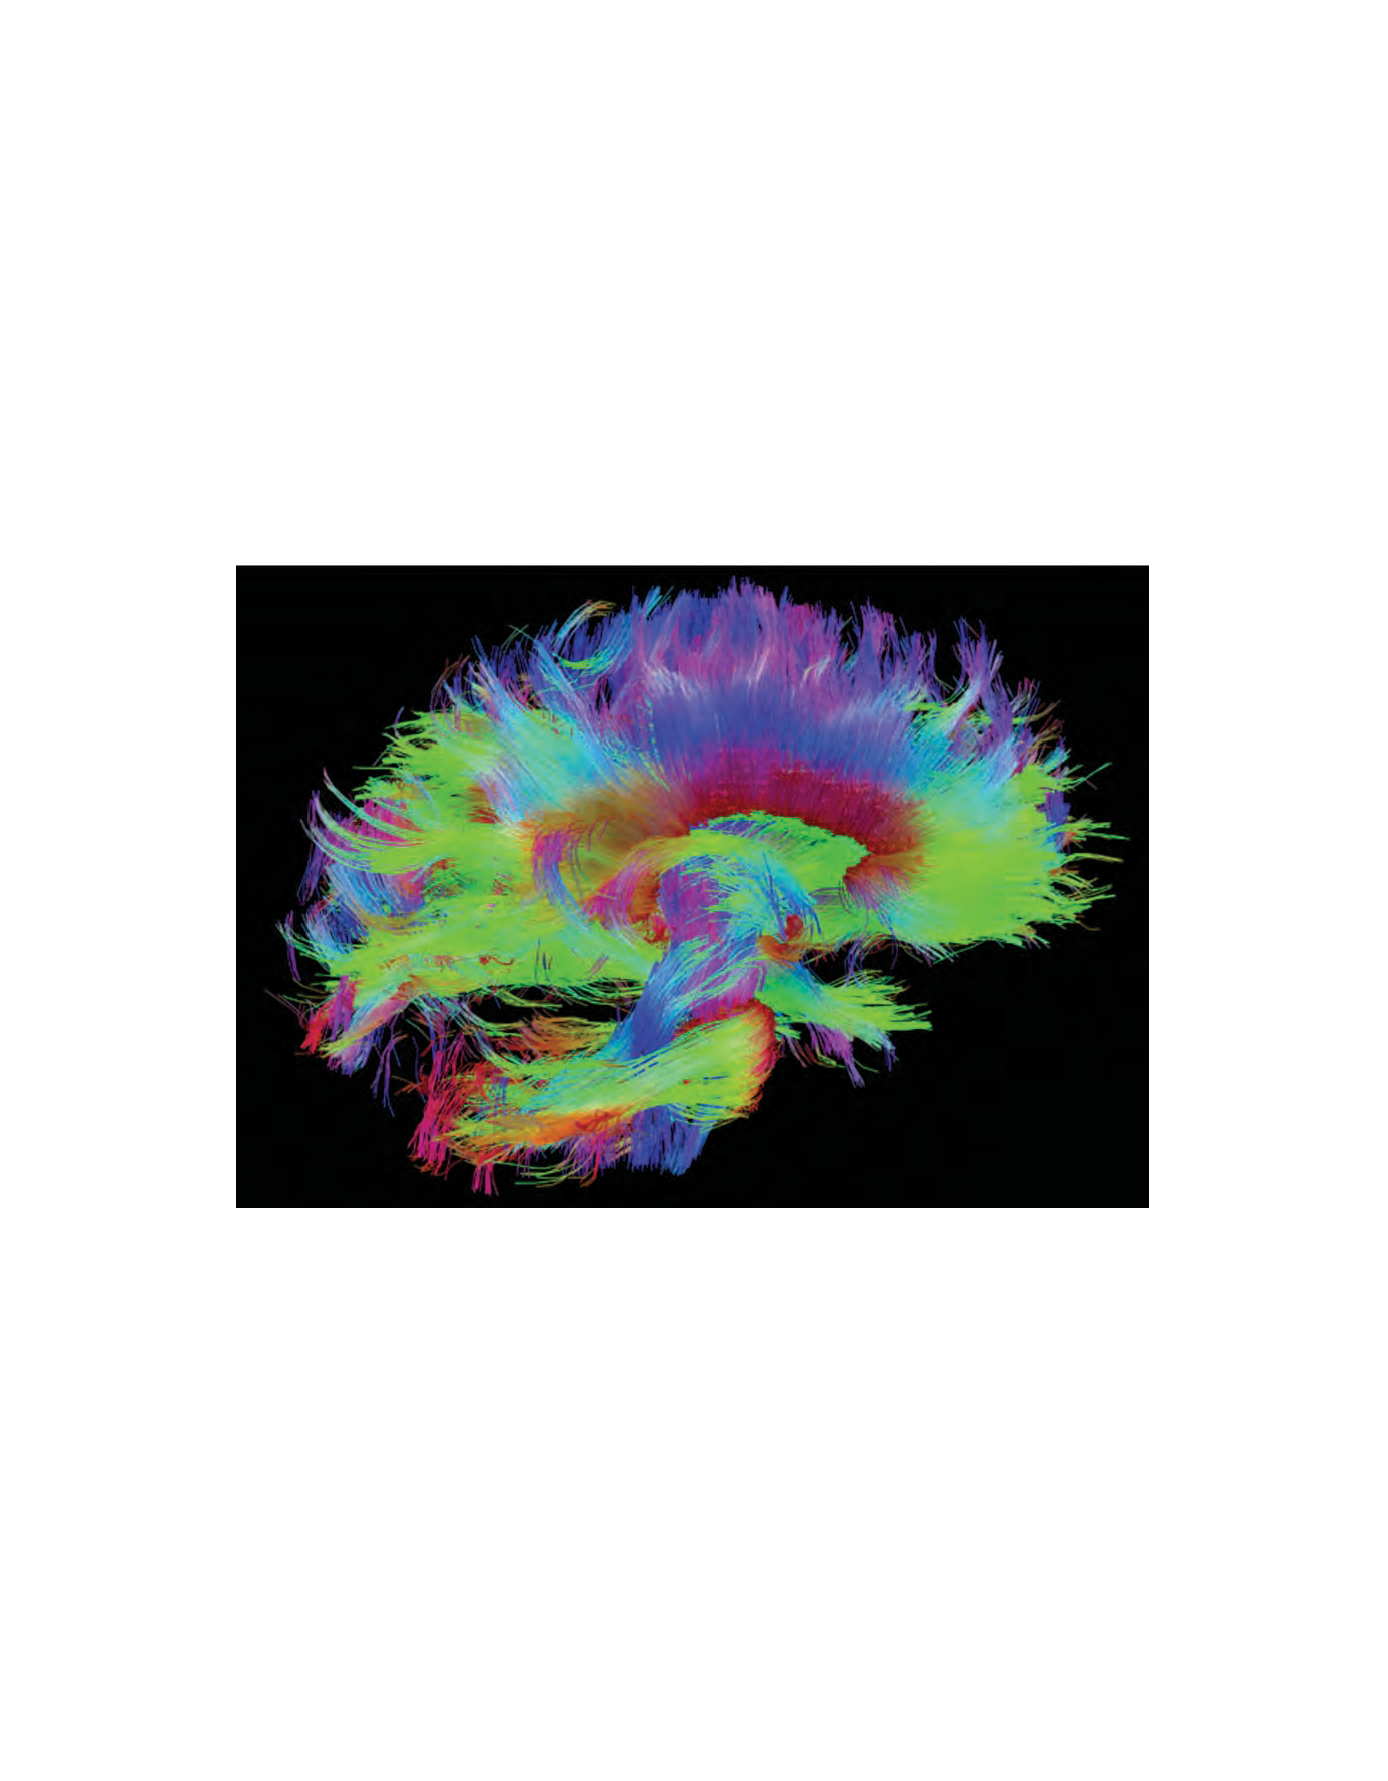
\includegraphics[width=1.0\linewidth]{chap01/fig_1_0}
	\caption{人脑白质纤维结构,显示胼胝体和脑干通路。
		该图像是根据\textit{核磁共振成像}数据和扩散光谱成像技术构建的,该技术使用水分子的扩散速率和优选方向在核磁共振图像中产生对比度,以揭示在纤维束中行进的轴突束。
		纤维按方向进行颜色编码:红色,左右;绿色,前后;蓝色,升序-降序(RGB=XYZ轴)。
		(来自连接体扫描仪数据集。
		由南加州大学神经成像实验室和哈佛大学生物医学成像中心提供。
		\href{www.humanconnetomproject.org}{人类连接体项目联合会})}
	\label{fig:1_0}
\end{figure}

在20世纪下半叶,生物学的中心焦点是基因。
现在,在21世纪上半叶,焦点已经转移到神经科学,特别是心理生物学。
我们希望了解我们感知、行动、学习和记忆的过程。
一个只有1.5公斤重的大脑器官是如何构思无限、发现新知识并产生人类思想、情感和行动的非凡个性的?
这些非凡的心理能力是如何在器官内分布的?
什么规则将一个区域的解剖组织和细胞生理与其在心理状态中的特定作用联系起来?
基因对行为有什么影响?
神经细胞中的基因表达是如何受到发育和学习过程的调节的?
经验是如何改变大脑处理后续事件的方式的,这种无意识的处理在多大程度上?
最后,神经和精神疾病的神经基础是什么?
在神经科学原理的介绍部分,我们开始讨论这些问题。
在这样做的过程中,我们描述了神经科学如何试图将神经回路的计算逻辑与大脑联系起来——定义的神经回路中的神经细胞活动如何介导复杂的心理过程。


在过去的几十年里,技术进步为大脑的科学研究开辟了新的视野。
今天,有可能将神经元互连回路的细胞动力学与大脑中感知和运动行为的内部表征联系起来,并将这些内部机制与可观察的行为联系起来。
新的成像技术使我们能够可视化人类大脑的活动——识别大脑中与特定思维和感觉模式及其相互联系模式相关的特定区域。


在本书的第一部分中,我们考虑了心理功能在多大程度上可以局限于大脑的特定区域。
我们还研究了从单个神经细胞的特性、其分子成分和突触连接的角度来理解这些功能的程度。
在本书的后面部分,我们详细研究了大脑认知和情感功能的基本机制:感知、行动、动机、情绪、学习和记忆。


人脑是一个由 800 多亿个神经细胞组成的网络,这些神经细胞在系统中相互连接——神经回路——构建我们对外部世界的感知,固定我们的注意力,指导我们的决策,并实施我们的行动。
因此,理解大脑的第一步是了解神经元是如何组织成信号通路的,以及它们是如何通过突触传递进行交流的。
我们将在本书中提出的主要观点之一是,在\textit{发育过程中建立}并在\textit{经验过程中完善}的\textit{突触连接特异性}是行为的基础。
我们还必须了解行为的先天和环境决定因素,在这些决定因素中,基因编码的蛋白质最初控制着神经回路的发育,然后可以通过基因表达的经验依赖性变化来改变神经回路。


通过将现代细胞和分子生物学技术、大脑成像、理论和临床观察应用于认知、情绪和行为的研究,一门新的心理科学正在兴起。
神经科学强化了希波克拉底在两千多年前首次提出的观点,即对心智的正确研究始于对大脑的研究。
认知心理学和精神分析理论强调了人类心理体验的多样性和复杂性。
这些学科现在可以通过从神经科学中深入了解大脑功能来丰富。
未来的任务是对心理过程进行研究,以实证神经科学为基础,关注心理的内部表征和状态是如何产生的问题。


我们的目标不仅仅是提供事实,而是提供大脑组织、功能和计算的原理。
神经科学原理并没有将人类思想的复杂性简化为一组分子或数学公理。
相反,它们让我们能够在大脑的复杂性中欣赏到某种美——达尔文式的优雅,这种复杂性解释了思维和行为。
人们可能会问,从更基本的神经机制的详细解剖中收集到的一个想法是否包含了对更高大脑功能的见解。
简单反射的组织是否与手的意志运动有关?
在发育中的脊髓中建立回路的机制是否与存储记忆的机制有关?
将我们从睡眠中唤醒的神经过程与允许无意识过程刺穿我们意识的过程相似吗?
我们希望读者在深入研究其事实基础时,会对这些原则感到高兴。
毫无疑问,这是一项正在进行的工作。





\chapter{大脑和行为} \label{chap:chap1}
生物科学的最后前沿——终极挑战——是理解意识的生物学基础和我们感知、行为、学习和记忆的大脑过程。 
在过去的几十年里,生物科学内部的显著统一为应对这一巨大挑战奠定了基础。 
对基因进行测序并推断它们编码蛋白质的氨基酸序列揭示了神经系统中的蛋白质与身体其他部位遇到的蛋白质之间意想不到的相似性。 
因此,建立细胞功能的总体计划成为可能,该计划为包括细胞神经科学在内的所有细胞生物学提供了一个共同的概念框架。


当前生物学统一的挑战是心理学——心智科学——和神经科学——大脑科学的统一。 
在这种统一的方法中,不将思想和身体视为独立的实体,基于这样一种观点,即所有行为都是大脑功能的结果。 
我们通常所说的心智,就是大脑进行的一系列操作。 
大脑过程不仅是行走和进食等简单运动行为的基础,也是典型人类的所有复杂认知和行为的基础——思考、说话和创作艺术作品。 
作为推论,所有表征精神疾病的行为障碍——情感障碍(感觉)和认知障碍(思想)——都是脑功能紊乱的结果。


大脑中数十亿个神经细胞如何产生行为和认知状态,以及这些细胞如何受到环境(包括社会经验)的影响? 
用大脑活动来解释行为是神经科学的重要任务,神经科学在这方面的进展是本书的一大主题。


神经科学必须不断面对某些基本问题。 
理解思维过程、肢体运动或做出运动愿望的适当生物学描述水平是多少? 
为什么在某些神经系统疾病状态下运动会平稳或急促或无意中进行? 
通过观察神经细胞中\textit{脱氧核糖核酸}表达的模式以及这种模式如何调节神经元的电特性,可能会得出这些问题的答案。 
然而,我们还需要了解由特定大脑区域中的许多神经元组成的神经回路以及许多大脑区域中特定回路的活动如何协调的知识。


是否存在最恰当的生物学描述水平?
简短的回答是,
如果一个人的目标是了解和治疗某些遗传性癫痫病症,那么\textit{脱氧核糖核酸}测序和单个神经元电特性的测量可能足以产生有效的治疗方法。
如果一个人对学习、感知和探索感兴趣,那么可能需要对回路系统和大脑区域进行分析。


现代神经科学的目标是将所有这些专业水平整合成一门连贯的科学。
这种努力迫使我们面对新的问题。
如果心理过程可以定位到离散的大脑区域,那么这些区域的功能与这些区域的解剖学和生理学之间的关系是什么? 
是否需要一种神经回路来处理视觉信息,另一种神经回路来解析语音,还有另一种神经回路来排列运动?
或者具有不同功能的回路是否具有共同的组织原则?
必要的神经计算是否最好理解为对单个神经元或神经元群表示的信息的操作?
信息是以单个神经细胞的电活动表示的,还是分布在整体上的,以至于任何一个细胞的信息量都不比计算机内存的随机位多?
正如我们将要看到的,关于组织水平、细胞特化和功能定位的问题在整个神经科学中反复出现。


为了说明这些观点,我们将研究现代神经科学如何描述语言,这是人类独特的认知行为。
这样做将广泛关注大脑皮层的运作,大脑皮层是人类大脑中最发达的部分。
将看到大脑皮层如何组织成功能不同的区域,每个区域由许多神经元组成,以及如何根据特定区域内特定组互连神经元的活动来分析高度复杂行为的神经装置。
第~\ref{chap:chap3}~章描述了简单反射行为的神经回路如何在细胞水平上运作,说明了感觉信号和运动信号的相互作用如何导致运动行为。



% 结构(几何)和功能(行为)
\section{关于大脑与行为之间的关系,提出了两种相反的观点}

关于神经细胞、大脑和行为的观点是在 20 世纪从 5 种实验传统的综合中产生的:解剖学、胚胎学、生理学、药理学和心理学。


公元 2 世纪的希腊医生盖伦提出,神经将大脑和脊髓分泌的液体输送到身体的周围。
他的观点主导了西方医学,直到显微镜揭示了神经组织中细胞的真实结构。
即便如此,直到 19 世纪后期,神经组织才成为一门特殊科学的主题,当时意大利人\textit{卡米洛$\cdot$高尔基}和西班牙人圣地\textit{亚哥$\cdot$拉蒙$\cdot$卡哈尔}对神经细胞进行了详细、准确的描述,但就大脑的功能得出了两个截然不同的结论。


高尔基开发了一种用银盐对神经元进行染色的方法,这种方法可以在显微镜下显示出它们的整个细胞结构。
基于这些研究,高尔基体得出结论,神经细胞不是相互隔离的独立细胞,而是在一个连续的组织或合胞体网络中共同作用。
使用高尔基技术,\textit{卡哈尔}扩观察到每个神经元通常都有一个细胞体和两种类型的过程:一端是分支树突,另一端是长长的电缆状轴突。 
\textit{卡哈尔}扩得出结论,神经组织不是合胞体,而是离散细胞网络。
在这项工作的过程中,\textit{卡哈尔}扩发展了神经元学说的一些关键概念和许多早期证据——个体神经元是神经系统的基本构建块和信号元件的原则。


在 1920 年,美国胚胎学家\textit{罗斯$\cdot$哈里逊}表明树突和轴突是从细胞体中生长出来的,即使在组织培养中每个神经元都与其他神经元隔离开来也是如此。
\textit{哈里逊}还证实了\textit{卡哈尔}的提议,即轴突的尖端会产生扩张,即生长锥,它将发育中的轴突引导至其目标,即其他神经细胞或肌肉。
这两项发现都为神经元学说提供了强有力的支持。
随着电子显微镜的引入,神经元学说的最终明确证据出现在 20 世纪 50 年代中期。
\textit{桑福德$\cdot$帕莱}的一项具有里程碑意义的研究明确地证明了突触的存在,突触是神经细胞的特殊区域,允许它们之间进行化学或电信号传递。


神经系统的生理学研究始于 18 世纪后期,当时意大利医师和物理学\textit{路易吉$\cdot$加尔瓦尼}发现肌肉和神经细胞会产生电能。
现代电生理学起源于 19 世纪三位德国生理学家——\textit{约翰内斯$\cdot$米勒}、\textit{埃米尔$\cdot$杜$\cdot$博伊斯-雷蒙德}和\textit{赫尔曼$\cdot$冯$\cdot$亥姆霍兹}——他们成功地测量了电活动沿神经细胞轴突的传导速度,并进一步表明:
一个神经细胞的电活动以可预测的方式影响相邻细胞的活动。


药理学在 19 世纪末对我们对神经系统和行为的理解产生了第一次影响,当时法国的\textit{克劳德$\cdot$伯纳德}、德国的\textit{保罗$\cdot$埃尔利希}和英国的\textit{约翰$\cdot$兰利}证明药物不会随机作用于细胞,而是通常与位于细胞膜中的离散受体结合。 
这种洞察力导致发现神经细胞可以通过化学方式相互交流。


关于行为的心理学思考可以追溯到西方科学的开端,当时古希腊哲学家推测行为的原因以及心灵与大脑的关系。
在随后的几个世纪里,出现了两种主要观点。
在 17 世纪,笛卡尔区分了身体和心灵。
在这种二元论观点中,大脑调解了知觉、运动行为、记忆、食欲和激情——一切可以在低等动物身上找到的东西。
但是心智——更高的心智功能,人类行为的有意识体验特征——并不代表大脑或身体的任何其他部分,而是代表灵魂,一个精神实体。
笛卡尔认为,灵魂通过松果体与大脑的机器进行交流,松果体是大脑中线的一个微小结构。
笛卡尔的立场在现代哲学或神经科学中几乎没有影响力。 
事实上,神经科学的基本前提是心智是大脑及其神经活动的产物。
我们这样说并不是说神经科学的目的是通过还原为生物成分来解释心灵,而是要阐明心灵的生物学。


早在 1800 年,维也纳医生和神经解剖学家\textit{弗朗兹$\cdot$约瑟夫$\cdot$加尔}就开始尝试将生物学和心理学概念结合到行为研究中,当时他提出了一种全新的身心观念。
他主张大脑是心灵的器官,一切精神功能都体现在大脑中。
因此,他拒绝了笛卡尔认为思想和身体是分开实体的观点。
此外,他认为大脑皮层不是一个单一的器官,而是包含许多专门的器官,大脑皮层的特定区域控制着特定的功能。 
\textit{加尔}列举了至少 27 个不同的大脑皮层区域或器官; 后来又增加了更多,每一种都对应于一种特定的心智能力(图~\ref{fig:1_1})。
\textit{加尔}将智力过程(例如评估因果关系、计算和感知秩序的能力)分配给了大脑的前部。
浪漫的爱情(恋爱)和好斗的本能特征被分配到大脑后部。
即使是最抽象的人类行为——慷慨、隐秘和虔诚——也被分配到大脑中的一个位置。


\begin{figure}[htbp]
	\centering
	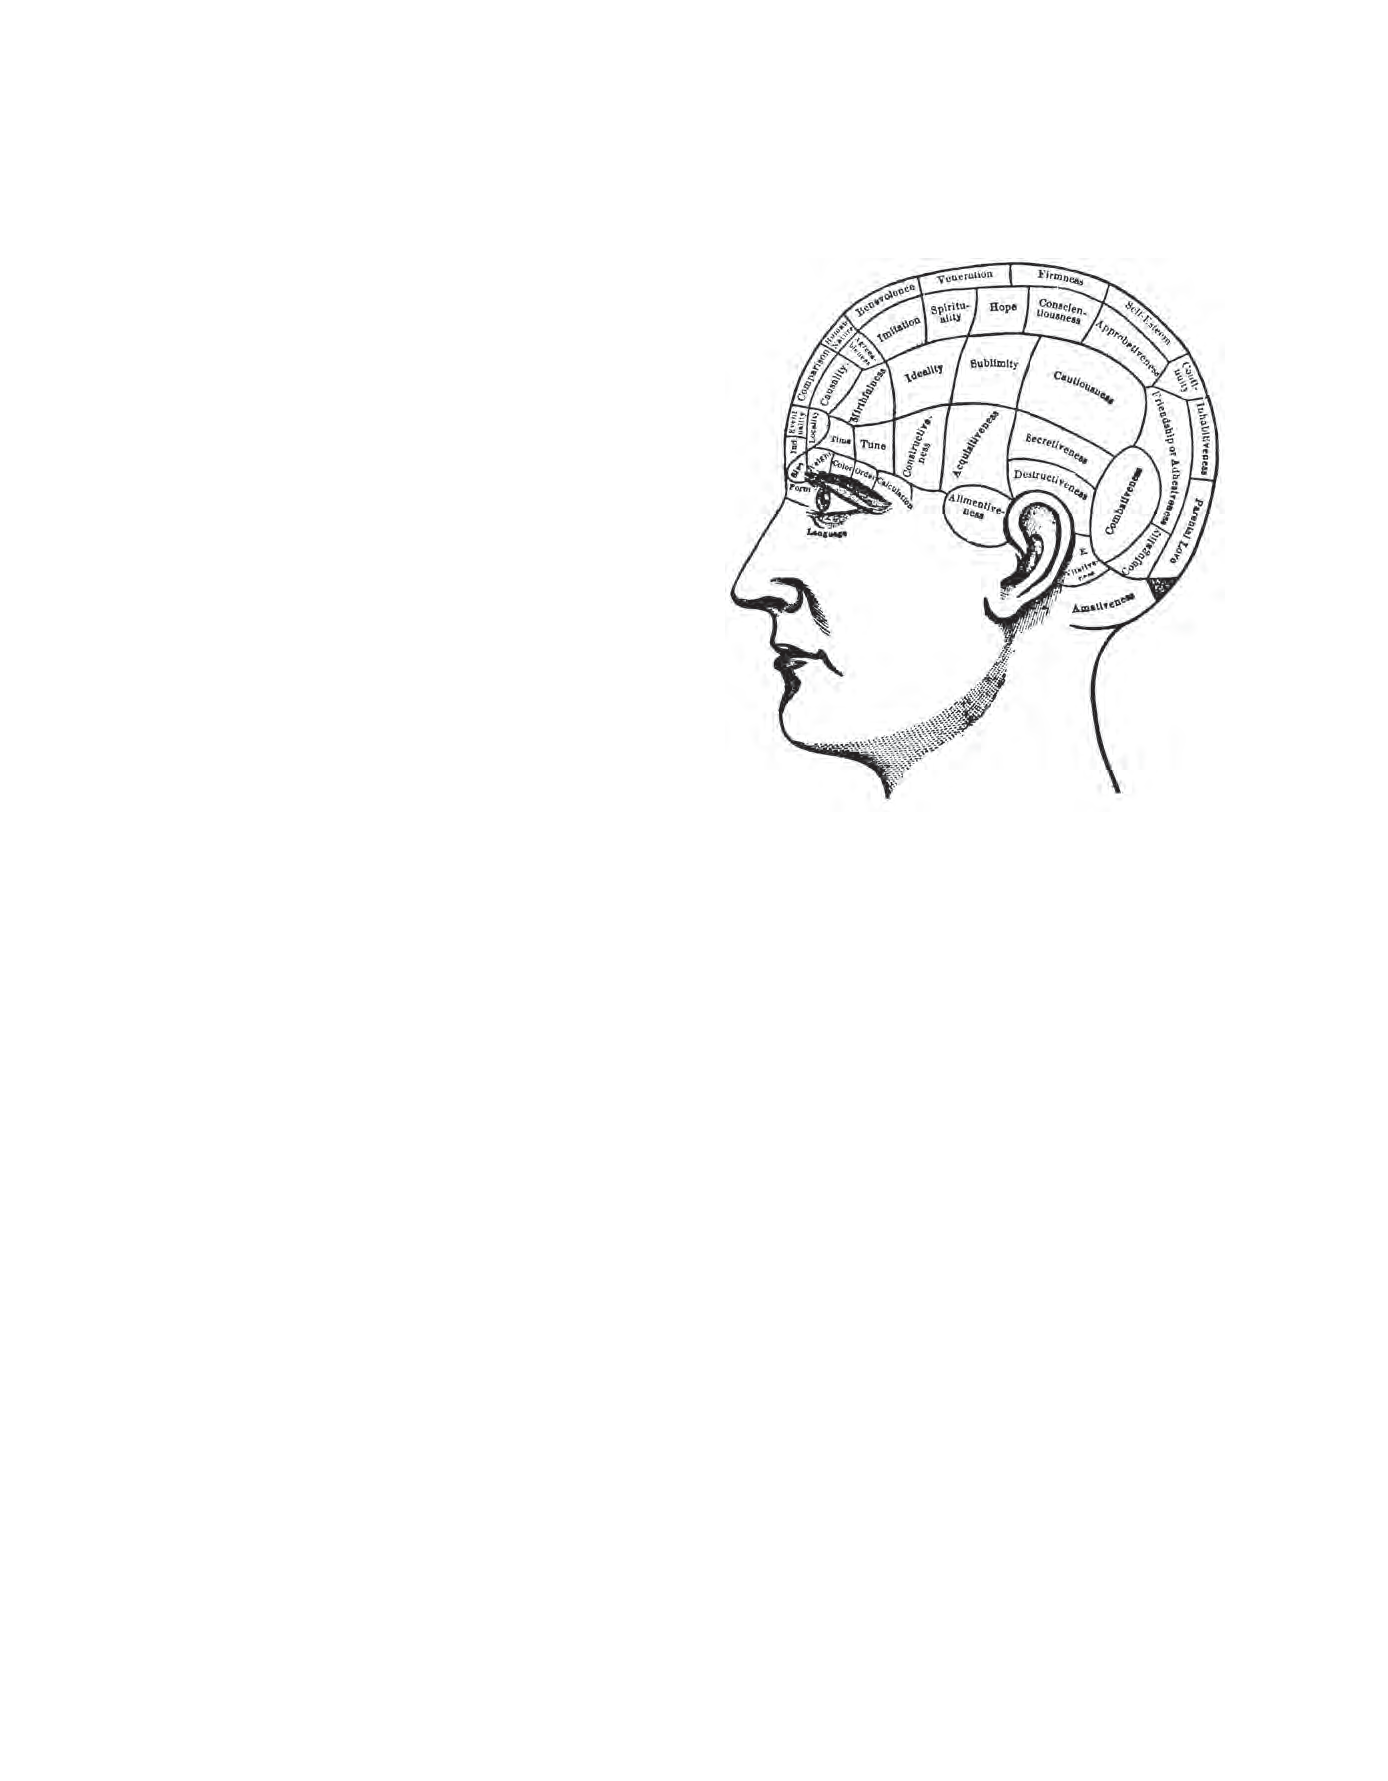
\includegraphics[width=0.55\linewidth]{chap01/fig_1_1}
	\caption{大脑功能定位的早期地图。
		根据 19 世纪的颅相学学说,好斗、灵性、希望和责任心等复杂特征由专门的“器官”控制,大脑皮层的不同区域随着特征的发展而扩大。
		这些大脑局部区域的扩大被认为会在覆盖的头骨上产生特征性的凹凸,从中可以确定一个人的性格。
		这张地图取自 1800 年代初期的一幅图画,显示了 42 个智力和情感“器官”。}
	\label{fig:1_1}
\end{figure}


尽管\textit{加尔}的身心统一理论和他关于某些功能局限于特定大脑区域的观点被证明是正确的,但今天的主流观点是,许多高级心理功能很可能是高度分布的。
此外,\textit{加尔}的本地化实验方法极其幼稚。
\textit{加尔}没有根据经验定位功能,而是通过研究大脑并将心理属性的缺陷与肿瘤或中风后特定区域的病变相关联,\textit{加尔}摒弃了所有来自脑部病变研究的证据,无论是通过临床检查发现的还是在实验动物身上通过手术产生的。
受\textit{相面术}的影响,这是一门基于面部特征揭示性格的流行科学,\textit{加尔}认为,具有特定认知能力的人头骨上的隆起和隆起确定了大脑中这些能力的中心。
他假设大脑区域的大小与该区域所代表的心智能力的相对重要性有关。
因此,特定智力的锻炼会导致相应的大脑区域生长,而这种生长又会导致覆盖在上面的头骨突出。


小时候,\textit{加尔}注意到他那些擅长背作业的同学都有突出的眼睛,于是他就有了这个想法。
他得出结论,这是大脑前部与语言记忆有关的区域过度发育的结果。
当他还是一名年轻医生时,他进一步发展了这个想法,负责管理维也纳的一家精神病院。
在那里,他开始研究患有偏执狂症的患者,这种疾病的特征是对某些关键思想过分感兴趣或强烈渴望从事某些特定行为——盗窃、谋杀、色情、极端宗教信仰。
他推断,由于患者在所有其他行为中都表现良好,大脑缺陷一定是离散的,原则上可以通过检查这些患者的头骨来定位。
\textit{加尔}对局部大脑功能的研究催生了颅相学,这是一门根据头骨的详细形状确定人格和性格的学科。


在 1820 年代后期,法国生理学家\textit{皮埃尔$\cdot$弗卢龙}对\textit{加尔}的想法进行了实验分析。 
\textit{弗卢龙}使用实验动物破坏了\textit{加尔}在大脑中的一些功能中心,进而试图分离出这些“大脑器官”对行为的贡献。
从这些实验中,\textit{弗卢龙}得出结论,特定的大脑区域并不负责特定的行为,而是所有的大脑区域,尤其是前脑的大脑半球,都参与了每一次心理操作。
\textit{弗卢龙}提出,大脑半球的任何部分都有助于半球的所有功能。
因此,大脑半球任何一个区域的损伤都应该平等地影响所有更高的功能。
因此,在 1823 年,\textit{弗卢龙}写道:“所有知觉、所有意志都在这些(大脑)器官中占据相同的位置;
因此,知觉、构想和意志的能力仅仅构成了一种本质上是一体的能力。”


这种信念的迅速接受,后来被称为大脑的整体观点,仅部分基于\textit{弗卢龙}的实验工作。
它也代表了对人类思想是生物器官的唯物主义观点的文化反应。
它代表了对没有灵魂、所有心理过程都可以简化为大脑内的活动以及可以通过锻炼来改善思想的观念的拒绝——这些想法是欧洲宗教机构和土地贵族所不能接受的。


然而,在 19 世纪中叶,法国神经学家\textit{皮埃尔$\cdot$保尔$\cdot$布罗卡}、德国神经学家\textit{卡尔$\cdot$韦尼克}和英国神经学家\textit{休林斯$\cdot$杰克逊}严重挑战了整体观点。
例如,杰克逊在他对局灶性癫痫(一种以身体特定部位开始抽搐为特征的疾病)的研究中表明,不同的运动和感觉功能可以追溯到大脑皮层的特定部位。
\textit{布洛卡}、\textit{韦尼克} 和\textit{杰克逊}的区域研究被 \textit{查尔斯$\cdot$谢灵顿}和\textit{卡哈尔}扩展到细胞水平,他们支持称为细胞连接主义的大脑功能观点。
根据这种观点,单个神经元是大脑的信号单元;
它们按功能组排列,并以精确的方式相互连接。
\textit{韦尼克}和法国神经学家\textit{朱尔斯$\cdot$代热林}的研究表明,不同的行为是由不同的相互关联的大脑区域产生的。


本地化的第一个重要证据来自对大脑如何产生语言的研究。
在考虑相关的临床和解剖学研究之前,首先要回顾一下大脑的整体结构,包括它的主要解剖区域。
这需要我们定义一些神经解剖学家用来描述大脑和脊髓部分之间三维空间关系的基本导航术语。
这些术语在框~\ref{box:1_1}~和图~\ref{fig:1_2}~中介绍。


\begin{proposition}[神经解剖学导航术语] \label{box:1_1}
	
	\quad \quad 中枢神经系统各组成部分在体内的位置和方向参照三个轴进行描述:嘴侧-尾侧、背侧-腹侧和内侧-外侧轴(图~\ref{fig:1_2})。
	这些术语使神经解剖学家能够描述大脑和脊髓部分之间的空间关系。
	它们有助于在同一物种的个体发育或疾病情况下对其大脑进行比较。
	例如,它们也有助于比较不同动物物种的大脑,以了解大脑的进化。

\end{proposition}


\begin{figure}[htbp]
	\centering
	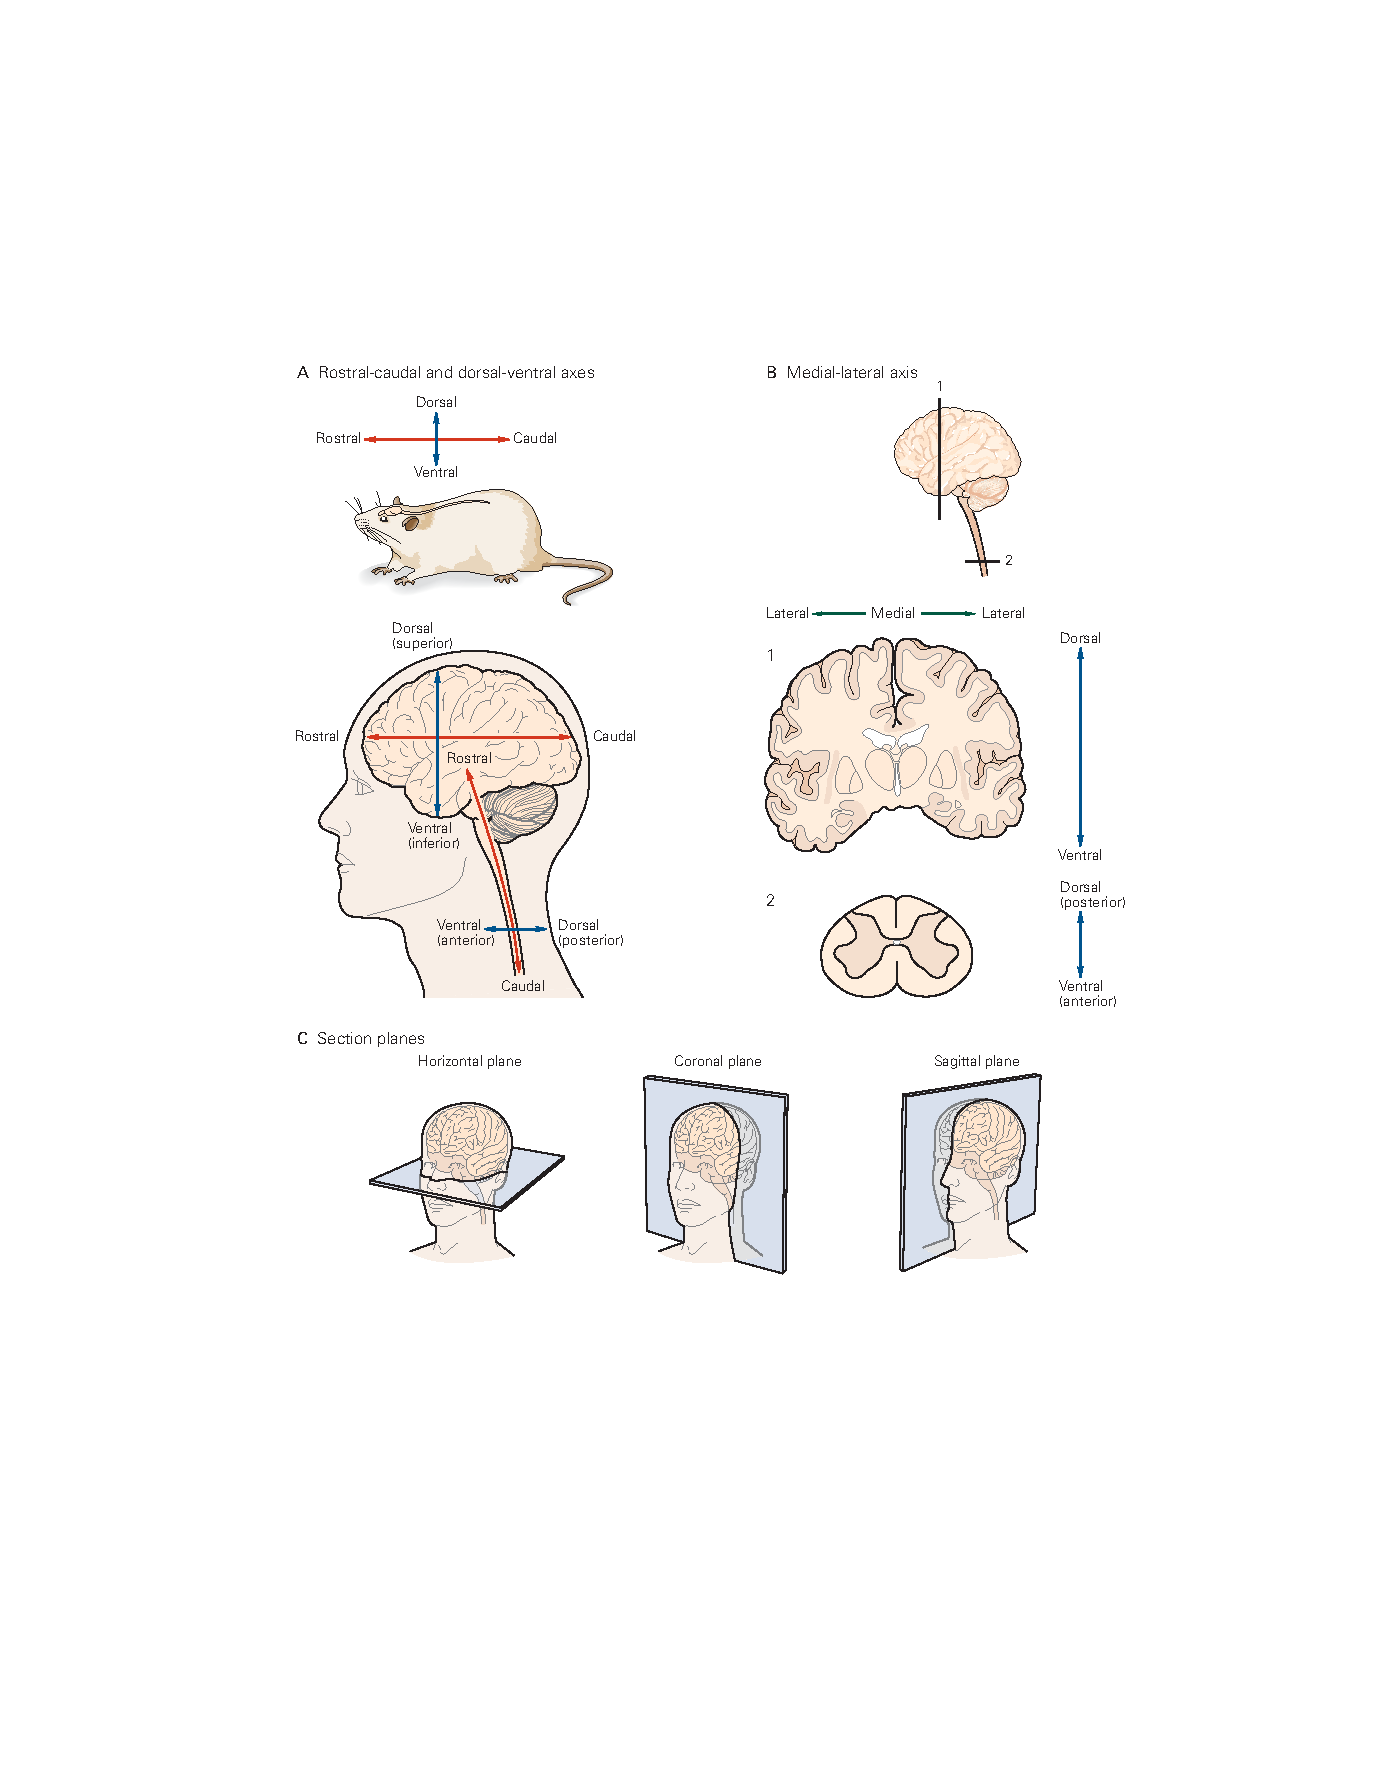
\includegraphics[width=0.9\linewidth]{chap01/fig_1_2}
	\caption{中枢神经系统沿着三个主要轴进行描述\cite{martin2012neuroanatomy}。 
		\textbf{A.} 嘴侧表示朝向鼻子和尾部朝向尾巴。
		背侧是指朝向动物的背部,腹侧是指朝向腹部。
		在低等哺乳动物中,这两个轴的方向在发育到成年生活的过程中一直保持不变。
		在人类和其他高等灵长类动物中,纵轴在脑干中弯曲大约 110 度。
		由于这种挠曲,相同的位置术语在指代挠曲下方和上方的结构时具有不同的含义。
		在弯曲下方,在脊髓中,嘴侧意味着朝向头部,尾侧意味着朝向尾骨(脊柱的下端),腹侧(前侧)意味着朝向腹部,背侧(后侧)意味着朝向背部。
		在弯曲上方,嘴侧意味着朝向鼻子,尾侧意味着朝向后脑勺,腹侧意味着朝向下巴,背侧意味着朝向头顶。
		术语上位通常与背侧同义,下位与腹侧相同。
		\textbf{B.} 内侧意味着朝向大脑中部,外侧意味着朝向侧面。
		\textbf{C.} 当对大脑进行切片进行分析时,切片通常是在三个基本平面之一中制作的:水平、冠状或矢状。}
	\label{fig:1_2}
\end{figure}



\section{大脑具有不同的功能区域}

中枢神经系统是一个双侧且基本对称的结构,有两个主要部分,即脊髓和大脑。
大脑包括六个主要结构:延髓、脑桥、小脑、中脑、间脑和大脑(方框~\ref{box:1_2}~和图~\ref{fig:1_3})。
这些中的每一个依次包含具有独特连接性和发育起源的不同神经元组。
在延髓、脑桥、中脑和间脑中,神经元通常分为不同的簇,称为细胞核。
大脑和小脑的表面由一大片折叠的神经元组成,分别称为大脑皮层和小脑皮层,其中神经元以固定的连接模式分层组织。
大脑还包含许多位于皮层(皮层下)下方的结构,包括基底神经节和杏仁核(图~\ref{fig:1_4})。


\begin{proposition}[中枢神经系统的解剖学组织] \label{box:1_2}
	\textbf{中枢神经系统有七个主要部分}
	
	\quad \quad \textbf{脊髓}是中枢神经系统的最尾部,接收和处理来自四肢和躯干皮肤、关节和肌肉的感觉信息,并控制四肢和躯干的运动。
	如图~\ref{fig:1_3}~所示,它被细分为颈部、胸部、腰部和骶骨区域。
	
	\quad \quad 脊髓继续作为\textbf{脑干}向头端延伸,脑干由延髓、脑桥和中脑组成。
	脑干接收来自头部皮肤和肌肉的感觉信息,并为头部肌肉组织提供运动控制。
	它还将信息从脊髓传递到大脑,从大脑传递到脊髓,并通过网状结构调节唤醒和意识水平。
	
	\quad \quad 脑干包含几个细胞体集合,即脑神经核。
	其中一些细胞核接收来自头部皮肤和肌肉的信息;
	其他人控制面部、颈部和眼睛肌肉的运动输出。
	还有一些人专门处理来自三种特殊感官的信息:听觉、平衡和味觉。
	
	\quad \quad \textbf{延髓}直接位于脊髓的嘴侧,包括几个负责重要自主功能的中心,如消化、呼吸和心率控制。
	
	\quad \quad \textit{脑桥},从嘴侧到髓质,传递从大脑半球到小脑的运动信息。
	
	\quad \quad 脑桥后面的\textbf{小脑}调节运动的力量和范围,并参与运动技能的学习。
	它在功能上与脑干的三个主要器官相连:延髓、脑桥和中脑。
	
	\quad \quad \textbf{中脑}位于脑桥的嘴侧,控制着许多感觉和运动功能,包括眼球运动以及视觉和听觉反射的协调。
	
	\quad \quad \textbf{间脑}位于中脑的嘴侧,包含两个结构。
	丘脑处理从中枢神经系统其他部分到达大脑皮层的大部分信息。
	下丘脑调节自主神经、内分泌和内脏功能。
	
	\quad \quad \textbf{大脑}由两个大脑半球组成,每个半球由褶皱严重的外层(大脑皮层)和三个深层结构(基底神经节、海马体和杏仁核的组成部分)组成。
	基底神经节包括尾状核、壳核和苍白球,调节运动执行、运动和习惯学习,这两种记忆形式被称为内隐记忆;
	海马体对储存人、地点、事物和事件的记忆至关重要,这种记忆形式被称为外显记忆;
	杏仁核协调情绪状态的自主神经和内分泌反应,包括威胁记忆,另一种形式的内隐记忆。
	
	\quad \quad 如图~\ref{fig:1_3}~所示,每个大脑半球分为四个不同的叶:额叶、顶叶、枕叶和颞叶。
	这些叶与不同的功能有关,尽管皮层区域都高度互联,可以参与广泛的大脑功能。
	枕叶接收视觉信息,对视觉的各个方面都至关重要。
	来自枕叶的信息通过两个主要途径进行处理。
	连接枕叶和顶叶的背流与视觉空间中物体的位置和操作有关。
	连接枕叶和颞叶的腹侧流与物体身份有关,包括对单个人脸的识别。
	颞叶对处理听觉信息也很重要(它还包含隐藏在其表面下的海马体和杏仁核)。
	额叶与所有皮层区域紧密相连,对高级认知处理和运动规划很重要。
	
	\quad \quad 大约三分之二的皮层位于脑沟中,许多脑回被覆盖的皮层叶所掩埋。
	通过分离大脑半球以显示大脑的内侧表面,并在死后对大脑进行切片,例如在尸检中,可以看到大脑皮层的完整范围(图~\ref{fig:1_4})。
	这些信息中的大部分可以通过现代大脑成像在活体大脑中可视化(图~\ref{fig:1_5};第~\ref{chap:chap6}~章)。
	这些观点也提供了白质和皮层下灰质的观点。
	
	\quad \quad 大脑皮层表面看不到的两个重要区域包括扣带皮层和岛叶皮层。
	扣带皮层位于胼胝体的背面,对情绪、疼痛感知和认知的调节很重要。
	岛叶皮层位于上覆的额叶、顶叶和颞叶内,在情绪、稳态和味觉感知中发挥着重要作用。
	这些内部视图还提供了对\textit{胼胝体}的检查,\textit{胼胝}体是连接两个半球的突出轴突\textit{纤维束}。
	
	上述不同的大脑区域通常分为三个更广泛的区域:后脑(包括延髓、脑桥和小脑);
	中脑(包括顶盖、黑质、网状结构和中脑导水管周围灰质);
	和前脑(包括间脑和大脑)。
	中脑和后脑(减去小脑)包括与脑干相同的结构。
	神经系统的解剖组织在第~\ref{chap:chap4}~章中有更详细的描述。
		
\end{proposition}


\begin{figure}[htbp]
	\centering
	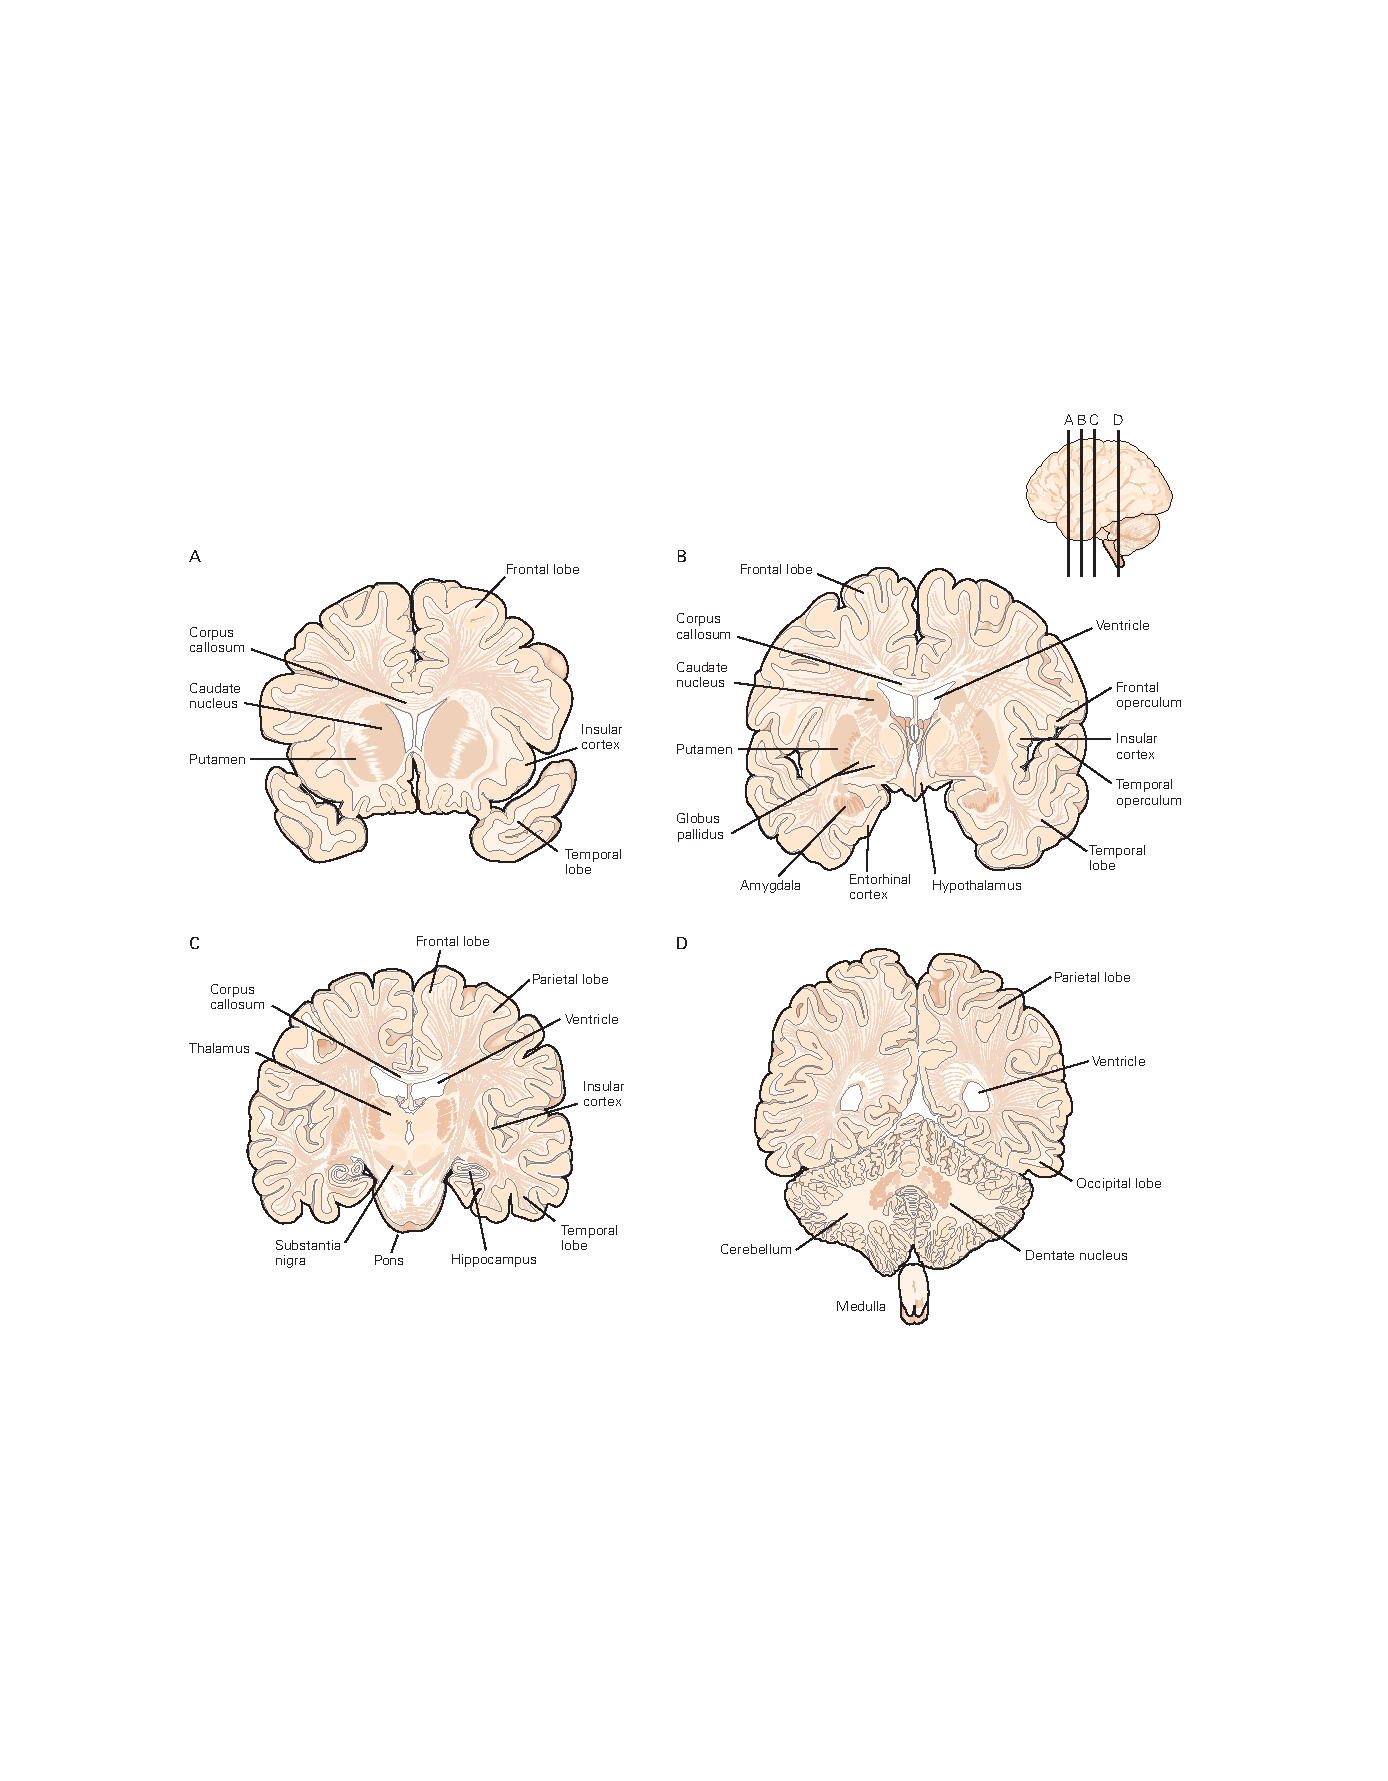
\includegraphics[width=0.95\linewidth]{chap01/fig_1_4}
	\caption{中枢神经系统的划分。
		\textbf{A.} 中枢神经系统可分为七个主要区域,从最尾部的脊髓区域,到脑干(延髓、脑桥和中脑),到间脑(包括丘脑和下丘脑),到端脑或大脑(大脑皮层、底层白质、皮层下核和基底神经节)。
		\textbf{B.} 大脑的四个主要叶以覆盖它们的颅骨部分命名。
		这张大脑的侧视图仅显示左侧大脑半球。
		中央沟将额叶和顶叶分开。
		外侧沟将额叶与颞叶分开。
		初级运动皮层占据紧靠中央沟头端的回。
		初级体感皮层占据中央沟尾部的回。
		\textbf{C.} 在右半球的内侧视图中,当半球分开时,可以看到大脑的进一步分裂。
		\textit{胼胝体}包含一大束连接两个半球的轴突。
		扣带皮层是大脑皮层的一部分,围绕着大脑皮层。
		初级视觉皮层占据距状沟。}
	\label{fig:1_3}
\end{figure}


\begin{figure}[htbp]
	\centering
	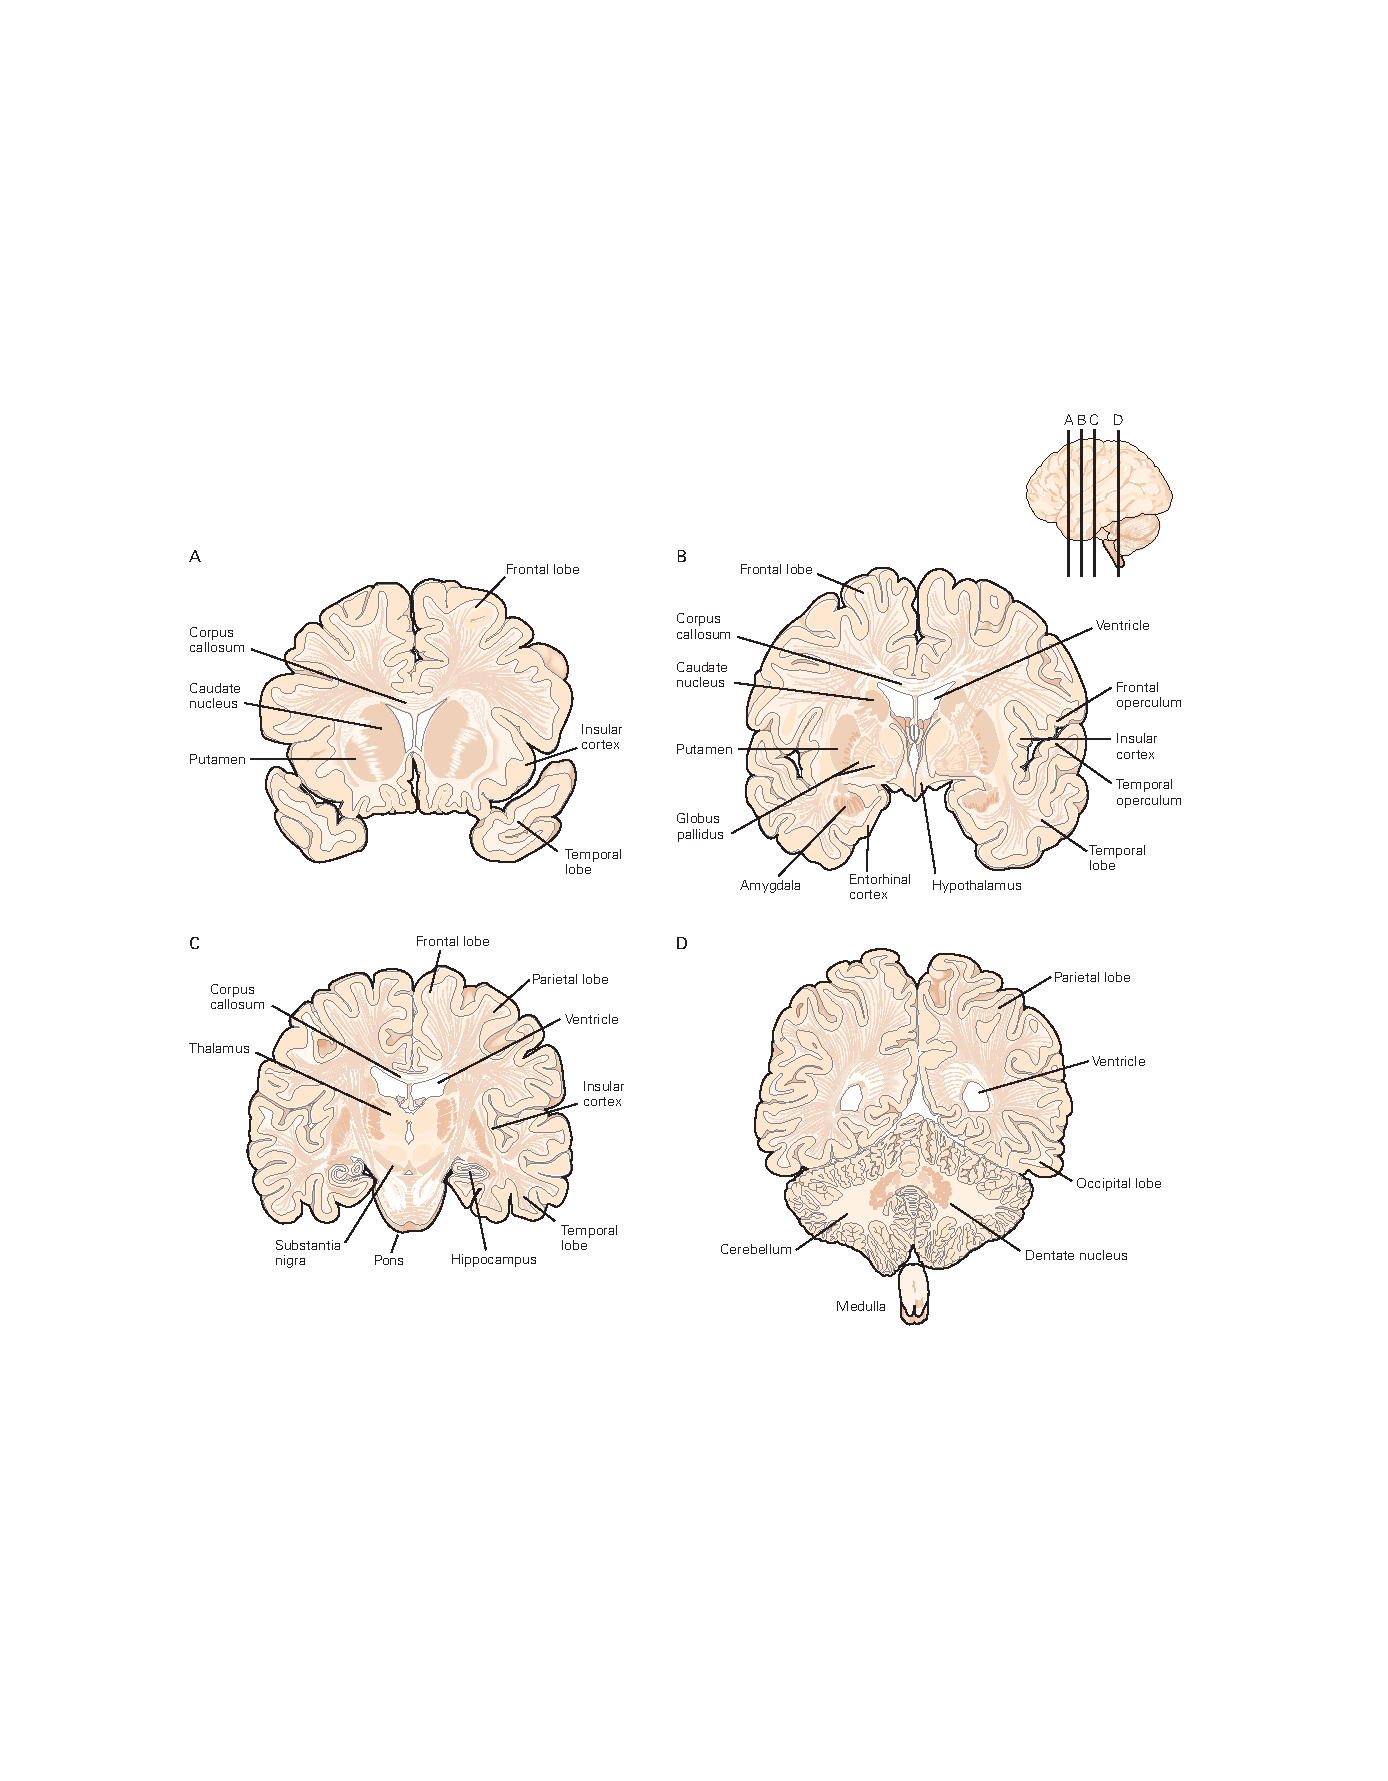
\includegraphics[width=0.8\linewidth]{chap01/fig_1_4}
	\caption{在死后组织的脑切片图中可以看到大脑半球的主要皮层下和深部皮层区域。
		四个连续的冠状切片 (A–D) 沿着大脑侧视图(右上角,插图)上指示的延髓-尾轴制作。
		基底神经节包括尾状核、壳核、苍白球、黑质和底丘脑核(未显示)。
		丘脑将感觉信息从外围传递到大脑皮层。
		杏仁核和海马体是埋藏在颞叶内的大脑皮层区域,对情绪反应和记忆很重要。
		脑室包含并产生脑脊液,脑脊液浸润脑沟、脑池和脊髓\cite{nieuwenhuys2007human}。}
	\label{fig:1_4}
\end{figure}


现代脑成像技术可以看到活人这些结构的活动(见第~\ref{chap:chap6}~章)。
当人们在受控条件下从事特定任务时,脑成像通常用于评估大脑离散区域的代谢活动。
这些研究提供的证据表明,特定类型的行为比其他行为更能激发大脑特定区域的活动。
大脑成像生动地表明认知操作主要依赖于大脑皮层,即覆盖两个大脑半球的皱纹灰质(图~\ref{fig:1_5})。


\begin{figure}[htbp]
	\centering
	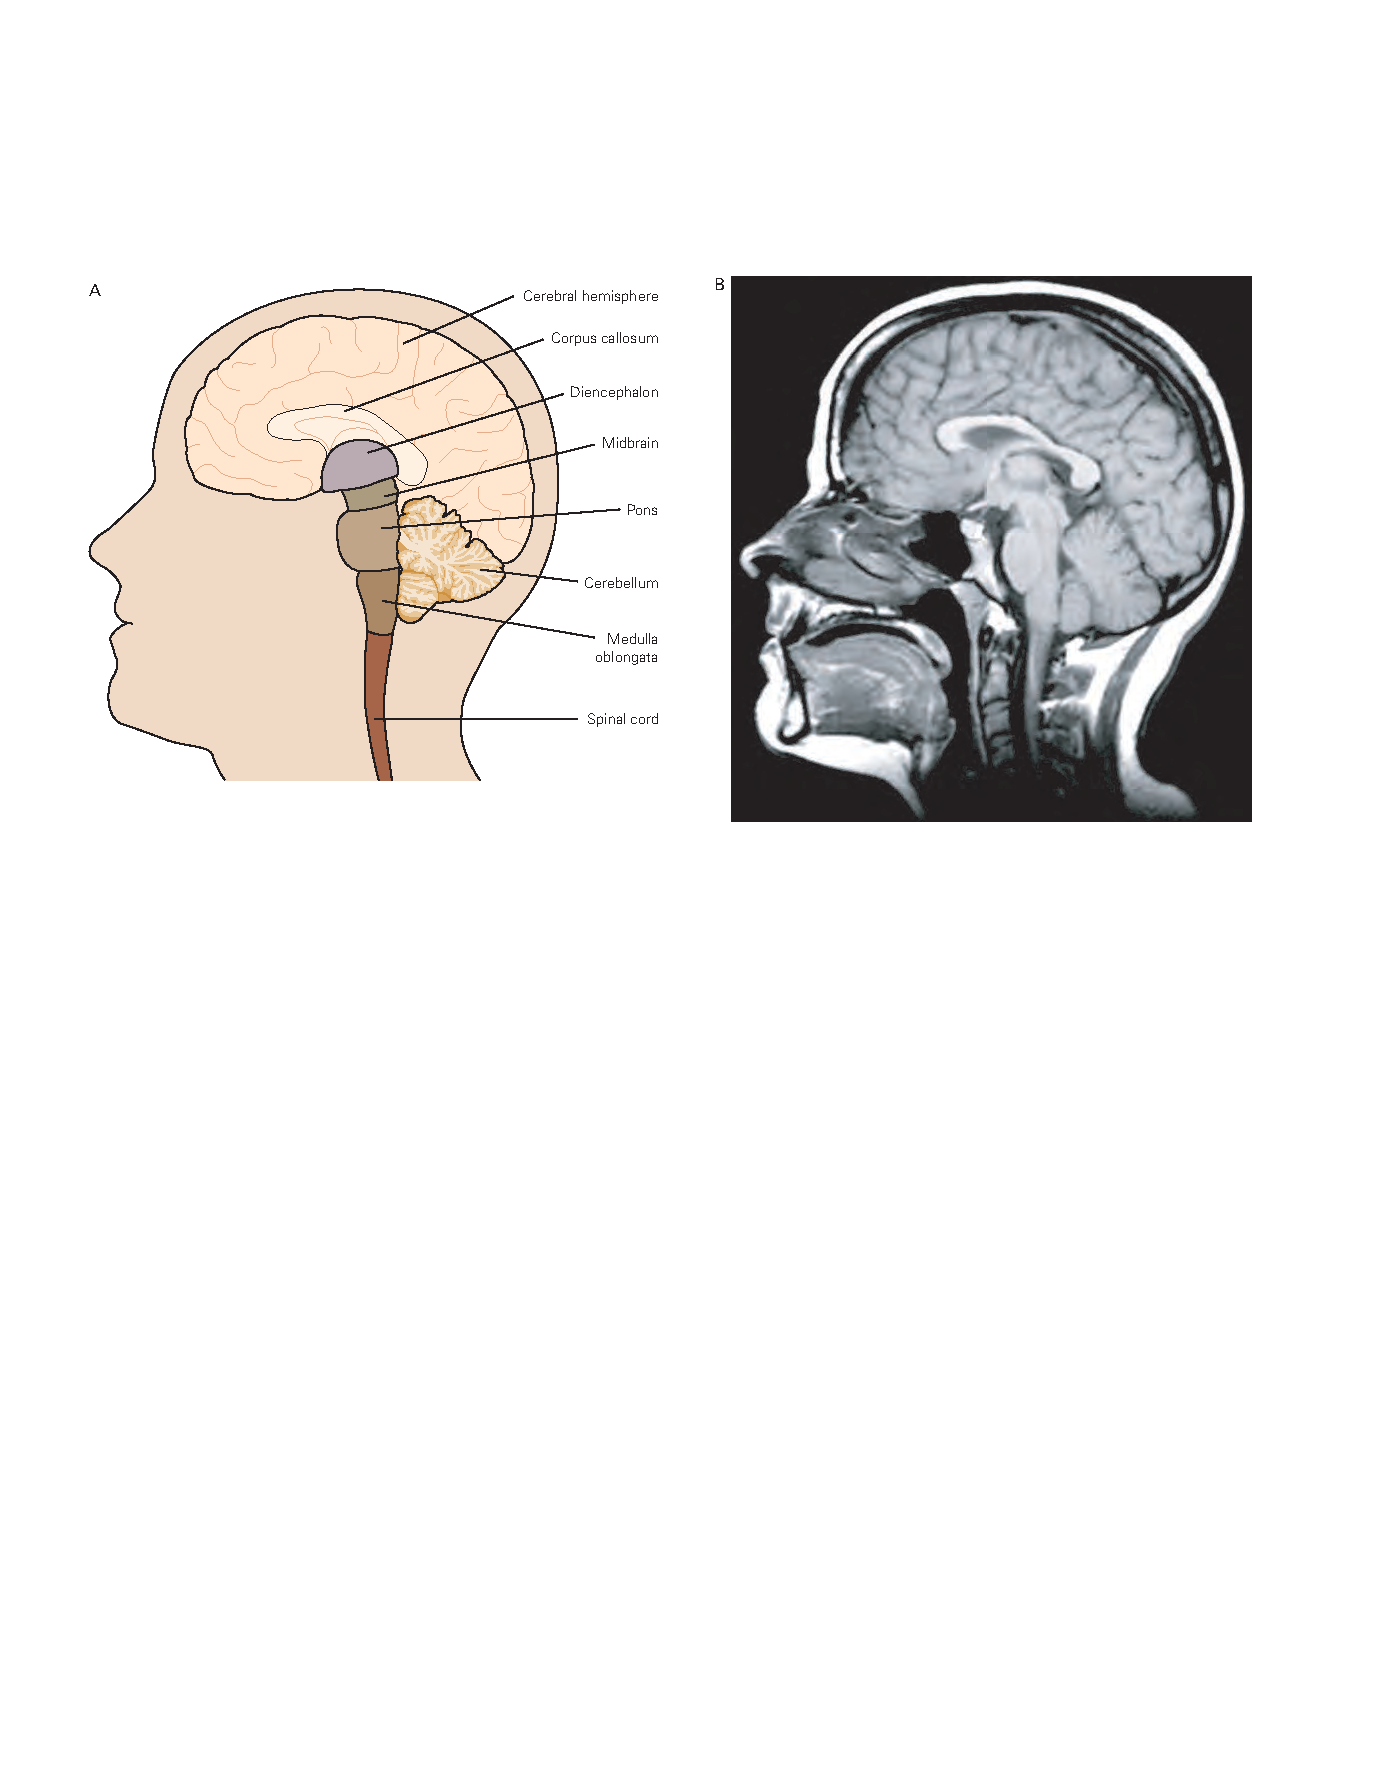
\includegraphics[width=0.9\linewidth]{chap01/fig_1_5}
	\caption{可以在活人的大脑中成像主要皮层和皮层下区域。
		\textbf{A.} 这张示意图显示了大脑的主要表面和深部区域,包括脊髓的延髓末端,以供参考。
		\textbf{B.} 在 A 部分绘制的主要大脑分区在活人脑的磁共振图像中很明显。}
	\label{fig:1_5}
\end{figure}


在每个半球中,覆盖的皮层分为四个叶,以覆盖它们的颅骨命名:额叶、顶叶、枕叶和颞叶(图~\ref{fig:1_3}B)。
每个叶都有几个特征性的深折叠,这是一种将一大片皮层包装到有限空间中的进化策略。
这些回旋的顶部称为脑回,中间的沟称为脑沟或裂隙。 
人与人之间非常相似的更突出的脑回和脑沟具有特定的名称。
例如,中央沟将中央前回(一个与运动功能有关的区域)与中央后回(一个处理感觉功能的区域)分开(图~\ref{fig:1_3}B)。
如第~\ref{chap:chap6}~章所述,无论是在死后组织中(图~\ref{fig:1_4}),还是实际上使用磁共振成像(图~\ref{fig:1_5}),几个突出的脑回仅在两个半球之间的内侧表面可见(图~\ref{fig:1_3}C),其他脑回位于脑裂和脑沟深处,因此只有在大脑被切片时才可见。


每个叶都有专门的功能。
额叶主要与短期记忆、计划未来行动和控制运动有关;
顶叶介导躯体感觉,形成身体形象并将其与个人以外的空间联系起来;
枕叶与视力有关;
颞叶处理听觉、物体和面孔的识别,以及通过其深层结构、海马体和杏仁核处理学习、记忆和情感。


两个重要特征表征了大脑皮层的组织。
首先,每个半球主要关注身体对侧(对侧)的感觉和运动过程。
因此,从身体左侧到达脊髓的感觉信息在到达大脑皮层的途中穿过神经系统的右侧。
同样,右半球的运动区控制着身体左半边的运动。
第二个特征是两个半球虽然外观相似,但在结构或功能上并不完全对称。



\section{认知能力本地化的第一个有力证据来自语言障碍研究}

大脑皮层中第一个被确定为对认知很重要的区域是与语言有关的区域。
这些发现来自对失语症的研究,失语症是一种语言障碍,最常发生在大脑组织的某些区域因中风、供应大脑半球一部分的血管闭塞或破裂而受损时。
失语症研究中的许多重要发现
在 19 世纪下半叶,接二连三地出现许多重要的失语症研究。
总而言之,这些进展构成了人类行为神经科学研究中最激动人心和最重要的章节之一。


法国神经学家布罗卡是第一个确定与语言有关的大脑特定区域的人。
\textit{布洛卡}受到\textit{加尔}绘制大脑高级功能图的影响,但他没有将行为与头骨上的肿块相关联,而是将失语症的临床证据与死后发现的脑损伤相关联。
1861 年,他写道:“我曾认为,如果有一门颅相学,那将是(大脑皮层中)回旋的颅相学,而不是(头上的)肿块的颅相学。” 
基于这种洞察力,布罗卡创立了神经心理学,这是一门心理过程的经验科学,他将其与加尔的颅相学区分开来。


1861 年,布罗卡描述了一位名叫勒博涅的病人,他由于中风而无法说话,尽管他能很好地理解语言。
该患者没有影响其说话能力的舌头、嘴巴或声带运动缺陷。
事实上,他可以毫无困难地说出孤立的单词、吹口哨和唱出一段旋律。
但他不能按语法说话或造出完整的句子,也不能用书面表达思想。
对这名患者的大脑进行的尸检显示,左额叶后下方区域有一个病变,现在称为布罗卡区(图~\ref{fig:1_6})。
\textit{布洛卡}研究了 8 名相似的患者,均在该区域有病变,并且每个病例的病变都位于左侧大脑半球。
这一发现促使\textit{布洛卡}在 1864 年宣布:“Nous parlons avec l’hémisphère gauche!” (我们用左半球说话!)。


\begin{figure}[htbp]
	\centering
	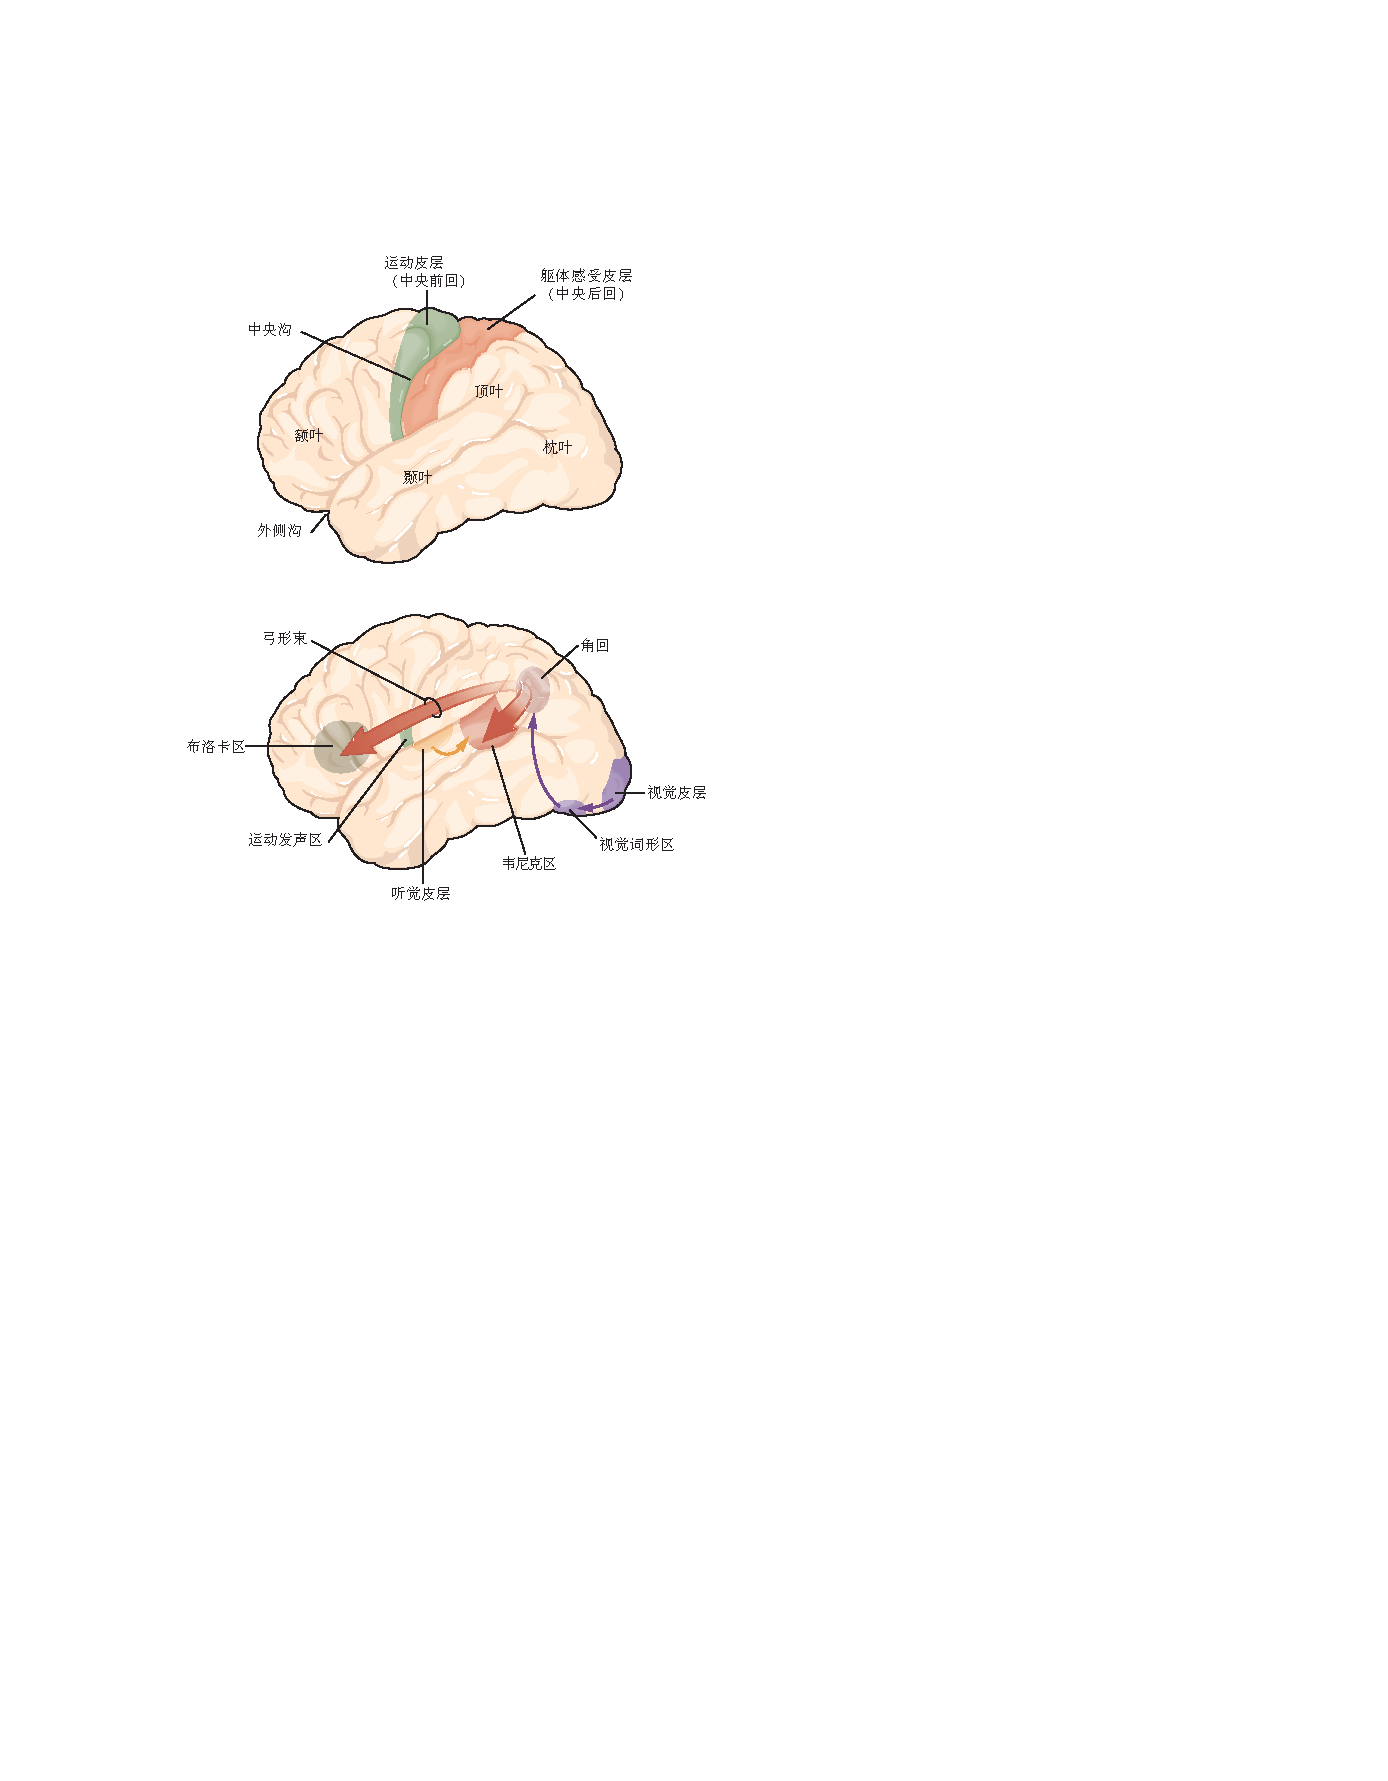
\includegraphics[width=0.6\linewidth]{chap01/fig_1_6}
	\caption{语言处理涉及左脑半球的几个区域。
		布洛卡区控制言语的产生。
		它位于控制形成单词的嘴巴和舌头运动的运动区附近。
		韦尼克区处理语言的听觉输入,对理解言语很重要。
		它位于初级听觉皮层和角回附近。
		法国神经学家\textit{朱尔斯$\cdot$代热林}在 1890 年代提出,角回中的多模态感觉区域整合了来自视觉和听觉的信息来表示单词,但最近的研究表明更多的腹侧枕颞皮层区域用于处理视觉单词。
		\textit{韦尼克}区通过双向通路与\textit{布洛卡}区相通,其中一部分由弓状束组成\cite{geschwind1979specializations}。}
	\label{fig:1_6}
\end{figure}


布洛卡的工作激发了人们对与其他特定行为相关的皮层部位的搜索——搜索很快就得到了回报。
1870 年,\textit{古斯塔夫$\cdot$弗里奇}和\textit{爱德华$\cdot$希茨格}表明,可以通过电刺激中央前回的离散区域来产生狗的特征性肢体运动,例如伸出爪子,这激起了科学界的热潮。
这些区域总是位于对侧运动皮层。
因此,最常用于书写和熟练动作的右手是由左半球控制的,而左半球也控制着说话。
因此,对大多数人来说,左半球被认为是主导的。


下一步是由\textit{韦尼克}于 1876 年采取的,他在 26 岁时发表了一篇现在已成为经典的论文,“失语症的综合症状:解剖学基础上的心理学研究”。
在其中,他描述了另一种类型的失语症,这是一种理解障碍而不是言语障碍:一种与表达障碍相反的接受障碍。
布罗卡的病人可以理解语言但不会说话,而韦尼克的病人可以造词但不能理解语言,只能说出毫无意义但合乎语法的句子。
而且,这种新型失语症的发生部位与布罗卡所描述的不同。
病变发生在大脑皮层后部,即颞叶与顶叶交汇处(图~\ref{fig:1_6})。


基于这一发现以及\textit{布洛卡}、\textit{弗里奇}和\textit{希茨格}的工作,\textit{韦尼克}制定了一种语言神经模型,试图调和和扩展当时大脑功能的主流理论。
颅相学家和细胞联结主义者认为,大脑皮层是功能特定区域的马赛克,而整体聚合场学派则声称,每一种心理功能都涉及整个大脑皮层。
韦尼克提出,只有最基本的心理功能,即与简单的知觉和运动活动有关的功能,才完全由皮层离散局部区域的神经元调节。
他认为,更复杂的认知功能是由几个功能部位之间的相互联系产生的。
通过将局部功能原理整合到联结主义框架中,韦尼克强调了单一行为的不同组成部分可能在大脑的多个区域中得到处理的观点。
因此,他是第一个提出分布式处理思想的人,分布式处理现在是神经科学的核心原则。


\textit{韦尼克}假设语言涉及独立的运动和感觉程序,每个程序都由不同的皮层区域控制。
他提出,控制言语嘴部运动的运动程序位于\textit{布罗卡区},恰好位于控制嘴、舌、上颚和声带的运动区的前面(图~\ref{fig:1_6})。
接下来,他将控制单词感知的感觉程序分配到他发现的颞叶区域,现在称为韦尼克区。
该区域被听觉皮层和现在统称为联合皮层的区域包围,这些区域整合了听觉、视觉和躯体感觉。
根据\textit{韦尼克}的模型,这两个语言中心之间的交流是通过一大束被称为弓状束的轴突来调节的。


因此,韦尼克制定了第一个连贯的语言神经模型,该模型在第~\ref{chap:chap55}~章中进行了重要的修改和阐述,至今仍然有用。
根据这个模型,口语或书面词的神经处理开始于专门负责听觉的皮层的单独感觉区域 或视觉信息。
然后,通过中间关联区域提取适合口头或书面文字识别的特征,将此信息传送到韦尼克区,在那里它被识别为语言并与意义相关联。


韦尼克模型的强大之处不仅在于它的完整性,还在于它的预测效用。
该模型正确预测了第三种类型的失语症,一种由断开连接引起的失语症。
在这种类型中,语言的感受区和表达区完好无损,但连接它们的神经纤维(弓状束)被破坏。
这种传导性失语症,正如现在所称,其特征是频繁的、基于声音的言语错误(音素性错语)、重复困难和言语工作记忆的严重限制。
传导性失语症患者能理解他们听到和读到的单词,并且在说话时没有运动障碍。
然而,他们无法连贯地说话; 他们省略部分单词或替换不正确的声音,并且在逐字重复他们听到、读到或从记忆中回忆起的多音节单词、短语或句子时遇到很大困难。
尽管他们痛苦地意识到自己的错误,但他们连续不断的自我纠正尝试往往都没有成功。


在解剖学家布罗德曼的领导下,部分受到韦尼克的启发,20 世纪初在德国出现了一个新的皮层定位学派,该学派根据细胞的形状及其分层的变化来区分皮层的功能区域 安排。
使用这种细胞构造方法,布罗德曼区分了人类大脑皮层中 52 个解剖学和功能上不同的区域(图~\ref{fig:1_7})。


\begin{figure}[htbp]
	\centering
	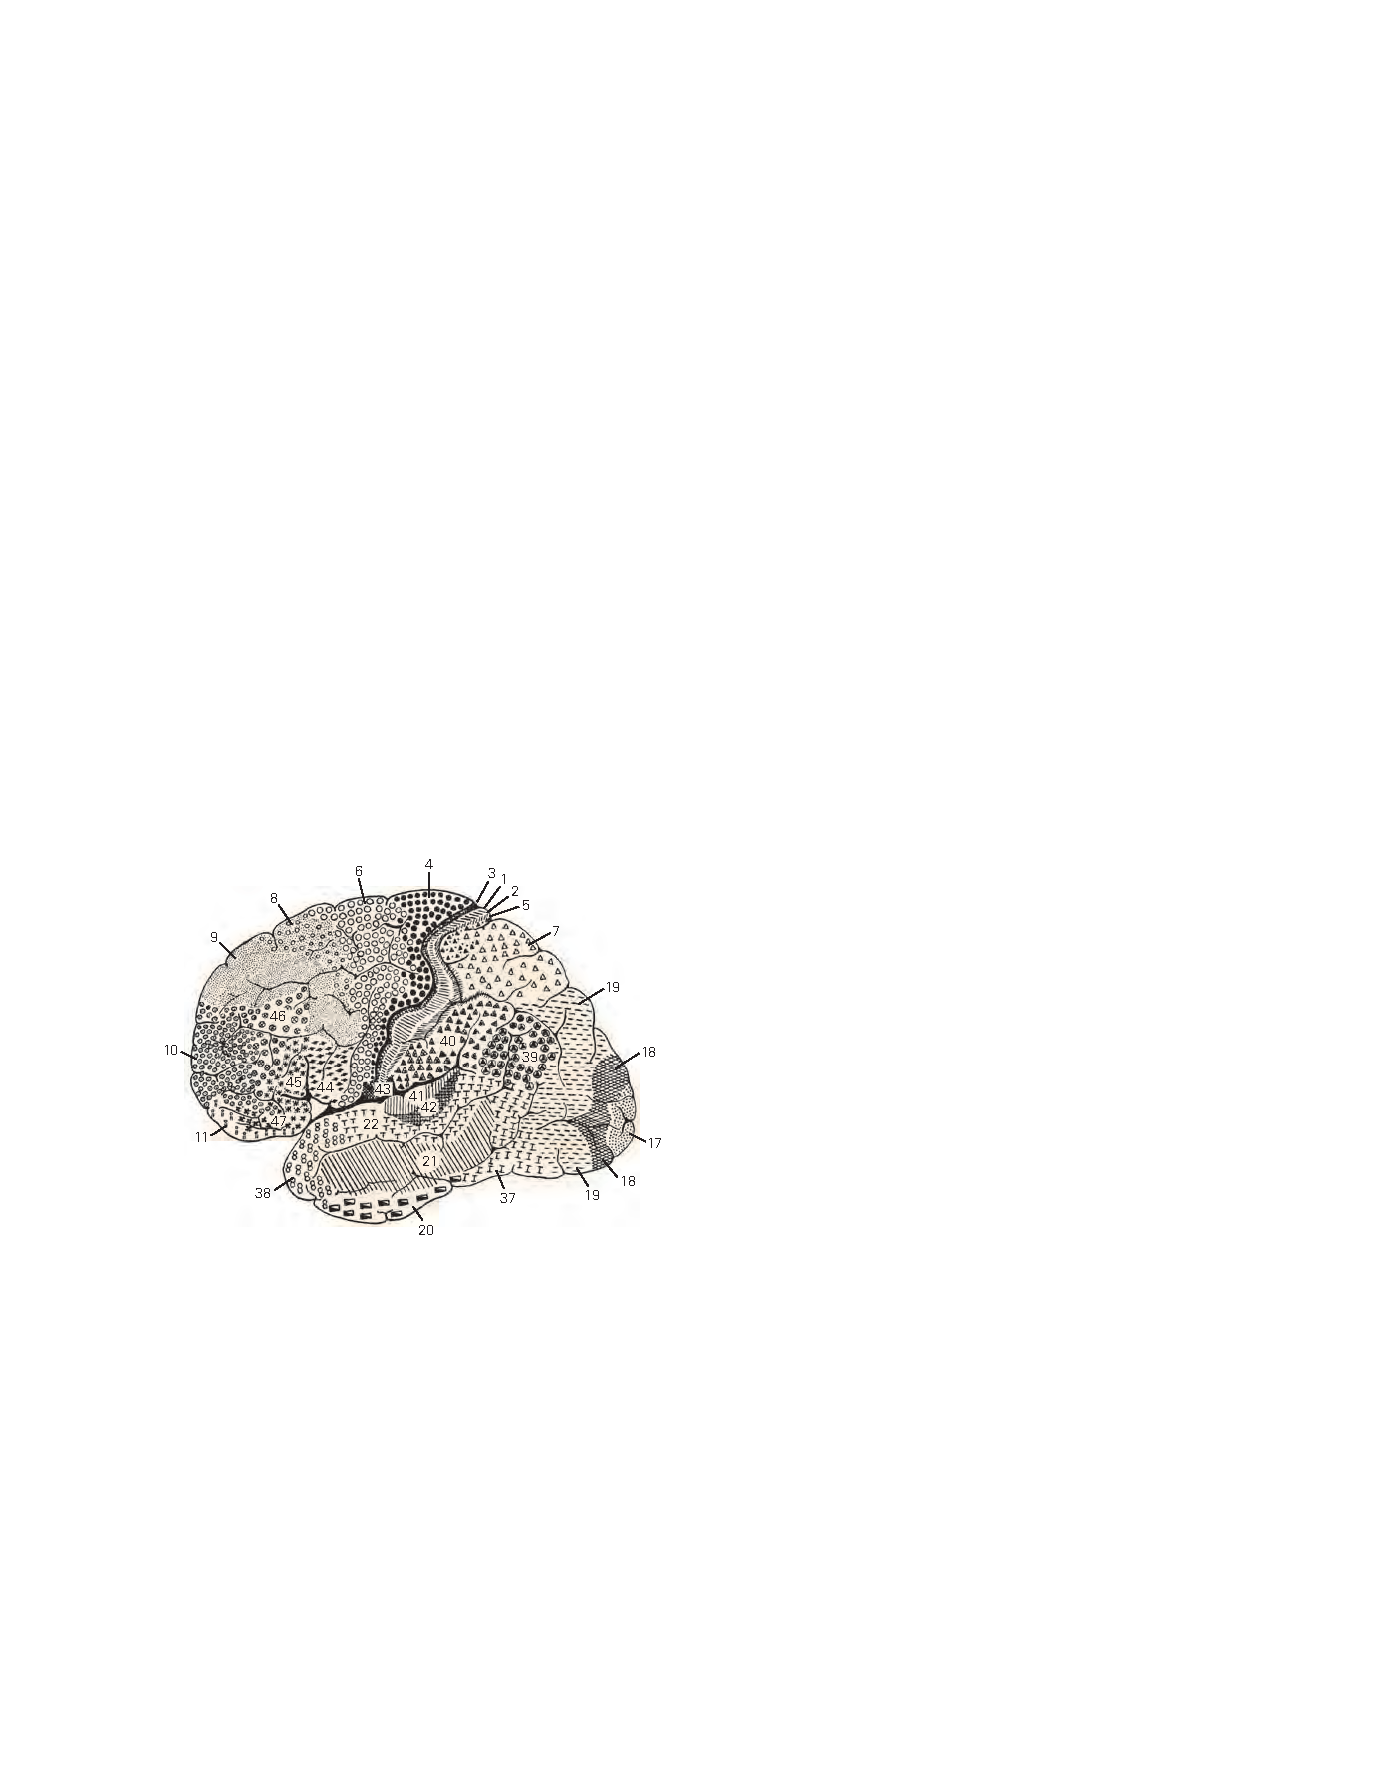
\includegraphics[width=0.6\linewidth]{chap01/fig_1_7}
	\caption{20 世纪初,人类大脑皮层被分为 52 个独立的功能区。
		显示的区域是由解剖学家布罗德曼根据独特的神经细胞结构和细胞层的特征排列确定的。
		该方案至今仍在广泛使用,并不断更新。
		布罗德曼定义的几个区域被发现可以控制特定的大脑功能。
		例如,区域 4 是运动皮层,负责随意运动。
		区域 1、2 和 3 构成初级体感皮层,主要从皮肤和关节接收感觉信息。
		第 17 区是初级视觉皮层,它接收来自眼睛的感觉信号并将它们传递到其他区域以进行进一步处理。
		区域 41 和 42 构成初级听觉皮层。
		该图仅显示了皮层外表面的可见区域。}
	\label{fig:1_7}
\end{figure}


尽管大脑皮层功能离散区域的生物学证据令人信服,但到 20 世纪初,大脑的整体观点一直主导着实验思维和临床实践,直到 1950 年。
这种令人惊讶的事态在很大程度上要归功于几位著名的神经科学家,他们 主张整体观的有英国神经学家亨利海德、俄国行为生理学家伊万巴甫洛夫和美国心理学家卡尔\textit{拉什利}。


最有影响力的是\textit{拉什利},他对用细胞构造方法来绘制皮层功能图深表怀疑。
“‘理想’的建筑地图几乎一文不值,”\textit{拉什利}写道。
“区域划分在很大程度上在解剖学上毫无意义,并且对皮层的假定功能划分具有误导性。” 
他对各种脑损伤对老鼠学习走迷宫能力的影响的研究进一步强化了他的怀疑态度。
从这些研究中,\textit{拉什利}得出结论,学习缺陷的严重程度取决于损伤的大小,而不是其精确位置。
失望的\textit{拉什利}——以及他之后的许多其他心理学家——得出结论,学习和其他高级心理功能在大脑中没有特殊的位置,因此不能归因于特定的神经元集合。


根据他的观察,\textit{拉什利}通过进一步最小化单个神经元、特定神经元连接,甚至特定大脑区域在特定行为中产生的作用,重新制定了聚合场观点。
根据\textit{拉什利}的质量作用理论,对记忆等功能至关重要的是大脑的整体质量,而不是其局部成分。


\textit{拉什利}的老鼠实验现在被重新诠释。
各种研究表明,\textit{拉什利}使用的迷宫学习不适合寻找局部皮层功能,因为它涉及太多的运动和感觉能力。
被剥夺了一种感觉能力,比如视觉,老鼠仍然可以学会使用触觉或嗅觉走迷宫。
此外,正如我们将在本书后面看到的那样,许多心理功能是由不止一个区域或神经元通路调节的。
因此,一个给定的功能可能不会被单个损伤消除。
在考虑大脑的认知功能时,这一点尤为重要。
例如,空间知识得到许多顶叶关联区域的支持,这些关联区域将视觉与注视的潜在移动、头部的转动、手的伸展等联系起来。
原则上,这些关联区域中的任何一个都可以补偿另一个关联区域的损伤。
对顶叶的严重损伤会导致明显的空间知识缺陷(空间失认症)(第~\ref{chap:chap59}~章)。
这样的观察似乎支持群众行动理论,但我们现在认识到它与包含功能冗余概念的功能定位相容。


很快,功能定位的证据变得势不可挡。
从 1930 年代后期开始,英国的\textit{埃德加$\cdot$阿德里安}和美国的\textit{韦德$\cdot$马歇尔}和\textit{菲利普$\cdot$巴德}发现,触摸猫身体的不同部位会引起大脑皮层不同区域的电活动。
通过系统地探测体表,他们在\textit{布罗德曼}描述的大脑皮层特定区域建立了体表的精确图谱。
这一结果表明,可以根据解剖学标准(例如细胞类型和细胞分层、细胞连接,以及最重要的行为功能)明确定义功能不同的皮层区域。
正如我们将在后面的章节中看到的那样,功能特化是大脑皮层的一个关键组织原则,甚至延伸到皮层区域内的单个细胞列。
事实上,大脑被划分为比布罗德曼设想的更多的功能区域。


更精细的方法使我们有可能更多地了解与语言有关的不同大脑区域的功能。
在 20 世纪 50 年代后期,\textit{怀尔德$\cdot$潘菲尔德}和后来的\textit{乔治$\cdot$奥杰曼}重新研究了对产生语言至关重要的皮层区域。
在癫痫脑部手术期间进行局部麻醉时,清醒的患者被要求命名物体(或以其他方式使用语言),同时用小电极刺激暴露皮层的不同区域。
如果大脑皮层的某个区域对语言至关重要,则电刺激的应用会阻止患者命名物体的能力。
通过这种方式,\textit{潘菲尔德}和\textit{奥杰曼}能够确认 布洛卡和韦尼克描述的大脑皮层的语言区域。
正如我们将在第~\ref{chap:chap55}~章中了解到的那样,语言神经网络比布洛卡和韦尼克所描述的神经网络广泛和复杂得多。


最初,几乎所有关于语言解剖结构的知识都来自对脑部病变患者的研究。
今天,\textit{功能性磁共振成像}和其他非侵入性方法可以对从事阅读、说话和思考的健康人进行分析(第~\ref{chap:chap6}~章)。
\textit{功能性磁共振成像}不仅证实了阅读和说话会激活不同的大脑区域,而且还揭示了在没有感觉输入的情况下仅仅思考一个词的含义会激活左额叶皮层中一个仍然不同的区域。
事实上,即使在传统语言领域内,各个子区域也会在不同程度上被吸收,这取决于我们思考单词、表达单词以及从其他单词的排列(即句法)中解析它们的含义的方式。
新的成像工具承诺不仅会告诉我们涉及哪些领域,还会揭示它们相互联系的功能逻辑。


现代方法论带来的巨大惊喜之一是,大脑皮层的如此多区域在语言理解和产生过程中都被激活了。
这些包括左半球的传统语言区域,由\textit{布洛卡}、\textit{韦尼克}和\textit{代热林}确定; 它们在右半球的同系物;
和新确定的区域。
功能成像倾向于阐明不同募集的区域,而来自中风、肿瘤或损伤的损伤区分对一种或多种功能至关重要的大脑区域。
因此,曾经被认为专门负责语言生成的布罗卡区似乎也参与了包括理解在内的各种语言任务(图~\ref{fig:1_6})。
在某些情况下,功能成像需要对病变研究确定的关键区域进行改进或修正。
例如,除了顶叶皮层的角回之外,阅读现在被认为可以募集腹侧枕颞皮层的专门区域(如图~\ref{fig:1_6} 所示)。


因此,大脑中语言的处理不仅体现了局部功能原则,而且体现了这一原则的更复杂的阐述,即许多具有专门功能的不同神经结构属于系统。
也许这是关于本地化和分布式过程的争论的自然调和——即少数不同的区域,每个区域都具有一小组功能,并通过它们的相互作用对感知、行动和观念的现象学做出贡献。
大脑分工的任务可能与我们的直觉告诉我们的不同。
谁会猜到对一个物体的运动和颜色的神经分析会发生在不同的通路中,而不是一个单一的通路来调解对物体的统一感知?
同样,我们可能期望语言的神经组织可能不完全符合通用语法理论的公理,但支持语言理论描述的非常无缝的功能。


对脑损伤患者的研究继续提供重要的洞察力,以了解大脑是如何组织语言的。
最令人印象深刻的结果之一来自对聋人的研究,他们在遭受脑损伤后失去了使用手语(例如,\textit{英国手语}或\textit{美国手语})进行交流的能力。
手语使用手部动作而不是发声,并且通过视觉而不是声音来感知,但具有与口语相同的结构复杂性。
与口语处理一样,手语处理位于左半球。 左半球的损伤会对手语产生非常特殊的影响,就像口语一样,会影响手语理解(韦尼克区受损后)、语法或流畅性(布罗卡区受损后)。
这些临床观察得到功能性神经影像学的支持。
毫不奇怪,手语和口语的产生和理解并不涉及相同的大脑区域,但重叠确实很显着(图~\ref{fig:1_8})。
甚至有证据表明,处理符号的组成部分(例如,使用的手形)涉及的一些相同大脑区域在对语音进行押韵判断时涉及。


\begin{figure}[htbp]
	\centering
	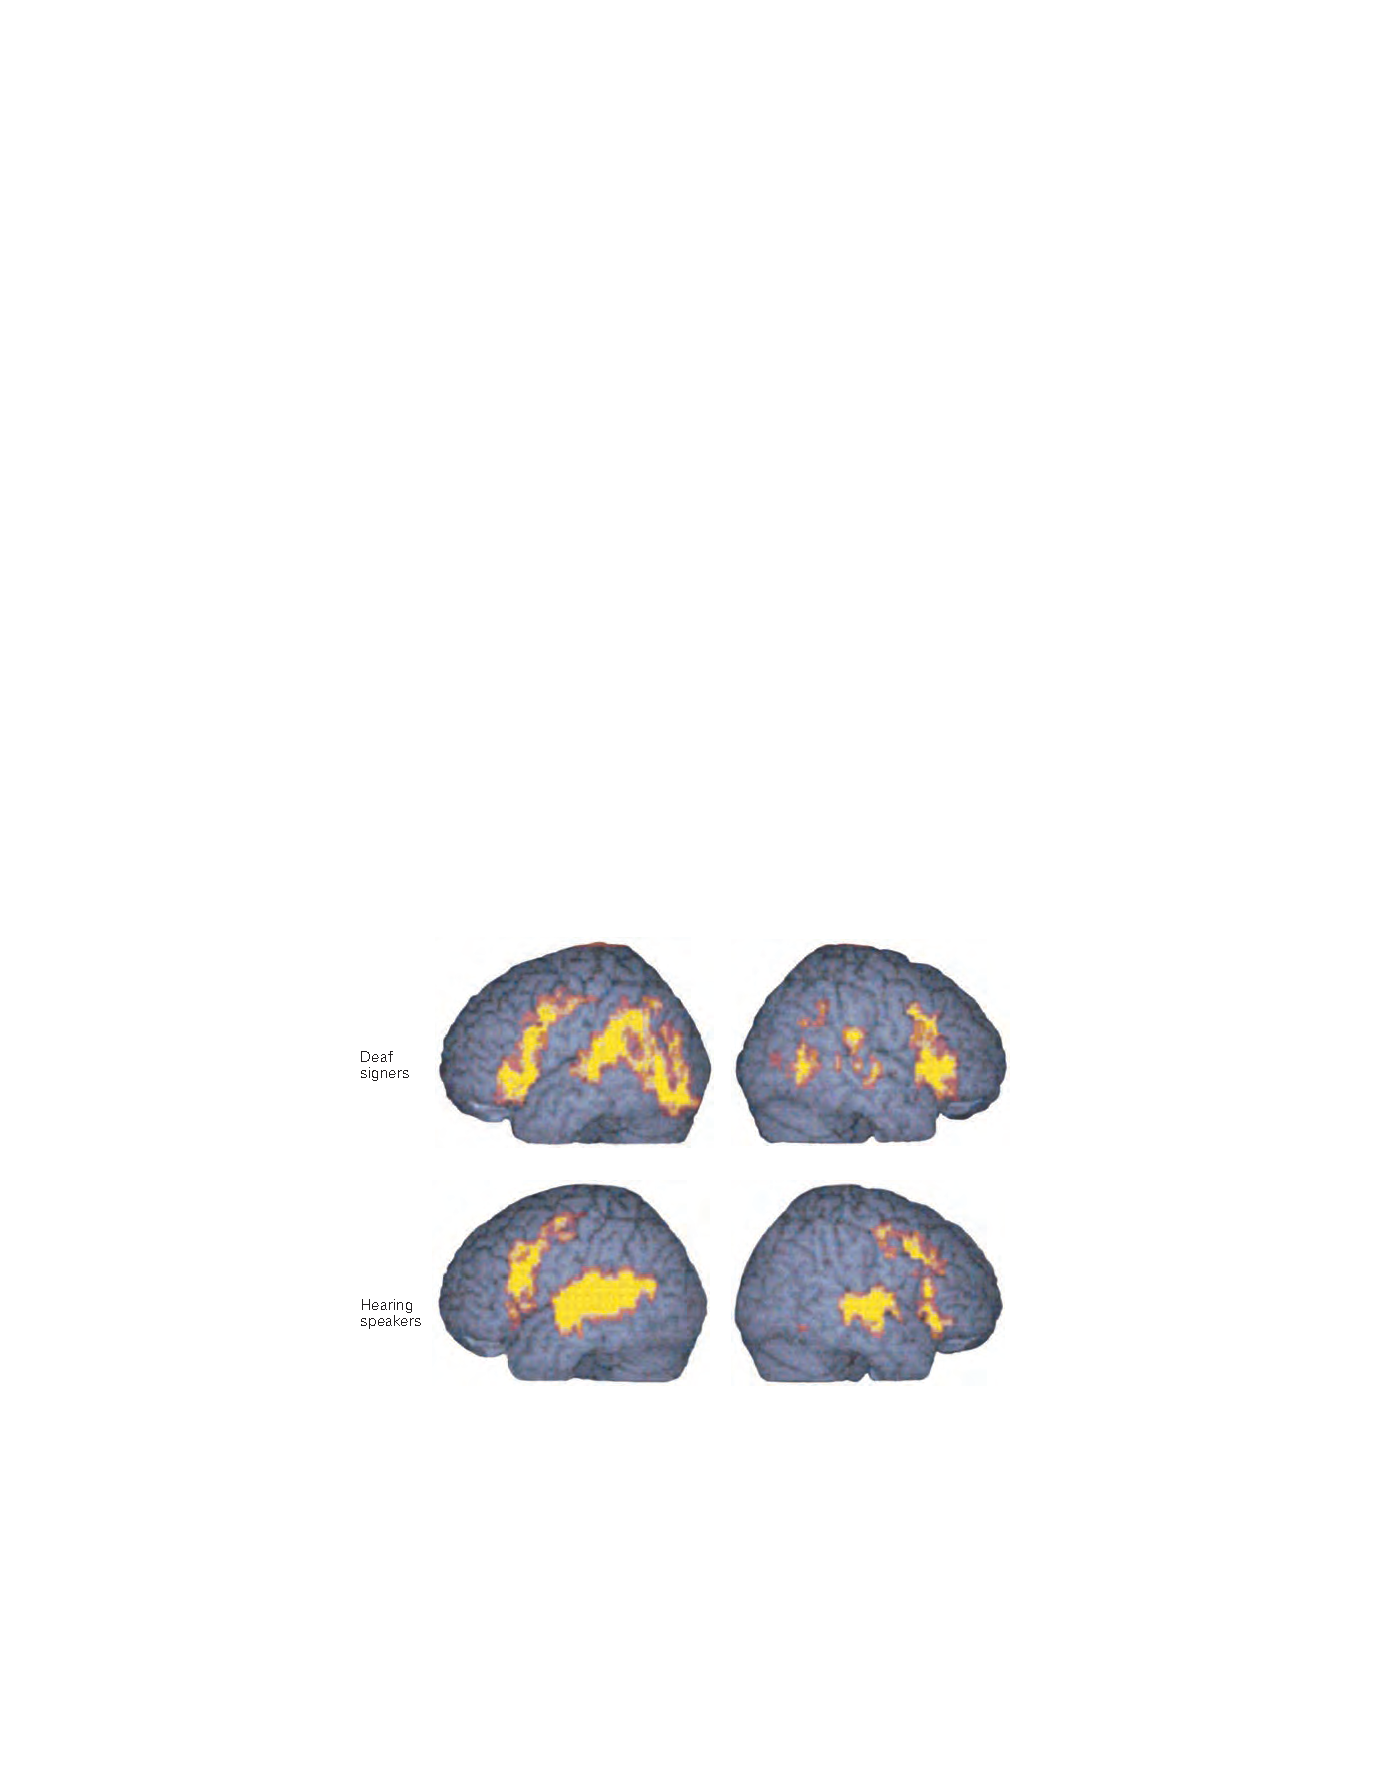
\includegraphics[width=0.75\linewidth]{chap01/fig_1_8}
	\caption{手语聋人和听力正常的人共享共同的语言处理区域。
		大脑皮层中涉及口语或手语识别的区域,通过\textit{功能性磁共振成像}识别。
		黄色高亮显示左右大脑半球(分别为左列和右列)在理解语言时比在执行感知任务时更活跃的区域。
		对于失聪手语者(顶行),突出显示的区域在理解英国手语期间比在检测叠加在同一静止手语者身上的视觉刺激期间更加活跃。
		对于有听力的说话者(下排),在理解视听语音期间突出显示的区域比在观看静止(无声)说话者时检测音调期间更活跃\cite{macsweeney2002neural}。}
	\label{fig:1_8}
\end{figure}


这些观察说明了三点。
首先,语言处理主要发生在左半球,与处理语言中使用的感觉和运动方式的通路无关。
其次,听觉输入对于左半球语言能力的出现和运作不是必需的。
第三,口语只是左半球调节的一系列语言技能之一。


对其他行为的调查为大脑具有不同认知系统的观点提供了额外的支持。
这些研究表明,复杂的信息处理需要许多相互关联的皮层和皮层下区域,每个区域都涉及处理感觉刺激或运动的特定方面,而不是其他方面。
例如,对物体位置、大小和形状的知觉意识依赖于许多顶叶联合区域的活动,这些区域将视觉与潜在的动作联系起来,例如移动眼睛、调整头部方向、伸手和调整手的形状以进行抓握。
顶叶区域不会启动这些动作,但会将感觉信息评估为与这些潜力相关的证据。
它们从背侧视觉流(有时称为\textit{空间通路},但更恰当地称为 how 通路)接收信息,以构建关于物体位置和其他空间特性的知晓状态。
腹侧视觉流,或什么通路,也与可能的行动有关,但这些与社交和觅食有关。
这些联想建立了对物体、面孔、食物和潜在伴侣的可取性的认知。
从这个意义上说,\textit{内容通路}也可能是 how 途径。



\section{心理过程是大脑中基本处理单元之间相互作用的产物}

大脑功能定位的证据在过去常常被拒绝,原因有很多,这些证据回想起来似乎如此明显和令人信服。
颅相学家在没有充分证据的情况下以夸张的形式引入了定位的概念。
他们把大脑皮层的每个区域都想象成一个独立的精神器官,专门负责人格完整而独特的方面,就像胰腺和肝脏是独立的消化器官一样。
\textit{弗卢龙}对颅相学的拒绝以及随之而来的聚集场观点的支持者(反对定位)和细胞连接主义者(支持定位)之间的争论是对一种简单化且没有足够实验证据的理论的回应。


在韦尼克发现大脑中语言的模块化组织(具有独特功能的互连节点)之后,我们现在认为所有认知能力都是分布在大脑多个区域的许多处理机制相互作用的结果。
也就是说,特定的大脑区域并不完全负责特定的智力,而是共同发挥作用的基本处理单元。
感知、运动、语言、思想和记忆都是通过这些区域内离散大脑区域(计算模块)中串行和并行处理的相互联系而成为可能的。
因此,单个区域的损伤不一定会像许多早期神经学家认为的那样导致认知功能(或能力)的完全丧失。
即使一种行为最初消失了,它也可能部分恢复,因为大脑未受损的部分重新组织了它们的联系。
此外,当\textit{局灶性损伤}对心理功能产生不利影响时,它可能会通过破坏其他主要位点的功能(精神分裂症)而间接影响。
事实上,对这种性质的观察让韦尼克的学生库尔特戈德斯坦接受了更全面的观点。


因此,认为心理功能严格由一系列神经细胞和大脑区域调节是不准确的——每个神经细胞和大脑区域都直接连接到下一个——因为在这样的安排中,当单个连接受损时,整个过程就会中断。
一个更现实的比喻是一个过程,该过程由模块网络中的多个并行通路组成,这些通路相互作用并最终汇聚在一组共同的目标上。
网络中单个路径的故障可能会影响该路径携带的信息,而不会破坏整个系统。
网络的其余部分可能能够修改其性能以适应一条路径的故障。


大脑中的模块化处理被接受的速度很慢,因为直到最近,还很难证明哪些心理运算的组成部分是由特定大脑区域或通路传达的。
以导致可检验假设的方式定义心理操作也不容易。
然而,随着近几十年来现代认知心理学和脑科学的不断融合,我们已经开始意识到心理功能可以成功地分解为子功能。


为了说明这一点,请考虑我们如何学习、存储和回忆有关物体、人和事件的信息。
简单的反思表明,我们将每条知识存储为一个单一的表征,可以通过记忆慢跑刺激甚至仅通过想象力来回忆。
例如,你所知道的关于苹果的一切似乎都存储在一个完整的表征中,无论你看到一个特定的苹果、苹果的一部分、红苹果还是绿苹果、书面单词“苹果”,还是关于引力发现的虚构故事,都同样可以访问。
然而,我们的经验并不能忠实地指导知识是如何存储在记忆中的。


关于苹果的知识并没有存储为一个单一的连贯表征,而是被细分为不同的类别并单独存储。
大脑的一个区域存储着关于你拿苹果的方式、你对柔软度的感觉(与新鲜度有关)、颜色(与偏好或新鲜度相关)、你与他人交流苹果存在或味道的方式,以及它与计算机、物理学家、蠕虫、蛇和圣经花园的语义联系的信息。
“苹果”的概念包含了这些考虑因素中的每一个,还有更多。
一个自然的假设是,一个包含许多细节的连贯概念必须存在于大脑的一个单一位置;
然而,一个同样有效的假设是,像“苹果”这样的统一概念以各种神经结构之间的多重链接的形式存在于大脑中,每个神经结构都有一种特定的信息,通过记忆检索的动作进行协调。


心理过程模块化组织最惊人的例子是发现我们的自我意识——一个自我意识的存在,当我们说“我”时的意思总和——是通过我们大脑中独立回路的连接实现的 两个大脑半球,每个半球调节自己的意识。
\textit{罗杰$\cdot$斯佩里}、\textit{迈克尔$\cdot$加扎尼加}和 \textit{约瑟夫$\cdot$伯根}在研究患者的过程中做出了一个非凡的发现,即意识也不是一个单一的过程,这些患者的胼胝体——连接两个大脑半球的主要区域——被切断作为治疗癫痫。
他们发现每个半球都有一种独立于另一半球运作的意识。


因此,当一名患者左手拿着一本最喜欢的书阅读时,控制左手但在语言理解中只起次要作用的右半球发现,它从简单地看书获得的原始视觉信息是无聊的。
右半球命令左手放下书。
另一个病人会用左手穿上衣服,同时用另一只手脱下衣服。 每个半球都有自己的想法!
此外,优势半球有时会评论非优势半球的表现,经常表现出一种错误的自信感,因为它不知道解决方案是专门提供给非优势半球的。


这些发现将曾经属于哲学和精神分析领域的意识研究带入了神经科学的范畴。
正如我们将在后面的章节中看到的,本章中描述的许多问题在意识的神经理论中再次出现。
没有人质疑很多信息处理——也许是最大的份额——没有达到有意识的认识这一想法。
当感官信息、行动计划或想法确实成为意识时,神经科学试图解释调节这种转变的机制。
虽然目前还没有令人满意的解释,但一些脑科学家将这一过程比作注意力焦点的转移,由不同的神经元群介导,而另一些人则认为,意识需要在广泛分离的神经元区域之间的功能相互作用中发生质的变化。


我们花了这么长时间才弄清楚大脑的哪些区域介导了哪些心理活动,主要原因是我们正在处理生物学最深奥的谜题:解释意识和自我意识的神经机制。
目前还没有令人满意的理论来解释为什么只有一些到达我们眼睛的信息会导致对物品、人或场景的主观意识状态。 
我们知道,我们有意识地意识到我们思想思考的一小部分,而那些确实刺穿意识的想法必须来自大脑无意识地执行的步骤。
正如我们在第~\ref{chap:chap56}~章中提出的那样,一些意识之谜的答案可能比想象的更接近。


同时,我们目前理解上的差距也对神经科学提出了实际的认识论挑战。
在我们对知觉、行为和认知的描述中,我们不得不依赖我们对世界、身体和观念的有意识体验。
然而,在这样做时,我们冒着错误描述许多不穿透意识的心理过程的风险。
例如,我们倾向于用与感官信息的主观体验相一致的术语来描述知觉问题,而即使是复杂但无意识的知觉内容知识也可能与行为效用(可供性)有更大的相似性,实际上是对以下问题的回答 这是否是我可能会选择吃、坐在上面或进一步参与的东西。
同样,大脑执行推理、制定战略和决策等认知过程的方式可能与我们从有意识的深思熟虑中推断出的步骤大致相似。


这些警示说明有一个明显的推论。
许多认知功能在没有意识的情况下发生的洞察力提出了这样一种可能性,即在研究更基本的行为时揭示的神经科学原理可以提供对更复杂的认知过程的洞察力。
受过训练以执行复杂任务的动物大脑的神经记录导致了对认知过程的理解,例如决策、推理、计划和分配注意力。 
这些实验模型经常外推到人类功能,并且在它们不足的地方,它们激发了新的假设。
通常情况下,即使不能从我们理解的空白中收集到洞察力,也会有灵感。


要分析大脑如何产生特定的心理过程,我们不仅必须确定该过程的哪些方面取决于大脑的哪些区域,还必须确定相关信息的表示、路由和转换方式。
现代神经科学试图整合这种跨多个尺度的理解。
例如,在单个神经细胞及其分子成分水平上的研究阐明了电兴奋性和突触连接的潜在机制。
对细胞和简单回路的研究有助于深入了解神经计算,从基本操作(如控制网络激励)到更精湛的计算专长(如从原始感官数据中获取有意义的信息)。
研究回路和大脑区域之间的相互作用可以解释我们如何协调广泛分离的肌肉群或表达对命题的信念。
所有这些层次的知识都通过数学形式化、计算机模拟和心理学理论结合在一起。
这些概念工具现在可以与现代生理学技术和大脑成像方法相结合,从而可以跟踪活体动物和人类实时进化的心理过程。
事实上,今天神经科学的兴奋源于这样一种信念,即构成人类思想和行为基础的生物学原理在我们的掌握之中,并且可能很快就会被用来阐明和改善人类状况。




\section{亮点}

1. 神经科学试图在多个组织层次上理解大脑,从细胞及其成分到思维的运作。


2. 神经科学的基本原理连接了时间、复杂性和状态的各个层次——从细胞到行动和思想,从通过学习的发展到专业知识和遗忘,从正常功能到神经缺陷和恢复。
第一步,必须了解构建块——神经细胞的电特性及其与其他神经细胞的连接——以及从支持细胞到通路的神经系统组织。


3. 神经元学说指出,单个神经细胞(神经元)是神经系统的基本组成部分和信号元件。


4. 神经元被组织成具有专门功能的回路。
最简单的回路调节反射;
更复杂的认知功能需要更复杂的回路。
这种组织原则将神经元学说扩展到细胞连接主义。


5. 即使在复杂的回路中,关键节点也可以被识别为与特定功能相关的区域。
大脑功能定位的第一个明确证据来自对语言产生特定障碍的研究。


6、两个大脑半球从身体的对侧接收信息,控制对侧的动作。


7. 虽然大脑功能定位原理优于其主要的历史替代方案——聚合场和质量作用理论——但它正在不断完善。
大脑皮层的任何区域都不能独立于其他皮层和皮层下结构而发挥作用。


8. 本地化的一个主要改进是模块化功能组织的原则。
大脑包含许多信息表征,这些信息既由特定计算的某些特征的相关性组织,也由这些信息的各种用途组织。
这是一种关于目的或潜在行动的冗余形式。


9. 脑科学的未来需要整合跨越传统学科界限的思想。
我们必须对各种各样的资源敞开心扉,以指导我们的直觉和研究策略,从\textit{意识的崇高本质}到看似平凡的\textit{全身麻醉对丘脑周围细胞环中钙传感器的作用}。


\chapter{基因和行为} \label{chap:chap2}

所有行为都是由基因和环境的相互作用塑造的。
简单动物的大多数刻板行为都受到环境的影响,而人类高度进化的行为则受到基因指定的先天特性的限制。
基因不直接控制行为,但基因编码的\textit{核糖核酸}和蛋白质会在不同时间和多个层面发挥作用,影响大脑。
基因指定了组装大脑的发育程序,并且对于神经元、神经胶质细胞和突触的特性至关重要,这些特性使神经元回路发挥作用。
代代稳定遗传的基因创造了新体验可以在学习过程中改变大脑的机制。


在本章中,我们将探讨基因如何影响行为。
我们首先概述基因确实影响行为的证据,然后回顾分子生物学和遗传传递的基本原理。
然后,我们提供了遗传对行为影响的记录方式的示例。
通过对蠕虫、苍蝇和老鼠的研究,人们对基因调节行为的方式有了深刻的了解,这些动物的基因组可用于实验操作。
通过对人类大脑发育和功能的分析,基因和人类行为之间出现了许多有说服力的联系。
尽管研究人类复杂特征存在固有的巨大挑战,但最近的进展已经开始揭示神经发育和精神综合症(如自闭症、精神分裂症和双相情感障碍)的遗传风险因素,为阐明基因、大脑和行为。



\section{了解\textit{分子遗传学}和遗传率对研究人类行为至关重要}

许多人类精神疾病和神经系统疾病都有遗传因素。
患者的亲属比一般人群更容易患上这种疾病。
遗传因素对群体特性的影响程度称为\textit{遗传力}。
遗传力最强的案例是基于双胞胎研究,1883 年\textit{弗朗西斯$\cdot$高尔顿}首次使用了同卵双胞胎。
这样的同卵双胞胎共享所有基因。
相反,异卵双胞胎是由两个不同的受精卵发育而来的;
这些异卵双胞胎与正常的兄弟姐妹一样,平均共享一半的遗传信息。
多年来的系统比较表明,同卵双胞胎在神经和精神特征方面往往比异卵双胞胎更相似(一致),这为这些特征的可遗传成分提供了证据(图~\ref{fig:2_1}A)。


\begin{figure}[htbp]
	\centering
	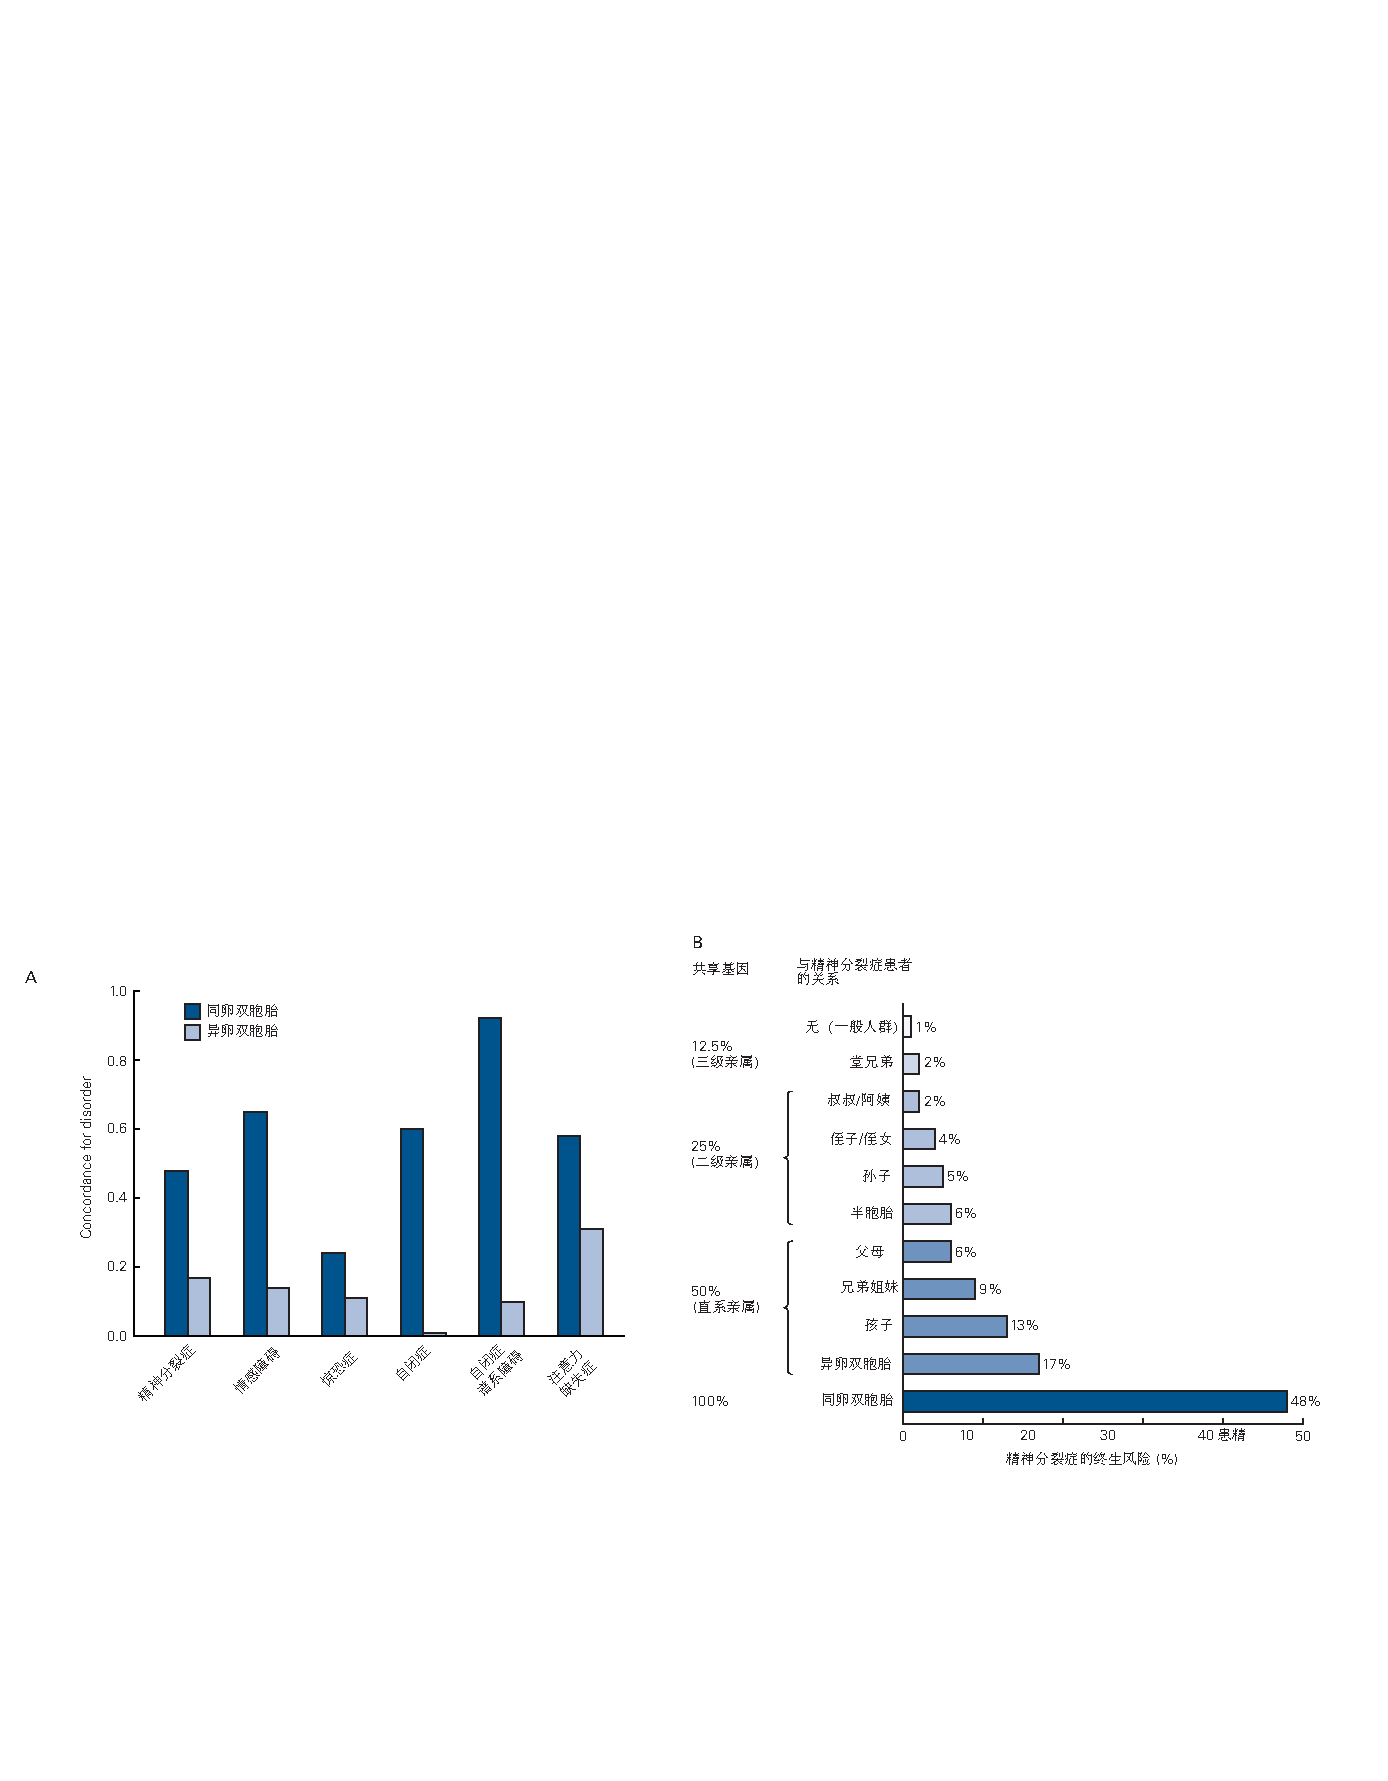
\includegraphics[width=1.0\linewidth]{chap02/fig_2_1}
	\caption{精神疾病的家族风险提供了遗传性的证据。
		\textbf{A.} 同卵双胞胎之间精神疾病的相关性比异卵双胞胎之间的相关性大得多。
		同卵双胞胎几乎共享所有基因,并且有很高(但不是 100\%)共享疾病状态的风险。
		异卵双胞胎共享 50\% 的遗传物质。
		零分表示没有相关性(两个随机人的平均结果),而 1.0 分表示完全相关\cite{mcgue1998genetic}。
		\textbf{B.} 精神分裂症患者的近亲患精神分裂症的风险更大。
		就像异卵双胞胎一样,父母和孩子以及兄弟姐妹共享 50\% 的遗传物质。
		如果只有一个基因导致精神分裂症,那么患者的父母、兄弟姐妹、孩子和异卵双胞胎的风险应该是相同的。 
		家庭成员之间的差异表明更复杂的遗传和环境因素在起作用\cite{gottesman1991schizophrenia}。}
	\label{fig:2_1}
\end{figure}


在双胞胎研究模型的一个变体中,明尼苏达双胞胎研究调查了在生命早期分开并在不同家庭中长大的同卵双胞胎。
尽管有时环境差异很大,但双胞胎对相同的精神疾病有着共同的倾向,甚至倾向于共享性格特征,比如外向性。
这项研究提供了大量证据,证明遗传变异会导致正常的人类差异,而不仅仅是疾病状态。


人类疾病和行为特征的遗传率通常大大低于 100\%,表明环境是获得疾病或特征的重要因素。
如图~\ref{fig:2_1}B~所示,来自双胞胎研究的许多神经学、精神病学和行为特征的遗传力估计值约为 50\%,但特定特征的遗传力可能更高或更低。
尽管对同卵双胞胎和其他亲属关系的研究支持人类行为具有遗传成分的观点,但它们并没有告诉我们哪些基因是重要的,更不用说特定基因如何影响行为了。
这些问题通过对实验动物的研究得到解决,其中遗传和环境因素受到严格控制,并通过现代基因发现方法得到解决,这些方法现在可以系统、可靠地识别\textit{脱氧核糖核酸}序列和结构中的特定变异,这些变异促成人类精神病学和神经学的表现型。



\section{对基因组结构和功能的理解正在演变}

分子生物学和传递遗传学的相关领域是我们现代对基因的理解的核心。
在这里,我们总结了这些领域的一些关键思想;
本章末尾的词汇表定义了常用术语。


基因由\textit{脱氧核糖核酸}组成,\textit{脱氧核糖核酸}代代相传。
在大多数情况下,每个基因的精确拷贝都会提供给生物体中的所有细胞,并通过\textit{脱氧核糖核酸}复制提供给后代。
该一般规则的罕见例外,即引入种系或体细胞\textit{脱氧核糖核酸}并在疾病风险中发挥重要作用的新(从头)突变,将在后面讨论。
\textit{脱氧核糖核酸}由两条链组成,每条链都有一个脱氧核糖磷酸骨架连接到一系列四个亚基:核苷酸\textit{腺嘌呤}、\textit{鸟嘌呤}、\textit{胸腺嘧啶}和\textit{胞嘧啶}。
如图~\ref{fig:2_2}~所示,两条链配对,一条链上的\textit{腺嘌呤}总是与互补链上的\textit{胸腺嘧啶}配对,\textit{鸟嘌呤}与\textit{胞嘧啶}配对。
这种互补性确保了\textit{脱氧核糖核酸}复制过程中\textit{脱氧核糖核酸}的准确复制,并驱动\textit{脱氧核糖核酸}转录成称为转录本的\textit{核糖核酸}长度。
鉴于几乎所有的基因组都是双链的,碱基或碱基对可以互换使用作为测量单位。
包含一千个碱基对的基因组片段称为 1 千碱基或 1 千碱基对,而一百万碱基对称为 1 兆碱基或 1 兆碱基对。
\textit{核糖核酸}与\textit{脱氧核糖核酸}的不同之处在于\textit{核糖核酸}是单链的,具有核糖而不是脱氧核糖骨架,并使用核苷碱基\textit{尿苷}代替\textit{胸腺嘧啶}。


\begin{figure}[htbp]
	\centering
	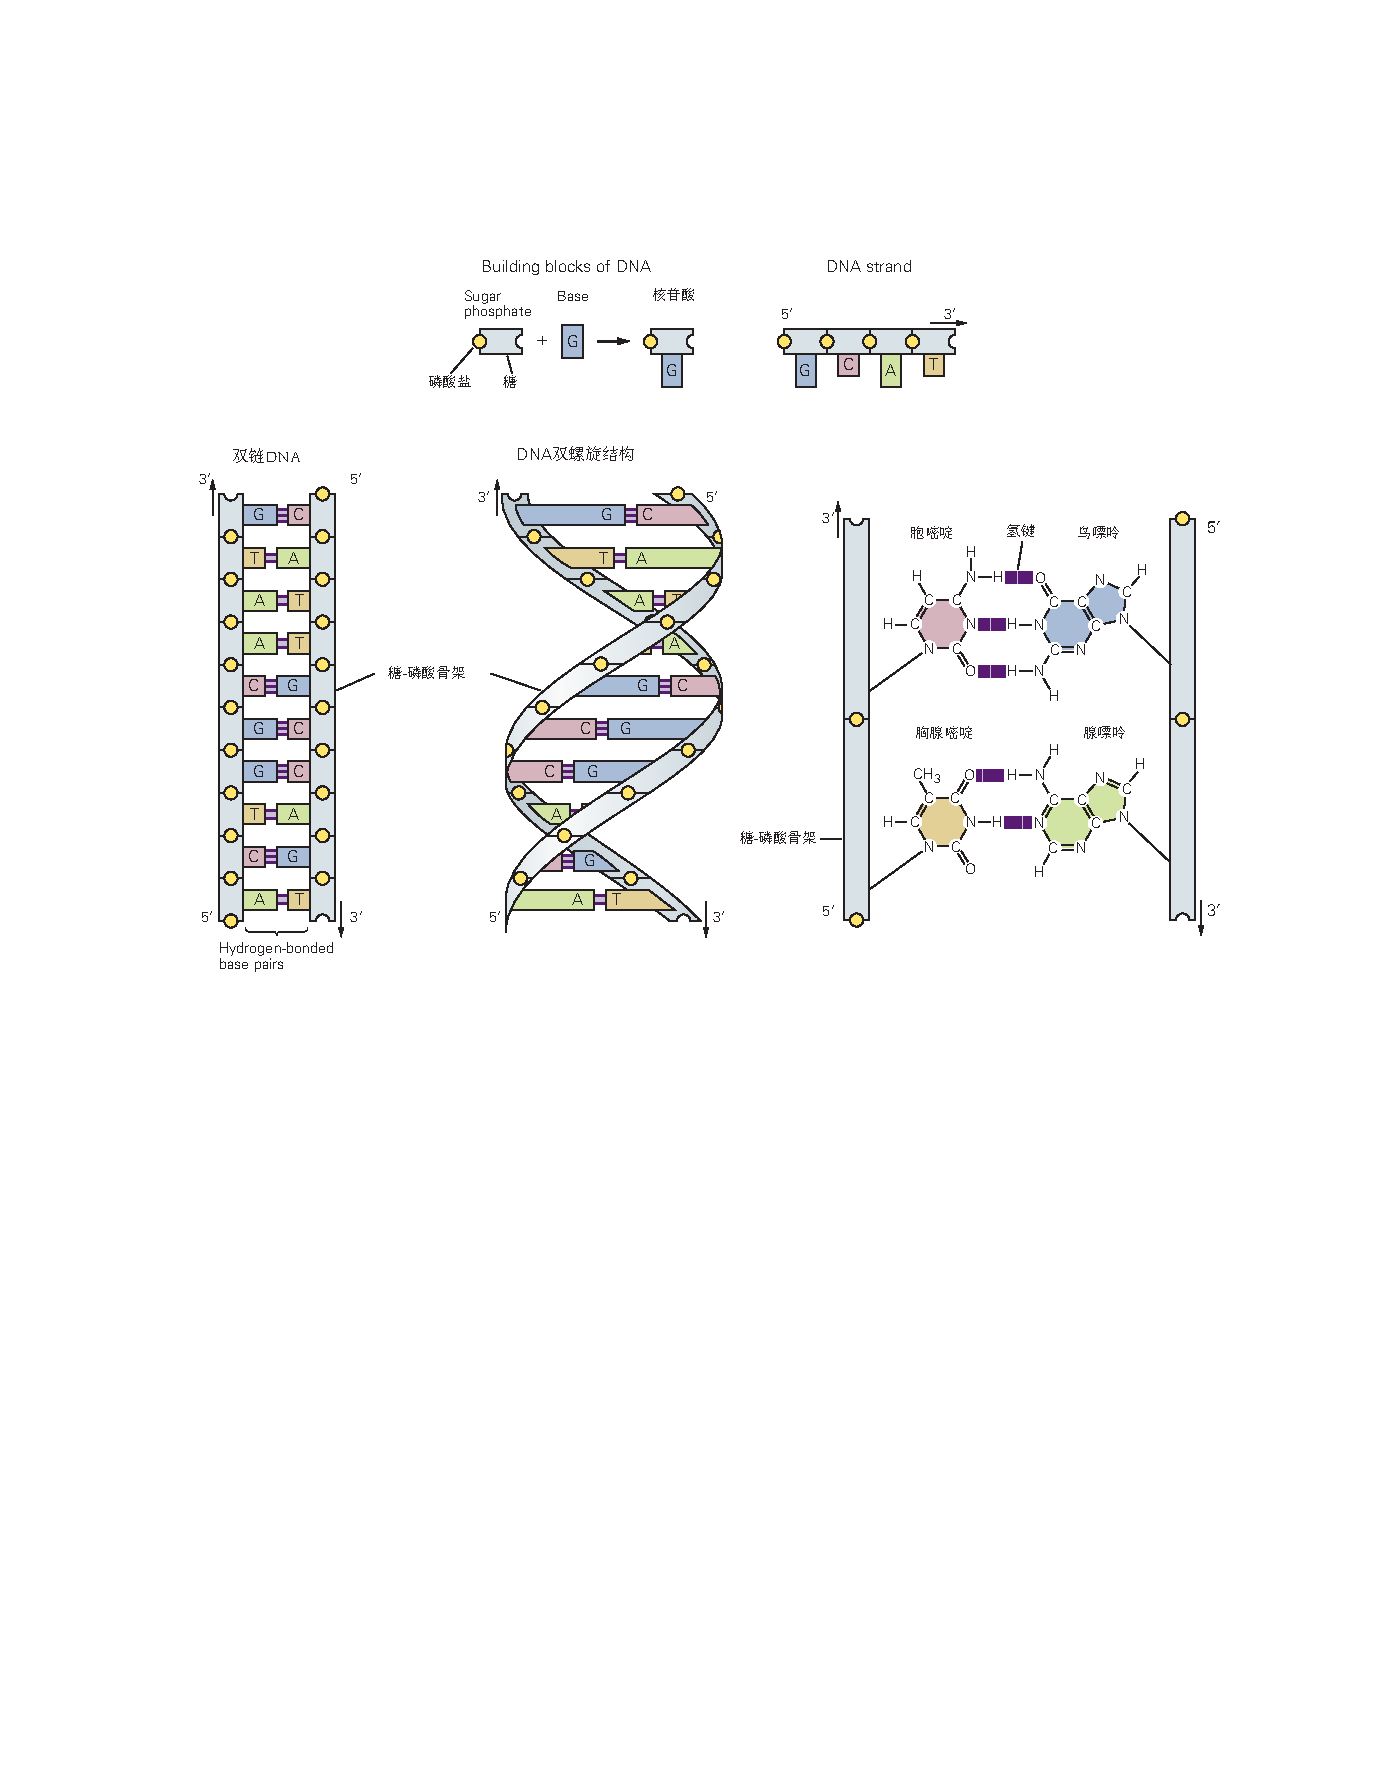
\includegraphics[width=1.0\linewidth]{chap02/fig_2_2}
	\caption{\textit{脱氧核糖核酸}的结构。
		四种不同的核苷酸碱基,腺嘌呤、胸腺嘧啶、胞嘧啶和鸟嘌呤,组装在双链\textit{脱氧核糖核酸}螺旋的糖磷酸主链上\cite{alberts2017molecular}。}
	\label{fig:2_2}
\end{figure}


在人类基因组中,大约有 2 万个基因编码蛋白质产物,这些蛋白质产物是通过将线性\textit{信使核糖核酸}序列翻译成由氨基酸组成的线性多肽(蛋白质)序列而产生的。
一个典型的蛋白质编码基因由一个编码区和非编码区组成,编码区被翻译成蛋白质(图~\ref{fig:2_3})。
编码区通常排列在称为外显子的小编码区段中,它们被称为内含子的非编码区隔开。
在翻译成蛋白质之前,内含子从\textit{信使核糖核酸}中删除。


\begin{figure}[htbp]
	\centering
	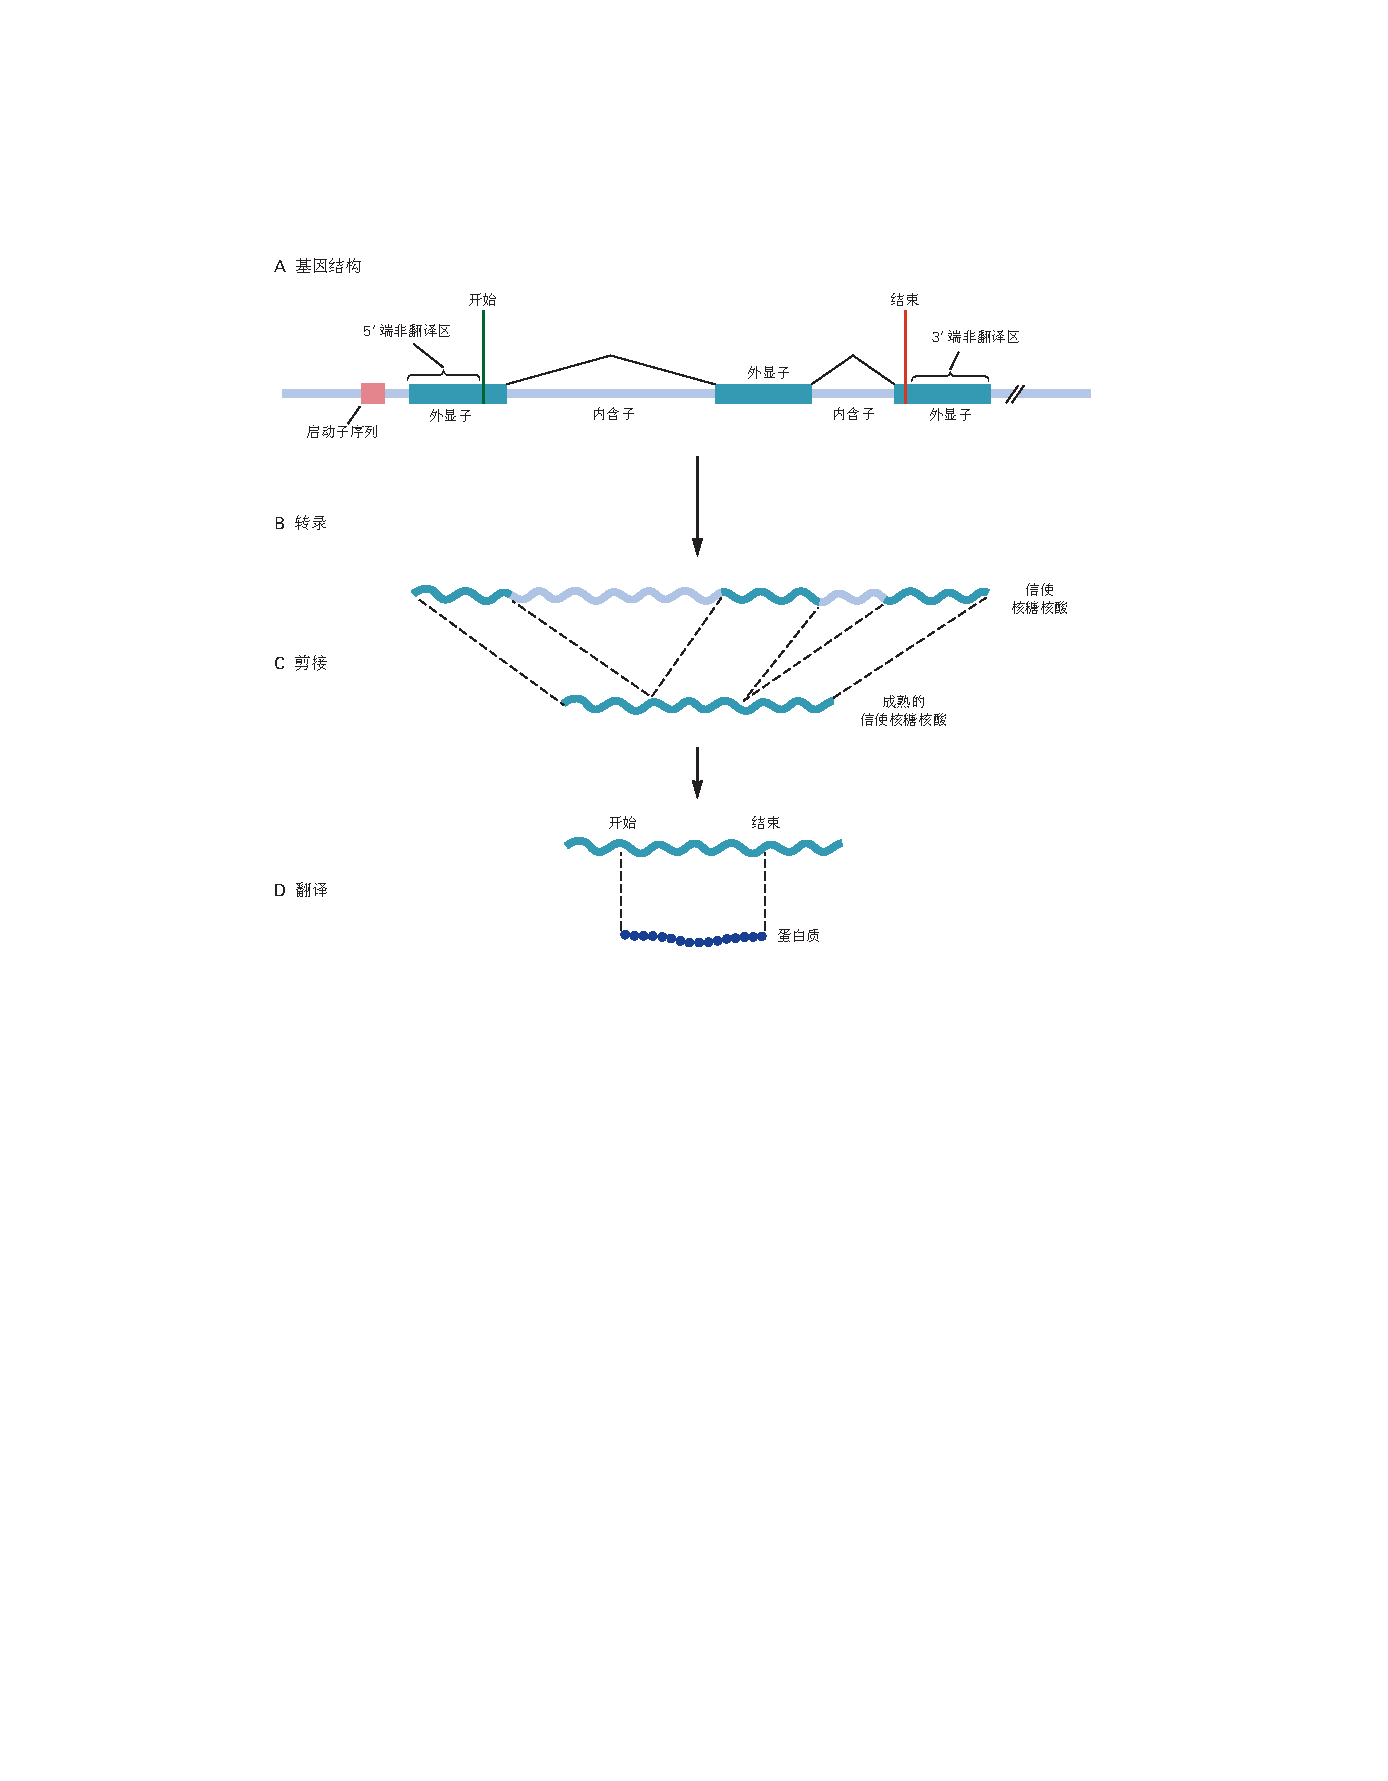
\includegraphics[width=0.96\linewidth]{chap02/fig_2_3}
	\caption{基因结构和表达。
		\textbf{A.} 一个基因由被非编码区(内含子)隔开的编码区(外显子)组成。
		它的转录受非编码区调节,例如经常在基因开始附近发现的启动子和增强子。
		\textbf{B.} 转录导致产生包括外显子和内含子的初级单链\textit{核糖核酸}转录物。
		\textbf{C.} 剪接从未成熟的转录物中去除内含子,并将外显子连接成成熟的\textit{信使核糖核酸},后者从细胞核输出。
		\textbf{D.} 成熟\textit{信使核糖核酸}的翻译产生蛋白质产物。}
	\label{fig:2_3}
\end{figure}


许多功能性\textit{核糖核酸}转录物不编码蛋白质。 
事实上,在人类基因组中,与大约 2 万个蛋白质编码基因相比,已经表征了超过 4 万个非编码转录本。
这些基因包括\textit{核糖体核糖核酸}和\textit{转运核糖核酸},它们是\textit{信使核糖核酸}翻译机制的重要组成部分。
其他\textit{非编码核糖核酸}包括\textit{长链非编码核糖核酸},任意定义为长度超过 200 \textit{碱基对},不编码蛋白质但可以在基因调控中发挥作用;
指导\textit{信使核糖核酸}剪接的多种类型的\textit{小非编码核糖核酸},包括\textit{小核核糖核酸};
和与特定\textit{信使核糖核酸}中的互补序列配对以抑制其翻译的\textit{微小核糖核酸}。


身体中的每个细胞都包含每个基因的\textit{脱氧核糖核酸},但仅将基因的特定子集表达为\textit{核糖核酸}。
转录成\textit{核糖核酸}的基因部分两侧是非编码\textit{脱氧核糖核酸}区域,这些区域可能与其他蛋白质(包括转录因子)结合以调节基因表达。
这些序列基序包括启动子、增强子、沉默子和绝缘子,它们一起允许\textit{核糖核酸}在正确的时间在正确的细胞中准确表达。
启动子通常位于待转录区域的开头附近;
增强子、消音子和绝缘子可能与被调节的基因存在一定距离。
每种类型的细胞都有独特的\textit{脱氧核糖核酸}结合蛋白补充,这些蛋白与启动子和其他调节序列相互作用,以调节基因表达和由此产生的细胞特性。


大脑表达的基因数量比身体的任何其他器官都要多,而且在大脑内,不同的神经元群表达不同的基因组。
由启动子、其他调节序列和与其相互作用的\textit{脱氧核糖核酸}结合蛋白控制的选择性基因表达允许固定数量的基因在大脑中产生数量大得多的神经元细胞类型和连接。


虽然基因指定了神经系统的初始发育和特性,但个体的经历和特定神经回路中由此产生的活动本身可以改变基因的表达。
通过这种方式,环境影响被纳入神经回路的结构和功能。
基因研究的一些主要目标是阐明单个基因影响生物过程的方式、基因网络影响彼此活动的方式以及基因与环境相互作用的方式。



\subsection{基因排列在染色体上}

细胞中的基因有序地排列在称为染色体的长而线性的\textit{脱氧核糖核酸}上。
人类基因组中的每个基因都可重复地位于特定染色体上的特征位置(\textit{基因座}),并且该遗传“地址”可用于将生物学特征与基因的作用相关联。
大多数多细胞动物(包括蠕虫、果蝇和小鼠,以及人类)都是二倍体;
每个体细胞都携带两套完整的染色体,一套来自母亲,另一套来自父亲。


人类有大约 2 万个基因,但只有 46 条染色体:
22 对常染色体(男性和女性都存在的染色体)和两条性染色体(女性有两条 X 染色体,男性有一条 X 染色体和一条 Y 染色体)(图~\ref{fig:2_4})。
每个父母都向二倍体后代提供每个常染色体的一个副本。
每个父母也为女性(XX)后代提供一条 X 染色体,但 XY 男性从母亲那里继承了一条 X 染色体,从父亲那里继承了一条 Y 染色体。
1910 年,\textit{摩尔根}在果蝇身上发现了\textit{伴性遗传}。
这种与单个 X 染色体相关的\textit{伴性遗传}模式在人类遗传学研究中非常重要,某些 X 连锁遗传病通常仅在男性,但基因会从母亲传给儿子。


\begin{figure}[htbp]
	\centering
	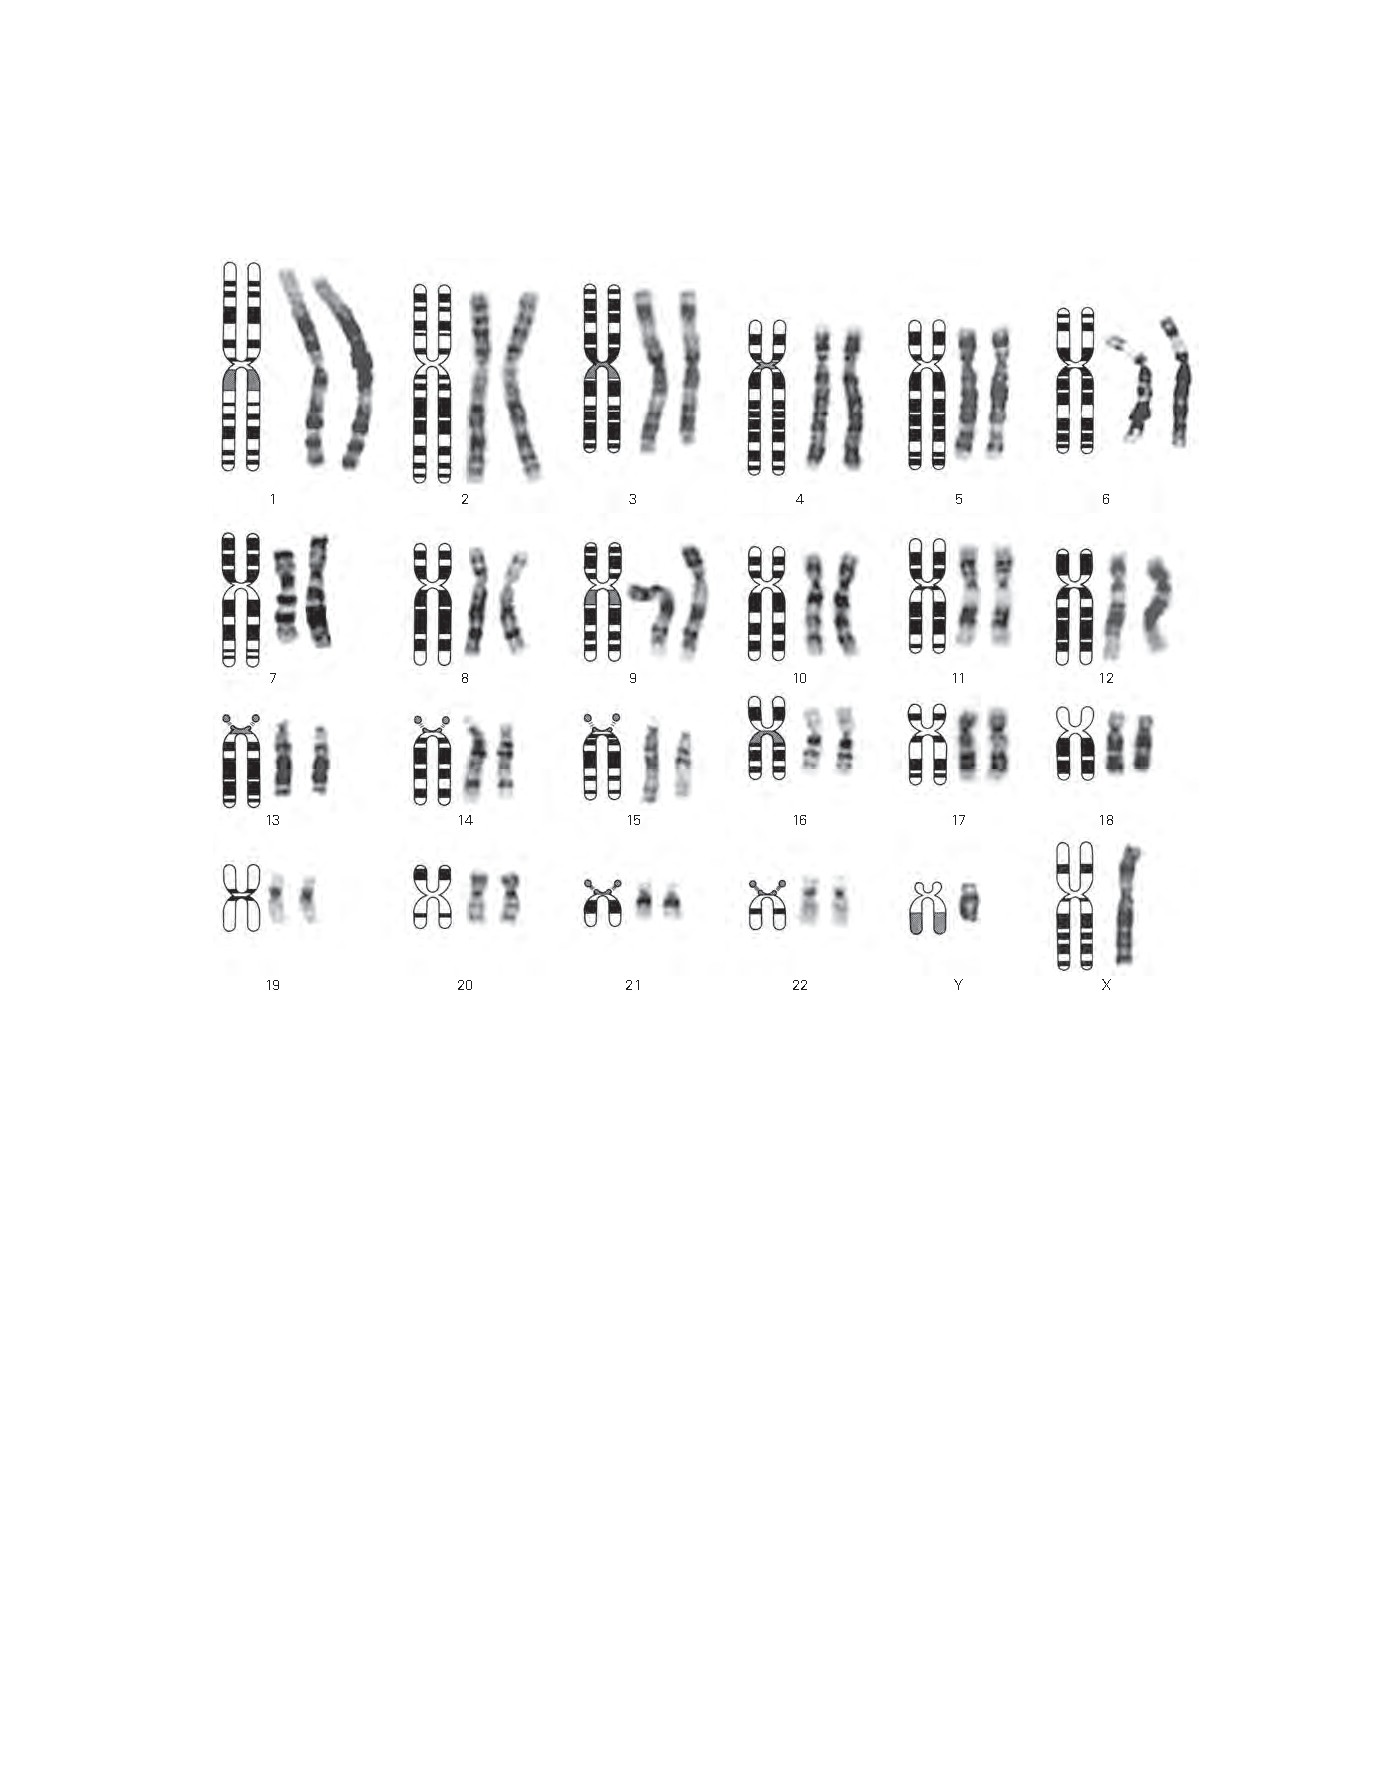
\includegraphics[width=0.95\linewidth]{chap02/fig_2_4}
	\caption{中期正常人类染色体的图解说明了每条染色体的独特形态。
		特征大小和特征亮区和暗区允许染色体彼此区分\cite{watoson1983recombinant}。}
	\label{fig:2_4}
\end{figure}


除了染色体上的基因外,极少数生物体基因通过线粒体传递,线粒体是执行代谢过程的细胞质细胞器。
所有儿童的线粒体都来自卵子,因此会从母亲传给孩子。
某些人类疾病,包括某些神经肌肉退行性疾病、某些形式的智力障碍和某些形式的耳聋,都是由线粒体\textit{脱氧核糖核酸}突变引起的。



\section{基因型和表现型之间的关系通常很复杂}

个体中特定常染色体基因的两个拷贝称为\textit{等位基因}。
如果两个\textit{等位基因}相同,则称个体在该位点是纯合的。
如果等位基因因突变而不同,则个体在该位点是杂合的。
男性是 X 染色体上基因的半合子。
一个群体可以有一个基因的大量等位基因;
例如,影响人眼颜色的单个\textit{2 型眼皮肤白化病}基因可以具有编码蓝色、绿色、淡褐色或棕色色调的等位基因。
由于这种变异,区分生物体的基因型(其基因组成)和表型(其外观)非常重要。
从广义上讲,基因型是构成个体基因组的整套等位基因;
狭义上,就是一个基因的特异等位基因。
相比之下,表型是对整个生物体的描述,是生物体基因型在特定环境中表达的结果。


如果突变表型仅在基因的两个等位基因都发生突变时才表达,则产生的表型称为隐性。
如果个体是突变等位基因的纯合子,或者如果他们在每个染色体上的给定基因中携带不同的破坏性等位基因(所谓的复合杂合子),就会发生这种情况。
隐性突变通常是由功能蛋白的丢失或减少引起的。
在人类和实验动物中普遍观察到突变性状的隐性遗传。


如果突变表型由一个突变体和一个野生型等位基因的组合产生,则表型特征和突变等位基因被认为是显性的。
一些突变是显性的,因为 50\% 的基因产物不足以形成正常表型(单倍体不足)。
其他显性突变导致异常蛋白质的产生或野生型基因产物在不适当的时间或地点的表达;
如果这对正常的蛋白质产物起拮抗作用,则称为显性失活突变。


当考虑具有同一基因的一个正常(野生型)等位基因和一个突变等位基因的后果时,基因型和表型之间的差异是显而易见的。
一系列神经发育障碍(包括孤独症和癫痫)的基因发现的最新进展表明,人类基因组对单倍体不足比以前认为的更敏感。
然而,虽然一个基因的两个拷贝的完全失活通常具有可靠的效果,但单倍体不足的严重性和表现在个体之间差异更大,这种现象称为可变、部分或不完全外显率。


干扰人类发育、细胞功能或行为的遗传变异落在共同等位基因(也称为多态性)和稀有变异之间的连续体上,前者通常对生物学和行为具有较小的个体影响,后者可能具有较大的生物学效应(方框~\ref{box:2_1})。
虽然这些分类是有用的概括,但在一些重要的案例中,常见的多态性会带来很大的疾病风险;
\textit{载脂蛋白E}基因的一种常见变异,存在于 16\% 的人口中,导致迟发性阿尔茨海默病的风险增加四倍。


\begin{proposition}[突变:遗传多样性的起源] \label{box:2_1}
	
	\quad \quad 尽管\textit{脱氧核糖核酸}复制通常是以高保真度进行的,但被称为突变的自发错误确实会发生。
	突变可能是由\textit{脱氧核糖核酸}中嘌呤和嘧啶碱基的损伤、\textit{脱氧核糖核酸}复制过程中的错误以及减数分裂过程中发生的重组引起的。
	
	
	\quad \quad 编码区内单个\textit{脱氧核糖核酸}碱基(也称为点突变)的变化分为五大类:
	
	
	1. 无声突变会改变碱基,但不会导致编码蛋白质发生明显变化。
	
	
	2. \textit{错义突变}是一种点突变,导致蛋白质中的一个氨基酸被另一个氨基酸取代;
	利用信息学和经验证据,这些突变被越来越多地分为至少两个亚类:损害蛋白质功能的突变和功能中性的突变。
	
	
	3. \textit{无义突变}是指其中指定特定氨基酸的编码区内的密码子(三重核苷酸)被终止密码子取代,导致蛋白质产物缩短(截短)。
	
	
	4. \textit{经典剪切位点突变}改变了指定外显子/内含子边界的核苷酸。
	
	5. \textit{框移突变}是指其中核苷酸的小片段插入或缺失改变了阅读框架,导致产生截短或异常的蛋白质。
	
	\quad \quad 在目前的文献中,属于后四类的突变(包括破坏性错义突变)通常被称为\textit{可能的基因破坏}突变。
	
	\quad \quad 在实验遗传学研究中,当生物体暴露于化学诱变剂或电离辐射时,突变的频率会大大增加。
	化学诱变剂倾向于诱导\textit{点突变},涉及单个\textit{脱氧核糖核酸}碱基对的变化或几个碱基对的缺失。
	电离辐射可诱导大量插入、缺失或易位。
	
	\quad \quad 在人类中,\textit{点突变}在\textit{卵母细胞}和精子中以较低的自发率发生,导致孩子出现突变,但父母双方都没有,称为\textit{新生突变}。
	每一代,整个基因组(约30亿个碱基对)都会发生70至90个单碱基变化,其中一个碱基对平均会导致蛋白质编码基因的\textit{错义突变}或\textit{无义突变}。
	父亲年龄较大的孩子新发点突变的数量增加,而母亲年龄较大的儿童染色体异常的频率增加。
	
	
	\quad \quad 随着2001年人类基因组测序和检测基因变异的高分辨率方法的不断提高,现在也很清楚,点突变并不是人类之间唯一的序列差异。
	某些序列可能在染色体上缺失或重复多次,因此在不同的个体中可能具有不同数量的拷贝。
	超过一个碱基和少于1000个碱基对的变化被称为\textit{插入缺失突变}。
	当这种变异包含超过1000个碱基对时,它们被称为\textit{拷贝数变异}。
	
	
	\quad \quad 任何基因变异对疾病或综合症的贡献都可以被称为简单的(或孟德尔的)或复杂的。
	一般来说,一个简单的或孟德尔突变是一个足以赋予表型而没有额外遗传风险的突变。
	这并不意味着每个有突变的人都会表现出完全相同的表型。
	然而,特定疾病等位基因和表型之间通常存在高度可靠的关系,这种关系接近一对一的关系(如镰状细胞性贫血或亨廷顿舞蹈症)。
	
	
	\quad \quad 相反,复杂的遗传疾病是指遗传风险因素改变了疾病的概率,但并不是完全的因果关系。
	这种遗传贡献可能涉及罕见的突变、常见的多态性或两者兼有,并且通常是非常异质的,多个不同的基因和等位基因具有增加风险或发挥保护作用的能力。
	大多数复杂的疾病也与环境有关。
	
		
\end{proposition}



\section{基因在进化中得以保存}

2001年报道了人类基因组近乎完整的核苷酸序列,许多动物基因组的完整核苷酸序列也已被破译。
这些基因组之间的比较得出了一个令人惊讶的结论:
独特的人类物种并非源于独特的新人类基因发明。


人类和黑猩猩在生物学和行为上有很大不同,但它们 99\% 的蛋白质编码基因是相同的。
此外,人类大约 2 万个基因中的大部分也存在于其他哺乳动物(例如小鼠)中,并且超过一半的人类基因与无脊椎动物(例如蠕虫和苍蝇)中的基因非常相似(图~\ref{fig:2_5})。
这一令人惊讶的发现得出的结论是,人类与其他动物共有的古老基因以新的方式受到调节,从而产生新的人类特性,例如产生复杂思想和语言的能力。


\begin{figure}[htbp]
	\centering
	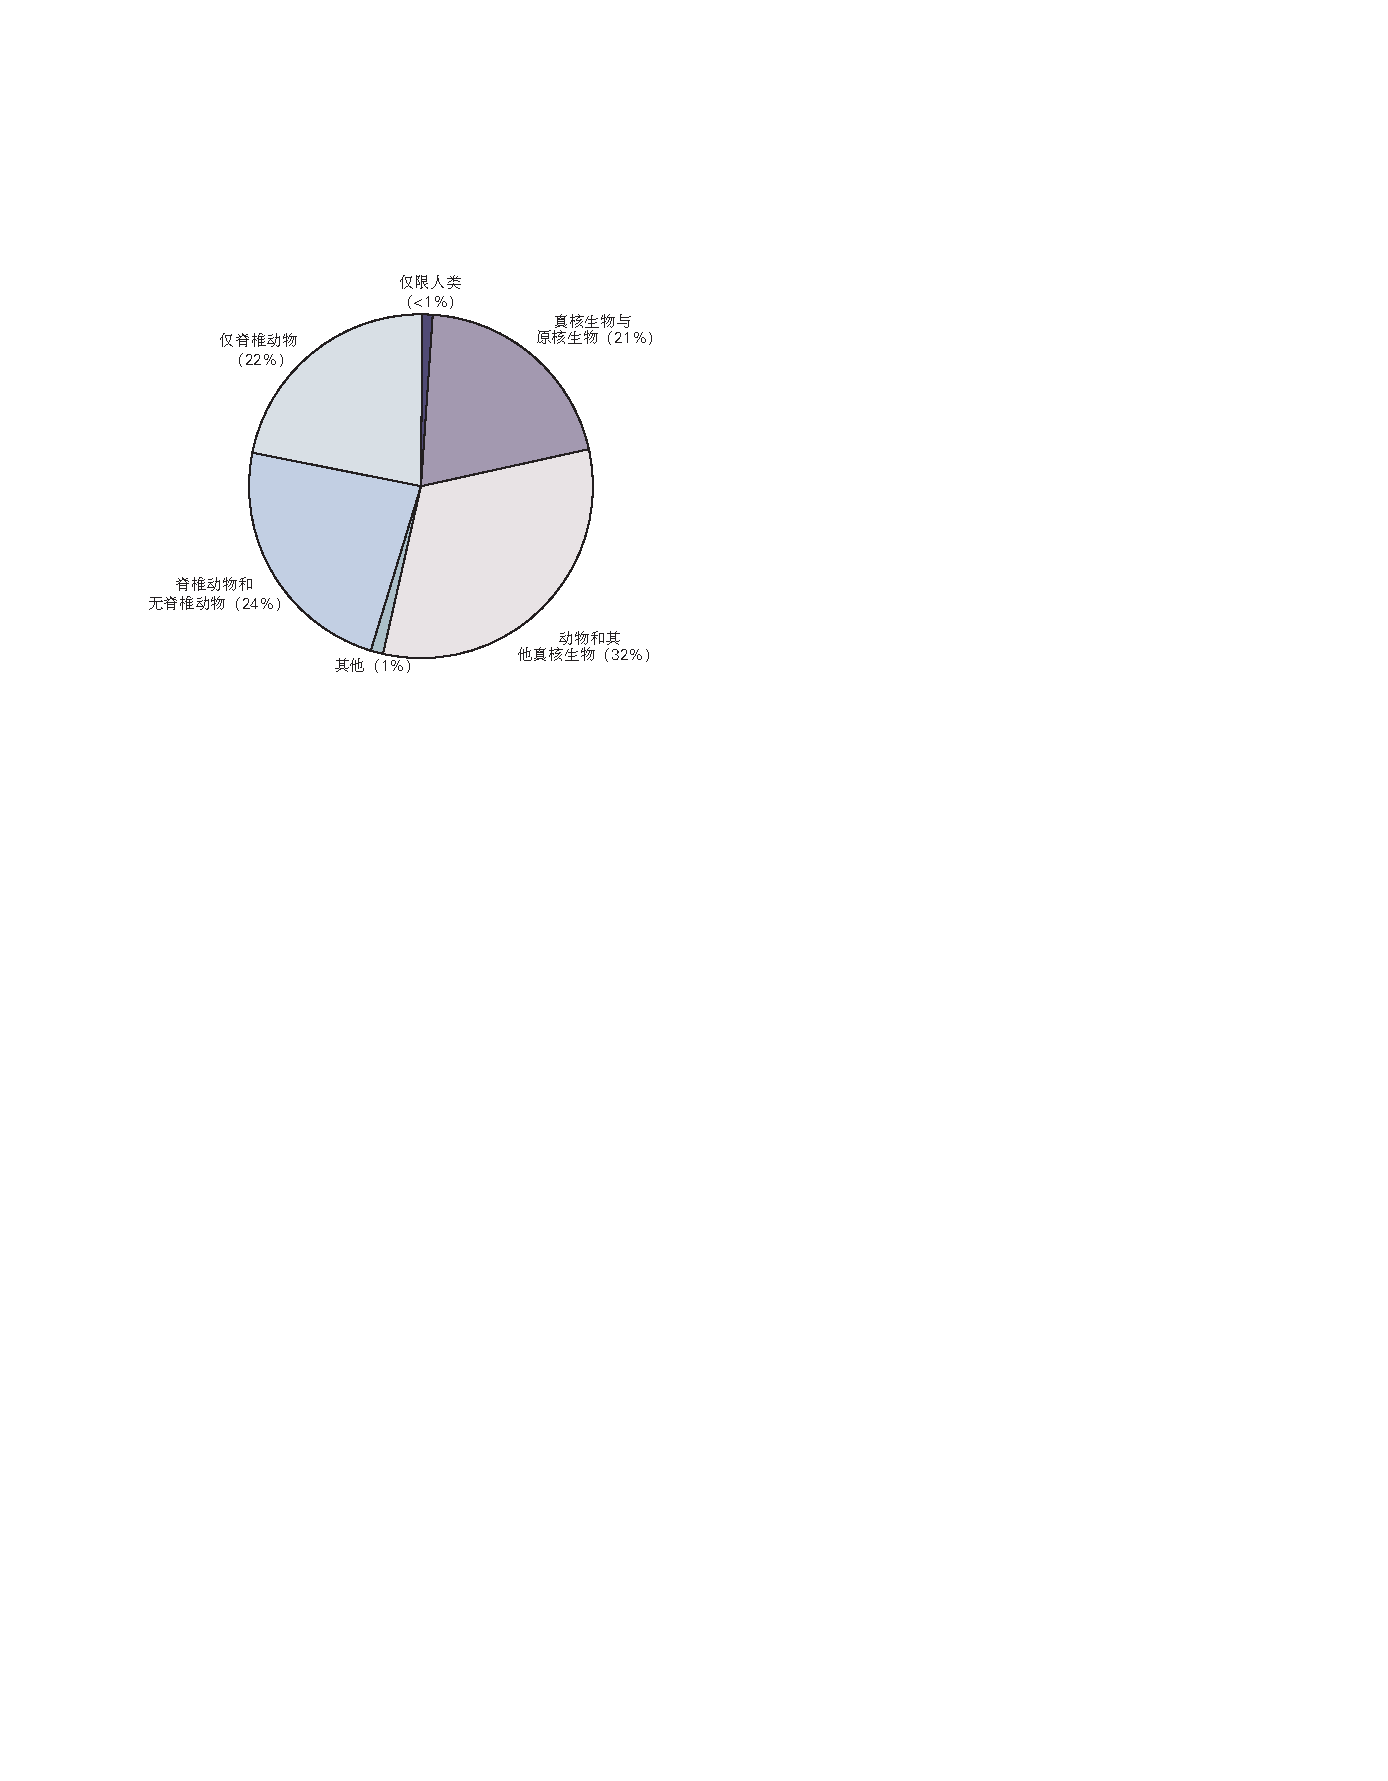
\includegraphics[width=0.6\linewidth]{chap02/fig_2_5}
	\caption{大多数人类基因都与其他物种的基因有关。
		不到 1\% 的人类基因是人类特有的;其他基因可能为所有生物、所有真核生物、仅动物或仅脊椎动物共享\cite{international2001initial}。}
	\label{fig:2_5}
\end{figure}


由于在整个进化过程中基因的这种保守性,对一种动物的研究的见解通常可以应用于具有相关基因的其他动物,这是一个重要的事实,因为动物实验通常是可能的,而人类实验却不可能。
例如,编码与人类基因相似的氨基酸序列的小鼠基因通常具有与直向同源人类基因相似的功能。


大约一半的人类基因具有已从其他生物体的直系同源基因中证明或推断出的功能(图~\ref{fig:2_6})。
人类、苍蝇甚至单细胞酵母共有的一组基因编码用于中间代谢的蛋白质;
\textit{脱氧核糖核酸}、\textit{核糖核酸}和蛋白质的合成;
细胞分裂; 和细胞骨架结构、蛋白质运输和分泌。


\begin{figure}[htbp]
	\centering
	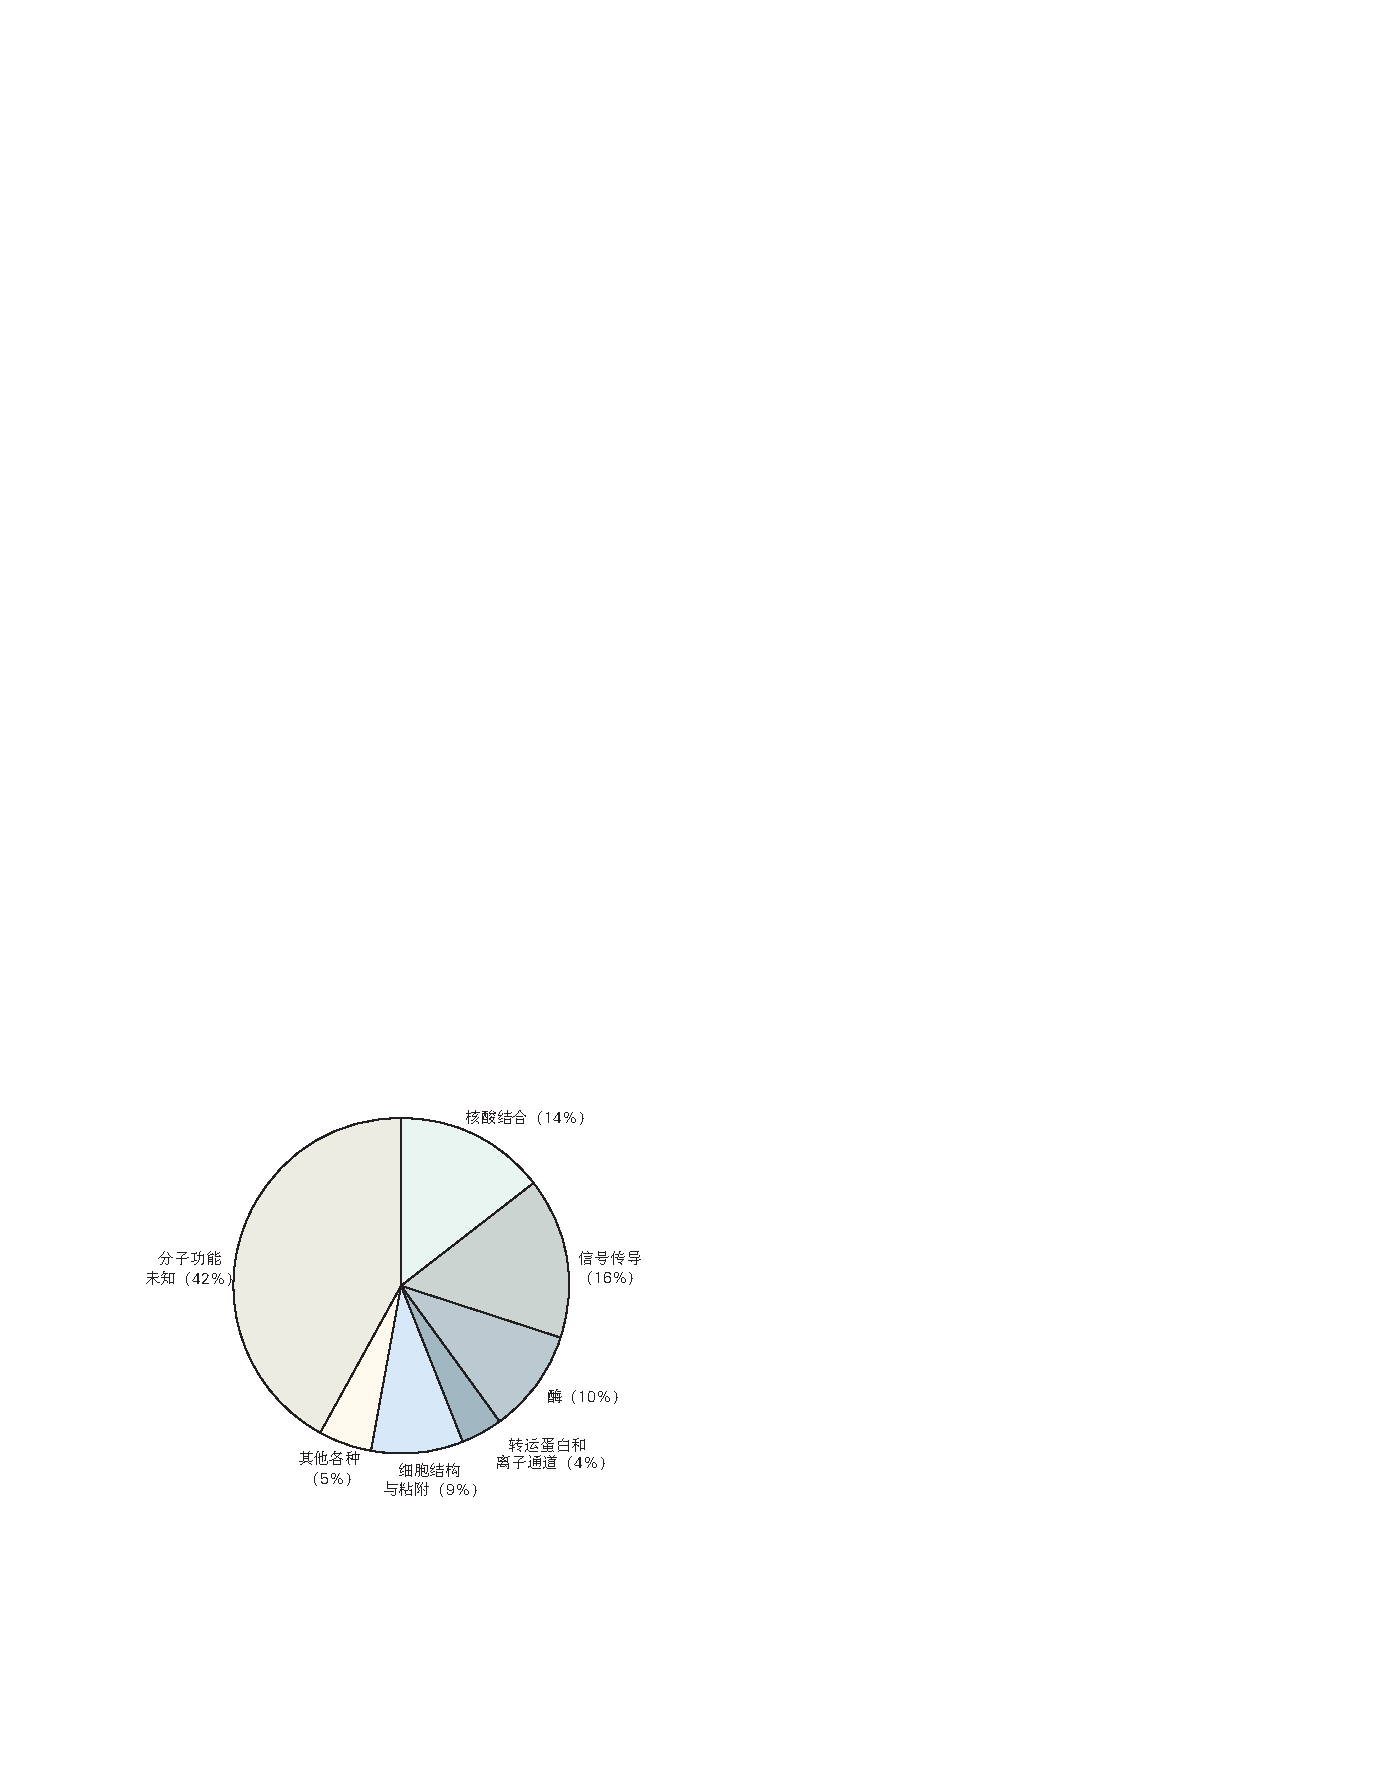
\includegraphics[width=0.6\linewidth]{chap02/fig_2_6}
	\caption{26,383 个人类基因的预测分子功能\cite{venter2001sequence}。}
	\label{fig:2_6}
\end{figure}


从单细胞生物到多细胞动物的进化伴随着与细胞间信号传导和基因调控有关的基因的扩展。
多细胞动物(例如蠕虫、苍蝇、小鼠和人类)的基因组通常编码数千个跨膜受体,比单细胞生物中存在的多得多。 
这些跨膜受体用于发育过程中的细胞间通讯、神经元之间的信号传递以及作为环境刺激的传感器。
多细胞动物的基因组还编码 1 千种或更多不同的\textit{脱氧核糖核酸}结合蛋白,这些蛋白调节其他基因的表达。


人类的许多跨膜受体和\textit{脱氧核糖核酸}结合蛋白与其他脊椎动物和无脊椎动物的特定直系同源基因相关。
通过列举动物共有的遗传基因,我们可以推断出神经元发育、神经传递、电兴奋性和基因表达的基本分子通路存在于蠕虫、苍蝇、小鼠和人类的共同祖先中。
此外,对动物和人类基因的研究表明,人脑中最重要的基因是那些在整个动物系统发育过程中最保守的基因。
哺乳动物基因与其无脊椎动物基因之间的差异通常是由哺乳动物基因复制或基因表达和功能的细微变化引起的,而不是全新基因的产生。



\section{可以在动物模型中研究行为的遗传调控}

由于人类和动物基因之间的进化保守性,在动物模型中研究构成行为基础的基因、蛋白质和神经回路之间的关系可能会深入了解人类的这些关系。
在基因功能研究中应用了两个重要策略并取得了巨大成功。


在经典的遗传分析中,生物体首先受到化学诱变或辐射诱导随机突变,然后筛选影响感兴趣行为(例如睡眠)的可遗传变化。
这种方法不会对所涉及的基因类型施加偏见;
它是对所有可能导致可检测到的变化的突变的随机搜索。 
可遗传变化的遗传追踪允许识别突变生物体中改变的个体基因。
因此,经典遗传学的发现路径从表型到基因型,从生物体到基因。
在反向遗传学中,特定的感兴趣基因被作为改变的目标,产生转基因动物,并研究具有这些改变基因的动物。
这种策略既有重点又有偏见:一个是从特定基因开始,发现的途径是从基因型到表型,从基因到生物体。


这两种实验策略及其更微妙的变化构成了实验遗传学的基础。
经典和反向遗传学的基因操作是在实验动物身上进行的,而不是在人类身上。



\subsection{转录振荡器调节苍蝇、小鼠和人类的昼夜节律}

\textit{西摩$\cdot$本泽}和他的同事在 1970 年左右发起了关于基因对行为影响的第一次大规模研究。
他们使用随机诱变和经典遗传分析来识别影响\textit{黑腹果蝇}习得和先天行为的突变:
昼夜节律(每天)节奏、求爱行为、运动、视觉感知和记忆(方框~\ref{box:2_2}~和方框~\ref{box:2_3})。
这些诱导突变对我们理解基因在行为中的作用产生了巨大影响。


\begin{proposition}[在实验动物中产生突变] \label{box:2_2}
	
	\quad \quad 苍蝇的随机诱变
	
	\quad \quad \textit{果蝇}行为的遗传分析是在个体基因发生突变的果蝇身上进行的。
	突变可以通过化学诱变或插入诱变进行,这些策略可以影响基因组中的任何基因。
	类似的随机诱变策略被用于在线虫\textit{秀丽隐杆线虫}、斑马鱼和小鼠中产生突变。
	
	\quad \quad 化学诱变,例如用\textit{甲磺酸乙酯},通常会在基因中产生随机点突变。
	当被称为转座子的可移动\textit{脱氧核糖核酸}序列随机插入其他基因时,就会发生插入突变。
	
	\quad \quad 果蝇中最广泛使用的转座元件是P元件。
	P元件可以被修饰为携带眼睛颜色的遗传标记,这使得它们在遗传杂交中易于追踪,并且它们也可以被修饰以改变它们所插入的基因的表达。
	
	\quad \quad 为了引起P元件转位,携带P元件的果蝇菌株被杂交到不携带的果蝇菌株。
	这种遗传杂交会导致所产生的后代中P元件的不稳定和移位。
	P元件的动员导致其在随机基因中转移到新的位置。
	
	\quad \quad 小鼠的靶向诱变
	
	\quad \quad 哺乳动物基因分子操作的进展已经允许用突变版本精确替换已知的正常基因。
	产生突变小鼠菌株的过程涉及两种不同的操作。
	染色体上的基因被称为胚胎干细胞的特殊细胞系中的同源重组所取代,修饰后的细胞系被整合到胚胎的生殖细胞群中(图~\ref{fig:2_7}f)。
	
	\quad \quad 必须首先克隆感兴趣的基因。
	该基因发生突变,然后将选择性标记(通常是耐药性基因)引入突变片段中。
	然后将改变的基因引入胚胎干细胞,并分离出包含改变基因的细胞克隆。
	对每个克隆的\textit{脱氧核糖核酸}样本进行测试,以鉴定突变基因已整合到同源(正常)位点而不是其他一些随机位点的克隆。
	
	\quad \quad 当已经鉴定出合适的克隆时,在胚泡阶段(受精后3至4天)将细胞注射到小鼠胚胎中,此时胚胎由大约100个细胞组成。
	然后,这些胚胎被重新引入一只雌性体内,这只雌性已经为植入做了激素准备,并被允许足月。
	得到的胚胎是干细胞系和宿主胚胎之间的嵌合混合物。
	
	\quad \quad 小鼠的胚胎干细胞有能力参与发育的各个方面,包括生殖系。
	注射的细胞可以成为生殖细胞,并将改变后的基因传递给后代小鼠。
	这项技术已被用于在对神经系统发育或功能至关重要的各种基因中产生突变。
	
	\quad \quad 限制基因敲除和调控转基因表达
	
	\quad \quad 为了提高基因敲除技术的实用性,已经开发出将缺失限制在特定组织中或动物发育过程中特定点的细胞上的方法。
	区域限制的一种方法利用Cre/loxP系统。
	Cre/loxP系统是来源于P1噬菌体的位点特异性重组系统,其中噬菌体酶Cre重组酶催化34bp loxP识别序列之间的重组,这些序列通常不存在于动物基因组中。
	
	\quad \quad loxP序列可以通过同源重组插入胚胎干细胞的基因组中,使得它们位于感兴趣基因(称为floxed基因)的一个或多个外显子的侧翼。
	当干细胞被注射到胚胎中时,人们最终可以培育出一只小鼠,其中感兴趣的基因是游离的,并且仍然在动物的所有细胞中发挥作用。
	
	\quad \quad 然后可以产生第二批转基因小鼠,其在神经启动子序列的控制下表达Cre重组酶,该序列通常在受限的大脑区域中表达。
	通过将Cre转基因小鼠系与具有感兴趣的游离基因的小鼠系杂交,该基因将仅在表达Cre转基因的那些细胞中被删除。
	
	\quad \quad 在图~\ref{fig:2_8}A所示的例子中,编码\textit{N-甲基-D-天冬氨酸}谷氨酸受体NR1(或GluN1)亚基的基因被loxP元件侧翼,然后在\textit{钙/钙调蛋白依赖性蛋白激酶 2}启动子的控制下与表达Cre重组酶的小鼠系杂交,该启动子通常在前脑神经元中表达。
	在这个特定的细胞系中,表达偶然局限于海马\textit{阿蒙角}1区,导致该脑区NR1亚基的选择性缺失(图~\ref{fig:2_8}B)。
	因为\textit{钙/钙调蛋白依赖性蛋白激酶 2}启动子只在出生后激活基因转录,所以这种策略可以最大限度地减少早期发育变化。
	
	\quad \quad 除了基因表达的区域限制外,对基因表达时间的控制给研究者提供了额外的灵活性,并可以排除在成熟动物表型中观察到的任何异常是转基因产生的发育缺陷的结果的可能性。
	这可以在小鼠身上通过构建一种可以用药物开启或关闭的基因来实现。
	
	\quad \quad 一个是从创建两个小鼠行开始。
	品系1携带一种特殊的转基因,该转基因受启动子\textit{四环素反应元件}的控制,而\textit{四环素反应元件}通常只在细菌中发现。
	这个启动子本身不能启动基因;它需要被特定的转录调节因子激活。
	因此,第二组小鼠表达第二种转基因,该转基因编码一种杂交转录因子\textit{四环素激活因子},该因子识别并结合\textit{四环素反应元件}启动子。
	\textit{四环素激活因子}的表达可以置于小鼠基因组中的启动子的控制下,该启动子通常仅在特定类别的神经元或特定大脑区域中驱动基因转录。
	
	\quad \quad 当这两种小鼠交配时,一些后代将携带两种转基因。
	在这些小鼠中,\textit{四环素激活因子}与\textit{四环素反应元件}启动子结合并激活下游转基因。
	\textit{四环素激活因子}转录因子之所以特别有用,是因为当它与某些抗生素(如四环素)结合时,它会失活,从而通过给小鼠服用抗生素来调节转基因表达。
	还可以产生表达被称为反向\textit{四环素激活因子}的\textit{四环素激活因子}突变形式的小鼠。
	这种反式激活剂不会与\textit{四环素反应元件}结合,除非动物被喂食多西环素。
	在这种情况下,转基因总是被关闭,除非给药(图~\ref{fig:2_9})。
	
	\quad \quad \textit{核糖核酸}干扰和\textit{规律成簇的间隔短回文重复}改变基因功能
	
	\quad \quad 最后,可以通过现代分子工具靶向基因来灭活基因。
	一种这样的方法是\textit{核糖核酸}干扰,它利用了真核细胞中大多数双链\textit{核糖核酸}被常规破坏的事实;即使只有一部分是双链的,整个\textit{核糖核酸}也会被破坏。
	通过引入一个短\textit{核糖核酸}序列,人工地使选定的\textit{信使核糖核酸}变成双链,研究人员可以激活这一过程,降低特定基因的\textit{信使核糖核酸}水平。
	
\end{proposition}


\begin{figure}[htbp]
	\centering
	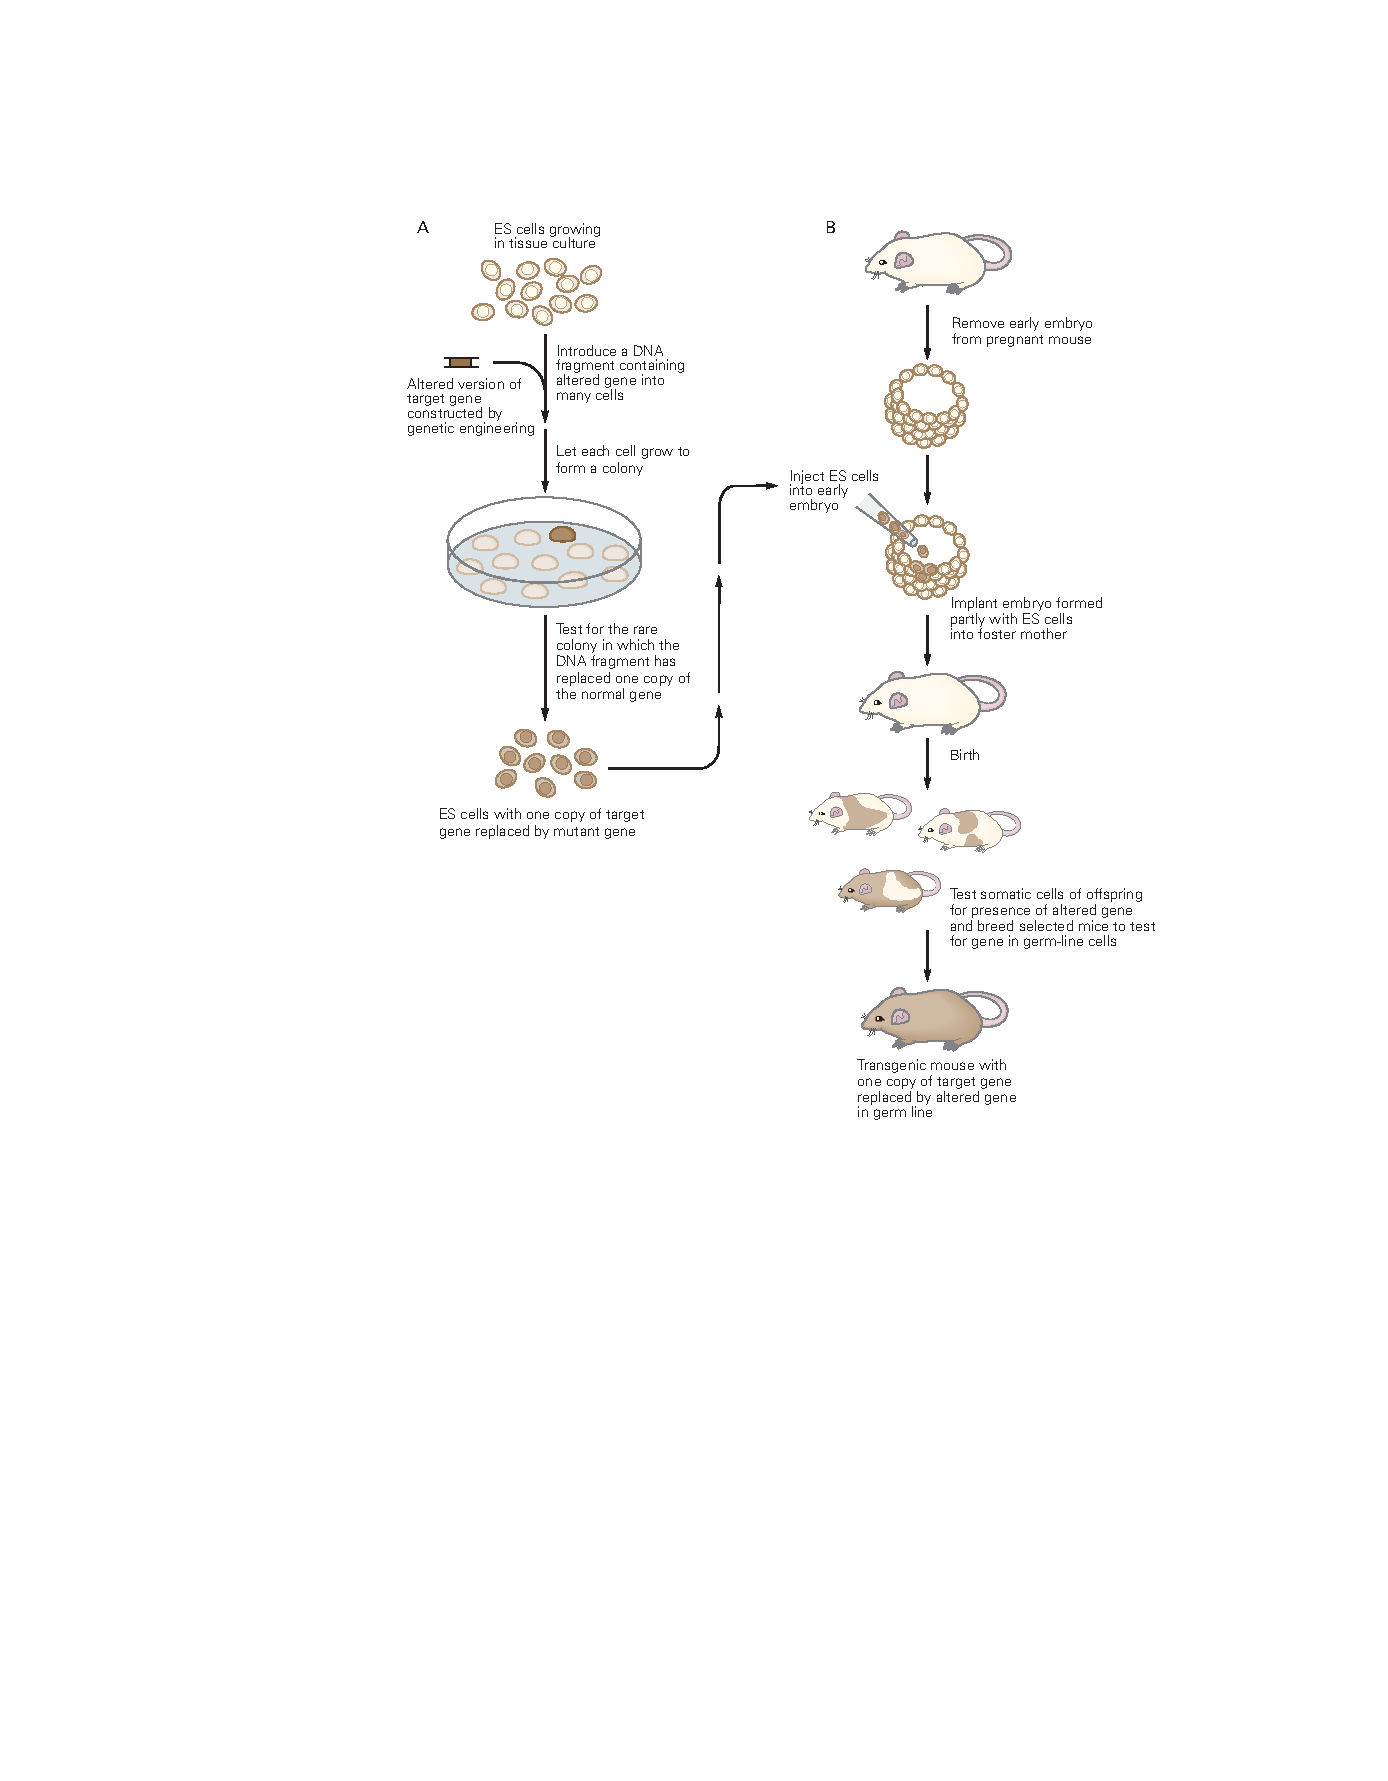
\includegraphics[width=0.94\linewidth]{chap02/fig_2_7}
	\caption{创造突变小鼠菌株\cite{alberts2017molecular}。
		\textbf{A.} 产生具有特定靶向突变的小鼠干细胞。
		\textbf{B.} 利用改变的胚胎干细胞创造转基因小鼠。}
	\label{fig:2_7}
\end{figure}


\begin{figure}[htbp]
	\centering
	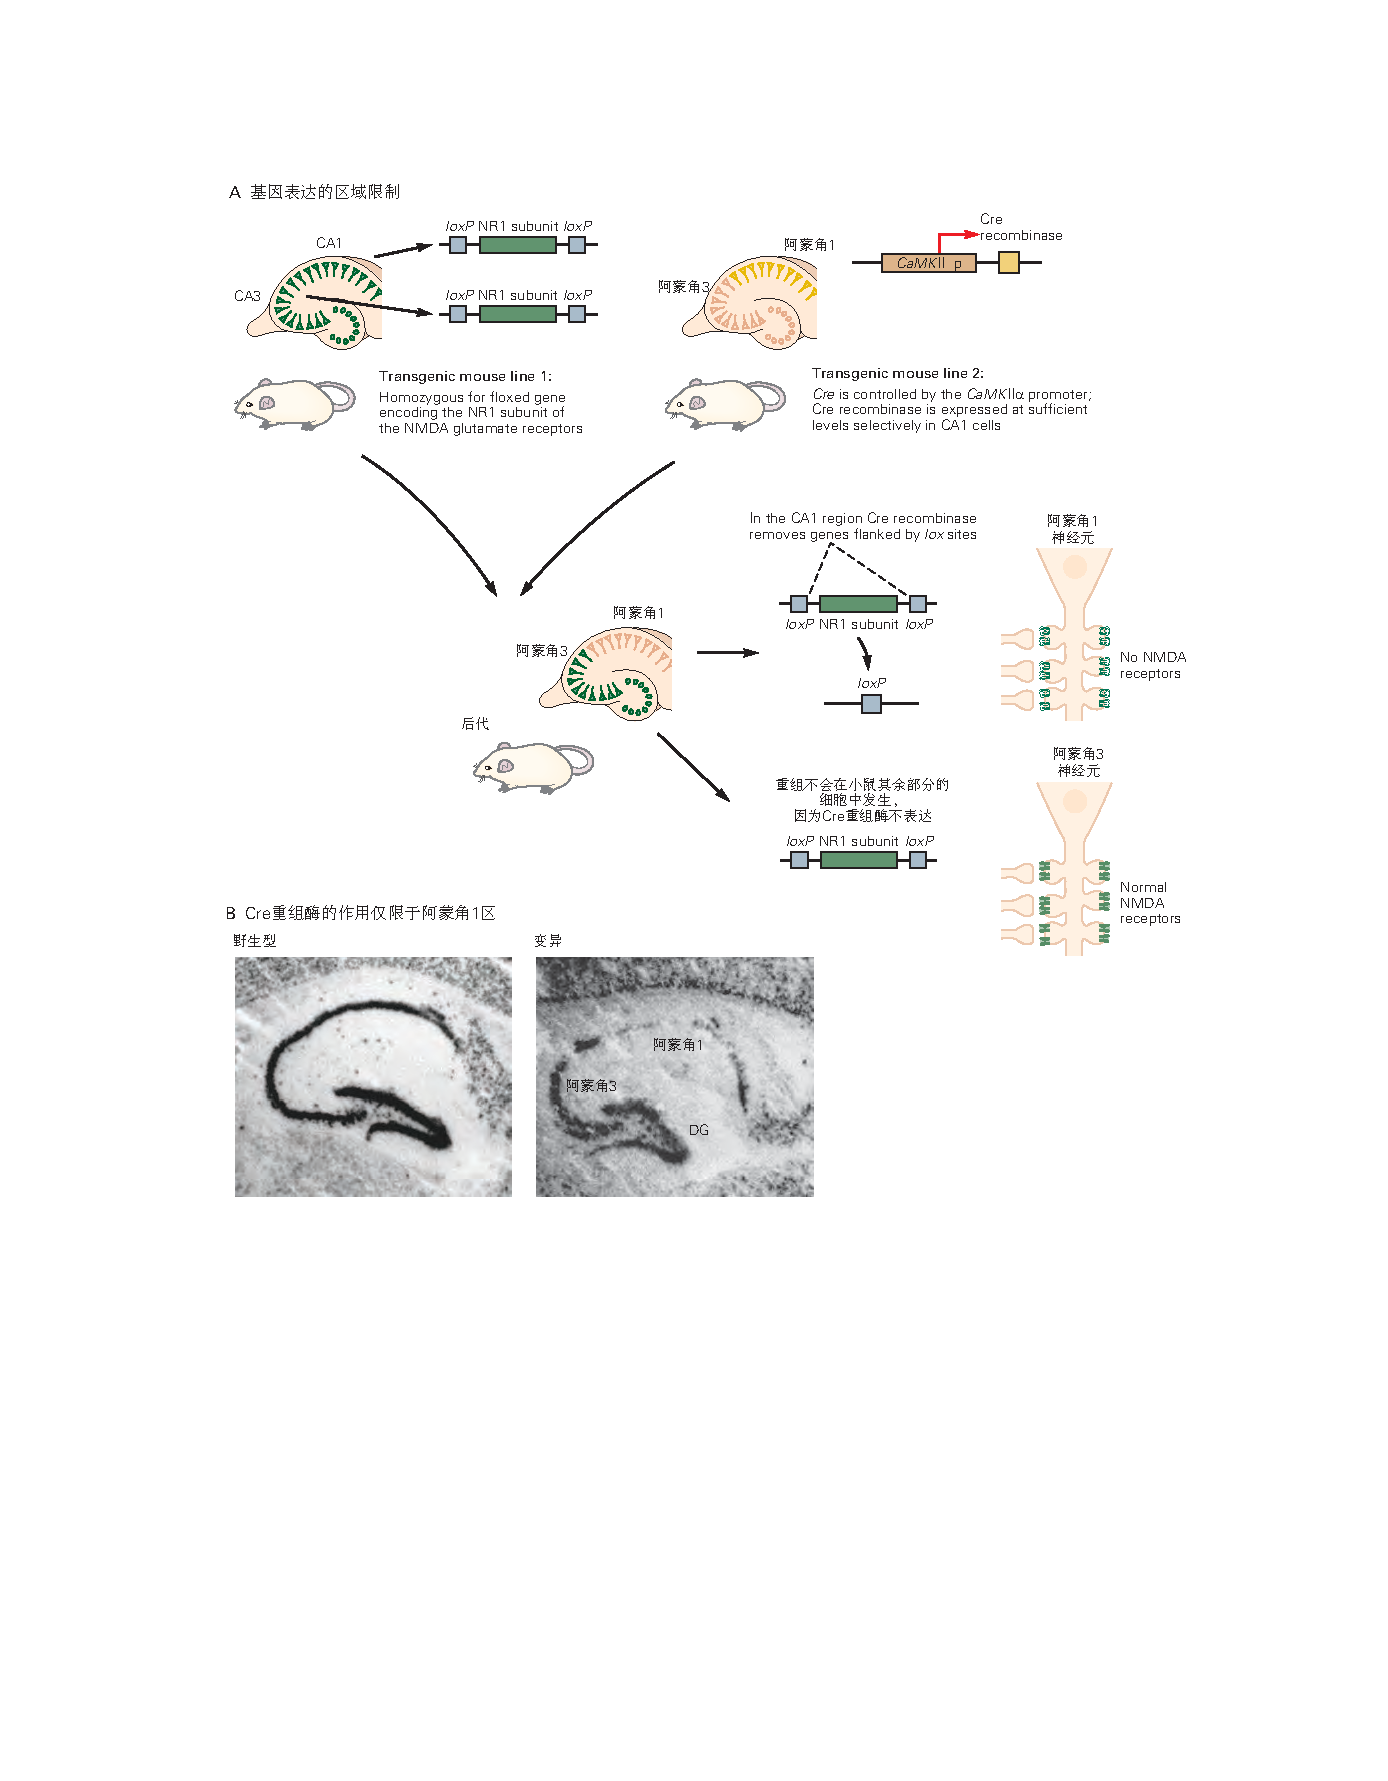
\includegraphics[width=1.0\linewidth]{chap02/fig_2_8}
	\caption{用于选择性区域基因敲除的Cre/loxP系统。
		\textbf{A.} 培育了一种小鼠系,其中编码\textit{N-甲基-D-天冬氨酸}受体NR1亚基的基因两侧有loxP遗传元件(转基因小鼠系1)。
		然后将这些所谓的“floxed NR1”小鼠与第二系小鼠杂交,其中编码Cre重组酶的转基因置于细胞类型或组织类型特异性转录启动子的控制下(转基因小鼠系2)。
		在本实施例中,来自\textit{钙/钙调蛋白依赖性蛋白激酶 2}a基因的启动子用于驱动Cre基因的表达。
		在携带Cre重组酶转基因的Floxy基因纯合的子代中,仅在驱动Cre表达的启动子活性的细胞类型中,通过Cre介导的loxP重组,Floxy的基因将被删除。
		\textbf{B.} 原位杂交用于检测野生型和突变小鼠海马切片中NR1亚基的\textit{信使核糖核酸},这些小鼠含有两个固定的NR1等位基因,并在\textit{钙/钙调蛋白依赖性蛋白激酶 2}a启动子的控制下表达Cre重组酶。
		在突变小鼠中,NR1的\textit{信使核糖核酸}表达(暗染色)在海马\textit{阿蒙角}1区显著减少,但在\textit{阿蒙角}3和\textit{齿状回}保持正常\cite{tsien1996essential}。}
	\label{fig:2_8}
\end{figure}



\begin{proposition}[神经解剖学导航术语] \label{box:2_3}
	
	\quad \quad 转基因在苍蝇和老鼠中的引入
	
	\quad \quad 通过将\textit{脱氧核糖核酸}注射到新受精卵的细胞核中,可以在小鼠体内实验性地引入基因(图~\ref{fig:2_10})。
	在一些注射的卵子中,新基因或转基因被整合到其中一条染色体上的随机位点。
	由于胚胎处于单细胞阶段,整合的基因被复制并最终进入动物的所有(或几乎所有)细胞,包括种系。
	
	\quad \quad 通过将用于产生色素的基因注射到从白化病菌株获得的蛋中而拯救的外壳颜色标记基因来说明基因掺入。
	有色素斑块的小鼠表明\textit{脱氧核糖核酸}的成功表达。
	通过测试注射动物的\textit{脱氧核糖核酸}样本,证实了转基因的存在。
	
	\quad \quad 在苍蝇身上也使用了类似的方法。将待注射的\textit{脱氧核糖核酸}克隆到可转座元件(P元件)中。
	当注射到胚胎中时,\textit{脱氧核糖核酸}被插入生殖细胞核的\textit{脱氧核糖核酸}中。
	P元件可以被工程化以在特定时间和特定细胞中表达基因。
	转基因可以是恢复突变体功能的野生型基因,或者是改变其他基因表达或编码特异性改变的蛋白质的设计基因。
	
\end{proposition}


\begin{figure}[htbp]
	\centering
	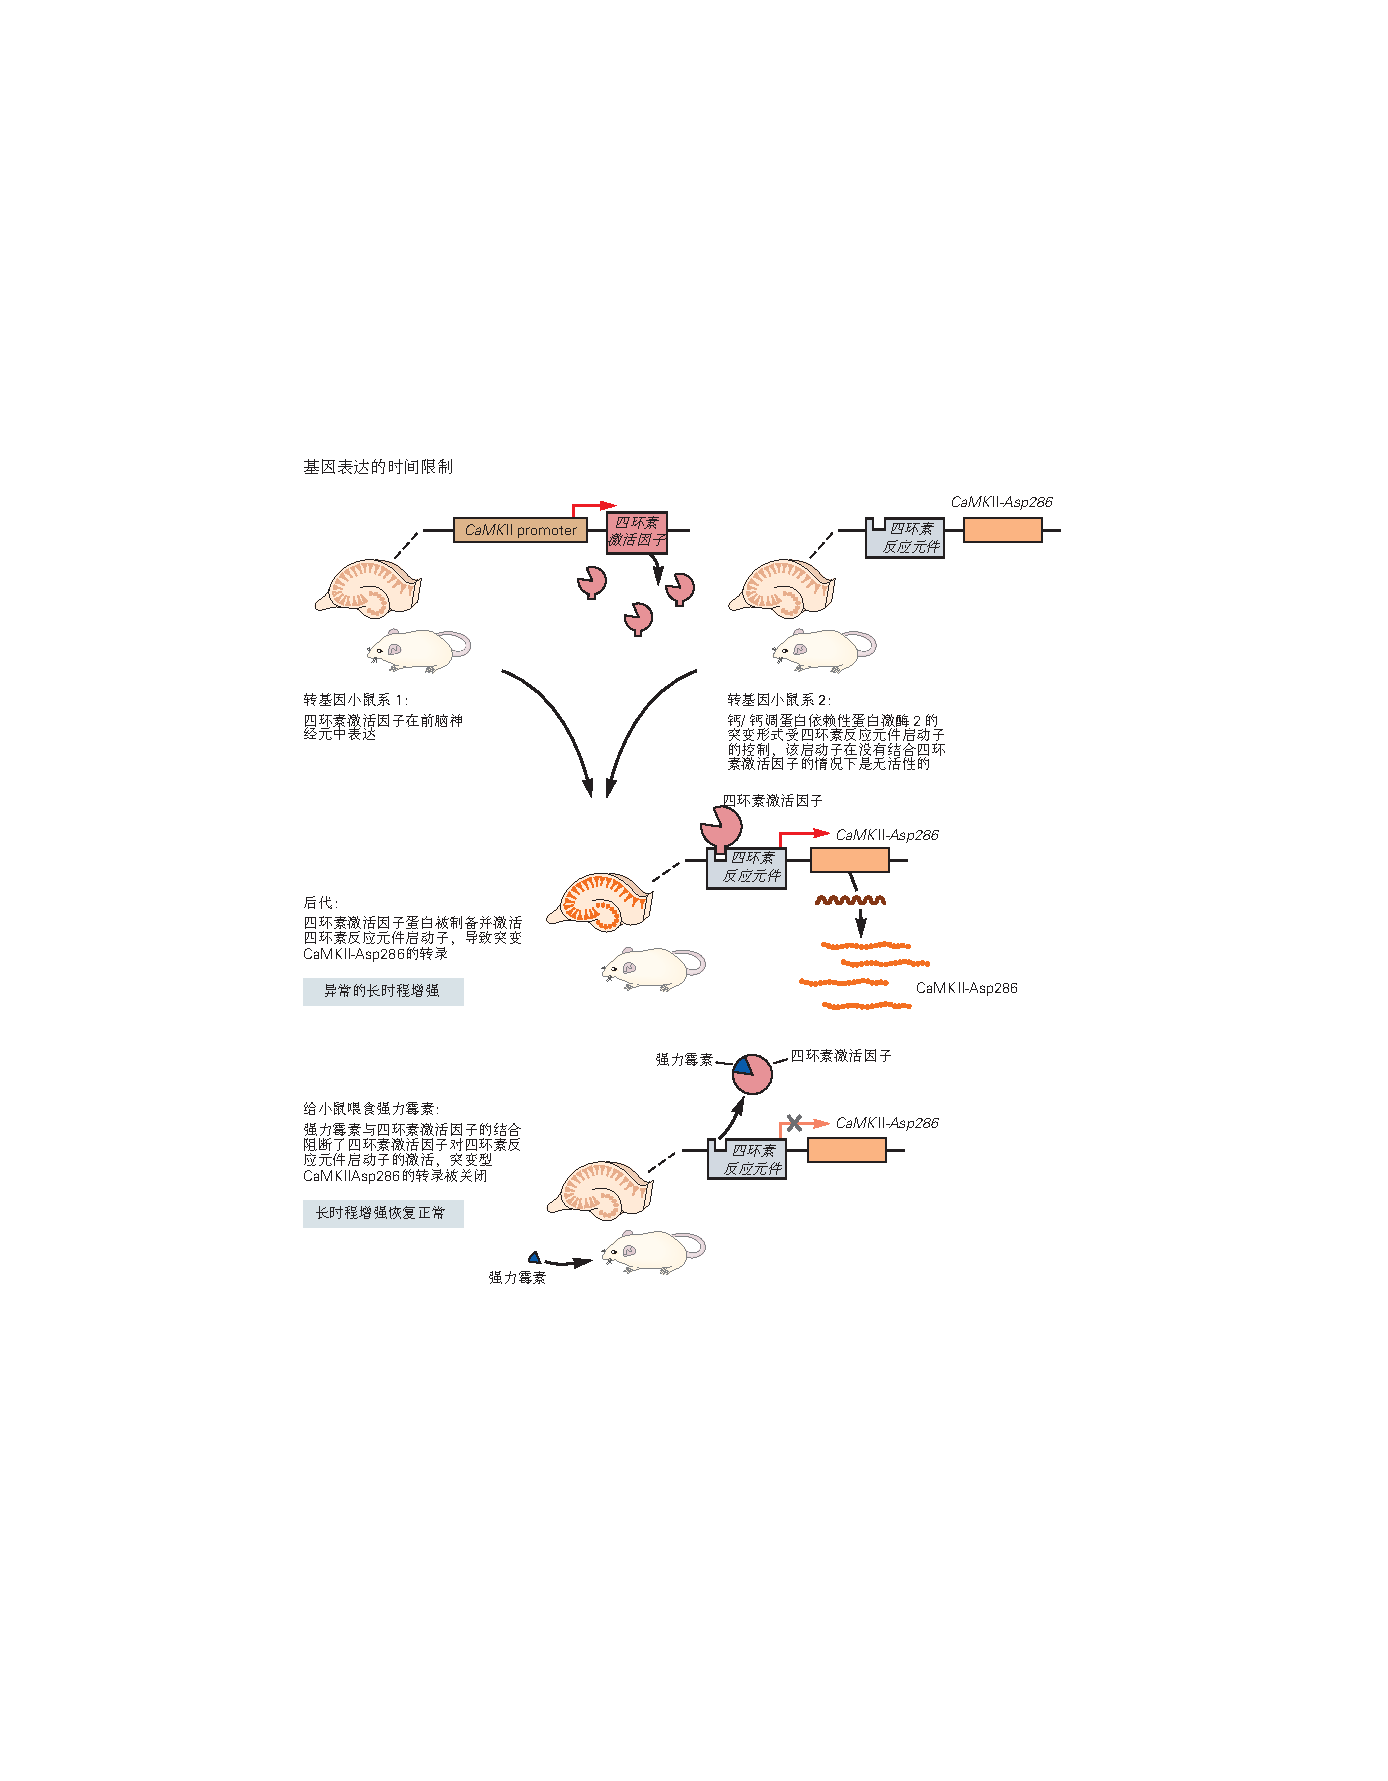
\includegraphics[width=0.87\linewidth]{chap02/fig_2_9}
	\caption{四环素系统用于转基因表达的时间和空间调控。培育了两个独立的转基因小鼠系。
		一个系在\textit{钙/钙调蛋白依赖性蛋白激酶 2}a启动子的控制下表达\textit{四环素激活因子},这是一种结合了识别细菌\textit{四环素反应元件}操纵子的细菌转录因子的工程蛋白。
		第二条线包含一个感兴趣的转基因(这里编码一种组成型活性形式的\textit{钙/钙调蛋白依赖性蛋白激酶 2}),它使激酶在没有\ce{Ca^2+}的情况下持续活性,其表达受\textit{四环素反应元件}的控制。
		当这两个系交配时,后代以仅限于前脑的模式表达\textit{四环素激活因子}蛋白。
		当\textit{四环素激活因子}蛋白与\textit{四环素反应元件}结合时,它将激活感兴趣的下游基因的转录。
		给后代服用四环素(或多西环素)与\textit{四环素激活因子}蛋白结合,并引起构象变化,导致该蛋白与\textit{四环素反应元件}解除结合,阻断转基因表达。
		通过这种方式,小鼠将在前脑中表达\textit{钙/钙调蛋白依赖性蛋白激酶 2}–Asp286,并且可以通过向小鼠施用多西环素来阻断这种表达\cite{mayford1996control}。}
	\label{fig:2_9}
\end{figure}


\begin{figure}[htbp]
	\centering
	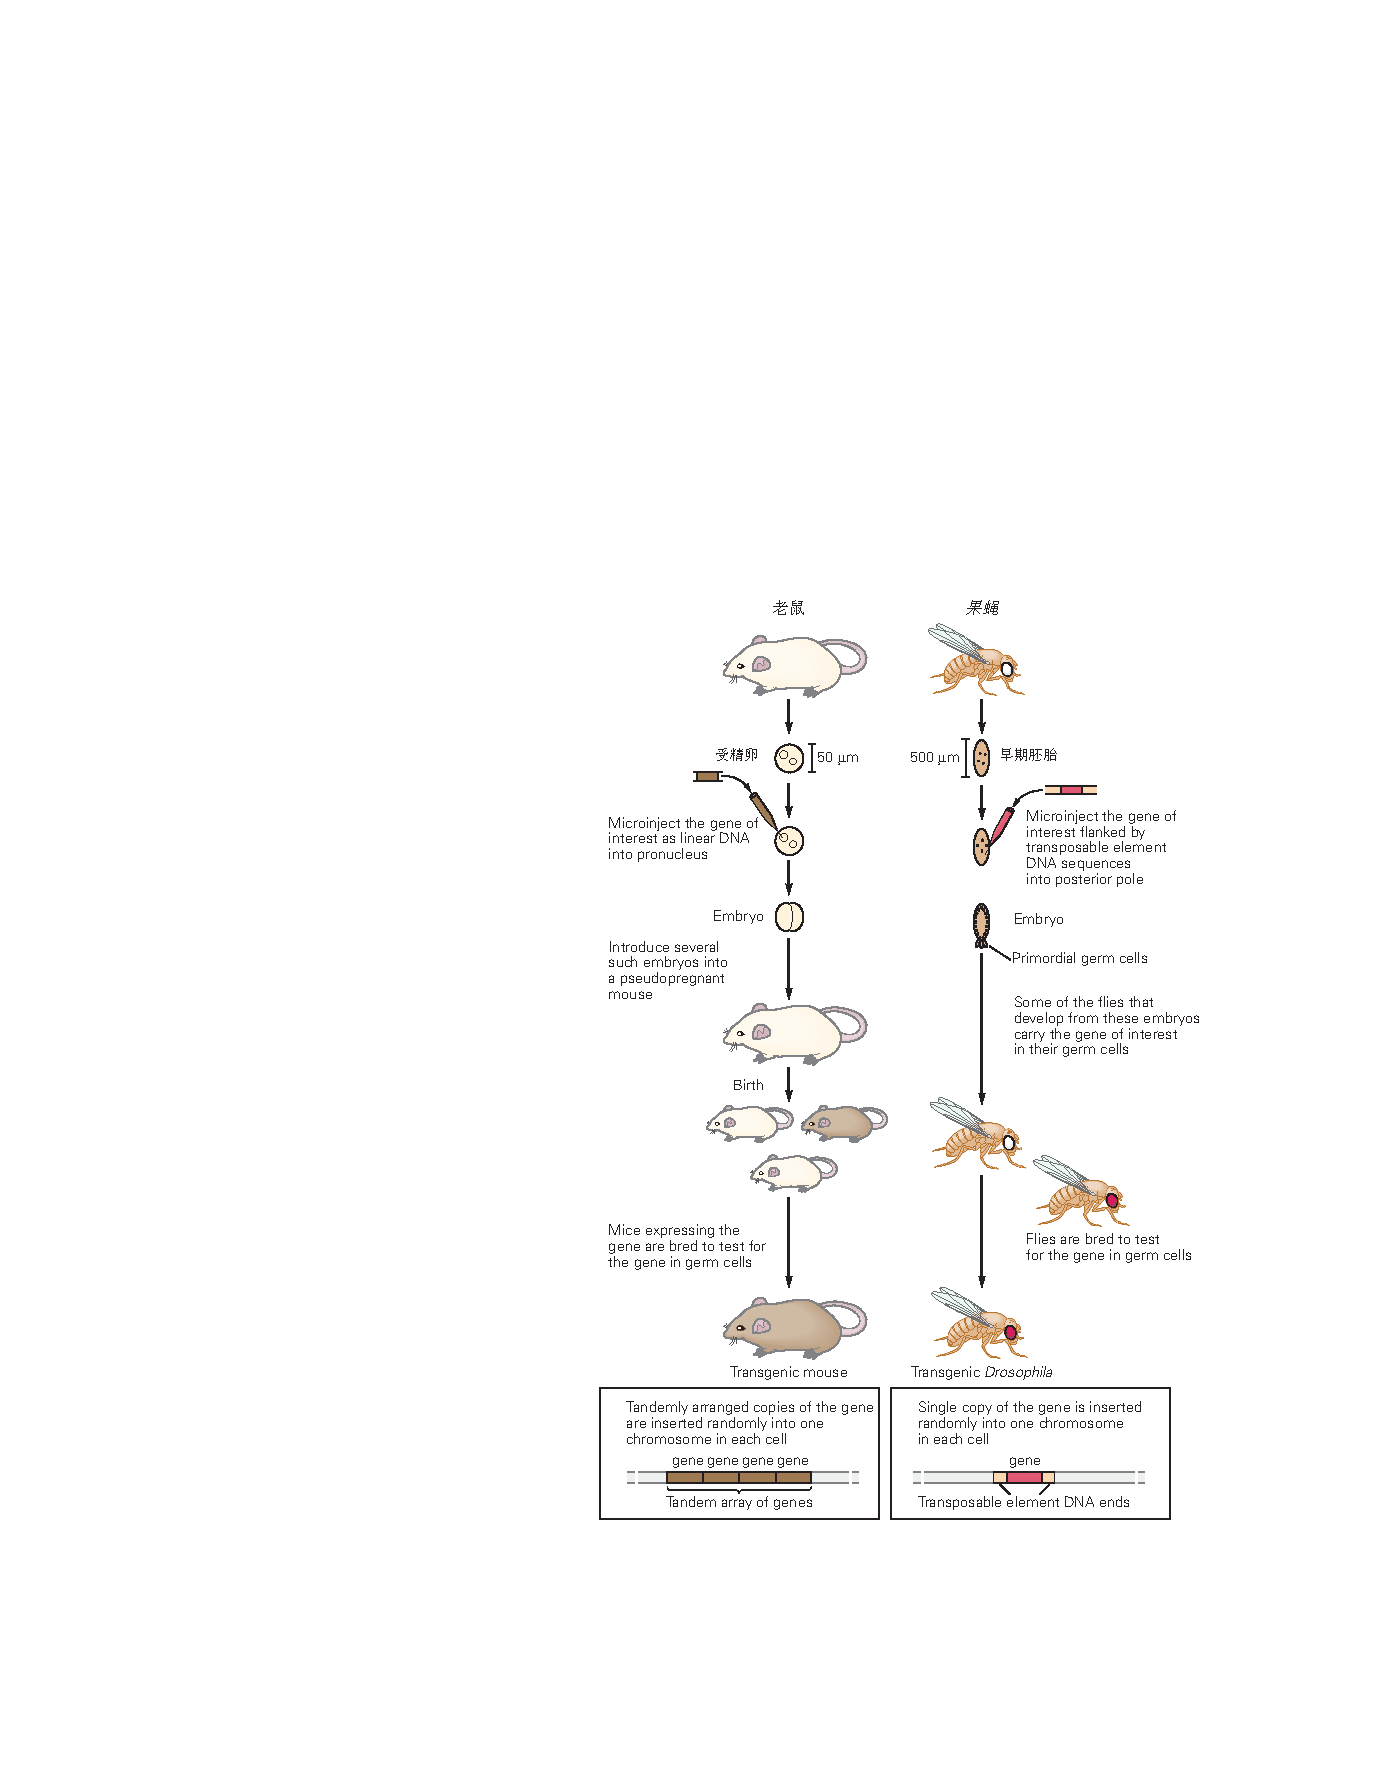
\includegraphics[width=0.75\linewidth]{chap02/fig_2_10}
	\caption{产生转基因小鼠和苍蝇。
		在这里,注射到小鼠体内的基因会导致毛色的变化,而注射到苍蝇体内的基因则会导致眼睛颜色的变化。
		在这两个物种的一些转基因动物中,\textit{脱氧核糖核酸}被插入不同细胞的不同染色体位点(见底部的插图)\cite{alberts2017molecular}。}
	\label{fig:2_10}
\end{figure}




我们对行为的昼夜节律控制的遗传基础有一个特别完整的了解。
动物的昼夜节律将某些行为与与太阳升起和落下相关的 24 小时周期联系起来。
昼夜节律调节的核心是一个在 24 小时周期内振荡的内在生物钟。
由于时钟的内在周期性,即使在没有光或其他环境影响的情况下,昼夜节律行为也会持续存在。


生物钟可以重新设置,这样昼夜循环的变化最终会导致内在振荡器发生匹配的变化,这是任何正在从时差反应中恢复过来的旅行者都熟悉的现象。
时钟由眼睛传输到大脑的光驱动信号重置。
最后,时钟驱动特定行为的效应通路,例如睡眠和运动。


\textit{本泽}的团队搜索了数千只突变果蝇,以寻找由于指导昼夜节律振荡的基因发生突变而无法遵循昼夜节律的稀有果蝇。
从这项工作中,人们对生物钟的分子机制有了初步的了解。
周期或每个基因的突变影响果蝇内部时钟产生的所有昼夜节律行为。


有趣的是,每个突变都可以通过多种方式改变生物钟(图~\ref{fig:2_11})。
心律失常的\textit{节律基因}突变果蝇在任何行为中都没有表现出明显的内在节律,缺乏\textit{节律基因}的所有功能,因此\textit{节律基因}对节律行为至关重要。
维持基因某些功能的突变会导致节律异常。
长日等位基因产生 28 小时的行为周期,而短日等位基因产生 19 小时的行为周期。
因此\textit{节律基因}不仅是时钟的重要组成部分,它实际上是一个计时员,其活动可以改变时钟运行的速率。


\begin{figure}[htbp]
	\centering
	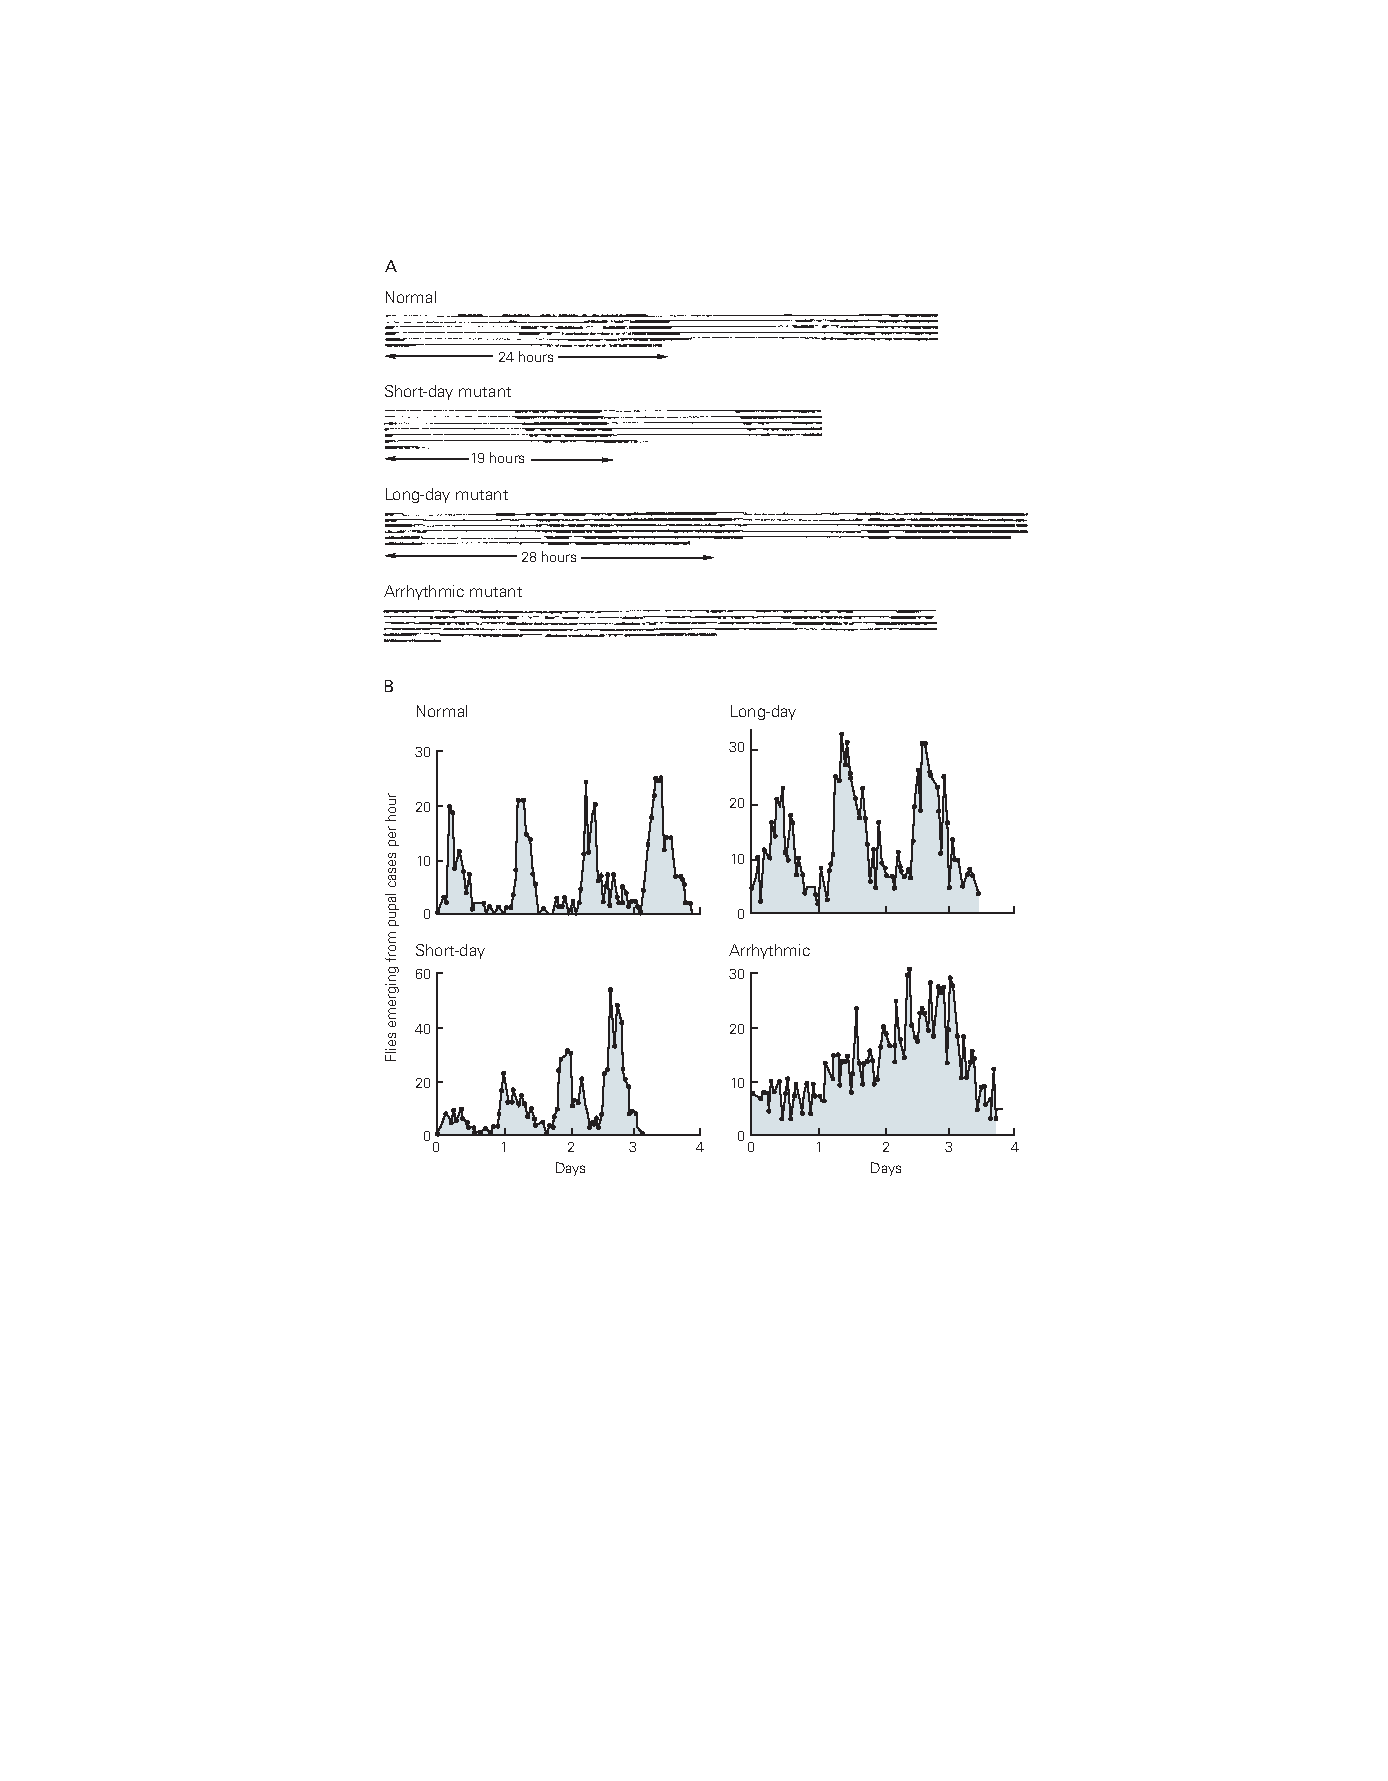
\includegraphics[width=0.8\linewidth]{chap02/fig_2_11}
	\caption{一个基因控制着果蝇行为的昼夜节律。
		周期或每个基因的突变会影响果蝇内部时钟调节的所有昼夜节律行为\cite{konopka1971clock}。
		\textbf{A.} 正常果蝇和\textit{节律基因}突变体的三种菌株的运动节律:短日照、长日照和心律失常。
		将苍蝇从 12 小时光照和 12 小时黑暗的循环转变为持续黑暗,然后在红外光下监测活动。
		记录中的粗段表示活动。
		\textbf{B.} 正常的成年苍蝇种群以周期性的方式从它们的蛹壳中出现,即使在持续的黑暗中也是如此。
		这些图显示了在持续黑暗的 4 天期间每小时出现的苍蝇数量(四个种群中的每一个)。
		出现没有任何可辨别的节律的心律失常突变种群。}
	\label{fig:2_11}
\end{figure}


\textit{节律基因}突变体除了昼夜节律行为的改变外没有主要的不利影响。
这一观察很重要,因为在发现之前,许多人质疑是否可能存在动物生理需要不需要的真正“行为基因”。
\textit{节律基因}似乎确实是这样一种“行为基因”。


\textit{节律基因}是如何保持时间的?
蛋白质产物\textit{周期蛋白}是一种转录调节因子,可影响其他基因的表达。
\textit{周期蛋白}的水平全天受到监管。
清晨,\textit{周期蛋白}及其\textit{信使核糖核酸}较低。
在一天中,\textit{周期蛋白}\textit{信使核糖核酸}和蛋白质积累,在黄昏后和夜间达到峰值水平。
然后水平下降,在下一个黎明前下降。
这些观察为昼夜节律之谜提供了答案,即一个中央调节器在一天中出现和消失。
但它们也不令人满意,因为它们只是将问题往后推了一步,即什么是\textit{周期蛋白}循环?
这个问题的答案需要发现额外的\textit{时钟基因},这些基因在果蝇和老鼠身上都有发现。


受到果蝇昼夜节律筛查成功的鼓舞,\textit{约瑟夫$\cdot$高桥}在 1990 年代开始在老鼠身上进行类似但劳动密集型得多的基因筛查。
他筛选了数百只突变小鼠,寻找昼夜运动周期发生改变的罕见个体,并发现了一个他称之为\textit{时钟基因}突变。
当\textit{时钟基因}突变的纯合小鼠被转移到黑暗中时,它们最初会经历极长的昼夜节律周期,然后完全失去昼夜节律(图~\ref{fig:2_12})。
因此,\textit{时钟基因}似乎可以调节昼夜节律的两个基本特性:昼夜节律周期的长度和在没有感觉输入的情况下节律性的持久性。
这些特性在概念上与果蝇中\textit{节律基因}基因的特性相同。


\begin{figure}[htbp]
	\centering
	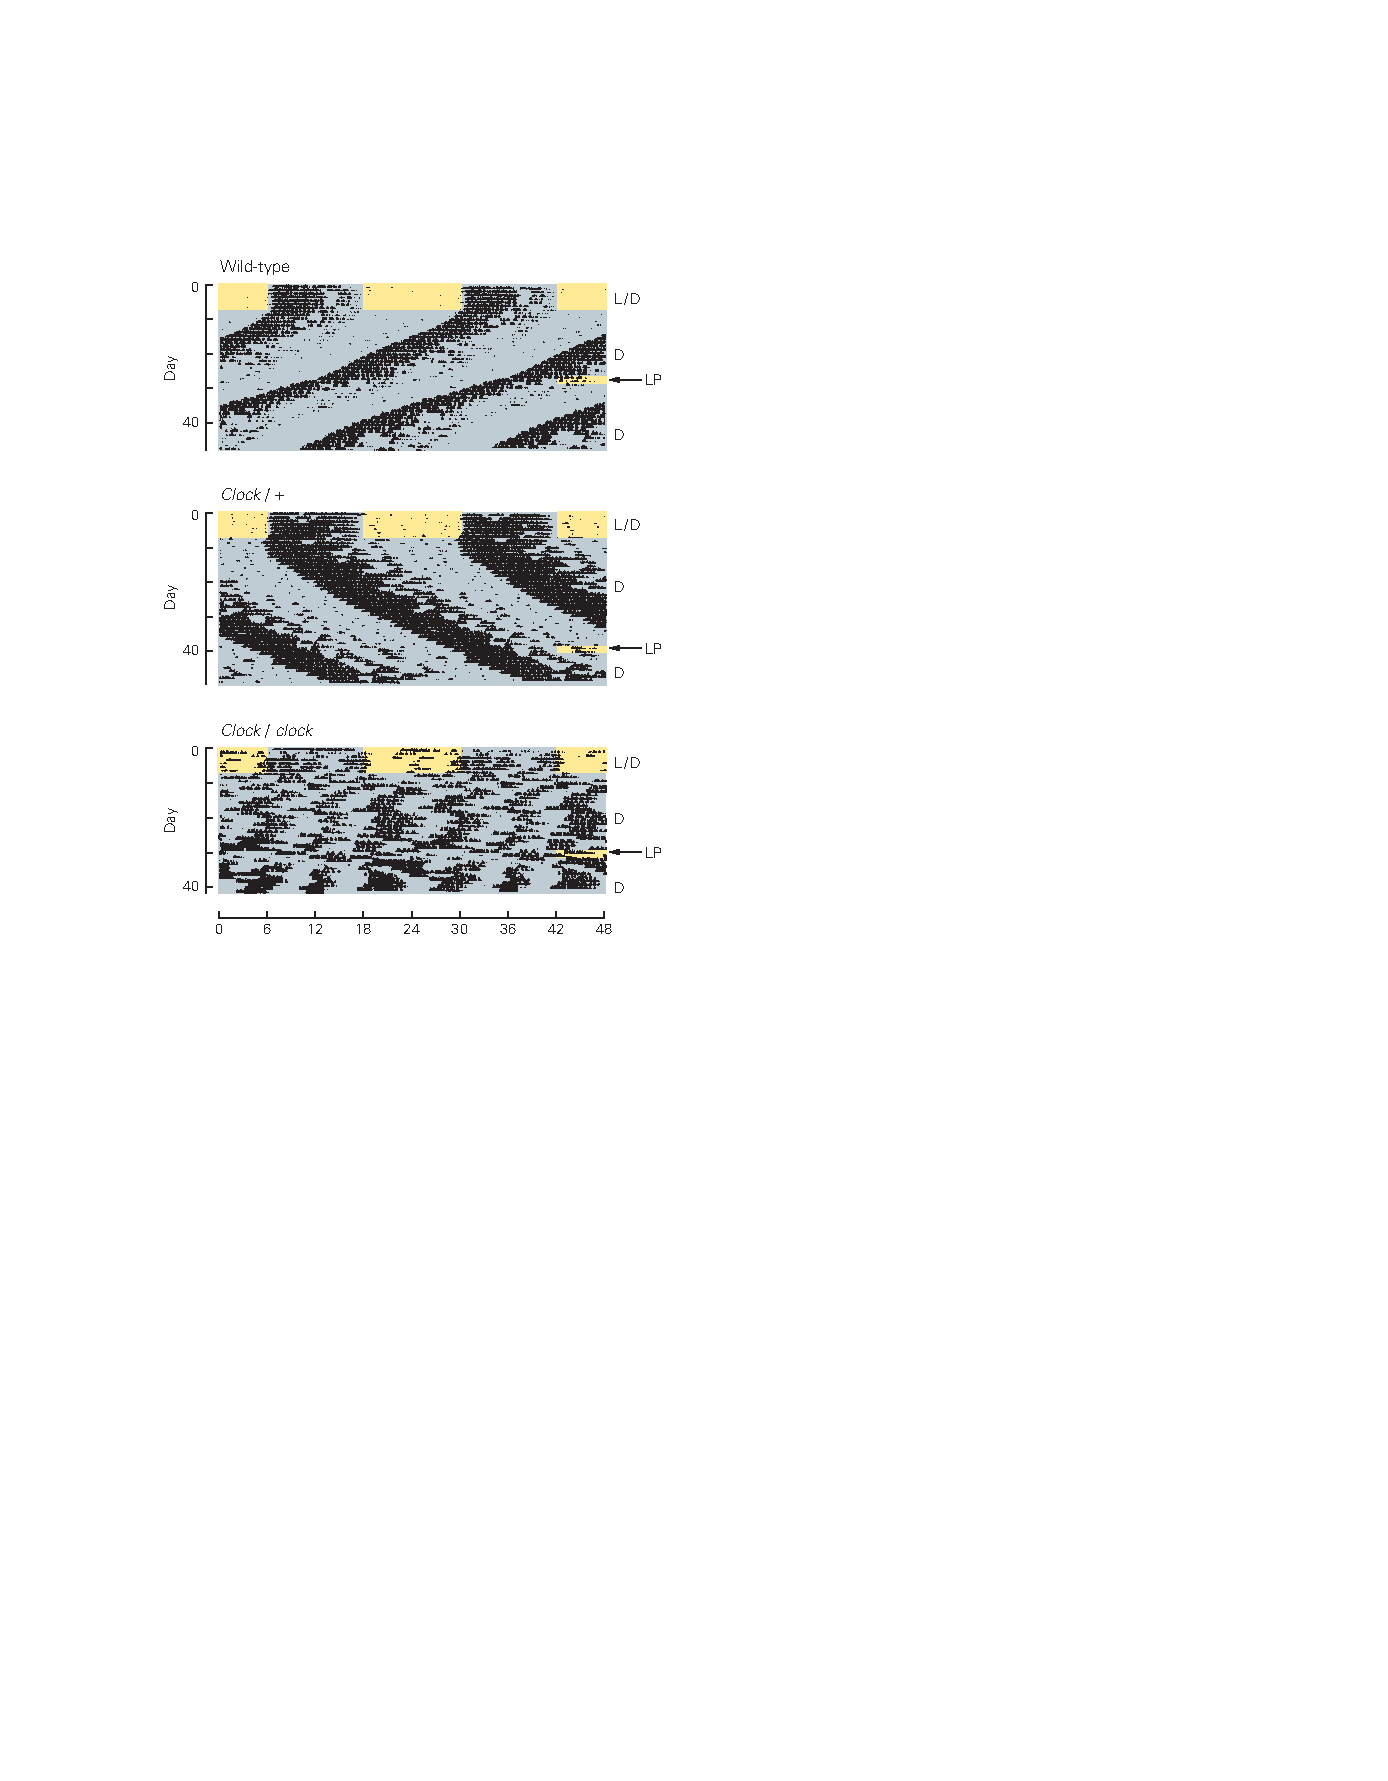
\includegraphics[width=0.55\linewidth]{chap02/fig_2_12}
	\caption{\textit{时钟基因}对小鼠昼夜节律的调节。
		记录显示了三种动物的运动活动期:野生型、杂合型和纯合型。
		所有动物在前7天保持12小时的亮暗循环,然后转移到恒定黑暗。
		之后,他们被暴露在6小时的\textit{光照周期}中以重置节奏。
		野生型小鼠的昼夜节律具有23.1小时的周期。
		杂合时钟/+小鼠的周期为24.9小时。
		纯合子时钟/时钟小鼠在转移到恒定黑暗时经历昼夜节律性的完全丧失,并在光照期后短暂表达28.4小时的节律\cite{takahashi1994forward}。}
	\label{fig:2_12}
\end{figure}


小鼠\textit{时钟基因}与果蝇中的\textit{节律基因}基因一样,编码一个转录调节器,其活动在一天中波动。
小鼠\textit{时钟蛋白}和果蝇\textit{周期蛋白}也共享一个称为 PAS 结构域的结构域,这是转录调节因子子集的特征。
这一观察表明,相同的分子机制(PAS 结构域转录调节的振荡)控制着果蝇和小鼠的昼夜节律。


更重要的是,对果蝇和小鼠的平行研究表明,相似的转录调节因子组会影响这两种动物的生物钟。
在克隆小鼠\textit{时钟基因}后,克隆了一个果蝇昼夜节律基因,发现它与小鼠时钟的关系比\textit{节律基因}。
在另一项研究中,一种与 fly \textit{节律基因}相似的小鼠基因被鉴定并通过反向遗传学灭活。
突变小鼠有昼夜节律缺陷,就像每个突变体都会飞一样。 
换句话说,果蝇和小鼠都使用\textit{时钟基因}和每个基因来控制它们的昼夜节律。
一组基因,而不是一个基因,是生物钟的保守调节剂。


这些基因的表征导致了对昼夜节律分子机制的理解,并戏剧性地证明了这些机制在果蝇和小鼠中的相似性。
在果蝇和小鼠中,\textit{时钟蛋白}都是一种转录激活因子。 
它与伴侣蛋白一起控制决定运动活动水平等行为的基因的转录。
\textit{时钟蛋白}及其伙伴还刺激\textit{节律基因}基因的转录。
然而,\textit{周期蛋白}抑制\textit{时钟蛋白}刺激每个基因表达的能力,因此随着 \textit{周期蛋白}的积累,每个转录下降(图~\ref{fig:2_13})。
24 小时周期的出现是因为\textit{周期蛋白}的积累和激活在\textit{节律基因}转录后延迟了许多小时,这是\textit{周期蛋白}磷酸化、\textit{周期蛋白}不稳定性以及与其他循环蛋白相互作用的结果。


\begin{figure}[htbp]
	\centering
	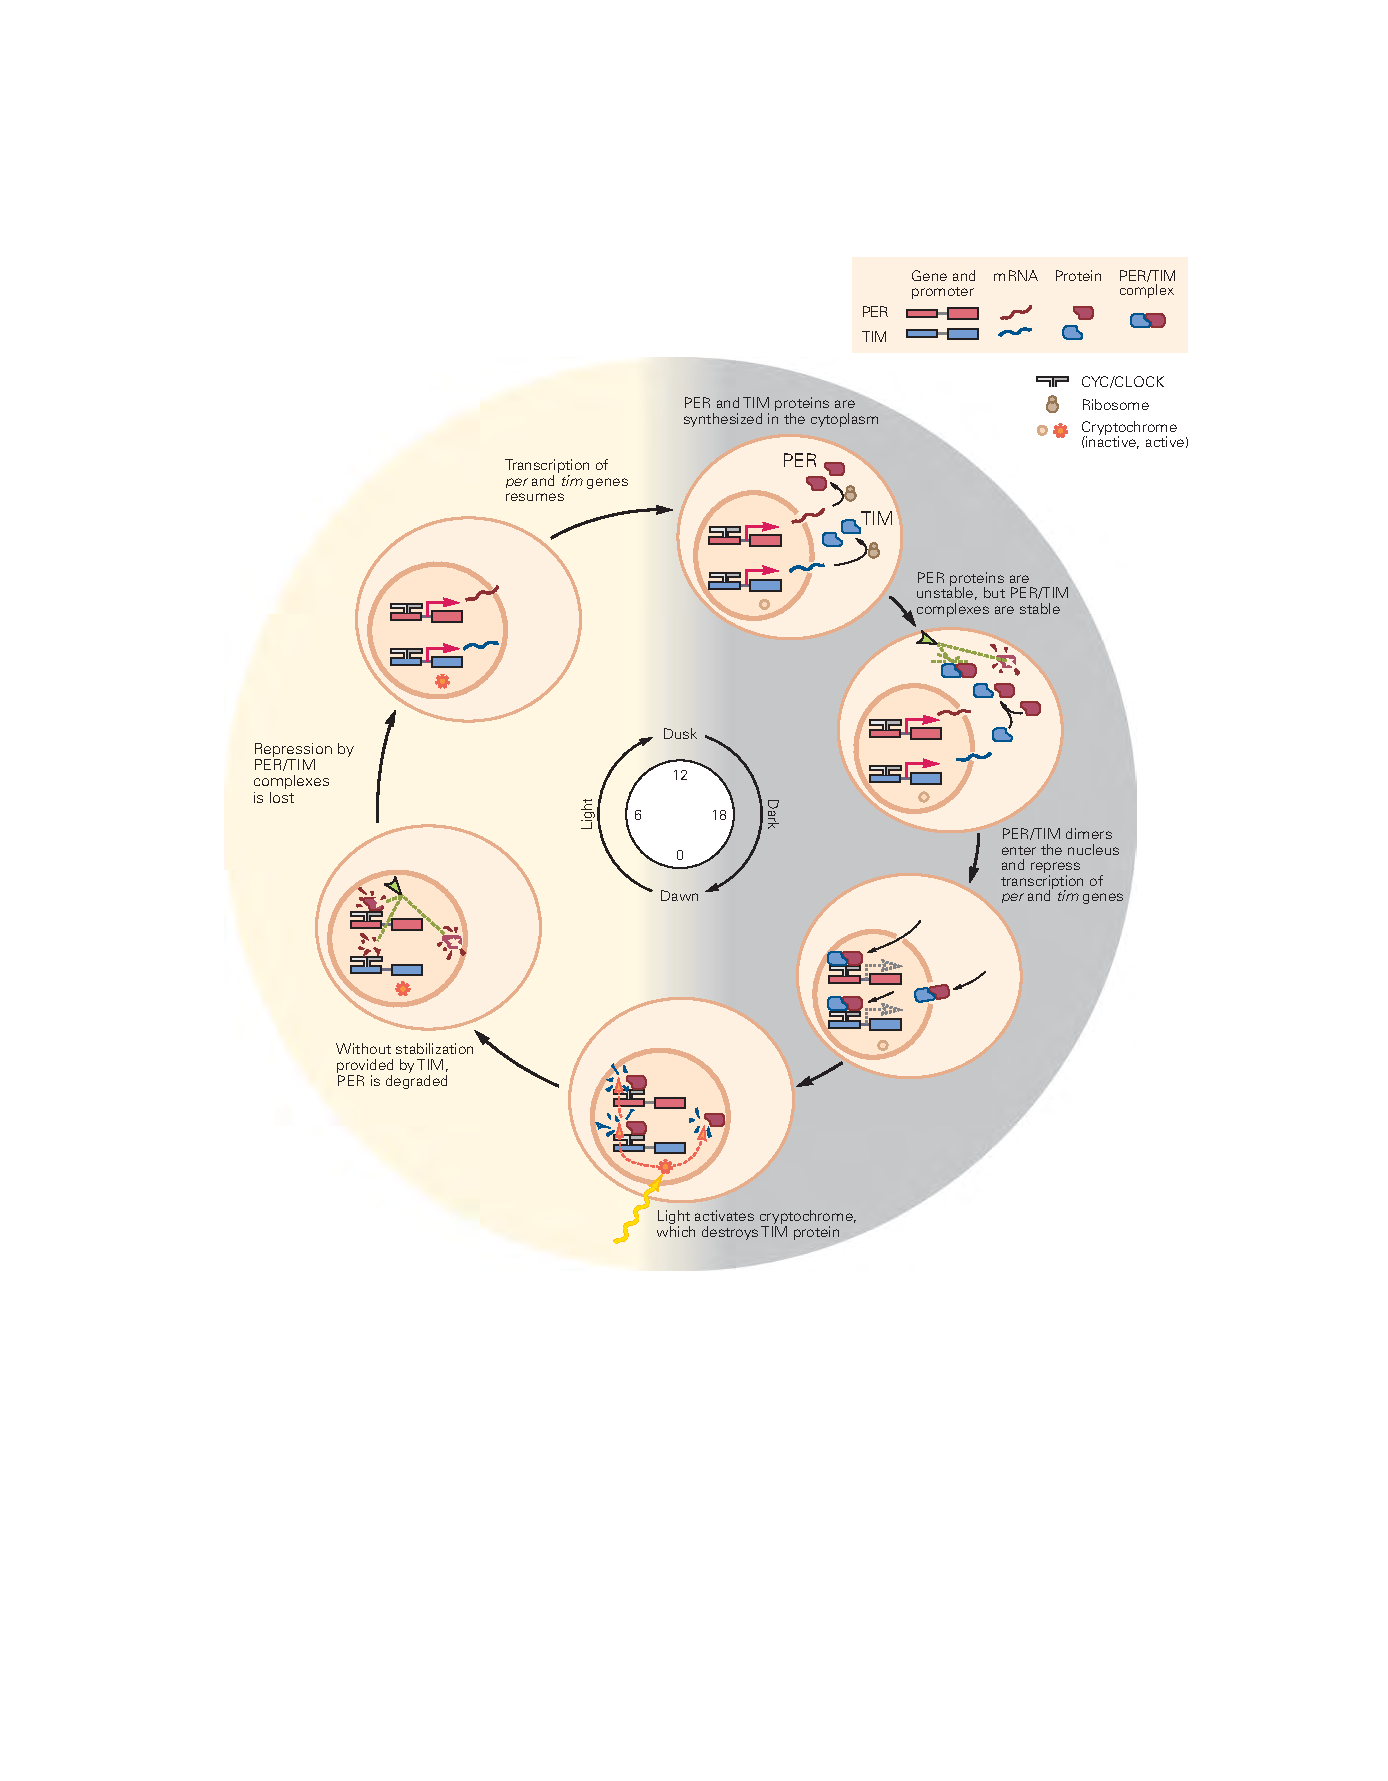
\includegraphics[width=1.0\linewidth]{chap02/fig_2_13}
	\caption{驱动昼夜节律的分子事件。
		控制生物钟的基因受两种核蛋白\textit{周期蛋白}和\textit{无节律蛋白}的调节。
		这些蛋白质慢慢积累,然后相互结合形成二聚体。
		一旦它们形成二聚体,它们就会进入细胞核并关闭包括它们自己在内的昼夜节律基因的表达。
		它们通过抑制刺激\textit{节律基因}和\textit{无节律基因}转录的\textit{时钟蛋白}和 CYCLE 来实现。
		\textit{周期蛋白}非常不稳定;
		其中大部分降解得如此之快,以至于它永远没有机会抑制每个转录的时钟依赖性。 
		\textit{周期蛋白}的降解受不同蛋白激酶的至少两种不同磷酸化事件的调节。
		当\textit{周期蛋白}与\textit{无节律蛋白}结合时,\textit{周期蛋白}受到保护免于降解。 
		随着\textit{时钟蛋白}驱动越来越多的\textit{节律基因}和\textit{无节律基因}表达,足够的\textit{周期蛋白}和\textit{无节律蛋白}最终积累到两者可以结合并稳定彼此,此时它们进入细胞核,在那里它们自身的转录受到抑制。
		结果,\textit{节律基因}和\textit{无节律基因}的\textit{信使核糖核酸}水平下降; 此后,\textit{周期蛋白}和\textit{无节律蛋白}水平下降,\textit{时钟蛋白}可以(再次)驱动\textit{节律基因}和\textit{无节律基因}\textit{信使核糖核酸}的表达。
		在白天,\textit{无节律蛋白}被光调节的信号通路(包括隐花色素)降解,因此\textit{周期蛋白}/\textit{无节律蛋白}复合物仅在夜间形成。
		\textit{时钟蛋白}诱导\textit{周期蛋白}和\textit{无节律蛋白}表达,但被\textit{周期蛋白}和 \textit{无节律蛋白}蛋白抑制。}
	\label{fig:2_13}
\end{figure}


\textit{节律基因}、\textit{时钟基因}和相关基因的分子特性产生了昼夜节律所必需的所有特性。

1. 昼夜节律基因转录随24小时周期变化:夜间\textit{周期蛋白}活性高;
\textit{时钟蛋白}白天活跃度很高。


2. 昼夜节律基因是相互影响\textit{信使核糖核酸}水平的转录因子,产生振荡。
\textit{时钟蛋白}按转录激活,\textit{周期蛋白}抑制\textit{时钟蛋白}功能。


3. 昼夜节律基因还控制其他基因的转录,进而影响许多下游反应。
例如,在果蝇中,神经肽基因 pdf 控制运动活动水平。


4. 这些基因的振荡可以被光重置。


2017 年诺贝尔生理学或医学奖授予了\textit{杰弗里$\cdot$霍尔}、\textit{迈克尔$\cdot$罗斯巴什}和\textit{迈克尔$\cdot$杨},表彰了对这种分子钟机制的详细阐述。


相同的遗传网络控制着人类的昼夜节律。
患有晚期睡眠阶段综合症的人具有较短的 20 天周期和极端早睡、早起的“早晨云雀”表型。
\textit{路易斯$\cdot$普塔切克}和\textit{傅颖慧}发现这些个体的每个基因都具有人类突变。
这些结果表明,行为基因从昆虫到人类都是保守的。 
晚期睡眠时相综合症在睡眠章节(第~\ref{chap:chap44}~章)中进行了讨论。



\subsection{蛋白激酶的自然变异调节果蝇和蜜蜂的活性}

在前面描述的昼夜节律的遗传学研究中,随机诱变被用来识别生物过程中感兴趣的基因。
所有正常个体都有\textit{节律基因}、\textit{时钟基因}和相关基因的功能拷贝;
只有在诱变后才会产生不同的等位基因。
另一个关于基因在行为中的作用的更微妙的问题是,哪些基因变化可能导致正常个体的行为变异。
\textit{玛尔拉$\cdot$索科洛夫斯基}及其同事的工作导致鉴定出第一个与一个物种中正常个体的行为变异相关的基因。


果蝇幼虫的活动水平和运动方式各不相同。
一些称为漫游者的幼虫会长距离移动(图~\ref{fig:2_14})。
其他人称为保姆,相对静止。
从野外分离出的果蝇幼虫可以是漫游者或保育者,表明这些是自然变异而不是实验室诱导的突变。
这些特征是可遗传的;
流浪者父母有流浪者后代,保姆父母有保姆后代。


\begin{figure}[htbp]
	\centering
	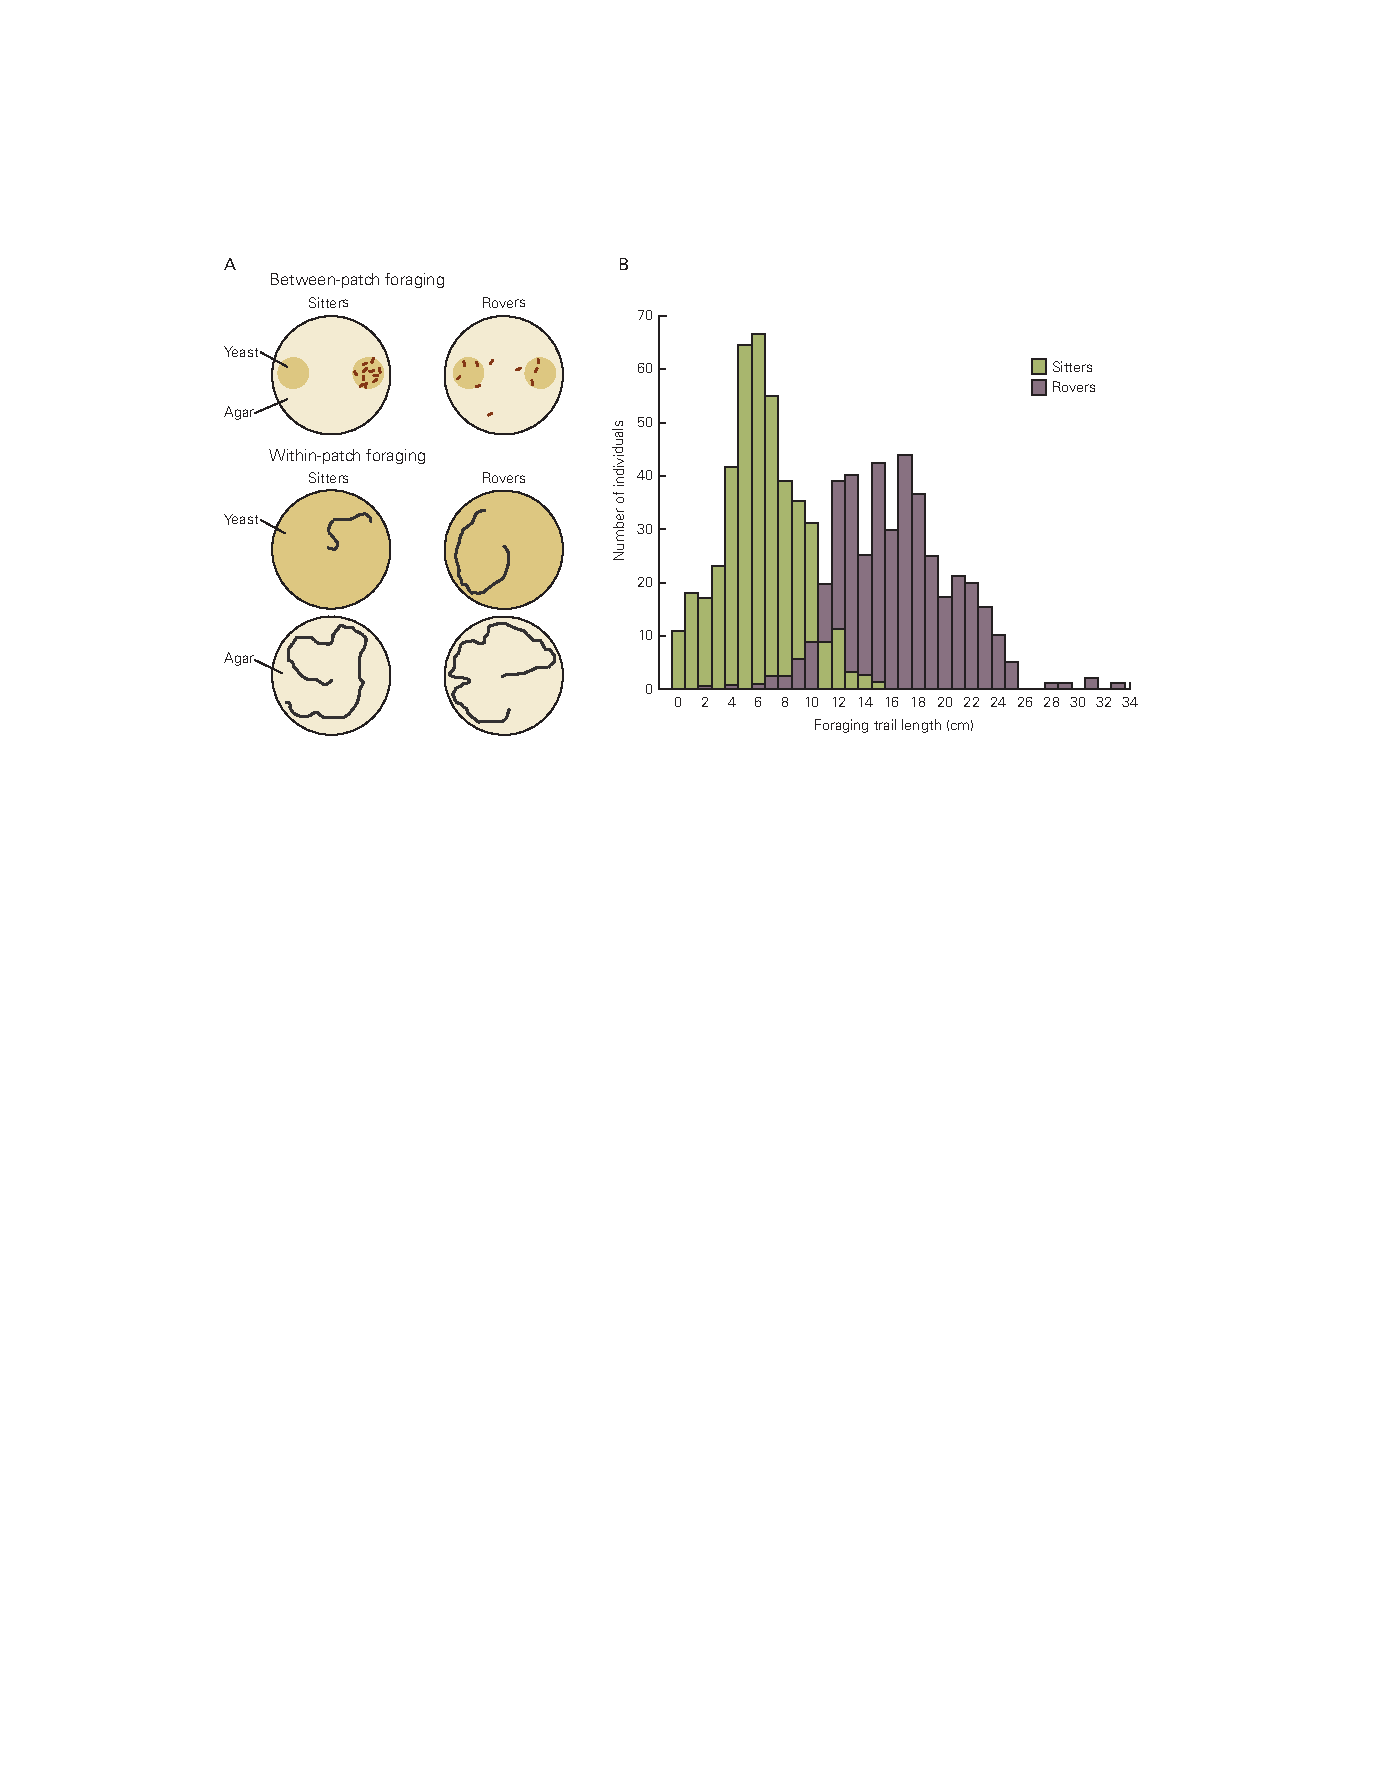
\includegraphics[width=0.95\linewidth]{chap02/fig_2_14}
	\caption{\textit{果蝇漫游者}和\textit{保姆幼虫}在享用酵母时的觅食行为不同\cite{sokolowski2001drosophila}。
		\textbf{A.} 漫游型幼虫从一块地移动到另一块地,而保姆型幼虫在一块地上停留很长时间。
		当在一块地里觅食时,漫游者幼虫比保姆幼虫移动得更多。
		仅在琼脂上,漫游者和保姆幼虫的移动速度相等。
		\textbf{B.} 当漫游者在一片食物中觅食时,它们的踪迹长度比\textit{保姆幼虫}长(踪迹长度是在5分钟内测量的)。
		这种觅食行为的差异映射到一个单一的蛋白激酶基因,该基因在不同的苍蝇幼虫中的活性不同。}
	\label{fig:2_14}
\end{figure}


\textit{索科洛夫斯基}使用不同野生果蝇之间的杂交来研究漫游者和保育幼虫之间的遗传差异。
这些杂交表明漫游者和保育幼虫之间的差异在于一个主要基因,即\textit{觅食基因}座。
\textit{觅食基因}编码信号转导酶,一种由细胞代谢物\textit{环鸟苷-3,5-单磷酸盐}激活的蛋白激酶。
因此,这种行为的自然变化源于信号转导通路调节的改变。
许多神经元功能受蛋白激酶调节,例如由\textit{觅食基因}编码的\textit{环鸟苷-3,5-单磷酸盐}依赖性激酶。
蛋白激酶等分子在将短期神经信号转化为神经元或回路特性的长期变化方面尤为重要。


为什么信号酶的变异性会在通常包括漫游者和保育者的果蝇野生种群中得以保留?
答案是环境的变化会产生压力,要求平衡选择替代行为。 
拥挤的环境有利于漫游者幼虫,它能比竞争对手更有效地移动到新的、未开发的食物来源,而稀疏的环境有利于保育幼虫,它能更彻底地利用当前来源。


\textit{觅食基因}也存在于蜜蜂中。
蜜蜂在生命的不同阶段表现出不同的行为;
一般来说,年轻的蜜蜂是护士,而年长的蜜蜂则成为离开蜂巢的觅食者。
\textit{觅食基因}在活跃的觅食蜜蜂的大脑中以高水平表达,而在更年轻和更静止的护士蜜蜂中以低水平表达。
幼蜂中\textit{环鸟苷-3,5-单磷酸盐}信号的激活会导致它们过早进入觅食阶段;
这种变化可能是由环境刺激或蜜蜂的衰老引起的。


因此,同一个基因控制两种不同昆虫行为的变异,但方式不同。
在果蝇中,行为的变化在不同的个体中表现出来,而在蜜蜂中,它们在不同年龄的个体中表现出来。
这种差异说明了一个重要的调控基因是如何被招募到不同物种的不同行为策略中的。



\subsection{神经肽受体调节几种物种的社会行为}

行为的许多方面都与动物与其他动物的社会互动有关。
社会行为在物种之间变化很大,但在受遗传控制的物种中具有很大的先天组成部分。
在蛔虫秀丽隐杆线虫中分析了一种简单的社会行为形式。 
这些动物生活在土壤中,以细菌为食。


不同的野生型菌株在摄食行为上表现出巨大差异。
来自标准实验室菌株的动物是孤独的,分散在细菌食物的草坪上并且彼此之间无法互动。
其他菌株具有群居摄食模式,加入由数十或数百只动物组成的大型摄食群(图~\ref{fig:2_15})。
这些菌株之间的差异是遗传的,因为这两种喂养方式都是稳定遗传的。


\begin{figure}[htbp]
	\centering
	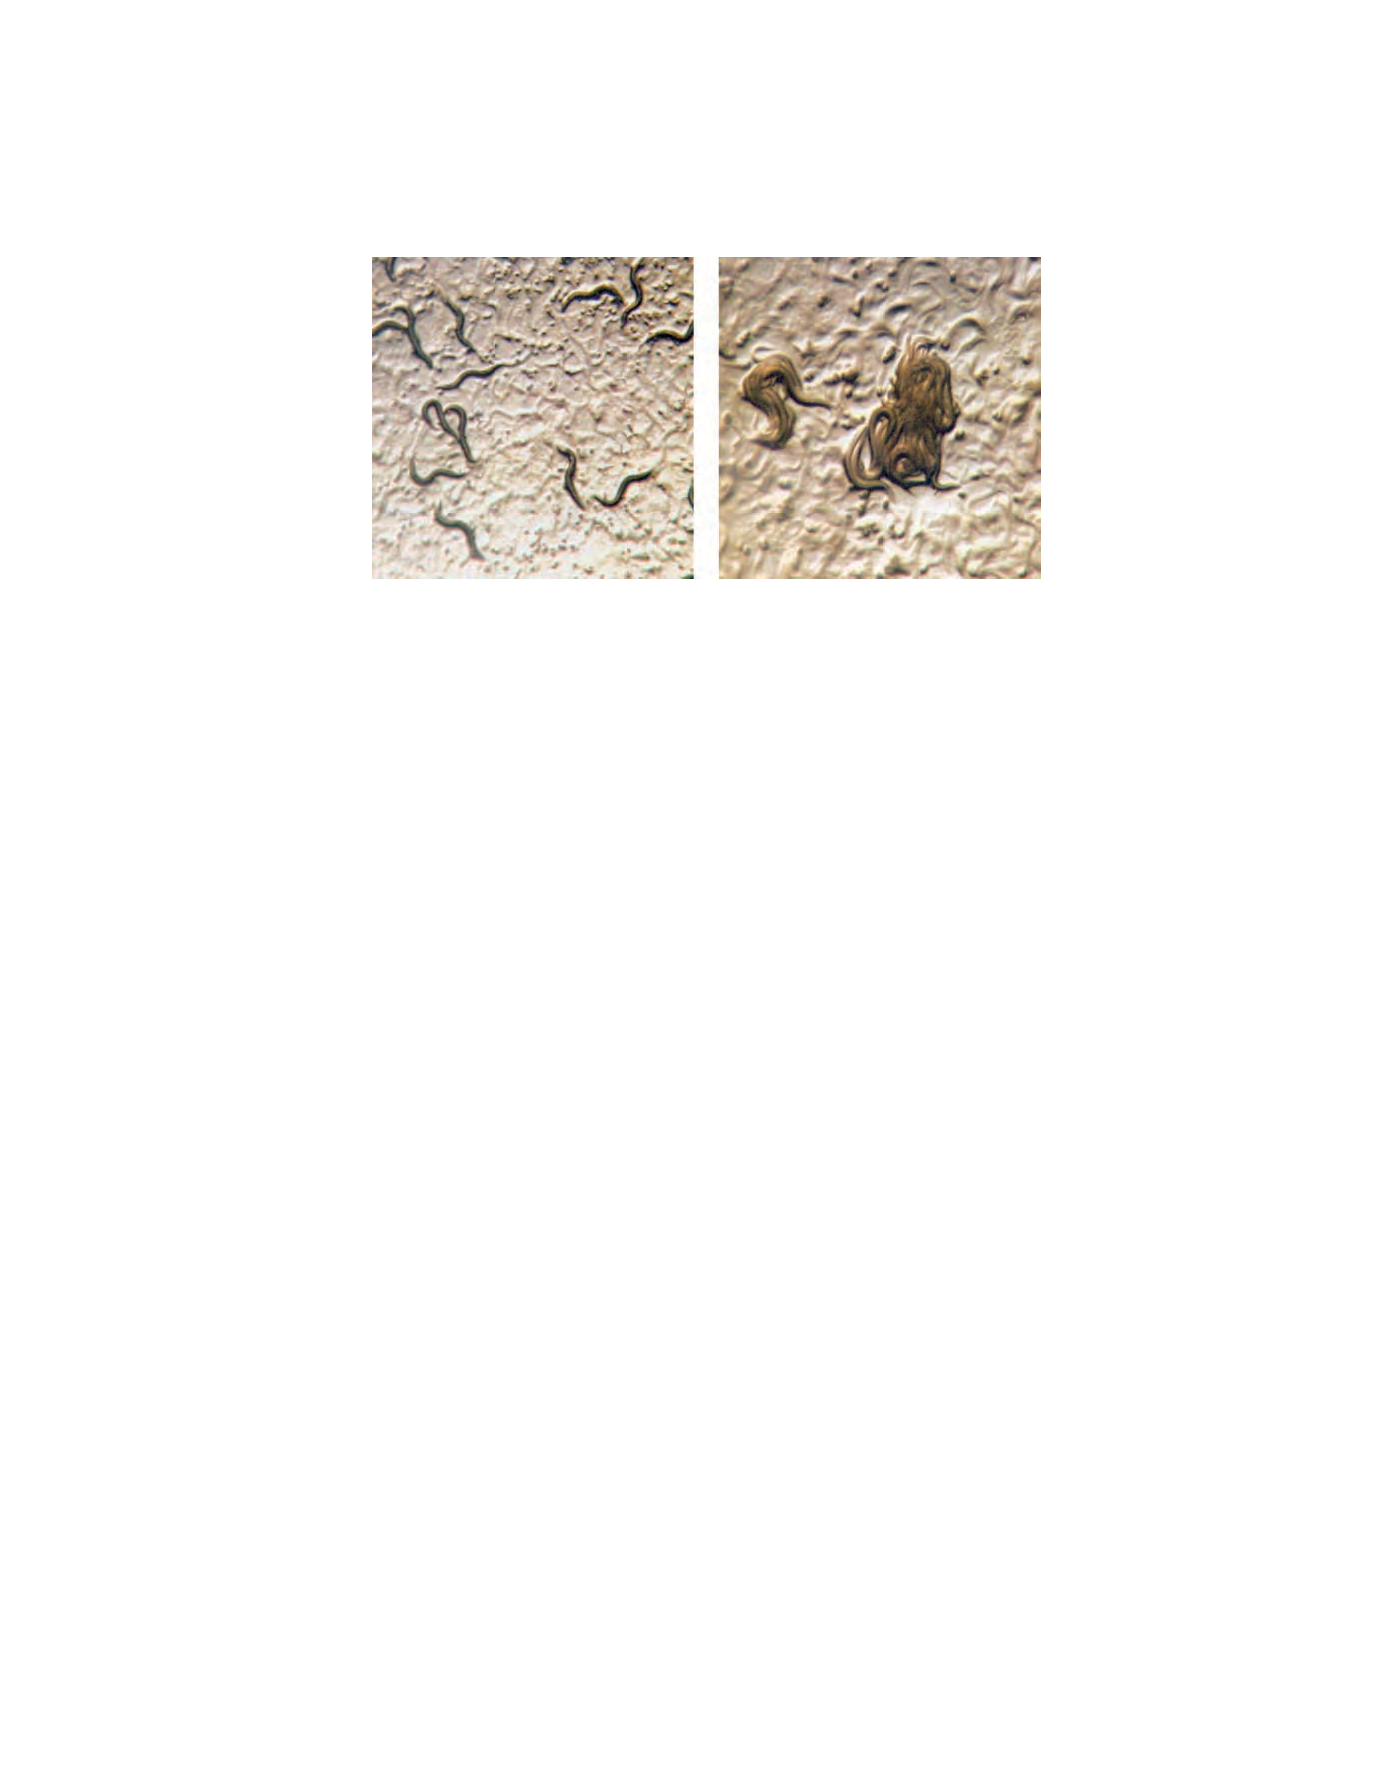
\includegraphics[width=0.7\linewidth]{chap02/fig_2_15}
	\caption{秀丽隐杆线虫的进食行为取决于编码神经肽受体的基因的活性水平。
		在一个菌株中,个体蠕虫在隔离状态下吃草(左),而在另一个菌株,个体聚集在一起觅食。
		这种差异可以通过神经肽受体基因中的单个氨基酸取代来解释\cite{de1998natural}。}
	\label{fig:2_15}
\end{figure}


群居蠕虫和独居蠕虫之间的差异是由单个基因中的单个氨基酸取代引起的,该基因是参与神经元间信号传导的一大基因家族的成员。
该基因\textit{神经肽受体}-1 编码神经肽受体。
长期以来,神经肽因其在跨神经元网络协调行为方面的作用而受到赞赏。
例如,海蜗牛的神经肽激素会刺激与单一行为(产卵)相关的一组复杂的运动和行为模式。
哺乳动物神经肽与摄食行为、睡眠、疼痛和许多其他行为和生理过程有关。
改变社会行为的神经肽受体突变的存在表明,这种信号分子对于产生行为和产生个体之间的差异都很重要。


神经肽受体也与哺乳动物社会行为的调节有关。
神经肽催产素和加压素刺激哺乳动物的亲和行为,例如配对结合和父母与后代的结合。
在小鼠中,社会认知需要催产素,即识别熟悉个体的能力。
催产素和加压素已在草原田鼠中进行了深入研究,草原田鼠是一种长期成对抚养幼崽的啮齿动物。
雌性草原田鼠在交配过程中大脑中释放的催产素会刺激配对关系的形成。
同样,雄性草原田鼠在交配过程中大脑中释放的加压素会刺激配对关系的形成和父系行为。


配对结合的程度在哺乳动物物种之间有很大差异。
雄性草原田鼠与雌性形成长期的配偶关系,帮助它们抚养后代,被描述为一夫一妻制,但密切相关的雄性山地田鼠繁殖广泛,不参与父系行为。
这些物种中雄性行为的差异与大脑中\textit{血管加压素受体}表达的差异相关。
在草原田鼠中,\textit{血管加压素受体}在特定大脑区域(腹侧苍白球)中以高水平表达(图~\ref{fig:2_16})。 
在山地田鼠中,该区域的水平要低得多,尽管其他大脑区域的水平很高。


\begin{figure}[htbp]
	\centering
	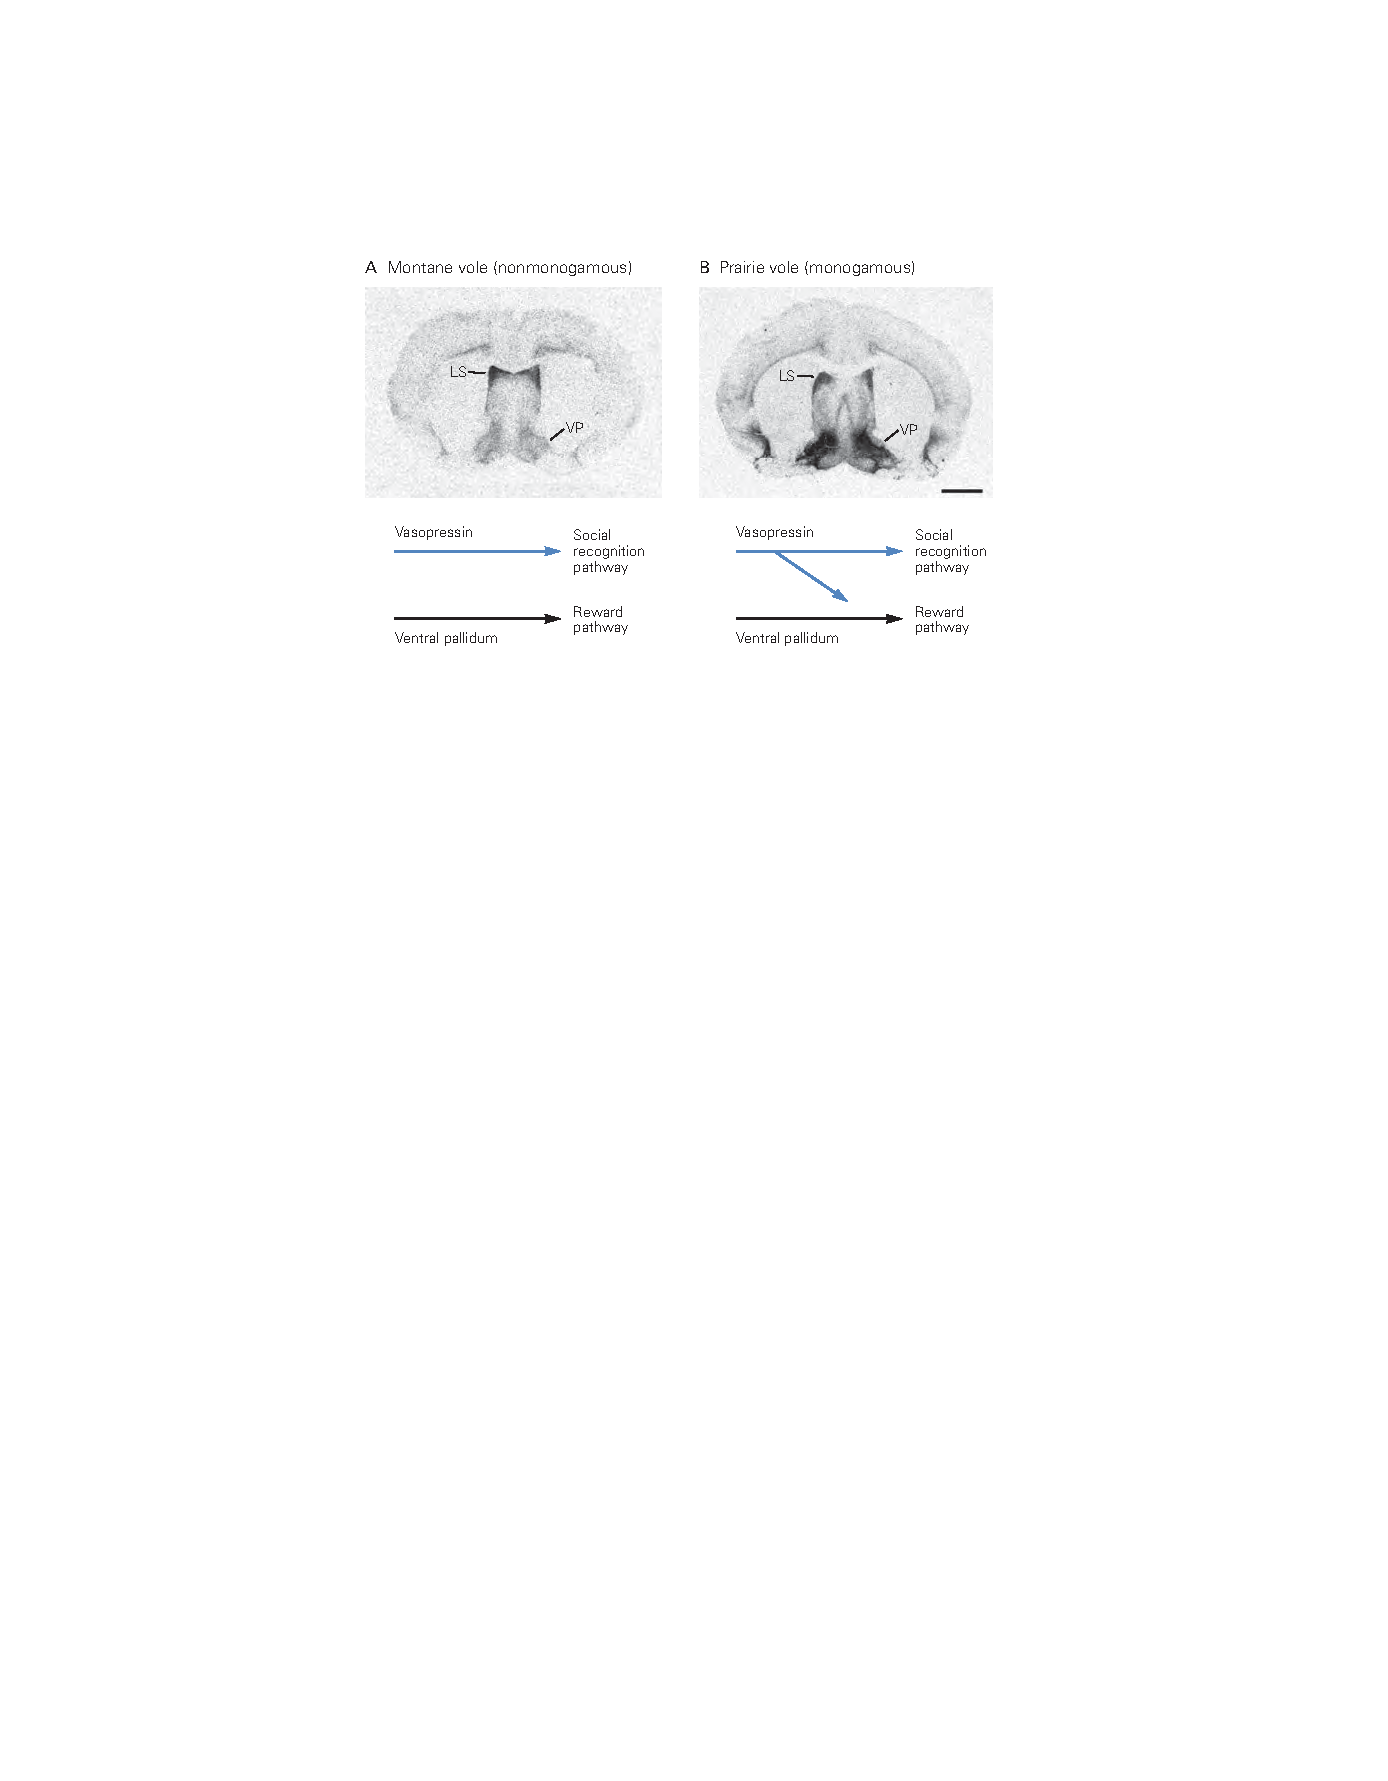
\includegraphics[width=0.72\linewidth]{chap02/fig_2_16}
	\caption{\textit{血管加压素受体}在两种亲缘关系密切的啮齿动物中的分布\cite{young2001cellular}。
		\textbf{A.} 受体在山地田鼠的\textit{外侧隔核}中表达较高,但在\textit{腹侧苍白球}中表达较低,这不会形成配对键。
		\textbf{B.} 在一夫一妻制草原田鼠的\textit{腹侧苍白球}中表达很高。
		受体在\textit{腹侧苍白球}中的表达使\textit{加压素}将\textit{社会认知通路}与\textit{奖赏通路}联系起来。}
	\label{fig:2_16}
\end{figure}


催产素和加压素及其受体的重要性已通过小鼠反向遗传研究得到证实和扩展,这比田鼠更容易进行遗传操作。
将草原田鼠的\textit{血管加压素受体}基因引入行为更像山地田鼠的雄性小鼠,增加了\textit{血管加压素受体}在腹侧苍白球中的表达,并增加了雄性小鼠对雌性的亲和行为。
因此,物种之间加压素受体表达模式的差异可能导致社会行为的差异。


对不同啮齿动物中加压素受体的分析提供了对基因和行为在进化过程中发生变化的机制的深入了解。
因此,腹侧前脑\textit{血管加压素受体}表达模式的进化变化改变了神经回路的活动,将腹侧前脑的功能与交配激活的加压素分泌神经元的功能联系起来。
结果,社会行为发生了改变。


催产素和后叶加压素在人类社会行为中的重要性尚不清楚,但配对和幼崽饲养在哺乳动物物种中的核心作用表明这些分子可能也在我们物种中发挥作用。



\section{人类遗传综合症的研究为社会行为的基础提供了初步见解}

\subsection{人类脑部疾病是基因与环境相互作用的结果}

在人类中发现的第一个神经系统疾病基因清楚地说明了基因和环境在决定认知和行为表型方面的相互作用。
\textit{苯丙酮尿症}于 1934 年由挪威的\textit{阿斯比约恩$\cdot$佛林}描述,影响 1 万 5 千名儿童中的一名,并导致认知功能严重受损。


患有这种疾病的儿童有两个编码苯丙氨酸羟化酶的\textit{苯丙酮尿症}基因的异常拷贝,苯丙氨酸羟化酶是一种将氨基酸苯丙氨酸转化为酪氨酸的酶。
该突变是隐性的,杂合子携带者个体没有任何症状。
该基因的两个拷贝都缺乏正常功能的儿童会从膳食蛋白质中积累高血浓度的苯丙氨酸,这反过来会导致产生干扰神经元功能的有毒代谢物。
苯丙氨酸对大脑产生不利影响的具体生化过程仍不清楚。


\textit{苯丙酮尿症}表型(智力障碍)是基因型(纯合子 \textit{苯丙酮尿症基因}突变)和环境(饮食)相互作用的结果。
因此,\textit{苯丙酮尿症}的治疗简单有效:可以通过低蛋白饮食来预防发育迟缓。
\textit{苯丙酮尿症}基因功能的分子和遗传分析已使受影响个体的生活得到显著改善。
自 1960 年代初以来,美国对新生儿\textit{苯丙酮尿症}进行了强制性检测。
在疾病出现之前识别患有遗传疾病的儿童并改变他们的饮食可以预防该疾病的许多方面。


本书后面的章节描述了很多单基因特征的例子,例如\textit{苯丙酮尿症},这些特征导致了对大脑功能和功能障碍的深入了解。
这些研究中出现了某些主题。
例如,许多罕见的神经退行性疾病,如亨廷顿病和脊髓小脑性共济失调,是由蛋白质中谷氨酸残基的病理性显性扩张引起的。
这些多聚谷氨酰胺重复障碍的发现突出了未折叠和聚集的蛋白质对大脑的危险。
癫痫发作可由离子通道中的各种突变引起的发现导致人们认识到这些疾病主要是神经元兴奋性障碍。



\subsection{罕见的神经发育综合症为社会行为、知觉和认知的生物学提供了见解}

在儿童时期表现出来的神经和发育障碍已经阐明了遗传学在人类大脑功能中的重要性和复杂性。
基因影响特定认知和行为回路的早期证据来自对称为\textit{威廉综合症}的罕见遗传病症的研究。
患有这种疾病的人通常表现出正常的语言和极端的社交能力;
在发育早期,他们缺乏儿童通常在陌生人面前表现出的沉默寡言。
同时,他们在空间处理方面严重受损,表现出整体智力障碍,并且焦虑率非常高(但很少有社交焦虑症)。


与孤独症谱系障碍等疾病相比,\textit{威廉综合症}的损伤模式表明,语言和社交技能可以与其他一些大脑功能区分开来。
与语言有关的大脑区域在孤独症儿童中受损,但在\textit{威廉综合症}中活跃或加重。
相比之下,\textit{威廉综合症}的一般智力和空间智力受损程度超过所有孤独症谱系障碍儿童的大约一半。


\textit{威廉综合症}是由染色体区域\textit{第7号染色体1区1带2亚带3次亚带}的杂合缺失引起的,通常包含约 1.5 Mb 和 27 个基因。
对该缺陷最简单的解释是,区间内基因的表达水平降低,因为该区域每个基因只有一个拷贝,而不是两个拷贝。
影响社会交流和空间处理的区间中的精确基因尚不清楚,但由于它们有可能提供对人类行为的遗传调控的洞察力,因此引起了极大的兴趣。


孤独症谱系障碍研究的最新发现进一步强调了遗传变异与社会和智力功能之间的复杂关系,这首先是由\textit{威廉综合症}阐明的。
大约在过去十年内,基因组技术的进步使高通量方法能够筛选基因组中染色体结构的变异,并且分辨率比光学显微镜高得多(见方框~\ref{box:2_1})。
2007 年和 2008 年的开创性研究表明,患有孤独症谱系障碍的个体比未受影响的个体更常携带新的(从头)拷贝数变异。
这些发现导致了一些特定基因组间隔的首次发现,这些间隔导致了该综合症的常见形式(即没有综合症特征证据的孤独症谱系障碍,也称为特发性或非综合症性孤独症谱系障碍)。


2011 年,在一个非常明确的队列中同时开展两项从头拷贝数变异的大规模研究发现,\textit{威廉综合症}中删除的恰好相同区域会给个体带来孤独症谱系障碍的重大风险。
然而,在这些情况下,是罕见的重复(该区域的一个多余副本),而不是缺失,大大增加了社会残疾的风险。
这些发现,即同一组基因的损失和获得可能导致截然不同的社会表型(虽然两者通常都会导致智力障碍),进一步支持认知和行为功能领域是可分离的但可能共享重要分子机制的观点。


\textit{脆性X综合症}是另一种儿童神经发育障碍,可以深入了解认知功能的遗传学;
与\textit{威廉综合症}不同,它已被映射到 X 染色体上的单个基因。
\textit{脆性X综合症}的表现各不相同。
患儿可有智力障碍、社会认知差、社交焦虑高、行为重复;
大约 30\% 的\textit{脆性X综合症}男孩符合孤独症谱系障碍的诊断标准。
\textit{脆性X综合症}还与更广泛的特征相关,包括身体特征,例如拉长的脸和突出的耳朵。


\textit{脆性X综合症}已被证明是由减少称为\textit{脆性X智力迟钝蛋白}的基因表达的突变引起的。
因为该基因落在 X 染色体上,当男性的一个拷贝发生突变时,男性将失去该基因的所有表达。
\textit{脆性X智力迟钝蛋白}蛋白在神经元中调节\textit{信使核糖核酸}向蛋白质的翻译,这一过程本身受神经元活动调节。
神经元中受调节的翻译是学习所需的突触可塑性的重要组成部分。
因此,翻译水平上的脆弱 X 缺陷会级联起来影响神经元功能、学习和高层认知过程。
有趣的是,大部分与孤独症谱系障碍和精神分裂症风险增加相关的其他基因都受\textit{脆性X智力迟钝蛋白}蛋白调节。


另一种遗传基础广为人知的孟德尔疾病是\textit{雷特综合症}(在第~\ref{chap:chap62}~章中详细讨论)。
\textit{雷特综合症}是一种 X 连锁的进行性神经发育障碍,是女性智力障碍的最常见原因之一。
这种疾病几乎总是局限于女性,因为典型的\textit{雷特}突变在发育中的男性胚胎中通常是致命的,而男性胚胎只有一条 X 染色体。
受影响的女孩通常会发育到 6 到 18 个月大,这时她们无法学会说话,智力功能退化,并且表现出强迫性、不受控制的拧手而不是有目的的手部运动。
此外,患有\textit{雷特综合症}的女孩通常会表现出一段时间的社交互动明显受损,这可能与孤独症谱系障碍无法区分,尽管人们认为社交功能在以后的生活中很大程度上得到了保留。
\textit{胡达$\cdot$佐格比}和她的同事发现,这种综合症的主要原因是甲基 CpG 结合蛋白 2(MeCP2)基因的突变。
\textit{脱氧核糖核酸}中特定 CpG 序列的甲基化会改变附近基因的表达,而 MeCP2 的一项既定功能是它结合甲基化\textit{脱氧核糖核酸}作为调节\textit{信使核糖核酸}转录过程的一部分。


罕见综合症还提供了一些对精神分裂症遗传底物的初步见解(第~\ref{chap:chap60}~章)。
例如,正如\textit{罗伯托$\cdot$什普林茨恩}及其同事在 1978 年首次描述的那样,22q11 染色体缺失会导致广泛的身体和行为症状,包括精神病,现在通常被称为\textit{腭心面综合症}、\textit{迪格奥尔格综合症}或 22q11 缺失综合症。
由于与相同缺失相关的表型范围极其广泛,\textit{什普林茨恩}的最初描述遭到了一些怀疑。
现在人们普遍认为,22q11 缺失是与精神分裂症和儿童期发病的精神分裂症相关的最常见的染色体异常。
此外,已发现同一区域的染色体丢失与孤独症的个体风险有关。
迄今为止,尚未明确确定该区域内负责精神病表型的特定基因。
此外,最近来自孤独症文献的证据表明,很可能是这个区间内多个基因的组合,每个基因赋予相对较小的个体影响,是社会残疾表型的原因。



\section{精神疾病涉及多基因特征}

如前所述,与神经退行性疾病和精神疾病的总负担相比,单基因综合症很少见。
因此,如果罕见疾病仅占总疾病负担的一小部分,人们可能会质疑研究罕见疾病的理由。
原因是罕见的情况可以让人们深入了解更常见、更复杂的疾病形式所涉及的生物学过程。
例如,人类遗传学取得的突出成就之一是发现了导致早发性阿尔茨海默病或帕金森病的罕见基因变异。
具有这些严重罕见变异的个体代表了所有患有这些疾病的个体的一小部分,但对罕见疾病变异的鉴定揭示了在更大的患者群体中也被破坏的细胞过程,指向了一般的治疗途径。
同样,对\textit{雷特综合症}、\textit{脆性X综合症}和其他神经发育障碍背后的病理生理机制的探索已经导致了对精神综合症合理药物开发的一些初步尝试。


在本章的其余部分,我们将进一步讨论两种复杂的神经发育和精神病表型的遗传学:孤独症谱系障碍和精神分裂症。
与前面讨论的罕见孟德尔例子相比,这些疾病的常见形式的遗传学确实更加多样化、多样和异质,涉及不同个体的许多不同基因以及赋予责任的多种风险基因组合。
此外,对于这两种诊断,虽然对遗传贡献的支持是巨大的,但也有令人信服的证据表明环境因素的贡献。


理解这些疾病的进展来自快速发展的基因组技术和统计方法的结合、开放数据共享的文化以及非常大的患者队列的整合,这些患者队列提供了足够的能力来检测非常罕见的高渗透性等位基因以及携带的常见遗传变异 风险的小增量。
重要的是,最近在理解这两种综合症方面取得的成功为研究它们的生物学后果以及这些遗传风险因素所传达的分子、细胞和回路级病理生理学提供了坚实的基础。



\subsection{孤独症谱系障碍遗传学的进展突出了罕见和从头突变在神经发育障碍中的作用}

孤独症谱系障碍是一组严重程度不同的发育综合症,影响大约 2\% 至 3\% 的人口,其特征是相互社会交流障碍以及刻板兴趣和重复行为。
男性明显占优势;
平均而言,受影响的男孩是女孩的三倍。
孤独症谱系障碍的临床症状,根据定义,出现在生命的前 3 年,尽管受影响和未受影响的儿童之间高度可靠的差异通常在生命的头几个月内可以识别。


受影响的人之间存在相当大的表型变异性,导致孤独症谱系障碍的诊断分类相当广泛。
此外,受影响的个体比一般人群更容易出现癫痫发作和认知问题,并且通常在适应功能方面存在严重障碍。
然而,许多孤独症患者并没有受到如此深远的影响,并过着非常成功的生活。


孤独症具有很强的遗传成分(见图~\ref{fig:2_1}A),这很可能解释了它是首批屈服于现代基因发现工具和方法的遗传复杂神经精神综合症之一。
孤独症谱系障碍具有更广泛的意义,因为它提供了对典型人类行为的洞察力:语言、复杂智力和人际互动。
重要的是,孤独症谱系障碍中的社交沟通缺陷可以与其他领域的正常智力和典型功能共存,这一事实表明大脑在某种程度上是模块化的,具有可以独立变化的不同认知功能。


虽然孤独症谱系障碍的综合症形式只占所有病例的一小部分,但在更常见的所谓“特发性”或“非综合症”形式的障碍中的首次发现也证明了罕见突变的作用,这些突变具有巨大的生物学效应。
例如,在 2003 年,对极少数具有孤独症特征的女性 X 染色体上缺失区域的基因进行测序,导致在基因\textit{神经连接蛋白4X}中发现了罕见的功能丧失突变, 一种在兴奋性神经元中编码突触粘附分子的基因,在几个受影响的男性家庭成员中发现。
此后不久,对一个患有智力障碍和孤独症谱系障碍的大型家系进行的连锁分析表明,受影响的家庭成员都携带功能丧失型 NLGN4X 突变。


染色体结构中的从头亚显微缺失和重复可能会显著增加个体患孤独症谱系障碍的风险。
这些\textit{拷贝数变异}聚集在基因组的特定区域,确定特定的风险区间。 使用这种方法的最早报告表明,染色体 16p11.2 的新生\textit{拷贝数变异},虽然仅存在于大约 0.5\% 至 1\% 的受影响个体中,但具有很大(大于 10 倍)的孤独症谱系障碍风险。
随后的研究现在已经确定了十几个或更多具有风险的新 \textit{拷贝数变异},包括\textit{第16号染色体1区1带2亚带}、\textit{第1号染色体2区1带}、\textit{第15号染色体1区1带1亚带3次亚带}和\textit{第3号染色体2区9带};
\textit{第22号染色体1区1带}、\textit{第22号染色体1区3带}(删除基因 SHANK3)和\textit{第2号染色体1区6带}(删除基因 NXRN1)的缺失;和\textit{第7号染色体1区1带2亚带3次亚带}(\textit{威廉综合症}区域)的从头重复。


有趣的是,尽管这些对孤独症谱系障碍具有很大的风险,但对其他精神疾病(包括精神分裂症和双相情感障碍)的研究发现,许多相同的区域也会增加患这些疾病的风险。
此外,通过基因型(例如,\textit{第16号染色体1区1带2亚带}缺失和重复)确定的个体研究发现了多种相关的行为表型,从特定语言障碍到智力障碍再到精神分裂症。
这种“一对多”现象对阐明精神疾病的特定病理生理机制以及概念化从基因发现到治疗的步骤提出了重要挑战。


从头开始的罕见\textit{拷贝数变异}会增加孤独症谱系障碍和其他发育障碍的风险,这一广泛且可复制的发现立即引发了一个问题,即单个基因中的罕见从头突变是否可能带来类似的风险。
事实上,低成本、高通量\textit{脱氧核糖核酸}测序技术的发展,最初集中在基因组的编码部分,导致了被认为可能破坏受影响个体基因功能(\textit{可能的基因破坏}突变)的大量从头突变的鉴定。
这些突变在不相关的个体之间近距离反复发生,现已被用作识别孤独症谱系障碍特定风险基因的手段。


对孤独症谱系障碍新生突变的大规模研究现已确定了 100 多个相关基因,其中约 45 个达到统计显著性的最高置信水平。
这些基因具有广泛的已知功能,但分析显示参与突触形成和功能以及转录调节的基因在统计学上显著过度表达。
此外,编码\textit{核糖核酸}的风险基因数量超过预期,这些\textit{核糖核酸}是脆性 X 智力低下蛋白和/或在早期大脑发育中活跃的蛋白质的目标。



\subsection{精神分裂症基因的鉴定突出了罕见和常见风险变异的相互作用}

精神分裂症影响了大约 1\% 的年轻人,导致思维障碍和情绪退缩的模式,严重损害了生活。
它具有很强的遗传性(参见图~\ref{fig:2_1}B),并且还具有与发育中胎儿的压力相关的强大环境成分。
二战荷兰饥饿冬季饥荒后不久出生的儿童在多年后患精神分裂症的风险大大增加,而母亲在 1960 年代大流行期间怀孕期间感染风疹病毒的儿童的风险也大大增加。


基因和环境都会导致精神分裂症。
与孤独症一样,人类基因组的测序、常见变异的全基因组基因分型和\textit{拷贝数变异}检测的廉价方法的开发,以及非常大的患者队列的整合,都导致了精神分裂症遗传学的转变。
首先,与早先提到的孤独症谱系障碍的发现基本平行,到 2000 年代初期,罕见的新发\textit{拷贝数变异}开始与精神分裂症的风险有关。
一小部分病例与具有较大风险的染色体异常有关,例如,\textit{第22号染色体1区1带}的缺失。
这些染色体异常与孤独症谱系障碍相关的基因座完全或几乎重叠,但这些基因座缺失和重复的风险分布似乎并不相同。
例如,虽然\textit{第16号染色体1区1带2亚带}区域的重复和缺失都与孤独症谱系障碍和精神分裂症有关,但该区域的重复更有可能导致精神分裂症,而缺失更可能与孤独症谱系障碍和智力障碍相关。


关于精神分裂症,过去十五年来最重要的发展是常见变异全基因组关联研究的出现。
与前面描述的假设驱动的候选基因研究相反,全基因组关联依赖于同时检测基因组中每个基因的多态性。
这种无假设的方法,当与有力的队列一起使用并适当校正多重比较时,已被证明是一种高度可靠和可重复的策略,用于识别所有医学常见疾病中的常见风险等位基因。


涉及近 4 万个病例和 113,000 个对照的全基因组关联研究已经确定了 108 个精神分裂症的风险位点。 
这组中任何个体遗传变异的影响都非常适度,通常导致风险增加不到 25\%。
此外,在全基因组关联研究中测定的许多遗传多态性映射到基因组编码区段之外的区域。
因此,虽然已经确定了 108 个风险基因座,但尚不完全清楚哪些基因对应于所有这些风险变异。
在某些情况下,变异与单个基因的映射足够接近,可以合理地推断出这种关系;
在其他情况下,这仍有待确定。


与精神分裂症风险有关的基因为确定该疾病的生物学基础提供了一个起点。
例如,自 20 世纪 90 年代后期以来,有证据表明一个叫做\textit{主要组织相容性}的区域与精神分裂症风险有关。
因此,在精神分裂症队列中,\textit{主要组织相容性}区域具有人类基因组任何部分中最强的全基因组关联研究信号。
队列中的大量患者使详细研究成为可能,将\textit{主要组织相容性}区域中的这种强大的风险关联信号解析为三个不同的基因座(可能是三个不同的基因)。
在这三个基因座中,一个编码补体 C4 因子的基因对疾病风险具有强烈且明确的影响。
\textit{史蒂文$\cdot$麦卡罗}和他的同事表明,补体 C4 基因座代表\textit{拷贝数变异}的自然病例,健康个体在他们拥有的基因拷贝数方面存在很大差异,并且 C4A 等位基因的表达水平与精神分裂症风险的增加相关。
随后的后续研究表明,敲除 C4 基因的小鼠在发育过程中存在突触修剪缺陷,这表明人类 C4A 过量可能导致突触修剪过度的假设,这一过程长期以来一直受到精神分裂症文献的关注。


这一发现代表了将基因组学与增加疾病风险的可能生物学机制联系起来的能力的重要证明。
即便如此,具有最高风险 C4 单倍型且没有精神分裂症家族史的个体会由于该等位基因而平均受影响的几率从 1\% 增加到大约 1.3\%。
为了获得规模感,一级亲属患有精神分裂症会导致患病风险增加约 10 倍。
这一充满希望的开端及其局限性反映了遗传学家和神经生物学家在从成功的常见变异基因发现转向详细阐述导致人类病理学的特定机制方面所面临的挑战。


除了确定许多特定的风险位点外,精神分裂症的\textit{全基因组关联研究}还反复发现许多常见等位基因的小个体效应加起来会增加风险。
这些结果为总体研究基因型表型关系提供了一个额外的、强大的途径。
事实上,已经清楚的是,个体携带的风险等位基因的数量会对患这种疾病的风险产生重大(和累加)影响。
例如,那些在所谓的多基因风险评分(与个人携带的加性遗传风险总量相关的汇总统计数据)中处于最高十分位的人,与一般人群相比,风险增加了 8 到 20 倍。
尽管累积效应的生物学特性尚不清楚,但该观察结果为研究与疾病轨迹和治疗反应相关的一系列有趣问题奠定了基础,并且几乎肯定会重振结合神经影像学和基因组学的研究。
后一种类型的调查,类似于常见变异发现的早期努力,由于研究选定的、生物学上合理的候选基因的固有局限性,可靠性较差。


最后,类似于孤独症谱系障碍所采用的高通量测序方法,也开始在精神分裂症中产生结果。
具体来说,寻找稀有和从头风险等位基因的外显子组测序已经取得了一些成功。
然而,与孤独症谱系障碍相比,此类研究需要更大的队列来确定\textit{可能的基因破坏}突变的统计学显著风险,这表明这些类型变异的总体影响大小在精神分裂症中可能要小得多。
迄今为止,这些调查已经确定了一些风险基因并涉及关键的神经生物学途径。
特别是,最近的外显子组研究指出了\textit{活性调节的细胞骨架}复合体中分子的重要性,以及包含\textit{组蛋白H3赖氨酸4特异性甲基转移酶}的基因组结构域,与精神分裂症发病机制相关。



\section{神经精神疾病遗传基础的观点}

基因影响行为的许多方面。
人类双胞胎在人格特征和精神疾病方面有着显著的相似之处,即使是分开抚养的双胞胎也是如此。 
可以培育具有特定、稳定行为特征的家畜和实验室动物;
并且越来越多地发现了广泛的遗传变异对神经发育和精神疾病的贡献。


一系列同时的进步开创了一个理解基因、大脑和行为之间关系的绝佳机会的时代。
可用于操作和研究模型系统的设备已经发生了革命性的变化。
与此同时,在确定人类神经精神疾病的遗传风险因素方面也取得了长足的进步。
尽管该领域在此过程中仍处于早期阶段,但已经出现了成功发现基因及其应用于深入生物学理解的价值的多个例子。


最近对神经发育和精神疾病的遗传学研究的许多惊人发现之一是跨越广泛诊断边界的遗传风险重叠。 
虽然生物学不遵循分类诊断标准可能并不令人惊讶,但考虑该领域如何追踪这些影响并得出新的治疗策略仍然是一个巨大的概念挑战。


此外,值得注意的是,对于许多其他尚未看到先前提到进展类型的精神疾病,计算方法很简单:
更大的投资和更大的样本量将带来更深入的洞察力。 
例如,最近对\textit{图雷特综合症}和\textit{强迫症}新生突变的研究清楚地表明,鉴定高置信度风险基因的\textit{限速因子}是\textit{亲子三人组}测序的可用性。
同样,\textit{重度抑郁症}的\textit{全基因组关联研究}直到最近才达到足以确认具有统计学意义相关常见变异的样本量。 
这些研究包括了数十万人,并且毫不奇怪地发现了具有非常小个体影响的风险等位基因。


最后一点强调了一种想法,即一种尺寸并不适合所有行为、发育和精神疾病的基因组学。 
从模型系统的研究,到罕见孟德尔疾病的阐明,再到解开导致常见疾病的常见和罕见变异,当今可用的工具和机会是前所未有的。 
未来几年应该会深入了解精神疾病和神经发育障碍的生物学,或许还有可能帮助患者及其家人的疗法。


\section{亮点}

1. \textit{脆性X综合症}、\textit{雷特综合症}和\textit{威廉综合症}等罕见遗传综合症为复杂人类行为的分子机制提供了重要见解。 
此外,虽然仍有大量工作要做,但对这些综合症的研究已经挑战了相关认知和行为缺陷是不可改变的观念,并证明了广泛的模型系统在阐明保守生物学机制方面的效用。


2. 人类基因组测序、高通量基因组分析的发展以及同步计算和方法学的进步导致对人类行为和精神疾病遗传学的理解发生了深刻变化。
包括精神分裂症和孤独症在内的几种典型疾病已经取得了显著进展,导致鉴定出数十个明确的风险基因和染色体区域。


3. 过去十年精神病学遗传学和基因组学领域的成熟揭示了测试预先指定的候选基因的脆弱性。 
这些类型的研究现在已被常见和稀有等位基因的全基因组扫描所取代。 
再加上严格的统计框架和共识统计阈值,这些正在产生高度可靠和可重复的结果。


4. 目前,累积的证据表明,各种遗传变异构成复杂行为综合症的基础,包括常见和罕见、传播和新生、种系和体细胞、序列和染色体结构变异。 
然而,这些不同类型的遗传变化的相对贡献因特定疾病而异。


5. 人类行为遗传学最新进展的一个惊人发现是具有不同症状和自然史的综合症的遗传风险重叠。 
了解相同的突变如何以及为什么会在不同个体中导致高度不同的表型结果将是未来的主要挑战。


6. 对常见精神疾病的研究结果表明遗传异质性极高。 
这一点,再加上迄今为止已确定的风险基因的生物学多效性,以及人类大脑发育的动态性和复杂性,都表明在从对风险基因的理解转向对行为的理解方面面临着重大挑战。 
同样,目前,阐明风险基因的生物学和揭示行为综合症的病理生理学之间存在重要区别。

%\section{术语表}

%\section{选读}





\chapter{神经细胞、神经回路和行为} \label{chap:chap3}

人类行为的非凡能力范围取决于与大脑相连的一系列复杂的感觉受体,大脑是一种高度灵活的神经器官,可以从感觉信号流中选择环境中和身体内环境中的事件,这些事件对人类个人来说很重要。
大脑主动组织感官信息,用于感知、行动、决策、审美和未来参考——也就是记忆。
它也明智地忽略和丢弃信息,一个人希望,并向其他大脑报告其中一些操作及其心理表现。
所有这一切都是由相互连接的神经细胞完成的。


单个神经细胞或神经元是大脑的基本信号单元。 
人脑包含大量此类细胞,大约有 860 亿个神经元,可分为至少一千种不同的类型。 
然而,这些种类繁多的神经元与其说是人类行为复杂性的一个因素,不如说是它们组织成具有精确功能的解剖回路。 
事实上,大脑的一个关键组织原则是:
由于它们相连的方式不同,具有相似特性的神经细胞可以产生不同的行为。


由于相对较少的神经系统组织原则会产生相当大的功能复杂性,因此可以通过关注神经系统的五个基本特征来深入了解神经系统如何产生行为:

1. 单个神经细胞的结构成分;

2. 神经元在自身内部和彼此之间产生信号的机制;

3. 神经细胞之间以及神经细胞与其目标(肌肉和腺体效应器)之间的连接模式;

4. 不同互联模式与不同行为类型的关系;

5. 经验如何改变神经元及其连接。


本书的各个部分都是围绕这五个主要主题组织的。 
在本章中,我们将依次介绍这些主题,概述行为的神经控制。
我们首先考虑神经元的结构和功能以及围绕和支持它们的\textit{神经胶质细胞}。
然后,我们检查单个细胞如何组织和传输信号,以及一些相互连接的神经细胞之间的信号如何产生简单的行为,即膝跳反射。
然后,我们将这些想法扩展到更复杂的行为,由更复杂和可延展的回路调节。



\section{神经系统有两类细胞}

神经系统中主要有两类细胞:\textit{神经元}和\textit{神经胶质细胞}。


\subsection{神经细胞是神经系统的信号单位}

一个典型的神经元有四个形态学上定义的区域:\textit{细胞体}、\textit{树突}、\textit{轴突}和\textit{突触前末梢}(图~\ref{fig:3_1})。 
正如我们将要看到的,每个区域在产生信号和与其他神经细胞通信方面都有不同的作用。


\begin{figure}[htbp]
	\centering
	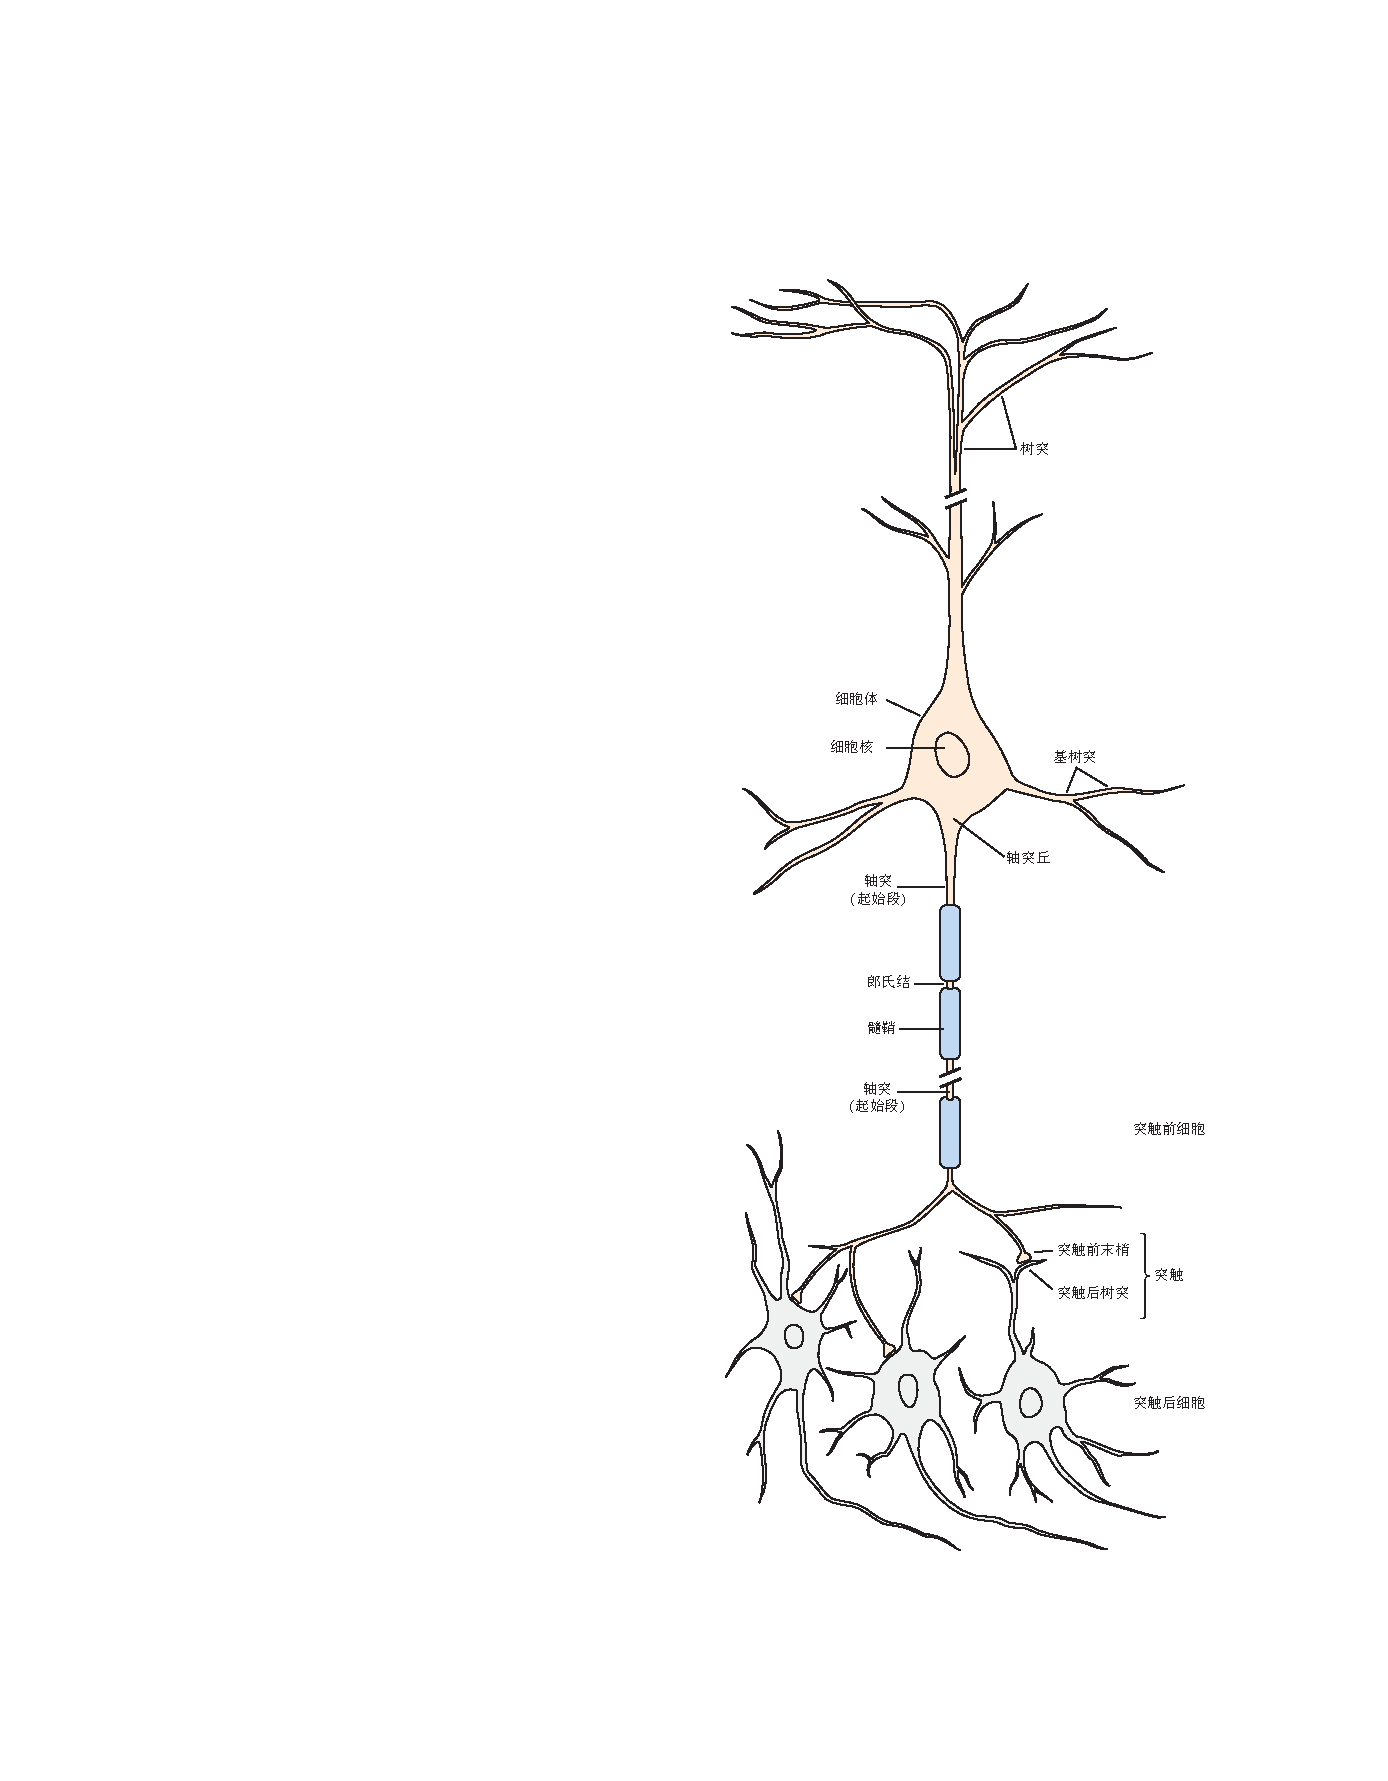
\includegraphics[width=0.5\linewidth]{chap03/fig_3_1}
	\caption{(右)神经元的结构。 
		脊椎动物神经系统中的大多数神经元有几个共同的主要特征。 
		细胞体包含细胞核,遗传信息的仓库,并产生两种类型的细胞过程:轴突和树突。 
		轴突是神经元的传递元件;
		它们的长度差异很大,有些在体内延伸超过 1 米。 
		与细胞体的直径(50 微米或更大)相比,中枢神经系统中的大多数轴突非常细(直径在 0.2 微米和 20 微米之间)。 
		许多轴突被一层脂肪\textit{髓鞘}绝缘,该鞘在称为\textit{郎氏结}的间隙处定期中断。 
		动作电位,即细胞的传导信号,在轴突的初始部分启动并传播到突触,突触是信号从一个神经元流向另一个神经元的部位。 
		突触前神经元的轴突分支将信号传递给突触后细胞。 
		单个轴突的分支可能与多达一千个突触后神经元形成突触。 
		顶端和基部树突与细胞体一起是神经元的输入元件,接收来自其他神经元的信号。}
	\label{fig:3_1}
\end{figure}


\textit{细胞体}是细胞的代谢中心。 
它包括含有细胞基因的细胞核和内质网,内质网是细胞核的延伸部分,细胞的蛋白质在这里合成。
细胞体通常产生两种过程:几个短的\textit{树突}和一个长的管状\textit{轴突}。 
树突以树状方式分支,是接收来自其他神经细胞的输入信号的主要装置。 
轴突通常在分支之前从细胞体延伸一定距离,使其能够将信号传递给许多目标神经元。
轴突可以在 0.1 毫米到 1 米的距离内传输电信号。 
这些电信号或动作电位在轴突起源附近的专门触发区域启动,称为\textit{起始段},动作电位从该区域以 1 米每秒至 100 米每秒的速度沿着轴突传播而不会失败或失真。 
沿轴突向下传播的动作电位的振幅保持恒定在 100 毫伏,因为动作电位是一种全有或全无的脉冲,它会沿着轴突定期再生(图~\ref{fig:3_2})。


\begin{figure}[htbp]
	\centering
	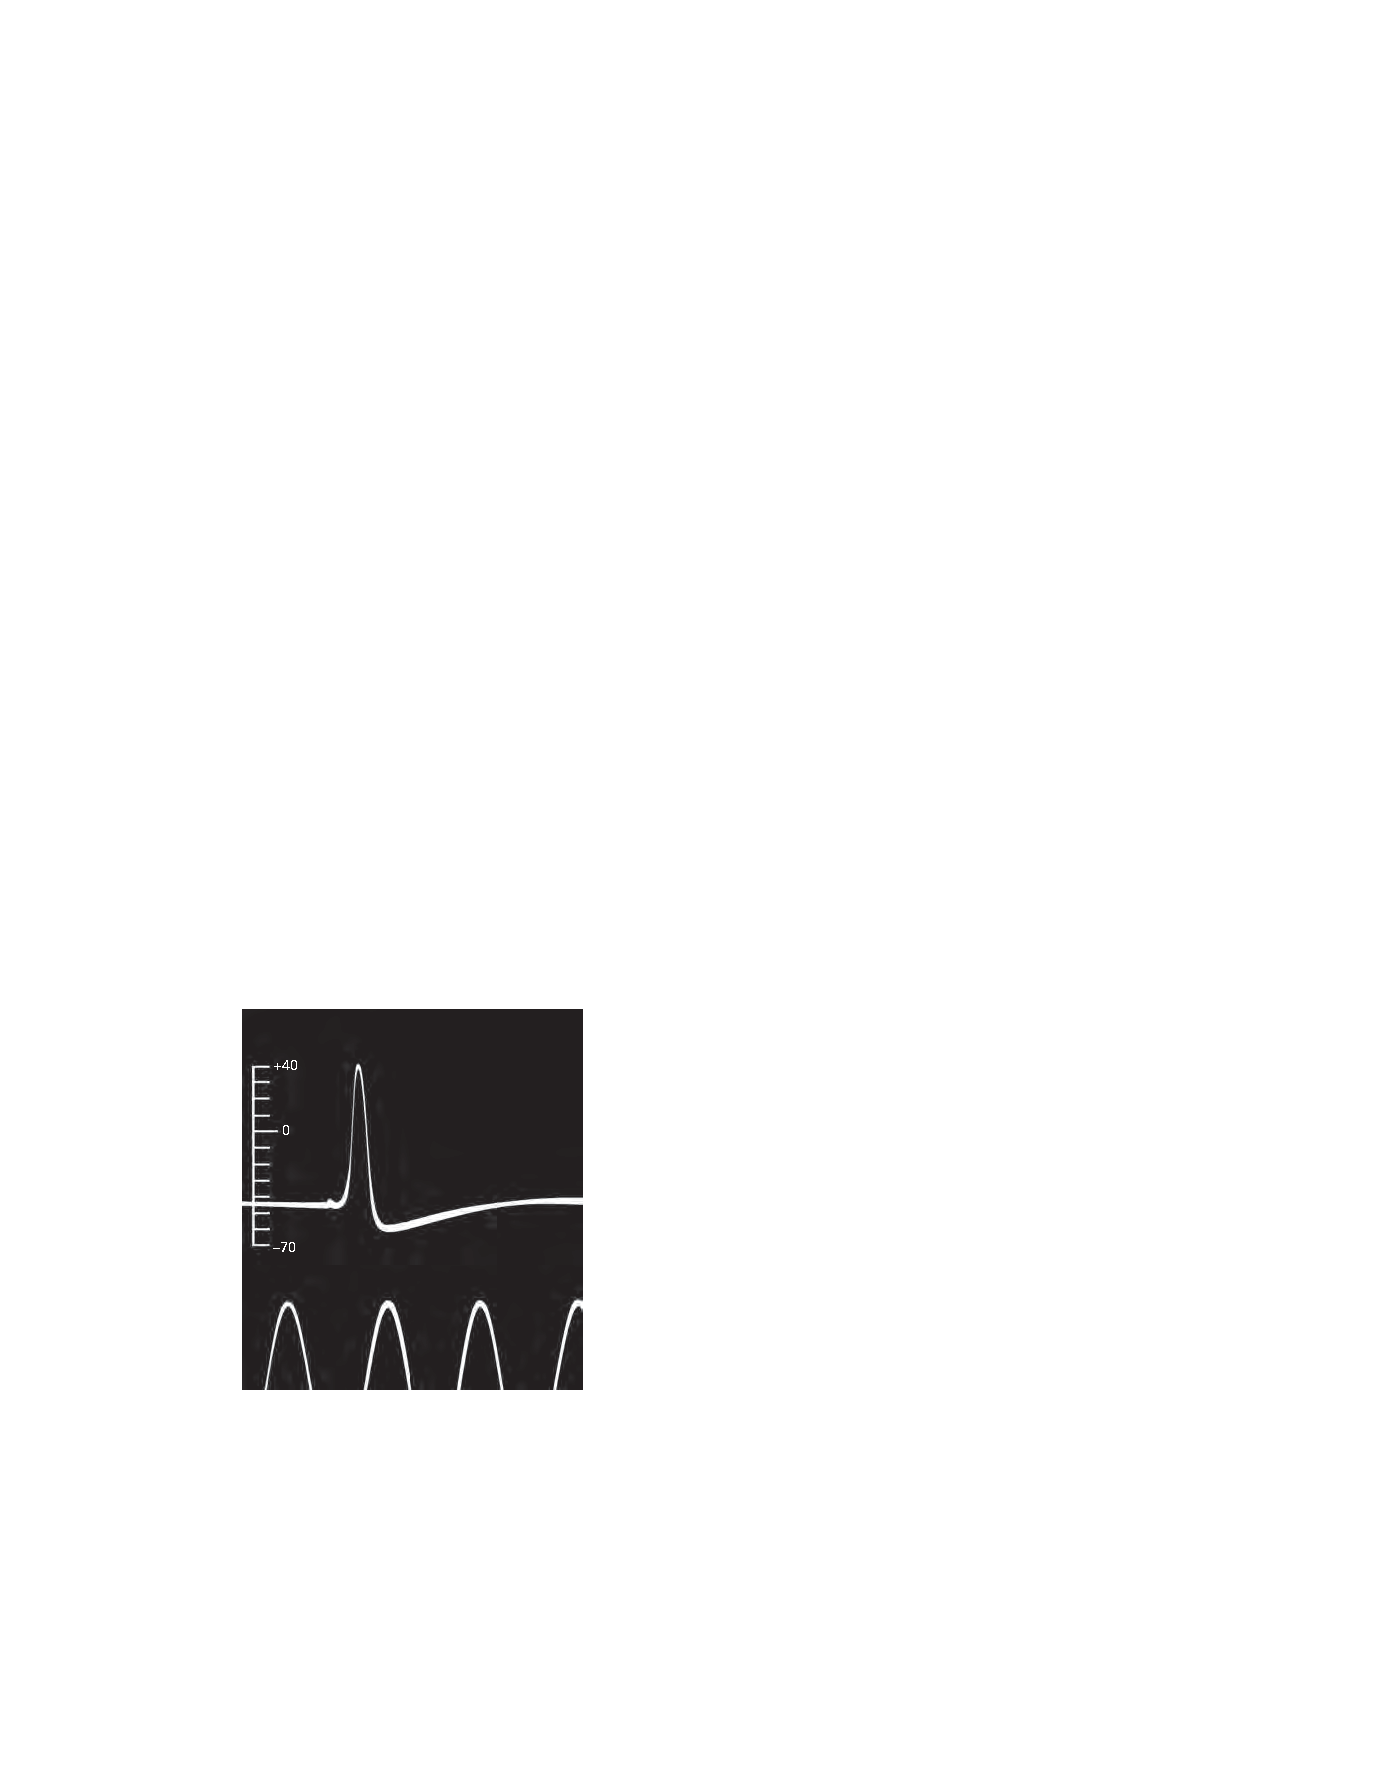
\includegraphics[width=0.5\linewidth]{chap03/fig_3_2}
	\caption{这一历史性追踪是首次公布的动作电位细胞内记录。 
		1939 年,\textit{艾伦·霍奇金}和\textit{安德鲁·赫胥黎}使用充满海水的玻璃毛细管电极从乌贼巨型轴突上记录下来。
		定时脉冲(底部)间隔 2 毫秒。 
		垂直刻度表示内部电极的电位,单位为毫伏,外面的海水被视为零电位\cite{hodgkin1939action}。}
	\label{fig:3_2}
\end{figure}


动作电位是大脑接收、分析和传递信息的信号。 
这些信号在整个神经系统中都是高度固定的,尽管它们是由环境中影响我们身体的各种事件引发的——从光到机械接触,从气味到压力波。
传递视觉信息的生理信号与传递气味信息的生理信号相同。
在这里,我们看到了大脑功能的一个关键原则:
动作电位传递的信息类型不是由信号的形式决定的,而是由信号在大脑中传播的通路决定。
因此,大脑分析和解释通过特定通路传输的传入电信号模式,进而创造我们的视觉、听觉、触觉、嗅觉和味觉。


为了提高传导动作电位的速度,大轴突被包裹在脂质物质髓磷脂的绝缘鞘中。 
鞘被\textit{郎飞结}定期中断,\textit{郎飞结}是轴突上再生动作电位的未绝缘点。
(第~\ref{chap:chap7}~章和第~\ref{chap:chap8}~章详细讨论了髓鞘形成,第~\ref{chap:chap10}~章详细讨论了动作电位。)


在接近其末端时,轴突分成细枝,这些细枝在称为突触的特殊通讯区域与其他神经元联系。
传递信号的神经细胞称为突触前细胞;
接收信号的细胞是突触后细胞。
突触前细胞从其轴突分支的特殊扩大区域传输信号,称为突触前末梢或神经末梢。
突触前细胞和突触后细胞被一个非常狭窄的空间隔开,即突触间隙。
大多数突触前终端终止于突触后神经元的树突,但有些也终止于细胞体,或者较少见的是终止于突触后细胞轴突的起点或末端(见图~\ref{fig:3_1})。 
一些突触前神经元会激发它们的突触后靶细胞;
其他突触前神经元抑制它们的靶细胞。


神经元学说(第~\ref{chap:chap1}~章)认为每个神经元都是一个离散的细胞,其细胞体具有独特的过程,并且神经元是神经系统的信号单元。
回想起来,很难体会到科学家最初提出这个基本想法时有多难接受。
与其他组织的细胞具有简单的形状并适合光学显微镜的单个视野不同,神经细胞具有复杂的形状。
树突的复杂模式和一些轴突看似无穷无尽的过程使得在这些元素之间建立关系变得极其困难。
即使在解剖学家\textit{雅各布·施莱登}和\textit{西奥多·施旺}于 1830 年代初期提出细胞理论之后——细胞是所有生命物质的结构单元的观点成为生物学的中心教条——大多数解剖学家也不接受细胞理论应用于大脑,他们认为大脑是一个连续的、网状的网状结构,由非常薄的过程组成。


神经元的连贯结构直到 19 世纪后期才变得清晰,当时 \textit{拉蒙-卡哈尔}开始使用高尔基体引入的银染法。
这种方法至今仍在使用,它有两个优点。
首先,以一种不为人知的随机方式,银溶液仅染色任何特定大脑区域中约 1\% 的细胞,这使得独立于其相邻神经元检查单个神经元成为可能。
其次,确实吸收了染色剂的神经元被完整地描绘出来,包括细胞体、轴突和完整的树突树。
染色表明神经元之间没有细胞质连续性,\textit{卡哈尔}预言性地正确地得出结论,即使在两个细胞之间的突触处也没有连续性。


\textit{拉蒙-卡哈尔}将高尔基的方法应用于许多动物和人类的胚胎神经系统。 
通过检查神经系统几乎每个区域的神经元结构,他可以描述神经细胞的类别并绘制出许多神经细胞之间的精确联系。
通过这种方式,除了神经元学说之外,\textit{拉蒙-卡哈尔}还推导出了另外两个神经组织原理,这两个原理在研究神经系统的交流方面特别有价值。


% 传播方向的极化(偏向于一边)?
其中第一个是\textit{动态极化}原理,它指出神经细胞内的电信号仅沿一个方向流动:
从神经元的突触后部位(通常是树突和细胞体)到轴突的触发区域。
从那里,动作电位沿着轴突的整个长度传播到其末端。
在迄今为止研究的大多数神经元中,电信号实际上沿着轴突向一个方向传播。


\textit{拉蒙-卡哈尔}提出的第二个原则,即\textit{连接特异性},指出神经细胞在网络形成过程中不会随机相互连接,而是在特定接触点与某些突触后靶细胞而非其他突触后靶细胞建立特定连接。
\textit{动态极化}原理和\textit{连接特异性}原理是现代细胞连接主义研究大脑方法的基础。


\textit{拉蒙-卡哈尔}也是最早意识到一种神经元与另一种神经元最具区别的特征是形状,特别是细胞体产生过程的数量。 
因此,神经元分为三大类:单极、双极和多极。


单极神经元是最简单的,因为它们只有一个初级过程,通常会产生许多分支。
一个分支作为轴突,其他分支充当接收结构(图~\ref{fig:3_3}A)。
这些细胞在无脊椎动物的神经系统中占主导地位;
在脊椎动物中,它们发生在自主神经系统中。


\begin{figure}[htbp]
	\centering
	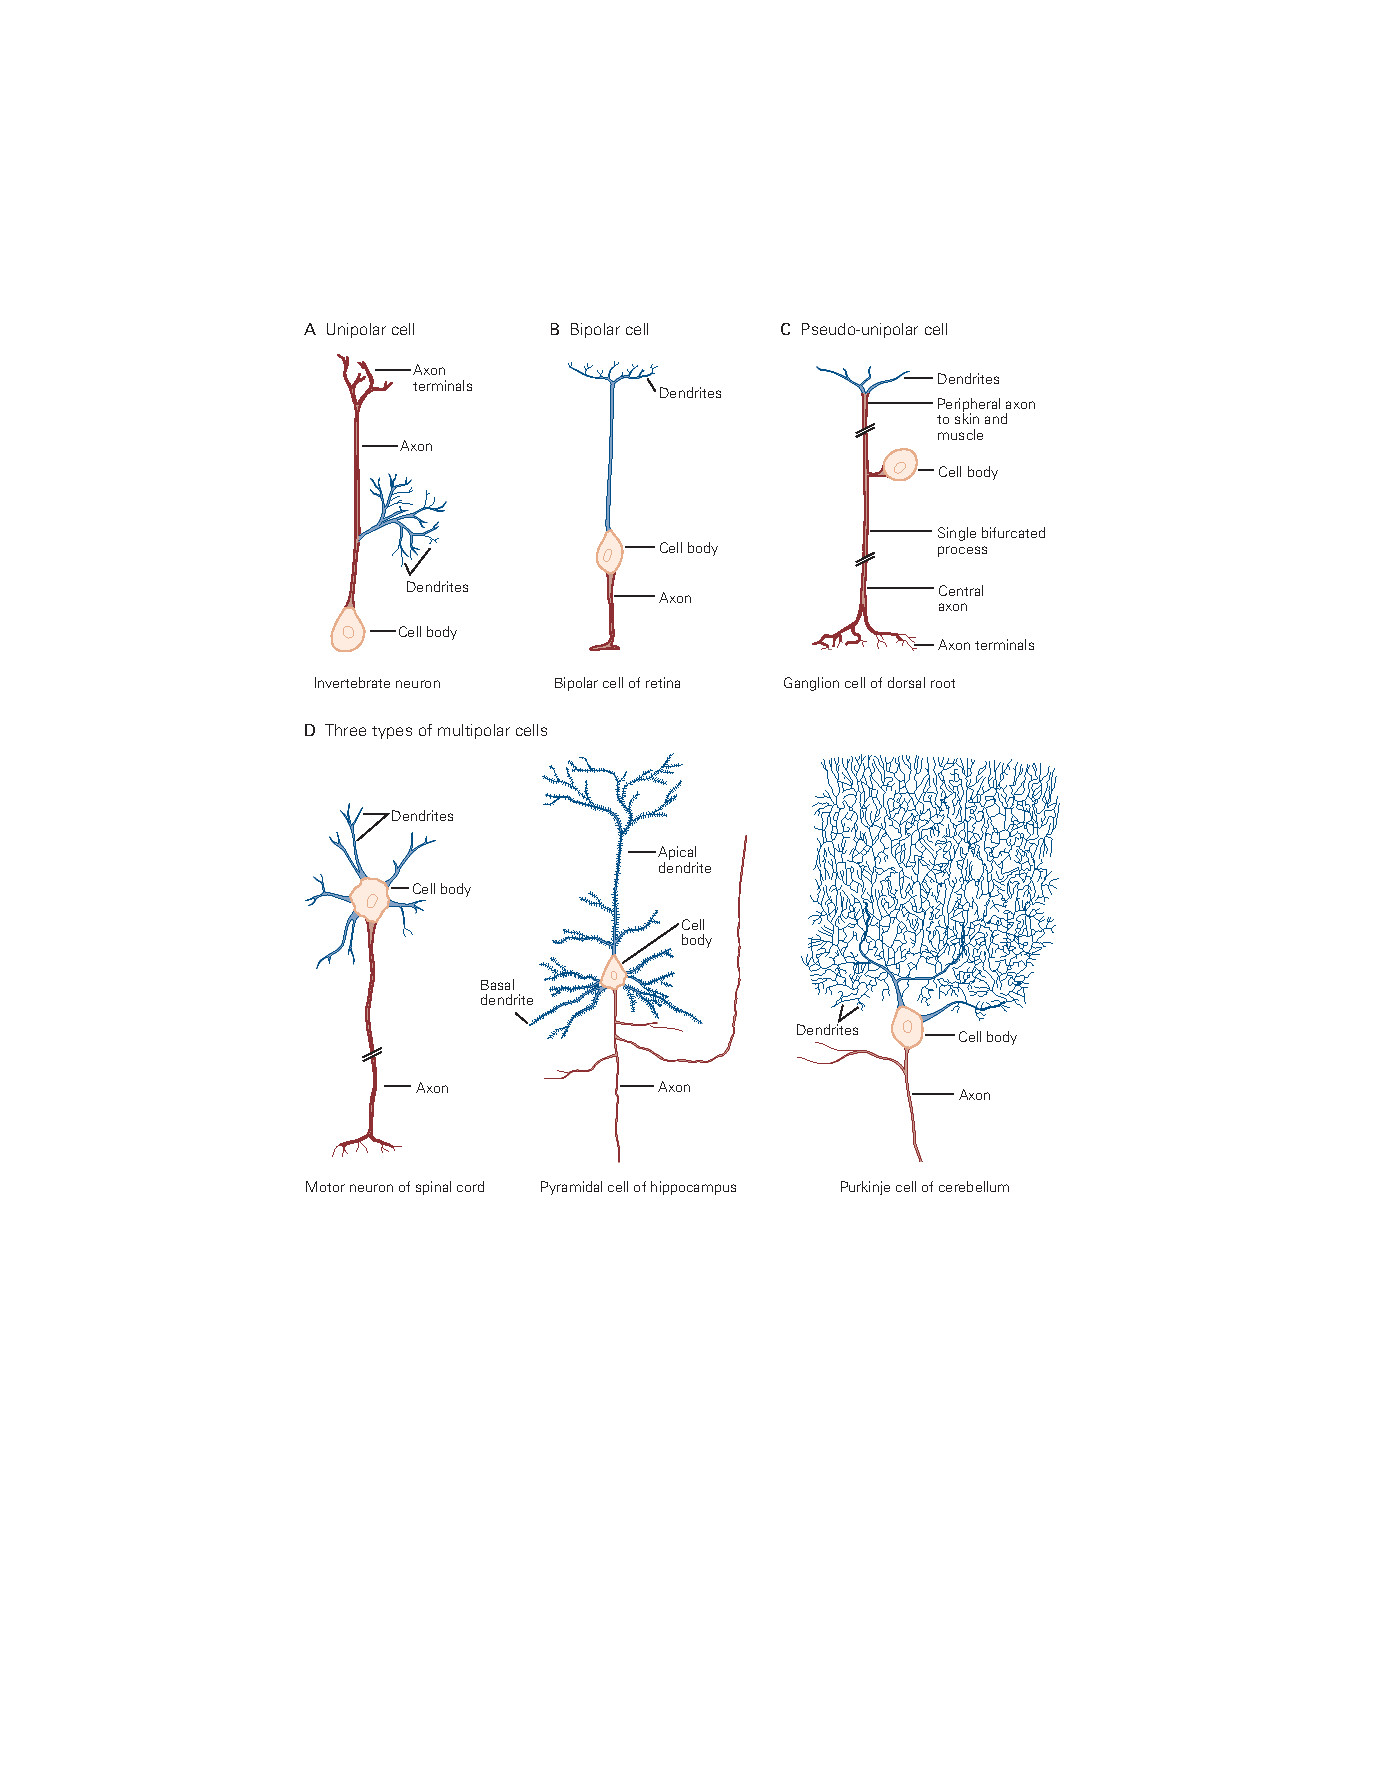
\includegraphics[width=0.9\linewidth]{chap03/fig_3_3}
	\caption{根据源自细胞体的过程的数量,神经元分为单极、双极或多极。 
		\textbf{A.} 单极细胞有一个从细胞发出的过程。
		不同的部分作为接受表面或释放终端。
		单极细胞是无脊椎动物神经系统的特征。 
		\textbf{B.} 双极细胞有两种功能专门化的过程。
		树突接收电信号,轴突将信号传递给其他细胞。
		\textbf{C.} 伪单极细胞是双极细胞的变体,将体感信息传递到脊髓。
		在发育过程中,胚胎双极细胞的两个过程融合并作为一个过程从细胞体中出现,该过程具有两个功能不同的部分。 
		两个部分都起轴突的作用;
		一个延伸到外周皮肤或肌肉,另一个延伸到中央脊髓\cite{ross2006histology}。
		\textbf{D.} 多极细胞具有单个轴突和许多树突。 
		它们是哺乳动物神经系统中最常见的神经元类型。 
		三个例子说明了这些细胞的巨大多样性。 
		脊髓运动神经元支配骨骼肌纤维。
		锥体细胞具有大致三角形的细胞体;
		树突从顶点(顶端树突)和基部(基底树突)出现。 
		锥体细胞存在于海马体和整个大脑皮层中。 
		小脑的浦肯野细胞的特征是丰富而广泛的树突状树,可容纳大量突触输入\cite{ross2006histology}。}
	\label{fig:3_3}
\end{figure}


\textit{双极神经元}有一个椭圆形的体细胞,它产生两个不同的过程:
一个树突结构接收来自其他神经元的信号,一个轴突将信息传递给中枢神经系统(图~\ref{fig:3_3}B)。
许多感觉细胞是双极的,包括\textit{视网膜双极细胞}和鼻子的嗅觉上皮细胞。
向脊髓传递触觉、压力和疼痛信号的受体神经元最初发育为双极细胞,但两个细胞过程融合成一个单一的连续结构,从细胞体的一个点出现,树突被赋予了 使它成为轴突的特化。 
在这些所谓的\textit{假单极细胞}中,一个轴突将信息从皮肤、关节和肌肉中的感觉受体传递到细胞体,而另一个轴突将此感觉信息传递到脊髓(图~\ref{fig:3_3}C)。


\textit{多极神经元}在脊椎动物的神经系统中占主导地位。 
它们通常有一个轴突和许多从细胞体周围不同点出现的树突结构(图 \ref{fig:3_3}D)。 
多极细胞的形状差异很大,尤其是轴突的长度以及树突分支的范围、尺寸和复杂性。 
通常,分支的程度与其他神经元与其进行的突触接触的数量相关。 
一个树突数量相对较少的脊髓运动神经元接受大约 1 万个接触,其中 1 千个在细胞体上,9 千个在树突上。
在小脑的\textit{浦肯野细胞}中,树突树更大更茂密,接受多达一百万次接触!


神经细胞也分为三个主要功能类别:
感觉神经元、运动神经元和中间神经元。 
\textit{感觉神经元}将信息从身体的外围传感器传送到神经系统,以达到感知和运动协调的目的。 
一些\textit{初级感觉神经元}称为\textit{传入神经元},这两个术语可以互换使用。 
术语\textit{传入}(传向中枢神经系统)适用于从外围到达中枢神经系统的所有信息,无论该信息是否导致感觉。
术语\textit{感觉}是指那些将信息从感觉上皮细胞、关节感觉受体或肌肉传递到中枢神经系统的传入神经元,但该概念已扩展到包括初级和次级皮层区域中的神经元,这些神经元对变化做出反应 感觉特征,例如物体在空间中的位移、声音频率的变化或头部的角旋转(通过耳朵中的前庭器官),甚至像面部这样复杂的东西。


\textit{传出}一词适用于从中枢神经系统向运动器官传递的所有信息,无论这些信息是否导致行动。
\textit{运动神经元}将命令从大脑或脊髓传递到肌肉和腺体(传出信息)。 
运动神经元(或运动神经元)的传统定义是激发肌肉的神经元,但运动神经元的名称现在包括不直接支配肌肉但间接命令动作的其他神经元。
运动神经元和感觉神经元的一个有用特征是它们对神经系统外事物的时间保真度。 
它们的活动跟上外部刺激和身体肌肉组织施加动力的变化。 
感觉神经元为大脑提供数据,而运动神经元将观念转化为实践。 
它们共同构成了我们与世界的连接。


\textit{中间神经元}包含最多的功能类别,并细分为两类:\textit{中继中间神经元}和\textit{局部中间神经元}。
中继中间神经元或投射中间神经元具有长轴突,可在相当长的距离内将信号从一个大脑区域传送到另一个大脑区域。
局部中间神经元的轴突较短,因为它们与局部回路中附近的神经元形成连接。
由于几乎每个神经元都可以被视为中间神经元,因此该术语通常用于区分投射到局部回路中另一个神经元的神经元和投射到单独神经结构的神经元。
该术语有时也用作抑制性神经元的简写,特别是在皮层回路的研究中,但为了清楚起见,应在适当的时候使用\textit{抑制性中间神经元}术语。


每个功能分类可以进一步细分。 
感觉系统中间神经元可以根据它们响应的感觉刺激的类型进行分类; 
这些最初的分类可以根据位置、密度、大小以及基因表达模式进一步细分。
事实上,由于\textit{信使核糖核酸}序列分析的进步使得能够对单个神经元进行分子分析,我们对神经元复杂性的看法正在迅速发展。 
此类分析最近揭示了神经元类型的异质性比以前认为的要大得多(图~\ref{fig:3_4})。


\begin{figure}[htbp]
	\centering
	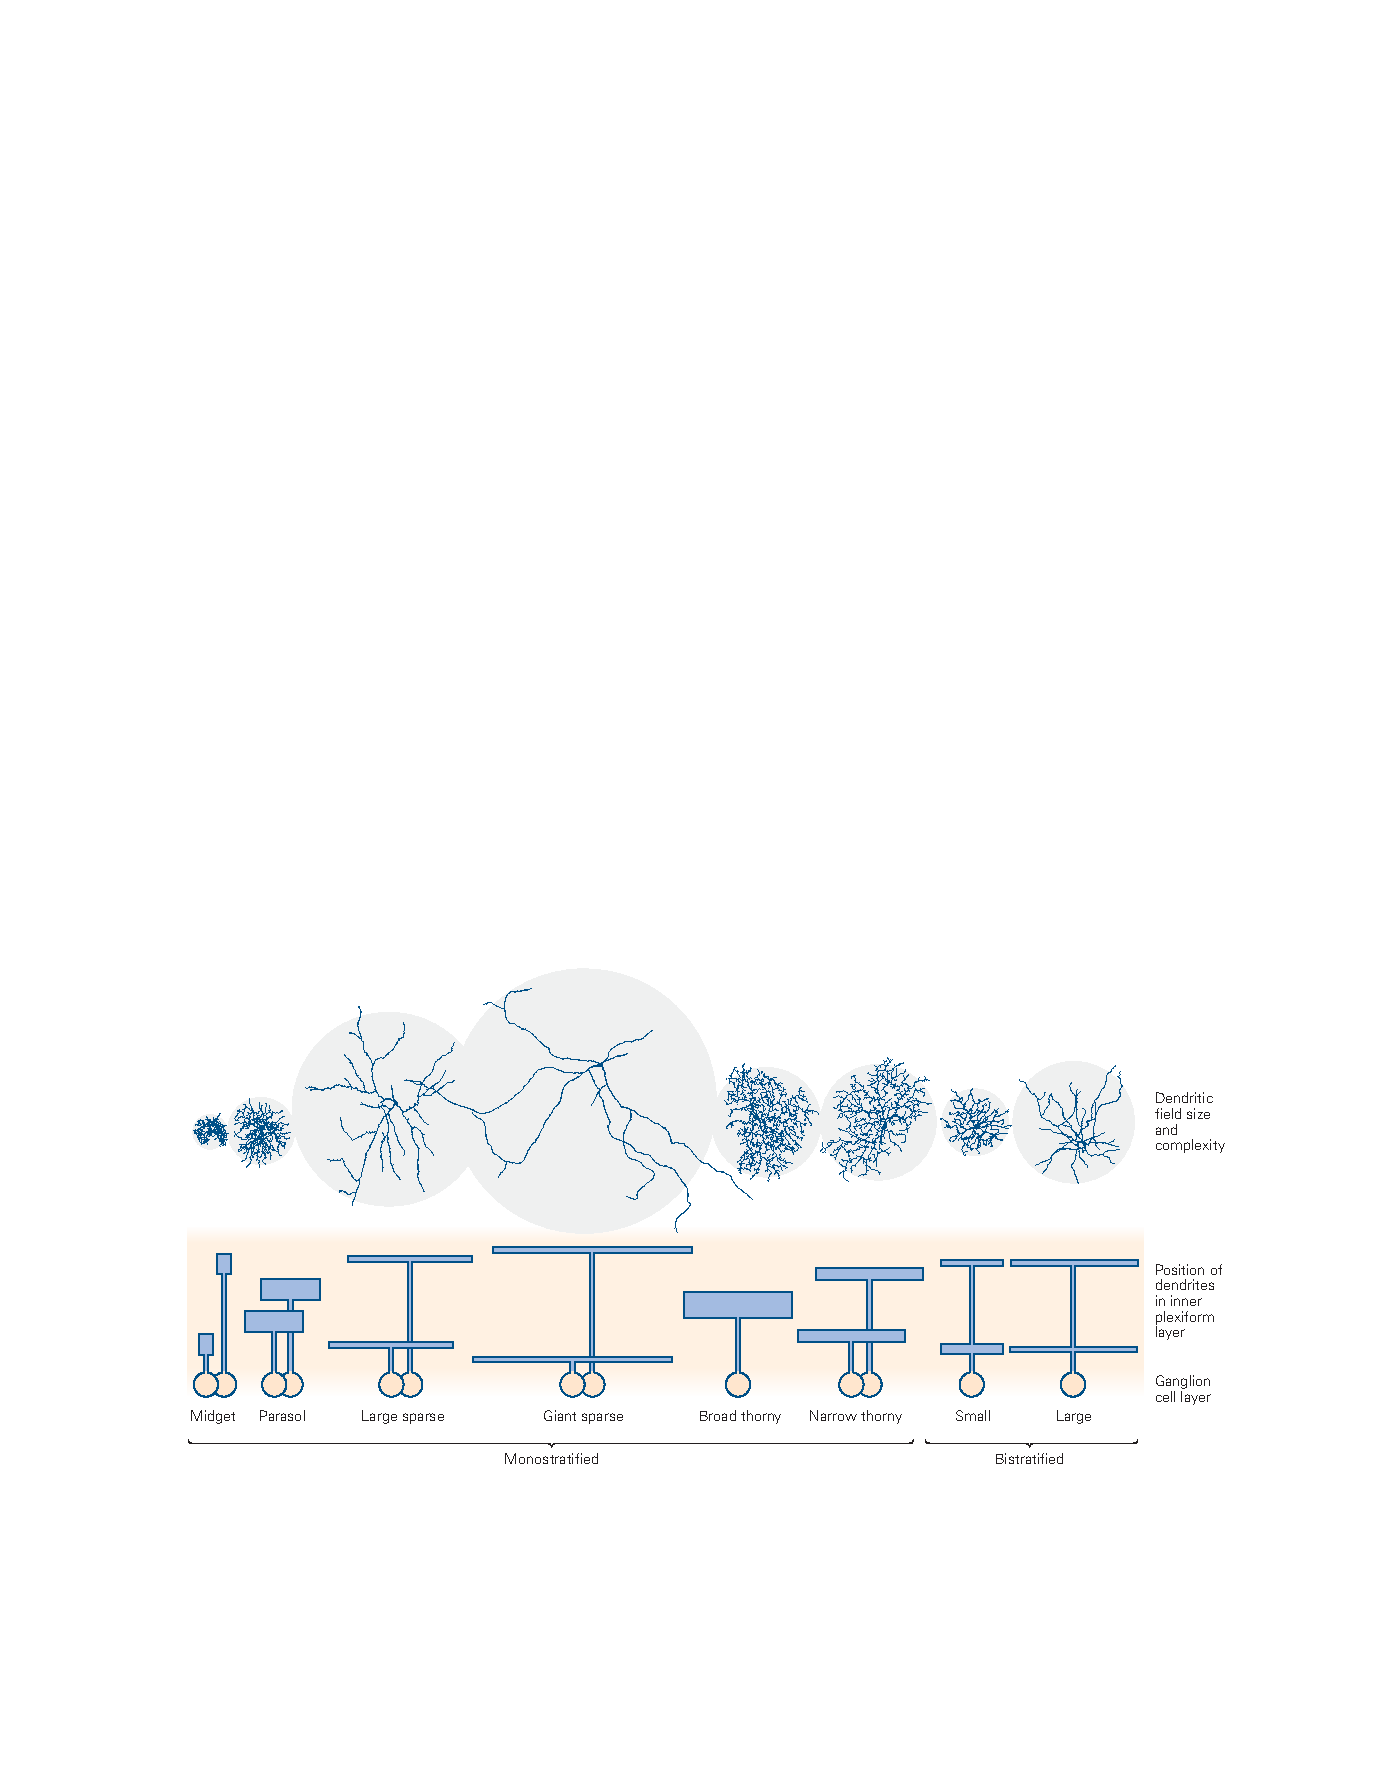
\includegraphics[width=1.0\linewidth]{chap03/fig_3_4}
	\caption{感觉神经元可以细分为功能不同的组。
		例如,至少有 13 种类型的视网膜神经节细胞是根据它们的树突的大小和形状以及它们接收输入信号的视网膜深度来区分的。
		内丛状层包含视网膜中间神经元(双极和无长突细胞)和神经节细胞之间的连接\cite{dacey2003fireworks}。}
	\label{fig:3_4}
\end{figure}


\subsection{神经胶质细胞支持神经细胞}
\textit{神经胶质细胞}的数量远远超过神经元,在脊椎动物中枢神经系统中,神经胶质细胞的数量是神经元的 2 到 10 倍。
尽管这些细胞的名称源自希腊语中的\textit{胶水},但胶质细胞通常不会将神经细胞聚集在一起。
相反,它们围绕着神经元的细胞体、轴突和树突。
胶质细胞在形态上不同于神经元,
它们不形成树突和轴突。


胶质细胞在功能上也有所不同。
尽管它们来自相同的胚胎前体细胞,但它们不具有与神经元相同的膜特性,因此不能是可兴奋的。
因此,它们不直接参与电信号传递,这是神经细胞的功能。
然而,它们在允许电信号沿着神经元的轴突快速移动方面发挥了作用,而且它们似乎在引导早期发育过程中的连接,以及稳固通过学习发生的神经元之间新的连接或改变的连接方面发挥了重要作用。
在过去的十年中,人们对胶质细胞的多种功能的兴趣有所增加,它们的特征已经从支持细胞转变为神经元的功能伙伴(第~\ref{chap:chap7}~章)。



\section{每个神经细胞都是调节特定行为的回路的一部分}

每种行为都由一组特定的相互连接的神经元介导,而每
一个神经元的行为功能都取决于它与其他神经元的联系。
一个简单的膝跳反射行为将说明这一点。 
当身体短暂的不平衡拉伸腿部股四头肌伸肌时,反射开始。
这种拉伸会产生传送给运动神经元的感觉信息,而运动神经元又会向伸肌发出收缩命令,从而恢复平衡。


这种反射在临床上用于测试神经的完整性以及反射幅度(或增益)的脑脊髓控制。 
潜在的机制很重要,因为它可以维持股四头肌的正常张力,并防止我们的膝盖在站立或行走时屈曲。 
股四头肌的肌腱,一种移动小腿的伸肌,通过髌骨(膝盖骨)的肌腱附着在胫骨上。 
轻敲髌骨正下方的肌腱可以拉伸股四头肌。 
这种拉伸启动股四头肌的反射性收缩,产生熟悉的膝跳。 
通过增加选定肌肉群的张力,牵张反射改变腿的位置,突然向外伸展(图 \ref{fig:3_5})。

\begin{figure}[htbp]
	\centering
	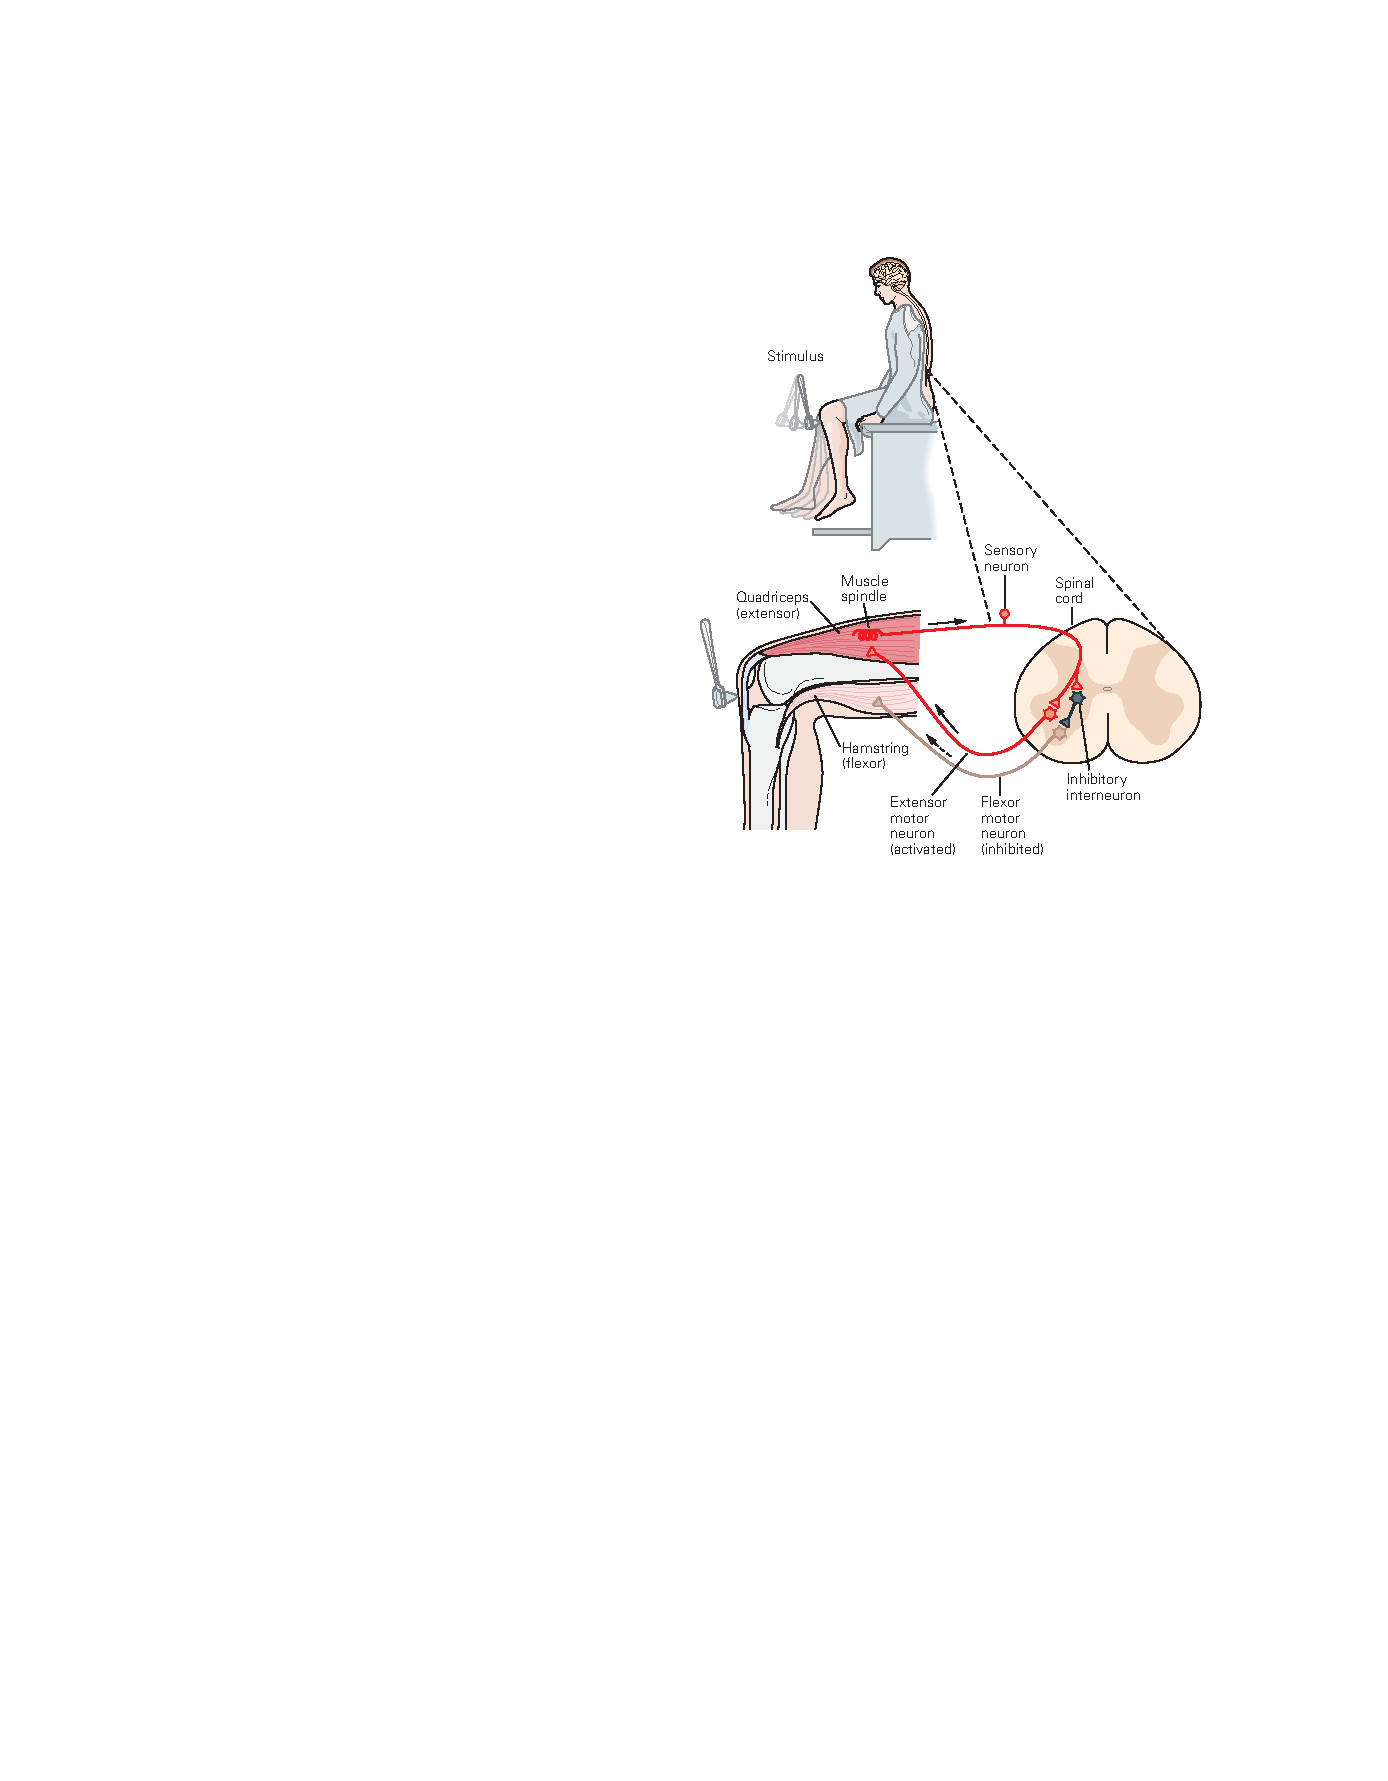
\includegraphics[width=0.6\linewidth]{chap03/fig_3_5}
	\caption{膝跳反射由感觉和运动神经元组成的简单回路控制。
		用反射锤轻敲膝盖骨,拉动股四头肌的肌腱,股四头肌是拉伸小腿的肌肉。
		当肌肉因肌腱的牵拉而伸展时,有关肌肉变化的信息会通过感觉神经元传送到中枢神经系统。
		在脊髓中,感觉神经元与收缩股四头肌(被拉伸的肌肉)的伸肌运动神经元形成兴奋性突触。 
		感觉神经元通过中间神经元间接作用,抑制屈肌运动神经元,否则这些神经元会收缩相对的腿筋肌肉。 
		这些动作结合起来产生反射行为。 
		在图中,每个伸肌和屈肌运动神经元代表许多细胞群。}
	\label{fig:3_5}
\end{figure}


参与膝跳反射的感觉神经元细胞体聚集在背根神经节的脊髓附近。
它们是假单极细胞;
每个细胞轴突的一个分支延伸到周围的股四头肌,而另一个延伸到脊髓的中央。
支配股四头肌的分支与拉伸敏感受体(肌梭)接触,并在肌肉拉伸时兴奋。 
到达脊髓的分支与支配股四头肌并控制其收缩的运动神经元形成兴奋性连接。 
该分支还联系抑制控制相对屈肌的运动神经元的局部中间神经元(图~\ref{fig:3_5})。 
尽管这些局部中间神经元本身不参与牵张反射的产生,但它们通过协调相反肌肉群的动作来增加反射的稳定性。 
因此,产生牵张反射的电信号携带四种信息:

1. 感觉信息从肌肉传递到中枢神经系统(脊髓)。

2. 来自中枢神经系统的运动命令被发送到进行膝跳的肌肉。

3. 向支配相反肌肉的运动神经元发出抑制性命令。

4. 与膝跳有关的局部神经元活动的信息被发送到中枢神经系统的更高中枢,允许大脑同时或依次协调不同的行为。


此外,大脑声称依赖于上下文的反射控制来调整其增益。
例如,当我们跑步时,腘绳肌会弯曲膝盖,从而拉伸股四头肌。
大脑和脊髓抑制牵张反射,使股四头肌放松。 
当这些下行通路被破坏时,就像在某些划水动作中一样,反射被放大并且关节变得僵硬。


仅仅拉伸一块肌肉,股四头肌,就会激活数百个感觉神经元,每个神经元与 45 到 50 个运动神经元直接接触。 
这种连接模式,其中一个神经元激活许多目标细胞,称为发散(图 \ref{fig:3_6}A)。 
它在神经系统的输入阶段尤为常见; 通过将其信号分配给许多靶细胞,单个神经元可以发挥广泛而多样的影响。 
相反,膝跳回路中的单个运动细胞从大约 130 个感觉细胞接收 200 到 450 个输入触点。 
这种连接模式称为收敛(图 \ref{fig:3_6}B)。 
它在神经系统的输出阶段很常见; 从许多感觉神经元接收信息的目标运动细胞能够整合来自许多来源的信息。 
每个感觉神经元输入产生相对较弱的兴奋,因此收敛也确保只有当足够数量的感觉神经元一起被激活时,运动神经元才会被激活。


\begin{figure}[htbp]
	\centering
	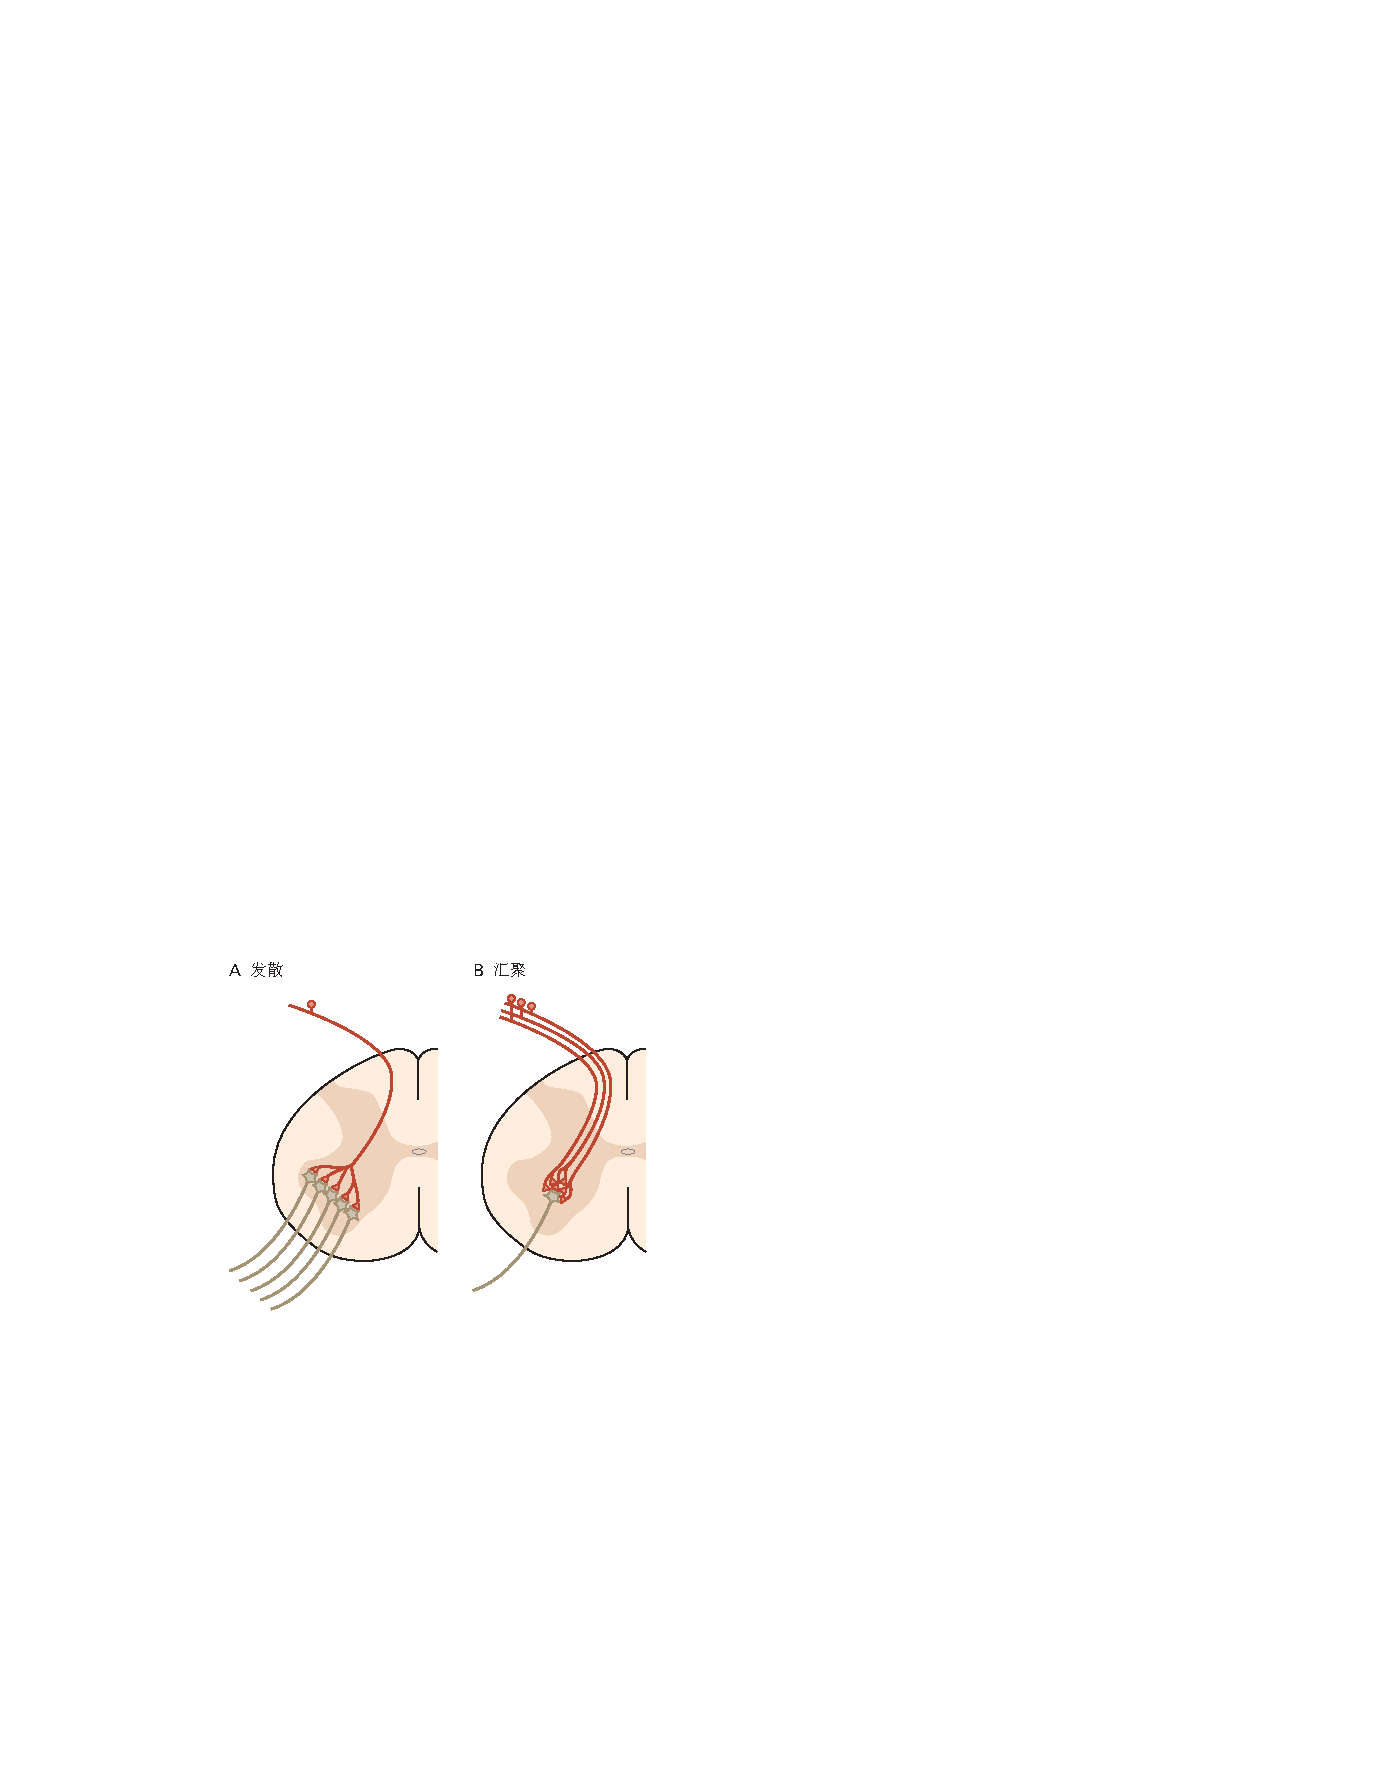
\includegraphics[width=0.5\linewidth]{chap03/fig_3_6}
	\caption{发散和会聚的神经元连接是大脑的一个关键组织特征。
		\textbf{A.} 在感觉系统中,每个受体神经元通常与代表第二阶段处理的几个神经元联系。 
		在随后的处理阶段,传入的连接更加分散。 
		这使得来自单个站点的感觉信息可以更广泛地分布在脊髓和大脑中。 
		\textbf{B.} 相比之下,运动神经元是逐渐融合连接的目标。 
		通过这种安排,需要来自许多突触前细胞的输入来激活运动神经元。}
	\label{fig:3_6}
\end{figure}


诸如膝跳反射之类的牵张反射是由在兴奋性突触处连接的两类神经元产生的一种简单行为。 
但并非大脑中的所有重要信号都是兴奋性的。 
许多神经元会产生抑制信号,从而降低放电的可能性。 
即使在简单的膝跳反射中,感觉神经元也会产生兴奋性和抑制性连接。 
腿部伸肌中的兴奋性连接会导致这些肌肉收缩,而与抑制性中间神经元的连接会阻止拮抗性屈肌收缩。 
回路的这个特性是前馈抑制的一个例子(图~\ref{fig:3_7}A)。 
在膝跳反射中,前馈抑制是相互的,确保屈肌和伸肌通路始终相互抑制,以便只招募适合运动的肌肉,而不是那些反对运动的肌肉。


\begin{figure}[htbp]
	\centering
	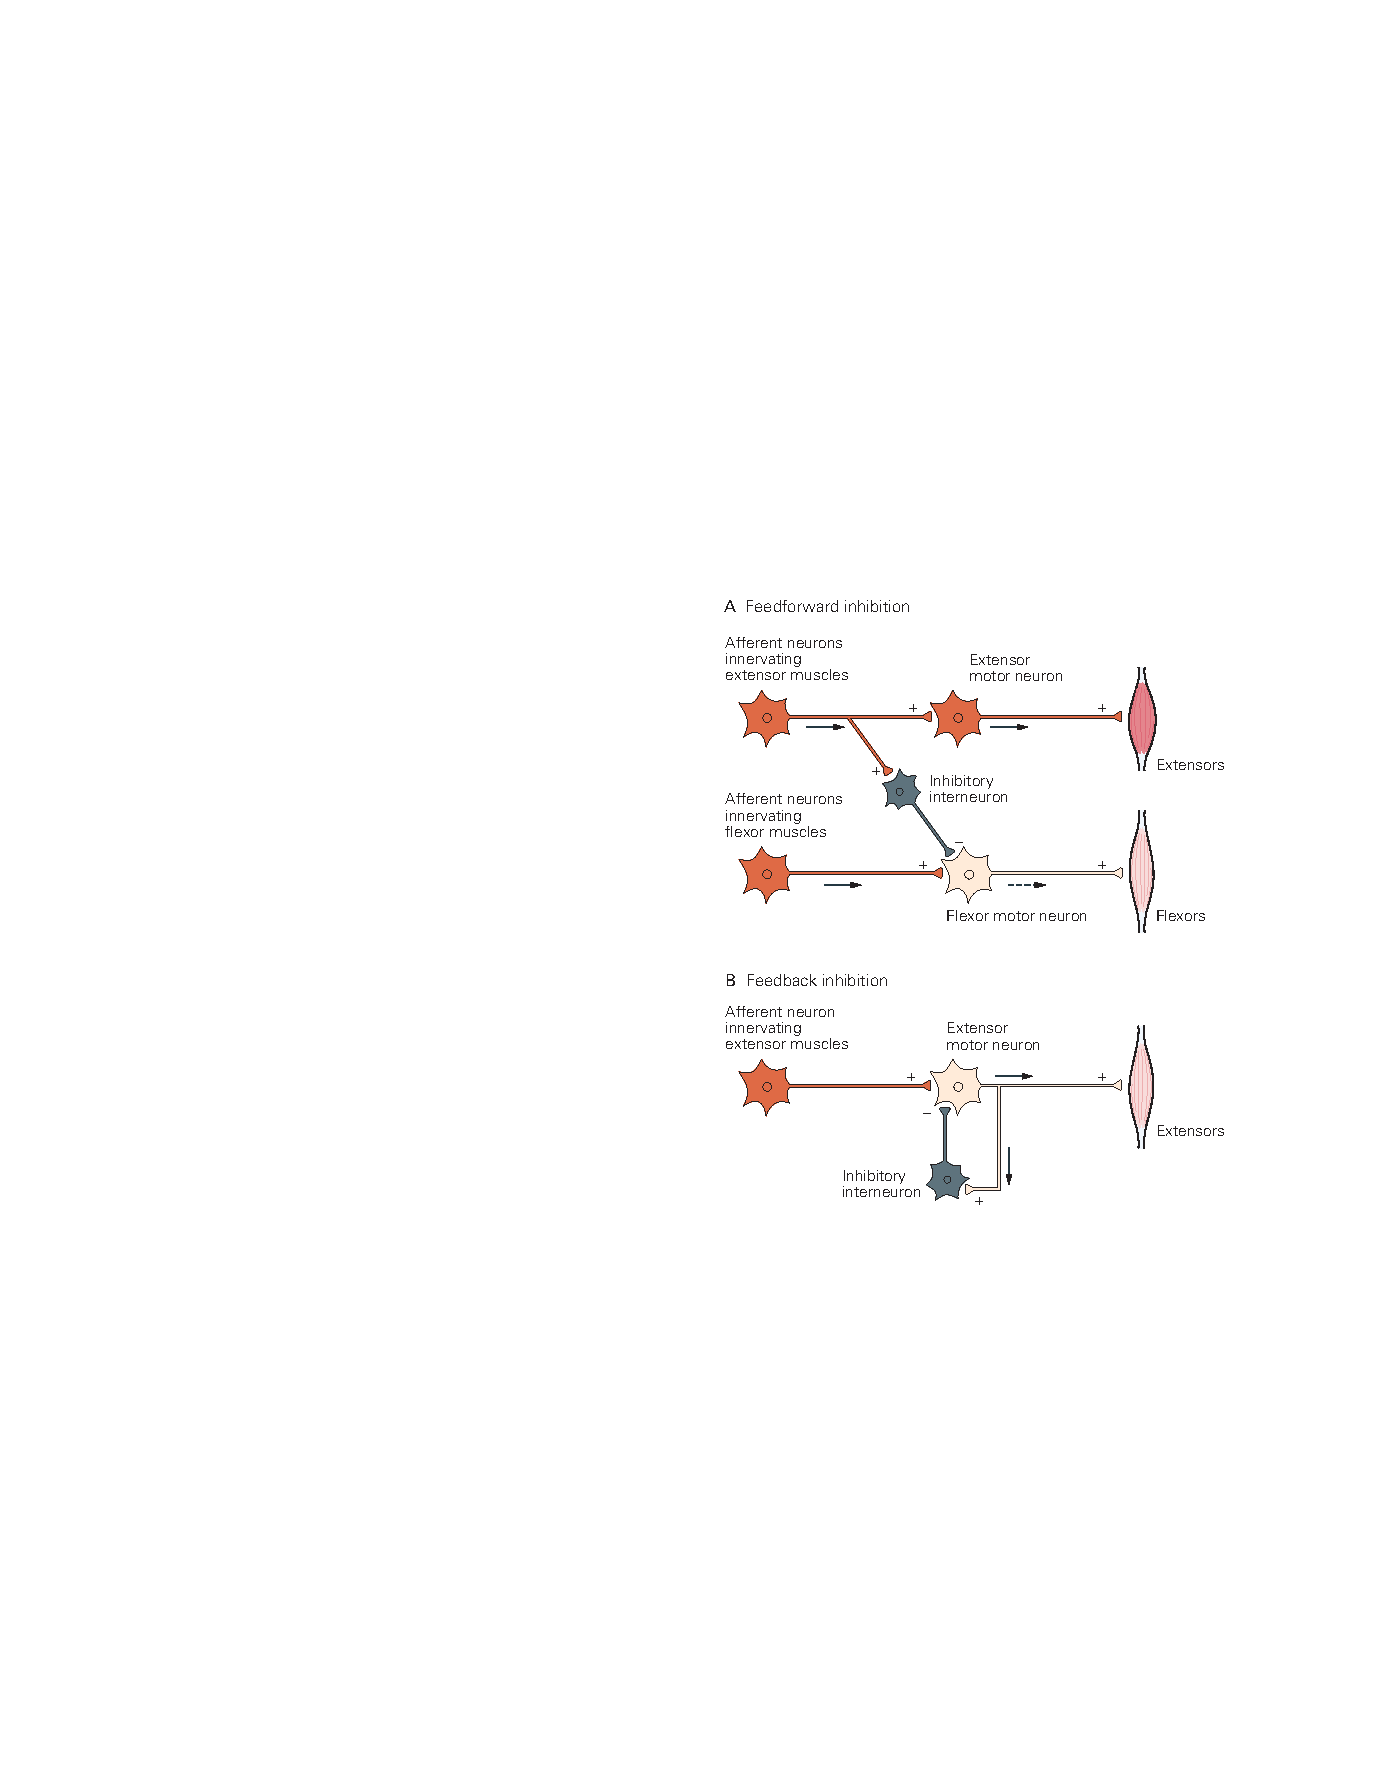
\includegraphics[width=0.55\linewidth]{chap03/fig_3_7}
	\caption{抑制性中间神经元可以产生前馈或反馈抑制。
		\textbf{A.} 前馈抑制通过抑制调节相反作用的通路的活性来增强活性通路的效果。
		前馈抑制在单突触反射系统中很常见。 
		例如,在膝跳反射回路(图~\ref{fig:3_5})中,来自伸肌的传入神经元不仅会刺激伸肌运动神经元,还会刺激抑制性中间神经元,从而阻止神经支配相对屈肌的运动细胞的放电。 
		\textbf{B.} 反馈抑制是一种自我调节机制。
		在这里,伸肌运动神经元作用于抑制性中间神经元,后者反过来作用于伸肌运动神经元本身,从而降低它们放电的可能性。
		其作用是抑制受刺激通路内的活动并防止其超过某个临界水平。}
	\label{fig:3_7}
\end{figure}


一些回路提供反馈抑制。 
例如,运动神经元可能与肌肉和抑制性中间神经元都有兴奋性连接,后者本身与运动神经元形成连接。 
当抑制性中间神经元被运动神经元兴奋时,中间神经元能够限制运动神经元兴奋肌肉的能力(图 \ref{fig:3_7}B)。 
当我们在后面的章节中研究更复杂的行为时,我们会遇到许多前馈和反馈抑制的例子。


\section{信号在所有神经细胞中的组织方式相同}
为了产生一种行为,例如牵张反射,每个参与的感觉和运动神经细胞必须依次产生四种不同的信号,每个信号位于细胞内的不同位置。 
尽管细胞大小和形状、递质生物化学或行为功能各不相同,但几乎所有神经元都可以用一个模型神经元来描述,该模型神经元具有产生四种类型信号的四个功能组件:
一个用于产生分级输入信号的接收组件,一个求和或 产生触发信号的综合组件,产生全或无传导信号的传导远程信号组件,以及产生输出信号到下一个神经元或肌肉或腺体细胞的突触组件(图~\ref{fig:3_8})。


\begin{figure}[htbp]
	\centering
	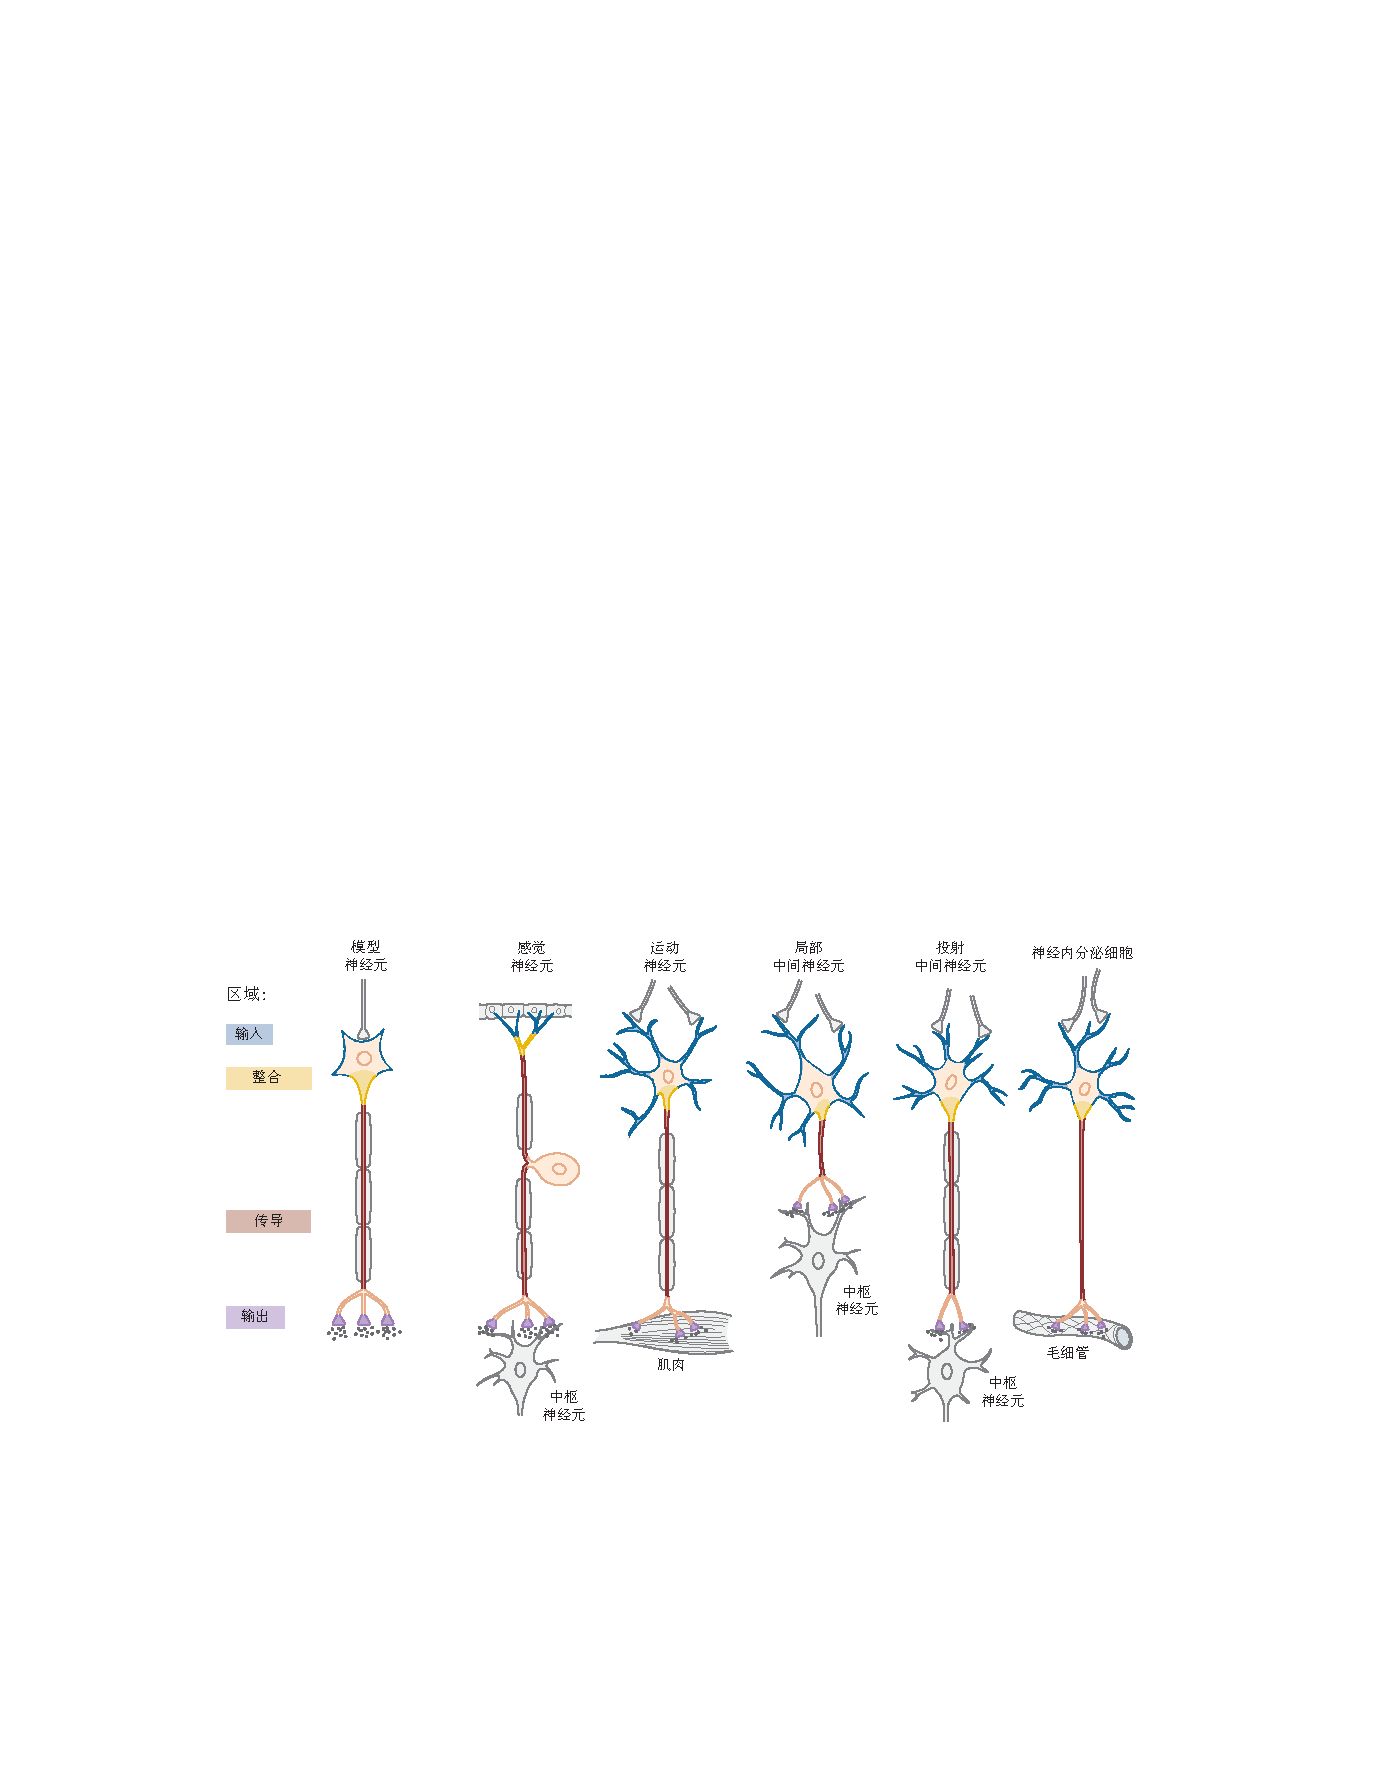
\includegraphics[width=0.8\linewidth]{chap03/fig_3_8}
	\caption{大多数神经元有四个功能区域,在这些区域中会生成不同类型的信号。 
		因此,大多数神经元的功能组织,无论类型如何,都可以用模型神经元示意性地表示。 
		该模型神经元是\textit{拉蒙-卡哈尔}动态极化原理的生理表达。 
		输入信号、综合信号和传导信号都是电信号,对细胞来说是不可或缺的,而输出信号是由细胞射入突触间隙的化学物质。 
		并非所有神经元都具有所有这些特征。 
		例如,一些局部中间神经元缺乏导电成分。}
	\label{fig:3_8}
\end{figure}


神经元中产生的不同类型的信号部分取决于细胞膜的电特性。 
当细胞处于静止状态时,包括神经元在内的每个细胞都在质膜两侧保持一定的电位差。 
这称为静息膜电位。 
在典型的静息神经元中,细胞内部的电压比细胞外部的电压负大约 65 毫伏。
因为膜外电压被定义为零,所以我们说静息膜电位为 –65 毫伏。 
不同神经细胞的静息电位范围为 –40 毫伏至 –80 毫伏; 
在肌肉细胞中,它更大,约为 –90 毫伏。 
正如第~\ref{chap:chap9}~章中详细描述的,静息膜电位由两个因素造成:
带电离子的不均匀分布,特别是带正电的 \ce{Na+} 和 \ce{K+},以及膜的选择性渗透性。


带正电的离子在细胞膜两侧的不均匀分布由两个主要机制维持。 
细胞内 \ce{Na+} 和 \ce{K+} 浓度主要由膜蛋白控制,膜蛋白主动将 \ce{Na+} 泵出细胞并将 \ce{K+} 泵回细胞内。 
这个 \ce{Na+}-\ce{K+} 泵,我们将在第 \ref{chap:chap9} 章中详细了解,它使细胞内的 \ce{Na+} 浓度保持在较低水平(约为细胞外浓度的十分之一),并使 \ce{K+} 浓度保持在较高水平(约为细胞外浓度的 20 倍)。 
\ce{Na+} 和 \ce{K+} 的细胞外浓度由肾脏和星形胶质细胞(也称为星形胶质细胞)维持。


否则不可渗透的细胞膜含有形成称为离子通道的孔的蛋白质。 细胞静止时活跃的通道对 \ce{K+} 的渗透性很高,但对 \ce{Na+} 的渗透性要低得多。 
\ce{K+} 离子往往会沿着离子的浓度梯度从这些开放通道中泄漏出来。 
当 \ce{K+} 离子离开细胞时,它们会在膜的内表面留下一团未中和的负电荷,因此膜内的净电荷比膜外的负电荷更多。 
在这种情况下,相对于神经元外部,膜电位通常保持在 –65 毫伏左右,据说神经元处于静止状态。


当细胞开始吸收细胞外浓度较高的 \ce{Na+}(或钙离子)时,静息状态就会受到干扰。 
这些带正电的离子向内运动(内向电流)部分地中和了细胞内部的负电压。 
我们将在下面详细介绍这些事件。 
然而,接下来发生的事情是理解神经元是什么使信号适合传递信息的关键。


当一个细胞,如神经和肌肉,其膜电位可以迅速而显着地改变时,就被认为是可兴奋的。 
在许多神经元中,膜电位 10 毫伏的变化(从 –65 毫伏到 –55 毫伏)使膜对 \ce{Na+} 的渗透性比对 \ce{K+} 的渗透性强得多。 
由此产生的 \ce{Na+} 流入进一步中和了细胞内的负电荷,导致对 \ce{Na+} 的渗透性更高。 
结果是膜电位发生短暂的爆炸性变化,变为 +40 毫伏,即动作电位。 
这种电位被积极地沿着细胞的轴突传导到轴突的末端,在那里它启动与突触后神经元或肌肉细胞的精细化学相互作用。 
由于动作电位是主动传播的,因此其振幅在到达轴突末端时不会减小。 
动作电位通常持续约 1 毫秒,之后膜恢复到其静止状态,电荷正常分离,对 \ce{K+} 的渗透性高于对 \ce{Na+} 的渗透性。


静息电位和动作电位的潜在机制在第 \ref{chap:chap9} 章和第 \ref{chap:chap10} 章中详细讨论。
除了动作电位代表的长距离信号外,神经细胞还产生局部信号——受体电位和突触电位——这些信号不活跃 传播并且通常在几毫米内衰减(见下一节)。


产生远程和局部信号的膜电位变化可以是静息电位的降低或增加。 
也就是说,静息膜电位是所有信号发生的基线。 
膜电位的降低(称为去极化)增强了细胞产生动作电位的能力,因此具有兴奋性。 
相反,膜电位的增加,称为超极化,使细胞不太可能产生动作电位,因此具有抑制作用。


\subsection{输入组件产生分级本地信号}
在大多数静止的神经元中,没有电流从细胞的一部分流向另一部分,因此静息电位始终相同。 
在感觉神经元中,电流通常由物理刺激启动,物理刺激会激活神经元接受表面的特殊受体蛋白。 
在我们膝跳反射的例子中,肌肉的拉伸会激活特定的离子通道,这些离子通道会响应感觉神经元膜的拉伸而打开,我们将在第~\ref{chap:chap18}~章中了解到。
当细胞被拉伸时,这些通道的打开允许 \ce{Na+} 离子快速流入感觉细胞。 
这种离子电流改变膜电位,产生称为受体电位的局部信号。


受体电位的幅度和持续时间取决于肌肉拉伸的强度:拉伸越大或持续时间越长,由此产生的受体电位越大或持续时间越长(图~\ref{fig:3_9}A)。
也就是说,受体电位是分级的,这与\textit{全有或全无}动作电位不同。
大多数受体电位是去极化的(兴奋性的);
在视网膜中发现超极化(抑制)受体电位。


\begin{figure}[htbp]
	\centering
	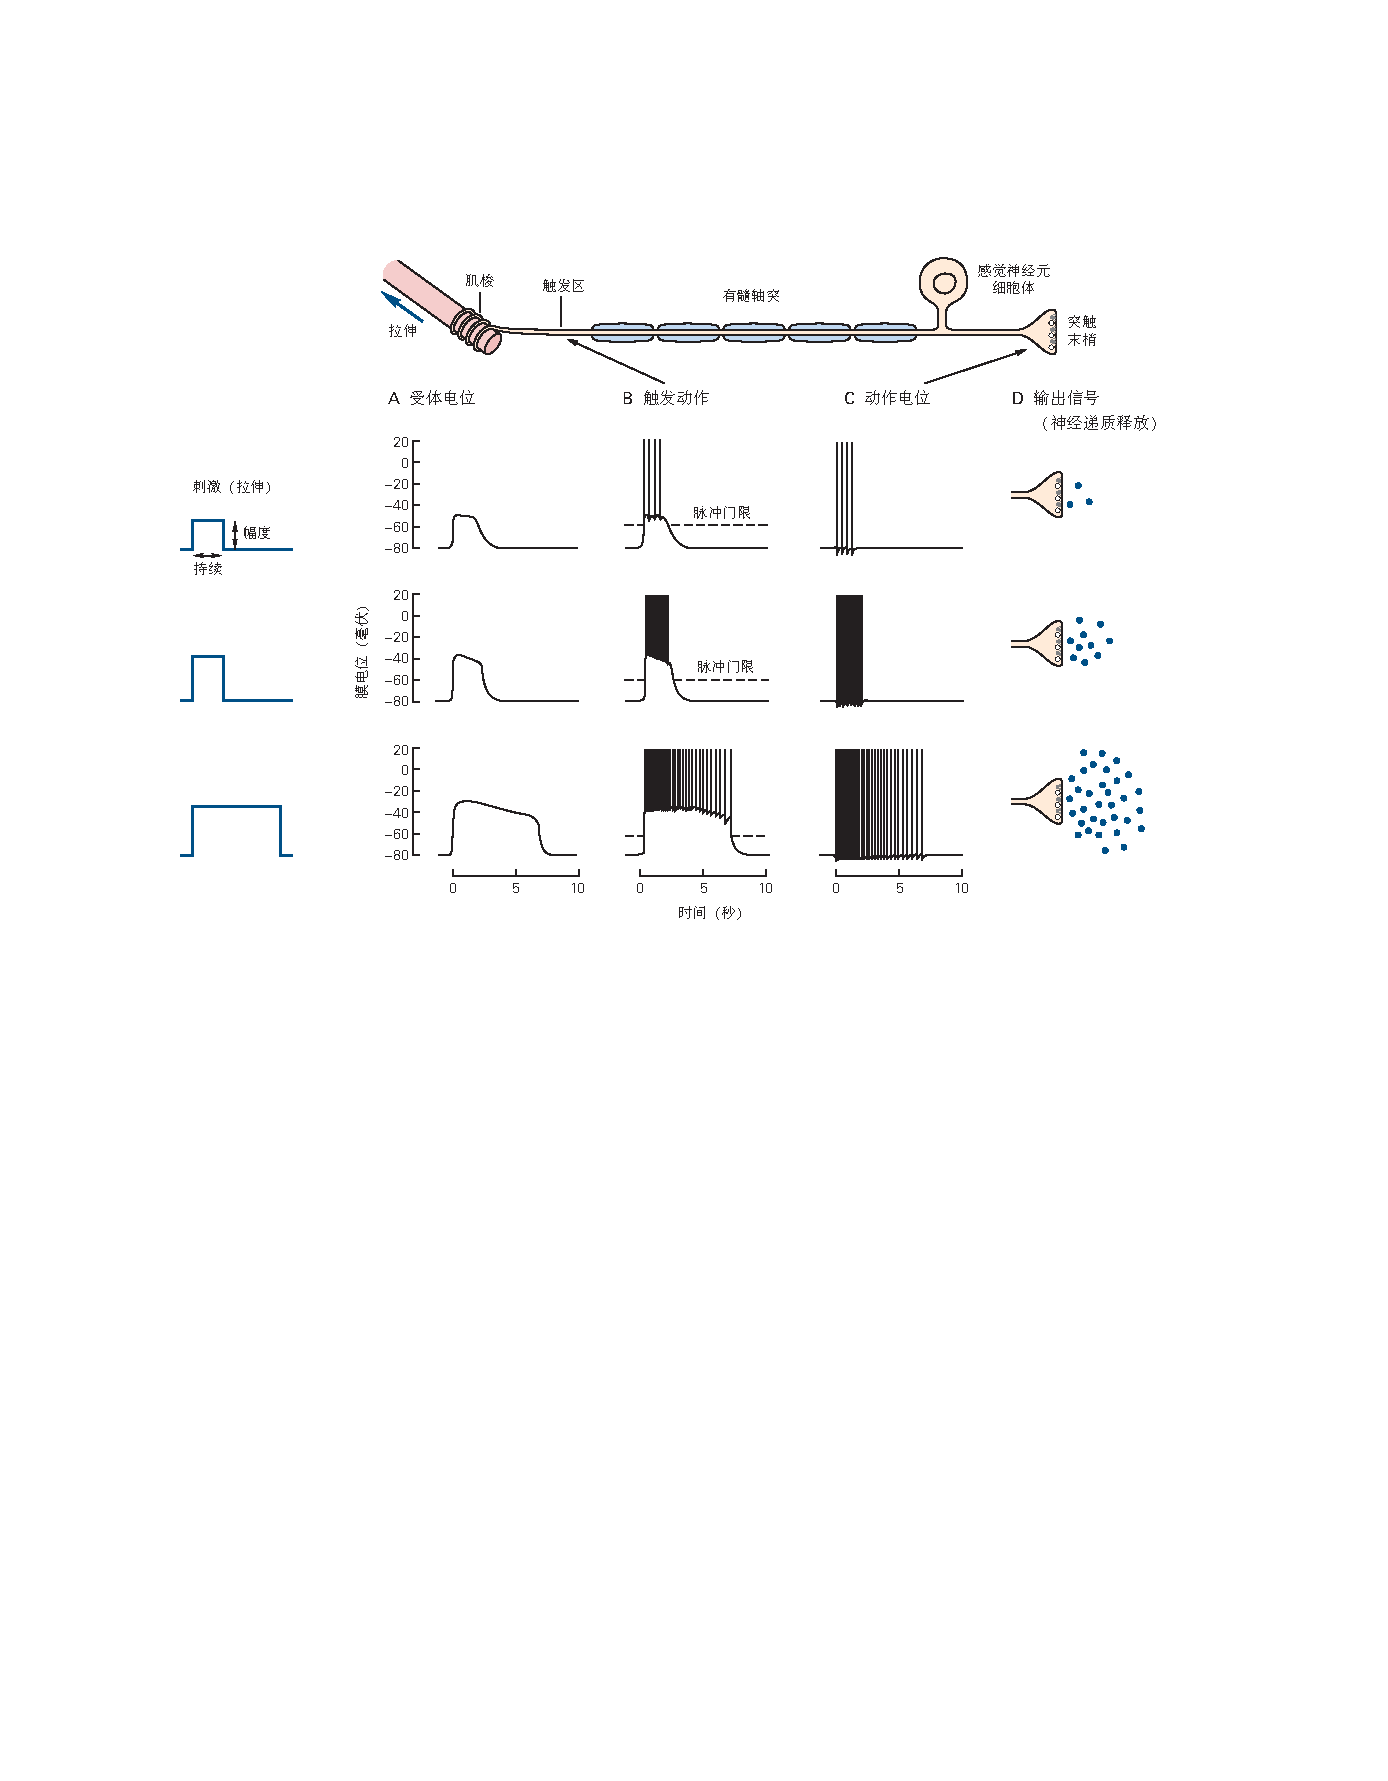
\includegraphics[width=1.0\linewidth]{chap03/fig_3_9}
	\caption{神经元的四个信号成分中的每一个都会产生一个特征信号。
		该图显示了通过肌肉拉伸激活的感觉神经元,神经元通过专门的受体(肌梭)感知。 
		\textbf{A.} 输入信号,称为受体电位,在振幅和持续时间上分级,与刺激的振幅和持续时间成正比。 
		\textbf{B.} \textit{触发区}总结了受体电位产生的去极化。
		只有当受体电位超过某个电压阈值时才会产生动作电位。
		一旦超过这个阈值,受体电位幅度的任何进一步增加只能增加动作电位产生的频率,因为动作电位具有恒定的幅度。
		受体电位的持续时间决定了动作电位序列的持续时间。
		因此,受体电位的分级振幅和持续时间被转化为触发区产生的动作电位中的频率代码。
		产生的所有动作电位都忠实地沿着轴突传播。
		\textbf{C.} 动作电位是全有或全无。
		因为所有动作电位都具有相似的幅度和持续时间,所以放电的频率和持续时间编码了信号所携带的信息。
		\textbf{D.} 当动作电位到达突触末梢时,它会启动神经递质的释放,即用作输出信号的化学物质。
		突触前细胞中动作电位的频率决定了细胞释放多少神经递质。}
	\label{fig:3_9}
\end{figure}


受体电位是在神经系统中编码的第一个拉伸表示。
然而,由于这种去极化从拉伸感受器被动传播,它不会传播很远。
如果轴突的直径较大,则距离较长,如果直径较小,则距离较短。
此外,如果电流可以轻松通过膜,则距离会更短,如果膜被髓磷脂绝缘,则距离会更长。
因此,来自拉伸感受器的感受器电位仅移动 1 至 2 毫米。
事实上,就在 1 毫米远的地方,信号的幅度仅为产生位置的三分之一左右。 
为了成功地传送到脊髓,局部信号必须被放大——它必须产生动作电位。
在膝跳反射中,如果感觉神经元中的受体电位到达轴突中朗飞的第一个节点并且足够大,它将触发动作电位(图~\ref{fig:3_9}B),然后无故障地传播到轴突 脊髓中的末端(图~\ref{fig:3_9}C)。 
在感觉神经元和运动神经元之间的突触处,动作电位会产生一系列事件,这些事件会导致运动神经元的输入信号。


在膝跳反射中,感觉神经元突触前末梢的动作电位启动化学物质或神经递质释放到突触间隙(图~\ref{fig:3_9}D)。
扩散穿过裂隙后,递质与运动神经元突触后膜中的受体蛋白结合,从而直接或间接打开离子通道。
随后的电流流动会短暂地改变运动细胞的膜电位,这种变化称为突触电位。


与受体电位一样,突触电位也是分级的; 
它的振幅取决于释放发射器的量。 
在同一细胞中,突触电位可以去极化或超极化,具体取决于被激活的受体分子的类型。 
突触电位,如受体电位,被动传播。 
因此,电位的变化将保持局部,除非信号超出轴突的初始段,在那里它可以产生动作电位。 
一些树突并非完全被动,而是包含促进突触电位的特化,从而提高其产生动作电位的功效(第~\ref{chap:chap13}~章)。 
表~\ref{tab:3_1}~总结了受体和突触电位的特征。


\begin{table}[htbp]
	\caption{局部(被动)和传播信号的比较} \label{tab:3_1} \centering
	\begin{tabular}{llllll}
		\toprule
		信号类型 & 幅值(毫伏) & 持续时间 & 总和 & 信号效应 & 传播类型\\
		\midrule
		\makecell{局部被动信号\\受体电位} & 小(0.1–10) & 短暂(5-100毫秒) & 分级 & 超级化或去极化 & 被动 \\
		\midrule
		突触电位 & 由短到长 & 短暂(5-100毫秒) & 分级 & 超级化或去极化 & 被动 \\
		\makecell{传播(激活)的信号\\动作电位} & 大(70–110) & 短暂(1-10毫秒) & 全有或全无 & 
		去极化 & 主动 \\
		\bottomrule
	\end{tabular}
\end{table}


\subsection{触发区决定产生动作电位}
谢林顿首先指出,神经系统的功能是权衡不同类型信息的后果,然后决定适当的反应。 
神经系统的这种整合功能在神经元触发区(轴突的初始部分)的事件中清晰可见。


动作电位是由 \ce{Na+} 通过细胞膜中的通道突然流入而产生的,这些通道响应于膜电位的变化而打开和关闭。 
当输入信号(受体电位或突触电位)使膜区域去极化时,膜电位的局部变化会打开局部 \ce{Na+} 通道,使 \ce{Na+} 沿着其浓度梯度从 \ce{Na+} 浓度高的细胞外流到细胞内 它低的地方。


由于轴突的起始段具有最高密度的电压敏感 \ce{Na+} 通道,因此产生动作电位的阈值最低,因此沿细胞膜被动传播的输入信号更有可能在起始段产生动作电位轴突的部分比在细胞中的其他部位。
因此,这部分轴突被称为触发区。
所有受体(或突触)电位的活动都在这里求和,如果输入信号的总和达到阈值,神经元就会产生动作电位。


\subsection{导电成分传播全有或全无动作电位}
动作电位是全有或全无:
低于阈值的刺激不会产生信号,但高于阈值的刺激都会产生相同幅度的信号。
无论刺激强度或持续时间的变化如何,每个动作电位的幅度和持续时间几乎相同,这适用于沿着有髓轴突的朗飞节点处的每个再生动作电位。
此外,与被动传播和振幅减小的受体和突触电位不同,正如我们所见,动作电位在沿着轴突到达其目标(距离可达 1 米)时不会衰减。 
因为它是周期性再生的。
这种传导信号可以以高达 100 米每秒的速度传播。 
事实上,动作电位的显着特征是它们是高度刻板的,从一个神经细胞到另一个神经细胞的变化很小(但在某些情况下很重要)。 
\textit{埃德加·阿德里安}在 1920 年代证明了这一特征,他是最早在细胞水平上研究神经系统的人之一。
阿德里安发现所有动作电位都具有相似的形状或波形(见图~\ref{fig:3_2})。
由感觉轴突带入神经系统的动作电位与由运动轴突从神经系统带入肌肉的动作电位通常无法区分。


传导信号只有两个特征传达信息:动作电位的数量和它们之间的时间间隔(图~\ref{fig:3_9}C)。 
正如\textit{阿德里安}在 1928 年总结他对感觉纤维的研究时所说:“所有的冲动都非常相似,无论信息是注定要引起光感、触感还是痛感;
如果它们挤在一起,感觉就会强烈,如果它们相距很远,感觉就会相应地微弱。” 
因此,决定感觉强度或运动速度的是动作电位的频率。
同样,感觉或运动的持续时间由产生动作电位的时间段决定。


除了动作电位的频率,动作电位的模式也传达了重要的信息。
例如,一些神经元在没有刺激的情况下会自发活跃。
一些自发活跃的神经细胞(跳动的神经元)有规律地激发动作电位;
其他人(爆发的神经元)在短暂的动作电位爆发中发射。
这些不同的细胞对相同的兴奋性突触输入有不同的反应。
兴奋性突触电位可能会在一个非自发活跃的细胞中启动一个或多个动作电位,而对自发活跃细胞的相同输入只会增加现有的放电率。


当输入信号具有抑制性时,会出现更显着的差异。
抑制性输入在沉默细胞中几乎没有信息价值。 
相比之下,在自发活跃的细胞中,抑制可以起到强大的塑造作用。
通过在其他正在进行的活动中建立沉默期,抑制可以在不存在的地方产生一种复杂的交替放电和沉默模式。
放电模式的这种细微差异可能对神经元之间的信息传递产生重要的功能影响。
神经元网络的数学建模者试图描述神经代码,其中信息也由细粒度的放电模式——每个动作电位的确切时间——携带。


如果信号是固定的并且仅反映刺激的最基本属性,那么它们如何携带复杂行为所需的丰富信息呢?
如何将包含蜜蜂视觉信息的信息与包含蜜蜂蜇伤疼痛信息的信息区分开来?
这些感觉信号与自主运动的运动信号有何区别? 
答案很简单,但却是神经系统最重要的组织原则之一:
相互连接的神经元形成解剖学和功能上不同的通路——标记线——正是这些连接神经元的通路,这些标记线,而不是单个神经元都传达信息。 
视网膜中对光有反应的受体细胞激活的神经通路与皮肤中对触觉有反应的感觉细胞激活的神经通路完全不同。


\subsection{输出组件释放神经递质}

当动作电位到达神经元的末端时,它会刺激细胞释放化学物质。
这些物质称为神经递质,可以是有机小分子,例如L-谷氨酸和乙酰胆碱,也可以是肽,例如 P 物质或 \textit{黄体生成素-释放激素}。


神经递质分子存在于称为突触小泡的亚细胞器中,突触小泡聚集在轴突末端的特殊释放部位,称为活性区。
为了将它们的递质物质喷射到突触间隙中,囊泡向上移动并与神经元的质膜融合,然后通过已知的过程突然打开以将递质释放到突触间隙(突触前细胞和突触后细胞之间的细胞外空间)中作为胞吐作用。
第~\ref{chap:chap14}~章和第~\ref{chap:chap15}~章描述了神经递质释放的分子机制。


释放的神经递质分子是神经元的输出信号。 
因此,输出信号根据释放的递质量进行分级,递质量由到达突触前末梢的动作电位的数量和频率决定(图~\ref{fig:3_9}C,D)。
释放后,递质分子扩散穿过突触间隙并与突触后神经元上的受体结合。
这种结合导致突触后细胞产生突触电位。
突触电位是否具有兴奋或抑制作用取决于突触后细胞中受体的类型,而不取决于特定的化学神经递质。
相同的递质物质在不同的受体上可能有不同的作用。



\subsection{牵张反射通路说明了神经信号从感觉到运动的转变}

正如我们所见,当信号从神经元的一个组成部分移动到另一个组成部分或在神经元之间移动时,信号的属性会发生变化。 
在牵张反射中,当肌肉被拉伸时,刺激的幅度和持续时间反映在感觉神经元中产生的受体电位的幅度和持续时间中(图~\ref{fig:3_10}A)。
如果受体电位超过该细胞中动作电位的阈值,则分级信号会在触发区转换为动作电位。
尽管个体动作电位是全有或全无信号,但受体电位超过阈值越多,去极化越大,因此轴突中动作电位的频率就越高。
输入信号的持续时间也决定了动作电位序列的持续时间。


\begin{figure}[htbp]
	\centering
	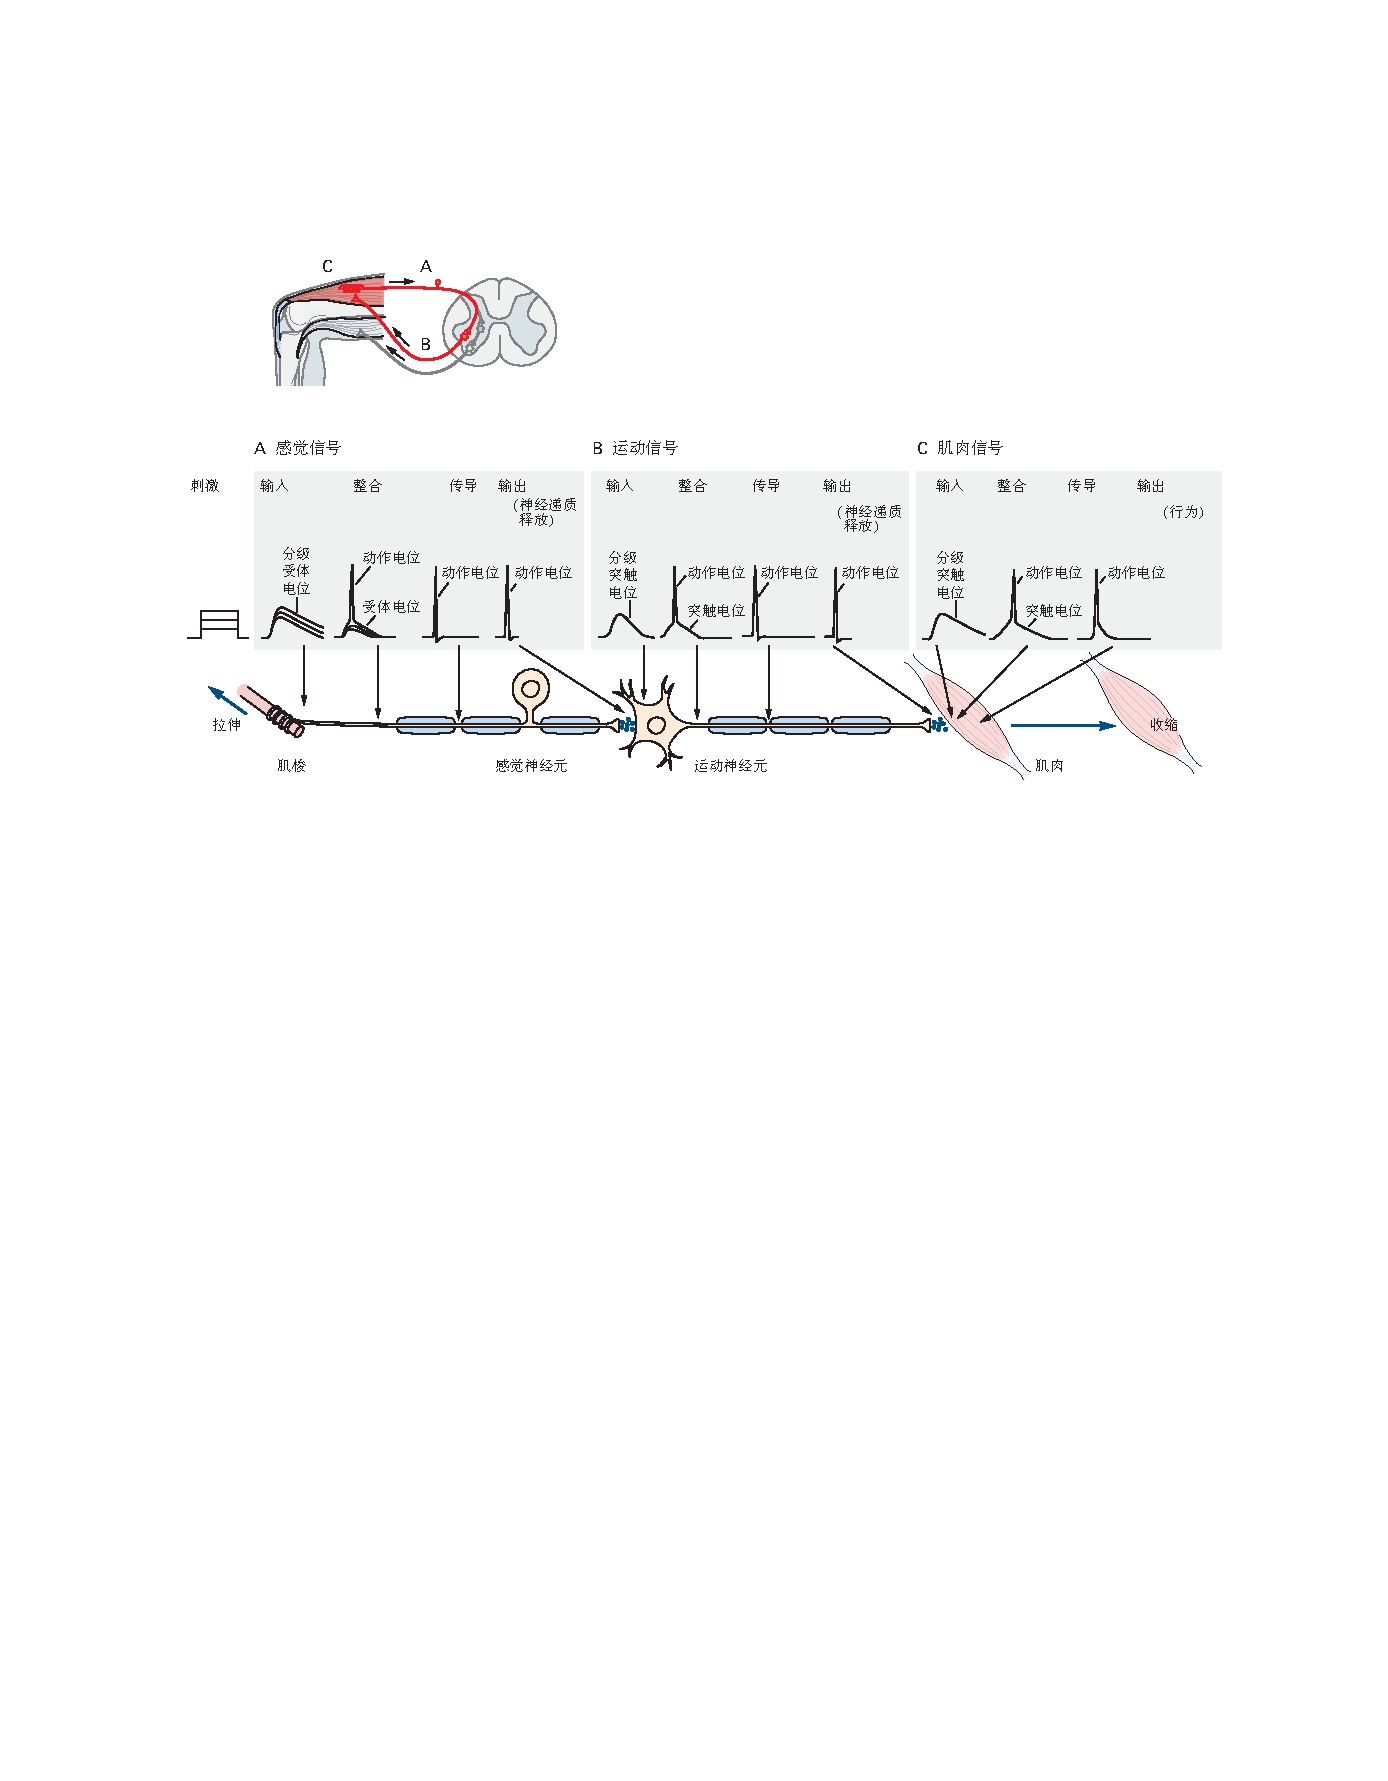
\includegraphics[width=1.0\linewidth]{chap03/fig_3_10}
	\caption{产生反射动作的信号序列。
		\textbf{A.} 肌肉的拉伸会在专门的受体(肌梭)中产生受体电位。 
		受体电位的幅度与拉伸强度成正比。 
		这种势能被动地传播到朗飞第一个节点的综合区或触发区。
		如果受体电位足够大,它会触发动作电位,然后沿着轴突主动传播而不会发生变化,直至轴突末端。
		在终端的特定位置,动作电位导致化学神经递质(输出信号)的释放。
		递质扩散穿过轴突末端和支配拉伸肌肉的目标运动神经元之间的突触间隙;
		然后它与运动神经元外膜上的受体分子结合。
		\textbf{B.} 这种相互作用启动了一个被动传播到运动神经元轴突触发区的突触电位,在那里它启动了一个主动传播到运动神经元轴突末端的动作电位。
		在轴突末端,动作电位导致肌肉纤维附近神经递质的释放。
		\textbf{C.} 神经递质结合肌纤维上的受体,产生突触电位。
		突触电位触发肌肉中的动作电位,从而引起收缩。}
	\label{fig:3_10}
\end{figure}


由放电频率和持续时间编码的信息沿着轴突忠实地传递到其末端,在那里动作电位的放电决定了发射器的释放量。 
这些信号阶段在运动神经元(图 \ref{fig:3_10}B)和肌肉(图 \ref{fig:3_10}C)中有对应的阶段。


\section{神经细胞在分子水平上的差异最大}
我们概述的神经元信号模型是一种适用于大多数神经元的简化模型,但也有一些重要的变化。 
例如,一些神经元不产生动作电位。 
这些通常是没有导电成分的局部中间神经元; 它们没有轴突或轴突太短以至于不需要信号的再生。 
在这些神经元中,输入信号被汇总并被动传播到释放递质附近的突触前末梢区域。 
自发活跃的神经元不需要感觉或突触输入来激发动作电位,因为它们具有一类特殊的离子通道,即使在没有兴奋性突触输入的情况下也允许 \ce{Na+} 电流流动。


即使是形态相似的细胞在分子细节上也可能存在重大差异。 
例如,它们可以具有不同的离子通道组合。 
正如我们将在第 \ref{chap:chap10} 章中了解到的,不同的离子通道为神经元提供了不同的阈值、兴奋特性和放电模式。 
这样的神经元可以将突触电位编码成不同的放电模式,从而传达不同的信息。


神经元在用作递质的化学物质和从其他神经元接收递质物质的受体方面也有所不同。 
事实上,许多作用于大脑的药物都是通过改变特定化学递质或受体的作用来实现的。 
由于神经元之间的生理差异,一种疾病可能影响一类神经元而不影响其他神经元。 
某些疾病只影响运动神经元(肌萎缩侧索硬化症和脊髓灰质炎),而其他疾病主要影响感觉神经元(麻风病和脊髓灰质炎,梅毒晚期)。 
帕金森病是一种随意运动障碍,会损害一小部分使用多巴胺作为神经递质的神经元。 
有些疾病甚至在神经元内也具有选择性,仅影响感受元件、细胞体或轴突。 
在第 \ref{chap:chap57} 章中,我们描述了对重症肌无力(一种由肌肉膜中有缺陷的递质受体引起的疾病)的研究如何为突触传递提供了重要的见解。 
事实上,由于神经系统在分子水平上有如此多的细胞类型和变异,它比身体的任何其他器官系统更容易患上更多的疾病(精神病学和神经学)。


尽管神经细胞之间存在形态差异,但电信号的分子机制却惊人地相似。 
这种简单性是幸运的,因为了解一种神经细胞中信号传导的分子机制有助于理解许多其他神经细胞中的这些机制。


\section{反射回路是理解行为神经结构的起点}
牵张反射说明了几种类型的神经细胞之间的相互作用如何构成一个产生简单行为的功能回路,即使涉及的神经元数量很大(牵张反射回路可能有几百个感觉神经元和一百个运动神经元) 神经元)。 
一些无脊椎动物能够使用少得多的神经元做出与反射一样复杂的行为。 
此外,在某些情况下,仅一个关键命令神经元就可以触发复杂的行为,例如从有害刺激中撤回身体部位。


对于更复杂的行为,尤其是高等脊椎动物,需要许多神经元,但通常会保留简单反射的基本神经结构。 
首先,通常有一组可识别的神经元,其放电率会随着特定类型的环境刺激而变化,例如特定频率的音调,或特定角度的明暗并置。 
正如牵张感受器神经元的放电率编码肌肉紧张程度,皮层感觉区域的皮层神经元放电率编码感觉特征的强度(例如,轮廓的对比度)。 
正如我们将在后面的章节中看到的那样,仅通过改变一小组神经元的放电率就可以改变知觉的特征。


其次,通常有一组可识别的神经元,其放电率在动物执行运动动作之前发生变化。 
正如运动神经元的尖峰率控制股四头肌收缩的幅度——因此膝反射——运动皮层神经元的放电率也影响将要进行的运动的潜伏期和类型。 
这些神经元究竟对运动的哪个方面进行了编码仍然是一个活跃的研究领域,但已经确定的是,神经元组通过调整其放电率以分级方式影响随后的动作。 
在大脑皮层的其他关联区域,神经元的分级放电率编码对思维过程至关重要的数量,例如与选择相关的证据数量(第 \ref{chap:chap56} 章)。


尽管复杂的心理操作比简单的牵张反射复杂得多,但考虑认知功能在多大程度上受到以类似于简单反射的任何方式组织的神经机制的支持,可能证明是有用的。 
调解复杂的行为和思想可能需要哪些类型的阐述? 
与具有复杂行为的简单反射不同,感觉神经元的激活不会立即引起反射动作。 
这个过程有更多的偶然性。 
尽管简单的反应受上下文调节,但心理功能更受复杂的突发事件的影响,考虑到任何一种刺激的许多可能影响以及任何一种行为的许多可能的沉淀物。 
鉴于这些突发事件,我们不得不设想在大脑的数据采集系统(不仅是感觉系统,还有记忆系统)和效应器系统之间建立灵活的路由。 
正如我们将在后面的章节中看到的那样,这是大脑皮层的高级联合区域的作用,与几个皮层下脑结构协同作用。


也许复杂的心理功能和反射之间更显着的区别是行动的时机。 
一旦被激活,反射回路几乎会在感官刺激后立即采取行动。 
任何延迟主要取决于反射的传入和传出肢体中动作电位的传导速度(例如,踝反射比膝反射慢,因为脊髓离小腿肌肉的牵张感受器比它离小腿肌肉的牵拉感受器更远) 来自大腿伸肌)。 
对于更复杂的行为,动作不需要随着感官信息的到达而或多或少地立即发生。 它可能会延迟等待其他信息或仅在特定情况发生时才表达。


有趣的是,灵长类动物皮层联合区的神经元有能力在数秒内维持分级放电率。 
这些神经元大量存在于调节感觉和运动区域之间灵活联系的大脑区域。 
它们提供了摆脱反射行为的瞬时性质的自由,因此可以提供将认知功能与更直接的感觉运动转换(如反射)区分开来的基本回路特性。


\section{神经回路可以通过经验进行修改}
学习可以导致持续数年甚至一生的行为改变。 
但即使是简单的反应也可以改变,尽管时间要短得多。 
许多行为可以通过学习来改变这一事实提出了一个有趣的问题:如果神经系统连接得如此精确,那么行为是如何改变的呢? 
当信号单元(神经元)之间的连接在早期发育过程中设置时,行为的神经控制如何发生变化?


针对这一困境,已经提出了几种解决方案。 
最有远见的提议是可塑性假说,该假说由\textit{拉蒙·卡哈尔}在 20 世纪之交首次提出。 
波兰心理学家\textit{杰泽·科诺尔斯基}于 1948 年提出了这一假设的现代形式。


刺激的应用导致神经系统发生双重变化……第一个特性,神经细胞据此对传入的冲动做出反应……我们称之为兴奋性,并且……由于这个特性而产生变化…… 我们称由于兴奋性而产生的变化。
第二个属性,由于适当的刺激或它们的组合,特定的神经元系统中会出现某些永久的功能转换,我们将称之为可塑性和相应的变化可塑性变化。


现在有相当多的证据表明化学突触的功能可塑性。 
这些突触通常具有显着的短期生理变化(持续几秒到几小时)的能力,这些变化会增加或减少突触的有效性。 
长期的生理变化(持续数天或更长时间)会引起解剖学改变,包括突触的修剪甚至新突触的生长。 
正如我们将在后面的章节中看到的那样,化学突触在早期发育的关键时期以及整个生命过程中都会在功能和解剖学上发生变化。 
神经元的这种功能可塑性赋予我们每个人与周围自然和社会世界互动的独特方式。



\section{亮点}
1. 神经细胞是神经系统的信号单位。 信号主要是细胞内的电信号和细胞之间的化学信号。 
尽管大小和形状各不相同,但神经细胞具有某些共同特征。 
每个人都有专门的受体或传感器,分别接收来自其他神经细胞或感官的输入; 
一种将输入转换为电信号的机制; 产生全或无电脉冲的阈值机制,即动作电位,可以沿着将神经细胞连接到其突触目标(另一个神经细胞、肌肉或腺体)的轴突再生; 以及产生影响目标的化学物质(神经递质)释放的能力。


2.胶质细胞支持神经细胞。 
一种类型提供绝缘,可加速动作电位沿轴突的传播。 
其他帮助建立神经细胞运作的化学环境,还有一些将神经活动与神经系统的血管供应联系起来。


3. 神经细胞的形态、它们建立的联系以及它们建立的位置不同。 
这在视网膜等特殊结构中最为明显。 
也许神经元之间最大的差异是在分子水平上。 
分子多样性的例子包括不同受体的表达、用于合成不同神经递质的酶以及离子通道的不同表达。 
基因表达的差异为理解为什么某些疾病影响某些神经元而不影响其他神经元提供了起点。


4. 每个神经细胞都是具有一种或多种行为功能的回路的一部分。 
牵张反射回路是一个简单电路的例子,它会产生响应刺激的行为。 
它的简单性掩盖了综合功能,例如放松对抗拉伸肌肉的肌肉。


5. 现代神经科学渴望解释比反射复杂得多的心理过程。 
一个自然的起点是理解必须详细说明回路以支持感觉运动转换的方式,这与反射不同,它是偶然的、灵活的,并且不受制于即时的感觉处理和运动控制。


6. 神经连接可以根据经验进行修改。 
在简单的回路中,这个过程是神经元之间连接强度的简单变化。 
现代神经科学的一个工作假设是,在简单回路中发挥作用的“可塑性”机制在学习更复杂的行为和认知功能方面也发挥着关键作用。


%\section{选读}
%
%\section{参考文献}













\chapter{神经回路介导行为的神经解剖学基础}
% PDF所在目录: /data2/whd/win10/learn/neuro/neuro_神经科学原理_28_中枢神经系统的听觉处理.pdf

\section{局部回路执行特定的神经计算,这些计算被协调以调制复杂的行为}


\section{体感系统中的感官信息回路}
\subsection{来自躯干和四肢的体感信息被传送到脊髓}
\subsection{躯干和四肢的初级感觉神经元聚集在背根神经节}
\subsection{脊髓中背根神经节神经元的中央轴突末端产生体表图}
\subsection{每个躯体亚模态都在从外围到大脑的不同子系统中处理}

\section{丘脑是感觉受体和大脑皮层之间的重要纽带}

\section{感觉信息处理在大脑皮层达到顶峰}

\section{自主运动是由皮层和脊髓之间的直接连接介导的}

\section{大脑中的调节系统影响动机、情绪和记忆}

\section{周围神经系统在解剖学上与中枢神经系统不同}

\section{记忆是一种复杂的行为,由不同于执行感觉或运动的结构介导}
\subsection{海马系统与最高级别的多感觉皮层区域相互连接}
\subsection{海马结构由几个不同但高度集成的电路组成}
\subsection{海马结构主要由单向连接组成}


\section{亮点}
\section{选读}
\section{参考文献}
























\chapter{行为调节神经回路的计算基础} \label{chap:chap5}

上一章重点介绍了大脑神经解剖学以及大脑不同区域之间的联系。
要了解这些连接是如何调节行为,需要深入了解不同神经元群体活动所代表的信息是如何传递和处理的。
这种理解大部分来自对单个神经元产生的微小电信号的记录。


虽然通过一次记录一个或几个神经元已经了解了很多东西,但小型化和电子技术的进步现在使得同时记录多个大脑区域数百个单个神经元的动作电位成为可能,通常是在感觉、运动或认知任务的背景下(方框~\ref{box:5_1})。这些进步,加上管理和理解大型数据集的计算方法,有望彻底改变我们对神经功能的理解。


\begin{proposition}[光学神经成像] \label{box:5_1}
	
	\quad \quad 光学成像方法是用于大规模监测神经回路动力学的一个快速发展的技术领域。
	这些方法中的大多数都使用荧光传感器(合成染料或基因工程和编码的蛋白质),通过激发后发出的光的大小或波长的变化来发出神经活动变化的信号。
	根据荧光激发的来源,已经开发了各种荧光成像方法,包括单光子、多光子和超分辨率荧光显微成像。
	
	\quad \quad 最常用的荧光指示剂将细胞内钙水平的变化作为神经元电活动的指标。
	虽然荧光钙成像的时间分辨率通常低于电生理学的时间分辨率,但具有基因编码钙指示剂的荧光成像能够在几天到几周和几个月内同时监测行为动物中数千个单独识别的神经元。
	
	\quad \quad 除了钙成像外,合成和遗传编码的电活性荧光指示剂(如\textit{基因编码的电压指示剂})、神经递质浓度报告因子(如\textit{谷氨酸盐感应荧光受体})、细胞内信号分子的活性状态和基因表达为在多个空间和时间尺度上监测神经活动提供了快速扩展和通用的技术。
	
\end{proposition}


与此同时,基于单个神经元\textit{mRNA}测序的现代遗传方法正在揭示促成群体活动的多种细胞类型。
基于遗传的方法还允许在实验期间激活或沉默定义类型的神经元,支持因果关系的测试(方框~\ref{fig:5_2})。


\begin{proposition}[神经元活动的光遗传学和化学遗传学操作] \label{box:5_2}
	
	\quad \quad 神经回路的功能分析依赖于准确操作已识别的回路元件以阐明其在生理和行为中的作用的能力。
	已经开发了基因编码的神经扰动工具,用于使用激活工程受体的光(光遗传学)或小分子(化学遗传学)远程控制神经元功能。
	
	\quad \quad 基因编码的外源蛋白可以使用病毒或转基因动物在分子、基因或空间指定的神经元亚群中表达,用于随后对这些细胞群的选择性扰动。
	光遗传学方法涉及光敏蛋白的表达和随后的光传递到由此产生的光敏神经元。
	根据光遗传学致动器的类型,光激活将分别通过去极化或超极化细胞膜来增强神经活动(例如,通道视紫红质等光控离子通道)或抑制神经活动(如卤视紫红质和古菌视紫红质的光控离子泵)。
	
	\quad \quad 或者,可以使用化学遗传致动器远程激活或沉默选定的神经元群体,化学遗传致动器是使用遗传方法靶向定义的神经元群体的基因工程受体;
	它们可以通过小分子合成配体被激活,该配体在递送时选择性地与这些受体相互作用(例如\textit{设计药物激活的设计受体})。
	
	\quad \quad 这些光遗传学和化学遗传学工具对神经元活动提供了精确的时空控制,以探索神经元细胞类型、回路生理学和行为之间的因果关系。
	
\end{proposition}



在光学显微镜和电子显微镜的尺度上,高通量解剖方法正在以前所未有的详细程度和完整性提供有关回路布线的信息。
神经回路的复杂性和从中收集的大量数据集推动了统计、计算和理论方法的发展和应用,用于提取、分析、建模和解释结果。
这些方法用于研究范围广泛的问题:
实验设计、从原始数据中提取信号、大型复杂数据集的分析、模拟数据的模型的构建和分析,最后也是最重要的是,从结果中建立某种形式的理解。


信号提取通常基于贝叶斯方法进行,推断出嘈杂记录中最有可能出现的信号。
数据分析通常包括减少大型数据集的维数,不仅仅是为了使其更紧凑,而是为了确定构建数据集的基本组件。


神经系统模型的范围从单个神经元的形态学和电生理学的详细模拟到大量神经元的更抽象模型。
无论详细程度如何,模型的目的都是揭示神经元或神经元网络的测量特征如何影响神经元或神经回路的功能。


此外,在最高级别的功能中,例如识别图像、玩游戏或执行人类级别的任务,机器学习的想法正日益影响神经科学研究。


在本章中,我们介绍了用于描述和解释神经群和电路活动的思想、技术和方法,并举例说明了大脑研究的一些领域。本书后面将更详细地讨论其中的许多主题。



\section{神经放电模式提供信息编码}

\subsection{感觉信息由神经活动编码}

动物和人类通过感官不断积累关于世界的信息,根据这些信息做出决定,并在必要时采取行动。
为了处理感官信息以用于决策和行动,必须将其转化为电信号,从而在大脑中产生神经活动模式。
研究这种神经表征及其与外部感觉线索的关系,统称为神经编码,是神经科学研究的一个主要领域。
刺激的特征由神经活动表示的过程称为编码。


神经表征的结构在神经系统如何进一步处理信息方面起着重要作用。
例如,视觉信息最初是在视网膜中通过感光器对一小块视野区域的颜色和光强的反应进行编码的。
然后,这些信息在大脑初级视觉皮层内进行转换,以定义场景的边缘和形状以及这些特征所在的位置为基础,对视觉场景进行编码。
进一步的转换发生在高阶视觉区域,从场景中提取复杂的形状和进一步的结构,包括物体甚至个人面孔的识别。
在大脑的其他区域,听觉编码反映了声音的频谱,触觉编码在代表身体表面的地图中。
神经元对感觉刺激的反应所激发的动作电位序列代表了这种刺激是如何随时间变化的。
神经编码研究旨在了解驱动神经元做出反应的刺激特征和反应的时间结构及其与外部世界变化的关系。



\subsection{可以从神经活动中解码信息}

感觉神经元对感觉特征的反应是通过激发动作电位来编码信息。
其他大脑区域,例如那些导致决策或产生运动动作的区域,必须正确解释它们从感觉区域接收到的动作电位序列的含义,以便做出适当的反应。
从神经活动中提取信息的过程称为解码。


神经信号的解码可以由神经科学家在实验和临床环境中完成。
例如,这种解码可以从视觉或听觉神经元的记录中推断出动物或人类正在看到或听到什么。
在实践中,只有刺激的某些特征可能被推断出来,但结果仍然令人印象深刻。
大量的解码程序已经开发出来,从简单的神经元放电率加权和到复杂的统计方法。


解码方法是神经假体开发的核心,适用于各种神经系统损伤导致大面积瘫痪的人(第~\ref{chap:chap39}~章)。
为了实现这一点,神经元通过植入的电极记录在顶叶皮层或运动皮层中,并使用在线解码程序来解释记录的神经活动所代表的运动意图。
然后使用推断出的意图来控制计算机光标或驱动机器人肢体。


解码记录的神经活动也让我们对神经回路中正在发生的事情有了一个非凡的了解,这反过来又提供了对记忆存储和检索、计划和决策以及其他认知功能。
下一节使用一种特别有趣的神经表征来说明这些见解,即啮齿动物海马体中空间位置的编码。


\subsection{可以解码海马空间认知图来推断位置}

% 定位
动物面临的最复杂的认知挑战之一是识别和记住它在环境中相对于其他显著物体位置的位置。
例如,贮藏种子的鸟类可以记住它们在几个月内储存食物的数百个不同地方的位置。
前一章简要介绍了与外显记忆形成有关的神经回路,即对人、地点、事物和事件的记忆。
这种形式的记忆需要海马体、内嗅皮层和颞叶中的相关结构。
1971 年,\textit{约翰$\cdot$奥基夫}发现了海马体中空间环境的神经表征的生理学证据。
2014 年,他与\textit{梅$\cdot$布里特$\cdot$莫泽}和\textit{爱德华$\cdot$莫泽}一起获得诺贝尔生理学或医学奖,以表彰他们在神经元空间表征方面的发现。


\textit{奥基夫}发现大鼠海马体中的单个细胞(称为位置细胞)仅在动物穿过环境的特定区域(称为细胞位置场)时才会放电(图~\ref{fig:5_1})。
随后的研究发现了其他几种哺乳动物(包括蝙蝠、猴子和人类)海马体中的位置细胞样活动。
不同的位置细胞集由给定环境中的不同位置激活。
因此,虽然单个位置细胞代表相对较小的空间区域,但海马体中完全不同的位置细胞群平铺了整个环境,并且任何给定位置都由独特的细胞群编码。
海马位置编码网络提供了一个认知地图的例子,最初由心理学家\textit{爱德华$\cdot$托尔曼}假设,它使动物能够成功地记住并导航其环境。
第~\ref{chap:chap52}~章和第~\ref{chap:chap54}~章详细探讨了海马体在记忆形成中的作用以及海马体空间图的编码机制。


\begin{figure}[htbp]
	\centering
	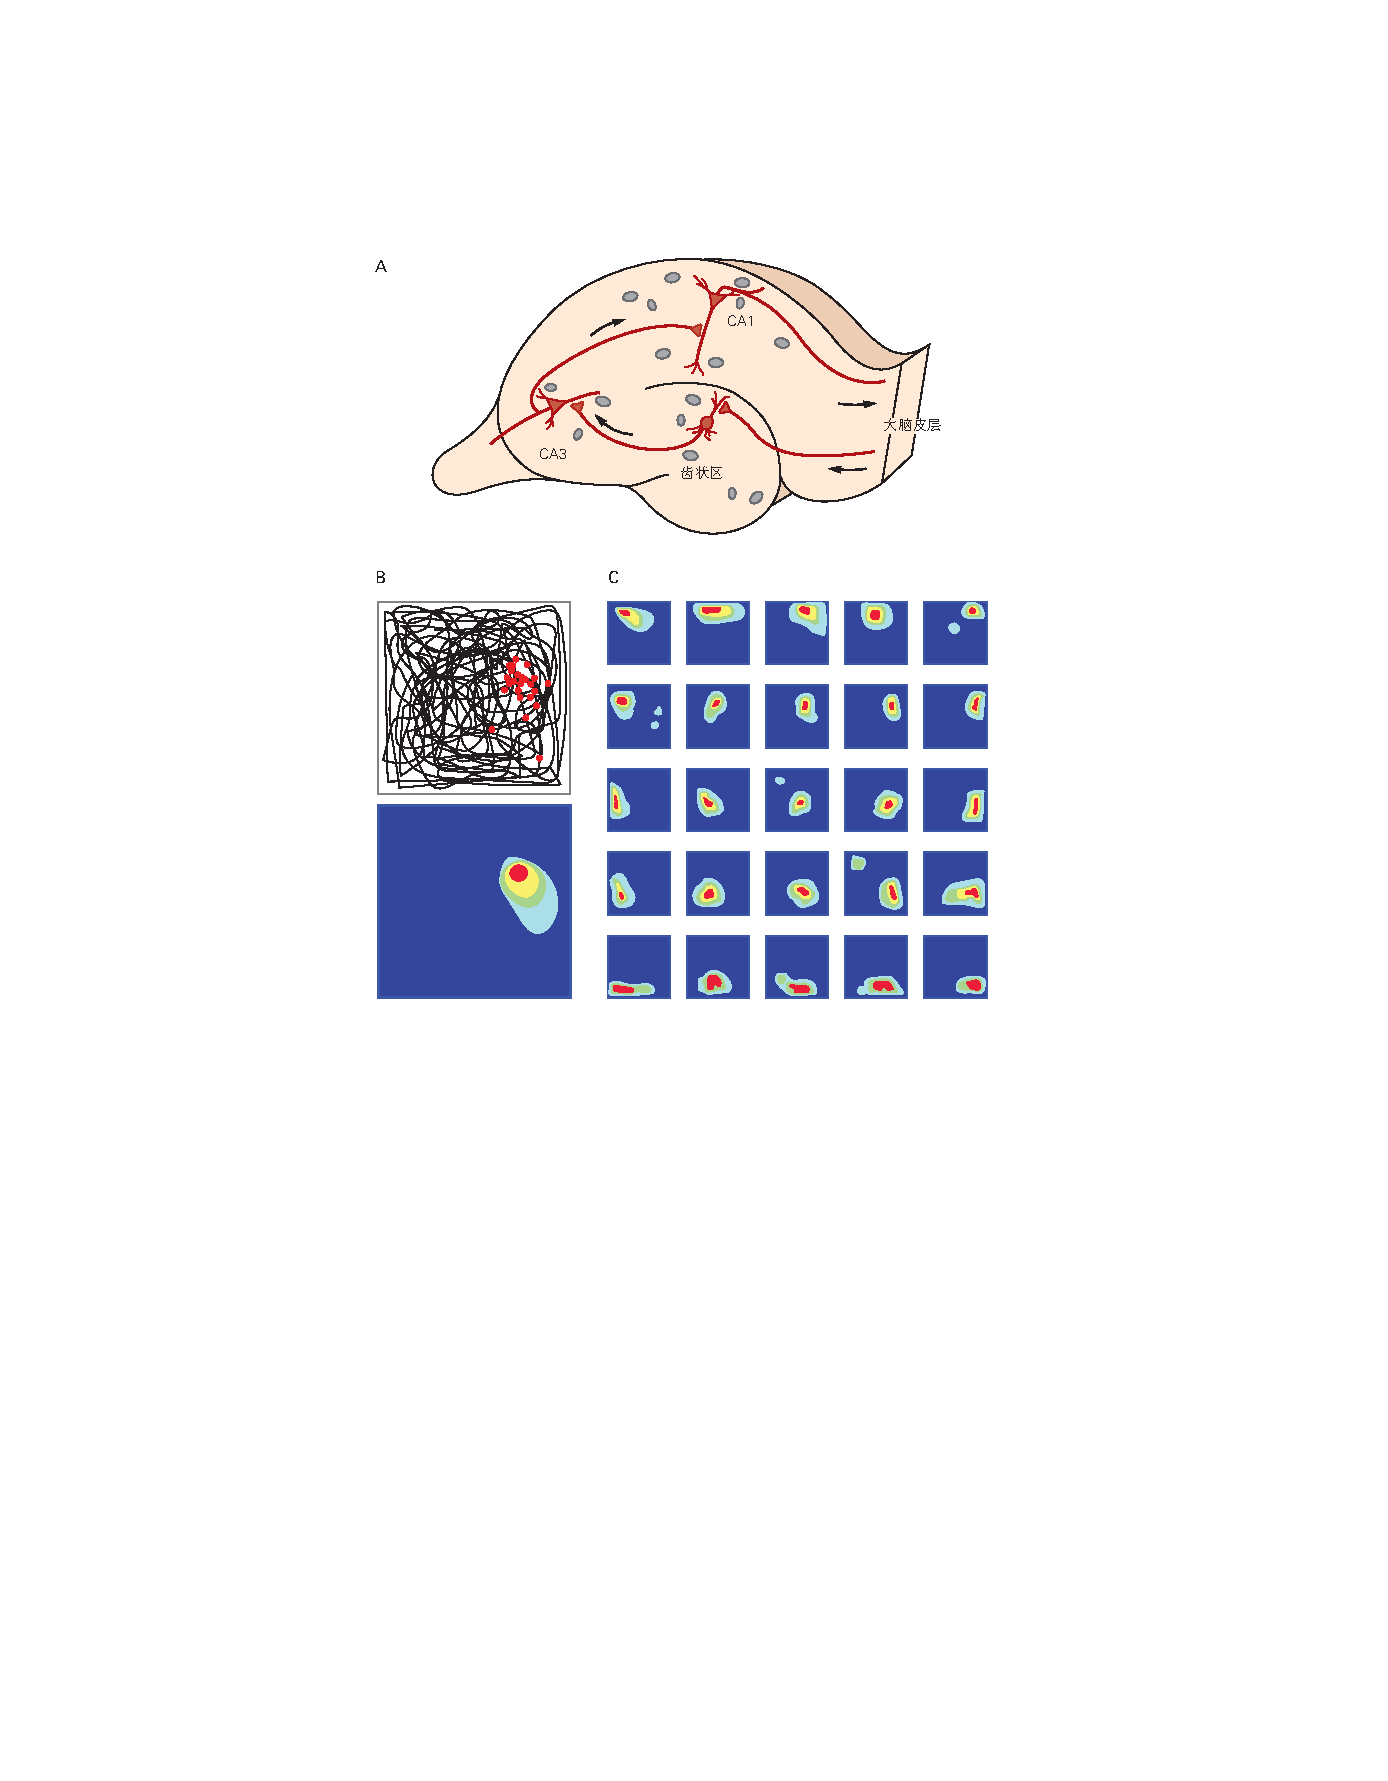
\includegraphics[width=0.9\linewidth]{chap05/fig_5_1}
	\caption{海马体位置细胞和位置细胞图。 
		\textbf{A.} 输入-输出转换发生在哺乳动物海马体的三突触回路中,从\textit{齿状回}输入区到\textit{阿蒙角}3 区,再到\textit{阿蒙角}1 输出区,每个区域的主要兴奋性神经元(红色)作为主要处理单元。
		主要细胞的活动由局部回路\textit{$\gamma$-氨基丁酸}活动的中间神经元(灰色)调节。
		\textbf{B.} 将细胞放电置于海马体中。
		老鼠穿过方形场地时所走的路径以黑色显示。
		电极被植入海马体内以记录单个细胞。
		上图:单个位置细胞会增加环境中离散位置的放电(每个动作电位由一个红点表示)。
		下图:位置细胞激活频率的颜色编码热图。
		较低波长的颜色(黄色和红色)代表在没有活动的背景(深蓝色)下较高的激活率。 
		\textbf{C.} 颜色编码的热图显示当大鼠探索一个方形盒子时在海马\textit{阿蒙角}1 区域同时记录的 25 个不同位置细胞的放电。}
	\label{fig:5_1}
\end{figure}


1971 年\textit{奥基夫}的可用的电生理方法仅限于一次记录一个位置细胞,但随后的进展允许研究人员同时记录数十个,最近数百个位置细胞。
关键的是,虽然单个位置细胞仅对环境的特定部分进行编码,并且容易在其位置场之外偶尔发出嘈杂的信号,但整个位置细胞群提供了更完整的空间覆盖和冗余位置编码的可靠性。
群体编码的这些特征为新的强大的计算分析铺平了道路。
特别是,可以解码位置细胞群体的活动并估计动物在环境中的位置。
这是通过确定每个细胞的空间选择性并使用该选择性作为模板来解码正在进行的活动来实现的。
在实践中,这种解码通常是通过加权每个细胞对动物位置最终估计的贡献来执行的,该因素与该细胞的空间编码可靠性成正比。
使用这种技术和类似技术,人们可以在房间大小的环境中以几厘米的精度逐秒重建动物的位置(图~\ref{fig:5_1}C)。



基于使用空间解码技术的研究,海马体功能与空间和陈述性记忆密切相关。
在积极探索环境期间,海马体活动反映位置编码,但在不动或静止行为期间,海马体进入不同的状态,在该状态下,神经活动由离散的半同步群体爆发主导,称为尖波涟漪(图~\ref{fig:5_2}A))。
这些事件被认为是由海马体内的回路在内部产生的。


\begin{figure}[htbp]
	\centering
	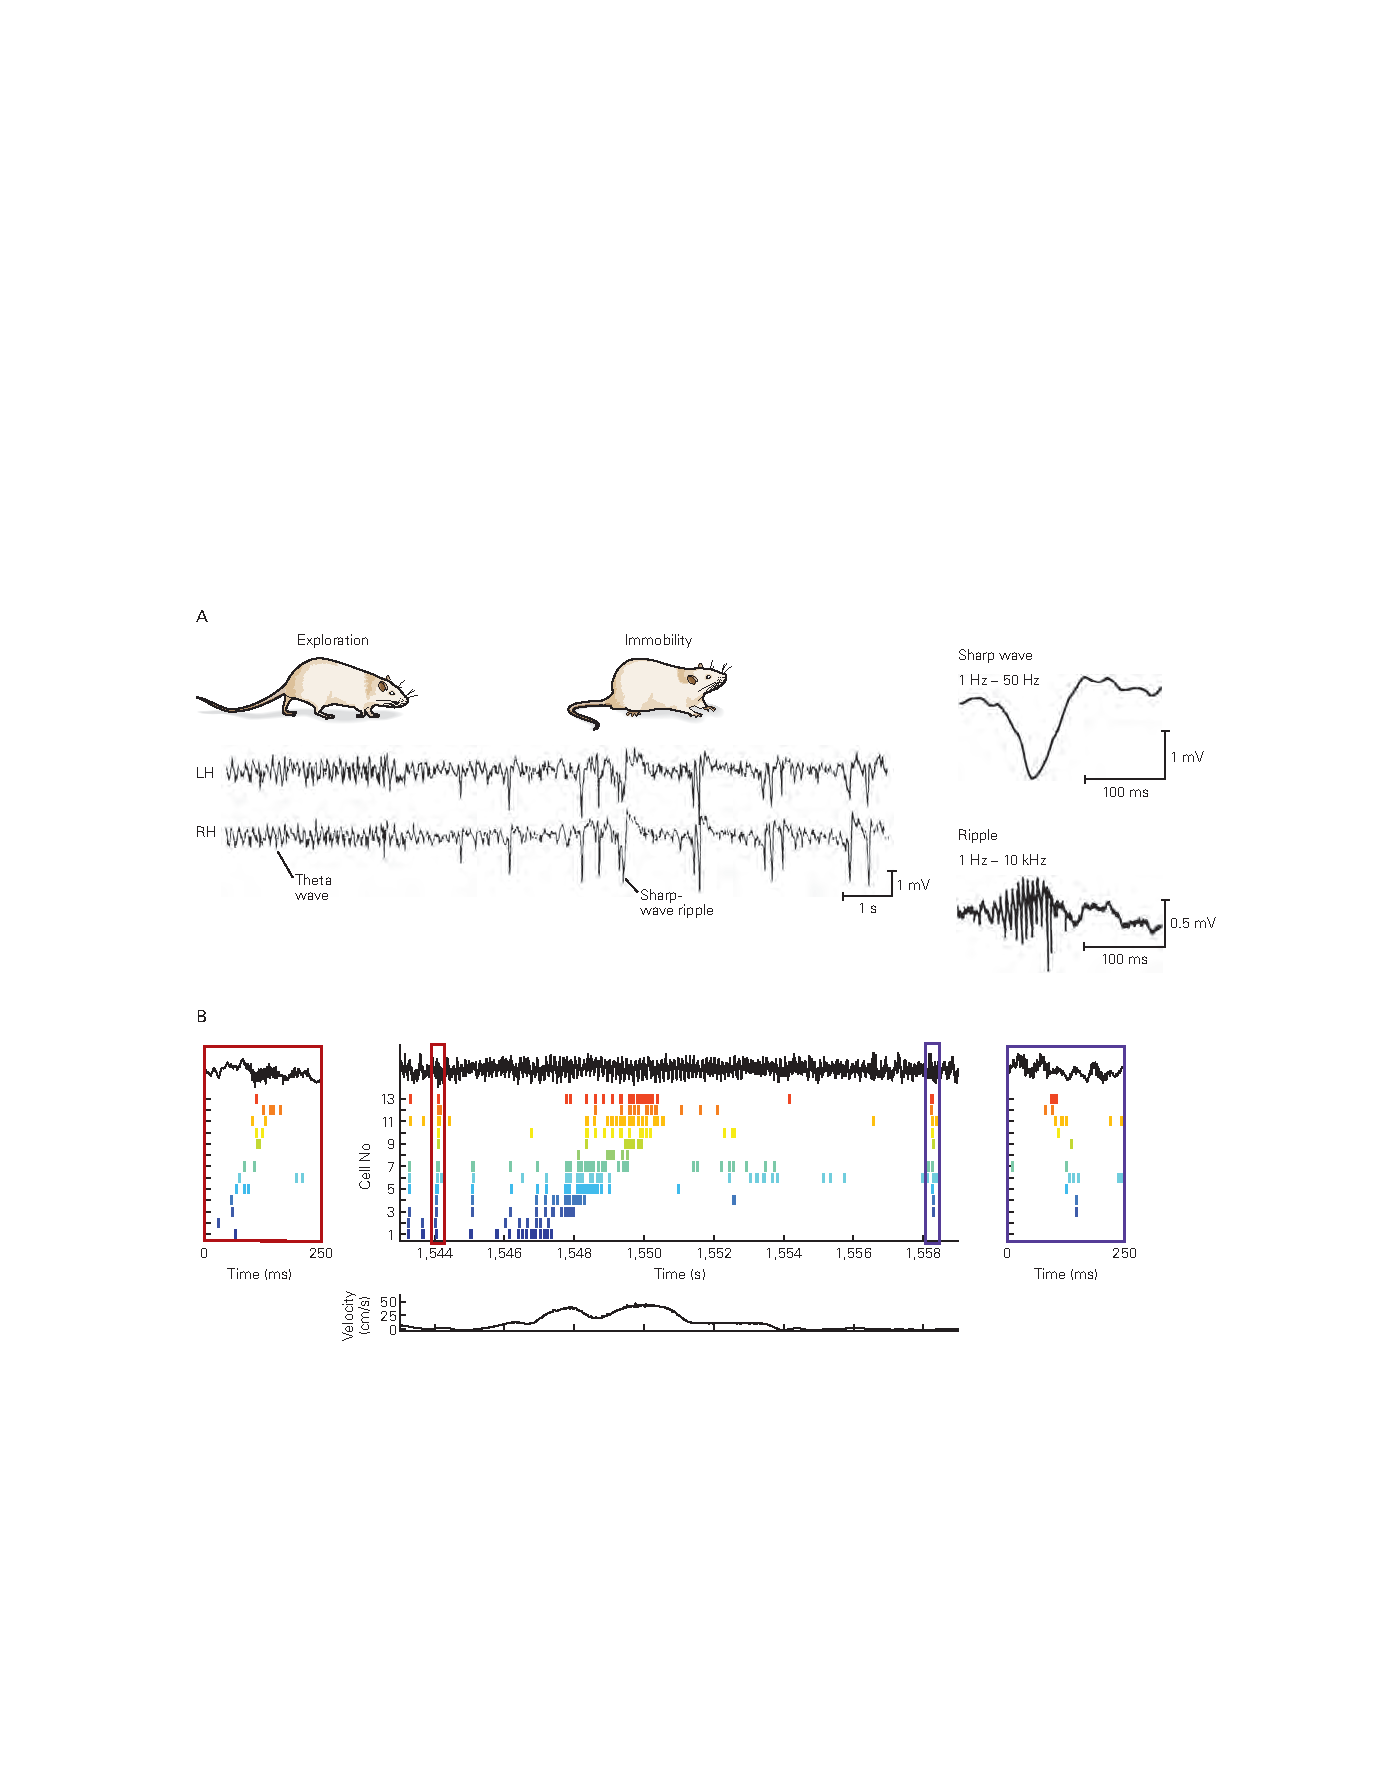
\includegraphics[width=1.0\linewidth]{chap05/fig_5_2}
	\caption{海马\textit{尖波涟漪}和\textit{序列回放}。 
		\textbf{A.} 左图:海马体\textit{局部场电位}活动的行为依赖性(\textit{左海马体}和\textit{右海马体})。
		在探索期间存在$\theta$波,在不动期间存在大的负尖波。 
		右图:从海马\textit{阿蒙角}1 区域记录的尖波和涟漪\cite{buzsaki2015hippocampal,buzsaki1992high}。
		\textbf{B.} 在行为(中图)期间经历的\textit{位置细胞}序列\textit{尖波涟漪}过程中在\textit{前向}(左图)和\textit{反向}(右图)方向上回放。
		老鼠沿着熟悉的轨迹从左向右移动。
		当大鼠在轨迹上时,13 个 \textit{阿蒙角}3 锥体细胞的位置场的脉冲序列显示在单次遍历之前(正向重放;红色框)、期间(中)和之后(反向重放;蓝色框)。
		\textit{阿蒙角}1 局部场电位显示在顶部(黑色痕迹),动物的速度显示在下方\cite{diba2007forward}。}
	\label{fig:5_2}
\end{figure}


值得注意的是,尖波涟漪在最近学习后的休息期间很突出,例如在探索环境之后,锐波涟漪很突出。
对在这些短尖波波纹内(50 毫秒到 500 毫秒)活跃的位置细胞活动的空间解码表明,海马神经元通过最近探索的环境重演或重播离散轨迹。
尽管这些轨迹复制了穿越空间的路径,但重播的活动序列在几个方面与主动探索期间观察到的不同。


首先,锐波波纹内的重放序列被时间压缩,发生速度比探索期间快 10 到 20 倍(图~\ref{fig:5_2}B)。 
其次,它们可以发生在与行为空间轨迹相同的方向(正向重播)或相反的方向(反向重播)。
因此,解码单个探索后的 200 毫秒尖波波纹重播事件可能会揭示一个虚拟的心理轨迹,该轨迹跨越 2 到 4 秒的行为时间,从它的经历中回放。
重放被认为代表了一种心理排练形式,通过这种形式,某些记忆逐渐得到巩固,因此可能是海马体在记忆中的作用的一个重要方面。



\section{神经回路基序为信息处理提供了基本逻辑}

神经元往往与附近的神经元和远端大脑区域的神经元高度互连。
由于许多揭示精细解剖结构的新方法,神经元连接的知识(称为连接组学)正在迅速扩展。
神经元互连的模式有多种。


从一个区域到另一个区域的连接,例如从丘脑到初级视觉皮层,被称为前馈(图~\ref{fig:5_3}A)。 
前向被定义为从更外围或主要区域(例如视网膜、丘脑或初级视觉皮层)延伸到具有更复杂响应特性的更高区域,例如选择性地响应特定目标的视觉区域。
在大多数情况下,具有前馈连接的两个区域也具有反馈连接。
例如,从初级视觉皮层到丘脑有许多连接。
局部连接通常从一个神经元延伸到另一个神经元,最终循环回到原始神经元。
这种循环连接称为循环。
许多神经元都参与了所有这些类型的连接(前馈、反馈和循环),但分开考虑这些不同连接基序的功能含义是有用的。


\begin{figure}[htbp]
	\centering
	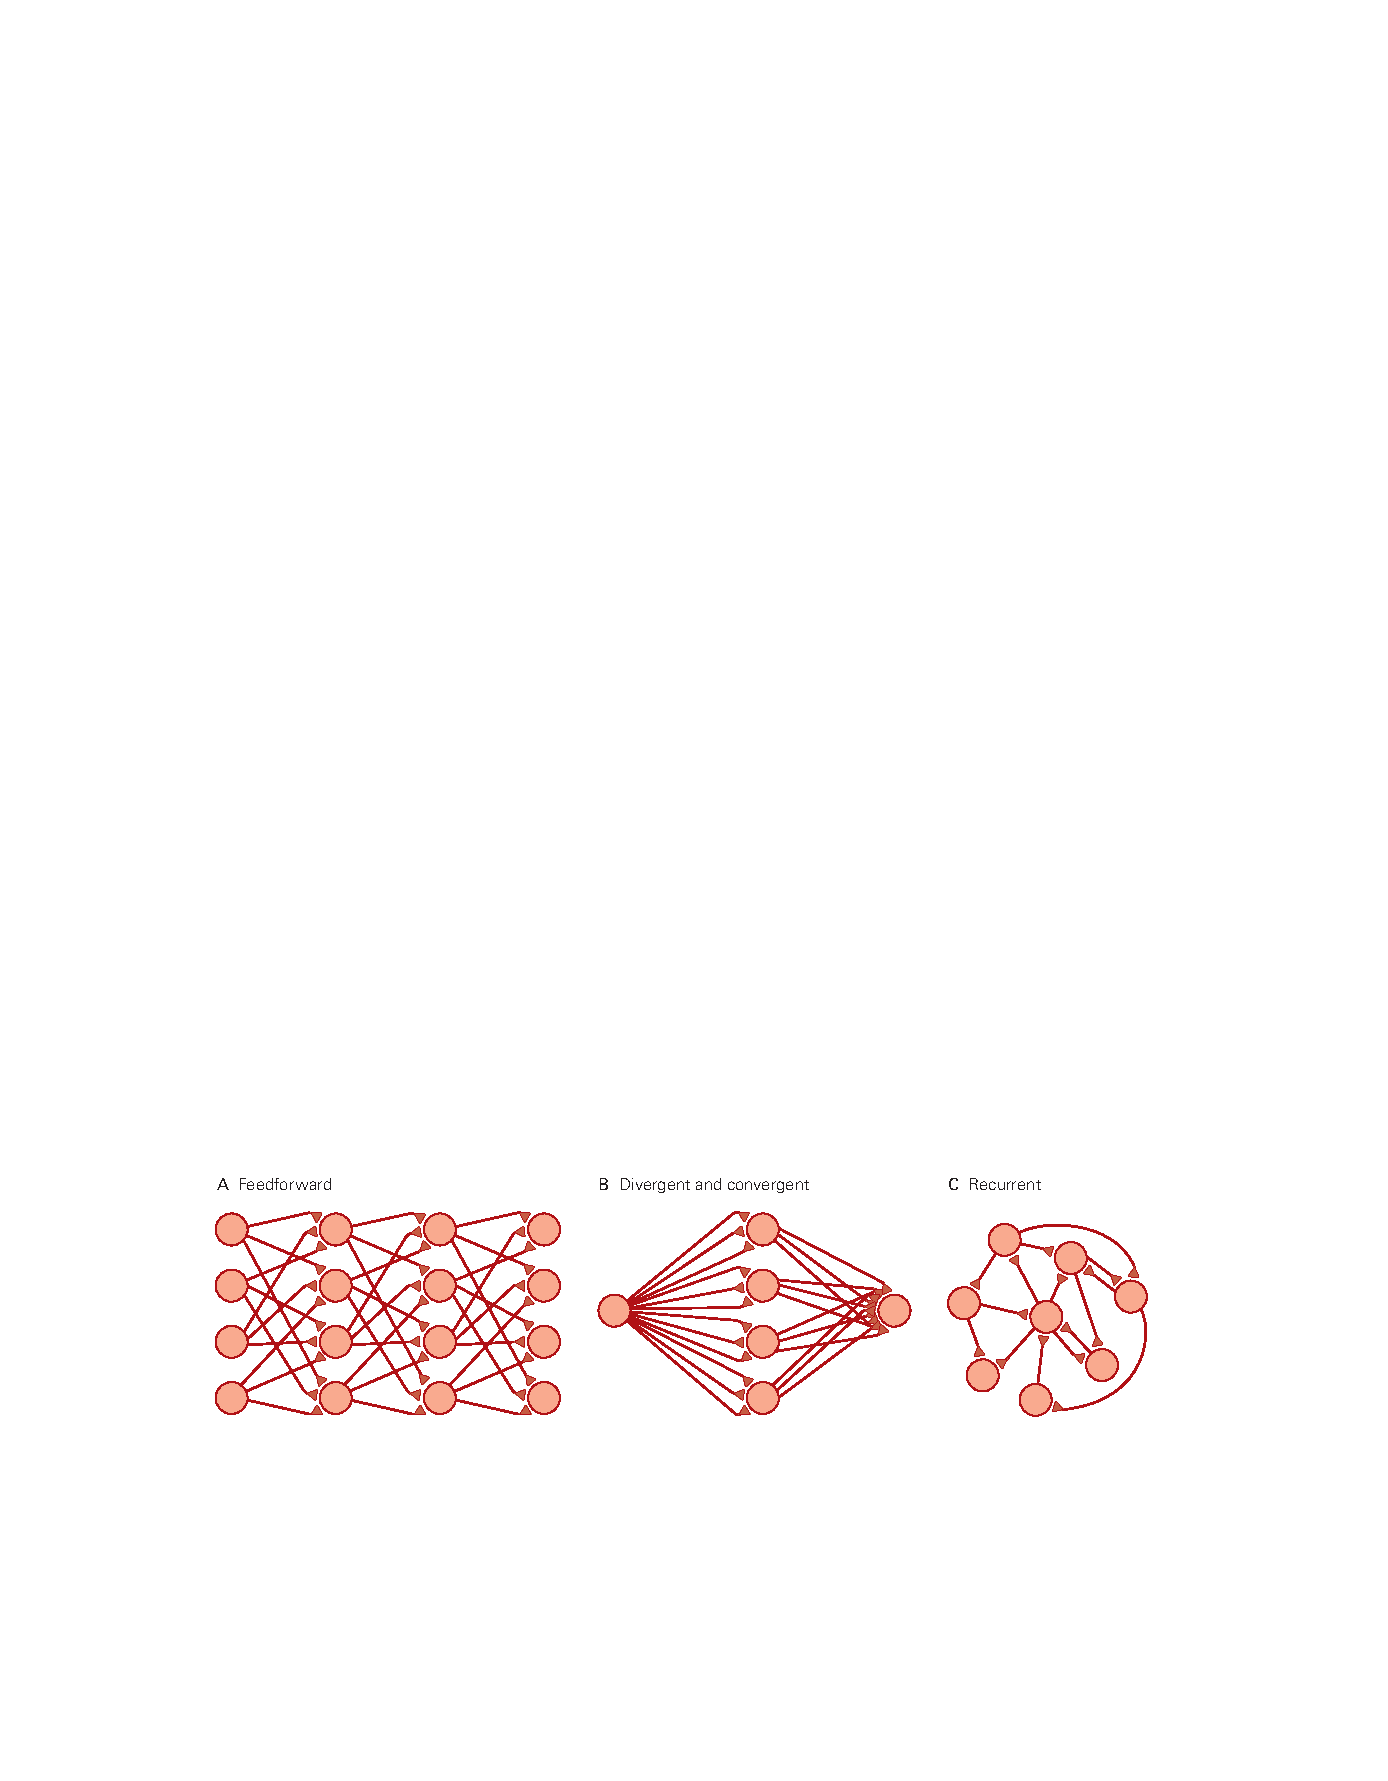
\includegraphics[width=1.0\linewidth]{chap05/fig_5_3}
	\caption{四种基本的神经回路图案。 
		\textbf{A.} 一种\textit{前馈}回路,其中突触连接在一个方向上从神经元的一个处理级别延伸到另一个处理级别。
		\textbf{B.} \textit{发散}的前馈连接描述了少量的突触前神经元连接到大量的神经元。
		\textit{汇聚}连接描述了连接到较小数量的大量突触前神经元。
		\textbf{C.} 在\textit{循环网络}中,神经元之间的多个方向发生突触连接,形成通过回路的循环通路。}
	\label{fig:5_3}
\end{figure}


神经元之间的连接可以是兴奋性的或抑制性的。
通常,兴奋性连接会导致神经放电增加,而抑制性连接会导致神经放电减少。
许多神经回路从成百上千个突触中接收到强烈的兴奋驱动。
如果不通过抑制来检查,这种突触兴奋将导致不稳定的神经活动。
兴奋和抑制的接近平衡是神经回路的一个共同特征,可以增强它们的计算能力。
然而,如果兴奋和抑制之间的平衡没有得到适当维持,这种微调可能会使回路容易产生癫痫发作活动,就像在癫痫期间发生的那样。


在哺乳动物中,视觉信息在一系列通常被近似为具有前馈回路的大脑区域中进行处理。
前馈回路可以以复杂的方式处理信息,例如从复杂的视觉场景中提取和识别目标,但它们不能产生持续的、动态的活动模式。
为此,需要循环回路(图~\ref{fig:5_3}C)。


在前馈回路中,可以识别两个子主题:发散连接和收敛连接(图~\ref{fig:5_3}B)。 
在发散连接中,接收给定类型输入的神经元数量超过提供该输入的神经元数量,因此在突触前输入神经元中编码的信息在突触后输出神经元中扩展。
在会聚连接中,许多突触前神经元将输入发送到数量较少的突触后神经元。
发散和收敛连接的最突出例子是由小脑提供的,如后所述。



\subsection{视觉处理和目标识别取决于前馈表示的层次结构}

视觉信息在大量分层排列的大脑区域中进行处理(图~\ref{fig:5_4})。
从视网膜产生的主要感觉输入向上移动,神经元对越来越复杂的视觉特征组合做出反应,最终导致对复杂物体(例如面部)的选择性。
大量研究致力于识别视觉层次结构所基于的原则。
机器视觉中人工神经网络模型的发展已被证明是解决该问题的一个有指导意义的类比。


\begin{figure}[htbp]
	\centering
	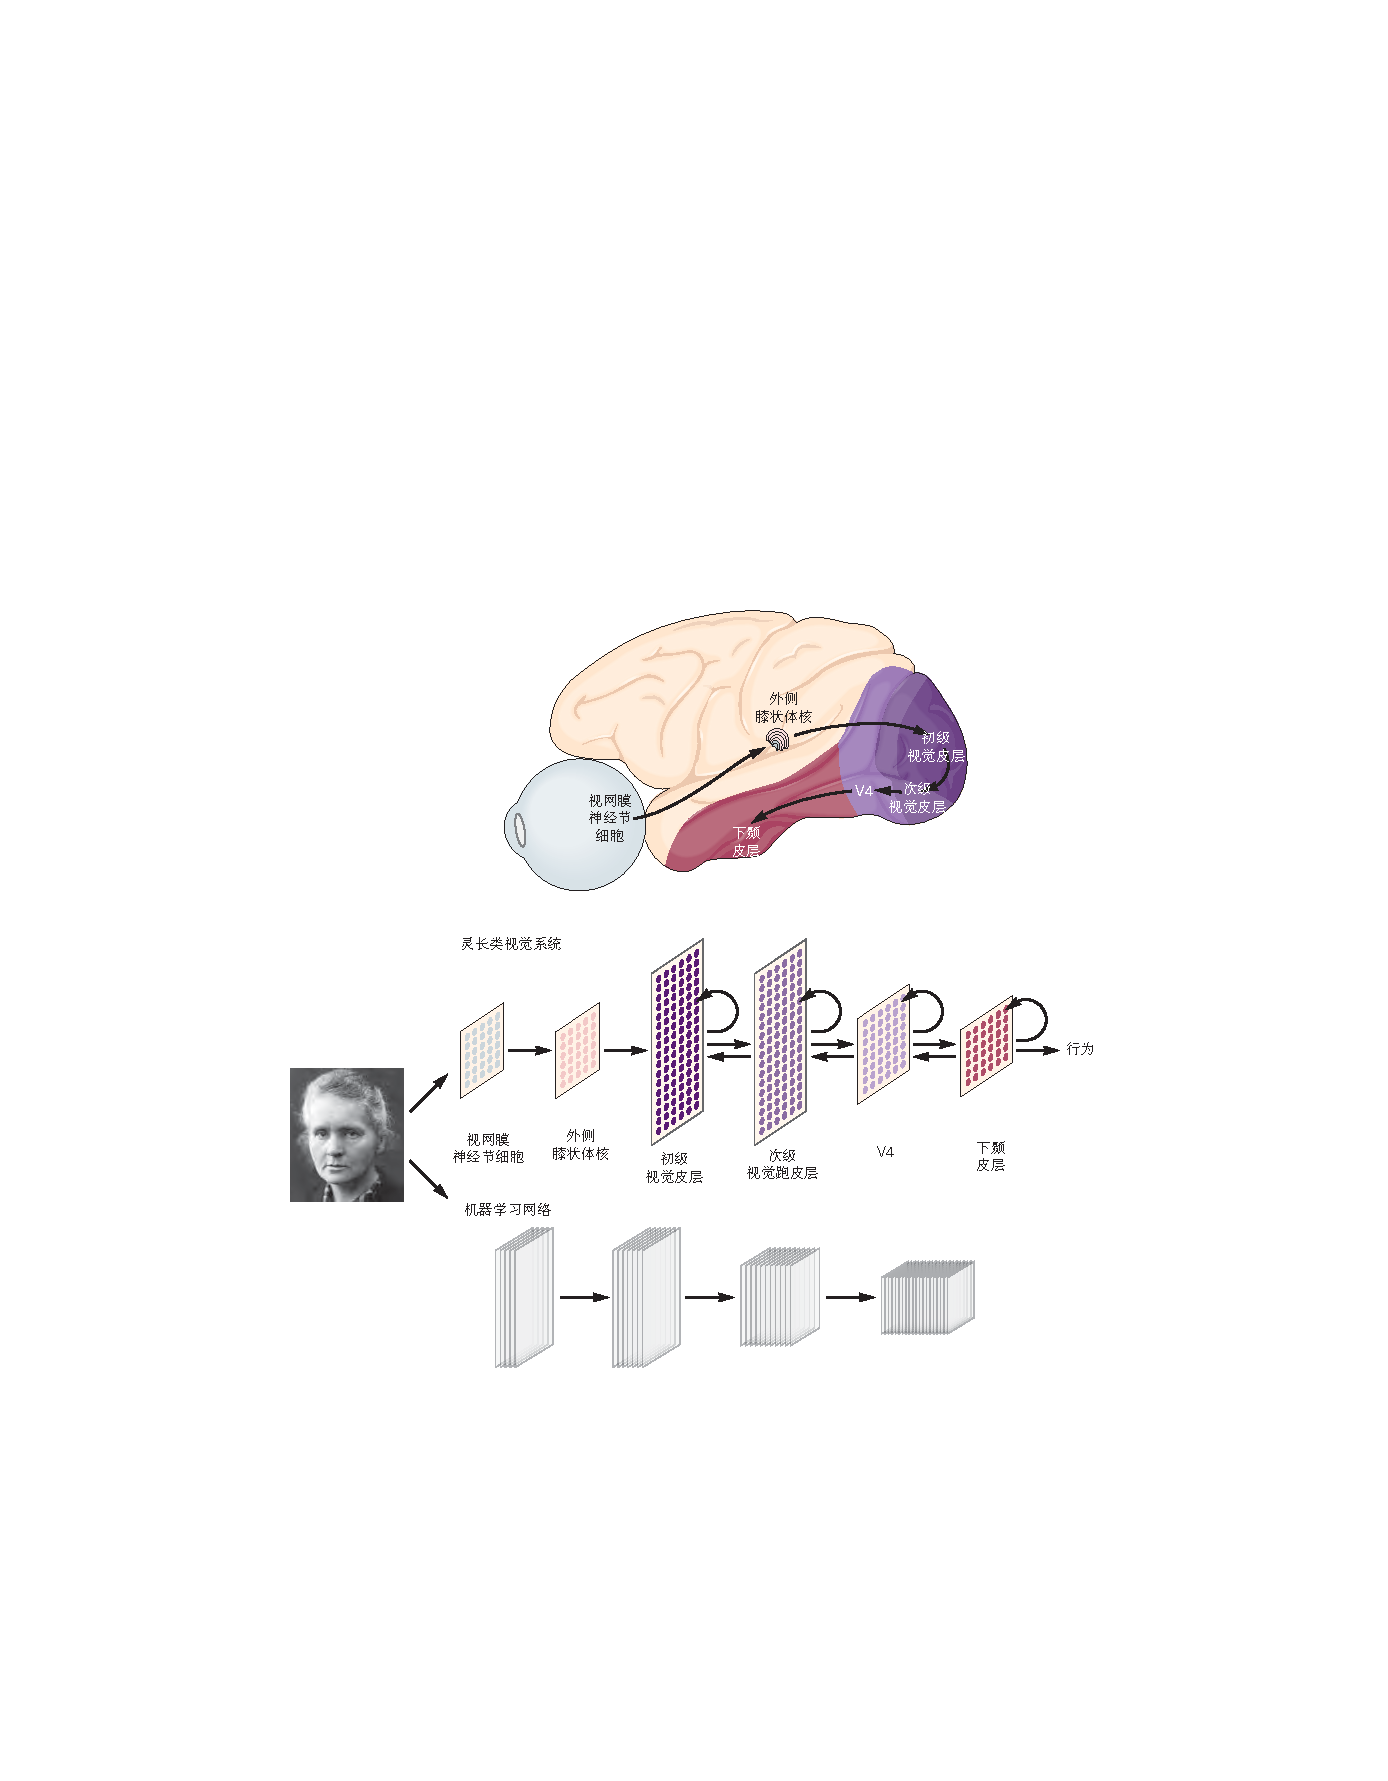
\includegraphics[width=1.0\linewidth]{chap05/fig_5_4}
	\caption{生物和机器学习网络的比较。
		在视觉系统中,多个大脑区域形成一个层次结构,在这个层次结构中,神经元逐渐对更复杂的物体进行选择。。
		灵长类视觉系统通路中的区域代表\textit{视网膜神经节细胞}、丘脑的\textit{外侧膝状体核}、腹侧流视觉区域(\textit{初级视觉皮层}、\textit{次级视觉皮层} 和 V4)和\textit{下颞皮层}。
		每个区域的神经元\textit{数量}各不相同(由彩色圆点表示),但它们的\textit{选择性}稳步增加。
		机器学习网络通路表示经过训练以识别图像中目标的前馈网络层。
		越来越多的堆叠子层表明机器学习网络不同区域的选择性增加,反映了对更丰富的视觉特征阵列的选择性。
		在不同视觉区域记录的响应选择性的层次结构类似于在机器学习网络的相应层中看到的活动\cite{schrimpf2018brain}。}
	\label{fig:5_4}
\end{figure}



从视网膜到丘脑,再到初级视觉皮层,再到与认知相关的最高视觉区域下颞皮层中,视觉神经元选择性地响应视野区域中特定的亮、暗和颜色模式,称为它们的\textit{感受野}。
从视觉处理的最低阶段到最高阶段,神经元的感受野越来越大,选择性也越来越高。
在每个阶段,具有特定类型选择性的神经元往往倾向于具有覆盖视觉场景的感受野,为所选特征提供全面覆盖。
此外,每个视觉大脑区域中感受野的排列在地形上与视网膜上外部世界图像的布局相匹配,即皮层形成了视野图。


随着感受野的扩大和选择性的增加,神经响应对所选目标或图案精确位置的依赖程度越来越低,而更多地取决于其整体特征。
一般来说,处于视觉处理较高阶段的神经元对视野的较大部分更有选择性地做出反应,并且较少依赖于位置、大小和方向等特征。
这与我们在场景中独立于位置、大小和方向识别目标的能力相关。
例如,在层次结构的最高阶段,神经元可以选择性地对位于中间的特定面孔做出反应,而与面孔的大小或其角度姿势(即头部方向)无关。


平铺、增加感受野大小、增加选择性和减少对视图相关因素的依赖的想法是人工机器视觉网络构建的核心。
这样的网络在某些物体识别任务上可以达到人类水平的性能。
此外,机器在困难图像上所犯的错误模式在某种程度上与人类受试者所犯的错误相匹配。
非人类灵长类动物也可以在与人类相当的水平上执行这些任务,而且有趣的是,沿着目标识别通路的不同视觉区域的记录对应于在视觉处理的相似阶段在人工网络中看到的活动(图~\ref{fig:5_4})。



\subsection{小脑中不同的神经元表征为学习提供了基础}

我们大脑中最丰富的一类神经元是位于小脑输入阶段的大约 500 亿个颗粒细胞,占大脑所有神经元的一半以上。 
小脑是一种对运动协调至关重要的后脑结构,但也涉及自主神经、感觉和认知功能的适应性调节(图~\ref{fig:5_5})。
小脑回路功能障碍可能导致各种神经系统疾病,包括孤独症。
与大多数大脑神经元接收的数千个输入相比,每个颗粒细胞仅接收少量输入(平均四个)。


\begin{figure}[htbp]
	\centering
	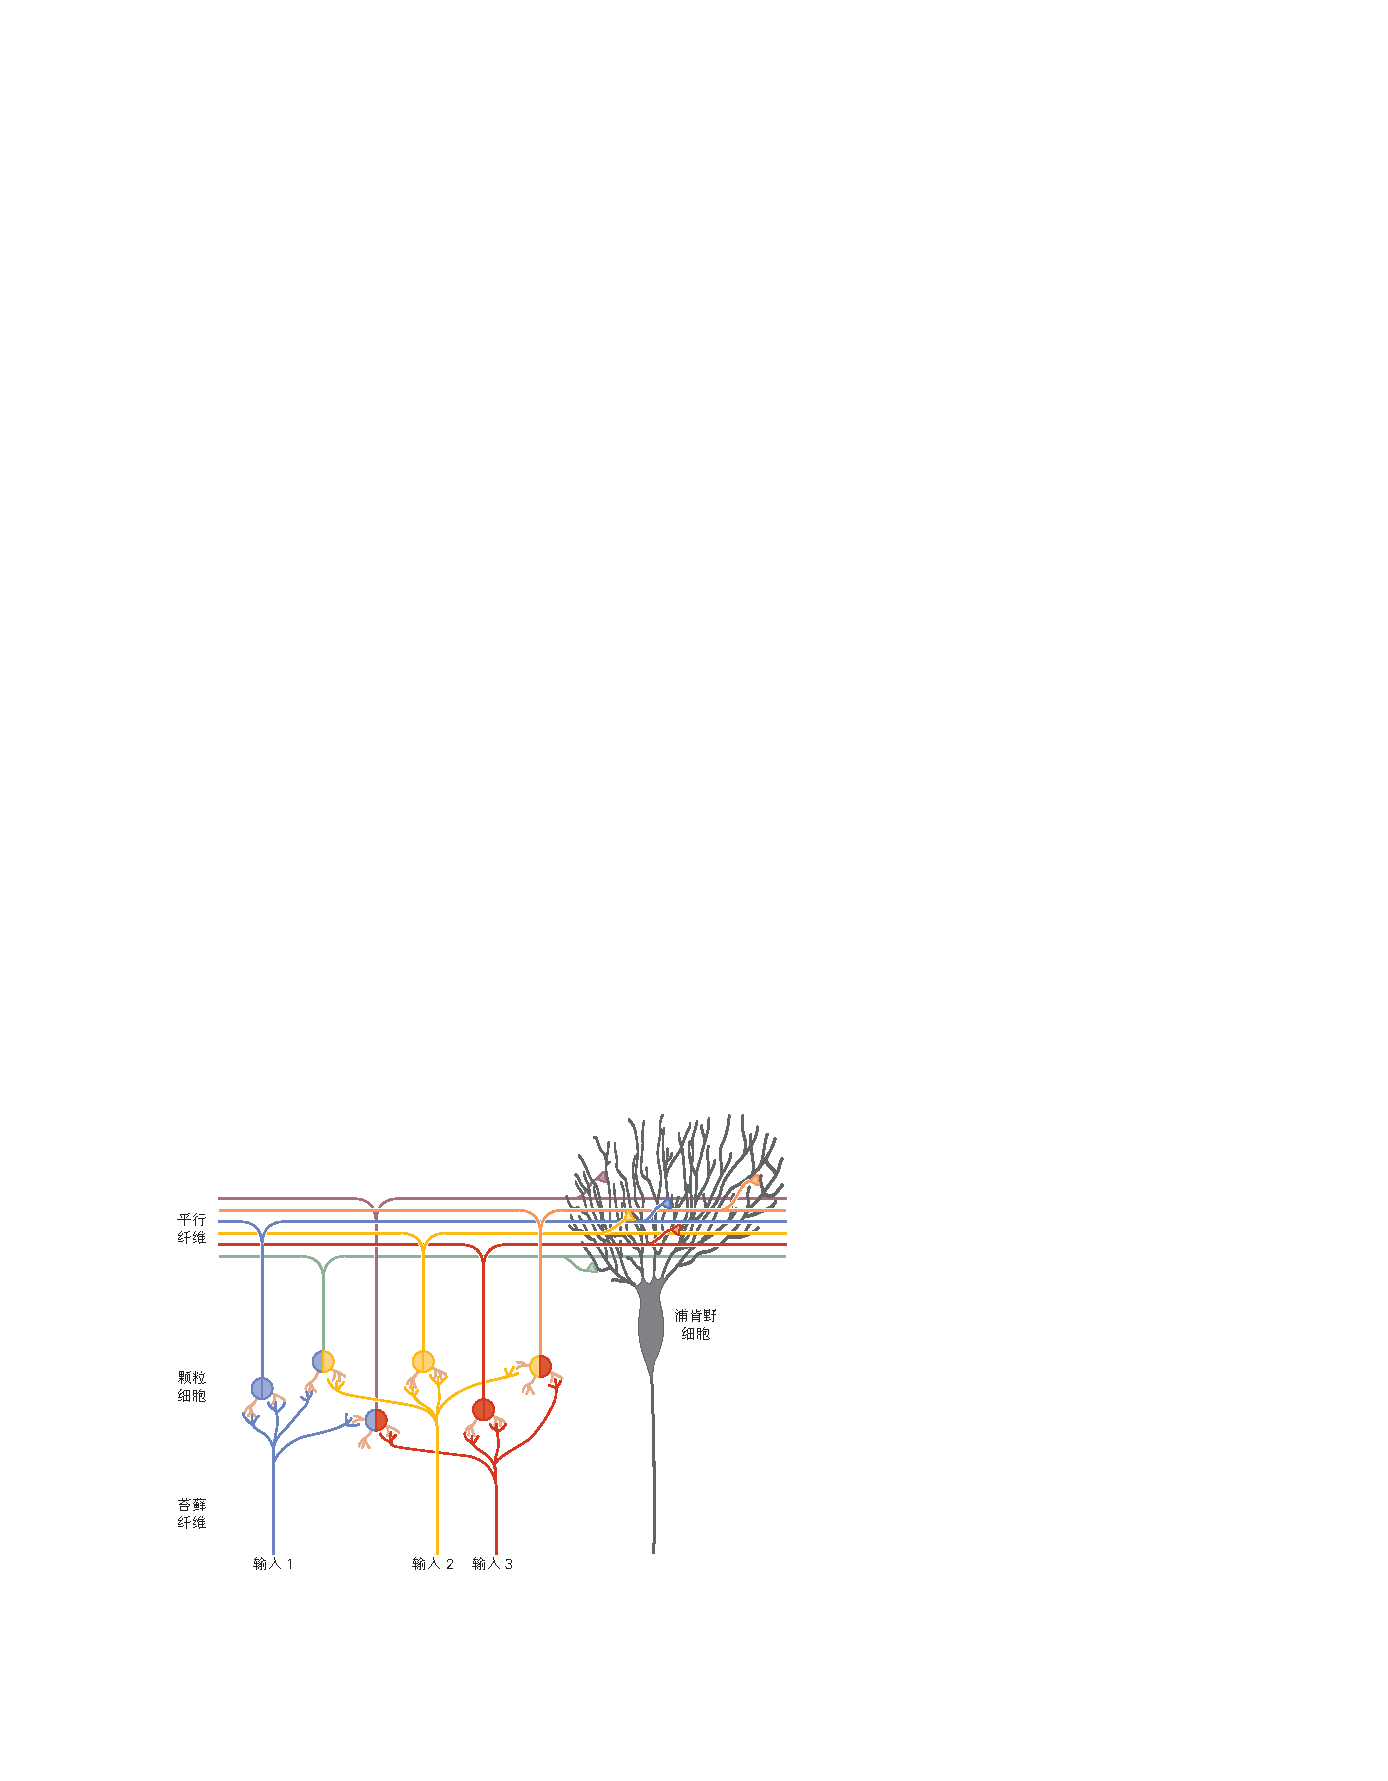
\includegraphics[width=0.9\linewidth]{chap05/fig_5_5}
	\caption{小脑接收来自大脑和脊髓许多区域的输入。
		这些输入统称为\textit{苔藓纤维},在大量\textit{颗粒细胞}中重新编码,这是发散连接的一个例子,允许输入信号的许多可能混合。
		\textit{浦肯野细胞}的树突从轴突(称为平行纤维)中继的数十万个颗粒细胞接收会聚输入。
		浦肯野细胞突触的平行纤维是可改变的,这被认为是运动和可能其他形式学习的重要机制。}
	\label{fig:5_5}
\end{figure}


最近使用神经解剖学追踪和电生理学记录的实验结果表明,汇聚到单个颗粒细胞上的输入通常来自不同的大脑区域。
因此,单个颗粒细胞的放电可能代表大量刺激或事件组合中的任何一种。
例如,细胞可能仅在特定视觉刺激(例如移动的网球)与特定身体部位的运动(例如手腕的弯曲)结合时才会放电。
以这种方式组合不同类型信息的表示称为混合表示。


小脑颗粒细胞提供了\textit{发散前馈连接}的一个极端例子,大约 2 亿个输入纤维(称为\textit{苔藓纤维})携带的信息混合并扩展到 500 亿个\textit{颗粒细胞}上。
需要如此大的表示来处理可以组合多个信息通道的许多不同方式。
例如,表示 100 个不同输入通道中的 2 个的所有可能组合需要 100 × 99/2,即 4,950 种不同的响应类型。
需要所有三元组的表示将这个数字推高到 15 万以上,并且对于四个或更多的组合,这个数字会迅速增加。
由于大量可能的组合在遗传学上很难确定,所以通常认为苔藓纤维与其颗粒细胞目标的分配在很大程度上是随机的。


该分析表明,小脑颗粒细胞的作用是以多种可能的方式\textit{组合}大量输入通道。
这种表示显然有助于根据刺激和动作组合的共现进行推理和生成动作。
然而,要发挥作用,必须以某种方式从大量颗粒细胞中读出这些信息。


小脑细胞的\textit{读出}是由浦肯野细胞完成的,浦肯野细胞是小脑皮层的输出神经元。
与颗粒细胞输入端高度分散的连接相反,颗粒细胞和浦肯野细胞之间的连接提供了一个极端的\textit{汇聚}例子。
单个浦肯野细胞接收来自超过十万个颗粒细胞的输入。
\textit{大卫$\cdot$马尔}和\textit{詹姆斯$\cdot$阿尔布斯}在 1970 年代提出的小脑功能理论认为,这种融合使\textit{浦肯野细胞}能够从颗粒细胞提供的极其丰富的表征中提取有用的信息。
通过这样做,浦肯野细胞可能是人类形成运动技能(如骑自行车或演奏乐器)所需的许多复杂联想的惊人能力的基础。
然而,为了在各种条件下提取对多种目的有用的信息,浦肯野细胞提供的读数必须具有适应性。
如后面部分所述,这种适应性是由颗粒细胞和浦肯野细胞突触之间的\textit{突触可塑性}提供的。



\subsection{循环回路是持续活动和整合的基础}

神经元天生健忘。 
瞬态突触输入通常会引起短暂的响应,这种响应会在几十毫秒内衰减。
这种衰变的时间过程由神经元的一种内在特性决定,称为\textit{膜时间常数}(第~\ref{chap:chap9}~章)。
那么神经活动模式如何持续足够长的时间以支持认知操作,例如在几秒钟、几分钟甚至更长时间内完成记忆或决策制定?


例如,试着在一个挤满人大声说话的房间里尝试检测您是否听到一个熟悉的声音。
当您聆听时,您可能偶尔会发现一些类似于您正在寻找的声音,但这本身并不能确定。
然而,随着时间的推移,您可能会积累足够的证据来得出结论。
这个证据积累的过程需要整合,这意味着必须维护一个运行总和,并在检测到额外证据时增加。
整合需要计算(加法)和记忆来计算和维护运行总和(第~\ref{chap:chap56} 章)。


为了使神经回路进行整合,瞬态输入必须产生即使在输入消失后也能维持在恒定水平的活动。
这种持续的活动提供了对瞬态输入的记忆。
如前一段所述,整合的神经回路可用于积累信息,但它们也需要用于非认知任务,例如保持固定身体姿势所需的恒定肌肉张力。
研究得最好的神经整合器之一是允许人类和动物保持眼睛恒定注视方向的回路,即使在黑暗中也是如此。
事实上,可以研究从鱼类到灵长类动物广泛物种的眼球运动,这极大地促进了研究的进步。
此外,动眼神经系统的相对简单性促进了实验研究和理论研究之间富有成效的对话(动眼神经系统在第~\ref{chap:chap35} 章有更详细的描述)。


动眼神经系统中整合回路的存在最初是由来自神经元记录的一个令人费解的观察结果提出的(图~\ref{fig:5_6}A)。
控制眼部肌肉的动眼神经元会瞬时增加动作电位放电以引起眼睛的运动,但也会表现出将眼睛保持在固定位置所需的持续动作电位放电。
例如,当注视保持在中心的左侧时,投射到眼球肌肉的运动神经元的放电频率高,而当注视保持在中心的右侧时,放电频率低。
令人困惑的是,投射到动眼神经元的上丘和脑干中的运动前神经元仅在眼球运动之前短暂放电。
他们没有表现出任何与眼睛位置相关的持续活动。
那么这种持续的活动是如何产生的呢?


\begin{figure}[htbp]
	\centering
	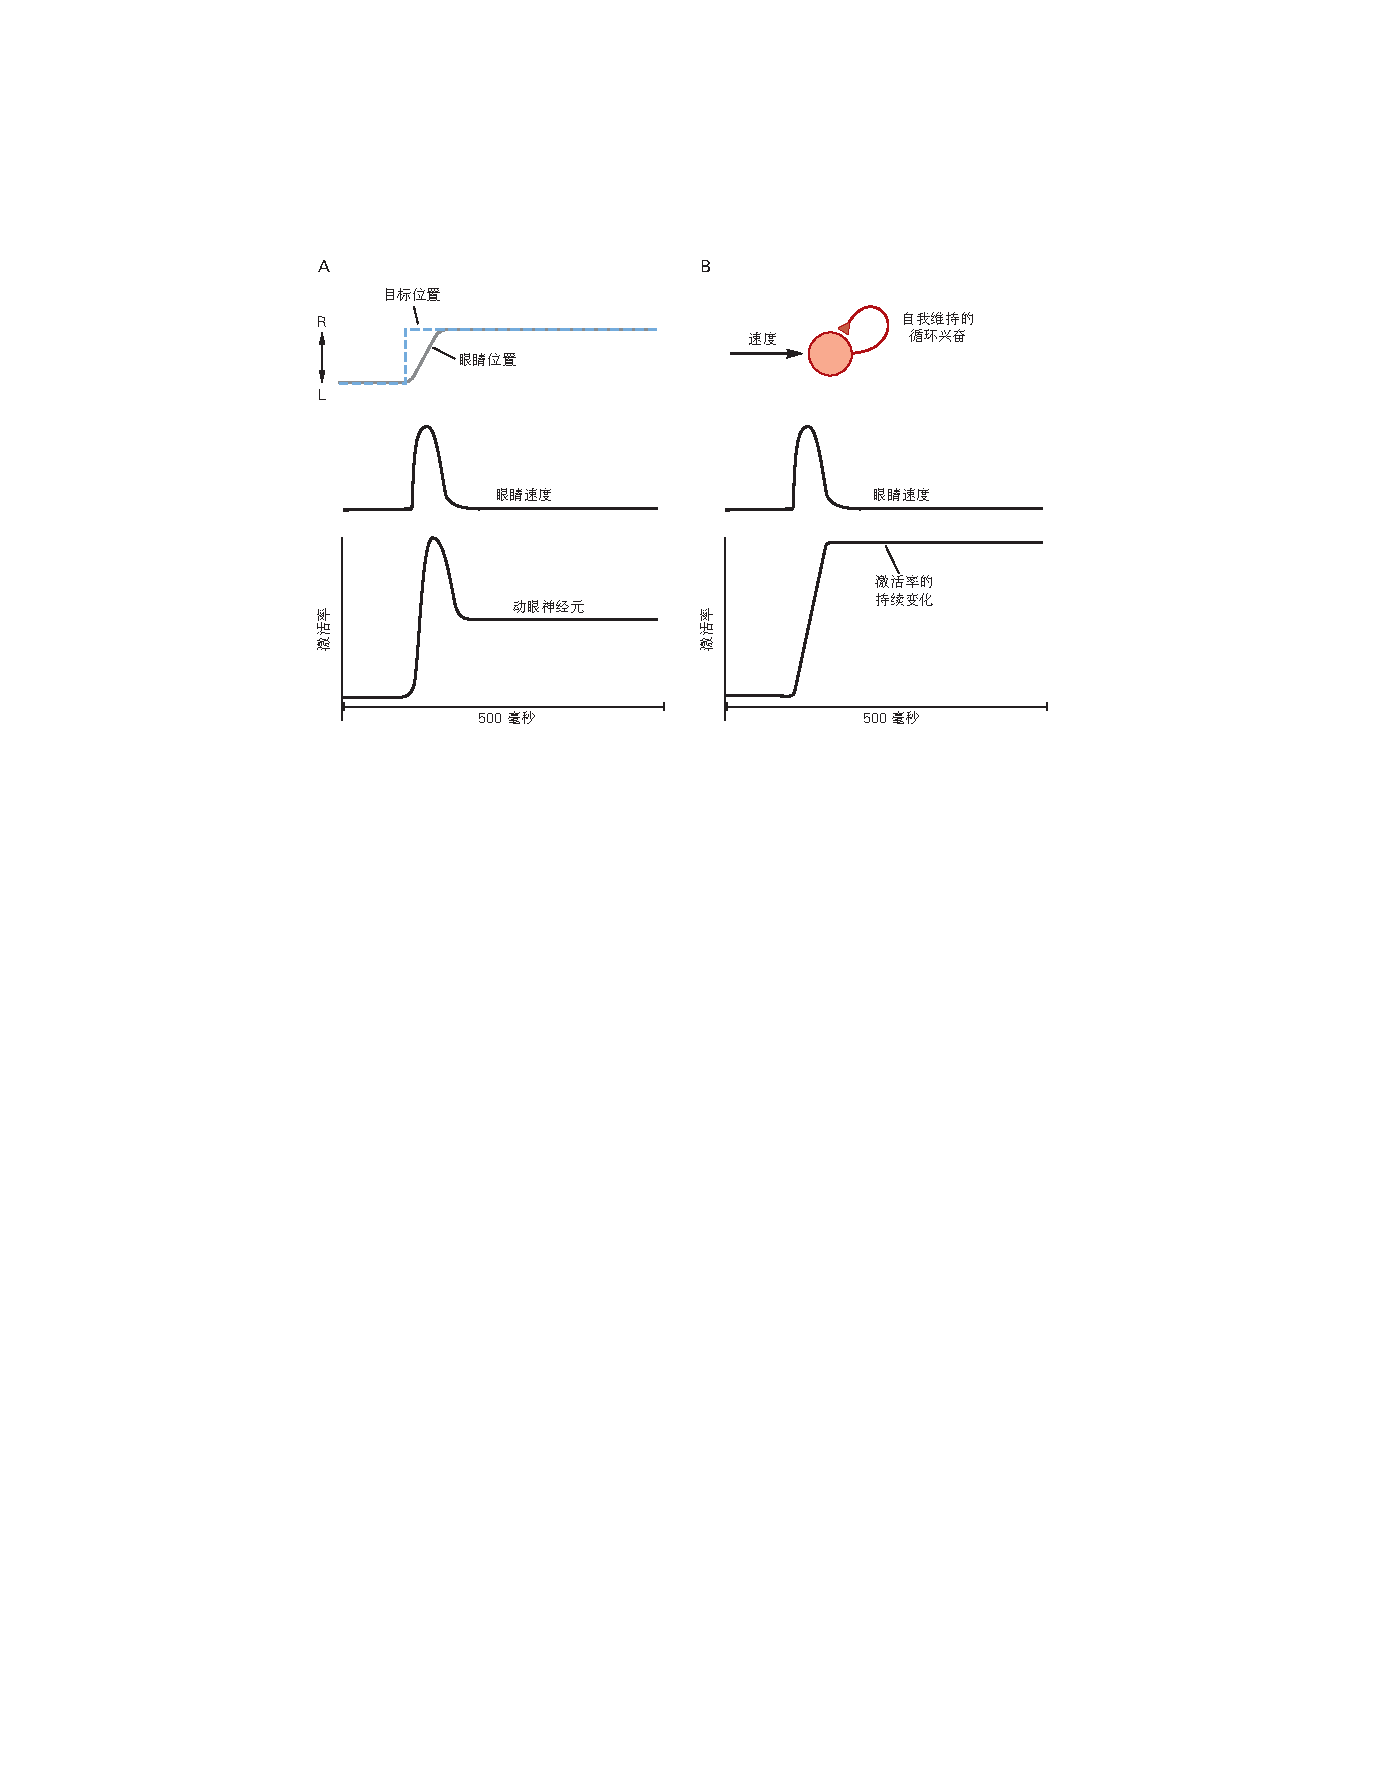
\includegraphics[width=0.9\linewidth]{chap05/fig_5_6}
	\caption{维持眼睛位置需要循环回路和持续的神经活动。
		\textbf{A.} 上图:一个\textit{扫视}的眼球运动包括眼球速度的快速运动变化,以将目标带回凝视中心。
		随后持续改变眼睛位置以将中央凹保持在目标上。
		蓝色虚线表示\textit{目标位置},灰色线表示眼球运动和随后在新位置对目标的注视。
		下图:动眼神经元表现出与眼睛速度相关的短暂活动以及与眼睛位置相关的持续活动。
		\textbf{B.} 反复的兴奋可以解释一个短暂的脉冲输入(例如眼速信号),是如何通过类似于数学积分的过程导致放电率的持续变化。}
	\label{fig:5_6}
\end{figure}


一个早期的猜想,现在得到了强有力的支持,即稳定的眼睛位置信号是由脑干神经元计算的,整合了瞬态眼速度信号。
这些神经元接收速度信息并向维持眼睛位置的动眼神经元提供稳定的输出。 
猴子某些脑干核团(包括内侧前庭核和舌下舌前核)的损伤或失活导致眼球运动后无法保持稳定的水平眼位,表明神经整合回路位于这些结构内。 
人类这些脑干结构的损伤会导致同样的问题,临床上称为凝视诱发性眼球震颤(第~\ref{chap:chap35}~章)。


神经回路如何进行整合?
一种可能性是整合得到专门内在神经元特性的支持,这些特性有效地延长了神经元\textit{膜时间常数},允许短暂的输入产生持续的输出。
已经描述了涉及不同电压激活离子通道的多种候选机制。 
然而,使用允许直接控制记录神经元的膜电压的细胞内记录的研究表明,即使神经元的电压激活通道被阻断,持续的位置相关信号也会持续存在。 
第二种可能性是整合源于突触耦合神经元网络之间的相互作用。 
金鱼的细胞内记录支持这一观点,显示突触输入水平随着眼睛位置的变化而变化。


什么类型的神经网络能够执行整合的问题已经在理论研究中得到广泛探索。 
已考虑的一类模型依赖于循环连接,特别是一群相互激发的神经元。 
这种类型的弱耦合网络响应具有快速衰减的活度的输入脉冲。
增加反复激发的强度会增加一些原本会衰减的活动,从而延长群体反应的持续时间。
如果循环激励增加到由瞬态输入建立的循环激励精确抵消衰减的程度,则响应可以无限期地持续。 这需要微调网络参数。


在一个完美调谐的网络中,一个瞬态输入脉冲会导致激活率发生变化,这种变化在没有进一步输入的情况下会永远持续下去。 
等效地,这样的群体计算它接收到的输入的运行整合(图~\ref{fig:5_6}B)。
如果网络中的瞬态激励没有得到完美调整,则输入会产生放电速率的变化,并且衰减缓慢。 
在黑暗中,眼睛位置往往会在大约 20 秒内漂移回中心,这表明神经整合器没有被完美地调整,但当它被调整得足够好时,可以将典型神经元的大约 20 毫秒时间常数延长一个约1000的系数。


循环网络模型再现了在生物整合器回路中观察到的一些核心特性这一事实已经启动了更详细和更现实的网络模型的开发,并通过实验测试了此类模型的预测。
这些努力还突出了在神经回路的结构和功能之间建立详细联系所涉及的挑战。
即使在使用各种系统和方法进行了数十年的深入研究之后,关键问题仍然存在。


例如,动眼神经整合器回路通常包含两类相反的神经元,随着眼睛位置在给定方向上的变化,一类神经元的放电率增加,另一类神经元的放电率降低。 
这种排列不仅限于动眼神经整合器,而且在涉及决策和工作记忆的皮质区域也发现了这种排列。
模型表明,这些对立群体之间的相互抑制可以在维持活动和融合方面发挥作用。 
尽管解剖学研究为这一观点提供了一些支持,但对金鱼的研究表明,即使对立群体之间的联系被移除,整合仍然完好无损。


另一个关键问题涉及调整积分器网络的机制。
实验研究表明,整合器网络可以根据经验进行修改。
换句话说,它们是可调的。 
尽管这种调整可能是通过神经元之间突触连接强度的变化而发生的,但尚未获得直接证据。 
简而言之,尽管已经了解了很多关于如何实现集成的知识,但在任何特定实例中实际支持集成的网络架构的细节仍有待确定。


详细了解我们如何保持眼睛的位置本身就是一个重要的目的,具有临床意义。 
然而,如前所述,此处找到的解决方案可能同样适用于认知功能,包括短期记忆和决策制定。
大量神经元的光学成像以及对其活动的时间精确操作和详细的解剖学重建,再加上网络功能的理论模型,可能很快就会提供答案。



\section{学习和记忆取决于突触可塑性}

经验可以改变神经回路以支持记忆和学习(第~\ref{chap:chap3}~章)。
一般认为,负责学习和记忆的经验依赖性变化主要发生在突触上。
已经确定了多种形式的突触可塑性,其中每一种都可能支持一组不同的功能。


正如可塑性有多种形式一样,学习也有多种形式。
可以根据所提供信息的数量和类型来定义不同的学习形式。
在监督学习中,会给出有关执行任务所需行为的明确指示。
另一方面,在强化学习中,仅提供正奖励或负惩罚来指示该任务是否被正确执行。
最后,无监督学习根本不涉及任何指导性信息,而是在没有监督的情况下,根据输入数据的内在结构对其进行组织。
在以下部分中,我们将讨论涉及赫布可塑性的无监督学习示例和小脑强化学习示例(学习和记忆的各种类型及其细胞和回路机制在第~\ref{chap:chap52}~至~\ref{chap:chap54}~章中有详细描述)。



\subsection{突触输入的主导模式可以通过赫布可塑性来识别}

皮层神经元接收来自数千个其他神经元的突触输入,并将这些信息组合成动作电位模式。
每个突触的突触传输强度决定了来自许多输入的信息如何组合以影响神经元的放电。
将所有突触的强度设置为零,显然会使无信息的神经元失去功能。
同样,将它们设置为非零值以提取由随机噪声主导的信号也不会产生有价值的信号。
相反,神经元可以通过提取其输入携带的信息中最有趣的方面来最好地发挥有用的功能。
对一种称为\textit{赫布可塑性}形式的理论分析表明,这可能以一种无监督的方式发生。


1949 年,\textit{唐纳德$\cdot$赫布}提出,当给定的神经元突触前输入与足够数量的协同输入合作,导致该神经元激发动作电位时,突触应该增强。
赫布突触可塑性的证据已从许多研究中获得(第~\ref{chap:chap54}~章)。 
就其本身而言,赫布可塑性会使突触越来越强,因此必须存在某种其他形式的可塑性来防止这种情况发生。 
这种可塑性的补偿形式被称为稳态,实验也揭示了这些形式的可塑性。 
理论分析表明,\textit{赫布可塑性}和\textit{稳态可塑性}的组合可以调整突触,无需任何额外的监督信号,因此它们提取相对于其他组合调制程度最高的神经元输入组合(图~\ref{fig:5_7})。 
这是这些输入携带的最有趣信号的合理候选者,因此,赫布可塑性为神经元提供了一种确定和提取此类信号的方法。


\begin{figure}[htbp]
	\centering
	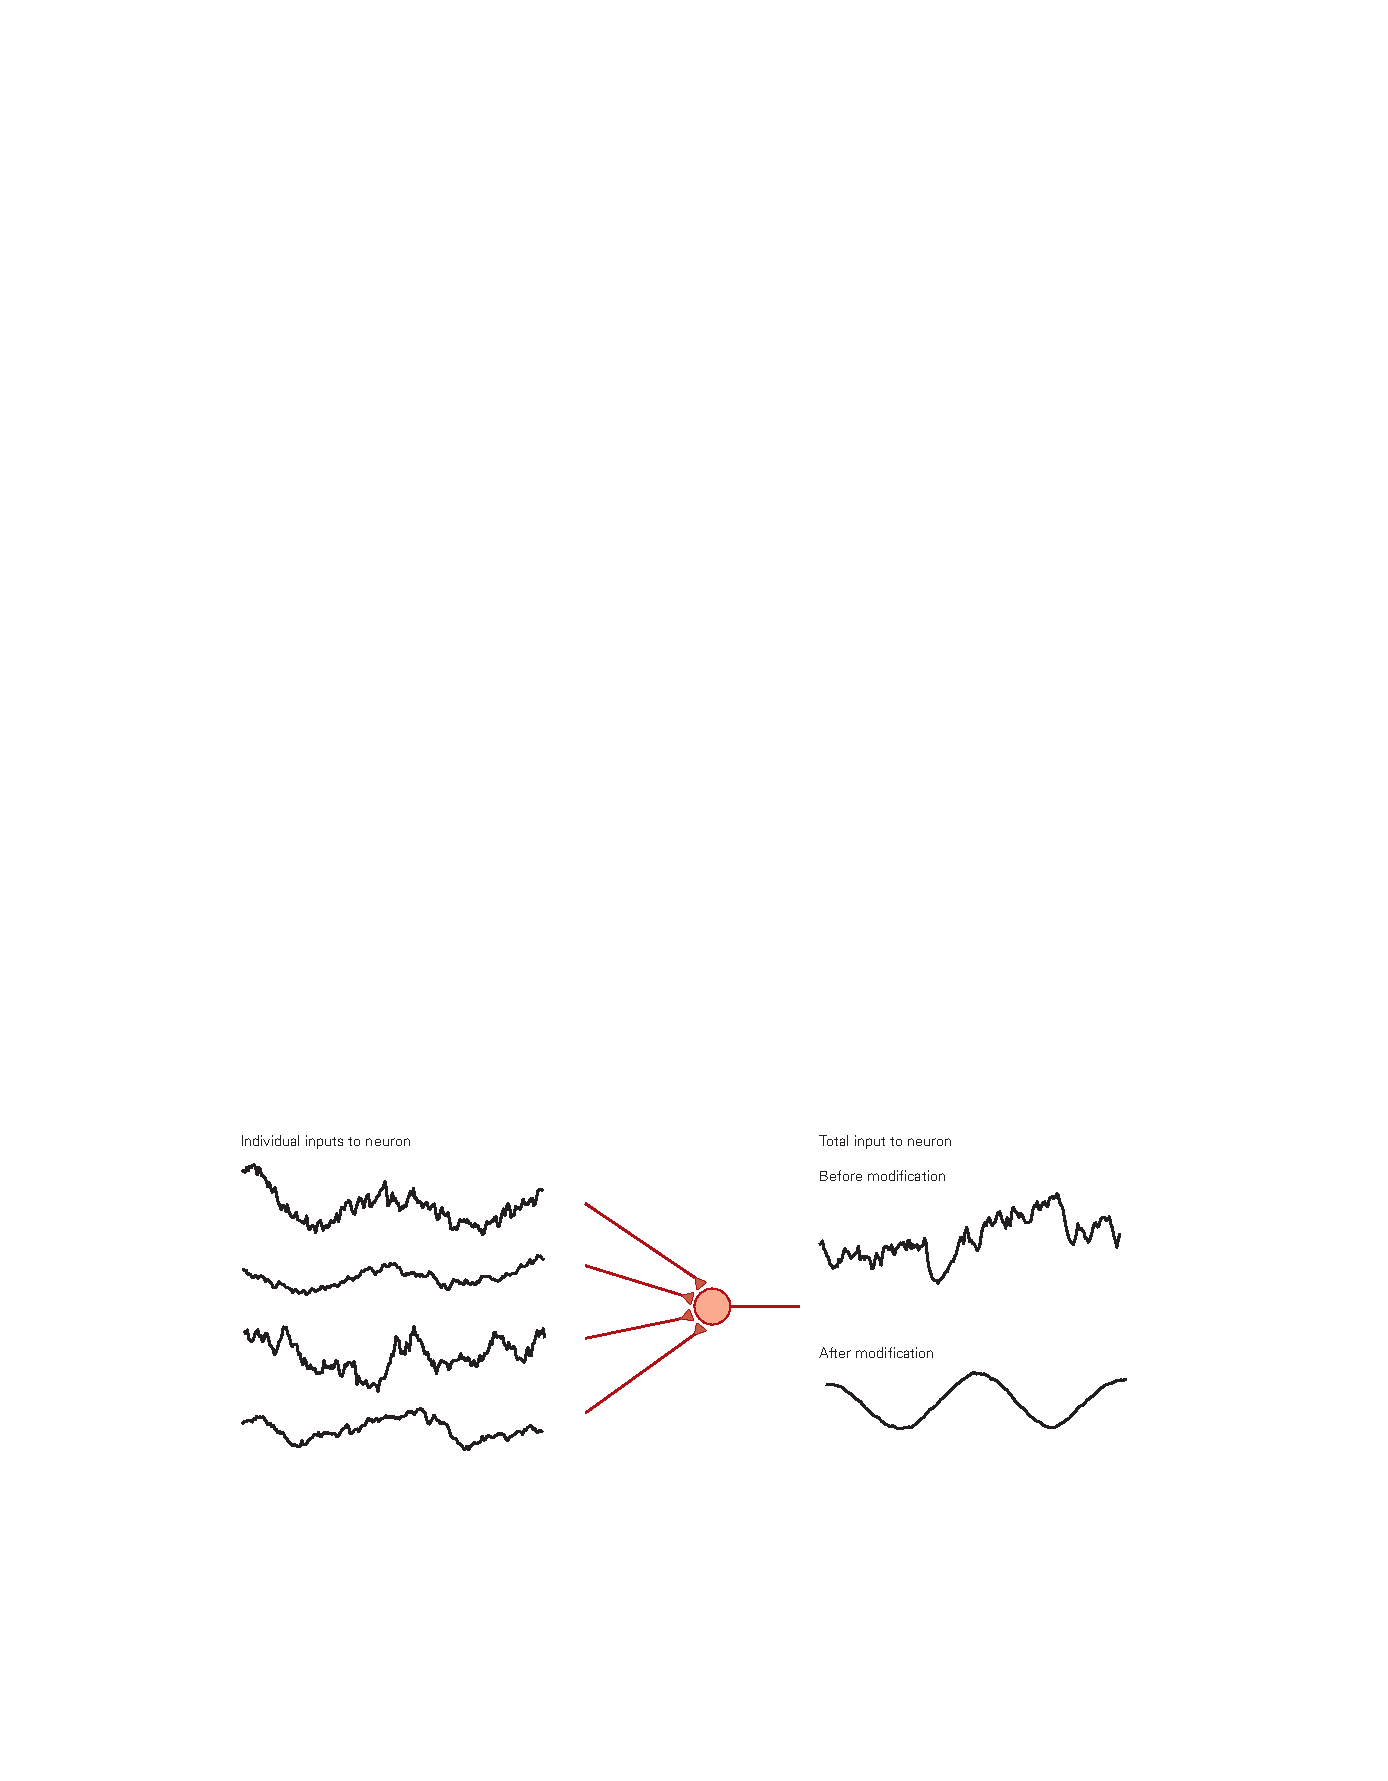
\includegraphics[width=1.0\linewidth]{chap05/fig_5_7}
	\caption{赫布可塑性可以识别神经元的相关输入信号。
		在这个例子中,一个神经元接收 100 个输入;
		显示了其中四个的激活率(左)。
		每个输入速率都有噪声,但在噪声中包含正弦信号。
		输入速率乘以突触强度(棕色三角形),然后求和以产生神经元的总输入(右)。
		在\textit{赫布可塑性}发生之前,突触具有随机权重,导致噪声轨迹;
		修改后,总输入揭示了潜在的正弦信号。}
	\label{fig:5_7}
\end{figure}


\subsection{小脑的突触可塑性在运动学习中起着关键作用}

尽管缺乏对小脑如何促进复杂人类运动技能的详细了解,但人们对其在简单形式的运动学习中的作用了解很多。
其中研究最透彻的是一种被称为\textit{延迟性眨眼条件反射}的范例,其中中性感官刺激(例如光或音调)与厌恶的\textit{非条件刺激}(例如向眼睛吹气)反复配对。
经过几天的此类训练,动物学会闭上眼睛以响应先前的中性刺激(光线或音调),称为\textit{条件刺激},以期待\textit{非条件刺激}(吹气)。
眼睑闭合的时间对于\textit{条件刺激}发作和\textit{非条件刺激}之间的延迟具有高度特异性。


眼睑条件反射一直是理解小脑功能的一个非常有用的范例,因为它以一种特别清晰的方式映射到小脑回路的结构上(图~\ref{fig:5_8})。
有关\textit{条件刺激}的信息首先由小脑颗粒细胞编码,然后传递给浦肯野细胞。
\textit{非条件刺激}由一个完全独立的输入通路编码,称为橄榄小脑或攀爬纤维系统。
与来自颗粒细胞的数千个输入相反,每个浦肯野细胞从称为下橄榄的脑干核接收单个强大的攀爬纤维输入。
电生理记录显示,向小脑某一特定区域输入的攀爬纤维表示\textit{非条件刺激}的发生,即刺激角膜的刺激。
这一发现之所以成为可能,是因为攀爬纤维在浦肯野细胞中引起了一种独特的超阈值反应,称为复杂尖峰。


\begin{figure}[htbp]
	\centering
	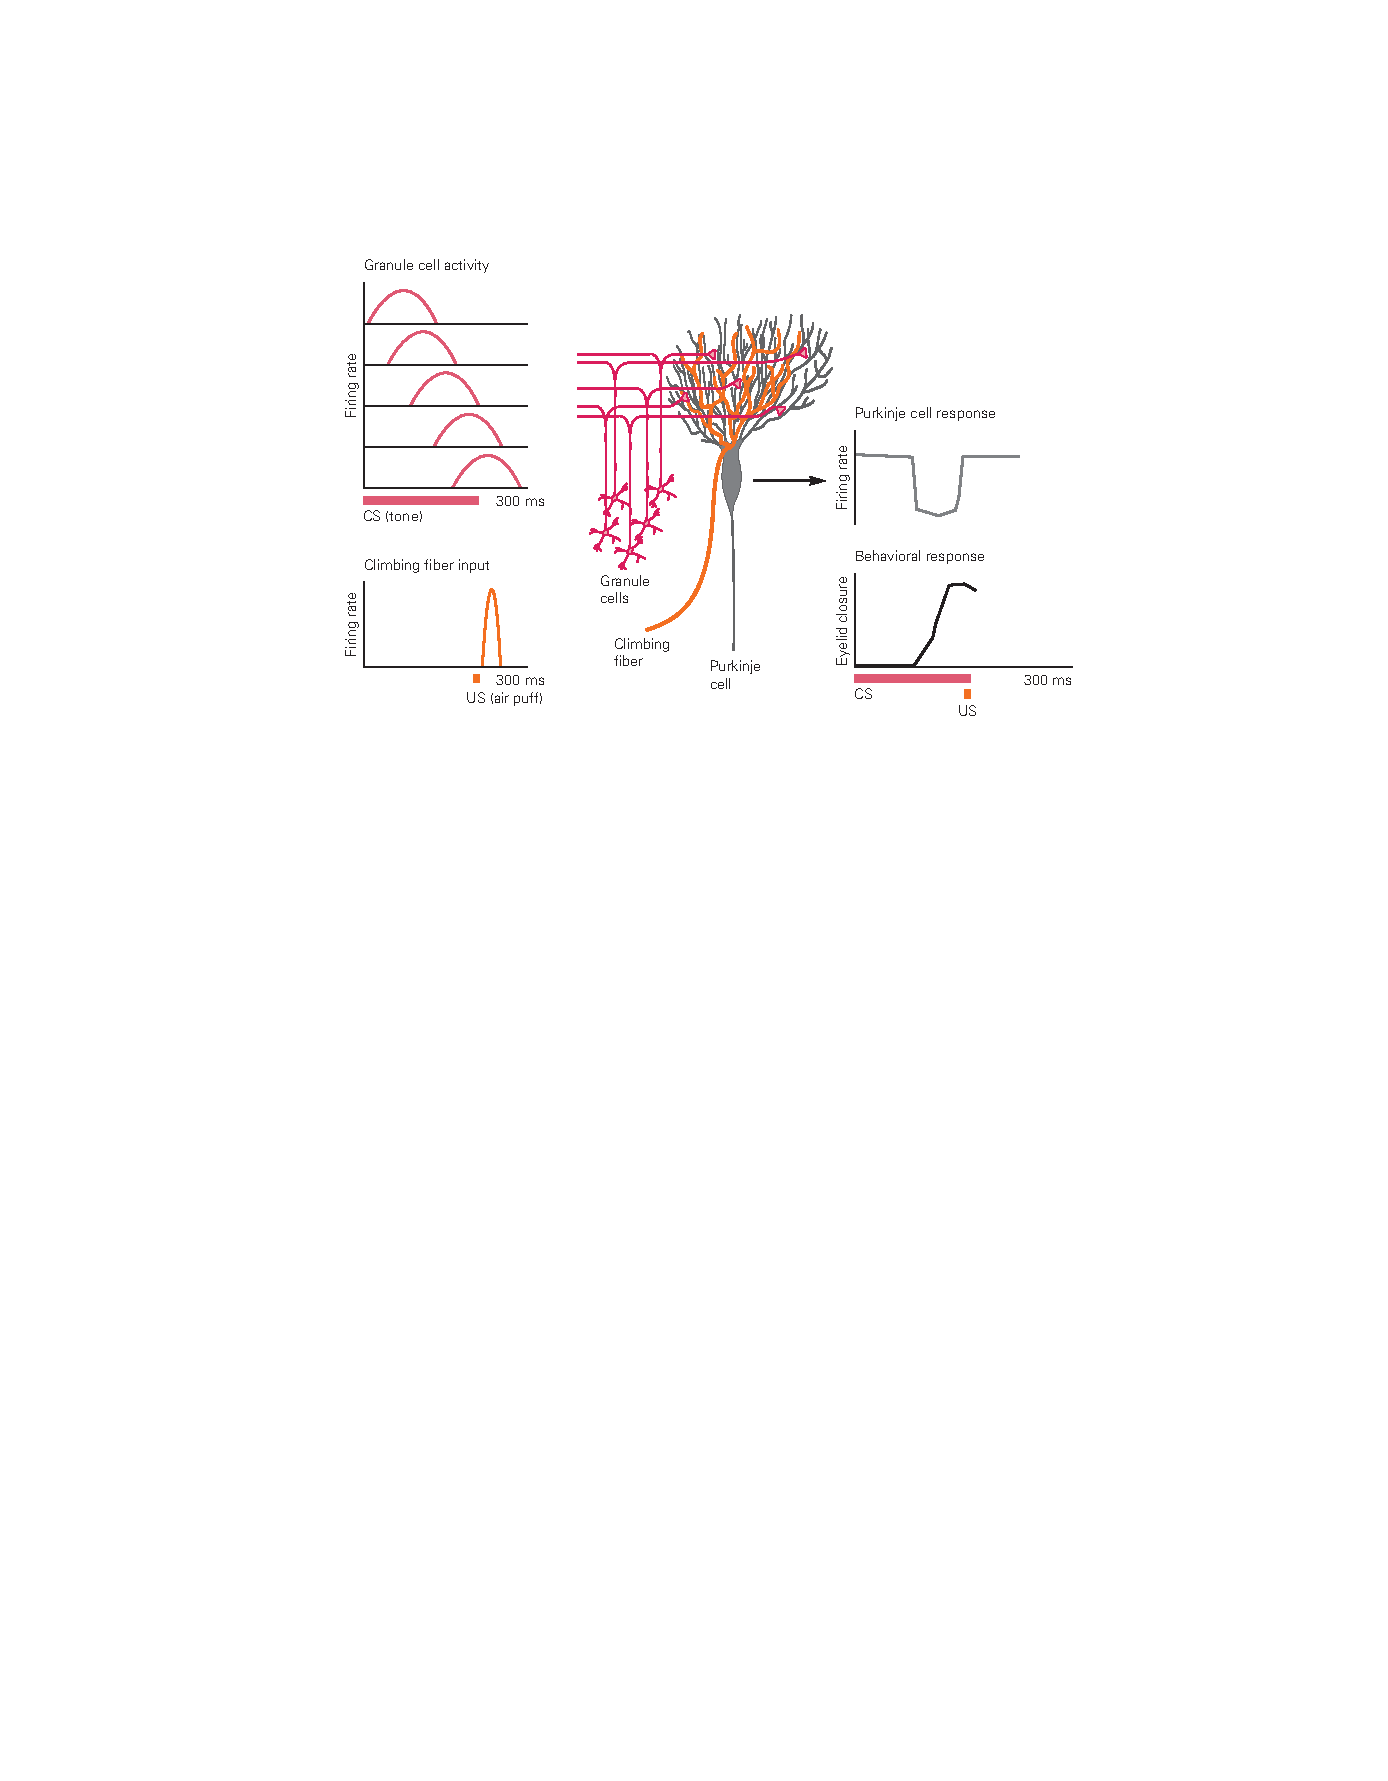
\includegraphics[width=0.92\linewidth]{chap05/fig_5_8}
	\caption{小脑在眨眼条件反射中的假设作用。
		有关\textit{条件刺激}和\textit{非条件刺激}的信息分别通过苔藓和攀爬纤维通路传递。
		在\textit{非条件刺激}呈现之前活跃的颗粒细胞突触被攀爬纤维输入引起的长期抑制逐渐减弱。
		这有助于浦肯野细胞激活的暂停,恰好在\textit{非条件刺激}之前发生。
		由于浦肯野细胞是抑制性的,这种暂停会激发小脑核和红核中的下游神经元,从而驱动眼睑闭合。}
	\label{fig:5_8}
\end{figure}


了解小脑如何调节学习的关键是发现复杂的尖峰触发颗粒细胞和浦肯野细胞之间突触的可塑性。
具体来说,来自突触前颗粒细胞的输入与突触后浦肯野细胞中的复杂尖峰同时出现,导致颗粒细胞输入持续减弱,这是一种称为小脑长期抑制的可塑性形式(图~\ref{fig:5_8})。
因此,对于\textit{非条件刺激}的每次出现,在\textit{非条件刺激}之前立即激活的颗粒-浦肯野细胞突触的强度都会降低。
由于在\textit{非条件刺激}预期到达时间之前颗粒细胞兴奋减少,这种可塑性导致浦肯野细胞放电中逐渐出现学习性暂停。


浦肯野细胞放电的减少如何导致习得性运动反应?
浦肯野细胞通常是自发活动的,它们会抑制下游靶点。 
小脑区域的浦肯野细胞接收与眼睛有害刺激相关的攀爬纤维输入,与神经元形成突触,间接激活产生眼睑闭合的肌肉。
因此,习得的浦肯野细胞放电暂停导致眼睑在正确的时刻闭合以保护眼睛。
适当的暂停时间被认为是由颗粒细胞的时间反应模式的多样性介导的。
计算机仿真表明,如果单个颗粒细胞在\textit{条件刺激}后的不同延迟处活跃或表现出锁定到\textit{条件刺激}的各种不同但可重复的时间模式,则可以通过颗粒-浦肯野细胞突触的可塑性来解释适当定时响应的学习。


由于技术挑战,对于参与眨眼调节的哺乳动物小脑区域的颗粒细胞,尚未获得此类时间表征的直接证据。
然而,在类似于鱼类小脑的结构中的颗粒细胞中观察到了多种时间模式。
更广泛地说,对小脑的研究,包括对眨眼条件反射的研究,提供了一个具体的例子,说明神经回路如何通过反复试验来调节学习,甚至是学习更复杂的运动技能,如演奏乐器。
浦肯野细胞整合了与动物的外部世界和内部状态相关的丰富多样的信号(由颗粒细胞传递),以及关于错误或意外事件的高度特异性信息(由攀爬纤维传递)。
攀爬纤维起到老师的作用,削弱了之前活跃的突触,因此可能导致错误。
突触强度的这些变化改变了浦肯野细胞的放电模式,并凭借特定的布线模式改变了行为,从而逐渐减少了错误。


小脑和大脑皮层,包括海马区,是关于学习和记忆的大量实验和理论研究的焦点。 
技术进步为研究突触动作、单个细胞和电路对记忆相关现象的贡献开辟了新的途径。



\section{亮点}

1. 神经编码描述了神经元活动如何表示刺激的特征或预期的行为。
解码是指解释神经活动来揭示编码信号的逆过程。
神经反应的数学解码可用于解释神经回路执行的计算并驱动假肢装置。 


2. 神经回路高度相互关联,但使用了一些基本主题来表征它们的功能和操作模式。 
前馈回路处理信息以从感觉流中提取结构和意义。 
循环回路可以执行时间处理并生成动态活动以驱动运动响应。


3. 大多数神经元接受兴奋性和抑制性输入的微调平衡。 
这种平衡响应感官刺激的微小变化可以唤起动作电位输出。


4. 神经活动的水平通常必须维持数秒。 
循环激发网络提供了一种机制来产生神经输出的持久变化。


5. 突触可塑性支持构成学习和记忆基础的神经回路的更持久变化。
赫布可塑性可以从一组复杂的输入中提取有趣的信号,而无需监督(“老师”)。
小脑皮层的突触可塑性由\textit{误差信号}(一种监督形式)驱动,并用于调整运动反应和学习时间关系。




\chapter{成像和行为} \label{chap:chap6}

为了用生物学术语解释生物体的行为,有必要协调生物学过程的测量(例如,动作电位、血流、神经递质的释放)与认知和运动输出的测量。
然而,将生物和行为措施联系起来具有挑战性。
对非人类动物进行精确的神经测量和侵入性技术是可能的,但其中许多物种的行为库相对有限。
此外,直接测量或侵入性地操纵健康人类的神经活动要困难得多,健康人类是具有最先进和最多样化行为的物种。
因此,现代神经科学的核心努力一直是开发新方法,以从人脑中获取精确的生物学测量值,并在非人类动物中模拟人类行为。


人类测量生物过程并将其与行为联系起来的主要方法是\textit{功能性核磁共振成像}。
\textit{脑电图}、\textit{正电子发射断层扫描}和\textit{近红外光谱}等其他测量人脑功能的成像方法各有长处。
然而,由于多种原因,功能性核磁共振成像特别适合研究人类行为的神经基础。
首先,它是非侵入性的:它不需要手术、电离辐射或其他破坏性干预。
其次,它可以在短时间内(以秒为单位)测量大脑功能,这使其能够捕捉心理过程和行为的动态方面。
第三,它同时测量整个大脑的活动,提供了检查多个大脑区域如何相互作用以调节复杂行为的机会。
因此,本章的重点是功能性核磁共振成像。


我们首先解释功能性核磁共振成像实验如何工作的技术细节以及通常如何收集数据。 
然后我们解释如何分析功能性核磁共振成像数据以及它们如何提供对人类行为和思想的洞察力。 
然后,我们将使用来自感知、记忆和决策领域的示例,对从功能性核磁共振成像中学到的内容进行更概念性的概述。
最后,我们考虑功能性核磁共振成像的优势和局限性,并讨论它可以支持的关于大脑和行为的推断类型。


虽然本章的重点是健康大脑的成像和行为,但功能性核磁共振成像也有可能改变我们诊断和治疗精神和神经疾病的方式。
几乎所有此类疾病(例如,孤独症、精神分裂症、抑郁症、\textit{进食障碍})除了特定大脑区域和细胞类型的破坏之外,还涉及大规模回路动力学的变化。
对健康大脑回路如何调节心理过程和行为的基础研究,结合在临床人群中测量这些相同回路活动的能力,为理解疾病和功能失调行为带来了巨大希望。



\section{功能性核磁共振成像实验测量神经血管活动}

功能性核磁共振成像实验使研究人员能够根据响应神经活动而发生的局部血氧水平变化来追踪大脑功能。
与所有形式的核磁共振成像一样,功能性核磁共振成像需要高度专业化的设备和复杂的计算机程序。
在本节中,我们首先考虑如何使用核磁共振成像对大脑\textit{结构}成像的基本原理,然后解释功能性核磁共振成像如何将此功能扩展到对大脑\textit{活动}成像。


每台核磁共振成像机器的核心都是强大的磁铁。
磁场强度以\textit{特斯拉}为单位进行量化,大多数现代\textit{核磁共振成像}机器都是 3 \textit{特斯拉}。
使用像 7 \textit{特斯拉}这样更高的场强会提供了一些优势,包括对皮层进行更高分辨率成像的可能性。
此类机器还没有普及,层特定成像还处于起步阶段,所以我们关注 3 \textit{特斯拉}机器的能力和配置。


% % The outside of an MRI machine looks like a tunnel, known as the “bore” of the magnet. 
核磁共振成像仪的外部看起来像一条隧道,被称为磁铁的“孔”。
% Subjects lie on a bed with their head in a helmet-like head coil, which receives signals from the brain. 
受试者躺在床上,头戴头盔状的头部线圈,接收来自大脑的信号。
% Visual stimuli are typically viewed through a mirror on the head coil angled toward a screen at the back of the bore.
视觉刺激通常通过头部线圈上的镜子观察,镜子与孔后部的屏幕成一定角度。
% Auditory stimuli are presented through headphones. 
听觉刺激通过耳机呈现。
% Behavior is typically measured in terms of manual responses with a button box and/or eye movements with an eye tracker.
行为通常根据使用按钮框的手动响应和/或使用眼动仪的眼球运动来衡量。
% This apparatus constrains which experimental tasks are possible. 
该设备限制了哪些实验任务是可能的。
% However, fMRI is flexible in other ways, including that it can be performed and repeated without harm in many different types of subjects, from children to the elderly, whether healthy or suffering from a disorder.
然而,功能性核磁共振成像在其他方面也很灵活,包括它可以在许多不同类型的受试者身上进行和重复,而不会造成伤害,从儿童到老人,无论是健康的还是患有疾病的。


% What does fMRI measure? 
功能性核磁共振成像测量什么?
% There are two fundamental concepts that we will discuss in turn, first magnetic resonance and then neurovascular coupling (Figure 6–1).
我们将依次讨论两个基本概念,首先是\textit{磁共振},然后是\textit{神经血管耦合}(图~\ref{fig:6_1})。


\begin{figure}[htbp]
	\centering
	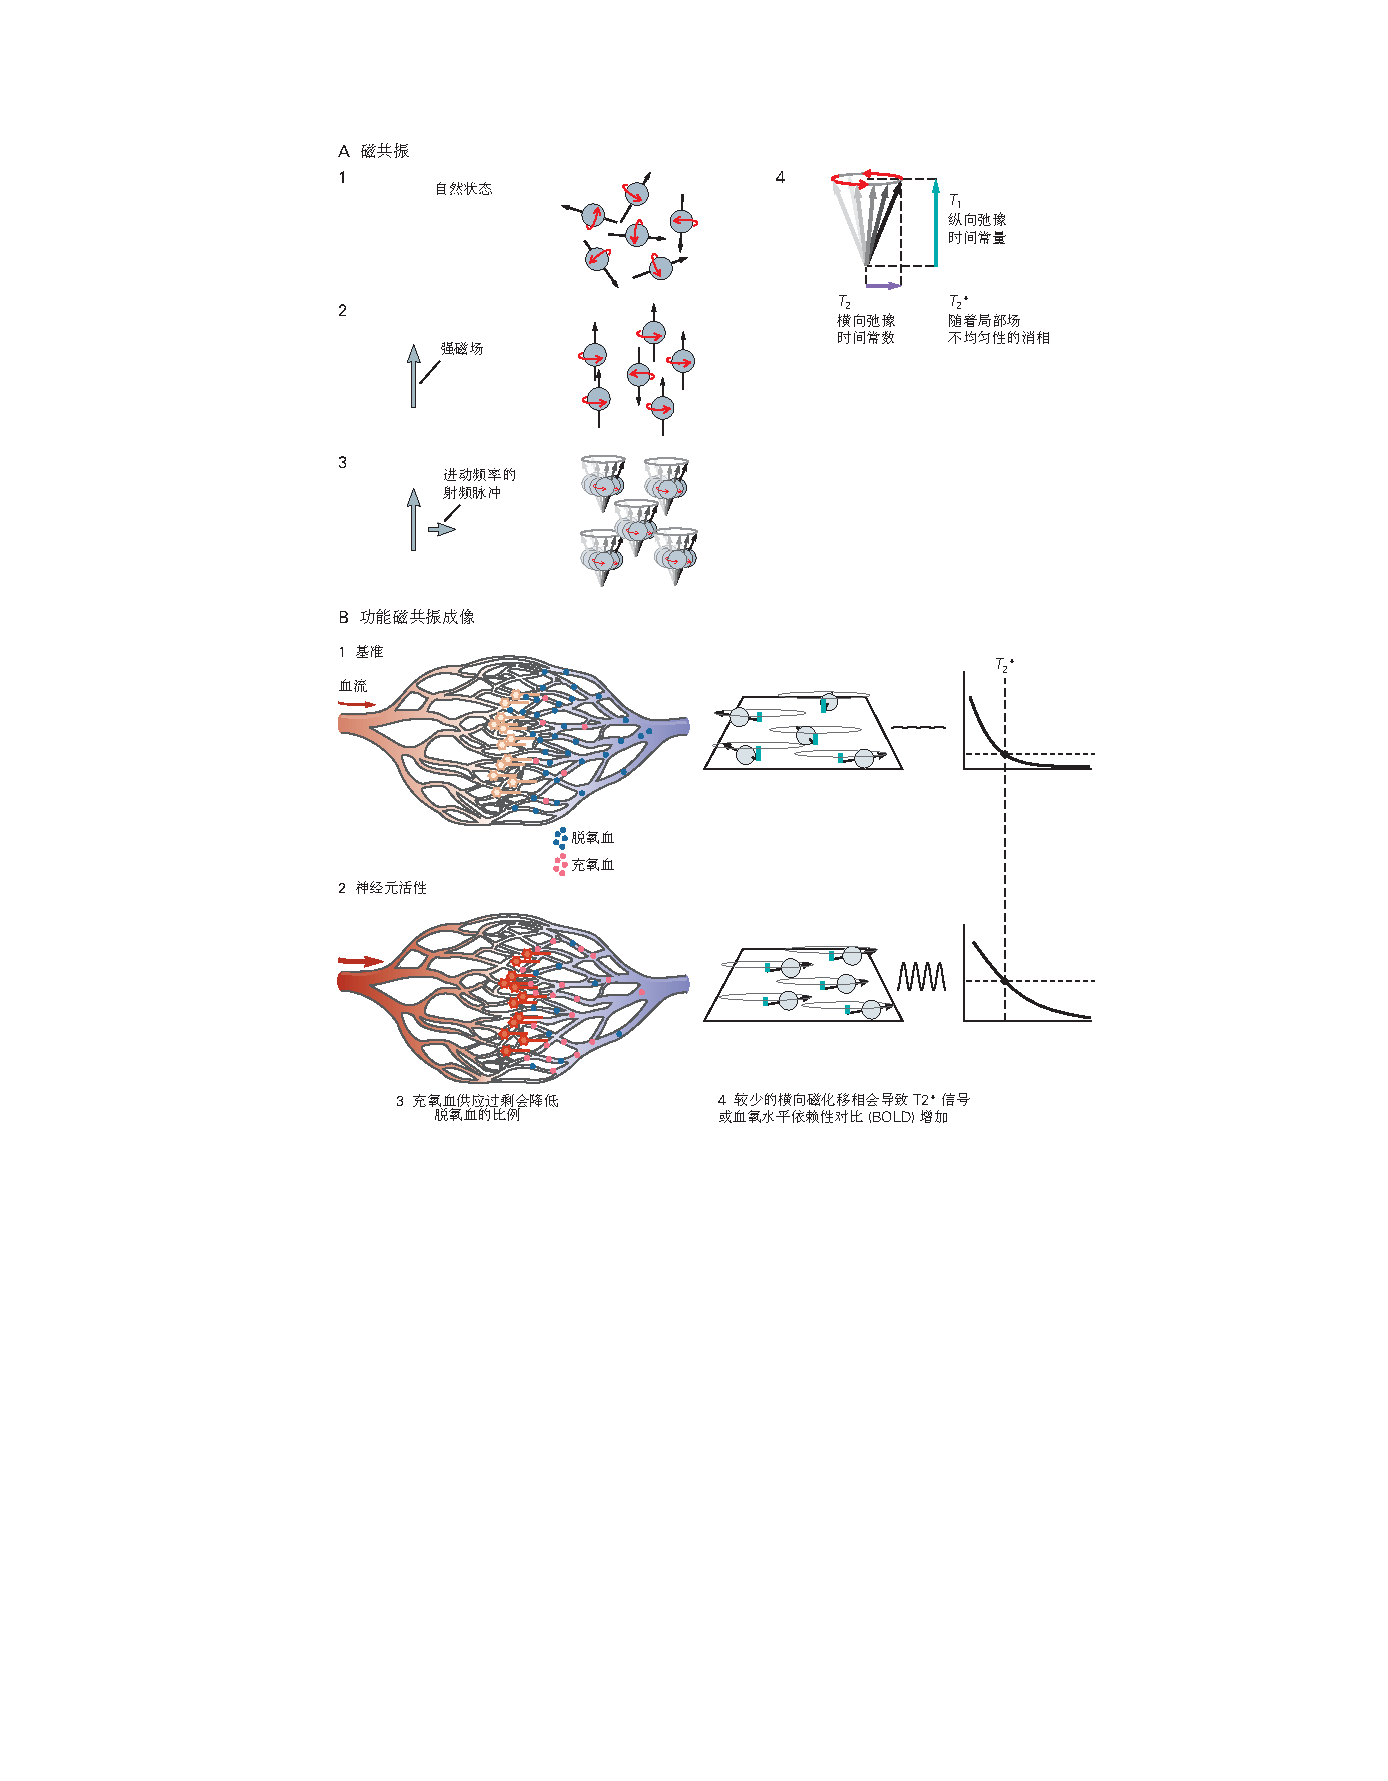
\includegraphics[width=0.9\linewidth]{chap06/fig_6_1}
	\caption{\textit{功能性核磁共振成像}如何测量神经活动。
		\textbf{A.} 在核磁共振环境之外,大脑中氢原子中的质子围绕指向随机方向的轴旋转(1)。
		当大脑进入核磁共振成像孔的强磁场时,这些轴的子集与该磁场对齐,这被称为纵向磁化(2)。
		这些质子可以通过发射射频脉冲来测量,射频脉冲会感应出垂直于强磁场的较弱磁场。
		这会使质子与强场错位,强场现在充当扭矩,导致质子自旋轴在横向平面上以弧形进动。
		选择射频脉冲的频率以与质子的进动速率共振,而质子的进动速率又取决于磁场强度(3)。
		当射频脉冲停止时,质子最初继续同步进动,在头部周围的接收线圈中感应出相同频率的交流电。
		这些信号可用于通过应用磁梯度来生成图像,磁梯度可调整整个大脑正交方向的场强。
		这会在大脑的不同点产生不同的共振频率,从而可以识别接收信号的来源。
		横向磁化随时间消散,信号丢失。
		这种弛豫发生在质子释放热力学能量并且它们的轴返回纵向方向(T1)时,并且由于质子在横向平面中由于与其他原子和分子的局部相互作用而变得不同步(T2),并且由于质子中的不均匀性 磁场(T2 *)(4)。
		\textbf{B.} 由于血液的磁性,磁共振可用于估计功能性核磁共振成像中的神经元活动。
		% 活跃时需要更多的血
		当大脑区域处于基线状态时,脱氧血与充氧血的比例高于该区域活跃时的比例。
		% 脱氧血红蛋白(即没有携带氧的血红蛋白)中的每个铁原子都有4个未配对的电子,使得脱氧血红蛋白具有微弱的顺磁性;
		% 但氧合血红蛋白(即携带了氧气的血红蛋白)中的铁原子没有未配对电子,使得氧合血红蛋白具有抗磁性。
		脱氧血与磁场相互作用,导致局部不均匀性,从而扭曲进动速率并破坏横向平面中质子的同步,导致更快的 T2 * 衰减和更低的\textit{血氧水平依赖}信号(1)。
		神经元活动导致代谢需求(2),进而导致输送过量的氧合血(3)。
		含氧血液不与磁场相互作用,因此活跃大脑区域的含氧量增加会减少场的不均匀性。
		反过来,这减少了质子在横向平面进动的相位差,导致更慢的 T2 * 衰减和更高的\textit{血氧水平依赖}信号(4)。}
	\label{fig:6_1}
\end{figure}



% fMRI Depends on the Physics of Magnetic Resonance
\subsection{功能性核磁共振成像取决于磁共振物理学}

% In general, MRI exploits the magnetic properties of hydrogen atoms, the dominant source of protons in the body, specifically the way each atom’s proton interacts with a strong magnetic field. 
一般来说,核磁共振成像利用氢原子的磁性,氢原子是体内质子的主要来源,特别是每个原子的质子与强磁场相互作用的方式。
% A key property of protons is that they intrinsically rotate around an axis. 
质子的一个关键特性是它们本质上围绕一个轴旋转。
% This spin gives protons angular momentum and a magnetic dipole along the axis, their own north and south poles. 
这种自旋给质子提供了角动量和沿它们自己南北极轴的\textit{磁偶极子}。
% Under normal circumstances, the directions of these dipoles are random for different protons.
在正常情况下,这些偶极子的方向对于不同的质子是随机的。
% When placed in a strong external magnetic field, however, a subset of the protons (how many is proportional to the field strength) align with the direction of this field, which extends from foot to head when lying in an MRI bore.
然而,当置于强外部磁场中时,质子的子集(数量与场强成正比)与磁场方向对齐,当位于核磁共振成像孔中时,质子从脚延伸到头部。


% In the case of a 3T magnet and hydrogen atoms, this speed is in the radiofrequency (RF) range.

% An important step toward measuring a signal from protons is to push them out of alignment with this main field. 
测量质子信号的一个重要步骤是将它们推离这个主场。
% To understand why, it is helpful to think about a familiar object, the gyroscope. 
要理解其中的原因,不妨想想一个熟悉的物体,即陀螺仪。
% If a still gyroscope is tipped out of vertical balance, it will just fall over. 
如果一个静止的陀螺仪失去垂直平衡,它就会翻倒。
% However, if you spin the gyroscope before tipping it, inertial forces will prevent it from falling over. 
但是,如果在倾斜陀螺仪之前先旋转它,惯性力会防止它翻倒。
% The axis around which the gyroscope is spinning will itself begin to rotate around the vertical axis. 
围绕自身轴旋转的陀螺仪将开始围绕垂直轴旋转。
% This precession occurs because gravity exerts a vertical torque on the tilted gyroscope, pulling its center of mass down so that it pivots around its bottom point and traces out a circle in the transverse plane (looking from above).
发生这种进动是因为重力对倾斜的陀螺仪施加垂直扭矩,将其质心拉下,使其围绕其底部点旋转并在横向平面(从上方看)中划出一个圆圈。 
% Something similar happens to a proton that is tilted with respect to the strong magnetic field: The field applies a torque and the orientation of the rotational axis precesses around the field direction. 
相对于强磁场倾斜的质子也会发生类似的情况:磁场施加扭矩,旋转轴的方向围绕磁场方向进动。
% The speed of precession, or the resonant frequency, is determined by the Larmor equation, according to the field strength and a gyromagnetic ratio specific to each type of atom. 
进动速度或共振频率由\textit{拉莫尔方程}根据场强和每种原子特有的旋磁比确定。 
对于 3 \textit{特斯拉}磁体和氢原子,该速度处于\textit{射频}范围内。



% But how do protons get tipped out of alignment in the first place to enable precession?
但是,质子是如何从一开始就偏离排列以实现进动的呢? 
% The answer depends upon the same principle of torque. 
答案取决于扭矩的相同原理。 
% A second, weaker magnetic field is applied in a perpendicular direction (eg, front to back of the head), introducing another torque that pulls protons away from alignment with the strong field. 
第二个较弱的磁场在垂直方向(例如,从头部的前部到后部)施加,引入另一个扭矩,将质子拉离与强磁场对齐的位置。
% This misalignment causes precession about the direction of the strong field by allowing the strong field to act as a torque. 
这种未对准通过允许强场充当扭矩而导致围绕强场的方向的进动。
% Complicating matters, this precession makes protons a moving target for the weaker magnetic field that is needed to cause misalignment in the first place. 
使事情复杂化的是,这种进动使质子成为首先导致错位所需的较弱磁场的移动目标。
% This is solved by generating the second field using a transmit coil in the MRI machine, through which alternating current is passed to deliver an RF pulse at the resonant frequency of the protons. 
这是通过使用核磁共振仪中的发射线圈生成第二个场来解决的,交流电通过该线圈以在质子的共振频率下传递射频脉冲。
% This induces a perpendicular magnetic field that rotates in lockstep with the precession. 
这会产生一个垂直磁场,该磁场会随着进动同步旋转。
% This RF pulse is sustained as long as needed to generate a specified change in the spin orientation of protons away from the strong field direction (eg, 90°). 
该射频脉冲的持续时间与产生质子自旋方向远离强场方向(例如 90°)的指定变化所需的时间一样长。
% This change is known as the flip angle and is often chosen to maximize signal according to the Ernst equation.
这种变化被称为翻转角,通常根据 \textit{能斯特方程}选择它来最大化信号。


% Once the desired flip angle has been achieved, the RF pulse is stopped in order to measure the composition of tissue. 
一旦达到所需的翻转角,射频脉冲就会停止以测量组织的成分。
% At this point, protons are precessing around the strong magnetic field and tilted heavily into the transverse plane. 
此时,质子在强磁场周围进动并严重倾斜到横向平面中。
% This is akin to a bar magnet spinning on a table, where the north and south poles take turns passing any given location. 
这类似于在桌子上旋转的条形磁铁,北极和南极轮流经过任何给定位置。
% If a coil is placed nearby, the spinning magnet induces a current in the wire that reverses as the poles alternate. 
如果在附近放置一个线圈,旋转的磁铁会在电线中感应出电流,该电流会随着磁极交替而反转。
% This is what the receiver head coil in an MRI machine measures: alternating current induced by protons precessing synchronously (note: this is the same principle as described earlier for how the transmit coil works, just reversed). 
这就是核磁共振成像仪中的接收头线圈所测量的:由同步进动的质子感应的交流电(注意:这与前面描述的发射线圈的工作原理相同,只是相反)。
% The amount of current indicates the concentration of precessing protons.
电流量表示进动质子的浓度。


% Critically, the frequency of these measured signals reflects the speed of precession, which in turn depends on the strength of the magnetic field experienced by the tissue. 
至关重要的是,这些测量信号的频率反映了进动的速度,而进动的速度又取决于组织所经历的磁场强度。
% This can be used to generate three-dimensional images by imposing different gradients on the magnetic field (think of a staircase from higher to lower strength) that cause the Larmor frequency to vary systematically over space in the brain. 
这可用于通过在磁场上施加不同的梯度(想象从强度从高到低的阶梯)来生成三维图像,从而导致拉莫尔频率在大脑空间内系统地变化。
% During fMRI, one gradient is applied in a specific direction to select a slice of brain tissue. 
在功能性核磁共振成像期间,在特定方向上应用一个梯度以选择脑组织切片。
% The RF pulse can be tailored to the resonant frequency for the exact field strength at this gradient step, such that only protons in this slice are excited. 
可以针对此梯度步骤中的精确场强将射频脉冲调整为共振频率,以便仅激发该切片中的质子。
% The same logic is used with additional gradients in orthogonal directions to impose a two-dimensional matrix on the selected slice, with each unit volume in the matrix or voxel having a unique frequency and phase. 
相同的逻辑与正交方向上的附加梯度一起使用,以在所选切片上施加二维矩阵,矩阵或体素中的每个单位体积具有唯一的频率和相位。
% The head coil receives a composite signal with a mixture of these frequencies, but the signal can be decomposed to identify protons at every voxel in the slice.
头部线圈接收混合了这些频率的复合信号,但信号可以被分解以识别切片中每个体素处的质子。


进动质子还有另一个有助于核磁共振成像的重要特性:
在射频脉冲之后,头部线圈中感应的交流电开始衰减。
腐烂有不同的来源。
一个来源是进动质子向周围组织释放热力学能量(热量),就像陀螺仪最终会因摩擦而失去能量并翻倒。
当这种情况发生时,质子的自旋方向逐渐放松回到强磁场的方向,导致它们在横向平面内的进动减少,从而产生较少的信号。
这称为纵向弛豫并以时间常数 T1 发生。
第二种类型的衰变发生在质子仍在横向平面内进动时。
单个质子被其他原子的可变邻域包围,这些原子带有自己的弱磁场。
这会微妙地改变质子所经历的场强,导致其拉莫尔频率发生不可预测的变化。
而在\textit{射频}脉冲质子同步进动之后,这些局部相互作用会导致一些质子进动得更快或更慢。
由于它们越来越不同步,感应电流交替的可靠性降低,信号丢失。
这称为横向弛豫并以时间常数 T2 发生。 
质子的这种去相位也可能是强磁场本身的不均匀性造成的,包括它如何被置于磁场中的组织扭曲。 
来自局部相互作用和场失真的信号衰减具有时间常数 T2 *(发音为“T2-星”)。


这些不同的衰变源很重要,因为 T1 和 T2 时间常数因组织类型而异。 
因此,\textit{核磁共振成像}可以利用信号衰减来识别灰质、白质、脂肪和/或脑脊液。 
根据\textit{核磁共振成像}机器上设置的\textit{射频}脉冲、梯度和其他参数(统称为脉冲序列)的配置和时间,从不同体素接收的信号可以突出具有不同 T1 值的组织之间的对比度(T1 加权图像 ) 和/或不同的 T2 值(T2 加权图像)。 
例如,在 T1 加权图像中,白质比灰质更亮,而 T2 加权图像则相反。


测量脑功能的标准脉冲序列是\textit{平面回波成像}序列。 
\textit{平面回波成像}对\textit{功能性磁共振成像}有两个理想的特性:它非常快,允许在不到 100 毫秒的时间内从一个\textit{射频}脉冲获取整个切片,并且它对 T2 * 敏感,我们稍后将看到,这就是\textit{核磁共振成像}测量的方式 神经活动。 
在设计\textit{功能性磁共振成像}研究时,需要选择\textit{平面回波成像}序列的几个参数,包括在脑体积中获取多少切片(通常为 30-90); 
每卷多少时间(重复时间,通常为 1-2 秒); 使用何种体素分辨率(每个维度通常为 2-3 毫米); 
以及是否使用并行采集(例如,一次采集切片的多个部分和/或多个切片)。
这些选择是相互依存的,需要在速度、精度和信噪比之间进行权衡。



\subsection{功能性核磁共振成像依赖于神经血管耦合的生物学}

我们已经描述了磁共振的一般原理,但是故事的第二部分,神经血管耦合呢?
活跃的神经元消耗从血液中的氧气中获得的能量。 
因此,当大脑区域活跃时,血液中的氧合作用会在那一刻下降。
为了补充这些代谢资源,在接下来的几秒钟内流向局部的血液会增加。
供应超过需求,因此,与直觉相反,活跃的大脑区域中含氧(相对于脱氧)血液的比例更高。


要将此与磁共振联系起来,请记住 T2 * 衰变反映了由场不均匀性引起的质子相移。 
血液具有不同的磁性,具体取决于氧合作用:脱氧血液与磁场相互作用,因为血红蛋白中的铁是未结合的,而铁与氧结合的含氧血液则不会。
因此,脱氧血液会导致更快的 T2 * 衰减,并降低相对于含氧血液的信号。
这种信号差异称为血氧水平依赖性对比度。 
综上所述,用\textit{平面回波成像}序列测量的体素信号增加表明最近的神经元活动,因为伴随这种活动的局部血液氧合相对增加。
这种血氧水平依赖反应的时间曲线,称为血液动力学反应函数,看起来像一条长尾巴的钟形曲线,在局部神经活动后约 4 到 5 秒达到峰值,并在 12 到 15 秒后返回基线。
关于功能性核磁共振成像的物理学和生物学还有更多细节。 
此外,我们对这一切如何运作的理解仍在不断发展。 
例如,目前尚不清楚血氧水平依赖是否与单个神经元的放电或神经群体的活动更密切相关。 
同样,可能难以区分血液氧合作用增加是由局部兴奋或抑制增加引起的。 
更一般地说,神经血管耦合的机制(大脑如何知道何时何地输送含氧血液)仍然是个谜,人们越来越关注星形胶质细胞的功能作用。 
通过测量神经元活动精确部位的初始耗氧量(“初始下降”),也有可能获得更好的时间和空间分辨率,反映在脱氧血液中立即和局部上升,而不是延迟和更多弥漫性供氧过剩的血液。 
然而,即使理解不完全,功能性核磁共振成像也可以作为一种工具来定位由心理操作引起的人脑神经活动的变化。



\section{可以通过多种方式分析功能性核磁共振成像数据}

在进行功能性核磁共振成像实验时,研究人员将前面描述的神经血管测量与编程到人类受试者执行的计算机脚本中的认知任务联系起来。
该脚本通常会生成一系列运行,这些运行对应于连续的数据收集周期(即,连续的几个功能性核磁共振成像体积),通常持续 5 到 10 分钟。 
在每次运行中,通常通过显示视觉刺激或播放听觉刺激来向受试者展示几个试验。 
根据任务的不同,受试者可能会,例如,被动地查看或聆听刺激,对其做出决定,或将其存储在记忆中。 
按钮按下或眼球运动反应通常被收集为该试验中认知处理的行为指标。 
这些试验通常来自两个或多个任务条件,这些条件决定了刺激类型、任务难度或其他实验参数。 
在基本的减法设计中,试验分为实验条件和控制条件,它们是相同的,但有一个关键差异,其神经基础正在研究中。 
试验通常持续 2 到 10 秒,通常由几秒的可变或“抖动”间隔分隔。 
总之,此类会议通常持续长达 2 小时。


每个功能性核磁共振成像会话都会产生大量原始数据,在大脑中数十万个位置对血氧水平依赖响应进行数千次采样。 
这些数据如何转化为关于认知和行为的见解? 
许多功能性核磁共振成像分析方法都是可能的(方框~\ref{box:6_1}),但在大多数情况下,它们分为三类(图~\ref{fig:6_2})。 
我们首先描述所有三种类型共有的预处理步骤,然后解释每个步骤是如何进行的以及它能告诉我们什么。


\begin{proposition}[神经解剖学导航术语] \label{box:6_1}
	
	\quad \quad 与许多科学领域相比,大脑成像的基本方法具有显著的标准化。
	造成这种情况的一个主要原因是,自20世纪90年代中期\textit{功能性核磁共振成像}问世以来,广泛采用的软件包就已经问世。
	这些软件包是由研究小组创建和发布的,在流行之前,大多数都是开源的。
	
	\quad \quad 起初,它们包括用于预处理、对齐、分析模型和统计校正的工具。
	此后,他们引入了研究人员开发的新工具,包括非线性对齐、场图校正、非参数统计和并行化。
	
	\quad \quad 因此,几乎所有的\textit{功能性核磁共振成像}研究人员都使用一个或多个这样的包,至少在他们的分析管道中是这样。
	用于\textit{功能性核磁共振成像}分析的流行免费软件包包括:\href{https://afni.nimh.nih.gov}{AFNI}、\href{https://fsl.fmrib.ox.ac.uk}{FSL}、\href{https://www.fil.ion.ucl.ac.uk/spm}{SPM}。
	
	\quad \quad 除了这些专门的软件包,功能磁共振成像越来越多地被从数据科学的更普遍的角度来看待。
	这有两个原因。
	首先,功能磁共振成像产生了大量的数据,既包括在每次治疗中,也包括在已经进行的数千项研究中汇总的数据。
	因此,理解功能磁共振成像数据可以被认为是一个大数据问题。
	其次,数据非常复杂和嘈杂,感兴趣的认知信号很弱,很难找到。
	这带来了一个数据挖掘挑战,激励了许多计算机科学家。
	
	\quad \quad 这一趋势最具体的表现是\textit{功能性核磁共振成像}分析中机器学习的兴起。
	与数据科学的其他接触点包括与流数据的实时分析相关的挑战、网络分析和图论方法的应用、高性能计算集群和云系统的使用,以及研究人员公开共享数据的日益增长的实践(例如,\href{https://openneuro.org}{openneuro})、代码(在\href{https://github.com/}{GitHub}等服务上)和教育材料(例如,\href{https://brainiak.org/tutorials}{BrainIAK})。
	因此,脑成像领域将继续受益于计算机科学、工程、应用数学和统计学的进步。
	
\end{proposition}


\begin{figure}[htbp]
	\centering
	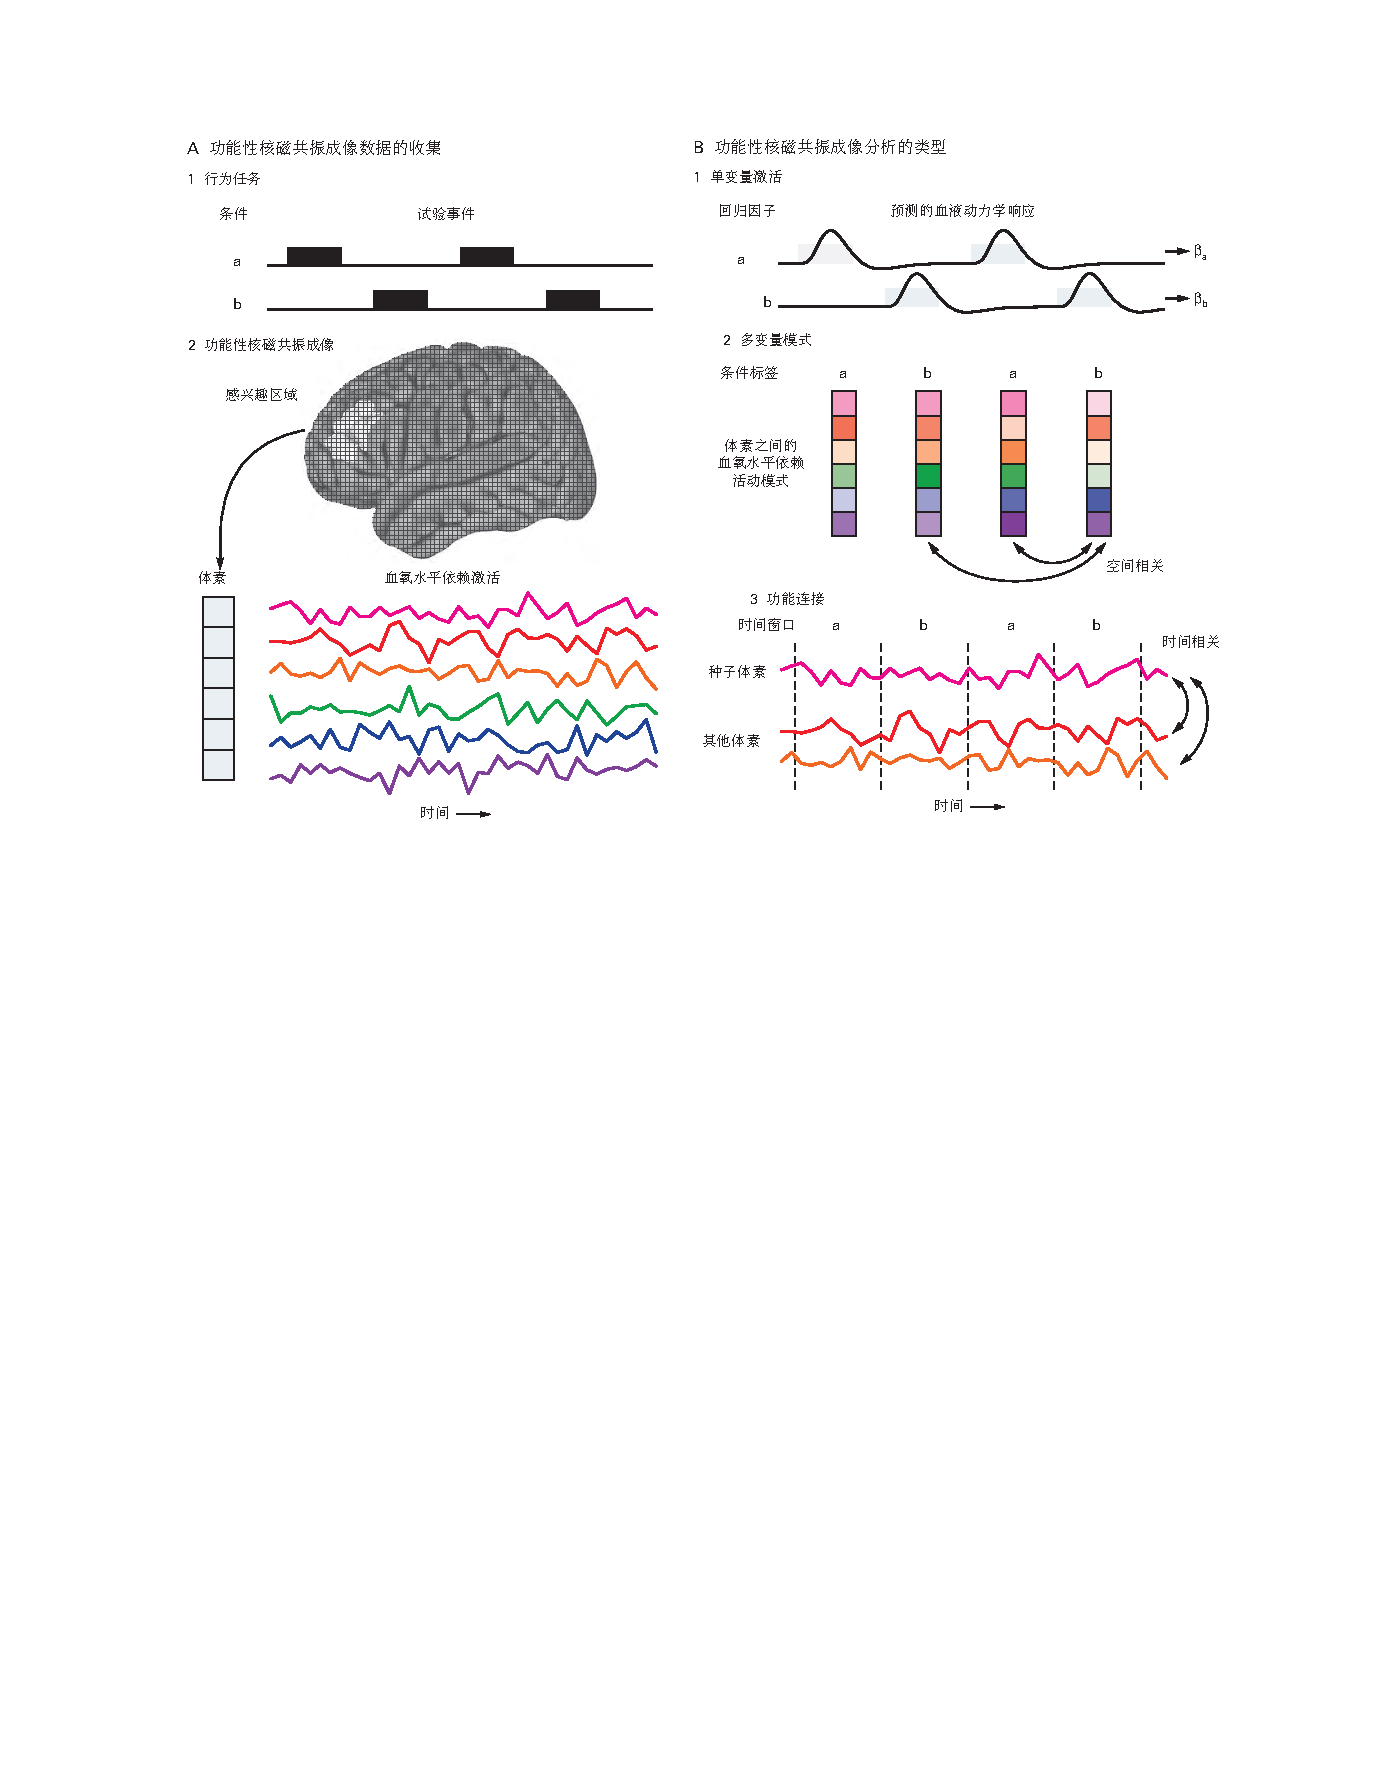
\includegraphics[width=1.0\linewidth]{chap06/fig_6_2}
	\caption{收集和分析\textit{功能性磁共振成像}数据。 
		\textbf{A.} 功能性核磁共振成像实验通常涉及受试者执行行为任务,同时从大脑测量血氧水平依赖活动。
		1. 示例任务包含两个在时间上交替出现的条件(a, b),每个条件都描绘了两个事件(黑色矩形)。
		2. 在任务期间,来自感兴趣区域的六个示例体素(不同颜色)中\textit{血氧水平依赖}活动的时间进程。 
		分析通常侧重于大脑中的感兴趣区域或其他体素子集,以减少执行的统计测试的数量。
		当分析大脑中的所有体素时,应用统计校正来减少误报的数量。
		此类分析的结果通常作为颜色编码的热图叠加在结构\textit{核磁共振成像}上。
		该图是广泛预处理和分析的结果,并不直接反映神经元活动甚至血液氧合。
		相反,体素是彩色的,以表明它们已经超过了在统计测试中被认为是重要的阈值。
		\textbf{B.} 功能性核磁共振成像实验中经常使用三种分析方法,例如 A 中描述的方法。
		1. 单变量激活分析试图根据任务中发生的情况来解释每个体素的血氧水平依赖活动。 
		这是使用统计模型完成的,该模型包含每个任务条件的回归变量,指定从该条件(灰色矩形)开始的试验事件的预测血液动力学响应(钟形曲线)。 
		将模型拟合到血氧水平依赖活动的结果是每个体素中每个回归量的$\beta$值,量化体素对该条件试验的平均响应。 
		可以减去体素的$\beta$值以衡量在一种情况下是否比另一种情况下有更大的响应。
		为了确定统计显着性,比较了受试者之间每个体素中条件之间激活的差异。
		2. 多变量模式分析考虑了跨体素的血氧水平依赖活动模式。
		这些空间模式是为每个试验从体素的一个子集(描绘了六个)中提取的,并且在特定时刻,通常是预测的血液动力学响应的峰值(颜色饱和度表示该试验中每个体素中 血氧水平依赖活动的幅度)。
		有两种常见的分析这些模式的方法。
		第一个(如图所示)涉及计算来自一对试验的模式的空间相关性,以探索体素对试验的反应有何相似之处。
		如果一个大脑区域代表不同条件下的不同信息,那么对于来自相同条件和不同条件的成对试验,这种模式相似性应该更高。
		第二种类型的多元模式分析(未显示)使用一种称为模式分类的机器学习。
		一些模式及其相应的条件标签用于训练分类器模型,根据它们在区分条件时的有用程度为体素分配权重。
		然后使用未训练的其他模式对该模型进行测试。
		如果大脑区域代表不同条件下的不同信息,则模型应该能够正确猜测从哪种条件下提取模式。
		为了确定统计显着性,一个区域中的空间相关性或分类准确度会在受试者之间进行比较。
		3. 功能连通性分析检查血氧水平依赖活动如何随时间在体素之间相关。
		通常,选择种子体素或感兴趣区域,其时间进程(粉红色曲线)与其他体素的时间进程(此处显示两个)相关。
		这可以在受试者休息时执行,从而产生每个体素的相关值,可用于识别基线状态下的大脑网络。
		功能连通性也可以在任务的不同时间窗口(虚线)中计算,从而为每个试验生成一个相关值,可用于了解这些网络的动态。
		为了确定统计显着性,每个体素的时间相关性在条件之间或与零之间在受试者之间进行比较。}
	\label{fig:6_2}
\end{figure}

% β也就是beta,代表回归系数,标准化的回归系数代表自变量也就是预测变量和因变量的相关



\subsection{功能性核磁共振成像数据首先需要通过以下预处理步骤准备分析}

在分析数据之前,必须为处理做好准备。 
这是通过一系列称为预处理的步骤完成的。 
预处理旨在消除数据中由受试者或核磁共振成像机器引起的已知噪声源。 
标准实践包括五个基本步骤,称为运动校正、切片时间校正、时间过滤、空间平滑和解剖对齐。


\textit{运动校正}旨在解决由于主体头部运动而导致的数据中不可避免的噪声。
即使是最好的受试者也会在扫描过程中将头部移动几毫米,这样横跨三维脑体积的体素就会变得有些错位。
可以使用空间插值算法纠正此移动,该算法在每次运行中排列所有卷。
该算法量化扫描期间每个点的移动量,包括 $x$、$y$ 和 $z$ 维度的平移,以及围绕这些轴(分别为俯仰、滚动和偏航)的旋转量。
这六个时间课程稍后可以作为回归器包含在数据分析中,以进一步消除运动伪影。


应用\textit{切片时间校正}来处理跨不同切片的样本采集时间的差异。
\textit{平面回波成像}序列按顺序收集构成每个脑容量的切片,通常以交错顺序进行,以避免相邻切片的污染。
因此,同一体积的第一个和最后一个采集切片的时间存在很大差异,它们在时间上分别更接近于前一个体积和后一个体积,而不是相互之间。
可以通过时间插值来完成对切片时间差异的校正,以估计如果同时获取所有切片时信号会是什么。


\textit{时间滤波}和\textit{空间平滑}旨在提高信噪比。
时域过滤去除了每个体素中时间过程的组成部分,这些组成部分很可能是噪声而不是有意义的方差,例如通常由扫描仪漂移引起的非常低的频率(> 100 秒周期)。 
空间平滑应用内核(通常为 4-8 毫米宽)来模糊单个体积,平均掉相邻体素之间的噪声,并提高功能在解剖对齐后跨对象重叠的几率。


这种\textit{解剖对齐}是通过将跨运行和受试者的数据注册到标准模板(例如蒙特利尔神经病学研究所或\textit{塔莱拉什空间})来完成的,通常使用简单的转换(例如,移位、旋转、缩放)。
通常,功能性核磁共振成像数据首先与来自同一主题的结构扫描对齐,然后将此结构扫描与标准模板对齐。


完成这五个步骤后,数据就可以进行分析了。



\subsection{功能性核磁共振成像可用于将认知功能定位到特定的大脑区域}

第一种功能性核磁共振成像分析旨在\textit{定位}大脑中的功能并确定哪些大脑区域与行为相关。 
这是基于让受试者在功能性核磁共振成像期间完成一项任务,然后检查实验不同阶段与大脑不同部位血氧水平依赖 活动变化之间的关系。 
根据研究人员对实验中不同时间发生的情况的了解,可以推断出这些区域的功能。


执行一系列统计分析来量化这种关系并确定其重要性。 
通常,这是使用称为广义线性模型的统计回归方法来完成的。 
广义线性模型试图将观察到的数据(这里是每个体素中 血氧水平依赖活动的时间过程)解释为反映独立变量(例如,任务条件)和协变量(例如,运动参数)的回归量的线性组合。


模拟任务条件的回归变量可以作为一个假设,假设体素参与该任务操纵的认知功能时应该如何响应。
每个条件的回归量是通过在实验时间线中标记该条件的每次试验的开始和持续时间来生成的,对应于预期的神经元活动,然后考虑延迟的血液动力学反应。
所有回归量同时适合每个体素中的功能性核磁共振成像活动,结果是每个条件和体素的参数估计(或$\beta$),反映了该条件对 平均的。


为了定位一个函数,来自两个或多个条件的$\beta$被对比比较。 
最基本的对比形式是从另一个(例如,实验条件)中减去一个$\beta$(例如,控制条件)。 
对比度通常是每个受试者运行的平均值,然后进入 $t$ 检验以评估受试者之间的可靠性。 
因为统计数据是针对每个体素计算的,所以存在高的误报风险,并且需要对多重比较进行校正(例如,如果体素与其他重要体素聚集在一起,则通过给予体素更多的信任)。 
或者,可以执行更受约束的分析,重点关注先验定义的有限数量的感兴趣区域。 
然后可以对感兴趣区域中的体素取对比度值的平均值以生成区域估计,而不是检查大脑中的所有体素,从而减少比较次数。


这种一般的方法系列通常被描述为测量单变量激活(“单变量”是因为每个体素或区域都是独立处理的),而“激活”是因为结果是衡量一种情况相对于另一种情况引起的相对活动。
这种分析通常用于将认知功能定位到大脑中的一组体素或区域。


然而,单变量激活不仅仅用于定位。
例如,\textit{广义线性模型}可以根据实验参数(例如,工作记忆负荷)、行为测量(例如,响应时间)为回归量中的每个试验分配连续权重而不是分类权重,从而对血氧水平依赖 活动进行定量预测 ),或计算模型(例如,强化学习中的预测误差)。
生成的$\beta$反映了体素与感兴趣变量的相关程度。


单变量激活的另一个用途是测量\textit{血氧水平依赖}活动的变化作为重复刺激的函数。
这些研究利用了适应(或重复抑制):
刺激选择性神经元对重复刺激和新刺激的反应较少的趋势。
这一事实允许通过进行相关和不相关刺激按顺序呈现的实验来推断大脑区域的调整。
在一些试验中,一个刺激之后是几乎重复的相同刺激,但特征发生了变化(例如,它的位置或大小)。
单变量分析测试这些试验中来自该区域的体素的血氧水平依赖活动是否低于其他试验,其中
(1)第一个刺激之后是不相关的第二个刺激,或者
(2)改变的刺激之前是不相关的刺激。
如果观察到这样的血氧水平依赖减少,则该区域可以解释为未针对更改的特征进行调整(例如,该区域可以被认为是位置或大小不变的)。


% 解码
\subsection{功能性核磁共振成像可用于解码大脑中所代表的信息}

第二类功能性核磁共振成像分析旨在描述大脑不同区域代表的信息类型以指导行为。
这些分析不是独立分析体素或对感兴趣区域内的体素进行平均,而是检查多个体素上血氧水平依赖活动的空间模式所携带的信息。 
这通常称为\textit{多元模式分析}。
根据活动模式的相似性或分类,有两种类型的\textit{多元模式分析}。


基于相似性的\textit{多元模式分析}试图了解大脑区域中包含或“表示”了哪些信息。 
这是通过检查该区域在实验中处理不同条件或刺激的相似程度来实现的。 
这种相似性是根据感兴趣区域中跨体素的激活模式计算的,定义为来自广义线性模型的$\beta$值模式或来自预处理数据的原始血氧水平依赖活动模式。 
一旦为多个条件或刺激定义了这些模式,就会计算每对模式的相关性或距离。 
这会生成感兴趣区域内条件或刺激之间的成对相似性矩阵。 
使用此矩阵,可以推断出感兴趣区域对哪些信息最敏感。 
例如,如果向受试者展示不同物体(例如,香蕉、独木舟、出租车)的照片,则可以为不同的大脑区域计算由这些物体引起的活动模式之间的距离矩阵。
香蕉和独木舟之间的距离小于它们与出租车之间的距离的\textit{感兴趣区域}可以解释为表示该区域代表形状(即凹面);
香蕉和出租车之间距离最短的另一个区域可能代表颜色(即黄色);
或者独木舟和出租车之间距离最短的一个可能被解释为代表功能(即交通)。


功能性核磁共振成像的神经相似性也可以与以其他方式计算的相同条件或刺激的相似性进行比较,包括人类判断、计算模型或其他物种的神经测量。
例如,如果人类受试者根据彼此看起来的相似程度对大量刺激进行评分,则具有匹配相似结构的大脑区域可被视为该行为的候选来源。
这种计算神经和行为相似性矩阵之间或来自两个来源的神经相似性矩阵之间的二阶相关性的方法称为\textit{表征相似性分析}。


基于分类器的\textit{多元模式分析}使用机器学习技术(在第~\ref{chap:chap5}~章中讨论)来解码大脑区域中存在的信息。 
第一步是在功能性核磁共振成像数据的子集上\textit{训练分类器}模型,以区分条件或刺激类别与感兴趣区域中跨体素的 血氧水平依赖活动模式。
这些模式通常是从个别试验中获得的,每个试验都根据相应试验的条件或刺激进行标记。
因此,该训练集包含每个类别的几个大脑模式示例。
分类器训练可以使用许多不同的算法,最常见的两种是\textit{支持向量机}和\textit{正则化逻辑回归}。
结果通常是每个体素的权重,反映了该体素中的活动如何与其他体素一起对分类做出贡献。
训练后的第二步是\textit{测试}分类器,方法是检查分类器从 功能性核磁共振成像数据的保留和独立子集中解码模式的能力(例如,来自不同的运行或受试者)。
每个测试试验中血氧水平依赖活动的模式乘以学习到的分类器权重并相加以产生关于模式应该如何标记的猜测。
分类准确度被量化为这些猜测与正确标签相匹配的比例。
重要的是,这种方法可用于了解不同的大脑区域如何产生行为,例如通过尝试对执行的动作、做出的决定或检索的记忆进行分类。



% 预测
\subsection{功能性核磁共振成像可用于测量大脑网络中的相关活动}

第三类功能性核磁共振成像分析旨在了解大脑作为网络的组织。
了解大脑区域单独做什么并不能完全解释大脑作为一个整体是如何产生行为的。
了解大脑区域如何相互关联也很重要,也就是说,一个区域的输入从哪里来,输出到哪里?
这需要了解哪些区域相互通信以及它们何时以及如何传输信息。
这很难用功能性核磁共振成像明确确定,但可以通过测量随时间变化的体素或区域之间 血氧水平依赖活动的相关性来估计。
如果大脑的两个部分有相关的活动,它们可能共享相同的信息或参与相同的过程。
这种相关性被解释为功能连通性的度量。


使用功能性核磁共振成像研究功能连接的一种方法是测量静息状态下的血氧水平依赖相关性。 
在受试者静止不动而不执行任务时对其进行扫描,然后提取来自一个“种子”感兴趣区域的血氧水平依赖活动的时间进程,并将其与来自其他感兴趣区域或大脑中所有体素的时间进程相关联。
或者,可以在没有种子的情况下使用聚类或成分分析来识别具有相似时间分布的体素集合。
以这些方式定义的静息功能连接有助于揭示大脑包含多个大型区域网络。
这些网络中研究最广泛的称为默认模式网络,包括后内侧皮层、外侧顶叶皮层和内侧前额叶皮层。
根据定义,静止连接不能与并发行为相关联。
它也不是静态的,因为告诉受试者不要做任何事情并不会限制他们的想法。
然而,通过检查它在疾病或失调中如何出错以及它如何与人之间的认知差异相关,可以间接地将静息连接与行为联系起来。


如果在任务期间而不是在休息时测量功能连通性,则可以更直接地将其与行为联系起来。 
解释区域之间这种相关性的一个困难是,两个区域在任务期间可能相关,不是因为它们相互通信,而是因为第三个变量。
例如,这些区域可能独立但同时对同一刺激做出反应。
因此,基于任务的功能连接通常是在删除或以其他方式考虑由刺激引起的血氧水平依赖反应后计算的。 
这种方法允许通过实验操作功能连接,并在不同任务条件下进行比较。
这些比较提供了对网络中大脑区域的参与和交互如何动态变化以支持不同行为的洞察力。
这已被证明有助于理解注意力、动机和记忆等认知功能,这些功能取决于某些大脑区域对其他区域的调节。


功能连接也可以被视为一种模式(相关性而非活动)并提交给\textit{多元模式分析}。 
相关模式比活动模式规模更大:
如果活动模式中有 $n$ 个体素,则相关模式中大约有 $n^2$ 个体素对。
因此,使用图论总结相关模式的属性可能会有所帮助,其中单个体素或区域被视为图中的节点,这些节点之间的功能连接决定了边缘强度。



\section{功能性核磁共振成像研究带来了基本的见解}

功能性核磁共振成像改变了我们对人类行为的基本神经生物学构建块的理解。
将认知心理学的实验操作和计算模型与精确的神经生物学测量相结合,扩展了现有的心智和大脑理论,并激发了新的想法。
功能性核磁共振成像的发现不仅影响了我们对被认为是人类特有行为的理解,还影响了长期以来在动物身上研究的行为。


在本节中,我们回顾了这一进展的三个例子。 
\textit{面部感知}研究揭示了人类核磁共振成像研究如何启发了动物研究。
\textit{记忆}研究说明了功能性核磁共振成像如何挑战认知心理学和系统神经科学的理论。
\textit{决策}研究展示了动物研究和计算模型如何推动功能性核磁共振成像研究。


\subsection{人类的功能性核磁共振成像研究启发了动物的神经生理学研究}

在过去的二十年里,我们对大脑如何感知面孔的理解有了长足的发展(第~\ref{chap:chap24}~章)。 
下面描述的进展提供了一个例子,说明人类功能性核磁共振成像的发现如何激发了对非人类灵长类动物进行神经元记录和因果干预的后续研究。
这种跨物种和跨技术的协同作用使人们对面孔识别的基本过程有了更全面的了解。


某些类别的刺激比其他类别的刺激对生存更重要。 
大脑是否有专门的机制来处理这种刺激? 
人脸是一个明显的例子。 
功能性核磁共振成像的发展与仔细和系统的实验设计相结合,导致了对人脑中面部处理方式和位置的重要见解。 
梭状回中的一个区域,通常被称为\textit{梭状回面孔区},被发现在人类观察面部时表现出强烈和选择性的 血氧水平依赖活动。


导致这一发现的早期功能性核磁共振成像研究依赖于简单的设计,在这些设计中,受试者被呈现了一系列不同类型的视觉刺激。
为了测量大脑区域的面部选择性,将对面部的血氧水平依赖反应与对其他类别(例如,地点、物体)的血氧水平依赖反应进行比较。 
外侧梭状回的一个区域,最可靠地位于右半球,被面部强烈激活。
这些发现与早期对非人类灵长类动物中对面部有反应的单个神经元的发现相吻合,但激发了新一轮的动物研究浪潮,以检查更大规模的大脑区域网络。
这些较新的动物研究借鉴了人类研究的实验设计,首先使用功能性核磁共振成像寻找\textit{梭状回面孔区}的同源物。
然后用神经元记录和刺激侵入性地探测由此产生的面部贴片。
这揭示了对灵长类动物面部处理的分布式神经回路的洞察。


除了选择性地响应面部刺激之外,\textit{梭状回面孔区}是否有助于面部识别行为? 
这个问题已经通过使用已知会影响面部识别的刺激变化(例如,呈现倒置的面部或呈现面部的一部分)来解决。 
最初的功能性核磁共振成像研究使用刺激类别(倒置与直立的面部)的简单比较产生了微弱和混合的结果。
后续研究使用适应设计来确定当面部重复完整或改变时 血氧水平依赖活动如何变化。
研究结果表明,\textit{梭状回面孔区}代表完整的面孔与以破坏行为识别的方式重新配置相同的视觉特征时不同。


检查一个区域的行为意义的另一种方法是研究\textit{有行为缺陷}的患者。
在这种情况下,面部识别障碍被称为\textit{面容失认症}。
令人惊讶的是,一些功能性核磁共振成像研究在这些患者中发现了完整的梭状回,这让人怀疑它对面部感知的必要性。 
然而,这里也使用适应设计的后续研究证明了信息:当重复相同的面孔时,面容失认症的其他完整的梭状回不适应。 
这表明梭状回在面容失认症患者中的反应不同,与其对面部识别的重要性一致。


视觉类别或更普遍的心理过程可以映射到像梭状回这样的一个或少数区域,这一发现对于思考思维与大脑之间的关系非常重要。
特定功能是局部化的还是广泛分布的一直是整个神经科学史上关于大脑组织的核心问题(第 ~\ref{chap:chap1}~章)。 
梭状回和面部贴片系统的发现提供了定位的新证据,并鼓励研究人员追寻其他复杂认知功能可能定位于特定大脑区域或小型节点集的假设,但也质疑定位是否正确思考大脑组织的方式。
例如,进一步的研究表明,人脸在视觉皮层上产生广泛分布的反应,梭状回可以被用来识别我们拥有专业知识的其他种类的物体。
这些争论反映了这项原创作品的变革性质,既适用于人脑研究,也适用于动物模型中的相关问题。



\subsection{功能性核磁共振成像研究挑战了认知心理学和系统神经科学的理论}

许多认知心理学的理论模型最初对大脑是不可知论的。 
然而,现在有几个功能性核磁共振成像发现的例子改变了我们对认知的组织和机制的理解。


一个突出的例子是对\textit{记忆}的研究。
从 19 世纪开始,记忆研究的总体目标是了解记忆是如何创建、检索和使用的,以及这些过程是否因记忆类型而异。 
一项重要发现来自对患者\textit{亨利$\cdot$莫莱森}的研究。 
认识到海马体受损会导致丧失形成新\textit{自传式记忆}的能力,但不会影响学习某些技能的能力(第~\ref{chap:chap52}~章)。
这些发现导致了这样的想法,即记忆可以分为两大类,有意识的和无意识的(也称为陈述性与程序性或显性与隐性)。
在定位的传统中,这些和其他类型的记忆被映射到不同的大脑区域,基于患者大脑中受损的位置以及他们表现出的行为症状。


后来对健康人脑的功能性核磁共振成像研究有助于揭示这种二分法过于简单化了。
首先,一些使用后来被称为后续记忆任务的研究表明,海马体以外的区域与陈述性记忆的成功形成有关。
在此类研究中,受试者在扫描时会收到一系列刺激(图片或文字)。
之后,通常在核磁共振仪之外,测试他们对这些刺激的记忆。
刺激最初被编码时的血氧水平依赖反应然后根据它随后是被记住还是被遗忘来排序。
将这些条件进行对比以揭示在成功的记忆形成过程中哪些大脑区域表现出更多(或更少)的活动。
除了在海马体和周围的内侧颞叶中发现这种差异外,前额叶和顶叶皮层中的血氧水平依赖活动也可以预测后期记忆。 
通过测量健康个体的整个大脑,功能性核磁共振成像揭示了陈述性记忆由不止一个大脑系统提供,与前额叶皮层(例如,语义阐述)和顶叶皮层(例如,选择性注意)相关的过程也参与编码。


功能性核磁共振成像研究以另一种方式挑战了传统的记忆组织分类学。
功能性核磁共振成像显示,以前假设不涉及海马体(或陈述性记忆)的范围广泛的任务实际上确实始终与该区域有关。
这些研究通常使用通常被认为是无意识的学习任务,在这些任务中,受试者有机会学习但从未被要求报告他们的记忆,并且在某些情况下,如果提示则无法这样做。
例如,在概率分类任务中,受试者通过反复试验学习将视觉线索分类,即使线索和类别之间的关系有时不可靠。
估计此类学习试验期间的血氧水平依赖活动,并将其与不涉及试错学习的基线任务(例如,研究线索及其提供的类别)进行比较。
这种比较通常揭示了纹状体的激活,但也可靠地揭示了海马体的激活(见第~\ref{chap:chap52}~章)。


总之,功能性核磁共振成像研究被认为依赖于陈述性记忆的任务通常会招募海马体以外的区域,而被认为依赖于程序性记忆的任务可以招募海马体。
在这两种情况下,这些发现都是偶然的,并且之所以成为可能,只是因为数据是通过功能性核磁共振成像从整个大脑中获得的。
尽管这些开始时是意想不到的结果,但它们导致了系统的后续研究,更新了我们对记忆组织的理解。
主要是,他们挑战了最初强调有意识的意识作为海马体处理的决定性特征。
这反过来又有助于将人类研究的结果与动物研究的结果联系起来,在动物研究中,有意识记忆的概念不太重要,而海马体参与的任务通常涉及空间导航。
因此,\textit{功能性磁共振成像}在人类身上的发现已经改变了我们对记忆理论模型的理解,包括神经结构和认知行为。



% 决策
\subsection{功能性核磁共振成像研究检验了动物研究和计算模型的预测}

计算模型与功能性核磁共振成像的集成一直是认知神经科学的重要发展。
这方面的一个例子来自对大脑如何\textit{学习预测}和\textit{获得奖励}的研究,以及将这一过程形式化的\textit{强化学习模型}。
这些模型与基于奖励的动物决策研究共同进化,这也启发了后来的人类研究。


这些研究和理论的核心是,中脑多巴胺能神经元会增加它们的放电以响应意想不到的奖励,例如果汁(第 ~\ref{chap:chap43}~章)。 
一旦预测性线索与奖励可靠地配对,神经元就会及时将它们的反应转移到这个预测性线索上。
如果预测的奖励没有发生,则激活会减少。
这种反应模式表明中脑多巴胺能神经元发出预期奖励与实际奖励之间差异的信号。
这种差异通常被称为奖励预测误差,并且已使用基于强化学习理论的方程式进行建模。
当该模型应用于涉及奖励的人工任务时,可以在逐个试验的基础上估计假设的奖励预测误差。
然后,这些估计可用于预测血氧水平依赖活动并识别可能参与人脑强化学习的体素和区域。


在此类典型研究中,受试者在功能性核磁共振成像期间执行学习任务,做出一系列关于视觉线索的选择以预测可能的奖励。
他们在每次选择后立即了解结果。
例如,受试者可能会看到两种形状(例如,圆形、三角形),通过按下按钮选择一种形状,然后了解该选择是否会带来金钱奖励。
此类任务的关键特征是形状和奖励之间的关联是概率性的,并且会在实验过程中发生变化。
由于这种嘈杂的关系,受试者必须学会跟踪每种形状的奖励可能性。
可以根据受试者选择和奖励的历史计算每次试验的奖励预测误差,然后将其包含在对其功能性核磁共振数据的分析中。
许多使用这种方法的研究发现,逐个试验的奖励预测误差与腹侧纹状体中的血氧水平依赖活动相关,腹侧纹状体是一个接收中脑多巴胺能神经元输入的区域。


其他计算模型,如整合了认知心理学、计算机科学和神经科学的深度神经网络,也通过产生关于大脑活动的新假设发挥了重要的理论作用。
由于这些模型通常受到大脑结构和功能的启发,因此它们有助于弥合分析水平,从动物的生理记录到人类的功能性核磁共振成像。 
它们还通过模拟可以在大脑中寻找的心理和神经生物学兴趣变量,在数据分析中发挥有用的作用,这种方法通常被称为基于模型的分析。



\section{功能性核磁共振成像研究需要仔细解读}

前面提供的例子说明了功能性核磁共振成像如何提高我们对大脑和行为之间联系的理解。 
在与心理学的接口上,功能性核磁共振成像可以补充纯粹的行为测量。
许多复杂的人类行为(例如,记忆回忆、决策制定)取决于多个处理阶段和组件。
与仅基于简单的行为测量(例如准确性或响应时间)的行为相比,使用功能性核磁共振成像测量这些过程可以提供更丰富、更机械的行为解释。
在与系统神经科学的接口上,功能性核磁共振成像补充了直接神经元记录。
大多数大脑区域(例如,海马体)支持多种行为,并且与其他区域协调一致。
使用功能性核磁共振成像对整个大脑进行成像的能力使得在网络层面更全面地了解神经机制成为可能。


那么在任务期间在某个区域发现血氧水平依赖活动意味着什么?
大脑和行为之间映射的多样性对功能性核磁共振成像结果的解释提出了严峻挑战(图~\ref{fig:6_3})。
一个基本的考虑因素是推理的类型。 
大多数功能性核磁共振成像研究使用前向推理,其中一项实验比较了操纵特定心理过程参与的任务条件之间的 血氧水平依赖活动(例如,比较面部与非面部刺激的影响以研究面部识别)。
可以推断这些条件不同的大脑区域参与了操纵过程。
前向推理依赖于任务操作,因此允许研究人员推断大脑活动的差异与感兴趣的心理过程有关。


\begin{figure}[htbp]
	\centering
	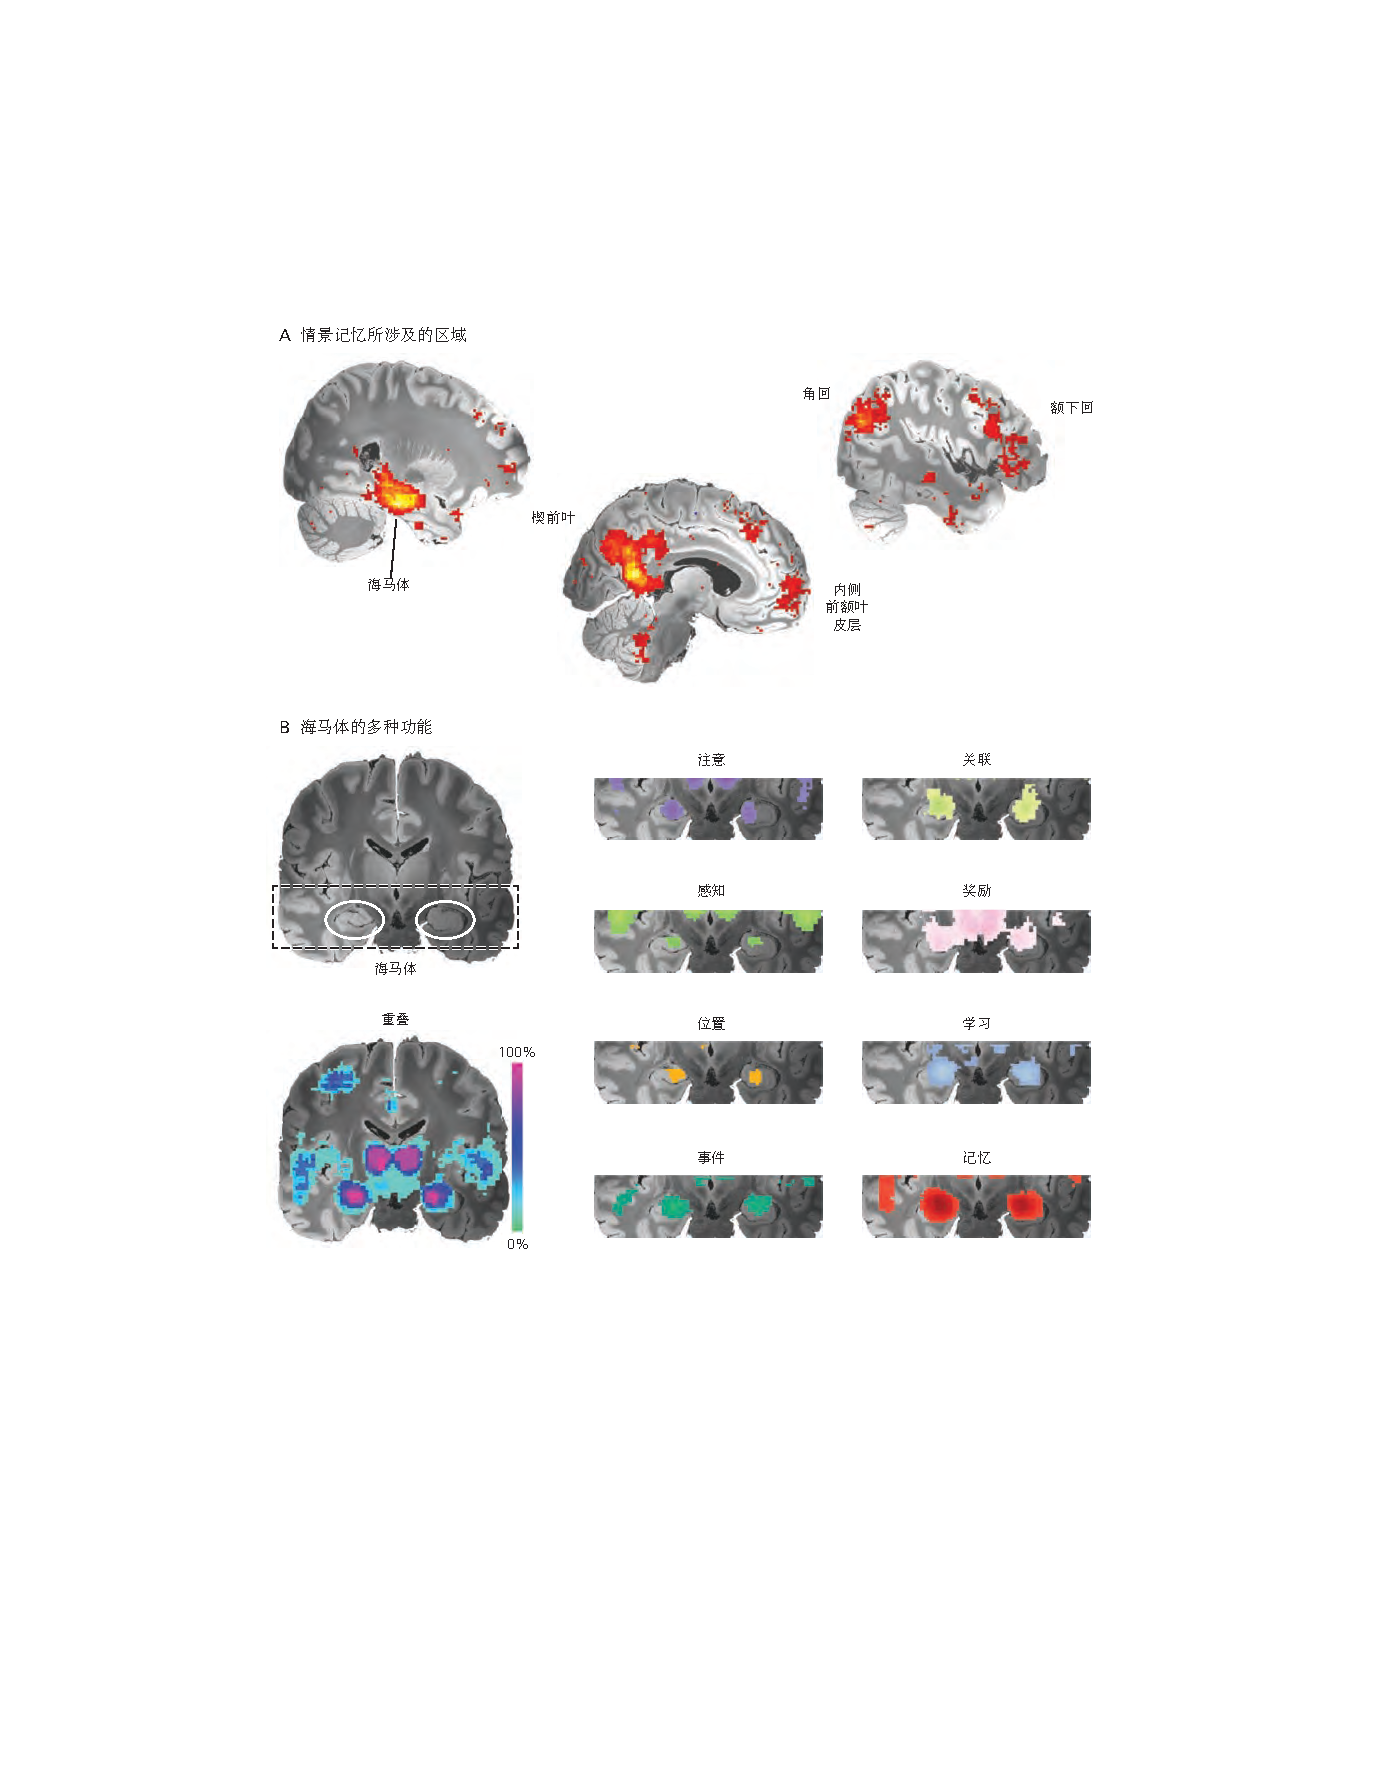
\includegraphics[width=1.0\linewidth]{chap06/fig_6_3}
	\caption{映射思维和大脑的挑战。
		对\textit{功能性核磁共振成像}数据的任何解释都必须考虑认知功能与大脑区域之间关系的复杂性。
		此处通过来自包含 14,000 多项已发表的\textit{功能性核磁共振成像}研究数据库的\textit{元分析}来说明这种复杂性。
		\textbf{A.} 这张地图显示,多个大脑区域参与\textit{情景记忆},即对过去特定事件的编码和检索。
		彩色体素表明在报告这些体素激活的研究中术语“偶发性”的可能性很高(反向推理)。
		这个例子说明了\textit{单个认知功能}如何与\textit{多个大脑区域}相关联(一对多映射)。
		\textbf{B.} 这些图显示海马体参与了多种认知功能(每个半球的白色圆圈)。 
		每个插图大脑中的彩色体素表明这些体素在检查相应术语(前向推理)的研究中被激活的可能性很高。
		重叠图显示了激活每个体素的这些术语的百分比。
		这个例子说明了\textit{单个大脑区域}如何与\textit{多个认知功能}和行为相关联(多对一映射)。}
	\label{fig:6_3}
\end{figure}


% 神经活动 (反向)->心理活动
通过反向推理,神经活动的差异是推断哪个特定心理过程活跃的基础,即使导致差异的条件并非旨在操纵该过程。 
例如,在之前的人脸与非人脸对比中,研究人员可能会将纹状体中的不同活动解释为人脸有益的证据。
这种反向推理通常是不合理的,因为奖励既没有被测量也没有被操纵,即解释是基于其他操纵奖励并发现纹状体活动的研究。
问题的出现是因为每个大脑区域通常支持不止一种功能,这意味着仅通过观察活动就不清楚哪些功能参与了。
事实上,纹状体也与运动密切相关,所以也许面部参与运动而不是奖励过程?
这个例子中逻辑合理的结论反映了前向推理,即纹状体参与了面部识别的某些(尚未解决的)方面。


因此,一种解决方案是不在功能性核磁共振成像研究中使用反向推理。
然而,在某些情况下,反向推理可能是可取的,甚至是必要的。
例如,反向推理可以让研究人员进行探索性分析并生成新的假设,甚至可以从为其他目的收集的数据中得出。
这对于充分利用难以收集的功能性核磁共振成像数据尤其重要,例如来自儿童、老人和患者的数据(方框~\ref{box:6_2})。
出于这种需要,已经开发了统计工具来支持反向推理。
例如,基于网络的工具 Neurosynth 使用已发表研究的大型数据库来分配特定心理过程(例如奖励)的概率,因为在特定区域(例如纹状体)中观察到了血氧水平依赖活动。


\begin{proposition}[现实世界中的大脑成像] \label{box:6_2}
	
	\quad \quad 利用非侵入性工具对人脑进行成像和测量内部心理过程的能力引起了人们对将功能磁共振成像应用于各种现实世界问题的兴趣,如临床诊断和治疗、法律和司法、人工智能、营销和经济以及政治。
	
	\quad \quad 在临床领域,一个有趣的方向是使用功能磁共振成像来检查植物人状态的患者。
	研究表明,一些这样的患者表现出反映心理处理的大脑活动。
	例如,患者可能表现为昏迷(无意识、非交流和对外部刺激不反应),但当被要求思考一个动作时,运动皮层或当被要求想象特定的视觉线索时,在特定类别的视觉区域表现出神经活动。
	这些发现可能会影响临床医生对患者的预后和治疗。
	
	\quad \quad \textit{功能性核磁共振成像}在现实世界中的另一个潜在应用是测谎。
	根据大脑活动准确区分真相和谎言的能力在法庭上可能具有重要价值。
	一些实验室研究报告称,当一组受试者被要求重复撒谎时,大脑活动会有所不同。
	然而,为了有用,功能磁共振成像需要以一种不受策略或对策影响的方式,提供高度可靠的证据,证明一个人是否在特定事件上撒谎。
	这在目前是不可能的,事实上,功能磁共振成像的证据在法庭上通常是不可接受的。
	
	\quad \quad 功能磁共振成像的这些和其他应用引起了道德和隐私方面的担忧。
	例如,当局可以使用功能磁共振成像数据来证明相应的决定(如有罪或无罪),利用公众的偏见来相信生物学解释,即使基础科学尚未确定。
	更令人不安的是,人类目前对我们是否分享内心想法和感受拥有自主权,但感知这些信息的设备可能会改变这一点。
	因此,神经科学家在考虑实际应用时面临的一个重要挑战是准确地传达功能磁共振成像功能强大但有局限性,以及我们对人脑的理解正在进行中。
	
\end{proposition}


区分大脑活动与行为的相关性与大脑活动与行为之间的因果关系也很重要。
如果大脑区域有选择地并持续地参与特定的心理过程,则这种相关性并不能得出它在该过程中发挥必要或充分作用的结论。
% 没有充分性:脑区的激活 不能充分 说明 功能
关于充分性,大脑区域可能(并且很可能确实)与一个或多个其他大脑区域合作以完成该过程。
% 没有必要性
就必要性而言,该地区的活动可能是其他地方加工的次要副产品。


支持功能性核磁共振成像研究解释的一种方法是评估研究结果如何与更具侵入性的方法(例如癫痫患者的电刺激)的研究结果趋同。
由于每种工具都有局限性,包括神经元记录等其他相关措施,因此这种汇聚证据的原则对于推进对大脑如何支持行为的理解至关重要。
除了通过研究和工具汇集证据外,还有人正在努力使用经颅磁刺激或实时神经反馈与功能性核磁共振成像同时操纵大脑功能。




\section{未来的进步取决于技术和概念的进步}

功能性核磁共振成像是迄今为止我们探测健康人脑的最佳技术。
它允许以相当高的分辨率测量整个大脑以及大型受试者样本中心灵的许多方面而不会造成伤害。
然而,从其他方面来说,如果我们想要更深入、更准确地了解大脑的工作原理,它远非我们最终需要的。
与动物可用的工具相比,功能性核磁共振成像提供相对嘈杂、缓慢和间接的神经元活动和回路动力学测量。


正在努力从技术和生物学上解决这些限制。
在技术方面,\textit{多波段成像序列}可以通过并行采集大脑的多个切片来提高\textit{功能性磁共振成像}数据的时间分辨率和空间分辨率。
然而,更快的测量本质上受到\textit{血液动力学反应速度慢}的限制,较小的体素仍然平均分布在数十万个神经元中。


在生物学方面,我们对血氧水平依赖活动如何从大脑的生理机制中产生有了初步的了解,例如单个神经元活动、群体活动、星形胶质细胞和其他神经胶质细胞的功能、神经调节系统和血管系统。
更好地理解\textit{血氧水平依赖}活动与这些过程之间的关系对于了解不同类型的测量何时以及为何一致和分歧至关重要。 
虽然一些实验条件会导致神经元活动和血氧水平依赖活动增加,但其他实验条件不会。
例如,虽然视觉提示的呈现增加了视觉皮层中的血流量和神经元放电,但如果高度期望的这种视觉提示没有呈现,则血流量仍会增加但神经元活动不会增加。
这表明神经活动和血管活动的耦合存在重要的细微差别,这些细微差别可能具有功能意义,并且血管信号本身可能比以前认为的更复杂。


正如功能性核磁共振成像的历史所示,一个领域的科学发现可以导致其他领域的意外突破。
1970 年代核磁共振成像的发现(20 年后导致了 功能性核磁共振成像)来自物理和化学,并且影响深远,以至于\textit{保罗$\cdot$劳特布尔}和\textit{彼得$\cdot$曼斯菲尔德}获得了 2003 年诺贝尔生理学或医学奖。
几十年前核磁共振的发现又使这成为可能,\textit{伊西多$\cdot$拉比}获得了 1944 年的诺贝尔物理学奖,\textit{费利克斯$\cdot$布洛赫}和\textit{爱德华$\cdot$珀塞尔}获得了 1952 年的诺贝尔物理学奖。
这些发现最初与神经科学并无关联,但却引发了心智、大脑和行为研究领域的一场革命。


\section{亮点}

1. 认知神经科学中的功能性大脑成像方法旨在记录与人类大脑中展开的心理过程相关的大脑活动,将\textit{生物学}和\textit{行为测量}联系起来。
目前,占主导地位的技术是功能性核磁共振成像。


2. 功能性核磁共振成像基于两个主要概念:磁共振物理学和神经血管耦合生物学。
结合起来,\textit{功能性核磁共振成像}可以测量\textit{血氧水平依赖}对神经元活动的响应。
当人类受试者在功能性核磁共振成像期间执行认知任务时,随着时间的推移,血氧水平依赖活动的测量可以与特定的心理过程和行为联系起来。

3. 血氧水平依赖活动和行为之间的联系是通过一系列预处理步骤和统计分析推断出来的。
这些分析可以回答一系列问题,例如哪些大脑区域在特定任务期间处于活动状态,哪些信息被编码在区域内活动的空间模式中,以及区域如何作为网络的一部分随着时间的推移相互影响。


4. 人脑成像导致了对许多领域行为的神经机制的基本见解。
一些突出的例子是了解人脑如何处理面孔,如何存储和检索记忆,以及我们如何从反复试验中学习。
在这些领域中,来自功能性核磁共振成像的数据与动物神经元记录的发现以及计算模型的理论预测相融合,提供了大脑与思维之间关系的更完整画面。


5. 功能性核磁共振成像记录大脑活动但不直接修改活动。
因此,它不支持推断某个大脑区域是否是行为所必需的,而是该区域是否与该行为有关。
大多数研究支持对这种参与的前向推论,即大脑中的活动可以与心理过程联系起来,因为实验操纵了该过程。


6. 功能性核磁共振成像提供了一个机会来研究人类大脑的功能,因为它参与了健康和疾病中的各种心理过程。 
这项技术及其生成的数据分析正在不断发展,以提高生物测量的时间分辨率和空间分辨率,并阐明这些测量、心理过程和行为之间的联系。



\chapter*{第二部分:神经系统细胞的细胞生物学和分子生物学}
\markboth{神经系统细胞的细胞生物学和分子生物学}{神经系统细胞的细胞生物学和分子生物学}

\begin{figure}[htbp]
	\centering
	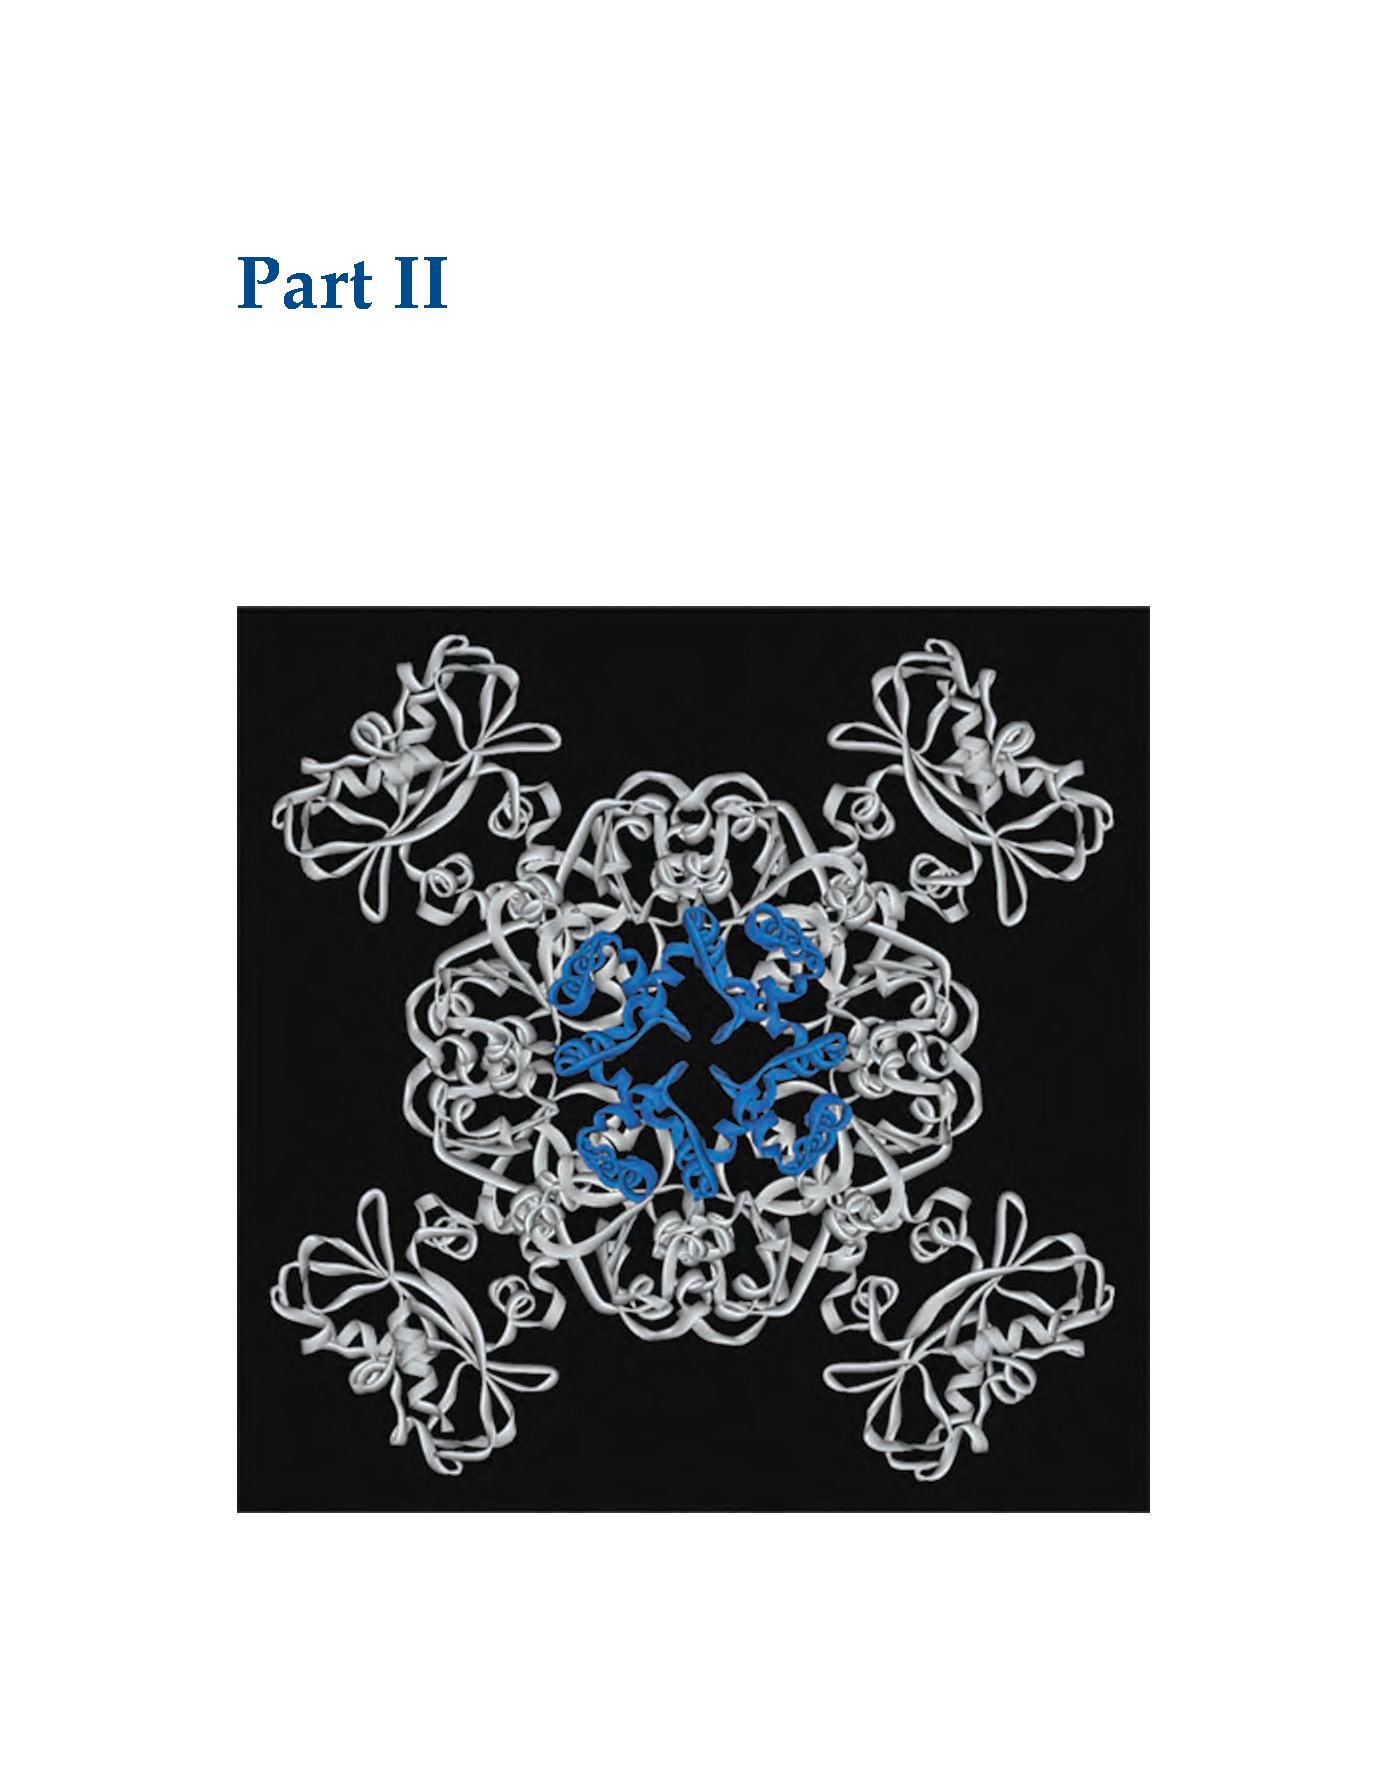
\includegraphics[width=0.9\linewidth]{chap07/fig_7_0}
	\caption{嗜热微生物古甲烷杆菌的MthK \ce{Ca^2+}调节\ce{K+}通道的晶体结构。
		这是从处于\ce{Ca^2+}结合开放状态的通道的细胞外侧观察的。
		MthK由两个主要的功能结构域组成。
		一种完整的膜蛋白形成一个水性孔(蓝色),它选择并传导\ce{K+}离子,并具有一个在打开和关闭构象之间切换的门;
		细胞内\ce{Ca^2+}结合门控环(灰色)控制该门。
		当它结合\ce{Ca^2+}时,所产生的构象变化被机械地传递到孔中,导致其切换到开放状态。}
	\label{fig:7_0}
\end{figure}


在所有的生物系统中,从最原始到最先进,基本的组成部分都是细胞。
细胞通常被组织成在复杂的生物系统中重复的功能模块。
脊椎动物的大脑是模块化系统中最复杂的例子。
复杂的生物系统还有另一个基本特征:
它们是建筑学的——也就是说,它们的解剖结构、精细结构和动态特性都反映了特定的生理功能。
因此,大脑的结构及其组成细胞的细胞生物学、生物物理学和生物化学反映了其基本功能,即调节行为。


神经系统由神经胶质细胞和神经细胞组成。
早期将神经胶质细胞视为纯粹的结构元件的观点已经被我们目前的理解所取代,即有几种类型的神经胶质细胞,每种都专门调节神经元功能的一个或多个特定方面。
不同种类的神经胶质细胞在促进和引导神经发育、隔离轴突过程、控制细胞外环境、支持突触传递、促进学习和记忆以及调节神经系统内的病理过程方面发挥着重要作用。
一些神经胶质细胞具有神经递质受体和电压门控离子通道,使它们能够相互通信,并与神经元通信,以支持神经元信号传导。


与神经胶质细胞相比,神经细胞的巨大多样性——神经系统模块组装的基本单元——是一个基本细胞计划的变体。
该计划的四个特点使神经细胞具有独特的能力,能够在长距离内精确快速地相互交流。
首先,神经元是极化的,一端有感受性树突,另一端有与突触前终末相连的轴突。
这种函数性质的极化将电压脉冲的主要流动限制在一个方向上。
其次,神经元具有电兴奋性。
它的细胞膜含有特殊的蛋白质——离子通道和受体——允许特定无机离子的流入和流出,从而产生电流,在膜上产生电压信号。
第三,神经元含有蛋白质和细胞器,赋予其特殊的分泌特性,使其能够在突触处释放神经递质。
第四,这种在细胞体及其末端之间长距离快速信号传导的系统是由细胞骨架结构实现的,该结构在较慢的时间尺度上介导各种蛋白质、信使核糖核酸和细胞器在两个隔间之间的有效转运。


在本书的这一部分,我们将关注独特的细胞生物学特性,这些特性使神经元和胶质细胞能够实现其各种特殊功能。
重点将放在离子通道的特性上,离子通道赋予神经元以动作电位的形式产生和传播电信号的能力。
我们从考虑离子通道共享的一般性质开始讨论神经元——选择和传导离子的能力,以及在开放和闭合构象之间进行门控的能力。
神经元使用四大类通道进行信号传导:
(1)静息通道产生静息电位,并成为神经元被动电特性的基础,这些特性决定了突触电位的时间进程、沿树突的分布以及触发动作电位的阈值;
(2) 感觉受体通道对某些感觉刺激作出反应,产生局部受体电位;
(3) 配体门控通道对神经递质作出反应而开放,产生局部突触电位;
以及(4)电压门控通道产生产生自传播动作电位的电流。
在这一部分中,我们主要关注静息和电压门控通道。
在第三部分中,我们更详细地考虑了配体门控通道,以及控制其活性的神经递质和第二信使。
感官刺激激活的通道将在第四部分中进行检查。




\chapter{神经系统的细胞} \label{chap:chap7}

神经系统的细胞——神经元和胶质细胞——与一般细胞有许多共同特征。
然而,神经元具有特殊的天赋,能够与体内远处的其他细胞进行精确、快速的通信。
两个特征赋予了神经元这种能力。


首先,它们具有高度的形态和功能不对称性:神经元的一端有接受树突,另一端有传递轴突。
这种排列是单向神经元信号传导的结构基础。


其次,神经元既可电兴奋又可化学兴奋。
神经元的细胞膜包含特殊的蛋白质——离子通道和受体——它们促进特定无机离子的流动,从而重新分配电荷并产生改变跨膜电压的电流。
这些电荷变化可以沿轴突产生动作电位形式的去极化波,这是信号在神经元内传播的通常方式。
胶质细胞不太容易兴奋,但它们的膜含有促进离子摄取的转运蛋白,以及从细胞外空间去除神经递质分子的蛋白质,从而调节神经元功能。


根据树突形态、轴突投射模式和电生理特性,有数百种不同类型的神经元。
这种结构和功能多样性主要由每种神经元细胞类型表达的基因决定。
尽管神经元都继承了相同的基因组,但每个神经元都表达一组受限的基因,因此只产生某些分子——酶、结构蛋白、膜成分和分泌产物——而不是其他分子。
在很大程度上,这种表达取决于细胞的发育历史。
从本质上讲,每个细胞都是它所表达的分子集合。


神经胶质细胞的种类也很多,可以根据其独特的形态、生理和生化特征进行鉴定。
神经胶质细胞的不同形态表明神经胶质细胞可能与神经元一样异质。
尽管如此,脊椎动物神经系统中的胶质细胞可分为两大类:大胶质细胞和小胶质细胞。
大胶质细胞主要分为三种类型:少突胶质细胞、雪旺细胞和星形胶质细胞。
在人脑中,大约 90\% 的胶质细胞是大胶质细胞。
其中,大约一半是髓鞘生成细胞(少突胶质细胞和雪旺细胞),一半是星形胶质细胞。
少突胶质细胞为中枢神经系统中某些神经元的轴突提供绝缘髓鞘(图~\ref{fig:7_1})。 
雪旺细胞使周围神经系统中神经元的轴突形成髓鞘(图 ~\ref{fig:7_1}B);
非髓鞘化雪旺细胞具有其他功能,包括促进神经肌肉突触的发育、维持和修复。
星形胶质细胞因其不规则的大致星形细胞体和大量突起而得名;
它们支持神经元并以多种方式调节神经元信号(图 ~\ref{fig:7_1}C)。 
小胶质细胞是大脑的常驻免疫细胞和吞噬细胞,但在健康大脑中也具有稳态功能。


\begin{figure}[htbp]
	\centering
	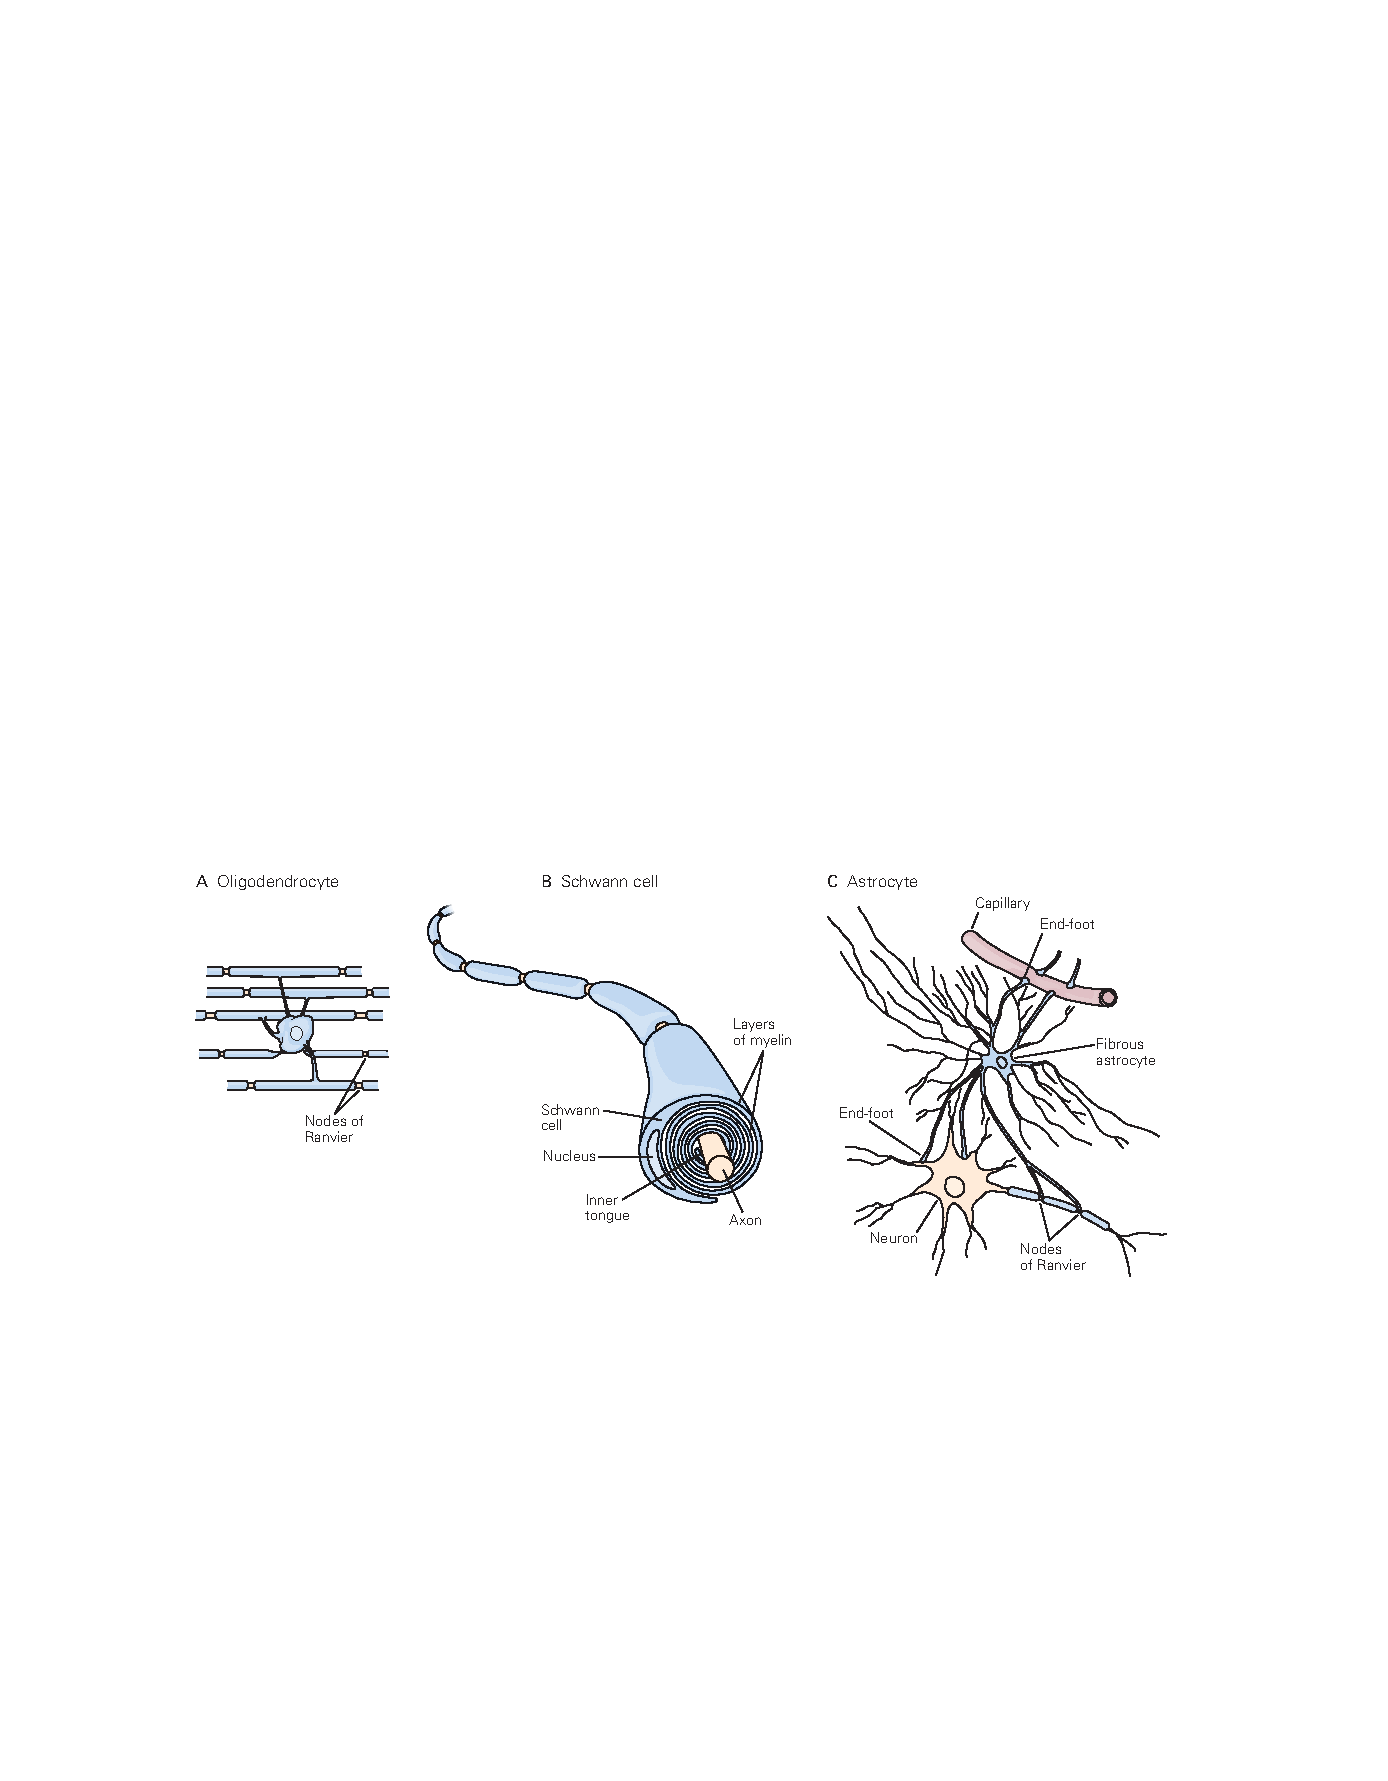
\includegraphics[width=1.0\linewidth]{chap07/fig_7_1}
	\caption{神经胶质细胞的主要类型是中枢神经系统中的少突胶质细胞和星形胶质细胞以及周围神经系统中的雪旺细胞。
		A. 少突胶质细胞是突起相对较少的小细胞。
		如图所示,在大脑的白质中,它们提供了隔离轴突的髓鞘。
		单个少突胶质细胞可以将其膜状突起包裹在许多轴突周围。 在灰质中,神经周围少突胶质细胞包围并支持神经元的细胞体。 B. Schwann 细胞为周围神经系统中的轴突提供髓鞘。 在发育过程中,几个雪旺细胞沿着单个轴突的长度定位。 每个细胞在 Ranvier 的两个节点之间形成一个大约 1 毫米长的髓鞘。 当雪旺细胞的内舌围绕轴突旋转数圈时,鞘形成,将轴突包裹在膜层中。 实际上,髓磷脂层比这里显示的更紧凑。 (改编自 Alberts 等人,2002 年。)C. 星形胶质细胞是中枢神经系统中的一类主要神经胶质细胞,其特征在于其星形形状和突起上的宽端足。 因为这些末端足使星形胶质细胞与毛细血管和神经元接触,所以星形胶质细胞被认为具有营养功能。 星形胶质细胞在维持血脑屏障方面也起着重要作用(在本章后面描述)。}
	\label{fig:7_1}
\end{figure}


\section{神经元和胶质细胞具有许多结构和分子特征}

神经元和胶质细胞从胚胎神经系统的共同神经上皮祖细胞发育而来,并具有许多结构特征(图~\ref{fig:7_2})。
这些细胞的边界由细胞膜或质膜界定,其具有所有生物膜的不对称双层结构,并提供对大多数水溶性物质不可渗透的疏水屏障。
细胞质有两个主要成分:细胞质和膜状细胞器。


\begin{figure}[htbp]
	\centering
	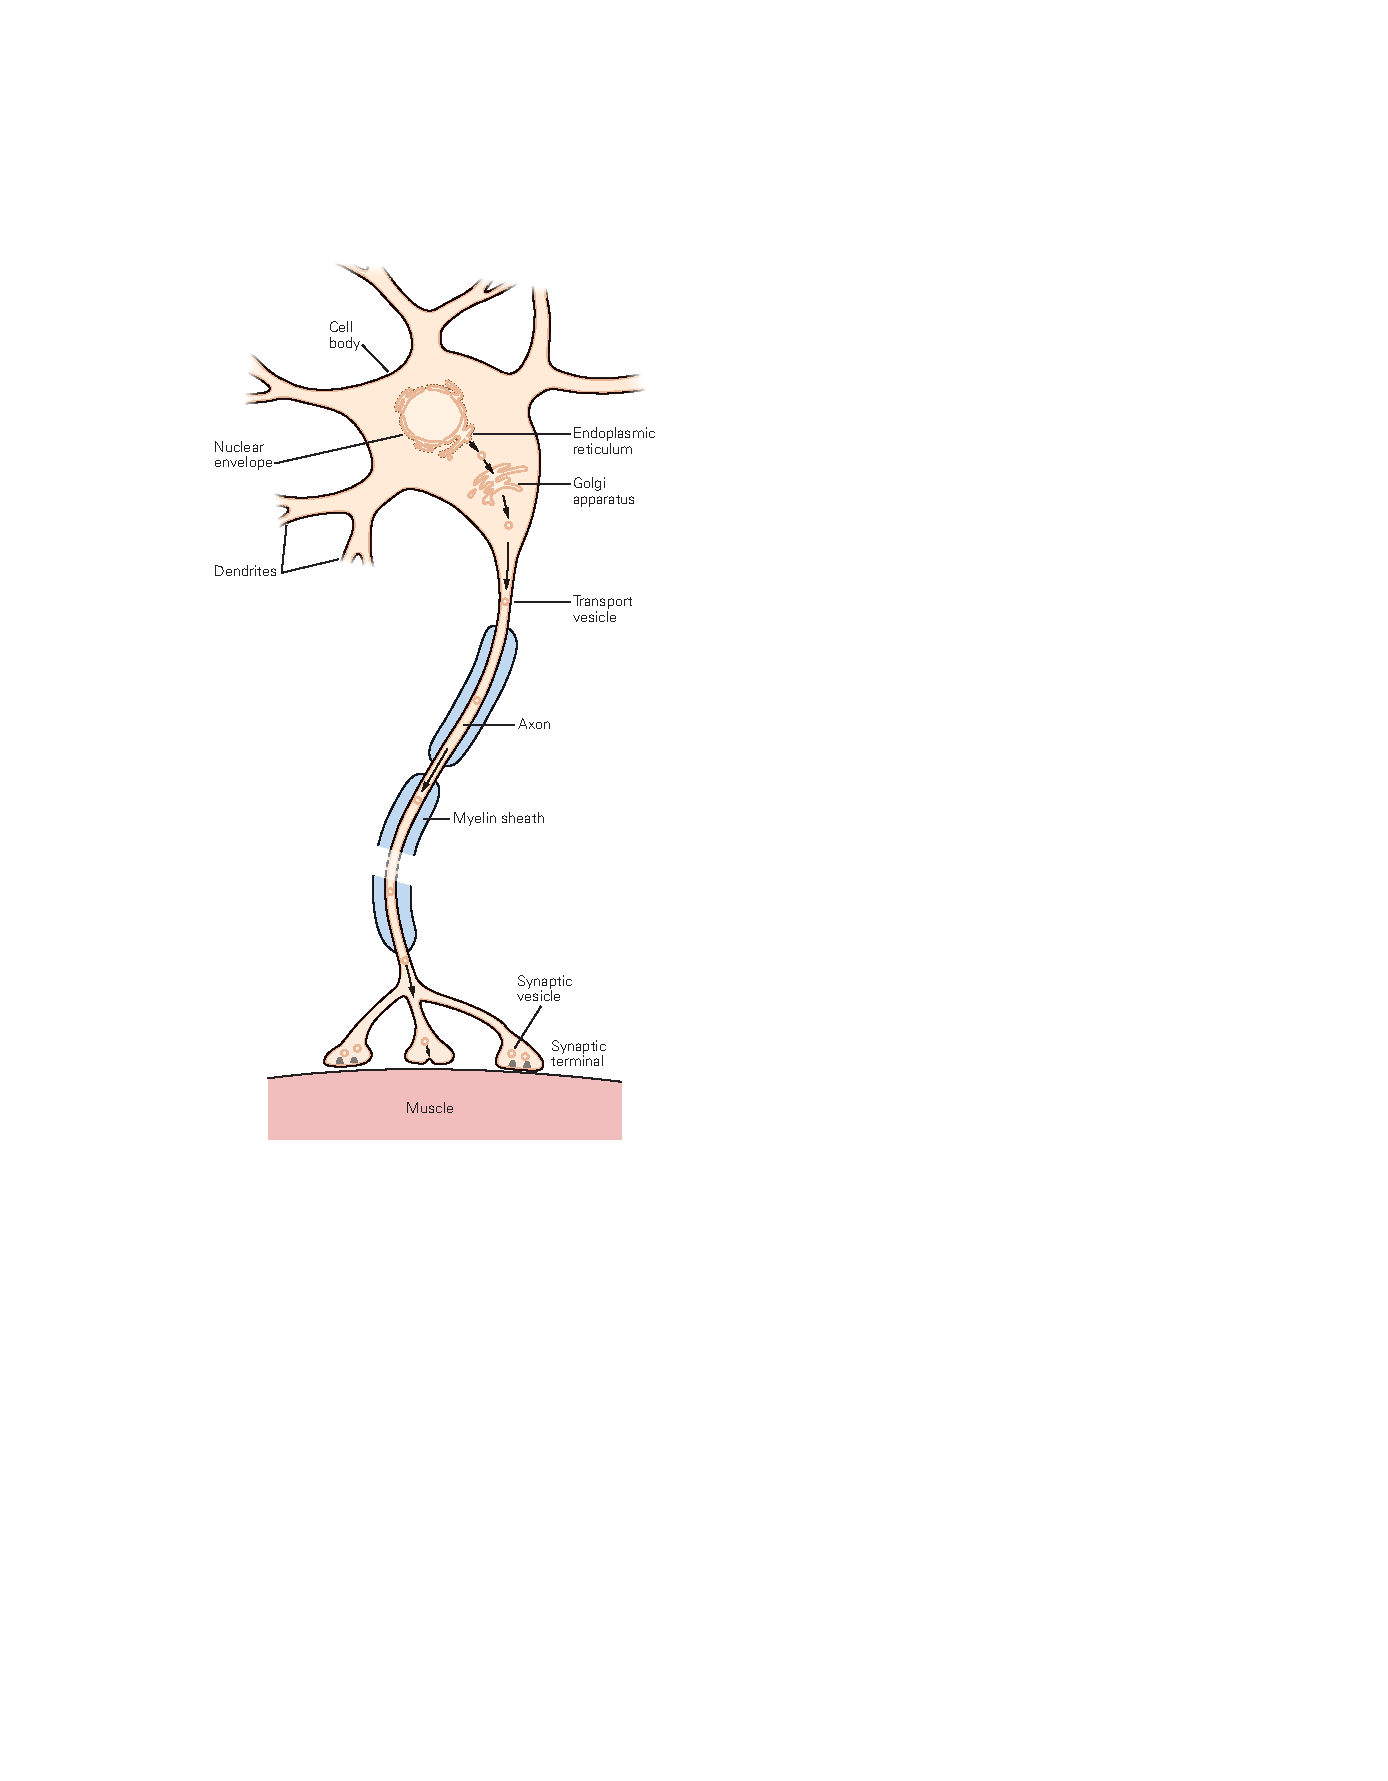
\includegraphics[width=0.5\linewidth]{chap07/fig_7_2}
	\caption{神经元的结构。
		脊髓运动神经元的细胞体和细胞核被双层膜包围,即核膜,与内质网相连。
		构成核膜的两个膜层之间的空间与内质网的腔连续。 树突从神经元的基底面出现,轴突从顶端面出现\cite{williams1989bannister}。}
	\label{fig:7_2}
\end{figure}


胞质溶胶是细胞质的水相。
在此阶段,实际上只有少数蛋白质游离在溶液中。
除了一些催化代谢反应的酶外,大多数蛋白质都被组织成功能复合物。
最近一个叫做蛋白质组学的分支学科已经确定这些复合物可以由许多不同的蛋白质组成,其中没有一个与另一个共价连接。
例如,\textit{N-甲基-D-天冬氨酸}型谷氨酸受体(一种介导中枢神经系统兴奋性突触传递的膜相关蛋白)的细胞质尾部锚定在由 100 多种支架蛋白组成的大型复合体中, 蛋白质修饰酶。
(许多参与第二信使信号转导的胞质蛋白,将在后面的章节中讨论,它们嵌入质膜正下方的细胞骨架基质中。)核糖体是翻译\textit{信使核糖核酸}分子的细胞器,由几个蛋白质亚基组成。
蛋白酶体是一种大型多酶细胞器,可降解泛素化蛋白质(本章稍后描述的过程),它也存在于神经元和胶质细胞的胞质溶胶中。


膜细胞器是细胞质的第二个主要成分,包括线粒体和过氧化物酶体,以及由小管、囊泡和称为液泡器的池组成的复杂系统。
线粒体和过氧化物酶体处理分子氧。
线粒体产生三磷酸腺苷 (ATP),这是细胞能量转移或消耗的主要分子,而过氧化物酶体可防止强氧化剂过氧化氢的积累。
线粒体源自在进化早期侵入真核细胞的共生古细菌,在功能上与液泡器不连续。
线粒体还在钙离子稳态和脂质生物合成中发挥其他重要作用。


液泡器包括光滑内质网、粗面内质网、高尔基复合体、分泌小泡、核内体、溶酶体,以及连接这些不同隔室的多种运输小泡(图~\ref{fig:7_3})。
它们的管腔在拓扑上对应于细胞的外部;
因此,它们脂质双层的内层小叶对应于质膜的外层小叶。


\begin{figure}[htbp]
	\centering
	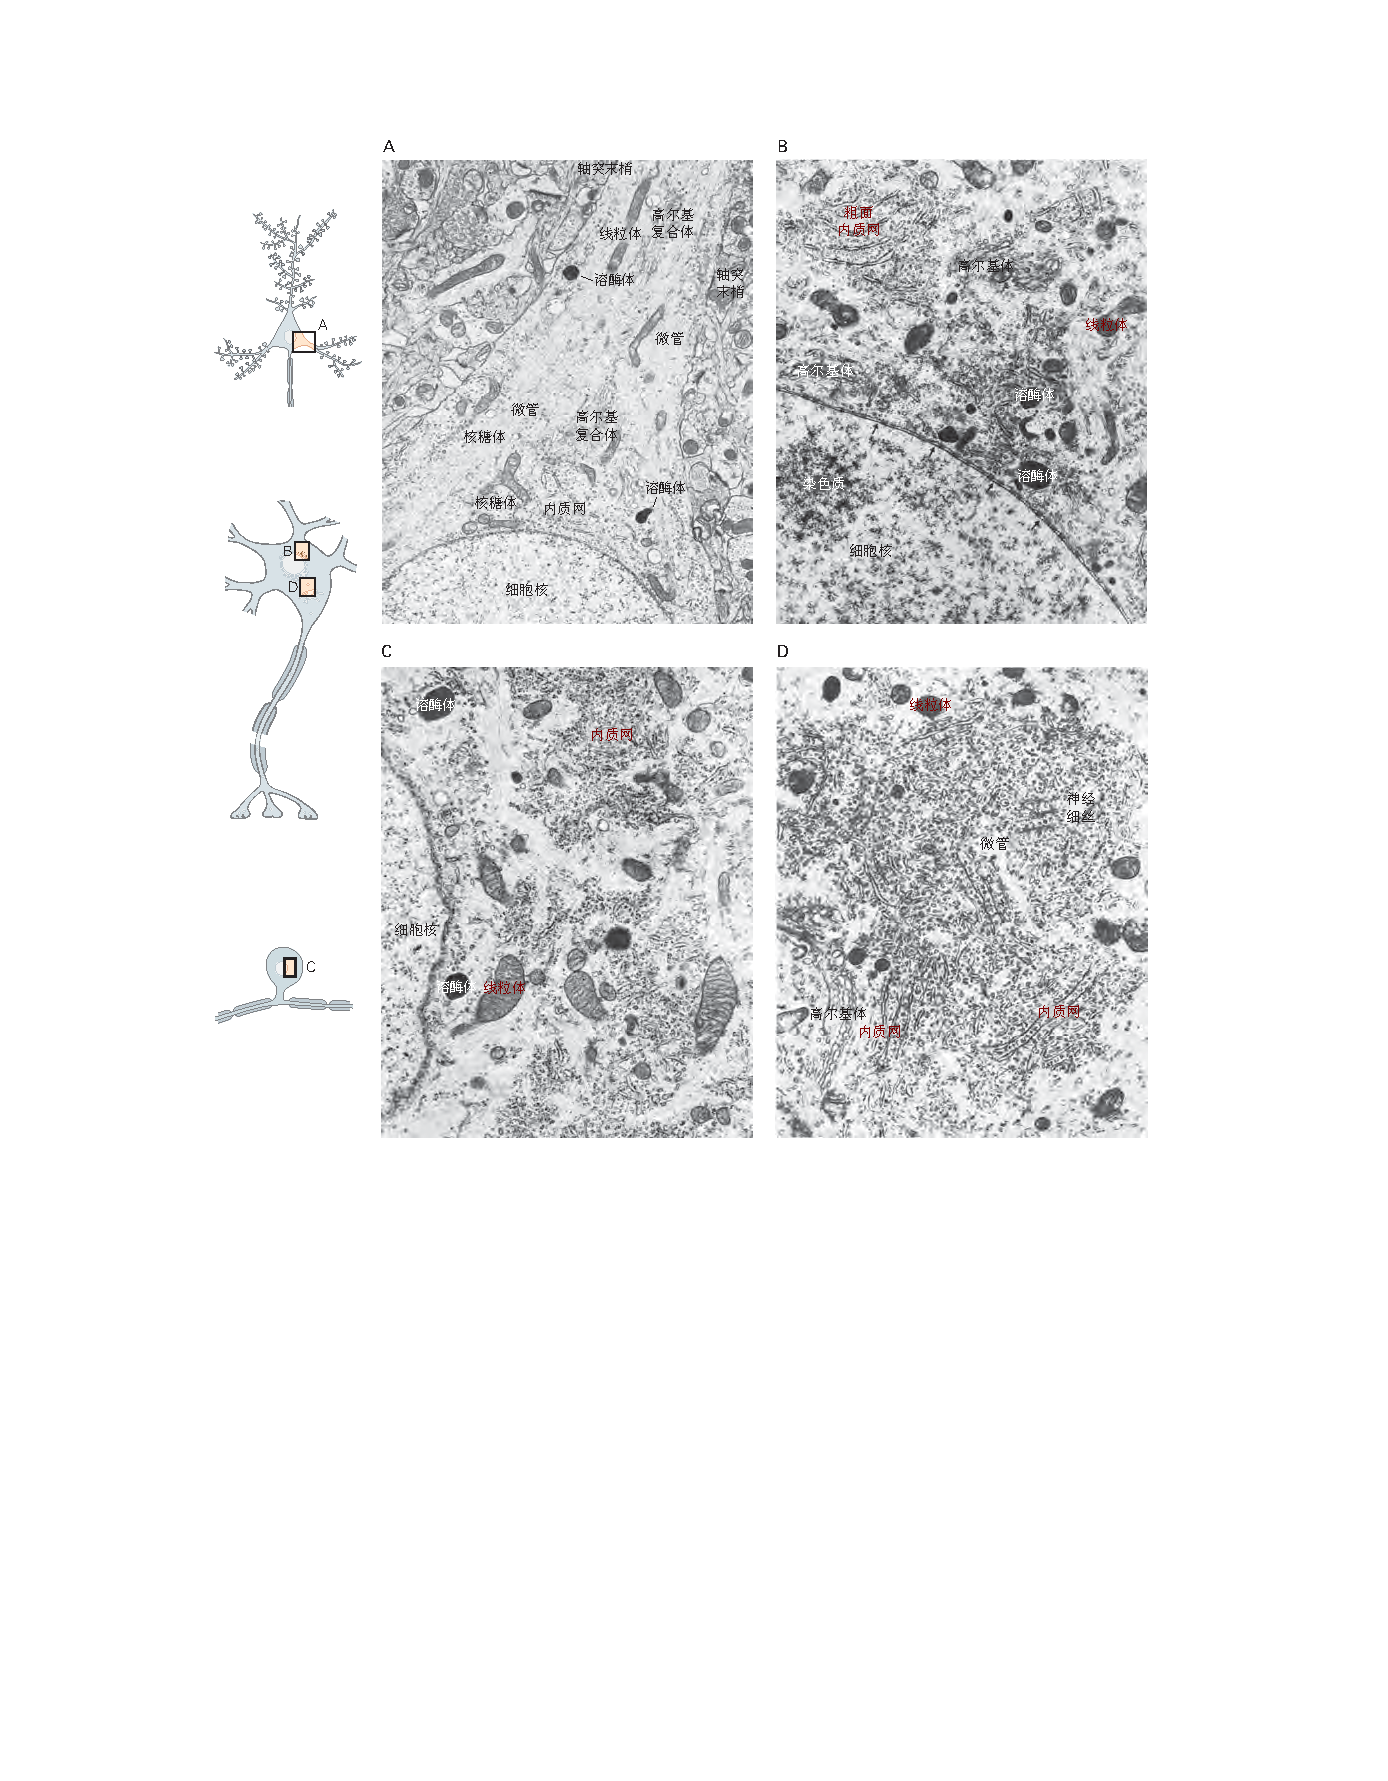
\includegraphics[width=1.0\linewidth]{chap07/fig_7_3}
	\caption{神经元的细胞器。
		电子显微照片显示神经元四个不同区域的细胞质\cite{peters1991neuropil}。
		\textbf{A.} 树突从锥体神经元的细胞体中出现,其中包括细胞核 (N) 上方的内质网 (ER) 和高尔基复合体 (G) 的一部分 附近。
		一些高尔基池已进入树突,线粒体 (Mit)、溶酶体 (Ly) 和核糖体 (R) 也已进入。
		微管 (Mt) 是细胞质中突出的细胞骨架丝。
		在顶部和右侧可以看到与树突接触的轴突末端 (AT)。
		\textbf{B.} 参与大分子合成的脊髓运动神经元的某些成分。 细胞核 (N) 含有大量染色质 (Ch),并以含有许多核孔(箭头)的核膜为界。
		\textit{信使核糖核酸}通过这些孔离开细胞核并附着在核糖体上,核糖体在细胞质中保持游离状态或附着在内质网膜上形成粗面内质网 (RER)。
		细胞质中合成的调节蛋白通过孔进入细胞核。 可以看到高尔基体 (G) 的几个部分,以及溶酶体 (Ly) 和线粒体 (Mit)。
		C、D. 背根神经节细胞 (C) 和运动神经元 (D) 的显微照片显示了细胞体中主要负责蛋白质合成和加工的细胞器。
		\textit{信使核糖核酸}通过核膜进入细胞质并被翻译成蛋白质。 游离多核糖体,即附着在单个\textit{信使核糖核酸}上的一串核糖体,产生胞质蛋白和被导入线粒体 (Mit) 和过氧化物酶体中的蛋白。
		多核糖体附着于内质网 (ER) 膜后,会形成以内质网为目的地的蛋白质。
		此处显示的运动神经元的特定区域还包括高尔基体 (G) 的膜,其中进一步处理膜和分泌蛋白。
		一些新合成的蛋白质在小泡中离开高尔基体,小泡沿着轴突向下移动到突触;
		其他膜蛋白被掺入溶酶体 (Ly) 和其他膜细胞器中。
		微管 (M) 和神经丝 (Nf) 是细胞骨架的组成部分。}
	\label{fig:7_3}
\end{figure}


该系统的主要子隔室在解剖学上是不连续的,但在功能上是相连的,因为膜状和腔内物质通过运输囊泡从一个隔室移动到另一个隔室。
例如,在粗面内质网(布满核糖体的网状部分)和光滑内质网中合成的蛋白质和磷脂被运送到高尔基复合体,然后运送到分泌囊泡,当囊泡膜与 质膜(称为胞吐作用的过程)。
这种分泌途径将膜成分添加到质膜,并将这些分泌囊泡的内容物释放到细胞外空间。


相反,细胞膜的成分通过内吞囊泡进入细胞(内吞作用)。
这些被纳入早期内体,分选集中在细胞外围的隔室。
内吞膜通常含有特定的蛋白质,如跨膜受体,可以通过成熟为循环核内体而直接回到质膜,也可以成熟为晚期核内体,后者通过与溶酶体融合而被靶向降解。
(胞吐作用和胞吞作用将在本章后面详细讨论)平滑内质网还充当整个神经元细胞质中受调节的内部钙离子储存(参见第~\ref{chap:chap14} 章中关于\ce{Ca^2+} 释放的讨论)。


粗面内质网的一个特殊部分形成了核包膜,这是一个球形扁平池,围绕着染色体\textit{脱氧核糖核酸}及其相关蛋白(组蛋白、转录因子、聚合酶和异构酶)并定义了细胞核(图~\ref{fig:7_3})。 
因为核包膜与内质网的其他部分和液泡器的其他膜是连续的,所以推测它已经进化为质膜的内陷以包裹真核染色体。
核膜被核孔打断,核膜的内外膜融合导致亲水通道的形成,蛋白质和\textit{核糖核酸}通过该通道在细胞质本身和核细胞质之间交换。


尽管核质和细胞质是细胞质的连续结构域,但只有分子量小于 5,000 的分子才能通过扩散自由地穿过核孔。
较大的分子需要帮助。
一些蛋白质具有特殊的核定位信号,这些区域由一系列基本氨基酸(精氨酸和赖氨酸)组成,可被称为核输入受体 (importins) 的可溶性蛋白质识别。
在核孔中,这种复合物被另一组称为核孔蛋白的蛋白质引导进入细胞核。


神经细胞体的细胞质延伸到树突状树中,没有功能分化。 
通常,细胞体细胞质中的所有细胞器也存在于树突中,尽管粗面内质网、高尔基复合体和溶酶体的密度随着与细胞体的距离而迅速减小。 
在树突中,光滑的内质网在称为棘的细突底部突出(图 ~\ref{fig:7_4}~和~\ref{fig:7_5}),这是兴奋性突触的接受部分。
树突棘中多聚核糖体的浓度介导局部蛋白质合成(见下文)。


\begin{figure}[htbp]
	\centering
	\includegraphics[width=0.7\linewidth]{chap07/fig_7_4}
	\caption{高尔基体和内质网膜从细胞体延伸到树突中。
		\textbf{A.} 高尔基体复合体(实线箭头)在光学显微镜下显示为数条伸入树突(空心箭头)但未伸入轴突的细丝。
		底部的箭头表示轴突小丘。
		对于这张显微照片,脑干的一个大神经元用专门针对高尔基复合体的抗体进行了免疫染色\cite{de1986heterogeneous}。
		\textbf{B.} 光滑的内质网(箭头)延伸到树突棘的颈部,而另一个膜室位于脊柱的起点 (箭)\cite{cooney2002endosomal}。}
	\label{fig:7_4}
\end{figure}


\begin{figure}[htbp]
	\centering
	\includegraphics[width=1.0\linewidth]{chap07/fig_7_5}
	\caption{树突棘的类型。
		海马 CA1 区锥体细胞的成熟树突显示三种类型的树突棘形状。
		左图基于一系列电子显微照片\cite{harris1989dendritic,sorra1993occurrence}。
		位于突触前轴突对面的表面(箭头)包含突触受体。
		此处以及 B 和 C 中显示的组织来自出生后第 15 天大鼠大脑的海马体。
		\textbf{B.} 含有突触后密度(箭头)的粗短棘在成熟的海马体中既小又罕见。
		它们较大的对应物(未显示)在未成熟的大脑中占主导地位。
		\textbf{C.} 蘑菇形刺的头部较大。 此处显示的未成熟脊柱包含平滑内质网的扁平池,一些具有串珠外观(实线箭头)。 空心箭头表示突触后密度。}
	\label{fig:7_5}
\end{figure}


与细胞体和树突的连续性相反,轴突出现的轴突小丘处的细胞体之间存在明显的功能边界。
构成神经元中蛋白质主要生物合成机制的细胞器——核糖体、粗面内质网和高尔基复合体——通常被排除在轴突之外(图~\ref{fig:7_4}),溶酶体和某些蛋白质也是如此。
然而,轴突富含光滑内质网、单个突触小泡及其前体膜。



\section{细胞骨架决定细胞形状}

细胞骨架决定细胞的形状,并负责细胞质内细胞器的不对称分布。
它包括三种丝状结构:微管、神经丝和微丝。 
这些细丝和相关蛋白约占细胞总蛋白的四分之一。


微管形成长支架,从神经元的一端延伸到另一端,在发育和维持细胞形状方面发挥关键作用。
单个微管可以长达 0.1 毫米。
微管由原丝组成,每个原丝由多对沿微管纵向排列的 a-和 b-微管蛋白亚基组成(图~\ref{fig:7_6}A)。 
微管蛋白亚基沿原丝与相邻的亚基结合,并在相邻原丝之间横向结合。
微管用正端(或生长端)和负端(微管可以解聚的地方)极化。
有趣的是,轴突和树突之间的微管方向不同。
在轴突中,微管显示单一方向,正端远离细胞体。
在近端树突中,微管可以双向定向,正端朝向或远离细胞体。


\begin{figure}[htbp]
	\centering
	\includegraphics[width=1.0\linewidth]{chap07/fig_7_6}
	\caption{纤维结构图谱。
		\textbf{A.} 微管是最大直径的纤维 (25 纳米),是由 13 根原丝组成的螺旋圆柱体,每根原丝的宽度为 5 纳米。
		每个原丝由一列交替的 $\alpha$-和$\beta$-微管蛋白亚基组成;
		每个亚基的分子量约为 50,000 Da。
		相邻的亚基沿纵向原丝相互结合,并在相邻原丝的亚基之间横向结合。
		微管蛋白分子是由一个 $\alpha$- 和一个 $\beta$- 微管蛋白亚基组成的异二聚体。
		1. 微管视图。
		箭头指示右手螺旋的方向。
		2. 微管的侧视图显示交替的 α 和 β 亚基。
		\textbf{B.} 神经丝由相互缠绕的纤维构成,以产生厚度增加的线圈。
		最薄的单元是形成卷曲螺旋异二聚体的单体。
		这些二聚体形成成为原丝的四聚体复合物。
		两个原纤维变成一个原纤维,三个原纤维螺旋扭曲形成直径 10 纳米的神经丝\cite{bershadsky2012cytoskeleton}。
		\textbf{C.} 微丝是直径最小的纤维(约 7 纳米),由排列成螺旋状的两股聚合球状肌动蛋白 (G-actin) 单体组成。
		在哺乳动物中至少发现了六种不同(但密切相关)的肌动蛋白; 每个变体都由一个单独的基因编码。
		微丝是极性结构,因为球状单体是不对称的。}
	\label{fig:7_6}
\end{figure}


微管通过在其正端添加三磷酸鸟苷 (GTP) 结合的微管蛋白二聚体而生长。
聚合后不久,GTP 被水解为二磷酸鸟苷 (GDP)。
当微管停止生长时,其正端被 GDP 结合的微管蛋白单体所覆盖。
GDP 结合的微管蛋白对聚合物的低亲和力会导致灾难性的解聚,这并不是因为微管通过与其他蛋白质的相互作用而稳定。


事实上,虽然微管在分裂细胞中经历聚合和解聚的快速循环,这种现象被称为动态不稳定,但在成熟的树突和轴突中,它们更稳定。
这种稳定性被认为是由促进微管蛋白聚合物定向聚合和组装的微管相关蛋白 (MAP) 引起的。
轴突中的 MAP 不同于树突中的 MAP。
例如,MAP2 存在于树突中,但不存在于轴突中,轴突中存在 tau 蛋白(见方框~\ref{box:7_1})和 MAP1b。
此外,微管稳定性也受到许多不同类型的可逆微管蛋白翻译后修饰的严格调节,例如乙酰化、去酪氨酸化和聚谷氨酰化。
在阿尔茨海默病和其他一些退行性疾病中,tau 蛋白被修饰并异常聚合,形成一种称为神经原纤维缠结的特征性损伤(方框~\ref{box:7_1})。


\begin{proposition}[神经解剖学导航术语] \label{box:7_1}
	
	\quad \quad 蛋白质的异常积累是许多神经系统疾病的标志。
	
	\quad \quad Tau是一种微管结合蛋白,通常存在于神经细胞中。在阿尔茨海默病中,在光学显微镜下,神经元、神经胶质细胞以及细胞外空间中都可以看到tau的异常聚集。
	排列在细长聚合物中的高度磷酸化的tau分子相互缠绕,形成成对的螺旋丝(图~\ref{fig:7_7}A和第~\ref{chap:chap64}~章)。
	被称为神经原纤维缠结的聚合物束聚集在神经元细胞体、树突和轴突中(图~\ref{fig:7_7}A)。
	
	\quad \quad 在正常神经元中,tau要么与微管结合,要么在胞质溶胶中游离。
	在缠结中,它不与微管结合,但高度不溶。缠结的形成至少部分是因为tau没有被蛋白水解降解。
	堆积物干扰微管蛋白的聚合,从而干扰轴突运输。
	因此,神经元的形状没有得到维持。
	
	\quad \quad 在进行性核上性麻痹(一种运动障碍)患者和额颞叶痴呆(一组影响额叶和颞叶的神经退行性疾病)患者的神经元中也发现了Tau积聚(第~\ref{chap:chap63}~章)。
	额颞叶痴呆的家族形式是由tau基因突变引起的。在进行性核上性麻痹、皮质-基底神经节变性和额颞叶痴呆的星形胶质细胞和少突胶质细胞中也发现异常聚集体。
	
	\quad \quad β淀粉样蛋白肽也在阿尔茨海默病的细胞外空间积聚(图~\ref{fig:7_7}B和第~\ref{chap:chap64}~章)。
	它是一种更大的整体膜蛋白淀粉样蛋白前体蛋白的小蛋白水解产物,通常由与细胞内膜相关的几种蛋白水解酶处理。
	产生β-淀粉样蛋白的蛋白水解途径需要β-分泌酶。
	
	\quad \quad 由于未知的原因,在阿尔茨海默病中,异常量的淀粉样蛋白前体由β-分泌酶处理。
	一些早发性家族性阿尔茨海默病患者的淀粉样蛋白前体基因或编码膜蛋白早老素1和2的基因发生突变,这些基因与分泌酶活性密切相关。
	
	\quad \quad 在帕金森病中,α-突触核蛋白的异常聚集体在神经元的细胞体中积累。与tau一样,a-突触核蛋白是细胞的一种正常可溶性成分。但在帕金森病中,它变得不溶,形成称为路易体的球形内含物(图~\ref{fig:7_7}C和第~\ref{chap:chap63}~章)。
	
	\quad \quad 这些异常内含物也含有泛素。由于泛素是蛋白质蛋白酶体降解所必需的,它的存在表明受影响的神经元试图靶向α-突触核蛋白或其他分子成分进行蛋白水解。
	显然,降解不会发生,可能是因为蛋白质的错误折叠或异常聚集,或者是因为细胞中错误的蛋白水解处理。
	
	\quad \quad 这些异常的蛋白质积累会影响神经元和神经胶质细胞的生理机能吗?
	一方面,积累可以响应蛋白质的翻译后处理的改变而形成,并用于分离异常蛋白质,从而允许正常的细胞活动。
	另一方面,这些积累可能会破坏细胞活动,如膜运输、轴突和树突运输,以及特定类别神经元之间突触连接的维持。
	此外,除了聚集之外,改变的蛋白质本身可能具有有害影响。
	对于β-淀粉样蛋白,有证据表明该肽本身具有毒性。
	
\end{proposition}


\begin{figure}[htbp]
	\centering
	\includegraphics[width=0.7\linewidth]{chap07/fig_7_7}
	\caption{阿尔茨海默病和帕金森病神经元内蛋白质的异常聚集。
	\textbf{A.} 左图:阿尔茨海默病的细胞内神经原纤维缠结,此处用暗银染色。(经J.P.Vonsatel许可复制。)
	右图:缠结的电子显微照片显示,异常细丝成束,充满树突。
	细丝由改变的tau蛋白组成。(经英国威克福德Runwell医院的L.Carrasco医生许可使用。)
	\textbf{B.} 在阿尔茨海默病中,淀粉样斑块是由聚合的β-淀粉样肽的细胞外沉积形成的。此处显示的斑块有一个致密的淀粉样蛋白核心,以及周围的沉积物晕。斑块中的一些神经元过程表现出缠结病理。
	\textbf{C.} 帕金森病患者黑质中的路易体含有由α-突触核蛋白和其他蛋白质组成的异常细丝。}
	\label{fig:7_7}
\end{figure}


微管蛋白由多基因家族编码。 
至少有六个基因编码 α 和 β 亚基。 
由于不同基因的表达或转录后修饰,大脑中存在 20 多种微管蛋白亚型。


直径为 10 nm 的神经丝是细胞骨架的骨骼(图 ~\ref{fig:7_6} B)。
神经丝与其他细胞类型的中间丝有关,包括上皮细胞(头发和指甲)的细胞角蛋白、星形胶质细胞中的神经胶质原纤维酸性蛋白和肌肉中的结蛋白。
与微管不同,神经丝是稳定的并且几乎完全聚合在细胞中。


微丝的直径为 3 至 7 nm,是构成细胞骨架的三种主要纤维类型中最细的(图~\ref{fig:7_6} C)。 
与肌肉的细丝一样,微丝由两股聚合的球状肌动蛋白单体组成,每条单体都带有 ATP 或二磷酸腺苷 (ADP),缠绕成双链螺旋。
肌动蛋白是所有细胞的主要成分,可能是自然界中最丰富的动物蛋白。
有几种密切相关的分子形式:骨骼肌的 α 肌动蛋白和至少两种其他分子形式,β 和 γ。
每个都由不同的基因编码。
高等脊椎动物的神经肌动蛋白是 β 和 γ 种类的混合物,它与肌肉肌动蛋白的区别在于几个氨基酸残基。 
大多数肌动蛋白分子是高度保守的,不仅在一个物种的不同细胞类型中,而且在人类和原生动物等远亲生物中也是如此。


与微管和神经丝不同,肌动蛋白丝很短。
它们集中在质膜下方的皮质细胞质中的细胞外围,在那里它们与许多肌动蛋白结合蛋白(例如,spectrinfodrin、ankyrin、talin 和 actinin)形成致密网络。 
该基质在细胞外围的动态功能中起着关键作用,例如发育过程中生长锥(轴突的生长尖端)的运动、细胞表面特化微区的产生以及突触前和突触后形态的形成 专长。


与微管一样,微丝经历聚合和解聚循环。
在任何时候,细胞中总肌动蛋白的大约一半可以作为未聚合的单体存在。
肌动蛋白的状态由结合蛋白控制,结合蛋白通过覆盖快速生长的细丝末端或切断它来促进组装并限制聚合物长度。 
其他结合蛋白交联或束缚肌动蛋白丝。
微管和微丝的动态状态允许成熟的神经元收缩旧的轴突和树突并延伸新的。
这种结构可塑性被认为是突触连接和功效变化的主要因素,因此也是长期记忆和学习的细胞机制。



\section{蛋白质颗粒和细胞器沿轴突和树突主动运输}

在神经元中,大多数蛋白质是在细胞体中由\textit{信使核糖核酸}制成的。
重要的例子是神经递质生物合成酶、突触小泡膜成分和神经分泌肽。
由于轴突和末端通常距离细胞体很远,因此维持这些偏远区域的功能是一项挑战。
被动扩散速度太慢,无法在这么远的距离内输送囊泡、颗粒,甚至单个大分子。


轴突末端是神经递质的分泌部位,离细胞体特别远。
在支配人类腿部肌肉的运动神经元中,神经末梢与细胞体的距离可以超过细胞体直径的 10,000 倍。
因此,细胞体内形成的膜和分泌产物必须主动运输到轴突末端(图~\ref{fig:7_9})。


\begin{figure}[htbp]
	\centering
	\includegraphics[width=0.5\linewidth]{chap07/fig_7_9}
	\caption{神经元中的膜运输。 1. 分泌细胞器的蛋白质和脂质在内质网中合成并转运到高尔基复合体,在那里组装大的致密核心囊泡(含肽分泌颗粒)和突触囊泡前体。 2. 大的致密核心囊泡和运输囊泡通过轴突运输将突触囊泡蛋白沿轴突向下传送。 3. 在神经末梢,突触小泡组装并装载非肽类神经递质。 突触小泡和大的致密核小泡通过胞吐作用释放其内容物。 4. 胞吐作用后,大的致密核囊泡膜返回细胞体以供再利用或降解。 突触小泡膜在突触前末梢经历多次局部胞吐和胞吞循环。}
	\label{fig:7_9}
\end{figure}


1948 年,Paul Weiss 在绑扎坐骨神经时首次展示了轴突运输,并观察到神经中的轴浆在结扎线的近端随时间积累。
他得出结论,在他称之为轴浆流的过程中,轴浆以缓慢、恒定的速度从细胞体向末端移动。
今天我们知道,Weiss 观察到的流动由两种不同的机制组成,一种快,另一种慢。


膜状细胞器通过快速轴突运输向轴突末端(顺行方向)移动并返回细胞体(逆行方向),这种运输形式在温血动物中每天高达 400 毫米。
相比之下,细胞溶质和细胞骨架蛋白仅通过更慢的运输形式(轴突运输)沿顺行方向移动。
神经元中的这些传输机制是对促进所有分泌细胞中细胞器细胞内运动的过程的适应。
因为所有这些机制都沿着轴突运作,神经解剖学家已经使用它们来追踪单个轴突的过程以及神经元之间的相互联系(方框~\ref{box:7_2})。

\begin{proposition}[神经解剖学追踪利用轴突运输] \label{box:7_2}
	
	\quad \quad 神经解剖学家通常通过微量注射染料来定位特定神经细胞体的轴突和末梢;
	荧光蛋白的表达;或在给予放射性标记的氨基酸、某些标记的糖(岩藻糖或氨基糖,糖蛋白的前体)或特异性递质物质后不久用放射自显影法追踪特异性蛋白质。
	
	\quad \quad 类似地,通过内吞作用在神经末梢容易被吸收并转运回细胞体的颗粒、蛋白质或染料被用于识别细胞体。
	辣根过氧化物酶在这类研究中被最广泛地使用,因为它很容易进行逆行运输,并且其反应产物可以方便地用组织化学方法观察。
	
	\quad \quad 轴突运输也被神经解剖学家用来标记神经元之间交换的物质,从而有可能识别神经元网络(图~\ref{fig:7_10})。
	
\end{proposition}


\begin{figure}[htbp]
	\centering
	\includegraphics[width=1.0\linewidth]{chap07/fig_7_10}
	\caption{单纯疱疹病毒(HSV)的轴索转运被用来追踪猴子的皮层通路。根据毒株的不同,病毒通过轴突运输沿顺行或逆行方向移动。
		在任何一个方向上,它都会进入一个神经元,受感染的细胞与该神经元进行突触接触。
		在这里,使用顺行移动菌株(HSV-1[H129])追踪猴子初级运动皮层中的细胞向小脑的投射。
		猴子被注射到控制手臂的初级运动皮层区域。
		4天后,对大脑进行切片并对病毒抗原进行免疫染色。
		显微照片显示,病毒从初级运动皮层转移到桥核的二阶神经元(A),然后转移到小脑皮层的三阶神经元(B)。}
	\label{fig:7_10}
\end{figure}



\subsection{快速轴突运输携带膜细胞器}

大型膜状细胞器通过快速运输进出轴突末端(图 ~\ref{fig:7_11})。
这些细胞器包括突触小泡前体、大的致密核心小泡、线粒体、光滑内质网的元素和携带\textit{核糖核酸}的蛋白质颗粒。
直接显微分析表明,快速运输沿着与轴突主轴对齐的微管线性轨道以停止和启动(跳跃式)的方式发生。
运动的跳跃性质是由于细胞器从轨道上周期性解离或与其他粒子的碰撞造成的。


\begin{figure}[htbp]
	\centering
	\includegraphics[width=1.0\linewidth]{chap07/fig_7_1}
	\caption{早期关于顺行轴突运输的实验使用了蛋白质的放射性标记。
		在此处说明的实验中,在将 [3H]-亮氨酸注射到脊髓腰部背根神经节后的不同时间测量了放射性蛋白沿猫坐骨神经的分布。
		为了在一张图中显示不同时间(注射后 2、4、6、8 和 10 小时)的传输曲线,使用了多个纵坐标标度(以对数单位表示)。
		大量标记蛋白留在神经节细胞体中,但随着时间的推移,沿着坐骨神经中的轴突移出,因此标记蛋白的前进前沿逐渐远离细胞体(箭头)。
		运输速度可以根据不同时间前沿的距离来计算。
		通过此类实验,西德尼·奥克斯 (Sidney Ochs) 发现,在体温下,轴突快速运输的速度恒定为每天 410 毫米\cite{ochs1972fast}。}
	\label{fig:7_11}
\end{figure}


背根神经节细胞的早期实验表明,顺行快速转运严重依赖于 ATP,不受蛋白质合成抑制剂的影响(一旦注射的标记氨基酸被掺入),并且不依赖于细胞体,因为它发生在轴突中 从他们的细胞体中分离出来。
事实上,主动运输可以发生在重组的无细胞轴浆中。


微管提供了一个基本固定的轨道,分子马达可以在该轨道上移动特定的细胞器。
微管参与快速转运的想法源于以下发现:某些破坏微管和阻断依赖于微管的有丝分裂的生物碱也会干扰快速转运。


分子马达首先在电子显微照片中显示为微管和运动粒子之间的交叉桥(图~\ref{fig:7_8})。
更先进的荧光延时显微镜技术能够可视化特定货物(如线粒体和突触小泡)的轴突运输动力学。
用于顺行运输的运动分子是称为驱动蛋白和多种驱动蛋白相关蛋白的加端定向运动。
驱动蛋白代表一大类腺苷三磷酸酶 (ATPase),每一种都运输不同的货物。
驱动蛋白是由两条重链和两条轻链组成的异四聚体。
每条重链具有三个结构域:(1) 一个球状头部(ATPase 结构域),当连接到微管时充当马达,(2) 一个卷曲螺旋茎,负责与另一条重链二聚化,以及 (3) 与轻链相互作用的扇形羧基末端。
复合物的这一端间接连接到细胞器,细胞器通过称为货物适配器的特定蛋白质家族移动。


\begin{figure}[htbp]
	\centering
	\includegraphics[width=1.0\linewidth]{chap07/fig_7_8}
	\caption{轴突的细胞骨架结构。
		显微照片显示了由交叉桥(箭头)连接的微管和神经丝的密集堆积。
		细胞器在富含微管的区域中沿顺行和逆行方向运输。
		显微照片中的可视化是通过快速冷冻和深度蚀刻实现的\cite{schnapp1982cytoplasmic}。
		M,髓鞘; MT,微管。 ×105,000。}
	\label{fig:7_8}
\end{figure}


快速逆行运输主要移动由神经末梢、线粒体和内质网元件的内吞活动产生的核内体。
许多这些成分通过与溶酶体融合而被降解。
快速逆行运输还传递调节神经元细胞核中基因表达的信号。
例如,神经末梢处激活的生长因子受体被吸收到囊泡中,并沿着轴突运回细胞核。
转录因子的转运通知细胞核中的基因转录装置周围的条件。
这些分子的逆行运输在神经再生和轴突再生过程中尤为重要(第~\ref{chap:chap47}~章)。 
某些毒素(破伤风毒素)以及病原体(单纯疱疹病毒、狂犬病病毒和脊髓灰质炎病毒)也沿着轴突向细胞体输送。


逆行快速运输的速度大约是顺行快速运输的二分之一到三分之二。
与顺行运输一样,颗粒在逆行流动期间沿着微管移动。
逆行轴突运输的马达分子是负端定向马达,称为动力蛋白,类似于在非神经元细胞的纤毛和鞭毛中发现的马达。 它们由一个多聚体 ATPase 蛋白复合物组成,两个球状头部位于连接到基础结构的两个茎上。
球形头部附着在微管上并充当马达,向聚合物的负端移动。
与驱动蛋白一样,复合体的另一端通过专门的货物适配器连接到运输的细胞器上。


微管还介导由 RNA 结合蛋白形成的颗粒携带的\textit{信使核糖核酸}和核糖体\textit{核糖核酸}的顺行和逆行运输。
这些蛋白质已在脊椎动物和无脊椎动物神经系统中得到表征,包括细胞质聚腺苷酸化元件结合蛋白 (CPEB)、脆性 X 蛋白、Hu 蛋白、NOVA 和 Staufen。
这些蛋白质的活性至关重要。
例如,CPEB 在从细胞体到神经末梢的运输过程中使选定的\textit{信使核糖核酸}保持休眠状态;
一旦到达那里(受到刺激),结合蛋白可以通过介导聚腺苷酸化和信使激活来促进\textit{核糖核酸}的局部翻译。
CPEB 和 Staufen 都是在果蝇中发现的,它们在未受精卵中保持母体\textit{信使核糖核酸}休眠,并在受精后将\textit{信使核糖核酸}分布和定位到分裂胚胎的各个区域。
脆性 X (FMR1) 基因的功能缺失突变会导致严重的精神发育迟滞。


蛋白质、核糖体和\textit{信使核糖核酸}集中在一些树突棘的底部(图~\ref{fig:7_12})。
只有一组选定的\textit{信使核糖核酸}从胞体转运到树突中。
这些包括编码肌动蛋白和细胞骨架相关蛋白、MAP2 和钙离子/钙调蛋白依赖性蛋白激酶的 α 亚基的\textit{信使核糖核酸}。
它们在树突中翻译以响应突触前神经元中的活动。
这种局部蛋白质合成被认为对于维持作为长期记忆和学习基础的突触分子变化很重要。
同样,髓鞘碱性蛋白的\textit{信使核糖核酸}被运送到少突胶质细胞的远端,在那里它随着髓鞘的生长而被翻译,这将在本章后面讨论。


\begin{figure}[htbp]
	\centering
	\includegraphics[width=0.5\linewidth]{chap07/fig_7_12}
	\caption{树突状乔木中的核糖体。 (图像经 Oswald Steward 许可转载。) A. 一些核糖体从细胞体分派到树突,在那里它们用于局部蛋白质合成。 这张放射自显影图显示了\textit{核糖体核糖核酸}在使用原位杂交的低密度培养物中海马神经元中的分布。 该图像是用暗场照明制作的,其中银颗粒反射光线,因此看起来像亮点。 表示 rRNA 的银粒高度集中在细胞体和树突上,但在树突之间纵横交错的轴突上检测不到。 B. 树突中的核糖体选择性地集中在脊柱和主树突轴(箭头)的交界处,在这里脊柱接触突触前神经元的轴突末端。 这张电子显微照片显示了海马齿状回中一个神经元的蘑菇状脊柱。 注意树突轴中没有核糖体。 S,脊柱头; T,突触前末梢; Den,包含长线粒体的树突的主轴。 ×60,000。}
	\label{fig:7_12}
\end{figure}


\subsection{缓慢的轴突运输携带细胞溶质蛋白和细胞骨架的元素}

细胞溶质蛋白和细胞骨架蛋白通过缓慢的轴突运输从细胞体中移出。
慢转运只发生在顺行方向,由至少两个以不同速率携带不同蛋白质的动力学成分组成。


较慢的成分每天移动 0.2 至 2.5 毫米,并携带构成细胞骨架纤维状元素的蛋白质:神经丝的亚基和微管的 α- 和 β- 微管蛋白亚基。
这些纤维蛋白约占较慢成分中移动的总蛋白的 75\%。 
微管通过涉及微管滑动的机制以聚合形式运输,其中相对较短的预组装微管沿着现有微管移动。
神经丝单体或短聚合物与微管一起被动移动,因为它们通过蛋白质桥交联。


缓慢轴突运输的另一个组成部分的速度大约是较慢部分的两倍。
它携带网格蛋白、肌动蛋白和肌动蛋白结合蛋白以及多种酶和其他蛋白质。



\section{与其他分泌细胞一样,蛋白质也是在神经元中制造的}

\subsection{分泌蛋白和膜蛋白在内质网中合成和修饰}

分泌蛋白和膜蛋白的\textit{信使核糖核酸}通过粗面内质网膜翻译,其多肽产物在内质网腔内广泛加工。
大多数注定要成为蛋白质的多肽在合成过程中会跨过粗面内质网膜,这一过程称为共翻译转移。


转移是可能的,因为核糖体,蛋白质合成的位点,附着在网状细胞的胞质表面(图~\ref{fig:7_13})。 
多肽链完全转移到网状细胞腔中会产生一种分泌蛋白(回想一下,网状细胞的内部与细胞的外部有关)。
重要的例子是神经活性肽。
如果转移不完全,则会产生完整的膜蛋白。
由于多肽链在合成过程中可以多次穿过膜,因此根据蛋白质的一级氨基酸序列,可能有几种跨膜构型。
重要的例子是神经递质受体和离子通道(第 ~\ref{chap:chap8}~章)。


\begin{figure}[htbp]
	\centering
	\includegraphics[width=1.0\linewidth]{chap07/fig_7_13}
	\caption{}
	\label{fig:7_13}
\end{figure}


一些运输到内质网中的蛋白质保留在那里。
其他的则移动到液泡器的其他隔室或质膜,或分泌到细胞外空间。
在内质网中加工的蛋白质被广泛修饰。
一个重要的修饰是由成对的游离巯基侧链氧化引起的分子内二硫键 (Cys-S-S-Cys) 的形成,这一过程不能发生在胞质溶胶的还原环境中。
二硫键对于这些蛋白质的三级结构至关重要。


蛋白质可以在合成过程中(共翻译修饰)或之后(翻译后修饰)被胞质酶修饰。
一个例子是 N-酰化,将酰基转移到生长中的多肽链的 N-末端。
14-碳脂肪酸肉豆蔻酰基的酰化允许蛋白质通过脂质链锚定在膜中。


其他脂肪酸可以与半胱氨酸的巯基结合,产生硫酰化作用:

异戊二烯化是另一种翻译后修饰,对于将蛋白质锚定到细胞膜的胞质侧很重要。
它在蛋白质合成完成后不久发生,涉及一系列酶促步骤,导致巯基的两个长链疏水聚异戊二烯基(法尼基,具有 15 个碳原子,或香叶基-香叶基,具有 20 个)之一发生硫代酰化 蛋白质 C 末端的半胱氨酸。


一些翻译后修饰很容易可逆,因此可用于瞬时调节蛋白质的功能。
这些修饰中最常见的是蛋白激酶对丝氨酸、苏氨酸或酪氨酸残基中羟基的磷酸化。
去磷酸化由蛋白磷酸酶催化。 (这些反应在第 ~\ref{chap:chap14}~章中讨论。)与所有翻译后修饰一样,要磷酸化的位点由要修饰的残基周围的特定氨基酸序列决定。
磷酸化可以以可逆的方式改变生理过程。
例如,蛋白质磷酸化-去磷酸化反应调节离子通道的动力学、转录因子的活性和细胞骨架的组装。


另一个重要的翻译后修饰是将泛素(一种具有 76 个氨基酸的高度保守的蛋白质)添加到蛋白质分子中特定赖氨酸残基的ε-氨基上。
调节蛋白质降解的泛素化由三种酶介导。
E1是一种利用ATP能量的活化酶。
激活的泛素接下来被转移到结合酶 E2,然后将激活的部分转移到连接酶 E3。
E3 单独或与 E2 一起将泛素基转移到蛋白质的赖氨酸残基上。
特异性的产生是因为给定的蛋白质分子只能被特定的 E3 或 E3 和 E2 的组合泛素化。
一些 E3 还需要特殊的辅助因子——泛素化仅在 E3 和辅助因子蛋白存在的情况下发生。


单泛素化标记一种蛋白质在内体-溶酶体系统中降解。
这在表面受体的内吞作用和再循环中尤为重要。
泛素基单体依次连接到先前添加的泛素部分中赖氨酸残基的ε-氨基。
在多泛素链上添加超过 5 个泛素,标记蛋白质被蛋白酶体降解,蛋白酶体是一种大型复合物,包含可将蛋白质切割成短肽的多功能蛋白酶亚基。


ATP-泛素-蛋白酶体途径是一种选择性和调节蛋白水解的机制,在神经元所有区域(树突、细胞体、轴突和末端)的胞质溶胶中起作用。
直到最近,这一过程还被认为主要针对折叠不良、变性或老化和受损的蛋白质。
我们现在知道泛素介导的蛋白水解可以受神经元活动的调节,并在许多神经元过程中发挥特定作用,包括突触发生和长期记忆存储。


另一个重要的蛋白质修饰是糖基化,它发生在天冬酰胺残基的氨基上(N-连接糖基化)并导致复杂多糖链的整体添加。
然后,通过伴侣分子控制的一系列反应,包括热休克蛋白、钙联接蛋白和钙网蛋白,这些链在内质网内被修剪。 
由于寡糖部分具有很强的化学特异性,这些修饰对细胞功能具有重要意义。
例如,发育过程中发生的细胞间相互作用依赖于两个相互作用细胞表面糖蛋白之间的分子识别。
此外,由于给定的蛋白质可能具有略微不同的寡糖链,糖基化可以使蛋白质的功能多样化。
它可以增加蛋白质的亲水性(对分泌蛋白有用),微调其结合大分子伙伴的能力,并延缓其降解。


一种有趣的\textit{信使核糖核酸}翻译后修饰是 RNA 干扰 (RNAi),即双链\textit{核糖核酸}的靶向破坏。
这种机制被认为是为了保护细胞免受病毒和其他无赖核酸片段的侵害而产生的,它会关闭任何目标蛋白质的合成。 
双链\textit{核糖核酸}被一种酶复合物吸收,该酶复合物将分子切割成寡聚体。
\textit{核糖核酸}序列被复合物保留。
结果,任何同源杂交\textit{核糖核酸}链,无论是双链还是单链,都将被破坏。
这个过程是再生的:复合物保留一个杂交片段,然后继续破坏另一个\textit{核糖核酸}分子,直到细胞中没有分子为止。
尽管 RNAi 在正常细胞中的生理作用尚不清楚,但将 RNAi 转染或注射到细胞中具有重要的研究和临床意义(第~\ref{chap:chap2}~章)。



\subsection{分泌蛋白在高尔基复合体中被修饰}

来自内质网的蛋白质在运输囊泡中被携带到高尔基复合体,在那里它们被修饰,然后移动到突触末端和质膜的其他部分。
高尔基复合体表现为一组以长带状排列的膜质袋。


从简单的单细胞原核生物(酵母)到多细胞生物体的神经元和胶质细胞,囊泡在分泌和内吞途径站之间运输的机制一直非常保守。
运输囊泡从膜发展而来,首先是在膜的胞质表面的选定斑块处组装形成外壳的蛋白质或外壳蛋白。
外套有两个功能。
它形成刚性笼状结构,使膜外翻成芽状,并选择要掺入囊泡的蛋白质货物。


有几种类型的外套。
网格蛋白涂层有助于在内吞过程中外翻高尔基复合体膜和质膜。
另外两个外壳,COPI 和 COPII,覆盖在内质网和高尔基复合体之间穿梭的运输囊泡。
一旦游离囊泡形成,包衣通常会迅速溶解。
囊泡与靶膜的融合是由一系列分子相互作用介导的,其中最重要的是两个相互作用膜的胞质表面上小蛋白的相互识别:囊泡可溶性 N-乙基马来酰亚胺敏感因子附着蛋白受体 (v-SNAREs) 和 t-SNAREs (targetmembrane SNAREs)。
第~\ref{chap:chap15}~章讨论了 SNARE 蛋白通过突触小泡与质膜融合释放神经递质的作用。


来自内质网的囊泡到达高尔基复合体的顺侧(面向细胞核的一侧)并与其膜融合以将其内容物输送到高尔基复合体中。
这些蛋白质从一个高尔基体隔室(水池)移动到下一个,从顺式到反式,经历一系列酶促反应。
每个高尔基池或一组池专门用于特定类型的反应。
几种类型的蛋白质修饰,其中一些开始于内质网,发生在高尔基复合体本身或与其反侧相邻的运输站内,反式高尔基网络(复合体的一面通常背对细胞核朝向 轴突丘)。
这些修饰包括添加 N-连接寡糖、O-连接(在丝氨酸和苏氨酸的羟基上)糖基化、磷酸化和硫酸化。


穿过高尔基体复合体的可溶性和膜结合蛋白均从跨高尔基体网络出现在各种具有不同分子组成和目的地的囊泡中。 
从跨高尔基体网络转运的蛋白质包括分泌产物以及质膜、核内体和其他膜细胞器的新合成成分(见图~\ref{fig:7_2})。
一类囊泡携带新合成的质膜蛋白和持续分泌的蛋白质(组成型分泌)。
这些囊泡以不受管制的方式与质膜融合。
这些囊泡的一种重要类型将溶酶体酶递送至晚期核内体。


还有其他类型的囊泡携带由细胞外刺激(调节分泌)释放的分泌蛋白。
一种类型以高浓度储存分泌产物,主要是神经活性肽。
由于它们在电子显微镜下的电子致密(亲渗)外观而被称为大的致密核心囊泡,这些囊泡在功能和生物发生方面与内分泌细胞的含肽颗粒相似。
大的致密核心囊泡主要针对轴突,但在神经元的所有区域都可以看到。
它们积聚在质膜正下方的细胞质中,并高度集中在轴突末端,在那里它们的内容物通过钙离子调节的胞吐作用释放。


最近的研究表明,小的突触小泡——负责在轴突末端快速释放神经递质的电子透明小泡——作为单独的货物被积极地运送到突触末端。
据认为,小突触小泡的蛋白质成分源自跨高尔基体网络的大前体小泡。
这些突触小泡已经包含了大部分能够在突触前活动区融合的蛋白质。
存储在这些突触小泡中的神经递质分子通过胞吐作用释放,胞吐作用受钙离子通过靠近释放位点的通道流入的调节。
然后,囊泡会经历第~\ref{chap:chap15}~章所述的循环/胞吐作用循环。
重要的是,这些囊泡通过称为囊泡转运蛋白的专门转运蛋白重新填充,这些转运蛋白对每种神经递质(例如,谷氨酸、γ-氨基丁酸 [GABA]、乙酰胆碱)具有特异性。



\section{表面膜和细胞外物质在细胞内循环}

从质膜到内部细胞器的内吞流量不断平衡流向细胞表面的囊泡流量。
这种流量对于维持膜面积处于稳定状态是必不可少的。
它可以改变细胞表面许多重要调节分子的活性(例如,通过去除受体和粘附分子)。
它还将营养物质和分子(例如可消耗的受体配体和受损的膜蛋白)去除到细胞的降解区室中。
最后,它用于在神经末梢回收突触小泡(第~\ref{chap:chap15}~章)。


很大一部分内吞交通是在网格蛋白包被的囊泡中进行的。 
网格蛋白涂层通过跨膜受体选择性地与将被吸收到细胞中的细胞外分子相互作用。
因此,网格蛋白介导的摄取通常被称为受体介导的内吞作用。
囊泡最终脱落其网格蛋白外壳并与早期核内体融合,在核内体中,将被回收到细胞表面的蛋白质与那些用于其他细胞内细胞器的蛋白质分开。
质膜的斑块也可以通过更大的、未包被的液泡循环,这些液泡也与早期内体融合(大量内吞作用)。



\section{胶质细胞在神经功能中发挥多种作用}

Ramón y Cajal 认识到神经胶质细胞与大脑中的神经元和突触的密切联系(图~\ref{fig:7_14})。 
尽管当时它们的功能还是个谜,但他预测神经胶质细胞的功能肯定不仅仅是将神经元聚集在一起。
事实上,现在很清楚神经胶质细胞在大脑发育、功能和疾病中起着关键作用。


\begin{figure}[htbp]
	\centering
	\includegraphics[width=0.5\linewidth]{chap07/fig_7_14}
	\caption{星形胶质细胞与大脑中的神经元和突触相互作用。 Ramón y Cajal 绘制的这幅图(基于用升华氯化金法染色的组织)显示了人脑中阿蒙角的锥体层和辐射层的星形胶质细胞。
		(A) 一个大的星形胶质细胞包裹着一个锥体神经元。
		(B) 双星形胶质细胞在神经细胞体 (C) 周围形成巢穴。
		其中一个星形胶质细胞发出两个分支以形成另一个巢 (D)。 
		(E) 细胞显示自溶迹象。 (F) 毛细血管。 }
	\label{fig:7_14}
\end{figure}



\subsection{胶质细胞形成轴突的绝缘鞘}

少突胶质细胞和雪旺细胞的主要功能是提供绝缘材料,使电信号能够沿轴突快速传导。
这些细胞产生薄薄的髓磷脂片,多次同心地包裹在轴突周围。
由少突胶质细胞产生的 CNS 髓磷脂与由雪旺细胞产生的周围神经系统髓磷脂相似,但不完全相同。


两种类型的神经胶质细胞都只为部分轴突产生髓磷脂。
这是因为轴突并没有连续包裹在髓鞘中,髓鞘是一种促进动作电位传播的特征(第~\ref{chap:chap9}~章)。 
一个雪旺细胞为一个轴突的一个节段产生一个髓鞘,而一个少突胶质细胞为多达 30 个轴突的节段产生髓鞘(图 ~\ref{fig:7_1}~和~\ref{fig:7_15})。


\begin{figure}[htbp]
	\centering
	\includegraphics[width=1.0\linewidth]{chap07/fig_7_15}
	\caption{神经胶质细胞产生髓磷脂,使中枢神经元和外周神经元的轴突绝缘。
		\textbf{A.} 中枢神经系统的轴突被少突胶质细胞产生的多层髓鞘包裹。
		每个少突胶质细胞可以形成许多轴突\cite{raine1984morphology}。
		\textbf{B.} 这张小鼠坐骨神经轴突 (Ax) 横截面的电子显微照片显示了髓磷脂 (MI) 片层起源于称为内中轴突 (IM) 的结构。
		髓磷脂起源于雪旺细胞的表面膜 (SM),它与外中轴突 (OM) 连续。
		在这张图片中,雪旺细胞的细胞质 (Sc Cyt) 仍然围绕着轴突;
		最终它被挤出,髓鞘层变得紧凑,如 C 部分所示\cite{thomas1984clinical}。
		\textbf{C.} 周围神经纤维在几个阶段被雪旺细胞髓鞘化。
		在第 1 阶段,雪旺细胞围绕着轴突。
		在第 2 阶段,质膜的外部在一个区域变得紧密并置。
		这种膜融合反映了早期髓鞘膜的形成。
		在第 3 阶段,由于雪旺细胞的细胞质围绕轴突持续旋转,已经形成了几层髓鞘。
		第四阶段,成熟的髓鞘已经形成;
		雪旺细胞的大部分细胞质都被挤出了最内层的环\cite{williams1989bannister}。}
	\label{fig:7_15}
\end{figure}


轴突上髓鞘的层数与轴突的直径成正比——较大的轴突具有较厚的鞘。
直径非常小的轴突没有髓鞘;
无髓鞘轴突传导动作电位的速度比有髓鞘轴突慢得多,因为它们的直径较小且缺乏髓鞘绝缘(第~\ref{chap:chap9}~章)。


鞘的规则层状结构和生化成分是神经胶质质膜形成髓磷脂的结果。
在周围神经系统的发育过程中,在髓鞘形成之前,轴突位于雪旺细胞形成的槽内。
雪旺细胞以规则的间隔沿着轴突排列,成为轴突的有髓鞘部分。
每个雪旺细胞的外膜围绕着轴突形成一个双膜结构,称为中轴突,它在同心层中围绕轴突伸长和螺旋(图 ~\ref{fig:7_15}C)。 
当轴突被包裹时,雪旺细胞的细胞质被挤出,形成紧凑的层状结构。


髓鞘的规则间隔部分被无髓鞘间隙隔开,称为朗飞结,其中轴突的质膜暴露于细胞外空间约 1 μm(图 ~\ref{fig:7_16})。 
这种安排极大地提高了神经冲动传导的速度(人类高达 100 m/s),因为信号从一个节点跳到下一个节点,这种机制称为跳跃式传导(第~\ref{chap:chap9}~章)。 
节点很容易兴奋,因为产生动作电位的 \ce{Na+} 通道的密度在节点处的轴突膜中比在膜的髓鞘区域中高大约 50 倍。
节点周围的细胞粘附分子使髓鞘边界保持稳定。


\begin{figure}[htbp]
	\centering
	\includegraphics[width=0.6\linewidth]{chap07/fig_7_16}
	\caption{轴突的髓鞘有规则的间隙,称为郎飞结。
		\textbf{A.} 电子显微照片显示周围神经系统和脊髓轴突中的节点区域。
		轴突 (Ax) 在两张显微照片中都垂直延伸。
		髓鞘 (M) 层在节点 (Nd) 处不存在,轴突膜(轴突膜,Al)暴露在外\cite{peters1991neuropil}。
		\textbf{B.} Ranvier 节点两侧的区域富含髓鞘细胞和轴突之间的稳定接触,以确保节点不会移动或改变大小和 限制轴突中 \ce{K+} 和 \ce{Na+} 通道的定位。
		钾渗透通道和粘附蛋白 Caspr2 集中在 juxtaparanode 中。
		雪旺细胞或少突胶质细胞细胞质的旁节环 (PNL) 与轴突形成一系列稳定的连接。
		副节点区域富含粘附蛋白,如 Caspr2、接触素和神经成束蛋白 (NF155)。
		在中央轴突的节点处,perinodal 星形胶质细胞过程 (PNP) 接触轴突膜,该膜富含 \ce{Na+} 通道。
		\ce{Na+} 渗透性的这种定位是有髓轴突跳跃式传导的主要基础。
		膜细胞骨架接头锚蛋白 G (ankG) 和细胞粘附分子 NrCAM 和 NF186 也集中在节点处\cite{peles2000molecular}。}
	\label{fig:7_16}
\end{figure}


在人类股神经中,初级感觉轴突长约0.5米,节间距离为1至1.5毫米;
因此,大约 300 到 500 个朗飞节点沿着大腿肌肉和背根神经节细胞体之间的初级传入纤维出现。
因为每个节间节段由单个雪旺细胞形成,所以多达 500 个雪旺细胞参与每个外周感觉轴突的髓鞘形成。


髓磷脂具有散布在蛋白质层之间的双分子脂质层。
其成分与质膜相似,由 70\% 的脂质和 30\% 的蛋白质以及高浓度的胆固醇和磷脂组成。
在中枢神经系统中,髓磷脂有两种主要蛋白质:
髓磷脂碱性蛋白,一种位于致密髓磷脂细胞质表面的小的带正电荷的蛋白质,以及蛋白脂质蛋白,一种疏水性整合膜蛋白。
据推测,两者都为护套提供了结构稳定性。



两者也被认为是重要的自身抗原,免疫系统可以针对这些自身抗原产生反应,从而产生脱髓鞘疾病多发性硬化症。 
在周围神经系统中,髓磷脂含有一种主要的蛋白质 P0,以及疏水性蛋白质 PMP22。
对这些蛋白质的自身免疫反应会产生脱髓鞘周围神经病,即吉兰-巴利综合征。
髓鞘蛋白基因的突变也会导致外周和中央轴突发生多种脱髓鞘疾病(方框~\ref{box:7_3})。
脱髓鞘作用减慢甚至停止受影响轴突中动作电位的传导,因为它允许电流从轴突膜泄漏。
因此,脱髓鞘疾病对中枢和外周神经系统的神经回路具有破坏性影响(第~\ref{chap:chap57}~章)。


\begin{proposition}[髓鞘蛋白缺陷破坏神经信号传导] \label{box:7_3}
	
	\quad \quad 因为在有髓鞘轴突中,神经冲动的正常传导取决于髓鞘的绝缘特性,有缺陷的髓鞘会导致运动和感觉功能的严重紊乱。
	
	\quad \quad 许多影响髓鞘的疾病,包括一些脱髓鞘疾病的动物模型,都有遗传基础。
	颤抖(或shi)突变小鼠有震颤和频繁抽搐,往往英年早逝。
	在这些小鼠中,中枢神经系统中轴突的髓鞘形成严重不足,并且确实发生的髓鞘形成是异常的。
	
	\quad \quad 导致这种疾病的突变是位于小鼠18号染色体上的髓鞘碱性蛋白基因的六个外显子中的五个缺失。突变是隐性的;
	只有从父母双方遗传了缺陷基因,老鼠才会患上这种疾病。
	继承两种缺陷基因的Shiverer小鼠的髓鞘碱性蛋白(MBP)仅为正常小鼠的约10\%(图7-17A)。
	
	\quad \quad 当将野生型基因注射到瑟瑟突变体的受精卵中以拯救突变体时,得到的转基因小鼠表达野生型基因,但仅产生正常量的20\%的MBP。然而,转基因小鼠的中枢神经元髓鞘形成得到了很大改善。尽管转基因小鼠偶尔仍有震颤,但它们没有抽搐,寿命正常(图7-17B)。
	
	\quad \quad 在中枢和外周神经系统中,髓鞘都含有一种称为髓鞘相关糖蛋白(MAG)的蛋白质。
	MAG属于免疫球蛋白超家族,包括几种被认为参与细胞间识别的重要细胞表面蛋白,例如抗原的主要组织相容性复合体、T细胞表面抗原和神经细胞粘附分子(NCAM)。
	
	\quad \quad 在外周神经系统中,在髓鞘产生的早期,施旺细胞表达MAG,并最终成为成熟(致密)髓鞘的组成部分。
	它的早期表达、亚细胞定位以及与其他表面识别蛋白的结构相似性表明,它是一种对髓鞘形成过程的启动很重要的粘附分子。
	MAG的两种异构体是由单个基因通过选择性RNA剪接产生的。
	
	\quad 成熟的外周髓磷脂中的主要蛋白质,髓磷脂零蛋白(MPZ或P0),横跨施旺细胞的质膜。
	它有一个基本的细胞内结构域,和MAG一样,是免疫球蛋白超家族的成员。
	该蛋白的糖基化细胞外部分包含免疫球蛋白结构域,在髓鞘包裹过程中,通过与附着膜表面上的相同结构域相互作用,起到同源粘附蛋白的作用。
	P0功能被消除的基因工程小鼠运动协调性差,震颤,偶尔抽搐。
	
	\quad 对震颤小鼠突变体的观察导致了外周髓磷脂蛋白22(PMP22)的鉴定。这种施旺细胞蛋白横跨膜四次,通常存在于致密的髓鞘中。
	PMP22被突变体中的单个氨基酸改变。
	在人类身上也发现了一种类似的蛋白质,由17号染色体上的一个基因编码。
	
	\quad \quad 17号染色体上PMP22基因的突变会产生几种遗传性外周神经病变,而该基因的复制会导致一种形式的Charcot-Marie Tooth病(图7-18)。
	这种疾病是最常见的遗传性周围神经病变,其特征是进行性肌无力、周围神经传导大大减少以及脱髓鞘和髓鞘再形成周期。
	由于两个重复的基因都是活性的,这种疾病是PMP22产生增加的结果(基因剂量增加了两到三倍)。
	许旺细胞表达的许多基因的突变可以产生遗传性周围神经病变。
	
	\quad \quad 在中枢神经系统中,髓鞘中超过一半的蛋白质是蛋白脂质蛋白(PLP),它有五个跨膜结构域。
	蛋白质与脂蛋白的不同之处在于它们不溶于水。
	蛋白脂质仅可溶于有机溶剂,因为它们含有与整个蛋白脂质分子的氨基酸残基共价连接的长脂肪酸链。
	相反,脂蛋白是蛋白质与脂质的非共价复合物,通常作为血液中脂质部分的可溶性载体。
	
	\quad \quad PLP的许多突变在人类和其他哺乳动物中都是已知的,例如jimpy小鼠。
	一个例子是Pelizaeus-Merzbacher病,一种人类的异质性X连锁疾病。
	几乎所有的PLP突变都发生在分子的跨膜结构域中。
	突变动物的PLP数量减少,髓鞘形成减少,少突胶质细胞变性和死亡。
	这些观察结果表明PLP参与髓鞘的压实。
	
\end{proposition}


\begin{figure}[htbp]
	\centering
	\includegraphics[width=1.0\linewidth]{chap07/fig_7_17}
	\caption{小鼠髓鞘形成的遗传性疾病可以通过转染编码髓鞘碱性蛋白的正常基因而部分治愈。
	\textbf{A.}电子显微照片显示了一只正常小鼠、一只颤抖突变体和一只携带髓鞘碱性蛋白转染基因的颤抖突变体的视神经髓鞘形成状态。
	\textbf{B.} 颤抖突变体表现出不良的姿势和虚弱。
	将野生型基因注射到突变体的受精卵中改善髓鞘形成;
	经过处理的突变体看起来和正常小鼠一样活泼\cite{readhead1987expression}。}
	\label{fig:7_17}
\end{figure}


\begin{figure}[htbp]
	\centering
	\includegraphics[width=0.5\linewidth]{chap07/fig_7_18}
	\caption{Charcot-Marie Tooth病(1A型)由外周髓磷脂蛋白22的产生增加引起。
	\textbf{A.}一名患有Charcot-Marie Tooth病的患者出现步态受损和畸形。}
	\label{fig:7_18}
\end{figure}




\subsection{星形胶质细胞支持突触信号}

星形胶质细胞存在于大脑的所有区域;
实际上,它们几乎占脑细胞数量的一半。
它们在滋养神经元和调节细胞外空间中离子和神经递质的浓度方面发挥着重要作用。
但是星形胶质细胞和神经元也可以相互交流以调节突触信号,其方式仍知之甚少。
星形胶质细胞通常分为两大类,以形态、位置和功能来区分。
原生质星形胶质细胞存在于灰质中,它们的过程与突触和血管密切相关。
白质中的纤维状(或纤维状)星形胶质细胞接触轴突和 Ranvier 结。
此外,专门的星形胶质细胞包括小脑中的 Bergmann 胶质细胞和视网膜中的 Müller 胶质细胞。


星形胶质细胞具有大量细突,包裹着大脑的所有血管并包裹突触或突触群。
通过与突触的密切物理联系(通常小于 1 μm),星形胶质细胞可以调节细胞外离子、神经递质和其他分子的浓度(图~\ref{fig:7_19})。
事实上,星形胶质细胞表达许多与神经元相同的电压门控离子通道和神经递质受体,因此能够很好地接收和传输可能影响神经元兴奋性和突触功能的信号。


\begin{figure}[htbp]
	\centering
	\includegraphics[width=1.0\linewidth]{chap07/fig_7_19}
	\caption{星形胶质细胞过程与突触密切相关。
		\textbf{A.} 星形胶质细胞占据离散的体积。
		中央星形胶质细胞(绿色)显示占据与其三个邻居(红色)不同的体积,在它们的过程末端只有小的重叠(黄色),它们通过间隙连接互连 Bar = 20 μm\cite{bushong2002protoplasmic}。
		\textbf{B.} 这张高压电子显微照片显示了从星形胶质细胞的细胞体发出并分支成非常精细的突起的几个粗突起。 血管的典型包络显示在右下角\cite{hama1994three}。
		\textbf{C.} 星形胶质细胞的过程与突触前和突触后元素密切相关。
		1. 在这张海马细胞的电子显微照片中可以看出星形胶质细胞突起和突触之间的密切联系\cite{ventura1999three}。
		2. 从突触前神经元释放的谷氨酸不仅激活突触后神经元上的受体,还激活 AMPA 型(α-氨基-3-羟基- 星形胶质细胞上的 5-methylisoxazole-4-propionate) 受体。 星形胶质细胞通过高亲和力转运蛋白摄取从突触间隙去除谷氨酸\cite{gallo2001unwrapping}。}
	\label{fig:7_19}
\end{figure}


星形胶质细胞如何调节轴突传导和突触活动?
第一个公认的生理作用是 \ce{K+} 缓冲作用。
当神经元激发动作电位时,它们会将 \ce{K+} 离子释放到细胞外空间。
由于星形胶质细胞的膜中具有高浓度的 \ce{K+} 通道,因此它们可以充当空间缓冲器:它们在神经元活动部位(主要是突触)吸收 \ce{K+},并在与血管的远距离接触时释放。
星形胶质细胞还可以在其细胞质过程中局部积累 \ce{K+} 以及 \ce{Cl-} 离子和水。
不幸的是,星形胶质细胞中离子和水的积累会导致头部受伤后严重的脑肿胀。


星形胶质细胞还调节大脑中的神经递质浓度。
例如,位于星形胶质细胞质膜中的高亲和力转运蛋白可快速清除突触间隙中的神经递质谷氨酸(图~\ref{fig:7_19}C)。
一旦进入神经胶质细胞,谷氨酸就会被谷氨酰胺合成酶转化为谷氨酰胺。
然后谷氨酰胺被转移到神经元,在那里它作为谷氨酸的直接前体(第~\ref{chap:chap16}~章)。
干扰这些摄取机制会导致细胞外谷氨酸浓度升高,从而导致神经元死亡,这一过程称为兴奋性毒性。
星形胶质细胞还降解多巴胺、去甲肾上腺素、肾上腺素和血清素。


星形胶质细胞会感知神经元何时活跃,因为它们会被神经元释放的 \ce{K+} 去极化,并且具有与神经元相似的神经递质受体。
例如,小脑中的 Bergmann 胶质细胞表达谷氨酸受体。 
因此,小脑突触释放的谷氨酸不仅影响突触后神经元,还影响突触附近的星形胶质细胞。
这些配体与神经胶质受体的结合增加了细胞内游离钙离子浓度,这具有几个重要的后果。
一个星形胶质细胞的过程通过称为间隙连接的细胞间水通道(第~\ref{chap:chap11}~章)连接到邻近星形胶质细胞的过程,允许许多细胞之间的离子和小分子转移。 
一个星形胶质细胞内游离钙离子的增加会增加相邻星形胶质细胞中钙离子的浓度。
这种钙离子通过星形胶质细胞网络的扩散发生在数百微米范围内。
这种钙离子波很可能通过触发营养物质的释放和调节血流来调节附近的神经元活动。
星形胶质细胞中钙离子的增加会导致信号的分泌,从而增强突触功能甚至行为。
因此,星形胶质细胞-神经元信号传导有助于正常的神经回路功能。


星形胶质细胞对于突触的发育也很重要。
它们在产后大脑突触处的出现与突触发生和突触成熟的时期一致。
星形胶质细胞为突触形成准备神经元表面并稳定新形成的突触。
例如,星形胶质细胞分泌多种突触因子,包括血小板反应蛋白、hevin 和 glycipans,它们促进新突触的形成。
星形胶质细胞还可以通过吞噬作用帮助重塑和消除发育过程中多余的突触(第~\ref{chap:chap48}~章)。
在成人 CNS 中,星形胶质细胞继续吞噬突触,并且由于这种吞噬作用依赖于神经元活动,因此突触的这种重塑可能有助于学习和记忆。
在病理状态下,例如轴突损伤产生的染色质分解,星形胶质细胞和突触前末端会暂时从受损的突触后细胞体中缩回。
星形胶质细胞释放神经营养因子和胶质营养因子,促进神经元和少突胶质细胞的发育和存活。
它们还保护其他细胞免受氧化应激的影响。
例如,星形胶质细胞中的谷胱甘肽过氧化物酶可以解毒缺氧、炎症和神经元变性期间释放的有毒氧自由基。


最后,星形胶质细胞包裹整个大脑的小动脉和毛细血管,在星形胶质细胞突起的末端和内皮细胞周围的基底层之间形成接触。
CNS 与全身循环隔绝,因此血液中的大分子不会被动进入大脑和脊髓(血脑屏障)。
屏障主要是内皮细胞和大脑毛细血管之间紧密连接的结果,而身体其他部位的毛细血管则不具备这一特征。
然而,内皮细胞具有许多运输特性,允许一些分子通过它们进入神经系统。
由于星形胶质细胞和血管的密切接触,运输的分子,如葡萄糖,可以被星形胶质细胞的末端吸收。


在脑损伤和疾病之后,星形胶质细胞会经历一种称为反应性星形胶质细胞增多症的戏剧性转变,这涉及基因表达、形态和信号传导的变化。
反应性星形胶质细胞的功能很复杂且知之甚少,因为它们既阻碍又支持中枢神经系统的恢复。
最近的研究发现了至少两种反应性星形胶质细胞的证据; 一种有助于促进修复和恢复,而另一种是有害的,积极促进急性中枢神经系统损伤后神经元的死亡; 然而,可能还有其他亚型。
这些神经毒性反应性星形胶质细胞在阿尔茨海默病和其他神经退行性疾病患者中很突出,因此是新疗法的一个有吸引力的目标。
一个有趣的问题是为什么大脑会产生神经毒性反应性星形胶质细胞。
很可能,移除受伤或患病的神经元可以使突触重组以帮助保持神经回路功能。
此外,去除被病毒感染的神经元可能有助于限制病毒感染的传播。


\subsection{小胶质细胞在健康和疾病中具有多种功能}

小胶质细胞约占中枢神经系统神经胶质细胞的 10\%,并以多种形态存在于健康和受损的大脑中。
尽管 100 多年前 Rio Hortega 已经描述过,但与其他细胞类型相比,小胶质细胞的功能仍知之甚少。
与神经元、星形胶质细胞和少突胶质细胞不同,小胶质细胞不属于神经外胚层谱系。
长期以来被认为源自骨髓,最近的命运图谱研究表明,小胶质细胞实际上源自卵黄囊中的骨髓祖细胞。


小胶质细胞在胚胎发育的早期就在大脑中定殖,并在整个生命过程中驻留在大脑的所有区域(图 7-20)。
在发育过程中,小胶质细胞通过吞噬突触前和突触后结构来帮助塑造发育中的神经回路(图 7-21),并且新出现的证据表明小胶质细胞可能调节大脑发育和大脑稳态的其他方面。
最近的体内成像研究揭示了小胶质细胞和神经元之间的动态相互作用。
在健康的成人大脑皮层中,小胶质细胞过程不断地调查它们周围的细胞外环境并接触神经元和突触,但这种活动的功能意义仍然未知。


在受伤和疾病之后,小胶质细胞的过程运动性急剧增加,形态和基因表达发生变化,并且可以迅速募集到损伤部位,在那里它们可以发挥有益的作用。
例如,它们用于将淋巴细胞、中性粒细胞和单核细胞带入中枢神经系统并扩大淋巴细胞数量,在感染、中风和免疫脱髓鞘疾病中发挥重要的免疫活性。
它们还通过吞噬碎片以及不需要的和垂死的细胞和有毒蛋白质来保护大脑,这些作用对于防止进一步损伤和维持大脑稳态至关重要。
尽管对感染或创伤的免疫反应至关重要,但小胶质细胞还通过释放细胞因子和神经毒性蛋白以及诱导神经毒性反应性星形胶质细胞来促进病理性神经炎症。
它们还导致阿尔茨海默病和神经退行性疾病模型中的突触丢失和功能障碍。


\section{脉络丛和室管膜细胞产生脑脊液}

神经元和胶质细胞的功能受中枢神经系统细胞外环境的严格调控。
间质液 (ISF) 填充实质中神经元和胶质细胞之间的空间。
脑脊液 (CSF) 浸润脑室、脑和脊髓的蛛网膜下腔以及中枢神经系统的主要池。
ISF 和 CSF 将营养物质输送到 CNS 中的细胞,维持离子稳态,并作为代谢废物的清除系统。
CSF 与围绕大脑和脊髓的脑膜层一起提供保护 CNS 组织免受机械损伤的缓冲层。
CNS 的液体环境由血脑屏障的内皮细胞和血脑脊液屏障的脉络丛上皮细胞维持。
这些屏障不仅用于调节大脑和脊髓的细胞外环境,而且还在中枢神经系统和外周之间传递关键信息。


脉络丛和室管膜层的细胞有助于 CSF 的产生、组成和动力学。
脉络丛在神经管闭合后不久表现为上皮内陷,最终将形成侧脑室、第三脑室和第四脑室。
通过胚胎发育,脉络丛成熟,每个形成纤毛立方上皮层,包裹基质和免疫细胞网络以及广泛的毛细血管床。
室管膜是单层纤毛立方细胞,一种排列在脑室的神经胶质细胞。
在侧脑室和第四脑室的几个地方,专门的室管膜细胞形成了围绕脉络丛的上皮层(图 7-22B)。


脉络丛产生大部分沐浴大脑的脑脊液。
室管膜细胞之间的松散连接为脑脊液提供了进入大脑间质空间的通道。
室管膜细胞中的纤毛运动有助于移动脑脊液通过心室系统(图 7-22A),促进分子远距离输送到中枢神经系统中的其他细胞,并将废物从中枢神经系统输送到外周。


脉络丛将液体和溶质从血清输送到中枢神经系统以产生脑脊液。
穿过脉络丛的开窗毛细血管允许水和小分子从血液中自由通过进入脉络丛的基质空间。
然而,脉络丛上皮细胞形成紧密连接,防止这些分子进一步不受管制地移动到大脑中。
相反,组成 CSF 的水、离子、代谢物和蛋白质介质的输入受到脉络丛上皮中转运蛋白和通道的严格调节。
上皮细胞中的主动转运机制是双向的,另外还介导分子从 CSF 返回外周循环的流量。


脉络丛上皮细胞也合成许多蛋白质并将其分泌到脑脊液中。
在健康的胚胎和出生后的大脑中,这些蛋白质调节神经干细胞的发育,并可能调节皮层可塑性等过程。
脉络丛上皮细胞分泌蛋白组也可以被来自外周或大脑内部的炎症信号改变,对感染和衰老过程中的神经元功能产生影响。
其他脉络丛衍生因子在健康和患病大脑中的功能作用——包括 microRNA、长链非编码\textit{核糖核酸}和细胞外囊泡——开始出现,进一步强调了这种结构对大脑发育和体内平衡的重要贡献。



\section{亮点}

1. 神经元的形态非常适合在大脑中接收、传导和传递信息。
树突为接收信号提供了高度分支的细长表面。
轴突长距离快速传导电脉冲到它们的突触末端,突触末端将神经递质释放到目标细胞上。


2. 尽管所有神经元都符合相同的基本细胞结构,但不同亚型的神经元在其特定的形态特征、功能特性和分子特性方面差异很大。


3. 不同位置的神经元在其树突树的复杂性、轴突分支的范围以及它们形成和接收的突触末端的数量方面存在差异。
这些形态差异的功能意义显而易见。
例如,运动神经元必须具有比感觉神经元更复杂的树突树,因为即使是简单的反射活动也需要整合许多兴奋性和抑制性输入。
不同类型的神经元使用不同的神经递质、离子通道和神经递质受体。
这些生物化学、形态学和电生理学的差异共同导致了大脑中信息处理的巨大复杂性。


4. 神经元是我们体内极化程度最高的细胞之一。
它们的树突和轴突区室的相当大和复杂性代表了这些细胞面临的重大细胞生物学挑战,包括长距离运输各种细胞器、蛋白质和\textit{信使核糖核酸}(某些轴突可达一米)。
大多数神经元蛋白在细胞体内合成,但一些合成发生在树突和轴突中。
新合成的蛋白质在分子伴侣的帮助下折叠,其最终结构通常通过永久或可逆的翻译后修饰进行修饰。
神经元中蛋白质的最终目的地取决于其氨基酸序列中编码的信号。


5. 蛋白质和\textit{信使核糖核酸}的转运具有很强的特异性,并导致选定膜成分的矢量转运。
细胞骨架除了控制轴突和树突形态外,还为将细胞器运输到不同的细胞内位置提供了重要的框架。


6. 所有这些基本的细胞生物学过程都可以通过神经元活动进行深刻的修改,从而使神经回路适应经验(学习)的细胞结构和功能发生巨大变化。


7. 神经系统还包含几种类型的神经胶质细胞。
少突胶质细胞和雪旺细胞产生髓鞘绝缘层,使轴突能够快速传导电信号。
星形胶质细胞和非髓鞘化雪旺细胞包裹着神经元的其他部分,尤其是突触。 
星形胶质细胞控制细胞外离子和神经递质浓度,并积极参与突触的形成和功能。
小胶质细胞常驻免疫细胞和吞噬细胞与神经元和神经胶质细胞动态相互作用,并在健康和疾病中发挥多种作用。


8. 脉络丛和室管膜层的细胞有助于 CSF 的产生、组成和动力学。


9. 基因组学和单细胞\textit{核糖核酸}测序的新进展开始定义细胞类型的巨大多样性,不仅在神经元之间而且在神经胶质细胞之间。


10. 遗传学、细胞生物学和体内显微术(双光子显微术、光片显微术)的最新进展为神经元在整个生命周期中建立和维持其极性的独特机制提供了新的见解。


11. 这些新见解为细胞生物学步骤提供了重要线索,例如轴突运输缺陷,这些缺陷会引发亨廷顿病、帕金森病和阿尔茨海默病等神经退行性疾病。




\chapter{离子通道} \label{chap:chap8}

大脑中的信号传导取决于神经细胞对非常小的刺激做出反应的能力,以及跨细胞膜的电势差的快速和大幅度变化。 
在感觉细胞中,膜电位会响应微小的物理刺激而发生变化:
眼睛中的受体对单个光子作出反应;
嗅觉神经元检测单个气味分子;
内耳中的毛细胞对原子尺寸的微小运动作出反应。
这些感觉反应最终导致动作电位的激发,在此期间膜电位以每秒 500 伏特的速度变化。


构成整个神经系统信号传导基础的膜电位的快速变化是由膜上称为离子通道的特殊孔或开口介导的,离子通道是一类存在于身体所有细胞中的整合膜蛋白。
神经细胞的离子通道经过优化调整以响应特定的物理和化学信号。
它们也是异质的——在神经系统的不同部分,不同类型的通道执行特定的信号任务。


由于它们在电信号中的关键作用,离子通道的故障会导致多种神经系统疾病(第~\ref{chap:chap57}~和~\ref{chap:chap58}~章)。
离子通道故障引起的疾病不仅限于大脑;
例如,囊性纤维化、骨骼肌疾病和某些类型的心律失常也是由离子通道功能障碍引起的。
此外,离子通道通常是药物、毒物或毒素的作用部位。
因此,离子通道在神经系统的正常生理学和病理生理学中都具有至关重要的作用。


除了离子通道,神经细胞还含有第二类重要的蛋白质,专门用于移动离子穿过细胞膜,即离子转运蛋白和泵。
这些蛋白质不参与快速神经元信号传导,但对于建立和维持细胞内外之间生理上重要离子的浓度梯度很重要。
正如我们将在本章和下一章中看到的,离子转运蛋白和离子泵在重要方面与离子通道不同,但也有某些共同特征。


离子通道具有三个重要特性:
(1)它们识别和选择特定离子;
(2) 它们响应特定的电气、化学或机械信号而打开和关闭;
(3) 它们传导离子穿过膜。
神经和肌肉中的通道以极快的速度传导离子穿过细胞膜,从而提供大量电荷。
每秒有多达 1 亿个离子可以通过一个通道。
该电流导致信号所需的膜电位快速变化(第~\ref{chap:chap10}~章)。
离子通过通道的快速流动与最快的酶、过氧化氢酶和碳酸酐酶的周转率相当,后者受底物扩散的限制。
(大多数其他酶的周转率要慢得多,从每秒 10 到 1 千不等)。


尽管离子流速如此之快,但通道对它们允许渗透的离子具有惊人的选择性。
每种类型的通道仅允许一种或几种类型的离子通过。
例如,神经细胞的负静息电位主要由一类 \ce{K+} 通道决定,这些通道对~\ce{K+} 的渗透性比对~\ce{Na+} 高 100 倍。
相反,动作电位的产生涉及一类~\ce{Na+} 通道,它们对~\ce{Na+} 的渗透性比对~\ce{K+} 的渗透性高 10 到 20 倍。
因此,神经元信号转导的多功能性的关键是不同类别离子通道的调节激活,每个离子通道都对特定离子具有选择性。


许多通道响应特定事件而打开和关闭:
电压门控通道由膜电位的变化调节,配体门控通道由化学递质的结合调节,机械门控通道由膜拉伸调节。
当细胞静止时,其他通道通常是开放的。
通过这些“静止”通道的离子通量在很大程度上决定了静止电位。


离子通过离子通道的流动是被动的,不需要通道消耗代谢能量。
离子通道仅限于催化离子被动运动以降低其热力学浓度和电梯度。
这种通量的方向不是由通道本身决定的,而是由跨膜的静电和扩散驱动力决定的。
例如,\ce{Na+} 离子在动作电位期间通过电压门控~\ce{Na+} 通道流入细胞,因为外部~\ce{Na+} 浓度远大于内部浓度;
开放通道允许~\ce{Na+} 沿着浓度梯度扩散到细胞中。
通过这种被动离子运动,如果没有离子泵,\ce{Na+} 浓度梯度最终会消散。
不同类型的离子泵保持~\ce{Na+}、\ce{K+}、钙离子和其他离子的浓度梯度。


这些泵在两个重要细节上不同于离子通道。
首先,虽然开放的离子通道具有连续的充满水的通道,离子通过该通道畅通无阻地从膜的一侧流向另一侧,但每次泵移动一个离子或一组离子穿过膜时,它必须经历一系列构象变化。
因此,通过泵的离子流速度比通过通道慢 100 到 10 万倍。
其次,维持离子梯度的泵使用化学能(通常以\textit{三磷酸腺苷酶}的形式)来逆着电梯度和化学梯度输送离子。
这种离子运动称为主动传输。
离子泵和传输器的功能和结构将在本章末尾和第~\ref{chap:chap9}~章中详细讨论。


在本章中,我们将研究六个问题:为什么神经细胞有通道?
通道如何以如此高的速率传导离子并且仍然具有选择性? 
通道是如何门控的?
这些通道的特性如何被各种内在和外在条件所改变?
通道结构如何解释功能?
最后,通过通道的离子运动与通过转运蛋白的离子运动有何不同?
在后续章节中,我们将考虑静息通道和泵如何产生静息电位(第~\ref{chap:chap9}~章)、电压门控通道如何产生动作电位(第~\ref{chap:chap10}~章)以及配体门控通道如何产生突触电位(第~\ref{chap:chap11}、\ref{chap:chap12} 和~\ref{chap:chap13})。



\section{离子通道是跨越细胞膜的蛋白质}

要理解为什么神经细胞使用通道,我们需要了解质膜的性质和溶液中离子的物理化学性质。
所有细胞(包括神经细胞)的质膜厚度约为 6 至 8 纳米,由脂质和蛋白质镶嵌而成。
膜的核心由大约 3 至 4 纳米厚的双层磷脂形成。
嵌入在这个连续的脂质片中的是完整的膜蛋白,包括离子通道。


膜的脂质不与水混合——它们是疏水的。
相反,细胞内的离子和细胞外的离子强烈吸引水分子——它们是亲水性的(图~\ref{fig:8_1})。
离子吸引水是因为水分子是偶极的:虽然水分子上的净电荷为零,但分子内的电荷是分离的。
水分子中的氧原子倾向于吸引电子,因此带有少量的净负电荷,而氢原子倾向于失去电子,因此带有少量的净正电荷。
由于这种不均匀的电荷分布,带正电的离子(阳离子)被强烈地静电吸引到水中的氧原子上,而带负电的离子(阴离子)被吸引到氢原子上。
同样,离子吸引水;
它们被静电束缚的水合水所包围(图~\ref{fig:8_1})。


\begin{figure}[htbp]
	\centering
	\includegraphics[width=0.75\linewidth]{chap08/fig_8_1}
	\caption{细胞膜对离子的渗透性取决于离子与水、膜脂双层和离子通道的相互作用。
		溶液中的离子被一团水分子(水合水)包围,这些水分子被离子的净电荷吸引。
		当离子在溶液中扩散时,该云被离子携带,增加了离子的有效尺寸。
		离子离开这个极性环境进入由磷脂形成的脂质双层的非极性环境在能量上是不利的,因此不太可能。
		磷脂具有亲水性头部和疏水性尾部。
		疏水性尾巴连接在一起以排除水和离子,而极性亲水性头部则面向细胞外液和细胞质的水性环境。
		磷脂由甘油主链组成,其中两个 -OH 基团通过酯键与脂肪酸分子相连。
		甘油的第三个-OH基团与磷酸相连。
		磷酸基团进一步连接到各种小的极性醇头基团 (R) 之一。
		离子通道是跨越脂质双层的完整膜蛋白,为离子穿过膜提供了途径。
		这些通道对特定离子具有选择性。
		钾通道具有排除~\ce{Na+} 的窄孔。
		虽然 \ce{Na+} 离子比 \ce{K+} 离子小,但在溶液中,\ce{Na+} 的有效直径更大,因为它的局部场强更强,导致它吸引更大的水分子云。
		\ce{K+} 通道孔太窄,水合 \ce{Na+} 离子无法渗透。
		钠通道具有选择性过滤器,可弱结合 \ce{Na+} 离子。
		根据\textit{贝蒂尔$\cdot$希勒}及其同事提出的假设,\ce{Na+} 离子在穿过过滤器时会在活性位点短暂结合。
		在结合位点,离子的正电荷被通道壁上带负电荷的氨基酸残基和被通道壁另一侧第二极性氨基酸残基吸引的水分子稳定。
		人们认为,\ce{K+} 离子由于其直径较大,无法通过负电荷有效稳定,因此会被过滤器排除。}
	\label{fig:8_1}
\end{figure}


除非消耗大量能量来克服离子与周围水分子之间的吸引力,否则离子不能从水中移动到膜中脂质双层的不带电碳氢化合物尾部。
出于这个原因,离子极不可能从溶液中移动到脂质双层中,因此,双层本身几乎完全不能渗透离子。
相反,离子通过离子通道穿过膜,其中能量学有利于离子运动。


虽然只有大约 35 年的时间才确定它们的分子性质,但离子通道的概念可以追溯到 19 世纪末\textit{能斯特$\cdot$布吕克}的工作。
生理学家早就知道,尽管细胞膜充当屏障,但细胞膜仍然可以渗透水和许多小溶质,包括一些离子。
为了解释渗透作用,即水在生物膜上的流动,\textit{布吕克}提出膜包含允许水流动但不允许较大溶质流动的通道或孔隙。
100 多年后,\textit{彼得$\cdot$阿格雷}发现称为水通道蛋白的蛋白质家族形成了对水具有高度选择性渗透性的通道。
在 20 世纪初,\textit{威廉$\cdot$贝利斯}提出充满水的通道可以让离子轻松穿过细胞膜,因为离子不需要从水合水中剥离。


离子通过通道移动的想法引出了一个问题:充满水的通道如何能够以高速率传导离子并且具有选择性?
例如,通道如何允许 \ce{K+} 离子通过而排除 \ce{Na+} 离子?
选择性不能仅基于离子的直径,因为晶体半径为 0.133 纳米的 \ce{K+} 大于 \ce{Na+}(晶体半径为 0.095 纳米)。
决定离子选择性的一个重要因素是离子水合水壳的大小,因为离子在溶液中移动的难易程度(其迁移率)取决于离子及其周围水壳的大小。
离子越小,其电荷局域化程度越高,电场越强。
结果,较小的离子更强烈地吸引水。
因此,当 \ce{Na+} 在溶液中移动时,它对水的更强静电吸引导致它具有更大的水壳,相对于 \ce{K+} 往往会减慢它的速度。
由于其较大的水壳,\ce{Na+} 表现得好像比 \ce{K+} 大。
离子越小,其在溶液中的迁移率越低。
因此,我们可以构建一个选择 \ce{K+} 而不是 \ce{Na+} 的通道模型,仅基于充满水的通道中两种离子与水的相互作用(图~\ref{fig:8_1})。


尽管此模型解释了通道如何选择 \ce{K+} 并排除 \ce{Na+},但并未解释通道如何选择 \ce{Na+} 并排除 \ce{K+}。
这个问题导致 1930 年代和 40 年代的许多生理学家放弃了通道理论,转而支持离子通过首先与特定载体蛋白结合而穿过细胞膜的想法,然后载体蛋白将离子穿梭穿过细胞膜。
在这种载体模型中,选择性基于离子和载体蛋白之间的化学结合,而不是离子在溶液中的迁移率。


尽管我们现在知道离子可以通过各种运输大分子穿过膜,\textit{钠钾泵}是一个典型的例子(第~\ref{chap:chap9}~章),但膜离子渗透性的许多特性并不符合载体模型。
最重要的是离子跨膜转移的速度很快。 
当神经递质\textit{乙酰胆碱}与其在神经-肌肉突触的突触后膜中的受体结合时,跨膜电流就提供了一个例子。
如后所述,单个\textit{乙酰胆碱}受体传导的电流为每秒 1250 万个离子。
相比之下,\textit{钠钾泵}每秒最多传输 100 个离子。


如果\textit{乙酰胆碱}受体充当载体,它必须在 0.1 微秒(百万分之一秒)内将离子穿梭穿过膜,这是一个令人难以置信的速度。
\textit{钠钾泵}和\textit{乙酰胆碱}受体之间 10 万倍的速率差异强烈表明\textit{乙酰胆碱}受体(和其他配体门控受体)必须通过通道传导离子。
后来在许多对 \ce{K+}、\ce{Na+} 和钙离子具有选择性的电压门控通路中进行的测量也证明了单个大分子携带的大电流,表明它们也是通道。


但我们仍然面临什么使渠道具有选择性的问题。
为了解释选择性,\textit{贝蒂尔$\cdot$希勒}扩展了孔隙理论,提出通道具有充当分子筛的狭窄区域。
在这个选择性过滤器中,离子必须排出大部分水合水才能穿过通道;
取而代之的是弱化学键(静电相互作用)与排列在通道壁上的极性(带电)氨基酸残基形成(图~\ref{fig:8_1})。
因为排出水合水在能量上是不利的,所以只有当离子与选择性过滤器相互作用的能量补偿了与其水合水相互作用的能量损失时,离子才会穿过通道。
穿过通道的离子通常仅在短时间内(小于 1 微秒)与选择性过滤器结合,之后静电和扩散力推动离子穿过通道。
在孔径大到足以容纳几个水分子的通道中,离子不需要完全脱离其水壳层。


这种化学识别和特异性是如何建立的?
\textit{乔治$\cdot$艾森曼}在 1960 年代早期提出了一种理论来解释离子选择性玻璃电极的特性。
根据这一理论,具有高负场强的结合位点——例如,由带负电荷的谷氨酸或天冬氨酸羧酸基团形成的位点——将比 \ce{K+} 更紧密地结合 \ce{Na+}。
这种选择性的产生是因为两个带电基团之间的静电相互作用受库仑定律约束,与两个基团之间的距离成反比。


因为它的晶体半径比 \ce{K+} 小,所以 \ce{Na+} 可以比 \ce{K+} 更接近具有高负场强的结合位点,因此会在结合时产生更有利的自由能变化。
这补偿了 \ce{Na+} 失去一些水合水以穿过窄选择性过滤器的要求。
相比之下,具有低负场强的结合位点(例如,由极性羰基或羟基氧原子组成的结合位点)会选择~\ce{K+} 而不是 \ce{Na+}。
在这样的位置,\ce{Na+} 的结合不会提供足够的自由能变化来补偿离子的水合水的损失,而 \ce{Na+} 具有很强的水合水。
然而,由于较大的 \ce{K+} 离子与水的相互作用较弱,因此这样的位点将能够补偿 \ce{K+} 离子水合水的损失。
目前认为离子通道是选择性的,因为这种特定的化学相互作用和基于孔径的分子筛分。



\section{所有细胞中的离子通道都有几个功能特征}

大多数细胞都能够发出局部信号,但只有神经和肌肉细胞专门用于长距离快速信号传递。
尽管神经和肌肉细胞具有特别丰富的种类和高密度的膜离子通道,但它们的通道与体内其他细胞的通道没有根本区别。
在这里,我们描述了各种细胞中离子通道的一般特性,这些细胞是通过在各种实验条件下记录流过通道的电流来确定的。



\subsection{可以记录通过单个离子通道的电流}

离子通道的研究最初仅限于记录通过一类离子通道的整个群体的总电流,这种方法掩盖了通道功能的一些细节。
后来的发展使得通过单个离子通道记录电流获得更高的分辨率成为可能。
\textit{厄温$\cdot$内尔}和\textit{伯特$\cdot$萨克曼}于 1976 年首次直接记录了生物膜中的单个离子通道。
将含有\textit{乙酰胆碱}(激活骨骼肌膜中\textit{乙酰胆碱}受体的神经递质)的玻璃微量移液器紧紧压在肌肉膜上。
从移液器尖端下方的膜记录代表单个\textit{乙酰胆碱}受体通道打开和关闭的小单一电流脉冲。
当前脉冲都具有相同的幅度,表明通道以全有或全无的方式打开(方框~\ref{box:8_1})。


\begin{proposition}[单离子通道中的电流记录:膜片钳] \label{box:8_1}
	
	\quad \quad 膜片钳技术是由\textit{厄温$\cdot$内尔}和\textit{伯特$\cdot$萨克曼}于1976年开发的,用于记录单离子通道的电流。
	它是对原始电压箝位技术的改进(见方框~\ref{box:10_1})。
	
	\quad \quad 将一个尖端直径约为1 微米的小型火抛光玻璃微量移液管压在骨骼肌纤维膜上。
	与微量移液管中电解质接触的金属电极将移液管连接到一个特殊的电路上,该电路测量通过移液管尖端下膜通道的电流(图~\ref{fig:8_2}A)。
	
	\quad \quad 1980年,\textit{内尔}发现,对贴片移液管进行少量抽吸可以大大提高移液管和膜之间的密封性。
	结果是在移液管的内部和外部之间具有极高阻力的密封。
	该密封降低了电子噪声,并将膜片钳技术的实用性扩展到整个离子通道范围。
	自这一发现以来,膜片钳技术已被用于研究各种神经元和其他细胞中的所有主要类型的离子通道(图~\ref{fig:8_2}B)。
	
	\quad \quad \textit{克里斯托弗$\cdot$米勒}独立开发了一种将离子通道从生物膜整合到人工脂质双层中的方法。
	他首先在搅拌器中将膜均质化;
	然后,通过离心匀浆,他分离出仅由膜囊泡组成的部分。
	他使用\textit{保罗$\cdot$穆勒}和\textit{唐纳德$\cdot$鲁丁}在20世纪60年代开发的技术研究了这些囊泡的功能成分。
	他们发现了如何通过在分离两种盐溶液的非导电屏障上的孔上画一薄层磷脂来创建人工脂质双层。
	米勒发现,在适当的离子条件下,他的膜囊泡与平面磷脂膜融合,将囊泡中的任何离子通道结合到平面膜中。
	
	\quad \quad 这种技术有两个实验优势。
	首先,它允许从膜片钳无法接近的细胞区域的离子通道进行记录;
	例如,米勒成功地研究了从骨骼肌内膜(肌浆网)分离的~\ce{K+}~通道。
	其次,它使研究人员能够研究膜脂质的组成如何影响通道功能。
	
\end{proposition}


\begin{figure}[htbp]
	\centering
	\includegraphics[width=0.8\linewidth]{chap08/fig_8_2}
	\caption{膜片钳设置和记录。
	\textbf{A.} 在盐水溶液中含有低浓度\textit{乙酰胆碱}的移液管用于记录通过骨骼肌\textit{乙酰胆碱}受体通道的电流\cite{alberts2017molecular}。
	\textbf{B.} 当通道在\textit{闭合}状态和\textit{打开}状态之间切换时,膜片钳记录通过单个\textit{乙酰胆碱}受体通道的电流。}
	\label{fig:8_2}
\end{figure}



在 -80 毫伏的膜电位下测得的脉冲为 2 皮安 (2 × 10$^{-12}$ A),根据欧姆定律 (I = V/R) 表明通道的电阻为 5 × 10$^{11}$欧姆。
在处理离子通道时,谈论电导更有用,即电阻的倒数 ($\gamma = 1/R$),因为它提供了与离子渗透性相关的电测量。
因此,单个离子通道的欧姆定律可表示为$i=\gamma \times V$。
\textit{乙酰胆碱}受体通道的电导约为 25 × 10$^{-12}$ 西门子,或 25 皮西门子,其中 1 西门子等于 1 欧姆的倒数。



\subsection{通过通道的离子通量不同于自由溶液中的扩散}

离子渗透的动力学特性最好用通道的电导来描述,通道的电导是通过测量响应电化学驱动力通过开放通道的电流(离子通量)来确定的。
净电化学驱动力由两个因素决定:
跨膜的电势差和跨膜的渗透离子的浓度梯度。
改变其中任何一个都可以改变净驱动力(第~\ref{chap:chap9}~章)。


在一些开放通道中,电流随驱动力线性变化:也就是说,通道表现为简单的电阻器。
在其他情况下,电流是驱动力的非线性函数。
% 整流器:交流电->直流电;反过来为“逆变器”
% 使交变电流形成单向电流
这种类型的通道起到整流器的作用:
由于通道结构或离子环境的不对称性,它在一个方向上比在另一个方向上更容易传导离子(图~\ref{fig:8_3})。


\begin{figure}[htbp]
	\centering
	\includegraphics[width=1.0\linewidth]{chap08/fig_8_3}
	\caption{电流-电压关系。
		在许多离子通道中,通过开放通道的电流 ($i$) 与膜电压 ($V_m$) 之间的关系是线性的(左图)。
		此类通道被称为“欧姆”通道,因为它们遵循欧姆定律,$i = V_m /R$ 或 $ V_m \times \gamma $,其中 $\gamma$ 是电导。
		在其他通道中,电流和膜电位之间的关系是非线性的。
		这种通道被称为“整流”,因为它比另一个方向更容易在一个方向上传导电流。
		右图显示了一个外向整流通道,对于给定的电压绝对值,正电流(右侧)大于负电流(左侧)。}
	\label{fig:8_3}
\end{figure}


\begin{figure}[htbp]
	\centering
	\includegraphics[width=0.5\linewidth]{chap08/fig_8_4}
	\caption{离子通道打开和关闭的三个物理模型。
		\textbf{A.} 通道的一个区域发生局部构象变化。
		\textbf{B.} 沿着河道的长度会发生广义的结构变化。
		\textbf{C.} 阻塞粒子摆动进出通道口。}
	\label{fig:8_4}
\end{figure}


\begin{figure}[htbp]
	\centering
	\includegraphics[width=0.85\linewidth]{chap08/fig_8_5}
	\caption{几种类型的刺激控制离子通道的打开和关闭。
		\textbf{A.} 当配体结合通道蛋白外表面上的受体位点时,配体门控通道打开。配体结合产生的能量将通道推向开放状态。
		\textbf{B}. 一些通道受蛋白质磷酸化和去磷酸化的调节。
		通道开放的能量来自高能磷酸盐$P_i$的转移。
		\textbf{C.} 电压门控通道随着膜上电位差的变化而打开和关闭。
		膜电位的变化通过作用于具有净电荷的通道区域而引起局部构象变化。
		\textbf{D.} 一些通道响应膜拉伸或压力而打开和关闭。
		门控的能量可能来自机械力,这些机械力直接通过膜脂质双层的扭曲或通过附着在细胞骨架或周围组织上的蛋白质丝传递到通道。}
	\label{fig:8_5}
\end{figure}


\begin{figure}[htbp]
	\centering
	\includegraphics[width=0.6\linewidth]{chap08/fig_8_6}
	\caption{电压门控通道通过两种机制失活。
		\textbf{A}. 许多电压门控通道在响应膜的去极化而短暂打开后进入难治(失活)状态。
		只有在膜电位恢复到其静息值后,它们才能从难治状态恢复到静息状态。
		\textbf{B}. 当通道打开后内部\ce{Ca2+}水平增加时,一些电压依赖性\ce{Ca2+}通道变得失活。
		内部\ce{Ca2+}与\textit{钙调蛋白}结合,\textit{钙调蛋白}是与通道相关的特定调节蛋白。}
	\label{fig:8_6}
\end{figure}


\begin{figure}[htbp]
	\centering
	\includegraphics[width=0.7\linewidth]{chap08/fig_8_7}
	\caption{外源配体(例如药物)可以使离子通道偏向开放或闭合状态。
		\textbf{A}. 在通常通过内源性配体(1)的结合打开的通道中,药物或毒素可以通过可逆(2)或不可逆(3)反应阻断激动剂的结合。
		\textbf{B}. 一些外源性药物可以通过与调节位点结合而使通道偏向开放状态,这与通常打开通道的配体结合位点不同。}
	\label{fig:8_7}
\end{figure}


通过通道的净离子通量(电流)的速率取决于周围溶液中渗透离子的浓度。
在低浓度下,电流几乎随浓度线性增加。
在较高浓度下,电流趋向于达到不再增加的点。
在这一点上,电流被称为饱和。
这种饱和效应表明,穿过细胞膜的离子通量不像游离溶液中的电化学扩散,而是涉及离子与通道孔内特定极性位点的结合。
一个简单的电扩散模型可以预测离子电流应与浓度的增加成比例增加。


一个简单的化学结合方程很好地描述了各种离子通道的电流和离子浓度之间的关系,与酶的\textit{米氏方程}相同,表明单个离子在渗透过程中结合在通道内。
电流达到其最大值一半时的离子浓度定义了离解常数,即一半通道将被结合离子占据的浓度。
电流与浓度曲线图中的解离常数通常非常高,约为 100 毫摩尔,表明结合较弱。
(在酶和底物之间的典型相互作用中,解离常数低于 1 微摩尔。)
离子解离的快速速率对于通道实现非常高的传导速率是必要的,传导速率负责信号传导期间膜电位的快速变化。


一些离子通道可以被细胞质或细胞外液中的某些自由离子或分子阻断,这些离子或分子与水孔口或孔内某处结合。
如果阻断剂是结合到孔内某个位点的离子,它在进入通道时会受到膜电场的影响。
例如,如果带正电荷的阻断剂从膜外进入通道,那么使膜的细胞质侧更负电将通过静电吸引将阻断剂驱入通道,从而增加阻断。
虽然一些阻滞剂是源自体外的毒素或药物,但其他阻滞剂是通常存在于细胞或其环境中的常见离子。
某些类别通道的生理阻滞剂包括 \ce{Mg^2+}、钙离子、\ce{Na+} 和多胺(如精胺)。



\section{离子通道的结构是从生物物理学、生物化学和分子生物学研究中推断出来的}

离子通道是什么样子的?
通道蛋白如何跨膜?
打开和关闭时通道的结构会发生什么变化?
沿着通道蛋白的长度,药物和递质结合在哪里?


生物物理学、生物化学和分子生物学研究提供了对通道结构和功能的基本理解。
最近使用 X 射线晶体学和冷冻电子显微镜的研究提供了有关原子水平上越来越多的通道结构的信息。
所有离子通道都是大型整合膜蛋白,具有核心跨膜结构域,其中包含跨越整个膜宽度的中央水孔。
通道蛋白通常含有附着在其外表面的碳水化合物基团。 许多通道的成孔区由两个或多个亚基组成,亚基可以相同也可以不同。
此外,一些通道具有可能具有多种作用的辅助亚基,包括促进通道的细胞表面表达,将通道靶向其在细胞表面上的适当位置,以及修改通道的门控特性。
这些亚基可能附着在细胞质末端或嵌入细胞膜中(图~\ref{fig:8_8})。


\begin{figure}[htbp]
	\centering
	\includegraphics[width=1.0\linewidth]{chap08/fig_8_8}
	\caption{离子通道是由多个亚基组成的完整膜蛋白。
		\textbf{A.} 离子通道可以构建为来自不同亚基的异源寡聚体(左),作为来自单一类型亚基的同源寡聚体(中间),或者来自组织成重复基序的单个多肽链,其中每个基序的功能相当于一个亚基(右)。
		\textbf{B.} 除了形成中心孔的一个或多个 $\alpha$ 亚基外,一些通道还包含调节孔门控、通道表达和膜定位的辅助亚基($\beta$ 或 $\gamma$)。}
	\label{fig:8_8}
\end{figure}


% The genes for
所有主要离子通道类别的基因都已被克隆和测序。
从通道的\textit{脱氧核糖核酸}序列推断出的通道氨基酸序列可用于创建通道蛋白的结构模型。
然后,根据使用电子和X射线衍射分析实验确定的相关蛋白质的结构,预测二级结构区域——氨基酸残基排列成$\alpha$-螺旋和$\beta$-片——以及可能对应于通道跨膜结构域的区域。
这种类型的分析已经确定,例如,在\textit{乙酰胆碱}受体通道亚基的氨基酸序列中存在四个疏水区域,每个区域的长度约为 20 个氨基酸。
这些区域中的每一个都被认为形成了一个跨膜的 $\alpha$ 螺旋(图~\ref{fig:8_9})。


\begin{figure}[htbp]
	\centering
	\includegraphics[width=0.6\linewidth]{chap08/fig_8_9}
	\caption{跨膜蛋白的二级结构。
		\textbf{A.} 骨骼肌中存在的烟碱\textit{乙酰胆碱}受体通道亚基的二级结构。
		每个圆柱体 (M1–M4) 代表一个假定的跨膜 $\alpha$-螺旋,由大约 20 个疏水氨基酸残基组成。
		膜片段由亲水性残基的细胞质或细胞外片段(环)连接。
		蛋白质的氨基末端 (NH2) 和羧基末端 (COOH) 位于膜的细胞外侧。
		\textbf{B.} 离子通道蛋白的跨膜区域可以使用疏水性图来识别。
		从克隆的受体亚基基因的核苷酸序列推断出烟碱型乙酰胆碱受体$\alpha$-亚基的氨基酸序列。
		然后绘制亚基整个氨基酸序列的疏水性移动平均值。
		图中的每个点代表 19 个氨基酸序列的平均疏水指数,对应于序列的中点。
		四个疏水区域 (M1–M4) 对应于跨膜片段。
		图中最左边的疏水区域是信号序列,在蛋白质合成过程中,它将蛋白质的亲水氨基末端定位在细胞的细胞外表面。
		信号序列从成熟蛋白上切下\cite{schofield1987sequence}。}
	\label{fig:8_9}
\end{figure}


比较来自不同物种的相同类型通道的氨基酸序列可以提供对通道结构和功能的更多见解。
显示高度序列相似性(即在整个进化过程中高度保守)的区域可能对确定通道的结构和功能很重要。
同样,不同但相关通道中的保守区域可能具有共同的生物物理功能。


可以通过多种技术探索通道初级氨基酸序列变化的功能后果。
一种特别通用的方法是使用基因工程构建通道,其部分来自不同物种的基因——所谓的嵌合通道。
该技术利用了相同类型的通道在不同物种中可能具有稍微不同的特性这一事实。
例如,牛的\textit{乙酰胆碱}受体通道的单通道电导略大于电鱼中的\textit{乙酰胆碱}受体通道。
通过将嵌合通道的特性与两个原始通道的特性进行比较,可以评估通道特定区域的功能。
该技术已被用于鉴定形成\textit{乙酰胆碱}受体通道孔内壁的跨膜片段(第~\ref{chap:chap12}~章)。


可以使用定点诱变测试不同氨基酸残基或残基片段的作用,这是一种基因工程,其中特定氨基酸残基被取代或删除。
最后,人们可以利用通道基因中自然发生的突变。
神经或肌肉中编码离子通道的基因中的许多遗传和自发突变会导致通道功能发生变化,这可能是某些神经系统疾病的基础。
许多这些突变是由通道蛋白内单个氨基酸的局部变化引起的,证明了该区域对通道功能的重要性。
然后可以在人工表达系统中检查此类通道的详细功能变化。



\subsection{离子通道可以按基因家族进行分组}

人类基因组说明了多细胞生物体中离子通道的多样性。 我们的基因组包含 9 个编码电压门控 \ce{Na+} 通道变体的基因、10 个不同钙离子通道的基因、80 个 \ce{K+} 通道的基因、70 个配体门控通道的基因以及十几个 \ce{Cl-} 通道的基因。
幸运的是,编码离子通道的基因之间的进化关系提供了一个相对简单的框架来对它们进行分类。


大多数在神经和肌肉细胞中描述的离子通道都属于几个基因超家族。
每个基因超家族的成员都具有相似的氨基酸序列和跨膜拓扑结构,重要的是,它们具有相关的功能。
每个超家族都被认为是通过基因复制和分歧从一个共同的祖先基因进化而来的。
几个超家族可以进一步细分为具有更密切相关的结构和功能的编码通道的基因家族。


一个超家族编码配体门控离子通道,这些通道是神经递质\textit{乙酰胆碱}、\textit{$\gamma$-氨基丁酸}、甘氨酸或血清素的受体(第~\ref{chap:chap12}~章)。 
所有这些受体都由五个亚基组成,每个亚基都有四个跨膜 $\alpha$ 螺旋(图~\ref{fig:8_10}A)。 
此外,形成配体受体的 N 末端细胞外结构域包含一个由 13 个氨基酸组成的保守环,两侧是一对形成二硫键的半胱氨酸残基。
因此,该受体超家族被称为\textit{半胱氨酸-环受体}。
除了激动剂之外,配体门控通道还可以根据离子选择性进行分类。
编码谷氨酸受体通道的基因属于一个独立的基因家族。


\begin{figure}[htbp]
	\centering
	\includegraphics[width=0.7\linewidth]{chap08/fig_8_10}
	\caption{离子通道的三个超家族。 
		\textbf{A.} 配体门控通道大家族的成员,例如\textit{乙酰胆碱}受体通道,由五个相同或密切相关的亚基组成,每个亚基包含四个跨膜 $\alpha$-螺旋 (M1–M4)。
		图中的每个圆柱体代表一个跨膜 $\alpha$-螺旋。
		\textbf{B.} \textit{间隙连接通道}由一对半通道形成,突触前和突触后细胞膜各有一个,连接在两个细胞之间的空间中。
		每个半通道由六个相同的亚基组成,每个亚基包含四个跨膜 $\alpha$-螺旋。
		间隙连接通道充当电突触中突触前和突触后细胞的细胞质之间的管道(第~\ref{chap:chap11}~章)。
		\textbf{C.} 电压门控~\ce{Na+}~通道由一条多肽链形成,该多肽链包含四个同源结构域或重复序列(基序 I-IV),每个具有六个跨膜 $\alpha$-螺旋 (S1-S6)。
		S5 和 S6 区段由一条延伸的氨基酸链连接,即 P 区,它浸入和浸出膜的外表面,形成孔的选择性过滤器。
		电压门控钙离子通道具有相同的一般结构模式,尽管氨基序列不同。}
	\label{fig:8_10}
\end{figure}




\textit{间隙连接通道}在电突触处连接两个细胞的\textit{细胞质}(第~\ref{chap:chap11}~章),由一个单独的基因超家族编码。
\textit{间隙连接通道}由两个半通道组成,每个半通道来自每个连接的细胞。
一个半通道有六个相同的\textit{亚基},每个亚基有四个跨膜片段(图~\ref{fig:8_10}B)。


编码负责产生动作电位的电压门控离子通道的基因属于另一个超家族(第~\ref{chap:chap10}~章)。
这些通道对钙离子、\ce{Na+} 或 \ce{K+} 具有选择性。
比较\textit{脱氧核糖核酸}序列数据表明,大多数电压敏感的阳离子通道都源于一个共同的祖先通道——可能是 \ce{K+} 通道——可以追溯到 14 亿多年前生活在植物王国和动物王国分离之前的单细胞生物体。


所有电压门控阳离子通道都具有类似的四重对称结构,其核心基序由六个跨膜 $\alpha$ 螺旋区段组成,称为 S1–S6。
第七个疏水区,P 区,通过浸入和浸出膜的细胞外侧连接 S5 和 S6 区段(图~\ref{fig:8_10}C~和~\ref{fig:8_11}A);
它构成了通道的选择性过滤器。
电压门控 \ce{Na+} 和钙离子通道由一个大亚基组成,其中包含该基本基序的四个重复(图~\ref{fig:8_10}C)。 
电压门控 \ce{K+} 通道是四聚体,每个单独的亚基包含一个基本基序的副本(图~\ref{fig:8_11} A)。
每个亚基向完全组装通道的孔贡献一个 P 区。
这种结构配置也被后面和第~\ref{chap:chap10}~章中描述的其他关系更远的通道家族共享。


\begin{figure}[htbp]
	\centering
	\includegraphics[width=0.7\linewidth]{chap08/fig_8_11}
	\caption{具有 P 区的四个相关离子通道家族。
		\textbf{A.} 电压门控 \ce{K+} 通道由四个亚基组成,每个亚基对应一个电压门控 \ce{Na+} 或钙离子通道的重复结构域,具有六个跨膜区段和一个成孔 P 区(见图~\ref{fig:8_10}C)。
		\textbf{B.} 内向整流 \ce{K+} 通道由四个亚基组成,每个亚基只有两个由 P 区连接的跨膜区段。
		\textbf{C.} \textit{双孔钾离子通道}由包含两个重复的亚基组成,类似于内向整流 \ce{K+} 通道亚基,每个重复包含一个 P 区。
		这些亚基中的两个结合形成具有四个 P 区的通道。
		\textbf{D.} 谷氨酸受体构成了一个独特的具有 P 区的四聚体通道家族。
		它们的孔隙区域对阳离子是非选择性渗透的。
		在这些受体中,氨基末端在细胞外,P 区进出细胞膜的细胞质侧。
		远缘细菌 GluR0 \ce{K+} 可渗透谷氨酸受体有四个亚基,其中包含两个跨膜片段(左);
		在高等生物中,亚基包含三个(右)。}
	\label{fig:8_11}
\end{figure}


S4 段被认为在电压门控中起着特别重要的作用。
它包含一种不寻常的氨基酸模式,其中每三个位置包含一个带正电的精氨酸或赖氨酸残基。
该区域最初被提议作为电压传感器,因为根据基本的生物物理学原理,电压门控必须涉及膜电场内膜内门控电荷的移动。
将 S4 作为电压传感器的其他证据来自以下发现:
这种正电荷模式在所有电压门控阳离子选择性通道中高度保守,但在非电压门控通道中不存在。
进一步的支持来自定点诱变实验,表明 S4 中这些正电荷的中和会降低通道激活的电压敏感性。


编码电压门控 \ce{K+} 通道的主要基因家族与另外三个 \ce{K+} 通道家族相关,每个家族都具有独特的特性和结构。
一个家族包括编码三种通道的基因,这些通道由细胞内 \ce{Na+} 或钙离子或细胞内钙离子加去极化激活。
第二个家族由编码内向整流 \ce{K+} 通道的基因组成。
因为它们在静息电位下是开放的,并且在去极化过程中迅速被胞质阳离子封闭,所以它们向内比向外更容易传导离子。
每个通道亚基只有两个跨膜片段,由一个成孔 P 区连接。
第三个基因家族编码\textit{双孔钾离子通道},该通道由具有两个重复成孔区段的亚基组成(图~\ref{fig:8_11})。
各种成员受温度、机械力和细胞内配体的调节。
这些通道也可能有助于静息膜的 \ce{K+} 渗透性。


对从细菌到人类的各种物种的基因组进行测序,已导致鉴定出更多的离子通道基因家族。
这些包括具有相关 P 区的通道,但与电压门控通道家族的关系非常远。
一个例子是兴奋性突触后谷氨酸门控通道,其中 P 区倒转,进入和离开膜的内表面(图~\ref{fig:8_11}D)。


最后,非选择性阳离子通道的\textit{瞬时受体电位}家族(以突变果蝇菌株命名,其中光在光感受器中引起短暂的受体电位)包含一个非常大且多样化的四聚体通道组,其中包含 P 区。
与电压门控 \ce{K+} 通道一样,\textit{瞬时受体电位}通道也包含六个跨膜片段,但在大多数情况下由细胞内或膜内配体门控。
\textit{瞬时受体电位}通道对于所有细胞中的钙离子代谢、昆虫中的视觉信号以及高等动物神经系统中的痛、热和冷感觉都很重要(第~\ref{chap:chap18}~章)。
\textit{瞬时受体电位}通道与哺乳动物的渗透压感受和某些味觉有关。


已经确定了许多其他渠道家族,它们在结构上与之前考虑的渠道无关。
这些包括有助于设定骨骼肌细胞和某些神经元静息电位的 CLC \ce{Cl-} 通道、由机械刺激激活的非特异性阳离子可渗透压电通道(第~\ref{chap:chap18}~章)、由炎症期间释放的 \ce{H+} 激活的 \ce{Na+} 通道,以及由\textit{三磷酸腺苷酶}激活的配体门控阳离子通道,\textit{三磷酸腺苷酶}在某些兴奋性突触中起神经递质的作用。
随着人类基因组计划的完成,现在很可能已经确定了几乎所有主要类型的离子通道基因。


离子通道的多样性甚至大于离子通道基因的数量。
由于亚家族中的大多数通道由多个亚基组成,其中每种类型都可能由一个密切相关的基因家族编码,因此这些亚基的组合排列可以产生具有不同功能特性的多种异源多聚体通道。
额外的多样性可以通过转录后和翻译后修饰产生。
这些结构和功能上的细微变化可能允许通道执行高度特定的功能。
与酶同种型一样,具有略微不同特性的通道变体可能在不同的发育阶段、整个大脑的不同细胞类型甚至细胞内的不同区域中表达。
神经元活动的变化也会导致离子通道表达模式的变化(第~\ref{chap:chap10}~章)。


生物化学、生物物理学和分子生物学方法在定义大量离子通道之间的结构-功能关系方面发挥着重要作用。
使用 X 射线晶体学和低温电子显微镜以原子分辨率定义通道结构,为更好地理解离子通道功能机制和因致病突变引起的故障提供了一个框架。
结合来自这些不同方法的大量数据,可以构建详细的分子模型,这些模型可以通过进一步的实验以及分子动力学模拟等理论方法进行测试。





\subsection{钾通道结构的 X 射线晶体学分析提供了对通道渗透性和选择性机制的深入了解}

\textit{罗德$\cdot$麦金农}及其同事首次对离子选择性通道孔隙区域的分子结构进行了高分辨率 X 射线晶体学分析。
为了克服获得大型整合膜蛋白晶体的固有困难,他们最初专注于来自细菌的非电压门控 \ce{K+} 通道,称为 KcsA。 
该通道有利于晶体学,因为它可以高水平表达以进行纯化,相对较小,并且具有简单的跨膜拓扑结构,类似于高等生物(包括哺乳动物)中的内向整流 \ce{K+} 通道(图~\ref{fig:8_11}B)。


KcsA 蛋白的晶体结构为了解通道促进 \ce{K+} 离子穿过疏水脂质双层移动的机制提供了几个重要的见解。
该通道由围绕中心孔对称排列的四个相同亚基组成(图~\ref{fig:8_12}A)。
每个亚基都有两个跨膜 $\alpha$ 螺旋,一个内螺旋和一个外螺旋。
它们通过 P 回路连接,形成通道的选择性滤波器。
这些亚基的氨基酸序列与脊椎动物电压门控 \ce{K+} 通道的 S5-P-S6 区域的氨基酸序列同源。
每个亚基的两个 $\alpha$-螺旋从孔的中心轴倾斜,使得结构类似于倒置的圆锥形帐篷(图~\ref{fig:8_12}B,C)。


\begin{figure}[htbp]
	\centering
	\includegraphics[width=0.7\linewidth]{chap08/fig_8_12}
	\caption{细菌钾通道的 X 射线晶体结构\cite{doyle1998structure}。
		\textbf{A.} 该视图是从细胞外向下看通道孔。
		KcsA \ce{K+} 通道的四个亚基中的每一个都贡献两个跨膜螺旋,一个外螺旋(蓝色)和一个内螺旋(红色)。
		P 区(白色)位于通道孔的细胞外表面附近,由一个短的$\alpha$螺旋(孔螺旋)和一个形成通道选择性过滤器的环组成。
		孔的中心是 \ce{K+} 离子(粉红色)。
		\textbf{B.} 在膜横截面内的侧视图中可以看到通道。 四个亚基以不同的颜色显示。
		\textbf{C.} 与 B 部分相同方向的另一个视图仅显示四个亚基中的两个。
		该通道包含五个 \ce{K+} 结合位点(虚线)。
		其中四个站点位于选择性过滤器(黄色)中,而第五个站点位于通道中心附近的内腔中。
		选择性过滤器的四个 \ce{K+} 结合位点由每个亚基五个氨基酸残基的连续氧原子环(红色)形成。
		其中四个环由来自四个连续氨基酸残基——甘氨酸 (G)、酪氨酸 (Y)、甘氨酸 (G) 和缬氨酸 (V) 主链主链的羰基氧原子形成。
		选择性过滤器内端附近的第五个氧环由苏氨酸 (T) 的侧链羟基氧形成。
		每个环包含四个氧原子,一个来自每个亚基。
		此视图中仅显示了来自四个亚基中的两个的氧原子\cite{morais2001energetic}。
		\textbf{D.} \ce{K+} 离子通过通道的渗透视图说明了各种 \ce{K+} 结合位点占用的变化顺序。
		一对离子在选择性过滤器中的一对结合位点之间协同跳跃。
		在初始状态下,即“外部构型”,一对离子结合到位点 1 和 3
		当离子进入通道的内口时,内室中的离子跳跃以占据选择性的最里面的结合位点 过滤器(站点 4)。
		这导致外部结构中的一对离子向外跳跃,从通道中排出一个离子。
		现在处于内部构型(位点 2 和 4)的两个离子可以跳到结合位点 1 和 3,使通道返回到其初始状态(外部构型),从这里它可以传导第二个 \ce{K+} 离子\cite{miller2001see}。}
	\label{fig:8_12}
\end{figure}


来自每个亚基的四个内部 $\alpha$-螺旋排列在孔的细胞质末端。
在通道的细胞内口处,这四个螺旋交叉,形成一个非常狭窄的开口——圆锥形帐篷的“烟孔”。
因为这个孔太小而不能让 \ce{K+} 离子通过,所以推测晶体结构代表了处于闭合状态的通道。
内部螺旋与电压门控 \ce{K+} 通道的 S6 跨膜片段同源(图 8–11A)。
在通道的细胞外端,每个亚基中的跨膜螺旋由一个区域连接,该区域由三个元素组成:
(1) 围绕通道口的氨基酸链(炮塔区域),
(2) 缩写 $\alpha$-螺旋(孔螺旋)长约 10 个氨基酸,朝向孔的中心轴突出,以及
(3) 靠近形成选择性过滤器的 P 区 C 末端的一段 5 个氨基酸。


孔隙的形状和结构决定了它的离子传导性能。
孔的内外口都衬有酸性氨基酸,其负电荷有助于吸引本体溶液中的阳离子。
从内到外,孔由一个中等宽度的隧道组成,长度为 18 Å,通向更宽(10 Å 直径)的球形内室。
该室主要由疏水性氨基酸的侧链排列。
这些相对较宽的区域之后是非常窄的选择性过滤器,长度仅为 12 Å,这是 \ce{K+} 离子通过的速率限制。
孔的内部 28 Å(从细胞质入口到选择性过滤器)缺乏极性基团,可通过结合和解除离子结合来延迟离子通过(图~\ref{fig:8_12}C、D),从而确保了高 \ce{K+} 离子通量率 )。


从极性溶液穿过非极性脂质双层的离子遇到双层中间能量最少的有利区域。
\ce{K+} 离子的这两个区域之间的巨大能量差异通过通道结构的两个细节最小化。
内室充满水,提供高度极性的环境,孔隙螺旋提供偶极子,其电负性羧基末端指向该内室(图~\ref{fig:8_12}C)。


由于 \ce{K+} 离子流出其水合水而产生的高能量成本被 20 个电负性氧原子的存在部分补偿,这些氧原子排列在选择性过滤器的壁上并与渗透离子形成有利的静电相互作用。 
四个亚基中的每一个都贡献了来自蛋白质主链的四个主链羰基氧原子和一个侧链羟基氧原子,从而形成总共四个 \ce{K+} 离子结合位点。
因此,每个结合的 \ce{K+} 离子通过与位于结合阳离子上方和下方两个平面中的总共八个氧原子的相互作用而稳定。 
通过这种方式,该通道能够补偿 \ce{K+} 离子水合水的损失。
选择性过滤器稳定在一个临界宽度,这样它在 \ce{K+} 离子通过时提供最佳的静电相互作用,但对于较小的 \ce{Na+} 离子来说太宽了,无法在过滤器长度的任何点与所有八个氧原子有效相互作用(图~\ref{fig:8_12}C)。


鉴于 \ce{K+} 离子与通道之间的广泛相互作用,KcsA 通道如何管理其高传导率?
尽管该通道总共包含五个 \ce{K+} 离子的潜在结合位点,但 X 射线分析表明该通道在任何时刻最多可被三个 \ce{K+} 离子占据。
一个离子通常存在于宽阔的内室中,两个离子占据选择性过滤器内四个结合位点中的两个(图~\ref{fig:8_12}D)。


这些结构数据导致了以下假设。
由于静电排斥,两个 \ce{K+} 离子永远不会同时占据选择性过滤器内相邻的结合位点;
相反,水分子总是介于 \ce{K+} 离子之间。
在传导过程中,选择性过滤器内的一对 \ce{K+} 离子在成对的结合位点之间串联跳跃。
如果只有一个离子在选择性过滤器中,它将被相当紧密地束缚,并且离子渗透的吞吐率会受到影响。
但是占据附近位置的两个 \ce{K+} 离子之间的相互静电排斥确保离子只会短暂停留,从而导致 \ce{K+} 传导的总体速率很高。


KcsA 选择性过滤器的形式似乎在各种类型的哺乳动物电压门控 \ce{K+} 通道中高度保守。
然而,\textit{麦金农}及其同事最近的研究揭示了在该规范孔的选择性过滤器下方的几何和表面电荷特征的变化如何导致一些电压门控 \ce{K+} 通道在单通道电导和对各种开放通道的亲和力方面显着不同 拦截器。


\ce{K+} 通道选择性过滤器和 \ce{K+} 离子之间的紧密配合有助于解释这些通道异常高的选择性,但并不代表所有通道类型。
正如我们将在后面的章节中看到的,在许多通道中,孔径明显大于主要渗透离子,导致选择性较低。



\subsection{电压门控钾通道结构的 X 射线晶体学分析提供了对通道门控机制的深入了解}

如前所述,电压门控离子通道的 S4 段被认为是检测膜电位变化的电压传感器。
S4 中的正电荷如何响应膜电位的变化穿过膜电场?
S4 运动如何与门控耦合?
电压感应区与通道的成孔区有什么关系?
开放通道的配置是什么?
这些问题的一些答案来自哺乳动物电压门控 \ce{K+} 通道的 X 射线晶体学分析,以及使用诱变和其他生物物理学方法的大量研究。
\textit{麦金农}及其同事研究了哺乳动物电压门控 Kv1.2 \ce{K+} 通道,以及密切相关的嵌合体 Kv1.2-Kv2.1,它们产生了更高分辨率的图像。


他们对 Kv1.2 通道和 Kv1.2-2.1 嵌合体的 X 射线晶体结构的分析表明,\ce{K+} 通道亚基具有两个结构域。
S1-S4 区段在通道外围形成电压感应域,而 S5-P-S6 区段在通道中轴形成孔域。
这两个结构域通过短的 S4-S5 偶联螺旋在其细胞内末端相连(图~\ref{fig:8_13})。
S1-S4 电压传感器是一个独立域的想法得到以下事实的支持:某些细菌蛋白质包含 S1-S4 域但缺少孔域。
一种这样的蛋白质是电压敏感磷酸酶,而另一种形成电压门控质子通道。
相反,内向整流 \ce{K+} 通道(图~\ref{fig:8_11}B)具有高 \ce{K+} 选择性,但由于缺少电压传感器域,因此不直接由电压门控。


\begin{figure}[htbp]
	\centering
	\includegraphics[width=0.5\linewidth]{chap08/fig_8_13}
	\caption{电压门控钾通道的 X 射线晶体结构\cite{long2007atomic}。
		\textbf{A.} 上图:除了其六个跨膜 $\alpha$ 螺旋 (S1–S6) 外,电压门控 \ce{K+} 通道亚基还包含一个短的 $\alpha$-螺旋(P 螺旋)是 P 区选择性过滤器的一部分,以及连接跨膜螺旋 S4 和 S5(4-5 偶联螺旋)的膜细胞质侧的 $\alpha$螺旋。
		底部:单个亚基的 X 射线结构模型显示了六个跨膜螺旋、P 螺旋和 4-5 偶联螺旋的位置。
		S1-S4 电压感应区和 S5-P-S6 成孔区位于不同的区域。
		结合在孔中的两个 \ce{K+} 离子以粉红色显示。
		\textbf{B.} 在这个通道的侧视图中,每个亚基都是不同的颜色。
		亚基 6(红色)与 A 部分的方向相同。}
	\label{fig:8_13}
\end{figure}


晶体结构还有助于阐明通道打开时会发生什么。
\textit{克莱$\cdot$阿姆斯特朗}在 1960 年代的研究表明,在高等生物的电压门控 \ce{K+} 通道的细胞内口处存在一个门。
他发现只有当去极化打开这个内门时,\textit{四乙胺}等小有机阳离子才能进入并阻塞通道。
如前所述,在封闭的细菌 \ce{K+} 通道中,四个内部跨膜螺旋(对应于电压门控 \ce{K+} 通道中的 S6 螺旋)在其细胞质末端以紧密的束状交叉相交,形成通道的封闭门(图~\ref{fig:8_12})。
相比之下,Kv1.2–2.1 嵌合体的 S6 螺旋在柔性三氨基酸铰链(脯氨酸-缬氨酸-脯氨酸)处弯曲,导致螺旋的内端向外弯曲。
这种配置导致开放通道构象,内部孔口直径扩大到 12 Å,宽度足以通过完全水合的 \ce{K+} 离子以及较大的阳离子,如\textit{四乙胺}(图~\ref{fig:8_13}~和~\ref{fig:8_14}C)。
一旦进入通道腔内,\textit{四乙胺}就会阻止 \ce{K+} 渗透,因为它太大而无法通过选择性过滤器。
Kv 通道处于打开状态并不奇怪,因为晶体中的通道上没有电压梯度。
这类似于去极化到 0 毫伏的膜中的情况,0 毫伏是通道通常打开的电压。
这种打开机制可能是一种普遍的机制,因为细菌和高等生物体中许多 \ce{K+} 通道的内部螺旋在这个位置也有一个灵活的铰链。


\begin{figure}[htbp]
	\centering
	\includegraphics[width=0.6\linewidth]{chap08/fig_8_14}
	\caption{基于两个钾通道的 X 射线晶体结构的电压门控模型。
		在图中的每个部分中,左图显示了开放电压门控 Kv1.2-2.1 嵌合体的实际结构,而右图显示了闭合电压门控 \ce{K+} 通道的假设结构,基于 部分关于闭合状态下细菌 \ce{K+} 通道 KcsA 孔区的结构。
		\textbf{A.} 从细胞外俯视开放和封闭通道的视图。
		中央孔在关闭状态下收缩,阻止 \ce{K+} 流过通道。
		\textbf{B.} 从侧面看 S1–S4 电压感应域,平行于膜平面。
		S4 中带正电荷的残基显示为蓝色棒。
		在打开状态下,当膜去极化时,S4 螺旋上的四个正电荷位于膜的外半部,面向外部溶液。
		膜内部的正电荷通过与 S1 和 S2(红色棒)中带负电荷的残基相互作用而稳定。
		在关闭状态下,当膜电位为负时,S4 区域向内移动,因此其正电荷现在位于膜的内半部分。
		S4 的向内运动导致细胞质 S4-S5 偶联螺旋(橙色)向下移动。
		\textbf{C.} 电压门控时通道孔的假定构象变化。
		通道的四聚体 S5-P–S6 孔区域的侧视图显示了 S4–S5 耦合螺旋。
		膜复极化导致 S4-S5 螺旋向下运动,向孔的 S6 内螺旋施加力(蓝色)。
		这导致 S6 螺旋在其 pro-val-pro 铰链处弯曲,从而关闭通道的门。}
	\label{fig:8_14}
\end{figure}


一个长期存在的问题涉及 S4 段电压传感器上门控电荷的放置和移动。
如前所述,这些电荷响应于膜电位的变化而在膜平面内移动被认为将膜去极化与通道门控耦合。
然而,电荷在疏水膜内的放置会导致不利的能量状态,正如前面针对溶液中的自由离子所讨论的那样。
离子通道如何补偿这种不利的自由能?


晶体结构为这个问题提供了一些答案。
诱变研究表明,S4 区段外半部的四个带正电荷的精氨酸残基可能携带大部分门控电荷。
在开放状态下,四个正电荷向外朝向膜的细胞外侧,在那里它们可能与水或磷脂双层的带负电荷的头基发生能量上有利的相互作用。
通过与 S1-S3 跨膜螺旋上带负电荷的酸性残基的相互作用,位于脂质双层内更深处的其他 S4 残基上的正电荷得以稳定。


目前,缺乏 Kv1.2–Kv2.1 嵌合体闭合态的晶体结构。 然而,\textit{麦金农}及其同事提出了一种基于开放电压门控 \ce{K+} 通道和闭合细菌 \ce{K+} 通道 KcsA 结构的合理电压门控模型(图~\ref{fig:8_14})。
根据该模型,细胞内的负电压对带正电的 S4 螺旋施加力,使其向内移动约 1.0 至 1.5 纳米。
结果,四个带正电荷的 S4 残基,在去极化状态下面向外部环境并感知细胞外电位,现在面向细胞膜的内侧并感知细胞内电位。
以这种方式,随着通道在关闭和打开状态之间转换,每个 S4 区段的移动将跨膜电场转移 3 到 4 个门控电荷,每个四聚体通道总共移动 12 到 16 个电荷。 
这个数字类似于通过生物物理测量(第~\ref{chap:chap10}~章)确定的总门控电荷移动。


S4 运动如何耦合到通道的门?
根据该模型,当膜电压变为负值时,由此产生的 S4 区段向内运动会对 S4-S5 耦合螺旋施加向下的力。
该螺旋在其细胞质表面大致平行于膜,在打开状态下位于 S6 螺旋门的内端。
当 S4-S5 螺旋向下移动时,它充当杠杆,向 S6 施加力并关闭门。
因此,电压门控被认为依赖于通道的电压传感域和孔隙域之间的机电耦合。
尽管这种机电耦合模型提供了关于膜电压变化如何导致通道门控的令人满意的图景,但要确定这一关键问题的答案,将需要解决相关电压门控哺乳动物 \ce{K+} 通道的关闭状态结构。


在大多数电压门控 \ce{K+} 通道以及电压门控 \ce{Na+} 和钙离子通道中发现了通道的传感元件(S4/S4–S5 接头)和孔门 (S6) 之间的这种直接耦合。
然而,在许多情况下,直接响应门控信号的通道元素并不与通道门直接接触,而是变构机制通过更远的构象变化间接传播响应。
例如,在电压门控 \ce{K+} 通道 Kv10 中,S4-S5 连接器无法充当 S6 上的杠杆。
相反,S4 响应负电势而向内移动,通过横向压缩紧贴 S6 螺旋的 S5 螺旋间接关闭 S6 门。
稍后将在电压门控 \ce{Na+} 通道失活(第~\ref{chap:chap10}~章)和配体门控(第~\ref{chap:chap12}~和~\ref{chap:chap13}~ 章)和机械门控通道(第~\ref{chap:chap18}~章)激活的背景下讨论变构门控机制的其他情况。



\subsection{氯离子通道选择性渗透的结构基础揭示了通道和转运蛋白之间的密切关系}

离子通过离子转运蛋白或泵的主动转运以及通过离子通道的被动扩散穿过细胞膜。
离子转运蛋白与离子通道不同,因为
(1)它们使用能量源来主动传输离子以对抗其电化学梯度,并且
(2)它们以远低于离子通道的速率传输离子,该速率太低而无法支持快速神经元信号传导。
然而,根据对 CLC 蛋白质家族的研究,某些类型的转运蛋白和某些离子通道具有相似的结构。


在脊椎动物中表达的 CLC 蛋白由一个 \ce{Cl-} 通道家族和一个密切相关的 \ce{Cl-}-\ce{H+} 协同转运蛋白家族组成。
协同转运蛋白利用一个离子的电化学梯度使另一个离子逆着其电化学梯度移动。
在细胞内细胞器中表达的 CLC \ce{Cl-}\ce{H+} 协同转运蛋白将两个 \ce{Cl-} 离子跨膜转移以换取一个质子。
这种类型的转运蛋白称为离子交换剂。


人体电压门控 ClC-1 通道对于维持骨骼肌的静息电位很重要(第~\ref{chap:chap57}~章)。


\textit{麦金农}及其同事已确定人类 ClC-1 通道和同源大肠杆菌 CLC 交换器的晶体结构。
他们发现氨基酸序列的密切相似性反映在显着的整体结构相似性上。
两种类型的 CLC 蛋白都由一个由两个相同亚基组成的同型二聚体组成。
每个亚基形成一个单独的离子通路,两个亚基独立发挥作用(图~\ref{fig:8_15})。
CLC 蛋白的结构与 \ce{K+} 通道的结构完全不同。
与中心区域最宽的 \ce{K+} 通道的孔不同,CLC 蛋白的每个孔都具有沙漏轮廓。
沙漏的颈部是一条 12 Å 长的隧道,形成选择性过滤器,其宽度刚好足以包含三个完全脱水的 \ce{Cl-} 离子。


\begin{figure}[htbp]
	\centering
	\includegraphics[width=0.75\linewidth]{chap08/fig_8_15}
	\caption{氯离子通道和转运蛋白的脊椎动物 CLC 家族是具有两个相同孔的双桶通道。
		\textbf{A.} 通过单个脊椎动物 \ce{Cl-} 通道的电流记录显示三个级别的电流:两个孔都关闭 (0),一个孔打开 (1),两个孔都打开 (2)。 
		\textbf{B.} 从侧面(左)显示通道并从细胞外向下看膜(右)。
		每个亚基都包含自己的离子传输通路和门。
		此外,二聚体有一个由两个亚基共享的门(未显示)。}
	\label{fig:8_15}
\end{figure}


尽管 CLC 蛋白和 \ce{K+} 通道的离子渗透途径在显着方面不同,但它们已经进化出四个对其功能至关重要的相似特征。
首先,它们的选择性过滤器包含渗透离子的多个顺序结合位点。
多离子占据创造了促进快速离子通过的亚稳态。
其次,离子结合位点是由极性的、部分带电的原子形成的,而不是由完全电离的原子形成的。
由此产生的相对较弱的结合能确保渗透离子不会变得结合得太紧。
第三,渗透离子通过两个 $\alpha$-螺旋的正极化末端稳定在膜的中心。
第四,选择性过滤器两端的宽阔充水前庭允许离子以部分水合状态接近过滤器。
因此,尽管 \ce{K+} 通道和 CLC 蛋白在氨基酸序列和整体结构上存在根本差异,但在这两类膜蛋白中进化出惊人相似的功能特征,促进了高度的离子选择性和高效的通量。 
从原核生物到人类,这些特征都以惊人的保真度保存下来。


需要更详细的结构研究来了解一些 CLC 蛋白如何作为 \ce{Cl-}\ce{H+} 交换器发挥作用,而另一些则作为常规通道发挥作用。
大多数交换器和泵,例如\textit{钠钾泵}(第~\ref{chap:chap9}~章),被认为有两个门,一个在外部,一个在内部,它们永远不会同时打开。
相反,离子运动和门运动被认为是紧密耦合的反应循环的一部分(图~\ref{fig:8_16})。
CLC 交换器显然有两个控制 \ce{Cl-} 通量的门,与选择性过滤器中柔性谷氨酸残基的质子化-去质子化循环耦合,使质子穿过膜。
由此产生的构象变化使 \ce{Cl-} 能够逆其浓度梯度传输,这是由 \ce{H+} 离子沿其电化学梯度向下流动驱动的。
CLC 通道显然建立在与转运体非常相似的结构上,但具有改进的门和离子传输路径中的小结构变化,允许 \ce{Cl-} 沿其电化学梯度更快地移动。


\begin{figure}[htbp]
	\centering
	\includegraphics[width=0.85\linewidth]{chap08/fig_8_16}
	\caption{离子通道与转运蛋白或泵之间的功能差异\cite{gadsby2004spot}。 
		\textbf{A.} 离子通道具有连续的水通道,用于跨膜离子传导。
		关闭门可以关闭此路径。
		\textbf{B.} 离子泵和传输器有两个串联的门控制离子通量。
		门永远不会同时打开,但两者都可以关闭以将一种或多种离子捕获在孔中。
		此处所示的转运蛋白类型使两种不同类型的离子沿相反方向移动,称为交换器或逆向转运蛋白。
		离子运动与两个门的打开和关闭循环紧密相关。
		当外部门打开时,一种离子离开,而另一种离子进入孔 (1)。
		这会触发构象变化,导致外部门关闭,从而捕获进入的离子 (2)。
		然后,第二次构象变化导致内门打开,允许被捕获的离子离开并允许新离子进入 (3)。
		进一步的构象变化关闭内部门,允许循环继续 (4)。
		在每个循环中,一种类型的离子从细胞外部传输到细胞内部,而另一种类型的离子从细胞内部传输到细胞外部。
		通过耦合两个或多个离子的运动,交换器可以使用存储在一个离子的电化学梯度中的能量来主动地逆着其电化学梯度传输另一个离子。}
	\label{fig:8_16}
\end{figure}



\section{亮点}


1. 离子通过两大类完整的膜蛋白:离子通道和离子泵或转运蛋白穿过细胞膜。


2. 离子通道充当离子被动流过膜的催化剂。
通道有一个中央充满水的孔,可替代膜两侧的极性环境。 
它允许带电离子在离子的电化学梯度的驱动下快速穿过细胞膜的非极性环境。


3. 大多数离子通道对某些离子具有选择性渗透性。
通道孔的一部分称为选择性过滤器,根据离子的电荷、大小以及与排列在孔壁上的氨基酸的物理化学相互作用,确定哪些离子可以穿透。


4. 离子通道具有响应不同信号而打开和关闭的门。
在开放状态下,通道产生离子电流,产生快速电压信号,在神经系统和其他可兴奋细胞中携带信息。


5. 大多数离子通道具有三种状态:开放、关闭和失活或脱敏。
这些状态之间的转换称为门控。
根据通道的类型,门控受多种因素控制,包括膜电压、配体结合、机械力、磷酸化状态和温度。


6. 神经和肌肉细胞中最常见的离子通道属于三大基因超家族,其成员通过基因序列同源性相关,并且在大多数情况下通过功能特性相关。


7. 大多数离子通道由多个亚基组成。
这些亚基的组合排列可以产生具有不同功能特性的多种通道。 转录后修饰产生额外的多样性。


8. 各种类型的离子通道在不同类型的神经元和神经元的不同区域中差异表达,有助于神经系统的功能复杂性和计算能力。
一些离子通道和转运蛋白的表达模式在发育过程中发生变化,并响应神经元活动模式的变化。


9. 不同类型神经元中的离子通道种类繁多,促使人们集中精力开发能够激活或阻断神经和肌肉细胞中特定通道类型的药物。
原则上,此类药物将最大限度地提高治疗效果,同时将副作用降至最低。


10. 电压门控离子通道的结构功能和 X 射线晶体学研究为 \ce{K+} 通道传导、选择性和门控的分子和原子级细节提供了重要见解。
单粒子冷冻电子显微镜的最新技术进步导致对各种离子通道的研究取得了快速进展。


11. 由称为转运蛋白或泵的整合膜蛋白介导的主动转运使离子能够逆着其电化学梯度移动穿过膜。
产生活性离子通量的驱动力来自化学能(\textit{三磷酸腺苷酶}的水解)或来自共转运离子的有利电化学势差。


12. 大多数离子传输器和泵不为离子提供连续通道。
相反,它们在运输周期的不同阶段经历构象变化,从而提供分子中央腔与膜两侧的交替通道。
由于这些构象变化相对缓慢,因此它们在调节离子通量方面的效率远低于离子通道。




\chapter{膜电位和神经元的被动电特性} \label{chap:chap9}

信息在神经元内部以及通过电信号和化学信号从神经元传送到它们的靶细胞。
瞬态电信号对于快速和远距离传输时间敏感信息尤为重要。
这些瞬态电信号(受体电位、突触电位和动作电位)都是由进出细胞的电流的暂时变化产生的,这些变化驱动细胞膜上的电位远离其静止值。
该电流代表通过细胞膜中离子通道的负离子和正离子的流动。


两种类型的离子通道(静息和门控)在神经元信号传导中具有独特的作用。
静息通道在维持静息膜电位方面非常重要,静息膜电位是在没有信号的情况下跨膜的电位。
某些类型的静息通道是结构性开放的,不受膜电压变化的限制;
其他类型由电压变化门控,但也在神经元的负静息电位下打开。
相反,大多数电压门控通道在膜静止时关闭,需要膜去极化才能打开。


在本章和接下来的几章中,我们将考虑瞬态电信号是如何在神经元中产生的。
我们首先讨论特定离子通道如何在膜静止时建立和维持膜电位,并简要描述静息电位可能受到干扰的机制,从而产生瞬态电信号,例如动作电位。
然后我们考虑神经元的被动电特性(它们的电阻和电容特性)如何促进神经元内突触和受体电位的整合和局部传播。
在第~\ref{chap:chap10}~章中,我们研究了电压门控 \ce{Na+}、\ce{K+} 和 \ce{Ca^2+} 通道产生动作电位的详细机制,动作电位是沿轴突传递的电信号。
突触电位在第~\ref{chap:chap11}~章到第 ~\ref{chap:chap14}~章中讨论,受体电位在第 IV 部分与感觉受体的作用相关讨论。



\section{跨细胞膜的电荷分离产生静息膜电位}

神经元的细胞膜有薄薄的正离子和负离子云散布在其内外表面。
静止时,膜的细胞外表面有过量的正电荷,而细胞质表面有过量的负电荷(图~\ref{fig:9_1})。
这种电荷分离得以维持是因为膜的脂质双层是离子扩散的屏障(第~\ref{chap:chap8}~章)。
电荷分离产生\textit{膜电位}($ V_m $),跨膜的电位差或电压,定义为:
\begin{equation}
	V_m = V_{in} - V_{out},
\end{equation}
其中$ V_{in} $是细胞内部的电位,$ V_{out} $ 是外部的电位。


静止细胞的膜电位,即\textit{静息电位}($ V_r $),等于 $V_{in}$,因为按照惯例,细胞外的电位被定义为零。
其通常范围为 −60 毫伏至 −70 毫伏。
所有电信号都涉及由跨细胞膜的电流引起的远离静息膜电位的短暂变化。


\begin{figure}[htbp]
	\centering
	\includegraphics[width=0.6\linewidth]{chap09/fig_9_1}
	\caption{细胞膜电位是由膜两侧的净正电荷和净负电荷分离产生的。
		膜外过量的正离子和膜内的负离子占静止细胞内外离子总数的一小部分。}
	\label{fig:9_1}
\end{figure}


电流由正离子(阳离子)和负离子(阴离子)携带。
电流的方向通常定义为正电荷净移动的方向。
因此,在离子溶液中,阳离子沿电流方向移动,阴离子沿相反方向移动。
在静止的神经细胞中,跨膜没有净电荷运动。
当阳离子或阴离子净流入或流出细胞时,静息膜上的电荷分离会受到干扰,从而改变膜的电势。
电荷分离的减少或逆转,导致较低的负膜电位,称为去极化。
电荷分离的增加导致更负的膜电位,称为超极化。


不会导致门控离子通道打开的膜电位变化是膜的被动反应,称为\textit{电紧张电位}。
超极化反应几乎总是被动的,小的去极化也是如此。
然而,当去极化接近临界水平或阈值时,细胞会积极响应电压门控离子通道的打开,从而产生全或无动作电位(方框~\ref{box:9_1})。


\begin{proposition}[记录膜电位] \label{box:9_1}
	
	\quad \quad 20世纪40年代末,开发了可靠的记录细胞膜电位的技术。
	这些技术可以准确记录静息膜电位和动作电位(图~\ref{fig:9_2})。
	
	\quad \quad 充满浓盐溶液的玻璃微量移液器用作电极,并放置在细胞膜的任一侧。
	插入移液管后端的电线通过放大器连接到示波器,示波器以伏特为单位显示膜电位的幅度。
	由于这种微电极尖端的直径很小(<1微米),因此可以将其插入细胞中,而对细胞膜的损伤相对较小(图~\ref{fig:9_2}A)。
	
	\quad \quad 当两个电极都在细胞外部时,不会记录电位差。
	但一旦将一个微电极插入细胞,示波器就会显示出稳定的电压,即静息膜电位。
	在大多数静止的神经细胞中,膜电位约为-65 毫伏(图~\ref{fig:9_2}B)。
	
	\quad \quad 可以使用连接到第二对电极(一个细胞内电极和一个细胞外电极)的电流发生器通过实验改变膜电位。
	当细胞内电极相对于细胞外电极呈阳性时,来自电流发生器的正电流脉冲导致正电荷从细胞内电极流入神经元。
	该电流通过膜向外流动返回细胞外电极。
	
	\quad \quad 结果,膜的内部变得更加积极,而膜的外部变得更加消极。
	电荷分离的这种减少称为\textit{去极化}。
	
	\quad \quad 小的去极化电流脉冲在细胞中引起纯电(被动)电位。
	电位变化的大小与电流脉冲的大小成正比。
	然而,足够大的去极化电流会触发电压门控离子通道的打开。
	这些通道的打开会产生动作电位,动作电位的产生方式以及幅度和持续时间都不同于电离子电位(图~\ref{fig:9_2}C)。
	
	\quad \quad 反转电流方向,使细胞内电极相对于细胞外电极负,使膜电位更负。
	这种电荷分离的增加被称为\textit{超极化}。
	
	\quad \quad 超极化不会触发细胞中的主动反应。
	细胞对超极化的反应通常是纯电张力的。
	随着电流脉冲大小的增加,超极化成比例地增加(图~\ref{fig:9_2}D)。
	
\end{proposition}


\begin{figure}[htbp]
	\centering
	\includegraphics[width=1.0\linewidth]{chap09/fig_9_2}
	\caption{\textbf{A.} 记录设置。
	\textbf{B.} 示波器显示。
	\textbf{C.} 去极化。
	\textbf{D.} 超极化。}
	\label{fig:9_2}
\end{figure}



\section{静息膜电位由非门控和门控离子通道决定}

静息膜电位是单个离子种类通过几类静息通道的被动通量的结果。
了解这种被动离子通量如何产生静息电位,使我们能够了解不同类型离子通道的门控如何产生动作电位,以及受体和突触电位。


没有单一的离子种类均匀分布在神经细胞膜的两侧。
% 阴离子(Anion)
在细胞膜两侧发现的四种最丰富的离子中,\ce{Na+} 和 \ce{Cl-} 集中在细胞外,\ce{K+} 和 \ce{A-}(有机\textit{阴离子},主要是氨基酸和蛋白质)集中在细胞内。
表~\ref{tab:9_1}~显示了这些离子在一个经过特别深入研究的神经细胞过程内外的分布,即鱿鱼的巨大轴突,其细胞外液的盐浓度与海水相似。
尽管脊椎动物神经细胞的离子浓度绝对值比乌贼巨型轴突低两到三倍,但浓度梯度(外部离子浓度与内部离子浓度之比)相似。


\begin{table}[htbp]
	\caption{静息时主要离子在神经元膜上的分布:鱿鱼的巨轴} \label{tab:9_1} \centering
	\begin{tabular}{llll}
		\toprule
		离子种类 & \makecell{细胞质中的浓度\\(毫摩尔)} & \makecell{细胞外液浓度 \\ (毫摩尔)} & 平衡电位(毫伏)\\
		\midrule
		\ce{K+} & 400 & 20 & -75 \\
		\ce{Na+} & 50 & 440 & +55 \\
		\ce{Cl-} & 52 & 560 & -60 \\
		\ce{A-}(有机阴离子) & 385 & 无 & 无 \\
		\bottomrule
	\end{tabular}
\end{table}


离子的不均匀分布引发了几个重要问题。
离子梯度如何影响静息膜电位?
是什么阻止离子梯度因离子通过静息通道跨膜扩散而消散?
这些问题是相互关联的,我们将通过考虑膜渗透性的两个例子来回答它们:胶质细胞的静息膜只能渗透一种离子,神经细胞的静息膜可以渗透三种离子。
出于本次讨论的目的,我们将只考虑不受电压门控并因此始终打开的静止通道。



\subsection{神经胶质细胞中的开放通道仅可渗透钾}

细胞膜对特定离子种类的渗透性取决于各种类型的开放离子通道的相对比例。
最简单的情况是神经胶质细胞,其静息电位约为 -75 毫伏。
与大多数细胞一样,神经胶质细胞内部具有高浓度的 \ce{K+} 和 \ce{A-},而外部具有高浓度的 \ce{Na+} 和 \ce{Cl-}。
然而,膜中的大多数静息通道仅可渗透 \ce{K+}。


由于 \ce{K+} 离子在细胞内以高浓度存在,因此它们倾向于沿着其化学浓度梯度从细胞内扩散到细胞外。
结果,膜的外部积聚了净正电荷(由 \ce{K+} 略微过量引起),而内部则积聚了净负电荷(由于 \ce{K+} 不足和由此产生的阴离子略微过量)。
由于相反的电荷相互吸引,外部多余的正电荷和内部多余的负电荷局部聚集在膜的任一表面(图~\ref{fig:9_1})。


% The flux of
\ce{K+} 流出细胞是\textit{自我限制}的。
\ce{K+} 的流出会产生电位差(外部为正,内部为负)。
\ce{K+} 的流量越大,分离的电荷越多,电位差就越大。
因为~\ce{K+}是正的,细胞内的负电位往往会阻止~\ce{K+}的进一步流出。
因此,\ce{K+} 离子受到驱动它们穿过膜的两种力:
(1)化学驱动力,跨膜浓度梯度的函数,以及
(2)电驱动力,是跨膜电势差的函数。


一旦 \ce{K+} 扩散进行到某个点,\ce{K+} 上的电驱动力恰好平衡了化学驱动力。
也就是说,\ce{K+} 的向外运动(由其浓度梯度驱动)等于 \ce{K+} 的向内运动(由跨膜电势差驱动)。
该电位称为 \ce{K+} 平衡电位 $E_K$(图~\ref{fig:9_3})。
在仅可渗透 \ce{K+} 离子的细胞中,$E_K$ 决定静息膜电位,在大多数神经胶质细胞中约为 -75 毫伏。


\begin{figure}[htbp]
	\centering
	\includegraphics[width=0.9\linewidth]{chap09/fig_9_3}
	\caption{\ce{K+} 穿过细胞膜的通量由 \ce{K+} 浓度梯度和膜电位共同决定。
		\textbf{A.} 在只对 \ce{K+} 具有渗透性的细胞中,静息电位是由 \ce{K+} 沿着其浓度梯度流出产生的。
		\textbf{B.} \ce{K+} 的持续流出在细胞外部积累了过多的正电荷,并在细胞内部留下了过多的负电荷。
		这种电荷的积累导致跨膜的电位差阻碍 \ce{K+} 的进一步流出,因此最终达到平衡:
		电驱动力和化学驱动力相等且相反,因此有多少 \ce{K+} 离子移入和移出。}
	\label{fig:9_3}
\end{figure}


% The equilibrium potential for any
任何离子 X 的\textit{平衡电位}$E_x$都可以根据德国物理化学家\textit{沃尔特$\cdot$能斯特}于 1888 年根据基本热力学原理推导出的方程式计算:

\begin{equation}\label{eq:9_Nernst_Equation}
	E_x = \frac{RT}{zF} ln \frac{[X]_0}{[X]_i},
\end{equation}

其中 \textit{R} 是气体常数,\textit{T} 是温度(以开氏度为单位),\textit{z} 是离子的化合价,$ F $ 是法拉第常数,$ [X]_o $ 和 $ [X]_i $ 是细胞内外的离子浓度。
(准确地说,应使用\textit{化学活性}而不是浓度)。


由于 $RT/F$ 在 25 摄氏度(77°F,室温)时为 25 毫伏,并且从自然对数转换为基数为 10 的对数的常数是 2.3,因此\textit{能斯特方程}也可以写成如下形式:

\begin{equation}\label{eq:9_Nernst_Equation_58}
	E_x = \frac{58 mV}{z} 
			log \frac{[X]_o}{[X]_i}.
\end{equation}


因此,对于 \ce{K+},由于 $ z = \pm 1 $ 并给定表~\ref{tab:9_1} 中鱿鱼轴突内外的浓度:

\begin{equation}\label{eq:9_axon_concentrations}
	E_k = \frac{58 mV}{1} 
			log \frac{[20]}{[400]}
			= -75 mV.
\end{equation}


\textit{能斯特方程}可用于找到存在于可渗透该离子的膜两侧的任何离子的平衡电位(该电位有时称为能斯特电位)。
表~\ref{tab:9_1}~给出了 \ce{Na+}、\ce{K+} 和 \ce{Cl-} 离子在鱿鱼巨型轴突上的分布平衡电位。


到目前为止,在我们的讨论中,我们将静息电位的产生视为一种被动机制(离子沿其化学梯度扩散),一种不需要细胞消耗能量的机制。
然而,需要来自\textit{三磷酸腺苷}水解的能量来建立初始浓度梯度并在神经元中维持它们,正如我们将在下面看到的。



\subsection{静息神经细胞中的开放通道可渗透三种离子}

与神经胶质细胞不同,除了 \ce{K+} 离子外,静止的神经细胞还可以渗透 \ce{Na+} 和 \ce{Cl-} 离子。
在神经细胞中丰富的离子种类中,只有大的有机阴离子(\ce{A-})无法渗透细胞膜。
三种渗透性离子(\ce{Na+}、\ce{K+} 和 \ce{Cl-})的浓度梯度如何在单个细胞的膜上保持不变,这三个梯度如何相互作用以确定细胞的静息膜电位?


要回答这些问题,首先只检查 \ce{K+} 和 \ce{Na+} 的扩散是最简单的。
让我们回到只有 \ce{K+} 通道的细胞的简单示例,\ce{K+}、\ce{Na+}、\ce{Cl-} 和 \ce{A-} 的浓度梯度如表~\ref{tab:9_1}~所示。
在这些条件下,静息膜电位 $V_r$ 仅由 \ce{K+} 浓度梯度决定,等于 $E_K$(−75 毫伏)(图~\ref{fig:9_4}A)。


\begin{figure}[htbp]
	\centering
	\includegraphics[width=0.9\linewidth]{chap09/fig_9_4}
	\caption{细胞的静息电位由开放的不同类型离子通道的比例及其平衡电位值决定。
		图中的通道代表了这个假设的细胞膜中完整的 \ce{K+} 或 \ce{Na+} 通道。
		通道内箭头的长度表示作用于 \ce{Na+} 或 \ce{K+} 的电(红色)和化学(蓝色)驱动力的相对振幅。
		右图中箭头的长度表示 \ce{Na+} 和 \ce{K+} 的净驱动力(电驱动力和化学驱动力的总和)和净离子电流的相对大小。
		说明了三种假设情况。
		\textbf{A.} 在仅存在 \ce{K+} 通道的静息细胞中,\ce{K+} 离子处于平衡状态且 $V_m = E_K$。
		\textbf{B.} 向静息膜添加一些 \ce{Na+} 通道可使 \ce{Na+} 离子扩散到细胞中,这种流入开始使膜去极化。
		\textbf{C.} 静息电位稳定在一个新水平($V_r$),此时 \ce{Na+} 的流入与 \ce{K+} 的流出平衡。
		在此示例中,\ce{K+} 通道的总电导远大于 \ce{Na+} 通道的总电导,因为 \ce{K+} 通道数量更多。
		结果,相对较小的 \ce{K+} 净驱动力驱动的电流与由更大的 \ce{Na+} 净驱动力驱动的 \ce{Na+} 电流相等且相反。
		这是一个稳态条件,其中 \ce{Na+} 和 \ce{K+} 都不处于平衡状态,但电荷的净通量为零。
		\textbf{D.} 在 A、B 和 C 部分所示的假设情况下膜电压发生变化。}
	\label{fig:9_4}
\end{figure}


现在考虑如果在膜上添加一些静止的 \ce{Na+} 通道,使其对 \ce{Na+} 具有轻微的渗透性,会发生什么情况。
有两种力量将 \ce{Na+} 驱动到细胞中:\ce{Na+} 倾向于沿着其化学浓度梯度流入细胞,并通过跨膜的负电位差驱动进入细胞(图~\ref{fig:9_4}B)。
\ce{Na+} 的流入使细胞去极化,但仅略微偏离 \ce{K+} 平衡电位(-75 毫伏)。
新的膜电位不会接近 +55 毫伏的 \ce{Na+} 平衡电位,因为膜中的静息 \ce{K+} 通道比 \ce{Na+} 通道多得多。


一旦膜电位开始从 \ce{K+} 平衡电位值去极化,\ce{K+} 通量就不再跨膜处于平衡状态。
驱动 \ce{K+} 进入细胞的电力减少意味着现在有 \ce{K+} 净流出细胞,趋向于抵消 \ce{Na+} 流入。
膜电位去极化并远离 \ce{K+} 平衡电位越多,将 \ce{K+} 驱出细胞的净电化学力就越大,因此净 \ce{K+} 流出量也越大。
最终,膜电位达到一个新的静息水平,此时 \ce{K+} 向外运动的增加恰好平衡了 \ce{Na+} 的向内运动(图~\ref{fig:9_4}C)。
该平衡点(通常约为 −65 毫伏)远离 \ce{Na+} 平衡电位(+55 毫伏),仅略高于 \ce{K+} 平衡电位 (-75 毫伏)。


要了解这个平衡点是如何确定的,请记住离子穿过细胞膜的通量大小是其电化学驱动力(电驱动力和化学驱动力的总和)与膜电导率的乘积:


在静息神经细胞中,开放的 \ce{Na+} 通道相对较少,因此 \ce{Na+} 的膜电导非常低。
因此,尽管驱动 \ce{Na+} 进入细胞的化学力和电力很大,但 \ce{Na+} 的流入量很小。
相反,许多\ce{K+}通道在静息细胞的膜中是开放的,因此\ce{K+}的膜电导相对较大。
由于静止细胞中 \ce{K+} 相对于 \ce{Na+} 的高电导率,作用在 \ce{K+} 上的小的净向外力足以产生与 \ce{Na+} 内流相等的 \ce{K+} 外流。



\subsection{钠、钾和钙的电化学梯度是由离子的主动传输建立的}

正如我们所见,\ce{K+} 通过开放通道被动移出静息细胞平衡了 \ce{Na+} 被动移入细胞。
然而,这种稳定的离子泄漏不能在任何可感知的时间长度内不受阻碍地继续,因为 \ce{Na+} 和 \ce{K+} 梯度最终会下降,从而降低静息膜电位。


钠-钾泵(\ce{Na+}-\ce{K+} 泵)阻止了离子梯度的消散,它使 \ce{Na+} 和 \ce{K+} 逆着它们的电化学梯度移动:
它从细胞中挤出 \ce{Na+},同时吸收 \ce{K+}。
因此,泵需要能量,而能量来自\textit{三磷酸腺苷}的水解。
因此,在静息膜电位下,细胞不处于平衡状态,而是处于稳定状态:\ce{Na+} 持续被动流入,\ce{K+} 通过静息通道持续被动流入,这恰好被 \ce{Na+}-\ce{K+} 泵抵消。


正如我们在上一章中看到的,泵类似于离子通道,因为它们催化离子穿过细胞膜的运动。
然而,它们在两个重要方面有所不同。
首先,虽然离子通道是允许离子沿其电化学梯度向下移动的被动管道,但泵需要化学能源来逆着其电化学梯度传输离子。
其次,离子在通道中的传输速度要快得多:
离子通常以每秒 107 到 108 次的速度流过通道,而泵的运行速度要慢 1 万多倍。


\ce{Na+}-\ce{K+} 泵是一种大型跨膜蛋白,其细胞内表面具有 \ce{Na+} 和\textit{三磷酸腺苷}的催化结合位点,细胞外表面具有 \ce{K+} 的催化结合位点。
在每个循环中,泵都会水解一个\textit{三磷酸腺苷}分子。
(因为 \ce{Na+}-\ce{K+} 泵水解\textit{三磷酸腺苷},它也被称为 \ce{Na+}-\ce{K+} \textit{三磷酸腺苷}酶)。
它利用这种水解能量从细胞中挤出三个 \ce{Na+} 离子并带入两个 \ce{K+} 离子。
\ce{Na+} 和 \ce{K+} 离子的不等通量导致泵产生净向外离子电流。
因此,泵被称为生电的。
这种由泵驱动的正电荷流出往往会使静息电位比前面讨论的被动扩散机制所达到的电位低几毫伏。
在神经元活动剧烈期间,\ce{Na+} 内流增加导致 \ce{Na+}-\ce{K+} 泵活动增加,从而产生延长的外向电流,导致持续几分钟的超极化后电位,直到恢复正常的 \ce{Na+} 浓度。
哇巴因或洋地黄植物生物碱可抑制 \ce{Na+}-\ce{K+} 泵,这种作用对治疗心力衰竭很重要。


\ce{Na+}-\ce{K+} 泵是称为 P 型\textit{三磷酸腺苷}酶的一大类泵中的一员(因为\textit{三磷酸腺苷}的磷酰基暂时转移到泵)。
P 型\textit{三磷酸腺苷}酶包括一个钙离子泵,可跨细胞膜转运钙离子(图~\ref{fig:9_5}A)。
所有细胞通常都保持非常低的细胞质钙离子浓度,介于 50 和 100 纳摩尔之间。
该浓度比外部浓度低四个数量级以上,在哺乳动物中约为 2 毫摩尔。
质膜中的钙泵将钙离子转运出细胞;
其他位于内膜的钙离子泵,例如光滑的内质网,将钙离子从细胞质转运到这些细胞内钙离子库中。
钙泵被认为为每个水解的\textit{三磷酸腺苷}分子输送两个钙离子离子,两个质子沿相反方向输送。


\begin{figure}[htbp]
	\centering
	\includegraphics[width=0.9\linewidth]{chap09/fig_9_5}
	\caption{泵和转运蛋白调节 \ce{Na+}、\ce{K+}、\ce{Ca^2+} 和 \ce{Cl-} 离子的化学浓度梯度。
		\textbf{A.} Na-\ce{K+} 泵和 \ce{Ca^2+} 泵是主动转运蛋白的两个例子,它们利用\textit{三磷酸腺苷}水解的能量来逆浓度梯度转运离子。
		Na-\ce{K+} 泵或同源 Ca2+ 泵(下图)的 $\alpha$ 亚基具有 10 个跨膜区段、一个细胞质氨基末端和一个细胞质羧基末端。
		还有一些细胞质环对于结合\textit{三磷酸腺苷}(N)、\textit{三磷酸腺苷}水解和磷酸化泵(P)以及将磷酸化转导至转运(A)很重要。
		\ce{Na+}-\ce{K+} 泵还包含一个较小的 $\beta$ 亚基,具有单个跨膜结构域和一个小的辅助整合膜蛋白 FXYD,它调节泵动力学(未显示)。
		\textbf{B.} \ce{Na+}-\ce{Ca^2+} 交换器利用 \ce{Na+} 电化学梯度的势能将钙离子转运出细胞。
		\ce{Na+}-钙离子交换器包含九个跨膜片段、两个对离子传输很重要的重入膜环和一个大的细胞质调节环。
		氯离子通过 \ce{Na+}-\ce{K+}-\ce{Cl-} 协同转运蛋白转运到细胞内,并通过 \ce{K+}-\ce{Cl-} 协同转运蛋白转运出细胞。
		这些转运蛋白是具有 12 个跨膜片段(下图)的 \ce{Cl-} 转运蛋白家族的成员。}
	\label{fig:9_5}
\end{figure}


\ce{Na+}-\ce{K+}泵和钙离子泵具有相似的结构。
它们由 110 kD $\alpha$-亚基形成,其大跨膜结构域包含 10 个跨膜 $\alpha$-螺旋(图~\ref{fig:9_5}A)。
在 \ce{Na+}-\ce{K+} 泵中,一个 $\alpha$-亚基与一个必需的 $\beta$-亚基结合,后者是泵的正确组装和膜表达所必需的。
在人类中,四个基因编码高度相关的 \ce{Na+}-\ce{K+} 泵 $\alpha$ 亚基(ATP1A1、ATP1A2、ATP1A3、ATP1A4)。
ATP1A2 的突变会导致家族性偏瘫性偏头痛,这是一种与先兆和肌肉无力相关的偏头痛。
神经元特异性 ATP1A3 亚型中的某些突变会导致快速发作的肌张力障碍帕金森病,这是一种运动障碍,首先发生在青春期晚期或成年早期。
一组不同的突变会导致明显的神经系统疾病、儿童交替性偏瘫、影响身体一侧的瘫痪并在 2 岁以下的儿童中发生。


\ce{Na+}-\ce{K+}泵和钙离子泵具有相似的结构。
它们由 110 kD $\alpha$-亚基形成,其大跨膜结构域包含 10 个跨膜 $\alpha$-螺旋(图~\ref{fig:9_5}A)。
在 \ce{Na+}-\ce{K+} 泵中,一个 $\alpha$-亚基与一个必需的 $\beta$-亚基结合,后者是泵的正确组装和膜表达所必需的。
在人类中,四个基因编码高度相关的 \ce{Na+}-\ce{K+} 泵 $\alpha$ 亚基(ATP1A1、ATP1A2、ATP1A3、ATP1A4)。
ATP1A2 的突变会导致家族性偏瘫性偏头痛,这是一种与先兆和肌肉无力相关的偏头痛。
神经元特异性 ATP1A3 亚型中的某些突变会导致快速发作的肌张力障碍帕金森病,这是一种运动障碍,首先发生在青春期晚期或成年早期。
一组不同的突变会导致明显的神经系统疾病、儿童交替性偏瘫、影响身体一侧的瘫痪并在 2 岁以下的儿童中发生。



\subsection{氯离子也被主动运输}
到目前为止,为简单起见,我们忽略了氯化物(\ce{Cl-})对静息电位的贡献。 
然而,在大多数神经细胞中,跨细胞膜的 \ce{Cl-} 梯度受一种或多种主动转运机制控制,因此$E_{Cl}$不同于$V_r$。 
结果,开放的 \ce{Cl-} 通道的存在将使膜电位偏向其能斯特电位。
氯离子转运蛋白通常使用存储在其他离子梯度中的能量(它们是协同转运蛋白)。


细胞膜包含许多不同类型的 \ce{Cl-} 协同转运蛋白(图~\ref{fig:9_5}B)。
一些转运蛋白将细胞内 \ce{Cl-} 增加到比 \ce{Cl-} 能斯特电位等于静息电位时被动达到的水平更高的水平。
在此类细胞中,$E_{Cl}$对$V_r$呈阳性,因此 \ce{Cl-} 通道的打开使膜去极化。
这种类型的转运蛋白的一个例子是 \ce{Na+}-\ce{K+}-\ce{Cl-} 协同转运蛋白。
这种蛋白质将两个 \ce{Cl-} 离子与一个 \ce{Na+} 和一个 \ce{K+} 离子一起输送到细胞中。
因此,转运体是电中性的。
\ce{Na+}-\ce{K+}-\ce{Cl-}协同转运蛋白与 \ce{Na+}-钙离子交换剂的不同之处在于前者将所有三种离子沿同一方向转运,即它是一种协同转运蛋白。


在大多数神经元中,\ce{Cl-} 梯度由将 \ce{Cl-} 移出细胞的协同转运蛋白决定。
该作用降低了细胞内 \ce{Cl-} 的浓度,因此 $E_{Cl}$ 通常比静息电位更负。
结果,\ce{Cl-} 通道的打开导致 \ce{Cl-} 的流入,使膜超极化。
\ce{K+}-\ce{Cl-} 协同转运蛋白就是这种转运机制的一个例子; 它每输出一个 \ce{Cl-} 离子,就会将一个 \ce{K+} 离子移出细胞。


有趣的是,在早期神经元发育过程中,细胞倾向于主要表达 \ce{Na+}-\ce{K+}-\ce{Cl-} 协同转运蛋白。 
因此,在此阶段激活配体门控 \ce{Cl-} 通道的神经递质\textit{$\gamma$-氨基丁酸}通常具有兴奋(去极化)作用。 
随着神经元的发育,它们开始表达 \ce{K+}-\ce{Cl-} 协同转运蛋白,因此在大多数成熟神经元中,\textit{$\gamma$-氨基丁酸}通常会使膜超极化,从而充当抑制性神经递质。 
在成人的某些病理状况下,例如某些类型的癫痫或慢性疼痛综合征,\ce{Cl-} 协同转运蛋白的表达模式可能会恢复到未成熟神经系统的表达模式。
这将导致对\textit{$\gamma$-氨基丁酸}的异常去极化反应,从而产生异常高水平的兴奋。



\section{静息膜中离子通量的平衡在动作电位期间被取消}

在静止的神经细胞中,稳定的 \ce{Na+} 流入被稳定的 \ce{K+} 流出所平衡,因此膜电位是恒定的。 
当膜朝着动作电位的阈值去极化时,这种平衡会发生变化。 
当膜电位接近该阈值时,电压门控 \ce{Na+} 通道迅速打开。 
一旦超过阈值,膜对 \ce{Na+} 电导的增加导致 \ce{Na+} 流入超过 \ce{K+} 流出,产生正电荷净流入,导致进一步去极化。 
去极化的增加导致更多的电压门控 \ce{Na+} 通道打开,导致更多的 \ce{Na+} 流入,从而进一步加速去极化。


这种再生的正反馈循环呈爆炸式发展,将膜电位快速推向 +55 毫伏的 \ce{Na+} 平衡电位:



然而,膜电位永远不会完全达到 $E_{Na}$,因为 \ce{K+} 流出在整个去极化过程中持续进行。 
少量 \ce{Cl-} 流入细胞也会抵消 \ce{Na+} 流入的去极化作用。
然而,在动作电位的上升阶段,许多电压门控 \ce{Na+} 通道打开,以至于细胞膜的 \ce{Na+} 电导远大于 \ce{Cl-} 或 \ce{K+} 的电导。 
因此,在动作电位的峰值处,膜电位接近 \ce{Na+} 平衡电位,就像在静止时(当对 \ce{K+} 的渗透性占主导地位时)一样,膜电位趋于接近 \ce{K+} 平衡电位。


\section{不同离子对静息膜电位的贡献可以通过\textit{戈德曼方程}量化}
尽管 \ce{K+}、\ce{Na+} 和 \ce{Cl-} 通量设定了静息电位值,但$V_m$不等于 $E_K$、$E_{Na}$ 或 $E_{Cl}$,而是处于某个中间值。 
作为一般规则,当$V_m$由两种或多种离子决定时,一种物质的贡献不仅取决于细胞内外的离子浓度,还取决于离子穿过膜的难易程度。


衡量离子穿过膜的容易程度的一种方便的测量方法是膜对该离子的\textit{渗透率}(P),其单位是速度 (厘米每秒)。 
该度量类似于扩散常数的度量,它决定了由局部浓度梯度驱动的溶液中溶质运动的速率。 
膜电位对离子渗透性和浓度的依赖性由\textit{戈德曼方程}给出:

\begin{equation} \label{eq:9_Goldman_Equation}
	V_m = \frac{RT}{F}
		ln \frac{
			P_k [K^+]_o + 
			P_{Na}[Na^+]_o + 
			P_{Cl}[Cl^-]_i
		}
		{
			P_K [K^+]_o + 
			P_{Na}[Na^+]_i + 
			P_{Cl}[Cl^-]_o
		}.
\end{equation}


该等式仅在$V_m$不变时适用。
它指出离子种类的浓度越大,其膜渗透性越大,其对确定膜电位的贡献就越大。
在极限情况下,当对一种离子的渗透性异常高时,\textit{戈德曼方程}简化为该离子的\textit{能斯特方程}。 
例如,如果 $P_K \gg P_{Cl}$ 或 $P_{Na}$,如在神经胶质细胞中,方程变为如下:

\begin{equation} \label{eq:9_glial_cell_equation}
	V_m = \frac{RT}{F}
		ln \frac{[K^+]_o}{[K^+]_i}.
\end{equation}


\textit{艾伦$\cdot$霍奇金}和\textit{伯纳德$\cdot$卡茨}使用\textit{戈德曼方程}分析了乌贼巨型轴突中膜电位的变化。
他们测量了膜电位的变化以响应细胞外 \ce{Na+}、\ce{Cl-} 和 \ce{K+} 浓度的系统变化。
他们发现,如果在细胞外浓度改变后不久(在内部离子浓度改变之前)测量$V_m$,[\ce{K+}]$_o$ 对静息电位有很强的影响,[\ce{Cl-}]$_o$ 有中等影响,[\ce{Na+}]$_o$ 影响不大。 
静止膜的数据可以使用以下渗透率比率通过\textit{戈德曼方程}准确拟合:

\begin{equation}
	P_K : P_{Na} : P_{Cl} = 1.0 : 0.04 : 0.45.
\end{equation}


在动作电位的峰值处,有一个瞬间$V_m$没有变化,\textit{戈德曼方程}适用。 
在这一点上,如果假设一组完全不同的渗透率比,则$V_m$随外部离子浓度的变化最合适:

\begin{equation}
	P_K : P_{Na} : P_{Cl} = 1.0 : 20 : 0.45.
\end{equation}


对于这些渗透率值,\textit{戈德曼方程}接近于 \ce{Na+} 的\textit{能斯特方程}:

\begin{equation}
	V_m \approx \frac{RT}{F} 
			ln \frac{[Na^+]_o}{[Na^+]_i} =
			+ 55 mV.
\end{equation}


因此,在动作电位的峰值处,当膜对 \ce{Na+} 的渗透性远高于对任何其他离子的渗透性时,$V_m$接近 $E_{Na}$。 
然而,膜对 \ce{K+} 和 \ce{Cl-} 的有限渗透性导致 \ce{K+} 流出和 \ce{Cl-} 流入,部分抵消了 \ce{Na+} 流入,从而阻止$V_m$完全达到 $E_{Na}$。



\section{神经元的功能特性可以表示为等效回路}

\textit{戈德曼方程}的实用性是有限的,因为它不能用于确定膜电位如何随时间或神经元内的距离变化以响应局部渗透性变化。
也不方便确定单个 \ce{Na+}、\ce{K+} 和 \ce{Cl-} 电流的大小。
可以使用源自回路理论的简单数学模型获得此信息。
该模型称为等效回路,通过由导体或电阻器、细胞和电容器组成的回路表示神经元的所有重要电气特性。
等效回路为我们提供了直观的理解以及离子运动引起的电流如何在神经细胞中产生电信号的定量描述。


开发等效回路的第一步是将膜的离散物理特性与其电特性联系起来。
脂质双层赋予膜电容,即非导体(绝缘体)分离膜两侧电荷的能力。
膜的非导电磷脂双分子层将细胞质和细胞外液分开,两者都是高度导电的环境。
细胞膜(电容器)内外表面的电荷分离导致跨膜的电势差。
电容器两端的电势差或电压为:
\begin{equation}
	V = Q/C,
\end{equation}
其中 $Q$ 是电容器每一侧的净过量正电荷或负电荷,$C$ 是电容。


电容以法拉(F)为单位测量,电荷以库仑测量(其中 96,500 库仑的一价离子相当于 1 摩尔该离子)。
1 法拉电容器上 1 库仑的电荷分离会产生 1 伏特的电势差。
神经细胞的典型膜电容值约为每平方厘米膜面积 1 微法拉。 
需要很少的电荷就可以在这种电容上产生显着的电位差。 
例如,直径为50 微米、静息电位为-60 毫伏的球形细胞体的膜隔开的正负电荷过剩为29×106个离子。
尽管这个数字看起来很大,但它仅代表细胞质内溶液中正电荷或负电荷总数的一小部分(1/200,000)。
大部分细胞质和大部分细胞外液是电中性的。


该膜是一个漏电电容器,因为它布满了可以传导电荷的离子通道。
离子通道赋予膜电导和产生电位差的能力。
脂质双层本身实际上具有零电导或无穷大电阻。
然而,由于离子通道具有高导电性,它们为离子穿过膜提供了有限电阻的途径。
因为神经元包含许多类型的通道,对不同的离子具有选择性,我们必须分别考虑每一类离子通道。


在等效回路中,我们可以将每个 \ce{K+} 通道表示为具有单通道电导 $\gamma_K$ 的电阻器或离子电流导体(记住,电导 = 1/电阻)(图~\ref{fig:9_6}A)。 
如果没有 \ce{K+} 浓度梯度,通过单个 \ce{K+} 通道的电流将由欧姆定律给出:$i_K = \gamma_K \times V_m$。
然而,通常存在 \ce{K+} 浓度梯度,因此也存在驱动 \ce{K+} 跨膜的化学力,在等效回路中由细胞表示。
(电势源称为\textit{电动势},由化学势差产生的电动势称为电池。)
该细胞的电动势由 $E_K$ 给出,即 \ce{K+} 的能斯特电势(图~\ref{fig:9_6})。


\begin{figure}[htbp]
	\centering
	\includegraphics[width=0.5\linewidth]{chap09/fig_9_6}
	\caption{化学力和电力有助于电流通过离子通道。
		\textbf{A.} \ce{K+} 的浓度梯度会产生电动势,其值等于 $E_K$,即 \ce{K+} 的能斯特电势。
		这可以用细胞来表示。 在该回路中,电池$E_K$与导体$\gamma_K$串联,代表\ce{K+}通道的电导。
		\textbf{B.} 在电驱动力和化学驱动力同时存在的情况下,\ce{K+} 通道的电流-电压关系。
		电流为零时的膜电位等于 \ce{K+} 能斯特电位。}
	\label{fig:9_6}
\end{figure}


% In the absence of voltage
在跨膜电压不存在的情况下,正常的 \ce{K+} 浓度梯度会导致向外的 \ce{K+} 电流。
根据我们对电流的约定,正电荷跨膜向外移动对应于正电流。
根据\textit{能斯特方程},当带正电的离子(例如 \ce{K+})的浓度梯度向外(即细胞内的 \ce{K+} 浓度高于细胞外)时,该离子的平衡电位为负。
因此,仅由于其浓度梯度而流动的 \ce{K+} 电流由 $i_k = -\gamma_K \times E_K$ 给出(负号是必需的,因为负平衡电位在 0 毫伏时产生正电流)。


% Finally, for a real neuron that 
最后,对于同时具有膜电位和 \ce{K+} 浓度梯度的真实神经元,净 \ce{K+} 电流由电驱动力和化学驱动力引起的电流之和给出:

\begin{equation}
	i_K = (\gamma_K \times V_m) - 
		(\gamma_K \times E_K) =
		\gamma_K \times (V_m - E_K).
\end{equation}


% The factor
因子($V_m - E_K$)称为电化学驱动力。
它决定了离子电流的方向和(连同电导)它的大小。
该方程式是欧姆定律的一种修改形式,它考虑了这样一个事实,即通过膜的离子电流不仅取决于跨膜电压,还取决于离子浓度梯度。


% A cell membrane has many
细胞膜有许多静止的 \ce{K+} 通道,所有这些通道都可以组合成一个由与细胞串联的导体组成的等效回路元件。
在这个等效回路中,所有 \ce{K+} 通道的总电导($g_K$),即细胞膜在静息状态下的 \ce{K+} 电导,等于静息 \ce{K+} 通道数($N_K$)乘以个体的电导 \ce{K+}通道($\gamma_K$):

\begin{equation}
	g_K = N_K \times \gamma_K.
\end{equation}


% Because the battery in this
由于此等效回路中的细胞仅取决于 \ce{K+} 的浓度梯度,而与 \ce{K+} 通道的数量无关,因此其值为 \ce{K+} 的平衡电位 $E_K$。


% Like the population of resting
与静息 \ce{K+} 通道群一样,所有静息 \ce{Na+} 通道都可以由与单个细胞串联的单个导体表示,静息 \ce{Cl-} 通道也是如此。
由于 \ce{K+}、\ce{Na+} 和 \ce{Cl-} 通道占静止细胞中通过细胞膜的大部分被动离子电流,我们可以通过将这三种途径合并到神经元的简单等效回路中来计算静息电位(图~\ref{fig:9_7})。


% To complete this circuit
为了完成这个回路,我们首先将代表每种类型通道的元素与代表细胞外液和细胞质的元素连接起来。
细胞外液和细胞质都是良导体(与细胞膜相比),因为它们具有相对较大的横截面积和许多可携带电荷的离子。
在神经元的一个小区域中,细胞外和细胞质电阻可以近似为短路,即零电阻导体。
膜电容($C_m$)由脂质双层的绝缘特性及其面积决定。


% Finally, the equivalent circuit
最后,可以通过结合由 \ce{Na+}-\ce{K+} 泵驱动的活性离子通量来完成等效回路,该泵每泵入两个 \ce{K+} 离子,就会从细胞中挤出三个 \ce{Na+} 离子。
这种生电\textit{三磷酸腺苷}依赖泵,可以保持充电的离子细胞,在等效回路中用电流发生器的符号表示(图~\ref{fig:9_7} )。
方框~\ref{box:9_2}~说明了使用等效回路定量分析神经元特性,其中等效电路用于计算静息电位。


\begin{proposition}[利用等效电路模型计算静息膜电位] \label{box:9_2}
	
	\quad \quad 静息膜的等效电路模型可用于计算静息电位(图~\ref{fig:9_8})。
	为了简化计算,我们忽略了\ce{Na+}-\ce{K+}泵的产电影响,因为它很小。
	我们也忽略了膜电容,因为$V_m$不变,所以电容上的电荷也没有变化。
	
	\quad \quad 由于\ce{K+}的静息通道比\ce{Na+}的静息通道多,因此\ce{K+}的膜电导远大于\ce{Na+}的膜电导。
	在图~\ref{fig:9_8}的等效电路中,$ g_K $ ($ 10\times 10^{-6} S $) 比$ g_{Na} $($ 10 \times 10^{-6} S $)高20倍。
	对于大多数神经细胞,$ g_{Cl} $的值范围为$ g_K $的四分之一到一半。
	在这个例子中,$ g_{Cl} $等于 $ 4.0 \times 10^{-6} S $。
	给定这些值以及$E_K$,$E_{Cl}$和$ E_{Na} $的值,我们可以如下计算$V_m$。
	
	\quad \quad 由于膜电位是恒定的,因此通过三组离子通道没有净电流:
	
	\begin{equation}\label{eq:9_three_sets}
		I_K + I_{Cl} + I_{Na} = 0.
	\end{equation}
	
	\quad \quad 我们可以很容易地分两步计算每个电流。
	首先,我们将电路每个分支上的单独电位差相加。
	例如,在\ce{K+}分支中,总电位差是细胞$E_K$和欧姆定律给出的跨越$ g_K $的压降之和($ V_m = I_K / g_K $):
	\begin{equation}\label{eq:9_voltage_drop}
		V_m = E_K + I_K / g_K
	\end{equation}
	
	\quad \quad 同样,对于\ce{Na+}和\ce{Cl-}电导分支:
	\begin{equation}\label{eq:9_Na_conductance}
		V_m = E_{Cl} + I_{Cl} / g_{Cl}
	\end{equation}
	
	\begin{equation}\label{eq:9_Cl_conductance}
		V_m = E_{Cl} + I_{Na} / g_{Na}
	\end{equation}
	
	\quad \quad 接下来,我们重新排列并求解每个分支中的离子电流$ I $:
	
	\begin{equation}\label{eq:9_ionic_current_Na}
		I_{Na} = g_{Na} \times (V_m - E_{Na})
	\end{equation}

	\begin{equation}\label{eq:9_ionic_current_K}
		I_K = g_K \times (V_m - E_k)
	\end{equation}

	\begin{equation}\label{eq:9_ionic_current_Cl}
		I_{Cl} = g_{Cl} \times (V_m - E_{Cl}).
	\end{equation}
	
	\quad \quad 这些方程类似于方程~\ref{eq:9_Nernst_Equation},其中通过单个离子通道的净电流来自各个驱动力产生的电流。
	如这些方程所示,通过每个电导分支的离子电流等于该分支的电导乘以净电化学驱动力。
	因此,对于\ce{K+}电流,电导与开放\ce{K+}通道的数量成正比,驱动力等于$V_m$和$E_K$之间的差值。
	如果$V_m$比$E_K$(-75 毫伏)更正,则驱动力为正,电流为向外;
	如果$V_m$比$E_K$更负,则驱动力为负,电流向内。
	
	% Similar equations are
	\quad \quad 在本书中,类似的方程被用于各种情况,以将特定离子电流的大小与其膜电导和驱动力联系起来。
	
	% As we saw in
	\quad \quad 正如我们在等式~\ref{eq:9_three_sets}~中所看到的,$ I_{Na} + I_{K} + I_{Cl} = 0 $。
	如果我们现在用等式~\ref{eq:9_ionic_current_Na}、\ref{eq:9_ionic_current_K}、\ref{eq:9_ionic_current_Cl}代替等式~\ref{eq:9_three_sets}~中的$ I_{Na} $、$ I_{K} $ 和 $ I_{Cl} $,乘以并重新排列,我们得到以下表达式:
	
	\begin{equation}\label{eq:9_rearrange_three}
		V_m \times (g_{Na} + g_K + G_{Cl}) = 
		(E_{Na} \times g_{Na+}) + (E_K \times g_K) + (E_{Cl} \times g_{Cl}).
	\end{equation}
	
	\quad \quad 求解$V_m$,我们得到了静息膜电位的方程,该方程用膜电导$ g $和细胞$ E $表示:
	\begin{equation}\label{eq:9_resting_membrance_potential}
		V_m = 
		\frac{
			(E_{Na} \times g_{Na}) + 
			(E_K \times g_K) + 
			(E_{Cl} \times g_{Cl})
		}
		{
			g_{Na} + g_{K} + g_{Cl}
		}.
	\end{equation}
	
	\quad \quad 从这个方程中,使用等效电路中的值(图~\ref{fig:9_8}),我们计算出$V_m$=-70 毫伏。
	
	\quad \quad 等式~\ref{eq:9_resting_membrance_potential}~表明$V_m$接近电导较大的离子细胞的值。
	这个原理可以通过考虑动作电位期间发生的事情来说明。
	在动作电位的峰值,$ g_K $和$ g_{Cl} $与静息值基本不变,但$ g_{Na} $增加了500倍。
	$ g_{Na} $的这种增加是由电压门控\ce{Na+}通道的开放引起的。
	在图~\ref{fig:9_8}~中的等效电路中,增加500倍将使$ g_{Na} $从 $ 0.5\times 10^{-6} S$变为 $ 250 \times 10^{-6} S $。
	
	\quad \quad 如果我们将$ g_{Na} $的这个新值替换为等式~\ref{eq:9_resting_membrance_potential}并求解$V_{m'}$,则得到+48 毫伏。
	在动作电位的峰值处,$V_m$比$E_K$更接近$ E_{Na} $,因为$ g_{Na} $现在比$ g_K $大25倍,比$ g_{Cl} $大62.5倍,因此在确定$V_m$时,\ce{Na+}电池比\ce{K+}和\ce{Cl-}细胞重要得多。
	
	\quad \quad 方程~\ref{eq:9_resting_membrance_potential}~类似于\textit{戈德曼方程},因为每个离子细胞对$V_m$的贡献与该特定离子的膜电导成比例加权。
	在极限范围内,如果一个离子的电导远大于其他离子的电导,则$V_m$接近该离子的能斯特势值。
	
	\quad \quad 通过将所有有助于静息电位的静息通道的电导集中为单个电导$ g_r $,并用单个电池$ E_r $替换每个电导通道的细胞,可以进一步简化等效电路,其值由等式~\ref{eq:9_resting_membrance_potential}~给出(图~\ref{fig:9_9})。
	这里的下标$ r $代表静息通道途径。
	由于静息通道为离子在膜上的稳定泄漏提供了途径,因此它们有时被称为泄漏通道(第~\ref{chap:chap10}~章)。
	当我们在后面的章节中考虑通过电压门控和配体门控通道的电流对膜电压的影响时,这种静息途径的巩固将证明是有用的。
	
\end{proposition}


\begin{figure}[htbp]
	\centering
	\includegraphics[width=0.55\linewidth]{chap09/fig_9_7}
	\caption{静息神经元中被动电流和主动电流的等效回路。
		由符号 $ g_K $ 表示的总 \ce{K+} 电导是 $ \gamma_K \times N $(静息膜中开放的 \ce{K+} 通道总数)的乘积。
		\ce{Na+} 和 \ce{Cl-} 通道的总电导以类似的方式确定。
		在稳态条件下,被动 \ce{Na+} 和 \ce{K+} 电流由 \ce{Na-}和\ce{K+} 泵驱动的主动 \ce{Na+} 和 \ce{K+} 通量($I_{Na}'$ 和 $I_K'$)平衡。
		活性 \ce{Na+} 通量($I_{Na}'$)活性 \ce{K+} 通量 $I_K'$ 高 50\%,因为 \ce{Na+}-\ce{K+} 泵每向细胞输送两个 \ce{K+} 离子,就会输送三个 \ce{Na+} 离子。
		因此,要使细胞保持稳定状态,$I_{Na}$ 必须比 $ I_K $ 大 50\%(箭头大小与电流大小成正比)。
		没有电流通过 \ce{Cl-} 通道,因为在此示例中 $ V_m $ 处于 $ E_{Cl} $,即 \ce{Cl-} 平衡电位。
	}
	\label{fig:9_7}
\end{figure}


\begin{figure}[htbp]
	\centering
	\includegraphics[width=0.7\linewidth]{chap09/fig_9_8}
	\caption{用于计算静息膜电位的等效电路。
		在本例中,假设~\ce{Cl-}~协同转运蛋白将细胞内~\ce{Cl-}~维持在相对较低的值。
		因此,\ce{Cl-}~平衡电位比静息电位更负。}
	\label{fig:9_8}
\end{figure}


\begin{figure}[htbp]
	\centering
	\includegraphics[width=0.5\linewidth]{chap09/fig_9_9}
	\caption{\ce{Na+}、\ce{K+}和\ce{Cl-}静息通道可以简化为单个电导和电池。
		对于静息膜的等效电路模型(如图~\ref{fig:9_8}),总膜电导($ g_r $)由\ce{Na+}、\ce{K+}和\ce{Cl-}电导之和计算,静息电位电池($ E_r $)的值由方程~\ref{eq:9_resting_membrance_potential}~计算。}
	\label{fig:9_9}
\end{figure}


\section{神经元的被动电特性影响电信号}

% Once an electrical signal
一旦神经元的一部分产生电信号,例如响应树突分支上的突触输入,它就会与神经元的其他输入整合,然后传播到轴突起始段,即作用部位 潜在的一代。
当神经元中产生突触电位、受体电位或动作电位时,膜电位会迅速变化。


% What determines the rate of
什么决定了电势随时间或距离的变化率?
是什么决定了刺激是否会产生动作电位?
在这里,我们考虑神经元的被动电特性和几何形状,以及这些相对恒定的特性如何影响细胞的电信号。 
门控通道的作用和改变膜电位的离子流将在接下来的五章中描述。


% Neurons have three passive electrical
神经元具有三种对电信号传输很重要的被动电特性。 
我们已经描述了静息膜电导或电阻($g_r = 1 / R_r$)和膜电容 $C_m$。
决定信号沿树突或轴突传播的第三个重要特性是它们的细胞内轴向阻力($r_a$)。 
尽管细胞质的电阻率远低于细胞膜的电阻率,但沿延伸的薄神经元过程的整个长度的轴向阻力可能相当大。
由于这三个元素提供了在活性离子电流流入或流出细胞时完成回路的返回路径,因此它们决定了突触电流产生的突触电位变化的时间进程。
他们还确定树突中产生的突触电位是否会使轴突初始段的触发区去极化,足以激发动作电位。
最后,被动属性影响动作电位传导的速度。


\subsection{薄膜电容减缓了电信号的时程}

% The steady-state change in
响应亚阈值电流的神经元电压的稳态变化类似于简单电阻器的行为,但变化的\textit{时间进程}并非如此。 
真正的电阻器会以类似的电压阶跃变化响应电流阶跃变化,但由于其电容,神经元的膜电位上升和衰减比电流阶跃变化更慢(图~\ref{fig:9_10})。


\begin{figure}[htbp]
	\centering
	\includegraphics[width=0.5\linewidth]{chap09/fig_9_10}
	\caption{膜电位的变化率因膜电容而减慢。
		上图显示了膜电位($\Delta V_m$)对阶跃电流脉冲($I_m$)的响应。
		实际电压响应的形状(红线)结合了纯电阻元件(虚线 a)和纯电容元件(虚线 b)的特性。
		达到最终电压的 63\% 所需的时间定义了膜时间常数 $\tau$。
		下图显示了电流脉冲期间总膜电流($I_m$)的两个元素:跨膜电阻元件(离子通道)的离子电流($I_i$)和电容电流($I_c$)。}
	\label{fig:9_10}
\end{figure}


要了解电容如何减慢电压响应,请回想一下电容器两端的电压与电容器上存储的电荷成正比。 
要改变电压,电荷 $Q$ 必须添加到电容器 $C$ 或从电容器 $C$ 中移除:

\begin{equation}
	\Delta V = \Delta Q/C.
\end{equation}


% To change the charge across
要改变电容器(膜脂双层)上的电荷,电容器($I_c$)上必须有电流。
由于电流是每单位时间的电荷流量($I_c = \Delta Q/ \Delta t $),因此电容器两端的电压变化是电流大小和持续时间的函数:

\begin{equation}
	\Delta V = I_c \cdot \Delta t / C.
\end{equation}


因此,电容器两端的电压响应电流脉冲的变化幅度取决于电流的持续时间,因为需要时间来从电容器沉积和移除电荷。


如果膜仅具有电阻特性,则向外电流的阶跃脉冲会立即改变膜电位。
相反,如果膜仅具有电容特性,则膜电位将响应相同的电流阶跃随时间线性变化。
由于膜同时具有电容和电阻特性,因此膜电位的实际变化结合了两种纯响应的特征。
变化的初始斜率反映了纯电容元件,而最终斜率和幅度反映了纯电阻元件(图~\ref{fig:9_10},上图)。


% In the simple case of the
在神经元的球形细胞体的简单情况下,电势变化的时间过程由以下等式描述:

\begin{equation}
	\Delta V_m (t) = I_m R_m (1 - e^{-t/\tau}),
\end{equation}
其中 $e$ 是自然对数系统的底数,其值约为 2.72,$\tau$ 是膜时间常数,由膜电阻和电容的乘积($R_m C_m$)给出。
时间常数可以通过实验测量,因为膜电位上升到 1 − 1/$e$ 或大约其稳态值的 63\% 所需的时间(图~\ref{fig:9_10},上图)。 
神经元 $\tau$ 的典型值范围为 20 到 50 毫秒。
我们将回到第~\ref{chap:chap13}~章中的时间常数,在那里我们考虑细胞中突触输入的时间总和。



\subsection{膜和细胞质电阻影响信号传导的效率}

% So far, we have considered
到目前为止,我们已经考虑了神经元的被动特性仅对细胞体内信号传导的影响。
距离不是神经元胞体中信号传播的一个因素,因为细胞体可以近似为一个球体,其膜电压是均匀的。
然而,沿着扩展结构(树突、轴突和肌纤维)传播的亚阈值电压信号的振幅随着距起始点的距离的增加而减小,因为一些电荷在沿着树突或轴突流动时从静息膜电导中泄漏。
为了说明这种衰减是如何发生的,我们将考虑神经元的几何形状如何影响电流的分布。


\begin{figure}[htbp]
	\centering
	\includegraphics[width=0.6\linewidth]{chap09/fig_9_11}
	\caption{电紧张传导过程中神经元过程中膜电位的变化随距离的增加而减小。
		\textbf{A.} 通过微电极注入神经元过程的电流遵循细胞外液中返回电极的阻力最小的路径。
		(箭头的粗细表示膜电流的大小。)
		\textbf{B.} $V_m$的变化随着距电流注入点的距离呈指数衰减。
		$\Delta V_m$ 衰减到电流注入点值的 37\% 时的距离定义了长度常数 $\lambda$。}
	\label{fig:9_11}
\end{figure}

% If current is injected into
如果电流在某一点注入树突,膜电位将如何沿其长度变化?
为简单起见,考虑在恒幅电流脉冲持续一段时间($t \gg \tau$)后膜电位如何随距离变化。
在这些条件下,膜电容充满电,因此膜电位达到稳定值。
电势随距离的变化取决于从树突中泄漏的电荷与在树突内流向胞体的电荷的比例。
由于电荷沿着阻力最小的路径流动,这取决于单位长度枝晶的膜电阻$r_m$(单位为$\Omega \cdot cm$)和单位长度枝晶的轴向电阻$r_a$(单位为$\Omega/cm$)的相对值 )。
沿树突的膜电位变化随着与电流电极的距离的增加而变小(图~\ref{fig:9_11}A)。
这种随距离的衰减是指数的,表示为:
\begin{equation}
	\Delta V(x) = 
		\Delta V_0 e^{-x/\lambda},
\end{equation}
其中 $\lambda$ 是膜长度常数,
$x$ 是距电流注入点的距离,
$\Delta V_0$ 是电流在注入点($x = 0$)处产生的膜电位变化。
长度常数是沿着枝晶到$\Delta V_m$ 衰减到 1/$e$ 或其初始值的 37\% 的位置的距离(图~\ref{fig:9_11}B)。
它是电紧张传导效率的量度(电压变化沿神经元的被动扩散)由膜电阻和轴向电阻的值决定,如下所示:
\begin{equation}
	\lambda = \sqrt{(r_m / r_a)}.
\end{equation}


膜的绝缘性越好(即 $r_m$ 越大)和内核的导电性能越好($r_a$ 越低),枝晶的长度常数越大。
这是因为电流能够沿着树突的内部导电核心扩散得更远,然后在某个点 $x$ 处泄漏穿过膜以改变局部膜电位:

\begin{equation}
	\Delta V(x) = i(x) \cdot r_m.
\end{equation}


% The length constant is also
长度常数也是神经元突直径的函数。
神经元突起的直径差异很大,从乌贼巨型轴突的 1 毫米到哺乳动物大脑中细树突分支的 1 微米不等。
对于具有相似离子通道表面密度(每单位膜面积的通道数)和细胞质组成的神经元过程,较粗的轴突和树突具有比较窄的过程更长的长度常数,因此可以将被动电信号传输更远的距离。
无髓鞘轴突的神经元长度常数的典型值范围为约 0.5 至 1.0 毫米。
有髓鞘的轴突具有更长的长度常数(高达约 1.5 毫米),因为髓磷脂的绝缘特性导致轴突的有效 $r_m$ 增加。


% To understand how the diameter
要了解过程的直径如何影响长度常数,我们必须考虑直径(或半径)如何影响 $r_m$ 和 $r_a$。
$r_m$ 和 $r_a$ 都是给定半径的神经元过程单位长度的阻力测量值。
过程的轴向电阻 $r_a$ 与过程横截面中电荷载流子(离子)的数量成反比。 
因此,给定固定的细胞质离子浓度,$r_a$ 与过程的横截面积 $1 / (2 \cdot \pi \cdot \texttt{半径})$ 成反比。
单位长度的膜 $r_m$ 的电阻与单位长度的神经元过程中的通道总数成反比。


% Channel density, the number
通道密度,即每平方微米膜的通道数,在不同大小的过程中通常是相似的。
结果,神经元突起每单位长度的通道数量与膜面积的增加成正比,这取决于突起的周长乘以它的长度;
因此,$r_m$ 随 $1 / (2 \cdot \pi \cdot \texttt{半径})$ 变化。
由于 $r_m/r_a$ 的变化与过程的半径成正比,因此长度常数与半径的平方根成正比。
在此分析中,我们假设枝晶仅具有被动电特性。
然而,正如第~\ref{chap:chap13}~章所讨论的,电压门控离子通道赋予大多数树突以主动特性,这些特性改变了它们的纯被动长度常数。


电紧张传导的效率对神经元功能有两个重要影响。
首先,它影响空间总和,即神经元不同区域产生的突触电位在轴突触发区相加的过程(第~\ref{chap:chap13} 章)。
其次,电紧张传导是动作电位传播的一个因素。
一旦轴突上任何一点的膜去极化超过阈值,该区域就会产生动作电位。
这种局部去极化被动地沿着轴突传播,导致膜的连续相邻区域达到产生动作电位的阈值(图~\ref{fig:9_12})。
因此,去极化通过由轴突膜的活性区域和静止区域之间的电位差驱动的局部电流沿着轴突的长度传播。
在具有较长长度常数的轴突中,局部电流沿着轴突传播更远的距离,因此,动作电位传播得更快。


\begin{figure}[htbp]
	\centering
	\includegraphics[width=0.75\linewidth]{chap09/fig_9_12}
	\caption{电紧张传导有助于动作电位的传播。
		\textbf{A.} 从右向左传播的动作电位导致轴突两个相邻区域之间的膜电位差异。
		这种差异会产生局部回路电流,导致去极化被动扩散。
		电流从更积极的活动区域(2)传播到动作电位(1)之前的不太积极的静息区域,以及动作电位(3)后面的不太积极的区域。
		然而,由于在动作电位之后膜 \ce{K+} 电导也增加(第~\ref{chap:chap10}~章),区域 3 中沿膜内侧的正电荷积累超过了局部 \ce{K+} 流出的平衡, 让这个膜区域重新极化。
		\textbf{B.} 不久之后,动作电位沿轴突向下移动并重复该过程。}
	\label{fig:9_12}
\end{figure}



\subsection{大轴突比小轴突更容易兴奋}

% The influence of axonal geometry
轴突几何形状对动作电位传导的影响在常见的神经学检查中起着重要作用。
在对周围神经疾病患者进行检查时,通常通过放置在神经上的一对外部皮肤电极之间的电流来刺激神经,并记录由此产生的动作电位(复合动作电位)的数量。
神经通过第二对皮肤电压记录电极。
在这种情况下,产生动作电位的轴突总数随电流脉冲的幅度而变化(第~\ref{chap:chap57} 章)。


% To drive a cell to threshold
为了将细胞驱动到阈值,来自正电极的刺激电流必须穿过细胞膜进入轴突。
它在那里沿着轴浆核心行进,最终通过膜离开轴突进入细胞外液,到达第二个(负)电极。
然而,大部分刺激电流甚至不进入轴突,而是通过相邻的轴突或通过细胞外液的低电阻通路移动。
因此,电流最容易进入的轴突是最容易兴奋的轴突。


% In general, axons with the largest
通常,直径最大的轴突具有最低的此类激发阈值。
轴突的直径越大,电流沿轴突流动的轴向阻力就越小,因为轴突每单位长度的电荷载体(离子)数量更多。
因为更多的电流进入较大的轴突,所以轴突比较小的轴突更有效地去极化。
由于这些原因,较大的轴突在低电流值下被招募;
直径较小的轴突仅在相对较大的电流强度下被募集。


% The fact that larger axons conduct
较大的轴突传导得更快并且具有较低的激发电流阈值这一事实有助于解释临床神经刺激测试。
传递不同类型信息(例如,运动与感觉)的神经元通常轴突直径不同,因此传导速度也不同(第~\ref{chap:chap18}~章)。
此外,特定疾病可能优先影响轴突的某些功能类别。
因此,使用传导速度作为确定哪类轴突具有缺陷传导特性的标准可以帮助人们推断神经功能缺损的神经元基础。



\subsection{被动膜特性和轴突直径影响动作电位传播速度}

动作电位传导期间去极化的被动扩散不是瞬时的。
事实上,电紧张传导是动作电位传播的限速因素。
我们可以通过考虑由一段轴浆连接的两个相邻轴突膜段的简化等效回路来理解这种限制。


在膜的一个片段中产生的动作电位向相邻的膜提供去极化电流,使其逐渐向阈值去极化(图~\ref{fig:9_12})。 
根据欧姆定律,轴浆电阻越大,相邻膜段之间的电流越小($I = V / R$),因此改变相邻段膜电容上的电荷所需的时间越长。


% Recall that, since
回想一下,由于 $\Delta V = \Delta Q / C$,如果电流很小,膜电位变化缓慢,因为 $\Delta Q$ 等于电流的大小乘以时间,变化缓慢。
类似地,膜电容越大,必须在膜上沉积更多的电荷以改变跨膜的电势,因此电流需要更长的时间来产生给定的去极化。
因此,去极化沿轴突传播所需的时间由轴向电阻 $r_a$ 和轴突每单位长度的电容 $c_m$(单位 F/cm)共同决定。
电荷的被动扩散率与乘积 $r_a c_m$ 成反比。
如果此产品减少,则被动扩散速率增加,动作电位传播更快。


% Rapid propagation of
动作电位的快速传播在功能上很重要,并且已经进化出两种适应来增加它。
一是轴突核心直径的增加。
由于 $r_a$ 与轴突直径的平方成正比,而 $c_m$ 与直径成正比,因此直径增加的净效应是 $r_a c_m$ 的减少。
这种适应在乌贼的巨大轴突中发挥到了极致,其直径可达 1 毫米。
没有进化出更大的轴突,这大概是因为竞争需要保持神经元的尺寸较小,以便许多细胞可以装入有限的空间。


% The second adaptation that
第二种提高传导速度的适应是髓鞘包裹轴突(第~\ref{chap:chap7}~章)。
这个过程在功能上相当于将轴突膜的厚度增加 100 倍。
因为平行板电容器(例如膜)的电容与绝缘层的厚度成反比,所以髓鞘形成会减少 $c_m$,从而减少 $r_a c_m$。
每层髓磷脂都非常薄(只有 80 埃)。
因此,髓鞘形成导致 $r_a c_m$ 的减少比例远大于裸轴突核直径的相同增加,因为髓鞘中的多层膜导致 $c_m$ 的大幅减少,而整个轴突的增加相对较小直径。
出于这个原因,有髓轴突的传导比相同直径的无髓轴突更快。


在具有有髓轴突的神经元中,动作电位在轴突的无髓鞘起始段被触发。
通过该膜区域的内向电流可用于释放前方有髓轴突的电容。
尽管轴突的电容非常小(因为髓鞘绝缘),但从触发区沿轴突核心流下的电流量不足以使整个有髓轴突长度上的电容放电。


% To prevent the action potential
为了防止动作电位消失,髓鞘每隔 1 到 2 毫米就会被郎飞结中断,即长度约为 1 微米的裸露轴突膜片(第~\ref{chap:chap7}~章)。
尽管每个节点处的膜面积非常小,但节点膜富含电压门控 \ce{Na+} 通道,因此可以响应轴突的去极化被动扩散而产生强烈的去极化内向 \ce{Na+} 电流。
因此,这些规则分布的节点会周期性地提高动作电位的幅度,防止其随距离衰减。


由于髓鞘的低电容,动作电位沿节间区域传播得非常快,当它穿过每个裸节点的高电容区域时会减慢。
因此,当动作电位沿轴突向下移动时,它会从一个节点快速跳到另一个节点(图~\ref{fig:9_13}A)。
出于这个原因,据说有髓轴突中的动作电位通过\textit{跳跃式传导}移动。
因为离子仅在有髓纤维的节点处穿过膜,所以从代谢的角度来看,跳跃式传导也是有利的。
\ce{Na+}-\ce{K+} 泵必须消耗更少的能量来恢复 \ce{Na+} 和 \ce{K+} 浓度梯度,随着动作电位的传播,\ce{Na+} 和 \ce{K+} 浓度梯度趋于下降。


\begin{figure}[htbp]
	\centering
	\includegraphics[width=1.0\linewidth]{chap09/fig_9_13}
	\caption{有髓神经中的动作电位在 \textit{郎飞结}点处再生。
		\textbf{A.} 电容和离子膜电流的密度(膜每单位面积的膜电流)在 \textit{郎飞结}处比髓鞘绝缘的节间区域高得多。
		(沿轴突的任何点的膜电流密度由箭头的粗细表示。)
		由于轴突膜在节点处的电容较高,动作电位在接近每个节点时减慢,因此看起来跳跃 当它从左向右传播时,从一个节点快速传播到另一个节点。
		\textbf{B.} 在失去髓鞘的轴突区域,动作电位的传播减慢或受阻。
		局部回路电流必须释放更大的膜电容,并且由于长度常数较短(由轴突脱髓鞘延伸中的低膜电阻引起),它们不会沿轴突向下扩散。
		为响应脱髓鞘,额外的电压门控 \ce{Na+} 和 \ce{K+} 离子通道被插入通常有髓鞘的膜中。}
	\label{fig:9_13}
\end{figure}


% The distribution of conduction velocities
传导速度的分布在神经元之间甚至轴突的不同分支之间变化很大,这取决于轴突直径和髓鞘形成程度。
有髓轴突的其他几何特征,如节间长度和节直径,也会影响速度。
进化已经适应传导速度以优化每个神经元的行为功能。
通常,参与快速感觉和运动计算的轴突通常具有高传导率。
更具体地说,在听觉系统的某些神经回路中,最佳行为反应取决于汇聚到同一突触后神经元的两条通路中突触前动作电位的精确时间关系(第~\ref{chap:chap28}~章)。
在这种情况下,两个输入路径中有髓轴突的几何参数值会导致不同的传导速度,以补偿输入路径长度的差异。


神经系统的各种疾病都是由脱髓鞘引起的,例如多发性硬化症和吉兰-巴利综合征。
当动作电位从有髓区域移动到裸露的脱髓鞘轴突时,它会遇到一个相对高 $c_m$ 和低 $r_m$ 的区域。
在脱髓鞘节段之前的节点处产生的内向电流可能太小,无法提供将脱髓鞘膜节段去极化至阈值所需的电容电流。
此外,该局部回路电流不会像正常情况下那样扩散,因为它遇到了一段轴突,由于其 $r_m$ 较低,该轴突的长度常数相对较短(图~\ref{fig:9_13}B)。
这两个因素可以结合起来减慢,在某些情况下实际上会阻止动作电位的传导,从而对行为造成破坏性影响(第~\ref{chap:chap57}~章)。



\section{亮点}

1. 当细胞处于静止状态时,离子通过离子通道进出细胞的被动通量是平衡的,因此跨膜的电荷分离保持恒定,膜电位保持在其静止值。


2. 细胞膜对离子种类的渗透性与允许该离子通过的开放通道的数量成正比。
根据\textit{戈德曼方程},神经细胞的静息膜电位值由传导 \ce{K+}、\ce{Cl-} 和 \ce{Na+} 的静息通道决定;
膜电位最接近具有最大膜渗透性的离子或离子的平衡(能斯特)电位。 


3. 产生神经元电信号(动作电位、突触电位和受体电位)的膜电位变化是由膜对这三种离子和钙离子离子的相对渗透性变化引起的。 


4. 虽然由门控离子通道打开引起的渗透性变化改变了跨膜的净电荷分离,但它们通常只对离子的体积浓度产生可忽略不计的变化。


5. 神经元的功能特性可以用等效回路来描述,包括膜电容、离子电导、离子通道的\textit{电动势}产生特性和细胞质电阻。
在这个模型中,膜电位由具有最大膜电导的一个或多个离子决定。 


6. 离子泵防止离子细胞由于通过离子通道的被动通量而耗尽。
\ce{Na+}-\ce{K+} 泵利用一个\textit{三磷酸腺苷}分子的化学能将三个细胞内 \ce{Na+} 离子交换为两个细胞外 \ce{K+} 离子,这是初级主动运输的一个例子。
协同转运蛋白的二次主动转运是通过耦合一种或两种类型离子的下坡离子梯度来驱动另一种离子的上坡传输来提供动力的。
偶联可以采用同步传输(同向)或反传输(相反方向)的形式。 


7. \ce{Na+}-钙离子抗转运蛋白将内部钙离子离子交换为外部 \ce{Na+} 离子。
细胞膜中有两种类型的 \ce{Cl-} 协同转运蛋白。
将 \ce{Cl-} 和 \ce{K+} 转运出细胞的 \ce{Cl-}-\ce{K+} 共转运蛋白将 $E_{Cl}$ 维持在相对负电位,是成熟神经元中发现的最常见的 \ce{Cl-} 转运蛋白变体。
将 \ce{Cl-}、\ce{Na+} 和 \ce{K+} 转运到细胞中的 \ce{Cl-}-\ce{Na+}-\ce{K+} 共转运体产生相对正的 $E_{Cl}$。
它在未成熟神经元和某些成年神经元中表达。 


8. 初级和次级主动运输过程中分子转换的细节是一个积极研究的领域。


9. 神经细胞膜每单位膜面积具有相对较高的电容。
结果,当通道打开并且离子开始流动时,膜电位的变化比膜电流的变化更慢。


10. 改变沿轴突或树突长度的膜电容电荷的电流通过相对较差的导体(细胞质的细柱)。
这两个因素结合在一起会减慢电压信号的传导速度。
此外,在静止时打开并产生静息电位的各种离子通道也会降低神经元的信号功能,因为它们会使细胞渗漏并限制信号被动传播的距离。 


11. 为了克服长距离信号的物理限制,神经元使用电压门控 \ce{Na+} 和 \ce{K+} 通道的顺序瞬态打开来产生动作电位。
动作电位沿着轴突不断再生,因此没有衰减地传导。 


12. 对于快速信号传导特别重要的通路,动作电位的传导通过轴突髓鞘化、轴突直径增加或两者兼有而增强。
传导速度可以在轴突之间或轴突内以优化神经元回路内神经元信号时间的方式变化。











\chapter{传播信号:动作电位} \label{chap:chap10}

神经细胞能够远距离传输电信号,因为远距离信号(动作电位)会不断再生,因此不会随着轴突向下移动而衰减。 
在第~\ref{chap:chap9}~章中,我们了解了膜对 \ce{Na+} 和 \ce{K+} 离子的渗透性的连续变化如何产生动作电位,以及膜的被动特性如何影响动作电位传导的速度。 
在本章中,我们详细描述了对产生和传播动作电位至关重要的电压门控离子通道,并考虑了这些通道如何影响神经元电兴奋性的重要特征。


动作电位具有四个对神经元信号传导很重要的特性。
首先,它们只有在细胞膜电压达到阈值时才能启动。
正如我们在第~\ref{chap:chap9}~章中看到的,在许多神经细胞中,膜的行为就像一个简单的电阻器,以响应小的超极化或去极化电流阶跃。
根据欧姆定律,膜电压以渐变方式作为电流阶跃大小的函数变化,ΔV = ΔI · R(就电导而言,ΔV = ΔI/G)。
然而,随着去极化电流大小的增加,膜电压最终将达到一个阈值,通常在 −50 mV 左右,此时可以产生动作电位(参见图 9–2C)。
其次,动作电位是一个全有或全无的事件。
由大去极化电流引发的动作电位的大小和形状与由刚超过阈值的电流诱发的动作电位的大小和形状相同。
1 第三,动作电位没有衰减地传导。
它具有自我再生功能,即使在远距离传导时也能保持振幅恒定。
第四,动作电位之后是不应期。
在产生动作电位后的短时间内,神经元激发第二个动作电位的能力受到抑制。
不应期限制了神经激发动作电位的频率,从而限制了轴突的信息承载能力。


动作电位的这四个特性——启动阈值、全或无振幅、无衰减传导和不应期——对于生物过程来说是不寻常的,生物过程通常以分级方式对环境变化做出反应。
自 1800 年代中期首次记录动作电位后,生物学家对这些特性感到困惑了将近 100 年。
最后,在 20 世纪 40 年代末和 50 年代初,艾伦·霍奇金、安德鲁·赫胥黎和伯纳德·卡茨对乌贼巨大轴突的膜特性的研究首次提供了对动作电位潜在机制的定量洞察。



\section{动作电位是由离子流过电压门控通道产生的}

关于动作电位如何产生的重要早期见解来自肯尼斯·科尔和霍华德·柯蒂斯进行的一项实验,该实验早于霍奇金、赫胥黎和卡茨的研究。
在记录鱿鱼的巨大轴突时,他们发现膜的电导率在动作电位期间急剧增加(图~\ref{fig:10_1})。
这一发现提供的证据表明,动作电位是由细胞膜离子渗透性的急剧增加引起的。
它还提出了两个核心问题:哪些离子负责动作电位,以及膜的渗透性是如何调节的?


\begin{figure}[htbp]
	\centering
	\includegraphics[width=0.5\linewidth]{chap10/fig_10_1}
	\caption{动作电位是由轴突膜离子电导的增加引起的。 肯尼思·科尔 (Kenneth Cole) 和霍华德·柯蒂斯 (Howard Curtis) 于 1939 年进行的一项实验的历史记录显示了动作电位的示波器记录叠加在轴突膜电导的同步记录上。}
	\label{fig:10_1}
\end{figure}


Hodgkin 和 Katz 通过证明当外部 \ce{Na+} 浓度降低时动作电位的振幅降低,从而表明 \ce{Na+} 流入是动作电位上升阶段的原因,从而提供了对该问题的关键见解。
他们提出,细胞去极化超过动作电位阈值会导致细胞膜的 \ce{Na+} 电导短暂增加,在此期间 \ce{Na+} 电导压倒在静止细胞中占主导地位的 \ce{K+} 电导,从而将膜电位推向 ENa。 
他们的数据还表明,动作电位的下降阶段是由后来的 \ce{K+} 渗透性增加引起的。



\subsection{使用电压钳记录通过电压门控通道的钠和钾电流}

Hodgkin 和 Katz 的这一见解提出了一个进一步的问题。
什么机制负责调节膜的 \ce{Na+} 和 \ce{K+} 渗透性的变化?
Hodgkin 和 Andrew Huxley 推断 \ce{Na+} 和 \ce{K+} 渗透率直接受膜电压调节。
为了验证这一假设,他们系统地改变了乌贼巨型轴突的膜电位,并测量了由此产生的电压门控 \ce{Na+} 和 \ce{K+} 通道电导的变化。
为此,他们使用了一种新设备,即肯尼斯·科尔 (Kenneth Cole) 开发的电压钳。


在电压钳技术问世之前,测量 \ce{Na+} 和 \ce{K+} 电导作为膜电位函数的尝试受到膜电位和 \ce{Na+} 和 \ce{K+} 通道门控的强相互依赖性的限制。
例如,如果膜去极化到足以打开一些电压门控 \ce{Na+} 通道,则通过这些通道流入的 \ce{Na+} 会导致进一步去极化。 
额外的去极化导致更多的 \ce{Na+} 通道打开,从而诱导更多的内向 \ce{Na+} 电流:


这种正反馈循环将膜电位驱动到动作电位的峰值,从而无法达到稳定的膜电位。


电压钳中断了膜电位与电压门控离子通道开闭之间的相互作用。
它通过在轴突中加入或抽取与通过电压门控膜通道的电流相等的电流来实现。
通过这种方式,电压钳可以防止膜电位发生变化。
因此,为保持膜电位恒定而必须由电压钳产生的电流量可直接测量通过电压门控通道的电流(方框~\ref{box:10_1})。
使用电压钳技术,Hodgkin 和 Huxley 能够完整地描述动作电位背后的离子机制。


\begin{proposition}[电压钳技术] \label{box:10_1}
	
	\quad \quad 电压钳允许实验者将膜电位“钳位”在预定水平,防止膜电流的变化影响膜电位。
	通过控制膜电位,可以测量膜电位变化对单个离子种类的膜电导的影响。
	
	\quad \quad 电压钳连接到一对电极(一个细胞内和一个细胞外),用于测量膜电位,另一对电极用于通过膜传递电流(图10-2A)。
	通过使用负反馈放大器,电压钳能够通过细胞膜传递正确量的电流,以快速将膜步进到恒定的预定电位。
	
	\quad \quad 去极化打开电压门控的\ce{Na+}和\ce{K+}通道,启动\ce{Na+}和\ce{K+}在膜上的运动。
	膜电流的这种变化通常会改变膜电位,但电压钳会将膜电位保持在预定(指令)水平。
	
	\quad \quad 当\ce{Na+}通道响应于中等的去极化电压步骤而打开时,会产生内向离子电流,因为\ce{Na+}离子通过其电化学驱动力驱动通过这些通道。
	这种\ce{Na+}流入通常会通过增加膜内部的正电荷和减少外部的正电荷来使膜去极化。
	
	\quad \quad 电压钳通过同时从电池中取出正电荷并将其沉积在外部溶液中来干预该过程。
	通过产生与通过膜的离子电流相等且相反的电流,电压钳位电路自动防止离子电流改变膜电位的指令值。
	结果,由膜分离的净电荷量没有变化,因此Vm没有发生显着变化。
	
	\quad \quad 电压钳位是一种负反馈系统,这种系统的输出值(在这种情况下为Vm)作为输入反馈给系统,并与参考值(命令信号)进行比较。命令信号和输出信号之间的任何差异都会激活一个“控制器”(在这种情况下是反馈放大器),该控制器会自动减小差异。
	因此,实际的膜电位自动且精确地遵循命令电位。
	
	\quad \quad 例如,假设通过电压门控\ce{Na+}通道的内向\ce{Na+}电流通常会导致膜电位比指令电位更正。
	反馈放大器的输入等于(Vcommand–Vm)。
	放大器产生的输出电压等于该误差信号乘以放大器的增益。
	因此,反馈放大器的输入电压和产生的输出电压都将为负。
	
	\quad \quad 这种负输出电压将使内部电流电极负,通过电压钳电路从电池中提取净正电荷。
	当电流流过电路时,等量的净正电荷将通过另一个电流电极沉积到外部溶液中。
	
	\quad \quad 今天,大多数电压钳实验都使用补丁钳放大器。
	膜片钳技术使用反馈放大器来控制充满盐水的微量移液器中的电压,并测量流过移液器密封的膜片的电流。
	这允许分析单个离子通道的功能特性(请参见方框~\ref{box:8_1}~和图~\ref{fig:10_9})。
	
	\quad \quad 如果移液管被密封在细胞上,并且膜下的贴片被抽吸脉冲破裂,则结果是“全细胞膜片钳”记录,其中细胞的细胞内电压由膜片钳放大器控制,并且测量流过整个细胞膜的电流(图10-2B)。
	全细胞膜片钳记录允许在神经元的小细胞体中进行电压钳测量,并被广泛用于研究细胞培养,脑切片制备以及最近的体内神经元的电生理特性。
	
\end{proposition}



电压钳的优点之一是它可以轻松地分别分析膜电流的离子和电容分量。
如第~\ref{chap:chap9}~章所述,膜电位 Vm 与膜电容 Cm 上的电荷 Qm 成正比。
当 Vm 不变时,Qm 恒定,没有电容电流 (ΔQm/Δt) 流动。
电容电流仅在 Vm 变化时流动。
因此,当膜电位响应命令的去极化步骤而变化时,电容电流仅在步骤的开始和结束时流动。
由于电容电流基本上是瞬时的,因此可以单独分析随后流经电压门控通道的离子电流。


这些离子电流的测量可用于计算由 \ce{Na+} 和 \ce{K+} 通道的打开和关闭引起的膜电导变化的电压和时间依赖性。
此信息提供了对这两种类型渠道的属性的深入了解。


典型的电压钳实验从将膜电位钳制在其静止值开始。
当应用一个小的 (10 mV) 去极化步骤时,一个非常短暂的外向电流会瞬间使膜电容放电 10 mV 去极化所需的量。
该电容电流 (Ic) 之后是较小的外向电流,该电流在电压阶跃期间持续存在。
这种稳定的离子电流流过膜的非门控静息离子通道,我们在这里将其称为泄漏通道(见方框~\ref{box:9_2})。
通过这些通道的电流称为漏电流 Il,这些通道的总电导称为漏电导 (gl)。
在该步骤结束时,一个短暂的内向电容电流将膜重新极化到其初始电压,并且总膜电流返回到零(图~\ref{fig:10_3}A)。


\begin{figure}[htbp]
	\centering
	\includegraphics[width=0.4\linewidth]{chap10/fig_10_3}
	\caption{电压钳实验演示了电压门控钠通道和钾通道的顺序激活。 
		\textbf{A.} 小的去极化 (10 mV) 会引发电容电流和漏电流(分别为 Ic 和 Il),它们是总膜电流 (Im) 的组成部分。
		\textbf{B.} 较大的去极化 (60 mV) 会导致较大的电容电流和漏电流,以及随时间变化的内向离子电流和随时间变化的外向离子电流。
		顶部:响应去极化的总(净)电流。
		中间:单独的 \ce{Na+} 和 \ce{K+} 电流。 在存在阻断 \ce{Na+} 电流的河豚毒素 (TTX) 或存在阻断 \ce{K+} 电流的四乙铵 (TEA) 的情况下使细胞去极化,显示减去后的纯 \ce{K+} 和 \ce{Na+} 电流(分别为 IK 和 INa) Ic 和 Il。
		底部:电压阶跃。}
	\label{fig:10_3}
\end{figure}


如果命令大的去极化步骤,则当前记录会更复杂。
电容电流和漏电流的幅度都会增加。
此外,在电容电流结束和泄漏电流开始后不久,会产生一个内向(负)电流;
它在几毫秒内达到峰值,下降,然后让位于外向电流。
该外向电流达到一个平台,该平台在电压阶跃期间保持不变(图~\ref{fig:10_3}B)。


对这些结果的简单解释是,去极化电压阶跃依次打开两种类型的电压门控通道,每种通道对不同的离子种类具有选择性。
一种类型的通道传导产生快速上升的内向电流的离子,而另一种类型的通道传导产生更缓慢上升的外向电流的离子。
因为这两个方向相反的电流在时间上部分重叠,所以分析电压钳实验最困难的任务是确定它们各自的时间进程。


霍奇金和赫胥黎通过改变沐浴液中的离子实现了这种分离。
通过用更大的非渗透性阳离子(胆碱·\ce{H+})代替 \ce{Na+},他们消除了内向的 \ce{Na+} 电流。
后来,由于发现了选择性阻断不同类别电压门控通道的药物或毒素,分离内向电流和外向电流的任务变得更加容易。
河豚毒素是一种来自太平洋河豚的毒药,在纳摩尔浓度范围内具有非常高的效力,可阻断电压门控 \ce{Na+} 通道。
(从作为日本生鱼片美味河豚食用的河豚鱼中,如果处理不当,摄入几毫克河豚毒素就可能致命。)阳离子四乙基铵 (TEA) 会特异性阻断一些电压门控 \ce{K+} 通道。


当 TEA 应用于轴突以阻断 \ce{K+} 通道时,总膜电流 (Im) 由 Ic、Il 和 INa 组成。
漏电导gl是常数; 它不随 Vm 或时间而变化。
因此,可以很容易地计算出泄漏电流 Il 并从 Im 中减去,剩下 INa 和 Ic。
由于 Ic 仅在脉冲的开始和结束时短暂出现,因此通过目视检查很容易将其分离,显示出纯 INa。
同样,当 \ce{Na+} 通道被河豚毒素阻断时,可以测量 IK(图~\ref{fig:10_3}B)。


通过使膜跨过各种电位,Hodgkin 和 Huxley 能够测量动作电位整个电压范围内的 \ce{Na+} 和 \ce{K+} 电流(图~\ref{fig:10_4})。
他们发现 \ce{Na+} 和 \ce{K+} 电流随着膜电位的梯度函数而变化。
随着膜电压变得更正,向外的 \ce{K+} 电流变得更大。
在一定程度上,内向 \ce{Na+} 电流也随着去极化的增加而变大。
然而,随着电压变得越来越正,\ce{Na+} 电流的幅度最终会下降。
当膜电位为 +55 mV 时,\ce{Na+} 电流为零。
正至 +55 mV,\ce{Na+} 电流反转方向并向外。


\begin{figure}[htbp]
	\centering
	\includegraphics[width=0.8\linewidth]{chap10/fig_10_4}
	\caption{钠和钾膜电流的大小和极性随膜去极化的幅度而变化。
		左:随着渐进去极化,电压钳位膜 \ce{K+} 电流单调增加,因为 gK 和 (Vm – EK),\ce{K+} 的驱动力,随着去极化的增加而增加。
		去极化期间的电压显示在左侧。
		\ce{K+} 上的化学 (EK) 和电驱动力的方向和大小,以及净驱动力,由每条迹线右侧的箭头给出。
		(向上箭头 = 向外力;向下箭头 = 向内力。)右图:起初,由于 gNa 的增加,\ce{Na+} 电流变得越来越向内,去极化也越来越大。
		然而,当膜电位接近 ENa (+55 mV) 时,由于内向驱动力 (Vm – ENa) 的减少,内向 \ce{Na+} 电流的幅度开始减小。
		最终,当膜电位达到 ENa 时,INa 变为零。
		在对 ENa 正去极化时,(Vm – ENa) 的符号反转并且 INa 向外。}
	\label{fig:10_4}
\end{figure}


Hodgkin 和 Huxley 通过一个简单的模型解释了这种行为,其中 \ce{Na+} 和 \ce{K+} 电流的大小由两个因素决定。
第一个是 \ce{Na+} 或 \ce{K+} 电导的大小,gNa 或 gK,它反映了在任何时刻打开的 \ce{Na+} 或 \ce{K+} 通道的数量(第 ~\ref{chap:chap9}~章)。
第二个因素是对 \ce{Na+} 离子 (Vm − ENa) 或 \ce{K+} 离子 (Vm − EK) 的电化学驱动力。
该模型因此表示为:


根据该模型,INa 和 IK 的幅度随着电压变得更正而变化,因为 gNa 和 gK 增加了。
电导增加是因为 \ce{Na+} 和 \ce{K+} 通道的打开是电压相关的。
电流也随着电化学驱动力的变化而变化。


INa 和 IK 最初都随着膜变得更积极而增加振幅,因为 gNa 和 gK 随电压急剧增加。
然而,随着膜电位接近 ENa (+55 mV),即使 gNa 很大,INa 也会因为内向驱动力的降低而下降。
也就是说,正膜电压现在反对 \ce{Na+} 沿其化学浓度梯度流入。
在 +55 mV 时,化学驱动力和电驱动力处于平衡状态,因此没有净 INa,即使 gNa 相当大。
由于膜对 ENa 呈阳性,因此对 \ce{Na+} 的驱动力变为正。 
也就是说,将 \ce{Na+} 推出的电驱动力现在大于将 \ce{Na+} 拉入的化学驱动力,因此 INa 向外移动。
IK 的行为更简单; EK 非常负 (−75 mV),因此除了 gK 增加外,\ce{K+} 的向外驱动力也随着膜变得更正向而变大,从而增加向外的 \ce{K+} 电流。



\subsection{电压门控钠和钾电导是根据它们的电流计算的}

Hodgkin 和 Huxley 根据前面的两个方程式,通过将测得的 \ce{Na+} 和 \ce{K+} 电流除以已知的 \ce{Na+} 和 \ce{K+} 电化学驱动力,能够计算出 gNa 和 gK。
他们的结果提供了对膜电压如何控制通道开放的直接洞察,因为 gNa 和 gK 的值反映了开放的 \ce{Na+} 和 \ce{K+} 通道的数量(方框 10-2)。


\begin{proposition}[从电压钳数据计算膜电导] \label{box:10_2}
	
	\quad \quad 可以使用从包含膜电容(Cm)的等效电路(图10-5)导出的方程式,从电压钳电流计算膜电导;泄漏电导(gl),代表所有静止(非极化)\ce{K+},\ce{Na+}和\ce{Cl-}通道的电导(第~\ref{chap:chap9}~章);
	和gNa和gK,电压门控\ce{Na+}和\ce{K+}通道的电导。
	
	\quad \quad 在等效电路中,泄漏通道的离子电池El等于静息膜电位,gNa和gK与其适当的离子电池串联。
	
	\quad \quad 通过每类电压门控通道的电流可以通过欧姆定律的修改版本来计算,该定律考虑了\ce{Na+}和\ce{K+}上的电驱动力(Vm)和化学驱动力(ENa或EK)(第~\ref{chap:chap9}~章):
	
	\quad \quad g的重新排列和求解给出了两个方程,可用于计算活性\ce{Na+}和\ce{K+}通道种群的电导:
	
	\quad \quad 在这些方程中,自变量Vm由实验者设置。
	因变量IK和INa可以从电压钳实验的记录中计算出来(见图10-4)。
	参数EK和ENa可以通过找到IK和INa反转其极性的Vm值(即它们的反转电位)来凭经验确定。
	
\end{proposition}



在不同水平的膜电位下测量 gNa 和 gK 揭示了 \ce{Na+} 和 \ce{K+} 通道之间的两个功能相似性和两个差异。
两种类型的通道都会响应去极化而打开。
此外,随着去极化大小的增加,两种类型通道的开放程度和速率都会增加。
然而,\ce{Na+} 和 \ce{K+} 通道的不同之处在于它们打开的速度以及它们对长时间去极化的反应。
在所有去极化水平上,\ce{Na+} 通道比 \ce{K+} 通道打开得更快(图~\ref{fig:10_6})。 
当去极化持续一段时间后,\ce{Na+}通道开始关闭,导致内向电流减少。
\ce{Na+} 通道在长时间去极化过程中关闭的过程称为失活。


\begin{figure}[htbp]
	\centering
	\includegraphics[width=0.5\linewidth]{chap10/fig_10_6}
	\caption{钾和钠离子通道对长时间去极化的反应。 增加去极化引起 \ce{K+} 和 \ce{Na+} 电导(gNa 和 gK)的分级增加,这反映了数千个电压门控 \ce{K+} 和 \ce{Na+} 通道的比例开放。 \ce{Na+} 通道比 \ce{K+} 通道打开得更快。 在维持去极化过程中,由于失活门的关闭,\ce{Na+} 通道在打开后关闭。 \ce{K+} 通道保持开放状态是因为它们缺乏快速灭活过程。 在非常正的 Vm 下,\ce{K+} 和 \ce{Na+} 电导接近最大值,因为去极化足以打开几乎所有可用通道。}
	\label{fig:10_6}
\end{figure}


因此,去极化导致 \ce{Na+} 通道在三种不同状态(静止、激活或失活)之间切换,这代表 \ce{Na+} 通道蛋白的三种不同构象(见图 8-6)。
相反,鱿鱼轴突 \ce{K+} 通道不会失活;
只要膜去极化,它们就会保持打开状态,至少对于持续长达数十毫秒的电压钳去极化而言(图~\ref{fig:10_6})。


在失活状态下,\ce{Na+} 通道不能通过进一步的膜去极化打开。
这种失活只能通过将膜重新极化到其负静息电位来逆转,于是通道切换到静息状态。
此切换需要一些时间。


去极化对 gNa 的这些可变的、依赖于时间的影响是由 \ce{Na+} 通道中两种门控机制的动力学决定的。
每个 \ce{Na+} 通道都有一个激活门,当膜处于静息电位时关闭,并通过去极化打开。
失活门在静息电位下打开,并在通道响应去极化打开后关闭。
当两个门都打开时,通道仅在去极化期间的短暂时间内传导 \ce{Na+}。



\subsection{可以根据钠和钾通道的特性重建动作电位}

Hodgkin 和 Huxley 能够将他们的膜电导测量值与一组经验方程相匹配,这些方程完全描述了 \ce{Na+} 和 \ce{K+} 电导作为膜电位和时间的函数。
使用这些方程和轴突被动特性的测量值,他们计算了动作电位的形状和传导速度。
值得注意的是,这些方程还提供了对电压门控生物物理基础的深入了解,这些基础在 50 多年后通过 X 射线晶体学阐明了某些电压门控通道的结构时得到了证实。


计算出的动作电位波形与未夹紧轴突中记录的波形几乎完全匹配。
这种紧密一致表明,霍奇金和赫胥黎开发的数学模型准确地描述了负责产生和传播动作电位的通道的特性。
半个多世纪后,霍奇金-赫胥黎模型成为神经科学中最成功的定量模型,如果不是整个生物学的话。


根据该模型,动作电位涉及以下事件序列。
膜的去极化导致 \ce{Na+} 通道快速打开(gNa 增加),导致内向 \ce{Na+} 电流。
该电流通过使膜电容放电,导致进一步去极化,从而打开更多的 \ce{Na+} 通道,导致内向电流进一步增加。 
这种再生过程将膜电位推向 ENa,导致动作电位的上升阶段。
去极化以两种方式限制动作电位的持续时间:
(1) 它逐渐使电压门控 \ce{Na+} 通道失活,从而减少 gNa,
(2) 它在一定延迟后打开电压门控 \ce{K+} 通道,从而增加 gK。
因此,内向 \ce{Na+} 电流之后是外向 \ce{K+} 电流,倾向于使膜复极化(图~\ref{fig:10_7})。


\begin{figure}[htbp]
	\centering
	\includegraphics[width=0.5\linewidth]{chap10/fig_10_7}
	\caption{电压门控 \ce{Na+} 和 \ce{K+} 通道的顺序打开会产生动作电位。
		Hodgkin 和 Huxley 的一项伟大成就是将动作电位期间电导的变化分解为可归因于 \ce{Na+} 和 \ce{K+} 通道开放的独立成分。
		动作电位的形状和潜在的电导变化可以根据电压门控 \ce{Na+} 和 \ce{K+} 通道的特性来计算\cite{hille1978ionic}。}
	\label{fig:10_7}
\end{figure}


Hodgkin-Huxley 模型预测的动作电位的两个特征是它的阈值和 allor-none 行为。
毫伏的几分之一可能是亚阈值刺激与产生全尺寸动作电位的刺激之间的差异。
当人们认为 \ce{Na+} 电导随着去极化的增加而以严格分级的方式增加时,这种全有或全无的现象似乎令人惊讶(图 ~\ref{fig:10_6})。 
去极化的每次增量都会增加打开的电压门控 \ce{Na+} 通道的数量,从而逐渐增加 \ce{Na+} 电流。
那么如何才能有一个离散的阈值来产生动作电位呢?


尽管小的亚阈值去极化增加了向内的 INa,但它也通过增加作用于 \ce{K+} 和 \ce{Cl-} 的电化学驱动力增加了两个外向电流 IK 和 Il。
此外,去极化通过逐渐打开更多电压门控 \ce{K+} 通道来增强 \ce{K+} 电导(图~\ref{fig:10_6})。 
随着向外的 \ce{K+} 和漏电流随着去极化而增加,它们倾向于使膜复极化,从而抵抗 \ce{Na+} 流入的去极化作用。
然而,由于 \ce{Na+} 通道的高电压敏感性和更快速的激活动力学,去极化最终达到向内 INa 的增加超过向外 IK 和 Il 的增加的点。
此时,存在净内向离子电流。
这会产生进一步的去极化,打开更多的 \ce{Na+} 通道,使去极化变得再生,快速驱动膜电位 Vm 一直到动作电位的峰值。
净离子电流 (INa + IK + Il) 从外向内变化、在膜电容内部沉积正电荷时的 Vm 特定值是阈值。


神经纤维细胞外刺激的早期实验表明,在动作电位后的短时间内(通常是几毫秒),不可能产生另一个动作电位。 
这个绝对不应期之后是一个可以刺激另一个动作电位的时期,但只能使用比第一次所需的刺激更大的刺激。 
该相对不应期通常持续 5 至 10 毫秒。


Hodgkin-Huxley 分析为不应期背后的两个因素提供了机制解释。
在一个动作电位之后,即使有非常强的刺激,也不可能唤起另一个动作电位,因为 \ce{Na+} 通道仍然处于失活状态。 
复极化后,\ce{Na+} 通道从失活状态恢复并重新进入静息状态,这一转变需要几毫秒(图~\ref{fig:10_8})。 
相对不应期对应于从失活中部分恢复。


\begin{figure}[htbp]
	\centering
	\includegraphics[width=0.7\linewidth]{chap10/fig_10_8}
	\caption{不应期与钠通道从失活中恢复有关。 左图:小鼠背根神经节神经元对两个电流脉冲的电压响应(底部迹线)。 第一个触发动作电位; 第二个触发可变电压响应,具体取决于电流脉冲之间的延迟。 右图:由两个去极化电压脉冲引起的同一个电池在电压钳下记录的钠电流,两个去极化电压脉冲由左侧记录中指示的间隔分开。 在这个神经元中,不应期对应于恢复大约 20\% 的钠通道所需的时间。 (数据来自 Pin Liu 和 Bruce Bean。)}
	\label{fig:10_8}
\end{figure}


相对不应期还受动作电位后 \ce{K+} 电导残留增加的影响。 
在动作电位期间打开的所有 \ce{K+} 通道都需要几毫秒才能恢复到其关闭状态。
在此期间,当 \ce{K+} 电导略微升高时,Vm 比其正常静息值稍微负一些,因为 Vm 接近 EK(图~\ref{fig:10_7},公式 9-4)。 
这种后超极化和 gK 的残余增加有助于在相对不应期期间将 Vm 驱动到阈值所需的去极化电流的增加。




\section{电压门控的机制已从电生理测量中推断出来}

霍奇金和赫胥黎推导出的经验方程非常成功地描述了离子流如何通过 \ce{Na+} 和 \ce{K+} 通道产生动作电位。
然而,这些方程根据膜电导和电流的变化描述了激发过程。
他们很少谈及响应膜电位变化而激活或失活通道的机制,或关于特定离子的通道选择性。


我们现在知道,Hodgkin 和 Huxley 描述的电压依赖性电导是由以电压和时间依赖性方式打开的离子通道产生的。
来自各种神经和肌肉细胞的膜片钳记录提供了有关产生动作电位的电压依赖性 \ce{Na+} 通道特性的详细信息。
单个电压门控 \ce{Na+} 通道的记录显示,响应去极化步骤,每个通道以全有或全无的方式打开,传导恒定幅度但持续时间可变的短暂电流脉冲。


每个通道打开都与大约 1 pA 的电流(在接近 −30 mV 的电压下)相关,并且打开状态会因失活而迅速终止。 
每个通道的行为都是随机的,在可变时间后打开并在停用之前保持打开一段可变时间。
如果将响应阶跃去极化的细胞膜中所有通道的开口求和,或者将单个通道对同一去极化的多次试验的开口求和(图 ~\ref{fig:10_9}),则结果是平均电流 与电压钳实验中记录的宏观 \ce{Na+} 电流相同的时间过程(参见图~\ref{fig:10_4}B)。


\begin{figure}[htbp]
	\centering
	\includegraphics[width=0.5\linewidth]{chap10/fig_10_9}
	\caption{各个电压门控离子通道以全有或全无的方式打开。
		\textbf{A.} 一小块包含单个电压门控 \ce{Na+} 通道的膜通过贴片电极与细胞的其余部分电隔离。
		通过通道进入细胞的 \ce{Na+} 电流由连接到贴片电极的监视器记录(见方框 8-1)。
		\textbf{B.} 培养的大鼠肌肉细胞中单个 \ce{Na+} 通道的记录。 
		(1) 在隔离的膜片上施加 10 mV 去极化电压阶跃的时间过程(Vp = 膜片上的电位差)。
		(2) 在 300 次试验期间通过贴片中 \ce{Na+} 通道的内向电流总和(Ip = 通过贴片的电流)。
		通过用四乙铵封闭 \ce{K+} 通道并以电子方式减去泄漏电流和电容电流来获得迹线。
		(3) 300 组中的九个单独试验,显示通道的六个开口(圆圈)。
		这些数据表明,传统电压钳记录中记录的总 \ce{Na+} 电流(参见图~\ref{fig:10_3}B)可以通过大量 \ce{Na+} 通道的全开或全开的统计性质来解释\cite{sigworth1980single}。}
	\label{fig:10_9}
\end{figure}


为了解释膜电位的变化如何导致 \ce{Na+} 电导的增加,Hodgkin 和 Huxley 从基本的热力学考虑推断出,调节电导的某些膜成分的构象变化必须使带电粒子通过膜电场。 
结果,膜去极化会施加一个力,导致带电粒子移动,从而打开通道。
对于带有带正电的移动粒子的通道,去极化会产生电荷向外移动,这应该先于通道打开。
膜复极化后,电荷会向相反方向移动,从而关闭通道。 
因为移动电荷运动被限制在膜内,所以它是一种电容电流。
预计这种门控电荷运动会产生一个小的外向电流(或门控电流),后来在使用非常灵敏的技术检查膜电流时证实了这一点。
用河豚毒素阻断内向离子电流显示在通道激活期间有一个小的外向电容电流(图~\ref{fig:10_10}A)。 
在后来的实验中,通过将 \ce{Na+} 通道的四个 S4 跨膜区域中带正电荷的赖氨酸和精氨酸残基突变为中性残基,该门控电流 (Ig) 逐渐降低。 
因此,门控电流是由 S4 区带正电的残基通过膜电场向外移动产生的(第~\ref{chap:chap8}~章)。 
电压门控 \ce{K+} 和钙离子通道在通道打开期间也会产生门控电流。


\begin{figure}[htbp]
	\centering
	\includegraphics[width=0.8\linewidth]{chap10/fig_10_10}
	\caption{钠通道的打开和关闭与电荷的重新分配有关。
		\textbf{A.} 当膜去极化时,\ce{Na+} 电流 (INa) 被激活然后失活。
		\ce{Na+} 电流的激活之前是一个短暂的电容性门控电流 (Ig),反映了正电荷在 \ce{Na+} 通道壁内向外移动。
		为了检测这个小的门控电流,有必要阻止离子电流流过 \ce{Na+} 和 \ce{K+} 通道,并减去使脂质双层去极化的电容电流\cite{armstrong1979fast}。
		\textbf{B.} 哺乳动物钠通道 α-亚基的二级结构显示门控电荷的位置。
		钠通道 α 亚基是由四个重复结构域组成的单一多肽,每个结构域包含六个跨膜区域。 每个结构域的第四个跨膜区(S4 区)包含带正电的精氨酸和赖氨酸残基,它们形成通道的门控电荷\cite{ahern2016hitchhiker}。
		\textbf{C.} 图表描绘了当通道处于静止、打开和 灭活。 红色圆柱体代表包含正门控电荷的 S4 区域。
		细胞膜从静止状态去极化导致门控电荷向外移动。
		结构域 I、II 和 III 的 S4 区域向外运动与激活相关 (1-2),而结构域 IV 的 S4 区域较慢的运动与失活相关 (2-3)。
		域 IV 的 S4 区域的移动允许域 III 和 IV 之间的细胞内环(描绘为绿色矩形)结合到孔内部 S6 螺旋附近的停靠位点,变构地稳定失活的闭合状态\cite{ahern2016hitchhiker}。}
	\label{fig:10_10}
\end{figure}



最近的实验表明,\ce{Na+} 通道的四个 S4 跨膜区域随着不同的时间进程移动。 
前三个结构域(DI、DII、DIII)的 S4 区域首先发生运动,并与通道激活相关。 
域 IV 的 S4 区域的运动发生得更慢并且与失活有关。 
\ce{Na+} 通道的失活可能涉及一系列构象变化,由此结构域 IV 的 S4 区域向外移动使得连接结构域 III 和 IV 的细胞质接头能够结合到靠近成孔 S6 螺旋细胞内末端的结合位点,从而稳定 孔的非导电失活状态(图 10–10B、C)。


通过门控电荷控制通道激活导致电压依赖性通道的特征:电导变化发生在相对较窄的 Vm 范围内,具有较大去极化的饱和值。
当在宽 Vm 范围内测量峰值 INa 然后转换为电导时,如图~\ref{fig:10_6}~所示,峰值电导的电压依赖性呈 S 形(图 \ref{fig:10_11})。
电压依赖性钠电导的激活开始于约 -50 mV(接近动作电位触发的阈值),达到接近 -25 mV 的中点,并在约 0 mV 时饱和。 
当整个 \ce{Na+} 通道群的 S4 区域移动到激活构象时,就会发生电导饱和。


\begin{figure}[htbp]
	\centering
	\includegraphics[width=0.9\linewidth]{chap10/fig_10_11}
	\caption{钠通道激活的电压依赖性由门控电荷的数量决定。
		\textbf{A.} 在分离的海马锥体神经元中进行电压门控 \ce{Na+} 电流的全细胞膜片钳记录。
		通过阻断通过 \ce{K+} 和钙离子通道的电流,然后减去阻断 \ce{Na+} 电流后剩余的电容电流和漏电流,从而隔离钠通道电流。
		\textbf{B.} 峰值 \ce{Na+} 电流的电流-电压曲线。
		\textbf{C.} 峰值 \ce{Na+} 电导与膜电位。 如方框~\ref{box:10_2}~所示,根据峰值电流计算一系列去极化
		电压阶跃导致的峰值 gNa 增加。
		实验数据点符合玻尔兹曼关系,形式为 gNa /gNa(max) = 1/ [1 + exp − (Vm − Vh)/k],其中 Vh = −24 mV 是激活曲线的中点, k = 5.5 是“斜率因子”,单位为 mV,gNa(max) 是正电压下的最大钠电导。
		打开通道必须移动的门控电荷数量越多,斜率因子就越小。
		大多数电压门控通道的电压依赖性可以通过类似的玻尔兹曼曲线来拟合。 (数据来自 Indira M. Raman。)}
	\label{fig:10_11}
\end{figure}


电导与电压的关系可以通过玻尔兹曼函数近似拟合,玻尔兹曼函数是统计力学中的一个方程,描述了分子群的分布,这些分子可以以具有不同势能的不同状态存在。
在 \ce{Na+} 通道的情况下,由于 S4 区域门控电荷穿过膜的电场时所做的功,通道在闭合和打开状态之间移动,势能不同(图~\ref{fig:10_10}C)。
拟合玻尔兹曼曲线的两个参数,中点和斜率因子,提供了通道打开的电压依赖性的方便表征。
如果更多的门控电荷随着通道在关闭和打开状态之间转换而移动,则曲线会更陡峭。
许多其他类型的电压依赖性通道的激活和失活的电压依赖性也可以通过具有特征中点和斜率的玻尔兹曼曲线来近似。


\section{电压门控钠通道根据离子的大小、电荷和水合能量选择钠}

在第~\ref{chap:chap8}~章中,我们看到了 \ce{K+} 通道孔的结构如何解释这些通道如何能够选择 \ce{K+} 而不是 \ce{Na+} 离子。
\ce{K+} 通道选择性过滤器的窄直径(约 0.3 nm)要求 \ce{K+} 或 \ce{Na+} 离子必须排出几乎所有的水合水才能进入通道,这在能量上是不利的事件。


\ce{K+} 离子脱水的能量成本通过其与 \ce{K+} 通道选择性过滤器的四个亚基的肽主链贡献的电负性羰基氧原子笼的紧密相互作用得到很好的补偿。
由于其半径较小,\ce{Na+} 离子比 \ce{K+} 离子具有更高的局部电场,因此与水合水的相互作用比 \ce{K+} 更强。
另一方面,\ce{Na+} 离子的小直径排除了与选择性过滤器中羰基氧原子笼的紧密相互作用;
\ce{Na+} 离子脱水所产生的高能量成本使其无法进入通道。


那么 \ce{Na+} 通道的选择性过滤器如何选择 \ce{Na+} 而不是 \ce{K+} 离子?
Bertil Hille 通过测量通道对一系列有机和无机阳离子的相对渗透性,推导出了 \ce{Na+} 通道选择性机制的模型。
正如我们在第~\ref{chap:chap8}~章中了解到的,通道的行为就好像它包含一个选择性过滤器或识别位点,它部分地根据大小进行选择,因此充当分子筛(见图 ~\ref{fig:8_1})。
根据可以轻易渗透通道的最大有机阳离子的尺寸和氢键特性,Hille 推断出选择性过滤器的矩形尺寸为 0.3 × 0.5 nm。
这个横截面刚好足以容纳一个 \ce{Na+} 离子接触一个水分子(见图 8-1)。
因为与一个水分子接触的 \ce{K+} 离子比选择性过滤器的尺寸大,所以它不容易渗透。


根据 Hille 的模型,带负电荷的谷氨酸或天冬氨酸残基的羧酸基团位于孔的外口,通过吸引阳离子和排斥阴离子来执行选择过程的第一步。
负羧酸基团以及排列在孔隙中的其他氧原子可以替代水合水,但这种替代的有效性程度因离子种类而异。
羧酸的负电荷能够与较小的 \ce{Na+} 离子形成比与较大的 \ce{K+} 离子更强的库仑相互作用。
由于 \ce{Na+} 通道足够大以容纳与多个水分子接触的阳离子,因此脱水的能量消耗不如 \ce{K+} 通道大。
由于这两个特征,\ce{Na+} 通道能够选择 \ce{Na+} 而不是 \ce{K+},但并不完美,PNa/PK ~ 12/1。
通过 X 射线晶体学和低温电子显微镜获得的细菌和脊椎动物电压门控 \ce{Na+} 通道的结构证实了 Hille 模型的许多关键特征。



\section{单个神经元具有丰富多样的电压门控通道,可扩展其信号传递能力}

霍奇金和赫胥黎在乌贼巨型轴突中确定的电兴奋性的基本机制对于大多数可兴奋细胞来说是常见的:
电压门控通道传导向内的 \ce{Na+} 电流,然后传导向外的 \ce{K+} 电流。
然而,我们现在知道鱿鱼轴突异常简单,仅表达两种类型的电压门控离子通道。
相比之下,脊椎动物和无脊椎动物的基因组都包括电压门控 \ce{Na+}、\ce{K+} 和钙离子通道的大家族,这些通道由在不同种类的神经和肌肉细胞中广泛表达的相关基因的亚家族编码。


哺乳动物大脑中的一个神经元通常会表达十几种或更多不同类型的电压门控离子通道。
各种 \ce{Na+}、钙离子和 \ce{K+} 通道的电压依赖性和动力学特性可能差异很大。
此外,这些通道的分布在不同类型的神经元之间甚至在单个神经元的不同区域之间也不同。
大多数神经元膜中的电压门控通道种类繁多,使神经元能够以比乌贼轴突更大范围的频率和模式激发动作电位,从而允许更复杂的信息处理能力和调节 控制比仅用两种类型的通道是可能的。



\subsection{电压门控通道类型的多样性是由多种遗传机制产生的}

进化进行的保守机制——通过复制、修改、改组和重组现有基因编码序列来创造新的结构或功能实体——通过编码电压的扩展基因超家族成员的多样性和模块化设计来说明。 
门控 \ce{Na+}、\ce{K+} 和钙离子通道。
该家族还包括编码钙激活 \ce{K+} 通道、超极化激活 HCN 非选择性阳离子通道和对光转导和嗅觉很重要的电压非依赖性环核苷酸门控阳离子通道的基因。


这些通道之间的功能差异是由其核心跨膜结构域中氨基酸序列的差异以及细胞质结构域中添加的调节元件产生的。 
例如,一些 \ce{K+} 通道具有由通道蛋白的细胞质 N 末端形成的栓塞介导的失活机制,当激活门打开时,栓塞与通道的内口结合。
通道蛋白的 C 末端细胞质末端是一个特别丰富的调节元件位点,包括结合钙离子或环核苷酸的结构域,使这些试剂能够调节通道门控。
内向整流 \ce{K+} 通道是仅具有 P 区和侧翼跨膜区的亚基四聚体,具有产生整流的内部阳离子结合位点。
当细胞去极化时,细胞质 \ce{Mg^2+} 或带正电荷的多胺(细胞质的正常成分的小有机分子)被静电驱动到细胞质的结合位点,堵塞通道(图~\ref{fig:10_12})。


\begin{figure}[htbp]
	\centering
	\includegraphics[width=0.6\linewidth]{chap10/fig_10_12}
	\caption{电压门控通道的扩展基因家族产生了常见分子设计的变体。 A. 电压门控 \ce{K+} 通道的 α 亚基的基本跨膜拓扑结构。 S4 跨膜 α-螺旋标记为红色。 B. 许多首先被激活然后因长时间去极化而失活的 \ce{K+} 通道在其 N 末端有一个球链片段,通过堵塞通道的内口使通道失活。 C. 一些需要去极化和细胞内 \ce{Ca^2+} 增加才能激活的 \ce{K+} 通道具有连接到通道 C 末端的钙离子结合序列。 D. 由环核苷酸门控的阳离子通道具有连接到 C 末端的环核苷酸结合域。 此类通道的一个子类包括在嗅觉和视觉感觉信号的转导中很重要的电压依赖性、环核苷酸门控通道。 另一个子类包括对起搏器活动很重要的超极化激活环核苷酸门控 (HCN) 通道(参见图 \ref{fig:10_15} D)。 这些通道中的 P 环缺乏 \ce{K+} 选择性所需的关键氨基酸残基。 因此,这些通道对 \ce{Na+} 和 \ce{K+} 没有显示出高度的区分度。 E. 内向整流 \ce{K+} 通道由细胞质中可用的阻断颗粒门控,由基本构建块的截短版本形成,只有两个跨膜区域和一个 P 区域。}
	\label{fig:10_12}
\end{figure}


\begin{figure}[htbp]
	\centering
	\includegraphics[width=0.85\linewidth]{chap10/fig_10_15}
	\caption{通过各种电压门控通道调节发射模式。
		\textbf{A.} Kv1 通道的激活通常通过增加小鼠背根神经节神经元中的尖峰阈值来阻止第二动作电位的发射 (1)。
		用蛇毒素 α-树毒素阻断 Kv1 通道可将激发模式从强烈适应改变为响应稳定刺激电流 (Istim) 的持续重复激发 (2)。 
		(来自 Pin Liu 的数据。)
		\textbf{B.} 将去极化电流脉冲 (Istim) 注入孤束核中的神经元通常会立即触发一系列动作电位 (1)。
		如果细胞首先保持在超极化膜电位,则尖峰序列会延迟 (2)。
		延迟是在 A 型 \ce{K+} 通道被去极化电流脉冲激活时引起的。
		这些通道产生一个瞬态外向 \ce{K+} 电流 IK,A,它会短暂地减慢 Vm 接近阈值的速度。
		这些通道通常在静息电位 (–55 mV) 下失活,但稳定的超极化消除了失活\cite{dekin1987vitro}。
		\textbf{C.} 注入静止的丘脑神经元的小去极化电流脉冲会产生亚阈值去极化 (1)。
		如果膜电位保持在超极化水平,则相同的电流脉冲会触发动作电位的爆发 (2)。
		电流脉冲的有效性得到增强,因为超极化导致一种电压门控 \ce{Ca^2+} 通道从失活中恢复。
		通过这些 \ce{Ca^2+} 通道 (ICa) 去极化内向电流会产生约 20 mV 的平台电位,触发动作电位爆发。
		虚线表示正常静息电位的水平\cite{llinas1982electrophysiology}。
		B 部分和 C 部分的数据表明,稳定的超极化(例如可能由神经元的抑制性突触输入产生)可以深刻影响神经元的脉冲序列模式。
		这种效应在细胞类型之间差异很大,取决于特定类型的电压门控 \ce{Ca^2+} 和 \ce{K+} 通道的存在与否。
		\textbf{D.} 在没有突触输入的情况下,丘脑皮质中继神经元可以在动作电位的短暂爆发中自发放电。
		这些爆发是由电流通过两种类型的电压门控离子通道产生的。
		导致爆发的逐渐去极化是由通过 HCN 通道的内向电流 (Ih) 驱动的,该通道响应超极化而打开。
		突发是由通过电压门控 Cav3 通道的内向钙离子电流触发的,这些通道在相对较低的去极化水平下被激活。
		这种钙离子流入产生足够的去极化以达到阈值并驱动 \ce{Na+}- 依赖性动作电位的短暂爆发。
		爆发期间的强烈去极化导致 HCN 通道关闭并使 \ce{Ca^2+} 通道失活,从而允许超极化在发射爆发之间发展。
		这种超极化然后打开 HCN 通道,启动下一个节律循环\cite{mccormick1992model}。 
		\textbf{E.} 来自下丘脑视交叉上核的神经元产生自发的起搏器电位。
		在动作电位之后,神经元自发地去极化,首先缓慢然后更快,从而产生另一个动作电位。
		在尖峰间期,去极化由两个内向的 \ce{Na+} 电流驱动。
		一种是“持续的 \ce{Na+} 电流”,它流经对河豚毒素阻断敏感的电压依赖性钠通道,可能与动作电位上升过程中更大的钠电流背后的通道群相同。
		第二个电流流经非电压激活钠泄漏非选择性 (NALCN) 通道,该通道为 \ce{Na+} 和 \ce{K+} 离子提供稳定的电导通路。
		在负电压下,\ce{Na+} 驱动力大而 \ce{K+} 驱动力小,因此漏电流主要由 \ce{Na+} 离子携带。
		这种内向电流使神经元去极化,使电压依赖性持久 \ce{Na+} 电流成为主导(约 –60 mV)\cite{jackson2004mechanism}。}
	\label{fig:10_15}
\end{figure}


图~\ref{fig:10_12}~代表了大家族的渠道,其中有相当大的结构和功能多样性。
五种不同的机制有助于电压门控通道的多样性。


1. 多个基因编码每类通道内的相关主要亚基。
例如,在哺乳动物神经元和肌肉中,有 9 个不同的基因编码电压门控 \ce{Na+} 通道 α 亚基。


2. 形成电压门控 \ce{K+} 通道的四个 α 亚基(图 8-11)可以由不同的基因编码。
翻译后,α-亚基在某些情况下以各种组合混合和匹配,从而形成异聚通道的不同亚类。 


3. 单个基因产物可能被交替剪接,导致编码 α 亚基的\textit{信使核糖核酸}分子发生变异。


4.编码α-亚基的\textit{信使核糖核酸}可以通过单个核苷酸的化学修饰进行编辑,从而改变通道亚基中单个氨基酸的组成。 


5. 所有通道类型的主要成孔 α 亚基通常与不同的辅助亚基结合,形成功能不同的通道类型。


这些辅助亚基(通常称为 β-、γ- 或 δ-亚基)可以是细胞质的或跨膜的,并且可以对通道功能产生广泛的影响。
例如,一些 β 亚基提高了通道蛋白从粗面内质网转运到细胞膜的效率,并决定了它在细胞表面的最终目的地。
其他亚基可以调节通道门控的电压灵敏度或动力学。
与 α 亚基相比,电压门控通道三个主要亚家族的 β 亚基、γ 亚基和 δ 亚基之间没有已知的同源性。


这些通道多样性的不同来源在神经系统的不同区域之间、不同类型的神经元之间以及给定神经元的不同亚细胞区室中也有很大差异。
这种区域分化的必然结果是,改变电压门控通道功能的突变或表观遗传机制可以对神经元或肌肉功能产生非常有选择性的影响。
其结果是出现了大量称为离子通道病的神经系统疾病(第 ~\ref{chap:chap57}~和~\ref{chap:chap58}~章)。



\subsection{电压门控钠通道}

哺乳动物电压依赖性 \ce{Na+} 通道的 α 亚基由九个基因编码。 由这些基因编码的三个 α 亚基(Nav1.1、Nav1.2 和 Nav1.6)在成熟哺乳动物大脑的神经元中广泛表达,而其他四个在神经元中的表达更为有限。 Nav1.3 在发育早期强烈表达,在成熟大脑中表达很少,但可以在受损组织中重新表达,例如在脊髓损伤后。 Nav1.7 通道仅限于周围神经系统中的自主神经元和感觉神经元。
Nav1.8 和 Nav1.9 通道主要局限于外围感觉神经元的一个子集,在痛觉初级感觉神经元(伤害感受器)中表现尤为突出。
与 Nav1.8 和 Nav1.9 通道相比,Nav1.1、Nav1.2、Nav1.3、Nav1.6 和 Nav1.7 通道通常具有相似的电压依赖性和相对较快的激活和失活动力学。 
骨骼肌纤维中的 Nav1.4 通道和心肌中的 Nav1.5 通道传导电压门控 \ce{Na+} 电流,从而在这些组织中产生动作电位。


Nav1.1、Nav1.2、Nav1.6虽然在哺乳动物中枢神经元中均有广泛表达,但在不同类型的神经元中表达比例不同。
Nav1.1 通道在一些抑制性 GABAergic 中间神经元中表达特别强烈,并且 Nav1.1 通道中的一些功能丧失突变可导致癫痫,如 Dravet 综合征,这可能反映了抑制性神经元相对于兴奋性神经元的兴奋性丧失更大。



\subsection{电压门控钙通道}

几乎所有神经元都包含电压门控钙离子通道,这些通道会响应膜去极化而打开。
强大的电化学梯度驱动钙离子进入细胞,因此这些通道产生内向电流,有助于使细胞去极化。


单个神经元通常表达至少四种或五种不同类型的电压门控钙离子通道,它们具有不同的电压依赖性、动力学特性和亚细胞定位。
在中枢和周围神经元中广泛表达的钙离子通道包括 Cav1.2 和 Cav1.3 通道(统称为 L 型通道)、Cav2.1(P/Q 型通道)、Cav2.2(N 型通道) ), 和 Cav2.3 (R 型通道)。
各种 Cav1 和 Cav2 家族通道统称为高阈值或高压激活 (HVA) 钙离子通道,因为激活通常需要相对较大的去极化。


Cav3 家族的成员,统称为 T 型或低压激活 (LVA) 通道,在某些神经元中更有选择性地表达。
它们通过小的去极化(低至 −65 mV)打开,并在数十毫秒内失活。
在正常静息电位下,Cav3 通道通常是失活的。
膜电压的超极化(如通过抑制性突触输入)消除静息失活,这使得 LVA 通道在超极化后随着膜电压移回其静息水平而瞬时激活。 
这种激活可以产生再生去极化,触发 \ce{Na+} 动作电位的爆发,当 Cav3 通道失活时终止。 
这种抑制后突发放电在丘脑的某些区域很常见,可以帮助驱动神经回路中的同步突发放电(见图 44-2)。 
在慢速起搏器电位的超极化阶段后,Cav3 通道的类似反弹激活有助于一些丘脑皮质神经元的自发节律性爆发(见图~\ref{fig:10_15})。



\subsection{电压门控钾通道}

电压依赖性 \ce{K+} 通道包含一组特别不同的通道,它们在激活动力学、电压激活范围和对各种配体的敏感性方面各不相同。
哺乳动物神经元通常表达至少五个电压依赖性 \ce{K+} 通道家族的成员:Kv1、Kv2、Kv3、Kv4 和 Kv7(图 ~\ref{fig:10_13})。
每个家族由多个基因产物组成,每个通道由四个 α 亚基组成。
例如,有八个密切相关的基因编码 Kv1 基因家族 (Kv1.1–Kv1.8) 的成员。


\begin{figure}[htbp]
	\centering
	\includegraphics[width=0.8\linewidth]{chap10/fig_10_13}
	\caption{哺乳动物电压激活钾通道主要类别的不同电压依赖性和动力学。
		\textbf{A.} 主要电压门控 \ce{K+} 家族的电压依赖性和动力学的简化概括。
		由于 Kv1、Kv4 和 Kv7 通道可以被相对较小的去极化激活,因此它们通常有助于控制动作电位 (AP) 阈值。
		Kv2 和 Kv3 通道需要更大的去极化才能被激活。 
		Kv1、Kv3 和 Kv4 通道的激活速度相对较快,而 Kv7 和 Kv2 通道的激活速度较慢。
		\textbf{B.} 动作电位期间延迟整流 \ce{K+} 通道主要成分的不同激活时间的简化概括。
		Kv1 通道需要小的去极化并且被迅速激活,有时甚至比动作电位显着提前。
		Kv3 通道需要大的去极化,并且在动作电位的上升阶段后期被激活,此后非常迅速地停用。
		Kv2 通道在动作电位下降阶段相对缓慢地被激活,并在后超极化期间保持开放\cite{johnston2010symposium}。}
	\label{fig:10_13}
\end{figure}


亚基可以是相同类型(同源通道)或来自同一 Kv 家族(异源通道)的不同基因产物。
例如,Kv1 通道可以由至少五种在中枢神经元中广泛表达的不同基因产物的异聚组合形成,每种组合具有不同的动力学和电压依赖性。
异聚通道中 α 亚基的不同组合提供的可能功能变化是巨大的,尽管并非所有可能的组合都实际发生。


区分神经元中电压依赖性 \ce{K+} 电流的不同成分的一种方法是通过是否存在失活。
非失活 \ce{K+} 电流,如 Hodgkin 和 Huxley 在鱿鱼轴突中所描述的那样,称为延迟整流 \ce{K+} 电流。
在鱿鱼轴突中,延迟整流电流流过单个 Kv1 家族通道类型。
在大多数哺乳动物神经元中,延迟整流电流包括来自 Kv1、Kv2 和 Kv3 家族通道的多个分量,每个分量具有不同的动力学和电压依赖性。
Kv3 通道在需要大量去极化才能被激活以及具有非常快速的激活动力学方面是不寻常的。
因此,Kv3 通道在动作电位接近峰值之前不会被激活,但它们的激活速度足以帮助终止动作电位。


除了延迟整流电流外,许多神经元还具有失活 \ce{K+} 电流的成分,称为 A 型电流。
在细胞体和树突中,A 型电流主要由 Kv4 家族 α-亚基形成,它们形成的通道在几毫秒到几十毫秒的时间范围内失活。
包含 Kv1.4 亚基或辅助亚基 Kvβ1 的 Kv1 通道也调节电流的失活成分,该成分在一些神经末梢和一些细胞体中高度表达。


与 \ce{Na+} 通道和 Cav3 家族通道的情况一样,A 型 \ce{K+} 电流不仅在大去极化过程中失活,而且还受到来自静止的小去极化的稳态失活,提供了一种可以通过小电压变化调制其幅度的机制 围绕静息电位(参见图~\ref{fig:10_15}B)。

Kv7 亚基形成非失活通道,只需要从静息状态进行小的去极化即可激活,甚至可以在静息电位下显着激活。
在一些神经元中,Kv7 通道被通过毒蕈碱 G 蛋白偶联受体起作用的递质乙酰胆碱下调(因此另一个名称“M-current”的起源)。
Kv7 通道通常激活相对缓慢,超过数十毫秒,并且在单个动作电位期间提供很少的电流,但倾向于抑制后续动作电位的激发(第~\ref{chap:chap14}~章)。


KCNH 基因家族由三个电压门控 \ce{K+} 通道亚家族(Kv10、Kv11 和 Kv12)组成,它们也在大脑中表达。
它们影响静息电位、动作电位阈值以及放电频率和模式。



\subsection{电压门控超极化激活循环核苷酸门控通道}

许多神经元都具有被超极化缓慢激活的阳离子通道。
当细胞内环核苷酸与通道结合时,这种对超极化的敏感性会增强。
由于这些超极化激活的环核苷酸门控 (HCN) 通道在 \ce{K+} 通道的选择性过滤器中发现的四个负结合位点中只有两个,因此它们对 \ce{K+} 和 \ce{Na+} 都具有渗透性,并且具有大约 -40 到 -30 的逆转电位 毫伏。
因此,在强烈的突触抑制期间或在动作电位之后,来自静息的超极化会打开通道以产生称为 Ih 的内向去极化电流(参见图~\ref{fig:10_15}D)。



\section{细胞质钙可控制离子通道的门控}

在典型的神经元中,某些离子通道的打开和关闭可以通过各种细胞质因子进行调节,从而为神经元的兴奋性特性提供更大的灵活性。
这些细胞质因子水平的变化可能是由神经元本身的活动或其他神经元的影响引起的(第~\ref{chap:chap14}~章和第~\ref{chap:chap15}~章)。


细胞内钙离子浓度是调节离子通道活性的重要因素之一。
虽然在动作电位期间通过膜通道的离子电流通常不会导致大多数离子种类的细胞内浓度发生明显变化,但钙是该规则的一个明显例外。
静息细胞细胞质中游离钙离子的浓度极低,约为 10-7 M,比外部 \ce{Ca^2+} 浓度(大约 2 mM)低几个数量级。 
因此,由于电压门控钙离子流入,细胞内钙离子浓度可能比其静息值增加许多倍。


细胞内钙离子浓度控制许多通道的门控。
细胞内钙离子的增加激活了几种通道。
例如,在神经元中广泛表达的钙离子激活的 BK 通道(以其大的单通道电导命名)是电压依赖性 \ce{K+} 通道,在没有钙离子的情况下需要非常大的非生理去极化才能打开。
钙离子与通道细胞质表面某个位点的结合会改变其电压门控,从而允许通道在更多的负电位下打开。
随着钙离子在动作电位期间的流入,BK 通道可以打开并帮助使动作电位复极化。
另一个钙激活 \ce{K+} 通道家族,SK 通道(以其小的单通道电导命名)不依赖于电压,但仅在响应细胞内钙离子增加时才打开。
SK 通道可以响应细胞内钙离子相对较小的变化而打开,但门控缓慢,因此随着更多的钙离子在重复动作电位激发过程中进入细胞,它们的激活逐渐增强。
一些钙离子通道本身对细胞内钙离子水平敏感,当细胞内钙离子由于通过通道本身进入而增加时变得失活。


如后面章节所述,细胞内钙离子浓度的变化也会影响多种细胞代谢过程,以及神经递质释放和基因表达。



\section{兴奋性特性因神经元类型而异}

通过表达不同的离子通道补充,不同神经元类型的电特性已经进化以匹配信息处理的动态需求。
因此,神经元的功能不仅由其突触输入和输出定义,而且由其内在的兴奋性特性定义。


哺乳动物神经系统中不同类型的神经元产生不同形状的动作电位,并以不同的特征模式放电,反映了电压门控通道的不同表达。
例如,小脑浦肯野神经元和 GABAergic 皮层中间神经元与 Kv3 通道的高水平表达有关。
这些通道的快速激活会产生狭窄的动作电位。
在多巴胺能神经元和其他单胺能神经元中,在动作电位下降阶段打开的电压激活钙离子通道有高水平的表达。
来自这些通道的内向钙离子电流减慢复极化,导致更宽的动作电位。


在乌贼轴突中,动作电位之后是后超极化(见图~\ref{fig:10_7})。 
在一些哺乳动物神经元中,后超极化具有持续数十甚至数百毫秒的缓慢成分,由钙激活的 \ce{K+} 通道或具有缓慢失活动力学的电压激活的 \ce{K+} 通道产生。
SK 通道介导的缓慢后超极化可以通过重复动作电位增强,反映细胞内钙离子浓度的积累。


在皮层和海马体的许多锥体神经元中,动作电位之后是后去极化,这是一种短暂的去极化,有时会在较早的后超极化之后发生。
如果后去极化足够大,它可以触发第二个动作电位,导致全或无爆发性放电。
后去极化可由多种离子电流引起,包括来自许多电压依赖性通道的 \ce{Na+} 和钙离子电流。


神经元中动作电位的形状并不总是不变的。
在某些情况下,它可以在内部(例如,通过重复放电)或外部(例如,通过突触调制)进行动态调节(第~\ref{chap:chap15}~章)。


去极化诱发的动作电位放电模式在神经元之间差异很大。 神经元的输入输出功能可以通过响应一系列不同幅度的电流注入而激发的动作电位的频率和模式来表征。
在哺乳动物的大脑皮层中,谷氨酸能锥体神经元通常在电流脉冲开始时快速放电,随后放电逐渐减慢,这种模式称为适应(图~\ref{fig:10_14}A)。
相比之下,许多 GABAergic 中间神经元的发射频率变化很小(图~\ref{fig:10_14}B)。
其他神经元具有更复杂的放电模式。
大脑皮层中的一些锥体神经元往往会随着动作电位的初始爆发而放电(图~\ref{fig:10_14}C); “喋喋不休”的细胞以反复短暂的高频发射响应(图~\ref{fig:10_14}D)。


\begin{figure}[htbp]
	\centering
	\includegraphics[width=0.75\linewidth]{chap10/fig_10_14}
	\caption{四种皮层神经元的不同放电模式。 三个步骤的去极化电流,每个具有不同的振幅,被注入每个细胞以引起放电\cite{nowak2003electrophysiological}。
		\textbf{A.} 具有许多谷氨酸能皮质锥体神经元典型放电模式的皮质神经元,说明了适应性特征。
		\textbf{B.} 许多 GABAergic 中间神经元的典型放电模式,说明维持高频重复放电。
		\textbf{C.} 在本质上爆发的神经元中放电,这是皮质层 II/III 中锥体神经元的一种亚型。
		\textbf{D.} 在颤振细胞中激发,皮质层中锥体神经元的一种亚型 V. E. 这四种细胞类型的激发频率与刺激电流的关系,显示出它们对增加刺激强度的不同敏感性。}
	\label{fig:10_14}
\end{figure}


这四类神经元对兴奋性输入的敏感性也可以通过它们的频率-电流关系来表征。
快速尖峰神经元对去极化兴奋电流的增加最敏感。


一些神经元可以维持高达 500 Hz 的高频重复放电。
这种快速刺激的神经元出现在整个哺乳动物的中枢神经系统中,包括听觉系统中的许多主要神经元,其中神经元必须对非常高频的声波做出反应。
以高频重复发射的能力与 Kv3 家族通道的高表达水平相关,这些通道会产生快速复极化并在复极化后极快地关闭,从而导致极小的后超极化和短暂的不应期。


神经元的不同放电模式可以根据特定通道的表达和门控特性来理解。
例如,通过激活特定的 Kv1 家族通道,可以在维持电流脉冲期间调整发射频率,这些通道在动作电位后被强烈激活,从而阻碍后续尖峰的发射(图~\ref{fig:10_15} A)。
由于许多通道都受到调节其激活可用性的失活过程的控制,因此在静息电位周围产生微小电压变化的突触输入可以极大地改变细胞的兴奋性。
例如,在某些神经元中,稳定的超极化突触输入通过降低细胞正常静息电位下 A 型 \ce{K+} 通道的失活程度,使细胞的兴奋性降低(图~\ref{fig:10_15}B)。 
在其他神经元中,这种稳定的超极化使细胞更容易兴奋,因为它减少了 Cav3 电压门控钙离子通道的失活(图~\ref{fig:10_15} C)。


在没有任何突触输入的情况下,哺乳动物大脑中数量惊人的神经元会自发放电。
当此类活动有规律且有节奏时,通常被称为“起搏”,类似于心脏起搏器在心脏窦房结中有节奏地自发放电。
许多释放调节性神经递质(如多巴胺、5-羟色胺、去甲肾上腺素和乙酰胆碱)的神经元会自发放电,频率通常为 0.5 至 5 Hz,导致神经元目标区域持续强直释放递质。


导致自发放电的一种机制以下丘脑视交叉上核中的神经元为例,它有助于控制整体新陈代谢和睡眠-觉醒周期的昼夜节律。
这些神经元自发地放电,白天比夜间放电更快(第 ~\ref{chap:chap44}~章)。 
这些细胞中的起搏部分由亚阈值持续 \ce{Na+} 电流驱动,这是一种小的电压依赖性电流,在负电压为 -70 mV 时流过 \ce{Na+} 通道。
该电流可以缓慢地将神经元去极化到快速动作电位激发的程度(图~\ref{fig:10_15}E)。
在相同的神经元中,存在传导 \ce{Na+}“泄漏”电流的非电压依赖性通道,这会将细胞去极化到激活电压依赖性持久性 \ce{Na+} 电流的电压范围内。
这种 \ce{Na+} 泄漏通道在白天在细胞膜中的表达水平较高,导致放电率存在昼夜差异。


在黑质的多巴胺能神经元中,起搏在部分由电压依赖性钙离子电流驱动方面是不寻常的。
在神经元的生命周期中,钙离子的持续进入可能导致与帕金森病中这些神经元死亡相关的代谢应激(第~\ref{chap:chap63}~章)。



\section{神经元区域之间的兴奋性特性不同}

神经元的不同区域具有不同类型的离子通道,支持每个区域的特殊功能。
例如,轴突起着相对简单的中继线的作用。
相比之下,神经元的输入、整合和输出区域通常在传递信息之前对它们接收到的信息执行更复杂的处理(第~\ref{chap:chap3}~章)。


轴突起始段的触发区具有最低的动作电位生成阈值,部分原因是它具有异常高密度的电压门控 \ce{Na+} 通道。
此外,它通常具有电压门控离子通道,对相对较小的静息电位偏差敏感。
因此,这些通道在将分级突触或受体电位转化为一系列全有或全无动作电位方面发挥着关键作用。
在许多神经元的轴突起始段高度表达的通道包括 Nav1.6、Kv1、Kv7 和低电压激活的 T 型钙离子通道。


许多类型的神经元中的树突都具有电压门控离子通道,包括钙离子、\ce{K+}、HCN 和 \ce{Na+} 通道(第~\ref{chap:chap13}~章)。
当被激活时,这些通道有助于塑造突触电位到细胞体的振幅、时间过程和传播。
在一些神经元中,树突中电压门控通道的密度足以支持局部动作电位,通常具有相对较高的阈值电压。
在适度的突触刺激下,首先在轴突初始段的触发区产生完全成熟的动作电位,然后传播回树突,作为细胞已激发的突触区域的信号。


轴突下动作电位的传导主要由电压门控 \ce{Na+} 和 \ce{K+} 通道介导,其功能与鱿鱼轴突中的通道非常相似。
在有髓轴突中,Ranvier 节点具有高密度的 \ce{Na+} 通道,但具有低密度的电压激活 \ce{K+} 通道。
每个节间节段两端附近的髓鞘下有较高密度的电压激活\ce{K+}通道。
这些 \ce{K+} 通道的正常功能是抑制髓鞘下轴突膜部分动作电位的产生。 
在脱髓鞘疾病中,这些通道变得暴露,因此可能会抑制裸轴突传导动作电位的能力(第~\ref{chap:chap9}~章和第~\ref{chap:chap57}~章)。


化学突触处的突触前神经末梢具有高密度的电压门控钙离子通道,最常见的是 Cav2.1(P/Q 型)通道、Cav2.2(N 型)通道或两者的混合。
到达终端的动作电位会打开这些通道,导致钙离子流入,从而触发递质释放(第~\ref{chap:chap15} ~章)。



\section{神经元兴奋性是可塑的}

电压门控离子通道的表达、定位和功能状态在特定神经元中控制动作电位放电的速率和模式并不总是固定的,但会随着神经元突触输入、其活动或其活动的变化而变化 环境,以及对伤害或疾病的反应。
例如,通过第二信使通路引起通道磷酸化的突触输入可导致通道功能特性的瞬时变化,进而调节细胞兴奋性(第 ~\ref{chap:chap14}~章)。 
可塑性也可以在更长的时间尺度上发生,例如当神经元网络作为一个整体的活动增加导致单个神经元的兴奋性降低时——一种稳态反馈系统。
在某些情况下,活动引起的结构变化,例如轴突起始段长度的变化或其相对于体细胞的迁移,也会影响兴奋性。
神经元兴奋性稳态变化的分子机制尚不清楚,但可能涉及控制特定离子通道转录或细胞运输的细胞内钙信号通路。 
这种调节通路的功能障碍可能是某些类型的癫痫和与神经性疼痛等病症相关的过度兴奋的基础。




\section{亮点}

1. 动作电位是离子通过电压门控通道穿过细胞膜并因此改变跨膜电荷分离时产生的持续约 1 毫秒的膜电压瞬时去极化。 


2. 动作电位的去极化阶段是由电压激活的 \ce{Na+} 通道快速、再生性打开引起的。
复极化是由于 \ce{Na+} 通道的失活和 \ce{K+} 通道的激活。 


3. 动作电位产生的尖锐阈值发生在内向 \ce{Na+} 通道电流刚好超过通过泄漏通道和电压门控 \ce{K+} 通道的外向电流的电压处。


4. 不应期反映动作电位后\ce{Na+}通道失活和\ce{K+}通道持续激活。
不应期限制动作电位放电率。 


5. 电压依赖性激活和失活的通道蛋白构象变化尚未完全了解,但已确定参与通道门控的关键区域。


6. 电压门控钠通道根据离子的大小、电荷和水合能量选择钠。


7. 大多数神经元表达多种电压门控 \ce{Na+}、钙离子、\ce{K+}、HCN 和 \ce{Cl-} 通道,尤其是 \ce{K+} 通道的特性差异很大。 


8. 电压依赖性通道的多样性反映了多种基因的表达、多种基因产物异聚通道的形成、基因转录物的可变剪接、\textit{信使核糖核酸}编辑以及成孔亚基与多种辅助蛋白的结合。


9. 一些电压门控离子通道的活性可以通过细胞质钙离子进行调节。


10. 电压门控离子通道表达的多样性导致不同类型神经元和同一神经元不同区域的兴奋性特性不同。


11. 离子通道的区域表达和功能状态可以根据细胞活动、细胞环境变化或病理过程进行调节,从而导致神经元内在兴奋性的可塑性。



\chapter*{第三部分:突触传递}
\markboth{突触传递}{突触传递}

\begin{figure}[htbp]
	\centering
	\includegraphics[width=0.9\linewidth]{chap11/fig_11_0}
	\caption{在细胞培养中,机械感觉神经元(中心,绿色)发送其轴突与两个运动神经元(红色,橙色)形成兴奋性突触连接,概括了活体动物中的连接。
		这些神经元是从加利福尼亚海螺 Aplysia 中分离出来的。}
	\label{fig:11_0}
\end{figure}


在第二部分中,我们研究了电信号是如何在单个神经元内启动和传播的。
我们现在转向突触传递,即一个神经细胞与另一个细胞交流的过程。


除了一些例外,突触由三个组成部分组成:
(1)突触前轴突的末端,
(2)突触后细胞上的靶标,以及(3)并置区。
根据并置的结构,突触分为两大类:电突触和化学突触。
在电突触中,突触前末端和突触后细胞在称为间隙连接的区域非常紧密地并置。
突触前神经元中动作电位产生的电流通过称为间隙连接通道的特殊桥接通道直接进入突触后细胞,间隙连接通道物理连接突触前和突触后细胞的细胞质。
在化学突触上,两个细胞之间有一道裂缝,细胞不能通过桥接通道进行交流。
相反,突触前细胞的动作电位会导致神经末梢释放化学递质。
递质在突触间隙扩散,并与突触后膜上的受体分子结合,后者调节突触后细胞中离子通道的打开和关闭。
这导致突触后神经元的膜电位发生变化,该神经元可以刺激或抑制动作电位的释放。


神经递质的受体可分为两大类,这取决于它们如何控制突触后细胞中的离子通道。
一种类型是离子型受体,它是一种在发射器结合时打开的离子通道。
第二种类型,代谢型受体,通过激活突触后细胞内的生化第二信使级联,间接作用于离子通道。
这两种类型的受体都可以导致兴奋或抑制。
信号的符号不取决于发射器的身份,而是取决于发射器与之相互作用的受体的性质。
大多数递质都是低分子量分子,但某些肽也可以作为突触的信使。
电生理学、生物化学和分子生物学的方法已被用于表征突触后细胞中对这些不同化学信使作出反应的受体。
这些方法还阐明了第二信使通路如何在细胞内转导信号。


在本书的这一部分,我们认为突触传递是最基本的形式。
我们首先比较和对比两大类突触,化学突触和电突触(见第~\ref{chap:chap11}~章)。
然后,我们将重点放在外周神经系统中的模型化学突触上,即突触前运动神经元和突触后骨骼肌纤维之间的神经肌肉接头(见第~\ref{chap:chap12}章)。
接下来,我们研究中枢神经系统神经元之间的化学突触,重点是突触后细胞及其对来自多个突触前输入的突触信号的整合,这些信号同时作用于离子型受体(见第13章)和代谢型受体(参见第14章)。
然后,我们转向突触前末梢,考虑神经元从突触前末端释放递质的机制,神经活动如何调节递质的释放(见第~\ref{chap:chap15}~章),以及神经递质的化学性质(见第~\ref{chap:chap16}~章)。
由于化学突触的分子结构是复杂的,许多遗传性和获得性疾病都会影响化学突触的传递,我们将在第~\ref{chap:chap57}~章稍后详细讨论。


贯穿本节各章以及整本书的一个关键主题是可塑性的概念。
在所有突触中,突触连接的强度不是固定的,而是可以通过行为背景或经验,通过被称为突触可塑性的各种机制,以各种方式进行改变。
一些修饰是由突触本身的活动引起的(同突触可塑性)。
其他修饰取决于外在因素,通常是由于调节递质的释放(异突触可塑性)。
在第~\ref{chap:chap53}~章和第~\ref{chap:chap54}~章中,我们将看到这种修改如何为不同形式的记忆存储提供细胞基质,其持续时间从几秒钟到一生。
在第九部分的章节中,我们将看到突触可塑性功能障碍如何导致各种神经和精神疾病。



\chapter{突触传递概述} \label{chap:chap11}

是什么赋予神经细胞以如此高的精度快速相互通信的特殊能力?
我们已经看到信号是如何在神经元内传播的,从它的树突和细胞体到它的轴突末端。
在本章中,我们开始考虑神经元之间通过突触传递过程的信号传递。
突触传递是我们在本书中讨论的神经功能的基础,例如感知、自主运动和学习。


神经元在称为突触的专门部位相互交流。
平均每个神经元形成数千个突触连接并接收相似数量的输入。
然而,这个数字可能会因神经元的特定类型而有很大差异。
小脑的浦肯野细胞接收多达 100,000 个突触输入,而邻近的颗粒神经元(大脑中数量最多的一类神经元)仅接收大约四个兴奋性输入。
尽管中枢和周围神经系统中的许多突触连接是高度专业化的,但所有神经元都利用突触传递的两种基本形式之一:电或化学。
此外,两种形式的突触传递的强度不是固定的,而是可以通过神经元活动增强或减弱。
这种突触可塑性对于记忆和其他高级大脑功能至关重要。


电突触主要用于发送快速和定型的去极化信号。
相反,化学突触能够发出更多可变的信号,因此可以产生更复杂的相互作用。
它们可以在突触后细胞中产生兴奋性或抑制性作用,并引发突触后细胞持续几毫秒到几小时的变化。
化学突触还可以放大神经元信号,因此即使是一个小的突触前神经末梢也可以改变大的突触后细胞的反应。
由于化学突触传递对于理解大脑和行为至关重要,因此将在接下来的四章中对其进行详细研究。



\section{突触主要是电的或化学的}

突触一词由\textit{查尔斯·谢林顿}在 20 世纪初引入,用于描述一个神经元与另一个神经元通信的专门接触区。
19 世纪后期,Ramón y Cajal 首次在光学显微镜水平上对该部位进行了组织学描述。


所有的突触最初都被认为是通过电传输来运作的。
然而,在 1920 年代,Otto Loewi 发现一种化合物,很可能是乙酰胆碱 (ACh),可以从迷走神经传递信号以减慢心跳。
Loewi 的发现在 1930 年代引发了关于化学信号是否存在于运动神经和骨骼肌之间的快速突触以及大脑突触中的大量争论。


出现了两种思想流派,一种是生理学派,另一种是药理学派。
每个人都支持所有突触传递的单一机制。
在 John Eccles(\textit{谢林顿}的学生)的带领下,生理学家认为突触传递是电的,突触前神经元中的动作电位会产生被动流入突触后细胞的电流。
以亨利·戴尔为首的药理学家认为,传递是化学性的,突触前神经元中的动作电位会导致化学物质的释放,而化学物质又会在突触后细胞中启动电流。
当生理学和超微结构技术在 1950 年代和 60 年代得到改进时,很明显两种传播形式都存在。
虽然大多数神经元通过化学递质启动电信号,但许多其他神经元直接在突触后细胞中产生电信号。


一旦用电子显微镜可以看到突触的精细结构,就会发现化学突触和电突触具有不同的结构。
在化学突触中,突触前和突触后神经元被一个小空间完全分开,即突触间隙;
一个细胞和下一个细胞的细胞质之间没有连续性。
相反,在电突触处,突触前和突触后细胞通过直接连接两个细胞细胞质的特殊通道进行通信。


表 11-1 总结了两种突触的主要功能特性。
通过将正电流注入突触前细胞以引发去极化,可以观察到最重要的差异。
在这两种类型的突触中,穿过突触前细胞膜的外向电流在其膜内部沉积正电荷,从而使细胞去极化(第 ~\ref{chap:chap9}~章)。 
在电突触处,一些电流将通过间隙连接通道进入突触后细胞,在膜内部沉积正电荷并使其去极化。
电流通过静息通道跨膜离开突触后细胞(图~\ref{fig:11_1}A)。 
如果去极化超过阈值,突触后细胞中的电压门控离子通道会打开并产生动作电位。
相比之下,在化学突触处,突触前细胞和突触后细胞之间没有直接的低电阻通路。
相反,突触前神经元中的动作电位启动化学递质的释放,化学递质扩散穿过突触间隙并与突触后细胞膜上的受体结合(图~\ref{fig:11_1}B)。


\begin{figure}[htbp]
	\centering
	\includegraphics[width=0.6\linewidth]{chap11/fig_11_1}
	\caption{电气和化学突触的功能特性。 A. 在电突触处,一些注入突触前细胞的电流通过细胞膜中的静息(非门控)离子通道逸出。 然而,一些电流也通过间隙连接通道进入突触后细胞,间隙连接通道连接突触前细胞和突触后细胞的细胞质,并为电流提供低电阻(高电导)通路。 B. 在化学突触处,所有注入突触前细胞的电流都会逃逸到细胞外液中。 然而,由此产生的突触前细胞膜去极化会产生动作电位,导致释放与突触后细胞上的受体结合的神经递质分子。 这种结合打开离子通道,引发突触后细胞膜电位的变化。}
	\label{fig:11_1}
\end{figure}


\section{电突触提供快速信号传输}

在电突触的兴奋性突触传递过程中,突触前细胞中的电压门控离子通道产生使突触后细胞去极化的电流。
因此,这些通道不仅使突触前细胞在动作电位阈值以上去极化,而且产生足够的离子电流以在突触后细胞中产生电位变化。
要产生如此大的电流,突触前末端必须足够大,以使其膜包含许多离子通道。
同时,突触后细胞必须相对较小。
这是因为小细胞比大细胞具有更高的输入电阻 (Rin),并且根据欧姆定律 (ΔV = I × Rin),响应给定的突触前电流 (I),会经历更大的电压变化 (ΔV) 。


电突触传递首先由 Edwin Furshpan 和 David Potter 在小龙虾的巨大运动突触中描述,其中突触前纤维比突触后纤维大得多(图~\ref{fig:11_2}A)。 
突触前纤维中产生的动作电位会产生去极化的突触后电位,该电位通常超过激发动作电位的阈值。
在电突触处,突触延迟——突触前尖峰和突触后电位之间的时间——非常短(图~\ref{fig:11_2}B)。


\begin{figure}[htbp]
	\centering
	\includegraphics[width=0.8\linewidth]{chap11/fig_11_2}
	\caption{电突触传递首先在小龙虾的巨大运动突触中得到证实\cite{furshpan1959transmission,furshpan1957mechanism}。 
		\textbf{A.} 沿着神经索向下延伸的横向巨大纤维是突触前神经元。
		从神经节内的细胞体向周围突出的巨型运动纤维就是突触后神经元。
		用于传递电流和记录电压的电极放置在突触前和突触后细胞内。
		\textbf{B.} 电突触的传输实际上是瞬时的——突触后反应在几分之一毫秒内跟随突触前刺激。
		虚线显示了两个细胞的响应如何及时对应。
		在化学突触处,突触前电位和突触后电位之间存在延迟(突触延迟)(见图 \ref{fig:11_8})。}
	\label{fig:11_2}
\end{figure}


\begin{figure}[htbp]
	\centering
	\includegraphics[width=0.95\linewidth]{chap11/fig_11_8}
	\caption{化学突触的突触传递涉及几个步骤。 化学突触传递的复杂过程解释了突触前细胞中的动作电位与突触后细胞中的突触电位之间的延迟,与电突触处几乎瞬时的信号传递相比(见图 11-2B)。 A. 到达突触前轴突末端的动作电位导致活动区的电压门控 \ce{Ca^2+} 通道打开。 灰色细丝代表活性区的对接和释放位点。 B. 钙离子通道开放在活性区附近产生高浓度的细胞内钙离子,导致含有神经递质的囊泡与突触前细胞膜融合并将其内容物释放到突触间隙(称为胞吐作用的过程)。 C. 释放的神经递质分子然后扩散到突触间隙并结合突触后膜上的特定受体。 这些受体导致离子通道打开(或关闭),从而改变突触后细胞的膜电导和膜电位。}
	\label{fig:11_8}
\end{figure}


化学传递不可能出现如此短的潜伏期,这需要几个生化步骤:从突触前神经元释放递质,递质分子穿过突触间隙扩散到突触后细胞,递质与特定受体的结合,以及随后的门控 离子通道(本章和下一章均有描述)。
只有电流直接从一个细胞流向另一个细胞才能产生在巨电机电突触处观察到的近乎瞬时的传输。


电传输的另一个特点是突触后细胞电位的变化与突触前细胞电位变化的大小和形状直接相关。
即使将微弱的亚阈值去极化电流注入突触前神经元,一些电流也会进入突触后细胞并使其去极化(图~\ref{fig:11_3})。
相反,在化学突触中,突触前细胞中的电流必须达到动作电位的阈值,然后才能释放递质并在突触后细胞中引起反应。


\begin{figure}[htbp]
	\centering
	\includegraphics[width=0.5\linewidth]{chap11/fig_11_3}
	\caption{电气传输是分级的。 即使突触前细胞中的电流低于动作电位的阈值,它也会发生。 如单细胞记录所示,亚阈值去极化刺激会导致突触前和突触后细胞发生被动去极化。 (去极化或外向电流由向上偏转表示。)}
	\label{fig:11_3}
\end{figure}


大多数电突触可以传输去极化和超极化电流。
具有较大超极化后电位的突触前动作电位会在突触后细胞中产生双相(去极化-超极化)电位变化。
电突触处的信号传输类似于亚阈值电信号沿轴突的被动传播(第~\ref{chap:chap9}~章),因此也称为电紧张传输。
在一些专门的间隙连接处,通道具有电压依赖性门控,允许它们仅在一个方向上传导去极化电流,即从突触前细胞到突触后细胞。
这些连接点称为矫正突触。 (小龙虾的巨型运动突触就是一个例子。)



\subsection{电突触处的细胞通过间隙连接通道连接}

在电突触处,突触前和突触后成分并列在间隙连接处,其中两个神经元之间的间隔 (4 nm) 远小于神经元之间的正常非突触间隙 (20 nm)。
这个狭窄的间隙由间隙连接通道桥接,间隙连接通道是一种特殊的蛋白质结构,可将离子电流直接从突触前细胞传导至突触后细胞。


间隙连接通道由一对半通道或连接子组成,一个位于突触前,另一个位于突触后细胞膜。
因此,这些半通道在两个细胞之间形成了一个连续的桥梁(图~\ref{fig:11_4})。
通道的孔具有约 1.5 nm 的大直径,远大于离子选择性配体门控或电压门控通道的 0.3 至 0.5 nm 直径。
间隙连接通道的大孔不区分无机离子,甚至足够宽以允许小有机分子和荧光染料等实验标记物在两个细胞之间通过。


\begin{figure}[htbp]
	\centering
	\includegraphics[width=0.9\linewidth]{chap11/fig_11_4}
	\caption{基于 X 射线和电子衍射研究的间隙连接通道的三维模型。
		答:电突触或间隙连接由许多跨越突触前和突触后神经元膜的专门通道组成。
		这些间隙连接通道允许电流直接从一个细胞传递到另一个细胞。
		电子显微照片中的通道阵列是从大鼠肝细胞膜中分离出来的,该细胞膜已被负染,这种技术使通道周围和毛孔中的区域变暗。
		每个通道的轮廓都是六角形的。
		放大倍率 ×307,800。
		\textbf{B.} 间隙连接通道实际上是一对半通道,每个对应细胞中都有一个连接两个细胞的细胞质\cite{makowski1977gap}。 
		\textbf{C.} 每个半通道或连接子由六个相同的亚基(称为连接蛋白)组成。
		每个连接蛋白长约 7.5 纳米,跨越细胞膜。
		单个连接蛋白具有细胞内 N 端和 C 端,包括短的细胞内 N 端 α 螺旋 (NTH) 和四个跨膜 α 螺旋 (1–4)。
		来自许多不同种类组织的间隙连接蛋白的氨基酸序列具有相似区域,包括跨膜螺旋和细胞外区域,它们参与适当半通道的同嗜性匹配。
		\textbf{D.} 连接蛋白的排列方式是在结构的中心形成一个孔。
		由此产生的连接子,孔径约为 1.5 至 2 纳米,具有特征性的六边形轮廓,如 A 部分的照片所示。
		在一些间隙连接通道中,当亚基在 A 处旋转约 0.9 nm 时,孔被打开 细胞质碱基顺时针方向排列\cite{unwin1980structure}。}
	\label{fig:11_4}
\end{figure}


每个连接子由六个相同的亚基组成,称为连接蛋白。
不同组织中的连接蛋白由一个由 21 个独立但相关的基因组成的大家族编码。
在哺乳动物中,神经元中最常见的连接子是由连接蛋白 36 的产物形成的。
连接蛋白基因根据其一级氨基酸序列以其预测分子量(以千道尔顿为单位)命名。
所有连接蛋白亚基都有一个细胞内 N 端和 C 端,中间有四个跨越细胞膜的 α 螺旋(图~\ref{fig:11_4}C)。


不同细胞类型中的许多间隙连接通道由不同连接蛋白基因的产物形成,因此对控制其打开和关闭的调节因子有不同的反应。
例如,尽管大多数缝隙连接通道会因细胞质 pH 值降低或细胞质钙离子升高而关闭,但不同通道亚型对这些因素的敏感性差异很大。
响应于 pH 和钙离子的间隙连接通道的关闭在受损细胞与健康细胞的解偶联中起着重要作用,因为受损细胞含有升高的钙离子水平和高浓度的质子。
最后,从附近的化学突触释放的神经递质可以通过细胞内代谢反应调节间隙连接通道的开放(第 ~\ref{chap:chap14}~章)。


由人类连接蛋白 26 亚基形成的间隙连接通道的三维结构已通过 X 射线晶体学确定。
该结构显示了跨膜 α 螺旋如何组装形成通道的中心孔,以及连接跨膜螺旋的细胞外环如何交叉连接两个半通道(图~\ref{fig:11_5})。
孔内衬有促进离子运动的极性残基。
N 端 α 螺旋可作为连接蛋白 26 通道的电压门,在关闭状态下堵塞孔的细胞质口。
从功能研究中推断出通道细胞外侧有一个单独的门,由连接前两个膜螺旋的细胞外环形成。
该环路门被认为可以关闭未停靠到并列单元格中的半通道伙伴的孤立半通道。


\begin{figure}[htbp]
	\centering
	\includegraphics[width=0.7\linewidth]{chap11/fig_11_5}
	\caption{间隙连接通道的高分辨率三维结构。
		所有结构均由人连接蛋白 26 亚基形成的间隙连接通道的 X 射线晶体学确定。
		\textbf{A.} 左图:完整的间隙连接通道图,显示了一对并列的半通道。
		中图:单个连接蛋白亚基的高分辨率结构显示四个跨膜 α 螺旋 (1–4) 和一个短的 N 末端螺旋 (NTH)。
		亚基的方向对应于右图中黄色亚基的方向。
		右图:从细胞质观察半通道的自下而上视图。
		六个亚基中的每一个都有不同的颜色。
		黄色亚基的螺旋被编号。
		方向对应于左图中黄色半通道的方向,向观察者旋转 90 度。
		\textbf{B.} 膜平面中间隙连接通道的两个侧视图显示两个并列的半通道。
		方向与 A 部分相同。
		左:通过通道的横截面显示通道孔的内表面。
		蓝色表示带正电的表面;
		红色表示带负电的表面。
		细胞质入口(漏斗)孔内的绿色物质被认为代表由 N 端螺旋形成的通道门。
		右图:通道的侧视图以与 A 部分相同的配色方案显示了六个连接蛋白亚基中的每一个。
		整个间隙连接通道大约 9 纳米宽 x 15 纳米高。}
	\label{fig:11_5}
\end{figure}


\subsection{电传输允许互连细胞的快速同步激活}

电突触有何用处?
正如我们所见,电突触传递是快速的,因为它是由细胞之间电流的直接通过引起的。
速度对于逃避反应很重要。
例如,金鱼的甩尾反应是由脑干中的一个巨大神经元(称为 Mauthner 细胞)介导的,该神经元在电突触处接收感觉输入。
这些电突触使 Mauthner 细胞迅速去极化,进而激活尾巴的运动神经元,从而快速逃离危险。


电传输对于协调神经元组的动作也很有用。
因为电流同时穿过所有电耦合细胞的膜,所以几个小细胞可以一起作为一个大细胞。
此外,由于细胞之间的电耦合,网络的有效电阻小于单个细胞的电阻。
因此,根据欧姆定律,激发电耦合细胞所需的突触电流大于激发单个细胞所需的突触电流。
也就是说,电耦合细胞具有更高的点火阈值。
然而,一旦超过这个高阈值,电耦合细胞就会同步放电,因为在一个细胞中产生的电压激活的 \ce{Na+} 电流会非常迅速地传导到其他细胞。


因此,由一组电耦合细胞控制的行为具有重要的适应性优势:它被爆炸性地触发。
例如,当受到严重干扰时,海蜗牛 Aplysia 会释放出大量的紫色墨水云,提供保护屏。
这种刻板行为是由支配墨腺的三个电耦合运动细胞介导的。 一旦超过这些细胞的动作电位阈值,它们就会同步放电(图~\ref{fig:11_6})。
在某些鱼类中,快速的眼球运动(称为扫视)也由电耦合运动神经元共同激发所介导。
间隙连接在哺乳动物大脑中也很重要,其中电耦合抑制性中间神经元的同步放电会在大量细胞中产生同步的 40 至 100 赫兹 (伽马) 振荡。


\begin{figure}[htbp]
	\centering
	\includegraphics[width=0.8\linewidth]{chap11/fig_11_6}
	\caption{一起放电的电耦合运动神经元可以产生同步行为\cite{carew1976two}。 
		\textbf{A.} 在海螺海兔中,来自尾部神经节的感觉神经元与支配墨腺的三个运动神经元形成突触。
		运动神经元通过电突触相互连接。
		\textbf{B.} 应用于尾巴的一系列刺激会在所有三个运动神经元中产生同步放电,从而导致墨水释放。}
	\label{fig:11_6}
\end{figure}


除了在神经元信号中提供速度或同步性之外,电突触还可以在细胞之间传递代谢信号。
由于其大孔径,间隙连接通道可传导多种无机阳离子和阴离子,包括第二信使钙离子,甚至可传导中等大小的有机化合物(<1 kDa 分子量),如第二信使肌醇 1,4、 5-三磷酸 (IP3)、环磷酸腺苷 (cAMP),甚至小肽。



\subsection{间隙连接在胶质细胞功能和疾病中发挥作用}

间隙连接在胶质细胞之间以及神经元之间形成。
在胶质细胞中,间隙连接介导细胞间和细胞内信号传导。 
在大脑中,单个星形胶质细胞通过间隙连接相互连接,形成神经胶质细胞网络。
脑切片中神经元通路的电刺激可以释放神经递质,从而触发某些星形胶质细胞中细胞内钙离子的升高。
这会产生以大约 1-20 μm/s 的速度从星形胶质细胞传播到星形胶质细胞的钙离子波,比动作电位 (10-100 m/s) 的传播慢大约一百万倍。
尽管波的确切功能尚不清楚,但它们的存在表明胶质细胞可能在大脑的细胞间信号传导中发挥积极作用。


间隙连接通道还可以增强某些神经胶质细胞内的交流,例如在周围神经系统中产生轴突髓鞘的雪旺细胞。
由单个雪旺细胞形成的连续髓鞘层通过间隙连接连接。
这些间隙连接可能有助于将髓磷脂层保持在一起,并促进小代谢物和离子穿过多层髓磷脂。
雪旺细胞间隙连接通道的重要性在某些遗传疾病中得到强调。
例如,X 染色体连锁形式的 Charcot-Marie-Tooth 病是一种脱髓鞘疾病,是由破坏连接蛋白 32 功能的单一突变引起的,连接蛋白 32 是雪旺细胞中表达的基因。
遗传性突变会阻止耳蜗中连接蛋白(连接蛋白 26)的功能,该连接蛋白通常形成对内耳液体分泌很重要的间隙连接通道,占所有先天性耳聋病例的一半。



\section{化学突触可以放大信号}

与电突触相反,在化学突触中,突触前神经元和突触后神经元之间没有结构连续性。
事实上,化学突触(突触间隙)处两个细胞之间的间隔通常比非突触细胞间隙(20 纳米)稍宽(20-40 纳米)。
化学突触传递依赖于神经递质,神经递质是一种化学物质,可扩散穿过突触间隙并结合并激活靶细胞膜中的受体。
在大多数化学突触中,递质从突触前轴突的特殊肿胀中释放出来——突触小球——通常包含 100 到 200 个突触小泡,每个小泡都充满了数千个神经递质分子(图 ~\ref{fig:11_7})。


\begin{figure}[htbp]
	\centering
	\includegraphics[width=0.5\linewidth]{chap11/fig_11_7}
	\caption{突触前末梢的精细结构。
		这张电子显微照片显示了小脑中的轴突末端。
		大的深色结构是线粒体。
		许多小圆体是含有神经递质的囊泡。
		沿着突触前膜(箭头)的模糊的深色增厚是活动区,被认为是突触小泡停靠和释放位点的专门区域。
		突触间隙是分隔突触前和突触后细胞膜的空间。}
	\label{fig:11_7}
\end{figure}


突触小泡聚集在突触布顿的特殊区域,称为活动区。
在突触前动作电位期间,活动区的电压门控钙离子通道打开,允许钙离子进入突触前末梢。
细胞内钙离子浓度的升高会引发生化反应,导致囊泡与突触前膜融合并将神经递质释放到突触间隙中,这一过程称为胞吐作用。
然后,递质分子扩散穿过突触间隙并与突触后细胞膜上的受体结合。
这反过来会激活受体,导致离子通道的打开或关闭。
由此产生的离子通量改变了突触后细胞的膜电导和电位(图~\ref{fig:11_8})。


这几个步骤解释了化学突触的突触延迟。
尽管其生化复杂,但释放过程非常有效——突触延迟通常只有 1 毫秒或更短。
虽然化学传递缺乏电突触的即时性,但它具有重要的放大特性。
仅一个突触小泡就会释放出数千个递质分子,这些递质分子一起可以打开目标细胞中的数千个离子通道。
通过这种方式,仅产生微弱电流的小型突触前神经末梢可以使大型突触后细胞去极化。



\subsection{神经递质的作用取决于突触后受体的特性}

化学突触传递可分为两个步骤:传递步骤,突触前细胞释放化学信使;
接受步骤,递质结合并激活突触后细胞中的受体分子。
神经元中的传递过程类似于内分泌激素的释放。
事实上,化学突触传递可以被视为激素分泌的一种改良形式。
内分泌腺和突触前末梢都释放具有信号功能的化学物质,两者都是调节分泌的例子(第~\ref{chap:chap7}~章)。
同样,内分泌腺和神经元通常都与其目标细胞有一定距离。


然而,内分泌信号和突触信号之间有一个重要的区别。
腺体释放的激素通过血流传播,直到它与包含适当受体的所有细胞相互作用,而神经元通常只与它形成突触的细胞进行交流。
由于突触前动作电位会触发化学递质释放到距离仅为 20 nm 的目标细胞上,因此化学信号仅传播一小段距离即可到达其目标。 
因此,神经元信号有两个特点:速度快,方向精确。


在大多数神经元中,这种定向或集中释放是在突触神经元的活跃区域完成的。
在没有活动区的突触前神经元神经元中,神经元和激素传递之间的区别变得模糊。
例如,支配平滑肌的自主神经系统中的神经元与它们的突触后细胞有一定距离,并且在它们的末端没有专门的释放位点。
这些细胞之间的突触传递速度较慢,并且依赖于更广泛的递质扩散。
此外,相同的递质物质可以从不同的细胞中以不同的方式释放。
一种物质可以从一个细胞中释放出来,作为直接作用于相邻细胞的传统递质。
从其他细胞中,它可以作为调节剂以不太集中的方式释放,产生更扩散的作用;
从其他细胞中,它可以作为神经激素释放到血液中。


尽管有多种化学物质用作神经递质,包括小分子和肽(第 ~\ref{chap:chap16}~章),但递质的作用取决于识别和结合递质的突触后受体的特性,而不是递质的化学特性。
例如,ACh 可以激发一些突触后细胞并抑制其他细胞,而在其他细胞中,它可以同时产生兴奋和抑制。
受体决定 ACh 的作用,包括胆碱能突触是兴奋性的还是抑制性的。


在一组密切相关的动物中,一种递质物质与保守的受体家族结合,并且通常与特定的生理功能相关。
在脊椎动物中,ACh 作用于所有神经肌肉接头处的兴奋性 ACh 受体以触发收缩,同时还作用于抑制性 ACh 受体以减慢心率。


传输过程和接收过程之间的区别不是绝对的;
许多突触前终端包含可以修改释放过程的递质受体。
在某些情况下,这些突触前受体被从同一突触前末端释放的递质激活。
在其他情况下,突触前末梢可以与释放不同神经递质的其他神经元类别的突触前末梢联系。


受体的概念在 19 世纪末由德国细菌学家保罗·埃利希 (Paul Ehrlich) 引入,用于解释毒素和其他药理学试剂的选择性作用以及免疫反应的高度特异性。
1900 年,埃利希 (Ehrlich) 写道:“化学物质只能对能够与之建立密切化学关系的组织元素发挥作用……[这种关系] 必须是特定的。
[化学]基团必须相互适应……就像锁和钥匙一样。”


1906年,英国药理学家约翰兰利假设骨骼肌对箭毒和尼古丁的敏感性是由“接受分子”引起的。
受体功能理论后来由 Langley 的学生(特别是 A.V. Hill 和 Henry Dale)发展,该发展基于同时研究酶动力学和小分子与蛋白质之间的协同相互作用。
正如我们将在下一章中看到的那样,兰利的“接受分子”已被分离出来,并被定性为神经肌肉接头的 ACh 受体。


所有化学递质受体都有两个共同的生化特征:

1. 它们是跨膜蛋白。
暴露于细胞外部环境的区域识别并结合来自突触前细胞的递质。


2. 它们在靶细胞内执行效应器功能。
受体通常影响离子通道的打开或关闭。



\subsection{突触后受体的激活直接或间接地控制离子通道}

神经递质直接或间接控制突触后细胞离子通道的开放。
这两类递质作用是由来自不同基因家族的受体蛋白介导的。


直接控制离子通道的受体,例如神经肌肉接头处的 ACh 受体,由四个或五个亚基组成,形成一个大分子。
此类受体既包含形成递质结合位点的细胞外结构域,又包含形成离子传导孔的跨膜结构域(图~\ref{fig:11_9}A)。
这种受体通常被称为离子型受体,因为该受体直接控制离子通量。
结合神经递质后,受体会发生构象变化,从而打开离子通道。
第~\ref{chap:chap12}~章和第~\ref{chap:chap13}~章详细讨论了离子型受体(也称为受体通道或配体门控通道)的作用。

\begin{figure}[htbp]
	\centering
	\includegraphics[width=0.7\linewidth]{chap11/fig_11_9}
	\caption{神经递质直接或间接打开突触后离子通道。 A. 直接打开离子通道的受体是形成通道的大分子的组成部分。 许多此类配体门控通道由五个亚基组成,每个亚基被认为包含四个跨膜 α 螺旋区域。 B. 间接打开离子通道的受体是独立于它调节的通道的独特大分子。 在此类受体的一个大家族中,受体由一个亚基组成,该亚基具有七个跨膜 α 螺旋区域,可在膜平面内结合配体。 这些受体激活三磷酸鸟苷 (GTP) 结合蛋白(G 蛋白),后者又激活调节通道活动的第二信使级联。 在这里所示的级联中,G 蛋白刺激腺苷酸环化酶,将三磷酸腺苷 (ATP) 转化为环磷酸腺苷 (cAMP)。 cAMP 激活 cAMP 依赖性蛋白激酶 (PKA),后者使通道 (P) 磷酸化,导致开口发生变化。}
	\label{fig:11_9}
\end{figure}


间接门控离子通道的受体,如大脑皮层神经元中的几种去甲肾上腺素或多巴胺受体,通常由一个或至多两个与其调节的离子通道不同的亚基组成。
这些受体通常具有七个跨膜 α-螺旋,通过改变细胞内代谢反应发挥作用,通常被称为促代谢受体。
这些受体的激活通常会刺激第二信使的产生,即小的可自由扩散的细胞内代谢物,例如 cAMP 或甘油二酯。
许多这些第二信使激活蛋白激酶,磷酸化不同底物蛋白的酶。
在许多情况下,蛋白激酶直接磷酸化离子通道,包括间隙连接通道和离子型受体,调节它们的打开或关闭(图 ~\ref{fig:11_9}B)。 
第~\ref{chap:chap14}~章详细研究了促代谢受体的作用。


离子型和代谢型受体具有不同的功能。
离子型受体产生仅持续几毫秒的相对快速的突触动作。
这些通常在神经回路的突触中发现,这些突触介导快速行为,例如牵张感受器反射。
促代谢受体产生较慢的突触动作,持续数百毫秒到几分钟。
这些较慢的动作可以通过改变神经元的兴奋性和介导行为的神经回路中突触连接的强度来调节行为。
这种调节性突触动作通常在学习过程中充当重要的强化途径。




\section{电突触和化学突触可以共存并相互作用}

我们现在意识到,亨利·戴尔和约翰·埃克尔斯分别对化学突触和电突触的存在都是正确的。
此外,我们现在知道两种形式的突触传递可以共存于同一个神经元中,并且电突触和化学突触可以改变彼此的功效。
例如,在发育过程中,许多神经元最初由电突触连接,电突触的存在有助于化学突触的形成。
随着化学突触开始形成,它们通常会启动电传输的下调。


两种类型的突触也可以共存于成熟神经系统的神经元中。 
这两种突触的作用可能在视网膜回路中得到最好的理解。 在那里,杆状和锥状光感受器释放神经递质谷氨酸,并在一类称为双极细胞的中间神经元上形成化学突触。
每个双极细胞水平延伸其树突,接收来自许多覆盖的视杆细胞和视锥细胞的化学突触输入,这些视杆细胞和视锥细胞对来自视野非常小区域的光作出反应。
然而,双极神经元的感受野大约是它接收化学突触输入的光感受器感受野的两倍。
这是相邻双极细胞之间以及双极细胞与第二种中间神经元(无长突细胞)之间形成电突触的结果(第 ~\ref{chap:chap22}~章)。


最后,间隙连接的功效可以通过不同蛋白激酶的磷酸化来调节,这通常会增强间隙连接耦合。
例如,多巴胺和其他递质可以通过作用于代谢型 G 蛋白偶联受体来调节 cAMP 水平,从而增强或降低通道磷酸化,从而增加或减少间隙连接偶联。
这种复杂的信号循环是许多神经回路的标志,并极大地扩展了它们的计算能力。



\section{亮点}

1. 神经元通过两种主要机制进行交流:
电突触传递和化学突触传递。


2. 电突触形成于称为间隙连接的紧密并列区域,它为电荷在通信神经元的细胞质之间流动提供了直接途径。
这导致非常快速的突触传递,适用于同步神经元群的活动。 


3. 电突触处的神经元通过间隙连接通道连接,间隙连接通道由一对称为连接子的半通道形成,每个半通道由突触前和突触后细胞贡献。
每个连接子都是一个六聚体,由六个称为连接蛋白的亚基组成。 


4. 在化学突触处,突触前动作电位通过胞吐作用触发突触前细胞释放化学递质。
然后递质分子迅速扩散穿过突触间隙,结合并激活突触后细胞中的递质受体。


5. 虽然比电突触传递慢,但化学传递允许通过释放数万个递质分子和激活突触后细胞中成百上千个受体来放大突触前动作电位。


6. 有两大类传递受体。
离子型受体是配体门控离子通道。
递质与细胞外结合位点的结合会触发构象变化,打开通道孔,产生离子电流,根据受体的不同,激发(去极化)或抑制(超极化)突触后细胞。
离子型受体是快速化学突触传递的基础,可介导神经系统中的快速信号传递。


7. 促代谢受体负责第二大类化学突触作用。
这些受体激活细胞内代谢信号通路,通常会导致第二信使的合成,例如调节蛋白质磷酸化水平的 cAMP。
促代谢受体是缓慢的调节突触动作的基础,这些动作有助于行为状态和唤醒的变化。



\chapter{直接门控传输:神经肌肉突触} \label{chap:chap12}

我们对控制大脑化学突触的原理的大部分理解是基于对骨骼肌细胞上运动神经元形成的突触的研究。
Bernard Katz 及其同事从 1950 年开始的 30 年间里程碑式的工作定义了突触传递的基本参数,并为突触功能的现代分子分析打开了大门。
因此,在我们研究中枢神经系统突触的复杂性之前,我们将研究更简单的神经肌肉突触中化学突触传递的基本特征。


早期的研究利用了不同物种的神经肌肉制剂提供的几个实验优势。
肌肉和附着的运动轴突很容易在体外解剖和维持数小时。 
肌肉细胞足够大,可以被两个或多个尖端微电极穿透,从而能够精确分析突触电位和潜在的离子电流。
在大多数物种中,神经支配仅限于一个部位,即运动终板,而在成年动物中,该部位仅受一个运动轴突支配。
相比之下,中枢神经元接收许多分布在整个树突状乔木和体细胞中的会聚输入,因此单个输入的影响更难辨别。


最重要的是,在 20 世纪早期发现了介导神经和肌肉之间突触传递的化学递质乙酰胆碱 (ACh)。
我们现在知道神经肌肉突触的信号传递涉及一个相对简单的机制:从突触前神经释放的神经递质与突触后膜中的一种受体结合,即烟碱 ACh 受体。
1 递质与受体的结合直接打开一个 离子通道;
受体和通道都是同一大分子的组成部分。
激活或抑制烟碱 ACh 受体的合成和天然药物已被证明不仅可用于分析肌肉中的 ACh 受体,而且可用于分析外周神经节和大脑中的胆碱能突触。
此外,此类配体可以是有用的治疗剂,包括治疗由 ACh 受体功能改变或基因突变引起的遗传性和获得性神经系统疾病。



\section{神经肌肉接头具有专门的突触前和突触后结构}

当运动轴突接近终板时,即神经和肌肉之间的接触部位(也称为神经肌肉接头),它会失去髓鞘并分成几个细小的分支。
在它们的末端,这些细小的分支形成多次扩张或静脉曲张,称为突触神经节(图~\ref{fig:12_1}),运动轴突从中释放其递质。
尽管髓磷脂的末端距离递质释放部位有一段距离,但雪旺细胞覆盖并部分包裹神经末梢。
端子“心轴”定义了电机端板的区域。
在不同的物种中,端板的范围从约 20 μm 的紧凑椭圆结构到长度超过 100 μm 的线性阵列。


\begin{figure}[htbp]
	\centering
	\includegraphics[width=0.6\linewidth]{chap12/fig_12_1}
	\caption{神经肌肉接头是研究化学突触信号的理想场所。 在肌肉处,运动轴突分叉成几个约 2 μm 厚的细分支。 每个分支形成多个肿块,称为突触环,上面覆盖着一层薄薄的雪旺细胞。 boutons 接触肌纤维膜的一个特殊区域,终板,并通过 100 nm 的突触间隙与肌肉膜分开。 每个 bouton 都包含聚集在活跃区域周围的线粒体和突触小泡,神经递质乙酰胆碱 (ACh) 在这些区域被释放。 紧接在终板每个环的下方是几个连接褶皱,其顶部含有高密度的 ACh 受体。 肌肉纤维和神经末梢被一层结缔组织覆盖,基底层由胶原蛋白和糖蛋白组成。 与细胞膜不同,基底层可自由渗透离子和小的有机化合物,包括 ACh 递质。 突触前末端和肌纤维都将蛋白质分泌到基底层,包括乙酰胆碱酯酶,它通过将突触前末端释放的乙酰胆碱分解成醋酸盐和胆碱来使其失活。 基底层还通过将突触前环与突触后连接褶皱对齐来组织突触。 (改编自 McMahan 和 Kuffler 1971。)}
	\label{fig:12_1}
\end{figure}


神经末梢位于肌肉表面的沟槽中,即初级褶皱中。
每个突触环下的膜进一步内陷形成一系列次级或连接褶皱(图~\ref{fig:12_1})。
神经末梢下方的肌肉细胞质包含许多可能参与突触特异性分子合成的圆形肌肉核。
它们不同于沿着肌纤维长度远离突触的扁平核。


轴突中的动作电位被传导到细枝的尖端,在那里它们触发 ACh 的释放。
突触 boutons 包含合成和释放 ACh 所需的所有机制。
这包括含有递质 ACh 的突触小泡和突触小泡聚集的活动区。
此外,每个活动区都包含电压门控 Ca2+ 通道,这些通道通过每个动作电位将 Ca2+ 传导到末端。
Ca2+ 的流入触发突触小泡与活性区质膜的融合,通过胞吐作用将突触小泡的内容物释放到突触间隙中(第 ~\ref{chap:chap15}~章)。


可以使用 α-金环蛇毒素 (αBTX) 研究 ACh 受体的分布,α-金环蛇毒素 (αBTX) 是一种从蛇 Bungarus multicinctus 的毒液中分离出来的肽,它与神经肌肉接头处的 ACh 受体紧密且特异地结合(图 12–2B)。 
碘化 BTX (125I-αBTX) 的定量放射自显影显示 ACh 受体堆积在次级褶皱的顶部,表面密度超过 10,000/μm2(图~\ref{fig:12_3})。
负责定位受体的因素在第~\ref{chap:chap48}~章中讨论,我们将在其中考虑突触连接的发展。


\begin{figure}[htbp]
	\centering
	\includegraphics[width=0.6\linewidth]{chap12/fig_12_3}
	\caption{脊椎动物神经肌肉接头中的乙酰胆碱受体集中在顶部三分之一的连接褶皱处。
		这个富含受体的区域的特征是连接后膜的密度增加(箭头)。
		此处显示的放射自显影照片是通过首先将膜与放射性标记的 α-银环蛇毒素一起孵育而制成的,它与 ACh 受体结合。
		放射性衰变导致粒子发射,导致覆盖的银颗粒沿其轨迹固定(黑色颗粒)。
		放大倍率 ×18,000。 (经许可转载自 Salpeter 1987。)}
	\label{fig:12_3}
\end{figure}



神经肌肉接头处的突触前膜和突触后膜被约 100 nm 宽的裂缝隔开。
尽管拉蒙·卡哈尔 (Ramón y Cajal) 在 19 世纪末提出了这样的差距,但直到 50 多年后用电子显微镜检查突触时才发现它!
整个突触间隙都存在由胶原蛋白和其他细胞外基质蛋白组成的基底膜(基底层)。
乙酰胆碱酯酶 (AChE) 是一种快速水解 ACh 的酶,锚定在基底膜内的胶原纤维上。
释放到突触间隙中的 ACh 在到达肌肉膜中的 ACh 受体之前必须经过 AChE 的“挑战”。
由于 AChE 被高浓度 ACh 抑制,因此大多数分子都能通过。
然而,该酶将 ACh 的作用限制为“一次击中”,因为 AChE 一旦与突触后膜中的受体分离,就会水解递质。



\subsection{膜通透性的局部变化导致突触后电位}

一旦 ACh 从突触末端释放,它会迅速结合并打开终板膜中的 ACh 受体通道。
这导致肌肉膜对阳离子的渗透性显着增加,导致正电荷进入肌肉纤维并使终板膜快速去极化。
由此产生的兴奋性突触后电位 (EPSP) 非常大;
单个运动轴突的刺激产生大约 75 mV 的 EPSP。
在神经肌肉突触处,EPSP 也称为终板电位。


膜电位的这种变化通常大到足以快速激活肌肉膜中的电压门控 Na+ 通道,将终板电位转化为动作电位,然后沿肌纤维传播。
由于连接褶皱底部的高密度电压门控 Na+ 通道,终板在肌肉中产生动作电位的阈值特别低。
非常大的 EPSP 和低阈值的组合导致触发肌纤维动作电位的高安全系数。
相反,在中枢神经系统中,大多数突触前神经元产生幅度小于 1 mV 的突触后电位,因此需要来自许多突触前神经元的输入才能在大多数中枢神经元中产生动作电位。


Paul Fatt 和 Bernard Katz 在 1950 年代首先使用细胞内电压记录详细研究了终板电位。
Fatt 和 Katz 能够通过应用箭毒药物(图~\ref{fig:12_2}A)来隔离终板电位,以将突触后电位的振幅降低到动作电位阈值以下(图~\ref{fig:12_4})。
在终板,突触电位在 1 到 2 毫秒内上升,但衰减得更慢。
通过在肌肉纤维的不同点进行记录,Fatt 和 Katz 发现 EPSP 在终板处最大,并随着距离的增加而逐渐减小(图~\ref{fig:12_5})。
此外,EPSP 的时间进程随着距离的增加而逐渐减慢。


\begin{figure}[htbp]
	\centering
	\includegraphics[width=0.6\linewidth]{chap12/fig_12_5}
	\caption{终板电势随着距离从终板被动传播而降低。 (经许可改编自 Miles 1969。) 
		A. 突触后电位的振幅减小,电位的时间进程随着与终板起始点的距离的增加而减慢。 
		B. 肌肉纤维膜渗漏导致腐烂。 
		因为电荷必须在一个完整的电路中流动,所以终板处的内向突触电流会通过静息通道和脂质双层(电容器)产生返回的外向电流。 
		这种返回的正电荷向外流动使膜去极化。 
		因为电流沿着膜一直漏出,所以向外的电流和由此产生的去极化会随着与终板的距离的增加而减小。}
	\label{fig:12_5}
\end{figure}


\begin{figure}[htbp]
	\centering
	\includegraphics[width=0.8\linewidth]{chap12/fig_12_2}
	\caption{毒药、毒液和高压电鱼有助于阐明烟碱 ACh 受体的结构和功能。 答:箭毒是从马钱子的叶子中提取的毒素混合物,南美土著人用箭头来麻痹他们的猎物。 活性化合物 D-筒箭毒碱是一种复杂的多环结构,带有带正电的胺基,与 ACh 有一些相似之处。 它与烟碱受体上的 ACh 结合位点紧密结合,作为 ACh 的竞争性拮抗剂。 (转载自 Pabst, G (ed). 1898. Köhler's Medizinal- Pflanzen, Vol. 3, Plate 45. Gera-Untermhaus, Germany: Franz Eugen Köhler。) 金环蛇,金环蛇。 它是一种包含 5 个二硫键(黄线)的 74 氨基酸多肽,产生刚性结构(来自 https://en.wikipedia.org/wiki/Alphabungarotoxin。改编自 Zeng 等人,2001 年)。 该毒素与 ACh 结合位点极其紧密地结合,并作为 ACh 的不可逆、非竞争性拮抗剂发挥作用。 C. 电鳐 Torpedo marmorata 有一个特殊的结构,即电器官,它由大量小而扁平的肌肉状细胞或电斑组成,像电池堆一样串联排列。 当运动神经释放 ACh 时,大量烟碱 ACh 受体通道的打开会产生大电流,从而在鱼体外产生高达 200 V 的非常大的电压降,从而使附近的猎物昏迷。 电斑为生化纯化和表征提供了丰富的 ACh 受体来源。 (来自沃尔什 1773。)}
	\label{fig:12_2}
\end{figure}


\begin{figure}[htbp]
	\centering
	\includegraphics[width=0.8\linewidth]{chap12/fig_12_4}
	\caption{终板电位可以在药理学上分离出来进行研究。 A. 在正常情况下,运动轴突的刺激会在骨骼肌细胞中产生动作电位。 图中的虚线曲线显示了触发动作电位的端板电位的推断时间过程。 较浅的虚线表示动作电位阈值。 B. 箭毒阻断 ACh 与其受体的结合,从而防止终板电位达到动作电位的阈值。 通过这种方式,可以研究有助于终板电位的电流和通道,这与产生动作电位的电流和通道不同。 此处显示的终板电位是在存在低浓度箭毒的情况下记录的,箭毒仅阻断一部分 ACh 受体。 这些细胞内记录中的静息电位 (–90 mV)、终板电位和动作电位值是脊椎动物骨骼肌的典型值。}
	\label{fig:12_4}
\end{figure}


由此,Fatt 和 Katz 得出结论,终板电势是由限制在终板上然后被动散开的内向离子电流产生的。
(内向电流对应于正电荷的流入,使膜内部去极化。)内向电流被限制在终板,因为 ACh 受体集中在那里,与释放递质的突触前末端相对。
作为距离函数的 EPSP 振幅减小和减慢是肌肉纤维的被动电缆特性的结果。


Stephen Kuffler 及其同事提供了 ACh 受体定位于终板的电生理学证据,他们使用一种称为微离子电渗疗法的技术将 ACh 应用于肌肉膜上的精确点。
在这种方法中,通过向电极内部施加正电压,带正电荷的乙酰胆碱从充满乙酰胆碱的细胞外微电极中排出。
将终板区域暴露于蛋白水解酶可使神经末梢从肌肉表面拉开,并将 ACh 直接应用于小微电极尖端正下方的突触后膜。
使用这种技术,Kuffler 发现在突触末端几微米内,对 ACh 的突触后去极化反应急剧下降。


电压钳实验表明,终板电流的上升和衰减比由此产生的终板电势更快(图~\ref{fig:12_6})。
终板电流的时间过程直接由 ACh 受体通道的快速打开和关闭决定。
因为离子电流对肌肉膜电容充电或放电需要时间,从而改变膜电压,所以 EPSP 滞后于突触电流(参见图 ~\ref{fig:9_10} 和本章末尾的附言)。

\begin{figure}[htbp]
	\centering
	\includegraphics[width=0.7\linewidth]{chap12/fig_12_6}
	\caption{终板电流比终板电势增加和衰减得更快。 A. 通过将两个微电极插入终板附近的肌肉中,对终板处的膜进行电压钳位。 一个电极测量膜电位 (Vm),第二个电极测量电流 (Im)。 两个电极都连接到负反馈放大器,以确保输送足够的电流 (Im),以便 Vm 保持钳位在命令电位 Vc。 然后可以在恒定 Vm 下测量通过刺激运动神经诱发的突触电流,例如 -90 mV(见方框 10-1)。 B. 终板电位(在 Vm 未被钳位时测得)变化相对缓慢,滞后于更快速的内向突触电流(在电压钳位条件下测得)。 这是因为在肌肉膜去极化之前,突触电流必须首先改变肌肉膜电容上的电荷。}
	\label{fig:12_6}
\end{figure}



\subsection{神经递质乙酰胆碱以离散包的形式释放}

Fatt 和 Katz 在 1950 年代首次在青蛙电机终板进行微电极记录时,观察到小的自发去极化电位 (0.5–1.0 mV),平均速率约为 1/s。 
这种自发电位仅限于终板,与刺激诱发的 EPSP 表现出相同的时间过程,并被箭毒阻断。 
因此,它们被命名为“微型”终板电位(mEPP,或我们当前术语中的 mEPSP)。


什么可以解释微型终板电位的小而固定的尺寸? 
Del Castillo 和 Katz 测试了 mEPSP 代表单个 ACh 分子作用的可能性。 
这个假设很快就被驳回了,因为将非常少量的 ACh 应用于终板可以引起比 1.0-mV mEPSP 小得多的去极化反应。 
低剂量的 ACh 确实会增加基线波动或“噪音”。 
后来对该噪声的统计成分进行的分析导致估计潜在的单一突触后反应是振幅为 0.3 μV 且持续时间为 1.0 ms 的去极化。 
这是单个 ACh 受体通道(稍后描述)的电信号特性的第一个提示。


Del Castillo 和 Katz 得出结论,每个 mEPSP 必须代表多分子包或“量子”发射器的作用。 
此外,他们认为由刺激诱发的大型 EPSP 由整数个量子组成。 
第~\ref{chap:chap15}~章介绍了该量子假说的证据。



\section{单个乙酰胆碱受体通道传导全有或无电流}

产生产生去极化终板电位的内向电流的 ACh 受体通道的特性是什么?
哪些离子通过通道移动以产生这种内向电流?
单个 ACh 受体通道携带的电流是什么样的?


1976 年,Erwin Neher 和 Bert Sakmann 从骨骼肌细胞中单个 ACh 受体通道传导的电流记录中获得了对 ACh 受体通道功能的生物物理性质的重要见解,即单一电流或基本电流。
他们发现打开单个通道会产生非常小的矩形离子电流阶跃(图~\ref{fig:12_7}A)。
在给定的静息电位下,每个通道开口都会产生相同大小的电流脉冲。
在 −90 mV 时,电流阶跃的振幅约为 −2.7 pA。 
虽然这是一个非常小的电流,但它对应于每秒约 1700 万个离子的流动!


\begin{figure}[htbp]
	\centering
	\includegraphics[width=0.9\linewidth]{chap12/fig_12_7}
	\caption{单个乙酰胆碱 (ACh) 受体通道传导全有或全无基本电流。 A. 膜片钳技术用于记录单个 ACh 受体通道的电流。 贴片电极充满含有低浓度 ACh 的盐溶液,然后与肌肉膜表面紧密接触(见方框 8-1)。 在固定的膜电位下,每次通道打开时,它都会产生相对恒定的基本电流。 在 –90 mV 的静息电位下,电流约为 −2.7 pA(1 pA = 10–12 A)。 随着膜片上的电压系统地变化,合成电流的幅度会因驱动力的变化而变化。 电流在负电压至 0 mV 时向内,在正电压至 0 mV 时向外,因此将 0 mV 定义为反转电位。 迹线右侧的箭头说明了单独的钠和钾通量以及作为电压函数的合成净电流。 B. 通过单个 ACh 受体通道的电流与膜电压之间的线性关系表明该通道表现为一个简单的电阻器,其单通道电导 (f) 约为 30 pS。}
	\label{fig:12_7}
\end{figure}



\subsection{终板的离子通道可渗透钠离子和钾离子}

虽然通过单个 ACh 受体通道的电流幅度对于每次打开都是恒定的,但每次打开的持续时间和打开之间的时间变化很大。
这些变化的发生是因为通道的打开和关闭是随机的;
它们遵循描述放射性衰变指数时间过程的相同统计法则。 
由于通道和 ACh 会经历随机的热运动和波动,因此无法准确预测任何一个通道结合 ACh 需要多长时间,或者在 ACh 解离和通道关闭之前该通道将保持打开状态多长时间。
然而,特定类型通道保持打开的平均时间长度是该通道的明确定义的属性,就像放射性衰变的半衰期是特定同位素的不变属性一样。
ACh 受体通道的平均开放时间约为 1 毫秒。
因此,每个通道开口允许大约 17,000 个离子移动。
一旦通道关闭,ACh 分子就会解离,通道保持关闭状态,直到它再次与 ACh 结合。


一旦受体通道打开,哪些离子流过通道,这如何导致肌肉膜去极化?
识别负责突触电流的离子(或多个离子)的一种重要方法是测量推动离子通过通道的化学驱动力(化学电池)的值。
请记住,通过单个开放通道的电流由单通道电导与通过通道传导的离子的电化学驱动力的乘积给出(第 ~\ref{chap:chap9}~章)。 
因此,单个 ACh 受体通道产生的电流由下式给出:


\begin{equation}
	I_{EPSP} = \gamma_{EPSP}\times (V_m - E_{EPSP}),
\end{equation}


其中 IEPSP 是通过一个通道的电流幅度,γEPSP 是单个开放通道的电导,EEPSP 是膜电位,此时通过通道的离子净通量为零,Vm − EEPSP 是离子通量的电化学驱动力。
由于驱动力的变化,电流步长随着膜电位的变化而变化。 
对于ACh受体通道,IEPSP与膜电压呈线性关系,表明单通道电导是恒定的,不依赖于膜电压;
也就是说,通道表现为一个简单的欧姆电阻。
根据该关系的斜率,发现通道的电导为 30 pS(图 12–7B)。
正如我们在第~\ref{chap:chap9}~章中看到的,由于许多受体通道 (n) 的开放,总电导 g 由下式给出:


\begin{equation}
	g = n \times \gamma.
\end{equation}


单个通道的电流-电压关系表明,通过 ACh 受体通道的离子电流的反转电位(从膜电压轴的截距获得)为 0 mV,这不等于 Na+ 或任何的平衡电位 其他主要阳离子或阴离子。
这是因为这种化学势不是由单一离子种类产生,而是由两种离子种类的组合产生:终板上的配体门控通道几乎对两种主要阳离子 Na+ 和 K+ 具有同等的渗透性。
因此,在终板电位期间,Na+ 流入细胞,K+ 流出。
反转电位为 0 mV,因为这是 Na+ 和 K+ 平衡电位的加权平均值(方框 12-1)。
在逆转电位处,Na+ 的流入被 K+ 的等量流出所平衡(图~\ref{fig:12_7} A)。


终板上的 ACh 受体通道对单一离子种类没有选择性,电压门控的 Na+ 或 K+ 通道也是如此,因为 ACh 受体通道的孔径远大于电压门控孔径 -门控频道。
电生理测量表明它的直径可能为 0.6 nm,这是根据可以渗透通道的最大有机阳离子的大小进行的估计。
例如,四甲基铵 (TMA) 的直径约为 0.6 nm,但仍会渗透到通道中。
相比之下,电压门控 Na+ 通道只能透过横截面小于 0.5 × 0.3 nm 的有机阳离子,而电压门控 K+ 通道只能传导直径小于 0.3 nm 的离子。


ACh 受体通道孔的相对较大的直径被认为提供了一个充满水的环境,允许阳离子相对不受阻碍地通过通道扩散,就像它们在游离溶液中一样。
这解释了为什么孔不区分 Na+ 和 K+,以及为什么即使是二价阳离子(例如 Ca2+)也能够通过。
如本章后面所述,通道中存在固定负电荷,阴离子被排除在外。
最近的 X 射线晶体学数据提供了 ACh 受体通道大孔的直接视图(见图~\ref{fig:12_12})。


\begin{figure}[htbp]
	\centering
	\includegraphics[width=0.9\linewidth]{chap12/fig_12_12}
	\caption{神经元烟碱 ACh 受体通道的高分辨率三维结构模型。 配体门控通道五聚体家族的高分辨率模型显示为受体通道的关闭、打开和脱敏状态。 显示了五个 M2 α-螺旋中的两个。 脱敏结构来自人类神经元 ACh 受体。 关闭和打开状态基于神经元甘氨酸受体的结构,这些受体在氨基酸序列上与 ACh 受体亚基密切相关。 脱敏 ACh 受体的关键氨基酸侧链在右侧显示,位置编号在左侧,氨基酸缩写在左侧。 按照惯例,位置 0 靠近磷脂双分子层的细胞内表面; 其他位置根据一级氨基酸序列中的相对位置进行标记。 M2 区段中间(位置 9)的保守亮氨酸形成一个门,在关闭状态下收缩孔。 配体结合导致亚基向外倾斜和扭曲,打开亮氨酸门。 脱敏过程中的进一步构象变化导致亚基在底部附近向内倾斜,收缩通道细胞内侧附近的孔,从而产生非导电状态。 位置 20、–1 和 –4 带负电荷的谷氨酸对应于图 12-11C 中的外部 (1)、中间 (2) 和内部 (3) 电荷环。 –1 位带负电荷的谷氨酸和 2 位带负电的苏氨酸形成通道的选择性过滤器。 (经许可转载自 Morales-Perez 等人,2016 年。版权所有 © 2016 Springer Nature。)}
	\label{fig:12_12}
\end{figure}



\subsection{四大因素决定终板电流}

单个 ACh 受体通道携带的矩形电流阶跃如何在终板上产生大的突触电流以响应运动神经刺激?
刺激运动神经会释放大量乙酰胆碱进入突触间隙。
ACh 迅速扩散穿过裂隙并与 ACh 受体结合,导致超过 200,000 个受体通道几乎同时打开。
(这个数字是通过比较总终板电流(大约 −500 nA)与通过单个通道的电流(大约 −2.7 pA)获得的)。


这么多通道的快速打开导致终板膜的总电导 gEPSP 大幅增加,并产生终板电流的快速上升阶段。
由于裂隙中的 ACh 迅速减少至零(<1 ms),由于酶促水解和扩散,通道开始随机关闭。
尽管每次闭合仅使终板电流呈阶梯式下降,但随机闭合大量小的单一电流会导致总终板电流看起来平滑衰减(图 ~\ref{fig:12_8})。


\begin{figure}[htbp]
	\centering
	\includegraphics[width=0.5\linewidth]{chap12/fig_12_8}
	\caption{终板总电流的时间进程反映了许多单独的乙酰胆碱受体通道贡献的总和。 (经许可转载自 Colquhoun 1981。版权所有 © 1981 Elsevier。) A. 个体 ACh 受体通道响应 ACh 的短暂脉冲而打开。 在这个理想化的例子中,膜包含六个 ACh 受体通道,所有通道都快速且几乎同时打开。 这些通道在不同时间保持开放并独立关闭。 B.阶梯迹线为A部分6条单通道电流记录之和,代表各通道依次关闭时的电流(数字表示关闭的通道)。 在电流的最后阶段,只有一号通道是开放的。 在来自具有数千个通道的整个肌纤维的电流记录中,无法检测到单个通道关闭,因为显示总终板电流(数百纳安)所需的比例非常大,以至于无法解析单个通道的贡献。 结果,总终板电流似乎平稳衰减。}
	\label{fig:12_8}
\end{figure}



\section{乙酰胆碱受体通道具有独特的特性,可将它们与产生肌肉动作电位的电压门控通道区分开来}

产生终板电位的 ACh 受体与产生肌肉动作电位的电压门控通道有两个重要区别。
首先,动作电位是由两种不同类别的电压门控通道的顺序激活产生的,一种对 Na+ 具有选择性,另一种对 K+ 具有选择性。
相反,单一类型的离子通道,即 ACh 受体通道,通过允许 Na+ 和 K+ 以几乎相等的渗透性通过而产生终板电位。


其次,通过电压门控通道的 Na+ 流量是可再生的:通过增加细胞的去极化,Na+ 流入打开更多的电压门控 Na+ 通道。
这种再生特性决定了动作电位的全有或全无特性。
相反,在突触电位期间打开的 ACh 受体通道的数量取决于可用的 ACh 数量。
Na+ 通过 ACh 门控通道流入产生的去极化不会导致更多 ACh 受体通道的打开,也不会产生动作电位。
要触发动作电位,突触电位必须募集相邻的电压门控 Na+ 通道(图~\ref{fig:12_9})。


\begin{figure}[htbp]
	\centering
	\includegraphics[width=0.7\linewidth]{chap12/fig_12_9}
	\caption{乙酰胆碱受体通道开放导致的终板电位打开电压门控钠通道。 终板电位通常足够大以打开足够数量的电压门控 Na+ 通道以超过动作电位的阈值。 (改编自 Alberts 等人,1989 年。)}
	\label{fig:12_9}
\end{figure}


正如从这两种生理特性的差异所预期的那样,ACh 受体通道和电压门控通道是由不同的大分子形成的,这些大分子对药物和毒素表现出不同的敏感性。
阻断电压门控 Na+ 通道的河豚毒素不会阻断 Na+ 通过烟碱 ACh 受体通道流入。
同样,α-银环蛇毒素与烟碱受体紧密结合并阻断 ACh 的作用,但不干扰电压门控 Na+ 或 K+ 通道。



\subsection{递质结合在乙酰胆碱受体通道中产生一系列状态变化}

每个 ACh 受体都有两个 ACh 结合位点;
两者都必须被发射器占用,通道才能有效打开。
然而,在 ACh 的长期应用过程中,通道进入不再传导的脱敏状态。
在正常情况下,肌肉烟碱受体脱敏的时间过程太慢,无法影响 EPSP 的时间过程,其中 ACh 仅在非常短的时间内存在于突触间隙中。
然而,脱敏在确定某些神经元突触的突触后反应的时间过程中可以发挥更重要的作用,其中递质可能在突触间隙中持续更长时间或突触后受体经历更快速的脱敏。


例如,ACh 在大脑胆碱能突触的突触间隙中的持续存在可能导致神经元烟碱受体的某些亚型显着脱敏。
重度吸烟者可以积聚足够水平的尼古丁,使大脑中的受体脱敏。
脱敏作用还在药物琥珀酰胆碱的作用中发挥作用,琥珀酰胆碱是 ACh 的二聚体,对乙酰胆碱酯酶具有抗性,在全身麻醉期间用于产生肌肉松弛。
琥珀胆碱通过其产生受体脱敏和延长去极化的能力来实现这一点,这通过使电压门控 Na+ 通道失活来阻断肌肉动作电位。


Katz 及其同事首先提出的最小反应模型捕获了 ACh 受体通道功能的许多(但不是全部)关键步骤,其中一个闭合的受体通道 (R) 依次结合两个 ACh 分子 (A) 在经历快速构象变化到开放状态 (R*) 之前。
随后是非传导脱敏状态 (D) 的较慢构象变化。
该模型还结合了以下发现,即即使没有 ACh,个体受体也有可能进入脱敏状态的可能性很小。
这些结合和门控反应可通过以下方案总结:


现在已经获得 ACh 受体所有三种状态的 X 射线晶体结构模型(稍后描述)。



\subsection{分子和生物物理学研究揭示了乙酰胆碱受体的低分辨率结构}

神经肌肉突触处的烟碱 ACh 受体是单个大分子的一部分,该大分子包括离子流经的膜孔。
分子中的结合位点位于何处? 通道的孔隙是如何形成的? ACh 结合如何与通道门控耦合?


从 ACh 受体蛋白及其基因的分子和生物物理学研究中获得了对这些问题的见解,首先是从电射线 Torpedo marmorata 中纯化大分子(图~\ref{fig:12_2})。
使用不同的生化方法,Arthur Karlin 和 Jean Pierre Changeux 从电斑中纯化了受体,电斑是专门的肌肉样细胞,其堆叠状包装使它们各自的 EPSP 串联求和以产生大电压(>100 V),供电射线使用 击晕它的猎物。
他们的研究表明,成熟的烟碱 ACh 受体是一种膜糖蛋白,由五个分子量相似的亚基组成:两个 α-亚基和一个 β-、一个 γ- 和一个 δ-亚基(图~\ref{fig:12_10})。


\begin{figure}[htbp]
	\centering
	\includegraphics[width=0.8\linewidth]{chap12/fig_12_10}
	\caption{烟碱型 ACh 受体通道是一种五聚体大分子。 受体和通道是单个大分子的组成部分,该大分子由五个亚基组成:两个相同的 α-亚基和 β-、γ- 和 δ-亚基各一个。 亚基形成穿过细胞膜的孔。 当两个 ACh 分子与细胞外结合位点结合时——在两个 α-亚基及其相邻的 γ- 和 δ-亚基的界面处形成——受体通道分子的构象发生变化(见图 \ref{fig:12_12})。 这种变化打开了 K+ 和 Na+ 沿其电化学梯度向下流动的孔隙。}
	\label{fig:12_10}
\end{figure}


Karlin 和他的同事在每个 α-亚基与其相邻的 γ- 或 δ-亚基之间的裂隙中的每个受体蛋白上确定了 ACh 的两个细胞外结合位点。
一个 ACh 分子必须结合两个位点中的每一个,通道才能有效打开(图~\ref{fig:12_10})。
由于 α-银环蛇毒素与 ACh 一样与 α-亚基上的相同结合位点紧密结合,因此该毒素充当不可逆的递质拮抗剂。


对 ACh 受体通道结构的进一步了解来自对受体四个不同亚基的一级氨基酸序列的分析和生物物理学研究。
Shosaku Numa 及其同事的分子克隆表明,这四个亚基由不同但相关的基因编码。
亚基的序列比较显示出高度的相似性——一半的氨基酸残基相同或被保守取代——这表明所有亚基都具有相似的结构。 
此外,所有四个亚基基因都是同源的;
也就是说,它们源自共同的祖先基因。
神经元中的烟碱 ACh 受体由一组不同但相关的基因编码。
所有这些受体都是五聚体;
然而,它们的亚基组成和化学计量各不相同。
大多数神经元受体由两个 α 亚基和三个 β 亚基组成,而一些神经元受体由五个相同的 α 亚基(α7 亚型)组成,因此可以结合五个 ACh 分子。


所有烟碱 ACh 受体亚基在 ACh 的细胞外结合位点附近都包含一个高度保守的序列,该序列由两个二硫键结合的半胱氨酸 (cys) 残基和 13 个中间氨基酸组成。
由此产生的 15 氨基酸环形成了烟碱 ACh 受体亚基和神经元中其他递质的相关受体的特征序列。
cys 环受体家族,也称为五聚体配体门控离子通道 (pLGIC),包括神经递质 γ-氨基丁酸 (GABA)、甘氨酸和血清素的受体。


亚基的极性和非极性氨基酸的分布提供了关于亚基如何穿过膜双层的第一条线索。
每个亚基包含四个大约由 20 个氨基酸组成的疏水区域,称为 M1 到 M4,每个区域形成一个跨膜的 α 螺旋(图~\ref{fig:12_11} A)。
亚基的氨基酸序列表明亚基的排列使得它们在膜上形成一个中心孔(图~\ref{fig:12_11} B)。


\begin{figure}[htbp]
	\centering
	\includegraphics[width=0.85\linewidth]{chap12/fig_12_11}
	\caption{ACh 受体亚基是同源的跨膜蛋白。 A. 每个亚基都包含一个大的细胞外 N 末端、四个跨膜 α 螺旋 (M1–M4) 和一个短的细胞外 C 末端。 N 端包含 ACh 结合位点,膜螺旋形成孔。 B. 五个亚基的排列使得它们形成一个中央水通道,每个亚基的 M2 部分形成孔的内层。 γ 亚基位于两个 α 亚基之间。 (尺寸未按比例绘制。) C. 每个亚基上带负电荷的氨基酸在孔周围形成三个带负电荷的环。 当离子穿过通道时,它会遇到这些电荷环。 细胞膜内外表面的环 (1, 3) 可用作预滤器,帮助排斥阴离子并形成二价阳离子阻断位点。 膜双层 (2) 细胞质侧附近的中心环可能更重要地有助于建立选择性过滤器的特定阳离子选择性,这是孔的最窄区域。 D. 人类神经元烟碱 ACh 受体通道的高分辨率 X 射线晶体结构模型。 右图:开放通道的俯视图,由围绕中心孔排列的两个 a4 亚基和三个 b2 亚基组成。 这些亚基是肌肉受体的 α 和 β 亚基的密切相关变体。 两个尼古丁分子(显示为红色球体的原子)与受体结合。 渗透阳离子显示为粉红色球体。中心:受体的侧视图,显示膜的磷脂双层和结合尼古丁的位置。 左图:膜平面中单个 α4 亚基的侧视图。 该亚基的氨基末端由一个大的细胞外结构域组成。 环 C 有助于形成配体结合位点。 胞外域和 M1-M4 跨膜 α 螺旋之间界面处的 β1-β2 和半胱氨酸环将构象变化从配体结合位点传递到孔以打开通道。 (经许可转载自 Morales-Perez 等人,2016 年。版权所有 © 2016 Springer Nature。)}
	\label{fig:12_11}
\end{figure}


通道孔壁由 M2 跨膜段和连接 M2 和 M3 的环路形成。
位于 M2 区段内外边界两侧的三个负电荷环在通道对阳离子的选择性中起着重要作用。
某些局部麻醉药通过与膜中途 M2 螺旋中心区域的一个极性丝氨酸残基环和两个疏水性残基环相互作用来阻断通道。


整个受体通道复合体的三维模型最初由 Karlin 基于低分辨率中子散射和 Nigel Unwin 基于电子衍射图像提出。
该复合体分为三个区域:包含 ACh 结合位点的大细胞外部分、对阳离子具有选择性的窄跨膜孔和内膜表面的大出口区域(图~\ref{fig:12_11} C)。
细胞外区域非常大,长度约为 6 nm。
此外,孔的细胞外端有一个直径约为 2.5 nm 的宽口。 
在膜的双层内,孔逐渐变窄。


自身免疫性疾病重症肌无力是由与 ACh 受体胞外结构域结合的抗体的产生引起的,导致神经肌肉接头处烟碱型 ACh 受体的数量或功能下降。
如果变化足够严重,这可能会将 EPSP 降低到触发动作电位的阈值以下,从而导致虚弱无力。
几种先天性肌无力形式是由烟碱 ACh 受体亚基突变引起的,这些亚基也可以改变受体数量或通道功能。
例如,M2 区段氨基酸残基的突变会导致通道开放时间延长,称为慢通道综合征,这会导致过度的突触后兴奋,从而导致终板退化(第~\ref{chap:chap57} 章)。



\subsection{X 射线晶体研究揭示了乙酰胆碱受体通道的高分辨率结构}

对 ACh 结合位点细节的更深入了解最初来自软体动物 ACh 结合蛋白的高分辨率 X 射线晶体学研究,该蛋白与烟碱 ACh 受体亚基的细胞外氨基末端同源。
值得注意的是,与典型的 ACh 受体不同,软体动物 ACh 结合蛋白是由神经胶质细胞分泌到细胞外空间的可溶性蛋白。
在蜗牛的胆碱能突触中,它可以减小 EPSP 的大小,这可能是通过缓冲突触间隙中 ACh 的游离浓度。


对完整受体通道结构的进一步了解来自细菌和多细胞动物的相关五聚体配体门控通道的 X 射线晶体结构,最终以复杂的人神经元烟碱 ACh 受体的最近 X 射线晶体结构达到顶峰 与尼古丁。
结合相关蛋白质的结构知识,我们现在对 ACh 受体通道和相关配体门控通道的配体结合、通道门控和离子渗透的结构和机制有了非常详细的了解。


在神经元 ACh 受体中,两个 α-亚基与三个 β-亚基结合形成五聚体(图~\ref{fig:12_11} D)。
受体的大细胞外结构域包含两个 ACh 结合位点,并形成一个五聚体环,围绕着一个大的中央前庭,这可能将离子汇集到受体的狭窄跨膜结构域。
每个 α-亚基在位于与相邻 β-亚基界面的位点结合一个尼古丁分子。
来自 Nigel Unwin 的相关 cys 环受体的高分辨率结构和神经元烟碱受体脱敏状态的高分辨率结构的电子衍射数据表明,每个亚基的四个跨膜区段确实是穿过 3 nm 的 α 螺旋 脂质双层的长度(图~\ref{fig:12_12})。
在脱敏状态下,来自五个亚基的 M2 区段在膜的细胞内侧附近形成狭窄的收缩,阻止离子渗透。


我们对处于打开和关闭状态的烟碱 ACh 受体通道的跨膜区域的描述仍然不完整。
然而,与相关 pLGIC 的结构相比,受体的连贯图景开始出现。
在闭合状态下,孔衬里的 M2 段彼此大致平行,形成一个狭窄的中央孔。
M2 区段中间附近的一圈高度保守的疏水性亮氨酸残基将孔进一步收缩至直径 0.3 至 0.4 nm(图~\ref{fig:12_12})。
这种疏水收缩被认为提供了一个高能屏障,限制直径大于孔中收缩的水合阳离子的通过。
目前,从电生理测量 (0.6 nm) 推断的孔径差异与从晶体结构得出的较窄值仍未解决。


在开放状态下,M2 片段被认为向外倾斜并旋转,扩大了 M2 中间亮氨酸残基的收缩,从而实现离子渗透。
开放孔中最窄的收缩位于通道的细胞内口附近,其中来自一个苏氨酸残基环(肌肉 ACh 受体中的丝氨酸和苏氨酸残基)和第二个带负电荷的谷氨酸残基环的负电羟基侧链被认为 形成选择性滤波器。
在脱敏状态下,M2 部分进一步倾斜,导致选择性过滤器收缩得更多,从而阻止离子渗透。


基于各种结构和功能研究,现在正在出现配体结合如何导致通道开放的详细图片。
配体的结合被认为可以促进相邻亚基之间裂缝的闭合,从而导致五聚体的细胞外结构域收紧,类似于花瓣的闭合。 
这导致扭转运动,导致受体细胞外结构域的底部推动 M1 区段和连接 M2 和 M3 跨膜区段的细胞外环。
该运动对 M2 段施加力,导致其旋转和倾斜,从而打开孔中间的疏水亮氨酸门并允许离子渗透。
尽管未来的研究无疑将完善我们对烟碱受体通道和功能的结构基础的理解,但这些最新进展使我们对神经系统中最基本的过程之一有了前所未有的分子理解:
突触传递,特别是信号传导 从神经到肌肉的信息。



\section{亮点}

1. 运动神经元的末端在称为终板的肌膜特殊区域与肌纤维形成突触。
当动作电位到达突触前运动神经元的末端时,它会导致 ACh 的释放。 


2. ACh 在几微秒内扩散穿过狭窄的 (100 nm) 突触间隙,并与终板膜中的烟碱 ACh 受体结合。
结合能量转化为构象变化,打开蛋白质中的阳离子选择性通道,允许 Na+、K+ 和 Ca2+ 流过突触后膜。
主要由于 Na+ 离子的流入,净效应产生称为终板电位的去极化突触电位。 


3. 因为 ACh 受体通道集中在终板,这些通道的打开会产生局部去极化。
这种局部去极化足够大 (75 mV),超过动作电位产生的阈值三到四倍。 


4.重要的是神经肌肉传递的安全系数要高,因为它决定了我们移动、呼吸和逃生的能力。
自身免疫性疾病或基因突变导致的 ACh 受体数量或功能下降可能导致神经系统疾病。 


5. 膜片钳记录揭示了电流对单个 ACh 受体通道的打开和关闭的阶梯式增加和减少。
神经肌肉接头处典型的兴奋性突触后电流是由大约 200,000 个单独通道的打开产生的。 


6. 肌肉烟碱 ACh 受体的生化结构已经确定。
该受体是由两个 α-亚基和一个 β-γ-和 δ-亚基组成的五聚体。
编码亚基的四个基因与编码其他发射器的其他五聚体配体门控通道的基因密切相关,并且关系更远。 


7. 更高分辨率的结构提供了 ACh 配体结合口袋和通道孔的详细视图,并进一步深入了解配体结合如何导致与受体通道开放和脱敏门控反应相关的构象变化。


\section{后记:端板电流可由等效电路计算}

通过 ACh 受体通道的电流可以用欧姆定律来描述。
然而,为了描述电流如何产生终板电位,还必须考虑周围膜中静息通道的电导。
我们还必须考虑由电池内外的 Na+ 和 K+ 分布决定的膜和离子电池的电容特性。


这些不同组件之间的动态关系可以使用我们在第~\ref{chap:chap9}~章中用于分析仅由电阻器、电容器和电池组成的无源电气设备中的电流的相同规则来解释。
我们可以用具有三个平行电流路径的等效电路来表示终板区域:
(1) 一个用于通过发射机门控通道的突触电流,
(2) 一个用于通过静息通道(非突触膜)的返回电流 ,和 
(3) 一个用于脂质双层的电容电流(图~\ref{fig:12_13})。 
为简单起见,我们忽略了周围非突触膜中的电压门控通道。


\begin{figure}[htbp]
	\centering
	\includegraphics[width=0.5\linewidth]{chap12/fig_12_13}
	\caption{端板的等效电路。 该电路具有三个并联电流通路。 一种电导通路承载终板电流,由与 ACh 受体通道 (gEPSP) 的电导串联的电池 (EEPSP) 组成。 另一个电导通路携带电流通过非突触膜,由代表静息电位 (El) 的电池与静息通道的电导 (gl) 串联组成。 与这两个电导通路并联的是膜电容 (Cm)。 电压表 (V) 测量电池内部和外部之间的电位差。 当不存在 ACh 时,ACh 受体通道关闭并且不携带电流。 这种状态被描述为一个开路电路,其中突触电导没有连接到电路的其余部分。 ACh 的结合打开突触通道。 此事件在电气上等效于打开连接门控电导通路 (gEPSP) 与静息通路 (gl) 的开关。 在稳定状态下,通过 ACh 受体通道的内向电流与通过静息通道的外向电流平衡。 根据电导和电池的指示值,膜将从 −90 mV(其静息电位)去极化至 −15 mV(终板电位的峰值)。}
	\label{fig:12_13}
\end{figure}


因为终板电流由流经同一离子通道的 Na+ 和 K+ 携带,我们将 Na+ 和 K+ 电流通路组合成一个代表 ACh 受体通道的电导 (gEPSP)。
该通路的电导率与打开的通道数成正比,而打开的通道数又取决于突触间隙中递质的浓度。
在没有发射器的情况下,没有通道打开并且电导为零。
当突触前动作电位导致 ACh 释放时,该通路的电导增加到大约 5 × 10-6 S,大约是代表静息(泄漏)通道 (gl) 的平行分支电导的五倍。


终板电导与电池 (EEPSP) 串联,其值由突触电流 (0 mV) 的反转电位给出(图~\ref{fig:12_13})。
该值是 Na+ 和 K+ 平衡电位的加权代数和(见方框 12-1)。
兴奋性突触后电位 (IEPSP) 期间的电流由下式给出


\begin{equation}\label{excitatory_potential}
	L_{EPSP} = g_{EPSP} \times (V_m - E_{EPSP}).
\end{equation}


使用这个等式和图~\ref{fig:12_13}~的等效电路,我们现在可以根据其组件分析 EPSP(图~\ref{fig:12_14})。


\begin{figure}[htbp]
	\centering
	\includegraphics[width=0.95\linewidth]{chap12/fig_12_14}
	\caption{终板电位的时间进程由 ACh 门控突触电导和肌肉细胞的被动膜特性决定。 A. 终板电位和通过 ACh 受体通道 (IEPSP)、静息(或泄漏)通道 (Il) 和电容器 (Ic) 的分量电流的时间过程。 只有当膜电位发生变化时才会有电容电流。 在稳态下,例如在终板电位的峰值处,通过 ACh 受体通道的内向正电荷流与通过静息通道的外向离子电流完全平衡,并且没有电容电流。 B. A 部分所示时间 1、2、3 和 4 电流的等效电路。(电流的相对大小由箭头长度表示。)}
	\label{fig:12_14}
\end{figure}


在 EPSP(动态阶段)开始时,内向电流 (IEPSP) 流过 ACh 受体通道,因为对 Na+ 和 K+ 的电导增加以及在 −90 mV 静息电位下对 Na+ 的大内向驱动力 (图~\ref{fig:12_14}B,时间 2)。
由于电荷在闭环中流动,内向突触电流作为外向电流通过两条平行路径离开细胞:
离子电流 (Il) 通过静息(或泄漏)通道的路径和电容电流 (Ic) 通过静息通道的路径 脂质双分子层。
因此,


\begin{equation}\label{ionic_current}
	I_{EPSP} = -(I_1 + I_c).
\end{equation}

在 EPSP 的最早阶段,膜电位 Vm 仍接近其静息值 El。
因此,电流通过静止通道 (Vm − El) 的向外驱动力很小。
因此,大部分外向电流以电容电流的形式离开细胞,膜迅速去极化(图~\ref{fig:12_14}B,时间 2)。 
随着细胞去极化,通过静息通道的电流向外驱动力增加,而通过 ACh 受体通道的突触电流向内驱动力减小。
同时,随着突触中 ACh 浓度的降低,ACh 受体通道开始关闭,最终通过门控通道的内向电流与通过静息通道的外向电流完全平衡 (IEPSP = -Il)。
此时,没有电荷流入或流出电容器 (Ic = 0)。
因为膜电位的变化率与Ic成正比,


\begin{equation}\label{rate_potential}
	I_c / C_m = \delta V_m / \delta t,
\end{equation}

膜电位将达到峰值或新的稳态值,ΔVm/Δt = 0(图 \ref{fig:12_14}B,时间 3)。


随着 ACh 受体通道关闭,IEPSP 进一步降低。
现在 IEPSP 和 Il 不再处于平衡状态,膜电位开始重新极化,因为通过泄漏通道 (Il) 的外向电流变得大于内向突触电流。
在突触作用的大部分下降阶段,ACh 受体通道都没有电流,因为它们都关闭了。
相反,电流仅作为静息通道携带的外向电流通过膜传导,由内向电容电流平衡(图~\ref{fig:12_14}B,时间 4)。


当 EPSP 处于峰值或稳态值时,Ic = 0,因此可以轻松计算出 Vm 的值。
通过 ACh 受体通道 (IEPSP) 的内向电流必须与通过静息通道 (Il) 的外向电流完全平衡:


\begin{equation}\label{outward_current}
	I_{EPSP} + I_1 = 0.
\end{equation}


通过 ACh 受体通道 (IEPSP) 和静息通道 (Il) 的电流由欧姆定律给出:

将这两个表达式代入公式 12–7,我们得到

求解 Vm,我们得到

这个方程类似于用于计算静息电位和动作电位的方程(第 ~\ref{chap:chap9}~章)。
根据公式 12–8,EPSP 的峰值电压是 ACh 受体通道和静息(泄漏)通道的两个电池的电动势的加权平均值。 
加权因子由两个电导的相对大小给出。
由于 gl 是一个常数,gEPSP 的值越大(即 ACh 通道开放的越多),Vm 将越接近 EEPSP 的值。


我们现在可以计算图 12–13 中所示特定情况的峰值 EPSP,其中 gEPSP = 5 × 10−6 S,gl = 1 × 10−6 S,EEPSP = 0 mV,El = −90 mV。
将这些值代入公式 12–8 可得


EPSP 的峰值振幅为

\begin{equation}\label{peak_amplitude}
	\delta = V_m - E_1 = -15mV - (-90mV) = 75.
\end{equation}



\chapter{中枢神经系统的突触整合} \label{chap:chap13}

与神经肌肉接头处的突触传递一样,中枢神经系统神经元之间最快速的信号传递涉及突触后膜中的离子型受体。
因此,许多适用于神经肌肉接头处运动神经元和骨骼肌纤维之间突触连接的原理也适用于中枢神经系统。
然而,由于多种原因,中枢神经元之间的突触传递更为复杂。


首先,尽管大多数肌肉纤维通常仅受一个运动神经元支配,但一个中枢神经细胞(例如新皮层中的锥体神经元)接收来自数千个神经元的连接。
其次,肌肉纤维只接收兴奋性输入,而中枢神经元同时接收兴奋性和抑制性输入。
第三,肌肉纤维上的所有突触作用均由一种神经递质乙酰胆碱介导,它仅激活一种类型的受体(离子型烟碱乙酰胆碱受体)。
然而,单个中枢神经元可以对许多不同类型的输入作出反应,每种输入都由激活特定类型受体的不同发射器介导。 
这些受体包括离子型受体,其中递质的结合直接打开离子通道,以及代谢型受体,其中递质结合通过激活第二信使间接调节通道。
因此,与肌肉纤维不同,中枢神经元必须将不同的输入整合到一个单一的协调动作中。


最后,神经-肌肉突触是效率模型——运动神经元中的每个动作电位都会在肌纤维中产生一个动作电位。
相比之下,突触前神经元与中枢神经元之间的连接效果有限——在许多情况下,至少 50 到 100 个兴奋性神经元必须同时激发才能产生足够大的突触电位,以触发突触后神经元的动作电位。


对中枢神经系统突触传递的第一个见解来自 John Eccles 和他的同事在 1950 年代的实验,该实验研究了突触输入到控制牵张反射的脊髓运动神经元,这是我们在第~\ref{chap:chap3}~章中考虑的简单行为。
脊髓运动神经元 对于检查中枢突触机制特别有用,因为它们具有大的、可接近的细胞体,最重要的是,它们同时接收兴奋性和抑制性连接,因此使我们能够在细胞水平上研究神经系统的综合作用。



\section{中枢神经元接收兴奋性和抑制性输入}

为了分析介导牵张反射的突触,Eccles 激活了大量的感觉细胞轴突,这些轴突支配股四头肌(伸肌)中的牵张受体器官(图~\ref{fig:13_1}A、B)。 
如今,同样的实验可以通过刺激单个感觉神经元来完成。


\begin{figure}[htbp]
	\centering
	\includegraphics[width=0.8\linewidth]{chap13/fig_13_1}
	\caption{介导股四头肌牵张反射的兴奋性和抑制性突触连接的组合是中枢神经系统回路的典型特征。 A. 由伸肌(股四头肌)上的牵张感受器(肌梭)激活的感觉神经元与支配同一肌肉群的脊髓中的伸肌运动神经元产生兴奋性连接。 它还与中间神经元建立兴奋性联系,后者又与支配拮抗肌(股二头肌)肌肉群的屈肌运动神经元建立抑制性联系。 相反,来自二头肌的传入纤维(未显示)激发中间神经元,从而在伸肌运动神经元上形成抑制性突触。 B. 这个理想化的实验装置展示了研究 A 部分所示通路中运动神经元的抑制和兴奋的方法。上图:在伸肌运动神经元中引发兴奋性突触后电位 (EPSP) 的两种选择。 可以通过将电流通过的电极插入感觉神经元细胞体来刺激单个突触前轴突。 以这种方式刺激的感觉神经元中的动作电位会触发伸肌运动神经元中的小 EPSP(黑色轨迹)。 或者,可以用细胞外电极电刺激股四头肌的整个传入神经。 通过细胞外电极激发许多传入神经元会产生足够大的突触电位(虚线)以启动动作电位(红色迹线)。 下图:用于引发和测量屈肌运动神经元抑制电位的设置。 接受来自股四头肌通路输入的单个抑制性中间神经元的细胞内刺激在屈肌运动神经元(黑色迹线)中产生小的抑制性(超极化)突触后电位 (IPSP)。 细胞外刺激募集大量抑制性神经元并产生更大的 IPSP(红色迹线)。 (感觉神经元和中间神经元的动作电位显得较小,因为它们的放大率低于运动神经元。)}
	\label{fig:13_1}
\end{figure}


通过微电极将足够的电流传递到支配伸肌的牵张感受器感觉神经元的细胞体中会产生动作电位。
这反过来会在运动神经元中产生一个小的兴奋性突触后电位 (EPSP),该电位支配由感觉神经元监测的同一块肌肉(在本例中为股四头肌)(图~\ref{fig:13_1} B,上图)。
由一个感觉细胞(单一 EPSP)产生的 EPSP 使伸肌运动神经元去极化小于 1 mV,通常仅为 0.2 至 0.4 mV,远低于产生动作电位的阈值。
通常,需要 10 mV 或更多的去极化才能达到阈值。


因此,运动神经元中动作电位的产生需要大量感觉神经元近乎同步的放电。
这可以在实验中观察到,在该实验中,通过细胞外电极传递电流来刺激感觉神经元群。
随着细胞外刺激强度的增加,更多的感觉传入纤维被兴奋,EPSP产生的去极化变大。
去极化最终变得足够大,使运动神经元轴突初始段(具有最低阈值的区域)的膜电位达到动作电位的阈值。


除了在伸肌运动神经元中产生的 EPSP 外,刺激伸肌牵张受体神经元还会在支配屈肌的运动神经元中产生小的抑制性突触后电位 (IPSP),这与伸肌具有拮抗作用(图 ~\ref{fig:13_1}B,下面板)。
这种超极化作用是由抑制性中间神经元产生的,它从伸肌的感觉神经元接收兴奋性输入,进而与支配屈肌的运动神经元形成突触。
在实验室中,可以在细胞内刺激单个中间神经元,以直接在运动神经元中引发一个小的单一 IPSP。
整个中间神经元群的细胞外激活会引发更大的 IPSP。
如果足够强,IPSP 可以抵消 EPSP 并防止膜电位达到阈值。



\section{兴奋性和抑制性突触具有独特的超微结构并针对不同的神经元区域}

正如我们在第~\ref{chap:chap11}~章中了解到的,突触电位的作用——无论是兴奋性的还是抑制性的——不是由突触前神经元释放的递质类型决定的,而是由递质激活的突触后细胞中的离子通道类型决定的。
尽管一些递质可以产生 EPSP 和 IPSP,但通过作用于不同突触处的不同类别的离子型受体,大多数递质产生一种主要类型的突触反应;
也就是说,递质通常是抑制性的或兴奋性的。
例如,在脊椎动物的中枢神经系统中,释放谷氨酸的神经元通常作用于产生兴奋的受体;
释放 γ-氨基丁酸 (GABA) 或甘氨酸的神经元作用于产生抑制的受体。


兴奋性和抑制性神经元的突触末端可以通过它们的超微结构来区分。
两种形态类型的突触在大脑中很常见:灰色类型 I 和 II(以 E. G. Gray 命名,他使用电子显微镜描述了它们)。
大多数 I 型突触是谷氨酸能和兴奋性的,而大多数 II 型突触是 GABA 能和抑制性的。
I 型突触有圆形突触小泡,突触前膜上有一个电子致密区(活性区),突触后膜上有一个更大的电子致密区,与活性区相对(称为突触后密度),这使得 I 型突触 突触外观不对称。 
II 型突触具有椭圆形或扁平的突触小泡和不太明显的突触前膜特化和突触后密度,导致更对称的外观(图 ~\ref{fig:13_2})。 
(虽然 I 型突触主要是兴奋性的,II 型突触是抑制性的,但这两种形态类型已被证明只是对递质生物化学的初步近似。
免疫细胞化学提供了递质类型之间更可靠的区别,如第~\ref{chap:chap16}~章所述)。


\begin{figure}[htbp]
	\centering
	\includegraphics[width=0.7\linewidth]{chap13/fig_13_2}
	\caption{中枢神经系统中两种最常见的突触形态类型是格雷 I 型和 II 型。 I 型通常是兴奋性的,而 II 型通常是抑制性的。 差异包括囊泡的形状、突触前密度的突出、活动区的总面积、突触间隙的宽度以及致密基底膜的存在。 I 型突触通常接触专门的树突投射,称为棘,并且不太常见地接触树突的轴。 II 型突触接触细胞体 (axosomatic)、树突轴 (axodendritic)、轴突起始段 (axo-axonic) 和另一个神经元的突触前末端 (未显示)。}
	\label{fig:13_2}
\end{figure}


虽然树突通常位于突触后,而轴突末端位于突触前,但神经细胞的所有四个区域——轴突、突触前末端、细胞体和树突——都可以是化学突触的突触前或突触后部位。
如图~\ref{fig:13_2}~所示,最常见的接触类型是轴突、轴体和轴突-轴突(按照惯例,首先确定突触前元件)。
兴奋性突触通常是轴突状的,主要发生在树突棘上。
抑制性突触通常形成于树突轴、细胞体和轴突起始段。
还发现了树突状突触和体细胞突触,但它们很少见。


作为一般规则,突触与轴突初始段的接近程度被认为决定了其有效性。
在靠近细胞体的部位产生的给定突触后电流将在轴突起始段的触发区产生更大的膜电位变化,因此对动作电位输出的影响比在更远的部位产生的相同电流更大树突。
这是因为当突触电位传播到细胞体时,一些在远处进入突触后膜的电荷会从树突膜中泄漏出来(第 ~\ref{chap:chap9}~章)。
一些神经元通过在远端突触放置比近端突触更多的谷氨酸受体来补偿这种影响,确保树突树上不同位置的输入在初始段具有更等效的影响。
与轴突和轴体输入相反,大多数轴突突触对突触后细胞的触发区没有直接影响。
相反,它们通过控制从突触前末梢释放的递质数量来影响神经活动(第~\ref{chap:chap15}~章)。



\section{兴奋性突触传递由可渗透阳离子的离子型谷氨酸受体通道介导}

从牵张受体感觉神经元的突触前末梢释放的兴奋性递质是氨基酸 l-谷氨酸,它是大脑和脊髓中的主要兴奋性递质。
Eccles 和他的同事发现,脊髓运动细胞中的 EPSP 是离子型谷氨酸受体通道打开的结果,该通道可渗透 Na+ 和 K+。
这种离子机制类似于第 12 章中描述的 ACh 在神经肌肉接头处产生的机制。
与 ACh 受体通道一样,谷氨酸受体通道以几乎相等的渗透性传导 Na+ 和 K+。 因此,流过这些通道的电流的反转电位为 0 mV(见图 12–7)。


谷氨酸受体可分为两大类:离子型受体和代谢型受体(图 ~\ref{fig:13_3})。 
存在三种主要类型的离子型谷氨酸受体:AMPA、红藻氨酸和\textit{N-甲基-D-天冬氨酸},根据激活它们的药理学激动剂的类型命名(α-amino-3-hydroxy-5-methylisoxazole-4-propionic acid、kainate 和 N -甲基-d-天冬氨酸,分别)。
这些受体对拮抗剂也有不同的敏感性。
\textit{N-甲基-D-天冬氨酸}受体被药物 APV(2-氨基-5-膦戊酸)选择性阻断。
AMPA 和红藻氨酸受体不受 APV 的影响,但两者都被药物 CNQX(6-cyano-7-nitroquinoxaline-2,3-dione)阻断。
由于这种共同的药理学敏感性,这两种类型有时被称为非\textit{N-甲基-D-天冬氨酸}受体。
\textit{N-甲基-D-天冬氨酸}和非\textit{N-甲基-D-天冬氨酸}受体之间的另一个重要区别是\textit{N-甲基-D-天冬氨酸}受体通道对钙离子具有高度渗透性,而大多数非\textit{N-甲基-D-天冬氨酸}受体则不然。
有几种类型的代谢型谷氨酸受体,其中大部分可以被反式-(1S,3R)-1-氨基-1,3-环戊二甲酸 (ACPD) 激活。


\begin{figure}[htbp]
	\centering
	\includegraphics[width=0.5\linewidth]{chap13/fig_13_3}
	\caption{不同类别的谷氨酸受体调节脊髓和大脑神经元中的兴奋性突触动作。 A. 离子型谷氨酸受体直接门控可渗透阳离子的离子通道。 AMPA 和红藻氨酸盐类型分别结合谷氨酸激动剂 AMPA 或红藻氨酸盐; 这些受体包含一个可渗透 Na+ 和 K+ 的通道。\textit{N-甲基-D-天冬氨酸}受体结合谷氨酸激动剂\textit{N-甲基-D-天冬氨酸}; 它包含一个可渗透钙离子、K+ 和 Na+ 的通道。 它具有谷氨酸、甘氨酸、Zn2+、苯环利定(PCP 或天使粉)、MK801(一种实验药物)和 Mg2+ 的结合位点,其中每一种都以不同方式调节通道的功能。 B. 谷氨酸 (Glu) 与代谢型谷氨酸受体的结合通过激活 GTP 结合蛋白(G 蛋白)间接门控离子通道,GTP 结合蛋白又与效应分子相互作用,从而改变代谢和离子通道活性(第 \ref{chap:chap11} 章)。}
	\label{fig:13_3}
\end{figure}


所有离子型谷氨酸受体的作用都是兴奋性或去极化的,因为它们的离子电流的反转电位接近于零,导致通道开放在负膜电位下产生去极化内向电流。
相反,代谢型受体可以产生兴奋或抑制,这取决于它们调节的离子电流的逆转电位以及它们是促进通道开放还是通道关闭。



\subsection{离子型谷氨酸受体由一个大基因家族编码}

在过去的 30 年里,已经确定了编码所有主要神经递质受体亚基的多种基因。
此外,这些亚基基因中有许多是可变剪接的,从而产生了更多的多样性。
这种分子分析证明了受体结构之间的进化联系,使我们能够将它们分为三个不同的家族(图~\ref{fig:13_4})。


\begin{figure}[htbp]
	\centering
	\includegraphics[width=0.75\linewidth]{chap13/fig_13_4}
	\caption{离子型受体的三个家族。 A. 烟碱 ACh、GABAA 和甘氨酸受体通道都是由几种类型的相关亚基组成的五聚体。 如此处所示,配体结合域由蛋白质的细胞外氨基末端区域形成。 每个亚基都有一个膜结构域,具有四个跨膜 α-螺旋 (M1–M4) 和一个短的细胞外羧基末端。 M2 螺旋排列通道孔。 B. 谷氨酸受体通道是四聚体,通常由两种不同类型的密切相关的亚基(此处表示为 1 和 2)组成。 这些亚基具有一个大的细胞外氨基末端、一个具有三个跨膜 α 螺旋(M1、M3 和 M4)的膜结构域、一个连接 M3 和 M4 螺旋的大细胞外环以及一个细胞内羧基末端。 M2 部分形成一个环,浸入和浸出膜的细胞质侧,有助于通道的选择性过滤器。 谷氨酸结合位点由细胞外氨基末端和 M3-M4 细胞外环中的残基形成。 C. 三磷酸腺苷 (ATP) 受体通道(或嘌呤 P2X 受体)是三聚体。 每个亚基都具有两个跨膜 α 螺旋(M1 和 M2)和一个结合 ATP 的大细胞外环。 M2 螺旋排列在孔隙中。}
	\label{fig:13_4}
\end{figure}


离子型谷氨酸受体家族包括 AMPA、红藻氨酸和\textit{N-甲基-D-天冬氨酸}受体。
与编码\textit{N-甲基-D-天冬氨酸}受体的基因相比,编码 AMPA 和红藻氨酸受体的基因彼此之间的关系更为密切。
令人惊讶的是,谷氨酸受体家族与另外两个编码离子型受体的基因家族几乎没有相似之处(其中一个编码烟碱 ACh、GABA 和甘氨酸受体,另一个编码 ATP 受体,如后所述)。


AMPA、红藻氨酸和\textit{N-甲基-D-天冬氨酸}受体是由两种或多种类型的相关亚基组成的四聚体,所有四个亚基都排列在一个中心孔周围。
AMPA 受体亚基由四个独立的基因 (GluA1–GluA4) 编码,而红藻氨酸受体亚基由五个不同的基因 (GluK1–GluK5) 编码。
AMPA 受体 GluA3 亚基的自身抗体被认为在某些形式的癫痫中发挥重要作用。
这些抗体实际上通过激活含有 GluA3 的受体来模拟谷氨酸,从而导致过度兴奋和癫痫发作。
另一方面,\textit{N-甲基-D-天冬氨酸}受体由一个家族编码,该家族由五个基因组成,分为两组:GluN1 基因编码一种亚基,而四个不同的 GluN2 基因 (A–D) 编码第二种亚基。
每个\textit{N-甲基-D-天冬氨酸}受体包含两个 GluN1 亚基和两个 GluN2 亚基。



\subsection{谷氨酸受体由一组结构模块构成}

所有离子型谷氨酸受体亚基都具有具有相似基序的共同结构。
Eric Gouaux 及其同事对离子型谷氨酸受体的结构提供了重要见解,最初是通过由四个 GluA2 亚基组成的 AMPA 受体的 X 射线晶体学模型。
这些亚基有一个大的细胞外氨基末端结构域,在一级氨基酸序列中紧随其后的是一个细胞外配体结合结构域和一个跨膜结构域(图~\ref{fig:13_4}B~和~\ref{fig:13_5})。
跨膜结构域包含三个跨膜 α-螺旋(M1、M3 和 M4)和位于 M1 和 M3 螺旋之间的环 (M2),该环可进出细胞膜的细胞质侧。
这个 M2 环类似于 K+ 通道的孔隙衬里 P 环,有助于形成通道的选择性过滤器(参见图 8-12)。


\begin{figure}[htbp]
	\centering
	\includegraphics[width=0.8\linewidth]{chap13/fig_13_5}
	\caption{离子型谷氨酸受体的原子结构。 A. 离子型谷氨酸受体的结构示意图。 这些受体包含一个大的细胞外氨基末端、一个包含三个跨膜 α 螺旋(M1、M3 和 M4)的跨膜结构域,以及一个浸入细胞膜胞质侧的环 (M2)。 配体结合域由 M1 区段氨基末端侧受体的细胞外区域和连接 M3 和 M4 的细胞外环形成。 这两个区域交织在一起形成一个蛤壳状结构,结合谷氨酸和各种药理激动剂和竞争性拮抗剂。 在受体的末端氨基末端形成相似的结构。 在离子型谷氨酸受体中,这个氨基末端结构域不结合谷氨酸,但被认为可以调节受体功能和突触发育。 (经许可转载自 Armstrong 等人,1998 年。) B. 单个 AMPA 受体 GluA2 亚基的三维 X 射线晶体结构。 此侧视图显示了氨基末端、配体结合和跨膜结构域(与面板 A 相比)。 指示了 M1、M3 和 M4 跨膜 α-螺旋,以及 M2 环中的短 α-螺旋。 显示了与配体结合域结合的谷氨酸竞争性拮抗剂分子(红色空间填充表示)。 连接膜 α-螺旋的细胞质环未在结构中解析,并绘制为虚线。 (经许可转载自 Sobolevsky、Rosconi 和 Gouaux 2009。)C. 此侧视图显示了由四个相同的 GluA2 亚基组装而成的受体的结构(出于说明目的,亚基的颜色不同)。 这些亚基通过它们的胞外结构域结合成一对二聚体(双重对称)。 在氨基末端结构域中,一个二聚体由蓝色和黄色亚基形成,另一个二聚体由红色和绿色亚基形成。 在配体结合域中,亚基改变伙伴。 在一个二聚体中,蓝色亚基与红色亚基结合,而在另一个二聚体中,黄色亚基与绿色亚基结合。 在跨膜区域,亚基结合为四重对称四聚体。 这种极不寻常的亚基排列的意义尚不完全清楚。 (经许可转载自 Sobolevsky、Rosconi 和 Gouaux 2009。)D. 与成孔 GluA2 亚基相关的辅助 TARP 亚基(蓝色)的卡通侧视图。 为简单起见,仅显示了四个 GluA2 亚基中的两个的跨膜和配体结合域。 还显示了四个 TARP 亚基中的两个。 谷氨酸的结合导致蛤壳样配体结合域关闭,从而导致打开孔的跨膜域的构象变化。 TARP 和 GluA2 之间的静电相互作用使受体稳定在开放状态。 (经许可改编自 Mayer 2016。版权所有 © 2016 Elsevier Ltd.)E. TARP-GluA2 复合物的三维结构。 α-螺旋显示为圆柱体。 四个 TARP 亚基以蓝色显示。 GluA2 亚基的跨膜和配体结合域以黄色和绿色显示。 (经许可改编自 Mayer 2016。版权所有 © 2016 Elsevier Ltd.)}
	\label{fig:13_5}
\end{figure}


两个细胞外结构域都与细菌氨基酸结合蛋白结构域同源。 配体结合域是双叶蛤壳状结构(图~\ref{fig:13_5} A),而氨基末端域与代谢型谷氨酸受体的谷氨酸结合域同源,但不结合谷氨酸。
相反,在离子型谷氨酸受体中,该结构域参与亚基组装、谷氨酸以外的配体对受体功能的调节和/或与其他突触蛋白的相互作用以调节突触发育。


配体结合域由蛋白质线性序列中的两个不同区域形成。
一个区域包括氨基末端结构域的末端直至 M1 跨膜螺旋;
第二个区域由连接 M3 和 M4 螺旋的大细胞外环形成(图~\ref{fig:13_5}A)。
在离子型受体中,蛤壳内谷氨酸分子的结合会触发蛤壳叶的闭合;
竞争性拮抗剂也与翻盖结合,但无法触发翻盖关闭。
这表明与蛤壳闭合相关的构象变化对于打开离子通道很重要。


除了形成受体通道的核心亚基外,AMPA 受体还包含其他(或辅助)亚基,可调节受体向膜的运输和功能。
一类重要的辅助亚基包括跨膜 AMPA 受体调节蛋白 (TARP)。
TARP 亚基有四个跨膜结构域,它与成孔 AMPA 受体亚基的结合增强了表面膜运输、突触定位和 AMPA 受体的门控。
第一个被确认的 TARP 家族成员是观星蛋白,它是通过观星突变小鼠的基因筛选分离出来的,之所以这样命名是因为这些动物倾向于将头向后仰并向上凝视。
stargazin 的缺失会导致小脑颗粒细胞的 AMPA 受体完全缺失,从而导致小脑性共济失调和频繁癫痫发作。
TARP 家族的其他成员同样需要 AMPA 受体运输到其他类型神经元的表面膜。


高分辨率冷冻电子显微镜揭示了与 AMPA 受体亚基相关的 TARP 亚基结构(图~\ref{fig:13_5}D,E)。
这些研究表明,TARP 亚基与 AMPA 受体的配体结合域蛤壳之间的相互作用可以使受体稳定在谷氨酸结合的开放状态,从而增强通道开放时间、单通道电导和对谷氨酸的亲和力。


鉴于谷氨酸受体的各种亚型之间的同源性,红藻氨酸和\textit{N-甲基-D-天冬氨酸}受体的整体结构与同源 GluA2 受体的结构相似也就不足为奇了。
然而,有一些重要的差异导致不同受体的不同生理功能。 
\textit{N-甲基-D-天冬氨酸}受体通道对钙离子的高渗透性已定位于成孔 M2 环中的单个氨基酸残基。
所有\textit{N-甲基-D-天冬氨酸}受体亚基在孔中的这个位置都含有中性残基天冬酰胺。
在大多数类型的 AMPA 受体亚基中,该位置的残基是不带电荷的氨基酸谷氨酰胺;
然而,在 GluA2 亚基中,相应的 M2 残基是精氨酸,一种带正电荷的碱性氨基酸。
即使包含一个 GluA2 亚基也会阻止 AMPA 受体通道传导钙离子(图~\ref{fig:13_6}B),这很可能是精氨酸强静电排斥的结果。
缺少 GluA2 亚基的细胞中 AMPA 受体通道的打开会产生显着的钙离子流入,因为这些受体的孔缺乏带正电的精氨酸残基。


\begin{figure}[htbp]
	\centering
	\includegraphics[width=0.45\linewidth]{chap13/fig_13_6}
	\caption{AMPA 受体通道钙离子渗透性的决定因素。 A. RNA编辑前后GluA2基因编码的AMPA受体通道M2区氨基酸序列比较。 未经编辑的转录本编码极性残基谷氨酰胺(Q,单字母氨基酸符号),而编辑的转录本编码带正电的残基精氨酸 (R)。 在成人中,GluA2 蛋白几乎完全以经过编辑的形式存在。 B. 未经编辑的转录物表达的 AMPA 受体通道传导 Ca2+(左迹线),而经编辑的转录物表达的 AMPA 受体通道则不会(右迹线)。 迹线显示谷氨酸盐以细胞外 Na+(顶部)或钙离子(底部)作为主要渗透阳离子引起的电流。 (经许可转载自 Sakmann 1992。版权所有 © 1992 Elsevier。)}
	\label{fig:13_6}
\end{figure}


有趣的是,GluA2 基因的\textit{脱氧核糖核酸}在 M2 环的这个位置不编码精氨酸残基,而是编码谷氨酰胺残基。
转录后,GluA2 \textit{信使核糖核酸}中的谷氨酰胺密码子通过称为\textit{核糖核酸}编辑的酶促过程被替换为精氨酸密码子(图 ~\ref{fig:13_6}A)。
使用转基因小鼠研究了这种\textit{核糖核酸}编辑的重要性,该小鼠的 GluA2 基因经过工程改造,因此谷氨酰胺密码子中的相关核苷酸不能再变为精氨酸。
这些小鼠在出生后几周内出现癫痫发作并死亡,这可能是因为所有 AMPA 受体的高钙离子渗透性导致细胞内钙离子过量。



\subsection{\textit{N-甲基-D-天冬氨酸}和 AMPA 受体由突触后密度的蛋白质网络组织}

不同的谷氨酸受体是如何在兴奋性突触中定位和排列的? 
与大多数离子型受体一样,谷氨酸受体通常聚集在膜的突触后位点,与谷氨酸能突触前末端正好相反。
成熟神经系统中的绝大多数兴奋性突触同时包含\textit{N-甲基-D-天冬氨酸}和 AMPA 受体,而在早期发育中,仅包含\textit{N-甲基-D-天冬氨酸}受体的突触很常见。
受体在单个突触处的定位和表达模式取决于构成突触后密度并帮助组织突触后细胞膜三维结构的大量调节蛋白。


突触后密度 (PSD) 是一种非常稳定的结构,允许其生化分离、纯化和表征。
完整和分离的 PSD 的电子显微镜研究提供了其结构的惊人详细视图(图~\ref{fig:13_7}A)。 
通过使用金标抗体,可以识别突触后膜的特定蛋白质成分,包括谷氨酸受体的位置和数量。
典型的 PSD 直径约为 350 nm,包含大约 20 个\textit{N-甲基-D-天冬氨酸}受体,它们往往位于 PSD 的中心附近,以及 10 到 50 个 AMPA 受体,它们不太集中。
代谢型谷氨酸受体位于外围,PSD 主要区域之外。
所有三种受体类型都与多种细胞质和膜蛋白相互作用,以确保它们的正确定位(图~\ref{fig:13_7} C)。


\begin{figure}[htbp]
	\centering
	\includegraphics[width=0.7\linewidth]{chap13/fig_13_7}
	\caption{突触后细胞膜在兴奋性突触处组织成大分子复合物。 含有 PDZ 结构域的蛋白质有助于组织 AMPA 和\textit{N-甲基-D-天冬氨酸}谷氨酸受体在突触后密度的分布。 (经许可转载自 Sheng 和 Hoogenrad 2007。显微照片由 Thomas S. Reese 和 Xiaobing Chen 提供;美国国立卫生研究院。)A. 生化纯化的突触后密度的电子显微镜图像,显示蛋白质网络的组织 . 膜脂双层不再存在。 左图:通常是细胞外部的突触后密度视图。 该图像由各种受体和膜蛋白的细胞外结构域组成。 右图:从通常是膜的细胞质侧的突触后密度视图。 白点显示免疫标记的鸟苷酸激酶锚定蛋白,这是突触后密度的重要组成部分。 B. NMDA 受体、AMPA 受体和 PSD-95(一种突出的突触后密度蛋白)在突触处的分布。 C. 受体网络及其在突触后密度中的相互作用蛋白。 PSD-95 在其氨基末端包含三个 PDZ 结构域,在其羧基末端包含两个其他蛋白质相互作用基序,一个 SH3 结构域和一个鸟苷酸激酶 (GK) 结构域。 PSD-95 的某些 PDZ 结构域与 NMDA 受体的 GluN2 亚基的羧基末端结合。 PSD-95 不直接与 AMPA 受体相互作用,而是与膜蛋白 TARP 家族的羧基末端结合,后者作为辅助亚基与 AMPA 受体相互作用。 PSD-95 还通过与 GK 相关蛋白 (GKAP) 结合作为各种细胞质蛋白的支架,GK 相关蛋白与 Shank 相互作用,Shank 是一种结合成网状结构的大蛋白,连接突触后密度的各种成分。 PSD-95 还与 neuroligin 的细胞质区域相互作用。 代谢型谷氨酸受体位于突触的外围,在那里它与蛋白质 Homer 相互作用,后者又与 Shank 结合。}
	\label{fig:13_7}
\end{figure}


PSD 中对谷氨酸受体聚集很重要的最突出的蛋白质之一是 PSD-95(95 kD 分子量的 PSD 蛋白质)。
PSD-95 是一种膜相关蛋白,包含三个重复区域——所谓的 PDZ 结构域——对蛋白质-蛋白质相互作用很重要。 (PDZ 结构域以首次发现它们的三种蛋白质命名:PSD-95、果蝇中的 DLG 肿瘤抑制蛋白和一种称为 ZO-1 的蛋白质。) 一些蛋白质。
在 PSD-95 中,PDZ 结构域结合\textit{N-甲基-D-天冬氨酸}受体和 Shaker 型电压门控 K+ 通道,从而将这些通道定位并集中在突触后位点。
PSD-95 还与突触后膜蛋白 neuroligin 相互作用,后者与突触间隙中的突触前膜蛋白 neurexin 相互作用,这是一种对突触发育很重要的相互作用。 neuroligin 的突变被认为是导致某些自闭症病例的原因。


尽管 PSD-95 不直接与 AMPA 受体结合,但它确实与 TARP 亚基相互作用。
AMPA 受体在突触后膜中的正确定位取决于 TARP 亚基的羧基末端与 PSD-95 之间的相互作用。
AMPA 受体还与称为 GRIP 的独特 PDZ 结构域蛋白结合,而代谢型谷氨酸受体与另一种称为 Homer 的 PDZ 结构域蛋白相互作用。
除了与受体相互作用外,具有 PDZ 结构域的蛋白质还与许多其他细胞蛋白质相互作用,包括与肌动蛋白细胞骨架结合的蛋白质,从而提供支架,围绕其构建突触后蛋白质复合物。
事实上,对 PSD 的生化分析已经确定了数十种参与\textit{N-甲基-D-天冬氨酸}或 AMPA 受体复合物的蛋白质。



\subsection{N-甲基-D-天冬氨酸受体具有独特的生物物理和药理学特性}

\textit{N-甲基-D-天冬氨酸}受体有几个有趣的特性,可以将其与 AMPA 受体区分开来。
如前所述,\textit{N-甲基-D-天冬氨酸}受体对钙离子具有特别高的渗透性。
此外,\textit{N-甲基-D-天冬氨酸}受体在配体门控通道中是独一无二的,因为它的开放取决于膜电压和递质结合。


电压依赖性是由一种与产生动作电位的电压门控通道所采用的机制完全不同的机制引起的。
在后者中,膜电位的变化通过固有电压传感器转化为通道中的构象变化。
然而,在\textit{N-甲基-D-天冬氨酸}受体中,去极化从通道中移除了外源性栓塞。
在静息膜电位 (−65 mV) 下,细胞外 Mg2+ 与通道孔隙中的一个位点紧密结合,从而阻断离子电流。
但是,当膜去极化时(例如,通过打开 AMPA 受体通道),Mg2+ 通过静电排斥从通道中排出,从而允许 Na+、K+ 和 Ca2+ 流动(图~\ref{fig:13_8})。 
\textit{N-甲基-D-天冬氨酸}受体还有一个更有趣的特性,即被致幻剂苯环利定(PCP,也称为天使尘)和实验化合物 MK801 抑制。
两种药物都结合到通道孔隙中与 Mg2+ 结合位点不同的位点(图 \ref{fig:13_3} A)。


\begin{figure}[htbp]
	\centering
	\includegraphics[width=0.8\linewidth]{chap13/fig_13_8}
	\caption{除了谷氨酸之外,单个\textit{N-甲基-D-天冬氨酸}受体通道的打开还取决于膜电位。 这些膜片钳记录来自单个\textit{N-甲基-D-天冬氨酸}受体通道(来自培养的大鼠海马细胞)。 向下偏转表示内向(负)电流脉冲; 向上偏转表示向外(正)电流。 (经 J. Jen 和 C.F. Stevens 许可转载。)A. 当 Mg2+ 以正常浓度存在于细胞外溶液 (1.2 mM) 时,该通道在静息电位 (−60 mV) 处大部分被阻断。 在负膜电位下,由于 Mg2+ 阻断,在通道打开时只能看到短暂、闪烁的内向电流。 对 0 mV 反转电位(至 +30 mV 或 +60 mV)正电压的大量去极化解除了 Mg2+ 阻滞,允许更持久的外向电流脉冲通过通道。 B. 当 Mg2+ 从细胞外溶液中去除时,通道的打开和关闭不依赖于电压。 通道在 –60 mV 的静息电位下打开,突触电流在接近 0 mV 时反转,就像总突触电流一样(参见图 \ref{fig:13_9} B)。}
	\label{fig:13_8}
\end{figure}


\begin{figure}[htbp]
	\centering
	\includegraphics[width=0.75\linewidth]{chap13/fig_13_9}
	\caption{AMPA 和\textit{N-甲基-D-天冬氨酸}受体通道对兴奋性突触后电流的贡献。 这些电压钳电流记录来自大鼠海马体中的一个细胞。 类似的受体通道存在于运动神经元和整个大脑中。 (经许可改编自 Hestrin 等人,1990 年。) A. APV 药物选择性地结合并阻断 NMDA 受体。 这里显示的是在三种不同的膜电位下应用 50 μM APV 之前和期间的兴奋性突触后电流 (EPSC)。 痕迹(蓝色区域)之间的差异代表 NMDA 受体通道对 EPSC 的贡献。 在存在 APV 的情况下保持的电流是 AMPA 受体通道的贡献。 在 −80 mV 时,由于明显的 Mg2+ 阻滞,没有电流通过 NMDA 受体通道(参见图 \ref{fig:13_8})。 在 -40 mV 时,通过 NMDA 受体通道的小的晚期内向电流是明显的。 在 +20 mV 时,晚期分量更为突出并已反转为外向电流。 突触电流峰值后 25 毫秒的时间(虚线)用于计算 B.B 部分中的晚期电流。通过 NMDA 和 AMPA 受体通道的突触后电流在对膜电位的依赖性方面有所不同。 通过 AMPA 受体通道的电流有助于突触电流的早期阶段(实心三角形)。 早期阶段是在突触电流的峰值处测量的,并在此处绘制为膜电位的函数。 通过 NMDA 受体通道的电流有助于突触电流的后期(实心圆)。 后期阶段是在突触电流峰值后 25 毫秒测量的,此时 AMPA 受体成分几乎衰减到零(参见 A 部分)。 请注意,AMPA 受体通道表现为简单的电阻器; 电流和电压呈线性关系。 相比之下,通过 NMDA 受体通道的电流是非线性的,并且随着膜从 -80 到 -40 mV 去极化而增加,这是由于 Mg2+ 阻滞的逐渐缓解。 两种受体通道类型的逆转电位均为 0 mV。 存在 50 μm APV 时突触电流的分量由未填充的圆圈和三角形表示。 请注意 APV 如何阻断 EPSC 的晚期(NMDA 受体)成分而不是早期(AMPA 受体)成分。}
	\label{fig:13_9}
\end{figure}


在大多数谷氨酸能中央突触中,突触后膜包含\textit{N-甲基-D-天冬氨酸}和 AMPA 受体。
通过\textit{N-甲基-D-天冬氨酸}和 AMPA 受体的电流对总兴奋性突触后电流 (EPSC) 的相对贡献可以在电压钳实验中使用药理学拮抗剂进行量化(图~\ref{fig:13_9})。
由于\textit{N-甲基-D-天冬氨酸}受体在大多数神经元的正常静息电位下主要被 Mg2+ 抑制,因此 EPSC 主要由流经 AMPA 受体的电荷决定。
该电流具有非常快速的上升和衰减阶段。
然而,当神经元去极化并且 Mg2+ 被驱出\textit{N-甲基-D-天冬氨酸}受体的口时,更多的电荷流过它们。
因此,当满足两个条件时,\textit{N-甲基-D-天冬氨酸}受体通道最大程度地传导电流:存在谷氨酸,并且细胞去极化。
也就是说,\textit{N-甲基-D-天冬氨酸}受体充当分子“巧合检测器”,在突触前和突触后细胞同时激活时打开。
此外,由于其配体门控的内在动力学,通过\textit{N-甲基-D-天冬氨酸}受体通道的电流上升和衰减的时间进程比通过 AMPA 受体通道的电流慢得多。
因此,\textit{N-甲基-D-天冬氨酸}受体有助于 EPSC 和 EPSP 的晚期、缓慢期。


由于大多数谷氨酸能突触都含有能够自行触发动作电位的 AMPA 受体,那么\textit{N-甲基-D-天冬氨酸}受体的功能是什么?
乍一看,这些受体的功能更加令人费解,因为它们的内在通道通常在静息电位时被 Mg2+ 阻断。
然而,\textit{N-甲基-D-天冬氨酸}受体通道对 Ca2+ 的高渗透性赋予它们产生细胞内 [Ca2+] 显着升高的特殊能力,从而激活各种钙依赖性信号级联反应,包括几种不同的蛋白激酶(第 ~\ref{chap:chap15}~和~\ref{chap:chap53}~章)。
因此,\textit{N-甲基-D-天冬氨酸}受体激活可以将电信号转化为生化信号。 其中一些生化反应通过称为长期突触可塑性的一系列过程导致突触强度的长期变化,这对于在早期发育过程中完善突触连接和调节成人大脑中的神经回路(包括长期关键回路)非常重要 - 长期记忆。



\subsection{N-甲基-D-天冬氨酸受体的特性是长期突触可塑性的基础}

1973 年,Tim Bliss 和 Terje Lomo 发现短暂的高强度和高频突触刺激(称为破伤风)会导致海马体中兴奋性突触传递的长期增强 (LTP),海马体是大脑的一个区域 许多形式的长期记忆需要哺乳动物的大脑(图 ~\ref{fig:13_10};见第~\ref{chap:chap53}~和~\ref{chap:chap54}~章)。
随后的研究表明,LTP 需要通过\textit{N-甲基-D-天冬氨酸}受体通道流入 Ca2+,而 NMDA 受体通道会在强直刺激期间响应谷氨酸释放和强烈的突触后去极化的联合作用而打开。
如果在阻断\textit{N-甲基-D-天冬氨酸}受体的 APV 存在的情况下递送破伤风,或者如果突触后神经元被注射螯合细胞内 Ca2+ 的化合物,则 LTP 被阻断。


\begin{figure}[htbp]
	\centering
	\includegraphics[width=0.85\linewidth]{chap13/fig_13_10}
	\caption{(对面)\textit{N-甲基-D-天冬氨酸}受体依赖性长期增强 Schaffer 侧支突触的突触传递。 A. Schaffer 侧支通路的破伤风刺激 1 秒(箭头)在 CA3 锥体神经元的突触前末梢和 CA1 锥体神经元的突触后树突棘之间的突触处诱导 LTP。 该图显示突触反应(细胞外场 EPSP 或 fEPSP)的大小占 LTP 诱导前初始反应的百分比。 在这些突触处,LTP 需要激活 CA1 神经元中的\textit{N-甲基-D-天冬氨酸}受体通道; 当在\textit{N-甲基-D-天冬氨酸}受体拮抗剂 APV 存在下递送破伤风时,LTP 被完全阻断。 (改编自 Morgan 和 Teyler 2001。)B. Schaffer 侧支突触长时程增强机制模型。 1. 在正常的低频突触传递过程中,从 CA3 Schaffer 侧支轴突末端释放的谷氨酸 (Glu) 与突触后 CA1 神经元中的 NMDA 和 AMPA 受体结合(特别是在树突棘的突触后膜,兴奋性部位) 输入)。 钠离子和钾离子流经 AMPA 受体但不流经 NMDA 受体通道,因为它们的孔在负膜电位下被 Mg2+ 阻塞。 2. 在高频破伤风期间,突触后膜的大量去极化(由大量谷氨酸释放导致 AMPA 受体强烈激活引起)解除了 NMDA 受体通道的 Mg2+ 阻断,使 Ca2+、Na+ 和 K+ 流经这些渠道。 树突棘中 Ca2+ 的增加会激活钙依赖性蛋白激酶——钙/钙调蛋白依赖性激酶 (CaMKII) 和蛋白激酶 C (PKC)——从而诱导 LTP。 3. 在诱导 LTP 期间激活的第二信使级联对突触传递有两个主要影响。 通过激活蛋白激酶(包括 PKC)进行的磷酸化增强了通过 AMPA 受体通道的电流,部分原因是将新受体插入突触后 CA1 神经元。 此外,突触后细胞释放(以仍未被理解的方式)扩散到突触前末端的逆行信使,以增强随后的递质释放。 一种这样的逆行信使可能是一氧化氮 (NO),由 NO 合酶产生(如图 B-2 所示)。}
	\label{fig:13_10}
\end{figure}


突触后细胞中 Ca2+ 的升高被认为通过激活突触后生化级联反应来增强突触传递,从而触发额外的 AMPA 受体插入突触后膜。
在某些情况下,突触后 Ca2+ 会触发逆行信使的产生,这是一种化学信号,可增强突触前末梢的递质释放(第 ~\ref{chap:chap14}~章)。
正如我们稍后将讨论的那样,Ca2+ 积累和生化激活在很大程度上局限于被破伤风刺激激活的单个脊柱。
因此,LTP 是输入特定的;
只有那些在强直刺激期间被激活的突触才会被增强。


诱导 LTP 所需的长时间高频突触前放电不太可能在生理条件下实现。
然而,如果单个突触前刺激以低频与触发的一个或多个突触后动作电位配对,则可以诱导一种更具生理相关性的可塑性形式,称为尖峰时间依赖性可塑性 (STDP),提供足够的去极化以减轻 Mg2+ 阻断\textit{N-甲基-D-天冬氨酸}受体孔。
突触前活动必须先于突触后放电,遵循心理学家唐纳德·赫布 (Donald Hebb) 于 1949 年提出的关于在联想记忆存储过程中单个神经元如何组合成功能组件的规则。 许多证据表明,LTP、STDP 或相关过程为记忆存储(第 ~\ref{chap:chap53}~和~\ref{chap:chap54}~ 章)和发育过程中的突触连接微调(第 ~\ref{chap:chap49}~章)提供了重要的细胞机制。



\subsection{N-甲基-D-天冬氨酸受体导致神经精神疾病}

不幸的是,通过\textit{N-甲基-D-天冬氨酸}受体募集 Ca2+ 也有不利之处。
过高浓度的谷氨酸被认为会导致突触后神经元中的 Ca2+ 超载,这种情况可能对神经元有毒。
在组织培养中,即使是短暂接触高浓度谷氨酸也会杀死许多神经元,这种作用称为谷氨酸兴奋性毒性。
高浓度的细胞内 Ca2+ 被认为会激活钙依赖性蛋白酶和磷脂酶,并导致产生对细胞有毒的自由基。


谷氨酸毒性可能导致中风后的细胞损伤、癫痫持续状态患者经历的快速反复癫痫发作时发生的细胞死亡,以及亨廷顿病等退行性疾病。
选择性阻断\textit{N-甲基-D-天冬氨酸}受体的药物可以防止谷氨酸的毒性作用,并且已经过临床测试。
迄今为止,伴随\textit{N-甲基-D-天冬氨酸}受体阻断的幻觉限制了此类化合物的用途。
通过阻断\textit{N-甲基-D-天冬氨酸}受体功能来控制兴奋性毒性的尝试的另一个并发症是\textit{N-甲基-D-天冬氨酸}受体激活的生理水平实际上可以保护神经元免受损伤和细胞死亡。


并非所有由\textit{N-甲基-D-天冬氨酸}受体介导的生理学和病理生理学效应都可能由 Ca2+ 流入引起。
越来越多的证据表明,谷氨酸与\textit{N-甲基-D-天冬氨酸}受体的结合可能会导致受体发生构象变化,从而独立于离子通量激活下游细胞内信号通路。 
\textit{N-甲基-D-天冬氨酸}受体的这种促代谢功能可能导致长期抑制,这是一种突触可塑性形式,其中低频突触活动导致谷氨酸能突触传递的长期减少,这与 LTP 相反。 
\textit{N-甲基-D-天冬氨酸}受体的促代谢作用也可能有助于 β-淀粉样蛋白(与阿尔茨海默病有关的肽片段)抑制突触功能的作用。


许多证据表明精神分裂症中的\textit{N-甲基-D-天冬氨酸}受体功能障碍。
使用苯环利定或全身麻醉剂氯胺酮(PCP 的衍生物)等药物对\textit{N-甲基-D-天冬氨酸}受体进行药理学阻断会产生类似于精神分裂症相关幻觉的症状;
相反,某些抗精神病药物会增强通过\textit{N-甲基-D-天冬氨酸}受体通道的电流。
在抗\textit{N-甲基-D-天冬氨酸}受体脑炎中可以看到与精神分裂症的一个特别显着的联系,这是一种自身免疫性疾病,其中针对 NMDA 受体的抗体的产生降低了膜中受体的水平。
患有这种疾病的人经常会出现严重的癫痫发作,这很可能是由于 GABA 能中间神经元中\textit{N-甲基-D-天冬氨酸}受体兴奋减少导致抑制性张力丧失,以及精神病,包括幻觉和其他类似精神分裂症的症状。
降低抗体水平的治疗通常会导致这些症状完全缓解。
最近的全基因组连锁分析进一步支持了\textit{N-甲基-D-天冬氨酸}受体功能下降可能导致精神分裂症症状的观点,表明 NR2A 基因与精神分裂症之间存在关联。
\textit{N-甲基-D-天冬氨酸}受体与神经精神疾病之间的另一个联系是由以下发现提供的:
低剂量的氯胺酮发挥快速而强大的抗抑郁作用。



\section{快速抑制性突触作用由离子型 GABA 和甘氨酸受体-可渗透氯离子的通道介导}

虽然谷氨酸能兴奋性突触占大脑中绝大多数突触,但抑制性突触在神经系统中起着至关重要的作用,既可以防止过度兴奋,也可以调节神经元网络的放电模式。
脊髓运动神经元和大多数中枢神经元中的 IPSP 是由氨基酸神经递质 GABA 和甘氨酸产生的。


GABA 作用于离子型和代谢型受体。 GABAA 受体是一种离子型受体,可直接打开 Cl- 通道。
GABAB 受体是一种代谢型受体,可激活第二信使级联,通常会间接激活 K+ 通道(第~\ref{chap:chap15} ~章)。 
甘氨酸是大脑中一种不太常见的抑制性递质,它还能激活直接打开 Cl- 通道的离子型受体。
甘氨酸是抑制拮抗运动神经元的中间神经元在脊髓中释放的主要递质。



\subsection{离子型谷氨酸、GABA 和甘氨酸受体是由两个不同的基因家族编码的跨膜蛋白}

形成 GABAA 和甘氨酸受体的各个亚基由两组不同但密切相关的基因编码。
更令人惊讶的是,这些受体亚基在结构上与烟碱 ACh 受体亚基相关,尽管后者选择阳离子并因此具有兴奋性。 
因此,正如我们在上面看到的(图~\ref{fig:13_4}),三种类型的受体亚基是一个大基因家族的成员。


与烟碱 ACh 受体通道一样,GABAA 和甘氨酸受体通道也是五聚体。
GABAA 受体通常由两个 α-、两个 β- 和一个 γ- 或 δ- 亚基组成,并通过在两个 α- 和 β- 亚基之间形成的裂隙中结合两个 GABA 分子而被激活。
甘氨酸受体由三个 α- 和两个 β- 亚基组成,需要结合最多三个配体分子才能打开。
每个 GABAA 和甘氨酸受体亚基的跨膜拓扑结构类似于烟碱 ACh 受体亚基,由一个大的细胞外配体结合结构域和四个疏水性跨膜 α-螺旋(标记为 M1、M2、M3 和 M4)组成, M2 螺旋形成通道孔的衬里(图 ~\ref{fig:13_4}A)。
然而,M2 结构域侧翼的氨基酸与烟碱 ACh 受体的氨基酸明显不同。
如第~\ref{chap:chap12}~章所述,ACh 受体的孔包含带负电荷的酸性残基环,有助于通道选择阳离子而不是阴离子。
相反,GABA 和甘氨酸受体通道在同源位置包含中性或带正电荷的碱性残基,这有助于这些通道对阴离子的选择性。


大多数主要类别的受体亚基由多个相关基因编码。
因此,有六种类型的 GABAA α-亚基 (α1-α6)、三种 β-亚基 (β1-β3)、三种 γ-亚基 (γ1-γ3) 和一种 δ-亚基。
这些不同亚型的基因通常在不同类型的神经元中差异表达,赋予它们的抑制性突触不同的特性。
这些亚基在完全组装的五聚体受体中的可能组合排列提供了受体的巨大潜在多样性。


GABAA 和甘氨酸受体在疾病和药物作用中起着重要作用。
GABAA 受体是多种药物的靶标,这些药物在临床上很重要,但在社会上却被滥用,包括全身麻醉药、苯二氮卓类药物、巴比妥类药物和酒精。
全身麻醉剂,无论是气体还是可注射的化合物,都会导致意识丧失,因此在手术过程中被广泛使用。
苯二氮卓类药物是抗焦虑剂和肌肉松弛剂,包括地西泮 (Valium)、劳拉西泮 (Ativan) 和氯硝西泮 (Klonopin)。
唑吡坦 (Ambien) 是一种促进睡眠的苯二氮卓类化合物。
巴比妥类药物包括一组不同的催眠药,包括苯巴比妥和司可巴比妥。


不同类别的化合物——GABA、全身麻醉药、苯二氮卓类药物、巴比妥类药物和酒精——结合受体上的不同位点,但作用相似以增加 GABA 受体通道的开放。
例如,GABA 与 α- 和 β- 亚基之间的裂缝结合,而苯二氮卓类药物与 α- 和 γ- 亚基之间的裂缝结合。
此外,这些类别药物中任何一种的结合都会影响其他药物的结合。
例如,当 GABA 也被结合时,苯二氮卓类药物(或巴比妥类药物)与受体通道的结合更牢固,这种紧密结合有助于将通道稳定在开放状态。
以这种方式,各种化合物都增强了抑制性突触传递。


这些不同的化合物都作用于 GABAA 受体以促进通道开放,如何产生如此多样的行为和心理效应,例如,减少焦虑与促进睡眠?
事实证明,许多这些化合物选择性地结合特定的亚基类型,这些亚基类型可以在大脑不同区域的不同类型的神经元中表达。
例如,唑吡坦选择性地结合含有 α1-亚基的 GABAA 受体。
相反,苯二氮卓类药物的抗焦虑作用需要与 α2- 和 γ- 亚基结合。


除了作为重要的药理靶标外,GABAA 和甘氨酸受体还是疾病和毒物的靶标。
甘氨酸受体 α 亚基的错义突变是一种遗传性神经系统疾病的基础,称为家族性惊吓病(或惊跳过度),其特征是肌肉张力异常高和对噪音反应过度。
这些突变减少了甘氨酸受体的开放,从而降低了脊髓中抑制性传递的正常水平。
有毒的马钱子碱是一种植物生物碱化合物,它通过阻断甘氨酸受体和降低抑制作用而引起惊厥。
导致 GABAA 受体 α 和 γ 亚基截断的无义突变与先天性癫痫有关。



\subsection{通过 GABAA 和甘氨酸受体通道的氯离子电流通常会抑制突触后细胞}

GABA 受体的功能与其生物物理特性密切相关。
Eccles 和他的同事通过在刺激突触前抑制性中间神经元的同时系统地改变运动神经元中静息膜电位的水平,确定了 IPSP 在脊髓运动神经元中的离子机制(图 ~\ref{fig:13_11})。


\begin{figure}[htbp]
	\centering
	\includegraphics[width=0.95\linewidth]{chap13/fig_13_11}
	\caption{化学突触的抑制作用是由氯离子选择性离子通道的打开引起的。 A. 在这个假设的实验中,两个电极放置在突触前中间神经元中,两个电极放置在突触后运动神经元中。 突触前细胞中的电流通过电极用于产生动作电位; 在突触后细胞中,它用于在突触前输入之前系统地改变膜电位。 B. 抑制作用抵消兴奋作用。 1. 单独出现的大 EPSP 使膜去极化为 EEPSP,并超过产生动作电位的阈值。 2. IPSP 单独将膜电位从阈值移向 ECl,即 Cl− 的平衡电位 (-70 mV)。 3. 当抑制性和兴奋性突触电位同时出现时,EPSP 的有效性会降低,无法达到动作电位的阈值。 C. IPSP 和抑制性突触电流在 ECl 处反转。 1. 突触前尖峰在静息膜电位 (−65 mV) 处产生超极化 IPSP。 由于 Cl- 上的内向驱动力增加,当膜电位设置为 -40 mV 时,IPSP 较大。 当膜电位设置为 −70 mV 时,IPSP 无效。 IPSP 的这种逆转潜力发生在 ECl。 随着膜的进一步超极化,IPSP 反转为去极化突触后电位(-80 和 -100 mV),因为膜电位对 ECl 为负。 2. 电压钳下测得的抑制性突触后电流的反转电位。 内向(负)电流在膜电位与反转电位相反(对应于 Cl- 的流出)处流动,而向外(正)电流在膜电位与反转电位正相关(对应于 Cl- 的流入)处流动 . (向上箭头 = 流出;向下箭头 = 流入。)}
	\label{fig:13_11}
\end{figure}


当运动神经元膜保持在正常静息电位 (-65 mV) 时,当突触前中间神经元受到刺激时会产生一个小的超极化电位。
当运动神经元膜保持在-70 mV 时,刺激中间神经元时不会记录到电位变化。
但在低于-70 mV 的电位下,运动神经元在抑制性中间神经元受到刺激后会产生去极化反应。
这种 -70 mV 的反转电位对应于脊髓运动神经元中的 Cl- 平衡电位(Cl- 的细胞外浓度远大于细胞内浓度)。
因此,在 -70 mV 时,Cl- 沿着其化学浓度梯度扩散到细胞中的趋势被反对 Cl- 流入的电力(负膜电位)所平衡。
根据能斯特方程的预测,用非渗透性阴离子替代细胞外 Cl- 会减小 IPSP 的大小,并将反转电位转变为更正的值。
因此,IPSP 是由 Cl- 电导的增加引起的。


已经使用膜片钳技术测量了通过单个 GABA 和甘氨酸受体通道的电流,单一电流。
两种递质都激活以全氮-无方式打开的 Cl- 通道,类似于 ACh 和谷氨酸门控通道的打开。
GABA 和甘氨酸对神经元放电的抑制作用取决于两个相关机制。
首先,在典型的神经元中,-65 mV 的静息电位比 ECl (-70 mV) 略微更正。
在此静息电位下,驱动 Cl− 进入电池的化学力略大于反对 Cl− 流入的电力——也就是说,Cl− (Vm − ECl) 上的电化学驱动力为正。
因此,根据 ICl = gCl (Vm − ECl) 的关系,Cl− 通道的打开会导致正电流。 因为电荷载体是带负电的 Cl- 离子,正电流对应于 Cl- 流入神经元,沿其电化学梯度下降。
这导致膜内部负电荷的净增加——膜变得超极化。


然而,一些中枢神经元的静息电位大约等于 ECl。 在此类电池中,Cl- 电导的增加不会改变膜电位 - 电池不会变得超极化 - 因为 Cl- 上的电化学驱动力几乎为零。
然而,此类细胞中 Cl- 通道的打开仍然会抑制细胞响应几乎同时发生的 EPSP 而激发动作电位。
这是因为兴奋性输入产生的去极化取决于所有类型开放通道的电池的加权平均值 - 即兴奋性和抑制性突触电导的电池以及静息电导 - 加权因子等于总 特定类型通道的电导(参见第~\ref{chap:chap12}~章,后记)。
因为 Cl- 通道的电池位于静息电位附近,打开这些通道有助于通过增加 Cl- 电池的加权因子在 EPSP 期间将膜保持在其静息电位附近。


Cl− 通道的开放对 EPSP 大小的影响也可以用欧姆定律来描述。
因此,EPSP 期间的去极化幅度 ΔVEPSP 由下式给出:


\begin{equation}\label{depolarization_amplitude}
	\delta V_{EPSP} = I_{EPSP} / g_1,
\end{equation}


其中 IEPSP 是兴奋性突触电流,gl 是膜中所有其他开放通道的电导,包括静息通道和传输门控 Cl- 通道。 因为 Cl- 通道的开放增加了静息电导,即使神经元更加渗漏,EPSP 期间的去极化减少。
突触抑制的这种后果称为短路或分流效应。


通过抵消突触兴奋,突触抑制可以对由于内在起搏器通道的存在而自发活跃的神经元中的动作电位放电施加强有力的控制。
这种称为抑制的雕刻作用的功能塑造了此类细胞的放电模式(图~\ref{fig:13_12})。 
事实上,抑制的这种塑造作用可能发生在所有神经元中,导致神经元脉冲的时间模式和神经回路同步的控制。


\begin{figure}[htbp]
	\centering
	\includegraphics[width=0.5\linewidth]{chap13/fig_13_12}
	\caption{抑制可以塑造自发活跃神经元的放电模式。 在没有抑制性输入的情况下,神经元会以固定的时间间隔连续发射。 通过抑制性输入(箭头),一些动作电位被抑制,导致独特的冲动模式。}
	\label{fig:13_12}
\end{figure}


突触电导的不同生物物理特性可以理解为突触后神经元执行的不同数学运算。
因此,使细胞超极化的抑制性输入对兴奋性输入进行减法,而电导增加的分流效应进行除法。
添加兴奋性输入(或移除非分流抑制性输入)会导致求和。
最后,兴奋性输入与去除抑制性分流的组合产生乘法。
然而,这些算术效应通常是混合的,并且随着神经元膜电位不断变化而随时间变化,导致通过 GABAA 受体通道对 Cl− 的驱动力发生变化。


在一些细胞中,例如那些具有代谢型 GABAB 受体的细胞,抑制是由 K+ 通道的开放引起的。
因为神经元的 K+ 平衡电位 (EK = −80 mV) 总是对静息电位负,所以打开 K+ 通道比打开 Cl- 通道(假设具有相似大小的突触电导)更能抑制细胞,产生更多“ 减法”抑制。
与 GABAA 响应相比,GABAB 响应开启得更慢并且持续时间更长。


矛盾的是,在某些情况下,脑细胞中 GABAA 受体的激活会引起兴奋。
这是因为在强烈刺激后 Cl- 的流入可能非常大,以至于细胞内 Cl- 浓度显着增加。
它甚至可能翻倍。
结果,Cl- 平衡电位可能变得比静息电位更正。
在这些条件下,Cl- 通道的开放导致 Cl- 流出和神经元去极化。
这种去极化 Cl- 反应通常发生在新生动物的许多神经元中,其中细胞内 Cl- 浓度即使在静止时也往往很高。
这是因为负责维持低细胞内 Cl- 的 K+-Cl- 协同转运蛋白在早期发育期间以低水平表达(第 ~\ref{chap:chap9}~章)。
去极化 Cl- 反应也可能发生在更成熟神经元的远端树突中,也可能发生在它们的轴突初始段。
成人中的这种兴奋性 GABAA 受体作用可能有助于癫痫放电,其中观察到大量、同步和去极化的 GABA 反应。



\section{中枢神经系统中的一些突触动作依赖于其他类型的离子型受体}

大脑中少数快速兴奋性突触动作是由作用于 5-HT3 类离子型受体通道的神经递质血清素 (5-HT) 介导的。
这些五聚体受体由具有四个跨膜区段的亚基组成,在结构上类似于烟碱 ACh 受体。
与 ACh 受体通道一样,5-HT3 受体通道可渗透单价阳离子,并具有接近 0 mV 的逆转电位。


三磷酸腺苷 (ATP) 的离子型受体在其他选定的突触中发挥兴奋作用,并构成第三个传递离子通道家族。
这些所谓的嘌呤能受体(以腺苷中的嘌呤环命名)出现在由自主神经节的交感神经元以及某些中枢和外周神经元支配的平滑肌细胞上。
在这些突触处,ATP 激活一个离子通道,该通道可渗透单价阳离子和 Ca2+,反转电位接近 0 mV。
已经鉴定了编码该离子型 ATP 受体(称为 P2X 受体)家族的几个基因。
这些 ATP 受体的氨基酸序列和亚基结构不同于其他两个配体门控通道家族。
P2X 受体的 X 射线晶体结构显示它具有极其简单的组织,其中三个亚基(每个仅包含两个跨膜片段)围绕着一个中央孔(图~\ref{fig:13_4}C)。



\section{神经元将兴奋性和抑制性突触动作整合为单一输出}

中枢神经系统中的每个神经元不断受到来自许多其他神经元的一系列突触输入的轰击。
例如,一个运动神经元可能是多达 10,000 个不同突触前末梢的目标。
有些是兴奋性的,有些是抑制性的;
有些强,有些弱。
一些输入在其顶端树突的尖端接触运动细胞,其他的在近端树突上,一些在树突轴上,其他的在体细胞上。
不同的输入可以相互加强或抵消。
给定的神经元如何将这些信号整合成一致的输出?


正如我们之前看到的,单个突触前神经元产生的突触电位通常不足以将突触后细胞去极化到动作电位的阈值。
大多数拉伸敏感传入神经元在运动神经元中产生的 EPSP 振幅仅为 0.2 至 0.4 mV。
如果单个运动神经元中产生的 EPSP 线性求和,则至少 25 个传入神经元必须一起发射并释放发射器以使触发区去极化达到阈值所需的 10 mV。
但在突触后细胞接收兴奋性输入的同时,它也可能接收抑制性输入,通过减法或分流效应阻止动作电位的发射。


因此,任何单个兴奋性或抑制性突触的输入的净效应将取决于几个因素:
突触的位置、大小和形状;
其他协同或拮抗突触的接近度和相对强度;
和细胞的静息电位。 
此外,所有这一切都非常依赖于兴奋性和抑制性输入的时间。
输入在突触后神经元中通过称为神经元整合的过程进行协调。
这个细胞过程反映了整个神经系统所面临的任务。
在任何给定时刻,细胞都有两种选择:激发或不激发动作电位。
查尔斯·谢林顿 (Charles Sherrington) 将大脑在相互竞争的选项之间进行选择的能力描述为神经系统的综合作用。
他认为这种决策是大脑最基本的运作(见第 ~\ref{chap:chap56}~章)。



\subsection{突触输入整合在轴突初始段}

在大多数神经元中,启动动作电位输出的决定是在一个部位做出的:轴突起始段。
此处,细胞膜的动作电位生成阈值低于细胞体或树突,因为它具有更高密度的电压依赖性 Na+ 通道(图 ~\ref{fig:13_13})。
随着膜去极化的每次增加,更多的 Na+ 通道打开,在轴突初始段提供比细胞其他地方更高的内向电流密度(每单位膜面积)。


\begin{figure}[htbp]
	\centering
	\includegraphics[width=0.7\linewidth]{chap13/fig_13_13}
	\caption{树突中产生的突触电位可以在轴突起始段产生动作电位。 (经 Eckert 等人 1988 年许可改编。) A. 起源于树突的兴奋性突触电位随着距离的增加而降低,因为它被动地传播到躯体。 然而,动作电位可以在触发区(轴突起始段)启动,因为该区域的 Na+ 通道密度高,因此动作电位的阈值较低。 B. 神经元不同部位动作电位启动阈值的比较(对应于图 A)。 当突触电位的幅度超过阈值时,就会产生动作电位。 如果在轴突初始段没有产生动作电位,则虚线显示突触电位的衰减。}
	\label{fig:13_13}
\end{figure}


在初始段,达到动作电位阈值 (-55 mV) 所需的去极化增量仅比静息水平 -65 mV 高 10 mV。
相反,细胞体的膜必须在达到其阈值 (-35 mV) 之前去极化 30 mV。
因此,突触激发首先在初始段释放膜区域,也称为触发区。
然后在该位点产生的动作电位使细胞体膜去极化至阈值,同时沿轴突传播。


因为神经元整合涉及传播到触发区的突触电位的总和,所以它受到神经元的两个被动膜特性的严重影响(第  ~\ref{chap:chap9}~章)。
首先,膜时间常数有助于确定突触电位响应 EPSC 的时间进程,从而控制时间总和,即突触后细胞中连续突触电位相加的过程。
具有大膜时间常数的神经元比具有较短时间常数的神经元具有更大的时间总和能力(图~\ref{fig:13_14} A)。
结果,时间常数越长,两个连续输入相加使细胞膜达到动作电位阈值的可能性就越大。


\begin{figure}[htbp]
	\centering
	\includegraphics[width=0.6\linewidth]{chap13/fig_13_14}
	\caption{中枢神经元能够通过突触电位的时间和空间总和来整合各种突触输入。 A. 时间总和。 突触后细胞的时间常数(参见图 9-10)影响由单个突触前神经元(细胞 A)产生的连续 EPSP 引起的去极化幅度。 在这里,两个 EPSP 的突触前神经元产生的突触电流几乎相同。 在具有较长时间常数的电池中,第一个 EPSP 不会在第二个 EPSP 被触发时完全衰减。 在那种情况下,两种电位的去极化效应是相加的,使膜电位高于阈值并触发动作电位。 在具有短时间常数的细胞中,第一个 EPSP 在第二个 EPSP 被触发之前衰减到静息电位,在这种情况下,单独的第二个 EPSP 不会引起足够的去极化来触发动作电位。 B. 空间求和。 突触后细胞的长度常数(参见图 9-11B)影响两个突触前神经元(细胞 A 和 B)产生的两个兴奋性突触后电位的振幅。 出于说明目的,两个突触与突触后细胞触发区的距离相同 (500 μm),并且每个突触接触产生的电流相同。 如果突触输入位点与突触后细胞触发区的距离只有一个长度常数(即突触后细胞的长常数为500μm),则两个突触前神经元各自产生的突触电位 当它们到达触发区时,将减小到原始振幅的 37\%。 两个电位的总和导致足够的去极化超过阈值,触发动作电位。 如果突触和触发区之间的距离等于两个长度常数(即突触后细胞的短长度常数为 250 μm),则每个突触电位将小于其初始振幅的 15\%,并且求和不会 足以触发动作电位。}
	\label{fig:13_14}
\end{figure}


其次,细胞的长度常数决定了 EPSP 减少的程度,因为它从突触沿着树突的长度被动扩散到细胞体和轴突初始段(触发区)。
在具有较长长度常数的单元格中,信号以最小的衰减传播到触发区域;
在具有短长度常数的细胞中,信号随距离迅速衰减。
由于一个突触产生的去极化几乎永远不足以在触发区触发动作电位,因此必须将作用于突触后神经元不同部位的许多突触前神经元的输入加在一起。
这个过程称为空间求和。
与长度常数较短的神经元相比,长度常数较大的神经元更有可能被来自不同部位的输入带到阈值(图~\ref{fig:13_14}B)。



\subsection{GABA 能神经元的亚类靶向其突触后靶神经元的不同区域以产生具有不同功能的抑制作用}

与相对较少类型的谷氨酸能锥体神经元相比,哺乳动物中枢神经系统具有种类繁多的 GABA 能抑制性中间神经元,它们在发育起源、分子组成、形态和连通性方面各不相同(图~\ref{fig:13_15})。
仅在海马体的一个分区中,就已鉴定出多达 20 种不同的 GABA 能神经元亚型。
不同类型的 GABAergic 中间神经元与其邻近的兴奋性和抑制性神经元形成广泛的突触连接。
因此,即使所有神经元中只有 20\% 是抑制性的,但在大多数大脑区域中,抑制和兴奋的总体水平往往接近平衡。
这导致调整神经回路以仅响应最显着的兴奋信息。
虽然中间神经元的多样性很难理解,但很明显,不同类型的中间神经元选择性地针对其突触后神经元的不同区域。


\begin{figure}[htbp]
	\centering
	\includegraphics[width=0.5\linewidth]{chap13/fig_13_15}
	\caption{不同的 GABA 能抑制神经元针对突触后细胞的不同区域。 可以通过它们的形态、不同分子标记的表达以及它们首选的突触后神经元靶向位点来区分各种各样的中间神经元。 篮状细胞发送它们的轴突在细胞体和突触后神经元的近端树突上形成突触。 篮状细胞的树突显示为从体细胞辐射的短线。 轴突细胞,也称为枝形吊灯细胞,发送它们的轴突以沿着其目标的轴突初始段形成突触簇。 篮子细胞和枝形吊灯细胞都表达钙结合蛋白小清蛋白。 树突靶向细胞,也称为 Martinotti 细胞,发送它们的轴突在锥体细胞的远端树突上形成突触。 这些细胞还释放神经肽生长抑素。 其他类别的 GABA 能神经元选择性地与其他抑制性中间神经元形成突触。 除了 GABA 之外,这些中间神经元靶向抑制性神经元通常还会释放神经肽 Y。}
	\label{fig:13_15}
\end{figure}


这种选择性靶向很重要,因为与兴奋性突触相关的抑制性输入的位置对于确定抑制的有效性至关重要(图 ~\ref{fig:13_16})。
当在细胞体或轴突触发区附近启动抑制时,响应兴奋性输入的动作电位输出抑制更有效。
当树突向轴突移动时,由树突的兴奋电流产生的去极化必须沿着细胞体膜传递。
细胞体或轴突起始段的抑制作用会打开 Cl- 通道,从而增加 Cl- 电导并减少(通过分流)由扩散的兴奋电流产生的大部分去极化。
此外,当抑制输入针对细胞体而不是树突时,细胞体响应 IPSP 的超极化大小最大,这是由于树突的电缆特性导致树突 IPSP 衰减。


\begin{figure}[htbp]
	\centering
	\includegraphics[width=0.6\linewidth]{chap13/fig_13_16}
	\caption{突触后神经元中抑制电流的作用取决于电流从突触到细胞触发区的距离。 在这个假设的实验中,通过从突触后细胞的细胞体 (V1) 和树突 (V2) 记录来比较抑制性轴体突触和轴突突触的输入。 刺激细胞 B(轴体突触)在细胞体中产生一个大的 IPSP。 IPSP 在树突上传播时衰减,在树突记录的位置仅产生小的超极化。 刺激细胞 A 激活轴突突触,在树突中产生一个大的局部 IPSP,但在细胞体中只产生一个小的 IPSP,因为突触电位在沿着树突传播时会衰减。 因此,轴体 IPSP 在抑制突触后细胞动作电位放电方面比轴突 IPSP 更有效,而轴突 IPSP 在防止局部树突去极化方面更有效。}
	\label{fig:13_16}
\end{figure}


两类抑制性神经元,篮子细胞和枝形吊灯细胞,分别通过特异性靶向体细胞和轴突起始段来对神经元输出施加强大的控制(图~\ref{fig:13_15})。
篮状细胞通常表达钙结合蛋白小白蛋白,是大脑中最常见的抑制性神经元类型。
也表达小白蛋白的枝形吊灯细胞具有轴突乔木,其具有分支模式和突触末端集群,类似于枝形吊灯的众多蜡烛。
在某些情况下,枝形吊灯细胞可能会反常地增强神经元放电,因为某些轴突中的 Cl- 反转电位可能与动作电位放电的阈值正相关。


第三类中间神经元,即 Martinotti 细胞,专门针对远端树突和棘。
除了 GABA 之外,这些常见的中间神经元还释放神经肽生长抑素。
树突远端部分的抑制作用可减少附近兴奋性输入产生的局部去极化,对其他树突分支上产生的 EPSP 影响较小。
生长抑素阳性的中间神经元响应兴奋性输入而缓慢激活,并生成随着重复激活(突触促进)而增加大小的 IPSP。 
相比之下,表达小白蛋白的中间神经元会快速放电并生成 IPSP,IPSP 的大小会随着重复激活(突触抑制)而减小。
这些特性允许生长抑素和小清蛋白中间神经元分别控制神经信号后期和早期阶段通过神经回路的传播。


第四种主要类型的抑制性中间神经元表达神经肽血管活性肠肽 (VIP)。
这些中间神经元选择性地靶向其他中间神经元,从而降低神经回路中的抑制水平,从而增强整体兴奋,这一过程称为去抑制。



\subsection{树突是可以放大突触输入的电激发结构}

信号在树突中的传播最初被认为是纯粹被动的。
然而,1950 年代神经元细胞体和 1970 年代开始的树突的细胞内记录表明,树突可以产生动作电位。
事实上,我们现在知道,除了配体门控通道和静息通道外,大多数神经元的树突还包含电压门控 Na+、K+ 和 Ca2+ 通道。
事实上,树突电导的丰富多样性表明,中枢神经元依赖于复杂的电生理特性库来整合突触输入。


树突中电压门控 Na+ 和 Ca2+ 通道的功能之一是放大 EPSP。
在一些神经元中,树突膜中有足够密度的电压门控通道作为局部触发区。
这可以产生非线性电响应,增强到达树突远端部分的兴奋性输入产生的去极化。
当一个细胞有多个树突状触发区时,每个触发区都会汇总附近突触输入产生的局部兴奋和抑制;
如果净输入高于阈值,则可能会产生树突状动作电位,通常由电压门控 Na+ 或 Ca2+ 通道产生(图 ~\ref{fig:13_17}A)。
然而,树突中电压门控 Na+ 或 Ca2+ 通道的数量通常不足以支持动作电位到细胞体的全或无再生传播。
相反,树突中产生的动作电位通常是局部事件,这些事件以电紧张的方式传播到细胞体和轴突起始段,产生与细胞中其他输入信号整合的亚阈值体细胞去极化。


\begin{figure}[htbp]
	\centering
	\includegraphics[width=0.95\linewidth]{chap13/fig_13_17}
	\caption{树突的活性特性可以放大突触输入并支持电信号在轴突起始段之间的传播。 该图说明了一个实验,其中几个电极用于记录膜电压并在轴突、细胞体和树突树的几个位置传递刺激电流。 记录电极和相应的电压轨迹通过颜色匹配。 还指示了刺激电流脉冲 (I stim)。 (面板 A 和 B 改编自 Stuart 等人,2016 年。)A. 在轴突初始段启动的动作电位可以传播到树突。 这种反向传播取决于树突中电压门控 Na+ 通道的激活。 与沿轴突不断再生的非递减动作电位不同,反向传播动作电位的振幅会随着其沿树突传播而降低,这是由于其电压门控 Na+ 通道密度相对较低。 B. 树突处的强去极化 EPSP 可以产生传播到细胞体的树突动作电位。 这种动作电位通常由树突状电压门控 Ca2+ 通道产生,并且具有高阈值。 它们传播相对较慢并且随着距离的增加而衰减,通常无法到达细胞体。 蓝色实线表示树突响应大去极化电流脉冲而产生的超阈值响应,蓝色虚线表示对较弱电流刺激的亚阈值响应。 橙色实线和虚线显示了电池体中记录的相应电压响应。 C. 将类似弱 EPSC 的亚阈值刺激电流几乎同时注入树突,并在细胞体中注入短暂的强阈上刺激电流(其本身会引起单个体动作电位)触发树突中持久的平台电位和放电 细胞体中的动作电位爆发。 (经 Larkum 等人许可改编,1999 年。版权所有 © 1999 Springer Nature。)}
	\label{fig:13_17}
\end{figure}


树突电压门控通道还允许在轴突初始段产生的动作电位向后传播到树突树中(图~\ref{fig:13_17} B)。
这些反向传播动作电位主要由树突状电压门控 Na+ 通道产生。
虽然这些动作电位的确切作用尚不清楚,但它们可能提供一种时间上精确的机制,通过提供去除 Mg2+ 阻滞所需的去极化来增强通过\textit{N-甲基-D-天冬氨酸}受体通道的电流,从而有助于诱导突触可塑性(图~\ref{fig:13_10}) )。


由于其电压依赖性,\textit{N-甲基-D-天冬氨酸}受体能够介导树突中另一种类型的非线性整合。
适度的突触刺激能够激活足够数量的 AMPA 受体以产生中等水平的去极化,从而能够导致 Mg2+ 从一部分\textit{N-甲基-D-天冬氨酸}受体中排出。
当这些受体开始将阳离子传导到突触后树突中时,它们会产生进一步的去极化,从而导致更大程度的 Mg2+ 解阻,进一步增加\textit{N-甲基-D-天冬氨酸}受体 EPSC 的大小,从而导致更大的去极化。
在某些情况下,这会导致局部再生去极化,称为\textit{N-甲基-D-天冬氨酸}峰值。
这种\textit{N-甲基-D-天冬氨酸}尖峰纯粹是局部事件——它们不能在没有突触刺激的情况下主动传播,因为它们需要释放谷氨酸。
\textit{N-甲基-D-天冬氨酸}峰值与不同形式的突触可塑性和增强突触输入的树突整合有关。


在什么条件下活性电导会影响树突整合?
现在有证据表明,树突可能会根据突触输入的精确时间和强度在被动和主动整合之间切换。
这种转换的一个有趣例子是一些皮层神经元对到达其远端和近端树突的输入作出反应的方式。
在许多神经元中,来自相对较近的神经元的输入到达树突的更近端区域,更靠近细胞体。
来自更远脑区的输入到达树突的远端尖端。
尽管远端树突的兴奋性突触输入通常只在体细胞产生非常小的去极化反应,但由于沿着树突电缆的电子衰减,这些输入与树突更近端区域的兴奋性输入配对时可以显着增强尖峰放电。
因此,近端部位的单个强 EPSP(或单个短暂的体细胞电流脉冲)通常会在轴突起始段产生单个动作电位,然后可以反向传播到树突中。
然而,当远端刺激与近端刺激配对时,反向传播尖峰与远端 EPSP 相加,触发一种持久类型的树突状尖峰,称为平台电位,这取决于电压门控 Ca2+ 通道和\textit{N-甲基-D-天冬氨酸}受体的激活。
当平台电位到达细胞体时,它可以以高达 100 Hz 的速率触发三个或更多尖峰的短暂爆发(图~\ref{fig:13_17} C)。
这些尖峰脉冲被认为提供了一种非常有效的方法来诱导长期突触可塑性并在脉冲传播到突触前末梢时释放递质。


一种更局部化的突触整合形式发生在树突棘中。
尽管一些兴奋性输入发生在树突状轴上,但大脑中接近 95\% 的兴奋性输入终止于棘突,令人惊讶地避免了树突状轴(见图~\ref{fig:13_2})。
虽然棘的功能尚未完全了解,但它们的细颈为各种信号分子从棘头扩散到树突轴提供了屏障。
因此,通过\textit{N-甲基-D-天冬氨酸}受体的相对较小的 Ca2+ 电流可导致 [Ca2+] 相对较大的增加,该 [Ca2+] 位于被突触激活的单个脊柱头部(图~\ref{fig:13_18} A)。
此外,由于动作电位可以从细胞体反向传播到树突,因此棘也可以作为整合突触前和突触后活动信息的场所。


\begin{figure}[htbp]
	\centering
	\includegraphics[width=0.4\linewidth]{chap13/fig_13_18}
	\caption{树突棘通过\textit{N-甲基-D-天冬氨酸}受体分隔钙流入。 A. 这张充满钙敏感染料的海马 CA1 锥体神经元的荧光图像显示了具有多个棘的树突轴的轮廓。 当染料结合 Ca2+ 时,其荧光强度会增加。 在突触前轴突的细胞外刺激后,这些痕迹绘制了一段时间内的荧光强度。 脊柱 1 显示响应突触刺激(红色迹线)的荧光 (ΔF) 大量快速增加,反映了通过\textit{N-甲基-D-天冬氨酸}受体的 Ca2+ 流入。 相反,相邻树突轴(灰色迹线)的荧光强度几乎没有变化,表明 Ca2+ 积累仅限于脊柱头部。 脊柱 2 和 3 显示出对突触刺激的荧光几乎没有增加,因为它们的突触前轴突没有被激活。 (经许可转载自 Lang 等人,2004 年。版权所有 © 2004 美国国家科学院。) B. 当突触刺激与突触后动作电位配对时,脊柱中的钙积累最多。 同时诱发 EPSP 和反向传播动作电位时生成的 Ca2+ 信号大于单独诱发 EPSP 或反向传播动作电位 (AP) 时单个 Ca2+ 信号的预期总和。 (经许可改编自 Yuste 和 Denk 1995。)}
	\label{fig:13_18}
\end{figure}


事实上,当反向传播动作电位与突触前刺激配对时,脊柱 Ca2+ 信号大于来自单独突触刺激或单独动作电位刺激的单个 Ca2+ 信号的线性总和。
这种“超线性”特定于激活的脊柱,并且发生是因为动作电位期间的去极化导致 Mg2+ 从\textit{N-甲基-D-天冬氨酸}受体通道中排出,使其能够将 Ca2+ 传导到脊柱中。
因此,由此产生的 Ca2+ 积累在单个突触处提供了输入 (EPSP) 和输出(反向传播动作电位)的近乎同时性的生化检测器,这被认为是记忆存储的关键要求(第 ~\ref{chap:chap34}~章)。


因为细的脊柱颈至少部分地限制了 Ca2+ 的升高,从而限制了接收突触输入的脊柱的长期可塑性,因此脊柱还确保突触功能的活动依赖性变化,以及记忆存储,是仅限于被激活的突触。
脊柱实现这种特定于突触的局部学习规则的能力对于神经网络存储有意义信息的能力可能具有根本的重要性(第 ~\ref{chap:chap54}~章)。
最后,在一些棘中,局部突触电位在通过棘颈传播并进入树突时被过滤,从而减小细胞体处 EPSP 的大小。
这种电过滤的调节可以提供另一种控制给定突触电导能够激发细胞体的功效的方法。



\section{亮点}

1. 一个典型的中枢神经元整合了大量的兴奋性和抑制性突触输入。
氨基酸递质谷氨酸负责中枢神经系统中大多数兴奋性突触作用,抑制性氨基酸 GABA 和甘氨酸介导抑制性突触作用。 


2. 谷氨酸激活离子型和代谢型受体家族。
三种主要的离子型谷氨酸受体——AMPA、\textit{N-甲基-D-天冬氨酸}和红藻氨酸——以激活它们的化学激动剂命名。 


3.离子型谷氨酸受体是由同源基因编码的亚基组成的四聚体。
每个亚基都有一个大的细胞外氨基末端,具有三个跨膜片段和一个大的细胞质尾部。
成孔环在第一和第二跨膜区段之间浸入和浸出膜。 


4. 谷氨酸与所有三种离子型受体的结合打开了一个对 Na+ 和 K+ 具有同等渗透性的非选择性阳离子通道。
\textit{N-甲基-D-天冬氨酸}受体通道对 Ca2+ 也具有高渗透性。


5. \textit{N-甲基-D-天冬氨酸}受体充当符合检测器。
它通常被滞留在其孔隙中的细胞外 Mg2+ 阻断;
它仅在释放谷氨酸并且突触后膜充分去极化以通过静电排斥排出Mg2+离子时才进行。 


6. 在强烈的突触激活过程中,通过\textit{N-甲基-D-天冬氨酸}受体的钙流入可以触发细胞内信号级联,导致长期突触可塑性,这可以加强突触传递数小时至数天,为记忆存储提供潜在机制。 


7. 大脑中的抑制性突触作用是由 GABA 与离子型 (GABAA) 和代谢型 (GABAB) 受体的结合介导的。
GABAA 受体是五聚体,其亚基与烟碱 ACh 受体的亚基同源。
甘氨酸离子型受体在结构上类似于 GABAA 受体,主要局限于脊髓中的抑制性突触。 


8. GABA 或甘氨酸与其受体的结合会激活 Cl- 选择性通道。
在大多数细胞中,Cl- 平衡电位略低于静息电位。
结果,抑制性突触作用使细胞膜超极化,远离触发动作电位的阈值。 


9. 神经元是否激发动作电位的决定取决于各种兴奋性和抑制性输入的空间和时间总和,并由轴突起始段所产生的去极化的大小决定,神经元具有最低的区域临界点。 


10. 树突也有电压门控通道,使它们能够在某些情况下激发局部动作电位。
这可以放大局部 EPSP 的大小,从而在细胞体处产生更大的去极化。







\chapter{突触传递和神经元兴奋性的调节:第二信使} \label{chap:chap14}

神经递质与突触后受体的结合通过打开离子通道直接产生突触后电位,或通过改变突触后细胞生化状态改变离子通道活性间接产生突触后电位。
正如我们在第~\ref{chap:chap11}~章到第 ~\ref{chap:chap13}~章中看到的,突触后作用的类型取决于受体的类型。
离子型受体的激活直接打开作为受体大分子本身一部分的离子通道。
相反,促代谢受体的激活通过生化信号通路间接调节离子通道的开放;
代谢型受体和受体调节的离子通道是不同的大分子(图 ~\ref{fig:14_1})。


% 翻译参考:https://zhuanlan.zhihu.com/p/95487714
\begin{figure}[htbp]
	\centering
	\includegraphics[width=0.5\linewidth]{chap14/fig_14_1}
	\caption{根据受体和效应器功能耦合的方式,神经递质作用可分为两组。
		\textbf{A.} 直接递质作用是通过递质与离子型受体、配体门控通道的结合产生的,其中受体和离子通道是单个大分子内的结构域。
		递质与受体通道蛋白细胞外受体的结合直接打开嵌入细胞膜的离子通道。
		\textbf{B.} 间接递质作用是由递质与代谢受体结合引起的,代谢受体是与它们调节的离子通道分开的大分子。
		这些受体有两个家族。
		1. 三磷酸鸟苷结合蛋白–偶联受体激活\textit{三磷酸鸟苷}结合蛋白,这些蛋白参与第二信使级联或直接作用于离子通道。
		2. 受体酪氨酸激酶启动一系列蛋白质磷酸化反应,首先是激酶本身在酪氨酸残基上的自磷酸化 (P)。}
	\label{fig:14_1}
\end{figure}


离子型受体的作用快速而短暂,而代谢型受体产生的作用开始缓慢并持续很长时间,从数百毫秒到数分钟不等。
这两种受体的功能也不同。
离子型受体是快速突触信号的基础,它是所有行为的基础,从简单的反射到复杂的认知过程。
代谢受体调节行为;
它们改变反射强度,激活运动模式,集中注意力,设定情绪状态,并有助于构成学习和记忆基础的神经回路的长期变化。
促代谢受体负责递质、激素和生长因子的许多作用。
这些神经调节剂的作用可以在神经元兴奋性和突触强度方面产生显着和显着的变化,并且这样做可以深刻地改变对行为很重要的整个回路中的活动状态。


离子型受体迅速改变膜电位。
正如我们所见,这种变化起初是局部的,但如果膜电位的变化是超阈值的,则这种变化会作为动作电位沿轴突传播。
代谢受体的激活也开始于局部作用,可以扩散到细胞的更广泛区域。
神经递质与促代谢受体的结合会激活蛋白质,进而激活效应酶。
然后,效应酶通常会产生第二信使分子,这些分子可以在细胞内扩散以激活其他酶,这些酶可以催化各种靶蛋白的修饰,从而极大地改变它们的活性。


有两个主要的促代谢受体家族:G 蛋白偶联受体和受体酪氨酸激酶。
我们首先描述 G 蛋白偶联受体家族,然后讨论受体酪氨酸激酶家族。


G 蛋白偶联受体通过三聚体鸟嘌呤核苷酸结合蛋白或 G 蛋白与效应子偶联(图~\ref{fig:14_1}B)。
该受体家族包括去甲肾上腺素的$\alpha$- 和 β- 肾上腺素能受体、毒蕈碱型\textit{乙酰胆碱}受体、γ-氨基丁酸 B (GABAB) 受体、某些谷氨酸和血清素受体、多巴胺的所有受体、神经肽受体、气味受体、视紫红质 (对光起反应的蛋白质,启动视觉信号;见第 ~\ref{chap:chap22}~章)和许多其他。
许多这些受体被认为与神经和精神疾病有关,并且是重要治疗药物类别作用的关键靶标。


G 蛋白偶联受体可激活多种效应器。
典型的效应器是产生可扩散第二信使的酶。
这些第二信使反过来触发生化级联反应,通过激活磷酸化各种蛋白质中特定丝氨酸或苏氨酸残基的羟基的特定蛋白激酶,或通过动员细胞内储存的\ce{Ca^2+} 离子,从而启动改变细胞生化状态的反应。
在某些情况下,G 蛋白或第二信使直接作用于离子通道。



\section{环 AMP 通路是了解最多的由 G 蛋白偶联受体启动的第二信使信号级联}

腺苷 3',5'-环磷酸(环 AMP 或 cAMP)途径是 G 蛋白偶联的第二信使级联的原型示例。
它是第一个被发现的第二信使通路,我们对其他第二信使通路的概念也是基于它。


递质与连接到 cAMP 级联的受体的结合首先激活特定的 G 蛋白 Gs(因其刺激 cAMP 合成的作用而得名)。
在静息状态下,Gs 与所有 G 蛋白一样,是由$\alpha$-、β- 和 γ- 亚基组成的三聚体蛋白。
$\alpha$-亚基仅与膜松散结合,通常是将受体与其主要效应酶偶联的试剂。
β- 和 γ- 亚基形成与膜更紧密结合的强结合复合物。
正如本章后面所述,G 蛋白的 βγ 复合体可以直接调节某些离子通道的活性。


在静息状态下,$\alpha$-亚基结合鸟苷二磷酸 (GDP) 分子。
在配体结合后,G 蛋白偶联受体发生构象变化,使其能够与$\alpha$亚基结合,从而促进 GDP 与\textit{三磷酸鸟苷}分子的交换。
这导致构象变化,导致$\alpha$-亚基与 βγ 复合物分离,从而激活 $\alpha$-亚基。


与 cAMP 级联偶联的特定类别的$\alpha$-亚基称为$\alpha$s,它刺激整合膜蛋白腺苷酸环化酶催化三磷酸腺苷 (ATP) 转化为 cAMP。
当与环化酶结合时,$\alpha$s 也充当 GTP 酶,将其结合的 GTP 水解为 GDP。
当 GTP 水解时,$\alpha$s 失去活性。
它从腺苷酸环化酶解离并与 βγ 复合物重新结合,从而停止 cAMP 的合成(图~\ref{fig:14_2} A)。
Gs 蛋白通常在其结合的 GTP 水解之前保持活性几秒钟。


\begin{figure}[htbp]
	\centering
	\includegraphics[width=0.65\linewidth]{chap14/fig_14_2}
	\caption{G 蛋白偶联受体的激活会刺激环磷酸腺苷 (cAMP) 的产生和蛋白激酶 A\cite{alberts2017molecular}。
		\textbf{A.} 递质与某些受体的结合会激活刺激性 G 蛋白 (Gs),包括 $\alpha$s-、β-和 γ-亚基。
		当被激活时,$\alpha$s 亚基将其结合的鸟苷二磷酸 (GDP) 交换为鸟苷三磷酸 (GTP),导致$\alpha$s 从 βγ 复合物中解离。
		接下来,$\alpha$s 与腺苷酸环化酶的胞内结构域结合,从而刺激该酶从三磷酸腺苷 (ATP) 产生 cAMP。
		GTP 水解为 GDP 和无机磷酸盐 (Pi) 导致$\alpha$s 从环化酶解离并与 βγ 复合物重新结合。
		然后环化酶停止产生第二信使。
		当递质与受体分离时,G 蛋白的三个亚基重新结合,$\alpha$亚基上的鸟嘌呤核苷酸结合位点被 GDP 占据。
		\textbf{B.} 四个 cAMP 分子与蛋白激酶 A (PKA) 的两个调节亚基结合,释放两个催化亚基,然后自由磷酸化某些丝氨酸或苏氨酸残基上的特定底物蛋白,从而调节蛋白质功能以产生给定的细胞 回复。
		有两种酶调节该途径。
		磷酸二酯酶将 cAMP 转化为腺苷一磷酸(无活性),蛋白磷酸酶从底物蛋白中去除磷酸基团 (P),释放无机磷酸盐 Pi。
		当磷酸酶被 PKA 磷酸化时,其活性又会被蛋白抑制剂 1(未显示)降低。}
	\label{fig:14_2}
\end{figure}


一旦 G 蛋白偶联受体与配体结合,它就可以依次与多个 G 蛋白大分子相互作用。
结果,相对较少的递质分子与少量受体的结合可以激活大量环化酶复合物。
该信号在 cAMP 级联的下一步中进一步放大,即蛋白激酶的激活。


大多数细胞中 cAMP 的主要靶标是 cAMP 依赖性蛋白激酶(也称为蛋白激酶 A 或 PKA)。
这种由 Edward Krebs 及其同事鉴定和表征的激酶是一种异四聚体酶,由两个调节 (R) 亚基和两个催化 (C) 亚基的二聚体组成。
在没有 cAMP 的情况下,R 亚基结合并抑制 C 亚基。 在 cAMP 存在的情况下,每个 R 亚基结合两个 cAMP 分子,导致构象变化,导致 R 和 C 亚基解离(图 ~\ref{fig:14_2}B)。
解离释放 C 亚基,将 ATP 的 γ-磷酰基转移到底物蛋白中特定丝氨酸和苏氨酸残基的羟基。
PKA 的作用被磷蛋白磷酸酶终止,磷蛋白磷酸酶是从蛋白质中裂解磷酸基团,产生无机磷酸盐的酶。


蛋白激酶 A 通过进化与我们将考虑的其他丝氨酸和苏氨酸蛋白激酶有远亲关系:钙/钙调蛋白依赖性蛋白激酶和蛋白激酶 C。
这些激酶也有调节和催化结构域,但这两个结构域都在同一多肽中 分子(见图~\ref{fig:14_4})。


\begin{figure}[htbp]
	\centering
	\includegraphics[width=0.95\linewidth]{chap14/fig_14_4}
	\caption{细胞膜中磷脂的水解激活三个主要的第二信使级联反应。 A. 递质与受体的结合激活了激活磷脂酶 Cβ (PLCβ) 的 G 蛋白。 这种酶将磷脂酰肌醇 4,5-二磷酸 (PIP2) 裂解成第二信使肌醇 1,4,5-三磷酸 (IP3) 和二酰甘油 (DAG)。 IP3 是水溶性的并扩散到细胞质中,在那里它与光滑内质网上的 IP3 受体通道结合,从而从内部储存中释放 \ce{Ca^2+}。 DAG 保留在膜中,在那里它募集并激活蛋白激酶 C (PKC)。 膜磷脂也是 PKC 激活所必需的辅助因子。 PKC 的一些亚型也需要 \ce{Ca^2+} 才能激活。 PKC 由单个蛋白质分子组成,该分子具有结合 DAG 的调节结构域和使丝氨酸或苏氨酸残基上的蛋白质磷酸化的催化结构域。 在没有 DAG 的情况下,调节域会抑制催化域。 B. 当 \ce{Ca^2+} 与钙调蛋白结合时,钙/钙调蛋白依赖性蛋白激酶被激活,然后钙/钙调蛋白复合物与激酶的调节域结合。 该激酶由许多相似的亚基组成(此处仅显示其中一个),每个亚基都具有调节和催化功能。 催化结构域磷酸化丝氨酸或苏氨酸残基上的蛋白质。 (ATP,三磷酸腺苷;C,催化亚基;COOH,羧基末端;H2N,氨基末端;R,调节亚基。)}
	\label{fig:14_4}
\end{figure}


除了阻断酶活性外,PKA 的调节亚基还将催化亚基靶向细胞内的不同位点。
人类 PKA 有两种类型的 R 亚基,RI 和 RII,每一种都有两种亚型:RI$\alpha$、RIβ、RII$\alpha$ 和 RIIβ。
每个人的基因都来自一个共同的祖先,但具有不同的特性。
例如,II 型 PKA(包含 RII 型亚基)通过 A 激酶附着蛋白 (AKAP) 靶向膜。
一种类型的 AKAP 通过结合 PKA 和突触后密度蛋白 PSD-95,将 PKA 靶向\textit{N-甲基-D-天冬氨酸}型谷氨酸受体,PSD-95 结合 NMDA 受体的细胞质尾部(第~\ref{chap:chap13}~章)。
此外,该 AKAP 还结合蛋白磷酸酶,该酶从底物蛋白中去除磷酸基团。
通过将 PKA 和其他信号成分定位在其底物附近,AKAP 形成局部信号复合物,从而提高第二信使级联的特异性、速度和效率。
因为 AKAP 对 RI 亚基的亲和力很弱,所以大多数 I 型 PKA 在细胞质中是游离的。


激酶只能磷酸化嵌入在氨基酸特定磷酸化共有序列范围内的丝氨酸和苏氨酸残基上的蛋白质。
例如,PKA 的磷酸化通常需要两个连续的碱性氨基酸(赖氨酸或精氨酸)的序列,后跟任何氨基酸,然后是被磷酸化的丝氨酸或苏氨酸残基(例如,Arg-Arg-Ala-Thr )。


已在神经元中鉴定出几种重要的 PKA 蛋白质底物。
这些包括电压门控和配体门控离子通道、突触小泡蛋白、参与递质生物合成的酶以及调节基因转录的蛋白质。
因此,cAMP 通路对神经元的电生理和生化特性具有广泛的影响。
我们将在本章后面考虑其中的一些操作。



\section{由 G 蛋白偶联受体启动的第二信使通路具有共同的分子逻辑}

人类基因组中大约 3.5\% 的基因编码 G 蛋白偶联受体。
尽管其中许多是嗅觉神经元中的气味受体(第 ~\ref{chap:chap29}~章),但许多其他受体是用于整个神经系统的特征明确的神经递质的受体。
尽管它们具有巨大的多样性,但所有 G 蛋白偶联受体都由具有七个特征性跨膜区域(蛇形受体)的单一多肽组成(图~\ref{fig:14_3}A)。
X 射线晶体学的最新结果提供了对这些与其各自 G 蛋白接触的受体的三维结构的详细见解(图~\ref{fig:14_3} B)。


\begin{figure}[htbp]
	\centering
	\includegraphics[width=0.75\linewidth]{chap14/fig_14_3}
	\caption{G 蛋白偶联受体包含七个跨膜结构域。
		\textbf{A.} 此处显示的 β2-肾上腺素能受体代表 G 蛋白偶联受体,包括 β1-肾上腺素能和毒蕈碱型\textit{乙酰胆碱}受体以及视紫红质。
		它由一个具有细胞外氨基末端、细胞内羧基末端和七个跨膜 $\alpha$螺旋的亚基组成。
		神经递质的结合位点位于受体中由跨膜螺旋形成的裂缝中。
		氨基酸残基天冬氨酸 (Asp)-113 参与结合。
		以棕色表示的受体部分与 Gs 蛋白$\alpha$亚基相关。
		细胞内羧基末端尾部的两个丝氨酸 (Ser) 残基是特定受体激酶磷酸化的位点,有助于使受体失活\cite{frielle1989beta}。
		\textbf{B.} 基于 β2-肾上腺素能受体(蓝色)与处于非活性鸟苷二磷酸 (GDP) 结合状态的 Gs 蛋白相互作用的 X 射线晶体结构的模型和 活性三磷酸鸟苷 (GTP) 结合状态。
		高亲和力合成激动剂结合在膜细胞外表面附近的跨膜区域(空间填充模型)。
		无活性 Gs 蛋白的$\alpha$s-、β- 和 γ- 亚基分别以棕色、青色和紫色显示。
		在活性状态下,$\alpha$s(金)会发生构象变化,使其能够与腺苷酸环化酶相互作用\cite{kobilka2013structural}。}
	\label{fig:14_3}
\end{figure}


在突触传递中充当第二信使的物质数量远少于递质数量。 超过100种物质作为递质;
每一种都可以激活存在于不同细胞中的几种类型的受体。
已被充分表征的少数第二信使分为两类,细胞内和跨细胞。
细胞内信使是一种分子,其作用仅限于产生它们的细胞。 
跨细胞信使是可以轻易穿过细胞膜的分子,因此可以离开产生它们的细胞,作为细胞间信号或相邻细胞的第一信使。


\subsection{G 蛋白家族激活不同的第二信使通路}

已鉴定出约 20 种$\alpha$-亚基、5 种 β-亚基和 12 种 γ-亚基。
具有不同 $\alpha$ 亚基的 G 蛋白偶联不同类别的受体和效应器,因此具有不同的生理作用。
例如,含有 $\alpha$i 亚基的抑制性 Gi 蛋白可抑制腺苷酸环化酶并降低 cAMP 水平。
其他 G 蛋白(Gq/11 蛋白,包含 $\alpha$q- 或 $\alpha$11- 亚基)激活磷脂酶 C,可能还有其他尚未确定的信号转导机制。
含有 $\alpha$o 亚基的 Go 蛋白在大脑中的表达水平特别高,但其确切目标尚不清楚。
与身体的其他器官相比,大脑含有异常丰富的 G 蛋白。
即便如此,由于与数量更多的受体相比,G 蛋白的类别数量有限,因此一种类型的 G 蛋白通常可以被不同类别的受体激活。


G 蛋白的已知效应靶标的数量甚至比 G 蛋白的类型还要有限。
重要的效应器包括某些被 βγ 复合物激活的离子通道、cAMP 通路中的腺苷酸环化酶、二酰基甘油-肌醇多磷酸通路中的磷脂酶 C 和花生四烯酸通路中的磷脂酶 A2。
这些效应器中的每一个(离子通道除外)都会引发细胞内特定靶蛋白的变化,或者通过产生与靶蛋白结合的第二信使,或者通过激活使其磷酸化的蛋白激酶。



\subsection{磷脂酶 C 水解磷脂产生两个重要的第二信使,IP3 和甘油二酯}

许多重要的第二信使是通过质膜内层磷脂的水解产生的。 
这种水解由三种酶——磷脂酶 C、D 和 A2——以它们在磷脂中水解的酯键命名。
每种磷脂酶都可以被与不同受体偶联的不同 G 蛋白激活。


最常见的水解磷脂是磷脂酰肌醇 4,5-二磷酸酯 (PIP2),它通常包含在第一个位置酯化到甘油主链上的脂肪酸硬脂酸酯和在第二个位置上酯化的不饱和脂肪酸花生四烯酸酯。
激活与 Gq 或 G11 偶联的受体会刺激磷脂酶 C,从而导致 PIP2 水解(特别是将甘油主链连接到极性头基的磷酸二酯键)并产生两个第二信使二酰基甘油 (DAG) 和肌醇 1, 4,5-三磷酸 (IP3)。


疏水性甘油二酯在形成时保留在膜中,在那里它募集细胞质蛋白激酶 C (PKC)。
PKC 与 DAG 和某些膜磷脂一起形成一种活性复合物,可以磷酸化细胞中的许多蛋白质底物,包括膜相关蛋白和细胞质蛋白(图~\ref{fig:14_4} A)。
除 DAG 外,某些 PKC 同种型的激活还需要细胞质 \ce{Ca^2+} 水平升高。


磷脂酶 C 途径的第二个产物 IP3 刺激平滑内质网腔中细胞内膜储存的 \ce{Ca^2+} 释放。
网状细胞膜包含一个大的完整膜大分子,即 IP3 受体,它在其细胞质表面形成 IP3 受体和跨越网状细胞膜的 \ce{Ca^2+} 通道。
当这个大分子结合 IP3 时,通道打开,将 \ce{Ca^2+} 释放到细胞质中(图~\ref{fig:14_4}A)。


细胞内 \ce{Ca^2+} 的增加会触发许多生化反应并打开质膜中的钙门控通道。
钙还可以作为第二信使,通过与光滑内质网膜中的另一种整合蛋白兰尼碱受体(之所以这样称呼是因为它与植物生物碱兰尼碱结合,从而抑制 受体;
相反,咖啡因会打开兰尼碱受体)。
与它的远亲 IP3 受体一样,兰尼碱受体形成一个跨越网状膜的 \ce{Ca^2+} 通道;
然而,细胞质 \ce{Ca^2+} 而不是 IP3 打开兰尼碱受体通道。


钙通常通过与细胞质小蛋白钙调蛋白结合起作用。
钙/钙调蛋白复合物的一个重要功能是激活钙/钙调蛋白依赖性蛋白激酶(CaM 激酶)。
这种酶是许多相似亚基的复合体,每个亚基在同一多肽链中都包含调节域和催化域。
当钙/钙调蛋白复合物不存在时,激酶的 C 端调节域结合并使催化部分失活。
与钙/钙调蛋白复合物的结合导致激酶分子的构象变化,从而解除对催化结构域的作用(图~\ref{fig:14_4} B)。
一旦被激活,CaM 激酶可以通过分子内许多位点的分子内反应磷酸化自身。
自磷酸化有一个重要的功能作用:它将酶转化为一种独立于钙/钙调蛋白的形式,因此即使在没有 \ce{Ca^2+} 的情况下也能持续保持活性。


蛋白激酶的持续激活是维持生化过程的一种普遍且重要的机制,生化过程是与某些形式的记忆相关的突触功能长期变化的基础。
除了钙/钙调蛋白依赖性蛋白激酶的持续激活外,由于游离调节亚基通过泛素途径的酶促降解缓慢,PKA 也可以在 cAMP 长时间增加后持续活跃。
调节亚基浓度的下降导致游离催化亚基的长期存在,即使在 cAMP 水平下降之后,也会导致底物蛋白的持续磷酸化。
PKC 也可以通过其调节和催化结构域的蛋白水解切割或通过缺乏调节结构域的 PKC 亚型的表达而变得持续活跃。
最后,磷酸化的持续时间可以通过某些起到抑制磷蛋白磷酸酶活性作用的蛋白质来增强。
一种这样的蛋白质,抑制剂-1,仅当抑制剂本身被 PKA 磷酸化时才抑制磷酸酶活性。



\section{受体酪氨酸激酶构成代谢受体的第二大家族}

受体酪氨酸激酶代表了与 G 蛋白偶联受体不同的受体家族。
受体酪氨酸激酶是由单个亚基组成的完整膜蛋白,该亚基具有通过单个跨膜片段连接到细胞质区域的胞外配体结合结构域。
细胞质区域包含一个蛋白激酶结构域,该结构域磷酸化自身(自磷酸化)和酪氨酸残基上的其他蛋白质(图 ~\ref{fig:14_5} A)。
这种磷酸化导致大量蛋白质的激活,包括能够作用于离子通道的其他激酶。


\begin{figure}[htbp]
	\centering
	\includegraphics[width=0.7\linewidth]{chap14/fig_14_5}
	\caption{受体酪氨酸激酶。 A. 受体酪氨酸激酶在没有配体的情况下是单体。 该受体包含一个大的细胞外结合域,该域通过单个跨膜片段连接到一个包含催化酪氨酸激酶域的大细胞内区域。 与受体结合的配体通常会导致两个受体亚基形成二聚体,使酶能够在膜细胞质侧的各种酪氨酸残基上磷酸化自身。 B. 受体自磷酸化后,一些下游信号级联通过特定接头蛋白与受体磷酸酪氨酸残基 (P) 的结合而被激活。 左图:\textit{有丝分裂原活化蛋白激酶}的激活。 一系列衔接蛋白募集小鸟苷三磷酸 (GTP) 结合蛋白 Ras,激活蛋白激酶级联,导致附近苏氨酸和酪氨酸残基上的 MAP 激酶双重磷酸化。 激活的 MAP 激酶然后磷酸化丝氨酸和苏氨酸残基上的底物蛋白,包括离子通道和转录因子。 中:磷脂酶 Cγ (PLCγ) 在与不同的磷酸酪氨酸残基结合时被激活,提供了一种不依赖于 G 蛋白的肌醇 1,4,5-三磷酸 (IP3) 和甘油二酯 (DAG) 的产生机制。 右图:Akt 蛋白激酶(也称为 PKB)的激活。 衔接蛋白首先激活磷酸肌醇 3-激酶 (PI3K),它向 PIP2 添加一个磷酸基团,产生 PIP3,然后激活 Akt。}
	\label{fig:14_5}
\end{figure}


受体酪氨酸激酶在与肽激素结合时被激活,这些肽激素包括表皮生长因子 (EGF)、成纤维细胞生长因子 (FGF)、神经生长因子 (NGF)、脑源性神经营养因子 (BDNF) 和胰岛素。
细胞还含有重要的非受体细胞质酪氨酸激酶,例如原癌基因 src。
这些非受体酪氨酸激酶通常通过与受体酪氨酸激酶的相互作用而被激活,并且在调节生长和发育方面很重要。


许多(但不是全部)受体酪氨酸激酶在没有配体的情况下以单体形式存在于质膜中。
配体结合导致两个单体受体亚基形成二聚体,从而激活细胞内激酶。
每个单体在酪氨酸残基处磷酸化其对应物,这一作用使激酶能够磷酸化其他蛋白质。
与丝氨酸和苏氨酸蛋白激酶一样,酪氨酸激酶调节它们磷酸化的神经元蛋白的活性,包括某些离子通道的活性。
酪氨酸激酶还激活磷脂酶 C 的同种型磷脂酶 Cγ,它像 PLCβ 一样将 PIP2 切割成 IP3 和 DAG。


受体酪氨酸激酶启动级联反应,涉及几种衔接蛋白和其他蛋白激酶,这些蛋白激酶通常会导致基因转录发生变化。 丝裂原活化蛋白激酶 (MAP 激酶) 是一组重要的丝氨酸-苏氨酸激酶,可被受体酪氨酸激酶启动的信号级联激活。
MAP 激酶被级联的蛋白激酶反应(激酶激酶)激活,每个级联特定于三种类型的 MAP 激酶之一:细胞外信号调节激酶 (ERK)、p38 MAP 激酶和 c-Jun N-末端激酶( JNK)。
活化的 MAP 激酶有几个重要的作用。
它们易位到细胞核,在那里它们通过磷酸化某些转录因子来开启基因转录。
这一行动被认为对稳定长期记忆的形成很重要(第 ~\ref{chap:chap53}~和~\ref{chap:chap54}~章)。
MAP 激酶还磷酸化细胞质和膜蛋白以产生短期调节作用(图~\ref{fig:14_5}B)。



\section{几类代谢物可以作为跨细胞信使}

到目前为止,我们考虑的对促代谢受体作用作出反应的代谢产物不容易穿过细胞膜。
因此,它们充当真正的细胞内第二信使:
它们只影响产生它们的细胞。
然而,细胞也可以合成脂溶性代谢物,因此既可以作用于产生它们的细胞,也可以扩散穿过质膜影响邻近细胞。
我们将此类分子称为跨细胞信使。


尽管这些分子在功能上与神经递质有一些相似之处,但它们在许多重要方面有所不同。
它们不包含在囊泡中,也不在专门的突触接触处释放。
它们通常不作用于膜受体,而是穿过邻近细胞的质膜到达细胞内靶点。
而且它们的释放和动作比快速突触处的要慢得多。
我们将考虑三大类跨细胞信使:
脂质分子花生四烯酸、内源性大麻素和气体一氧化氮的环氧合酶和脂氧合酶代谢物。



\subsection{磷脂酶 A2 水解磷脂释放花生四烯酸以产生其他第二信使}

磷脂酶 A2 水解不同于 PIP2 的磷脂,裂解甘油骨架 2' 位与花生四烯酸之间的脂肪酰基键。
这会释放花生四烯酸,然后通过酶促作用将其转化为称为类花生酸的活性代谢物家族之一,因其具有 20 个(希腊语 eicosa)碳原子而得名。


三类酶代谢花生四烯酸:
(1)环氧合酶,产生前列腺素和血栓素;
(2) 几种脂氧合酶,产生多种其他代谢产物;
(3) 细胞色素 P450 复合物,它氧化花生四烯酸本身以及环氧合酶和脂肪氧化酶代谢物(图~\ref{fig:14_6})。
大脑中前列腺素和血栓烷的合成会因非特异性刺激而显着增加,例如电休克、创伤或急性脑缺血(局部血流缺失)。
这些代谢物都可以由合成它们的细胞释放,从而充当跨细胞信号。
前列腺素的许多作用是通过在质膜上作用于 G 蛋白偶联受体家族来介导的。
该受体家族的成员可以依次激活或抑制腺苷酸环化酶或激活磷脂酶 C。


\begin{figure}[htbp]
	\centering
	\includegraphics[width=0.8\linewidth]{chap14/fig_14_6}
	\caption{三种磷脂酶通过水解含有花生四烯酸的磷脂产生不同的第二信使。 途径 1. 刺激 G 蛋白偶联受体导致游离 βγ-亚基复合物激活磷脂酶 A2 (PLA2)。 磷脂酶 A2 水解质膜中的磷脂酰肌醇 (PI),导致释放花生四烯酸,这是一种具有四个双键的 20 碳脂肪酸,是许多磷脂的组成部分。 一旦释放,花生四烯酸就会通过几种途径代谢,图中显示了其中三种。 12- 和 5- 脂肪氧化酶途径均产生多种活性代谢物; 环氧合酶途径产生前列腺素和血栓素。 环氧合酶被吲哚美辛、阿司匹林和其他非甾体类抗炎药抑制。 花生四烯酸及其许多代谢物调节某些离子通道的活性。 (HPETE,氢过氧二十碳四烯酸。)途径 2。其他 G 蛋白激活磷脂酶 C (PLC),后者水解膜中的 PI 生成 DAG(见图 14-4)。 第二种酶二酰基甘油脂肪酶 (DAGL) 水解 DAG,导致产生 2-花生四烯基甘油 (2-AG),这是一种从神经元膜释放的内源性大麻素,然后激活其他细胞质膜中的 G 蛋白偶联内源性大麻素受体 相邻的神经元。 途径 3. 细胞内 \ce{Ca^2+} 升高激活磷脂酶 D (PLD),后者水解具有异常极性头基的磷脂,其中含有花生四烯酸(N-花生四烯基磷脂酰乙醇胺 [N-花生四烯基 PE])。 该作用会产生第二种内源性大麻素,称为 anandamide(花生四烯基乙醇酰胺)。}
	\label{fig:14_6}
\end{figure}



\subsection{内源性大麻素是抑制突触前递质释放的跨细胞信使}

在 1990 年代初期,研究人员发现了两种类型的 G 蛋白偶联受体 CB1 和 CB2,它们以高亲和力结合大麻中的活性化合物 Δ9-四氢大麻酚 (THC)。
这两类受体都与 G 蛋白的 Gi 和 Go 类型偶联。
CB1 受体是大脑中最丰富的 G 蛋白偶联受体类型,主要存在于中枢和周围神经系统的轴突和突触前末梢。
这些受体的激活会抑制多种神经递质的释放,包括 GABA 和谷氨酸。
CB2 受体主要存在于淋巴细胞上,在那里它们调节免疫反应。


大麻素受体的鉴定导致其内源性配体,内源性大麻素的纯化。
已经确定了两种主要的内源性大麻素;
两者均含有花生四烯酸部分并结合 CB1 和 CB2 受体。 
花生四烯酸(梵文ananda,bliss)由花生四烯酸与乙醇胺(花生四烯基乙醇胺)偶联而成;
2-花生四烯基甘油 (2-AG) 由在甘油 2 位酯化的花生四烯酸组成。
两者均由含有花生四烯酸的磷脂酶促水解产生,该过程在某些 G 蛋白偶联受体受到刺激或内部 \ce{Ca^2+} 浓度升高时启动(图 14-6)。
然而,虽然 2-AG 在几乎所有神经元中合成,但 anandamide 的来源不太清楚。


因为内源性大麻素是可以通过膜扩散的脂质代谢物,所以它们起到跨细胞信号的作用,作用于邻近细胞,包括突触前末梢。
这些代谢物的产生通常在突触后神经元中受到突触后兴奋引起的细胞内 \ce{Ca^2+} 增加的刺激。
一旦产生,内源性大麻素就会通过细胞膜扩散到附近的突触前末端,在那里它们与 CB1 受体结合并抑制递质释放。
以这种方式,突触后细胞可以控制突触前神经元的活动。 
现在人们对了解大脑中这些受体的激活如何导致大麻的各种行为影响产生了浓厚的兴趣。



\subsection{气态第二信使一氧化氮是一种刺激环 GMP 合成的跨细胞信号}

一氧化氮 (NO) 在神经元和身体其他细胞中充当跨细胞信使。
NO 的调节功能是通过其作为从血管内皮细胞释放的局部激素的作用而发现的,导致血管壁平滑肌松弛。
与花生四烯酸的代谢物一样,NO 很容易穿过细胞膜,并且可以影响附近的细胞而不作用于表面受体。
一氧化氮是一种自由基,因此具有高反应性和短寿命。


一氧化氮通过刺激鸟苷 3',5'-环磷酸(环 GMP 或 cGMP)的合成产生许多作用,它与 cAMP 一样是激活蛋白激酶的细胞质第二信使。
具体来说,NO 激活鸟苷酸环化酶,该酶将 GTP 转化为 cGMP。
有两种类型的鸟苷酸环化酶。 
一种是完整的膜蛋白,具有细胞外受体结构域和合成 cGMP 的细胞内催化结构域。
另一种是细胞质的(可溶性鸟苷酸环化酶),是被 NO 激活的亚型。
在某些情况下,NO 被认为通过修饰各种蛋白质的半胱氨酸残基上的巯基而直接起作用,这一过程称为亚硝基化。


循环 GMP 有两个主要作用。 它直接作用于打开环核苷酸门控通道(对光转导和嗅觉信号很重要,分别在第 ~\ref{chap:chap22}~章和第 ~\ref{chap:chap29}~章中描述),并激活 cGMP 依赖性蛋白激酶 (PKG),它像 PKA 一样磷酸化某些底物蛋白 丝氨酸或苏氨酸残基。
PKG 与 PKA 的不同之处在于它是具有调节(cGMP 结合)和催化结构域的单一多肽,与其他蛋白激酶中的调节和催化结构域同源。
它还磷酸化一组与 PKA 不同的底物。


循环 GMP 依赖性蛋白质磷酸化在小脑的浦肯野细胞、具有大量分支树突的大神经元中很突出。
在那里,cGMP 级联由颗粒细胞轴突(平行纤维)的突触前末端产生和释放的 NO 激活,这些轴突在浦肯野细胞上形成兴奋性突触。
浦肯野神经元中 cGMP 的增加降低了 AMPA 受体对谷氨酸的反应,从而抑制了平行纤维突触的快速兴奋性传递。



\section{代谢型受体的生理作用不同于离子型受体}

\subsection{第二信使级联可以增加或减少多种离子通道的开放}

代谢型和离子型受体之间的功能差异反映了它们特性的差异。
例如,代谢型受体作用比离子型受体作用慢得多(表 14-1)。
两类受体的生理作用也不同。


离子型受体是起简单开关作用的通道;
它们的主要工作是要么激发神经元使其更接近放电阈值,要么抑制神经元以降低其放电的可能性。
因为这些通道通常局限于膜的突触后区域,所以离子型受体的作用是局部的。
另一方面,代谢型受体因为它们激活可扩散的第二信使,可以作用于距受体一定距离的通道。
此外,代谢受体调节多种通道类型,包括静息通道、配体门控通道和产生动作电位的电压门控通道,构成起搏器电位的基础,并为神经递质释放提供 \ce{Ca^2+} 流入。


最后,虽然递质结合导致离子型受体通道开放增加,但代谢型受体的激活可导致通道开放增加或减少。
例如,海马锥体神经元树突中失活(A 型)\ce{K+} 通道的 MAP 激酶磷酸化会减少通道开放,从而减少 \ce{K+} 电流幅度,从而增强树突动作电位放电。


递质与代谢受体的结合可以极大地影响神经元的电生理特性(图~\ref{fig:14_7})。
突触前末端的代谢型受体可以通过调节 \ce{Ca^2+} 流入或突触释放过程本身的功效来改变递质释放(图~\ref{fig:14_7}A)。
突触后细胞中的代谢型受体可以通过调节介导突触后电位的离子型受体来影响突触的强度(图~\ref{fig:14_7} B)。
通过作用于突触后神经元细胞体、树突和轴突中的静息和电压门控通道,促代谢受体的作用还可以改变静息电位、膜电阻、长度和时间常数、阈值电位、动作电位持续时间和重复放电特性。
这种对神经元内在兴奋性的调节可以在调节通过神经元回路的信息流以改变行为方面发挥重要作用。


\begin{figure}[htbp]
	\centering
	\includegraphics[width=0.9\linewidth]{chap14/fig_14_7}
	\caption{第二信使的调节作用可以通过作用于两个突触位点来调节快速突触传递。 A. 在突触前末梢,第二信使可以调节递质释放的功效,从而调节由离子型受体介导的快速突触后电位的大小。 这可以通过改变突触前 Ca2+ 流入来发生,直接通过调节突触前电压门控 \ce{Ca^2+} 通道或间接通过调节突触前 \ce{K+} 通道,通过控制动作电位持续时间来改变 \ce{Ca^2+} 流入(如图所示,从而改变 \ce{Ca^2+} 通道保持开放的时间长度) . 一些调制发射器直接调节释放机制的功效。 B. 在突触后末梢,第二信使可以通过调节离子型受体直接改变突触后电位的幅度。}
	\label{fig:14_7}
\end{figure}


周围神经系统自主神经节中的胆碱能突触传递很好地说明了离子通道的直接和间接调节之间的区别。
刺激突触前神经从神经末梢释放\textit{乙酰胆碱},直接打开突触后神经元中的烟碱\textit{乙酰胆碱}受体通道,从而产生快速\textit{兴奋性突触后电位}。
快速\textit{兴奋性突触后电位}之后是慢速\textit{兴奋性突触后电位},大约需要 100 毫秒才能发展,但随后会持续几秒钟。
缓慢的\textit{兴奋性突触后电位}由\textit{乙酰胆碱}对代谢型毒蕈碱受体的作用产生,导致延迟整流 \ce{K+} 通道关闭,称为毒蕈碱敏感(或 M 型)\ce{K+} 通道(图~\ref{fig:14_8} A)。
这些由 KCNQ 基因家族成员形成的电压门控通道在细胞静止时被部分激活;
因此,它们携带的电流有助于确定细胞静息电位和膜电阻。


\begin{figure}[htbp]
	\centering
	\includegraphics[width=0.8\linewidth]{chap14/fig_14_8}
	\caption{自主神经节的快速离子型和慢速代谢型突触动作。
		\textbf{A.} \textit{乙酰胆碱}释放到自主神经节的突触后神经元上会产生一个快速的\textit{兴奋性突触后电位},然后是一个缓慢的\textit{兴奋性突触后电位}。
		快速\textit{兴奋性突触后电位}由离子型烟碱\textit{乙酰胆碱}受体激活产生,慢 EPSP 由代谢型毒蕈碱\textit{乙酰胆碱}受体激活产生。
		促代谢受体刺激 PLC 水解 PIP2,产生 IP3 和 DAG。 PIP2 的减少导致 M 型延迟整流 \ce{K+} 通道关闭。
		\textbf{B.} 来自自主神经节神经元的电压钳记录表明\textit{乙酰胆碱}降低了电压门控 M 型 \ce{K+} 通道携带的电流幅度。
		在这个实验中,细胞最初被钳制在一个接近静息电位的保持电位 (Vh),在没有\textit{乙酰胆碱}的情况下(通常为 –60 mV)。
		在此电位下,M 型 \ce{K+} 通道部分打开,导致稳定的外向 \ce{K+} 电流。
		然后将电压步进 1 秒至更正的测试电位(Vt,通常为 –40 mV),这通常会导致外向 \ce{K+} 电流 (IK) 缓慢增加,因为 M 型 \ce{K+} 通道对更正的电压作出响应 增加他们的开放(控制)。
		毒蕈碱(一种选择性刺激毒蕈碱\textit{乙酰胆碱}受体的植物生物碱)的应用导致部分 M 型 \ce{K+} 通道关闭。
		这通过关闭在静止状态下打开的 M 型 \ce{K+} 通道,降低了保持电位下的外向 \ce{K+} 电流(注意基线电流的变化,ΔIK),并降低了响应阶跃的缓慢激活 \ce{K+} 电流的幅度 去极化\cite{adams1986slow}。
		\textbf{C.} 在没有毒蕈碱\textit{乙酰胆碱}受体刺激的情况下,神经元仅发射一个动作电位以响应长时间的去极化电流刺激,这一过程称为尖峰频率适应(左)。
		这是因为在去极化过程中 M 型 \ce{K+} 通道的缓慢激活会产生外向电流,使膜在阈值以下重新极化。
		当在缓慢的\textit{兴奋性突触后电位}期间应用相同的电流刺激时,当大部分 M 型通道现在无法打开时,神经元会激发更持久的动作电位序列(右)\cite{adams1986slow}。}
	\label{fig:14_8}
\end{figure}


M 型 \ce{K+} 通道与其他延迟整流 \ce{K+} 通道的不同之处在于其激活速度要慢得多。
它需要几百毫秒才能完全激活去极化。
因为 M 型通道在静息电位部分开放,它们响应毒蕈碱刺激而关闭导致静息 \ce{K+} 电导降低,从而使细胞去极化(图~\ref{fig:14_8} B)。
膜将去极化多远?
这可以使用 Goldman 方程(第~\ref{chap:chap9} ~章)的等效电路形式通过从其初始值减少 gK 项来计算。
由于 M 型 \ce{K+} 通道关闭导致的 gK 变化相对较小,慢速\textit{兴奋性突触后电位}峰值处的去极化很小,只有几毫伏。
尽管如此,\textit{乙酰胆碱}关闭 M 型 \ce{K+} 通道可导致响应去极化输入的动作电位激发显着增加。


显着增强兴奋性的 M 型 \ce{K+} 通道关闭有哪些特殊性质?
首先,静息 gK 减少导致的去极化使膜更接近阈值。
其次,膜电阻的增加降低了将细胞去极化到给定电压所需的兴奋电流量。
第三,延迟 \ce{K+} 电流的减少使细胞能够产生更持久的动作电位放电,以响应延长的去极化刺激。


在没有\textit{乙酰胆碱}的情况下,神经节神经元通常只发射一个或两个动作电位,然后停止发射以响应刚好高于阈值的长时间兴奋性刺激。
这个过程称为尖峰频率适应,部分原因是 M 型 \ce{K+} 电流增加以响应延长的去极化,这有助于使膜重新极化到阈值以下。
因此,如果在缓慢的\textit{兴奋性突触后电位}期间应用相同的延长刺激(当 M 型 \ce{K+} 通道关闭时),神经元在整个刺激期间保持去极化高于阈值,从而激发长时间的脉冲爆发(图~\ref{fig:14_8}C)。
正如\textit{乙酰胆碱}的这种调节所说明的那样,M 型 \ce{K+} 通道的作用不仅仅是帮助设置静息电位——它们还控制兴奋性。


虽然一段时间以来已知自主神经节中的毒蕈碱受体作用会导致 PLC 的激活以及 DAG 和 IP3 的产生,但这种信号级联产生 M 型通道关闭的确切机制仍然是个谜。
然而,现在很清楚,毒蕈碱受体激活后 M 通道关闭不是由于第二信使的产生。
相反,M 通道以及许多其他类型的通道(例如,参见图~\ref{fig:14_10})结合膜质 PIP2 作为其正常功能的辅因子。
因此,毒蕈碱受体激活通过激活 PLC 关闭 M 型通道,从而降低膜中由于 PLC 水解而导致的 PIP2 水平。
接下来我们将讨论其他信号级联能够调节其他类型离子通道的机制。
我们首先描述最简单的机制,即 G 蛋白对离子通道的直接门控,然后考虑依赖于 PKA 的蛋白质磷酸化的更复杂机制。


\begin{figure}[htbp]
	\centering
	\includegraphics[width=0.5\linewidth]{chap14/fig_14_10}
	\caption{G 蛋白$\beta\gamma$亚基可直接结合并激活 GIRK 通道。
		GIRK 通道(绿色)与 G 蛋白$\beta$-亚基(Gβ,青色)和 γ-亚基(Gγ,紫色)相互作用的高分辨率结构。
		香叶基香叶基脂质分子 (gg) 连接到 Gγ 的 C 末端。
		该结构说明 \ce{Na+} 离子和磷脂 PIP2 也与通道结合,从而增强通道开放。
		通道内的粉红色球体代表 \ce{K+} 离子\cite{whorton2013x}。}
	\label{fig:14_10}
\end{figure}



\subsection{G蛋白可以直接调节离子通道}

通道间接门控的最简单机制发生在与代谢受体结合的递质释放 G 蛋白亚基时,该亚基直接与通道相互作用以修改其开放。
该机制用于门控两种离子通道:G 蛋白门控内向整流 \ce{K+} 通道(GIRK1-4;由 KCNJ1-4 基因编码)和电压依赖性 \ce{Ca^2+} 通道。
对于这两种通道,是 G 蛋白的 βγ 复合物结合并调节通道开放(图~\ref{fig:14_9} A)。


\begin{figure}[htbp]
	\centering
	\includegraphics[width=0.65\linewidth]{chap14/fig_14_9}
	\caption{一些 G 蛋白可以直接打开离子 N C 通道,而无需使用第二信使。
		\textbf{A.} 内向整流 \ce{K+} 通道 (GIRK) 由 G 蛋白直接打开。
		\textit{乙酰胆碱}与毒蕈碱受体的结合导致 Gi 蛋白和 $\alpha$iβγ 复合物解离;
		游离的 βγ 亚基与通道的细胞质结构域结合,导致通道打开。
		\textbf{B.} 刺激副交感迷走神经释放\textit{乙酰胆碱},\textit{乙酰胆碱}作用于毒蕈碱受体以打开心肌细胞膜中的 GIRK 通道。
		通过 GIRK 通道的电流使细胞超极化,从而减慢心率\cite{toda1967interactions}。
		\textbf{C.} 三个单通道记录表明 GIRK 通道的打开不涉及可自由扩散的第二信使。
		在这个实验中,移液管中含有高浓度的 \ce{K+},这使得 EK 的阴性度降低。
		因此,当 GIRK 通道打开时,它们会产生短暂的内向(向下)电流脉冲。
		在没有\textit{乙酰胆碱}的情况下,通道会短暂且不频繁地打开(最高记录)。
		\textit{乙酰胆碱}在浴缸中的应用(移液器外)不会增加移液器下方膜片的通道开口(中间记录)。
		这是因为\textit{乙酰胆碱}与其受体结合释放的游离 βγ 亚基仍然束缚在受体附近的膜上,只能激活附近的通道。
		亚基不能自由扩散到贴片移液器下的通道。
		\textit{乙酰胆碱}必须在移液器中才能激活通道(底部记录)\cite{soejima1984mode}。}
	\label{fig:14_9}
\end{figure}


与其他内向整流通道一样,GIRK 通道更容易向内传递电流而不是向外传递电流,尽管在生理情况下,\ce{K+} 电流总是向外传递。
内向整流器通道类似于截短的电压门控 \ce{K+} 通道,有两个跨膜区域,由 P 区环路连接,在通道中形成选择性过滤器(参见图 8-11)。


在 1920 年代,Otto Loewi 描述了\textit{乙酰胆碱}的释放如何响应迷走神经的刺激而减慢心率(图~\ref{fig:14_9} B)。
我们现在知道\textit{乙酰胆碱}激活毒蕈碱受体以刺激 G 蛋白活性,从而直接打开 GIRK 通道。
多年来,这种递质作用一直令人费解,因为它具有离子型和代谢型受体作用的特性。
\textit{乙酰胆碱}释放后激活 \ce{K+} 电流的时间进程(50 至 100 毫秒上升时间)比离子型受体(上升时间 <1 毫秒)慢。
然而,GIRK 通道的激活速率比依赖于蛋白质磷酸化的第二信使介导的作用(可能需要很多秒才能启动)快得多。 
尽管生化和电生理学研究清楚地表明该作用需要 G 蛋白,但膜片钳实验表明 G 蛋白不会触发可扩散第二信使的产生(图~\ref{fig:14_9} C)。
当发现 GIRK 通道直接被 G 蛋白的 βγ-亚基复合物激活时,这些发现得到了调和,当它在毒蕈碱受体激活后与 G 蛋白 $\alpha$-亚基解离时,GIRK 通道可与 GIRK 通道相互作用。


βγ-亚基激活 GIRK 通道的机制最近通过解析 GIRK 通道与 βγ-亚基复合物中的 X 射线晶体结构,在原子分辨率下得以阐明。
四个 GIRK 通道亚基中的每一个都结合一个单一的 βγ-亚基复合物,该复合物与通道的细胞质表面相互作用,导致促进通道开放的构象变化(图~\ref{fig:14_10})。


GIRK 通道的激活使膜在 EK (–80 mV) 方向超极化。 
在某些类别的自发活跃的神经元中,通过这些通道的外向 \ce{K+} 电流主要用于降低神经元的内在放电率,对抗由超极化激活的环核苷酸调节通道携带的兴奋性起搏器电流引起的缓慢去极化,这些通道被编码 由 HCN 基因家族(第 ~\ref{chap:chap10}~章)。
由于 GIRK 通道由神经递质激活,因此它们提供了一种突触调节可兴奋细胞放电率的方法。
这些通道在多种神经元中受到大量递质和神经肽的调节,这些递质和神经肽作用于不同的 G 蛋白偶联受体以激活 Gi 或 Go,从而释放 βγ 亚基。


几种 G 蛋白偶联受体也可抑制某些电压门控 \ce{Ca^2+} 通道的开放,这也是 Gi 或 Go 的 βγ 复合物与通道直接结合的结果。
因为通过电压门控 \ce{Ca^2+} 通道的 \ce{Ca^2+} 流入通常具有去极化作用,所以 G 蛋白 βγ-亚基的双重作用——\ce{Ca^2+} 通道抑制和 \ce{K+} 通道激活——强烈抑制神经元放电。
正如我们将在第~\ref{chap:chap15}~章中看到的那样,抑制突触前末梢的电压门控 \ce{Ca^2+} 通道可以抑制神经递质的释放。



\subsection{环 AMP 依赖性蛋白质磷酸化可以关闭钾通道}

在海洋软体动物 Aplysia 中,一组机械感受器感觉神经元通过与运动神经元的快速兴奋性突触启动防御性退缩反射以响应触觉刺激。
某些中间神经元与这些感觉神经元形成血清素能突触,中间神经元释放的血清素使退缩反射敏感,增强动物对刺激的反应,从而产生一种简单的学习形式(第~\ref{chap:chap53}~章)。


5-羟色胺的调节作用取决于它与激活 Gs 蛋白的 G 蛋白偶联受体的结合,Gs 蛋白升高 cAMP,从而激活 PKA。
这导致直接磷酸化并随后关闭充当静息通道的 5-羟色胺敏感(或 S 型)\ce{K+} 通道(图~\ref{fig:14_11})。
与\textit{乙酰胆碱}关闭 M 型 \ce{K+} 通道一样,关闭 S 型 \ce{K+} 通道会减少细胞中的 \ce{K+} 流出,从而使细胞去极化并降低其静息膜电导。
相反,神经肽 FMRFamide 可通过花生四烯酸的 12-脂氧合酶代谢物起作用,从而增强相同 S 型 \ce{K+} 通道的开放。
这种增强的通道开放导致与静息膜电导增加相关的缓慢超极化抑制性突触后电位 (IPSP)。


\begin{figure}[htbp]
	\centering
	\includegraphics[width=0.85\linewidth]{chap14/fig_14_11}
	\caption{血清素能中间神经元通过可扩散的第二信使 cAMP 关闭 \ce{K+} 通道。
		\textit{5-羟基色氨酸}通过关闭血清素敏感或 S 型\ce{K+} 通道,在海兔感觉神经元中产生缓慢的\textit{兴奋性突触后电位}。
		\textit{5-羟基色氨酸}受体与刺激腺苷酸环化酶的 Gs 偶联。 cAMP 的增加激活了 cAMP 依赖性蛋白激酶 A (PKA),后者磷酸化 S 型通道,导致其关闭。
		单通道记录说明了\textit{5-羟基色氨酸}、cAMP 和 PKA 在 S 型通道上的作用。
		\textbf{A. }将\textit{5-羟基色氨酸}添加到浴中会关闭在这个细胞贴附膜片中活跃的五个 S 型 \ce{K+} 通道中的三个。
		该实验涉及可扩散信使,因为在浴中应用的\textit{5-羟基色氨酸}无法直接进入移液器下方膜中的 S 型通道。
		每个通道开口都会产生一个向外(正)电流脉冲\cite{siegelbaum1982serotonin}。
		\textbf{B.} 通过微电极将 cAMP 注射到感觉神经元中会关闭此贴片中的所有三个活跃的 S 型通道。
		底部轨迹显示在 cAMP 存在的情况下最终活动通道的关闭\cite{siegelbaum1982serotonin}。
		\textbf{C.} 将纯化的 PKA 催化亚基应用于膜的细胞质表面,关闭了该无细胞贴片中四个活性 S 型 \ce{K+} 通道中的两个。
		将 ATP 添加到沐浴膜内表面的溶液中,为蛋白质磷酸化提供磷酸盐来源\cite{shuster1985cyclic}。}
	\label{fig:14_11}
\end{figure}


因此,单个通道可以由不同的第二信使通路调节,这些通路对神经元兴奋性产生相反的影响。
同样,在哺乳动物神经元的每个亚基(TREK-1 通道)中具有两个成孔结构域的静息\ce{K+}通道受到 PKA 和花生四烯酸的双重调节,其方式与海兔中 S 型通道的双重调节非常相似。



\section{第二信使可以赋予突触传递持久的影响}

到目前为止,我们已经描述了突触第二信使如何在持续数秒到数分钟的时间内改变神经元的生物化学。
由于细胞特定基因表达的改变,第二信使还可以产生持续数天至数周的长期变化(图~\ref{fig:14_12})。 
基因表达的这种变化是由于第二信使级联控制转录因子活性的能力,转录因子是控制\textit{信使核糖核酸}合成的调节蛋白。


\begin{figure}[htbp]
	\centering
	\includegraphics[width=0.7\linewidth]{chap14/fig_14_12}
	\caption{单一的神经递质可以对离子通道产生短期或长期的影响。
		在此示例中,短时间接触发射器会激活 cAMP 第二信使系统 (1),进而激活 PKA (2)。
		激酶磷酸化\ce{K+}通道;
		这会导致持续几分钟的突触电位并改变神经元的兴奋性 (3)。
		随着受体的持续激活,激酶转移到细胞核,在那里磷酸化一种或多种开启基因表达的转录因子 (4)。
		作为新蛋白质合成的结果,突触动作被延长——通道的关闭和神经元兴奋性的变化持续数天或更长时间 (5)。
		(Pol,聚合酶。)}
	\label{fig:14_12}
\end{figure}


一些转录因子可以通过磷酸化直接调节。
例如,cAMP 反应元件结合蛋白 (CREB) 在被 PKA、钙/钙调蛋白依赖性蛋白激酶、PKC 或 MAP 激酶磷酸化时被激活。
一旦被激活,CREB 通过结合特定的\textit{脱氧核糖核酸}序列、cAMP 反应元件或 CRE 并募集转录机制的一个组分 CREB 结合蛋白 (CBP) 来增强转录。
CBP 通过募集\textit{核糖核酸}聚合酶 II 和作为组蛋白乙酰化酶发挥作用,向某些组蛋白赖氨酸残基添加乙酰基来激活转录。
乙酰化削弱了组蛋白和\textit{脱氧核糖核酸}之间的结合,从而打开染色质结构并使特定基因能够被转录。
转录和染色质结构的变化对于调节神经元发育以及长期学习和记忆很重要(第~\ref{chap:chap53}~和~\ref{chap:chap54}~章)。



\section{调制器可以通过改变内在兴奋性或突触强度来影响电路功能}

本章的大部分内容致力于理解允许神经调节剂激活的通路改变单个神经元中离子通道、受体和突触活动的细胞机制和信号转导通路。
然而,在完整的大脑中,从大面积大脑区域的扩散投射(第~\ref{chap:chap16}~章)或更多局部目标连接释放的调节性递质可以通过多种重要方式改变大脑回路的动力学。
在本节中,我们研究了一个经过充分研究的回路功能调节控制的例子——口胃神经节神经元对甲壳类动物摄食行为的控制,以说明以下一般特性。


1. 调节投射神经元或神经激素可以协同影响大量神经元的特性,从而改变神经回路或整个动物的状态。
例如,从相对较少数量的神经元释放的调节剂在控制睡眠和觉醒之间的转换中很重要(第~\ref{chap:chap44}~章)。


2. 神经调节剂作用于中间时间尺度,从几毫秒到几小时不等。
快速突触传递和快速动作电位传播非常适合快速计算对行为重要的各种过程。
然而,在较长时间尺度上起作用的调制器可以偏置电路的动态以扩大其动态范围或使其适应动物的行为需求。
例如,许多感觉过程会根据动物的行为状态引起非常不同的反应,而改变突触强度和内在兴奋性的调节剂通常参与此类行为。



\subsection{多种神经调节剂可以汇聚到同一个神经元和离子通道上}

在我们对海兔 S 通道的讨论中,我们已经看到不同的调节剂如何调节相同的离子通道。
这是一个共同的主题,因为 M 型\ce{K+}通道受乙酰胆碱、P 物质和各种其他肽的调节。


一个特别显着的收敛例子是甲壳类动物口胃神经节神经元的调节控制。
在那里,大量结构不同的神经肽汇聚以调节电压依赖性内向电流 (IMI)。
IMI虽然是小电流,但对兴奋性的调节以及平台电位和爆发电位的产生具有重要作用。
许多神经元表达大量不同的受体类型,使这些细胞能够在不同的大脑状态下灵活地响应不同的调节输入。


甲壳类动物口胃神经节 (STG) 包含 26 到 30 个神经元,并产生两种对进食很重要的节律运动模式——胃节律和幽门节律。
一组 STG 神经元产生幽门节律,这对过滤食物很重要,并且在动物的整个生命过程中持续活跃。
另一组神经元产生胃磨节奏,它会在胃内移动三颗用于咀嚼和研磨食物的牙齿。
胃磨节律响应于食物而被激活,因此仅在体内间歇性地活跃。
特定节律在任何时候是否处于活动状态都受到各种神经调节剂的控制,其中一些激活幽门和胃磨机节律,而另一些则抑制它们。
这些调节剂可以在特定的突触接触处释放,或者可以像神经激素一样扩散。
有趣的是,调制器还可以使单个神经元在这两个电路之间切换,从而增加这一小部分神经元可以实现的计算能力。


作为 STG 幽门节律起搏器的基本回路(内核)由单个前爆裂 (AB) 神经元和两个幽门扩张器 (PD) 神经元组成。
两种类型的神经元都与第三种神经元幽门 (PY) 神经元建立抑制性突触连接。
在爆发期间,缓慢去极化的起搏器电位(慢波)会触发 AB 和 PD 神经元中的动作电位爆发。
由于这些神经元被电(间隙连接)突触强烈耦合,它们去极化并同步激发动作电位,导致下游 PY 神经元的瞬态抑制(图~\ref{fig:14_13}A)。


\begin{figure}[htbp]
	\centering
	\includegraphics[width=0.95\linewidth]{chap14/fig_14_13}
	\caption{多巴胺对龙虾胃胃神经节幽门节律的调节作用是由多种作用引起的。
		\textbf{A.} 电路图显示了三个幽门电路神经元之间的相互作用。
		前爆裂 (AB) 和幽门扩张器 (PD) 神经元通过间隙连接通道强烈电耦合。
		AB 和 PD 神经元均与幽门 (PY) 神经元形成抑制性突触,从而在该细胞中产生抑制性突触后电位 (IPSP)。
		细胞内电压记录说明了在没有多巴胺能输入(对照)和有多巴胺的情况下 PD、AB 和 PY 神经元的幽门节律阶段。
		在右侧,叠加了来自对照细胞 (C) 和具有多巴胺能输入 (DA) 的细胞的电压迹线。
		多巴胺增强 AB 神经元中慢波爆发的振幅(在该神经元中,轴突动作电位被神经元的电缆特性高度衰减,并在体细胞中表现为微弱的波纹)但超极化并降低慢波的振幅 PD 神经元中的波。
		这些联合行动导致 PY 神经元中的 IPSP 较短,使其能够比 PD 神经元更早地发射\cite{eisen1984mechanism}。
		\textbf{B.} 多巴胺调节 AB、PD 和 PY 神经元中的许多不同的电压依赖性通道。
		这些包括 \ce{Ca^2+} 电流 (ICa)、钙激活 \ce{K+} 电流 (IK,Ca)、失活 \ce{K+} 电流 (IK,A)、延迟整流 \ce{K+} 电流 (IKv)、超极化激活阳离子电流 (Ih) 和 持久的 \ce{Na+} 电流 (INa)。
		带箭头的线表示当前增加,以短线段结尾的线表示当前减少\cite{marder2007understanding,harris2011neuromodulation}。}
	\label{fig:14_13}
\end{figure}


多巴胺在甲壳类动物中作为快速神经递质和神经激素发挥作用,通过作用于许多神经元和突触影响突触强度以及神经元和肌肉兴奋性来影响进食行为。
例如,多巴胺的应用降低了 PD 神经元中的慢波振幅,但增加了 AB 神经元中慢波的振幅。
Ron Harris-Warrick 发现多巴胺调节两个神经元中不同的膜电流组,提供了一个清楚的例子,说明单个调节递质如何在不同的突触后细胞中发挥不同的作用(图~\ref{fig:14_13}B)。


多巴胺还会改变这些神经元活动的相对时间。
尽管 PY 神经元接收来自 AB 和 PD 神经元的抑制性输入,但来自 AB 神经元的抑制性突触作用比来自 PD 神经元的抑制性突触作用更快。
因此,多巴胺通过抑制 PD 神经元和抑制 IPSP 的慢速成分,加速 PY 神经元中联合 IPSP 的时间进程(图 ~\ref{fig:14_13}A),有助于改变 PY 神经元的活动时间 PY 神经元相对于起搏器组。
多巴胺还通过降低瞬态 A 型\ce{K+}电流 (IK,A) 同时增加 HCN 通道 (Ih) 携带的兴奋性慢内向电流 (Ih) 来调节其内在兴奋性,从而增强 PY 神经元的放电(图~\ref{fig:14_13}B)。
因此,调制器对电路的影响源于其对分布式电路元件中许多电压门控通道和突触的选择性作用。



\subsection{为什么有这么多调制器?}

我们现在知道 STG 是 50 种或更多不同神经调节物质的直接目标,包括生物胺、氨基酸、NO 和大量神经肽,它们从下行调节投射神经元和感觉神经元释放,并作为激素在大脑中循环 血淋巴。
许多这些调节剂作为共递质从某些被感觉神经元激活的下行纤维的末端释放。
许多神经调节剂都在 STG 神经细胞中以突触方式释放,并且还起到神经激素的作用。


为什么一个只有 26 到 30 个神经元组成的小神经节要受到这么多物质的调节?
起初,人们认为调节神经支配的丰富性对于产生不同的行为相关运动输出很重要。
这仍然是正确的,但现在也很明显,一些调制器可能专门用于特殊情况,例如蜕皮,并且具有相似效果的不同调制器确保即使失去一个调制系统也能保留重要功能。
因此,可以使用不同的调制器来服务于可塑性和稳定性。



\section{亮点}

1. 神经调节剂是与受体结合的物质,其中大部分是代谢型的,以改变神经元的兴奋性、递质释放的可能性或突触后神经元受体的功能状态。


2. 当神经调节剂激活第二信使通路时,调节剂可以影响离释放位点一定距离的离子通道和其他目标的特性。


3. 一些神经调节系统对许多神经元和许多大脑区域具有广泛而显着的作用。


4. 有两个主要的促代谢受体家族:
G 蛋白偶联受体和受体酪氨酸激酶。 
许多重要的大脑信号分子,如去甲肾上腺素、\textit{乙酰胆碱}、GABA、谷氨酸、血清素、多巴胺和许多不同的神经肽,激活促代谢受体;
许多这些相同的物质也会激活离子受体。 


5. 循环 AMP 途径是最了解的第二信使信号级联反应之一。
促代谢受体激活会触发一系列生化反应,导致腺苷酸环化酶的激活,后者合成 cAMP,进而激活蛋白激酶 A。
该激酶随后磷酸化目标蛋白,改变其功能状态。
PKA 的重要目标包括电压和配体门控离子通道以及对囊泡释放很重要的蛋白质。 


6. 磷脂酶 C 水解磷脂产生 DAG 和 IP3,它们在细胞内 \ce{Ca^2+} 处理中起重要作用。
内源性大麻素由脂质前体合成,可以作为逆行信使跨突触起作用。
另一种广义信号分子是气体一氧化氮,它扩散穿过细胞膜并刺激循环 GMP 合成。


7. 受体酪氨酸激酶也间接门控离子通道以响应结合多种肽激素。 


8. 神经调节剂可以关闭离子通道,从而降低膜电导。
M 型电流是一种缓慢激活的电压门控 \ce{K+} 电流,是动作电位适应的基础。
\textit{乙酰胆碱}和几种神经肽会降低 M 型电流幅度,从而产生缓慢的去极化并降低适应性。
S 型 \ce{K+} 通道有助于某些神经元的静息 \ce{K+} 电导,包括一类介导海兔鳃退缩反射的感觉神经元。
血清素通过 cAMP 信号级联关闭通道,使静息膜去极化,增加兴奋性,并增强感觉神经元末梢的递质释放。
长时间接触血清素会改变基因转录,从而导致突触强度发生长期变化。 


9. 调制器可以通过作用于众多电路目标来改变神经元电路的输出。 


10. 鉴于所有大脑神经元和突触都可能被一种或多种物质调节,值得注意的是大脑回路很少会“过度调节”以致于失去功能。
需要更多的研究来理解在允许网络可塑性的调制器面前允许稳健和稳定的网络性能的规则。


11. 除了小神经节或视网膜等少数值得注意的情况外,我们很可能仍然只有部分存在和活跃的神经调节物质总数的目录。


12. 我们对神经调节作用的了解大部分来自体外研究。
关于如何在行为动物中控制神经调节浓度,人们知之甚少。






\chapter{递质释放} \label{chap:chap15}

大脑的一些最显著的能力,例如学习和记忆,被认为源于化学突触的基本特性,其中突触前细胞释放化学递质,激活突触后细胞膜中的受体。
在大多数中央突触中,递质从突触前细胞的突触前细胞释放,沿着轴突的静脉曲张(像串珠一样)充满了突触小泡和其他接触突触后目标的细胞器。
在其他突触,包括神经肌肉接头处,递质从轴突末端的突触前末端释放。
为方便起见,我们将这两种类型的释放站点称为突触前终端。
在最后三章中,我们了解了突触后受体如何控制产生突触后电位的离子通道。
在这里,我们考虑突触前末梢的电事件和生化事件如何导致小分子神经递质的快速释放,例如\textit{乙酰胆碱}、谷氨酸和 \textit{$\gamma$-氨基丁酸},它们是快速突触传递的基础。
在下一章中,我们将研究神经递质本身以及生物胺(血清素、去甲肾上腺素和多巴胺)和神经肽的化学性质,它们是细胞间信号传导较慢形式的基础。



\section{递质释放受突触前末梢去极化调控}

突触前末梢的什么事件导致了递质释放?
\textit{伯纳德$\cdot$卡茨}和\textit{里卡多$\cdot$米里迪}首先证明了突触前膜去极化的重要性。
为此,他们使用了鱿鱼的巨大突触,这种突触大到足以让电极插入突触前和突触后结构。
两个电极插入突触前终端(一个用于刺激,一个用于记录),一个电极插入突触后细胞用于记录\textit{兴奋性突触后电位},它提供了递质释放的指标(图~\ref{fig:15_1}A)。


\begin{figure}[htbp]
	\centering
	\includegraphics[width=0.9\linewidth]{chap15/fig_15_1}
	\caption{递质释放由突触前膜电位的变化触发\cite{katz1967study}。
	\textbf{A}. 电压记录电极插入鱿鱼星状神经节中巨型突触的突触前和突触后纤维。
	电流通过电极也插入突触前以引发突触前动作电位。
	\textbf{B}. 将\textit{河豚毒素}添加到沐浴细胞的溶液中,以阻断作为动作电位基础的电压门控\ce{Na+}通道。
	随着越来越多的\ce{Na+}通道被阻断,突触前动作电位和\textit{兴奋性突触后电位}的振幅逐渐降低。
	7 分钟后,突触前动作电位仍可产生超阈值的\textit{奋性突触后电位},触发突触后细胞的动作电位。
	大约 14 到 15 分钟后,突触前尖峰逐渐变小并产生较小的突触后去极化。
	当突触前峰值降低到 40 毫伏或更低时,它无法产生\textit{奋性突触后电位}。
	因此,突触前去极化的大小(此处由动作电位提供)控制递质释放的幅度。
	\textbf{C}. \textit{奋性突触后电位}振幅对突触前动作电位振幅的依赖性是递质释放输入-输出曲线的基础。
	这种关系是通过在\textit{河豚毒素}阻断突触前\ce{Na+}通道开始期间刺激突触前神经获得的,此时突触前动作电位和突触后去极化的幅度逐渐降低。
	上图表明产生突触后电位需要 40 毫伏的突触前动作电位。
	超过这个阈值,\textit{奋性突触后电位}的振幅会急剧增加,以响应突触前电位振幅的小幅增加。
	突触前尖峰和\textit{奋性突触后电位}之间的关系是对数关系,如下图所示。
	突触前尖峰增加 13.5 毫伏会使\textit{奋性突触后电位}增加 10 倍。}
	\label{fig:15_1}
\end{figure}


突触前神经元受到刺激并发出动作电位后,突触后细胞中会记录下足以触发动作电位的\textit{奋性突触后电位}。
\textit{卡兹}和\textit{米里}随后研究了突触前动作电位如何触发递质释放。
他们发现,当电压门控 \ce{Na+} 通道被河豚毒素阻断时,连续动作电位会逐渐变小。
随着动作电位大小的减小,\textit{奋性突触后电位}相应减小(图~\ref{fig:15_1}B)。
当 \ce{Na+} 通道阻滞变得如此严重以至于将突触前尖峰的振幅降低到 40 毫伏以下(相对于静息电位为正)时,\textit{奋性突触后电位}将完全消失。
因此,递质释放量(通过突触后去极化的大小测量)是突触前去极化量的陡峭函数(图~\ref{fig:15_1}C)。


\textit{卡兹}和\textit{米里}接下来研究了突触前去极化如何触发递质释放。
动作电位由\ce{Na+}流入和\ce{K+}通过电压门控通道流出产生。
为了确定触发递质释放是否需要\ce{Na+}流入或\ce{K+}流出,\textit{卡兹}和\textit{米里}首先用河豚毒素阻断了\ce{Na+}通道。
然后他们研究通过电流注入对突触前膜的直接去极化是否仍会触发递质释放。
事实上,突触前膜的去极化超过约 40 毫伏的阈值(相对于静息电位为正)会在突触后细胞中引发\textit{奋性突触后电位},即使\ce{Na+}通道被阻断。
超过该阈值,逐渐增加的去极化会导致逐渐增加的递质释放量。
该结果表明突触前\ce{Na+}流入不是释放所必需的;
它的重要性仅在于它使膜去极化足以发生递质释放(图~\ref{fig:15_2}B)。


\begin{figure}[htbp]
	\centering
	\includegraphics[width=1.0\linewidth]{chap15/fig_15_2}
	\caption{递质释放不是由突触前电压门控\ce{Na+}或 \ce{K+} 通道的打开直接触发的\cite{katz1967study}。
	\textbf{A}. 电压记录电极插入鱿鱼星状神经节中巨型突触的突触前和突触后纤维。
	电流通过电极也已插入突触前细胞。
	\textbf{B}. 通过微电极直接注入电流使突触前末端去极化,即使在通过向细胞沐浴液中添加\textit{河豚毒素}完全阻断电压门控\ce{Na+}通道后,也可以触发递质释放。
	三组迹线表示(从下到上)注入突触前末梢的去极化电流脉冲(I)、突触前末梢产生的电位(Pre)以及递质释放到突触后细胞上产生的\textit{奋性突触后电位}。
	突触前细胞中逐渐增强的电流脉冲会相应地产生更大的突触前末梢去极化。
	突触前去极化越大,\textit{奋性突触后电位}越大。
	突触前去极化不会在去极化电流脉冲的整个持续时间内保持,因为电压门控 \ce{K+} 通道的延迟激活会导致复极化。
	\textbf{C}. 即使在电压门控 \ce{Na+} 通道已被\textit{河豚毒素}阻断并且电压门控 \ce{K+} 通道已被\textit{四乙铵}阻断后,也会发生发射器释放。
	在这个实验中,\textit{四乙铵}被注入突触前末梢。
	这三组轨迹代表与 B 部分相同的测量值。
	由于突触前 \ce{K+} 通道被阻断,因此在整个电流脉冲中保持突触前去极化。
	大量持续的突触前去极化产生大量持续的\textit{奋性突触后电位}。
	\textbf{D}. 阻断\ce{Na+}和\ce{K+}通道可以准确控制突触前电压并确定完整的输入-输出曲线。
	超过某个阈值(相对于静息电位为 40 毫伏正值),从\textit{奋性突触后电位}的大小测量,突触前去极化和递质释放之间存在陡峭的关系。
	大于一定水平的去极化不会导致发射机的任何额外释放。
	最初的突触前静息膜电位约为-70 毫伏。}
	\label{fig:15_2}
\end{figure}


为了检查 \ce{K+} 流出对递质释放的贡献,\textit{卡兹}和 \textit{米里}在用河豚毒素阻断电压敏感的\ce{Na+}通道的同时,用四乙铵阻断了电压门控 \ce{K+} 通道。
然后他们将去极化电流注入突触前末梢,发现\textit{奋性突触后电位}大小正常,表明发生了正常的递质释放(图~\ref{fig:15_2}C)。
因此,递质释放不需要 \ce{Na+} 和 \ce{K+} 通量。


在存在四乙铵的情况下,电流脉冲在整个脉冲持续时间内引起突触前去极化,因为通常使突触前膜复极化的 \ce{K+} 电流被阻断。
因此,递质释放在整个电流脉冲中持续存在,这反映在突触后细胞的长期去极化中(图~\ref{fig:15_2}C)。
\textit{卡兹}和\textit{米里}使用持续去极化的量化来确定将突触前去极化与递质释放相关的完整输入-输出曲线(图~\ref{fig:15_2}D)。
他们证实了递质释放对突触前去极化的严重依赖。
在递质释放增加的去极化范围内(40-70 毫伏正向静息水平),突触前去极化增加 10 毫伏会使递质释放增加 10 倍。
超过上限的突触前膜去极化不会进一步增加突触后电位。



\section{钙离子内流激发释放}

\textit{卡兹}和\textit{米里}接下来将注意力转向了 \ce{Ca^2+}。
早些时候,\textit{卡兹}和\textit{卡斯蒂略}发现增加细胞外 \ce{Ca^2+} 浓度会增强递质释放,而降低浓度会减少并最终阻断突触传递。
因为递质释放是一个细胞内过程,这些发现暗示 \ce{Ca^2+} 必须进入细胞才能影响递质释放。


先前对鱿鱼巨型轴突膜的研究已经确定了一类电压门控 \ce{Ca^2+} 通道,由于对 \ce{Ca^2+} 的内向电化学驱动力大,因此打开该通道会导致大量 \ce{Ca^2+} 流入。
细胞外 \ce{Ca^2+} 浓度,在脊椎动物中约为 2 毫摩尔,通常比细胞内浓度高四个数量级,在静止时约为 $10^{-7}$ 摩尔。
然而,由于这些 \ce{Ca^2+} 通道沿轴突分布稀疏,它们本身无法提供足够的电流来产生再生动作电位。


\textit{卡兹}和\textit{米里}发现 \ce{Ca^2+} 通道在突触前末梢更为丰富。
在那里,在\textit{四乙铵}和\textit{河豚毒素}存在的情况下,去极化电流脉冲有时能够触发再生去极化,这需要细胞外 \ce{Ca^2+},即钙尖峰。
\textit{卡兹}和\textit{米里}因此提出 \ce{Ca^2+} 具有双重功能。
它是动作电位期间去极化电荷的载体(如 \ce{Na+}),并且是一种特殊的化学信号(第二信使),将有关膜电位变化的信息传递给负责递质释放的细胞内机制。
钙离子能够作为一种有效的化学信号,因为它们的细胞内静息浓度较低,比 \ce{Na+} 的静息浓度低约 105 倍。
因此,在动作电位期间进入或离开细胞的少量 \ce{Ca^2+} 离子会导致细胞内 \ce{Ca^2+} 发生较大百分比的变化,从而引发各种生化反应。
最近的实验证明了 \ce{Ca^2+} 通道在释放中的重要性,这些实验表明阻断 \ce{Ca^2+} 通道的特定毒素也会阻断释放。


\textit{鲁道夫$\cdot$利纳斯}和他的同事测量了乌贼突触前末梢的电压门控 \ce{Ca^2+} 通道的特性。
Llinás 使用电压钳使终端去极化,同时用河豚毒素阻断电压门控 \ce{Na+} 通道,用四乙基铵阻断 \ce{K+} 通道。
他发现分级去极化激活分级内向 \ce{Ca^2+} 电流,这反过来导致递质分级释放(图~\ref{fig:15_3})。
\ce{Ca^2+} 电流分级,因为 \ce{Ca^2+} 通道与电压门控 \ce{Na+} 和 \ce{K+} 通道一样具有电压依赖性。
然而,乌贼末端的钙离子通道与 \ce{Na+} 通道不同,因为它们不会迅速失活,而是在突触前去极化持续期间保持开放。


\begin{figure}[htbp]
	\centering
	\includegraphics[width=0.7\linewidth]{chap15/fig_15_3}
	\caption{递质释放受 \ce{Ca^2+} 通过电压门控 \ce{Ca^2+} 通道流入突触前末梢的调节。
	乌贼巨型突触中电压敏感的 \ce{Na+} 和 \ce{K+} 通道被河豚毒素和四乙铵阻断。
	突触前末梢的膜被电压钳位,膜电位步进到六个不同的去极化指令水平(底部)。
	突触后去极化的幅度(上)随突触前内向 \ce{Ca^2+} 电流(中)的大小而变化,因为递质释放量是突触前末梢 \ce{Ca^2+} 浓度的函数。
	突触后电位轨迹中的缺口是关闭突触前命令电位的结果\cite{llinas1977depolarization}。}
	\label{fig:15_3}
\end{figure}


钙通道主要位于活动区的突触前末梢,神经递质释放的位置,正好与突触后受体相对(图~\ref{fig:15_4})。 
这种定位很重要,因为 \ce{Ca^2+} 离子不会从其进入位点扩散很远的距离,因为游离 \ce{Ca^2+} 会被 \ce{Ca^2+} 结合蛋白快速缓冲。 
结果,\ce{Ca^2+} 流入导致活性区的 \ce{Ca^2+} 浓度局部急剧上升。 
使用 \ce{Ca^2+} 敏感性荧光染料可以观察到突触前末梢 \ce{Ca^2+} 的增加(图~\ref{fig:15_4}B)。
所有突触处递质释放的一个显著特征是它对 \ce{Ca^2+} 流入的急剧非线性依赖性;
\ce{Ca^2+} 内流增加 2 倍可使递质释放量增加 16 倍以上。 
这种关系表明,在某些调节位点,钙传感器,需要多个 \ce{Ca^2+} 的协同结合才能触发释放。


\begin{figure}[htbp]
	\centering
	\includegraphics[width=1.0\linewidth]{chap15/fig_15_4}
	\caption{在神经肌肉接头的突触传递过程中流入突触前神经末梢的钙集中在活动区。
	终板突触前末端的钙通道集中在突触后肌膜上烟碱\textit{乙酰胆碱}受体簇的对面。
	两幅图展示了青蛙的神经肌肉接头。
	\textbf{A}. 放大图显示了神经肌肉接头的显微解剖结构,突触前末端被剥离。
	荧光图像显示了突触前 \ce{Ca^2+} 通道(标记有与 \ce{Ca^2+} 通道结合的德克萨斯红偶联海洋蜗牛毒素)和突触后\textit{乙酰胆碱}受体(标记有荧光标记的 $\alpha$-金环蛇毒素,它选择性地结合\textit{乙酰胆碱}受体)。
	这两个图像通常叠加在一起,但为了清晰起见已分开。
	两种探针的标记模式几乎精确对齐,表明突触前神经元的活动区与含有高浓度\textit{乙酰胆碱}受体的突触后膜几乎完美对齐\cite{robitaille1990strategic}。
	\textbf{B}. 突触前末梢的钙流入位于活动区。
	钙可以使用 \ce{Ca^2+} 敏感的荧光染料进行可视化。
	1. 黑白图像显示了静息条件下充满染料 fura-2 的神经肌肉接头处的突触前末端。
	染料的荧光强度随着它与 \ce{Ca^2+} 的结合而变化。
	在彩色图像中,颜色编码的荧光强度变化显示细胞内 \ce{Ca^2+} 响应单个突触前动作电位的局部热点。
	红色表示 \ce{Ca^2+} 大量增加的区域;
	蓝色表示 \ce{Ca^2+} 几乎没有增加的区域。
	沿末端可以看到 \ce{Ca^2+} 浓度的规则峰值,对应于 \ce{Ca^2+} 通道在活性区的定位。
	2. 彩色图像显示了终末 \ce{Ca^2+} 水平峰值增加的高倍放大视图。
	相应的黑白图像显示了突触后膜中烟碱\textit{乙酰胆碱}受体的荧光标记,说明了突触前 \ce{Ca^2+} 流入区域与突触后受体区域之间的紧密空间对应关系\cite{wachman2004spatial}。}
	\label{fig:15_4}
\end{figure}



\subsection{突触前钙浓度与释放的关系}

诱导神经递质释放需要多少 \ce{Ca^2+}? 
为了解决这个问题,\textit{伯特$\cdot$萨克曼}和\textit{厄温$\cdot$内尔}及其同事测量了\textit{花萼突触}中的突触传递,\textit{花萼突触}是哺乳动物听觉脑干中的一个大突触,由从耳蜗核到\textit{斜方体}内侧核的轴突组成。
这个突触专门用于非常快速和可靠的传输,以允许在环境中精确定位声音。


花萼形成一个杯状的突触前末端,吞没了一个突触后细胞体(图~\ref{fig:15_5}A)。
花萼突触包括近千个作为独立释放位点的活动区。
这使得突触前动作电位能够释放大量递质,从而导致可靠的大突触后去极化。
相比之下,大脑中典型神经元的单个突触按钮仅包含一个活动区。
因为萼末端很大,所以可以将电极插入突触前和突触后结构,就像乌贼巨型突触一样,并直接测量两个隔间之间的突触耦合。
这种配对记录可以精确确定突触前和突触后细胞活动的时间过程(图~\ref{fig:15_5}B)。


\begin{figure}[htbp]
	\centering
	\includegraphics[width=1.0\linewidth]{chap15/fig_15_5}
	\caption{已经测量了突触前 \ce{Ca^2+} 与中央突触中递质释放之间的精确关系\cite{meinrenken2003hodgkin,sun2007dual}。
	\textbf{A.} 哺乳动物中\textit{花萼突触}的大突触前末端,脑干吞没突触后细胞体。
	左侧的荧光图像显示了一个充满 \ce{Ca^2+} 敏感染料的花萼。
	\textbf{B.} 几个突触事件的时间进程。
	虚线表示 \ce{Ca^2+} 电流、递质释放和突触后电流的峰值响应时间。
	\textbf{C.} 递质释放高度依赖于突触前末端的 \ce{Ca^2+} 浓度。
	花萼装有笼状 \ce{Ca^2+} 化合物,该化合物可响应紫外线闪光释放其结合的 \ce{Ca^2+},并装有 \ce{Ca^2+} 敏感染料,可测量细胞内 \ce{Ca^2+} 浓度。
	通过控制光的强度,可以调节突触前末端 \ce{Ca^2+} 的增加。
	该图以对数标度显示囊泡释放速率与细胞内 \ce{Ca^2+} 浓度之间的关系。
	蓝线描绘了一个模型的数据拟合,该模型假定释放是由结合五个 \ce{Ca^2+} 离子的主要 \ce{Ca^2+} 传感器触发的,导致 \ce{Ca^2+} 协同性为 5。
	由于 \ce{Ca^2+} 和释放之间的非线性关系,浓度超过 1 微米时 \ce{Ca^2+} 的小增量会导致释放大量增加。
	\textbf{D.} 从囊泡中释放递质需要五个 \ce{Ca^2+} 离子与 \ce{Ca^2+} 敏感突触囊泡蛋白结合。
	在图中,\ce{Ca^2+} 离子与单个囊泡上存在的五个受体结合;
	实际上,每个\textit{受体分子}结合多个 \ce{Ca^2+}。}
	\label{fig:15_5}
\end{figure}


这些记录显示突触前动作电位和\textit{奋性突触后电位}之间存在 1 到 2 毫秒的短暂滞后,这就是\textit{谢林顿}所说的突触延迟。
因为 \ce{Ca^2+} 通道比 \ce{Na+} 通道打开得更慢,并且内向 \ce{Ca^2+} 驱动力随着神经元复极化而增加,所以 \ce{Ca^2+} 直到膜开始复极化才开始全力进入突触前末梢。
令人惊讶的是,一旦 \ce{Ca^2+} 进入终端,递质就会迅速释放,延迟只有几百微秒。
因此,突触延迟主要归因于打开 \ce{Ca^2+} 通道所需的时间。
\ce{Ca^2+} 作用的惊人速度表明,在 \ce{Ca^2+} 流入之前,释放过程中的生化机制必须已经处于准备就绪状态。 
这种快速动力学对于神经元信息处理至关重要,需要我们稍后考虑的优雅分子机制。


突触前动作电位通常只会使突触前 \ce{Ca^2+} 浓度短暂升高,因为 \ce{Ca^2+} 通道只打开很短的时间。 
此外,\ce{Ca^2+} 流入到活性区。
这两个特性有助于形成集中的局部 \ce{Ca^2+} 脉冲,从而引起递质释放的爆发(图~\ref{fig:15_5}B)。
正如我们将在本章后面看到的那样,动作电位的持续时间调节了流入终端的 \ce{Ca^2+} 量,从而调节递质释放量。


为了确定需要多少 \ce{Ca^2+} 才能触发释放,\textit{内尔}和\textit{萨克曼}小组将一种非活性形式的 \ce{Ca^2+} 复合在光敏化学笼中,引入突触前末端。
他们还在终端上加载了\ce{Ca^2+}敏感荧光染料,以测定细胞内游离 \ce{Ca^2+} 浓度。
通过用闪光解笼 \ce{Ca^2+} 离子,它们可以通过均匀且可量化的 \ce{Ca^2+} 浓度增加来触发递质释放。
这些实验表明,\ce{Ca^2+} 浓度升高小于 1 微摩尔就足以诱导某些递质的释放,但需要大约 10 至 30 微摩尔 \ce{Ca^2+} 才能释放在动作电位期间通常观察到的量。
同样,\ce{Ca^2+} 浓度和递质释放之间的关系是高度非线性的,与至少四个或五个 \ce{Ca^2+} 必须与 \ce{Ca^2+} 传感器结合才能触发释放的模型一致(图~\ref{fig:15_5}C,D)。



\subsection{几类钙通道介导递质释放}

钙通道存在于所有神经细胞和许多非神经元细胞中。 
在骨骼肌和心肌细胞中,它们对兴奋-收缩偶联很重要;
在内分泌细胞中,它们调节激素的释放。
神经元包含五大类电压门控 \ce{Ca^2+} 通道:L 型、P/Q 型、N 型、R 型和 T 型,它们由不同但密切相关的基因编码,这些基因可分为 基于氨基酸序列相似性的三个基因家族。
L 型通道由 Ca$_V$1 家族编码。
Ca$_V$2 家族的成员包括 P/Q- (Ca$_V$2.1)、N- (Ca$_V$2.2) 和 R 型(Ca$_V$2.3)通道。
最后,T 型通道由 Ca$_V$3 基因家族编码。 
每种通道类型都具有特定的生物物理学和药理学特性以及生理功能(表~\ref{tab:15_1})。


\begin{table}[htbp]
	\caption{神经元的电压门控\ce{Ca^2+}通道} \label{tab:15_1} \centering
	\begin{tabular}{lllllll}
		\toprule
		通道 & 别名 & \ce{Ca^2+}通道类型 & 组织 & 阻滞剂 & 电压依赖性 & 功能\\
		\midrule
		Ca$_v$V1.1−1.4 & $\alpha_{1C,D,F,S}$ & L & 肌肉、神经元 & 二氢吡啶类 & 高阈值或高压激活 & 收缩、缓慢和一些有限的快速释放 \\
		Ca$_v$2.1 & $\alpha_{1A}$ & P/Q & 神经元 & 美洲蜘蛛毒素(蜘蛛毒液) & 高阈值或高压激活 & 快速释放 +++ \\
		Ca$_v$2.2 & $\alpha_{1B}$ & N & 神经元 & 芋螺毒素(锥状蜗牛毒液) & 高阈值或高压激活 & 快速释放 +++ \\
		Ca$_v$2.3 & $\alpha_{1E}$ & R & 神经元 & SNX-482(狼蛛毒液) & 高阈值或高压激活 & 快速释放 +++ \\
		Ca$_v$3.1–3.3 & $\alpha_{1G,H,I}$ & T & 肌肉、神经元 & Mibefradil(有限选择性) & 低电压激活 & 起搏器激活 \\
		\bottomrule
	\end{tabular}
\end{table}


钙通道是多聚体蛋白质,其独特的特性由其成孔亚基 $\alpha$1 亚基决定。
$\alpha$1 亚基与电压门控 \ce{Na+} 通道的$\alpha$亚基同源,由具有六个跨膜区段的结构域的四个重复组成,其中包括 S4 电压传感器和孔衬里 P 区(参见图~\ref{fig:8_10})。
钙通道还具有辅助亚基(称为 $\alpha$2、$\beta$、$\gamma$ 和 $\delta$),它们可以改变由 $\alpha$1 亚基形成的通道的特性。
不同类型的钙通道在神经元中的亚细胞定位也不同。
N 型和 P/Q 型 \ce{Ca^2+} 通道主要存在于突触前末梢,而 L 型、R 型和 T 型通道主要存在于胞体和树突中。


四种类型的电压门控 \ce{Ca^2+} 通道(L 型、P/Q 型、N 型和 R 型)通常需要相当强的去极化才能被激活(电压正至 −40 至 −20 毫伏必需),因此有时被宽泛地称为高压激活的 \ce{Ca^2+} 通道(表~\ref{tab:15_1})。
相反,T 型通道响应于产生动作电位(-60 至 -40 毫伏)阈值附近的小去极化而打开,因此被称为低电压激活的 \ce{Ca^2+} 通道。
因为它们被膜电位的微小变化激活,所以 T 型通道有助于控制静息电位的兴奋性,并且是驱动大脑和心脏中某些细胞节律性起搏器活动的兴奋性电流的重要来源。


在神经元中,快速突触传递过程中常规递质的快速释放主要由 P/Q 型和 N 型 \ce{Ca^2+} 通道介导,这些通道类型最集中在活动区。
N 型 \ce{Ca^2+} 通道在青蛙神经肌肉接头处的定位已使用选择性结合这些通道的荧光标记蜗牛毒素进行可视化(见图~\ref{fig:15_4}A)。
L 型通道不存在于活性区中,因此通常不会促进传统递质(如\textit{乙酰胆碱}和谷氨酸)的快速释放。
然而,通过 L 型通道的 \ce{Ca^2+} 流入对于不会发生在特定活性区的较慢释放形式很重要,例如神经元释放神经肽和内分泌细胞释放激素。
正如我们稍后将看到的,调节 \ce{Ca^2+} 流入突触前末梢可控制递质释放量,从而控制突触传递的强度。


电压门控 \ce{Ca^2+} 通道的突变是导致某些获得性和遗传性疾病的原因。
\textit{蒂莫西综合症}是一种发育障碍,其特征是严重的孤独症伴有认知功能受损和一系列其他病理生理变化,由 L 型通道的 $\alpha$1 亚基突变改变其电压依赖性门控,从而影响了树突状细胞引起的一体化。
P/Q 型通道 $\alpha$1 亚基的不同点突变导致偏瘫性偏头痛或癫痫。
\textit{肌无力综合症}是一种与肌肉无力相关的自身免疫性疾病,会产生针对 P/Q 型通道 $\alpha$1 亚基的抗体,从而降低总 \ce{Ca^2+} 电流(第~\ref{chap:chap57}~章)。



\section{递质以量子单位释放}

\ce{Ca^2+}的流入如何触发递质释放?
\textit{卡兹}和他的同事通过展示发射器以他们称为量子的离散量释放,提供了对这个问题的关键见解。
每个递质量子产生一个固定大小的突触后电位,称为量子突触电位。
总的突触后电位由大量的量子电位组成。
\textit{奋性突触后电位}似乎在振幅上平滑分级,只是因为每个量子(或单位)势相对于总势很小。


1951 年,\textit{卡兹}和\textit{法特}在青蛙的神经肌肉突触处观察到大约 0.5 毫伏的自发突触后电位,从而获得了关于突触传递的量子性质的第一条线索。
就像神经刺激诱发的终板电位一样,这些小的去极化反应在神经肌肉接触部位最大,并随着距离的增加而衰减(见图~\ref{fig:12_5})。
此后在哺乳动物肌肉和中枢神经元中观察到小的自发电位。
由于脊椎动物神经肌肉突触的突触后电位称为终板电位,\textit{法特}和 \textit{卡兹}将这些自发电位称为微型终板电位。


几项结果使\textit{法特}和\textit{卡兹}确信,微型终板电位代表了对少量\textit{乙酰胆碱}释放的反应,\textit{乙酰胆碱}是神经肌肉突触中使用的神经递质。
微型终板电位的时间过程和各种药物对其的影响与终板电位的特性无法区分。
与终板电位一样,微型终板电位被前列斯的明增强和延长,前列斯的明是一种阻止乙酰胆碱酯酶水解\textit{乙酰胆碱}的药物。
相反,它们会被阻断\textit{乙酰胆碱}受体的药物(如箭毒)消除。 
微型终板电位代表对在没有动作电位的情况下从突触前神经末梢自发释放的小包递质的反应。
它们的频率可以通过突触前末梢的小去极化来增加。
如果突触前运动神经退化,它们就会消失,并在新的运动突触形成时重新出现。


什么可以解释微型终板电位的小而固定的尺寸?
\textit{德尔$\cdot$卡斯蒂略}和\textit{卡兹}首先测试了每个事件代表对单个\textit{乙酰胆碱}受体通道开放的反应的可能性。
然而,将非常少量的\textit{乙酰胆碱}应用于青蛙肌肉终板引起的去极化突触后反应远小于微型终板电位的 0.5 毫伏反应。 
这一发现清楚地表明,微型终板电位代表了不止一个\textit{乙酰胆碱}受体通道的开放。
事实上,\textit{卡兹}和\textit{米里}后来能够估计通过单个\textit{乙酰胆碱}受体通道对基本电流的电压响应仅为大约 0.3 微伏(第~\ref{chap:chap12}~章)。
基于这一估计,0.5 毫伏的微型终板电位将代表大约 2 千个通道的基本电流的总和。
后来的研究表明,微型终板电位是对大约 5 千个乙酰胆碱分子同步释放的反应。


神经刺激诱发的大终板电位与小的、自发的微型终板反应有什么关系?
这个问题首先由\textit{德尔$\cdot$卡斯蒂略}和\textit{卡兹}在研究浸泡在低 \ce{Ca^2+} 溶液中的神经肌肉突触的突触信号时提出。
在这种情况下,终板电位显著降低,从正常的 70 微伏降至约 0.5 至 2.5 微伏。
此外,每个连续的终板电位的振幅现在从一个刺激到下一个刺激随机变化;
通常,根本无法检测到任何响应(称为故障)。
然而,零以上的最小响应(响应突触前动作电位的单位终板电位)在振幅(大约 0.5 微伏)和形状上与自发的微型终板电位相同。
重要的是,每个终板电位的振幅是单位电位的整数倍(图~\ref{fig:15_6})。


\begin{figure}[htbp]
	\centering
	\includegraphics[width=1.0\linewidth]{chap15/fig_15_6}
	\caption{神经递质以固定增量释放。
		发射机的每个增量或量程都会产生一个固定振幅的单位终板电势。
		因此,神经刺激引起的反应幅度等于单位终板电位的幅度乘以释放的递质的量子数。
		\textbf{A.} 终板肌纤维的细胞内记录显示,当对运动神经施加八个相同大小的连续刺激时,突触后电位发生变化。
		为了减少递质释放并保持终板电位较小,将组织浸泡在缺乏 \ce{Ca^2+}(和富含镁)的溶液中。
		对神经刺激的突触后反应各不相同。
		八个突触前刺激中的两个不引发\textit{奋性突触后电位}(失败),两个产生单位电位,其他产生的\textit{奋性突触后电位}大约是单位电位振幅的两到四倍。
		请注意,在迹线中以随机间隔出现的自发微型终板电位(S)与单位电位的大小相同\cite{liley1956quantal}。
		\textbf{B.} 在记录了许多终板电位后,在此处显示的直方图中,将具有给定振幅的响应数量绘制为该振幅的函数。
		响应的分布分为多个峰值。
		第一个峰值为 0 毫伏,表示失败。
		第一个响应峰值为 0.4 毫伏,代表单位电位,即最小的引发响应。
		单位响应与自发的微型终板电位(插图)具有相同的幅度,表明单位响应是由单个发射机量子的释放引起的。
		直方图中的其他峰是单位电位振幅的整数倍;
		也就是说,响应由两个、三个、四个或更多的量子事件组成。
		每个峰值下的响应数除以整个直方图中的事件总数是单个突触前动作电位触发释放构成峰值的量子数的概率。
		例如,如果在记录的总共 100 个事件中,峰值中有 30 个事件对应于两个量子的释放,则突触前动作电位恰好释放两个量子的概率为 30/100 或 0.3。
		该概率服从泊松分布(红色曲线)。
		这个理论分布是由几个高斯函数的总和组成的。
		单位峰值的分布(高斯函数的标准偏差)反映了一个事实,即量子中的发射器数量,以及量子突触后反应的振幅,围绕平均值随机变化。
		连续的高斯峰逐渐变宽,因为与每个量子事件相关的可变性(或方差)随着每个事件的量子数量线性增加。
		自发微型电位(插图)的振幅分布由高斯曲线拟合,其宽度与单位突触反应的高斯曲线的宽度相同\cite{boyd1956end}。}
	\label{fig:15_6}
\end{figure}


现在\textit{德尔$\cdot$卡斯蒂略}和\textit{卡兹}可能会问:
伴随每个动作电位的细胞内 \ce{Ca^2+} 的升高如何影响递质的释放?
他们发现增加外部 \ce{Ca^2+} 浓度不会改变单位突触电位的振幅。
然而,失败的比例降低,更高振幅响应(由多个量子单元组成)的发生率增加。
这些观察结果表明,外部 \ce{Ca^2+} 浓度的增加不会增加递质量子的大小(即每个量子中\textit{乙酰胆碱}分子的数量),而是会增加响应于 突触前动作电位。
流入终端的 \ce{Ca^2+} 越多,释放的递质量子数就越多。


因此,三个发现导致\textit{德尔$\cdot$卡斯蒂略}和\textit{卡兹}得出结论,递质是在具有固定量递质的数据包中释放的,一个量子:
每一步增加都是单位电位的整数倍,单位电位与自发微型终板电位具有相同的平均振幅和形状。
此外,通过分析终板电位振幅的统计分布,\textit{德尔$\cdot$卡斯蒂略}和\textit{卡兹}以及其他后来的研究人员能够表明,单个动作电位会导致给定量子递质释放概率的瞬态增加 过程,类似于决定抛硬币结果的过程(方框~\ref{box:15_1})。


\begin{proposition}[突触强度取决于递质释放的概率和其他量子参数] \label{box:15_1}
	
	\quad \quad 动作电位诱发的突触反应E的平均大小通常被描述为可释放量子总数(n),释放单个量子发射器的概率(p)和对量子的响应大小(a)的乘积:
	
	\quad \quad 这些参数是统计术语,可用于描述突触后反应的大小和变异性。
	在一些但不是全部的中枢突触中,它们也可以被分配到生物过程中。
	我们首先关注\textit{卡兹}及其同事设想的那种突触,其中参数的解释是最直接的。
	在这些突触中,突触前末端通常包含多个活性区,每个活性区最多释放一个囊泡以响应动作电位(单囊泡释放)。
	
	\quad \quad 然后,我们考虑另一种需要不同解释的突触。在这些突触中,每个活性区都可以响应单个动作电位(多囊释放)释放多个囊泡,从而导致突触间隙中非常高浓度的递质,从而导致突触后受体被递质饱和。
	
	\quad \quad 多个活动区的单囊释放
	
	\quad \quad 在最简单的情况下,参数a是突触后膜对单个囊泡递质内容物释放的反应。
	假设递质被包装在突触囊泡中,囊泡内容物的释放是定型的,全有或无事件,并且单个释放事件彼此物理隔离发生。
	量子大小取决于囊泡中递质的数量和突触后细胞的特性,例如膜电阻和电容(可以独立估计)以及突触后膜对递质物质的反应性。
	这也可以通过突触后膜对已知量发射器应用的反应进行实验测量。
	
	\quad \quad 参数$ n $描述了如果概率$ p $达到 1.0,可以响应单个动作电位释放的最大量子单位数。
	在某些中枢突触中,这个最大值可能是由突触前神经元末端与给定突触后神经元接触的释放位点(活动区)的数量引起的。
	多项研究发现,对于这种连接,$ n $对应于通过电子显微镜确定的释放位点的数量,好像这些位点遵循一个粗略的规则,其中突触前动作电位触发每个活性区最多一个囊泡的胞吐作用。
	
	\quad \quad 参数$ p $表示囊泡释放的可能性。
	这种可能性包括特定释放位点促成定量事件所必需的一系列事件:
	(1)活性区必须装载至少一个可释放的囊泡(这一过程称为囊泡动员);
	(2) 突触前动作电位必须引起足够数量的\ce{Ca^2+}流入并接近囊泡;
	(3)对\ce{Ca^2+}敏感的突触结合蛋白和\textit{可溶性N-乙基马来酰亚胺敏感因子附着受体}机制必须导致囊泡融合并释放其内容物。
	
	\quad \quad 在这里,我们主要关注$ p $的决定因素。
	我们可以将单个活动区的量子释放视为一个随机事件,只有两个可能的结果来响应发射器的量子是否释放的动作电位。
	因为在某些情况下,来自不同活动区的量子响应被认为是相互独立的,所以这类似于在空中投掷一组n枚硬币并计算正面或反面的数量。
	然后将单个硬币翻转(伯努利试验)的等效值相加为二项分布,其中$ p $代表平均成功概率(即任何给定量子将被释放的概率),$ q $(等于$ 1-p $)代表平均失败概率。
	
	\quad \quad 假设单个量子被释放的平均概率($ p $)和可释放量子的最大数量($ n $)都是常数。
	(假设每次刺激后囊泡储存的任何减少都会迅速补充。)
	$ n $和$ p $的乘积产生将释放的平均量子数的估计值$ m $。
	这个平均值被称为量子含量或量子输出。
	
	\quad \quad 发射机释放概率的计算可通过以下示例进行说明。
	考虑一个终端,它具有五个量子($ n=5 $)的可发布存储。
	假设$ p=0.1 $,则单个量子不会从终端($ q $)释放的概率为$ 1-p $或0.9。
	我们现在可以确定刺激不会释放量子(失败),单个量子或任何其他数量的量子(最多$ n $)的概率。
	
	\quad \quad 给定刺激不会释放五个可用量子中的任何一个的概率是每个量子不会释放的单个概率的乘积:$ q^5 = (0.9)^5 $或0.59。
	因此,我们预计在100次刺激中会看到59次失败。
	观察到零、一、二、三、四或五个量子的概率由二项式展开的连续项表示:
	
	\quad \quad 因此,在100个刺激中,二项式展开将预测33个单位响应,7个双重响应,1个三重响应和0个四重或五重响应。
	
	\quad \quad 在脊椎动物的神经肌肉突触,鱿鱼巨型突触和海兔中央突触中,量子输出m的值从大约100到300不等,在脊椎动物的交感神经节和脊髓的突触中只有1到4。
	释放$ p $的可能性也各不相同,从青蛙的神经肌肉接头高达0.7,螃蟹的0.9到某些哺乳动物中央突触的0.1左右。
	n的估计范围从1000(脊椎动物神经肌肉突触)到1(哺乳动物中枢神经元的单个末端)。
	
	\quad \quad 这个数字例子说明了具有简单二项式特征的突触的特征-它们的实质性变异性。
	无论p是高还是低,这都同样成立。
	例如,对于$ p=0.9 $和100个刺激,二项式展开预测0个失败,0个单单位响应,1个双响应,7个三重响应,33个四重响应和59个五重响应,这是$ p=0.1 $分布的镜像。
	即使支持囊泡释放的每个连续事件很可能发生,突触的聚集强度也会有很大差异。
	
	\quad \quad 受体饱和的多囊释放
	
	\quad \quad 实现高突触可靠性的一种经过充分研究的机制是通过将多个囊泡释放到单个突触后位点。
	在极端情况下,这可以在突触间隙中释放足够量的递质,从而导致突触后受体结合位点被递质完全占据(受体饱和)。
	
	\quad \quad 在这些条件下,突触后反应将达到最大幅度。
	进一步释放递质,例如响应调节性神经递质,将无法增加突触后反应。
	如果三到五个囊泡的递质激活了与单个囊泡相同数量的受体,则响应大小的变异性将大大缩小。
	即使突触前末端释放了多个囊泡,突触后反应也将是高度定型的(似乎是由于释放了单个量子的递质)。
	然而,只要每个突触同时独立地释放递质,二项式处理仍然可以保留一些有用性,作为累积这种多个突触贡献的一种方法。
	但在这种情况下,$ n $、$ p $和$ a $的生物学意义不同于每个突触只能释放单个囊泡的生物学意义。
	
\end{proposition}



在没有动作电位的情况下,量子释放率很低,每秒只有一个量子在终板自发释放。
相比之下,动作电位的发射释放大约 150 个量子,每个量子的振幅大约为 0.5 毫伏,从而产生大的终板电位。
因此,在动作电位期间,\ce{Ca^2+} 流入突触前末梢使量子释放速率显著增加 15 万倍,从而在约 1 毫秒内触发约 150 个量子的同步释放。



\subsection{递质由突触囊泡存储和释放}

细胞的哪些形态特征可能会导致发射体的量子释放?
表明发射器以固定量子释放的生理观察与通过电子显微镜发现的小透明囊泡在突触前末端的积累相吻合。
\textit{德尔$\cdot$卡斯蒂略}和\textit{卡兹}推测小泡是储存递质的细胞器,每个小泡储存一个量的递质(相当于数千个分子),每个小泡以全有或全无的方式将其全部内容物释放到突触间隙中 在专门用于发布的站点。


释放位点,即活性区,包含一团突触小泡,这些小泡聚集在附着在突触前膜内表面的模糊电子致密材料上方(见图~\ref{fig:15_4}A)。
在所有突触中,囊泡通常是透明的、小的、卵形的,直径约为 40 纳米(与第~\ref{chap:chap16}~章中描述的大的致密核囊泡不同)。
虽然大多数突触小泡不接触活动区,但有些是物理结合的。
这些被称为停靠囊泡,被认为是可立即释放的囊泡(有时称为易释放池)。
在神经肌肉接头处,活动区是线性结构(见图~\ref{fig:15_4}),而在中央突触中,它们是圆盘状结构,面积约为 0.1 $ \mu^2 $,具有指向细胞质的密集突起。
活动区通常与包含神经递质受体的突触后膜片精确并列(见图~\ref{fig:13_2})。
因此,突触前和突触后特化在功能和形态上相互协调,有时在结构“纳米柱”中精确对齐。 
正如我们稍后将了解到的,现在已经鉴定和表征了涉及递质释放的几种关键活性区蛋白。


到目前为止,已在所有化学突触中证明了量子传输。
然而,递质从单个突触前细胞释放到单个突触后细胞的功效在神经系统中变化很大,取决于几个因素:
(1)一对突触前细胞和突触后细胞之间的个体突触数量(即接触突触后细胞的突触前神经节数);
(2)单个突触终端的活动区数;
(3)突触前动作电位触发激活区释放一个或多个递质量子的概率。
正如我们稍后将看到的,释放概率可以作为神经元活动的函数进行强有力的调节。


在中枢神经系统中,大多数突触前神经节只有一个活动区,其中动作电位通常以全有或全无的方式最多释放一个递质量。
然而,在一些中央突触处,例如\textit{花萼突触}的花萼,递质从可能包含许多活动区域的大型突触前终端释放,因此可以释放大量量子以响应单个突触前动作电位。
典型的突触前细胞与典型的突触后细胞形成的突触数量也不同,中枢神经元也不同。
大多数中枢神经元仅与任何一个突触后细胞形成少数突触,而来自下橄榄中神经元的单个攀爬纤维在小脑中的单个浦肯野神经元上形成多达 1 万个末端!
最后,从单个活动区释放递质的平均概率在突触前末梢也有很大差异,从小于 0.1(即突触前动作电位触发囊泡释放的概率为 10\%)到大于 0.9。
这种广泛的概率甚至可以在特定类型的突触前细胞和特定类型的突触后细胞之间的单个突触的 boutons 中看到。


因此,中枢神经元在突触传递的功效和可靠性方面差异很大。
突触可靠性被定义为突触前细胞中的动作电位在突触后细胞中导致某种可测量反应的概率,即突触前动作电位将释放一个或多个递质量子的概率。
功效是指突触反应的平均幅度,它取决于突触传递的可靠性和突触传递确实发生时反应的平均大小。


大多数中枢神经元在递质释放概率较低的突触处进行通信。
大多数中央突触的高释放失败率(即它们的低释放概率)不是设计缺陷,而是有目的的。
正如我们稍后讨论的那样,此功能允许在较宽的动态范围内调节发射器释放,这对于使神经信号适应不同的行为需求非常重要。
在释放概率低对功能有害的突触连接中,可以通过简单地在一个突触中设置多个活动区来克服这种限制,就像\textit{花萼突触}和神经肌肉突触的情况一样。
两者都包含数百个独立的活动区,因此一个动作电位可靠地释放 150 到 250 个量子,确保突触前信号始终跟随突触后动作电位。
神经肌肉接头处的可靠传输对于生存至关重要。
如果动物远离捕食者的能力受到低概率反应的阻碍,那么动物将无法生存。
另一个提高可靠性的策略是使用多泡释放,多个泡在单个活性区同时融合,以确保突触后受体始终暴露在饱和浓度的神经递质中(见方框~\ref{box:15_1})。


并非神经元之间的所有化学信号都依赖于前面描述的突触机制。
某些物质,例如某些脂质代谢物和气体一氧化氮(第~\ref{chap:chap14}~章),可以扩散穿过膜的脂质双层。
如果细胞内浓度足够高,其他细胞可以被载体蛋白移出神经末梢。
谷氨酸或\textit{$\gamma$-氨基丁酸}的质膜转运体通常在突触前动作电位后从突触间隙将递质带入细胞(第~\ref{chap:chap13}~章)。
然而,在视网膜的一些神经胶质细胞中,谷氨酸转运的方向在一定条件下可以逆转,导致谷氨酸通过转运蛋白离开细胞进入突触间隙。
还有一些物质只是以低速率从神经末梢漏出。
令人惊讶的是,大约 90\% 的离开神经肌肉接头处突触前末梢的\textit{乙酰胆碱}是通过持续泄漏来完成的。
然而,这种泄漏是无效的,因为它是弥散的并且不针对终板区域的受体,并且因为它是连续的和低水平的而不是同步的和集中的。



\subsection{突触小泡通过胞吐作用释放递质并通过胞吞作用回收}

\textit{德尔$\cdot$卡斯蒂略}和\textit{卡兹}的量子假设已被直接实验证据充分证实,即突触小泡确实包装神经递质,并且它们通过直接与突触前膜融合释放其内容物,这一过程称为胞吐作用。


四十年前,\textit{维克多$\cdot$惠特克}发现电鱼\textit{电鳐}的电器官运动神经末梢的突触小泡中含有高浓度的\textit{乙酰胆碱}。
后来,\textit{托马斯$\cdot$里斯}和\textit{约翰$\cdot$霍伊泽尔}及其同事获得了电子显微照片,这些照片捕捉到了囊泡的胞吐作用。
为了观察短暂的胞吐事件,他们在突触前神经受到刺激后,将神经肌肉突触以精确定义的时间间隔浸入液氦中,从而迅速冻结神经肌肉突触。
此外,他们通过使用药物 4-氨基吡啶(一种阻断某些电压门控 \ce{K+} 通道的化合物)增加每次神经冲动释放的递质量子数,从而增加动作电位的持续时间并增强 \ce{Ca^2+} 流入。
(这种药物干预产生的尖峰增宽类似于重复放电过程中 \ce{K+} 通道的累积失活导致的尖峰增宽;参见图~\ref{fig:15_15}C。)
在这两种情况下,延长的动作电位都会引起突触前 \ce{Ca^2+} 通道的更大开放。


\begin{figure}[htbp]
	\centering
	\includegraphics[width=0.9\linewidth]{chap15/fig_15_15}
	\caption{中枢神经系统短期可塑性的多样性。
		\textbf{A.} \textit{兴奋性突触后电流}是在电压钳下从小脑浦肯野神经元记录的,以响应对浦肯野细胞的\textit{攀爬纤维}或\textit{平行纤维}输入的重复刺激。
		在这两种情况下,\textit{兴奋性突触后电流}都被记录下来,而传入神经在 50 赫兹下被刺激 10 次。
		请注意,\textit{攀爬纤维}\textit{兴奋性突触后电流}抑制而\textit{平行纤维}\textit{兴奋性突触后电流}在重复刺激期间促进\cite{dittman2000interplay}。
		\textbf{B.} \textit{兴奋性突触后电流}是在 20 赫兹的刺激过程中从培养的海马神经元中记录下来的。
		通过将每个响应除以每个单独列车中第一个\textit{兴奋性突触后电流}的峰值振幅,将\textit{兴奋性突触后电流}大小归一化。
		\textit{兴奋性突触后电流}抑制从野生型小鼠(WT)培养的神经元,而\textit{兴奋性突触后电流}促进来自携带突变形式的\textit{突触结合蛋白}-1 的小鼠的神经元,该突触结合蛋白-1 降低其 \ce{Ca^2+} 结合亲和力(Syt1 突变体,R233Q)\cite{fernandez2001synaptotagmin}。
		\textbf{C.} 在 2 秒长的 50 赫兹刺激序列中,齿状回颗粒神经元突触前末端记录的动作电位逐渐变宽。
		这导致从颗粒神经元到它们的 \textit{阿蒙角}3 突触后目标的突触传递增强。
		显示第 1、25、50 和 100 个动作电位。
		然后将这些动作电位波形用作命令波形($V_{comm}$,顶部)以电压钳制突触前神经末梢(“动作电位钳”),引发末端(中间)和 突触后\textit{阿蒙角}3 神经元中的\textit{兴奋性突触后电流}(底部)。
		随着动作电位波形持续时间的增加,$I_{Ca}$ 的持续时间增加,从而增加了\textit{兴奋性突触后电流}的振幅\cite{geiger2000dynamic}。
		\textbf{D.} 在一系列 4 Hz 机械过程中,来自丘脑和桶状皮层(从顶部开始的第二和第三条轨迹)的动作电位的同时细胞外多单元记录 刺激初级晶须(顶部轨迹)。
		皮层和丘脑反应在刺激过程中都会抑制,尽管皮层反应抑制得更快。
		晶须桶中皮层神经元对初级晶须的 4 赫兹刺激的细胞内电压响应(底部两条迹线)。
		两条轨迹中的第一条显示了对一列火车中连续的晶须刺激的反应。
		时间刻度与顶部轨迹相同。
		底部轨迹显示了三个独立序列中对晶须刺激的前四个反应的扩展视图。
		请注意,对于列车中第二和第三刺激的尖峰反应,试验与试验之间存在差异,这可能是由于发射机释放的概率性质\cite{chung2002short}。
		\textbf{E.} 高频刺激的短暂爆发导致递质释放的持续增强。
		此处实验记录的时间尺度已被压缩(每个突触前和突触后电位显示为一条线,表示其振幅)。
		当以每秒一个动作电位的相对较低的速率刺激突触前神经元时,会产生大约 1 毫伏的稳定\textit{奋性突触后电位}。
		然后以每秒 50 个动作电位的较高速率刺激突触前神经元几秒钟。
		在这种强直性刺激期间,由于增强的递质释放,\textit{奋性突触后电位}的大小增加,这种现象称为增强。
		刺激几秒钟后,突触前神经元恢复到初始刺激速率(每秒一次)。
		然而,\textit{奋性突触后电位}会在几分钟内保持增强,在某些细胞中,甚至会持续几个小时。
		这种持续增加称为强直后增强。}
	\label{fig:15_15}
\end{figure}


这些技术提供了胞吐过程中活动区突触小泡的清晰图像。 
使用一种称为冷冻断裂电子显微镜的技术,\textit{里斯}和\textit{霍伊泽尔}注意到突触活动后突触前膜沿活动区立即发生变形,他们将其解释为突触小泡融合引起的细胞膜内陷。 
这些变形沿着一排或两排异常大的膜内颗粒分布,沿着突触前密度的两个边缘可见。
许多这些颗粒现在被认为是电压门控 \ce{Ca^2+} 通道(图~\ref{fig:15_7})。
颗粒密度(约 1,500 个/微米$ ^2 $)与被认为存在于活性区突触前质膜中的 \ce{Ca^2+} 通道密度相似。
此外,粒子与释放位点的接近程度与 \ce{Ca^2+} 电流开始与递质释放之间的短时间间隔一致。


\begin{figure}[htbp]
	\centering
	\includegraphics[width=1.0\linewidth]{chap15/fig_15_7}
	\caption{突触小泡通过胞吐作用释放递质,并通过胞吞作用回收。
		左边的图像是神经肌肉接头处的冷冻断裂电子显微照片。
		冷冻断裂技术通过沿着脂质双层的疏水内部分裂膜来暴露膜内区域。
		显示的视图是从突触间隙向上看的双层突触前膜的细胞质小叶(见图~\ref{fig:15_4}A)。
		右侧的传统薄层电子显微照片显示了突触前末端、突触间隙和突触后肌膜的横截面视图\cite{heuser1981structural}。
		释放(参见图~\ref{fig:15_4}A)。
		右侧的薄层图像显示了与活动区相邻的突触小泡。
		\textbf{B.} 突触小泡通过与质膜融合(胞吐作用)释放递质。
		在这里,突触小泡在去极化刺激后 5 毫秒内通过快速冷冻组织而与质膜融合。
		质膜中的每个凹陷代表一个突触小泡的融合。
		在右侧的显微照片中,融合的囊泡被视为$\Omega$形结构。
		\textbf{C.} 胞吐作用后,突触小泡膜通过胞吞作用恢复。
		在囊泡与突触前膜融合后约 10 秒内,形成包被凹坑。
		再过 10 秒后,包被的凹坑开始通过内吞作用夹断,形成包被的囊泡。
		这些囊泡储存原始突触囊泡的膜蛋白以及从细胞外介质捕获的分子。
		囊泡在末端被回收或被运输到细胞体,膜成分在细胞体中被降解或回收(见第~\ref{chap:chap7}~章)。}
	\label{fig:15_7}
\end{figure}



最后,\textit{霍伊泽尔}和\textit{里斯}发现这些变形是短暂的;
它们仅在囊泡排出时发生,并且在递质释放后不会持续存在。
薄截面电子显微照片显示许多 $\Omega$ 形结构,在囊泡膜完全塌陷到质膜之前,突触囊泡的外观刚刚与膜融合(图~\ref{fig:15_7}B)。
\textit{霍伊泽尔}和\textit{里斯}通过证明当他们改变 4-氨基吡啶的浓度以改变递质释放量时,$\Omega$形结构的数量与\textit{奋性突触后电位}的大小直接相关,从而证实了这一想法。
这些形态学研究提供了显著的证据,证明递质是通过胞吐作用从突触小泡中释放出来的。


在胞吐作用之后,回收添加到突触前末端的多余膜。
在刺激后 10 到 20 秒的突触前末梢图像中,\textit{霍伊泽尔}和\textit{里斯}观察到质膜上的新结构,即涂层凹坑,这些凹坑由蛋白质网格蛋白形成,有助于通过内吞作用介导膜恢复(图~\ref{fig:15_7}C)。
几秒钟后,可以看到涂层凹坑从膜上夹断,并在细胞质中显示为涂层囊泡。
正如我们稍后将看到的,通过包被坑形成的内吞作用代表了囊泡膜修复的几种方法之一。



\subsection{电容测量提供了对胞吐和胞吞动力学的洞察力}

在具有大突触前末端的某些神经元中,胞吐过程中质膜表面积的增加可以在电测量中检测为膜电容的增加。
正如我们在第~\ref{chap:chap9}~章中看到的,膜的电容与其表面积成正比。
\textit{厄温$\cdot$内尔}发现可以使用电容测量来监测分泌细胞的胞吐作用。


在肾上腺嗜铬细胞(释放肾上腺素和去甲肾上腺素)和大鼠腹膜的肥大细胞(释放组胺和血清素)中,单个致密核心囊泡足够大,可以测量与单个囊泡融合相关的电容增加。
这些细胞中发射器的释放伴随着电容的逐步增加,随后是逐步减少,这反映了多余膜的回收和再循环(图~\ref{fig:15_8})。


\begin{figure}[htbp]
	\centering
	\includegraphics[width=0.75\linewidth]{chap15/fig_15_8}
	\caption{电容的变化揭示了胞吐作用和胞吞作用的时间过程。
		\textbf{A.} 电子显微照片显示肥大细胞在胞吐作用之前(左)和之后(右)。
		肥大细胞是免疫系统的分泌细胞,其中包含充满递质组胺和血清素的大致密核心囊泡。
		分泌囊泡的胞吐作用通常由与\textit{免疫球蛋白}复合的抗原结合触发。
		在实验条件下,细胞内记录电极中包含不可水解的\textit{三磷酸鸟苷}类似物可触发大量胞吐作用。
		\textbf{B.} 电容的逐步增加反映了单个分泌囊泡与肥大细胞膜的连续融合。
		由于囊泡膜面积的可变性,步骤增加是不相等的。
		胞吐作用后,通过融合添加的膜通过胞吞作用回收。
		单个囊泡的内吞作用导致膜电容逐步降低。
		以这种方式,细胞保持恒定的大小。 (单位为飞法拉,其中 1 fF = 0.1 平方微米膜面积。)\cite{fernandez1984capacitance}
		\textbf{C.} 视网膜中双极神经元的巨大突触前末端超过 5 微米直径,允许膜电容和 \ce{Ca^2+} 电流的直接膜片钳记录。
		膜电位(毫伏)中的一个短暂的去极化电压钳步骤会引起持续的大 \ce{Ca^2+} 电流($I_{Ca}$)和细胞质 \ce{Ca^2+} 浓度 [Ca]$_i$ 的升高。
		这导致数千个小突触囊泡与细胞膜融合,导致总膜电容增加。
		由单个囊泡融合引起的电容增量太小而无法分辨。
		随着内部 \ce{Ca^2+} 浓度在复极化后回落到其静止水平,额外的膜面积被恢复并且电容返回到其基线值。
		由于内吞作用和 \ce{Ca^2+} 代谢相对缓慢,电容和 \ce{Ca^2+} 浓度的增加比短暂的去极化和 \ce{Ca^2+} 电流(注意不同的时间尺度)持续时间更长\cite{zenisek2004visualizing}。}
	\label{fig:15_8}
\end{figure}


在神经元中,由单个小突触囊泡融合引起的电容变化通常太小而无法分辨。
在某些释放大量囊泡的有利突触制剂中(例如视网膜中双极神经元的巨大突触前末梢),由于胞吐作用和恢复,膜去极化触发了末端总电容的短暂平滑上升和下降 来自数百个单独的突触小泡的膜(图~\ref{fig:15_8}C)。 
这些结果提供了膜融合和修复率的直接测量。



\subsection{胞吐作用涉及临时融合孔的形成}

使用快速冷冻对肥大细胞的形态学研究表明,胞吐作用取决于跨越囊泡膜和质膜的临时融合孔的形成。
在肥大细胞电容增加的电生理学研究中,在囊泡和细胞膜完全融合之前,在电生理学记录中检测到通道状融合孔。 
该融合孔以大约 200 pS 的单通道电导开始,类似于间隙连接通道,它也桥接两个膜。
在胞吐过程中,孔迅速扩张,直径可能从 5 纳米到 50 纳米左右,电导急剧增加(图~\ref{fig:15_9}A)。


\begin{figure}[htbp]
	\centering
	\includegraphics[width=0.9\linewidth]{chap15/fig_15_9}
	\caption{融合孔的可逆打开和关闭。
		\textbf{A.} 全细胞膜片钳用于记录与融合孔打开相关的膜电流。
		当囊泡与质膜融合时,囊泡的电容($C_g$)最初通过融合孔($r_p$)的高电阻连接到细胞膜其余部分的电容($C_m$)。
		因为囊泡的膜电位(管腔侧负)通常比细胞的膜电位负得多,所以在融合过程中电荷从囊泡流向细胞膜。
		这种瞬态电流($I$)与膜电容($C_m$)的增加有关。
		根据 $\tau = C_g r_p = C_g / g_p$,可以根据瞬态电流的时间常数计算融合孔隙电导($g_p$)的大小。
		假设孔跨越两个脂质双层并充满电阻率等于细胞质电阻率的溶液,则可以根据孔隙电导计算孔径。
		右图显示孔的初始电导约为 200 pS,类似于间隙连接通道的电导,对应于约 2 纳米的孔径。
		随着孔在 10 毫秒内扩张到大约 7 至 8 纳米(实心圆),孔径和电导率迅速增加\cite{monck1992exocytotic,spruce1990properties}。
		\textbf{B.} 发射器释放通过安培法测量。
		细胞被全细胞贴片电极电压钳位,同时细胞外碳纤维被压在细胞表面。
		施加到碳电极尖端的大电压会氧化某些胺类递质(例如血清素或去甲肾上腺素)。
		一个分子的这种氧化会产生一个或多个自由电子,从而产生与递质释放量成正比的电流。
		可以通过连接到碳电极的放大器($A_2$)记录电流。
		膜电流和电容通过贴片电极放大器($A_1$)记录。
		肥大细胞分泌囊泡的血清素释放(顶部迹线)和电容测量(底部迹线)的记录显示在右侧。
		记录表明,血清素可能会在完全融合之前通过融合孔的可逆打开和关闭而释放(左侧的痕迹)。
		在这些短暂的开口期间,少量的发射器通过孔逸出,导致在完全融合后释放大量发射器之前的低电平信号(一英尺)。
		在足部,随着融合孔的打开和关闭,细胞表面积(与膜电容成正比)经历可逆的阶梯状变化。
		有时,融合孔的可逆打开和关闭并没有完全融合(右侧的痕迹)。}
	\label{fig:15_9}
\end{figure}


融合孔不仅仅是导致递质胞吐的中间结构,因为递质可以在孔扩张和囊泡塌陷之前通过孔释放。
这首先通过安培法显示,这种方法使用细胞外碳纤维电极检测某些胺类神经递质,例如血清素,基于发射器和电极之间的电化学反应,产生与局部发射器浓度成比例的电流。
5-羟色胺能细胞中动作电位的激发导致电极电流的大量瞬时增加,对应于单个致密核囊泡内容物的胞吐作用。
在某些情况下,这些大的瞬态增加之前是较小、持续时间更长的电流信号,这些信号反映了发射器通过融合孔的泄漏,融合孔在完全融合之前闪烁打开和关闭几次(图~\ref{fig:15_9}B)。


递质也可能仅通过短暂的融合孔释放,这些融合孔短暂地连接囊泡腔和细胞外空间,而囊泡膜不会完全塌陷到质膜中。
神经内分泌细胞中大致密核囊泡胞吐作用的电容测量表明,融合孔可以快速且可逆地打开和关闭。
融合孔的可逆打开和关闭代表了一种非常快速的膜回收方法。
与全膜塌陷相反,快速突触处的小透明囊泡通过融合孔排出递质的情况尚不确定。



\subsection{突触小泡循环包括几个步骤}

当以高频发射时,典型的突触前神经元能够保持发射器释放的高速率。
随着时间的推移,这可能导致大量囊泡的胞吐作用,超过突触前末端形态学上明显的数量。
为了防止囊泡的供应在快速突触传递过程中迅速耗尽,使用过的囊泡会被迅速回收和回收。
因为神经末梢通常与细胞体有一段距离,所以通过细胞体中的合成来补充囊泡并运输到末端会太慢而不适用于快速突触。


突触小泡在一个简单的循环中被释放和重复使用。
囊泡充满神经递质并聚集在神经末梢。
然后它们停靠在活性区,在那里它们经历复杂的启动过程,使囊泡能够响应触发融合过程的 \ce{Ca^2+} 信号(图~\ref{fig:15_10}A)。
存在许多机制用于在胞吐作用后恢复突触小泡膜,每个机制都有不同的时间过程(图~\ref{fig:15_10}B)。


\begin{figure}[htbp]
	\centering
	\includegraphics[width=0.85\linewidth]{chap15/fig_15_10}
	\caption{突触小泡周期。
		\textbf{A.} 突触小泡通过主动运输充满神经递质(第 1 步)并加入可能代表储备池的小泡簇(第 2 步)。
		填充的囊泡停靠在活性区(第 3 步),在那里它们经历\textit{三磷酸腺苷}依赖性启动反应(第 4 步),使它们能够进行 \ce{Ca^2+} 触发的融合(第 5 步)。
		释放内容物后,突触小泡通过几种途径之一循环(参见 B 部分)。
		在一种常见的途径中,囊泡膜通过网格蛋白介导的内吞作用(步骤 6)回收并直接回收(步骤 7)或通过核内体(步骤 8)回收。
		\textbf{B.} 递质放电后囊泡的恢复被认为是通过三种机制发生的,每种机制都有不同的动力学。
		1. 可逆融合孔是再利用囊泡的最快速机制。
		囊泡膜不与质膜完全融合,递质通过融合孔释放。
		囊泡回收只需要关闭融合孔,因此可以在数十到数百毫秒内迅速发生。
		该途径可能在较低至正常的释放速率下占主导地位。
		用过的囊泡可能会留在膜上(亲吻和停留)或从膜重新定位到囊泡储备池(亲吻和奔跑)。
		2. 在经典途径中,多余的膜通过网格蛋白包被的小坑通过内吞作用回收。
		除了活动区外,这些凹坑遍布整个轴突末端。
		该途径在正常到高释放率下可能很重要。
		3. 在大量回收途径中,多余的膜通过未包被的凹坑出芽重新进入末端。
		这些未涂层的蓄水池主要形成于活动区。
		该途径可能仅在高释放率之后使用,而不是在突触的正常功能期间使用\cite{schweizer1995vesicle}。}
	\label{fig:15_10}
\end{figure}


第一个也是最快速的机制涉及融合孔的可逆打开和关闭,而囊泡膜与质膜没有完全融合。
在亲吻并停留通路中,融合孔关闭后囊泡保留在活性区,为第二次释放事件做好准备。
在\textit{亲完就跑}通路中,囊泡在融合孔关闭后离开活性区,但能够快速再释放。
这些通路被认为在低频刺激期间优先使用。


\textit{约根森}及其同事描述了超快网格蛋白非依赖性内吞作用的第二条通路,该通路比经典的网格蛋白介导通路快 200 倍。
在胞吐作用后仅 50 毫秒开始,超快胞吞作用就发生在活性区外。


较高频率的刺激会招募第三条较慢的回收途径,该途径使用网格蛋白在与质膜融合后回收囊泡膜。
网格蛋白在内吞作用期间形成围绕膜的晶格状结构,从而在\textit{霍伊泽尔}和\textit{里斯}观察到的涂层凹坑周围出现涂层。
在此途径中,回收的囊泡膜必须通过内体隔室再循环,然后才能重复使用囊泡。
网格蛋白介导的循环需要最多一分钟才能完成,并且似乎也从活性区转移到活性区周围的膜上(见图~\ref{fig:15_7} )。
第四种机制在长时间的高频刺激后起作用。
在这些条件下,可以看到大量膜内陷进入突触前末端,这被认为反映了膜通过称为批量回收的过程进行再循环。



\section{突触囊泡的胞吐仰仗高度保守的蛋白结构}

突触小泡的许多关键蛋白及其在质膜中的相互作用伙伴已被分离和纯化。
分离的突触小泡的蛋白质组学分析提供了它们包含的多种蛋白质的普查(图~\ref{fig:15_11})。
两种最丰富的蛋白质,\textit{突触泡蛋白}和\textit{突触结合蛋白}-1,参与囊泡融合,稍后讨论。
另一类重要的囊泡蛋白是神经递质转运蛋白(第~\ref{chap:chap16}~章)。
这些跨膜蛋白(以谷氨酸转运蛋白 v-GluT 为例)利用存储在电化学梯度中的能量使质子从细胞质中逆浓度梯度泵送递质分子进入囊泡。
质子动力由囊泡 \ce{H+} 泵 V-ATPase 产生,它将质子从细胞质泵入囊泡腔,导致囊泡酸碱值约为 5.0 的酸性。


\begin{figure}[htbp]
	\centering
	\includegraphics[width=0.85\linewidth]{chap15/fig_15_11}
	\caption{胞吐作用的分子成分。
		\textbf{A.} 谷氨酸能突触小泡的蛋白质成分描述(及其近似拷贝数)。
		蛋白质嵌入突触小泡中,按比例绘制。
		成分包括囊泡 ATP 酶(V-ATP 酶;每个囊泡 1-2 个)、\textit{囊泡谷氨酸转运蛋白}(每个囊泡约 10 个)、\textit{小突触囊泡蛋白}(每个囊泡约 70 个)、\textit{突触结合蛋白}(每个囊泡约 15 个)和 小 GTPases Rab3 和/或 Rab27。
		估计值是作为许多囊泡的平均值获得的\cite{takamori2006molecular}。
		\textbf{B.} 介导 \ce{Ca^2+} 触发的囊泡与突触前细胞膜融合的分子机制。
		这种对停靠突触小泡和突触前活动区的一部分的描述说明了神经递质释放机制的几个关键功能蛋白的相互作用。
		右图:虚线框显示核心融合机,由\textit{可溶性N-乙基马来酰亚胺敏感因子附着受体}蛋白 \textit{突触泡蛋白}/VAMP、\textit{突触融合蛋白}-1 和 SNAP-25 以及 Munc18-1 组成。
		\ce{Ca^2+} 传感器 synaptotagmin-1 与 complexin(显示为与\textit{可溶性N-乙基马来酰亚胺敏感因子附着受体}复合体结合)协同作用。
		左图:活性区蛋白复合物还包含 RIM、Munc13 和 RIM-BP 以及突触前质膜中的 \ce{Ca^2+} 通道。
		RIM 在这个复合物中起着核心作用,通过结合特定的靶蛋白来协调活性区的多种功能:
		(1)囊泡 Rab 蛋白(Rab3 和 Rab27)介导囊泡对接;
		(2)Munc13 激活囊泡启动;
		(3)\ce{Ca^2+} 通道,直接和间接通过 RIM-BP,将 \ce{Ca^2+} 通道束缚在对接囊泡 100 纳米以内。
		活性区蛋白复合物将关键元素放入附近,使囊泡能够快速停靠、引发和融合,以响应动作电位,触发的 \ce{Ca^2+}进入停靠囊泡附近\cite{sudhof2013neurotransmitter}。}
	\label{fig:15_11}
\end{figure}


其他突触小泡蛋白将小泡引导至它们的释放位点,通过胞吐作用参与递质的释放,并介导小泡膜的再循环。
这三个步骤中涉及的蛋白质机制在从蠕虫到人类的整个进化过程中都得到了保护,并构成了神经递质调节释放的基础。
我们依次考虑这些步骤中的每一个。



\subsection{突触蛋白对囊泡的抑制和动员很重要}

活性区外的囊泡代表递质储备池。
\textit{保罗$\cdot$格林加德}发现了一个蛋白质家族,即突触蛋白,它们被认为是囊泡储备池的重要调节剂。
突触蛋白是与突触小泡的细胞质表面结合的外周膜蛋白。
突触蛋白包含一个保守的中央 ATPase 结构域,占其结构的大部分,但其功能仍然未知。
此外,synapsin-1 结合肌动蛋白。


突触蛋白是蛋白激酶 A 和 \ce{Ca^2+}/钙调蛋白依赖性蛋白激酶 II 的底物。
当神经末梢去极化并且 \ce{Ca^2+} 进入时,突触蛋白被激酶磷酸化,从而从囊泡中释放出来。
引人注目的是,刺激突触蛋白磷酸化、突触蛋白基因缺失或细胞内注射突触蛋白抗体会导致神经末梢突触小泡数量减少,从而导致神经末梢保持高速率递质释放的能力下降 在重复刺激期间。



\subsection{\textit{可溶性N-乙基马来酰亚胺敏感因子附着受体}蛋白催化囊泡与质膜融合}

因为膜双层是稳定的结构,突触小泡和质膜的融合必须克服大的不利活化能。
这是通过现在称为\textit{可溶性N-乙基马来酰亚胺敏感因子附着受体}的融合蛋白家族实现的(图~\ref{fig:15_12})。


\begin{figure}[htbp]
	\centering
	\includegraphics[width=0.95\linewidth]{chap15/fig_15_12}
	\caption{\textit{可溶性N-乙基马来酰亚胺敏感因子附着受体}复合体的形成和解离驱动突触小泡和质膜的融合\cite{rizo2002snares}。
		 \textbf{A.} \textit{可溶性N-乙基马来酰亚胺敏感因子附着受体}循环。
		 1. \textit{突触泡蛋白}与两种质膜蛋白相互作用,即跨膜蛋白突触融合蛋白和外周膜蛋白 SNAP-25。
		 2. 这三种蛋白质形成紧密的复合物,使囊泡和突触前膜紧密并列。
		 Munc18 与\textit{可溶性N-乙基马来酰亚胺敏感因子附着受体}复合体结合。
		 3. 钙流入引发囊泡和质膜的快速融合;
		 \textit{可溶性N-乙基马来酰亚胺敏感因子附着受体}复合体现在位于质膜中。
		 4. 两种蛋白质 NSF 和 SNAP(与 SNAP-25 无关)与\textit{可溶性N-乙基马来酰亚胺敏感因子附着受体}复合体结合并导致它在 ATP 依赖性反应中解离。
		 \textbf{B.} \textit{可溶性N-乙基马来酰亚胺敏感因子附着受体}复合体由一束四个 $\alpha$-螺旋组成,一个来自\textit{突触泡蛋白}和\textit{突触融合蛋白},两个来自 SNAP-25。
		 这里显示的结构是融合前的停靠囊泡。
		 (跨膜结构域的实际结构尚未确定,但出于说明目的,此处将结构域与囊泡和质膜一起绘制。)}
	\label{fig:15_12}
\end{figure}


从酵母到人类,\textit{可溶性N-乙基马来酰亚胺敏感因子附着受体}普遍参与膜融合。
它们介导蛋白质从内质网到高尔基体再到质膜的运动过程中的组成型膜运输,以及对调节胞吐作用很重要的突触小泡运输。
\textit{可溶性N-乙基马来酰亚胺敏感因子附着受体}具有一个保守的蛋白质序列,即\textit{可溶性N-乙基马来酰亚胺敏感因子附着受体}基序,其长度为 60 个残基。
它们有两种形式。
囊泡陷阱或 v-陷阱(也称为 R-陷阱,因为它们含有重要的中央精氨酸残基)位于囊泡膜中。
靶膜陷阱或 t-SNARE(也称为 Q-SNARE,因为它们含有重要的谷氨酰胺残基)存在于靶膜中,例如质膜。


每个突触小泡都包含一个称为\textit{突触泡蛋白}(也称为小泡相关膜蛋白或 VAMP)的 v-SNARE。
相比之下,突触前活动区包含两种类型的 t-SNARE 蛋白,\textit{突触融合蛋白}和 SNAP-25。
(Synaptobrevin 和\textit{突触融合蛋白}有一个\textit{可溶性N-乙基马来酰亚胺敏感因子附着受体}基序;SNAP-25 有两个。)
\textit{突触泡蛋白}、\textit{突触融合蛋白}和 SNAP-25 都参与突触小泡与质膜融合的第一个线索来自以下发现:
所有三种蛋白质都是 肉毒杆菌毒素和破伤风毒素的底物,细菌蛋白酶是递质释放的有效抑制剂。
\textit{詹姆斯$\cdot$罗斯曼}随后提供了重要的见解,即这三种蛋白质在紧密的生化复合物中相互作用。
在溶液中使用纯化的 v-SNARE 和 t-SNARE 的实验中,四个\textit{可溶性N-乙基马来酰亚胺敏感因子附着受体}基序彼此紧密结合形成$\alpha$-螺旋卷曲螺旋复合体(图~\ref{fig:15_12}B)。


\textit{可溶性N-乙基马来酰亚胺敏感因子附着受体}复合体的形成如何驱动突触小泡融合?
在胞吐过程中,突触小泡上\textit{突触泡蛋白}的\textit{可溶性N-乙基马来酰亚胺敏感因子附着受体}基序与质膜上的 SNAP-25 和\textit{突触融合蛋白}的\textit{可溶性N-乙基马来酰亚胺敏感因子附着受体}基序形成紧密的复合体(图~\ref{fig:15_12}B)。
\textit{可溶性N-乙基马来酰亚胺敏感因子附着受体}复合物的晶体结构表明该复合物将膜聚集在一起。
\textit{突触泡蛋白}、\textit{突触融合蛋白}和 SNAP-25 的三元复合物非常稳定。
其组装中释放的能量被认为会吸引囊泡和质膜的带负电荷的磷脂紧密并置,迫使它们进入融合前的中间状态(图~\ref{fig:15_12})。
这种不稳定状态可能会开始形成融合孔,并产生在电生理测量中观察到的融合孔的快速打开和关闭(闪烁)。


然而,\textit{可溶性N-乙基马来酰亚胺敏感因子附着受体}并不能完全解释突触小泡和质膜的融合。
脂质囊泡中纯化蛋白的重组实验表明突触小蛋白、\textit{突触融合蛋白}和 SNAP-25 可以催化融合,但体外反应显示 \ce{Ca^2+} 几乎没有调节作用,并且反应比真实突触中的囊泡融合慢得多,效率也低得多。
突触小泡胞吐所需的一种重要的额外蛋白质是 Munc18(哺乳动物 unc18 同系物)。 
Munc18 的同系物,称为 SM 蛋白(sec1/Munc18 样蛋白),对于所有\textit{可溶性N-乙基马来酰亚胺敏感因子附着受体}介导的细胞内融合反应都是必不可少的。
Munc18 在\textit{可溶性N-乙基马来酰亚胺敏感因子附着受体}复合体组装之前与突触融合蛋白结合。
删除 Munc18 会阻止神经元中的所有突触融合。
因此,核心融合机制由\textit{可溶性N-乙基马来酰亚胺敏感因子附着受体}和 SM 蛋白组成,这些蛋白由特定融合反应特异的各种辅助因子调节。
最后,突触\textit{可溶性N-乙基马来酰亚胺敏感因子附着受体}复合物还与一种称为复合蛋白的小可溶性蛋白相互作用,后者抑制递质的自发释放,但增强~\ce{Ca^2+} 依赖性诱发释放。


融合后,必须拆解\textit{可溶性N-乙基马来酰亚胺敏感因子附着受体}复合体才能进行有效的囊泡回收。
\textit{罗斯曼}发现一种称为 NSF(N-乙基马来酰亚胺敏感融合蛋白)的细胞质 ATP 酶通过一种称为 SNAP(可溶性 NSF 附着蛋白,与\textit{可溶性N-乙基马来酰亚胺敏感因子附着受体}蛋白 SNAP-25 无关)的衔接蛋白与\textit{可溶性N-乙基马来酰亚胺敏感因子附着受体}复合物结合。
NSF 和 SNAP 使用 ATP 水解的能量来解离\textit{可溶性N-乙基马来酰亚胺敏感因子附着受体}复合物,从而再生游离\textit{可溶性N-乙基马来酰亚胺敏感因子附着受体}(图~\ref{fig:15_12}A)。
\textit{可溶性N-乙基马来酰亚胺敏感因子附着受体}和 NSF 还参与树突棘中突触后\textit{$\alpha$-氨基-3-羟基-5-甲基异恶唑-4-丙酸}型谷氨酸受体的循环。



\subsection{钙与突触结合蛋白的结合触发递质释放}

因为突触小泡与质膜的融合必须在几分之一毫秒内发生,所以人们认为大多数负责融合的蛋白质在 \ce{Ca^2+} 流入之前组装。
根据这一观点,一旦 \ce{Ca^2+} 进入突触前末端,它就会与囊泡上的 \ce{Ca^2+} 传感器结合,立即触发膜融合。


一个密切相关的蛋白质家族的成员,即突触结合蛋白,已被确定为触发突触小泡融合的主要 \ce{Ca^2+} 传感器。
突触结合蛋白是具有单个 N 末端跨膜区的膜蛋白,可将它们固定在突触小泡上(图~\ref{fig:15_13}A、B)。
每个突触结合蛋白的细胞质区域主要由两个结构域组成,即 C2 结构域,这是与蛋白激酶 C 的 \ce{Ca^2+} 和磷脂结合 C2 结构域同源的常见蛋白质基序。
发现 C2 结构域不仅结合 \ce{Ca^2+},而且结合 磷脂也与其在 \ce{Ca^2+} 依赖性胞吐作用中的重要性一致。
\textit{突触结合蛋白}-1、-2 和 -9 已被确定为用于快速同步囊泡融合的 \ce{Ca^2+} 传感器。
每个都表现出不同的 \ce{Ca^2+} 结合亲和力和动力学,根据表达的特定突触结合蛋白亚型赋予不同的突触不同的释放特性。
相比之下,\textit{突触结合蛋白}-7 介导一种较慢形式的 \ce{Ca^2+} 触发的胞吐作用,这种胞吐作用对于重复触发动作电位的长时间活动期间的突触传递很重要。
所有这些突触结合蛋白还在其他形式的胞吐作用中充当 \ce{Ca^2+} 传感器,例如内分泌细胞中的胞吐作用和\textit{$\alpha$-氨基-3-羟基-5-甲基异恶唑-4-丙酸}型谷氨酸受体在\textit{N-甲基-D-天冬氨酸}受体依赖性长期增强期间从细胞内囊泡池插入突触后细胞膜。


对突触结合蛋白-1 被删除或通过基因工程改变其 \ce{Ca^2+} 亲和力的突变小鼠的研究提供了重要证据,证明突触结合蛋白是生理 \ce{Ca^2+} 传感器。
当突触结合蛋白对 \ce{Ca^2+} 的亲和力降低两倍时,递质释放所需的 \ce{Ca^2+} 会发生相同数量的变化。
当小鼠、果蝇或蠕虫中的\textit{突触结合蛋白}-1 被删除时,动作电位不再能够触发快速同步释放。
然而,\ce{Ca^2+} 仍然能够刺激一种较慢形式的递质释放,称为异步释放(图~\ref{fig:15_13}A),由\textit{突触结合蛋白}-7 介导。
因此,几乎所有 \ce{Ca^2+} 触发的神经递质释放都依赖于突触结合蛋白。


\begin{figure}[htbp]
	\centering
	\includegraphics[width=0.95\linewidth]{chap15/fig_15_13}
	\caption{突触结合蛋白通过形成有利于囊泡融合的蛋白质复合物来介导 \ce{Ca^2+} 依赖性递质释放。
		\textbf{A.} 缺乏\textit{突触结合蛋白}-1 的突变小鼠不存在快速 \ce{Ca^2+} 触发的递质释放。
		记录显示兴奋性突触后电流通过刺激来自野生型小鼠和突变小鼠的培养的海马神经元在体外诱发,其中 \textit{突触结合蛋白}-1 已通过同源重组(1)被删除。
		来自野生型小鼠的神经元显示出由突触前动作电位诱发的大而快速的兴奋性突触后电流,反映了突触传递受大量突触小泡快速同步释放递质支配的事实。
		在底部轨迹(2)中,突触电流以高度扩展的比例显示,可以看到同步释放的快速阶段之后是一个小的、延长的发射机异步释放阶段。
		在这个缓慢的阶段,个体量子响应的频率会持续增加。
		在突变小鼠的神经元中,突触前动作电位仅触发缓慢的异步释放阶段; 
		快速同步阶段已被废除\cite{geppert1994synaptotagmin}。
		\textbf{B.} X 射线晶体结构突触结合蛋白。
		B1. 带状图显示 C2A 结构域结合三个 \ce{Ca^2+} 离子,C2B 结构域结合两个 \ce{Ca^2+} 离子。
		蓝色箭头表示 $\beta$ 链。
		在 C2B 结构域的 C 末端有两个短的 $\alpha$-螺旋(橙色)。
		突触结合蛋白其他区域的结构尚未确定,在此绘制以供说明之用。
		膜和结构按比例绘制\cite{fernandez2001three}。
		B2. 与\textit{可溶性N-乙基马来酰亚胺敏感因子附着受体}复合物(\textit{突触泡蛋白}、\textit{突触融合蛋白}和 SNAP-25)和 complexin 结合的突触结合蛋白(浅蓝色)的 X 射线晶体结构。
		未显示突触结合蛋白的跨膜结构域\cite{zhou2017primed}。
		\textbf{C.} 突触结合蛋白-复合蛋白-\textit{可溶性N-乙基马来酰亚胺敏感因子附着受体}复合物的拉链介导囊泡融合。
		顶部,在没有 \ce{Ca^2+} 的情况下,\textit{可溶性N-乙基马来酰亚胺敏感因子附着受体}复合体和复合体的 $\alpha$-螺旋与结合的突触结合蛋白仅部分拉开。
		中间,\ce{Ca^2+} 与突触结合蛋白的 C2A 和 C2B 结构域的结合使它们能够与质膜相互作用,施加力使囊泡和质膜靠得更近。
		底部,突触结合蛋白介导的接近和复合物-\textit{可溶性N-乙基马来酰亚胺敏感因子附着受体}-突触结合蛋白复合物的最终拉链触发膜融合\cite{zhou2017primed}。}
	\label{fig:15_13}
\end{figure}


\ce{Ca^2+} 与突触结合蛋白的结合如何触发囊泡融合?
两个 C2 结构域结合总共五个 \ce{Ca^2+} 离子,与触发发射体量子释放所需的最少 \ce{Ca^2+} 离子数量相同(图~\ref{fig:15_13}B)。
然而,由于多个突触结合蛋白可能参与触发释放,超过五个结合的 \ce{Ca^2+} 离子可能分布在单个囊泡上的多个突触结合蛋白分子中。


\ce{Ca^2+} 离子与突触结合蛋白的结合被认为充当开关,促进 C2 结构域与磷脂的相互作用。
突触结合蛋白的 C2 结构域也与\textit{可溶性N-乙基马来酰亚胺敏感因子附着受体}蛋白和复合蛋白相互作用。
突触结合蛋白的晶体结构揭示了与相关\textit{可溶性N-乙基马来酰亚胺敏感因子附着受体}复合体的保守主界面。
此外,第二个突触结合蛋白分子与相同的\textit{可溶性N-乙基马来酰亚胺敏感因子附着受体}复合物和络合物形成三方相互作用。
Brunger 及其同事发现,主要的\textit{可溶性N-乙基马来酰亚胺敏感因子附着受体}复合物/突触结合蛋白界面和三方\textit{可溶性N-乙基马来酰亚胺敏感因子附着受体}复合物/突触结合蛋白/复合蛋白界面对于快速 \ce{Ca^2+} 触发的融合都是必不可少的。
这些发现导致了以下假设:
(1)在静止时,启动囊泡的突触结合蛋白存在于具有部分预拉链的\textit{可溶性N-乙基马来酰亚胺敏感因子附着受体}蛋白和络合物的复合物中;
(2)在动作电位触发的 \ce{Ca^2+} 流入后,\ce{Ca^2+} 与突触结合蛋白结合。
这触发了突触结合蛋白和质膜之间的相互作用,导致复合物整体旋转,从而诱导复合物部分从\textit{可溶性N-乙基马来酰亚胺敏感因子附着受体}复合物上解离;
(3)这种旋转导致质膜凹陷,其面向细胞质的脂质重新排列,并最终导致质膜和囊泡膜融合(图~\ref{fig:15_13} C)。
通过这种方式,可以利用突触结合蛋白、\ce{Ca^2+} 和膜的有利相互作用的能量来解除络合物介导的融合锁定并促进囊泡膜与质膜的能量不利合并。



\subsection{融合机器嵌入在活性区的保守蛋白质支架中}

正如我们所见,快速突触传递的一个决定性特征是神经递质在活动区通过胞吐作用释放。
其他类型的胞吐作用,例如发生在肾上腺髓质中的胞吐作用,不需要质膜的专门区域。
活性区被认为可以协调和调节突触小泡的对接和启动,以实现释放的速度和严格调节。
这是通过一组保守的蛋白质来实现的,这些蛋白质在活性区形成一个大的大分子结构。


\textit{杰克$\cdot$马克汉}使用一种称为电子显微断层扫描的强大超微结构技术,获得了青蛙神经肌肉接头处活动区的精美细节视图。
该技术展示了突触小泡如何通过一系列独特的结构实体(称为肋和梁)束缚在膜上,这些结构实体附着在小泡上的特定位置和突触前膜中的颗粒(钉子)上,这些颗粒可能对应于电压门控 \ce{Ca^2+} 通道(图~\ref{fig:15_14})。


\begin{figure}[htbp]
	\centering
	\includegraphics[width=1.0\linewidth]{chap15/fig_15_14}
	\caption{活动区的突触小泡。
		图像是从电子显微镜断层扫描获得的\cite{harlow2001architecture}。
		\textbf{A.} 囊泡与活性区的丝状蛋白相连。
		解决了三种不同的丝状结构:钉,肋和梁。
		从囊泡突出的肋骨连接到长的水平梁上,这些梁通过垂直销钉固定在膜上。
		\textbf{B.} 叠加在活性区膜内颗粒冻结断裂视图上的肋骨和横梁显示了肋骨如何与颗粒对齐,其中一些被认为是电压门控\ce{Ca^2+}通道。
		\textbf{C.} 活动区结构的模型显示了突触小泡、钉子、肋骨和横梁之间的关系。}
	\label{fig:15_14}
\end{figure}


了解各种突触小泡和活性区蛋白在胞吐过程中如何协调的一个关键目标是将已识别的各种蛋白质与该电子显微结构的元素相匹配。
已经鉴定出几种细胞质蛋白,它们被认为是活性区结构基质的组分。
这些包括三个大的细胞质多结构域蛋白,Munc13(与前面讨论的 Munc18 蛋白无关)、RIM 和 RIM 结合蛋白(RIM-BPs),它们彼此形成紧密的复合体,可能构成肋和横梁的一部分 。
突触小泡与 RIM 和 Munc13 的结合对于启动小泡进行胞吐作用至关重要。
\textit{环磷酸腺苷}依赖性蛋白激酶对 RIM 的磷酸化与增强与可能有助于学习和记忆的某些形式的长期突触可塑性相关的递质释放有关。
正如我们稍后将看到的,第二信使对 Munc13 的调节涉及突触可塑性的短期形式。


RIM 结合突触小泡蛋白 Rab3 和 Rab27,它们是低分子量鸟苷三磷酸酶(GTPases)家族的成员。
Rab3 和 Rab27 蛋白作为\textit{三磷酸鸟苷}结合的 Rab3 复合物与突触小泡瞬时结合(图~\ref{fig:15_11} B)。
RIM 与 Rab3 或 Rab27 的结合被认为在\textit{可溶性N-乙基马来酰亚胺敏感因子附着受体}复合体组装之前的囊泡周期中将突触囊泡束缚在活性区。
此外,RIM 和 RIM-BP 共同调节 \ce{Ca^2+} 通道向活性区的募集,从而使 \ce{Ca^2+} 流入与囊泡释放紧密耦合。
这种通用机制在进化过程中得以保存,并且存在于无脊椎动物中,尽管有所修改。



\section{递质释放的调控是突触可塑性的基础}

化学突触的有效性可以被显著和快速地调节(在几秒钟内调节几倍),而且这种变化可以维持几秒钟、几小时、甚至几天或更长时间,这种特性称为突触可塑性。


突触强度可以通过改变神经递质的释放在突触前进行修改,也可以在突触后通过调节对递质的反应(如第~\ref{chap:chap13}~章所述)进行修改,或两者兼而有之。
突触前和突触后机制的长期变化对于发育过程中突触连接的完善(第~\ref{chap:chap49}~章)以及学习和记忆过程中的信息存储(第~\ref{chap:chap53}~和~\ref{chap:chap54}~章)至关重要。
在这里,我们关注如何通过调制释放的递质数量来改变突触强度。
原则上,递质释放的变化可以通过两种不同的机制介导:\ce{Ca^2+} 流入的变化或响应给定 \ce{Ca^2+} 浓度而释放的递质数量的变化。
正如我们稍后将看到的,两种类型的机制都有助于不同形式的可塑性。


突触强度通常会因突触前神经元的活动模式而改变。
动作电位序列在一些突触处产生连续较大的突触后电流,在其他突触处产生连续较小的电流(图~\ref{fig:15_15}A)。
对重复刺激的突触后反应大小的减小称为突触抑制(图 ~\ref{fig:15_15}A,上图);
相反,通过重复刺激增强传递,称为突触促进或增强(图 ~\ref{fig:15_15}A,下图,\ref{fig:15_15}E)。
各种突触表现出这些不同形式的短期突触可塑性(有时重叠,有时以一种为主),导致个别突触类型的短期动力学特征模式(图~\ref{fig:15_15}A)。


突触是促进还是抑制通常取决于响应火车的第一动作电位的释放概率。
具有初始高释放概率的突触通常会受到抑制,因为高释放率会暂时耗尽活动区的对接囊泡。
初始释放概率较低的突触会经历突触促进,部分原因是细胞内 \ce{Ca^2+} 在训练过程中的积累增加了释放的概率(见下文)。
从基因突变的影响可以看出释放概率在控制可塑性符号中的重要性。
由细胞培养物中的海马神经元形成的突触最初具有较高的释放概率,因此通常会响应 20 赫兹的刺激而抑制。
然而,将\textit{突触结合蛋白}-1 的 \ce{Ca^2+} 结合亲和力降低大约两倍的突变,从而降低了释放的初始概率,将抑制突触转化为促进突触(图~\ref{fig:15_15}B)。


影响突触前末端游离 \ce{Ca^2+} 浓度的机制也会影响释放的递质数量。
例如,高频放电期间某些电压门控 \ce{K+} 通道失活的累积导致动作电位持续时间逐渐增加。
动作电位的延长会增加电压门控 \ce{Ca^2+} 通道保持开放的时间,从而导致 \ce{Ca^2+} 的进入增强和随后递质释放的增加,从而导致更大的突触后电位(图~\ref{fig:15_15}C)。


大多数关于短期突触动力学的功能影响的研究都是在体外进行的或基于计算结果。
然而,最近的体内实验开始揭示短期可塑性的行为重要性。
例如,来自丘脑皮层突触的啮齿类动物的体内记录表明,突触抑制可能有助于反复刺激胡须期间的感觉适应。
这种感觉适应的时间过程与皮层尖峰信号对晶须刺激的减弱和丘脑皮层突触中\textit{奋性突触后电位}的突触抑制平行(图~\ref{fig:15_15}D)。


突触前神经元的高频刺激在某些细胞中每秒可产生高达 5 百至 1 千个动作电位,称为强直性刺激。
如此强烈的刺激会引起突触强度的显著变化。
强直刺激期间\textit{奋性突触后电位}大小的增加称为增强;
强直刺激后持续增加称为强直后增强(图~\ref{fig:15_15}E)。
与持续几毫秒到几秒的突触促进相反,强直后增强通常持续几分钟,但它可以在某些突触处持续一个小时或更长时间。


突触利用包含 Munc13 和 RIM(前面讨论的两种活性区蛋白)的复合物来抵消高频刺激期间的囊泡耗竭。
破伤风刺激期间突触前 \ce{Ca^2+} 的升高会激活磷脂酶 C,从而产生肌醇 1,4,5-三磷酸(IP3)和甘油二酯。
二酰甘油直接与 Munc13 上称为 C1 结构域的蛋白质结构域相互作用(与蛋白激酶 C 中的二酰甘油结合结构域同源,但不同于突触结合蛋白的 C2 结构域),从而加速突触小泡的再循环速率。
同时,IP3 导致细胞内储存的 \ce{Ca^2+} 额外释放,\ce{Ca^2+} 的增加通过与其 C2 结构域结合进一步激活 Munc13,该结构域类似于突触结合蛋白的 C2 结构域,但充当短期突触可塑性的代理。



\subsection{细胞内游离钙的活动依赖性变化可以在释放中产生持久的变化}

几种 \ce{Ca^2+} 依赖机制导致递质释放发生更持久的变化,这种变化在高频破伤风终止后持续存在。
通常情况下,突触前末梢 \ce{Ca^2+} 响应动作电位而升高,会被细胞质 \ce{Ca^2+} 结合蛋白和线粒体迅速缓冲。
钙离子也通过泵和转运蛋白主动从神经元中转出。
然而,在强直刺激期间,太多的 \ce{Ca^2+} 流入轴突末端,以至于 \ce{Ca^2+} 缓冲和清除系统可能变得饱和。


这会导致暂时过量的 \ce{Ca^2+},称为残留 \ce{Ca^2+}。
残留的游离 \ce{Ca^2+} 通过激活某些对静息 \ce{Ca^2+} 水平升高敏感的酶(包括 \ce{Ca^2+}/钙调蛋白依赖性蛋白激酶)增强突触传递,持续数分钟或更长时间。
这种 \ce{Ca^2+} 依赖性酶通路的激活被认为会增加末端突触小泡的启动。
那么,这就是最简单的细胞记忆!
突触前细胞可以以其末端残留的游离 \ce{Ca^2+}(或与传感器蛋白结合的残留 \ce{Ca^2+})的形式存储有关其活动历史的信息。


这种 \ce{Ca^2+} 通过具有不同半衰期的多种途径发挥作用。 
在第~\ref{chap:chap13}~章中,我们看到了某些突触的强直后增强是如何伴随更持久的过程(也由 \ce{Ca^2+} 流入启动),称为长时程增强,可以持续数小时甚至数天。
第~\ref{chap:chap53}~章和第~\ref{chap:chap54}~章将讨论长时程增强对学习和记忆的重要性。



\subsection{突触前末端的轴突突触调节递质释放}

突触在轴突末端以及神经元的细胞体和树突上形成(见第~\ref{chap:chap13}~章)。
尽管轴体突触作用影响突触后神经元轴突的所有分支(因为它们影响神经元激发动作电位的概率),但轴突作用选择性地控制轴突的各个末端。
轴突-轴突突触的一项重要作用是增加或减少 \ce{Ca^2+} 流入突触后细胞的突触前末端,从而分别增强或抑制递质释放。


正如我们在第~\ref{chap:chap13}~章中看到的,当一个神经元释放使另一个细胞体(或树突)超极化的递质时,它会降低突触后细胞放电的可能性;
这种作用称为突触后抑制。
相反,当一个神经元在另一个细胞的轴突末端形成突触时,它可以减少突触后细胞释放到第三个细胞的递质数量;
这种行为称为突触前抑制(图~\ref{fig:15_16}A)。
其他轴突-轴突突触动作可以增加突触后细胞释放的递质数量;
此动作称为突触前促进(图~\ref{fig:15_16}B)。
突触前抑制和促进都可以响应突触前末梢膜中离子型或代谢型受体的激活而发生。


\begin{figure}[htbp]
	\centering
	\includegraphics[width=1.0\linewidth]{chap15/fig_15_16}
	\caption{轴突-轴突突触可以抑制或促进突触前细胞释放递质。
		\textbf{A.} 抑制性神经元(c1)在神经元 a 的轴突末端形成突触。
		细胞 c1 释放递质会激活末梢代谢受体,从而抑制末梢 \ce{Ca^2+} 电流,减少细胞 a 释放到细胞 b 的递质数量。
		细胞 a 递质释放的减少反过来又降低了细胞 b 中兴奋性突触后电位的幅度,这一过程称为突触前抑制。
		\textbf{B.} 促进神经元(c2)在神经元 a 的轴突末端形成突触。
		细胞 c2 释放递质会激活末端的促代谢受体,从而降低末端的 \ce{K+} 电流,从而延长动作电位并增加 \ce{Ca^2+} 流入细胞 a。
		这增加了从细胞 a 到细胞 b 的递质释放,从而增加了细胞 b 中\textit{奋性突触后电位}的大小,这一过程称为突触前促进。}
	\label{fig:15_16}
\end{figure}



在无脊椎动物神经元和脊椎动物机械感受器神经元(其轴突投射到脊髓中的神经元)中发现了突触前抑制和促进的最佳分析机制。
已在这些细胞中鉴定出三种突触前抑制机制。
一种取决于抑制性中间神经元的激活,这些中间神经元在感觉神经元突触前末梢形成轴突-轴突突触,在那里它们激活离子型\textit{$\gamma$-氨基丁酸}$_A$ 受体通道。
由于突触前末端的 \ce{Cl-} 反转电位相对正,因此由 \textit{$\gamma$-氨基丁酸}$_A$ 通道激活引起的 \ce{Cl-} 电导增加使突触前末端去极化。
这种电压变化,称为初级传入去极化,被认为会使电压门控 \ce{Na+} 通道失活,降低突触前动作电位的幅度,从而减少电压门控 \ce{Ca^2+} 通道的激活,从而减少递质释放量。


突触前抑制的其他两种机制均由突触前 G 蛋白偶联代谢受体的激活引起。
一种类型的作用源于离子通道的调节。
正如我们在第~\ref{chap:chap14}~章中看到的,G 蛋白的 $\beta\gamma$-亚基复合体可以同时关闭电压门控 \ce{Ca^2+} 通道和打开 \ce{K+} 通道。
这减少了 \ce{Ca^2+} 的流入并增强了动作电位后突触前末梢的复极化,从而减少了递质释放。
第二种类型的 G 蛋白依赖性作用取决于 $\beta\gamma$-亚基复合物对释放机制本身的直接作用,与离子通道活性或 \ce{Ca^2+} 流入的任何变化无关。
这第二个作用被认为涉及降低释放机制的 \ce{Ca^2+} 敏感性。


相反,突触前易化可由 \ce{Ca^2+} 流入增加引起。
在某些软体动物神经元中,5-羟色胺通过\textit{环磷酸腺苷}依赖性蛋白磷酸化作用关闭突触前末梢的 \ce{K+} 通道(包括第~\ref{chap:chap14}~章讨论的海兔 S 型 \ce{K+} 通道)。
此操作增加了突触前动作电位的持续时间,从而通过使电压依赖性 \ce{Ca^2+} 通道保持开放更长时间来增加 \ce{Ca^2+} 流入。
在其他细胞中,突触前离子型受体的激活会增加递质释放。
突触前 \ce{Ca^2+} 可渗透离子型受体通道(包括突触前\textit{N-甲基-D-天冬氨酸}型谷氨酸受体)的激活可以通过直接增强 \ce{Ca^2+} 流入来增加释放。
激活不能渗透 \ce{Ca^2+} 的突触前离子型受体通道可以通过使末端去极化和激活电压门控 \ce{Ca^2+} 通道间接增加突触前 \ce{Ca^2+} 水平。


因此,突触前终端具有多种机制,可以微调突触传递的强度。
尽管我们对突触强度的短期变化机制(持续数秒、数分钟和数小时的变化)了解相当多,但我们才刚刚开始了解它们的功能作用。
支持持续数天、数周甚至更长时间的变化的机制也仍然是个谜。
这些长期变化通常需要改变基因表达和突触前和突触后结构的生长,此外还需要改变 \ce{Ca^2+} 流入和增强现有终端的递质释放。
我们将在第~\ref{chap:chap53}~章和第~\ref{chap:chap54}~章中讨论这些变化如何促进不同形式的长期学习和记忆。



\section{亮点}

1. 化学神经传递是神经元交流和处理信息的主要机制; 它发生在整个神经系统中。
神经递质的释放受到突触前神经末梢中一系列电和生化过程的刺激。 


2. 神经递质释放高度依赖于突触前末梢的去极化。
虽然动作电位由钠和钾电导控制,但触发释放的是去极化本身,而不是电压门控钠或钾通道的打开。 


3. 突触前末端去极化打开\textit{电压门控\ce{Ca^2+}通道},导致 \ce{Ca^2+} 流入。
这些通道集中在突触前“活跃区”,非常靠近发生释放的位置。
\ce{Ca^2+} 流入和神经递质释放之间的关系是紧密耦合的并且是非线性的。
\ce{Ca^2+} 峰值进入略微滞后于动作电位峰值,并迅速导致递质释放速率显著升高。 


4. \textit{电压门控\ce{Ca^2+}通道}是异质的,已描述了具有不同生物物理、生物化学和药理学特性的五类。
多类\textit{电压门控\ce{Ca^2+}通道}可促进单个神经末梢的神经递质释放,并且是致病突变的靶标。
P/Q- 和 N- 型 \ce{Ca^2+} 通道在中枢神经系统的活动区尤为突出。 


5. 化学传输通常涉及释放神经递质的量子包,其量子对应于单个突触小泡的内容。
在减少递质释放的条件下,例如细胞外 \ce{Ca^2+} 降低,突触前动作电位会触发一些量子的概率释放,这会产生可变幅度的突触后反应,这些反应是对单个量子的单一反应的整数倍,中间穿插着完全失败 传输。


6.单一事件是由大小和递质内容相对均匀的单个突触小泡融合驱动的。
可视化为小而清晰的球形膜细胞器,单个囊泡包含数以千计的小分子神经递质。
其他神经递质,包括生物胺和神经肽,被包装到一类不同的较大的致密核心囊泡中,这些囊泡介导较慢形式的突触传递。
哺乳动物中枢神经系统中参与快速突触传递的典型突触前末端包含 100 到 200 个囊泡。
少量小泡停靠在活性区的突触前膜上,最容易融合。


7. 在许多突触连接处,突触后电位的振幅可以描述为多种因素的产物:
(1) 容易释放的囊泡占据的突触前位点的数量(n),
(2) 单个位点的释放概率(p)和
(3) 对释放单个囊泡(a)的突触后反应的大小。
在个别试验中,释放的囊泡数量可以用反映释放零个、一个、两个或更多个囊泡的可能性的二项分布来描述,就好像我们要计算抛 n 个硬币时正面朝上的数量。 


8. 胞吐作用是囊泡与突触前膜融合的过程,内吞作用是恢复囊泡的过程,在神经末梢和其他分泌结构中快速连续发生。
这些事件在形态学研究中很明显,并通过膜表面积的电测量进行实时研究。 


9. 胞吐作用由进化上保守的\textit{可溶性N-乙基马来酰亚胺敏感因子附着受体}蛋白介导。
突触前质膜蛋白\textit{突触融合蛋白}和 SNAP-25 以及突触小泡膜蛋白\textit{突触泡蛋白}共同构成了\textit{可溶性N-乙基马来酰亚胺敏感因子附着受体}复合体,即一组四个螺旋结构域。
这种复合物的形成对于囊泡融合至关重要,如各种神经毒素通过裂解\textit{可溶性N-乙基马来酰亚胺敏感因子附着受体}蛋白阻断递质释放的能力所示。
\textit{可溶性N-乙基马来酰亚胺敏感因子附着受体}复合体装配由 SM 蛋白家族调节,例如 Munc18。 


10. 突触结合蛋白,如突触结合蛋白-1(syt1),是丰富的囊泡蛋白,可作为调节囊泡释放的 \ce{Ca^2+} 传感器。
Syt1 结合多个 \ce{Ca^2+} 离子,因此在 \ce{Ca^2+} 流入后与质膜形成紧密结合。
通过甚至在突触前 \ce{Ca^2+} 升高之前就与\textit{可溶性N-乙基马来酰亚胺敏感因子附着受体}复合体结合,它可能使该复合体能够快速引起融合。


11. 突触小泡胞吐非常精确和快速,因为它的分子机制嵌入在由 RIM、RIM-BP 和 Munc-13 组成的活性区蛋白支架中。
复合物:
1. 通过 RIM 与 Rab3 和 Rab27 囊泡蛋白的结合将囊泡系在质膜上;
2. 通过与 RIM 和 RIM-BP 结合,将钙通道募集到栓系囊泡附近;
3. 通过与 Munc13 的交互促进\textit{可溶性N-乙基马来酰亚胺敏感因子附着受体}复合体的组装。
活动区复合体还介导多种形式的短期和长期突触可塑性。 


12. 释放后囊泡膜的快速内吞作用使囊泡能够快速回收以在长时间刺激期间持续供应。


13. 突触终端多种多样,释放特性各不相同。
活性区支架蛋白因突触和物种而异,突触前 \ce{Ca^2+} 通道和突触结合蛋白的表达也不同。
在某些突触处,囊泡和 \ce{Ca^2+} 通道似乎由复杂的结构网络对齐。 


14. 递质释放可以作为突触可塑性的一个方面进行内在或外在的调节。
在称为“抑郁”和“易化”的现象中,放电模式会从本质上强烈影响突触强度。
此外,外在神经调节剂可以通过调节 \ce{Ca^2+} 通道或 \ce{Ca^2+} 进入下游的事件来改变释放动力学。





\chapter{神经递质}
化学突触传递可分为四个步骤:(1)递质物质的合成和储存,(2)递质的释放,(3)递质与突触后膜受体的相互作用,以及(4)去除递质 来自突触的传送器。 在前面的章节中,我们考虑了步骤 2 和 3。现在我们转向化学突触传递的初始和最终步骤:递质分子的合成和储存以及它们在突触作用后从突触间隙中移除。

\section{化学信使必须满足四个标准才能被视为神经递质}
在考虑突触传递中涉及的生化过程之前,重要的是要弄清楚化学递质的含义。 这个概念是经验性的,多年来随着对突触传递的理解的增加和信号代理的相应扩展而发生了变化。 英国医生 George Oliver 和他的同事 Edward Albert Schaefer 提出了一种释放的化学物质可以充当发射器的概念,他们在 1894 年报告说注射肾上腺提取物会增加血压(Henry Dale 爵士声称 Oliver 通过 将提取物注射到他自己的儿子体内)。 负责的成分于 1897 年由三个实验室独立确定,并且对优先权的竞争要求提供了一个原因,该发射器在默克指数中有 38 个不同的名称,包括肾上腺素(因为它是从肾上腺获得的)和肾上腺素。

生理学家 John Langley 实验室的学生 Thomas Elliott 于 1904 年报告的实验通常被认为是化学神经传递的第一份报告。 埃利奥特总结说,“肾上腺素可能是每次冲动到达外围时释放的化学兴奋剂。” 并非偶然,Elliott 早在 1914 年就提出神经可以通过摄取系统积累递质,这表明肾上腺信号可能“取决于可以从循环血液中获取并储存在其神经末梢中的物质”,尽管摄取机制是 直到 40 多年后才被证明。

1913 年,Arthur Ewins 与 Henry Dale 合作,发现了乙酰胆碱 (ACh) 作为麦角真菌的一种成分。 1921 年,Otto Loewi 证明刺激青蛙心脏的迷走神经末梢会释放“vagustoff”,后来证明是 ACh。 Dale 和 Loewi 后来在 1946 年分享了诺贝尔奖。术语胆碱能和肾上腺素能的引入分别表示神经元产生和释放 ACh 或去甲肾上腺素(或肾上腺素),这两种物质最初被认为是神经递质。 术语儿茶酚胺,包括多巴胺和肾上腺素能递质,源自许多自然资源之一,即印度的儿茶树。 从那时起,许多其他物质被确定为发射体。

第一个显示积累和释放神经递质的分泌囊泡是肾上腺的嗜铬囊泡,由于它们与铬酸盐的比色反应而于 1902 年由 Alfred Kohn 命名。 威廉克莱默后来证明这些细胞器会积聚肾上腺素。 最近,Mark Wightman 提供了直接证据,证明这些囊泡使用碳纤维电极作为电化学检测器释放肾上腺素,以测量嗜铬囊泡与质膜融合后释放的儿茶酚胺分子。

作为第一个近似值,神经递质可以定义为神经元释放的以特定方式影响特定目标的物质。 目标可以是另一个神经元或效应器官,例如肌肉或腺体。 与生物学中的许多其他操作概念一样,发射器的概念并不精确。 尽管激素和神经递质的作用非常相似,但神经递质通常作用于靠近递质释放部位的目标,而激素则释放到血液中以作用于远处的目标。

神经递质通常作用于释放神经元本身以外的目标,而称为自体分泌物的物质作用于释放它们的细胞。 然而,在许多突触处,递质不仅激活突触后受体,而且激活突触前释放位点的自身受体。 自身受体通常调节正在进行的突触传递,例如,通过限制递质的进一步释放或抑制随后的递质合成。 受体也可以存在于接收来自另一个神经元的突触输入的突触前释放位点。 这些受体作为调节突触前兴奋性和递质释放的异质受体发挥作用(第 13 章和第 15 章)。

释放后,神经递质与受体的相互作用通常是短暂的,持续时间从不到一毫秒到几秒不等。 然而,神经递质作用可导致靶细胞内持续数小时或数天的长期变化,通常是通过激活基因转录。 此外,非神经细胞,包括星形胶质细胞和小胶质细胞,也可以合成、储存和释放神经递质,以及表达调节自身功能的受体。

有限数量的低分子量物质通常被认为是经典的神经递质,并且这些排除了许多神经肽以及不通过胞吐作用释放的其他物质。 即便如此,通常很难证明特定的神经递质在特定的突触处起作用,特别是考虑到突触间隙处递质的扩散和快速再摄取或降解。

经典的神经递质被认为满足四个标准:

1. 它在突触前神经元中合成。 

2. 它在突触前释放位点的囊泡内积累,并通过胞吐作用释放,释放量足以对突触后神经元或效应器发挥特定作用。 

3. 当以合理浓度外源给药时,它模拟内源递质的作用(例如,它激活突触后细胞中相同的离子通道或第二信使通路)。 

4. 通常存在将物质从细胞外环境中去除的特定机制。 这可能是“有线”或“私人”神经传递(其中物质的作用仅限于单个突触)情况下的突触间隙,或者是“体积”或“社会”神经传递情况下的突触外空间( 其中物质扩散到多个突触)。

神经系统使用符合这些信号标准的两大类化学物质:小分子递质和神经肽。 神经肽是在高尔基体中加工的氨基酸短聚合物,它们被包装在大的致密核心囊泡(直径约 70-250 nm)中。 小分子递质被包装在通常电子透明的小囊泡(直径约 40 nm)中。 囊泡与活性区的特定 Ca2+ 通道密切相关,并通过胞吐作用释放其内容物,以响应动作电位引起的细胞内 Ca2+ 升高(第 15 章)。 囊泡膜通过内吞作用回收并在轴突中局部循环以产生新的突触囊泡。 大的致密核囊泡可以包含小分子递质和神经肽,并且在与质膜完全融合后不会进行局部循环。


两种类型的囊泡都存在于大多数神经元中,但比例不同。 小突触小泡是使用乙酰胆碱、谷氨酸、γ-氨基丁酸 (GABA) 和甘氨酸作为递质的神经元的特征,而使用儿茶酚胺和血清素作为递质的神经元通常同时具有小型和大型致密核心囊泡。 肾上腺髓质是分泌最多的组织,至今仍被广泛用作研究胞吐作用的模型,它仅包含含有儿茶酚胺和神经活性肽的大致密核囊泡。


\section{只有少数小分子物质作为递质}
相对少量的低分子量物质通常被认为是神经递质。 这些包括 ACh、兴奋性氨基酸谷氨酸、抑制性氨基酸 GABA 和甘氨酸、含胺的氨基酸衍生物,以及三磷酸腺苷 (ATP) 及其代谢物(表 16-1)。 一小部分小分子,例如气体一氧化氮脂质代谢物不会从囊泡中释放出来,并且往往会打破所有经典规则(第 14 章)。

胺信使有许多生化相似之处。 所有这些都是带电荷的小分子,它们在相对较短的生物合成途径中形成,由必需氨基酸或由中间代谢的主要碳水化合物底物衍生的前体合成。 与中间代谢的其他途径一样,这些神经递质的合成由酶催化,除了多巴胺 β-羟化酶外,这些酶是胞质的。 ATP 起源于线粒体,大量存在于整个细胞中。

与任何生物合成途径一样,胺递质的整体合成通常在一种限速酶促反应下进行调节。 限速步骤通常是一种神经元的特征,而在其他类型的成熟神经元中通常不存在。 因此,从特定神经元释放的经典小分子神经递质取决于它们由于合成和再摄取以及囊泡转运蛋白的选择性而存在于胞质溶胶中。

乙酰胆碱是唯一一种不是氨基酸或直接来源于氨基酸的低分子量胺能递质物质。 ACh 的生物合成途径只有一个酶促反应,由胆碱乙酰转移酶催化(下面的步骤 1):

这种转移酶是 ACh 生物合成中的特征性限制酶。 神经组织不能合成胆碱,胆碱来自饮食并通过血液输送到神经元。 共底物乙酰辅酶 A(乙酰辅酶 A)参与许多一般代谢途径,并不局限于胆碱能神经元。

乙酰胆碱通过脊髓运动神经元在所有脊椎动物神经肌肉接头处释放(第 12 章)。 在自主神经系统中,它是所有节前神经元和副交感神经节后神经元释放的递质(第 41 章)。 胆碱能神经元在整个大脑中形成突触; 基底核中的那些对大脑皮层有特别广泛的投射。 乙酰胆碱(与去甲肾上腺素能成分一起)是网状激活系统的主要神经递质,可调节觉醒、睡眠、觉醒和人类意识的其他重要方面。


\subsection{乙酰胆碱}
乙酰胆碱是唯一一种不是氨基酸或直接来源于氨基酸的低分子量胺能递质物质。 ACh 的生物合成途径只有一个酶促反应,由胆碱乙酰转移酶催化(下面的步骤 1):

这种转移酶是 ACh 生物合成中的特征性限制酶。 神经组织不能合成胆碱,胆碱来自饮食并通过血液输送到神经元。 共底物乙酰辅酶 A(乙酰辅酶 A)参与许多一般代谢途径,并不局限于胆碱能神经元。

乙酰胆碱通过脊髓运动神经元在所有脊椎动物神经肌肉接头处释放(第 12 章)。 在自主神经系统中,它是所有节前神经元和副交感神经节后神经元释放的递质(第 41 章)。 胆碱能神经元在整个大脑中形成突触; 基底核中的那些对大脑皮层有特别广泛的投射。 乙酰胆碱(与去甲肾上腺素能成分一起)是网状激活系统的主要神经递质,可调节觉醒、睡眠、觉醒和人类意识的其他重要方面。



\subsection{生物胺递质}
术语生物胺或单胺虽然在化学上不精确,但几十年来一直用于指定某些神经递质。 该组包括儿茶酚胺和血清素。 组胺是一种咪唑,通常也包含在生物胺递质中,尽管其生物化学与儿茶酚胺和吲哚胺相去甚远。

儿茶酚胺递质

儿茶酚胺递质——多巴胺、去甲肾上腺素和肾上腺素——都是在生物合成途径中由必需氨基酸酪氨酸合成的,该途径包含五种酶:酪氨酸羟化酶、蝶啶还原酶、芳香族氨基酸脱羧酶、多巴胺 β-羟化酶和苯乙醇胺-N-甲基 转移酶。 儿茶酚胺含有一个儿茶酚核,一个 3,4-二羟基苯环。

第一种酶,酪氨酸羟化酶(下文第 1 步),是一种将酪氨酸转化为 l-二羟基苯丙氨酸 (l-DOPA) 的氧化酶:

这种酶是多巴胺和去甲肾上腺素合成的限速酶。 一种独特的途径用于合成 l-DOPA 以产生遍及植物和动物界的黑色素,而在一些多巴胺和去甲肾上腺素神经元中发现的神经黑色素是氧化神经递质的代谢产物。

l-DOPA 存在于所有产生儿茶酚胺的细胞中,其合成需要还原的蝶啶辅因子 Pt-2H,它由蝶啶 (Pt) 通过另一种酶蝶啶还原酶再生,蝶啶还原酶使用烟酰胺腺嘌呤二核苷酸 (NADH)(步骤 4 多于)。 这种还原酶不是神经元特有的。

基于帕金森病患者失去黑质多巴胺神经元的发现,左旋多巴已被用于恢复患者的多巴胺和运动功能。 l-DOPA,无论是外源性的还是由酪氨酸羟化酶产生的,都会被一种广泛存在的酶脱羧,这种酶被称为芳香族氨基酸脱羧酶,也称为 l-DOPA 脱羧酶(下文第 2 步),产生多巴胺和二氧化碳:

有趣的是,多巴胺最初被认为仅作为去甲肾上腺素的前体存在于神经元中。 1957 年,Aarvid Carlsson 证明了多巴胺本身也是一种神经递质,他发现用突触囊泡多巴胺摄取阻滞剂利血平治疗的兔子表现出松软的耳朵,但左旋多巴在产生多巴胺但不产生去甲肾上腺素的条件下, 恢复了正常的立耳姿势。

在肾上腺素能神经元中,序列中的第三种酶多巴胺 β-羟化酶(下面的第 3 步)进一步将多巴胺转化为去甲肾上腺素:

与小分子神经递质生物合成途径中的所有其他酶不同,多巴胺 β-羟化酶是膜相关的。 它作为外周蛋白与胺能囊泡的内表面紧密结合。 因此,去甲肾上腺素是囊泡内合成的唯一递质。

在中枢神经系统中,去甲肾上腺素被蓝斑细胞体中的神经元用作递质,蓝斑是脑干的一个核,具有许多复杂的调节功能(第 40 章)。 尽管这些肾上腺素能神经元数量相对较少,但它们广泛分布于整个皮质、小脑、海马体和脊髓。 在许多情况下,释放去甲肾上腺素的神经元也可以释放前体多巴胺,因此可以作用于表达多巴胺或去甲肾上腺素受体的神经元。 在周围神经系统中,去甲肾上腺素是交感神经系统节后神经元的递质(第 41 章)。

除了这四种儿茶酚胺生物合成酶外,第五种酶苯乙醇胺-N-甲基转移酶(下面的第 5 步)甲基化去甲肾上腺素,在肾上腺髓质中形成肾上腺素(肾上腺素):

该反应需要 S-腺苷甲硫氨酸作为甲基供体。 转移酶是一种细胞质酶。 因此,要形成肾上腺素,其直接前体去甲肾上腺素必须从囊泡进入细胞质。 为了释放肾上腺素,它必须被带回到囊泡中。 大脑中只有少数神经元使用肾上腺素作为递质。

这些儿茶酚胺神经递质的产生受该通路中第一种酶酪氨酸羟化酶(方框 16-1)的反馈调节控制。 并非所有释放儿茶酚胺的细胞都会表达所有五种生物合成酶,但释放肾上腺素的细胞会表达。 在发育过程中,编码这些合成酶的基因的表达受到独立调节,细胞产生的特定儿茶酚胺由逐步途径中的哪些酶不表达决定。 因此,释放去甲肾上腺素的神经元不表达甲基转移酶,释放多巴胺的神经元不表达转移酶或多巴胺 β-羟化酶。 一些表达酪氨酸羟化酶并因此产生多巴胺的神经元不表达囊泡单胺转运蛋白 (VMAT),即在突触小泡中积累多巴胺的转运蛋白,因此似乎不释放多巴胺作为递质。

在四种主要的多巴胺能神经束中,三种出现在中脑(第 40 和 43 章)。 投射到纹状体的黑质中的多巴胺能神经元对于运动的控制很重要,并且在帕金森病和其他运动障碍中受到影响,但最近也与精神分裂症的多巴胺功能障碍有关。 中脑边缘和中皮质束对于情感、情绪、注意力和动机至关重要,并且与药物成瘾和精神分裂症有关。 第四个多巴胺能通道,结节漏斗通路,起源于下丘脑的弓状核并投射到垂体,在那里它调节激素的分泌(第 41 章)。

生物胺的合成受到高度调节,可以迅速增加。 因此,可用于释放的递质数量可以跟上神经元活动的广泛变化。 方框 16-1 中讨论了调节儿茶酚胺递质合成和逐步儿茶酚胺途径中酶生成的机制。

微量胺,天然存在的儿茶酚胺衍生物,也可用作递质。 在无脊椎动物中,酪氨酸衍生物酪胺和章鱼胺(之所以这样称呼是因为它最初是在章鱼唾液腺中发现的)在包括行为调节在内的许多生理过程中起着关键作用。 还在哺乳动物中鉴定出微量胺受体,其功能作用仍在表征中。 特别是,痕量胺相关受体 1 (TAAR1) 已被证明可以调节生物胺神经传递的各个方面,并在免疫系统中发挥作用。

血清素

5-羟色胺(5-羟色胺或 5-HT)及其衍生的必需氨基酸色氨酸属于一组称为吲哚的芳香族化合物,具有一个含氮的五元环与一个苯环相连。 合成血清素需要两种酶:色氨酸 (Trp) 羟化酶(下文第 1 步)、类似于酪氨酸羟化酶的氧化酶和芳香族氨基酸脱羧酶,也称为 5-羟色氨酸 (5-HTP) 脱羧酶(下文第 2 步):

与儿茶酚胺一样,5-羟色胺合成中的限制性反应由途径中的第一种酶——色氨酸羟化酶催化。 色氨酸羟化酶不仅在催化机制上而且在氨基酸序列上都与酪氨酸羟化酶相似。 这两种酶被认为是通过基因复制源于一个共同的祖先蛋白质,因为这两种羟化酶是由同一染色体上靠得很近的基因编码的(色氨酸羟化酶,11p15.3-p14;酪氨酸羟化酶,11p15.5)。 该途径中的第二种酶,5-羟色氨酸脱羧酶,与 l-DOPA 脱羧酶相同。 具有相似活性的酶,即 l-芳香族氨基酸脱羧酶,也存在于非神经组织中。

5-羟色胺能神经元的细胞体存在于脑干中缝核及其周围,参与调节情感、注意力和其他认知功能(第 40 章)。 这些细胞与蓝斑中的去甲肾上腺素能细胞一样,广泛分布于整个大脑和脊髓。 血清素和儿茶酚胺去甲肾上腺素和多巴胺与抑郁症有关,抑郁症是一种主要的情绪障碍。 抗抑郁药会抑制血清素、去甲肾上腺素和多巴胺的摄取,从而增加这些递质的作用强度和持续时间,进而导致细胞信号传导和适应性改变(第 61 章)。

组胺

组胺是通过脱羧作用从必需氨基酸组氨酸中提取出来的,它包含一个带有两个氮原子的特征性五元环。 长期以来,它一直被认为是一种自体分泌物,当在炎症反应中从肥大细胞释放并控制脉管系统、平滑肌和外分泌腺(例如,高酸性胃液的分泌)时具有活性。 组胺是无脊椎动物和脊椎动物的递质。 它集中在下丘脑,这是调节激素分泌的大脑中心之一(第 41 章)。 催化其合成的脱羧酶(下面的第 1 步)虽然没有进行广泛分析,但似乎是组胺能神经元的特征。

如下一节所述,生物胺通过两种转运蛋白加载到突触和分泌小泡中,VMAT1 主要在外周细胞中,而 VMAT2 主要在中枢神经系统中。 由于转运蛋白对给定的生物胺没有选择性,因此可以存在多种转运蛋白的混合物。 一些神经元与去甲肾上腺素共同释放多巴胺,而肾上腺髓质的分泌囊泡可以共同释放肾上腺素和去甲肾上腺素。




\subsection{氨基酸递质}
与乙酰胆碱和生物胺相比,它们不是一般代谢途径中的中间体并且仅在某些神经元中产生,氨基酸谷氨酸和甘氨酸不仅是神经递质而且是普遍的细胞成分。 因为它们可以在神经元和其他细胞中合成,所以它们都不是必需氨基酸。

谷氨酸是中枢神经系统兴奋性突触中最常用的神经递质,由α-酮戊二酸产生,α-酮戊二酸是中间代谢的三羧酸循环中的中间体。 释放后,谷氨酸被神经元和神经胶质细胞膜中的特定转运蛋白从突触间隙吸收(见下文)。 星形胶质细胞摄取的谷氨酸通过谷氨酰胺合酶转化为谷氨酰胺。 这种谷氨酰胺被运回使用谷氨酸作为递质的神经元,在那里它被谷氨酰胺酶水解成谷氨酸。 细胞质谷氨酸然后通过囊泡谷氨酸转运蛋白 VGLUT 加载到突触囊泡中。

甘氨酸是脊髓抑制性中间神经元使用的主要递质。 它也是激活 N-甲基-d-天冬氨酸 (NMDA) 谷氨酸受体的必要辅助因子(第 13 章)。 甘氨酸是通过丝氨酸羟甲基转移酶的线粒体形式从丝氨酸合成的。 氨基酸 GABA 是在谷氨酸脱羧酶催化的反应中由谷氨酸合成的(下面的第 1 步):

GABA 在整个中枢神经系统中以高浓度存在,并且在其他组织中也可检测到。 它被脊髓中一类重要的抑制性中间神经元用作递质。 在大脑中,GABA 是大量抑制性神经元和中间神经元的主要递质。 GABA 和甘氨酸都由相同的转运蛋白 VGAT 加载到突触小泡中,因此可以从相同的小泡中共同释放。


\subsection{ATP 和腺苷}

ATP 及其降解产物(如腺苷)通过与几类 G 蛋白偶联受体(P1 和 P2Y 受体)结合,在某些突触中充当递质。 ATP 还可以通过与离子型 P2X 受体结合产生兴奋作用。 咖啡因的刺激作用取决于它对腺苷与 P1 受体结合的抑制作用。 腺嘌呤和鸟嘌呤及其含糖衍生物称为嘌呤; 嘌呤能受体传输的证据对于支配输精管、膀胱和心脏肌肉纤维的自主神经元尤其有力; 用于肠道平滑肌上的神经丛; 以及大脑中的一些神经元。 嘌呤能传递对于介导疼痛的神经尤为重要(第 20 章)。

组织损伤释放的 ATP 通过存在于作为伤害感受器的背根神经节细胞外周轴突末端的一种离子型嘌呤受体来传递痛觉。 从这些背根神经节细胞的中央轴突末端释放的 ATP 会激发脊髓背角神经元上的另一种离子型嘌呤受体。 ATP 和其他核苷酸也作用于 P2Y G 蛋白偶联受体家族,以调节各种下游信号通路。


\section{小分子递质被主动吸收到囊泡中}
常见氨基酸在某些神经元中充当递质,但在其他神经元中则不然,这表明神经元中某种物质的存在,即使是大量存在,本身也不足以证明该物质被用作递质。 例如,在龙虾(和其他节肢动物)的神经肌肉接头处,GABA 是抑制性的,而谷氨酸是兴奋性的。 抑制性细胞中的 GABA 浓度大约是兴奋性细胞中的 20 倍,这支持了 GABA 是龙虾神经肌肉接头处的抑制性递质的观点。 相反,兴奋性递质谷氨酸的浓度在兴奋性和抑制性细胞中相似。 因此,谷氨酸必须在这些神经元内被区室化; 也就是说,递质谷氨酸必须与代谢谷氨酸分开。 事实上,递质谷氨酸被分隔在突触小泡中。

虽然一组特定的生物合成酶的存在可以决定一个小分子是否可以用作递质,但酶的存在并不意味着该分子将被使用。 在一种物质可以作为递质释放之前,它通常必须首先集中在突触小泡中。 囊泡内的递质浓度很高,大约为数百毫摩尔。 神经递质物质通过特定于每种类型神经元的转运蛋白集中在囊泡中,并由液泡型 H+-ATPase (V-ATPase) 提供能量,这种酶不仅存在于突触和分泌小泡中,也存在于分泌途径中的所有细胞器中 ,包括核内体和溶酶体。

利用细胞质 ATP 水解产生的能量,V-ATPase 通过促进质子流入囊泡来产生 H+ 电化学梯度。 转运蛋白利用这种质子梯度通过质子逆向转运机制将转运分子逆浓度梯度驱动到囊泡中。 哺乳动物中的许多不同的囊泡转运蛋白负责在囊泡中浓缩不同的转运分子(图 16-1)。 这些蛋白质跨越囊泡膜 12 次,与一类介导耐药性的细菌转运蛋白有远亲关系。 (如后文所述,囊泡转运蛋白在结构和机制上与质膜中的转运蛋白不同。)

递质分子被经典地建模为被囊泡转运蛋白吸收到囊泡中,以换取将两个质子从囊泡中运出。 因为 pH 梯度的维持需要 ATP 的水解,所以将递质摄取到囊泡中是能量依赖性的。 囊泡转运蛋白可以将一些神经递质(例如多巴胺)浓缩至相对于它们在细胞质中的浓度的 100,000 倍。 转运体对递质的摄取速度很快,使囊泡在释放递质并通过内吞作用回收后能够快速重新填充; 这对于在快速神经放电期间维持可释放囊泡的供应很重要(第 15 章)。

底物转运蛋白的特异性变化很大。 囊泡 ACh 转运蛋白 (VAChT) 不转运胆碱或其他递质。 同样,在中枢神经系统中差异表达的三种类型(VGLUT1、2 和 3)的囊泡谷氨酸转运蛋白携带可忽略不计的其他酸性氨基酸天冬氨酸。 然而,VMAT2 可以运输所有生物胺以及药物,包括苯丙胺,甚至一些神经毒性化合物,如 N-甲基-4-苯基吡啶 (MPP+)。 1-Methyl-4-phenyl-1,2,3,6-tetrahydropyridine (MPTP) 是合成阿片类滥用药物的污染物,被 B 型单胺氧化酶 (MAO) 代谢为 MPP+。事实上,VMAT1 由 Robert Edwards 及其同事根据转运体保护细胞免受 MPP+ 神经毒性作用的能力克隆; 表达 VMAT 的细胞能够将毒素隔离在囊泡样隔室中,从而降低其细胞质浓度并促进细胞存活。 通过在对 MPP+ 敏感的哺乳动物细胞系中表达从肾上腺嗜铬细胞瘤细胞的 cDNA 文库中获得的基因,Edwards 能够根据选择性存活识别表达 VMAT1 的细胞。 VMAT2 随后通过同源克隆以及许多其他组直接识别。

转运蛋白和 V-ATP 酶存在于小突触小泡和大致密核小泡的膜中。 囊泡转运蛋白是几种重要药理学试剂的靶标。 Reserpine 和 tetrabenazine 通过与囊泡单胺转运体结合来抑制胺递质的摄取。 精神兴奋剂苯丙胺、甲基苯丙胺和 3,4-亚甲二氧基-N-甲基苯丙胺(MDMA 或摇头丸)的作用是消耗胺递质分子的囊泡,但也导致它们通过质膜生物胺转运体从细胞质流出到细胞外空间。 见下文)。 这些化合物通过 VMAT 介导的质子反向驱动运输在囊泡内积累,这减少了将胺递质加载到囊泡中所需的质子梯度。

与正常递质物质足够相似的药物可以作为假递质。 它们被包装在囊泡中并通过胞吐作用释放,就好像它们是真正的递质一样,但它们通常与天然递质的突触后受体结合很弱或根本不结合,因此它们的释放会降低传递的效率。 历史上用于治疗高血压的几种药物,如 α-甲基多巴和胍乙啶,被吸收到肾上腺素能突触中(在 α-甲基多巴的情况下转化为 α-甲基多巴胺)并取代突触小泡中的去甲肾上腺素。 当释放时,这些药物不能刺激突触后肾上腺素能受体,从而通过抑制肾上腺素能张力来松弛血管平滑肌。 膳食红酒和奶酪中大量含有酪胺,它也是一种错误的递质; 但是,它也可以通过类似于苯丙胺的机制释放生物胺,从而起到兴奋剂的作用。 另一种错误递质 5-羟基多巴胺可产生电子致密反应产物,并已用于识别获取生物胺的突触小泡。

最近,设计了几种荧光假神经递质,使研究人员能够使用成像方法监测啮齿动物和苍蝇大脑突触活动期间神经递质衍生物的摄取和释放(参见方框 16-2 中的图 16-5)。

一个意外的发现是,尽管树突中缺乏突触小泡,但多巴胺可以从树突和轴突中释放出来。 表达 VMAT2 的细胞器似乎可能是释放的来源,尽管对细胞内 Ca2+ 的要求不同于突触前末梢的经典神经传递。 由于技术原因,这种现象主要在黑质多巴胺能神经元的树突中进行了研究:多巴胺可以通过电化学技术直接测量,并且树突与细胞体很好地分离。 然而,树突状神经递质释放可能在整个神经系统中更广泛地发生。


\section{许多神经活性肽充当递质}

在细胞质中发现了催化低分子量神经递质合成的酶,多巴胺 β-羟化酶除外。 这些酶在细胞体中的游离多核糖体上合成,可能在树突中合成,并通过轴浆流分布在整个神经元中。 这样,神经元的各个部分都可以形成小分子的递质物质; 最重要的是,它们可以在释放它们的轴突突触前位点合成。

相反,神经活性肽来源于细胞体中形成的分泌蛋白。 超过 50 种短肽由神经元或神经内分泌细胞产生并发挥生理作用(表 16-2)。 有些作为脑外靶标的激素(例如,血管紧张素和胃泌素)或神经内分泌分泌的产物(例如,催产素、加压素、生长抑素、黄体生成素和促甲状腺素释放激素)。 此外,许多神经肽在靠近目标神经元释放时充当神经递质,在那里它们可以引起抑制、兴奋或两者。

神经活性肽与调节感觉知觉和影响有关。 一些肽,包括 P 物质和脑啡肽,优先位于与疼痛感知有关的中枢神经系统区域。 其他神经肽调节对压力的复杂反应; 这些肽包括 γ- 黑素细胞刺激素、促肾上腺皮质激素释放激素 (CRH)、促肾上腺皮质激素 (ACTH)、强啡肽和 β-内啡肽。

尽管神经活性肽的多样性是巨大的,但作为一类,这些化学信使具有共同的细胞生物学。 一个惊人的普遍性是,神经活性肽被归类为具有相似氨基酸残基序列的成员家族。 至少有 10 个已被确认; 表 16-3 列出了七个主要家族。

几个不同的神经活性肽可以由一个连续的信使 RNA (mRNA) 编码,它被翻译成一个大的多蛋白前体(图 16-2)。 多蛋白可以作为一种扩增机制,通过从一种前体提供超过一个拷贝的相同肽。 例如,胰高血糖素的前体含有两个拷贝的激素。 多蛋白还通过产生从一种前体裂解的几种不同的肽来产生多样性,如阿片样肽的情况。 阿片肽来源于由三个不同基因编码的多蛋白。 这些肽是 G 蛋白偶联受体家族的内源性配体。 除了内源性激动剂外,μ 阿片受体还结合具有镇痛和成瘾特性的药物,例如吗啡和合成衍生物,包括海洛因和羟考酮。

从单一多蛋白加工出一种以上的功能肽并不是神经活性肽所独有的。 该机制首先针对由小 RNA 病毒编码的蛋白质进行了描述。 几种病毒多肽是由相同的病毒多聚蛋白产生的,并且都有助于新病毒颗粒的产生。 与病毒一样,不同的蛋白质显然服务于共同的生物学目的(新病毒的形成),神经元多肽在许多情况下会产生协同工作以服务于共同的生理目标的肽。 有时生物功能似乎更复杂,因为具有相关或拮抗活性的肽可以从相同的前体产生。

这种形式的协同作用的一个特别引人注目的例子是由产卵激素 (ELH) 的前体形成的一组肽,这是一组控制海洋软体动物 Aplysia 不同生殖行为的神经肽。 产卵激素可以作为引起输卵管肌肉收缩的激素; 它也可以作为一种神经递质来改变参与产生行为的几个神经元的放电,就像从多蛋白上切下的其他肽一样。

神经活性肽的加工过程发生在神经元的细胞内膜系统和囊泡中。 在这些内部膜系统内的蛋白酶的催化下,通过有限和特定的蛋白水解裂解,从单一多蛋白产生几种肽。 其中一些酶是丝氨酸蛋白酶,这一类还包括胰酶胰蛋白酶和胰凝乳蛋白酶。 与胰蛋白酶一样,肽键的切割位点由底物蛋白中的碱性氨基酸残基(赖氨酸和精氨酸)决定。 虽然切割最常见于双碱基残基,但它也可以发生在单个碱性残基上,多蛋白有时会在其他肽键处被切割。

其他类型的肽酶也催化加工神经活性肽所需的有限蛋白水解。 其中包括硫醇内肽酶(具有类似于胃蛋白酶的催化机制)、氨基肽酶(去除肽的 N 末端氨基酸)和羧肽酶 B(一种从 C 末端去除氨基酸的酶 如果肽是碱性的)。

由于处理多蛋白的方式不同,产生相同多蛋白的不同神经元可能会释放不同的神经肽。 一个例子是原阿片黑素皮质素 (POMC),它是阿片类药物家族的三个分支之一。 POMC 存在于垂体前叶和中叶、下丘脑、大脑的其他几个区域以及胎盘和肠道的神经元中。 在所有这些组织中都发现了相同的 POMC mRNA,但不同组织中的 POMC 以受控方式产生了不同的肽。 一种可能性是,处理相同多蛋白的两个神经元可能在内质网、高尔基体或囊泡的腔内不同地表达具有不同特异性的蛋白酶。 或者,这两个神经元可能包含相同的加工蛋白酶,但每个细胞可能在不同位点糖基化共同的多蛋白,从而保护多肽的不同区域免于切割。


\section{肽和小分子递质在几个方面有所不同}
大的致密核心囊泡与非神经元细胞的分泌颗粒同源。 这些囊泡是在跨高尔基体网络中形成的,在那里它们装载有神经肽和其他蛋白质,可以形成致密核心。 然后,致密核小泡从胞体运输到轴突的突触前位点。 除了含有神经肽外,这些囊泡由于表达囊泡转运蛋白而通常含有小分子递质。 在大的致密核心囊泡通过胞吐作用释放其内容物后,膜不会再循环形成新的大的致密核心囊泡。 相反,囊泡必须通过来自体细胞的运输来替换。 相反,成熟的小突触囊泡不在体细胞中合成。 相反,它们的蛋白质成分通过大的致密核心前体囊泡的运输被递送到释放位点。 要形成成熟的小突触囊泡,前体囊泡必须首先与质膜融合。 内吞作用之后,成熟的突触小泡然后通过局部加工产生。 一旦它们的内容物通过胞吐作用释放出来,突触小泡就可以快速回收,以在持续的神经放电期间维持它们的局部浓度。

尽管两种类型的囊泡都含有许多相似的蛋白质,但致密核心囊泡缺乏在活性区释放所需的几种蛋白质。 来自致密核囊泡的膜仅使用一次; 必须在细胞体中合成新的致密核心囊泡,并通过顺行运输将其运输到轴突末端。 此外,神经肽不存在摄取机制。 因此,一旦肽被释放,新的供应必须从细胞体到达。 尽管有证据表明某些轴突中存在局部蛋白质合成,但尚未证明这会提供新的肽以供释放。

大的致密核囊泡通过不专用于神经细胞且不需要活性区的胞吐机制释放其内容物; 因此,释放可以发生在具有适当融合机制的轴突膜上的任何地方。 与调节分泌的其他例子一样,致密核心囊泡的胞吐作用取决于细胞内 Ca2+ 通过电压门控 Ca2+ 通道的普遍升高,这些通道未定位于释放位点。 因此,这种形式的胞吐作用很慢,需要高刺激频率才能将 Ca2+ 升高到足以触发释放的水平。 这与单个动作电位后突触小泡的快速胞吐形成对比,后者通过紧密聚集在活性区的电压门控 Ca2+ 通道启动大量、快速的 Ca2+ 增加(第 15 章)。


\section{肽和小分子递质可以共同发布}

神经活性肽、小分子递质和其他神经活性分子共存于某些神经元的同一个致密核心囊泡中(第 7 章和第 15 章)。 在成熟的神经元中,这种组合通常由一种小分子递质和一种或多种源自多蛋白的肽组成。 例如,ACh 和血管活性肠肽 (VIP) 可以一起释放并协同作用于相同的靶细胞。

另一个例子是降钙素基因相关肽 (CGRP),它在大多数脊髓运动神经元中与 ACh 一起包装,ACh 是神经肌肉接头处使用的递质。 CGRP 激活腺苷酸环化酶,提高目标肌肉中的环磷酸腺苷 (cAMP) 水平和 cAMP 依赖性蛋白磷酸化(第 14 章)。 增加的蛋白质磷酸化导致收缩力增加。 另一个例子是海马体神经元中谷氨酸和强啡肽的共同释放,其中谷氨酸是兴奋性的而强啡肽是抑制性的。 因为突触后靶细胞具有两种化学信使的受体,所以所有这些共同释放的例子也是共同传递的例子。

如前所述,释放肽的致密核心囊泡不同于仅释放小分子递质的小透明囊泡。 含肽的囊泡可能含有也可能不含小分子递质,但这两种类型的囊泡都含有 ATP。 结果,ATP 通过大的致密核心小泡和突触小泡的胞吐作用释放。 此外,似乎 ATP 可能以多种不同的方式存储和释放:(1) ATP 与递质共同储存和共同释放,(2) ATP 释放是同时的但独立于递质释放,以及 (3) ATP 是 单独释放。 ATP 的共同释放(释放后可降解为腺苷)可能是共存和共同释放并不一定意味着共同传递的重要说明。 ATP 和许多其他物质一样,可以从神经元中释放出来,但如果附近没有受体,它仍然不会参与信号传递。

如前所述,判断某种物质是否用作递质的一个标准是该物质在神经元中的浓度很高。 识别特定神经元中的递质对于理解突触传递很重要,并且使用多种组织化学方法来检测神经元中的化学信使(方框 16-2)。

谷氨酸突触小泡转运蛋白 VGLUT2 和 VGLUT3 在释放其他类别神经递质的神经元中表达,特别是胆碱能神经元、血清素能神经元和儿茶酚胺能神经元。 两个小分子递质共同释放的一个有趣例子是投射到腹侧纹状体、皮质和其他地方的神经元释放谷氨酸和多巴胺。 这种共同释放可能对动机行为的调节和轴突投射模式的建立具有重要意义。 在某些情况下,谷氨酸与多巴胺一起释放,以响应多巴胺能神经元放电的不同模式。 虽然关于相同的突触小泡是否可以积累两种神经递质存在争议,但在孤立的突触小泡中,谷氨酸摄取通过增加驱动小泡单胺运输的 pH 梯度来增强小泡单胺储存,提供调节量子大小的突触前机制。


\section{从突触间隙移除递质终止突触传递}
及时从突触间隙中移除递质对突触传递至关重要。 如果允许在一个突触动作中释放的递质分子在释放后保留在裂隙中,这将阻碍信号的正常空间和时间动态,最初增强信号但阻止新信号通过。 突触最终会变得难治,主要是因为持续暴露于递质导致受体脱敏。

递质物质通过三种机制从裂缝中移除:扩散、酶促降解和再摄取。 扩散去除了所有化学信使的一部分,但在神经支配非常高的大脑区域,因此对神经递质释放有很高的要求,扩散在逐渐变细的信号传导中可以发挥相对较小的作用。 相反,在低神经支配区域,扩散是信号减少的主要方式。

在胆碱能突触中,清除 ACh 的主要方式是乙酰胆碱酯酶对递质的酶促降解。 在神经肌肉接头处,突触前神经末梢的活动区恰好位于肌肉膜的连接褶皱上方。 ACh 受体位于面向释放位点的肌肉表面,不会深入褶皱(见图 12-1),而乙酰胆碱酯酶固定在褶皱内的基底膜上。 递质、受体和降解酶的这种解剖结构有两个功能。

首先,在释放时,ACh 与其受体发生反应; 从受体解离后,ACh 扩散到裂隙中,并被乙酰胆碱酯酶水解为胆碱和乙酸。 结果,递质分子仅被使用一次。 因此,酯酶的一个功能是打断突触信息。 其次,重新捕获可能因从突触间隙扩散而丢失的胆碱。 一旦被酯酶水解,胆碱就会停留在由连接褶皱提供的储库中,并被高亲和力的胆碱转运体带回胆碱能神经末梢。 (与生物胺不同,ACh 本身在质膜上没有摄取机制。)除了乙酰胆碱酯酶外,ACh 还可以被另一种酯酶丁酰胆碱酯酶降解,该酶还可以降解其他分子,包括可卡因和麻痹药物琥珀酰胆碱。 然而,丁酰胆碱酯酶的确切功能尚不完全清楚。

许多其他降解释放的递质的酶途径并不直接参与终止突触传递,但对于控制神经元内递质的浓度或使从突触间隙扩散的递质分子失活很重要。 许多这些降解酶在临床上很重要——它们为药物作用提供位点并用作诊断指标。 例如,MAO 抑制剂是一种降解胺递质的细胞内酶,可用于治疗抑郁症和帕金森病。 儿茶酚-O-甲基转移酶 (COMT) 是另一种对降解生物胺很重要的细胞质酶。 其代谢物的测量提供了影响神经组织中生物胺合成或降解的药物功效的有用临床指标。 由于多巴胺摄取转运蛋白水平较低,COMT 被认为在调节皮质多巴胺水平方面发挥着特别重要的作用。 COMT 基因中的功能多态性与认知表现相关的发现强调了这种酶的相关性。

神经肽通过细胞外肽酶的缓慢扩散和蛋白水解相对缓慢地从突触间隙中去除。 相比之下,小分子递质从突触间隙和突触外空间移除得更快。 大多数小分子神经递质失活的关键机制是质膜的再摄取。 该机制具有双重目的,即终止递质的突触作用以及重新捕获递质分子以供后续重复使用。 尽管 Elliott 在 1914 年就假设可能存在摄取转运蛋白,但他们的发现一直等到 1958 年,当时 F. Barbara Hughes 和 Benjamin Brodie 发现血小板积累了去甲肾上腺素和血清素,它们可以相互竞争摄取。 Julius Axelrod* 也是 Brodie 小组的成员,不久之后使用放射性标记的底物描述了去甲肾上腺素摄取到神经元中的特征。

高亲和力摄取由神经末梢和神经胶质细胞膜中的转运蛋白分子介导。 与在反向转运机制中由 H+ 电化学梯度驱动的囊泡转运蛋白不同,质膜转运蛋白通过同向转运机制由 Na+ 电化学梯度驱动,其中 Na+ 离子和递质在同一方向移动。

每种类型的神经元都有其特有的摄取机制。 例如,非胆碱能神经元不会以高亲和力摄取胆碱。 某些强效精神药物可以阻断摄取过程。 例如,可卡因会阻碍多巴胺、去甲肾上腺素和血清素的摄取; 三环类抗抑郁药会阻断血清素和去甲肾上腺素的摄取。 选择性 5-羟色胺再摄取抑制剂,如氟西汀 (Prozac),是一项重要的治疗创新,通常比三环类抗抑郁药具有更好的耐受性,尽管难治性抑郁症仍然是一个关键问题。 应用适当的阻断转运蛋白的药物可以延长和增强生物胺和 GABA 的突触信号。 在某些情况下,药物既作用于神经元表面的转运蛋白,也作用于细胞内的囊泡转运蛋白。 例如,神经元外膜上的多巴胺或其他生物胺转运蛋白以及 VMAT2 会主动摄取苯丙胺。

神经递质的转运分子属于结构和机制不同的两个不同的组。 来自这些家族中每一个的细菌同源物的高分辨率结构已经得到解决,这极大地促进了我们对转运蛋白机制的理解。

一组转运蛋白是神经递质钠同向转运蛋白 (NSS),这是一个跨膜蛋白超家族,可穿过质膜 12 次(对于许多原核生物同系物而言为 11 次)。 这些蛋白质由假对称反向重复序列组成,其中跨膜片段 1 至 5 与跨膜片段 6 至 10 同源。NSS 家族包括 GABA、甘氨酸、去甲肾上腺素、多巴胺、血清素、渗透素的转运蛋白, 和氨基酸。 人类血清素转运蛋白和苍蝇多巴胺转运蛋白的晶体结构与先前结晶的细菌同系物具有相同的结构和一般机制,最近已得到解决。

第二个家族由谷氨酸转运蛋白组成。 这些蛋白质八次穿过质膜并包含两个螺旋发夹,它们被认为在底物从膜的每一侧进入门控中起作用(见图 8-16)。 每组包括针对每种递质物质的几种转运蛋白; 例如,有多种 GABA、甘氨酸和谷氨酸转运蛋白,每一种都有不同的定位、功能和药理学。

可以在功能上区分这两个组。 尽管两者均由 Na+ 梯度提供的电化学势驱动,但谷氨酸的转运需要 K+ 的反向转运,而 NSS 蛋白的转运通常需要 Cl- 的共转运(或原核同源物中的 H+ 反向转运)。 在谷氨酸转运过程中,递质的一个带负电荷的分子与三个 Na+ 离子和一个质子(同步输运)一起输入,以换取一个 K+ 的输出。 这导致每个传输周期净流入两个正电荷,从而产生内向电流。 这种电荷转移的结果是,细胞的负静息电位产生了巨大的内向驱动力,导致细胞膜上出现巨大的谷氨酸梯度。 相反,NSS 蛋白与其底物一起运输一到三个 Na+ 离子和一个 Cl- 离子。 虽然在大多数情况下,电化学驱动力足以使 NSS 转运蛋白携带递质进入细胞,从而增加细胞质递质浓度,但细胞质中递质的浓度很低,最终由囊泡转运蛋白将递质加载到细胞中的作用决定 突触小泡。

NSS 蛋白功能的一个迷人方面是这些转运蛋白向后运行的能力,使它们能够产生递质流出。 这是神经递质多巴胺的最佳特征,因为苯丙胺和相关类似物通过非胞吐机制导致多巴胺大量释放。 如前所述,在药理学剂量下,苯丙胺通过质膜多巴胺转运蛋白 (DAT) 和囊泡 VMAT2 主动转运; 后一种效应消散了囊泡 H+ 梯度,导致多巴胺逃逸到细胞质中。 然后,这种多巴胺通过 DAT“向后”移出细胞,这一过程需要对其 N 末端进行磷酸化。 虽然对于安非他明的功能至关重要,但这种磷酸化的正常生理作用仍然是个谜,因为它似乎对多巴胺摄取不是必需的。 计算研究表明,磷酸化调节的 N 末端与内叶中酸性脂质的相互作用在调节转运蛋白功能中发挥作用。 然而,最终的答案可能需要包括 N 端域的原子分辨率结构以及 N 端动力学的生物物理数据。


\section{亮点}

1. 神经元携带的信息被编码为电信号,电信号沿着它的轴突传播到突触,在那里这些信号被一个或多个化学信使转换并穿过突触间隙。 

2. 两大类化学信使,小分子递质和神经活性肽,被包装在突触前神经元内的囊泡中。 在细胞质中合成后,小分子递质被吸收并高度集中在囊泡中,在那里它们免受细胞质中的降解酶的影响。 

3. 周围的突触小泡高度集中在神经末梢,而在大脑中,往往在突触前部位沿轴突静脉曲张。 具有离子型谷氨酸受体的经典兴奋性突触是与紧密并列的突触后结构(例如树突棘)通信的“私有”突触的示例。 相比之下,多巴胺系统举例说明了可以与许多神经元上的突触外受体相互作用的“社交”突触。 

4. 为了防止快速突触传递过程中小分子递质的耗尽,大多数是在末端局部合成的。 

5. 神经活性肽的蛋白质前体仅在细胞体内合成,即转录和翻译的部位。 神经肽被包装在分泌颗粒和囊泡中,通过轴浆运输从细胞体运送到末端。 与包含小分子递质的囊泡不同,这些囊泡不会在末端重新填充。 

6. 调节递质生物合成的酶受到严格的调控,神经元活动的变化会导致这些酶的水平和活性发生稳态变化。 由于磷酸化和去磷酸化反应,以及通过细胞核中的转录控制,这种调节可以发生在细胞质中的翻译后。 

7. 终止发射器动作的精确机制是突触传输中的一个关键步骤,它几乎与发射器合成和释放一样重要。 一些释放的递质由于简单地从突触间隙扩散而丢失。 然而,在大多数情况下,递质作用会被特定的分子反应终止。 

8. 乙酰胆碱被乙酰胆碱酯酶迅速水解为胆碱和乙酸。 谷氨酸、GABA、甘氨酸和生物胺被质膜上由 Na+ 梯度驱动的特定转运蛋白吸收到突触前末端和/或神经胶质细胞中。 

9. 一些最有效的精神活性化合物作用于神经递质转运体。 可卡因的精神刺激作用源于其阻止多巴胺再摄取的作用,从而增加其细胞外水平。 相反,苯丙胺及其衍生物通过涉及质膜 DAT 和囊泡转运蛋白 VMAT2 的机制促进多巴胺的非胞吐释放。 

10. 了解化学传递分子策略的第一步通常涉及识别突触小泡的内容。 除了那些由转运分子或通过膜扩散释放递质的情况(在气体和脂质代谢物的情况下,见第 14 章),只有适当包装在囊泡中的分子才能从神经元的末梢释放。 然而,并非神经元释放的所有分子都是化学信使——只有那些与适当的受体结合并在目标神经元中启动功能变化的分子才可以被有效地视为神经递质。 

11. 当递质分子与另一个细胞膜中的受体蛋白结合时,信息被传递,导致它们改变构象,导致配体门控离子通道的离子电导增加或下游信号通路的改变 G 蛋白偶联受体。 

12. 几种神经活性物质共同释放到适当的突触后受体上,允许在单个突触动作中传递大量不同的信息。

\section{选读}

\section{参考文献}
\chapter*{第四部分:感知}
\markboth{总论}{总论}

\begin{figure}[htbp]
	\centering
	\includegraphics[width=1.0\linewidth]{chap17/fig_17_0}
	\caption{在柏拉图关于知识起源的《洞穴寓言》中,他对感知构建本质的早期见解为这一过程提供了启发性的隐喻。
		这个寓言以一群囚犯从未见过外面的世界为前提。
		他们的经验仅限于火堆前经过的物体投射在洞穴墙壁上的阴影。
		这些阴影产生的原因(甚至是它们是阴影的事实)囚犯们都不知道。
		尽管如此,随着时间的推移,这些阴影在囚犯的脑海中变得充满了意义。
		从隐喻的角度来说,阴影代表着短暂而不连贯的感觉。
		意义的赋予代表了可理解感知的构建。
		翻墙的囚犯被释放,见证了更大的事业世界,他向仍被监禁的人报告了这一情况。
		在这个古老故事的新颖隐喻中,这位归来的囚犯代表了现代神经科学领域,揭示了我们对世界的模糊感觉和丰富感知体验之间的关系。
		(柏拉图洞穴,1604年。国家美术馆,华盛顿特区)}
	\label{fig:17_0}
\end{figure}


我明白这个世界什么都不是:我们愚蠢地把希望和恐惧强加在一个随意的、野蛮的、敌意的机械混乱之上。
我终于明白,我是唯一存在的。
我知道:剩下的一切都只是推动我的东西,或者我盲目地反对的东西,就像所有不是我自己的东西都在盲目地推动一样。
一眨眼我创造了整个宇宙…。
尽管如此,这一切还是会有结果的\cite{gardner2015grendel}。


\textit{约翰$\cdot$加德纳}讲述了饱受折磨的怪物\textit{格伦德尔}对生活的看法,这是一个令人心碎的故事,它抓住了感知体验的基本本质:这是一种我们自己强加的结构。
或者,正如\textit{格伦德尔}敏锐地观察到的那样,“山脉就是我对它们的定义。”
\textit{格伦德尔}被孤独所孤立和折磨,他看到的世界就像柏拉图洞穴中戴着镣铐的囚犯一样,在那里,人们只感觉到阴影,但这些阴影充满了意义、效用、能动性、美、欢乐和悲伤,通过构建的感知过程:“我看到的,我用有用的东西激励……而我没有看到的,都是无用的,空虚的。”


就像从柏拉图洞穴逃脱去观察更大原因世界的囚犯,或者让\textit{格伦德尔}充满另一个维度想法的无所不知的龙一样:
“我的孩子,但龙有一种完全不同的思维……我们从山顶看到:所有的时间,所有的空间”。
现代神经科学承诺对感知体验有一种山顶理解,不仅仅是对我们从模糊的感觉中构建的东西的理解,还有我们是如何做到的,以及为了什么目的。


关于感知的这一部分提供了广阔的山顶景观。
对于每一种感官模式,这些章节都从研究环境刺激开始(光、声音、重力、触摸和化学物质),这些都是人类经验和世界知识的起源。
以分层的方式,各章调查了实现刺激检测和辨别的机制,用意义填充消逝感觉的感知过程,以及基于感知支持注意力、决策和行动的操作。


视觉是一种被人类充分理解和大量利用的感觉,它通过光的特性获取信息。
环境中物体反射光的波长和强度各不相同,并在空间和时间上波动,通过这些物理特性传递我们周围世界的证据。
将光能以图案图像的形式投射在视网膜上,通过专用的受体细胞将其转换为神经元信号。
这些图像的证据特性是由一组专门的神经元系统检测到的,这些系统感知对比的形式并将这些信息传达给大脑的其他部分。


% Similarly, the auditory
类似地,听觉系统通过口语、音乐或环境声音引起的空气的简单压缩和稀薄来获取有关世界的信息。
这种感觉证据是通过一个由\textit{鼓膜}、像杠杆一样工作\textit{听小骨}、充满内淋巴的\textit{管}和\textit{毛细胞}组成的极其复杂的放大系统检测到的,即使是以微小的数量和令人难以置信的精确时间,其可弯曲的立体纤毛将机械能转换为神经元信号。
类似的运动检测毛细胞为头部的平衡、加速和旋转的前庭感觉服务。


体感系统获取关于以压力、振动和温度的形式撞击身体的物理刺激的信息,在极端情况下,还会获取疼痛的信息,这可能是由触摸、皮肤在纹理表面上的运动或与热源的接触引起的。
嵌入皮肤、内脏和肌肉中的各种特殊检测神经元的外周神经末梢将这种机械能转换为神经元信号,这些信号通过脊髓和脑神经传递到大脑。


最后,味觉和嗅觉以食物、饮料和空气中分子的形式获取有关世界化学成分的信息。
在当今感官生物学最令人兴奋和发展最快的领域之一,我们现在知道有数百种嗅觉受体对空气中的分子具有独特的亲和力,这就是人类检测和辨别数量惊人且多样性气味的能力。


所有这些感受系统都充当过滤器,其特征是突出某些形式的信息并限制其他形式的信息的神经“感受场”。
这些选择性滤波器在不同的时间尺度上是可调的,可以增强对显著刺激的关注,并适应感官世界的统计数据。
这种灵活性适应了行为目标和环境条件的变化。


就像柏拉图洞穴中戴着镣铐的囚犯一样,我们的感官系统最初传达的是对感官输入的简单过滤表示,这些表示从根本上来说是模糊、嘈杂和不完整的。
他们一个人没有意义。
非常值得注意的是,我们的大脑使我们能够最终体验到这些感官信息,作为导致这些模式的环境对象和事件。
从感官证据世界到意义世界的构建转变是感知的核心,长期以来一直是人类认知中最引人入胜的奥秘之一。
19世纪的英国哲学家\textit{约翰$\cdot$斯图尔特$\cdot$穆勒}写道,“感知反映了感知的永久可能性”,并在这样做的过程中,从短暂的感官事件中恢复了世界持久的结构和关系特性。


本节揭示了感知如何克服感官证据的变幻莫测,通过参考过去的知识来发展关于感觉原因的假设或推论。
这大部分是通过大脑皮层的机制发生的,在大脑皮层中,感觉信号在模态内部和模态之间以及与记忆存储的反馈都有联系。
就像一个侦探在记忆和背景的作用下观察犯罪现场一样,大脑皮层神经元的活动开始产生\textit{威廉$\cdot$詹姆斯}恰当地称之为“对可能事物的感知”。


% With this perceptual transformation
随着这种知觉的转变,我们也能够识别我们熟悉的物体。
我们很容易以\textit{知觉恒常性}和\textit{分类知觉}的形式概括相同或相似物体的不同感官表现,并将其与其他有意义的事件联系起来。
早晨咖啡研磨机的声音,情人香水的气味或她的脸,将我们的体验扩展到超越眼前的回忆和想象的领域。
本系列中的章节回顾了构成这些关联功能基础的大脑结构和计算,其中包括用于识别和解释复杂和行为重要目标(例如面部)的高度专业化的神经元系统。


对我们周围世界的感知体验是与这个世界进行有意义互动的先决条件。
决策是基于支持一种感知与另一种感知的感官证据的积累而做出的。
旋转木马上是我的手提箱吗?
这是我们要转弯的地方吗?
那是\textit{瓦格纳}的咏叹调还是\textit{施特劳斯}的?
那是茉莉花的香味还是栀子的香味?
皮层神经元形成显著性图,它代表了这些感知决策在行为目标和奖励方面的结果,并相应地优先考虑行动。


感知通常被视为神经科学的一个独特的分支学科。我们越来越多地看到这种划分被打破。
随着监测和操纵大脑结构和功能以及揭示看似不同的大脑区域之间广泛的解剖和功能神经联系的新概念和实验方法的爆炸性增长,感知与其他大脑功能的关系学习,记忆,情绪,运动控制,语言,发育变得更加清晰。
因此,我们开始充分认识到大脑获取和解释信息的系统,以及意识和理解感知世界的系统是人类认知和行为的功能中心。



\chapter{感觉编码} \label{chap:chap17}

% 参考:https://www.dxy.cn/bbs/newweb/pc/post/40268362

我们的感官启发并赋予我们力量。
通过感觉,我们根据过去的经验形成一幅直接且相关的世界图景以及我们在其中的位置,并为可能的未来做好准备。 
% 检测、识别、跟踪
感觉可以立即回答三个持续存在的基本问题:
\textit{那里有东西吗?}
% 检测
\textit{它是什么?}
% 识别
\textit{有什么变化?}
% 跟踪
为了回答这些问题,所有感觉系统都执行两个基本功能:\textit{检测}和\textit{识别}。
因为我们的世界和我们对它的反应会随着时间而变化,所以感觉系统既可以在短期内优先反应和适应不断变化的刺激,也可以随着我们需求和环境的变化学会修改我们对刺激的反应。


自古以来,人类就对感官体验的本质着迷。
亚里士多德定义了五种感觉(视觉、听觉、触觉、味觉和嗅觉),每一种都与身体中特定的感觉器官关联:眼睛、耳朵、皮肤、舌头和鼻子。
\textit{疼痛}不被认为是一种特定的感觉方式,而是一种灵魂的痛苦。
\textit{直觉},通常被通俗地称为“第六感”,尚未被理解为依赖于经典感官系统的经验。
今天,神经生物学家认为直觉是从以前的经验中得出的推论,因此是认知和感觉过程的结果。


在本章中,我们将考虑对所有感觉系统都通用的组织原则和编码机制。 
感觉信息被定义为源自刺激身体特定部位的受体细胞的神经活动。 
我们的感官包括经典的五种感官以及古人未认识到但对身体机能必不可少的各种形式:疼痛、瘙痒、温度和本体感觉(我们自己身体的姿势和运动)的躯体感觉; 
体内平衡所必需的内脏感觉(有意识和无意识); 
以及前庭平衡感(身体在重力场中的位置)和头部运动。


感觉丰富了所有生命,感觉处理的基本原理在整个脊椎动物进化过程中得到了保护。
每个感觉系统中的专门受体提供外部和内部世界的第一个神经表征,将特定类型的刺激能量转化为电信号(图~\ref{fig:17_1})。 
然后,所有感觉信息都通过代表刺激特定方面的动作电位序列传输到中枢神经系统。
这些信息集中流向大脑中涉及处理个人感觉、多感官整合和认知的区域。


\begin{figure}[htbp]
	\centering
	\includegraphics[width=1.0\linewidth]{chap17/fig_17_1}
	\caption{人类的主要感觉方式是由位于特定感觉器官中的不同类别的受体神经元介导的。 
		每一类受体细胞将一种类型的刺激能量转化为电信号,这些电信号被编码为动作电位序列(见图~\ref{fig:17_4})。 
		主要的感受器细胞包括光感受器(视觉)、化学感受器(嗅觉、味觉和疼痛)、热感受器和机械感受器(触觉、听觉、平衡和本体感受)。 
		经典的五种感觉(视觉、嗅觉、味觉、触觉和听觉)以及平衡感分别由眼睛、鼻子、嘴巴、皮肤和内耳中的感受器调节。 
		其他体感方式(热感、疼痛、内脏感觉和本体感觉)由分布在全身的受体介导。}
	\label{fig:17_1}
\end{figure}



感觉通路同时具有串行和并行组件,由具有数千或数百万个轴突的纤维束组成,这些轴突通过突触连接,传递和转换信息。 
受体对刺激的相对简单形式的神经编码通过大脑中复杂的机制进行调节,从而形成认知的基础。 
感觉通路也由大脑中的高层中枢控制,这些中枢通过将信息反馈回处理的早期阶段来修改和调节传入的感觉信号。 
因此,知觉不仅仅是“原始”物理感官信息的产物,也是认知和经验的产物。


科学家和哲学家都研究了我们体验到的感觉在多大程度上准确地反映了产生它们的刺激,以及它们是如何被我们对世界固有的主观和不精确的知识所改变的。 
在过去的几个世纪里,欧洲哲学家对感觉和知觉的兴趣与人性本身的问题有关。 
两种思想流派最终占据主导地位:以\textit{约翰$\cdot$洛克}、\textit{乔治$\cdot$伯克利}和\textit{大卫$\cdot$休谟}为代表的经验主义,
以及\textit{勒内$\cdot$笛卡尔}、\textit{伊曼努尔$\cdot$康德}和\textit{格奥尔格$\cdot$威廉$\cdot$弗里德里希$\cdot$黑格尔}为代表的唯心主义。


杰出的经验主义者洛克提出了这样的观点,即出生时的头脑是一块空白的石板,或白板,没有任何想法。
他断言,知识只能通过感官体验获得,即我们看到、听到、感觉到、尝到和闻到的东西。
\textit{伯克利}通过质疑在通过感官获得的经验和知识之外是否存在任何感官现实来扩展这一主题。
他提出了一个著名的问题:如果没有人靠近,倒下的树会发出声音吗?


理想主义者认为,人类思维具有某些与生俱来的能力,包括逻辑推理本身。
\textit{康德}将五种感官归类为人类理解的类别。
他认为,感知不是我们周围世界的直接记录,而是大脑的产物,因此取决于神经系统的结构。
\textit{康德}将这些大脑特性称为先验知识。


因此,在\textit{康德}看来,心灵并不是经验主义者设想的被动感官印象接受者。
相反,它已经进化为符合某些普遍条件,例如空间、时间和因果关系。
这些条件与身体检测到的任何物理刺激无关。 
对于\textit{康德}和其他唯心主义者来说,这意味着知识不仅基于感官刺激,还基于我们\textit{组织}和\textit{解释}感官体验的能力。
他们说,如果感官体验本质上是主观的和个人的,那么它可能不受实证分析的影响。
随着对知觉的实证研究的成熟,两个学派都被证明是部分正确的。



\section{\textit{心理物理}学将感觉与刺激的物理特性联系起来}

随着实验心理学作为一门科学学科的出现,对感觉和知觉的现代研究始于 19 世纪。
第一批科学心理学家(\textit{能斯特$\cdot$韦伯}、\textit{古斯塔夫$\cdot$费希纳}、\textit{赫尔曼$\cdot$亥姆霍兹}和\textit{威廉$\cdot$冯特})将他们对心理过程的实验研究集中在感觉上,他们认为这是理解心灵的关键。
他们的发现催生了\textit{心理物理学}和\textit{感觉生理学}领域。


\textit{心理物理学}描述了\textit{刺激的物理特性}与\textit{感官体验的属性}之间的关系。 
\textit{感觉生理学}检查刺激的神经结果,即刺激如何被感觉受体转导并在大脑中进行处理。
我们对感知的理解中一些最令人兴奋的进步来自于在人类和动物研究中合并这两种方法。
例如,\textit{功能性磁共振成像}和\textit{正电子发射断层成像}已用于受控实验,以识别人脑中参与疼痛感知或识别特定类型物体或特定人物和地点的区域。


\subsection{心理物理学量化刺激特性的感知}

早期的心智科学研究并不关注对颜色或味道等复杂品质的感知,而是关注可以被隔离和精确测量的现象:刺激的大小、形状、幅度、速度和时间。
\textit{韦伯}和\textit{费希纳}开发了简单的实验范式来研究人类如何以及在什么条件下能够区分两种不同振幅的刺激。
他们以数学定律的形式量化了感觉的强度,使他们能够预测刺激强度与其可检测性之间的关系,包括区分不同刺激的能力。


1953 年,\textit{史坦利$\cdot$史蒂文斯}证明了\textit{刺激}($ S $)\textit{强度}($ I $)的主观体验最好用幂函数来描述。 
\textit{史蒂文斯}定律指出,
\begin{equation}
	I = K(S-S_0)^n,
\end{equation}
其中\textit{感觉阈值}($ S_0 $) 是受试者可以检测到的最低刺激强度,$K$ 是一个常数。 
对于一些感觉,例如手上的压力感,刺激幅度与其感知强度之间的关系是线性的,即具有单位指数($ n = 1 $)的幂函数。


所有的感觉系统都有一个阈值,而阈值有两个基本功能。 
首先,通过询问一种感觉是否足够大以具有足够高的兴趣或相关概率,他们减少了对噪音的不必要反应。
其次,阈值引入的特定非线性有助于编码和处理,即使其他主要感觉反应与刺激成线性比例也是如此。
感觉阈值是一项功能,而不是错误。 
阈值通常是通过向受试者提供一系列随机幅度的刺激来统计确定的。
受试者报告检测到刺激的次数百分比绘制为刺激幅度的函数,形成称为心理测量函数的关系(图~\ref{fig:17_2})。 
按照惯例,阈值定义为在一半试验中检测到的刺激幅度。


\begin{figure}[htbp]
	\centering
	\includegraphics[width=0.58\linewidth]{chap17/fig_17_2}
	\caption{心理测量功能。
		心理测量函数将人类观察者检测到的刺激百分比绘制为刺激幅度的函数。 
		阈值定义为在 50\% 的试验中检测到的刺激强度,在本例中约为 5.5(任意单位)。 
		心理测量函数还用于测量强度、频率或其他参数属性不同的刺激之间的\textit{最小可觉差}。}
	\label{fig:17_2}
\end{figure}


\begin{figure}[htbp]
	\centering
	\includegraphics[width=0.5\linewidth]{chap17/fig_17_3_a}
	\caption{在是-否刺激检测任务期间收集的数据的刺激-响应矩阵(“那里有特定的刺激吗?”)。
		每次试验都会更新四个总数中的一个。
		例如,正确检测刺激会更新真阳性(命中)的计数,但在没有刺激的情况下错误的阳性反应将被视为假阳性。
		从这样的表中,可以计算出敏感度和假阳性率等重要指标。}
	\label{fig:17_3_a}
\end{figure}


\begin{figure}[htbp]
	\centering
	\includegraphics[width=0.55\linewidth]{chap17/fig_17_3_b}
	\caption{\textit{受试者工作特征}图显示试验集的结果,每个试验都收集在如图~\ref{fig:17_3_a}A~所示的矩阵中。
		垂直轴绘制了命中率或概率作为水平轴上误报率或概率的函数。
		标记垂直轴\textit{真阳性率}或灵敏度,以及标记水平轴\textit{假阳性率}或(1 - 特异性)也很常见。
		随机提供是或否响应的一组试验(可辨别性 [d'] = 0)绘制为从原点到右上角的直线。
		这种\textit{受试者工作特征}的\textit{曲线下面积}将为 0.5。
		一组完美的试验,其中观察者准确地检测到每个刺激的存在并且不会被任何没有刺激的试验所愚弄(d'> 3),将沿着左轴急剧上升,并且\textit{曲线下面积}将为 1.0。
		\textit{曲线下面积}值越来越多地被引用为单个数字的置信度度量。
		所示的(理论)曲线证明了 d ' 的较高值如何导致较大的\textit{曲线下面积}\cite{swets1973relative}。}
	\label{fig:17_3_b}
\end{figure}


感觉阈值的测量是诊断个体模式中感觉功能的有用技术。 
升高的阈值可能表示感觉受体异常(例如由于衰老或暴露于非常大的噪音引起的内耳毛细胞丢失)、神经传导特性缺陷(如多发性硬化症)或感觉处理区域的病变的大脑。
与测量刺激检测的条件相关的情绪或心理因素也可能改变感觉阈值。
阈值也可以通过极限法来确定,其中受试者报告逐渐减少的刺激不再可检测到或增加的刺激变得可检测到的强度。
该技术在听力学中广泛用于测量听力阈值。


受试者还可以使用杠杆、按钮或其他允许准确测量决策时间的设备,在感官检测或辨别任务中提供非语言反应。 
可以使用此类设备训练实验动物对受控的感官刺激做出反应,从而使神经科学家能够通过在同一实验中结合电生理学和行为学研究来研究潜在的神经机制。
方框~\ref{box:17_1}~中总结了量化对刺激的反应的方法。


\begin{proposition}[信号检测理论:量化检测和鉴别] \label{box:17_1}
	
	\quad \quad 我们的感觉系统的两个主要功能是告诉我们是否有什么东西以及它是什么。
	为了测试我们的能力以及我们的感觉系统回答这些问题的能力,已经开发了实验方案,工具和方法来量化感觉系统对刺激的反应。
	这些理论包括决策理论和信号检测理论。
	每种方法都使用统计方法来量化受试者反应的可变性。
	
	\quad \quad 例如,在“有什么东西吗?”任务中,受试者或实验动物可以正确地检测到特定的刺激(“命中”或“真阳性”),在没有该刺激的情况下反应不正确(“假阳性”或“假警报”),对真正刺激没有反应(“错过”),或者在没有刺激的情况下正确拒绝回应(“真正的负面”或“正确的拒绝”)。
	通过反复演示,这些选择可以列在四细胞刺激-反应矩阵中(图~\ref{fig:17_3_a}A)。
	
	\quad \quad 这量化了敏感性,定义为真实阳性的数量除以所呈现的刺激的数量,以及特异性,定义为真实阴性的数量除以没有刺激的呈现的数量。
	
	\quad \quad 1927年,\textit{瑟斯顿}提出,刺激引起的感觉变化可以表示为正态或高斯概率函数,将两个刺激幅度之间的物理距离等于推断强度的心理尺度值,称为辨别指数或d'。
	
	\quad \quad 1954年,心理学家\textit{威尔逊$\cdot$泰纳}和\textit{约翰$\cdot$斯维兹}首次将决策理论方法应用于心理物理学研究。
	他们开发了一系列刺激检测实验方案,可以准确计算d'以及定量分析人类和动物受试者感觉的技术。
	这样的研究不仅可以像前面的例子那样测量“有什么东西吗?”还可以测量刺激的物理特性(如强度,大小或时间频率)的比较判断,从而测量“它是什么?”的两种替代强迫选择类似物。
	
	\quad \quad 当受试者被要求报告第二个刺激是否比第一个刺激更强或更弱,更高或更低,更大或更小,或相同或不同时,每个试验中的反应可以再次列在四细胞刺激-反应矩阵中,类似于图~\ref{fig:17_3_a}A中的矩阵,但术语“刺激”或“无刺激”被两个不同的刺激所取代。
	
	\quad \quad 这些研究中的辨别力(d')是通过\textit{受试者工作特征}分析来测量的,该分析比较了由某些性质不同的刺激对引起的神经放电率或选择概率。
	假设两种刺激中的一种会引起比另一种更高的反应。
	当决策标准设置为不同的射击水平或选择率时,神经或心理物理数据的\textit{受试者工作特征}图绘制了正确判断(命中)和错误判断(假阳性)的试验比例(图~\ref{fig:17_3_b}B)。
	\textit{受试者工作特征}曲线下的面积为每个刺激对提供了d'的准确估计。
	
	\quad \quad \textit{威廉$\cdot$纽瑟姆},\textit{迈克尔$\cdot$沙德兰}和\textit{安东尼$\cdot$穆松}已经将信号检测方法应用于研究神经对视觉刺激的反应,这些视觉刺激在方向,空间频率或运动连贯性方面有所不同,以便将神经放电率的变化与感觉处理相关联。
	神经测量功能将神经辨别力绘制为刺激差异的函数,与在测试相同刺激的强制选择范例中获得的心理测量功能密切相关,从而为观察到的行为反应提供了生理基础。
	
	\quad \quad 这些工具中的许多部分是为了研究感觉系统而开发的,已经被广泛应用于神经科学以外的领域。
	\textit{受试者工作特征}曲线,敏感性和特异性对于量化疾病的诊断和治疗至关重要。
	\textit{受试者工作特征}的\textit{曲线下面积}今天比d'使用得多。
	接近1的\textit{曲线下面积}值表征高灵敏度和高特异性。
	对于许多真阳性结果很少的实验或临床研究,假阳性率(1-特异性,或假阳性数除以无刺激的呈现数)比经典$ p $值更有意义。
	
\end{proposition}



\section{刺激在神经系统中由神经元的放电模式表示}
心理物理学方法为分析刺激引起的感觉提供了客观的技术。 
这些定量测量已与神经生理学技术相结合,以研究将感觉神经信号转化为知觉的神经机制。 
感觉神经科学的目标是追踪从受体到大脑认知中心的感觉信息流,了解连续突触发生的处理机制,并破译它如何塑造我们对外部世界的内部表征。 
感觉信息的神经编码在处理的早期阶段比在大脑的后期阶段更容易理解。


这种解决神经编码问题的方法在 1960 年代由\textit{弗农$\cdot$芒卡斯尔}率先提出,他表明来自外周和中枢感觉神经元的尖峰序列的单细胞记录提供了对物理刺激诱发的神经活动的统计描述。
然后他研究了神经反应的哪些定量方面可能对应于感官任务的心理物理测量,同样重要的是,哪些不对应。


信息的神经编码研究是理解大脑如何工作的基础。
神经编码描述了特定神经群体中的活动与其对感知或行动的功能性后果之间的关系。 
感觉系统是神经编码研究的理想选择,因为这些系统的刺激输入的物理特性和神经或行为输出都可以在受控环境中精确定义和量化。


通过记录感觉处理各个阶段的神经元活动,神经科学家试图破译各种感觉方式用来表示信息的机制,以及将这些信号传递给由动作电位序列编码的大脑所需的转换。 
对神经网络沿着通往大脑皮层和在大脑皮层内的通路进行的信号转换进行了额外的分析。 
神经科学家还可以通过电脉冲、化学神经递质和调节剂的直接刺激来改变感觉回路中的活动,或者可以使用基因编码的光激活离子通道(光遗传学)来使感觉神经元去极化或超极化。 
神经元如何对感觉刺激进行编码可能会导致深入了解构成认知基础的编码原则。


人们常说,大脑的力量在于数以百万计的神经元并行处理信息。 
然而,这种表述并没有抓住大脑与身体所有其他器官之间的本质区别。 
在肾脏或肌肉中,大多数细胞做着类似的事情; 
如果我们了解典型的肌肉细胞,我们基本上就会了解整个肌肉是如何工作的。 
在大脑中,数百万个细胞各自做着不同的事情。 
要了解大脑,我们需要了解它的任务是如何在神经元网络中组织的。



\subsection{感觉受体对特定类别的刺激能量有反应}

% Functional differences between
感觉系统之间的功能差异源于两个特征:驱动它们的不同\textit{刺激}能量和构成每个系统的离散\textit{通路}。 
每个神经元执行特定的任务,它产生的一系列动作电位对该回路中的所有突触后神经元具有特定的功能意义。 
这一基本思想在 19 世纪由\textit{查尔斯$\cdot$贝尔}和\textit{约翰内斯$\cdot$米勒}提出的特异性理论中得到表达,至今仍是感觉神经科学的基石之一。


在分析感官体验时,重要的是要认识到我们的意识感觉与刺激的物理特性在性质上是不同的,因为正如\textit{康德}和唯心主义者所预测的那样,神经系统仅提取每个刺激的某些特征而忽略其他特征。 
然后,它会在大脑的内在结构和先前经验的限制下解释这些信息。 
因此,我们接收到不同频率的电磁波,但我们将它们视为颜色。 
我们从以不同频率振动的物体接收压力波,但我们听到声音、文字和音乐。 
我们遇到漂浮在空气或水中的化合物,但我们将它们体验为气味和味道。 
颜色、色调、气味和味道是大脑根据感官经验构建的精神创造。 
它们本身并不存在于大脑之外,而是与刺激的特定物理特性相关联。


丰富的感官体验始于数百万个高度特异性的感觉受体。 
感觉受体存在于称为感觉器官的特殊上皮结构中,主要是眼睛、耳朵、鼻子、舌头和皮肤。 
每个受体在感觉器官的特定位置对特定类型的能量作出反应,有时仅对具有特定时间或空间模式的能量作出反应。 
受体将刺激能量转化为电能; 
因此,所有感觉系统都使用共同的信号机制。 
受体产生的电信号的幅度和持续时间,称为受体电位,与受体刺激的强度和时间进程有关。
特定刺激能量转化为电信号的过程称为刺激转导。


感觉受体在形态上专门用于转导特定形式的能量,并且每个受体在感觉器官内都有一个专门的解剖区域,刺激转导发生在该区域(图~\ref{fig:17_4})。 
大多数受体对单一类型的刺激能量具有最佳选择性,这种特性称为受体特异性。
例如,我们看到特定的颜色是因为我们有对特定波长范围的光子选择性敏感的受体,我们闻到特定的气味是因为我们有结合特定气味分子的受体。


\begin{figure}[htbp]
	\centering
	\includegraphics[width=1.0\linewidth]{chap17/fig_17_4}
	\caption{感觉受体专门将特定类型的刺激能量转换为电信号。 
		感觉受体根据激发它们的刺激能量类别分为化学感受器、光感受器或机械感受器。
		它们将这种能量转化为电信号,沿着服务于一种感觉方式的通路传输。
		每个面板中的插图说明了被刺激激活的离子通道的位置。
		\textbf{A.} 嗅毛细胞对空气中的化学分子作出反应。
		粘膜表面的嗅觉纤毛结合特定的气味分子,并通过第二信使系统使感觉神经去极化。
		激活率表示吸入空气中气味剂的浓度。
		\textbf{B.} 视网膜中的视杆细胞和视锥细胞对光有反应。
		两个受体的外段都含有感光色素视紫红质,当它吸收特定波长的光时会改变构型。
		光对发色团的刺激降低了细胞质中\textit{环鸟苷-3,5-单磷酸盐}的浓度,关闭阳离子通道,从而使光感受器超极化。
		\textbf{C.} \textit{梅斯诺小体}对机械压力有反应。 
		感觉神经末梢(粉红色)周围充满液体的胶囊(淡蓝色)通过胶原纤维连接到指纹脊。
		皮肤上的压力或运动会打开神经纤维末梢中的拉伸敏感离子通道,从而使它们去极化\cite{albe1973morphology}。}
	\label{fig:17_4}
\end{figure}


在所有的感觉系统中,每个受体都会编码施加到其感受野的能量类型、局部刺激强度以及它如何随时间变化。
例如,视网膜中的光感受器对从视野中特定位置照射到视网膜的光的色调、亮度和持续时间进行编码。
耳蜗中的毛细胞感受器对击中耳朵的声压波的音调频率、响度和持续时间进行编码。
因此,物体、声音或场景的神经表征由单个受体的马赛克组成,这些受体共同发出其大小、轮廓、纹理、时间频率、颜色和温度的信号。


感觉器官中受体的排列允许每个感觉系统内的功能进一步专门化。 
哺乳动物的感觉受体分为机械感受器、化学感受器、光感受器或温度感受器(表~\ref{tab:17_1})。
机械感受器和化学感受器分布最广,形式和功能也最多样。


\begin{table}[htbp]
	\centering
	\caption{感觉受体的分类}
	\begin{tabular}{lllll}
		\toprule
		感觉系统 & 模态 & 刺激 & 受体类型 & 受体细胞 \\
		\midrule
		视觉 & 视觉 & 光(光子)   & 光感受器 & 视杆细胞核视锥细胞\\
		听觉 & 听觉 & 声音   & 机械刺激感受器 & 耳蜗中的毛细胞 \\
		前庭觉 & 头动 & 重力、加速度和头动   & 机械刺激感受器 & 前庭迷路中的毛细胞 \\
		躯体感觉 &  &   &  & \makecell[l]{具有以下受体的颅骨 \\ 和背根神经节细胞:} \\
		 & 触觉 & 皮肤变形和运动   & 机械刺激感受器 & 皮肤 \\
		 & 本体感觉 & 肌肉长度、肌肉力量和关节角度   & 机械刺激感受器 & \makecell[l]{肌梭、高尔基肌腱 \\ 器官和关节囊}  \\
		 & 痛觉 & 有害刺激(热、机械和化学刺激)  & \makecell[l]{机械刺激感受器、 \\ 温度感受器和化学感受器}  & \makecell[l]{除中枢神经系统外 \\ 的所有组织}  \\
		 & 痒觉 & 组胺,\textit{致痒素}  & 化学感受器 & 皮肤 \\
		 & 内脏觉 & 范围广(热、机械和化学刺激)  & \makecell[l]{机械刺激感受器、 \\ 温度感受器和化学感受器} & \makecell[l]{心血管、胃肠道、 \\ 膀胱和肺}  \\
		味觉 & 味道 & 化学剂   & 化学感受器 & \makecell[l]{味蕾、口腔内热 \\ 和化学感受器}  \\
		嗅觉 & 气味 & 气味剂   & 化学感受器 & 嗅感觉神经元 \\
		\bottomrule
	\end{tabular}%
	\label{tab:17_1}%
\end{table}%


感知皮肤变形、运动、拉伸和振动的四种不同类型的机械感受器负责人手和其他地方的触觉(第~\ref{chap:chap18}~和~\ref{chap:chap19}~章)。 
肌肉包含三种机械感受器,它们会发出肌肉长度、速度和力的信号,而关节囊中的其他机械感受器会发出关节角度信号(第~\ref{chap:chap31}~章)。 
听力基于两种机械感受器,内毛细胞和外毛细胞,它们转换内耳基底膜的运动(第~\ref{chap:chap26}~章)。 
前庭迷路中的其他毛细胞感知内耳液体的运动和加速,以发出头部运动和方向的信号(第~\ref{chap:chap27}~章)。 
内脏机械感受器检测肠和膀胱等内脏器官的扩张。 
当细胞膨胀时,大脑中感知水合状态的渗透压感受器就会被激活。 
某些机械感受器报告有可能损坏组织的极端变形; 
它们的信号到达大脑中的疼痛中心(第~\ref{chap:chap20}~章)。


化学感受器负责嗅觉、味觉、瘙痒、疼痛和许多内脏感觉。 
疼痛的很大一部分是由于化学感受器检测到因组织损伤而溢出到细胞外液中的分子和作为炎症反应一部分的分子。 
皮肤中的几种温度感受器感知皮肤变暖和变冷。 
另一种温度感受器监测下丘脑的血液温度,主要负责我们是否感到温暖或寒冷。


视觉由视网膜中的五种光感受器介导。 
这些受体的光敏感性定义了可见光谱。 
视杆细胞和视锥细胞中的感光色素检测波长范围为 390 纳米至 670 纳米的电磁能(图~\ref{fig:17_5}A),这是到达地球并通知我们视觉世界的日光和月光的主要波长。
与鸟类或爬行动物等其他一些物种不同,人类无法检测到紫外线或红外线辐射,因为我们缺乏检测适当的短波长或长波长的受体。
同样,我们不会感知无线电波和微波能带,因为我们还没有进化出这些波长的受体。


\begin{figure}[htbp]
	\centering
	\includegraphics[width=1.0\linewidth]{chap17/fig_17_5}
	\caption{人类对颜色的感知来自于视网膜中三种不同类别的光感受器的同时激活。
		\textbf{A.} 可见光谱的波长范围为 390 纳米至 670 纳米。
		单个感光器对宽范围的波长敏感,但每个感光器对特定光谱带中的光最敏感。
		因此,视锥细胞被分类为红色、绿色或蓝色型光感受器。
		三种锥体类型中每一种的相对激活的变化都解释了对特定颜色的感知~\cite{dowling1987retina}。
		\textbf{B.} 视网膜中颜色和亮度的神经编码可以描绘为三维向量,其中每种视锥细胞类型的激活强度沿三个轴之一绘制。
		向量空间中的每个点代表三种锥体类型的独特激活模式。
		向量中的方向表示每种锥体类型的相对活动和看到的颜色。
		在此处显示的示例中,红色视锥细胞的强烈激活以及绿色视锥细胞的适度刺激和蓝色视锥细胞的弱激活产生了黄色的感知。
		从原点到该点的向量长度表示视网膜该区域的光强度或亮度。}
	\label{fig:17_5}
\end{figure}



\subsection{每个感觉器官都有多个感觉受体亚类}

每个主要的感觉系统都有几个子模态。 
例如,味道可以是甜的、酸的、咸的、咸的或苦的; 
视觉目标具有颜色、形状和图案的特性; 
触觉包括温度、质地和硬度的特性。 
一些子模态由受体的离散子类介导,这些子类对该模态的刺激能量的有限范围作出反应; 
其他的是通过组合来自不同受体类型的信息而得出的。


受体充当窄范围或窄能量带宽的过滤器。 
例如,单个感光器并不对所有波长的光敏感,而只对光谱的一小部分敏感。 
我们说受体被调谐到最佳或最佳刺激,即以低能量激活受体并引起最强神经反应的首选刺激。 
因此,我们可以根据生理实验绘制每个受体的调谐曲线(参见图~\ref{fig:17_5}A~中光感受器的光吸收曲线)。 
调谐曲线显示受体的灵敏度范围,包括其首选刺激。
例如,视网膜中的蓝色视锥细胞对 430 纳米至 440 纳米的光最敏感,绿色视锥细胞对 530 纳米至 540 纳米的光反应最好,而红色视锥细胞对 560 纳米至 570 纳米的光反应最强烈。 
三个视锥细胞对其他波长光的响应较弱,因为入射波长不同于这些最佳范围(第~\ref{chap:chap22}~章)。


因此,每个视杆细胞和视锥细胞都会对多种颜色做出反应。 
光感受器的分级灵敏度通过诱发受体电位的振幅对特定波长进行编码。 
然而,这个振幅还取决于光的强度或亮度,因此绿色圆锥体对明亮的橙色或较暗的绿色光的反应相似。 
这些怎么区分? 
较强的刺激比较弱的刺激激活更多的光感受器,由此产生的多个受体的群体编码,与不同波长偏好的受体相结合,可以区分强度和色调。 
这种神经集合使单个视觉神经元能够在同一通路中复用颜色和亮度信号。


此外,由于感光器的调谐曲线大致围绕最佳频率对称,因此较大或较小值的波长可能会引起类似的响应。 
例如,红色视锥细胞对 520 纳米和 600 纳米的光有类似的反应。
大脑如何解释这些信号?
答案再次在于多个受体,在这种情况下是绿色和蓝色视锥细胞。
绿色视锥细胞对 520 纳米的光反应非常强烈,因为它接近它们的首选波长,但对 600 纳米的光反应微弱。
蓝色视锥细胞对 600 纳米的光没有反应,并且在 520 纳米时几乎没有被激活。
因此,520 纳米的光被视为绿色,而 600 纳米的光被视为橙色。
因此,通过光感受器的不同组合,我们能够感知到一系列颜色。


同样,我们在进食时感知到的复杂味道是对天然配体具有不同亲和力的化学感受器组合的结果。 
大量不同的嗅觉和味觉受体的广泛调谐曲线提供了许多组合的可能性。


亚模态的存在表明了感官编码的一个重要原则,即刺激能量的范围(例如光的波长)被解构为更小、更简单的成分,其强度随着时间的推移由专门的受体监测,这些受体并行传输信息给大脑。
大脑最终整合了这些不同的刺激成分,以传达感官事件的整体表现。 
当我们检查中枢神经系统中感觉事件的表征时,整体假说更为重要。 
尽管大多数关于感觉处理的研究都检查了单个神经元如何响应随时间变化的刺激,但当前的挑战是破译感觉信息如何分布在同时响应同一事件的神经元群体中。


\subsection{受体群体编码将感觉信息传递给大脑}

由适当刺激产生的受体电位会产生感觉受体神经元的局部去极化或超极化,其振幅与刺激强度成正比。
然而,感觉器官距离中枢神经系统足够远,受体电位的被动传播不足以在那里传输信号。
为了将感觉信息传递给大脑,必须进行神经编码的第二步。
刺激产生的受体电位必须转化为可沿轴突传播的动作电位序列。
受体电位中刺激幅度的模拟信号被转换为数字脉冲编码,其中动作电位的频率与刺激强度成正比(图~\ref{fig:17_6}A)。
这是脉冲序列编码。


\begin{figure}[htbp]
	\centering
	\includegraphics[width=1.0\linewidth]{chap17/fig_17_6}
	\caption{感觉神经元的放电率编码刺激强度。 
		这两个图表明刺激强度的神经编码忠实地从外周受体传输到介导意识感觉的皮层中心\cite{mountcastle1966neural}。
		\textbf{A.} 从手中的触觉感受器记录的每秒动作电位的数量与皮肤压痕的幅度成正比。 
		每个点代表受体对小探针施加的压力的反应。 
		神经放电率和压力刺激之间的关系是线性的。 
		该受体对小于 200 微米(其触摸阈值)的刺激没有反应。 
		\textbf{B.} 人类受试者对手部压力产生的感觉强度的估计随着皮肤压痕呈线性增加。 
		受试者对刺激强度的估计与其体力之间的关系类似于感觉神经元放电频率与刺激幅度之间的关系。}
	\label{fig:17_6}
\end{figure}



对模拟到数字转换的认识可以追溯到 1925 年,当时\textit{埃德加$\cdot$阿德里安}和\textit{左特曼}发现了感觉神经元中动作电位的全有或全无特性。 
尽管当时可以使用简单的记录仪器,但\textit{阿德里安}和\textit{左特曼}发现放电频率(每秒动作电位的数量)随刺激强度及其持续时间而变化; 
更强的刺激会唤起更大的受体电位,从而产生更多和更高频率的动作电位。 
这种信令机制称为速率编码。


在后来的几年里,随着记录技术的改进和数字计算机允许对动作电位的时间进行精确量化,\textit{弗农$\cdot$芒卡斯尔}和他的同事证明了感觉阈值和神经反应之间的精确相关性,以及神经放电率和感觉的强度的参数之间的关系(图~\ref{fig:17_6}B)。
他们还发现,刺激的强度在大脑中由受体群中所有活跃的神经元表示。
这种类型的群体编码取决于这样一个事实,即感觉系统中的个体受体在其感觉阈值或对特定分子的亲和力方面存在差异。


大多数感觉系统都有低阈值和高阈值受体。 
当刺激强度由弱变强时,首先募集低阈值受体,然后是高阈值受体。 
例如,视网膜中的视杆细胞被非常低的光照水平激活,并在昏暗的日光下达到其最大受体电位和放电率。 
视锥细胞在非常昏暗的光线下没有反应,但会报告日光亮度的差异。 
两种类型的光感受器的结合使我们能够感知几个数量级的光强度。 
低阈值和高阈值受体的并行处理因此扩展了感觉系统的动态范围。


神经集合中的分布式放电模式允许使用向量代数来量化刺激特性如何在活跃神经元群中分布。 
例如,虽然人类在视网膜中只有三种视锥细胞,但我们可以清楚地识别整个可见光光谱中的颜色。 
在图~\ref{fig:17_5}B~中,我们看到黄色可以通过红色、绿色和蓝色视锥细胞的特定活动组合在大脑中合成(图~\ref{fig:17_5}B)。 
同样,洋红色是由相同感光器类别的其他组合产生的。 
从数学上讲,感知的色调可以表示在三维向量空间中,其中每个受体类别的激活强度组合在一起以产生独特的感觉。


随着用于同时记录和成像神经集合中活动的新技术的开发,开始分析大量神经元刺激的高维多神经元表示。
理想情况下,群体中每个神经元的放电率可以绘制在具有多个轴(例如模态、位置、强度和时间)的坐标系中。
沿着这些轴的神经成分结合起来形成一个代表群体活动的向量。
向量解释很有用,因为它提供了强大的分析技术。


通过群体中神经元内部和之间的时间模式进行信息编码的可能性是巨大的。
例如,突触前神经元中动作电位的时间可以决定突触后细胞是否放电。
两个同步到达的动作电位将比不同时间到达的动作电位更能改变突触后神经元放电的概率。
神经元之间动作电位的相对时间对学习机制和突触可塑性也有深远的影响,包括突触的长期增强和抑制(第~\ref{chap:chap54}章)。



\subsection{动作电位序列表示刺激的时间动态}

感觉神经元的瞬时放电模式对感觉知觉的重要性与长时间放电的尖峰总数一样重要。 
支配手部的神经中稳定、有节奏的放电被感知为稳定的压力或振动,这取决于激活的触觉感受器(第~\ref{chap:chap19}~章)。 
突发模式可能被视为运动。 
尖峰序列的模式在编码刺激的时间波动方面起着重要作用,例如振动频率或听觉音调,或运动速率的变化。 
人类可以报告感觉体验的变化,这些变化与感觉神经元放电模式在几毫秒内的变化相对应。


感觉系统检测对比,刺激时间和空间模式的变化。 
如果刺激在位置或幅度没有变化的情况下持续几分钟不变,神经反应和相应的感觉就会减弱,这种情况称为受体适应。 
受体适应被认为是知觉适应的重要神经基础,由此持续的刺激从意识中消失。
对长时间和持续刺激做出反应的受体(称为缓慢适应受体)通过在整个刺激期间产生动作电位来编码刺激持续时间(图~\ref{fig:17_7}A)。 
相反,快速适应受体只在刺激的开始和结束时做出反应; 
它们响应恒定振幅刺激而停止发射,并且仅在刺激强度增加或减少时才活跃(图~\ref{fig:17_7}B)。
快速和缓慢适应传感器说明了感觉编码的另一个重要原则:
神经元不仅在它们发射时而且在它们减慢或停止发射时发出刺激的重要特性信号。


\begin{figure}[htbp]
	\centering
	\includegraphics[width=0.8\linewidth]{chap17/fig_17_7}
	\caption{感觉神经元的放电模式传达有关刺激强度和时间进程的信息。
		这些记录说明了两种不同类别的触觉感受器对压入皮肤的探针的反应。 
		刺激幅度和时间过程显示在每对的下方轨迹中; 
		上面的轨迹显示了从感觉神经纤维记录的响应刺激的动作电位。 
		\textbf{A.} 只要对皮肤施加压力,缓慢适应的机械感受器就会做出反应。 
		刺激期间释放的动作电位总数与施加在皮肤上的压力大小成正比。
		皮肤接触开始时的发射率高于稳定压力期间的发射率,因为该受体还会检测压力施加到皮肤上的速度。 
		当探头从皮肤上移开时,尖峰活动停止\cite{mountcastle1966neural}。
		\textit{B.} 快速适应的机械感受器在刺激的开始和结束时做出反应,发出施加和移除探针的速率的信号;当压力保持在固定幅度时,它是无声的。
		快速运动会引起短暂的高频尖峰脉冲,而慢速运动会引起持续时间更长的低频尖峰序列\cite{talbot1968sense}。}
	\label{fig:17_7}
\end{figure}


不断变化的刺激的时间特性被编码为放电模式的变化,包括感觉神经元的尖峰间期。
例如,图 \ref{fig:17_7} 中所示的触觉感受器在探针最初接触皮肤时比在保持压力时以更高的速率触发。
当皮肤快速缩进时,尖峰之间的时间间隔比逐渐施加压力时更短。
这些神经元的放电率与压入皮肤的速度和施加的总压力成正比。
在稳定的压力下,发射率减慢到与皮肤压痕成正比的水平(图~\ref{fig:17_7}A)或完全停止(图~\ref{fig:17_7}B)。 
探针缩回后,两个神经元的放电都停止了。


\subsection{感觉神经元的感受野提供有关刺激位置的空间信息}

感觉神经元输入终端在感觉器官中的位置是该神经元传递的特定信息的主要组成部分。 
刺激可以激活感觉神经元的皮肤区域、身体位置、视网膜区域或音域称为它的感受野(图~\ref{fig:17_8})。 
感知到产生感觉的区域称为神经元的感知区域。
两者通常是重合的。


\begin{figure}[htbp]
	\centering
	\includegraphics[width=0.8\linewidth]{chap17/fig_17_8}
	\caption{感觉神经元的感受野。
		触敏神经元的感受野表示皮肤区域,轻柔的触觉刺激会在该神经元中唤起动作电位。
		它包括感觉神经纤维的所有接受末梢和末端分支。
		如果用微电极对纤维进行电刺激,则受试者会体验到皮肤上的局部触觉。
		感知到产生感觉的区域称为感知场。
		一块皮肤包含许多重叠的感受野,让感觉在连续扫描中从一个感觉神经元平滑地转移到下一个感觉神经元。
		中枢神经系统中感觉神经元的轴突末端按体表排列,提供了身体神经支配区域的有序图。}
	\label{fig:17_8}
\end{figure}

感受野的维度在感觉系统编码详细空间信息的能力中起着重要作用。 
我们用眼睛看到或拿在手中的物体比单个感觉神经元的感受野大得多,因此会刺激相邻的受体群。 
因此,刺激的大小决定了被激活的受体总数。 
以这种方式,活跃和沉默受体的空间分布提供了刺激大小和轮廓的神经图像。


感觉系统的空间分辨率取决于受体神经元的总数和整个覆盖区域的感受野分布。
具有高密度受体的身体区域的投射神经元,例如代表视网膜中央(中央凹)的视网膜神经节细胞,具有较小的感受野,因为它们接收来自少量双极细胞的输入,每个双极细胞接收 来自一些紧密排列的光感受器的输入。
由于中央凹中的受体密度很高,神经元群传输了非常详细的视觉场景表示。
视网膜周边的神经节细胞具有更大的感受野,因为受体密度要低得多。
这些神经节细胞的树突从更广泛的视网膜区域接收信息,从而将光强度整合到更大范围的视野中。
这种安排产生了视觉场景的不太详细的图像(图~\ref{fig:17_9})。
同样,最常用于触摸物体的身体部位是手。
毫不奇怪,触摸的机械感受器集中在指尖,手上的感受野比手臂或躯干上的感受野小。


\begin{figure}[htbp]
	\centering
	\includegraphics[width=1.0\linewidth]{chap17/fig_17_9}
	\caption{场景和物体的视觉分辨率取决于调节图像的光感受器的密度。
		细节的分辨率与单个神经元的感受野面积呈负相关。
		这些图像中的每个正方形或像素代表一个感受野。
		每个像素中的灰度级与相应感受野中的平均光强度成正比。
		如果有少量神经元,并且每个神经元跨越图像的大面积,则结果是场景(A)的非常示意性表示。 
		随着神经元密度的增加,每个感受野的大小减小,空间细节变得更加清晰(B,C)。
		空间分辨率的提高是以传输信息所需的大量神经元为代价的。}
	\label{fig:17_9}
\end{figure}



\section{中枢神经系统回路完善感官信息}

感觉神经元的中央连接决定了该神经元的信号如何影响我们的感官体验。 
例如,耳蜗神经纤维中的动作电位会引起音调感觉,无论它们是由作用于毛细胞的声波还是通过神经假体的电刺激引发的。


将刺激分成其组成部分,每个组成部分由一种单独类型的感觉受体或投射神经元编码,是感觉处理的初始步骤。
这些组件通过大脑中的神经网络集成到目标或场景的表示中。
这个过程允许大脑从许多感受器的详细输入中选择一个物体、人、场景或外部事件的某些抽象特征。
结果,在大脑中形成的表示可能会增强当前重要特征的显著性,同时忽略其他特征。
从这个意义上说,我们的感知不仅是环境事件的反映,而且是心灵的建构。


我们如何体验主要感受器报告的感觉也需要修改或学习。 
例如,最初厌恶的气味和味道会随着时间的推移变得有吸引力,因为熟悉或环境或联想发生变化。 
如果一位受人尊敬的棒球运动员随后穿着对手球队的制服出现,那么他的照片所引起的愉悦可能会转化为蔑视。


在中枢神经系统感觉信息处理的早期阶段,每一类外周受体都为专用于一种感觉方式的中继核中的神经元簇提供输入。 
也就是说,每种感觉方式都由连接到特定类别受体的一组中枢神经元表示。 
这样的整体被称为感觉系统,包括体感、视觉、听觉、前庭、嗅觉和味觉系统(见表~\ref{tab:17_1})。


大脑已经进化到可以处理和响应这些丰富的感官信息。 
人脑中感觉、认知和运动系统的激活可以通过\textit{功能性磁共振成像}技术实时可视化。 
\textit{毛里齐奥$\cdot$科尔贝塔}、\textit{马库斯$\cdot$赖希勒}及其同事发现,在“静息”状态下,大脑区域的\textit{血氧水平依赖性}信号的低频(0.01–0.1 赫兹)分量会发生相干波动,这些区域在特定行为过程中在解剖学上连接并激活在一起。
图~\ref{fig:17_10}~突出显示了大脑区域的三个功能专门化网络,这些区域响应听觉(红色)、躯体运动(绿色)和视觉(蓝色)输入。 
其他领域是多感官的,整合了来自几种不同模式的信息。 
在没有直接感觉刺激或运动任务执行的情况下,这些网络的自发相关性表明,静息状态感觉或运动网络内的兴奋性可能表示准备好为未来的感觉或行动处理信息。 
局部脑损伤后的感觉、认知或运动功能缺陷可能不仅是由于某一特定区域或节点的损伤,还可能是由于包含该节点的回路或回路中断所致。


\begin{figure}[htbp]
	\centering
	\includegraphics[width=1.0\linewidth]{chap17/fig_17_10}
	\caption{人脑的不同区域处理个人感觉方式、多感觉系统、运动活动或认知功能的信息。
		人类连接组计划主要基于各种\textit{功能性磁共振成像}技术和神经解剖学,将人类大脑皮层划分为 180 个功能区域。
		早期听觉区(红色)、体感和运动区(绿色)和视觉区(蓝色)以原色阴影显示。
		混合颜色表示多感官区域:视觉和体感/运动(蓝绿色、\textit{侧顶叶腹侧部}、\textit{内侧颞叶});
		或视觉和听觉(粉色到紫色、\textit{顶枕沟2区}、\textit{压后皮层复合体})。
		语言网络包括两个半球的区域 55b、44、\textit{额上回语言区}和\textit{外侧裂周语言区}。
		灰度区域服务于认知功能; 它们包括反相关的“任务正向”(浅色阴影)和“默认模式”(深色阴影)网络。 
		这些地图显示位于表面回旋和相邻皮层沟内的大脑区域。
		注意两个半球之间大脑组织的相似性\cite{glasser2016multi}。
		数据可在\href{https://balsa.wustl.edu/study/RVVG}{RVVG}获取。
		\textbf{A.} 左半球的膨胀图。 上图是侧视图,下图是中视图。
		\textbf{B.} 右半球的相似地图。 
		\textbf{C.} 扁平化的地图显示了两个半球的功能组织(左上,右下)。}
	\label{fig:17_10}
\end{figure}


感觉通路中的突触提供了修改来自受体的信号的机会。 
中继核中的大多数神经元从许多突触前神经元接收会聚兴奋性输入(图~\ref{fig:17_11}A),整合这些输入,将它们与抑制和自上而下的信号结合,并将处理后的信息传输到更高的大脑区域。 
\textit{霍勒斯$\cdot$巴洛}提出,感觉系统展示了高效的编码,其中包括重新编码感觉信息的感觉中继,以减少它们的冗余,但丢失的信息相对较少。 
同样,每个受体神经元都会激发多个突触后中继神经元。


\begin{figure}[htbp]
	\centering
	\includegraphics[width=1.0\linewidth]{chap17/fig_17_11}
	\caption{感觉系统中的中继神经元整合了形成刺激信息的各种输入。 
		\textbf{A.} 感觉信息通过分级处理网络在中枢神经系统中传输。 
		由皮肤刺激引发的神经信号到达脑干和丘脑中继核中的一大群突触后神经元,并且在突触后细胞阵列中心的神经元(红色神经元)中最强\cite{biederman2013human}。
		\textbf{B.} 由局部中间神经元(灰色)介导的抑制(灰色区域)将兴奋(橙色区域)限制在刺激最强的中继神经元阵列的中央区域。 
		中继核内的这种抑制模式增强了强烈和弱刺激的中继神经元之间的对比。 
		\textbf{C.} 中继核中的抑制性中间神经元由三种不同的兴奋途径激活。 
		1. 前馈抑制由终止于抑制性中间神经元的感觉神经元的传入纤维启动。 
		2. 反馈抑制是由核输出通路中神经元的循环侧支轴突启动的,它投射回源核中的中间神经元。 
		中间神经元反过来抑制附近的输出神经元,在中继核中形成清晰的兴奋和抑制活动区域。 
		通过这种方式,最活跃的中继神经元会减少相邻的、不太活跃的神经元的输出,从而确保两个或多个活跃神经元中只有一个会发出信号。 
		3. 下行抑制是由大脑皮层等其他大脑区域的神经元启动的。 
		下行命令允许皮层神经元控制感觉信息的传入中继,提供一种机制,注意力可以通过该机制选择感觉输入。}
	\label{fig:17_11}
\end{figure}


会聚兴奋网络为输入的空间求和提供了一种机制,加强了功能重要性的信号。 
如何使用此类回路的一个示例是检测来自多个附近位置而非其他位置的同步输入,从而为中枢神经元的定向调整提供了第一步。 
中继神经元也与其相邻神经元相互连接,形成可放大感觉信号的循环兴奋性连接。 
这种循环网络也是人工神经网络用来对感觉模式进行分类的一些深度学习算法的一个特征。


中继神经元的感受野也受到抑制性输入的影响。 
感受野的抑制区域为增强刺激之间的对比提供了重要机制,赋予感觉系统额外的能力来解析空间细节。 
抑制性中间神经元调节中继核中神经元的兴奋性,从而调节传输到网络更高层的感觉信息量(图~\ref{fig:17_11}B)。 
抑制回路也可用于抑制目标导向行为期间的无关信息,从而将注意力集中在与特定任务相关的输入上。 
此外,抑制网络允许刺激的上下文修改由该刺激引起的兴奋强度,这是一个称为正常化的重要过程。


与外周受体相比,中枢神经元对感觉刺激的反应在不同的试验中变化更大。 
中枢感觉神经元在刺激前后以及没有刺激时也会不规则地放电。 
诱发的中枢反应的可变性是几个因素的结果:
受试者的警觉状态、注意力是否参与(图~\ref{fig:17_12})、该刺激的先前经验以及类似刺激最近激活的通路。 
同样,刺激呈现的背景、主观意图、可能需要反馈的运动计划或神经元膜电位的固有振荡都可以修改传入的感觉信息。


\begin{figure}[htbp]
	\centering
	\includegraphics[width=0.6\linewidth]{chap17/fig_17_12}
	\caption{注意视觉刺激会改变视觉皮层区域神经元的反应。 
		当我们注意刺激时,我们会选择某些感官输入进行认知处理,而忽略或抑制其他信息。
		该研究使用\textit{功能性核磁共振成像}来测量视觉刺激注意力对人类\textit{初级视觉皮层}神经响应的影响(大脑解剖切片上的白色虚线,下图)。 
		移动光栅刺激(上图)同时出现在左右视野中,而受试者盯着中央注视点(黑点)。 
		受试者执行运动辨别任务,注意(不移动眼睛)两个定向光栅之一。 
		当刺激出现在右侧视野时,左半球的神经活动(红色)显著增加,但右半球没有,即使双眼都受到刺激。 
		当受试者注意左侧视野中的光栅时,右侧\textit{初级视觉皮层}会出现类似的活动焦点,而左侧半球的活动会下降(未显示)\cite{gandhi1999spatial}。}
	\label{fig:17_12}
\end{figure}


\subsection{受体表面在每个感觉系统的早期阶段都以地形图表示}

感觉投射神经元的轴突以有序的方式终止于大脑中,并保持其在受体片中的空间排列。 
皮肤相邻区域的感觉神经元投射到中枢神经系统的相邻神经元,并且这种感受野的地形排列在整个早期体感通路中得到保留。 
因此,大脑中的每个主要感觉区域都包含感觉器官的地形图、空间组织图。 
这种地形扩展到感官系统的所有层次。 
在这些地图中,特异性(神经元最窄地调整到的特性)为大脑该区域的功能组织提供了线索。


在体感、视觉和听觉系统的第一个和随后的中继核中,相邻的神经元分别代表身体、视网膜和耳蜗的相邻区域。 
因此,这些细胞核的组织被称为体细胞、视网膜细胞或音质细胞。 
听觉系统中的核是音调性的,因为内耳的耳蜗毛细胞排列成在细胞与细胞之间产生频率敏感度的有序转移(图~\ref{fig:26_2})。 
大脑皮层初级感觉区的神经元维持刺激的这些特定位置特征,这些早期皮层区域的功能图同样是躯体、视网膜或音质。


感觉信息在到达与认知和行动有关的大脑区域之前,通过包括多个层次的大脑皮层在内的层级通路连续流动。
形成通知这些区域的感知需要整合较低层的输入,这些输入仅报告来自感觉器官小区域的信息。
大脑皮层中的神经元专门用于整合并因此检测刺激的特定特征,而不仅仅是它们在感觉器官中的位置。
据说这样的神经元被调谐到以感觉受体集合为代表的组合刺激特征。
这些神经元优先响应刺激特性,例如边缘的方向(例如,特定受体组的同时激活)、运动方向或频率的音调序列(受体激活的时间模式)。
中枢听觉神经元对频率的选择性较低,而对某些声音的选择性较高。
例如,一些神经元特定于同一物种成员的发声。
在皮层处理的每个后续阶段,随着神经元越来越不关心刺激的描述性特征,而越来越关心行为重要性的特性,刺激的空间组织逐渐丢失。
这些中枢感觉转换的详细信息将在随后描述特定感觉系统的章节中介绍。



\subsection{感觉信息在大脑皮层的并行通路中被处理}

分布式空间编码在感觉系统中普遍存在有两个原因。
首先,它利用了神经系统的并行架构。
大脑皮层的每个初级感觉区大约有 1 亿个神经元,神经活动可能的组合模式数量远远超过宇宙中原子的数量。
其次,每个神经元编码刺激的强度和时间以及它在受体片中的位置。
只有当它的许多兴奋性突触接收到动作电位而大多数抑制性突触没有接收到动作电位时,它才会触发,触发是为了响应特定的刺激模式而不是其他模式。
由于许多皮层神经元接收来自 1 千到 1 万个突触的输入,因此信息编码潜力巨大。


\textit{莫蒂默$\cdot$米什金}和\textit{莱斯利$\cdot$安格莱德}在 1980 年代早期对视觉皮层通路进行的生理学和解剖学综合研究产生了对皮层特征检测的最重要见解之一。
他们发现到达主要视觉区域的感觉信息分为两条并行通路。


一条路径携带图像分类所需的信息,而另一条路径传送立即采取行动所需的信息。
识别物体是什么的视觉特征通过腹侧通路传输到颞叶,最终传输到海马体和内嗅皮层。 
关于物体所在位置、大小和形状以及如何获取和使用物体的视觉信息通过更靠背的通路传输到顶叶,并最终传输到额叶皮层的运动区(图~\ref{fig:17_13})。


\begin{figure}[htbp]
	\centering
	\includegraphics[width=1.0\linewidth]{chap17/fig_17_13}
	\caption{视觉刺激由大脑皮层中的串行和并行网络处理。 
		当你阅读这篇文章时,字母的空间模式通过连续的突触链接发送到大脑皮层,这些突触链接包括光感受器、视网膜双极细胞、视网膜神经节细胞、丘脑\textit{外侧膝状体核}细胞和\textit{初级视觉皮层}神经元。
		在大脑皮层内,逐渐分化为连续的处理区域,称为腹侧流和背侧流,这些区域既不完全连续也不完全并行。
		颞叶中的腹侧流(红色阴影)分析和编码关于视觉场景和其中物体的形式和结构的信息,将这些信息传递到海马旁皮层(未显示)和前额叶皮层。
		顶叶(蓝色阴影)中的背侧流分析和表示关于刺激位置和运动的信息,并将这些信息传递到控制眼睛、手和手臂运动的额叶皮层的运动区域。
		这些区域之间的解剖学联系是相互的,涉及前馈和反馈回路。
		重叠区域(紫色)表明两条通路都源自\textit{初级视觉皮层}中的同一来源。
		与丘脑和中脑皮层下结构的连接在图~\ref{fig:21_7}B~中定义\cite{albright2002contextual}。}
	\label{fig:17_13}
\end{figure}


腹侧流和背侧流在其他感觉系统中也很明显。
在听觉系统中,来自语音的声学信息被传输到颞叶的\textit{韦尼克区},该区在语言理解中起着重要作用,并传输到额叶皮层的\textit{布罗卡区},该区参与语音产生。
在\textit{体感}系统中,有关物体\textit{大小}和\textit{形状}的信息被传输到顶叶皮层的\textit{腹侧}区域以进行物体识别。
有关物体大小、重量和质地的触觉信息也会传送到后顶叶和额叶运动区,这些区域需要规划物体的处理。


感觉信息的腹侧流和背侧流也有助于记忆的两种主要形式:
语义(也称为显性)记忆,我们用来谈论物体或人,以及程序性(也称为隐性)记忆,我们用来与物体交互 、人员或直接环境。


腹侧流信息生成我们用来识别和分类人、地点和物体(例如球体、砖块和汽车)的名词。 
背流信息激发动词,使动词能够根据感官输入和主观意图执行动作,例如抓握、举起或驾驶。



\subsection{来自大脑的反馈通路调节感觉编码机制}

感觉系统不是简单的自动装配线,它将环境事件(例如,光、声音、气味)的零散神经表征重新组合成更连贯的感知。
我们可以极大地控制自己的感觉和知觉体验,甚至是我们有意识的注意力。


我们可以在某种程度上控制哪些感觉到达我们的意识。
例如,我们可能会通过看电视来转移注意力,以摆脱脚踝扭伤带来的疼痛。 
通过突然将注意力转移到身体的某个部位,例如左手的手指,您可以很容易地证明对到达意识的感觉信息的直接、有意识的控制,您最初在阅读本文时没有注意到这一点。
手指的感觉充斥着意识,直到注意力重新转向文本。
体感和视觉皮层中的神经记录证实,神经元改变了它们的敏感性,这反映在它们的激活率上,而不是它们对特定刺激的选择性。
例如,在更抽象的层面上,我们可以将注意力从绘画的主题转移到艺术家的技巧上。


皮层的每个初级感觉区都有大量投射回丘脑的主要传入中继核。
事实上,反馈轴突的数量超过了从丘脑到皮层的传入轴突数量。
这些投射有一个尚不清楚的重要功能。
一种可能性是,当注意力和警惕性发生变化时或在运动任务期间,它们会调节某些神经元的活动。


大脑中枢也能够调节感觉受体的反应能力。
例如,运动皮层中的神经元可以改变骨骼肌中指示肌肉长度的感觉受体敏感性。
皮层脊髓通路激活伽马运动神经元可增强肌梭传入神经对拉伸的感觉反应。
脑干中的神经元可以直接调节耳蜗毛细胞的频率敏感性。
因此,有关从周围感觉神经元发送到大脑的刺激的信息是由整个有机体调节的。



\subsection{自上而下的学习机制影响感官处理}

我们所感知的总是感官刺激本身和它所唤起和建立记忆的某种结合。
感知和记忆之间的关系最初是由经验主义者,特别是联想主义哲学家\textit{詹姆斯}和\textit{约翰$\cdot$斯图尔特$\cdot$穆勒}提出的。
他们的想法是,同时或紧接着发生的感官和知觉体验,尤其是那些反复出现的体验会相互关联,从而一个触发另一个。
联想是一种强大的机制,大部分学习都是通过重复来建立联想。


使用多神经元记录的当代神经科学家发现,感觉事件会引发神经元激活序列。
这些神经活动模式被认为会触发对此类刺激模式先前经历的记忆。
% 乐句
例如,当我们一遍又一遍地听一段音乐时,我们听觉系统的回路会因经验而改变,我们学会预料接下来会发生什么,在它出现之前完成乐曲的节拍。
熟悉作曲家使用的分句和和声,使我们能够区分\textit{威尔第}的歌剧和\textit{莫扎特}的歌剧,以及\textit{布鲁克纳}的交响曲和\textit{勃拉姆斯}的交响曲。
同样,当我们开车去一个未知的目的地时,我们的视觉系统最初会被新的地标淹没,因为我们会评估哪些是重要的,哪些不是。
随着重复的旅行,旅程成为第二天性,似乎花费的时间更少。


感知具有独特的主观性。
当我们观看一件艺术品时,我们会将个人体验叠加在景色之上;
我们看到的不仅仅是投射在视网膜上的图像,还有它对我们个人的\textit{语境意义}。
例如,当我们观看生活中重要事件或我们钦佩或厌恶的人的历史照片时,我们不仅会回忆起图像中的事件,还会回忆起过去所说的话和我们的情绪反应。
如果我们没有体验到与所描述的事件或人物的直接联系,那么情绪反应就会减弱或消失。


神经元网络如何“识别”来自一群突触前神经元的特定输入模式?
一种潜在的机制称为\textit{模板匹配}。
目标群体中的每个神经元都有一种兴奋性和抑制性突触前连接模式。
如果到达的动作电位的模式与突触后神经元的突触连接模式相吻合(激活它的许多兴奋性突触但主要避免激活它的抑制性突触),目标神经元就会放电。 
这些编码也可能是组合的:一个区域的整体活动在不同的刺激下保持不变,但是当出现特定输入时活跃的特定神经元子集构成了指定该输入的“标签”。


\textit{查尔斯$\cdot$史蒂芬斯}已经在非常不同的感觉系统中识别出这些,并指出这种最大熵编码非常有效,能够代表一定数量的神经元的许多不同刺激。
为了完善我们对高效编码的理解,\textit{卡兰迪尼}和\textit{哈里斯}实验室最近表明,小鼠视觉皮层中的神经编码确实有效并保留了精细的细节,但通过对密切相关的视觉刺激做出类似反应来保留概括能力。
这种计算或算法观点对我们理解感觉系统有很大的帮助。
使用计算机模拟的人工神经网络可以在图像上进行训练并学会“看”。
\textit{丹尼尔$\cdot$亚明斯}和\textit{詹姆斯$\cdot$迪卡罗}指出,随着这些人工网络进化出识别物体和面部的能力,特定层中的神经元样“单元”的特性开始类似于相应皮层区域的活动分布。
这种人工神经网络由机器学习算法训练,修改单元之间的连接强度,类似于具有重复和突触修改的神经元学习。


% Precisely how the brain
大脑究竟如何解决识别问题尚不确定。
目前有很多证据表明,在感觉系统的初始通路中,刺激的神经表征是刺激的同构表征。
连续的突触区域将这些初始表示转化为我们开始理解的环境抽象。
相比之下,我们几乎不了解传入的感官信息唤起对过去事件的记忆并激活我们的偏见和观点的自上而下机制。


这些过程的一种观点是贝叶斯:我们的经验和对世界的理解为描述我们可能环境的自上而下的感官先验提供信息。
贝叶斯规则的主要见解是,决策是由来自测试刺激的当前证据的似然比和受试者以前对类似刺激的经验(先验)做出的,所有这些都由任务的偶然性(奖励和危险)修改。
持续的感官信息提供即时数据,两者结合形成对我们周围环境和我们在其中的位置的最新后验估计。
当我们真正理解这些神经编码以及生成和解释它们的算法和机制时,我们很可能即将理解认知,即信息在我们的记忆和理解中编码的方式。
这就是神经编码研究如此具有挑战性和令人兴奋的原因。



\section{亮点}

1. 我们的感觉系统提供了我们感知外部世界、保持警觉、形成身体意象和调节我们运动的方式。
当外部刺激与支配身体每个器官的十亿个感觉受体中的一些相互作用时,就会产生感觉。 
这些受体检测到的信息作为沿着单个感觉轴突行进的动作电位序列传送到大脑。 

2. 所有感觉系统都对刺激的四个基本特征做出反应:形式、位置、强度和持续时间。
我们体验到的不同感觉(感觉方式)反映了不同形式的能量,这些能量被受体转化为称为受体电位的去极化或超极化电信号。
专门用于特定形式的能量并对能量带宽的特定范围敏感的受体使人类能够感知多种机械、热、化学和电磁事件。


3. 刺激的强度和持续时间由受体电位的幅度和时间过程以及激活的受体总数表示。
为了远距离传输感觉信息,受体电位被转换成数字脉冲代码,即动作电位序列,其\textit{激活率}与刺激强度成正比。
周围神经和大脑中的动作电位模式会产生感觉,其质量可以使用各种心理物理学范式直接测量,例如幅度估计、信号检测方法和辨别任务。
刺激的时间特征,例如持续时间和幅度变化,由尖峰序列的动态信号表示。

4. 刺激的位置和空间维度通过每个受体的感受野传达,刺激激活受体的感觉域中的精确区域。
因此,活跃的感觉神经元身份不仅表明刺激的形式,而且表明它发生的地方。


5. 这些消息由数百万个并行执行不同的特定功能的感觉神经元集中分析。
每个感觉神经元提取关于外部或内部环境的高度特定和局部化的信息,进而对感觉和认知产生特定影响,因为它投射到大脑中具有特定感觉、运动或认知功能的特定位置。
为了保持神经系统内每种模式的特异性,受体轴突被分成离散的解剖通路,终止于单峰核。


6. 中枢神经系统的感觉信息在脊髓、脑干、丘脑和大脑皮层的顺序中继核中分阶段处理。
每个核整合来自相邻受体的感觉输入,并使用抑制性神经元网络强调最强的信号。
在每个感觉系统中经过大约 12 个突触步骤后,神经活动会集中在神经元群上,这些神经元群的功能是多感官和更直接的认知。


7. 大脑皮层对感觉信息的处理是在多个皮层区域并行进行的,并不严格分等级。 
来自大脑中涉及认知、记忆和运动计划的区域的反馈连接控制传入的感官信息流,使我们能够在过去的经验和当前目标的背景下解释感官刺激。 


8. 感官体验的丰富性(马勒交响曲中声音的复杂性、大峡谷景色中色彩和质地的微妙层次,或萨尔萨舞的多种口味)需要激活大量并行作用的感受器,每一个都表示刺激的特定方面。 
一组数千或数百万个神经元中的神经活动应被视为传达外部世界特定属性的“神经图像”的协调活动。 


9. 我们的感官系统越来越被视为信息的计算和算法编码器、处理器和解码器。 
来自机器学习、信息论、人工神经网络和贝叶斯推理的见解继续帮助我们理解我们对身体和周围世界的感知。


\chapter{体感系统的受体} \label{chap:chap18}

个体感觉方式的神经生理学研究首先在体感系统(希腊语 soma,身体)中进行,该系统传输由分布在全身的受体编码的信息。
这些身体感觉最早的研究者之一查尔斯·谢林顿 (Charles Sherrington) 指出,体感系统具有三个主要功能:本体感觉、外感觉和内感觉。


本体感觉是自己的感觉(拉丁语proprius,自己的)。
骨骼肌、关节囊和皮肤中的受体使我们能够有意识地意识到自己身体的姿势和运动,尤其是四肢和头部。
尽管可以在没有本体感受器的感觉反馈的情况下移动身体的某些部分,但这些运动往往笨拙、协调性差,并且不能充分适应复杂的任务,尤其是在没有视觉引导的情况下。


外部感受是在影响身体时与外部世界直接互动的感觉。
外部感受的主要模式是触觉,包括接触、压力、抚摸、运动和振动的感觉,用于识别物体。
一些触觉涉及主动运动组件——抚摸、敲击、抓握或按压——由此身体的一部分相对于另一个表面或生物体移动。
触觉的感觉和运动成分在大脑中在解剖学上紧密相连,对指导行为很重要。


外部感受还包括热和冷的热感觉。
热感觉是维持体温接近 37°C (98.6°F) 所需的行为和稳态机制的重要控制因素。
最后,外部感受包括疼痛感或伤害感受,是对损害或伤害身体的外部事件的反应。
伤害感受是生存所必需的行动的主要动机,例如战斗或逃跑。


躯体感觉的第三个组成部分,内感受,是身体主要器官系统的功能及其内部状态的感觉。
内脏受体传递的信息对于调节自主功能至关重要,特别是在心血管、呼吸、消化和肾脏系统中,尽管这些受体记录的大多数刺激不会导致有意识的感觉。
间感受器主要是通过血气和 pH 值等指标监测器官功能的化学感受器,以及感知组织膨胀(可能被认为是疼痛)的机械感受器。


这组不同的感觉功能似乎不太可能组合形成一个感觉系统。
我们在介绍性章节中介绍了所有躯体感觉,因为它们是由一类感觉神经元——背根神经节 (DRG) 神经元介导的。
来自皮肤、肌肉、关节囊和内脏的体感信息由支配四肢和躯干的 DRG 神经元或支配颅骨结构(面部、嘴唇、口腔、结膜和硬脑膜)的三叉感觉神经元传递。
这些感觉神经元执行两个主要功能:
将刺激转导和编码为电信号,以及将这些信号传输到中枢神经系统。


在过去的 10 年里,躯体感觉的研究因三项重要进展而发生了革命性的变化。 
首先,开发具有 DRG 神经元基因表达荧光报告基因的转基因小鼠,使神经科学家能够评估特定受体类别的生理反应及其对身体和中枢神经系统中感觉受体的解剖预测。
表达基因编码的钙传感器(如 GCaMP6)的单个 DRG 神经元的功能成像可以同时光学记录支配身体特定区域的受体神经元群的活动,从而为分析对体感刺激的整体反应提供有用的工具。
其次,在体外对分离的 DRG 神经元或在减少的皮肤神经制剂中进行研究,可以对受体反应进行生物物理评估,并对单个体感神经元中表达的离子通道进行表征。
第三,将压电蛋白离子通道鉴定为哺乳动物机械感受器中触觉和本体感觉的分子传感器,为评估这些通道在触觉、本体感觉和内脏功能中的作用提供了一个新的系统。


在本章中,我们将考虑所有 DRG 神经元的共同原则以及区分它们各自感觉功能的原则。
我们首先描述周围神经及其组织,然后调查负责每种主要身体感觉的受体类别。
我们还研究了将各种刺激能量转化为电信号的感觉传导机制。
然后,我们描述了母体轴突在其感受野中整合来自多个受体的信息,最后讨论了脊髓和脑干中每个亚模态的中央处理中心。
触觉、疼痛、本体感觉和内脏自主调节的高阶处理将在后面的章节中描述。



\section{背根神经节神经元是体感系统的初级感觉受体细胞}

DRG 神经元的细胞体位于脊神经或脑神经背根的神经节中。
背根神经节神经元起源于神经嵴,与附近的脊髓节段密切相关。
DRG 中的单个神经元由于其外围末端的形态学和分子特化而选择性地响应特定类型的刺激。


背根神经节神经元是一种双极细胞,称为伪单极细胞。 
DRG 神经元的轴突有两个分支,一个投射到外围,一个投射到中枢神经系统(图~\ref{fig:18_1})。
单个 DRG 神经元的外周末端支配皮肤、肌肉、关节囊或内脏,并包含专门用于特定种类刺激的受体。 
受这些感觉末梢支配的身体区域称为皮节(见图~\ref{fig:18_13})。
感觉周围神经末梢在受体形态和刺激选择性方面有所不同,使它们能够检测机械、热或化学事件。
中央分支终止于脊髓或脑干,形成体感通路中的第一个突触。
因此,每个 DRG 细胞的轴突作为单一传输线,在受体末端和中枢神经系统之间具有一个极性。
该轴突称为初级传入纤维。


\begin{figure}[htbp]
	\centering
	\includegraphics[width=0.5\linewidth]{chap18/fig_18_1}
	\caption{背根神经节神经元是体感系统的初级感觉细胞。 
		细胞体位于与脊髓相邻的背根神经节 (DRG) 中。
		轴突有两个分支,一个投射到身体,其专用末端包含特定形式刺激能量的受体,另一个投射到脊髓或脑干,传入信号在这里被处理。 
		所有 DRG 神经元都包含五个功能区:
		1. 皮肤、肌肉或内脏的远端末端包含专门的受体通道,可将特定类型的刺激能量(机械、热或化学)转化为去极化受体电位。 
		DRG 神经元通常具有多个感觉末梢。
		2. 尖峰生成位点包含电压门控的 Na+ 和 K+ 通道(NaV 和 KV),它们位于受体囊内轴突起始段附近; 它们将受体电位转化为动作电位流。 
		3. 周围神经纤维将动作电位从棘突起始部位传递到背根神经节细胞体。 
		4. DRG 神经元的细胞体包含在与脊髓或脑干相邻的神经节内。 
		5. 脊神经或脑神经将 DRG 或三叉神经元连接到同侧脊髓或脑干。}
	\label{fig:18_1}
\end{figure}


支配身体特定区域(例如拇指或手指)的单个初级传入纤维聚集在一起,形成形成周围神经的轴突束或束。
它们在发育过程中被各种营养因子引导到体内的特定位置,例如脑源性神经营养因子 (BDNF)、神经营养因子 3 (NT3)、神经营养因子 4 (NT4) 或神经生长因子 (NGF)。
外周神经还包括支配附近肌肉、血管、腺体或内脏的运动轴突。


周围神经或其在大脑中的目标的损伤可能会导致特定肌肉群中不止一种体感亚模式或运动缺陷的感觉缺陷。
了解体感模式在形态学上的重叠位置和分歧位置,有助于神经系统疾病和功能障碍的诊断。


每个 DRG 神经元可细分为五个功能区:感受区、尖峰生成部位、周围神经纤维、DRG 细胞体和脊髓或脑神经(图~\ref{fig:18_1})。 
位于 DRG 轴突远端的感受区包含专门的受体蛋白,可感知局部环境中的机械力、热事件或化学物质,并将这些信号转化为轴突末端的局部去极化,称为受体电位(参见 图 \ref{fig:3_9} A)。 
这种局部去极化被动地向产生动作电位的中央轴突扩散,通常在初始段(远端到有髓纤维中 Ranvier 的第一个节点)(见图 \ref{fig:3_10} A)。 
足够强度的刺激会产生动作电位,这些动作电位沿着周围神经纤维传递,通过细胞体,并进入终止于脊髓或脑干的中央分支。


DRG 神经元的躯体包含细胞核。 
感觉受体蛋白在体细胞中表达,为体外表征它们的电导特性提供了一个方便的表达系统。 
分离的 DRG 神经元已广泛用于感觉受体电流和电压门控动作电位通道的膜片钳研究。


DRG 神经元在细胞体大小、基因表达谱、轴突传导速度、感觉转导分子、体内神经支配模式和生理功能方面存在差异。 
例如,支配感觉触觉和本体感觉的机械感受器的 DRG 具有最大的细胞体和大的有髓轴突; 它们表达 Npy2r 或小清蛋白 (PV) 等蛋白质(图 \ref{fig:18_2})。 
相比之下,感知温度或刺激性化学物质的 DRG 神经元具有小细胞体和无髓鞘轴突; 它们表达降钙素基因相关肽 (CGRP) 或凝集素 IB4(图 \ref{fig:18_2} C、D)。 
当这些荧光分子标记通过轴突延伸到它们在身体和中枢神经系统中的外周末梢时,David Ginty 及其同事能够表征身体中体感神经末梢的模式(图 \ref{fig:18_2}H)并追踪它们的中枢 投射到脊髓(图 \ref{fig:18_2}G)和脑干。

\begin{figure}[htbp]
	\centering
	\includegraphics[width=1.0\linewidth]{chap18/fig_18_2}
	\caption{背根神经节神经元的大小、基因表达和皮肤神经支配模式各不相同。 (经许可转载自 Li 等人,2011 年。版权所有 © 2011 Elsevier Inc.)图 A-F 显示通过胸背根神经节对组织切片进行双重免疫染色。 
		这些部分中的单个背根神经节 (DRG) 神经元表达特定类别的体感神经纤维的遗传标记。 
		G 蛋白偶联受体 Npy2r-GFP(绿色)或 Npy2r-TOM(红色)在生理学上标记了 Aβ 快速适应低阈值机械感受器 (Aβ RA-LTMR)。 这些纤维还表达神经丝重链多肽 (NFH),这是重度髓鞘轴突 (E) 的标志物,形成纵向披针形(梳状)末端,围绕着毛茸茸的皮肤中的单个针毛或锥子/紫红色毛发 (H),并终止于层板 III 到 V 的背角 (G)。 
		双标神经元或纤维被染成黄色。 
		A. Aβ RA-LTMR 在发育早期表达受体酪氨酸激酶 Ret(命名为早期 Ret 并染成红色)。 
		大多数这些神经元也表达 Npy2r-GFP(绿色); 表达这两种标记的神经元被染成黄色。 Aβ RA-LTMR 具有中等大小的细胞体。 
		B. Aβ RA-LTMR(绿色)比本体感受器(例如肌梭传入神经和表达小白蛋白的高尔基肌腱器官)具有更小的细胞体(PV,红色)。 
		C、D. Aβ RA-LTMR(Npy2r-GFP,绿色)比释放 ATP 作为共递质(IB4,红色)的无髓鞘嘌呤 C 纤维和表达降钙素基因相关肽(CGRP,红色)的肽能 Aδ LTMR 具有更大的细胞体 . E. 具有大细胞体的重度髓鞘周围神经纤维表达神经丝重链多肽(NFH,绿色)。 
		这些包括 Ia 和 Ib 组肌肉传入神经、Aβ SA-LTMR 和 Aβ RA-LTMR(也标有 Npy2r-tdTom [红色])。 
		只有 Aβ RA-LTMR 表达这两种标记并被染成黄色。 F-H。 
		用 Npy2r-GFP(绿色)和 Npy2r-tdTomato(红色)对胸 DRG 神经元(F)进行双重免疫染色,它们在脊髓背角(G)的第 III 层到 V 层的中枢过程,以及它们在毛囊处的外周披针形末端 在毛茸茸的皮肤切片 (H) 中显示标记的外周和中央 Aβ RA-LTMR 神经元在很大程度上彼此重叠(黄色),并且此类遗传标记可用于追踪感觉神经末梢。}
	\label{fig:18_2}
\end{figure}



\section{周围体感神经纤维以不同的速率传导动作电位}

将尖峰序列从尖峰产生部位传输到中枢神经系统的外周神经通常用作体感受体机制的神经生理学研究的主要记录部位。
动物的单个周围神经纤维通常从主轴突束中分离出来,并放置在用作记录电极的细线上。
微电极——由锋利的钨丝或铂丝制成——也已通过皮肤插入人体周围神经(一种称为显微神经造影术的技术),以测量对各种躯体刺激的感觉反应(第~\ref{chap:chap19}章)。


周围神经纤维根据与轴突直径和髓鞘形成、传导速度以及它们是感觉还是运动相关的特性分为功能组。
第一个神经分类方案由 Charles Sherrington 于 1894 年设计,他测量了感觉神经中髓磷脂染色的轴突的直径,随后由 David Lloyd 编纂(表 18-1)。
他们发现了两个或三个重叠的轴突直径组(图~\ref{fig:18_3})。
后来发现这些解剖学分组在功能上很重要。
肌肉神经中的 I 组轴突支配肌梭受体和高尔基肌腱器官,它们发出肌肉长度和收缩力的信号。
II 组纤维支配关节囊中的次级纺锤体末梢和受体;
这些受体还介导本体感觉。
第 III 组纤维、最小的有髓鞘肌肉传入神经和无髓鞘第 IV 组传入神经发出感觉为疼痛的肌肉和关节外伤或损伤信号。


\begin{figure}[htbp]
	\centering
	\includegraphics[width=0.5\linewidth]{chap18/fig_18_3}
	\caption{哺乳动物外周神经纤维的分类。
	直方图显示了支配骨骼肌和皮肤的四组感觉神经纤维的轴突直径分布。
	每组都有一个特征性的轴突直径和传导速度(见表18-1)。
	浅蓝色线标记重叠区域中每组光纤轮廓的边界。
	有髓外周神经纤维的传导速度(米/秒)约为纤维直径(微米)的六倍。(经许可改编自Boyd和Davey 1968。)}
	\label{fig:18_3}
\end{figure}



支配皮肤的神经包含两组有髓神经纤维:II 类纤维支配对触觉有反应的皮肤机械感受器,III 类纤维介导热刺激和伤害性刺激,以及多毛皮肤中的轻触。
无髓鞘的第 IV 组皮肤传入神经与肌肉中的神经传入神经一样,也可介导热刺激和有害刺激。


另一种对周围神经纤维进行分类的方法是基于对整个神经的电刺激。
在这种广泛使用的诊断技术中,神经传导速度是在放置在周围神经上方皮肤上的成对刺激电极和记录电极之间测量的。
例如,在研究正中神经或尺神经的传导时,可以将刺激电极放置在手腕上,将记录电极放置在上臂上。
通过刺激电极施加的短暂电脉冲在神经中引起动作电位。
短时间后在手臂中记录的神经信号代表了刺激脉冲激发的所有神经纤维的动作电位总和,称为复合动作电位(第~\ref{chap:chap9}~章)。
随着更多的神经纤维受到刺激,它的振幅会增加;
总的活动大致与活动神经纤维的总数成正比。


强度增加的电刺激首先在最大的轴突中诱发动作电位,因为它们具有最低的电阻,然后逐渐在较小的轴突中诱发动作电位(图~\ref{fig:18_4})。
大直径纤维传导动作电位的速度更快,因为电流沿轴突流动的内阻较低,而且 Ranvier 节点沿其长度分布较宽(第~\ref{chap:chap9}~章)。
大有髓纤维的传导速度(以米/秒为单位)大约是轴突直径(以微米为单位)的六倍,而细有髓纤维的传导速度是轴突直径的五倍。
对于无髓纤维,将轴突直径转换为传导速度的系数为 1.5 至 2.5。


\begin{figure}[htbp]
	\centering
	\includegraphics[width=1.0\linewidth]{chap18/fig_18_4}
	\caption{临床上通过复合动作电位测量周围神经的传导速度。
		不同强度的周围神经电刺激会激活不同类型的神经纤维。
		由特定电流量刺激的所有神经的动作电位相加以产生复合动作电位。
		不同类别的感觉和运动轴突的不同传导速度产生多个峰值\cite{erlanger2016electrical}。}
	\label{fig:18_4}
\end{figure}


在刺激伪影之后,复合动作电位中记录的最早神经信号出现在传导速度大于 90 m/s 的纤维中。
称为 Aα 波(图~\ref{fig:18_4}),该信号反映了 I 组纤维和支配骨骼肌的运动神经元中产生的动作电位。
在受神经支配的区域中,受试者几乎无法感知到这种感觉。


随着更多大纤维被募集,出现第二个信号,即 Aβ 波。
该成分对应于皮肤或肌肉神经中的 II 组纤维,这些神经支配调节触觉和本体感觉的机械感受器,并且随着电击强度的增加而变大。
在较高的电压下,当较小的 Aδ 范围内的轴突被募集时,刺激会变得疼痛,类似于静电产生的电击。
足以激活无髓鞘 C 纤维的电压会引起灼痛感。
正如我们将在本章后面了解到的那样,一些 Aδ 和 C 纤维也会对毛茸茸的皮肤上的轻触做出反应,但是当整个神经受到电刺激时,这种温和的触觉刺激会被同时激活的痛觉纤维所掩盖。
刺激支配肌梭梭内纤维的运动神经元(参见图~\ref{fig:18_9})会引发称为 Aγ 波的中间小波,但这通常很难辨别,因为这些运动神经元的传导速度与 Aβ 和 Aδ 感觉轴突的传导速度重叠。
这些周围神经纤维直径和传导速度的差异使得触觉和本体感觉信号比有害或热信号更早到达脊髓和更高的大脑中枢。


\begin{figure}[htbp]
	\centering
	\includegraphics[width=1.0\linewidth]{chap18/fig_18_9}
	\caption{肌梭是本体感觉的主要受体。
		\textbf{A.} 肌梭位于骨骼肌内,在肌肉伸展时兴奋。
		它由一对感觉轴突缠绕的一束细(梭内)肌纤维组成。
		它也受几个运动轴突(未显示)支配,这些运动轴突产生梭内肌纤维的收缩。
		感觉神经末梢中的拉伸敏感离子通道通过蛋白质血影蛋白与细胞骨架相连\cite{sachs1992stretch}。
		\textbf{B.} 支配肌梭的 Ia 组纤维中记录的去极化受体电位与平行于肌丝的肌肉拉伸的速度和幅度成正比。 
		当拉伸保持在固定长度时,受体电位会衰减到较低的值\cite{cone1971transducer}。
		\textbf{C.} 肌细胞中单个拉伸敏感通道的膜片钳记录。
		通过吸力对受体细胞膜施加压力。 
		静止时 (0 cm Hg),通道会在短时间间隔内偶尔打开。 
		随着施加到膜上的压力增加,通道打开得更频繁并且保持打开状态的时间更长。 
		这允许更多的电流流入受体细胞,从而导致更高水平的去极化\cite{guharay1984stretch}。}
	\label{fig:18_9}
\end{figure}


临床医生利用各种传入纤维传导速度的已知分布来诊断导致感觉纤维退化或运动神经元丢失的疾病。
在某些情况下,周围神经轴突的丢失是选择性的;
例如,在糖尿病的神经病变特征中,大直径感觉纤维退化。
这种选择性丧失反映在复合动作电位适当峰值的减少、神经传导的减慢以及相应的感觉能力的减弱上。
同样,在多发性硬化症中,中枢神经系统中大直径传入纤维的髓鞘退化会导致神经传导减慢,如果足够严重,还会导致神经传导失败。



\section{体感系统使用多种特殊受体}

单个 DRG 神经元的功能特化是由发生在身体远端神经末梢的感觉转导的分子机制决定的。
当躯体受体被适当的刺激激活时,其感觉末端通常会去极化。
去极化的幅度和时间进程反映了刺激的强度及其持续时间(参见图~\ref{fig:3_9}~A)。 
足够强度的刺激会产生动作电位,这些动作电位会沿着 DRG 神经元轴突的外周分支传递到终止于脊髓或脑干的中央分支。


介导触觉和本体感觉的感觉神经元终止于非神经囊(图~\ref{fig:18_1})或在毛囊(图~\ref{fig:18_2} H)或梭内肌纤维(见图~\ref{fig:18_9}A)周围形成形态独特的末端。
他们感觉到缩进或拉伸他们的接受表面的机械刺激。
相比之下,检测有害、热或化学事件的神经元的外周轴突具有未覆盖的末端,具有多个终止于表皮或内脏的分支。


几种不同的形态学特化受体是各种体感亚模式的基础。
例如,支配手部皮肤的正中神经和一些控制手部的肌肉包含数以万计的神经纤维,可分为 30 种功能类型。
其中,22 种类型是传入纤维(感觉轴突将冲动传导至脊髓),8 种类型是传出纤维(运动轴突将冲动从脊髓传导至骨骼肌、血管和汗腺)。
传入纤维传递来自对不同类型的皮肤变形敏感的八种皮肤机械感受器的信号;
五种本体感受器发出有关肌肉力量、肌肉长度和关节角度的信息;
报告接触皮肤的物体温度的四种温度感受器;
以及四种发出潜在伤害性刺激信号的伤害感受器。
表 18-2 中列出了每个子模态中的主要受体组。



\subsection{机械感受器介导触觉和本体感受}

机械感受器感知周围组织的物理变形。
机械扩张——例如皮肤压力、肌肉拉伸、直接作用于细胞膜的吸力或组织的渗透性肿胀——通过刺激膜中机械感受器离子通道的物理作用转化为电能。
机械刺激使受体蛋白变形,从而打开拉伸敏感离子通道并增加使受体神经元去极化的非特异性阳离子电导(参见图~\ref{fig:3_9}A)。
去除刺激可以减轻受体上的机械应力,并允许拉伸敏感通道关闭。


已经提出了用于激活机械感受器离子通道的各种机制。
一些机械感受器似乎对通过质膜脂质的张力或变形传递的力作出反应,这种机制称为来自脂质的力(图~\ref{fig:18_5}A)。
在这里,膜脂的变形改变了细胞表面的曲率,将受体蛋白中的疏水残基暴露给膜磷脂,从而打开通道孔以供阳离子流动。
这可能是检测细胞肿胀的机制,细胞肿胀在渗透压调节或由于流体流动改变引起的血管壁剪切应力变化中起着重要作用。


\begin{figure}[htbp]
	\centering
	\includegraphics[width=0.5\linewidth]{chap18/fig_18_5}
	\caption{机械感受器神经末梢中的离子通道被拉伸或变形细胞膜的机械刺激激活。
		机械位移导致通道打开,允许阳离子流入\cite{lin2005trp}。
		A. 来自脂质的力。
		通道可以被通过细胞膜中脂质张力传递的力直接激活,例如血压的变化。
		B. 来自细丝的力。
		通过连接到离子通道的结构蛋白传递的力也可以直接激活机械感觉通道。
		连接结构蛋白可以是细胞外的(附着在周围组织上)或细胞内的(与细胞骨架结合)或两者兼而有之。}
	\label{fig:18_5}
\end{figure}


另一种假设的机械感受器激活机制涉及通过结构蛋白将通道蛋白连接到周围组织,一种称为细丝力的机制(图~\ref{fig:18_5}B)。
在这种排列中,通过组织的直接压力或横向拉伸施加到皮肤或肌肉的机械力会扭曲细胞外基质或细胞内细胞骨架蛋白(肌动蛋白、整合素、微管)。
这些束缚分子与受体通道蛋白相互作用,改变它们的构象,并打开阳离子通道。
与通道蛋白的细胞外连接是有弹性的,通常表示为弹簧门。
该模型中的直接通道门控可能是由拉伸细胞外连接蛋白的力产生的。
当力被移除时,通道关闭。
这种类型的直接通道门控被内耳的毛细胞和皮肤中的一些触觉感受器使用。


值得注意的是,虽然 Edgar Adrian 和 Yngve Zotterman 在 1920 年代首先研究了皮肤触觉的受体末端器官,并且在 1960 年代从肠系膜(Pacinian 小体)分离的触觉感受器记录了受体电位,但几乎没有达成共识 关于哺乳动物触摸中机械感觉的分子生物学。
领先的候选者来自无脊椎动物模型生物,例如线虫秀丽隐杆线虫,其触觉感受器被确定为离子通道变性蛋白超家族的成员,类似于脊椎动物上皮钠离子通道(DEG/ENac 通道)。
其他候选分子包括 TRPV4 受体(也参与热感觉的瞬时受体电位 [TRP] 受体的成员)和 NOMPC,TRPN 家族的果蝇成员。
然而,这些分子不在哺乳动物 DRG 神经元中表达。


跨膜离子通道的压电蛋白家族最近被 Ardem Patapoutian 及其同事鉴定为哺乳动物机械感受的分子介质。
Piezo1 蛋白由大约 2,500 个氨基酸组成,至少有 26 个跨膜 α 螺旋(图~\ref{fig:18_6}A)。
离子通道是由三个相同的 Piezo 蛋白亚基形成的三聚体,每个 Piezo 蛋白的 C 末端有两个成孔 α 螺旋。
亚基的 N 端形成螺旋桨状结构(图~\ref{fig:18_6}B),这被认为与耦合机械刺激与通道门控有关。
压电蛋白形成非特异性阳离子可渗透通道,可传导兴奋性去极化电流。


\begin{figure}[htbp]
	\centering
	\includegraphics[width=1.0\linewidth]{chap18/fig_18_6}
	\caption{Piezo1 离子通道的结构和分子组织。
		A. Piezo1 和 Piezo2 具有同源蛋白质结构,包含大约 2,500 个氨基酸,至少有 26 个假定的跨膜片段。
		它们组合成三聚体,形成哺乳动物体内最大的膜离子通道\cite{murthy2017piezos}。
		B. 从低温电子显微镜推断出的 Piezo1 离子通道的推定结构。
		1. 侧面观,胞浆面朝下。
		2. 从细胞外侧俯视图。
		受体是由三个相同的 Piezo1 亚基组成的三脚架。
		三种压电蛋白的 C 端形成一个中央细胞外帽,连接到跨膜孔的细胞外表面,跨膜孔延伸到膜外进入细胞质尾区。
		穿过通道的水孔延伸穿过帽的中心轴、跨膜孔和细胞质尾区。
		三个蛋白质亚基的N-末端排列在外围,形成螺旋桨状的螺旋结构。 
		蓝色表示高分辨率建模区域\cite{saotome2018structure}。}
	\label{fig:18_6}
\end{figure}



Piezo 蛋白的两种不同亚型用作机械传感器:Piezo1 主要存在于非神经组织中,例如血管、肾脏和膀胱中的上皮细胞,以及红细胞。
Piezo2 在调节触觉和本体感觉的机械感觉 DRG 和三叉神经神经元中表达,在支配肺部平滑肌的迷走神经传入神经中表达,它们通过感知肺部伸展来调节 Hering-Breuer 反射(第~\ref{chap:chap32}~章)。



\subsection{专门的终末器官有助于机械感觉}

除了在远端神经末梢表达的离子通道的分子组成外,周围组织的成分如上皮细胞或肌纤维在机械传导中也起着重要作用。
围绕 DRG 神经元神经末梢的特殊非神经终末器官必须以特定方式变形以激发纤维。
例如,个体机械感受器选择性地响应压力或运动,从而检测施加到皮肤、关节或肌肉纤维的力的方向。
末端器官还可以放大或调节受体轴突对机械位移的敏感性。


皮肤中的特殊上皮细胞——例如默克尔细胞、毛囊内衬的上皮细胞和形成无毛皮肤指纹的乳头状脊——在触觉中起着重要的辅助作用。
这些末端器官中研究得最好的是默克尔细胞——感觉上皮细胞,在表皮-真皮交界处与大直径 (Aβ) 感觉神经轴突的末端形成紧密接触,形成默克尔细胞-神经突复合物。
Merkel 细胞聚集在多毛皮肤表皮的肿胀处,称为触摸圆顶(图~\ref{fig:18_7}A),在无毛皮肤中靠近指纹脊的中心(见图~\ref{fig:19_3})。
当探头接触触摸圆顶时,感觉神经会响应一系列动作电位,其频率与施加到皮肤上的压力的速度和幅度成正比(图~\ref{fig:18_7}A2)。
这些尖峰序列通常在整个刺激期间持续,并被称为缓慢适应,因为放电持续长达 30 分钟。
同样,感觉神经称为 SA1 纤维(缓慢适应 1 型纤维)。


\begin{figure}[htbp]
	\centering
	\includegraphics[width=1.0\linewidth]{chap18/fig_18_7}
	\caption{支配 Merkel 细胞的传入纤维对皮肤上的压力不断做出反应。
		A. 1. 一个缓慢适应的 1 型 (SA1) 机械感受纤维支配多毛皮肤触摸圆顶中的 22 个 Merkel 细胞簇(每个细胞都标有增强型绿色荧光蛋白 [eGFP])。
		左图:分离的皮肤神经记录制剂的体内落射荧光图像。
		星号 (*) 表示相关防护毛发在触摸球内的位置。
		右图:由 SA1 纤维支配的整个触控圆顶的共聚焦 z 系列投影。
		箭头用于对齐两个图像中的默克尔细胞。
		2. SA1 纤维响应施加在触摸圆顶(上部记录)上的 5 秒持续时间步长的压力(以千帕 [kPa] 为单位),具有不规则的、缓慢适应的尖峰序列(在细胞外记录),其平均发射频率成正比 施加的力(较低的记录)。
		神经元在刺激开始时以最高速率发射,而在维持压力期间发射较少的尖峰。 (经许可转载自 Wellnitz 等人,2010 年。)B. SA1 机械感受器中的感觉转导模型。
		皮肤上的压力会打开 Merkel 细胞中的 Piezo2 通道(蓝色)以及接收来自 Merkel 细胞的突触输入的 SA1 纤维的外周神经突。
		神经突中的 Piezo2 通道在刺激 (1) 开始时打开,产生对触摸的初始动态响应 (2)。
		皮肤变形同时激活默克尔细胞 (3) 中的 Piezo2 通道,使其去极化并允许默克尔细胞 (4) 中的电压门控 CaV 通道持续打开和释放神经递质 (5)。
		神经递质的结合进一步使 SA1 轴突去极化,从而在主轴突中产生持续放电 (6)。 (经许可转载自 Maksimovic 等人,2014 年。版权所有 © 2014 Springer Nature。)}
	\label{fig:18_7}
\end{figure}


默克尔细胞在触觉方面的感受功能类似于耳蜗中的听觉毛细胞(第~\ref{chap:chap26}~章)和舌头中的味觉细胞(第~\ref{chap:chap32}~章)。
体外研究的 Merkel 细胞对压力或吸力等机械力作出反应,去极化电流在时间过程和电导方面与孤立的 DRG 神经元中诱发的电流相似。
它们表达突触释放蛋白并包含在持续压力下释放兴奋性神经递质的囊泡。
Merkel 细胞表达 Piezo2 蛋白,并在压力刺激下显示细胞质 Ca2+ 水平升高。


Merkel 细胞对触觉生理反应的重要性在未能在表皮中形成 Merkel 细胞的小鼠(Atoh1 条件性基因敲除小鼠)中可见。
与野生型相比,这些动物中 SA1 纤维的放电率在振幅和持续时间上有所降低。
这些实验表明默克尔细胞负责对静态触摸的持续反应。 
最近,Ellen Lumpkin 及其同事使用 Merkel 细胞的光遗传学刺激而不是直接对皮肤施加压力来证明支配触摸圆顶的 SA1 纤维使用双重机制来感知皮肤上的压力(图~\ref{fig:18_7}B)。
对触摸的初始动态响应主要是由流过 SA1 神经末梢 Piezo2 通道的电流产生的。
随后的静态反应是由 Merkel 细胞的兴奋性突触传递引起的,Merkel 细胞表达 Piezo2 通道并在持续对皮肤施加压力时不断释放神经递质。


从皮肤表面突出的毛发提供了另一组重要的触摸端器官。 
感觉毛发纤维对运动极其敏感。
微风或吹气使头发偏转会从毛囊传入纤维中激发一种或多种动作电位。
人类可以感知单根毛发的运动,并将这种感觉定位于毛发根部,也就是毛发从皮肤中露出来的地方。
感觉毛发具有重要的保护功能,因为它们会在物体、其他生物体或环境中的障碍物影响身体之前检测到它们。
毛发或感觉触角检测重要的物体特征,如纹理、曲率和刚度,这些特征有助于识别朋友或敌人。
这些神经元被命名为快速适应低阈值机械感受器 (RALTMR),因为当头发受到外力移动时,它们会对轻柔的触摸或头发运动做出短暂的尖峰脉冲响应。


头发嵌入称为毛囊的皮肤内陷中。
在哺乳动物皮肤中发现了三种类型的毛发(图~\ref{fig:18_8}A)。
最大、最长和最硬的毛发(称为针毛)在发育过程中最先从皮肤长出。
针毛由直径最大、传导速度最快的感觉神经纤维(Aβ 型)支配;
这些纤维在毛发周围的毛囊表皮形成披针形(梳状)末端(图~\ref{fig:18_2}H)。
Aβ RA-LTMR 神经纤维还支配具有披针形末梢的中等大小的毛发(称为锥形毛/桃红毛)。
Awl/auchene 毛发具有三重神经支配:
它们为快速传导 (Aβ) 有髓纤维提供输入;
直径更小、传导速度更慢的有髓 (Aδ) 纤维;
和无髓鞘的 C 纤维。
最小和最多的毛发(称为之字形或绒毛)也受 Aδ 和 C 纤维支配。


\begin{figure}[htbp]
	\centering
	\includegraphics[width=1.0\linewidth]{chap18/fig_18_8}
	\caption{(相反)低阈值机械感受器对多毛皮肤的神经支配。
		A. 哺乳动物的多毛皮肤受低阈值机械感受器 (LTMR) 的特定组合支配; 这些多类神经纤维允许触摸信息沿着多条平行神经纤维传输到中枢神经系统。
		默克尔细胞的触摸圆顶位于大直径保护毛周围的表皮-真皮边界。
		Merkel 细胞的轴突被归类为 Aβ SA1-LTMR,它们约占支配多毛皮肤的感觉纤维的 3\%。
		保护毛囊由快速适应的触觉纤维支配,分类为 Aβ RA-LTMR,在毛囊周围形成纵向披针形(梳状)末端。
		它们构成了另外 3\% 的支配多毛皮肤的感觉纤维。
		Aβ RA-LTMR 纤维还在中等大小的锥形/紫红色毛发上形成披针形末端; 每根纤维支配邻近皮肤区域的多个毛囊。
		Awl/auchene 毛发由三种不同类别的感觉纤维的披针形末端支配; Aβ RA-LTMR(蓝色)、Aδ-LTMR(红色,7\% 的纤维)和 C-LTMR(绿色,15\%–27\% 的纤维)。
		锯齿形或绒毛是数量最多的类型; 它们受直径最小、传导速度最慢的周围神经纤维(Aδ-和 C-LTMR)支配。 
		所有三种类型的毛囊也由圆周末端(黄色)支配。 (经 Zimmerman、Bai 和 Ginty 许可转载,2014 年。版权所有 © 2014 AAAS。)
		B. 整个皮肤切片说明 LTMR 感觉神经末梢在多毛皮肤和可激活单个感觉纤维的皮肤区域中的扩散。
		所有五个类别都支配多个毛囊并具有分支的感觉神经末梢。
		比例尺(适用于所有图像)= 500 μm。 
		这些轴突中的每一个的放电率都反映了来自皮肤中多个受体末端器官的输入。
		Aβ field-LTMRs 在所有类别的毛囊周围形成圆周末端; 它们在毛茸茸的皮肤中拥有最大的感受野,支配多达 180 个毛囊/纤维,跨越面积达 6 平方毫米。
		Aβ SA1-LTMRs 具有最小的感受野,但支配触摸圆顶内的所有 Merkel 细胞; 每个触控圆顶仅由一个 Aβ SA1-LTMR 支配。
		Aβ RA- Aδ- 和 C-LTMR 形成披针形末端,包围多达 40 个单独的毛囊,跨越 0.5 至 4 mm2 的皮肤区域。 (经许可转载自 Bai 等人,2015 年。版权所有 © 2015 Elsevier Inc.)}
	\label{fig:18_8}
\end{figure}


直到最近,Aδ 和 C 纤维还被认为只调节热觉或痛觉。
然而,Johan Wessberg、Håkan Olausson 和 Åke Vallbo 对人类进行的显微神经造影研究表明,毛茸茸的皮肤也受到无髓鞘 C-LTMR 纤维的支配,这些纤维对缓慢移动的触觉刺激做出反应,并被认为可以调节社交或愉悦的触觉。
它们还可能在脊髓背角的疼痛抑制中发挥作用。


皮肤中毛囊的神经支配模式说明了身体感觉神经支配的两个重要原则:收敛和发散。
皮肤中的每个毛囊都为多种感觉传入纤维提供输入。
这种重叠模式提供了一小块皮肤的感觉输入冗余。
共享的通信线路支配每个毛囊,而不是单一的标记线路。 
因此,来自皮肤的触觉信息由一组感觉神经元并行传输。


由 DRG 神经元的感觉神经末梢支配的皮肤区域定义了细胞的感受野,即可以激发细胞的身体区域。
每条感觉神经纤维都从广泛的皮肤区域收集信息,因为它的远端末端有多个可以独立激活的分支。
这种形态使每条传入纤维能够为大脑提供独特的感觉输入模式。


图~\ref{fig:18_8}B~说明了不同类别的 DRG 神经元所包含的感受野大小和区域的多样性。
由于触觉感受野的面积很大,轻柔的触摸会在接触部位激发许多不同的感觉纤维,每一种都传达一种特定的感觉信息。
最小的触觉感受野是由 SA1 纤维支配的触摸圆顶(参见图 19-8B Aβ SA1)。
单个 SA1 纤维支配触摸圆顶中的所有 Merkel 细胞,通常从相邻皮肤区域的一到三个触摸圆顶收集信息。
由单个 RA 纤维支配的毛囊分布得更远,感觉末梢的大小略有不同,直径最大的 Aβ 纤维包含最小的毛囊感受野(参见图~\ref{fig:19_8}B Aβ RA)。
皮肤中最大的感受野是 Aβ 场受体(参见图~\ref{fig:19_8} B Aβ 场)。
这些纤维在毛囊周围形成圆周末端,但对毛发运动或吹气没有反应。
取而代之的是,场感受器会在其感受区内对抚摸或拉伸皮肤做出反应。
场感受器也会因拉扯头发或强力压力等疼痛刺激而兴奋,这表明它们也可能介导机械疼痛的感觉。



\subsection{本体感受器测量肌肉活动和关节位置}

肌肉和关节中的机械感受器传达有关身体姿势和运动的信息,从而在本体感觉和运动控制中发挥重要作用。
感觉神经末梢与骨骼肌、肌腱、关节囊和皮肤的机械耦合被认为是本体感觉的基础。
这些受体包括两种类型的肌肉长度传感器,即 Ia 型和 II 型肌梭末梢;
一个肌肉力传感器,高尔基肌腱器官;
关节囊受体,可传导关节囊中的张力;
和感觉皮肤在关节上伸展的 Ruffini 结尾。


肌梭由一束细肌纤维或梭内纤维组成,它们与较大的肌肉纤维平行排列并封闭在胶囊内(图~\ref{fig:18_9}A)。
由于神经末梢中的机械感受性离子通道,梭内纤维被一对感觉轴突缠绕在一起,这些轴突检测肌肉拉伸。
梭内肌还接收来自调节收缩力和受体敏感性的运动轴突的输入。
(有关肌梭的详细信息,请参见方框 32-1。)


尽管肌梭传入纤维的受体电位和放电率与肌肉长度成正比(图~\ref{fig:18_9}B),但这些反应可以通过大脑中调节梭内肌肉收缩的更高中枢来调节。
因此,纺锤体传入纤维能够对内部产生的随意运动的幅度和速度以及外力造成的被动肢体位移进行编码(第~\ref{chap:chap32}~章)。


位于骨骼肌和肌腱交界处的高尔基肌腱器官测量肌肉收缩产生的力。
(有关高尔基肌腱器官的详细信息,请参见方框 32-4。)尽管这些受体在调节肌肉力量的反射回路中起着重要作用,但它们似乎对肌肉活动的有意识感觉贡献不大。
肌肉疲劳或部分瘫痪的心理物理学实验表明,感知的肌肉力量主要与集中产生的力量有关,而不是与实际肌肉力量有关。


Ardem Patapoutian 及其同事最近的研究表明,Piezo2 介导来自肌梭和高尔基肌腱器官的传入纤维传输的信号,因为这些纤维在其远端和细胞体中表达 Piezo2 蛋白。


关节受体在关节角度的姿势感觉中几乎没有作用。
相反,对近端关节(例如肘部或膝盖)角度的感知取决于来自肌梭感受器的传入信号和传出运动命令。
此外,手指位置和手形的有意识感觉取决于皮肤牵张感受器和肌梭。



\subsection{热感受器检测皮肤温度的变化}

虽然手持物体的大小、形状和质地可以通过视觉和触觉来理解,但物体的热特性是独一无二的体感。
人类识别四种不同类型的热感觉:冷、凉、暖和热。
这些感觉是由大约 32°C (90°F) 的正常皮肤温度与空气或接触身体的物体的外部温度之间的差异引起的。
与疼痛和瘙痒的其他原发病方式一样,温度感由多种受体类型的组合代码介导,由小直径传入纤维传递。


虽然人类对皮肤温度的突然变化非常敏感,但我们通常不会意识到皮肤血管扩张或收缩以排出或保存体温时皮肤温度的大幅波动。
如果体表温度变化缓慢,我们不会意识到 31° 至 36°C(88–97°F)范围内的变化。
在 31°C (88°F) 以下,感觉从凉爽发展为寒冷,最后在 10° 至 15°C (50–59°F) 时开始发展为疼痛。
高于 36°C (97°F) 时,感觉会从温暖变为热,然后从 45°C (113°F) 开始变为疼痛。


热感觉由表皮中的游离神经末梢介导。
这些神经纤维发出信号的温度范围由小直径 DRG 神经元的远端神经末梢和细胞体中表达的受体分子的分子组成决定。
David Julius 及其同事的研究表明,热刺激会激活这些神经元中特定类别的瞬时受体电位 (TRP) 通道(图~\ref{fig:18_10})。
TRP 通道由与产生动作电位的电压门控通道属于同一基因超家族的基因编码(第~\ref{chap:chap8}~章)。 
它们形成介导内向去极化电流的非选择性阳离子通道。
TRP 通道包含四个相同的蛋白质亚基,每个亚基包含六个跨膜 α-螺旋,在第五和第六螺旋之间有一个成孔元件。
单个 TRP 受体的区别在于它们对热或冷的敏感性,当超过其热阈值时,显示出对阳离子的电导率急剧增加。
它们的名称指定了 TRP 受体的遗传亚家族和成员编号。 
示例包括 TRPV1(对于 TRP vanilloid-1)、TRPM8(对于 TRP melastatin-8)和 TRPA1(对于 TRP ankyrin-1)。


\begin{figure}[htbp]
	\centering
	\includegraphics[width=1.0\linewidth]{chap18/fig_18_10}
	\caption{瞬时受体电位离子通道。
		TRP 通道由具有六个跨膜 α-螺旋的膜蛋白组成。
		在四个亚基的第五个 (S5) 和第六个 (S6) 螺旋之间形成一个孔。
		大多数这些受体在 N 末端结构域中包含锚蛋白重复序列,在 C 末端结构域中包含与 S6 相邻的常见 25 氨基酸基序。
		单个 TRP 通道由四个相同的 TRP 蛋白组成。
		所有 TRP 通道都由温度和各种化学配体门控,但不同类型对不同温度范围有反应并具有不同的激活阈值。
		在感觉神经元中至少鉴定出六种类型的 TRP 受体; 神经元的热敏感性由其神经末梢表达的特定 TRP 受体决定。
		在 32°C (90°F) 的静息皮肤温度(星号)下,只有 TRPV4 和一些 TRPV3 受体受到刺激。
		TRPA1 和 TRPM8 受体被冷却和冷刺激激活。
		TRPM8 受体也对薄荷醇和各种薄荷有反应; TRPA1 受体对大蒜和萝卜等表达葱的植物有反应。
		TRPV3 受体被温暖的刺激激活并结合樟脑。
		TRPV1 和 TRPV2 受体对热有反应并产生灼痛感。 
		TRPV1 通道还对可引起疼痛的各种物质、温度或力作出反应。
		它们对受体的作用位点包括辣椒活性成分(辣椒素)、酸(柠檬汁)、蜘蛛毒液的结合位点,以及第二信使激活激酶的磷酸化位点。
		TRPV4 受体在正常皮肤温度下是活跃的并且对触摸有反应\cite{jordt2003lessons}。}
	\label{fig:18_10}
\end{figure}


两类 TRP 受体在寒冷温度下激活,在变暖下失活。
TRPM8 受体对低于 25°C (77°F) 的温度有反应; 这样的温度被认为是凉爽或寒冷的。
TRPA1 受体的热阈值低于 17°C (63°F);
这个范围被描述为寒冷或寒冷。
TRPM8和TRPA1受体均在高阈值冷受体末端表达,但只有TRPM8受体在低阈值冷受体末端表达。


来自低阈值冷感受器的热信号通过表皮内具有无髓末端的小直径有髓鞘 Aδ 纤维传输。
这些纤维表达瞬时受体电位通道 TRPM8 并对应用于皮肤的薄荷醇作出反应。
冷感受器对皮肤温度突然下降的敏感度大约是对逐渐变化的敏感度的 100 倍。
这种对变化的极端敏感性使人类能够从远处打开的窗户检测到气流。


四种类型的 TRP 受体被温暖或高温激活,并被冷却灭活。
TRPV3 受体在暖型纤维中表达; 它们对高于 35°C (95°F) 的皮肤升温做出反应,并产生从暖到热的各种感觉。
TRPV1 和 TRPV2 受体对超过 45°C (113°F) 的温度有反应并介导灼痛感;
它们在热伤害感受器中表达。 
TRPV4 受体在 27°C 以上的温度下活跃,并发出正常皮肤温度的信号。


暖感受器位于终止于真皮的 C 纤维末端。
与冷感受器不同,暖感受器更像是简单的温度计。
它们的放电率随着皮肤温度的升高而单调上升,直至达到疼痛阈值,然后在更高的温度下达到饱和。
与冷感受器相比,暖感受器对皮肤温度的快速变化不太敏感。
因此,人类对变暖的反应不如对冷却的反应;
即使是最敏感的受试者,检测皮肤突然变暖的阈值变化也约为 0.1°C。


热伤害感受器在超过 45°C (113°F) 的温度下被激活,并在皮肤冷却时失活。
高温引起的灼痛是由有髓 Aδ 纤维和无髓 C 纤维共同传递的。


TRP 受体在热感觉中的作用最初是通过分析辣椒素和薄荷醇等天然物质发现的,这些物质在应用于皮肤或皮下注射时会产生灼烧感或凉爽感。
辣椒素是辣椒中的活性成分,已被广泛用于激活伤害性 C 纤维传入神经,介导灼痛感。
这些研究表明,各种 TRP 受体还结合其他分子,这些分子会引起疼痛感,例如毒素、毒液以及患病或受伤组织释放的物质。
TRPA1 受体结合辛辣物质,例如辣根(芥末)、大蒜、洋葱和类似的葱属植物。
这些物质表现为刺激物,可能通过共价修饰 TRPA1 蛋白中的半胱氨酸而产生疼痛或瘙痒。


TRP 通道是多模式感觉整合器,因为蛋白质的不同部分直接响应温度、pH 值或渗透压的变化;
存在有毒物质,例如辣椒素或毒素;
或被细胞内第二信使磷酸化(见图 20-2)。 
第~\ref{chap:chap20}~章详细介绍了它们的分子结构和在疼痛中的作用。



\subsection{伤害感受器介导疼痛}

对可能损伤组织的刺激有选择性反应的受体称为伤害感受器(拉丁语 nocere,伤害)。
它们直接对机械和热刺激作出反应,并通过从受创伤组织中的细胞释放的化学物质间接对其他刺激作出反应。
伤害感受器发出即将发生的组织损伤信号,更重要的是,它们不断提醒组织已经受伤,必须加以保护。


疾病或创伤导致的主要器官系统功能异常会引起有意识的疼痛感。
我们对疼痛神经机制的大部分了解都来自对皮肤伤害感受器的研究,因为在皮肤神经中研究这些机制比在内脏神经中更容易研究。
然而,内脏痛的神经机制与身体表面疼痛的神经机制相似。


皮肤、肌肉、关节和内脏感受器中的伤害感受器根据其传入纤维的髓鞘形成分为两大类。
由薄髓鞘 Aδ 纤维支配的伤害感受器产生短潜伏期疼痛,被描述为尖锐和刺痛。
大多数被称为机械伤害感受器或高阈值机械感受器 (HTMR),因为它们会被刺入、挤压或捏住皮肤的尖锐物体(图~\ref{fig:18_11})或通过拉动多毛皮肤中的毛发而兴奋。
许多这些纤维还会对 45°C(113°F)以上的温度产生反应,从而灼伤皮肤;
这些 Aδ 纤维还表达热敏 TRPV2 通道。


\begin{figure}[htbp]
	\centering
	\includegraphics[width=1.0\linewidth]{chap18/fig_18_11}
	\caption{机械伤害感受器会对刺破、挤压或捏住皮肤的刺激做出反应。
		刺激皮肤中具有游离神经末梢的 Aδ 纤维会产生尖锐的刺痛感。
		这些受体对刺破皮肤的尖锐物体有反应 (B),但对来自钝头探针的强大压力没有反应 (A)。
		最强的反应是用锯齿钳夹住皮肤产生的,这会损坏接触区域的组织 (C)\cite{perl1968myelinated}。}
	\label{fig:18_11}
\end{figure}


受 C 纤维支配的伤害感受器会产生弥漫性局限性且难以耐受的钝痛、灼痛。
最常见的类型包括多模式伤害感受器,它们对各种有害的机械、热和化学刺激做出反应,例如捏或刺、有害的热和冷,以及应用于皮肤的刺激性化学物质。
如第~\ref{chap:chap20}~章所述,大多数 C 多峰伤害感受器表达 TRPV1 和/或 TRPA1 受体。
人体对这些纤维的电刺激会引起长时间的灼痛感。
在内脏中,伤害感受器被膨胀或肿胀激活,产生剧烈疼痛的感觉。



\subsection{痒是一种独特的皮肤感觉}

痒是一种常见的感觉体验,局限于皮肤、眼结膜和粘膜。 
它与疼痛有一些共同的特性,直到最近,它还被认为是由伤害感受纤维的低放电率引起的。
就像疼痛一样,无论其强度如何,瘙痒本质上都是令人不快的。
即使以引起疼痛为代价,我们也试图通过抓挠来消除它。


Diana Bautista 和 Sarah Wilson 最近的研究表明,表达 TRPV1 和 TRPA1 受体的 C 纤维介导由瘙痒(产生瘙痒)剂诱发的瘙痒感。
由皮内注射组胺或通过释放内源性组胺的程序引起的瘙痒会激活一部分表达 TRPV1 的神经元,这些神经元也含有 H1 组胺受体;
这些瘙痒感会被抗组胺药阻断。
组胺非依赖性瘙痒似乎是由表达 TRPA1 通道的 C 纤维 DRG 介导的。
该通路中的瘙痒感是由皮肤干燥或与 Mas 相关 G 蛋白偶联受体 (Mrgpr) 家族成员结合的瘙痒原触发的,例如抗疟药氯喹。


当 TRPA1 受体还参与感知有害的寒冷温度(<15°C)时,它们如何调节瘙痒?
为什么一些表达 TRPV1 的纤维介导瘙痒感而不是热毒感?
答案在于小直径感觉神经纤维对组合代码的使用。
例如,当 TRPA1 和 TRPM8 受体都处于兴奋状态时,会感觉到有害的寒冷,而当 TRPM8 受体处于沉默状态时,会感觉到瘙痒。
同样,当表达 TRPV1、TRPV2 和 TRPV3 的纤维被共同激活时,会感觉到热痛,但当只有表达 TRPV1 的纤维有反应而 TRPV2 和 TRPV3 受体处于沉默状态时,可能会感觉到痒。
使用多个受体的类似组合代码通常被其他化学感官(例如嗅觉和味觉)使用。



\subsection{内脏感觉代表五脏六腑的状态}

本能感觉很重要,因为它们驱动对生存至关重要的行为,例如呼吸、进食、饮水和繁殖。
前面描述的用于研究背根和三叉神经节中的触觉、疼痛、热感觉和本体感觉的相同分子遗传策略已被用于对迷走神经感觉神经节中的内脏传入进行分类。
Stephen Liberles 及其同事最近分析了迷走神经感觉神经节(结节/颈静脉复合体)中的感觉反应,该神经节接收来自肺、心血管、免疫或消化系统的机械感觉或化学感觉信息。


迷走神经传入纤维表达多种 G 蛋白偶联受体 (GPCR),这些受体已用荧光抗体标记,以识别其在特定内脏中的外周感觉受体位点,并标记其独特的中央投射到孤立细胞核中的特定区域 髓质束中。
通过在已识别的迷走神经节神经元中表达钙瞬变 (GCaMP) 的遗传标记,Liberles 及其同事测量了它们对机械刺激的生理反应,例如拉伸或它们被营养素或胃激素(5-羟色胺、胰高血糖素样肽 1 或胆囊收缩素)激活。
标记特定迷走神经传入的能力为分析内脏功能的神经调节和追踪用于调节这些重要身体功能的通路提供了重要工具。


尽管它们的细胞体似乎随机散布在迷走神经核中,但单个迷走神经元在特定器官系统中执行不同的感觉功能。
例如,对已识别的迷走神经感觉神经元进行光遗传学刺激表明,至少有两个控制呼吸的迷走神经元群。
表达 GPCR P2ry1 的神经元会诱发呼吸暂停,在呼气时将肺困住,而表达 GPCR Npy2r 的神经元会产生快速浅呼吸。
刺激这些神经元对心率或消化功能没有影响。
另一组 GPCR 用于标记调节胃肠功能的神经元。
一组胃传入是感知胃和上肠扩张并调节胃动力的机械感受器,而其他胃传入是感知肠道中特定营养素并帮助其吸收的化学感受器。



\section{动作电位代码将体感信息传递给大脑}

在前面的部分中,我们了解到各种刺激,如机械力、温度和各种化学物质,与 DRG 神经元远端轴突末端的受体分子相互作用,产生感觉末梢的局部去极化。
如第~\ref{chap:chap17}~章所述,这些受体电位被转换为动作电位的数字脉冲代码,以传输到中枢神经系统。


周围神经纤维的感觉末端区域通常没有髓鞘,并且不表达构成动作电位生成基础的电压门控 Na+ 和 K+ 通道。
例如,毛囊传入的披针形末端是无髓鞘的(图~\ref{fig:18_2}H)。
这种设计通过将高度分支的末端膜区域专用于感觉转导通道(例如 Piezo2 或 TRP 受体)来优化感受野中的信息收集。


有髓纤维中最远端的动作电位离子通道通常位于初始髓鞘段附近(见图~\ref{fig:3_10})或无髓纤维中分支的交叉点。
这对信息传输具有重要影响。
如果参与动作电位生成的通道不存在于接受终端,则来自多个分支的去极化感觉信号可以更容易地累加,因为动作电位的再生特性和电压门控 Na+ 通道随后的失活。
来自后激活受体的感觉信息可能会因与沿纤维另一分支传播的向后传播动作电位的碰撞而消失。
因此,沿着初级传入轴突传输的信号可能是感官刺激的非线性反射,反映了来自多个分支的激发的空间总和或对后期产生的活动的赢者通吃抑制。
不同神经突分支的顺序激活还可以通过生成长串动作电位来帮助检测移动刺激,前提是个体末梢以最佳速率受到刺激,这样它们的反应就不会被其他分支中较早产生的尖峰分流。


沿周围神经的动作电位传递取决于轴突是有髓鞘还是无髓鞘以及每根神经纤维中电压依赖性 NaV 和 KV 通道的特定亚类的表达。
Steven Waxman 及其同事报告说,支配本体感受器和低阈值机械感受器 (LTMR) 的大直径 Aα 和 Aβ 纤维主要表达 NaV1.1 和 NaV1.6 亚型;
这些纤维通常以高速率激发动作电位,部分原因是它们还表达能够使轴突快速复极化的 KV1.1 和 KV1.2 通道。
介导痛痒感觉的小直径外周神经表达 NaV1.7、NaV1.8 和 NaV1.9 通道。
后两种 NaV 亚型具有促进重复放电的动力学和电压敏感性,从而增强疼痛感:
NaV 1.8 通道在动作电位期间不完全失活并在它们之后迅速恢复; 
NaV 1.9 通道在相对负电位下激活并经历可忽略不计的失活,导致持续的内向电流可以放大亚阈值刺激。



\subsection{感觉神经节提供了群体对躯体刺激的反应快照}

我们通过检查单个哺乳动物体感神经节内感觉反应的分布来结束对 DRG 神经元的调查。
通常,一次研究一个周围神经纤维,通常对特定受体类别进行最佳刺激。
然而,即使是微弱的声音也会对神经合唱产生影响,而经典的单细胞记录技术在很大程度上忽略了这些声音。


新的体内功能成像技术为标记、可视化和测量对各种类型的体感刺激的整体反应提供了有用的工具。
例如,由感觉刺激诱发的 Ca2+ 电流提供了单个神经元尖峰序列电生理记录的替代方法。
在图~\ref{fig:18_12}~所示的实验中,基因编码的 Ca2+ 传感器 GCaMP6f 在小鼠三叉神经节细胞中表达,该神经节还表达多峰 TRPV1 受体,使研究人员能够可视化和量化由各种神经元激活的神经元群的活动。 体感刺激。
Nima Ghitani、Alexander Chesler 及其同事使用 William Willis 首先开发的一系列触觉、有害和热刺激来分析脊髓神经元的体感反应,同时记录了 213 个三叉神经元的反应。
他们的发现非常了不起。
如图~\ref{fig:18_12}B1~的热图所示,神经元反应多种多样,对相同刺激的放电模式的强度和持续时间差异很大。 
这种整体记录技术表明,即使在受体水平上,也没有对躯体刺激的规范反应,而是常见的反应模式。

\begin{figure}[htbp]
	\centering
	\includegraphics[width=0.8\linewidth]{chap18/fig_18_12}
	\caption{(对面)支配面部多毛皮肤的三叉神经节神经元的体感模式分布\cite{ghitani2017specialized}。
		\textbf{A.} 表达 TRPV1-GCaMP6f 的小鼠中三叉神经节的体内落射荧光成像。 
		钙敏感染料 (GCaMP6f) 响应 Ca2+ 通过电压门控通道进入单个三叉神经节神经元而发出荧光。 
		A1. 小鼠三叉神经节中 213 个表达 GCaMP6f 的神经元的解剖位置。
		比例尺 = 500 微米。 这些神经元广泛分布在三叉神经节内。 
		A2. 对> 40°C 的热脉冲或对头发拉动有反应的神经元子集中钙信号的高倍放大图像;
		左图中的颜色条表示每个神经元中钙信号的强度。
		最强的活动以白色或红色显示;
		蓝色反应最弱。
		比例尺 = 100 微米。 
		A3. 以伪彩色标记的两个人口地图的叠加(红色代表热,绿色代表头发拉扯)显示哪些神经元对每个刺激有反应。
		这些神经元通常对热或头发拉动有选择性,但有两个对两种方式都有反应(黄色)。 
		B. 量化在该三叉神经节中可视化的所有表达 TRPV1 的神经元对各种触觉、有害和热刺激模式的反应。 
		B1. 同时记录的所有 213 个标记神经元对抚摸脸颊、有害机械(拉头发)和热刺激的反应的热图。
		每行说明了单个神经元对这些刺激的反应;
		像素颜色表示每个神经元反应的强度 (Δf/F)。
		(颜色范围 = 10\%–60\% Δf/F。)神经元反应按放电率增加的时间开始垂直排序。
		热图上方的符号表示刺激的类型和顺序:
		顺着或逆着毛发生长的方向抚摸脸颊、拉毛,以及范围从 25°C 到 47°C 到 12°C 的热刺激。 
		尽管这些神经元中有一半以上对轻柔的触摸(抚摸)有反应,但它们通常对有害的机械刺激(头发拉动)的反应比对抚摸皮肤的反应更强烈。 
		观察到对有害热的最强反应,但此类神经元仅占所研究人群的 30\%。 在实验结束时,来自每个神经元的记录被分类到 B2 中确定的七个反应类别之一。 
		B2. 七类三叉神经感觉反应的 Ca2+ 信号的平均反应幅度和时程。 注意使用这种客观的神经元分类模式的反应的多模态性质。
		(缩写:LTMR,低阈值机械感受器;HTMR,高阈值伤害感受器-机械感受器。) 
		B3. 饼图说明了每个类别中神经元的数量和比例。}
	\label{fig:18_12}
\end{figure}


此外,个体体感神经元似乎是多感觉的,对不止一种方式做出反应,例如触摸和疼痛。
这项研究表明,个体三叉神经元可以区分有害热和机械性疼痛(头发拉扯),并且可以对轻柔的触摸或适度的热刺激做出反应,尽管反应微弱(图~\ref{fig:18_12}A)。
最普遍的三叉神经节神经元类型 (49\%) 将轻触(抚摸脸颊)与热刺激区分开来(图~\ref{fig:18_12}B)。 
下一个最常见的类型是机械伤害感受器 (18\%) 或温度感受器 (16\%)。
不太常见的是对热和伤害性刺激有反应的多模式类型(总共 9\%)。


这些新的成像技术将使神经科学家能够量化体感传入群体中的感觉相互作用,定义活跃群体成员使用的组合代码,从而识别参与躯体感觉的特定神经群体。
同时记录神经元而不是一次记录一个神经元对于解码群体活动和定义不同感觉方式背后的回路至关重要。


最后,我们注意到背根神经节、三叉神经节和迷走神经节中的神经元似乎没有空间聚集,也没有通过机械感觉或热或化学事件等方式在功能上分离(图~\ref{fig:18_12} A)。
这些感觉神经节的主要组织特征是身体地形图之一:皮肤的哪个特定区域或肌肉或内脏结构由特定的感觉神经元支配。
这种地理特异性集中延伸到大脑中分析感官信息和组织特定行为的更高结构。



\subsection{体感信息通过脊神经或脑神经进入中枢神经系统}

当周围神经纤维离开背根神经节并接近脊髓时,大直径和小直径纤维分成内侧和外侧部分,形成投射到脊髓和脑干不同位置的脊神经。
内侧部分包括大的有髓鞘 Aα 和 Aβ 纤维,它们从受神经支配的身体区域传递本体感受和触觉信息。
脊神经的侧向分支包括细小的、薄有髓鞘的 Aδ 纤维和无髓鞘的 C 纤维,它们传递来自身体同一区域的有害、热、瘙痒和内脏信息,以及一些触觉信息。


来自四肢和躯干的体感信息通过 31 条脊神经到达中枢神经系统,这些神经通过脊柱椎骨之间的开口进入脊髓。 
单独的脊神经以它们在颈神经中穿过的孔下方的椎骨或在胸、腰和骶神经中它们的进入点上方的孔命名。


来自头部和颈部的体感信息通过三叉神经、面部神经、舌咽神经和迷走神经传递,这些神经通过颅骨的开口进入。 
三叉神经传递来自嘴唇、嘴巴、角膜和头部前半部分的皮肤以及咀嚼肌的体感信息。
面神经和舌咽神经支配舌头的味蕾、耳朵的皮肤以及舌头和咽部的部分皮肤。
舌咽神经和迷走神经提供一些皮肤信息,但它们的主要感觉作用是内脏的。
调节呼吸的迷走神经传入神经和调节胃动力的神经传入神经投射到孤束核的不同区域。


每条脊神经或颅神经都从身体的特定区域(称为皮区)接收感觉输入(图~\ref{fig:18_13});
由相应周围神经中的运动纤维支配的肌肉构成肌节。
这些是受周围神经损伤影响的皮肤和肌肉区域。
由于皮区重叠,通常必须阻断三个相邻的脊神经才能麻醉特定的皮肤区域。
脊髓神经在身体中的分布构成了大脑中感觉受体地形图的解剖学基础,是我们定位特定感觉能力的基础。


\begin{figure}[htbp]
	\centering
	\includegraphics[width=1.0\linewidth]{chap18/fig_18_13}
	\caption{皮节在脊髓和脑干中的分布。 
		皮区是由三叉神经的单个背根或分支支配的皮肤和深层组织区域。 
		31 对背根神经的皮节投射到身体表面,并由每个神经进入脊髓的孔标记。 
		8 个颈椎 (C)、12 个胸椎 (T)、5 个腰椎 (L)、5 个骶椎 (S) 和单个尾骨根在脊柱的每个分区的尾部编号。 
		面部皮肤、角膜、头皮、硬脑膜和口腔内区域由三叉神经(颅神经 V)的眼科 (I)、上颌骨 (II) 和下颌骨 (III) 分支支配。 
		C1 级没有背根,只有腹侧(或运动)根。 
		皮区图提供了重要的诊断工具,用于定位脊髓和背根的损伤部位。 
		然而,皮节的边界不如这里显示的那么明显,因为包含背根的轴突起源于几个不同的周围神经,并且每个周围神经都为几个相邻的背根提供纤维。}
	\label{fig:18_13}
\end{figure}


单个脊髓或颅神经纤维终止于脊髓灰质或髓质背角特定区域的神经元(图~\ref{fig:18_14})。
接收感觉输入的脊髓神经元是中间神经元,它终止于相同或相邻节段内的其他脊髓神经元,或者是投射神经元,它们作为通往大脑更高中心的主要上升通路的起源细胞。


\begin{figure}[htbp]
	\centering
	\includegraphics[width=1.0\linewidth]{chap18/fig_18_14}
	\caption{触摸和疼痛到脊髓背角的纤维投射。 脊髓背角和中间区的脊髓灰质分为六层细胞(层 I-VI),每一层都有功能不同的神经元群。
		边缘区(lamina I)和 lamina II 中的神经元从受 Aδ 或 C 纤维支配的受体接收伤害感受或热输入。 
		来自低阈值机械感受器 (LTMR) 的输入区域位于第 II 层下方并跨越第 III 层到第 V 层,最小的纤维 (C-LTMR) 位于背侧,最大的纤维 (Aβ LTMR) 终止于腹侧。
		支配特定皮肤斑块的 LTMR 排列成脊髓背角中的狭窄细胞柱,终止于脊髓中间神经元或投射神经元,这些神经元将其轴突发送到脑干。
		背角脊神经的内侧-外侧排列提供了身体相邻皮肤区域的躯体表征。
		Aβ LTMR 的脊髓神经投射延伸到沿头尾轴的多个脊柱节段,而 Aδ 或 C 纤维的脊神经投射更局限于直接进入节段(未显示)。
		Aβ LTMR 还会将分支发送到脑干中的背柱核(第 ~\ref{chap:chap19}~章和第~\ref{chap:chap20}~章)。}
	\label{fig:18_14}
\end{figure}


根据细胞和纤维组成的差异,脊髓灰质在解剖学上被细分为 10 个薄层(或层),从背侧到腹侧编号为 I 到 X。
作为一般规则,最大的纤维 (Aα) 终止于腹角或靠近腹角,来自皮肤和肌肉的中等大小的纤维 (Aβ) 终止于背角的中间层,最小的纤维(Aδ 和 C)终止于 脊髓灰质的最背侧部分。


Lamina I 由覆盖脊髓背角和脊髓三叉神经核尾部的一层薄薄的神经元组成。 I 层的单个神经元接收来自单一类型的小有髓纤维 (Aδ) 或无髓 C 纤维的单突触输入(图~\ref{fig:18_14}),因此传递有关有害、热或内脏刺激的信息。
来自暖、冷、痒和痛感受器的输入已在第 I 层中得到识别,并且一些神经元具有与感觉方式相关的独特细胞形态。
Lamina I 神经元通常具有位于一个皮区的小感受野。


II 层中的神经元是中间神经元,它们接收来自 Aδ 和 C 纤维的输入,并与 I、IV 和 V 层中投射到更高脑中枢的神经元建立兴奋性或抑制性连接。
II 层更表层的部分接收来自肽能伤害感受器的输入,这些伤害感受器在其中央突触处释放物质 P 或 CGRP 以及谷氨酸。
终止于第二层较深部分的纤维是嘌呤能的;
它们在中央突触处释放 ATP 并表达凝集素 IB4。
ATP 等共递质提供有用的免疫染色标记,用于识别特定类别的感觉神经纤维(图~\ref{fig:18_2}C、D)。


III 至 V 层中的神经元是 LTMR 的主要目标,尤其是来自皮肤机械感受器的大有髓感觉 (Aβ) 纤维(图 ~\ref{fig:18_14})。
Victoria Abraira 和 David Ginty 在解剖学和功能上对背角的脊髓回路进行了表征。
这些局部脊柱网络能够在身体的局部区域内实现多种方式的感觉整合,使运动神经元池能够对局部感觉反馈做出快速反应。
介导触觉 (Aβ) 或本体感觉 (Aα) 的大直径纤维也通过背柱或背外侧索向髓质发送上升分支。


此外,大脑皮层的神经元投射到背角,允许皮层直接调节局部感觉运动回路,从而协调有目的的行为。
这些高阶、自上而下的通路由皮节之间的脊柱内回路补充,使不同的手指或远端和近端关节能够协调运动。


V 层中的神经元通常对不止一种模式(低阈值机械刺激、内脏刺激或有害刺激)有反应,因此被命名为宽动态范围神经元。


许多背角回路还将体感信息直接传输到脑干中的更高结构,例如背柱、臂旁核和中缝核,以及小脑或各种丘脑核团。


来自内脏的传入 C 纤维在脊髓中有广泛的投射,终止于同侧的 I、II、V 和 X 层;
有些还穿过中线并终止于对侧灰质的 V 层和 X 层。 
内脏 C 纤维广泛的脊柱分布似乎是内脏痛觉定位不良的原因。 
来自骨盆内脏的传入纤维与 L5 和 S1 脊柱节段的中央灰质(X 层)中的细胞建立重要联系。 
Lamina X 神经元依次将其轴突沿背柱中线投射到突触后背柱通路中的股薄核,以缓解内脏痛。


终止于腹角最深层的初级传入纤维提供来自本体感受器(肌梭和高尔基腱器官)的感觉信息,这些信息是躯体运动控制所需的,例如脊髓反射(第~\ref{chap:chap32}~章)。


体感信息通过几条上升通路传送到大脑中的更高中枢,尤其是丘脑和大脑皮层。
背柱-内侧丘系系统将触觉和本体感受信息传递到丘脑(第~\ref{chap:chap19}~章),脊髓丘脑(前外侧)束将疼痛和热信息传递到中脑臂旁核或丘脑(第 ~\ref{chap:chap20}~章)。
第三条通路,背外侧束,将体感信息从身体的下半部传递到小脑。
这些网络的解剖学和功能作用将在后面的章节中详细描述。




\section{亮点}


1. 身体感觉调节范围广泛的体验,这些体验对正常的身体机能和生存很重要。
尽管各不相同,但他们有着共同的道路和共同的组织原则。
这些原则中最重要的是特异性:
每一种身体感觉都来自分布在全身的特定类型的感受器。 


2. 背根神经节(DRG)神经元是体感系统的感觉感受器细胞。
单个 DRG 神经元的功能作用由其在体内远端末端表达的感觉受体分子决定。
机械感受器对局部组织变形的特定方面敏感,温度感受器对特定温度范围和温度变化敏感,化学感受器对特定分子结构敏感。
来自这些神经元的生理反应记录揭示了触觉、疼痛、温度和本体感觉以及内脏感觉背后的细胞和分子机制。 


3. 机械感觉由 Piezo2 蛋白介导,该蛋白在对压缩或拉伸敏感的 DRG 纤维的轴突末端形成离子通道。
这些包括支配毛囊或特化上皮细胞的触觉纤维,如 Merkel 细胞、Meissner 和 Pacinian 小体,或 Ruffini 末梢。
肌肉拉伸由肌内纺锤体受体发出信号,收缩力由高尔基肌腱器官发出信号。
这些受体通过快速传导的 Aα 和 Aβ 周围神经纤维传递感觉信息。 


4. 温度感受器被轴突末端的瞬时受体电位 (TRP) 离子通道激发,这些通道响应局部温度梯度而被门控,并选择性地响应特定的温度范围:冷、冷、暖或热。
化学感受器在结合特定化学物质(天然的和外源的)时会改变它们的电导,从而引起疼痛、瘙痒或内脏功能的感觉。
热感应和化学感应信息通过 Aδ 和 C 纤维通路集中传递。 


5.体感感受器的激活产生远端神经末梢的局部去极化,称为感受器电位,其幅度与刺激强度成正比。
受体电位在远端神经末梢附近转换为动作电位序列,其频率与刺激强度相关,就像突触处的突触电位在突触后神经元中产生复杂的放电模式一样。 


6. 单个 DRG 神经元在皮肤、肌肉或内脏中有多个感觉末梢,形成具有重叠区域的复杂感受野。 
不同的远端末端和多个轴突对感觉器官的神经支配相结合,使信息传输到大脑的冗余、平行通路成为可能。 


7. 从身体特定部位的每种类型的体感受体传输的信息通过 DRG 神经元的轴突以离散的途径传递到脊髓或脑干,细胞体通常位于接近进入点的神经节中 轴突在周围神经中聚集在一起。
轴突直径和髓鞘形成,两者都决定动作电位传导的速度,根据快速信号传导的需要在不同的感觉通路中变化。 


8. 当 DRG 轴突进入中枢神经系统时,它们分离并终止于脊髓灰质的不同层和/或直接投射到脑干的更高中心。
这些回路构成了五个具有不同特性的独立感觉通路的基础。
在其中三个系统(内侧丘系、脊髓丘脑 I 层和孤束系统)中,亚模态的通路在到达大脑皮层之前似乎是分离的。 


9. 未来对周围神经系统的研究可能会采用高分辨率光学方法来识别 DRG 中标记有遗传标记的特定受体类别。
这些神经元的功能研究还将采用标记有电压敏感或钙敏感荧光染料的整个感觉神经节的光学成像,从而能够对特定体感模式的整体反应进行定量时间监测。
因此,这些受体神经元将作为已识别的生理群体进行研究,而不是一次单独研究一个。



\chapter{触觉} \label{chap:chap19}

在关于触觉的这一章中,我们将重点放在手上,因为它对这种方式很重要,特别是它在物体特性的欣赏和熟练的运动任务执行中的作用。
人手是进化的伟大创造之一。
我们手指的精细操作能力之所以成为可能,是因为它们具有精细的感觉能力;
如果我们失去了手指的触觉,我们就失去了手的灵巧性。





无毛皮肤的柔软度和顺应性在触觉中起着重要作用。
当物体接触手时,皮肤会顺应其轮廓,形成物体表面的镜像。
由此产生的皮肤位移和压痕会拉伸组织,从而刺激接触区域或接触区域附近的机械感受器的感觉末梢。


当我们用手操纵物体和探索世界时,这些感受器高度敏感并持续活跃。
它们向大脑提供有关物体在手中的位置、形状和表面纹理、施加在接触点的力的大小以及手或物体移动时这些特征如何随时间变化的信息。
指尖是身体中神经支配最密集的部位之一,提供了关于手部操作的物体的广泛而冗余的体感信息。


此外,手的解剖结构及其多个关节和适当的手指使人类能够以反映物体整体形状的方式塑造手,从而提供以手为中心的外部世界本体感受表征。
这种内化物体形状的能力使我们能够创造出可以单独扩展我们双手能力的工具。


当我们熟练使用手术刀或剪刀等工具时,我们会感觉到工具工作表面的状况,就好像我们的手指在那里一样,因为两组触摸感受器监测着这些远程条件下产生的振动和力。
当我们用手指扫过一个表面时,我们会感觉到它的形状和质地,因为另一组机械感受器具有很高的空间和时间敏锐度。
盲人利用这种能力以每分钟一百个单词的速度阅读盲文。 
当我们抓握和操纵一个物体时,我们会非常小心地使用所需的力量,因为特定的机械感受器会持续监控滑动并适当地调整我们的抓握。


我们还能够仅通过触摸来识别放在手中的物体。
当我们拿到棒球时,由于它的形状、大小、重量、密度和质地,我们无需看就能立即认出它。
我们不必考虑每个手指提供的信息就可以推断出该物体一定是棒球;
信息流入记忆并立即匹配先前存储的棒球表示。
即使我们以前从未接触过棒球,我们也会将其视为单个物体,而不是离散特征的集合。
大脑的体感通路有一项艰巨的任务,即整合来自每只手上数千个传感器的信息,并将其转化为适合认知和行动的形式。


为运动控制和认知目的提取感官信息,并为这些目的提取不同种类的信息。
例如,我们可以将注意力从棒球的形状转移到它在手中的位置,以重新调整我们的抓地力以进行有效的投掷或投球。
这种对感觉信息不同方面的选择性关注是由皮层机制引起的。



\section{主动接触和被动触摸有不同的目标}

触摸被定义为两个身体之间的直接接触。
在神经科学中,触觉是指有意识地感知与身体接触的特殊感觉。
触摸可以是主动的,例如当您将手或身体的其他部分移动到另一个表面时;
也可以是被动的,例如当某人或其他东西触摸您时。
% 受试者是意识的一个代理?
\textit{主动接触}从根本上说是一个\textit{自上而下}的过程,在这个过程中,受试者有代理权,寻求特定信息,并控制发生的事情。
主体选择目标的相关显著特征来确定后续行为。
他们选择要抓住的物体和获得它所需的最有效的手形,并决定如何操纵它以实现特定目标。
在主动触摸过程中,体感信息描述了物体的物理特性以及受试者手和手臂的运动,以及它们与任务目标的关系。
重要的是,物体的主动操作是基于触摸的概念,作为一种三维模态,旨在捕捉物体的体积、地形和弹性特性,正如\textit{罗伯塔$\cdot$克莱兹基}和\textit{苏珊$\cdot$莱德曼}首次提出的那样。
这些三维品质最好通过主动操作来领会,包括用手抓握、旋转和轮廓追踪。


被动触摸采用自下而上的过程,在该过程中,受试者对实验者或临床医生指定的外部刺激做出反应。
实验者选择并控制传递到皮肤的刺激的位置、幅度、力、时间、持续时间和空间分布。
随后的行为由范例中提供的指令指导。
触觉刺激分为实验者选择的类别和/或按照密集或快感等级进行评级。
因此,受试者需要分析所有传输的体感信息,并在部分任务说明的指导下选择特定特征。


触觉刺激的主动和被动模式会激发皮肤中相同的受体群,并在传入纤维中引起类似的反应。
它们在反映刺激期间注意力和行为目标的认知特征上有所不同。
通过命名对象或描述感觉来测试被动触觉;
当手操纵物体时使用主动触摸。
触觉的感觉和运动成分在大脑中在解剖学上密切相关,并且在指导运动行为方面具有重要的功能。


在主动触摸过程中,来自大脑皮层运动中枢的下行纤维终止于内侧背角的中间神经元,该中间神经元从皮肤接收触觉信息。
来自皮层运动区的类似纤维终止于背柱核,提供产生行为的运动指令的效应副本(或\textit{伴随发送})(第~\ref{chap:chap30}~章)。
以这种方式,来自手的主动手部运动产生的触觉信号可以集中地与神经学检查或心理物理学测试中被动施加的刺激区分开来。


当患者手部使用有缺陷时,主动和被动触摸之间的区别在临床上很重要。
感觉丧失可能导致无力、僵硬或笨拙等运动缺陷,这就是为什么被动感觉测试在神经系统检查中很重要。
常见的触觉神经学测试包括检测阈值、振动感、两点或纹理辨别力,以及通过触觉识别形状的能力(立体视觉)。 
这些测试测量各种触觉感受器的灵敏度和功能。
与预期值的偏差可能有助于诊断感觉缺陷或导致体感功能障碍的病变。
本章讨论了这些测试背后的神经机制。
其他常见的体感功能测试(腱反射、针刺和热测试)在其他章节中讨论。



\section{手有四种类型的机械感受器}

人手的触觉感觉来自四种机械感受器:\textit{梅斯诺小体}、\textit{梅克尔细胞}、\textit{环层小体}和\textit{鲁菲尼终末器}(图~\ref{fig:19_1})。
每个受体根据其形态、神经支配模式和皮肤深度以独特的方式做出反应。
触觉可以理解为这四个系统协同作用所提供信息的综合结果。


\begin{figure}[htbp]
	\centering
	\includegraphics[width=0.95\linewidth]{chap19/fig_19_1}
	\caption{四种类型的机械感受器负责人手的触觉。
		支配手部的有髓感觉神经的末端被专门的结构包围,这些结构可以检测皮肤上的接触。
		这些受体在形态、神经支配模式、皮肤位置、感受野大小和对触摸的生理反应方面各不相同\cite{johansson1983tactile}。
		\textbf{A.} 手部无毛(无毛)皮肤的表层和深层各包含不同类型的机械感受器。
		表层包含小受体细胞:迈斯纳小体(\textit{快适应1型})和默克尔细胞(\textit{慢适应1型})。
		支配这些受体的感觉神经纤维具有支配一种类型的多个受体的分支末端。
		皮肤和皮下组织的深层包含大受体:\textit{环层小体}(\textit{快适应2型})和\textit{鲁菲尼终末器}(\textit{慢适应2型})。
		这些感受器中的每一个都由一根神经纤维支配,而每根纤维仅支配一个感受器。
		\textbf{B.} 机械感受器的感受野反映了其末端在皮肤中的位置和分布。
		皮肤表层的触觉感受器比深层的感受器具有更小的感受野。
		\textbf{C.} 支配每种机械感受器的神经纤维在被激活时的反应不同。
		尖峰序列示意图显示了当通过缓慢增加和恒定的对皮肤的压力激活其受体时,每种类型的神经的反应。
		\textit{快适应}纤维在压力刺激开始和结束时对运动做出反应,并迅速适应持续的刺激,而缓慢适应的纤维对稳定的压力和运动都有反应,并缓慢适应。}
	\label{fig:19_1}
\end{figure}


触觉感受器由缓慢适应或\textit{快适应}的轴突支配。
\textit{慢适应}纤维通过持续放电响应稳定的皮肤压痕,而\textit{快适应}纤维在压痕变得静止时停止放电(图~\ref{fig:19_1}~和表~\ref{tab:19_1})。
手部持续的机械感觉必须相应地从\textit{慢适应}纤维中产生;
皮肤上或穿过皮肤的运动感觉主要由\textit{快适应}纤维发出信号。


\begin{table}[htbp]
	\caption{无毛皮肤中的皮肤机械感受器} \label{tab:19_1} \centering
	\begin{tabular}{lllll}
		\toprule
		 & 类型 1 &  & 类型 2 & \\
		 \toprule
		 & 慢适应类型 1 & 快适应类型 1  & 慢适应类型 2 & 快适应类型 2 \\
		\midrule
		受体 & \makecell[l]{梅克尔细胞/\\轴突复合体\\(多末端)} & \makecell[l]{梅斯诺小体\\(多末端)} & \makecell[l]{鲁菲尼终末器\\(单末端)} & \makecell[l]{环层小体\\(单末端)} \\
		位置 & \makecell[l]{围绕汗腺的\\中间脊底部} & \makecell[l]{真皮乳头(\\邻近限制脊)} & \makecell[l]{皮肤褶皱、关节\\处皮肤、指甲床} & \makecell[l]{真皮(\\深层组织)} \\
		\makecell[l]{轴突直径\\(微米)} & 7-11 & 6-12 & 6–12 & 6–12 \\
		\makecell[l]{传导速度\\(毫秒)} & 40–65 & 35–70 & 35–70 & 35–70 \\
		最佳刺激 & 边、点 & 横向运动 & 皮肤拉伸 & 震动 \\
		\makecell[l]{对持续压\\痕的反应} & \makecell[l]{持续且适应\\缓慢(不规则\\激活模式)} & \makecell[l]{刺激开始\\时的阶段性} & \makecell{持续且适应\\缓慢(正常\\激活速率)} & \makecell[l]{刺激开始\\时的阶段性} \\
		\bottomrule
	\end{tabular}
\end{table}


手上的触觉感受器根据大小和在皮肤中的位置进一步细分为两种类型。
1 型触觉纤维终止于真皮和表皮之间边缘皮肤表层的小受体器官簇(迈斯纳小体或默克尔细胞)(图~\ref{fig:19_2},方框~\ref{box:19_1})。
\textit{快适应}1 纤维是手部数量最多的触觉传入神经,在人和猴子的指尖处达到约 150 个每平方厘米的密度;
\textit{慢适应1型}纤维也广泛分布在手中,指尖的密度为每平方厘米 70 根。


\begin{proposition}[指纹结构提高了手部的触摸灵敏度] \label{box:19_1}
	
	\quad \quad 无毛皮肤的组织结构(手掌和指尖光滑无毛的皮肤)在手对触摸的敏感性中起着至关重要的作用。
	指纹是由表皮中平行脊的规则阵列形成的,即乳头脊(图~\ref{fig:19_3})。
	从每个脊的中心出现的汗腺下方规则间隔的\textit{梅克尔细胞}提供了一个空间网格,使我们能够准确地将刺激定位在指尖上。
	
	\quad \quad 每个脊都有表皮褶皱(限制脊),在手指、手掌和脚上可以看到细线。
	限制性隆起增加了皮肤的硬度和硬度,保护皮肤在接触物体或赤脚行走时免受损伤。
	迈斯纳小体通常位于真皮乳头中,靠近限制嵴;
	每个毛乳头包含几个迈斯纳小体,并由两到五个\textit{快适应1型}轴突支配(图~\ref{fig:19_4})。
	
	\quad \quad \textit{梅克尔细胞}由\textit{慢适应 1 型}纤维支配,密集地聚集在每个乳头嵴的中心,位于表皮汗腺管周围的中间嵴的底部(图~\ref{fig:19_4}A),使它们处于一个很好的位置,可以检测表皮因压力或侧向拉伸而变形。
	它们的触觉感受功能与毛皮肤触摸圆顶中的\textit{梅克尔细胞}相似(第~\ref{chap:chap18}~章)。
	
	\quad \quad 指纹使无毛的皮肤具有波纹状、粗糙的结构,增加了摩擦力,使我们能够在不打滑的情况下抓住物体。
	当这些脊与物体的纹理表面接触时,摩擦力进一步增加。
	光滑的表面很容易在手指下方滑动,因此需要更大的握力来保持手部的稳定性;瓶子上的螺帽通常是脊状的,以便于转动。
	当我们触摸物体时,限制脊和物体之间的摩擦力也会放大我们对表面特征的感觉,产生振动,使我们能够检测到微小的不规则性,如木纹和织物线。
	
	\quad \quad 乳头嵴的规则间距(以及特定受体在该网格内的精确定位)使我们能够通过手的来回运动反复扫描表面,同时保持相邻表面特征的恒定空间对齐。
	它们还提供了一个解剖网格,用于参考触觉刺激的精确位置。
	
\end{proposition}


\begin{figure}[htbp]
	\centering
	\includegraphics[width=1.0\linewidth]{chap19/fig_19_4}
	\caption{无毛和有毛皮肤中迈斯纳小体和默克尔细胞的神经支配模式。
		\textbf{A.} 人类指尖皮肤乳头嵴的共焦横截面显示了机械感受器的神经支配模式。
		迈斯纳小体位于真皮乳头中,位于与限制嵴交界的表皮(蓝色)正下方,由两种或多种\textit{快适应1型}纤维支配。
		当纤维进入受体膜时,它们失去了髓鞘(橙色),暴露出广泛的末端球茎(绿色),在那里发生感觉转导。
		单个\textit{慢适应 1 型}纤维支配聚集在中间嵴底部的\textit{梅克尔细胞}群,提供施加到该嵴的局部压力信号。比例尺=50微米。}
		\textbf{B.} 更高倍率的显微照片描绘了角蛋白-8抗体标记的\textit{梅克尔细胞}(红色),其由标记有神经丝重多肽(NFH+)的\textit{慢适应 1 型}纤维(绿色)支配。
		每个神经纤维平行于皮肤表面延伸多个分支,使其能够整合来自皮肤小区域中多个受体细胞的触觉信息。
		每个\textit{梅克尔细胞}的直径约为10微米。
	\label{fig:19_4}
\end{figure}


2 型纤维稀疏地支配皮肤并终止于位于真皮或皮下组织中的单个大受体(\textit{环层小体}和\textit{鲁菲尼终末器})。 
这些受体比 1 型纤维的受体器官更大但数量更少。
2 型受体的大尺寸使它们能够在距感觉神经末梢一定距离处感知皮肤的机械位移。
人手指中\textit{快适应}2纤维的密度仅为每平方厘米21根;
\textit{慢适应2型}纤维含量最少,每平方厘米仅提供 9 根纤维。


\begin{figure}[htbp]
	\centering
	\includegraphics[width=0.85\linewidth]{chap19/fig_19_2}
	\caption{人类无毛皮肤的触觉神经支配。
		无毛皮肤的横截面显示了人手触摸的主要受体。
		所有这些受体均受大直径A$\beta$髓鞘纤维的支配。
		\textit{梅斯诺小体}和\textit{梅克尔细胞}位于表皮底部的皮肤表层,距离皮肤表面0.5至1.0毫米。
		梅斯纳小体位于毛乳头中,与每个乳头脊的边缘接壤。默克尔细胞沿着乳头状脊的中心在汗腺导管周围的中间脊下方形成致密带。
		支配这些受体的\textit{快适应1型}和\textit{慢适应1型}纤维在其末端分支,因此每根纤维都支配附近的几个受体器官。
		\textit{环层小体}和\textit{鲁菲尼终末器}位于真皮内(2-3毫米厚)和更深的组织中。
		支配这些受体的\textit{快适应2型}和\textit{慢适应2型}纤维各自仅支配一个受体器官。}
	\label{fig:19_2}
\end{figure}


\begin{figure}[htbp]
	\centering
	\includegraphics[width=0.7\linewidth]{chap19/fig_19_3}
	\caption{人类指尖的皮肤。
		\textbf{A.} 人类食指指纹的扫描电子显微照片。
		手部的无毛皮肤由\textit{乳头状脊}和间隔有规律的沟(\textit{限制脊})排列而成。
		汗珠从\textit{乳头状脊}中心的导管中渗出,沿着每个隆起的中心形成规则间隔的网格状图案。
		\textit{梅克尔细胞}位于表皮底部汗管下方的密集簇中,沿着\textit{乳头状脊}的中心(见图~\ref{fig:19_2})。
		 \textbf{B.} 平行于皮肤表面切割的无毛皮肤的组织切片。
		 此处对胆碱酯酶进行免疫染色的迈斯纳小体沿着与限制脊相邻的每个乳头状脊的两侧形成规则间隔的链。
		 因此,\textit{梅斯诺小体}和\textit{梅克尔细胞}形成交替的\textit{快适应 1 型}和\textit{慢适应1型}触摸感受器带,跨越每个指纹脊\cite{bolanowski2003organization}。}
	\label{fig:19_3}
\end{figure}



\subsection{细胞的感受野决定了它的触觉敏感区}

单个机械感受器纤维从称为感受野的有限皮肤区域传递信息(第~\ref{chap:chap18}~章)。
\textit{亚克$\cdot$威尔波}和\textit{罗兰$\cdot$约翰逊}首先使用显微神经描记术研究了人手的触觉感受野。
他们通过皮肤将微电极插入人类前肢的正中神经或尺神经,并记录单个传入纤维的反应。
他们发现,与其他灵长类动物一样,人类的触觉感受器在生理反应和感受野结构方面都存在重要差异。


1 型纤维具有小的、高度局部化的感受野,具有多个高灵敏度点,反映了它们在皮肤中的轴突末端的分支模式(图~\ref{fig:19_5})。
一个\textit{快适应}1轴突通常支配 10 到 20 个迈斯纳小体,整合来自几个相邻指纹脊的信息。
一根\textit{慢适应1型}纤维支配年轻人中大约 20 个\textit{梅克尔细胞}(图~\ref{fig:19_4}B);
随着年龄的增长,默克尔细胞的数量会显著下降。


\begin{figure}[htbp]
	\centering
	\includegraphics[width=1.0\linewidth]{chap19/fig_19_5}
	\caption{人手的感受野在指尖处最小。
		手上的每个彩色区域表示单个感觉神经纤维的感受野\cite{johansson1983tactile}。
		在皮肤表层,1 型受体的感受野包括斑点状皮肤斑块。
		在深层,2 型感受野延伸到广泛的皮肤区域(浅色阴影),但直接在感受器上方的皮肤(黑点)的反应最强。 
		箭头指示激活\textit{慢适应2型}纤维的皮肤拉伸方向。
		\textbf{C.} 整个感受野的压力敏感度显示为等高线图。
		最敏感的区域以深红色表示,最不敏感的区域以淡粉色表示。
		\textit{快适应} 1 型纤维(上图)的感受野有许多高灵敏度点,标记了由纤维支配的迈斯纳小体群的位置。
		\textit{快适应} 2 型纤维(下图)的感受野在\textit{环层小体}上有一个最大灵敏度的单点。
		\textit{慢适应 1 型}纤维的感受野等高线图与\textit{快适应}1 纤维相似。
		同样,\textit{慢适应2型}纤维的感受野图与 \textit{快适应}2 纤维相似。}
	\label{fig:19_5}
\end{figure}


相比之下,支配皮肤深层的 2 型纤维仅与单个\textit{环层小体}或\textit{鲁菲尼终末器}相连。
由于这些受体很大,它们从更广泛的皮肤区域收集信息。 
他们的感受野通常包含一个单一的“热点”,那里对触摸的敏感度最高;
该点位于接收器的正上方(图~\ref{fig:19_5})。


指尖的感受野在身体上是最小的,\textit{慢适应1型}纤维平均为 11 平方毫米,\textit{快适应} 1型 纤维平均为 25 平方毫米。
小场补充了指尖中高密度的感受器。
近端指骨和手掌的感受野逐渐变大,这与这些区域的机械感受器密度较低一致。
重要的是,1 型纤维的感受野明显小于大多数接触手的物体,因此仅表示物体有限部分的空间特性。
与视觉系统一样,物体的空间特征分布在受刺激的受体群中,这些受体的反应在大脑中整合形成统一的感知。


每个\textit{快适应} 2 型轴突在没有分支的情况下终止于单个\textit{环层小体},并且每个 \textit{环层小体}只接受一个\textit{快适应} 2 型轴突。
\textit{环层小体}是大的洋葱状结构,其中连续的结缔组织层被充满液体的空间隔开(见图~\ref{fig:19_8}A1)。
这些层围绕着无髓鞘的\textit{快适应 2 型} 末端及其有髓鞘的轴突,直至一个或多个朗飞节。
胶囊会放大高频振动,这一作用对于工具的使用非常重要。
据估计,人手中的帕西尼氏小体数量从年轻人的 2,400 个到老年人的 300 个不等。


\textit{慢适应2型}纤维支配\textit{鲁菲尼终末器},集中在手指和腕关节、指甲周围的皮肤以及手掌的皮肤褶皱处。
\textit{鲁菲尼终末器}是细长的纺锤形结构,包围着从皮下组织延伸到关节、手掌或指甲边缘处皮肤褶皱处的胶原纤维。
\textit{慢适应2型}神经末梢缠绕在囊中的胶原纤维之间,就像在高尔基肌腱器官中一样(方框~\ref{box:32_4}),并被沿其长轴拉伸皮肤的刺激所兴奋。



\subsection{两点辨别测试测量触觉敏锐度}

人类分辨纹理表面空间细节的能力取决于接触身体的哪个区域。
当一对探针在手上相距几毫米时,每个探针都被视为一个不同的点,因为它在皮肤上产生一个单独的酒窝并刺激不重叠的受体群。
当探头靠得更近时,两种感觉会变得模糊,因为两个探头都包含在相同的感受野中。
触觉刺激之间的空间相互作用构成了两点辨别和纹理识别的神经学测试的基础。


触觉敏锐度的阈值(定义机会和完美辨别之间性能的分离)在年轻人的指尖上约为 1 毫米,但在老年人中下降到约 2 毫米。
指尖和嘴唇的触觉敏锐度最高,感受野最小。
身体近端部位的触觉敏锐度随着\textit{慢适应1型}和\textit{快适应 1 型}纤维感受野的大小而降低(图~\ref{fig:19_6}A)。


\begin{figure}[htbp]
	\centering
	\includegraphics[width=1.0\linewidth]{chap19/fig_19_6}
	\caption{人手的触觉敏锐度在指尖最高。
		\textbf{A.} \textit{两点阈值}测量两个刺激被分辨为不同的最小距离。
		该距离因身体不同部位而异;
		它在手指上约为 2 毫米,但在手掌上可达 10 毫米,在手臂、大腿和背部可达 40 毫米。
		不同身体部位的平均两点感知阈值,由条形图中的粉红色线条表示,与身体上相应粉红色区域的平均感受野直径相匹配。
		指尖、嘴唇和舌头具有最大的辨别能力,它们具有最小的感受野\cite{weinstein1968intensive}。
		\textbf{B.} 空间敏锐度是在心理物理学实验中通过让被蒙住眼睛的受试者触摸各种纹理表面来测量的。
		如图所示,受试者被要求确定轮子的表面是光滑的还是有缝隙,光栅的脊线是横跨手指还是平行于手指的长轴,或者哪些字母出现在凸起的字体上活版印刷。
		触觉敏锐度阈值定义为产生 75\% 正确性能的凹槽宽度、脊宽度或字体大小(在偶然和完美准确度之间可检测到的中间值)。
		在每个测试中,人类指尖的阈值间距为 1.0 毫米\cite{johnson1981tactile}。}
	\label{fig:19_6}
\end{figure}


当我们抓住或触摸一个物体时,我们可以辨别其表面的特征,相隔小至 0.5 毫米。
人类能够区分脊间距非常窄的光栅的水平和垂直方向(图~\ref{fig:19_6}B)。
长边,如光栅的脊,在同时刺激感受野中的多个感觉末梢时会引起\textit{快适应1型}和\textit{慢适应1型}1传入神经的更强反应,强调多传感器感受野对触觉信息处理的重要性。
\textit{罗兰$\cdot$约翰逊}和\textit{安德鲁$\cdot$普鲁斯钦斯基}最近发现,\textit{快适应1型}和\textit{慢适应1型}纤维对接触多个感觉末梢的边缘反应更强烈,使这些传入神经能够区分垂直、水平或倾斜方向。


女性的触觉敏锐度略高于男性,并且在手指之间存在差异,但在手之间没有差异;
性别差异主要与女性乳头嵴直径较小以及由此导致的每平方厘米皮肤\textit{慢适应1型}1纤维密度较高有关。
食指的远端垫具有最敏锐的灵敏度;
空间敏锐度从食指到小指逐渐下降,并在靠近远端指垫的位置迅速下降。
小指远端的触觉空间分辨率较差 50\%,手掌较粗糙 6 到 8 倍。


盲人使用\textit{慢适应1型}和\textit{快适应1型}纤维的精细空间灵敏度来阅读盲文。
盲文字母表将字母表示为易于通过触摸区分的简单圆点图案。
盲人通过在圆点图案上移动手指来阅读盲文。
这种手部运动增强了点产生的感觉。
由于盲文点之间的间距约为 3 毫米,该距离大于\textit{慢适应1型}纤维的感受野直径,因此每个点刺激一组不同的\textit{慢适应1型}纤维。
当一个点进入它的感受野时,\textit{慢适应1型}纤维会发出一阵动作电位,而一旦该点离开感受野,它就会停止活动(图~\ref{fig:19_7})。
同步发射的\textit{慢适应1型}纤维的特定组合发出盲文点的空间排列信号。
\textit{快适应1型}纤维还区分点图案,增强\textit{慢适应1型}纤维提供的信号。


\begin{figure}[htbp]
	\centering
	\includegraphics[width=1.0\linewidth]{chap19/fig_19_7}
	\caption{触摸感受器对手指扫描的盲文点的反应。
		字母 A 到 R 的盲文符号安装在一个鼓上,该鼓在人类受试者的指尖上反复旋转。
		每次旋转后,鼓向上移动,以便在手指上扫描另一部分符号。
		放置在该受试者正中神经中的微电极记录了支配指尖的机械感受纤维的反应。
		当盲文符号在感受野上移动时,神经纤维释放的动作电位在这些记录中用小点表示; 每个水平行的点代表纤维对鼓的单次旋转的响应。
		\textit{慢适应1型}受体记录了盲文符号最清晰的图像,用一系列动作电位代表每个盲文点,当盲文符号之间的空间不提供刺激时,它们就会变得安静。
		\textit{快适应1型}受体提供盲文符号的模糊图像,因为它们的感受域更大,但单个点图案仍然可以识别。 
		\textit{快适应2型}和\textit{慢适应2型}2受体都不能编码盲文图案的空间特征,因为它们的感受野大于点间距。
		\textit{快适应2型}纤维的高放电率反映了\textit{环层小体}对振动的敏锐敏感性\cite{phillips1990representation}。}
	\label{fig:19_7}
\end{figure}


尽管\textit{环层小体}(\textit{快适应2型}纤维)对扫描皮肤上的盲文点有反应,但它们的尖峰序列并不反映盲文图案中点的周期性。
相反,它们会发出由盲文点在皮肤上的运动引起的皮肤振动信号。
\textit{斯利曼$\cdot$本斯曼}及其同事最近发现,当用这种方法测试织物等精细质地时,\textit{快适应2型} 传入信号通过生成与这些表面特征同相的尖峰序列来发出编织物中线的周期性信号。
\textit{慢适应1型}纤维对纺织品运动的反应较差,因为螺纹尺寸通常太小,无法以足够的幅度压入皮肤。
尽管如此,所有三种类型的触觉传入都有助于人类感知粗糙度和光滑度。


\begin{figure}[htbp]
	\centering
	\includegraphics[width=1.0\linewidth]{chap19/fig_19_8}
	\caption{\textit{快适应2型}纤维具有最低的振动阈值。
		振动是由皮肤的正弦波刺激产生的感觉,如电动机的嗡嗡声、乐器的弦或神经系统检查中使用的音叉。
		\textbf{A.} 1. \textit{环层小体}由包裹\textit{快适应2型}纤维末端的同心、充满液体的结缔组织薄片组成。 这种结构特别适合运动检测。
		\textit{快适应2型}纤维中的感觉转导发生在与胶囊内层相连的拉伸敏感阳离子通道中。
		2. 当对皮肤施加稳定的压力时,\textit{快适应2型}纤维会在刺激开始和结束时爆发。
		作为对正弦刺激(振动)的响应,纤维会定期放电,这样每个动作电位都会发出一个刺激周期的信号。
		我们将振动视为有节奏地重复的事件,是由于同时激活许多 \textit{快适应2型}单元而产生的,这些单元同步发射\cite{talbot1968sense}。
		\textbf{B.} 1. 振动检测的心理物理阈值取决于刺激频率。
		如图所示,人类在抓取大物体时可以检测到 200 赫兹时小至 30 纳米的振动;
		阈值在其他频率和使用小探头测试时更高\cite{brisben1999detection}。
		2. 人类的振动阈值,通过压入皮肤的小探针尖端测量,与每个频率范围内最敏感的触摸纤维的阈值相匹配。 
		每种类型的机械感觉纤维对特定频率范围最敏感。
		\textit{慢适应1型}纤维是 5 赫兹以下最敏感的群体,\textit{快适应1型}纤维在 10 赫兹和 50 赫兹之间,\textit{快适应2型}纤维在 50 赫兹和 400 赫兹以上\cite{mountcastle1972detection,johansson1982responses}。}
	\label{fig:19_8}
\end{figure}



\subsection{缓慢适应的纤维检测物体压力和形状}

\textit{慢适应1型}和\textit{慢适应2型}纤维最重要的功能是它们能够发出皮肤变形和压力信号。
\textit{慢适应1型}受体对边缘、拐角、点和曲率的敏感性提供了有关物体顺应性、形状、大小和表面纹理的信息。
如果当我们触摸一个物体时它会压进皮肤,我们会认为它是硬的或坚硬的,如果我们使它变形,我们会认为它是软的。


矛盾的是,随着物体尺寸和直径的增加,其表面曲率会降低。
单个\textit{慢适应1型}纤维的反应较弱,由此产生的感觉感觉不那么明显。
例如,将铅笔尖压入皮肤 1 毫米,感觉尖锐、令人不快,并且在接触点处高度局限,而橡皮擦的 1 毫米压痕感觉又钝又宽。
最弱的感觉是由压在指垫上的平面引起的。


要理解为什么这些物体会引起不同的感觉,我们需要考虑触摸皮肤时发生的物理事件。
当铅笔尖压在皮肤上时,它会在接触点处使表面凹陷,并在周围区域(半径约 4 毫米)形成一个浅而倾斜的盆地。
虽然压痕力集中在中心,但周围区域也受到局部拉伸的扰动,称为拉伸应变。
位于皮肤中心和周围“山坡”的\textit{慢适应1型}受体受到刺激,发射与局部拉伸程度成比例的尖峰序列。


如果将第二个探针压近第一个探针,则会刺激更多的\textit{慢适应1型}纤维,但每根纤维的神经反应都会降低,因为移动皮肤所需的力由两个探针共享。
\textit{肯$\cdot$约翰逊}和他的同事已经表明,随着在感受野中添加更多的探针,每个感觉末端的反应强度会逐渐变弱,因为皮肤上的位移力分布在整个接触区。
因此,皮肤力学导致“少即是多”的情况。
单个\textit{慢适应1型}纤维对小物体的反应比对大物体的反应更强烈,因为压入皮肤所需的力集中在一个小接触点。
以这种方式,每个\textit{慢适应1型}纤维都将局部皮肤压痕轮廓整合到其接受域内。


\textit{慢适应1型}受体对皮肤局部应变的敏感性使它们能够检测到边缘,即物体曲率突然变化的地方。
当手指触摸边缘时,\textit{慢适应1型}的激活率比触摸平面时高许多倍,因为物体边界施加的力使皮肤不对称地移位,超出边缘以及在边缘处。
这种力的不对称分布增强了位于物体边缘的感受野的响应。
由于边缘通常被认为是锋利的,我们倾向于在平坦或轻微弯曲的表面上而不是通过边缘来抓住物体。


支配\textit{鲁菲尼终末器}的\textit{慢适应2型}纤维对皮肤拉伸的反应比对压痕的反应更强烈,因为它们的解剖学位置沿着手掌皱襞或手指关节。
它们提供有关用整只手抓住大物体形状的信息,即物体被压在手掌上的“力量抓握”。


\textit{慢适应2型}系统可能在立体视觉(仅使用触摸来识别三维物体)以及其他以皮肤拉伸为主要线索的感知任务中发挥核心作用。
\textit{贝诺尼$\cdot$爱丁}表明,手背毛茸茸的皮肤的\textit{慢适应2型}神经支配在手形和手指位置的感知中起着重要作用。
\textit{慢适应2型}纤维通过检测指关节或手指之间的织带中的皮肤拉伸来帮助感知手指关节角度。
这些关节附近的\textit{鲁菲尼终末器}对齐,以便在手指向特定方向移动时刺激不同的感受器组(图~\ref{fig:19_5}A,底部面板)。
以这种方式,\textit{慢适应2型}系统提供了整个手部皮肤伸展的神经表征,一种本体感受而非外感受功能。


当手空着时,\textit{慢适应2型}纤维还提供有关手形和手指运动的本体感受信息。
如果手指完全伸展和外展,我们会感觉到手掌和近端指骨的拉伸,因为无毛的皮肤变平了。
同样,如果手指完全弯曲并握拳,我们会感觉到手背皮肤的拉伸,尤其是掌指关节和近端指间关节。
人类使用这种本体感受信息来预先塑造他们的手以有效地抓住物体,将手指张开到足以清除物体并熟练地抓住它而不用太大力。



\subsection{快适应纤维检测运动和振动}

振动觉测试是神经学检查的重要组成部分。
用以特定频率振荡的音叉触摸皮肤会引起周期性的嗡嗡声,因为大多数触觉感受器会同步发射与刺激频率同相的周期性动作电位序列(图~\ref{fig:19_8}A2)。
振动感是对触摸的动态敏感度的有用测量,特别是在局部神经损伤的情况下。


\textit{快适应2型}受体,即\textit{环层小体},是体感系统中最敏感的机械感受器。
它对高频(30-500 赫兹)振动刺激反应灵敏,可以检测纳米范围内 250 赫兹的振动(图~\ref{fig:19_8}B2)。
\textit{环层小体}过滤和放大高频振动的能力使我们能够感觉到手中工具工作表面的状况,就好像我们的手指本身正在触摸工具下的物体一样。
临床医生利用这种敏锐的灵敏度将针头引导到血管中并探测组织硬度。
汽车修理工使用振动感将扳手定位在看不见的螺栓上。
我们可以在黑暗中书写,因为我们能感觉到钢笔接触纸张时的振动,并将摩擦力从表面粗糙度传递到我们的手指。


尽管\textit{环层小体}对于大于 40 赫兹的频率具有最低的振动阈值(图~\ref{fig:19_8}B2),更高振幅的振动刺激也会激发\textit{慢适应1型}和\textit{快适应1型}纤维,即使它们诱发的尖峰序列比\textit{环层小体}传入神经弱。
图\ref{fig:19_9}A 说明了 15 种不同周围神经纤维在 20 赫兹下以弱、中等和高振幅刺激的诱发放电模式。
尽管这些纤维对振动的敏感度不同,但它们的尖峰序列具有某些重要的共同特征。
首先,每个神经元在振动周期的特定阶段放电,通常是当探头压入皮肤时,其尖峰相位模式复制振动频率:
当以 20 赫兹刺激时,尖峰脉冲以大约 50 毫秒的间隔重复出现。
尖峰序列的模式得到进一步加强,因为纤维群同步发射,使频率信息能够由于突触整合而集中保存。


\begin{figure}[htbp]
	\centering
	\includegraphics[width=1.0\linewidth]{chap19/fig_19_9}
	\caption{超阈值振动激活多类触觉感受器。 
		\textbf{A.} 从猕猴的 15 种不同体感纤维中记录的尖峰序列的光栅,这些体感纤维受到振幅为 35(左)、130(中)和 250 微米(右)的 20 赫兹振动刺激的刺激。
		交替的阴影和白色带表示个体\textit{慢适应1型}、\textit{快适应1型}和\textit{快适应2型}触摸纤维对同一刺激的五次呈现的反应。
		神经反应被分组为一个或多个尖峰的爆发,这些尖峰与每个振动周期的压痕阶段同步发生。
		每根纤维中每个周期的尖峰总数与振动幅度相关; 这个群体发射的尖峰总数也反映了振动幅度。
		尽管单个神经元的反应强度不同,但每条触摸纤维的尖峰序列在每次试验中都非常相似,并且在神经元之间同步发生\cite{muniak2007neural}。
		\textbf{B.} \textit{初级躯体感觉皮层}对 20 赫兹振动的反应。
		猕猴\textit{初级躯体感觉皮层}区域 3b(顶部)的两个神经元和区域 1(底部)的两个神经元中诱发的尖峰序列光栅。
		阴影区域表示振动刺激的周期。
		与周围神经一样,\textit{初级躯体感觉皮层}神经元对低频振动作出反应,脉冲群与刺激率同相。
		请注意,脉冲序列因试验而异,并且在区域 1 中的周期性低于区域 3b 中的周期性。
		与\textit{初级躯体感觉皮层}相比,\textit{次级躯体感觉皮层}皮层(参见图~\ref{fig:19_21})的放电周期甚至更不明显\cite{salinas2000periodicity}。}
	\label{fig:19_9}
\end{figure}


随着刺激幅度的增加,每次爆发的尖峰总数也增加,允许每根纤维多路复用振动频率和强度的信号:
频率信息由尖峰序列的时间模式传达,振动幅度由总编码 每根纤维每秒发射的尖峰数,以及激活纤维集合的总尖峰输出。
最后,请注意,每个神经元的尖峰序列在时间过程中非常相似,并且每个条件下每次试验的尖峰计数都非常相似,这表明触觉传入纤维提供的感觉信号具有很高的可靠性。 
感觉编码的这种可靠性和可预测性使振动成为评估触觉的一种特别有用的技术。



\subsection{慢适应和快适应的纤维对握力控制都很重要}

除了感知物体的物理特性外,触觉感受器还提供有关熟练动作中手部动作的重要信息。
\textit{罗兰$\cdot$约翰逊}和\textit{格伦$\cdot$韦斯特林}使用显微神经造影术来确定当物体被抓在手中时触觉感受器的作用。
通过将微电极放置在正中神经中,他们能够记录触摸纤维在手指最初接触物体时的放电模式,以及当物体被拇指和食指抓住、举起、放在桌子上方、放低、 并返回休息。


他们发现所有四类触摸纤维都对抓握有反应,并且每种纤维类型都监控特定功能。
在没有触觉刺激的情况下,\textit{快适应1型}、\textit{快适应2型}和\textit{慢适应1型}纤维通常是沉默的。
当物体第一次被触摸时,它们会检测到接触(图~\ref{fig:19_10})。
\textit{慢适应1型}纤维发出每个手指施加的握力大小的信号,\textit{快适应1型}纤维感知施加抓握的速度。
\textit{快适应2型}纤维检测从桌子上提起和返回时通过物体传输的小冲击波。
我们知道物体何时由于这些振动而与桌面接触,因此可以在不看物体的情况下操纵物体。
\textit{快适应1型}和\textit{快适应2型}纤维在掌握建立后停止响应。
\textit{慢适应2型}纤维在抓取或释放物体期间发出手指弯曲或伸展的信号,从而在这些运动进行时监测手部姿势。


\begin{figure}[htbp]
	\centering
	\includegraphics[width=1.0\linewidth]{chap19/fig_19_10}
	\caption{在抓取和举起过程中来自手的感觉信息\cite{johansson1996sensory}。
		\textbf{A.} 受试者在拇指和指尖之间抓住并提起一块木块,将其放在桌子上方,然后将其放回静止位置。
		法向(抓握)力将物体固定在手中,切向(负载)力克服重力。
		握力适应物体的表面纹理和重量。
		\textbf{B.} 夹持力和负载力由物体中的传感器监控。
		这些力在与物体接触后协调,在升力开始时稳定,并在物体返回到桌子后一致放松。
		\textbf{C.} 所有四个机械感受器都检测到手与物体的接触,但随着任务的进行,每个都监测动作的不同方面。
		\textit{慢适应1型}纤维编码握力,\textit{慢适应2型}纤维编码手部姿势。
		\textit{快适应1型}纤维对手在物体上施加力和移动的速率进行编码。
		\textit{快适应2型}纤维在每个任务阶段感知物体的振动:
		手部接触、抬起、桌面接触和松开抓握。}
	\label{fig:19_10}
\end{figure}


来自手的报告物体形状、大小和质地的信号是控制抓取过程中力应用的重要因素。
\textit{约翰逊}和他的同事发现,我们举起和操纵物体时非常灵敏(握力刚好超过导致明显滑动的力),并且握力会自动调整以补偿手指和物体表面之间摩擦系数的差异。
受试者预测抓住和举起物体需要多大的力,并根据\textit{慢适应1型}和\textit{快适应1型}传入神经提供的触觉信息修改这些力。
具有光滑表面的物体比具有粗糙纹理的物体更牢固地抓住,在手与物体的初始接触期间由\textit{快适应1型}传入编码的属性。
在神经损伤或手部局部麻醉期间,可以看到触觉信息在抓握中的重要性;
患者施加异常高的握力,手指施加的握力和负载力之间的协调性很差。


\textit{快适应1型}受体提供的用于监测抓握动作的信息对于抓握控制至关重要,它使我们能够在扰动导致物体意外滑落时抓住物体。
\textit{快适应1型}纤维在稳定抓握过程中保持安静,并且通常保持安静,直到物体恢复静止并释放抓握。
然而,如果物体出乎意料地重或被外力摇晃并开始从手中滑落,\textit{快适应1型}纤维会响应物体的小切向滑动运动而激发。 
\textit{快适应1型}活动的最终结果是来自运动皮层的信号增加了握力。



\section{触觉信息在中央触摸系统中处理}

支配手的感觉传入纤维通过正中神经、尺神经和浅表桡神经将触觉和其他体感信息传递到中枢神经系统。
这些神经同侧终止于 C6 至 T1 脊柱节段;
这些纤维的其他分支通过同侧背柱直接投射到髓质,在那里它们与楔形核中的神经元建立突触连接,楔形核是背柱核的外侧分裂(图~\ref{fig:19_11})。


\begin{figure}[htbp]
	\centering
	\includegraphics[width=1.0\linewidth]{chap19/fig_19_11}
	\caption{来自四肢和躯干的体感信息通过两条上行通路传递到\textit{丘脑}和大脑皮层。
		沿着从脊髓到大脑的神经轴的脑切片说明了将体感信息传递到大脑皮层的两条主要通路的解剖结构。
		这两条通路在到达\textit{脑桥之前}是\textit{分开}的,它们在那里并列。
		背柱,即内侧丘系系统(橙色)。
		触摸和肢体本体感觉信号通过大直径有髓神经纤维传递到脊髓和脑干,并在该系统中传递到丘脑。
		在脊髓中,用于触觉和本体感觉的纤维分开,一个分支进入同侧脊髓灰质,另一个在同侧背柱中上升到髓质。 
		来自背柱核神经元的二级纤维在髓质中穿过中线并在对侧内侧丘系中上升至丘脑,在那里它们终止于外侧和内侧腹侧后核。
		这些核中的丘脑神经元将触觉和本体感受信息传递给初级体感皮层。 前外侧系统(棕色)。
		疼痛、瘙痒、温度和内脏信息通过终止于同侧背角的小直径有髓和无髓纤维传递到脊髓。
		该信息由脊髓内的神经元通过中线传递,并传递到对侧前外侧系统中的脑干和丘脑。
		终止于脑干的前外侧纤维组成脊髓网状束和脊髓中脑束; 剩余的前外侧纤维形成脊髓丘脑束。}
	\label{fig:19_11}
\end{figure}



\subsection{脊髓、脑干和丘脑回路分离触觉和本体感觉}

背柱中的纤维和背柱核中的神经元按地形图组织,上半身(包括手)在楔形束和核的外侧表示,下半身在细束和核的内侧表示。
触觉和本体感觉的体感子模态在这些区域中也在功能上分离,因为单个脊髓和脑干神经元从单一类型的传入神经元接收突触输入,而不同类型的神经元在空间上是分离的。 
背柱核的头侧三分之一由处理来自肌肉传入神经的本体感受信息的神经元控制; 触觉输入在尾部更占主导地位。
模态隔离是投射到初级体感皮层的通路的一贯特征。


背柱核中的神经元将其轴突投射到延髓的中线,形成内侧丘系,这是一种突出的纤维束,可将触觉和本体感受信息从身体的对侧通过脑桥和中脑传递到丘脑。
由于感觉纤维的这种交叉(或交叉),大脑的左侧从身体右侧的机械感受器接收体感输入,反之亦然。
在运输过程中,身体在内侧丘系和丘脑内的躯体表征变得颠倒;
身体的地形图在中间显示面部,在侧面显示下半身,在中间显示上半身和手。


来自手和身体其他区域的触觉和本体感受信息在丘脑的不同亚核中进行处理。
来自四肢和躯干的触摸信号通过内侧丘系被发送到\textit{腹后外侧}核,而来自面部和嘴巴的触摸信号被传送到\textit{腹后内侧}核。
来自肌肉和关节(包括手部)的本体感受信息被传输到\textit{腹后上}核。
这些核将它们的输出发送到大脑皮层顶叶的不同子区域。 
\textit{腹后外侧}核和\textit{腹后内侧}核主要将皮肤信息传递到\textit{初级躯体感觉皮层}的 3b 区,而\textit{腹后上}核主要将本体感受信息传递到 3a 区。



\subsection{体感皮层被组织成功能专门的柱}

有意识的触觉意识被认为起源于大脑皮层。
触觉信息通过位于顶叶中央后回的\textit{初级躯体感觉皮层}进入大脑皮层。
初级躯体感觉皮层包括四个细胞结构区域:布罗德曼区域 3a、3b、1 和 2(图~\ref{fig:19_12})。
这些区域相互关联,因此\textit{初级躯体感觉皮层}中的感官信息处理涉及串行和并行处理。


\begin{figure}[htbp]
	\centering
	\includegraphics[width=1.0\linewidth]{chap19/fig_19_12}
	\caption{人脑中大脑皮层的体感区。
		\textbf{A.} 皮层的体感区域位于顶叶,由三个主要部分组成。
		\textit{初级躯体感觉皮层}形成顶叶的前部。
		它从中央沟底部开始延伸到整个中央后回,向后延伸至中央后沟,并进入半球内侧壁至扣带回(未显示)。
		\textit{初级躯体感觉皮层}皮层包括四个不同的细胞构造区域:\textit{布罗德曼} 3a、3b、1 和 2 区。
		\textit{次级躯体感觉皮层}位于外侧沟(外侧裂)上岸和顶叶盖上;
		它覆盖\textit{布罗德曼} 43 区。
		后顶叶皮层围绕半球外侧表面的顶内沟,从中央后沟延伸至顶枕沟,并在内侧延伸至楔前叶。
		上顶叶小叶(\textit{布罗德曼}  5 和 7 区)是一个体感区;
		下顶叶小叶(区域 39 和 40)接收体感和视觉输入。
		\textbf{B.} 中央后回的冠状切面说明了\textit{初级躯体感觉皮层}、\textit{次级躯体感觉皮层}和初级运动皮层(区域 4)的解剖关系。
		\textit{次级躯体感觉皮层}与\textit{初级躯体感觉皮层}中的区域 2 相邻,并沿着外侧沟的上岸向内侧延伸至岛叶皮层。
		初级运动皮层位于中央沟前壁内 3a 区的嘴侧。}
	\label{fig:19_12}
\end{figure}


在对大脑皮层的一系列开创性研究中,\textit{弗农$\cdot$芒卡斯尔}发现\textit{初级躯体感觉皮层}皮层被组织成垂直的柱状或板状结构。
每列宽 300 至 600 微米,横跨从软脑膜表面到白质的所有六个皮层(图~\ref{fig:19_13})。
列内的神经元接收来自同一局部皮肤区域的输入,并对同一类或多类触觉感受器做出反应。
因此,纵柱包含新皮层的基本功能模块;
它提供了一个解剖结构,组织感官输入以传达有关位置和形态的相关信息。


\begin{figure}[htbp]
	\centering
	\includegraphics[width=0.75\linewidth]{chap19/fig_19_13}
	\caption{躯体感觉皮层柱内神经回路的组织。
		来自皮肤或深层组织的感觉输入被组织成从大脑表面延伸到白质的神经元柱。
		每一列主要在第四层接收来自身体一部分的丘脑输入。
		IV 层中的兴奋性神经元将其轴突垂直送向皮层表面,接触 II 层和 III 层(颗粒上层)中锥体神经元的树突以及颗粒下层(V 层和 VI 层)中锥体细胞的顶端树突。
		以这种方式,来自身体部位(例如手指)的触觉信息垂直分布在一列神经元内。}
	\label{fig:19_13}
\end{figure}


皮层的柱状组织是内在皮层回路、丘脑皮层轴突的投射模式和皮层发育过程中成神经细胞迁移途径的直接结果。
列内的连接模式垂直定向,垂直于皮层表面。
丘脑皮层轴突主要终止于第 IV 层的星状细胞簇,其轴突垂直投射到皮层表面,以及星形金字塔细胞。
因此,丘脑皮层输入被中继到锥体细胞的窄列,这些细胞与第 IV 层细胞轴突接触。
其他皮层中皮层锥体细胞的顶端树突和轴突也主要垂直定向,平行于丘脑皮质轴突和星状细胞轴突(图~\ref{fig:19_14})。
这使得相同的信息可以由整个皮层厚度的一列神经元处理。


\begin{figure}[htbp]
	\centering
	\includegraphics[width=1.0\linewidth]{chap19/fig_19_14}
	\caption{体感皮层的柱状组织。
		六层中的皮层兴奋性神经元具有独特的金字塔型形状,具有大细胞体、一个垂直向皮层表面突出并在更表层分枝的单个顶端树突,以及靠近细胞体分枝的多个基底树突。
		锥体神经元在大小、基因表达模式、顶端树突的长度和厚度以及轴突的投射目标方面存在差异。
		所有这些神经元都在大脑皮层内的目标上形成突触。
		此外,V 层的锥体神经元皮层下投射到脊髓、脑干、中脑和基底神经节。
		第六层的皮层丘脑神经元投射回传入丘脑核,为该柱提供感觉输入。
		第四层的多刺星状神经元是唯一显示的不是锥体神经元的兴奋性细胞\cite{oberlaender2012cell}。}
	\label{fig:19_14}
\end{figure}


锥体神经元构成躯体感觉皮层的主要兴奋类;
它们构成了大约 80\% 的\textit{初级躯体感觉皮层}神经元。 
六个皮层中每一层的锥体神经元投射到特定目标(图~\ref{fig:19_14})。
循环水平连接连接相同或相邻列中的锥体神经元,允许它们在被相同刺激同时激活时共享信息。
II 层和 III 层中的神经元也投射到同一列中的 V 层,投射到同一半球的更高皮层区域,并投射到相反半球的镜像位置。
这些与更高皮层区域的前馈连接允许复杂的信号整合,如本章后面所述。


V 层中的锥体神经元提供每一列的主要输出。
它们接收来自同一列和相邻列中 II 层和 III 层神经元的兴奋性输入以及稀疏的丘脑皮层输入。
V 层(V-A 层)表层部分的神经元将前馈输出双向发送到高阶皮层区域的 IV 层(参见图~\ref{fig:19_17}C)以及纹状体。
V 层(V-B 层)更深的神经元投射到皮层下结构,包括基底神经节、上丘、桥脑和其他脑干核团、脊髓和背柱核团。
第六层神经元投射到局部皮层神经元,然后返回丘脑,特别是投射到为该柱提供输入的腹侧后核区域。


\begin{figure}[htbp]
	\centering
	\includegraphics[width=0.5\linewidth]{chap19/fig_19_17}
	\caption{\textit{初级躯体感觉皮层}的手部区域。 
		\textbf{A.} 这个通过手部表示的矢状切面说明了人脑中\textit{初级躯体感觉皮层}的四个子区域(区域 3a、3b、1 和 2)以及相邻的初级运动皮层(区域 4)和后顶叶皮层(区域 5)。
		皮层表面上的标签表示代表各个手指的列(D2–D5);
		向右的箭头表示大脑中的部分方向。
		四个\textit{初级躯体感觉皮层}区域处理不同类型的体感信息,由皮层部分下方颜色匹配的矩形指示。
		区域 5 中的神经元主要响应以目标为导向的主动手部运动。
		\textbf{B.} 猕猴\textit{初级躯体感觉皮层}各区域神经元的典型感受野在手部图标上显示为彩色斑块。
		通过轻触皮肤或移动各个关节来勾勒出区域。
		感受野在区域 3a 和 3b 中最小,触觉信息首先进入大脑皮层,区域 1、2 和 5 中的感受野逐渐变大,反映出来自区域 3b 中的神经元的会聚输入,这些神经元在使用手时会一起受到刺激。
		区域 5 和\textit{次级躯体感觉皮层}皮层中的神经元通常具有双侧感受野,因为它们对双手镜像位置的触摸做出反应\cite{gardner1988somatosensory,iwamura1993rostrocaudal,iwamura1994bilateral}。
		\textbf{C.} 体感皮层区域之间的前馈层次连接。
		丘脑皮层和皮层皮层连接的强度由连接这些区域的箭头粗细表示。
		丘脑中的神经元主要将其轴突发送到区域 3a 和 3b,但有些也投射到区域 1 和 2。反过来,皮层区域 3a 和 3b 中的神经元投射到区域 1 和 2。
		来自\textit{初级躯体感觉皮层}四个区域的信息被传递 到后顶叶皮层(区域 5)和\textit{次级躯体感觉皮层}中的神经元。
		其中许多连接是双向的。
		高阶皮层区域的神经元投射回低阶区域,特别是 I 层。\cite{felleman1991distributed}。}
	\label{fig:19_17}
\end{figure}


除了来自触觉感受器的信息前馈信号外,来自较高体感皮层区域的第 II 层和第 III 层的反馈信号被提供给较低皮层区域的第 I 层,从而调节它们的兴奋性。
这种反馈信号不仅起源于躯体感觉皮层区域,还起源于后顶叶皮层的感觉运动区域、额叶运动区域、边缘区域以及参与记忆形成和存储的内侧颞叶区域。
这些反馈信号被认为在选择用于认知处理(通过注意力机制)和短期记忆任务的感觉信息方面发挥作用。
反馈通路也可能在运动活动期间控制感觉信号。
每列内的各种局部抑制性中间神经元用于聚焦柱状输出。



\subsection{皮层柱是按体位组织的}

初级躯体感觉皮层内的列按地形排列,因此在\textit{初级躯体感觉皮层}的四个区域中的每一个区域都有一个完整的躯体表示(图~\ref{fig:19_15})。
身体的皮层图大致对应于脊柱皮区(见图~\ref{fig:18_13})。
骶骨节段在内侧,腰椎和胸椎节段在中央,颈椎节段在外侧,面部的三叉神经节段在\textit{初级躯体感觉皮层}皮层的最外侧部分。
了解大脑中身体的神经图对于定位中风或头部外伤对皮层的损伤非常重要。


\begin{figure}[htbp]
	\centering
	\includegraphics[width=0.95\linewidth]{chap19/fig_19_15}
	\caption{初级体感皮层的每个区域都包含整个身体表面的地形神经图\cite{nelson1980representations}。
		\textbf{A.} 与人脑一样,猕猴的初级体感皮层位于中央沟的尾部。
		猕猴皮层上的彩色区域对应于图~\ref{fig:19_12}~中人脑的同源布罗德曼区域。
		猕猴的第 5 区与人类的第 5 区和第 7 区同源。
		猕猴的第 7 区与人类的第 39 区和 40 区同源。
		\textbf{B.} 右边的平面图显示了猕猴的体感皮层沿着中央沟展开(与区域3b和1之间的边界平行的虚线)。
		该图的上部包括从半球内侧壁展开的皮层。
		身体图是从中央后回的微电极记录中获得的。
		身体表面被映射到按脊柱皮节顺序排列的头尾带内的列。
		区域 3b 和 1 中的身体图形成每个皮刀的远端-近端或背-腹轴的镜像。
		每个手指(D5–D1)在区域 3b 和区域 1 中沿皮层的内侧-外侧轴都有自己的表示,但来自几个相邻手指的输入会聚在区域 2 和区域 5 的神经元的感受野中。
		\textbf{C.} 皮层放大 高度神经支配的皮肤区域。
		尽管躯干(紫色)比手指(红色)覆盖的皮肤面积更大,但由于手指的神经支配密度更高,因此响应手指触摸的皮层柱数量几乎是触摸躯干时激活的数量的三倍 手指。}
	\label{fig:19_15}
\end{figure}


体表在顶叶中至少有 10 个不同的神经映射:
四个在\textit{初级躯体感觉皮层}中,四个在\textit{次级躯体感觉皮层}中,至少两个在后顶叶皮层中。
因此,这些区域调节触觉的不同方面。
\textit{初级躯体感觉皮层} 3b 和 1 区域中的神经元处理表面纹理的细节,而区域 2 中的神经元代表物体的大小和形状。
躯体感觉的这些属性在\textit{次级躯体感觉皮层}和后顶叶皮层中得到进一步阐述,神经元分别参与物体辨别和操纵。


体位图的另一个重要特征是分配给每个身体部位的大脑皮层数量。
人脑中身体的神经图,称为矮人,并不完全复制皮肤的空间地形。
相反,身体的每个部分都按照其对触觉的重要性来表示。 
不成比例的大面积用于某些身体区域,特别是手、足和嘴,而相对较小的区域用于更近端的身体部位。
在人类和猴子中,更多的皮层柱用于手指而不是整个躯干(图~\ref{fig:19_15} C)。


用于单位面积皮肤的皮层面积的数量(称为皮层放大率)在不同的身体表面上相差超过一百倍。
它与神经支配密度密切相关,因此与皮肤区域中触觉感受器的空间敏锐度密切相关。
人类大脑中放大倍数最大的区域(嘴唇、舌头、手指和脚趾)的触觉敏锐度阈值分别为 0.5、0.6、1.0 和 4.5 毫米。


啮齿动物和其他用胡须探测环境的哺乳动物在\textit{初级躯体感觉皮层}中有大量列,称为桶,接收来自面部单个触须的输入(方框~\ref{box:19_2})。
桶状皮层为研究皮层回路提供了广泛使用的实验准备。



\begin{proposition}[啮齿动物须桶系统] \label{box:19_2}
	
	\quad \quad 啮齿类动物须筒系统是现代神经科学中广泛使用的动物模型。
	,大多数哺乳动物和所有灵长类动物的脸上都有特殊的触觉毛发,称为触须。
	与皮肤上的其他毛发不同,触须生长于毛囊中,毛囊由三叉神经支配,周围是充满血液的窦。
	
\end{proposition}


\begin{figure}[htbp]
	\centering
	\includegraphics[width=1.0\linewidth]{chap19/fig_19_16}
	\caption{啮齿类动物的“桶状皮层”代表了地形图案中的振颤。
		筒状皮层是啮齿类动物\textit{初级躯体感觉皮层}的一个亚区域,代表面部触须,是一种被广泛研究的用于破译皮层回路的结构。
		\textbf{A.} 经血清素染色的幼年大鼠体感皮层第四层切向组织学切片。
		较暗的免疫反应斑块对应于特定身体部位的皮层表现。
		啮齿类动物体感皮层图的最大部分专门用于触须。
		\textbf{B.} \textit{初级躯体感觉皮层}中宏观振动表现的放大视图。
		脸上胡须的空间模式是根据动物而定的,允许每个皮层“桶”通过带有字母的行和带有相应胡须数量的弧(列)来识别。
		每个桶中的神经元对这根主要胡须的运动反应最为强烈。
		\textbf{C.} 沿着轴突从丘脑\textit{腹后内侧}核到\textit{初级躯体感觉皮层}的路径倾斜切割的大鼠脑切片。
		绿色荧光蛋白标记的\textit{腹后内侧}轴突通过\textit{内囊}投射到皮层下白质,并在进入皮层之前平行于软脑膜表面行进。
		轴突密集地支配第四层,在那里它们形成离散的管状体,并更稀疏和扩散地支配第五层和第六层的边界。
		比例尺=1 毫米。
		\textbf{D.} 皮层中管状体的地形排列与面部振动的空间排列成行(字母)和弧(数字)相匹配。}
	\label{fig:19_16}
\end{figure}



\subsection{皮层神经元的感受野整合来自邻近受体的信息}

\textit{初级躯体感觉皮层}中的神经元至少是皮肤中触觉感受器之外的三个突触。
他们的输入代表在背柱核、丘脑和皮层本身处理的信息。 
每个皮层神经元接收来自皮肤特定区域的受体的输入,这些输入一起构成它的感受野。
我们认为皮肤上的特定位置被触摸是因为皮层中特定的神经元群被激活。
这种体验可以通过对相同皮层神经元的电刺激或光遗传学刺激进行实验诱导。


皮层神经元的感受野比周围神经中的体感纤维大得多。
例如,支配指尖的\textit{慢适应1型}和\textit{快适应1型}纤维的感受野是皮肤上的小点(图~\ref{fig:19_5}),而接收这些输入的皮层神经元的感受野覆盖整个指尖或几个相邻的手指(图~\ref{fig:19_17}B)。
区域 3b 中神经元的感受野代表 300 到 400 根神经纤维的输入复合,通常覆盖单个指骨或掌垫。
来自同一皮肤区域的\textit{慢适应1型}和\textit{快适应1型}触觉感受器的输入会聚到区域 3b 中的共同神经元。


较高皮层区域的感受野甚至更大,跨越在运动活动期间同时激活的皮肤功能区域。
这些包括几个相邻手指的指尖,或整个手指,或手指和手掌。
\textit{初级躯体感觉皮层} 1 和 2 区域中的神经元关注的信息比它们在身体上的神经支配部位更抽象。
当同时触摸多个手指时,其感受野包括一根以上手指的神经元会以更高的速率放电,并以这种方式发出手中物体的大小和形状的信号。
这些大的感受野允许皮层神经元整合来自各个触觉感受器的碎片化信息,使我们能够识别物体的整体形状。
例如,这样的神经元可以区分螺丝刀的手柄和刀刃。


来自\textit{初级躯体感觉皮层}中不同感觉受体的会聚输入也可能允许单个神经元检测物体的大小和形状。
区域 3b 和 1 中的神经元仅对触摸有反应,而区域 3a 中的神经元对肌肉拉伸有反应,而区域 2 中的许多神经元都接收这两种输入。
因此,区域 2 中的神经元可以整合有关用于抓取物体的手形、手施加的握力以及物体产生的触觉刺激的信息;
这种综合信息可能足以识别物体。


皮层神经元的感受野通常有一个被抑制区包围或叠加的兴奋区(图~\ref{fig:19_18} 觉刺激的反应。
类似地,感受野内的重复刺激也可能降低神经元反应性,因为该通路的兴奋性因局部中间神经元介导的更持久抑制而减弱。


\begin{figure}[htbp]
	\centering
	\includegraphics[width=1.0\linewidth]{chap19/fig_19_18}
	\caption{皮层神经元的兴奋性和抑制性输入的空间排列决定了哪些刺激特征由神经元编码。
		\textbf{A.} 初级躯体感觉皮层 3b 区的神经元在其感受野内具有重叠的兴奋区和抑制区\cite{dicarlo1998structure,sripati2006spatiotemporal}。
		\textbf{B.} 具有相同兴奋区和抑制区排列的三个突触前神经元的聚合允许神经元中的方向和定向选择性 在区域 2。 
		1. 水平杆向下运动穿过突触后细胞的感受野会产生强烈的兴奋反应,因为同时接触所有三个突触前神经元的兴奋场。
		酒吧的向上运动强烈抑制射击,因为它首先进入所有三个抑制区域。
		神经元对通过兴奋场的向上运动反应不佳,因为最初的抑制比刺激持续更久。
		2. 垂直条穿过感受野的运动会引起微弱的反应,因为它同时穿过输入神经元的兴奋性和抑制性感受野。
		在此示例中无法区分向左或向右的运动。}
	\label{fig:19_18}
\end{figure}


抑制性感受野是通过背柱核、丘脑和皮层本身中的中间神经元的前馈和反馈连接产生的,它们限制了兴奋的传播。 
由一个回路中的强烈活动产生的抑制作用会降低附近仅处于微弱兴奋状态的神经元的输出。
抑制网络确保传递几种竞争反应中最强的一种,从而允许采用赢者通吃的策略。
当大量的触摸神经元受到刺激时,这些回路可以防止纹理等触觉细节模糊。
此外,当手用于熟练任务时,大脑中的高层中枢会使用抑制回路,通过抑制不需要的、分散注意力的输入,将注意力集中在手的相关信息上。


感受野在皮肤上的大小和位置不是永久固定的,而是可以根据经验或感觉神经的损伤进行修改(第~\ref{chap:chap53}~章)。
皮层感受野似乎是在发育过程中形成的,并通过同时激活输入通路来维持。
如果周围神经受伤或被横切,其皮层投射目标会从通常被抑制网络抑制的不太有效的感觉输入,或从保留神经支配的邻近皮肤区域新开发的连接中获得新的感受野。
同样,通过重复练习广泛刺激传入通路可能会加强突触输入,从而改善知觉,从而提高表现。



\section{触摸信息在连续的中央突触中变得越来越抽象}

体感信息从\textit{初级躯体感觉皮层}的四个区域并行传递到皮层的更高中心,例如\textit{次级躯体感觉皮层}、后顶叶皮层和初级运动皮层(图~\ref{fig:19_17} C)。
随着信息流向更高阶的皮层区域,需要特定的刺激模式组合来激发单个神经元。


来自邻近神经元的信号在更高的皮层区域被组合以辨别物体的全局特性,例如它们在手上的方向或运动方向(图~\ref{fig:19_19})。
一般来说,较高皮层区域的皮层神经元关注独立于其感受野中刺激位置的感觉特征,抽象出特定类别刺激共有的对象属性。


\begin{figure}[htbp]
	\centering
	\includegraphics[width=1.0\linewidth]{chap19/fig_19_19}
	\caption{区域 2 中的神经元编码复杂的触觉信息。 
		这些神经元对探针穿过感受野的运动做出反应,但不会接触到单个点。
		下面的迹线表示向上和向下偏转的运动方向\cite{warren1986objective}。
		\textbf{A.} 运动敏感神经元对在各个方向抚摸皮肤做出反应。
		\textbf{B.} 方向敏感的神经元对朝向手掌尺侧的运动反应强烈,但对相反方向的运动没有反应。
		对远端或近端运动的反应较弱。
		\textbf{C.} 方向敏感的神经元对横跨手指(尺桡)的运动比对沿手指(远端-近端)的运动反应更好,但不区分尺骨与桡骨或近端与远端方向。}
	\label{fig:19_19}
\end{figure}


由于突触前感受野的空间排列,皮层神经元能够检测边缘的方向或运动方向。
兴奋性突触前神经元的感受野通常沿着一个公共轴对齐,该轴生成突触后神经元的首选方向。
此外,位于兴奋区一侧的抑制性突触前神经元的感受野增强了突触后神经元的定向和方向选择性(图~\ref{fig:19_18} B)。



\subsection{认知触觉由次级躯体感觉皮层中的神经元介导}

\textit{初级躯体感觉皮层}神经元对触摸的反应主要取决于神经元感受野内的输入。
这种前馈通路通常被描述为自下而上的过程,因为外围的受体是\textit{初级躯体感觉皮层}皮层神经元兴奋的主要来源。


高阶体感区域不仅从外周受体接收信息,而且还受到自上而下的认知过程的强烈影响,例如目标设定和注意力调节。
从各种研究中获得的数据(猴子的单神经元研究、人类神经影像学研究以及高阶体感区域受损患者的临床观察)表明顶叶的腹侧和背侧区域在触觉系统中起着互补的作用 类似于视觉系统的“什么”和“哪里”通路(见图~\ref{fig:17_13})。


\textit{次级躯体感觉皮层}位于人类和猴子外侧沟的上岸和相邻的顶叶盖(图~\ref{fig:19_12}B~和~\ref{fig:19_20}B)。
与\textit{初级躯体感觉皮层}一样,\textit{次级躯体感觉皮层}包含四个不同的解剖学子区域,具有单独的身体图。
中央区域(由\textit{次级躯体感觉皮层}本身和相邻的顶叶腹侧区域组成)接收来自区域 3b 和 1 的主要输入,主要是来自手和面部的触觉信息。
一个更靠近头端的区域,即顶叶腹侧区域,从区域 3a 接收有关主动手部运动的信息以及来自区域 3b 和 1 的触觉信息(图~\ref{fig:19_20})。
外侧沟最尾端的体感区域延伸到顶叶盖(图~\ref{fig:19_12}A)。
该区域紧靠后顶叶皮层,并在整合物体的体感和视觉特性方面发挥作用。


\begin{figure}[htbp]
	\centering
	\includegraphics[width=0.85\linewidth]{chap19/fig_19_20}
	\caption{\textit{初级躯体感觉皮层}和\textit{次级躯体感觉皮层}中对主动触摸的反应比被动触摸引起的反应更复杂。
		使用\textit{功能性磁共振成像}对人脑中受被动和主动触摸刺激的皮层区域进行定位\cite{hinkley2007sensorimotor}。
		\textbf{A.} 右手用海绵被动抚摸(右图)和主动触摸海绵(左图)期间中央沟活动的轴向视图。 在这两种情况下,左半球的 3b 区和 1 区都被激活。
		主动触摸还涉及左半球的\textit{初级运动皮层}、\textit{前扣带皮层},并引起同侧\textit{初级躯体感觉皮层}(右半球)的微弱活动。
		这些位点在同一受试者中使用脑磁图独立确认。
		\textbf{B.} 同一实验中沿外侧裂活动的轴向视图。
		在被动抚摸期间,双侧活动发生在\textit{次级躯体感觉皮层}和\textit{顶叶腹侧皮层}区域,并且当受试者主动移动手时会更强。
		\textit{顶叶头腹侧皮层}仅在主动触摸期间处于活动状态。
		\textit{次级躯体感觉皮层}/\textit{顶叶腹侧皮层}和\textit{顶叶头腹侧皮层}中的脑磁图反应发生晚于\textit{初级躯体感觉皮层},反映了从\textit{初级躯体感觉皮层}到\textit{次级躯体感觉皮层}/\textit{顶叶腹侧皮层}以及从\textit{次级躯体感觉皮层}/\textit{顶叶腹侧皮层}到\textit{顶叶头腹侧皮层}的一系列触摸处理。}
	\label{fig:19_20}
\end{figure}


生理学研究表明,\textit{次级躯体感觉皮层}在手部物体的触觉识别(立体视觉)、区分空间特征(例如形状和纹理)以及时间特性(例如振动频率)方面起着关键作用。
\textit{次级躯体感觉皮层}神经元的感受野比\textit{初级躯体感觉皮层}大,覆盖手的整个表面,并且通常是双侧的,代表对侧和同侧手上对称的镜像位置。
如此大的感受野使我们能够感知一只手抓住的整个大物体的形状,使我们能够在工具接触手掌和不同手指时整合工具的整体轮廓。
双侧感受野使我们能够用两只手感知更大的物体,例如西瓜或篮球,在它们之间分担负荷。


\textit{次级躯体感觉皮层}神经元的大感受野也影响它们对运动和振动的生理反应。
\textit{次级躯体感觉皮层}神经元不将振动表示为与振荡频率相关的周期性尖峰序列,皮肤或\textit{初级躯体感觉皮层}神经元的感觉纤维也是如此(图~\ref{fig:19_9})。
相反,\textit{次级躯体感觉皮层}神经元抽象出振动刺激的时间或强度特性,以不同的平均速率针对不同的频率发射。
从时间编码神经元到速率编码神经元的类似频率依赖性转变是初级听觉皮层(第~\ref{chap:chap28}~章)中声音处理的基础,初级听觉皮层是与顶叶盖中的\textit{次级躯体感觉皮层}皮层并列的大脑区域。


重要的是,\textit{次级躯体感觉皮层}神经元的放电率取决于主体的行为背景或动机状态。
在最近的优雅研究中,\textit{拉努尔福$\cdot$罗莫}和他的同事比较了猴子在\textit{初级躯体感觉皮层}、\textit{次级躯体感觉皮层}和额叶不同区域对神经元振动刺激的反应,同时这些动物执行了两种选择的强制选择任务。
如果动物正确识别出两种振动刺激中哪一种频率更高,它们就会得到奖励。


\textit{初级躯体感觉皮层}中的神经元使用时间编码忠实地代表每个刺激的振动周期:它们与每个周期同相发射短暂的尖峰脉冲(图~\ref{fig:19_9}B)。
相反,\textit{次级躯体感觉皮层}神经元以非周期性尖峰序列响应第一个刺激,其中它们的平均放电率与振动频率直接或负相关(图~\ref{fig:19_21}A)。
他们对第二个刺激的反应更加抽象。
\textit{次级躯体感觉皮层}脉冲序列结合了两种刺激的频率(图~\ref{fig:19_21}B)。
换句话说,\textit{次级躯体感觉皮层}对振动的反应取决于刺激环境:
相同的振动刺激可以引起不同的放电率,这取决于前一个刺激的频率是更高还是更低。


\begin{figure}[htbp]
	\centering
	\includegraphics[width=1.0\linewidth]{chap19/fig_19_21}
	\caption{\textit{次级躯体感觉皮层}神经元对振动刺激的敏感性受注意力和行为条件的调节。
		训练一只猴子比较以 3 秒间隔施加到指尖的两个振动刺激(f1 和 f2),并指出哪个具有更高的频率。
		这些图显示了在两种刺激中的每一种刺激期间神经元的平均放电率。
		在每种类型的试验期间,可以根据神经数据预测动物关于哪个频率更高的决定。
		当 f2 大于 f1 时,该神经元的平均放电率在每个刺激频率下明显高于 f2 小于 f1 时\cite{romo2002neuronal}。
		\textbf{A.} 栅格图显示\textit{次级躯体感觉皮层}神经元对各种样本刺激(f1)的反应。
		每行中的垂直刻度线表示动作电位,各行是刺激对的单独试验。
		试验根据测试的频率进行分组。
		神经元的放电率编码样本刺激的振动频率; 无论后续事件如何,低频振动都更高。
		请注意,\textit{次级躯体感觉皮层}中记录的发射模式不像\textit{初级躯体感觉皮层}中那样与振动周期锁相(参见图~\ref{fig:19_9}B)。
		\textbf{B.} 光栅图中的每一行都说明了在 A 中所示的相同试验期间对比较刺激(f2)的响应。
		神经元对 f2 的响应反映了 f2 和 f1 的频率。
		当 f2 > f1 时,神经元在 f2 期间以高频率放电,动物报告 f2 是更高的频率。
		当 f2 < f1 时,神经元在 f2 期间以低速率发射,动物报告 f1 是更高的频率。
		通过这种方式,\textit{次级躯体感觉皮层}神经元的反应反映了动物对早期事件的记忆。}
	\label{fig:19_21}
\end{figure}


更有趣的是,\textit{罗莫}的小组发现,\textit{次级躯体感觉皮层}中的神经元会将第一次刺激诱发的尖峰序列副本发送到前额叶和运动前皮层,以保存对该反应的记忆。
在第一次刺激结束后的延迟期间,这些额叶皮层区域的神经元会继续放电。
\textit{罗莫}及其同事提出,当第二次刺激发生时,额叶中的这些区域将记忆信号发送回\textit{次级躯体感觉皮层},从而改变\textit{次级躯体感觉皮层}神经元对来自手的直接触觉信号的反应。
通过这种方式,先前刺激的感觉运动记忆会影响大脑中的感觉处理,从而使受试者能够对新到达的触觉刺激做出认知判断。


\textit{次级躯体感觉皮层}是通过岛叶皮层进入颞叶的通道。
内侧颞叶区域,尤其是海马体,对于外显记忆的存储至关重要(第~\ref{chap:chap53}~章)。
我们不会将进入神经系统的每一个触觉信息都存储在记忆中,而只会存储具有某些行为意义的信息。
鉴于选择性注意会修改\textit{次级躯体感觉皮层}神经元的放电模式,\textit{次级躯体感觉皮层}可以决定是否记住特定的触觉信息。



\subsection{主动触摸参与后顶叶皮层的感觉运动回路}

\textit{弗农$\cdot$芒卡斯尔}、\textit{朱汉尼$\cdot$海瓦里宁}和其他人在 20 世纪 70 年代中期的研究表明,顶内沟周围的后顶叶皮层区域在运动的感觉引导中发挥重要作用,而不是在辨别触觉中发挥重要作用。
这些区域包括猴子的第 5 区和第 7 区以及人类的上顶叶小叶(布罗德曼5区和7区)和下顶叶皮层(第 39 和 40 区)。
这些和随后的研究表明,在伸手和抓握过程中,后顶叶皮层的神经活动与额叶皮层运动区和运动前区神经元的激活同时发生,并先于\textit{初级躯体感觉皮层}的活动。
假设区域 5 和区域 7 参与手部动作的规划,因为后顶叶皮层接收会聚的中央和外围信号,使其能够在伸手和抓握行为期间将中央运动命令与体感反馈进行比较。
从\textit{初级躯体感觉皮层}到后顶叶皮层的感觉反馈用于确认计划行动的目标,从而加强先前学习的技能或在发生错误时纠正这些计划。


预测手部动作的感官后果是主动触觉的重要组成部分。
例如,当我们看到一个物体并伸手去拿它时,我们会预测它应该有多重以及拿在手里应该有什么感觉;
我们使用这样的预测来启动抓取。
\textit{丹尼尔$\cdot$沃普特}和\textit{兰迪$\cdot$弗拉纳根}提出,在主动触摸期间,运动系统控制传入大脑的体感信息流,以便受试者可以预测触觉信息何时应到达\textit{初级躯体感觉皮层}并达到意识。 
中枢和外周信号的汇聚允许神经元比较计划的和实际的运动。
从运动区到皮层体感区的\textit{伴随发送}可能在主动触觉中起关键作用。
它为后顶叶皮层神经元提供有关预期动作的信息,使它们能够学习新技能并顺利执行。



\section{大脑体感区的病变会产生特定的触觉缺陷}

\textit{初级躯体感觉皮层}皮层受损的患者难以对简单的触觉测试做出反应:触觉阈值、振动和关节位置感以及两点辨别力(图~\ref{fig:19_22}A)。
这些患者在更复杂的任务上也表现不佳,例如纹理辨别、立体视觉和视觉-触觉匹配测试。


\begin{figure}[htbp]
	\centering
	\includegraphics[width=0.8\linewidth]{chap19/fig_19_22}
	\caption{顶叶前部和后部的损伤会导致手部出现特征性的感觉和运动障碍。
		条形图对 9 名单侧顶叶皮层脑损伤患者(a-i)在四组对侧手的感觉和运动功能标准化测试中的表现进行排名。
		行为分数从正常(10)到最大缺陷(0)排列。
		显示的正常范围是这些患者同侧手的表现评分。
		简单的体感功能测试包括来自 1 g 力校准探头的轻触、手指和手掌上的两点辨别、振动感和食指掌指关节的位置感。
		复杂的触觉识别测试评估纹理辨别、形状识别和大小辨别。
		手部位置和力控制测试测量握力、敲击和到达目标。
		探索性和熟练动作测试评估将钉子插入插槽、钳子抓握小物体以及触诊物体时的探索性动作\cite{pause1989sensorimotor}。
		\textbf{A.} 两名顶叶前叶病变患者在两组触觉测试中均表现出严重损伤,但在运动任务中仅出现中度损伤。
		\textbf{B.} 三名患有后顶叶损伤的患者在简单的体感测试中仅表现出轻微的缺陷,但在立体视觉和形式的复杂测试中表现出严重的缺陷。
		熟练任务中的运动缺陷更大。
		\textbf{C.} 前顶叶皮层和后顶叶皮层有联合损伤的四名患者在所有测试中都表现出严重的损伤。
		有趣的是,该组中损伤最小的患者(患者 f)在出生时就遭受了脑损伤;
		发育中的大脑能够补偿主要体感区域的损失。
		其他患者的病变是由晚年中风引起的。}
	\label{fig:19_22}
\end{figure}


手部触觉的丧失会产生明显的运动和感觉缺陷。
运动障碍不如感觉障碍明显,特别是在力和位置控制测试期间。
诸如接球或用指尖捏住小物体等探索性动作和技巧性任务也不正常。


手部感觉神经纤维的局部麻醉提供了一种直接的方式来理解触觉的感觉运动作用。
在正中和尺神经局部麻醉下,手部动作笨拙且不协调,抓握时发力异常缓慢。
随着触觉的丧失,人们完全依赖视觉来指导手。
失去触觉不会导致瘫痪或虚弱,因为许多熟练的动作都是可以预测的,必要时依靠感官反馈进行调整。
这些受试者的运动系统通过产生比必要更多的力来补偿触觉信息的缺失。


由于周围神经损伤或背柱损伤,长期、慢性的触觉功能丧失加剧了这些运动问题。
与某些疾病一样,传入神经阻滞会导致大脑传入连接发生重大变化。
在患有脱髓鞘疾病(例如多发性硬化症)的患者中,背柱中的有髓鞘传入纤维会退化。
在晚期梅毒中,背根神经节中的大直径神经元被破坏(\textit{脊髓痨})。
这些患者在触觉和本体感觉方面存在严重的慢性缺陷,但通常几乎没有温度知觉和伤害感受的丧失。
体感丧失伴随着运动缺陷:动作笨拙、协调性差和肌张力障碍。
类似的损伤发生在因中风或头部外伤或中央后回手术切除后\textit{初级躯体感觉皮层}损伤的患者中。


后顶叶皮层病变的患者通常在简单的触觉测试中只有轻微的困难。
然而,他们在执行复杂的触觉识别任务时遇到很大困难,并且很少使用探索性和熟练的动作(图~\ref{fig:19_22}B)。
他们在与物体互动时表现出运动学缺陷,无法正确调整手的形状和方向以抓住它们,并且在伸手时手臂方向错误。 
当将物体放在他们手中时,他们通常会用力过大,并且在被要求评估其大小和形状时无法正确引导手指。
这些缺陷在临床上被描述为“无用手”综合症(触觉失用症)。


由于疾病状态或创伤很少产生局限于一个局部脑区的损伤,因此对人类患者感觉缺陷的研究变得复杂。
出于这个原因,对动物实验控制病变的分析有助于理解在人类患者中观察到的感觉缺陷的病因。
例如,有楔形束损伤的猕猴在触觉辨别方面表现出慢性丧失,例如更高的触觉阈值、受损的振动觉和较差的两点辨别力。
在梳理、抓挠和操作物体期间,它们在控制精细手指运动方面也表现出重大缺陷。
通过抑制区域 2 的手部代表区域中的神经元,可以通过实验在猴子身上产生类似的熟练动作缺陷。


猴子皮层体感区的实验消融提供了有关这些区域功能的宝贵信息。
局限于 3b 区的小损伤会导致身体特定部位的触觉严重缺陷。
区域 1 中的病变会在评估物体纹理时产生缺陷,而区域 2 中的病变会改变区分物体大小和形状的能力。
当在幼年动物身上制造此类损伤时,对触觉功能的损害不太严重,这显然是因为在发育中的大脑\textit{次级躯体感觉皮层}皮层可能会接管通常由\textit{初级躯体感觉皮层}承担的功能。


去除猴子的\textit{次级躯体感觉皮层}皮层会严重损害形状和质地的辨别力,并阻止动物学习新的触觉辨别力。
区域 2 或 5 的消融或抑制会导致粗糙度辨别缺陷,但被动触觉的其他变化很少。
然而,运动性能受损,因为这些动物误将手伸向物体,无法预先塑造手以熟练地抓住物体,并且由于缺乏触觉反馈而难以协调手指运动(图~\ref{fig:19_23})。


\begin{figure}[htbp]
	\centering
	\includegraphics[width=0.8\linewidth]{chap19/fig_19_23}
	\caption{当猴子的躯体感觉皮层中的突触传递受到抑制时,手指协调就会中断。
		\textit{蝇蕈醇}是一种抑制皮层细胞的\textit{$\gamma$-氨基丁酸}激动剂,被注射到猴子大脑左侧的布罗德曼 2 区。
		注射后数分钟内,右手(对侧)的手指协调性严重受损;猴子无法从漏斗中捡起一颗葡萄。
		注射效果显示为特定于注射半球,因为左手(同侧)继续正常执行\cite{hikosaka1985deficits}。}
	\label{fig:19_23}
\end{figure}


在人类和猴子身上观察到的损伤之间的相似性是理解临床体感功能丧失的重要基础。 
我们将在后面的章节中了解到,对猴子其他皮层区域的损伤研究也提供了对大脑高阶感觉和运动功能的深入了解。


\section{亮点}

1. 当我们用手探索一个物体时,大脑的很大一部分可能会被感官体验、它唤起的思想和情感以及对它的运动反应所吸引。
这些感觉来自参与前馈和反馈网络的多个皮层区域的平行动作。


2. 第一次触摸时,外围感觉器官将物体分解成微小的部分,分布在大约 2 万条感觉神经纤维的大量区域。 
\textit{慢适应1型}系统提供有关物体空间结构的高保真信息,这是形状和纹理感知的基础。
\textit{慢适应2型}系统提供有关抓握和其他手部运动期间手部构造和姿势的信息。
\textit{快适应1型}系统传达有关手中物体运动的信息,使我们能够熟练地操纵它。
它们与\textit{快适应2型}受体一起感知物体的振动,使我们能够将它们用作工具。 


3. 来自触觉感受器的信息通过脊髓的背柱纤维束、脑干和丘脑中的中继核以及皮层内通路的层级传递到意识中。 
通过分析整个群体的活动模式,大脑构建了物体和手部动作的神经表征。


4. 中枢通路的计算复杂且连续完成,从背柱核开始,经过丘脑和几个皮层阶段,终止于与记忆和感知相关的内侧颞叶皮层区域以及额叶运动区调解自愿运动。


5. 大脑对触觉的处理得益于每个中继所涉及的神经元的地形学、躯体组织。
一起受到刺激的相邻皮肤区域在转发中在解剖学和功能上相互联系。
对触觉特别敏感的身体部位(手、脚和嘴)在大脑的大部分区域都有代表,反映了从这些区域传达的触觉信息的重要性。 


6. 中枢通路的另一个功能是将数千个神经元中对象属性的分解表示转换为少数神经元中复杂对象属性的综合表示。
代表相邻皮肤区域的神经元和皮层内抑制回路之间的会聚兴奋性连接使高阶皮层细胞能够整合物体的全局特征。
以这种方式,大脑的体感区域代表了特定类别对象的共有属性。


7. 第三个功能是调节体感信息的传入流。
外围纤维传递的信息比任何时候都可以处理的多得多; 中枢神经通路通过选择信息传递给感知和记忆机制来进行补偿。
来自更高脑区的循环通路修改了触觉感受器提供的上行信息,从而使感觉信息流与以前的经验和任务目标相匹配。 


8. 最后,触摸系统提供了控制和引导运动所必需的信息。
顶叶和额叶皮层的感觉和运动区域之间的相互作用提供了一种神经机制,用于规划所需的动作、预测运动行为的感觉后果以及从重复经验中学习技能。




\chapter{痛觉} \label{chap:chap20}

根据国际疼痛研究协会的说法,疼痛是一种与实际或潜在的组织损伤相关的不愉快的感觉和情绪体验,或者用这种损伤来描述。
刺痛、灼痛、疼痛、刺痛和酸痛是所有感觉形态中最独特的。
与其他体感方式(触觉、压力和位置感)一样,疼痛具有重要的保护功能,提醒我们注意需要逃避或治疗的伤害。 
在出生时对疼痛不敏感的儿童中,严重的伤害往往被忽视,并可能导致永久性组织损伤。
然而,疼痛与其他体感方式或视觉、听觉和嗅觉不同,因为它具有紧迫和原始的性质,具有强大的情感成分。


对疼痛的感知是主观的,受许多因素的影响。
相同的感官刺激可以在不同条件下引起同一个人的截然不同的反应。
例如,许多受伤的士兵在离开战场之前不会感到疼痛;
受伤的运动员通常直到比赛结束才意识到疼痛。
简而言之,没有纯粹的“痛苦”刺激,即总是会引起所有人对疼痛感知的感官刺激。
疼痛感知的可变性是我们在前面几章中遇到的原则的另一个例子:
疼痛不是感觉事件的直接表达,而是大脑中各种神经信号精心处理的产物。


当经历疼痛时,它可能是急性的、持续的,或者在极端情况下是慢性的。
持续性疼痛是许多临床病症的特征,通常是患者就医的原因。
相比之下,慢性疼痛似乎没有任何用处;
只会让患者痛苦不堪。
疼痛的高度个体化和主观性是导致其难以客观定义和临床治疗的因素之一。


在本章中,我们将讨论构成正常人疼痛感知基础的神经过程,并解释临床上遇到的一些异常疼痛状态的起源。



\section{有害损伤激活温度、机械和多模式伤害感受器}

周围的许多器官,包括皮肤和皮下结构,如关节和肌肉,都具有专门的感觉感受器,这些感受器会被伤害性侮辱激活。
与用于轻触和压力的专门体感感受器不同,这些伤害感受器中的大多数只是初级感觉神经元的游离神经末梢。
伤害感受器主要分为三类:热感受器、机械感受器和多模式伤害感受器,还有更神秘的第四类,称为无声伤害感受器。


热伤害感受器被极端温度激活,通常高于 45°C (115°F) 或低于 5°C (41°F)。
它们包括小直径的外围末端,以 5 至 30 m/s 的速度传导动作电位的薄髓鞘 Aδ 轴突和以小于 1.0 m/s 的速度传导的无髓鞘 C 纤维轴突(图~\ref{fig:20_1} A)。
施加在皮肤上的强烈压力可以最佳地激活机械伤害感受器;
它们也是有髓鞘的 Aδ 轴突的末端。
多模式伤害感受器可以被高强度的机械、化学或热(热和冷)刺激激活。
此类伤害感受器主要由无髓鞘 C 纤维组成(图 ~\ref{fig:20_1}A)。


\begin{figure}[htbp]
	\centering
	\includegraphics[width=0.7\linewidth]{chap20/fig_20_1}
	\caption{不同类别的伤害感受纤维中动作电位的传播。 
		\textbf{A.} 传导动作电位的速度是每根纤维横截面直径的函数。
		图中的波峰按等待时间的字母顺序标记。
		第一个峰值及其细分是有髓 A 纤维的电活动总和。 
		延迟(缓慢传导)偏转代表无髓鞘 C 纤维的总动作电位。
		A 纤维的复合动作电位显示在更快的时基上,以描述几种纤维动作电位的总和\cite{perl2007ideas}。
		\textbf{B.} 第一次和第二次疼痛分别由 A delta 和 C 纤维传递。 (经许可改编自 Fields 1987。)}
	\label{fig:20_1}
\end{figure}


这三类伤害感受器广泛分布于皮肤和深层组织中,并且经常被共同激活。
当锤子敲击您的拇指时,您最初会感到剧烈疼痛(“第一次疼痛”),然后是更长时间的疼痛,有时甚至是灼痛(“第二次疼痛”)(图~\ref{fig:20_1}B)。
快速锐痛是由 Aδ 纤维传输的,该纤维携带来自受损的热和机械伤害感受器的信息。
缓慢的钝痛是由 C 纤维传递的,C 纤维传递来自多模式伤害感受器的信号。


在内脏中发现了沉默的伤害感受器。
这类受体通常不会被伤害性刺激激活;
相反,炎症和各种化学试剂会显着降低它们的放电阈值。
它们的激活被认为有助于继发性痛觉过敏和中枢敏化的出现,这是慢性疼痛的两个显着特征。


有害刺激使传入轴突的裸露神经末梢去极化并产生向中央传播的动作电位。
这是如何实现的?
伤害感受器的膜包含将伤害性刺激的热能、机械能或化学能转化为去极化电位的受体。
其中一种蛋白质是所谓的瞬时受体电位 (TRP) 离子通道大家族的成员。
这种受体通道 TRPV1 由伤害性神经元选择性表达,并介导辣椒素、辣椒和许多其他刺激性化学物质的活性成分的疼痛产生作用。
TRPV1 通道也会被有害热刺激激活,激活阈值约为 45°C,该温度会引发热痛。
重要的是,TRPV1 介导的膜电流因 pH 值降低而增强,pH 值是炎症化学环境的一个特征。


TRP 通道家族的其他受体通道由伤害感受器表达,是对从寒冷到高温的广泛温度感知的基础。
特别感兴趣的是 TRPM8,它是一种薄荷醇反应和冷敏感通道,可能介导许多化疗药物(如奥沙利铂)产生的极度冷超敏反应。
TRPA1 对各种刺激物有反应,从芥末油到大蒜,甚至是空气污染物(图~\ref{fig:20_2})。
最近,描述了一个机械换能器系列(Piezo1 和 Piezo2)(第~\ref{chap:chap18} 章)。
这些通道可能是机械超敏反应的重要贡献者,机械超敏反应是许多慢性疼痛病症的一个突出特征。


\begin{figure}[htbp]
	\centering
	\includegraphics[width=0.7\linewidth]{chap20/fig_20_2}
	\caption{伤害性神经元中的瞬时受体电位离子通道。
		\textbf{A.} 注射了\textit{信使核糖核酸}编码瞬时受体电位 (TRP) 通道的非洲爪蟾卵母细胞的记录揭示了通道的热敏感性。
		特定 TRP 通道被激活的温度(摄氏度)由记录的向下偏转显示。 (左图经许可转载自 Erwin Siegel 1987;右图经许可转载自 Tominaga 和 Caterina 2004。)
		\textbf{B.} 背根神经节神经元表达的不同 TRP 通道的温度响应曲线\cite{jordt2003lessons,dhaka2006trp}。
		\textbf{C.} Bradykinin (BK) 与初级传入神经元表面的 G 蛋白偶联受体结合以激活磷脂酶 C (PLC) ),导致膜磷脂酰肌醇二磷酸 (PIP2) 的水解,肌醇 1,4,5-三磷酸 (IP3) 的产生,以及细胞内储存的 Ca2+ 的释放。
		蛋白激酶 C (PKC) 的激活调节 TRP 通道活性。 
		TRPV1 通道被敏化,导致通道打开和 Ca2+ 流入\cite{bautista2006trpa1}。}
	\label{fig:20_2}
\end{figure}


除了这个 TRP 通道群之外,感觉神经元还表达参与外周刺激转导的许多其他受体和离子通道。
伤害感受器选择性地表达许多不同的电压门控钠离子通道,这些通道是局部麻醉剂的目标,可以有效地阻止疼痛。
(想想可以完全消除牙痛的牙医。)伤害感受器表达对河豚毒素 (TTX) 敏感或有抵抗力的钠离子通道。
一种类型的 TTX 敏感通道 Nav1.7 是人类感知疼痛的关键分子机制,正如在相应 SCN9A 基因中具有功能丧失突变的罕见个体中所揭示的那样。
这些人对疼痛不敏感,但在其他方面都很健康,对触觉、温度、本体感觉、挠痒痒和压力表现出正常的感觉反应。 
SCN9A 基因中的第二类突变导致伤害感受器过度兴奋; 具有这些突变的个体表现出一种称为红斑性肢痛症的遗传病症,其中四肢有剧烈、持续的灼痛,并伴有极度发红(血管扩张)。
由于 Nav1.7 与许多其他电压门控 Na+ 通道不同,它不存在于中枢神经系统中,因此制药公司正在开发拮抗剂,有望提供一种调节疼痛过程的新方法,而不会出现全身给药可能产生的不良副作用 利多卡因,可阻断电压门控 Na+ 通道的所有亚型。


伤害感受器还表达一种离子型嘌呤能受体 PTX3,该受体在组织损伤后由外周细胞释放的三磷酸腺苷 (ATP) 激活。
此外,它们还表达 Mas 相关 G 蛋白偶联受体 (Mrg) 家族的成员,该家族可被肽配体激活并用于使伤害感受器对其局部环境中释放的其他化学物质敏感(见图~\ref{fig:20_7})。
这些无髓鞘传入神经的子集还包括对各种引起瘙痒的物质(包括致痒剂组胺和氯喹)有反应的受体通道。
因此,这些受体和通道是开发选择性药物的有吸引力的目标,这些药物对感觉神经元有反应,对疼痛和瘙痒刺激有反应。


\begin{figure}[htbp]
	\centering
	\includegraphics[width=0.7\linewidth]{chap20/fig_20_7}
	\caption{痛觉过敏是由伤害感受器的敏化引起的。 (经许可转载自 Raja、Campbell 和 Meyer,1984 年。版权所有 © 1984,牛津大学出版社。)
		A. 在 A 点和 D 点烧伤前后,记录了 A、B 和 C 点的机械疼痛阈值。
		一名受试者的手上显示了由烧伤引起的发红(耀斑)和机械性痛觉过敏区域。
		在所有受试者中,机械痛觉过敏的面积大于耀斑面积。
		即使在耀斑消失后,机械性痛觉过敏仍然存在。
		B. 烧伤前后的平均机械痛阈值。
		烧伤后疼痛的机械阈值显着降低。}
	\label{fig:20_7}
\end{figure}


不受控制的伤害感受器激活与多种病理状况有关。
伤害感受器活动改变导致的两种常见疼痛状态是异常性疼痛和痛觉过敏。
异常性疼痛患者对通常无害的刺激会感到疼痛:
轻微抚摸晒伤的皮肤、类风湿性关节炎患者的关节运动,甚至是剧烈运动后早上起床的行为。
然而,异常性疼痛患者不会持续感到疼痛;
在没有外周刺激的情况下,就没有疼痛。
相比之下,痛觉过敏患者——对伤害性刺激的过度反应——通常会在没有感觉刺激的情况下报告持续性疼痛。


持续性疼痛可分为两大类,伤害性疼痛和神经性疼痛。
伤害性疼痛由皮肤或软组织中伤害感受器的激活引起,以响应组织损伤,并且通常伴随炎症发生。
扭伤和拉伤会产生轻微形式的伤害性疼痛,而关节炎或侵入软组织的肿瘤会产生更严重的伤害性疼痛。
通常,伤害性疼痛用非甾体类抗炎药(NSAIDS;见后面的讨论)治疗,或者在严重时用吗啡等阿片类药物治疗。


神经性疼痛由外周或中枢神经系统的神经直接损伤引起,通常伴有烧灼感或电击感。
神经性疼痛包括复杂的局部疼痛综合征,即使是对肢体周围神经的非常轻微的损伤也会导致这种疼痛;
带状疱疹后遗神经痛,许多患者在带状疱疹发作后经历的剧烈疼痛;
或三叉神经痛,一种由三叉神经未知病理引起的面部剧烈、剧烈的疼痛。
其他神经性疼痛包括肢体截肢后可能发生的幻肢痛(见图 ~\ref{fig:20_14})。
在某些情况下,甚至可以在没有外周刺激的情况下发生自发的、持续的、通常是灼痛的疼痛,这种现象称为疼痛麻醉。
在尝试通过消融三叉神经感觉神经元来治疗三叉神经痛后,可能会触发该综合征。
神经性疼痛对非甾体抗炎药没有反应,通常对阿片类药物反应不佳。
最后,中枢神经系统的损伤,例如多发性硬化、中风后或脊髓损伤后,也可导致中枢神经性疼痛状态。
由于抑制性控制的丧失(如发生在癫痫中)是导致神经性疼痛的一个重要因素,因此毫不奇怪,神经性疼痛的一线治疗涉及抗惊厥药,尤其是加巴喷丁类药物。
(提及 γ-氨基丁酸 [GABA] 是基于加巴喷丁与 GABA 的结构相似性。
然而,加巴喷丁实际上通过与电压门控钙离子通道的 α2δ-亚基结合发挥作用,最终减少神经递质释放。)


\begin{figure}[htbp]
	\centering
	\includegraphics[width=0.7\linewidth]{chap20/fig_20_14}
	\caption{幻肢痛中神经激活的变化。
		A. 在幻肢痛患者中,由上行脊髓感觉输入激活的大脑皮层区域扩大。
		B. 幻肢痛患者和健康对照者在噘嘴任务期间的功能性核磁共振成像。
		在患有幻肢痛的截肢者中,嘴的皮层表征已经延伸到手和手臂的区域。
		在没有疼痛的截肢者中,被激活的初级体感和运动皮层区域与健康对照组相似(图像未显示)\cite{flor2006phantom}。}
	\label{fig:20_14}
\end{figure}



\section{来自伤害感受器的信号被传送到脊髓背角的神经元}

伤害性刺激的感觉来自伤害性感觉神经元的外周轴突分支中的信号,其细胞体位于背根神经节。
这些神经元的中央分支以高度有序的方式终止于脊髓。
大多数终止于背角。
传递不同感觉方式的初级传入神经元终止于不同的薄层(图~\ref{fig:20_3}B),因此背角神经元的解剖组织、它们的接受特性和它们在感觉处理中的功能之间存在紧密联系。


\begin{figure}[htbp]
	\centering
	\includegraphics[width=0.7\linewidth]{chap20/fig_20_3}
	\caption{伤害感受纤维终止于脊髓背角的不同层。
		A. 外周伤害感受器和无声伤害感受器主要分为三类,它们由炎症和各种化学物质激活。
		B. 背角 I 层中的神经元通过层 II 中的中间神经元接收来自有髓 (Ac) 伤害感受纤维的直接输入以及来自无髓 (C) 伤害感受纤维的直接和间接输入。
		Lamina V 神经元接收来自大直径有髓鞘 Aβ 机械感受纤维的低阈值输入以及来自伤害性 Aδ 和 C 纤维的输入。
		Lamina V 神经元将树突发送到 lamina IV,在那里它们与 Aβ 初级传入神经的末端接触。
		II 层中间神经元的轴突末端可以与由 V 层细胞产生的 III 层中的树突接触。
		Aα 初级传入神经接触腹侧脊髓中的运动神经元和中间神经元(未显示)。 (经许可改编自 Fields 1987。)}
	\label{fig:20_3}
\end{figure}


背角最表层的许多神经元,称为 I 层或边缘层,对 Aδ 和 C 纤维传递的有害刺激有反应。
因为它们选择性地对伤害性刺激做出反应,所以它们被称为伤害感受特异性神经元。
这组神经元投射到中脑和丘脑。
第二类 I 层神经元接收来自 C 纤维的输入,这些 C 纤维被冷刺激选择性激活。
其他类别的 I 层神经元以分级方式对无害和有害的机械刺激作出反应,因此被称为宽动态范围神经元。


Lamina II,即明胶质,是一个密集层,包含许多不同类别的局部中间神经元,一些是兴奋性的,另一些是抑制性的。
这些中间神经元中的一些选择性地响应引起疼痛的输入,而另一些则选择性地被引起瘙痒的刺激激活。
Laminae III 和 IV 含有局部中间神经元和脊髓上投射神经元的混合物。
许多这些神经元接收来自 Aβ 传入纤维的输入,这些传入纤维对无害的皮肤刺激有反应,例如毛发的偏转和光压。
Lamina V 包含对各种有害刺激做出反应并投射到脑干和丘脑的神经元。
这些神经元接收来自 Aβ 和 Aδ 纤维的直接输入,并且由于它们的树突延伸到第 II 层,也由 C 纤维伤害感受器支配(图~\ref{fig:20_3}B)。


椎板 V 中的神经元也接收来自内脏组织中伤害感受器的输入。
躯体和内脏伤害性输入对单个椎板 V 神经元的聚合为称为“牵涉痛”的现象提供了一种解释,在这种情况下,内脏组织受伤引起的疼痛被认为起源于身体表面的某个区域。 
例如,心肌梗塞患者经常报告左臂和胸部疼痛(图~\ref{fig:20_4})。
这种现象的发生是因为单个 V 层神经元从两个区域接收感觉输入,因此来自该神经元的信号不会通知更高的大脑中枢有关输入源的信息。
因此,大脑经常错误地将疼痛归因于皮肤,这可能是因为皮肤输入占主导地位。
对牵涉痛实例的另一种解剖学解释是,伤害性感觉神经元的轴突在周围分支,支配皮肤和内脏目标。


\begin{figure}[htbp]
	\centering
	\includegraphics[width=0.7\linewidth]{chap20/fig_20_4}
	\caption{来自内脏伤害感受器的信号可以在身体其他部位被感知为“牵涉痛”。
		A. 心肌梗塞和心绞痛可表现为胸部和左臂的深部牵涉痛。
		从牵涉痛的部位不能很容易地预测疼痛的来源。
		B. 内脏和躯体传入纤维的会聚可能是牵涉痛的原因。
		来自内脏的伤害性传入纤维和来自皮肤特定区域的纤维会聚在背角的相同投射神经元上。
		大脑无法知道有害刺激的实际位置,并且错误地将来自内脏器官的信号与皮肤区域相关联。 (经许可改编自 Fields 1987。)}
	\label{fig:20_4}
\end{figure}


第六层神经元接收来自支配肌肉和关节的大直径初级传入纤维的输入。
这些神经元由无害的关节运动激活,不参与伤害性信息的传递。
VII 和 VIII 层(脊髓的中间和腹侧区域)中的许多神经元确实对伤害性刺激有反应。
这些神经元通常具有复杂的响应特性,因为从伤害感受器到这些神经元的输入是通过许多中间突触传递的。
椎板 VII 中的神经元通常对身体任一侧的刺激作出反应,而大多数背角神经元接收单侧输入。
因此,人们认为第 VII 层神经元的激活有助于许多疼痛状况的弥散性。


激活脊髓背角神经元的伤害性感觉神经元释放两大类神经递质。
谷氨酸是所有初级感觉神经元的主要神经递质,无论感觉方式如何。
神经肽作为协同递质被许多带有无髓鞘轴突的伤害感受器释放。
这些肽包括 P 物质、降钙素基因相关肽 (CGRP)、生长抑素和甘丙肽(图~\ref{fig:20_5})。
谷氨酸储存在小的、电子透明的囊泡中,而肽则被隔离在伤害性感觉神经元中央末端的大的、致密的核心囊泡中(图~\ref{fig:20_6})。
不同的存储位置允许这两类神经递质在不同的生理条件下有选择地释放。


\begin{figure}[htbp]
	\centering
	\includegraphics[width=0.7\linewidth]{chap20/fig_20_5}
	\caption{大鼠脊髓浅背角的神经肽及其受体。 (图像经 A. Basbaum 许可转载。)
		A. 无髓鞘初级感觉神经元的末端是浅表背角中 P 物质的主要来源。
		P 物质激活神经激肽 1 (NK1) 受体,该受体由浅表背角中的神经元表达,其中大部分是投射神经元。
		B. 脑啡肽位于中间神经元中,发现与含有 P 物质的末梢位于同一区域。
		感觉神经元的末梢。}
	\label{fig:20_5}
\end{figure}


\begin{figure}[htbp]
	\centering
	\includegraphics[width=0.7\linewidth]{chap20/fig_20_6}
	\caption{背侧脊髓初级伤害性神经元突触末端的递质存储。
		A. 背角神经元树突 (D) 上的 C 纤维末端有两类包含不同递质的突触小泡。
		小的电子透明囊泡含有谷氨酸,而大的致密核囊泡储存神经肽。(图像经许可转载自 H. J. Ralston III。)
		B. 谷氨酸和肽物质 P(分别以大金粒和小金粒标记)散布在背角 II 层感觉神经元末梢的轴浆中。
		致密核心囊泡还储存降钙素基因相关肽 (CGRP)。 (经许可转载自 De Biasi 和 Rustioni 1990。)}
	\label{fig:20_6}
\end{figure}


在伤害性感觉神经元释放的神经肽递质中,对神经激肽家族成员 P 物质的作用进行了最详细的研究。
P 物质在组织损伤或周围神经强烈刺激后从伤害性传入神经的中央末端释放。
它与背角神经元上的神经激肽受体的相互作用引起缓慢的兴奋性突触后电位,从而延长谷氨酸引起的去极化。
尽管谷氨酸和神经肽对背角神经元的生理作用不同,但这些递质协同作用以调节背角神经元的放电特性。


神经肽与其在背角神经元上的受体相互作用的细节为慢性疼痛调节提出了策略。
将与神经毒素偶联的 P 物质输注到实验动物的背角会导致表达神经激肽受体的神经元的选择性破坏。
以这种方式治疗的动物无法产生通常与外周损伤相关的中枢敏化。
这种神经元消融方法比部分脊髓横断(前外侧脊髓切开术)等传统外科手术更具选择性,并且被认为是治疗患有其他顽固性慢性疼痛的患者的方法。



\section{痛觉过敏既有外周起源也有中枢起源}

到目前为止,我们已经考虑了正常生理状态下有害信号的传递。
但是当外周组织受损时,感觉信号的正常过程会发生显着变化,从而导致疼痛敏感性或痛觉过敏增加。
这种情况可以通过反复暴露于伤害性刺激而使外周伤害感受器敏感而引发(图~\ref{fig:20_7})。


致敏作用是由聚集在组织损伤部位的受损细胞释放的复杂化学物质混合物引发的。
这种混合物含有肽和蛋白质,如缓激肽、P 物质和神经生长因子,以及分子,如 ATP、组胺、血清素、前列腺素、白三烯和乙酰胆碱。
这些化学介质中有许多是从不同的细胞类型中释放出来的,但它们共同作用会降低伤害感受器激活的阈值。


这些化学物质从何而来,它们究竟有什么作用?
组胺在组织损伤后从肥大细胞中释放出来并激活多模式伤害感受器。
脂质 anandamide 是一种内源性大麻素激动剂,在炎症条件下释放,激活 TRPV1 通道,并可能引发与炎症相关的疼痛。
ATP、乙酰胆碱和血清素从受损的内皮细胞和血小板中释放出来;
它们通过触发外周细胞释放前列腺素和缓激肽等化学物质,间接使伤害感受器敏感。


缓激肽是最活跃的止痛剂之一。
它的效力部分源于这样一个事实,即它直接激活 Aδ 和 C 伤害感受器并增加附近细胞前列腺素的合成和释放。
前列腺素是花生四烯酸的代谢产物,它是通过环氧合酶 (COX) 酶的活性裂解花生四烯酸而产生的(第 ~\ref{chap:chap14}~章)。
COX-2 酶优先在外周炎症条件下被诱导,有助于增强疼痛敏感性。
前列腺素合成的酶促途径是常用镇痛药物的靶点。
阿司匹林和其他非甾体抗炎镇痛药(如布洛芬和萘普生)可有效控制疼痛,因为它们可阻断 COX 酶的活性,减少前列腺素的合成。


外周伤害感受器的活动也会产生炎症的所有主要体征,包括发热(发热)、发红(红肿)和肿胀(肿瘤)。
热和发红是由外周血管扩张引起的,而肿胀是由血浆外渗引起的,在这个过程中,蛋白质、细胞和液体能够穿透毛细血管后微静脉。
从 C 纤维的外周末端释放神经肽物质 P 和 CGRP 分别引起血浆外渗和血管舒张。
因为这种形式的炎症取决于神经活动,所以它被称为神经源性炎症(图~\ref{fig:20_8})。
重要的是,由于严重的外周血管扩张是许多偏头痛的关键触发因素,因此通过清除 CGRP 来抵消血管扩张的 CGRP 抗体的开发为新的偏头痛治疗提供了巨大的希望。


\begin{figure}[htbp]
	\centering
	\includegraphics[width=0.7\linewidth]{chap20/fig_20_8}
	\caption{神经源性炎症。
		损伤或组织损伤会释放缓激肽和前列腺素,它们会激活伤害感受器或使伤害感受器敏感。
		伤害感受器的激活导致 P 物质和降钙素基因相关肽 (CGRP) 的释放。
		P 物质作用于感觉末梢附近的肥大细胞(浅蓝色),引起脱颗粒和组胺释放,直接刺激伤害感受器。
		P物质还产生血浆外渗和水肿,CGRP产生外周血管扩张(导致皮肤发红); 由此产生的炎症导致缓激肽的额外释放。
		这些机制也发生在健康组织中,它们会导致继发性或扩散性痛觉过敏。(缩写:CNS,中枢神经系统。)}
	\label{fig:20_8}
\end{figure}


感觉神经元末梢 P 物质和 CGRP 的释放也是轴突反射的原因,轴突反射是一种以皮肤损伤附近的血管舒张为特征的生理过程。
P 物质的药理学拮抗剂能够阻断人类的神经源性炎症和血管舒张;
这一发现说明了如何将伤害性机制的知识应用于改善疼痛的临床治疗。


除了这些小分子和肽外,神经营养素也是疼痛的致病因子。
神经生长因子 (NGF) 和脑源性神经营养因子 (BDNF) 在炎症性疼痛状态下特别活跃。
BDNF 的合成在许多发炎的外周组织中上调(图 ~\ref{fig:20_9} )。
NGF 中和分子在持续性疼痛的动物模型中是有效的镇痛剂。
事实上,NGF 功能和信号传导的抑制与 COX 抑制剂和阿片类药物一样有效地阻断痛觉。
已经报道了几项使用 NGF 抗体治疗膝骨关节炎的有前途的临床试验,再次证明了基础科学向临床的转化。


\begin{figure}[htbp]
	\centering
	\includegraphics[width=0.7\linewidth]{chap20/fig_20_9}
	\caption{神经营养素是疼痛介质。
		白细胞介素 1 (IL-1) 和肿瘤坏死因子 (TNF) 等炎性细胞因子的局部产生促进了外周几种细胞类型的神经生长因子 (NGF) 的合成和释放。
		神经生长因子与初级伤害感受器末梢 (A) 上的 TrkA 受体结合,引发离子通道表达的上调,从而增加伤害感受器的兴奋性。
		信号内体向细胞体的逆行转运 (B) 导致脑源性神经营养因子 (BDNF) (C) 的表达增强,并且它从脊髓中的感觉末梢释放 (D) 进一步增加了背角神经元的兴奋性。}
	\label{fig:20_9}
\end{figure}


是什么导致了背角神经元对伤害感受器信号的敏感性增强?
在持续性损伤的情况下,C 纤维反复放电,背角神经元的反应逐渐增加(图~\ref{fig:20_10} A)。
背角神经元兴奋性的逐渐增强被称为“饱和”,被认为涉及\textit{N-甲基-D-天冬氨酸}型谷氨酸受体(图~\ref{fig:20_10} B)。


\begin{figure}[htbp]
	\centering
	\includegraphics[width=0.7\linewidth]{chap20/fig_20_9}
	\caption{增强背角神经元兴奋性的机制。
		A. 大鼠背角神经元对以 1 Hz 频率经皮传递的电刺激的典型反应。 随着重复刺激,C 纤维诱发的长潜伏期成分逐渐增加,而 A 纤维诱发的短潜伏期成分保持不变。
		B. 背角神经元接收来自 Aδ 和 C 纤维伤害感受器的单突触和多突触输入。
		突触前末端残留 Ca2+ 的升高导致谷氨酸和 P 物质(和 CGRP,未显示)的释放增加。
		左图:Aδ 纤维激活突触后 AMPA 受体导致快速瞬时膜去极化,从而减轻\textit{N-甲基-D-天冬氨酸}受体的 Mg2+ 阻滞。
		右图:C 纤维激活突触后\textit{N-甲基-D-天冬氨酸}受体和神经激肽 1 (NK1) 受体会产生持久的累积去极化。
		由于 Ca2+ 通过\textit{N-甲基-D-天冬氨酸}受体通道和电压敏感 Ca2+ 通道进入,因此背角神经元中的细胞溶质 Ca2+ 浓度增加。
		第二信使系统的 Ca2+ 升高和 NK1 受体的激活增强了\textit{N-甲基-D-天冬氨酸}受体的性能。
		NK1 受体的激活、累积去极化、细胞溶质 Ca2+ 升高和其他因素调节负责动作电位的电压门控离子通道的行为,导致兴奋性增强,所有这些都有助于中枢敏化过程。 (缩写:AMPA,α-amino-3-hydroxy-5-methylisoxazole-4-propionate)}
	\label{fig:20_10}
\end{figure}


因此,反复暴露于有害刺激会导致背角神经元的反应发生长期变化,其机制类似于大脑中许多回路中突触反应长期增强的机制。
本质上,背角神经元兴奋性的这些长期变化构成了 C 纤维输入状态的“记忆”。
这种现象被称为中枢敏化,以区别于背角神经元外周末端的敏化,后者是一种涉及激活前列腺素合成酶途径的过程。


背角神经元的致敏还涉及第二信使通路的募集和与中枢神经系统其他区域的记忆存储有关的蛋白激酶的激活。
这种酶促级联的结果之一是编码转录因子(如 c-fos)的早期基因的表达,这些基因被认为可以激活效应蛋白,使背角神经元对感觉输入敏感。
最重要的是,背角“疼痛”传输回路的中枢敏化是可以降低疼痛阈值(异常性疼痛)并导致自发性疼痛(即在没有外周刺激的情况下持续疼痛)的过程。


中枢敏化也是由于神经损伤引起的神经性疼痛的主要原因。
同样,\textit{N-甲基-D-天冬氨酸}受体介导的背角回路的兴奋性增加。
背角也失去了抑制控制。
在正常情况下,背角中的 GABA 能抑制性中间神经元不仅具有强直活性,而且还被大直径、非伤害性 Aβ 纤维的活性激活(图~\ref{fig:20_11} A)。
外周神经损伤会降低 GABA 能控制,从而加剧这些伤害性通路的过度活跃(图~\ref{fig:20_11} B)。
最近的研究还表明神经损伤诱导的小胶质细胞激活以及随之而来的中枢致敏过程中 GABA 能抑制的减少(图 ~\ref{fig:20_11}C 和 20-12)。
这些变化共同导致机械异常性疼痛(即通常无害的机械刺激引起的疼痛)。
由于 Aβ 有髓鞘传入神经对背角伤害性通路回路的不当参与,机械性异常性疼痛也会发生。
事实上,可能会发生疼痛扩散(继发性痛觉过敏),因为受伤区域外未受伤的 Aβ 传入神经会不适当地激活已经发生中枢敏化的背角回路。


\begin{figure}[htbp]
	\centering
	\includegraphics[width=0.5\linewidth]{chap20/fig_20_11}
	\caption{神经损伤会触发多种背角中枢致敏机制,从而导致神经性疼痛。
		A. 在正常情况下,伤害感受器通过单突触和多突触(兴奋性)输入到 I 层和 V 层的投射神经元,将伤害感受信息传递到脑干和丘脑,从而参与背角疼痛传递回路。(参见图~\ref{fig:20_13}。)投射神经元的输出受 GABA 能抑制性中间神经元调节,后者可被非伤害性、大直径、有髓鞘 Aβ 传入纤维激活。
		B. 外周神经损伤可导致 Aβ 传入神经失去抑制控制,这是通过 GABA 能中间神经元的丢失、GABA 的产生减少或投射神经元对 GABA 能受体的表达减少。
		Aβ 传入神经的病理生理发芽也可能允许非伤害性输入直接参与投射神经元(未显示),导致 Aβ 介导的机械超敏反应/异常性疼痛,这是神经性疼痛的标志。
		C. 周围神经损伤不仅会直接激活背角神经元,还会激活小胶质细胞,小胶质细胞又会释放大量介质,增强神经元兴奋性并减少 GABA 能中间神经元施加的抑制控制。
		因此,靶向小胶质细胞释放的介质为慢性疼痛的药物治疗引入了另一种潜在方法。}
	\label{fig:20_11}
\end{figure}



\section{四种主要的上行通路将伤害性信息从脊髓传递到大脑}

四种主要的上行通路——脊髓丘脑束、脊髓网状束、脊髓旁臂束和脊髓下丘脑束——为产生疼痛的中枢过程提供感觉信息。


脊髓丘脑束是脊髓中最突出的上行伤害感受通路。
它包括位于背角 I 和 V 至 VII 层中的伤害感受特异性、热敏性和宽动态范围神经元的轴突。
这些轴突在其起始段附近穿过脊髓中线,并在前外侧白质中上升,然后终止于丘脑核团(图~\ref{fig:20_13})。
脊髓丘脑束在伤害性信息的传递中起着至关重要的作用。 
该束起源处的细胞通常具有离散的单侧感受野,这是我们定位疼痛刺激能力的基础。
毫不奇怪,电刺激管道足以引起疼痛感;
相反,损伤该束(前外侧脊髓切开术),这种手术通常仅用于晚期癌症患者的顽固性疼痛,可导致损伤对侧身体一侧的痛觉明显减轻。


\begin{figure}[htbp]
	\centering
	\includegraphics[width=0.7\linewidth]{chap20/fig_20_13}
	\caption{传递伤害感受信息的主要上行通路。
		疼痛体验的感觉辨别特征通过脊髓丘脑束(棕色)从脊髓传递到腹后外侧丘脑。
		从那里,信息主要传输到体感皮层。
		第二条通路,(脊髓旁臂束(红色),将信息从脊髓传递到背外侧脑桥的臂旁核。
		这些神经元依次靶向边缘前脑区域,包括岛叶和前扣带皮层,它们处理情绪特征 痛苦的经历。}
	\label{fig:20_13}
\end{figure}


脊髓网状束包含椎板 VII 和 VIII 中投射神经元的轴突。
该束在具有脊髓丘脑束轴突的脊髓前外侧象限中上升,并终止于网状结构和丘脑。
由于脊髓网状束起源处的神经元通常具有较大的、通常是双侧的感受野,因此该通路更多地涉及弥漫性、定位不佳的疼痛的处理。


脊髓旁臂束包含 I 层和 V 层投射神经元的轴突。
沿着该束传输的信息被认为有助于疼痛的情感成分。 
该束在脊髓的前外侧象限投射到桥脑水平的臂旁核(图 ~\ref{fig:20_13})。
该通路对中脑网状结构和中脑导水管周围灰质具有广泛的旁路。
臂旁神经元投射到杏仁核,这是边缘系统的一个关键核,它调节情绪状态(第~\ref{chap:chap42}~章)。


脊髓下丘脑束包含在脊髓 I、V、VII 和 VIII 层中发现的神经元轴突。
这些轴突投射到作为自主控制中心的下丘脑核团,参与调节伴随疼痛综合征的神经内分泌和心血管反应(第 ~\ref{chap:chap41}~章)。



\section{几个丘脑核将伤害性信息传递给大脑皮层}

丘脑包含几个参与伤害性信息中央处理的中继核。
丘脑的两个最重要区域是外侧核群和内侧核群。
外侧核群包括腹后外侧核 (VPL)、腹后内侧核 (VPM) 和后/枕核。
VPL 和 VPM 分别通过脊髓丘脑束从背角 I 和 V 层中的伤害感受特异性神经元和宽动态范围神经元接收输入,并通过三叉神经尾核的三叉神经丘脑束接收输入,背角的三叉神经同系物 处理来自口面部区域的伤害感受信息的角。
外侧丘脑处理有关受伤精确位置的信息,这些信息通常以急性疼痛的形式传递给意识。
与此观点一致,外侧丘脑核中的神经元具有较小的感受野,与突触前脊髓神经元的感受野相匹配。


破坏外侧丘脑的脑血管梗塞可产生称为 Dejerine-Roussy(丘脑疼痛)综合征的中枢神经性疼痛病症。
患有这种综合征的患者会经历自发性灼痛以及梗死对侧的异常感觉(称为感觉迟钝)。
丘脑的电刺激也会导致剧烈疼痛。
在一个戏剧性的临床案例中,对丘脑的电刺激重新点燃了心绞痛的感觉,这种感觉非常逼真,以至于麻醉师认为患者正在经历心脏病发作。
这个和其他临床观察表明,在慢性神经性疼痛病症中,丘脑和皮层回路发生了根本性变化。
这一假设与表明丘脑和体感皮层中的身体地形图不是固定的,而是会随着使用和停用而变化的研究是一致的。
失去肢体会导致肢体的皮层表征缩小甚至消失。
异常重组可能导致幻肢痛(图~\ref{fig:20_14})。


丘脑的内侧核群包括丘脑的内侧背核和中央外侧核以及板内复合体。
它的主要输入来自背角 VII 和 VIII 层中的神经元。 
通往内侧丘脑的通路是哺乳动物进化中第一个明显的脊髓丘脑投射,因此被称为古脊髓丘脑束。
它有时也被称为脊髓网状丘脑束,因为它包括通过脑干网状结构的间接连接。
从外侧丘脑到腹后外侧核和内侧核的投射在灵长类动物中最为发达,因此被称为新脊髓丘脑束。
内侧丘脑中的许多神经元对伤害性刺激做出最佳反应,并投射到边缘系统的许多区域,包括前扣带皮层。



\section{疼痛的感知源于皮层机制并受其控制}

\subsection{前扣带回和岛叶皮层与疼痛感知有关}

影像学研究现在表明,没有哪个皮层区域负责疼痛感知。 
相反,当一个人经历疼痛时,许多区域会被激活。
在体感皮层中,神经元通常具有较小的感受野,并且可能不会对大多数临床综合征所特有的疼痛和疼痛的弥漫性感知做出很大贡献。
前扣带回和岛叶皮层也包含神经元,这些神经元会被有害的体感刺激强烈和选择性地激活(方框~\ref{box:20_1})。


\begin{proposition}[大脑皮层幻觉疼痛的定位] \label{box:20_1}
	
	\quad \quad Thunberg的幻觉于1896年首次出现,是将手放在冷热交替的烤架上后感觉到强烈且经常疼痛的热量(图20-15A)。
	
	\quad \quad 一种假说认为,这种错觉是由两类脊髓丘脑束神经元的不同烧烤反应引起的,一类对无害的寒冷敏感,另一类对有毒的寒冷敏感。
	这一发现导致了一种基于大脑皮层中央去抑制或揭开面纱过程的疼痛感知模型。
	该模型预测了烧烤引起的疼痛和寒冷引起的疼痛之间的感知相似性,这一预测已在心理物理学上得到验证。
	疼痛和温度刺激的丘脑皮质整合可能解释了当伤害感受器被寒冷激活时所感受到的烧灼感。
	
	\quad \quad 为了确定上述揭开面纱现象的解剖部位,使用正电子发射断层扫描(PET)分别比较由桑伯格烤架激活的皮层区域与由冷、暖、有害冷和有害热刺激激活的皮层。
	所有的热刺激都会激活岛叶和体感皮层。前扣带皮层被桑伯格烤架和有害的热和冷激活,但不被离散的冷热刺激激活(图20-15B)。
	
\end{proposition}


\begin{figure}[htbp]
	\centering
	\includegraphics[width=0.7\linewidth]{chap20/fig_20_15_a}
	\caption{桑伯格的烤架。
		刺激表面(20×14厘米)由15根纯银条制成,每条宽1厘米,间隔约3毫米。
		在每个棒的下面是三个纵向间隔的热电(Peltier)元件(1cm2),在每个棒上是一个热电偶。
		交替(偶数和奇数)条可以独立控制\cite{craig1994thermal}。}
	\label{fig:20_15_a}
\end{figure}


\begin{figure}[htbp]
	\centering
	\includegraphics[width=0.7\linewidth]{chap20/fig_20_15_b}
	\caption{桑伯格烤架激活的皮质区域。
		当手放在烤架上时,大脑皮层的前扣带和脑岛区域会被激活,但当分别施加温暖和凉爽的刺激时,则不会被激活。
		(经许可,转载自Craig AD、Reiman EM、Evans A等人,1996年。疼痛幻觉的功能成像。《自然》384:258-260。版权所有©1996 Springer Nature。)}
	\label{fig:20_15_b}
\end{figure}


前扣带回是边缘系统的一部分,参与处理与疼痛相关的情绪状态。
岛叶皮层接收来自丘脑和杏仁核的直接投射。
岛叶皮层中的神经元处理有关身体内部状态的信息,并有助于疼痛反应的自主成分。
重要的是,消融扣带皮层或从额叶皮层到扣带皮层的通路的神经外科手术可减少疼痛的情感特征,同时不会消除识别损伤强度和位置的能力。
患有岛叶皮层病变的患者表现出明显的疼痛无症状综合征。
他们认为伤害性刺激是痛苦的,可以区分剧烈疼痛和钝痛,但无法表现出适当的情绪反应。
这些观察表明,岛叶皮层是一个整合了疼痛的感觉、情感和认知成分的区域。



\subsection{痛觉受伤害性和非伤害性传入纤维活动平衡的调节}

脊髓背角的许多投射神经元选择性地对有害输入做出反应,但其他投射神经元接收来自伤害性传入神经和非伤害性传入神经的会聚输入。
将感觉输入汇聚到脊柱投射神经元上调节疼痛处理的概念最早出现于 1960 年代。


Ronald Melzack 和 Patrick Wall 提出,伤害性传入神经和非伤害性传入神经活动的相对平衡可能会影响疼痛的传递和感知。
特别是,他们提出通过激活背角的抑制性中间神经元来激活非伤害性感觉神经元,从而关闭伤害性信号传入传递的“门”,而伤害性感觉神经元的激活可以打开该“门”。 
在这个门控理论的原始和最简单的形式中,大纤维和小纤维之间的相互作用发生在脊髓背角投射神经元的第一个可能会聚点(图~\ref{fig:20_16})。
我们现在知道,这种相互作用也可以发生在许多脊髓上中继中心。


\begin{figure}[htbp]
	\centering
	\includegraphics[width=0.7\linewidth]{chap20/fig_20_13}
	\caption{疼痛的闸门控制理论。
		门控假说在 1960 年代提出,以解释低阈值初级传入纤维的激活可以减轻疼痛这一事实。 该假设侧重于脊髓背角神经元的相互作用:伤害性 (C) 和非伤害性 (Aa) 感觉神经元、投射神经元和抑制性中间神经元。
		在模型的原始版本中,如图所示,投射神经元被两类感觉神经元兴奋,并被浅表背角中的中间神经元抑制。 
		这两类感觉纤维也终止于抑制性中间神经元; C 纤维间接抑制中间神经元,从而增加投射神经元的活动(从而“打开门”),而 Aβ 纤维刺激中间神经元,从而抑制投射神经元的输出(并“关闭门”)。}
	\label{fig:20_16}
\end{figure}


不同感觉方式的融合概念为设计新的疼痛疗法提供了重要基础。
从最广泛的意义上看,脊柱或脊柱上部位的高阈值和低阈值输入的融合为关于疼痛感知的几项经验观察提供了合理的解释。
手被锤击或烧伤后的抖动是一种反射行为,可以通过激活抑制有害刺激信息传递的大直径传入纤维来减轻疼痛。


融合的想法也有助于促进使用经皮神经电刺激 (TENS) 和脊髓刺激来缓解疼痛。
使用 TENS,放置在外围位置的刺激电极会激活大直径传入纤维,这些纤维支配重叠区域,但也围绕受伤和疼痛区域。
疼痛减轻的身体区域映射到脊髓的那些区段,来自该身体区域的伤害感受和非伤害感受传入终止。
这符合直觉:您不会通过摇动左腿来减轻右臂的疼痛。



\subsection{大脑的电刺激产生镇痛}

几个内源性疼痛调节位点位于大脑中。
抑制伤害感受的一种有效方法包括刺激导水管周围灰色区域,即围绕第三脑室和大脑导水管的中脑区域。
在实验动物中,刺激该区域会引起深度和选择性镇痛。
这种刺激产生的镇痛作用具有显着的特异性;
动物仍然会对对疼痛不敏感的身体区域的触摸、压力和温度做出反应。
刺激诱发镇痛已被证明是在有限数量的人类疼痛条件下缓解疼痛的有效方法。


刺激导水管周围灰质会阻断通常由有害刺激引起的脊髓介导的退缩反射。
导水管周围灰质中的神经元很少直接投射到脊髓的背角。 
大多数与延髓前腹侧神经元建立兴奋性联系,包括中线区域称为中缝大核的血清素能神经元。
这些血清素能神经元的轴突通过外侧索的背侧区域投射到脊髓,在那里它们与背角 I、II 和 V 层中的神经元形成抑制性连接(图~\ref{fig:20_17})。
因此,刺激延髓前腹侧会抑制许多类背角神经元的放电,包括向大脑传递传入伤害性信号的主要上行通路的投射神经元。


\begin{figure}[htbp]
	\centering
	\includegraphics[width=0.7\linewidth]{chap20/fig_20_17}
	\caption{下行单胺能通路调节脊髓中的伤害性中继神经元。
		5-羟色胺能途径出现在中缝大核中,并通过背外侧索投射到脊髓的背角。
		去甲肾上腺素能系统出现在脑桥和延髓的蓝斑和其他核团中。(有关单胺能神经元的位置和投射,请参见图 40-11A。)在脊髓中,这些下行通路通过直接连接以及通过背角表层的中间神经元抑制伤害性投射神经元。
		5-羟色胺能中缝大核和去甲肾上腺素能核都接收来自导水管周围灰色区域神经元的输入。
		显示了阿片样肽表达的位点和外源性阿片样物质的作用。}
	\label{fig:20_17}
\end{figure}


第二个主要的单胺能下行系统也可以抑制背角伤害感受神经元的活动。
这种去甲肾上腺素能系统起源于蓝斑和延髓和脑桥的其他核团(图~\ref{fig:20_17})。
通过直接和间接的突触作用,这些投射抑制了背角 I 和 V 层中的神经元。



\section{阿片肽有助于内源性疼痛控制}

自公元前 3300 年苏美尔人发现罂粟以来,该植物的活性成分,如吗啡和可待因等阿片类药物,已被公认为强效镇痛剂。
在过去的二十年里,我们已经开始了解许多阿片类药物发挥镇痛作用的分子机制和神经回路。
此外,我们已经认识到,参与刺激产生的镇痛和阿片类镇痛的神经网络密切相关。


两个关键发现导致了这些进步。
首先是认识到吗啡和其他阿片类药物与脊髓和大脑神经元上的特定受体相互作用。
第二个是分离在这些受体上具有类鸦片活性的内源性神经肽。
阿片拮抗剂纳洛酮阻断刺激产生的镇痛作用的观察结果提供了大脑含有内源性阿片样物质的第一个线索。



\subsection{内源性阿片肽及其受体分布在疼痛调节系统中}

阿片受体分为四大类:mu (μ)、delta (δ)、kappa (κ) 和孤啡肽 FQ。
编码每一种受体类型的基因构成了 G 蛋白偶联受体的一个亚家族。
μ受体特别多样化;
已经鉴定出许多 μ 受体亚型,其中许多具有不同的表达模式。
这一发现促使人们寻找针对特定亚型的镇痛药。


阿片受体最初是根据不同激动剂化合物的结合亲和力定义的。
吗啡和其他阿片类生物碱是 μ 受体的有效激动剂,镇痛剂的效力与其与 μ 受体结合的亲和力之间存在紧密相关性。
μ 受体基因失活的小鼠对吗啡和其他阿片类激动剂不敏感。
许多阿片类拮抗剂药物,如纳洛酮,也与 μ 受体结合并与吗啡竞争受体占用而不激活受体信号传导。


μ 受体高度集中在脊髓浅表背角、腹侧髓质和导水管周围灰质——调节疼痛的重要解剖部位。
然而,与其他类别的阿片受体一样,它们也存在于中枢和周围神经系统的许多其他部位。
它们的广泛分布解释了为什么全身给药的吗啡会影响除疼痛感知之外的许多生理过程。


阿片受体的发现及其在中枢和外周神经系统中神经元的表达导致了四大类内源性阿片肽的定义,每一种都与一类特定的阿片受体相互作用(表 20-1)。


三个类别——脑啡肽、β-内啡肽和强啡肽——具有最好的特征。
这些阿片肽由大的多肽前体通过酶促裂解形成(图 ~\ref{fig:20_18}),并由不同的基因编码。
尽管氨基酸序列不同,但每个都包含 Tyr-Gly-Gly-Phe 序列。
β-内啡肽是一种前体的裂解产物,它也能产生活性肽\textit{促肾上腺皮质激素}。
β-内啡肽和促肾上腺皮层激素均由垂体细胞合成,并在应激反应下释放到血液中。
强啡肽来源于强啡肽基因的多蛋白产物。


\begin{figure}[htbp]
	\centering
	\includegraphics[width=1.0\linewidth]{chap20/fig_20_18}
	\caption{四个内源性阿片肽家族来自大的前体多蛋白。
		A. 蛋白水解酶切割每个前体蛋白以生成较短的生物活性肽,其中一些显示在该图中。
		脑啡肽原前体蛋白包含多个拷贝的甲硫氨酸-脑啡肽 (M)、亮氨酸-脑啡肽 (L) 和几种扩展的脑啡肽。
		原阿黑皮素(POMC)含有β-内啡肽(β-END、促黑素细胞激素(MSH)、\textit{促肾上腺皮质激素}和促肾上腺皮质激素样中叶肽(CLIP)。
		强啡肽原前体可产生强啡肽(D)和α -neoendorphin (N). pro-orphanin precursor contains the orphanin FQ peptide (O), also called nociceptin. 黑色域表示信号肽。
		B. 蛋白水解加工的生物活性肽的氨基酸序列。氨基酸残基以粗体显示 类型介导与阿片受体的相互作用。(经许可改编自 Fields 1987。)}
	\label{fig:20_18}
\end{figure}


四类阿片肽的成员广泛分布在中枢神经系统中,各个肽位于与伤害性信息的处理或调节相关的位点。
含有脑啡肽和强啡肽的神经元细胞体和轴突末端存在于脊髓的背角,特别是 I 和 II 层,以及延髓头端腹侧和导水管周围灰质中。
合成 β-内啡肽的神经元主要局限于下丘脑;
它们的轴突终止于导水管周围灰色区域和脑干中的去甲肾上腺素能神经元。
孤儿素 FQ 似乎参与广泛的其他生理功能。



\subsection{吗啡通过激活阿片受体来控制疼痛}

将低剂量的吗啡、其他阿片类药物或阿片肽直接显微注射到大鼠大脑的特定区域会产生强大的镇痛作用。
导水管周围灰色区域是最敏感的部位之一,但将吗啡局部给药到其他区域,包括脊髓,也会产生强大的镇痛作用。


可通过将阿片拮抗剂纳洛酮注射到导水管周围灰质区域或中缝大核中来阻断吗啡诱导的全身镇痛(图~\ref{fig:20_17})。
此外,脊髓背外侧索的双侧横切可阻断中枢给药吗啡诱导的镇痛作用。
因此,吗啡的中枢镇痛作用涉及到脊髓下行通路的激活,与介导脑电刺激和吗啡产生的镇痛作用的下行通路相同。


与其他地方一样,在脊髓中,吗啡通过模仿内源性阿片肽的作用发挥作用。
脊髓浅背角包含表达脑啡肽和强啡肽的中间神经元,这些神经元的末端靠近伤害性感觉神经元和脊髓投射神经元形成的突触(图~\ref{fig:20_19}A)。
此外,μ、δ 和 κ 受体位于伤害性感觉神经元的末端以及接收传入伤害性输入的背角神经元的树突上,因此将内源性阿片肽置于调节感觉输入的战略位置。
介导缓慢持续性疼痛或“第二次疼痛”的 C 纤维伤害感受器比介导快速和急性疼痛或“第一次疼痛”的 Aδ 伤害感受器具有更多的 μ 受体(图~\ref{fig:20_1})。
这可能有助于解释为什么吗啡在治疗持续性疼痛而不是急性疼痛方面更有效。


\begin{figure}[htbp]
	\centering
	\includegraphics[width=1.0\linewidth]{chap20/fig_20_19}
	\caption{脊髓中的局部中间神经元整合了下行和传入伤害性通路。
		A. 伤害性传入纤维、局部中间神经元和下行纤维在脊髓的背角相互连接(另请参见图 20-3B)。
		伤害性纤维终止于二阶投射神经元。
		局部 GABAergic 和含脑啡肽的抑制性中间神经元在这些突触处发挥突触前和突触后抑制作用。
		脑干中的血清素能和去甲肾上腺素能神经元激活局部中间神经元并抑制投射神经元的活动。
		失去这些抑制控制会导致持续的疼痛和疼痛超敏反应。
		B. 背角突触伤害性信号的调节。
		1. 伤害感受器的激活导致初级感觉神经元释放谷氨酸和神经肽,从而在投射神经元中产生兴奋性突触后电位。
		2. 阿片类药物减少突触后电位的持续时间,可能是通过减少钙离子流入,从而减少从初级感觉终端释放递质。
		此外,阿片类药物通过激活 K+ 电导使背角神经元超极化,从而降低背角神经元突触后电位的振幅。}
	\label{fig:20_19}
\end{figure}


阿片类药物(阿片类药物和阿片类肽)通过两种主要机制调节背角突触处的伤害感受传递。
首先,它们增加了背角神经元的膜 K+ 电导,使神经元超极化并增加了它们的激活阈值。
其次,通过与突触前感觉神经末梢上的受体结合,阿片类药物阻断电压门控钙离子通道,从而减少钙离子进入感觉神经末梢(图~\ref{fig:20_19}B)。
这种作用反过来会抑制神经递质的释放,从而减少突触后背角神经元的激活。


阿片受体在大脑和外周的广泛分布是阿片类药物产生的许多副作用的原因。
由肠和肛门括约肌的肌肉表达的阿片受体的激活导致便秘。
同样,阿片受体介导的孤束核神经元活动抑制是呼吸抑制和心血管副作用的基础。
出于这个原因,阿片类药物的直接脊髓给药具有显着的优势。
注入脊髓蛛网膜下腔的脑脊液中的吗啡与背角中的阿片受体相互作用,引起深度和长时间的镇痛。
吗啡的脊柱给药现在常用于治疗术后疼痛,尤其是分娩时与剖宫产相关的疼痛。
除了产生延长的镇痛作用外,鞘内注射吗啡的副作用较少,因为药物不会扩散到远离注射部位的地方。
向脊髓连续局部输注吗啡也已用于治疗某些癌症疼痛。


阿片类药物还作用于大脑皮层的受体。
例如,有证据表明阿片类药物可以通过前扣带回的作用影响疼痛体验的情感成分。
最有趣的是,有相当多的证据表明安慰剂镇痛涉及内啡肽释放,并且可以被纳洛酮逆转。
这一发现强调,对安慰剂的反应并不表明疼痛是某种想象出来的。
此外,安慰剂镇痛是任何止痛药(包括吗啡)整体镇痛作用的组成部分,前提是患者认为治疗有效。
另一方面,其他一些减轻疼痛的心理干预,即催眠,似乎并不涉及内啡肽的释放。



\subsection{对阿片类药物的耐受和依赖是截然不同的现象}

长期使用吗啡会引发重大问题,最显着的是耐受性和心理依赖性(成瘾)(第~\ref{chap:chap43}~章)。
重复使用吗啡来缓解疼痛会导致患者对药物的镇痛作用产生抵抗力,因此需要逐渐增加药物剂量才能达到相同的治疗效果。
一种理论认为,耐受性是阿片受体与其 G 蛋白转导物解偶联的结果。
然而,由于纳洛酮与 μ-阿片受体的结合可以在耐受受试者中引发戒断症状,因此阿片受体似乎在耐受状态下仍然活跃。
因此,耐受性也可能反映了细胞对阿片受体激活的反应,这种反应抵消了阿片剂的作用并重置了系统。
随之而来的是,当阿片类药物突然被移除或纳洛酮被给药时,这种补偿反应就会暴露出来,从而导致戒断反应。


这种生理耐受性与依赖/成瘾不同,依赖/成瘾是一种对药物的心理渴望,与药物滥用有关,并导致阿片类药物使用障碍。
鉴于与阿片类药物相关的死亡人数惊人地增加,无论是由于处方阿片类药物的滥用和过量服用还是由于一系列社会经济因素,进一步研究有助于发展和区分耐受性和成瘾的机制是必不可少的。
毫无疑问,吗啡和其他阿片类药物在控制术后疼痛方面非常有用。
它们是否对非癌症患者的慢性疼痛管理同样有效仍存在争议,需要进一步研究。



\section{亮点}

1. 外周伤害性轴突,细胞体位于背根神经节,包括小直径无髓鞘 (C) 和有髓鞘 (Aδ) 传入神经。
较大直径的 Aβ 传入神经仅对无害刺激有反应,但在受伤后可激活中枢神经系统疼痛回路。 


2. 所有伤害感受器都使用谷氨酸作为兴奋性神经递质; 许多还表达兴奋性神经肽协同递质,例如 P 物质或 CGRP。


3. 伤害感受器还通过它们对温度、植物产品、机械刺激或 ATP 敏感的不同受体的表达进行分子区分。
由于许多这些分子,包括电压门控钠离子通道的 Nav1.7 亚型,仅在感觉神经元中表达,因此它们的选择性药理学靶向暗示了一种镇痛药物开发的新方法。


4. 伤害感受器终止于脊髓的背角,在那里它们激发中间神经元和投射神经元。
神经肽也从伤害感受器的外周末端释放,并导致神经源性炎症,包括外周血管的血管扩张和外渗。
开发 CGRP 抗体以阻断血管舒张是治疗偏头痛的新方法。 


5. 背角投射神经元的主要大脑目标是腹后外侧丘脑,它处理疼痛刺激的位置和强度特征。
其他神经元靶向背外侧脑桥的臂旁核 (PB)。
反过来,PB 神经元投射到大脑的边缘区域,该区域处理疼痛体验的情感/情绪特征。
 

6. 异常性疼痛,由无害刺激产生的疼痛,部分是由于伤害感受器的外周敏化引起的。
当存在组织损伤和炎症时会发生外周致敏,并涉及对 NSAID 敏感的前列腺素的产生,从而降低激活伤害感受器的阈值。
NSAIDs 的一大优势是它们作用于外周,说明了努力开发药物疗法的重要性,例如 NGF 抗体,它不能穿过血脑屏障,从而减少它们在中枢神经系统中产生不良副作用的可能性 系统。 


7. 痛觉过敏(对疼痛刺激的反应加剧疼痛)和异常性疼痛也由背角活动改变引起——这是一种中枢敏化过程,有助于疼痛传递神经元的自发活动和伤害感受信号的放大。
脊髓\textit{N-甲基-D-天冬氨酸}受体的谷氨酸激活以及小胶质细胞和星形胶质细胞的激活尤其有助于周围神经损伤后可能发生的神经性疼痛。
了解中枢敏化的后果对于防止从急性疼痛转变为慢性疼痛至关重要。 


8. 在正常情况下,大直径非伤害性传入神经的输入可以通过在背角接合 GABA 能抑制回路来减少伤害性信息向大脑的传输。
这种抑制控制是振动和经皮电刺激产生的疼痛缓解的基础。
然而,当损伤诱导中枢敏化时,Aβ 输入介导机械异常性疼痛。
 

9. 阿片类药物是治疗剧烈疼痛最有效的药理工具。
阿片类药物和相关内源性阿片肽的抑制作用是由神经递质释放减少或突触后神经元超极化引起的。
阿片受体拮抗剂纳洛酮可以阻断所有阿片样物质的作用。 


10. 内源性阿片类药物,包括脑啡肽和强啡肽,及其阿片类药物受体靶点不仅仅在大脑的疼痛相关区域表达。
因此,阿片类药物的全身给药与许多不良副作用有关,包括便秘、呼吸抑制和奖赏系统激活。
后者可能导致心理依赖和最终滥用。
许多这些不良副作用限制了阿片类药物用于长期疼痛控制的使用。


11. 大脑不仅接收导致疼痛感知的伤害感受信息,而且还通过内啡肽介导的疼痛控制系统调节脊髓的输出以减轻疼痛。
中脑导水管周围灰质的电刺激可以激活下行抑制控制系统,可能涉及内啡肽,从而减少疼痛信息从脊髓传递到大脑。


12. 一些心理操作(例如,安慰剂镇痛)产生的疼痛缓解涉及内啡肽释放;
其他操作,例如催眠,则不会。


13. 长期使用阿片类药物会产生耐受性和心理依赖性。
耐受性表现为需要更高剂量的阿片剂才能达到相同的生理终点。
相比之下,心理依赖涉及大脑奖励系统的激活和可能导致滥用的渴望的发展。


\chapter{视觉处理的构建本质} \label{chap:chap21}

我们对视觉如此熟悉,以至于需要想象力的飞跃才能意识到有问题需要解决。
但是考虑一下。
我们在眼睛中看到微小的扭曲颠倒图像,我们在周围空间中看到单独的固体物体。
从视网膜上的刺激模式,我们感知到物体的世界,这简直就是一个奇迹。

———— —Richard L. Gregory, Eye and Brain, 1966


我们对世界的大部分印象和我们对它的记忆都是基于视觉的。
然而,视觉背后的机制一点也不明显。
我们如何感知形式和运动?
我们如何区分颜色?
在复杂的视觉环境中识别物体是一项非凡的计算成就,人工视觉系统尚未复制。
视觉不仅用于识别物体,还用于指导我们的动作,这些独立的功能至少由两条平行且相互作用的通路调节。


视觉系统中平行通路的存在提出了认知的核心问题之一,即绑定问题:
不同类型的信息如何通过离散通路汇集到一个连贯的视觉图像中?



\section{视觉感知是一个构造的过程}

视觉经常被错误地比作照相机的操作。
照相机简单地逐点再现视野的一个平面中的光强度。
相比之下,视觉系统做了一些根本不同的事情。
它解释场景并将其解析为不同的组件,将前景与背景分开。
在某些任务中,视觉系统不如相机准确,例如量化亮度的绝对水平或识别光谱颜色。
然而,它擅长识别正在充电的动物(或超速行驶的汽车)等任务,无论是在明亮的阳光下还是在黄昏,在开阔的田野中还是被树木(或其他汽车)部分遮挡。
它如此迅速地让观众做出反应,并在必要时逃脱。


一个潜在的统一见解可以调和视觉系统掌握大局的非凡能力及其对输入细节的不准确性,即视觉是一个生物过程,它是随着我们的生态需求而进化的。
这种洞察力有助于解释为什么视觉系统在提取有用信息(例如独立于照明条件的对象的身份)方面如此有效,同时对环境光的确切性质等方面不太重视。
此外,视觉使用先前学习的关于世界结构的规则来做到这一点。
在进化过程中,其中一些规则似乎已经连接到我们的神经回路中。
其他人则更具可塑性,可以帮助大脑根据个人过去的经验猜测呈现在眼前的场景。
这种复杂的、有目的的处理发生在视觉系统的各个层面。 
它甚至从视网膜开始,视网膜专门用于挑选物体边界,而不是创建均匀表面的逐点表示。


视觉感知的这种建设性性质直到最近才得到充分认识。
早期关于感官知觉的思考深受英国经验主义哲学家的影响,尤其是\textit{约翰$\cdot$洛克}、\textit{大卫$\cdot$休谟}和\textit{乔治$\cdot$伯克利},他们认为知觉是一个原子过程,在这个过程中,简单的感官元素,如颜色、形状和亮度,被组合在一起 以一种添加的方式,逐个组件。
现代观点认为知觉是一种积极的创造性过程,不仅仅涉及提供给视网膜的信息,其根源在于伊曼纽尔康德的哲学,并在 20 世纪初由德国心理学家\textit{马克斯$\cdot$韦特海默},\textit{库尔特$\cdot$考夫卡}详细发展 和\textit{沃尔夫冈$\cdot$苛勒},他创立了格式塔心理学学院。


德语术语格式塔表示配置或形式。
格式塔心理学家的中心思想是,我们对刺激的看法——我们对任何视觉对象的感知解释——不仅取决于刺激的特性,还取决于刺激的背景,取决于视野中的其他特征。
格式塔心理学家认为,视觉系统根据系统固有的计算规则处理关于物体的形状、颜色、距离和运动的感官信息。
大脑有一种看待世界的方式,即部分源自经验、部分源自内置神经线路的一系列期望。


Max Wertheimer 写道:“在某些实体中,整体的行为既不能源自其单个元素,也不能源自这些元素组合在一起的方式;
恰恰相反:任何部分的属性都由整体的内在结构法则决定。” 
在 20 世纪早期,格式塔心理学家制定了感知法则,这些法则决定了我们如何对视觉场景中的元素进行分组,包括相似性、接近性和连续性。


由于视觉系统倾向于强加一种模式,我们看到一个统一的六乘六点阵列作为行或列。
如果每行中的点相似,我们更有可能看到交替行的模式(图~\ref{fig:21_1}A)。
如果每列中的点比行中的点靠得更近,我们更倾向于看到列的模式(图~\ref{fig:21_1}B)。
良好连续性原则是将线元素连接成统一形状的重要基础(图~\ref{fig:21_1}C)。
它也出现在轮廓显着现象中,平滑的轮廓往往会从复杂的背景中弹出(图~\ref{fig:21_1}D)。
我们倾向于挑选出的格式塔特征也是表征自然场景中物体的特征。
对自然场景的统计研究表明,对象边界可能包含非常接近的视觉元素,在交叉点上是连续的,或者形成平滑的轮廓。
很容易推测自然场景中物体的形式特征对我们的视觉系统产生了进化压力,以发展出使我们对这些特征敏感的神经回路。


\begin{figure}[htbp]
	\centering
	\includegraphics[width=1.0\linewidth]{chap21/fig_21_1}
	\caption{视觉感知的组织规则。
		为了将视觉场景的元素连接成统一的感知,视觉系统依赖于组织规则,如相似性、接近性和良好的连续性。
		\textbf{A.} 因为交替行中的点具有相同的颜色,所以整体图案是蓝色和白色行。
		\textbf{B.} 列中的点比行中的点靠得更近,导致列的感知。
		\textbf{C.} 当线段共线时,它们在感知上是相连的。
		在顶部的一组线中,人们更有可能将线段 a 视为属于 c 而不是 d。
		在底部集合中,a 和 c 在感知上是相关的,因为它们保持相同的曲率,而 a 和 b 似乎是不连续的。
		\textbf{D.} 良好连续性原则也见于轮廓显着性。
		在右侧,线条元素的平滑轮廓从背景中弹出,而左侧的锯齿状轮廓消失在背景中\cite{field1993contour}。}
	\label{fig:21_1}
\end{figure}


分离视觉场景中的人物和背景是物体识别的重要步骤。
在不同的时刻,视野中的相同元素可以组织成一个可识别的图形或作为其他图形的背景的一部分(图~\ref{fig:21_2})。
这种分割过程不仅依赖于某些几何原理,还依赖于注意力和期望等认知影响。
因此,启动刺激或物体形状的内部表示可以促进视觉元素的关联,形成统一的感知(图\ref{fig:21_3})。
这种内部表示可以采用许多不同的形式,反映神经编码的广泛时间尺度和机制。
它可能包括对形状或决定有选择性的瞬态回响尖峰活动,持续几分之一秒,或在任务的特定上下文或预期形状期间选择性调制突触权重,或可能包含长时间的回路变化 - 长期记忆。


\begin{figure}[htbp]
	\centering
	\includegraphics[width=0.5\linewidth]{chap21/fig_21_2}
	\caption{目标识别取决于将场景分割成前景和背景。
		在此图像中识别白色蝾螈取决于大脑“定位”前景中的白色蝾螈和背景中的棕色和黑色蝾螈。
		该图像还说明了较高影响在分割中的作用:
		人们可以有意识地选择三种颜色中的任何一种作为前景。}
	\label{fig:21_2}
\end{figure}


\begin{figure}[htbp]
	\centering
	\includegraphics[width=0.5\linewidth]{chap21/fig_21_3}
	\caption{期望和感知任务在所见事物中起着至关重要的作用。
		如果没有附加信息,很难将此图中的黑色和白色色块分成前景和背景。
		在查看第 501 页上的启动图像后,该图立即变得可识别。
		在此示例中,形状的高阶表示指导表面分割的低阶过程。}
	\label{fig:21_3}
\end{figure}


大脑在三个级别分析视觉场景:低级、中级和高级(图~\ref{fig:21_4} )。
在我们下一章(第~\ref{chap:chap22}~章)考虑的最低级别,视觉属性如局部对比度、方向、颜色和运动被区分。
中级涉及场景布局和表面属性的分析,将视觉图像解析为表面和全局轮廓,以及区分前景和背景(第~\ref{chap:chap23}~章)。
最高级别涉及对象识别(第~\ref{chap:chap24}~章)。
一旦场景被大脑解析并识别出物体,物体就可以与形状记忆及其相关含义相匹配。
视觉在引导身体运动,尤其是手部运动方面也具有重要作用(第~\ref{chap:chap25}~章)。


\begin{figure}[htbp]
	\centering
	\includegraphics[width=1.0\linewidth]{chap21/fig_21_4}
	\caption{视觉场景在三个层次上进行分析。
		分析视觉环境的简单属性(低级处理),然后使用这些低级特征来解析视觉场景(中级处理):
		局部视觉特征被组装成表面,物体与背景分离(表面分割),局部方向被整合到全局轮廓中(轮廓整合),表面形状从阴影和运动学线索中识别。
		最后,表面和轮廓用于识别对象(高级处理)。}
	\label{fig:21_4}
\end{figure}


在视觉中,就像在其他认知操作中一样,各种特征——运动、深度、形式和颜色——一起出现在一个统一的知觉中。
这种统一不是通过一个分层的神经系统实现的,而是通过大脑中的多个区域实现的,这些区域由平行但相互作用的神经通路提供。
由于分布式处理是视觉神经生物学中的主要组织原则之一,因此必须掌握视觉系统的解剖通路,才能在后面的章节中充分理解视觉处理的生理描述。


在本章中,我们为理解视觉通路的神经回路和组织原则奠定了基础。
这些原则应用非常广泛,不仅与大脑中与视觉有关的多个区域相关,而且与大脑处理其他类型的感觉信息有关。



\section{视觉处理由膝纹通路调制}

大脑对视觉场景的分析始于两个视网膜,它们使用并行处理策略转换视觉输入(第~\ref{chap:chap22}~章)。
这种重要的神经计算策略被用于视觉通路的所有阶段以及其他感觉区域。
落在单个光感受器(视杆细胞和视锥细胞)上的像素状视觉输入由视网膜回路分析以提取大约 20 种局部特征,例如暗与光、红与绿、蓝与黄的局部对比。
这些特征由不同群体的专门神经回路计算,形成独立的处理模块,分别覆盖视野。
因此,视野中的每个点都在多个通道中处理,这些通道同时并行地提取视觉输入的不同方面。
然后这些平行流沿着视网膜神经节细胞的轴突发出,视网膜的投射神经元,形成视神经。


从眼睛开始,视神经延伸到中线交叉点,即视交叉。
在交叉之外,来自每个颞侧视网膜的纤维沿着同侧视束行进到同侧半球;
来自鼻侧视网膜的纤维沿着对侧视束穿过对侧半球(图~\ref{fig:21_5})。
因为一只眼睛的颞侧半视网膜与另一只眼睛的鼻侧半视网膜看到相同的一半视野(半视野),所以交叉处纤维的部分交叉确保了关于每个半视野的所有信息都在视觉皮层中对侧半球处理。 。
通路的布局也构成了有用诊断信息的基础。
由于该视觉通路的特殊解剖结构,沿通路不同点的病变导致具有不同几何形状的视觉缺陷(图~\ref{fig:21_5}),可以通过临床检查可靠地区分。
缺陷可能完全是单眼的;
如果出现在双眼中,它可能会影响双眼视野中的非对应或对应部分;
它可能仅限于上部或下部视野,也可能延伸到两者。
因此,缺陷的形状可以提供有关潜在神经损伤或闭塞的类型和位置的有价值线索(范围从视神经变性, 例如由于多发性硬化症、肿瘤、中风或身体创伤)。


\begin{figure}[htbp]
	\centering
	\includegraphics[width=0.6\linewidth]{chap21/fig_21_5}
	\caption{沿视觉通路的视野表示。
		每只眼睛都能看到大部分视野,除了被称为单眼新月的一部分周边视野。
		视网膜神经元(神经节细胞)的轴突将信息从每个视觉半场沿视神经传递到视交叉,鼻侧半视网膜的纤维在这里交叉到对侧半球。
		来自颞侧视网膜的纤维留在同一侧,连接来自对侧眼的鼻侧视网膜的纤维形成视束。
		视束携带来自双眼的对侧视觉半场的信息,并投射到外侧膝状体核中。
		这个细胞核中的细胞将它们的轴突沿着视辐射发送到初级视觉皮层。
		沿视觉通路的病变会产生特定的视野缺损,如右图所示:
		1. 视神经病变会导致一只眼睛完全丧失视力。
		2. 视交叉损伤导致每个视觉半场的颞半部视力丧失(双颞侧偏盲)。
		3. 视束损伤导致另一半半视野视力丧失(对侧偏盲)。
		4. 弯曲进入颞叶(Meyer 环)的视辐射纤维损伤导致双眼对侧半视野上象限视力丧失(对侧上象限性失明)。
		5, 6. 视觉皮层的部分损伤导致对侧视觉半场的部分缺陷。
		例如,距状沟 (5) 上岸的病变会导致下象限的部分缺陷,而下岸 (6) 的病变会导致上象限的部分缺陷。 由于中央凹的表现范围和半球垂直子午线的重复表现,视野的中心区域往往不受皮层病变的影响。}
	\label{fig:21_5}
\end{figure}


在视交叉之外,来自鼻侧和颞侧半视网膜的轴突携带来自一侧半视野的输入,加入视束,延伸至丘脑的外侧膝状体核。
灵长类动物的\textit{外侧膝状体}由六个主要层组成:四个小细胞(拉丁文 Parvus,小)和两个大细胞,每个层都与薄但致密的插层或 koniocellular(希腊语 konio,灰尘)层配对(见图~\ref{fig:21_14})。
术语“koniocellular”指的是这些层中的细胞体相对于大细胞或小细胞层的细胞体要小得多。
视网膜中建立的平行通道通过\textit{外侧膝状体}在解剖学上保持隔离。
细小细胞层从小型视网膜神经节细胞获得输入,这些细胞在灵长类动物视网膜中数量最多 (~70\%),并携带红绿色对手信息(第~\ref{chap:chap22}~章)。
大细胞层从伞状神经节细胞 (~10\%) 获得消色差对比信息。
Koniocellular 层从小型和大型双层神经节细胞获得输入,携带蓝黄色信息,它们共同构成第三大人口最多的\textit{外侧膝状体}视网膜投射集(~8\%)。
Koniocellular 层也从许多其他数量上更小的视网膜神经节细胞类别获得输入。


每个膝状体层接收来自同侧或对侧眼的输入(参见图~\ref{fig:21_12} ),但被对齐以来自对侧半视野的匹配区域。
因此,它们形成了一组相互堆叠的一致地图。
然后丘脑神经元将视网膜信息传递到初级视觉皮层。
但是外侧膝状体不仅仅是一个继电器;
它接收到的视网膜信息可以通过与该大脑区域的抑制性连接以及来自视觉皮层的反馈受到注意力和唤醒的强烈调节。


\begin{figure}[htbp]
	\centering
	\includegraphics[width=1.0\linewidth]{chap21/fig_21_12}
	\caption{从外侧膝状体到视觉皮层的投射。
		每个半球的外侧膝状体核接收来自同侧眼的颞侧视网膜和对侧眼的鼻侧视网膜的输入。
		细胞核是一种分层结构,包括四个小细胞层(第 3 至 6 层)和两个大细胞层(第 1 层和第 2 层)。
		每个都与插入的 koniocellular 层配对。
		(这些层在这里由分隔主要层的间隙表示。
		它们没有标记以避免混乱。
		参见图~\ref{fig:21_14}。)
		来自两只眼睛的输入终止于不同的膝状体层:
		对侧眼投射到层 1、4、 和 6,而同侧眼睛将输入发送到第 2、3 和 5 层。
		来自这些膝状体层的神经元然后投射到不同的皮层层。
		小细胞膝状体神经元投射到 IVCβ 层,大细胞神经元投射到 IVCα 层,而 koniocellular 神经元投射到上皮层的“斑点”(见图~\ref{fig:21_14} 和 ~\ref{fig:21_15})。
		此外,来自外侧膝状体同侧和对侧层的传入神经被分离到交替的眼优势柱中。}
	\label{fig:21_12}
\end{figure}


主要视觉通路也称为膝纹通路(图~\ref{fig:21_6} A),因为它在到达初级视觉皮层的途中穿过外侧膝状体,也称为纹状皮层,因为富含髓磷脂的条纹贯穿其中 它的中间层。
第二条通路从视网膜延伸到中脑的前顶盖区域,神经元在此处调节控制进入眼睛的光量的瞳孔反射(图 ~\ref{fig:21_6}B)。
第三条通路从视网膜延伸到上丘,对控制眼球运动很重要。
该通路继续到脑干中的桥脑形成,然后到眼外运动核(图 ~\ref{fig:21_6}C)。


\begin{figure}[htbp]
	\centering
	\includegraphics[width=1.0\linewidth]{chap21/fig_21_6}
	\caption{视觉处理、瞳孔反射和调节以及眼位控制的途径。
		\textbf{A.} 视觉处理。
		眼睛首先将信息发送到丘脑核团,包括外侧膝状体核和枕核,然后从那里发送到皮层区域。
		皮层投射从初级视觉皮层向前延伸到顶叶区域(背侧通路,与视觉引导运动有关)和颞叶区域(腹侧通路,与物体识别有关)。
		枕还充当皮层区域之间的中继以补充它们的直接连接。(缩写:SC,上丘)。
		\textbf{B.} 瞳孔反射和调节。
		光信号通过中脑前顶盖传递到副动眼神经核 (Edinger-Westphal) 中的节前副交感神经元,并通过动眼神经的副交感神经流出到睫状神经节。
		节后神经元支配瞳孔括约肌的平滑肌,以及控制晶状体的肌肉。
		\textbf{C.} 眼球运动。
		来自视网膜的信息沿着视神经直接发送到上丘 (SC),并通过膝纹通路间接发送到投射回上丘的皮层区域(初级视觉皮层、后顶叶皮层和额叶眼区)。
		丘投射到脑桥 (PPRF),然后脑桥将控制信号发送到动眼神经核,包括控制眼睛横向运动的外展核。 (缩写:FEF,额叶视野;LGN,外侧膝状体核;PPRF,桥脑旁正中网状结构。)}
	\label{fig:21_6}
\end{figure}


每个外侧膝状体通过称为视辐射的通路投射到初级视觉皮层。
这些传入纤维形成初级视觉皮层对侧视野的完整神经图。 
纹状皮层之外是纹状体外区域,这是一组高阶视觉区域,也被组织为视野的神经图。
保留来自视网膜的输入空间排列称为视网膜局部,视野的神经图被描述为视网膜局部或具有视网膜局部参考系。


初级视觉皮层构成视觉信息的第一级皮层处理。
从那里,信息通过两条主要途径传输。
进入颞叶的腹侧通路携带有关刺激是什么的信息,而进入顶叶的背侧通路携带有关刺激位置的信息,这些信息对于引导运动至关重要。


称为胼胝体的主要纤维束连接两个半球,通过中线传递信息。
每个半球的初级视觉皮层代表略多于一半的视野,两个半球代表在垂直子午线上重叠。
胼胝体的功能之一是通过连接代表相对半场的皮层区域来统一对跨越垂直子午线的物体的感知。



\section{大脑皮层的离散区域处理形状、颜色、运动和深度}

在 19 世纪末和 20 世纪初,解剖学家 Korbinian Brodmann 和其他人使用解剖学标准将大脑皮层区分为离散区域。
标准包括皮层神经元的大小、形状和堆积密度,以及髓磷脂的厚度和密度。
迄今为止,我们所考虑的功能不同的皮层区域仅与 Brodmann 的分类松散对应。
初级视觉皮层与 Brodmann 区 17 相同。在纹状体外皮层,次级视觉区 (V2) 对应于区域 18。
然而,除此之外,区域 19 包含几个功能不同的区域,这些区域通常无法通过解剖学定义 标准。


视皮层功能离散区域的数量因物种而异。
猕猴有30多个区域。
虽然尚未确定人类的所有视觉区域,但数量可能至少与猕猴一样多。
如果包括有助于视觉记忆的动眼神经区和前额叶区,那么几乎一半的大脑皮层都与视觉有关。
\textit{功能性磁共振成像}使得在猕猴和人类大脑的视觉区域之间建立同源性成为可能(图~\ref{fig:21_7})。
基于对猴子的通路追踪研究,我们现在意识到这些区域是按功能流组织的(图~\ref{fig:21_7}B)。


\begin{figure}[htbp]
	\centering
	\includegraphics[width=1.0\linewidth]{chap21/fig_21_7}
	\caption{大脑皮层中的视觉通路。
		A. 功能磁共振成像显示了人类大脑皮层参与视觉处理的区域。
		顶行显示大脑正常视图的脑回和脑沟区域; 中间一行显示了大脑的“膨胀”视图,该计算过程模拟大脑像气球一样膨胀,以便将脑回和脑沟的“皱纹”拉伸成光滑的表面,同时最大限度地减少局部变形。
		浅灰色和深灰色区域分别代表脑回和脑沟; 底行显示了枕叶的二维表示(左)和通过沿距状裂进行切割而失真较小的表示。
		划分不同的功能区域需要不同的方法。
		根据定义,视网膜区域包含视觉空间的连续图,并使用诸如旋转螺旋或扫过视觉空间的扩大圆圈等刺激来识别。
		相邻皮层区域的地图在皮层表面以相反的方向运行,并沿着局部镜像反转的边界相遇。
		这些镜像反转可用于识别区域边界,从而划分每个区域。
		这些视网膜专题区域,包括早期视觉区域 V1、V2 和 V3,以及区域 V3A、V3B、V6、hV4、VO1、LO1、LO2 和 V5/MT,成对共享边界; 这些边界在枕骨极汇聚(在中央凹的代表处)。
		一种不同的方法,识别注意位点,用于映射区域 IPS1 和 IPS2。
		然而,对特定属性或对象类别(例如面部)的进一步方法或响应性用于不太严格的视网膜区域。
		许多视觉区域的功能特异性已得到证实:VO1 与颜色处理有关,外侧枕骨复合体(LO2,pLOC)编码物体形状,\textit{梭状回面孔区}编码面部,海马旁区(PPA)响应更多 对地方的反应比对物体的反应强烈,纹状体外区 (EBA) 对身体部位的反应比对物体的反应更强烈,并且 V5/MT 参与运动处理。
		顶内沟(IPS1 和 IPS2)中的区域参与空间注意力和扫视眼球运动的控制。 (图片由 V. Piech 提供,经许可转载。)
		B. 在猕猴中,初级视觉皮层位于枕叶表面,并通过两条通路发送轴突。
		背侧通路穿过顶叶的多个区域并进入额叶,并调节注意力控制和视觉引导运动。
		腹侧通路通过 V4 投射到下颞叶皮层区域并介导物体识别。
		除了从初级视觉皮层延伸到颞叶、顶叶和额叶(蓝色箭头)的前馈通路外,相互或反馈通路在相反方向运行(红色箭头)。
		前馈和反馈可以在皮层区域之间直接运行,或通过丘脑间接运行,特别是丘脑,它充当皮层区域之间的中继。 
		涉及的皮层下通路包括丘脑核——外侧膝状核 (LGN)、枕核 (PL) 和背内侧核 (MD)——以及上丘 (SC)。 (缩写:AIP,顶内前区;FEF,额叶视野;IT,颞下皮层;LIP,顶内外侧区;MIP,顶内内侧区;MT,颞中区;PF,前额叶皮层;PMd,背侧前运动皮层; PMv,腹侧运动前皮层;TEO,IT 区后部;V1,初级视觉皮层,Brodmann 区 17;V2,次级视觉区,Brodmann 区 18;V3、V4,第三和第四视觉区;VIP,腹侧顶内区。 }
	\label{fig:21_7}
\end{figure}


皮层的视觉区域可以通过其神经元的功能特性来区分。
对此类功能特性的研究表明,视觉区域分为两个等级通路,一个涉及物体识别的腹侧通路和一个专门用于使用视觉信息指导运动的背侧通路。
腹侧或物体识别通路从初级视觉皮层延伸到颞叶;
它在第~\ref{chap:chap24}~章中有详细描述。
背侧或运动引导通路将初级视觉皮层与顶叶连接,然后与额叶连接。


这些路径是相互连接的,因此可以共享信息。
例如,背侧通路中的运动信息可以通过运动学线索促进物体识别。
因此,来自背侧通路区域的空间运动信息对于物体形状的感知很重要,并被馈送到腹侧通路。


皮层区域之间的所有连接都是相互的——每个区域都会将信息发送回它接收输入的区域。
这些反馈连接向早期视觉处理水平提供有关认知功能的信息,包括空间注意力、刺激预期和情感内容。
丘脑中的枕作为皮层区域之间的中继(见图~\ref{fig:21_7}B)。


背侧通路穿过顶叶皮层,该区域使用视觉信息来指导眼睛和四肢的运动,即视觉运动整合。
侧顶内区域因其位于顶内沟中而得名,参与表示空间中的点,这些点是眼球运动或到达的目标。
顶叶区域受损的患者无法注意身体一侧的物体,这种综合征称为单侧忽视(参见第~\ref{chap:chap59}~章图 59-1)。


腹侧通路延伸到颞叶。
下颞叶皮层存储有关物体形状和身份的信息;
一部分代表面孔,因为该区域受损会导致无法识别面孔(面容失认症)。


背侧和腹侧通路各自包含一系列可以通过几个标准来描述的区域。
首先,在许多中继站,输入阵列形成了视觉半场的地图。 
这些地图的边界可以用来标定可视区域的边界。
这在通路的早期水平特别有用,在这些通路中,神经元的感受野很小,视觉主题图被精确组织(感受野的定义见下一节)。
然而,在更高的层次上,接受域变得更大,地图更不精确,因此视觉主题组织成为描绘区域边界的可靠基础。


另一种将一个区域与另一个区域区分开来的方法,如猴子实验所示,取决于每个区域的神经元所表现出的独特功能特性。
最明显的例子是背侧通路中的一个区域,即中颞区(MT 或 V5),其中包含的神经元对穿过其感受野的运动方向具有很强的选择性。
与中间颞区参与运动分析的观点一致,该区域的病变会导致跟踪移动物体的能力下降。


视觉皮层区域组织的经典观点是层次结构,其中层次结构底部的区域,如初级视觉皮层和次级视觉皮层,代表方向、运动方向、深度和颜色的视觉原语。
在这个观点中,腹侧通路层次结构的顶部代表整个物体,中间区域代表中级视觉。
这种沿着层次结构“复杂化”的想法表明了视觉感知水平与皮层区域序列阶段之间的映射。
但最近的研究结果表明了一个更复杂的故事,即使是初级视觉皮层也在中级视觉中发挥作用,而较高区域的神经元可能会处理有关物体成分的信息。
此外,如图~\ref{fig:21_7}~所示,还必须考虑到这样一个事实,即从“较高”皮层区域到“较低”皮层区域存在强大的信息反向流动或反馈。
正如将在第~\ref{chap:chap23}~章中描述的那样,这种反向信息包含更高阶的“自上而下”认知影响,包括注意力、目标期望、知觉任务、知觉学习和效应复制。
自上而下的影响可能在场景分割、对象关系和对象细节感知以及对象识别本身中发挥作用。



\section{视觉通路中连续中继的神经元的感受野为大脑如何分析视觉形式提供了线索}

1906 年,\textit{查尔斯$\cdot$谢林顿}在他对刮擦退缩反射的分析中创造了感受野一词:“可以引发刮擦反射的皮肤表面点的整个集合称为该反射的感受野。” 
当可以从眼睛中的单个神经元进行记录时,H. Keffer Hartline 在他对鲎视网膜的研究中应用了感受野的概念:“必须照亮的视网膜区域才能 在任何给定的纤维中获得响应。
被称为该纤维的感受野。” 
在视觉系统中,神经元的感受野代表视野中的一个小窗口(图~\ref{fig:21_8})。


\begin{figure}[htbp]
	\centering
	\includegraphics[width=1.0\linewidth]{chap21/fig_21_8}
	\caption{与光感受器相关的视网膜神经节细胞的感受野。
		A. 对视网膜神经节细胞感受野有贡献的光感受器的数量因感受野在视网膜上的位置而异。
		中央凹附近的细胞接收来自覆盖较小区域的较少受体的输入,而远离中央凹的细胞接收来自覆盖较大区域的更多受体的输入(见图~\ref{fig:21_10})。
		B. 光线穿过神经细胞层到达视网膜后部的光感受器。
		来自光感受器的信号随后由外核层和内核层中的神经元传输到视网膜神经节细胞。}
	\label{fig:21_8}
\end{figure}


但是,仅对一个光点的反应导致对细胞感受野的了解有限。
Hartline 和研究哺乳动物视网膜的 Stephen Kuffler 使用两个小光点,在感受野中发现了抑制性环绕或横向抑制区域。
1953 年,Kuffler 观察到“不仅可以通过视网膜照明实际建立反应的区域可以包含在感受野的定义中,而且还可以包括所有显示功能连接的区域,通过对视网膜的抑制或兴奋作用。
神经节细胞。” 
因此,Kuffler 证明了视网膜神经节细胞的感受野具有功能不同的分区。
这些感受野有一个中心环绕的组织,属于两类之一:在中心和偏离中心。
后来的工作表明,外侧膝状体中的神经元具有相似的感受野。


当圆形中心区域内的光点打开时,中心细胞就会发光。
当感受野中心的一个光点被关闭时,偏离中心的细胞就会放电。
周围的环形区域具有相反的符号。 
对于中心细胞,当光关闭时,中心周围环状空间中任何地方的光刺激都会产生响应,这种响应称为中心、非环绕。 
中心和周围区域相互抑制(图~\ref{fig:21_9})。
当中心和周围都被漫射光照射时,几乎没有或没有反应。 
相反,感受野的明暗边界会产生活跃的反应。
因为这些神经元对边界和轮廓最敏感——对照明差异而不是均匀表面——它们编码有关视野中对比度的信息。


\begin{figure}[htbp]
	\centering
	\includegraphics[width=1.0\linewidth]{chap21/fig_21_9}
	\caption{视觉通路早期中继神经元的感受野。
		具有相互对立的中心和周围的圆形对称感受野是丘脑外侧膝状体核中视网膜神经节细胞和神经元的特征。
		中心可以响应光点(黄色)的打开或关闭,具体取决于接收场分别属于“在中心”还是“偏离中心”类。
		环绕声有相反的反应。
		在环绕之外,对光没有反应,从而定义了感受野边界。
		当光线同时覆盖中心和周围时,反应较弱,因此这些神经元对视野中的对比度(明暗边界)做出最佳反应。}
	\label{fig:21_9}
\end{figure}


感受野在视网膜上的大小根据感受野的偏心率(它相对于中央凹的位置,视网膜中央部分视力最高的位置)和视觉通路上神经元的位置而变化。
具有相同偏心率的感受野在视觉处理的早期阶段相对较小,在后期阶段逐渐变大。
感受野的大小用视角的度数表示;
整个视野覆盖近 180°(图~\ref{fig:21_10}A)。
在视觉处理的早期中继中,中央凹附近的感受野是最小的。
监测中央凹部分的视网膜神经节细胞的感受野大约为 0.1°,而视觉周边的感受野可能大几个数量级。


\begin{figure}[htbp]
	\centering
	\includegraphics[width=0.5\linewidth]{chap21/fig_21_10}
	\caption{感受野大小、偏心率、视网膜组织和放大倍数。
		颜色代码指的是视觉空间或视网膜上的位置。
		A. 感受野与中央凹的距离称为感受野的偏心率。
		B. 感受野大小随与中央凹的距离而变化。
		最小的视场位于注视中心,即中央凹,视觉分辨率最高;
		视场随着距中央凹的距离逐渐变大。
		C. 专用于每个视觉空间度数内输入的皮层区域的数量,称为放大因子,也随偏心率而变化。
		视野的中央部分控制着最大的皮层区域。
		例如,在初级视觉皮层中,更多的区域专用于视觉空间的中心 10°,而不是其他所有区域。
		V1 的地图显示皮层片展开。}
	\label{fig:21_10}
\end{figure}


专用于一定程度视觉空间的皮层数量随偏心率而变化。 更多的皮层区域专用于视野的中央部分,那里的感受野最小,视觉系统具有最大的空间分辨率(图~\ref{fig:21_10}C)。


感受野属性会随着视觉通路的中继而变化。
通过确定这些特性,可以分析每个中继核的功能以及大脑如何逐步分析视觉信息。
例如,发生在 外侧膝状体和大脑皮层之间的感受野结构的变化揭示了大脑分析视觉形式的重要机制。
形式路径的关键属性是对视野中轮廓方向的选择性。
这是初级视觉皮层信号处理的涌现特性;
它不是皮层输入的属性,而是在皮层本身内产生的。


外侧膝状体中的视网膜神经节细胞和神经元具有同心的中心环绕感受野,而皮层中的神经节细胞和神经元虽然对对比度同样敏感,但也会分析轮廓。
David Hubel 和 Torsten Wiesel 于 1958 年在研究哪些视觉刺激会激发初级视觉皮层神经元的活动时发现了这一特征。
在展示包含各种图像的麻醉动物幻灯片时,他们从视觉皮层中的单个神经元进行细胞外记录。
当他们从一张幻灯片切换到另一张幻灯片时,他们发现了一个产生一系列快速动作电位的神经元。
细胞不是对载玻片上的图像有反应,而是对载玻片移动到位时的边缘有反应。



\section{视觉皮层被组织成专门的神经元列}

初级视觉皮层功能组织的主要特征是其细胞的视位组织:视野在整个皮层表面系统地呈现(图~\ref{fig:21_11}A)。


\begin{figure}[htbp]
	\centering
	\includegraphics[width=1.0\linewidth]{chap21/fig_21_11}
	\caption{(对面)初级视觉皮层的功能结构。(由 M. Kinoshita 和 A. Das 提供,经许可转载。) 
		A. 初级视觉皮层的表面在功能上被组织为视野图。 
		视觉空间的仰角和方位角被组织在一个规则的网格中,由于放大系数的变化而扭曲(见图~\ref{fig:21_10})。
		此处的网格在深色条纹中可见(通过固有信号光学成像可视化),它反映了神经元对一系列垂直糖果条纹做出反应的模式。
		在此表面图中,人们发现了功能特定的细胞列的重复叠加循环,如 B、C 和 D. B 中所示。
		深色和浅色条纹代表左右眼优势列的表面视图。
		这些条纹以直角与区域初级视觉皮层和次级视觉皮层之间的边界相交,垂直子午线的表示。
		C. 一些列包含对刺激方向具有相似选择性的细胞。 
		不同的颜色表示列的方向偏好。
		表面视图中的方向列最好描述为围绕方向突然变化的奇点(风车的中心)的风车。比例尺代表 1 毫米。 (左侧方向柱的表面图像由 G. Blasdel 提供,经许可转载。)
		D. V1 中的斑点图案和 V2 中的条纹代表功能组织的其他模块。
		这些模式用细胞色素氧化酶可视化。}
	\label{fig:21_11}
\end{figure}


此外,初级视觉皮层中具有相似功能特性的细胞在从皮层表面延伸到白质的列中靠得很近。
这些列与在任何给定皮层区域中分析的功能特性有关,因此反映了该区域在视觉中的功能作用。
在初级视觉皮层中开发的特性包括方向特异性和两只眼睛输入的整合,这是通过每只眼睛输入的相对强度或眼优势来衡量的。


眼优势列反映了来自外侧膝状体不同层的丘脑皮层输入的分离。
该核的交替层接收来自位于同侧或对侧视网膜的视网膜神经节细胞的输入(图~\ref{fig:21_12})。
这种隔离在从外侧膝状体到初级视觉皮层的输入中得以维持,从而产生交替的左眼和右眼眼优势带(图~\ref{fig:21_11}B)。


具有相似方向偏好的单元格也被分组到列中。
在整个皮层表面,方向偏好有规律的顺时针和逆时针循环,整个 180° 循环每 750 μm 重复一次(图 ~\ref{fig:21_11}C)。
同样,左眼和右眼优势列以 750 到 1,000 μm 的周期交替。
一个完整的方向列循环,或一对完整的左眼和右眼优势列,称为超列。
皮层表面上每个点的方向和眼优势列在局部大致相互正交。
因此,一个皮层块一个超列的范围包含方向偏好和左眼和右眼优势的所有可能组合。


两种类型的列首先通过记录神经元在皮层中紧密间隔的电极穿透处的反应来绘制。
还通过在外侧膝状体的各个层中进行损伤或示踪剂注射来识别眼优势列。
最近,一种称为光学成像的技术使研究人员能够可视化活体动物的方向和眼优势柱的表面表示。 
该技术由 Amiram Grinvald 为研究皮层组织而开发,可视化与活跃的神经元群的代谢需求相关的表面反射率的变化,称为固有信号光学成像,或电压敏感染料的荧光变化。 
内在信号成像取决于局部血流中与活动相关的变化以及血红蛋白和其他内在发色团氧化状态的改变。 
这些技术现在还与使用基因编码的神经活动标记的细胞分辨率成像相辅相成。


实验者可以可视化具有左眼或右眼优势的细胞分布,例如,通过从刺激另一只眼睛时获得的图像中减去刺激一只眼睛时获得的图像。 
当在与皮层表面相切的平面上观察时,眼优势柱显示为交替的左眼和右眼条纹,每条条纹的宽度约为 750 微米(图~\ref{fig:21_11} B)。


定向柱的循环形成各种结构,从平行条纹到风车。 
定向偏好的急剧跳跃发生在定向图中的风车中心和“裂缝”处(图~\ref{fig:21_11}C)。


嵌入在方向和眼优势列中的是神经元簇,它们的方向选择性差但颜色偏好强烈。
这些位于表层内的专业化单位由细胞色素氧化酶的组织化学标记揭示,细胞色素氧化酶以斑点和间斑的规则斑块模式分布。
在初级视觉皮层中,这些斑点的直径为几百微米,相距 750 微米(图~\ref{fig:21_11}D)。
斑点对应于颜色选择性神经元簇。
因为它们富含具有颜色选择性的细胞而缺乏具有方向选择性的细胞,所以这些斑点专门提供有关表面而不是边缘的信息。


在 V2 区,用细胞色素氧化酶标记可明显看出由浅色条纹分隔的粗细深色条纹(图~\ref{fig:21_11}D)。
粗条纹包含对运动方向和双眼视差有选择性的神经元,以及对虚幻轮廓和全局视差线索有反应的细胞。
细条纹容纳专门用于颜色的细胞。
浅色条纹包含定向选择性神经元。


对于要在视野中每个位置分析的每个视觉属性,必须有足够的平铺或覆盖具有不同功能特性的神经元。
当一个人在皮层表面的任何方向上移动时,感受野的视位位置的进展是渐进的,而列的循环发生得更快。
因此,可以通过单个计算模块根据轮廓的方向、物体的颜色和运动方向以及立体深度来充分分析视野中的任何给定位置。
包含此类模块的一小部分视觉皮层代表所有柱状系统的所有可能值(图~\ref{fig:21_13})。


\begin{figure}[htbp]
	\centering
	\includegraphics[width=0.7\linewidth]{chap21/fig_21_13}
	\caption{皮层计算模块。 
		一块大约 1 平方毫米的皮层组织包含一个定向超柱(一个完整的定向柱循环)、一个左眼和右眼优势柱循环,以及斑点和间斑。
		该模块可能包含初级视觉皮层的所有功能和解剖细胞类型,这些细胞将重复数百次以覆盖视野\cite{hubel1995eye}。}
	\label{fig:21_13}
\end{figure}


柱状系统充当沿着视觉通路的两种基本连接类型的基底。
串行处理发生在皮层区域之间的连续连接中,这些连接从大脑后部向前延伸。
同时,并行处理同时发生在处理不同子模态(如形状、颜色和运动)的纤维子集中,继续从视网膜开始的神经处理策略。


视觉皮层的许多区域都反映了这种排列;
例如,初级视觉皮层中功能特定的细胞与次级视觉皮层中具有相同特异性的细胞进行通信。
然而,这些路径并不是绝对隔离的,因为不同视觉属性之间存在一些信息混合(图~\ref{fig:21_14})。


\begin{figure}[htbp]
	\centering
	\includegraphics[width=1.0\linewidth]{chap21/fig_21_14}
	\caption{视觉通路中的并行处理。
		腹侧流主要与物体识别有关,携带有关形状和颜色的信息。
		背侧通路专用于视觉引导运动,细胞可选择运动方向。
		然而,这些通路并没有严格分开,即使在初级视觉皮层中,它们之间也存在实质性的相互联系。(缩写:LGN,外侧膝状体核;MT,颞中区。)(视网膜神经节细胞图像由 Dennis Dacey 提供,经许可转载。)}
	\label{fig:21_14}
\end{figure}


柱状组织具有几个优点。
它最大限度地减少了具有相似功能特性的神经元相互通信所需的距离,并允许它们共享来自离散通路的输入,这些通路传递有关特定感觉属性的信息。
这种高效的连接节省了脑容量的使用,并最大限度地提高了处理速度。
将神经元聚集成功能组,就像在皮层的列中一样,可以使大脑最大限度地减少分析不同属性所需的神经元数量。
如果所有神经元都针对每个属性进行调整,那么由此产生的组合爆炸将需要数量惊人的神经元。



\section{内在皮层回路转换神经信息}

视觉皮层的每个区域都将眼睛收集并在较早的突触中继中处理的信息转换为代表视觉场景的信号。
这种转变是由包含兴奋性和抑制性神经元的局部回路完成的。


初级视觉皮层的主要输入来自三个平行通路,它们起源于\textit{外侧膝状体}的 koniocellular 层的小细胞、大细胞和蓝色/黄色通道(见图~\ref{fig:21_12})。
小细胞层中的神经元投射到皮层 IVCβ 和 6 层,大细胞层中的神经元投射到 IVCα 层和第 6 层,而 koniocellular 神经元投射到第 1 层和第 2 层和第 3 层中的细胞色素氧化酶斑点。
从那里开始,一个序列 由兴奋性多刺星状神经元介导的层间连接,通过一组刻板的连接处理视觉信息(图 ~\ref{fig:21_15} )。


\begin{figure}[htbp]
	\centering
	\includegraphics[width=1.0\linewidth]{chap21/fig_21_15}
	\caption{初级视觉皮层的内在回路。 
		\textbf{A.} 不同皮层中负责皮层回路兴奋性连接的神经元示例。 
		第四层是来自丘脑外侧膝状体核的主要输入层。 
		来自细小细胞层的纤维终止于 IVCβ 层,而大细胞纤维终止于 IVCα 层。 
		内在皮层兴奋性连接由多刺星状细胞和锥体细胞介导。 
		多种 γ-氨基丁酸 (GABA) 能平滑星状细胞(未显示)负责抑制连接。 
		树突乔木是蓝色的,轴突乔木是棕色的\cite{blasdel1983termination}。
		\textbf{B.} 初级视觉皮层内的兴奋性连接图。
		从视觉皮层的每一层发送到皮层其他区域的输出。}
	\label{fig:21_15}
\end{figure}


平行路径的这种表征只是一种近似,因为路径之间存在相当大的相互作用。 
这种交互是将各种视觉特征(颜色、形式、深度和运动)联系起来的方式,从而形成统一的视觉感知。 
可以实现这种联系或绑定的一种方式是通过调整到多个属性的单元格。


在皮层处理的每个阶段,锥体神经元将输出扩展到其他大脑区域。 
表层细胞负责连接到皮层的高阶区域。 
V 层锥体神经元投射到脑干中的上丘和脑桥。 
第六层细胞负责向丘脑和低阶皮层区域的反馈投射。


不同层的神经元具有不同的感受野特性。
初级视觉皮层表层神经元的感受野较小,而深层神经元的感受野较大。
表层神经元专门用于高分辨率模式识别。 
更深层的神经元,例如对运动方向具有选择性的 V 层神经元,专门用于跟踪空间中的物体。


反馈投射被认为提供了一种途径,使路径中的较高中心可以影响较低中心。
从皮层投射到外侧膝状体的神经元数量是从外侧膝状体投射到皮层的神经元数量的 10 倍。
尽管这种反馈投射显然很重要,但其功能在很大程度上是未知的。


介导信息流入或流出皮层区域的兴奋性锥体和多刺星状神经元的活动也受到抑制性中间神经元局部网络的严格控制。
兴奋性神经元的尖峰率通过匹配抑制不断非线性平衡,从而保持神经对输入反应的稳定性。
抑制性中间神经元分为多个类别,其形态和不同肽(如小清蛋白、生长抑素或血管活性肠多肽 (VIP))的共表达不同。
其中一些中间神经元形成级联回路,其中一类中间神经元以另一类中间神经元为目标,然后再以兴奋性神经元为目标。
这导致神经回路中的多步控制机制,从而增加第一类抑制性中间神经元的活动会减少第二类的活动,从而在级联末端的兴奋性目标中解除抑制并增加反应。
这种抑制控制的基序可能对多个皮层感觉区域很常见。


除了串行前馈、反馈和局部循环连接之外,在每一层内平行于皮层表面行进的纤维还提供远程水平连接(图~\ref{fig:21_16} )。
Charles Gilbert 和 Torsten Wiesel 分析了这些联系及其在皮层功能结构中的作用,他们使用细胞内记录和染料注射将解剖学特征与皮层功能相关联。
由于视觉皮层是按视觉局部组织的,因此水平连接允许目标神经元在相对较大的视野区域整合信息,因此对于将视觉图像的组成部分组装成统一的感知非常重要。


\begin{figure}[htbp]
	\centering
	\includegraphics[width=0.6\linewidth]{chap21/fig_21_16}
	\caption{视觉皮层每一层的远程水平连接整合了来自视野不同部分的信息。
		A. 锥体细胞的轴突平行于皮层表面延伸数毫米。 
		轴突侧枝与其他锥体细胞以及抑制性中间神经元形成连接。
		这种安排使神经元能够整合大部分视野的信息。
		这些连接的一个重要特征是它们与功能列的关系。
		在距离细胞体大于 0.5 毫米的距离处,轴突侧支呈簇状(箭头)。(经许可转载自 Gilbert 和 Wiesel 1983。版权所有 © 1983 Society for Neuroscience。) 
		B. 水平连接将具有相似方向特异性的细胞列连接起来。
		C. 通过将包含绿色荧光蛋白编码基因的腺病毒载体注入一个定向柱并将标记图像(黑色)叠加在注射附近定向柱的光学成像图上,可以看到水平连接的模式。(
		白色圆圈的直径为 1 毫米。)(经许可转载自 Stettler 等人,2002 年。)}
	\label{fig:21_16}
\end{figure}


集成也可以通过其他方式实现。
传入视觉通路的突触中继连接的相当大的收敛和发散意味着神经元的感受野在每个连续的中继上更大更复杂,因此具有整合功能。 
反馈连接也可能支持整合,这既是因为它们的分歧,也是因为它们起源于具有更大感受野的细胞。


\section{视觉信息由各种神经编码表示}
感觉通路中的单个神经元会对一系列刺激值做出反应。 
例如,颜色检测通路中的神经元不限于响应一个波长,而是调谐到一系列波长。 
神经元的响应在特定值处达到峰值并在该值的两侧逐渐减弱,形成具有特定带宽的钟形调谐曲线。 
因此,在 650 nm 处具有峰值响应且带宽为 100 nm 的神经元可能会在 600 nm 和 700 nm 处给出相同的响应。


为了能够确定神经元信号的波长,需要至少两个代表以不同波长为中心的滤波器的神经元。 
每个神经元都可以被认为是一条标记线,其中活动表示具有给定值的刺激。 
当不止一个这样的神经元发射时,突触后中继的会聚信号代表一种刺激,其波长是所有输入代表的值的加权平均值。


单个视觉感知是许多神经元活动的产物,这些神经元以特定的组合和交互方式运行,称为群体代码。 
人口编码已经以各种方式建模。 
最流行的模型称为矢量平均。


我们可以用一群方向选择性细胞来说明群体编码,每个细胞都对具有特定方向的线作出最佳反应。 
每个神经元不仅对首选刺激作出反应,而且对落在具有特定带宽的高斯调谐曲线所描述的方向范围内的任何线作出反应。 
特定方向的刺激最强烈地激活调谐曲线以该方向为中心的细胞; 
调谐曲线远离该方向但与该方向重叠的细胞兴奋程度较低。


每个单元格的首选方向,线标签,表示为指向该方向的矢量。 
每个细胞的放电都是对细胞线标签的“投票”,细胞的放电率代表投票的权重。 
因此,细胞的信号可以用一个向量表示,该向量指向细胞的首选方向,其长度与细胞响应的强度成正比。 
对于所有激活的细胞,可以计算一个矢量和,其方向代表刺激值(图~\ref{fig:21_17})。


\begin{figure}[htbp]
	\centering
	\includegraphics[width=1.0\linewidth]{chap21/fig_21_17}
	\caption{向量平均是神经回路中种群编码的一种模型。
		向量平均值描述了神经元集合中的响应、集合中单个神经元的调谐特性以及由此产生的感知之间的可能关系。 
		单个神经元对视野中刺激的特定方向做出最佳反应,但也会以不同的速率对一系列方向做出反应。
		神经元最能激发的刺激方向可以被认为是一个线标签——当细胞快速激发时,它的活动表示存在具有该方向的刺激。
		许多具有不同方向偏好的神经元会对相同的刺激做出反应。
		每个神经元的响应都可以表示为一个向量,其长度表示其响应的强度,其方向表示其首选方向或线标签\cite{kapadia2000spatial}。}
	\label{fig:21_17}
\end{figure}


群体密码的另一个方面是神经元对相同刺激的反应的可变性。
向对该刺激敏感的神经元重复呈现刺激将引发一系列响应。
神经元调谐曲线最敏感的部分不在峰值处,而是在调谐曲线最陡峭的两侧。
在这里,刺激值的微小变化会产生最强烈的反应变化。
然而,刺激值的变化必须足以引起明显超过神经元反应正常变异性的反应变化。
人们可以将该变化量与感知辨别阈值进行比较。
当许多神经元有助于辨别时,信噪比会增加,这一过程称为概率求和,并且神经元反应发生显着变化所需的刺激值的临界差异较小。


当大脑表示一条信息时,一个重要的考虑因素是参与该表示的神经元数量。
尽管有关视觉刺激的所有信息都存在于视网膜中,但视网膜表征不足以识别物体。
在视觉通路的另一端,颞叶中的一些神经元对复杂物体(例如面部)具有选择性。
一个单独的细胞能代表像一张特定面孔这样复杂的东西吗?
这样一个假设的神经元被称为“祖母细胞”,因为它完全代表一个人的祖母,或者被称为“教皇细胞”,因为它代表层次认知通路的顶点。


然而,神经系统并不能通过单个神经元的活动来代表整个对象。
相反,一些细胞代表物体的一部分,而一组神经元代表整个物体。
合奏中的每个成员都可以参与由不同对象激活的不同合奏。
这种安排被称为分布式代码。 分布式代码可能涉及几个或多个神经元。
在任何情况下,分布式代码都需要代表人脸的单元格与代表与该人相关的姓名和经历的单元格之间的复杂连接。


前面的讨论假设神经元通过它们的放电率和它们的线标签来传递信息。
另一种假设是动作电位的时间本身携带信息,类似于摩尔斯电码。
随着时间的推移,可以从不同神经元组的同步放电中读取代码。
在某一时刻,一组细胞可能会一起放电,然后另一组细胞同步放电。
通过一系列动作电位,单个细胞可以参与许多这样的集合。
感觉信息是否以这种方式表示,以及神经系统是否携带比仅由放电率表示的信息更多的信息,尚不清楚。



\section{亮点}

1. 视觉是一种建构过程,与照相机中单纯记录视觉输入有着根本的不同。
相反,大脑使用视觉输入来推断关于周围世界的信息,包括关于物体的信息,例如它们的大小、形状、距离和身份以及它们移动的速度。


2. 针对对比度、方向和运动等视觉特征的神经回路调整通常与自然环境中特征的分布相匹配。
这表明神经回路具有进化的、行为学驱动的起源。


3. 视觉回路和视觉是由个人视觉体验调节的。


4.视觉大量使用并行处理。
较高的视觉中心形成两条截然不同的通路。
位于顶叶皮层的背侧通路涉及运动知觉、注意力和视觉引导动作。
位于颞叶皮层的腹侧通路处理形式和物体。
腹侧通路的进一步细分是专门的,例如,用于识别面部。 
这些途径虽然截然不同,但却相互沟通;
这对于将物体视为连贯的整体可能很重要。
 

5. 并行处理始于视网膜。
不同的视网膜回路分析视觉输入的每个点的不同局部特征,包括非彩色亮与暗、红色与绿色以及蓝色与黄色的局部对比。
信息通过不同类别的视网膜神经节细胞(针对上述三个特征,分别为大细胞、小细胞和 koniocellular)发出,其轴突形成视神经。
 

6. 来自两只眼睛的视神经在视交叉处重新组合,使得来自左侧视觉半场的所有纤维都投射到大脑的右半球,反之亦然。
然而,平行的视网膜通道在解剖学上仍按眼睛和视觉特征隔离,经过丘脑中继站、外侧膝状体,直至初级视觉皮层。 


7. 不同的通道在不同的层进入初级视觉皮层,尽管它们主要在主要输入层 4 和 6 进入。
视觉输入被重新组合以提取新的特征集。
这些包括调整方向、运动和对象深度(通过组合左眼和右眼输入获得)。
 

8. 初级视觉皮层神经元共享空间位置或方向偏好等基本属性,形成从软脑膜垂直延伸到白质的列。
 


9. 初级视觉皮层神经元还形成了它们在皮层上的反应特性的系统水平图。
对位置的调整形成了视觉空间的平滑“visuotopic”地图,它随着距离的增加而逐渐变化,并且在中央凹处得到最精细的分辨,向外围逐渐变得粗糙。
叠加在空间图上的是方向偏好和左眼与右眼偏好的局部平滑图,其中散布着优先处理颜色的列。
这些视觉反应特征在相对较短的皮层距离上循环,实际上在空间图的每个部分移动上完成一个完整的循环。
因此,初级视觉皮层回路有效地并行分析每个视觉位置,以获得全套初级视觉皮层视觉特征。 


10. 初级视觉皮层中的神经处理反映了它的架构,沿列的局部垂直处理和跨列的横向处理。
此外,还有跨越多列的远程处理。


11. 初级视觉皮层的输出逐渐进入更高的视觉区域,包括分布在背侧和腹侧通路的 30 多个中心。
连通性是相互的,较高的位点发送针对较低区域(包括外侧膝状体)的密集反馈。 


12. 视觉处理的一个有用衡量标准是视觉通路上神经元“感受野”的变化。
感受野是神经元接收输入的视觉空间区域;
它的进一步特征是神经元的最佳视觉刺激。
感受野在视觉通路的连续阶段变得更大、更复杂。
它们的最佳刺激也增加了复杂性,从用于光感受器的简单像素状点,到用于初级视觉皮层的定向线,再到位于腹侧通路更高面部选择性中心的面部。


13. 展望未来,最重要的未解决问题之一是通过渐进“更高”的神经计算进行的前馈视觉处理与通过从高到低层次的密集连接丛介导的反馈之间的相互作用。
理解这种相互作用可能是理解大脑如何毫不费力地形成复杂视觉感知的关键。


\chapter{低层视觉处理\_视网膜} \label{chap:chap22}

视网膜是大脑观察世界的窗口。 
所有的视觉体验都基于眼睛中这个神经回路处理的信息。 
视网膜的输出仅通过一百万个视神经纤维传送到大脑,但几乎一半的大脑皮层用于处理这些信号。 
由于设计或缺陷而丢失在视网膜中的视觉信息永远无法恢复。 
由于视网膜处理对可以看到的内容设置了基本限制,因此人们对了解视网膜的功能非常感兴趣。


从表面上看,脊椎动物的眼睛看起来很像照相机。 
瞳孔形成可变孔径,角膜和晶状体提供折射光学器件,将外部世界的小图像投射到眼球后部的光敏视网膜上(图 \ref{fig:22_1} )。 
但这就是类比结束的地方。 
视网膜是一层薄薄的神经元,厚几百微米,由五种主要细胞类型组成,这些细胞排列在由两个突触层隔开的三个细胞层中(图 \ref{fig:22_2})。


\begin{figure}[htbp]
	\centering
	\includegraphics[width=1.0\linewidth]{chap22/fig_22_1}
	\caption{眼睛将视觉场景投射到视网膜的感光器上。\protect\\
		A. 来自视野中物体的光被角膜和晶状体折射并聚焦到视网膜上。\protect\\
		B. 在中央凹,对应于凝视的正中心,视网膜的近端神经元被移到一边,因此光线可以直接进入光感受器。\protect\\
		C. 用于评估正常视力的视力表中的字母被投射到中央凹中密集的光感受器上。\protect\\
		由于肉眼的光学衍射,虽然不像这里显示的那样清晰,但字母的最小可辨别笔画宽度约为一个圆锥直径\cite{curcio1991organization}。}
	\label{fig:22_1}
\end{figure}


\begin{figure}[htbp]
	\centering
	\includegraphics[width=1.0\linewidth]{chap22/fig_22_2}
	\caption{视网膜包括五个不同的神经元和突触层。
		A. 通过光学显微镜看到的人类视网膜的垂直截面。
		三层细胞体明显。
		外核层包含感光细胞体; 内核层包括水平细胞、双极细胞和无长突细胞; 神经节细胞层含有神经节细胞和一些移位的无长突细胞。 
		两层纤维和突触将它们分开:外丛状层和内丛状层\cite{boycott1969organization}。 
		B. 基于高尔基体染色的猕猴视网膜神经元。
		细胞层和突触层与 A 部分中的图像对齐\cite{polyak1941retina}。(缩写:M 神经节,大细胞神经节细胞;P 神经节,小细胞神经节细胞。)}
	\label{fig:22_2}
\end{figure}


最外层的感光细胞吸收光并将其转化为神经信号,这一过程称为光转导。 
这些信号通过突触传递到双极细胞,双极细胞又连接到最内层的视网膜神经节细胞。 
视网膜神经节细胞是视网膜的输出神经元,它们的轴突形成视神经。 
除了从感觉神经元到输出神经元的这种直接通路外,视网膜回路还包括许多由外部突触层中的水平细胞和内部突触层中的无长突细胞提供的横向连接(图 \ref{fig:22_3})。

\begin{figure}[htbp]
	\centering
	\includegraphics[width=1.0\linewidth]{chap22/fig_22_3}
	\caption{视网膜电路。\protect\\
		A. 锥形信号的电路,显示分裂成 ON 细胞和 OFF 细胞通路(参见图 \ref{fig:22_10})以及外层侧抑制通路。 
		红色箭头表示通过电突触或谷氨酸能突触的信号保持连接。 
		灰色箭头表示通过 GABA 能、甘氨酸能或谷氨酸能突触的符号反转连接。\protect\\
		B. 杆信号通过 AII 无长突细胞进入锥体电路,ON 和 OFF 细胞通路在此处发生分歧。}
	\label{fig:22_3}
\end{figure}

视网膜回路执行低级视觉处理,这是视觉图像分析的初始阶段。 
它从眼睛的原始图像中提取某些空间和时间特征,并将它们传送到更高的视觉中心。 
这种处理的规则适应环境条件的变化。 
特别是,视网膜必须调整其对不断变化的照明条件的敏感度。 
尽管在每天的过程中遇到的光强度范围很大,但这种适应使我们的视力或多或少保持稳定。


在本章中,我们依次讨论了视网膜功能的三个重要方面:光转导、预处理和适应。 
我们将说明实现它们的神经机制及其对视觉感知的影响。



\section{光感层对视觉图像进行采样}


\subsection{眼科光学限制了视网膜图像的质量}
视网膜图像的清晰度由几个因素决定:瞳孔孔径处的衍射、角膜和晶状体的屈光不正以及光路中材料引起的散射。 
外界的一个点通常会聚焦在视网膜上一个模糊的小圆圈中。 与其他光学设备一样,这种模糊在光轴附近最小,图像质量接近光瞳衍射所施加的极限。 
远离轴,由于角膜和晶状体的像差,图像会显着退化,并且可能会因光散射白内障或近视等屈光不正等异常情况而进一步退化。


靠近光轴的视网膜区域,中央凹,是视力最敏锐的地方,对应于我们指向我们关注的物体的注视中心。 
感光细胞、双极细胞和神经节细胞的密度在中央凹处最高(图 \ref{fig:22_1} B)。 
感光器之间的间距与光学模糊圈的大小非常匹配,因此以理想的方式对图像进行采样。 
光在到达感光器之前通常必须穿过几层细胞,但在称为中央凹的中央凹中心,其他细胞层被推到一边以减少光散射造成的额外模糊(图 \ref{fig:22_1} B)。 
最后,眼睛后部衬有一层黑色色素上皮,它吸收光线并防止光线散射回眼睛。


视网膜包含另一个特殊部位,即视盘,视网膜神经节细胞的轴突会聚并延伸穿过视网膜,从眼睛后部出现,成为视神经(图 \ref{fig:22_1} A)。 
必然地,该区域没有光感受器,因此对应于每只眼睛视野中的盲点。 
由于圆盘位于每只眼睛的中央凹的鼻侧,来自一个点的光不会同时落在两个盲点上,因此通常我们不会注意到它们。 
我们可以只用一只眼睛体验盲点(图 \ref{fig:22_4})。 
盲点展示了盲人的体验——不是黑暗,而是什么都没有。 
这就解释了为什么周围视网膜的损伤经常被忽视。 
通常是由于意外事故,例如撞到未引起注意的物体,或通过临床测试发现视力缺陷。

\begin{figure}[htbp]
	\centering
	\includegraphics[width=0.7\linewidth]{chap22/fig_22_4}
	\caption{人类视网膜的盲点。 
		通过闭上右眼并用左眼固定十字来定位左眼的盲点。 
		将书拿在离眼睛大约 12 英寸的地方,然后稍微靠近或靠近一点,直到左边的圆圈消失。 
		现在将一支铅笔垂直放在页面上,然后将它从侧面扫过圆圈。 
		请注意,尽管没有光线可以从圆圈区域到达您的视网膜,但铅笔似乎没有折断。 
		接下来,纵向移动铅笔,观察当它的笔尖进入圆圈时会发生什么。 (经许可改编自 Hurvich 1981。)}
	\label{fig:22_4}
\end{figure}


盲点是视网膜由内而外设计的必然结果,这让几代生物学家感到困惑和好笑。
该组织的目的可能是使光感受器与视网膜色素上皮细胞紧密并置,这在视网膜色素更新和通过吞噬作用回收光感受器膜中起着重要作用。


\subsection{有两种类型的光感受器:杆状和锥状}

所有的感光细胞都有一个共同的结构,有四个功能区域:外节,位于神经视网膜的远端表面; 内段,位于更近端; 细胞体; 和突触末端(图 \ref{fig:22_5} A)。

\begin{figure}[htbp]
	\centering
	\includegraphics[width=1.0\linewidth]{chap22/fig_22_5}
	\caption{杆状感受器和锥状感光器具有相似的结构。
		A. 视杆细胞和视锥细胞都有称为外区和内区的特殊区域。
		外部部分通过纤毛连接到内部部分并包含光转换装置。
		内部部分包含线粒体和许多蛋白质合成机器。
		B. 外部部分由一堆含有吸光感光色素的膜状圆盘组成。
		在这两种类型的细胞中,这些圆盘都是通过质膜的折叠形成的。
		然而,在杆状细胞中,褶皱从膜上夹断,因此圆盘在外部部分内自由漂浮,而在锥体中,圆盘仍然是质膜的一部分\cite{o1982chemistry,young1970visual}。}
	\label{fig:22_5}
\end{figure}


大多数脊椎动物有两种类型的光感受器,即视杆细胞和视锥细胞,以它们的形态来区分。
杆有一个长的圆柱形外段,其中圆盘堆叠与质膜分开,而圆锥通常有一个较短的锥形外段,圆盘与外膜连续(图 \ref{fig:22_5} B)。


视杆细胞和视锥细胞在功能上也有所不同,最重要的是它们对光的敏感性。
视杆细胞可以发出吸收单个光子的信号,并负责在月光等昏暗光照下的视觉。
但是随着接近黎明的光照水平增加,杆状细胞的电反应变得饱和,细胞停止对强度变化做出反应。 
视锥细胞对光的敏感度要低得多; 它们对夜视没有贡献,但只负责白天的视力。
它们的反应比杆状体快得多。
灵长类动物只有一种杆状体,但有三种锥形光感受器,根据它们响应的波长范围来区分:L(长波)、M(中波)和 S(短波)锥体(图 \ref{fig:22_6})。


人类视网膜包含大约 1 亿个视杆细胞和 500 万个视锥细胞,但这两种细胞类型的分布不同。 
中央凹不包含杆状体,但密集地排列着小锥体。 
在中央凹外几毫米处,视杆细胞的数量远远多于视锥细胞。 
所有的光感受器都变得更大,并向视网膜周边分布得更广。 
S 锥体仅占所有锥体的 10\%,并且不存在于中央凹中。


视网膜注视中心显然专用于白天视觉。 
中央凹中锥形光感受器的密集堆积设定了我们视力的极限。 
事实上,我们可以在医生的视力表上读到的最小字母具有笔画,其图像在视网膜上只有一到两个锥体直径宽,视角约为 1 分弧(图 \ref{fig:22_1} C)。 
到了晚上,由于没有视杆细胞,中央凹是盲的。 
天文学家知道,必须只看一颗昏暗恒星的侧面才能看到它。 
夜间在森林里散步时,我们这些非天文学家往往会跟随白天的反射,直视可疑声音的来源。 
神秘的是,这个物体消失了,只是在我们移开视线时跳回了我们的周边视野。


\section{光转导将光子的吸收与膜电导的变化联系起来}
与许多其他神经元一样,光感受器的膜电位受膜电导与 Na+ 和 K+ 离子平衡的调节,其跨膜梯度由代谢活性泵维持(第 \ref{chap:chap9} 章)。 
在黑暗中,Na+ 离子通过非选择性阳离子通道流入光感受器,该通道由第二信使环鸟苷 3'-5' 单磷酸 (cGMP) 激活。


色素蛋白对光子的吸收启动了生化级联反应,最终降低了 cGMP 的浓度,从而关闭了 cGMP 门控通道,使细胞更接近 K+ 平衡电位。 
通过这种方式,光使感光器超极化(图 \ref{fig:22_7})。 
在这里,我们详细描述了这一系列事件。 这些知识大部分来自对杆状细胞的研究,但锥体中的机制非常相似。

\begin{figure}[htbp]
	\centering
	\includegraphics[width=1.0\linewidth]{chap22/fig_22_7}
	\caption{(相反)光转导。 
		A. 视杆细胞对光有反应。 
		外节视盘中的视紫红质分子吸收光子,导致质膜中环鸟苷 3'-5' 单磷酸 (cGMP) 门控通道关闭。 
		这种通道关闭使膜超极化并降低神经递质谷氨酸的释放速率。 (改编自 Alberts 2008。) 
		B. 1. 光转导中的分子过程。 cGMP 由鸟苷酸环化酶 (GC) 从三磷酸鸟苷 (GTP) 产生并被磷酸二酯酶 (PDE) 水解。 
		在黑暗中,磷酸二酯酶活性低,cGMP 浓度高,cGMP 门控通道开放,允许 Na+ 和 Ca2+ 流入。 在光线下,视紫红质 (R) 通过吸收光子而被激发,然后激活转导蛋白 (T),转导蛋白 (T) 进而激活 PDE; cGMP 水平下降,膜通道关闭,更少的 Na+ 和 Ca2+ 进入细胞。 转导酶均位于内膜圆盘中,可溶性配体 cGMP 作为质膜的信使。 
		2. 钙离子在光转导反应级联中具有负反馈作用。 光对网络的刺激导致 cGMP 门控通道的关闭。 这导致细胞内 Ca2+ 浓度下降。 因为 Ca2+ 调节至少三个级联组分的功能——视紫红质、GC 和 cGMP 门控通道——Ca2+ 的下降抵消了光引起的激发。 
		C. 灵长类视杆细胞和视锥细胞对强度增加的短暂闪光的电压响应。 
		迹线上的数字越高表示光照强度越大(并非所有迹线都已标记)。 
		对于昏暗的闪光,响应幅度随强度线性增加。 
		在高强度下,受体饱和并在闪光后的一段时间内稳定地保持超极化; 
		这会导致我们在明亮的闪光后看到的残像。 
		请注意,对于更亮的闪光,响应峰值更早,并且视锥细胞的响应速度比视杆细胞快。 (经许可转载自 Schneeweis 和 Schnapf 1995。版权所有 © 1995 AAAS。)}
	\label{fig:22_7}
\end{figure}

\subsection{光激活光感受器中的色素分子}
视紫红质是视杆细胞中的视觉色素,有两种成分。 
蛋白质部分视蛋白嵌入椎间盘膜中,本身不吸收可见光。 
吸光部分,视黄醛,是一种小分子,其 11-顺式异构体与视蛋白的赖氨酸残基共价连接(图 \ref{fig:22_8} A)。 
视网膜对光子的吸收导致它从 11-cis 翻转到全反式构型。 
这种反应是视觉中唯一依赖光的步骤。

\begin{figure}[htbp]
	\centering
	\includegraphics[width=1.0\linewidth]{chap22/fig_22_8}
	\caption{视觉色素的结构。 
		A. 视杆细胞中的视色素视紫红质是两种成分的共价复合物。 
		视蛋白是一种大型蛋白质,具有 348 个氨基酸,分子量约为 40,000 道尔顿。 
		它在杆盘的膜上来回循环七次。 
		视黄醛是一种小的吸光化合物,共价连接到视蛋白第七个跨膜区域赖氨酸 296 的侧链上。 
		11-顺式视黄醛对光的吸收导致围绕双键的旋转。 
		由于视网膜采用更稳定的全反式构型,它会引起视蛋白的构象变化,从而触发后续的视觉转导事件。 (经许可改编自 Nathans 和 Hogness 1984。) 
		B. 蓝色圆圈表示相同的氨基酸; 黑色圆圈表示差异。 三种视锥细胞(L、M 和 S)中的视蛋白形式彼此相似,视杆细胞中的视紫红质也相似,这表明这四种细胞都是通过复制和发散从一个共同的前体进化而来的。 L 和 M 视蛋白的关系最为密切,其氨基酸序列具有 96\% 的同一性。 
		它们被认为是从大约 3000 万年前的一次基因复制事件中进化而来的,当时旧世界的猴子具有三种视觉色素,而新世界的猴子通常只有两种。}
	\label{fig:22_8}
\end{figure}


视网膜分子形状的变化导致视蛋白的构象变化为激活状态,称为变视紫红质 II,从而触发光转导的第二步。 
Metarhodopsin II 不稳定,会在几分钟内分裂,产生视蛋白和游离的全反式视网膜。 
然后全反式视黄醛从视杆细胞运送到色素上皮细胞,在那里它被还原为全反式视黄醇(维生素 A),即 11-顺式视黄醛的前体,随后被运回视杆细胞。


因此,全反式视网膜是视觉系统中的重要化合物。 
它的前体,如维生素 A,不能由人类合成,因此必须作为日常饮食的一部分。 
维生素 A 缺乏会导致夜盲症,如果不加以治疗,还会导致受体外节的退化并最终导致失明。


人类视网膜中的每种视锥细胞都会产生一种视蛋白变体。 
这三种锥形颜料的区别在于它们的吸收光谱,即光吸收效率对波长的依赖性(见图 \ref{fig:22_6})。 
光谱由蛋白质序列通过结合口袋附近的视黄醛和某些氨基酸侧链之间的相互作用来确定。 
红光比 M 视锥细胞更能激发 L 视锥细胞,而绿光更能激发 M 视锥细胞。 
因此,这些锥体类型中的相对激发度包含有关光的光谱的信息,与其强度无关。 
大脑对来自不同视锥细胞类型的信号进行比较是色觉的基础。

\begin{figure}[htbp]
	\centering
	\includegraphics[width=0.5\linewidth]{chap22/fig_22_6}
	\caption{三种锥体和杆体的灵敏度光谱。 
		在每个波长下,灵敏度与在感觉神经元中引起标准反应所需的光强度成反比。 
		灵敏度在很大范围内变化,因此以对数刻度显示。 
		不同类别的光感受器对广泛且重叠的波长范围敏感。 (经许可转载自 Schnapf 等人,1988 年。)}
	\label{fig:22_6}
\end{figure}


在夜视中,只有视杆细胞处于活动状态,因此所有功能性光感受器都具有相同的吸收光谱。 
因此,绿光对视觉系统的影响与强度更高的红光完全相同。 
因为单光感受器系统无法区分光的光谱和强度,所以“晚上所有的猫都是灰色的”。 
通过比较杆对不同波长光的敏感度,可以获得视紫红质的吸收光谱。 
一个了不起的事实是,只需向人类受试者询问各种彩色光的外观,就可以准确地测量这种分子特性(图 \ref{fig:22_9})。 
知觉或心理物理学的定量研究为大脑处理的其他机制提供了类似的见解(第 \ref{chap:chap17} 章)。

\begin{figure}[htbp]
	\centering
	\includegraphics[width=1.0\linewidth]{chap22/fig_22_9}
	\caption{视紫红质的吸收光谱。 
		将在比色皿中测量的人类视紫红质的吸收光谱与人类观察者对非常暗淡的闪光的光谱灵敏度进行比较。 
		心理物理数据已针对眼部介质的吸收进行了校正。 (经许可转载自 Wald 和 Brown 1956。版权所有 © 1956 Springer Nature。)}
	\label{fig:22_9}
\end{figure}


\subsection{兴奋的视紫红质通过 G 蛋白转导蛋白激活磷酸二酯酶}
活化的视紫红质以变视紫红质 II 的形式扩散到视盘膜内,在那里它遇到转导蛋白,G 蛋白家族的一员(第 \ref{chap:chap14} 章)。 
与其他 G 蛋白的情况一样,无活性形式的转导蛋白结合鸟苷二磷酸 (GDP) 分子。 
与 metarhodopsin II 的相互作用促进 GDP 与三磷酸鸟苷 (GTP) 的交换。 
这导致转导蛋白的亚基解离为携带 GTP (Tα-GTP) 以及 β 和 γ 亚基 (Tβγ) 的活性 α 亚基。 
Metarhodopsin II 可以激活数百个额外的转导蛋白分子,从而显着增强细胞的反应。


活性转导蛋白亚基 Tα-GTP 与环核苷酸磷酸二酯酶(另一种与椎间盘膜相关的蛋白质)形成复合物。 
这种相互作用大大提高了酶将 cGMP 水解为 5'-GMP 的速率。 
每个磷酸二酯酶分子每秒可水解1000多个cGMP分子,从而增加放大程度。


cGMP 的浓度控制外段质膜中 cGMP 门控通道的活性。 
在黑暗中,当 cGMP 浓度高时,大量 Na+ 通过开放通道流入,使细胞保持在大约 –40 mV 的去极化水平。 
结果,细胞的突触末端不断释放递质谷氨酸。 
光诱发的 cGMP 减少导致 cGMP 门控通道关闭,从而减少 Na+ 离子的内流并使细胞超极化(图 \ref{fig:22_7} B1)。 
超极化减缓了光感受器末端神经递质的释放,从而启动了神经信号。



\subsection{多重机制关断级联}
感光器对单个光子的反应必须终止,这样细胞才能对另一个光子做出反应。 
Metarhodopsin II 通过特定视紫红质激酶的磷酸化作用失活,然后结合可溶性蛋白抑制蛋白,从而阻断与转导蛋白的相互作用。


活性转导蛋白 (Tα-GTP) 具有内在的 GTP 酶活性,最终将结合的 GTP 转化为 GDP。 
然后 Tα-GDP 释放磷酸二酯酶并与 Tβγ 重组,再次准备好被视紫红质激发。 
一旦磷酸二酯酶失活,cGMP 浓度就会通过从 GTP 产生 cGMP 的鸟苷酸环化酶恢复。 
此时,膜通道打开,Na+ 电流恢复,光感受器去极化回到其暗电位。


除了这些关闭级联的各个元素的独立机制之外,重要的反馈机制可确保更快地终止大量响应。 
这是由细胞中 Ca2+ 浓度的变化介导的。 
钙离子通过 cGMP 门控通道进入细胞,并被快速阳离子交换剂排出。 
在黑暗中,细胞内 Ca2+ 浓度较高,但在细胞对光反应期间,当 cGMP 门控通道关闭时,Ca2+ 水平迅速下降至黑暗水平的百分之几。


Ca2+ 浓度的降低以三种方式调节生化反应(图 \ref{fig:22_7} B2)。 
钙结合蛋白恢复素对视紫红质激酶的作用可加速视紫红质磷酸化,从而减少转导蛋白的激活。 
钙依赖性鸟苷酸环化酶激活蛋白可加速鸟苷酸环化酶的活性。 
最后,cGMP 门控通道对 cGMP 的亲和力通过 Ca2+-钙调蛋白的作用而增加。 
所有这些作用促进光感受器返回到黑暗状态。


\subsection{光转导缺陷导致疾病}
毫不奇怪,光转导机制中的缺陷会产生严重的后果。 
一个突出的缺陷是色盲,这是由于视锥细胞色素基因缺失或异常引起的,稍后将对此进行讨论。


当视杆细胞功能丧失但视锥细胞功能保持完好时,就会导致静止性夜盲症。 
这种疾病是可遗传的,并且已经在光转导级联的许多组分中发现了突变:视紫红质、杆状转导蛋白、杆状磷酸二酯酶、视紫红质激酶和抑制蛋白。
在某些情况下,视杆细胞似乎会永久激活,就好像暴露在持续的致盲光下一样。


不幸的是,许多光转导缺陷会导致色素性视网膜炎,这是一种视网膜进行性退化,最终导致失明。 
该疾病有多种形式,其中许多与影响视杆细胞信号转导的突变有关。 
为什么这些功能变化会导致视杆细胞死亡以及随后的视锥细胞退化尚不清楚。


\section{神经节细胞将神经图像传输到大脑}
感光层产生视觉场景的相对简单的神经表征:明亮区域的神经元超极化,而黑暗区域的神经元去极化。 
由于视神经的轴突数量仅为受体细胞数量的 1\%,因此视网膜回路必须在将信息传送到大脑之前编辑光感受器中的信息。


此步骤构成低级视觉处理,是从落在视网膜上的光模式中获得视觉感知的第一阶段。 
要了解这个过程,我们必须首先了解视网膜输出的组织以及视网膜神经节细胞如何响应各种光模式。


\subsection{神经节细胞的两种主要类型是ON细胞和OFF细胞}
许多视网膜神经节细胞即使在黑暗或持续光照下也会自发地激发动作电位。 
如果光强度突然增加,所谓的 ON 细胞会更快地放电。 
其他神经节细胞,OFF 细胞,放电更慢或完全停止放电。 
当强度再次降低时,ON 细胞的放电减少而 OFF 细胞的放电增加。 
因此,视网膜输出包括两个互补的表示,它们对光的反应极性不同。


这种布置用于快速传达视觉场景中的变亮和变暗。 
如果视网膜只有 ON 细胞,黑暗物体将通过降低放电率来编码。 
如果神经节细胞以每秒 10 个脉冲的维持速率放电,然后降低其速率,则突触后神经元需要大约 100 毫秒才能注意到动作电位频率的变化。 
相比之下,发射率增加到每秒 200 个尖峰仅在 5 毫秒内就很明显。


\subsection{许多神经节细胞对图像中的边缘反应强烈}
为了更详细地探测神经节细胞的反应,可以测试细胞的放电如何随着聚焦在视网膜不同部分的小光点的位置和时间过程而变化。


\begin{figure}[htbp]
	\centering
	\includegraphics[width=1.0\linewidth]{chap22/fig_22_10}
	\caption{具有中心环绕感受野的视网膜神经节细胞的反应。 
		在这些理想化的实验中,刺激从均匀的灰色区域变为左侧指示的明亮(黄色)和黑暗(黑色)区域的模式。 这导致右侧显示的发射率响应。 
		1. ON 细胞被感受野中心的亮点激发,OFF 细胞被暗点激发。 在持续细胞中,兴奋在整个刺激过程中持续存在,而在瞬态细胞中,在刺激开始后会出现短暂的尖峰脉冲。 
		2. 如果将激发中心的相同刺激施加到周围,则会抑制放电。 
		3. 中心和周围的均匀刺激引起与中心类似的反应,但幅度小得多。 
		4. 中心的刺激与周围的相反刺激相结合会产生最强的反应。}
	\label{fig:22_10}
\end{figure}

典型的神经节细胞对靠近细胞体的视网膜紧凑区域(称为细胞感受野)中的光敏感。 
在那个区域内,人们通常可以区分中心区域和周围区域,光在细胞中产生相反的反应。 
例如,当亮点聚焦在细胞的感受野中心时,ON 细胞会发射得更快,但当亮点聚焦在周围时会减少发射。 
如果光线覆盖中心和周围,则响应比仅中心照明弱得多。 
中心的亮点与覆盖周围的黑色环形相结合,会引发非常强烈的射击。 
对于 OFF 电池,这些关系是相反的; 细胞被暗点和亮环强烈激发(图 \ref{fig:22_10} )。



因此,由一群视网膜神经节细胞产生的输出增强了输入中的空间对比度区域,例如两个不同强度区域之间的边缘,并且不太强调均匀照明区域。


\subsection{神经节细胞的输出强调刺激的时间变化}
当出现有效的光刺激时,神经节细胞的放电通常会从静息水平急剧增加到峰值,然后放松到中间速率。 当刺激关闭时,放电率急剧下降,然后逐渐恢复到静止水平。


从峰值到静息水平下降的速度因神经节细胞类型而异。
瞬时神经元仅在刺激开始时产生尖峰脉冲,而持续神经元在刺激期间保持几乎稳定的放电率几秒钟(图 \ref{fig:22_10})。


然而,一般来说,神经节细胞的输出有利于视觉输入在恒定光强度期间的时间变化。 
事实上,当图像通过眼动追踪设备稳定在视网膜上时,它会在几秒钟内从视野中消失。 
幸运的是,这在正常视力中永远不会发生; 即使当我们试图固定我们的视线时,小的自动眼球运动(扫视)也会持续扫描视网膜上的图像并防止世界消失(第 \ref{chap:chap25} 章)。

\subsection{视网膜输出强调移动物体}
基于这些观察,我们可以更普遍地理解神经节细胞对视觉输入的反应。 
例如,移动物体的边缘会在神经节细胞群中引起强烈的放电,因为这些是空间对比的唯一区域,也是光强度随时间变化的唯一区域(图\ref{fig:22_11} )。

\begin{figure}[htbp]
	\centering
	\includegraphics[width=1.0\linewidth]{chap22/fig_22_11}
	\caption{猫视网膜神经节细胞对移动物体的反应。 
		A. ON 神经节细胞对各种横条(白色或黑色,不同宽度)在视网膜上移动的响应率。 
		每个条以每秒 10° 的速度移动; 1° 对应于视网膜上的 180 μm。 作为对白色条的响应,当条穿过感受野环绕 (1) 时,发射率首先降低,随着条进入中心 (2) 而增加,当条穿过对面的环绕时再次降低 侧 (3)。 深色条引起相反符号的反应。 
		由于与此类似的神经节细胞分布在整个视网膜中,因此也可以将此曲线解释为神经节细胞群活动的瞬时快照,其中横轴表示在视网膜上的位置。 
		实际上,此活动配置文件是传输到大脑的移动杆的神经表征。 
		一个互补的 OFF 神经节细胞群(此处未显示)并行传达另一个神经活动概况。 这样,亮边和暗边都可以通过激发的急剧增加来表示。 
		B. 一个简单的视网膜处理模型,结合了中心环绕拮抗作用和瞬态时间过滤器,用于预测神经节细胞放电率。 
		这些预测与 A 部分中的响应的基本特征相匹配。(经许可转载自 Rodieck 1965。版权所有 © 1965 Elsevier Ltd.)}
	\label{fig:22_11}
\end{figure}

我们很容易理解为什么视网膜会选择性地响应这些特征。 
物体的轮廓对于推断其形状和身份特别有用。 
同样,突然移动或改变的物体比那些不移动或改变的物体更值得立即关注。 
因此,视网膜处理提取了有助于指导行为的场景低级特征,并有选择地将这些特征传输到大脑。 
事实上,拒绝在空间或时间上保持不变的特征解释了人类感知的时空敏感性(方框 22-1)。


\subsection{几种神经节细胞类型通过平行通路投射到大脑}
根据它们的形态和对光的反应,已经鉴定出几种不同类型的神经节细胞。 
ON 和 OFF 细胞出现在每个脊椎动物的视网膜中,而在灵长类动物的视网膜中,两大类细胞,P 细胞和 M 细胞,分别包括 ON 和 OFF 类型(见图 \ref{fig:22_2} B)。 
在距中央凹的任何给定距离处,M 细胞(拉丁语 magno,大)的感受野远大于 P 细胞(拉丁语 parvo,小)的感受野。 
M 细胞也比 P 细胞具有更快和更瞬态的反应。 
由于视觉色素黑视蛋白的表达,一些神经节细胞本质上对光敏感。


总共描述了 20 多种类型的神经节细胞。 
每种类型的细胞群以平铺方式覆盖视网膜,使得视网膜上的任何点位于至少一个神经节细胞的感受野中心内。 
可以设想来自每个群体的信号一起向大脑发送视野的独特神经表征。 
在这个观点中,视神经传达了 20 种或更多的神经表征,它们在极性(开或关)、空间分辨率(精细或粗糙)、时间响应(持续或瞬态)、光谱过滤(宽带或由红色、绿色、 或蓝色),以及对其他图像特征(例如运动)的选择性。


这些神经表征指向大脑中的各种视觉中心,包括丘脑的外侧膝状体核,它是视觉皮层的中继; 上丘,一个涉及空间注意力和定向运动的中脑区域; pretectum,参与对瞳孔的控制; 辅助光学系统,分析自身运动以稳定凝视; 和视交叉上核,一个指导昼夜节律的中央时钟,其相位可以通过光提示设置(第 \ref{chap:chap44} 章)。 
在许多情况下,一种神经节细胞的轴突将侧枝延伸到中枢神经系统的多个区域。 
例如,M 细胞投射到丘脑和上丘。


\section{中间神经元网络塑造视网膜输出}
我们现在更详细地考虑视网膜回路以及它如何解释视网膜神经节细胞的复杂反应特性。

\subsection{平行通路起源于双极细胞}
光感受器与双极细胞和水平细胞形成突触(见图 \ref{fig:22_3} A)。 
在黑暗中,光感受器的突触末端不断释放谷氨酸。 
当受光刺激时,光感受器超极化,较少的钙进入末端,末端释放较少的谷氨酸。 
光感受器不发射动作电位; 像双极细胞一样,它们使用特殊结构(带状突触)以分级方式释放神经递质。 
事实上,大多数视网膜处理是通过分级膜电位完成的:动作电位主要发生在某些无长突细胞和视网膜神经节细胞中。


双极细胞的两种主要变体,ON 细胞和 OFF 细胞,通过不同的机制对突触处的谷氨酸作出反应。 
OFF 细胞使用离子型受体,即 AMPA-红藻氨酸变体(AMPA = α-amino-3-hydroxy-5-methylisoxazole-4-propionate)的谷氨酸门控阳离子通道。 
在黑暗中释放的谷氨酸使这些细胞去极化。 
ON 细胞使用与 G 蛋白相连的促代谢受体,G 蛋白的作用最终会关闭阳离子通道。 
因此,这些受体的谷氨酸激活使黑暗中的细胞超极化。


\begin{figure}[htbp]
	\centering
	\includegraphics[width=1.0\linewidth]{chap22/fig_22_15}
	\caption{猕猴视网膜中的双极细胞。 
		细胞根据其在内丛状层中的末端乔木的深度排列。 
		划分该层的远端(上)和近端(下)水平的水平线表示 OFF 和 ON 型细胞的轴突末端之间的边界。 
		假定上半部分的端子是 OFF 单元的端子,下半部分的端子是 ON 单元的端子。 
		细胞类型是弥漫性双极细胞 (DB)、ON 和 OFF 小型双极细胞(IMB、FMB)、S 锥双极细胞 (BB) 和杆状双极细胞 (RB)。 (经许可转载自 Boycott and Wässle 1999。)}
	\label{fig:22_15}
\end{figure}

双极 ON 和 OFF 细胞的形状不同,尤其是在轴突终止的内丛状层内的水平上。 
ON 细胞的轴突终止于近端(下)一半,而 OFF 细胞的轴突终止于远端(上)一半(图 \ref{fig:22_15})。 
在那里,它们在无长突细胞和神经节细胞的树突上形成特定的突触连接。 
ON 双极细胞激发 ON 神经节细胞,而 OFF 双极细胞激发 OFF 神经节细胞(见图 \ref{fig:22_3} A)。 
因此,视网膜输出的两个主要细分,ON 和 OFF 通路,已经在双极细胞水平上建立。


双极细胞也可以通过其树突的形态来区分(图 \ref{fig:22_15})。 
在灵长类动物视网膜的中央区域,小型双极细胞接收来自单个视锥细胞的输入并激发 P 型神经节细胞。 
这解释了为什么 P 细胞感受野的中心如此之小。 弥漫性双极细胞接收来自许多视锥细胞的输入并激发 M 型神经节细胞。 
因此,M 细胞的感受野中心要大得多。 
因此,神经节细胞群中的刺激表征起源于专用的双极细胞通路,这些通路的区别在于它们与光感受器和突触后目标的选择性连接。


\subsection{空间滤波是通过横向抑制实现的}
平行开和关通路中的信号通过与水平细胞和无长突细胞的相互作用而改变(参见图 \ref{fig:22_3} A)。 
水平细胞具有广泛的树枝状树突,这些树突在外丛状层中横向分布。 
光感受器在与双极细胞共享的谷氨酸能末端接触这些乔木的尖端。 
此外,水平单元通过间隙连接彼此电耦合。


水平细胞有效地测量了广阔区域中光感受器群体的平均激发水平。 
该信号通过抑制性突触反馈到感光器终端。 
因此,感光器终端受到两种相反的影响:落在受体上的光使其超极化,但落在周围区域的光通过水平细胞的符号反转突触使其去极化。 
因此,双极细胞具有拮抗的感受野结构。


感受野中的这种空间对抗通过内部视网膜中无长突细胞的侧向抑制得到增强。 
无长突细胞是神经元,其突起仅在内丛状层中分支。 
大约有 30 种类型的无长突细胞是已知的,一些具有只有几十微米宽的小乔木,而另一些则具有延伸到整个视网膜的突起。 
无长突细胞通常在谷氨酸能突触处接收来自双极细胞的兴奋信号。
一些无长突细胞在相互抑制性突触处直接反馈给突触前双极细胞。 
一些无长突细胞与其他相同类型的无长突细胞电耦合,形成与水平细胞非常相似的电网络。


通过这个抑制网络,双极细胞末端可以接受来自远处双极细胞的抑制,其方式与光感受器末端的横向抑制非常相似(见图 \ref{fig:22_3} A)。 
无长突细胞也直接抑制视网膜神经节细胞。 
这些横向抑制连接对视网膜神经节细胞的拮抗性感受野成分有很大贡献。


\subsection{时间滤波发生在突触和反馈电路中}
对于许多神经节细胞,光强度的阶跃变化会产生瞬态响应,放电的初始峰值会下降到较小的稳定速率(见图 \ref{fig:22_10})。 
这种敏感性部分源于涉及水平细胞和无长突细胞的负反馈电路。 
例如,光强度的突然降低使锥体末端去极化,从而激发水平细胞,进而使锥体末端重新极化(见图 \ref{fig:22_3} A)。 
因为这个反馈回路涉及一个短暂的延迟,锥体的电压响应突然达到峰值,然后稳定到一个较小的稳定水平。 
类似的过程发生在视网膜内部双极细胞和无长突细胞之间的相互突触处。


\begin{figure}[htbp]
	\centering
	\includegraphics[width=1.0\linewidth]{chap22/fig_22_14}
	\caption{时间对比敏感度。 (经许可转载自 Lee et al. 1990。)
		A. 人类受试者对时间闪烁的敏感性是通过类似于图 22-13A 中的方法测量的,但刺激是一个大点,其强度随时间呈正弦曲线变化 而不是在太空中。 
		检测所需的阈值对比度的倒数相对于正弦闪烁的频率绘制。 
		灵敏度在高频和低频均下降。 
		平均光照水平发生变化,从顶部到底部轨迹减少了 10 倍。 
		B. 猕猴视网膜中 M 型神经节细胞的闪烁敏感性是通过 A 部分中应用于人类受试者的相同方法测量的。
		神经反应的检测阈值定义为细胞放电中每秒 20 个尖峰的变化 速率与闪烁同相。}
	\label{fig:22_14}
\end{figure}

在这两种情况下,延迟抑制电路有利于快速变化的输入而不是缓慢变化的输入。 
这种过滤的效果可以在视觉感知中观察到,对于最有效地驱动水平和无长突细胞网络的大刺激最为明显。 
例如,当一个大光点以 10 Hz 的频率闪烁时很容易看到,但以低频率闪烁时却看不到(见图 \ref{fig:22_14})。


除了这些电路特性外,某些细胞过程还有助于塑造时间响应。 
例如,AMPA-红藻氨酸类型的谷氨酸受体会经历强烈的脱敏作用。 
双极或神经节细胞树突处谷氨酸浓度的逐步增加导致额外的谷氨酸受体立即打开。 
随着这些受体脱敏,突触后电导再次降低。 
效果是使阶跃响应更加瞬态。


视网膜回路似乎竭尽全力加快他们的反应并强调时间变化。 
一个可能的原因是视网膜回路中的第一个细胞,即光感受器,异常缓慢(见图 \ref{fig:22_7} C)。 
在一道闪光之后,视锥细胞需要大约 40 毫秒才能达到峰值响应,这对于正常的视觉功能来说是无法忍受的延迟。 
通过视网膜回路中的各种过滤机制,后续神经元在视锥细胞反应的上升阶段反应最强烈。 
事实上,一些神经节细胞在闪光后仅 20 毫秒就有一个响应峰值。 
视网膜中的时间处理显然有助于减少视觉反应时间,这是一种延长寿命的特性,在高速公路交通中和在我们祖先的热带草原上一样重要。


\subsection{色觉始于锥形选择性电路}
纵观有记载的历史,哲学家和科学家一直对色彩感知着迷。 
这种兴趣最初是由颜色与艺术的相关性驱动的,后来是由它与光的物理特性的关系驱动的,最后是由电视和摄影中的商业利益驱动的。 
19 世纪出现了大量解释色彩感知的理论,其中有两个在现代审查中幸存下来。 
它们基于仔细的心理物理学,对潜在的神经机制施加了强烈的限制。


早期的实验表明,任何给定的自然光都可以通过将适量的三种原色光混合在一起来进行颜色匹配。 
这导致了基于三种机制对光的吸收的颜色感知的三原色理论,每种机制具有不同的灵敏度光谱。 
这些对应于三种锥体类型(见图 \ref{fig:22_6}),其测量的吸收光谱充分解释了正常个体和色素基因遗传异常者的配色结果。


提出了所谓的对立过程理论来解释我们对不同色调的感知。 
根据这一理论,色觉涉及三个过程,它们对不同颜色的光以相反的方式做出反应:(y–b) 会被黄色光刺激并被蓝光抑制; (r–g) 受红色刺激,受绿色抑制; 和 (w–bk) 受白色刺激,受黑色抑制。 
我们认识到视网膜后感受器回路中的一些 19 世纪假设。


在人类视网膜的中央 10°,接收来自单个视锥细胞输入的单个小型双极细胞会激发每个 P 型神经节细胞。 
例如,L-ON 神经节细胞的感受野中心由单个 L 锥体和包含 L 和 M 锥体混合的拮抗环绕组成。 
当这个神经元的感受野受到一个延伸到中心和周围的大而均匀的光点的刺激时,这个神经元被红光去极化并被绿光超极化。 
类似的拮抗作用适用于其他三个 P 细胞:L-OFF、M-ON 和 M-OFF。 
这些 P 细胞将它们的信号发送到外侧膝状体核的小细胞层。


一种专用类型的 S-ON 双极细胞选择性地收集 S 锥体的信号,并将它们传输到小双层型神经节细胞。 
因为这个神经节细胞也接受来自 L-OFF 和 M-OFF 双极细胞的激发,所以它被蓝光去极化并被黄光超极化。 
另一种类型的神经节细胞显示出相反的特征:S-OFF 和 (L + M)-ON。 这些信号被传输到外侧膝状体核的 koniocellular 层。

M 细胞被弥漫性双极细胞激发,这些细胞反过来收集来自许多视锥细胞的输入,无论色素类型如何。 
因此,这些神经节细胞具有宽光谱灵敏度的大感受野。 
它们的轴突投射到外侧膝状体核的大细胞层。

以这种方式,彩色信号被视网膜组合和编码,以传输到丘脑和皮质。 
在初级视觉皮层的电路中,这些信号以不同的方式重新组合,从而导致各种各样的感受野布局。 
只有大约 10\% 的皮层神经元优先受颜色对比而不是亮度对比的驱动。 
这可能反映了这样一个事实,即色觉——尽管它具有巨大的审美吸引力——对我们的整体健康只做出了很小的贡献。 
作为这方面的一个例子,回想一下色盲个体,他们在某种意义上已经失去了一半的色彩空间,可以在成长过程中从未注意到这一缺陷。


\subsection{先天性色盲有多种形式}
很少有人是真正的色盲,即完全无法区分颜色的变化和光强的变化,但许多人的色觉受损,并且在区分对我们大多数人来说微不足道的东西时遇到困难,例如 在红色和绿色之间。 
大多数此类色觉异常是先天性的,并且已被详细描述; 
其他一些异常是由视觉通路的损伤或疾病引起的。


有些人只有两类视锥细胞而不是三类。 
这些二色视者发现很难或不可能区分某些颜色对三色视者来说明显不同的表面。 
二色视者的问题是每个表面反射函数都由二值描述而不是三值描述表示,这种简化的描述导致二色视者比三色视者混淆更多的表面。 
色盲的简单测试利用了这一事实(图 \ref{fig:22_16} )。

\begin{figure}[htbp]
	\centering
	\includegraphics[width=0.5\linewidth]{chap22/fig_22_16}
	\caption{对某些形式的色盲的测试。 
		嵌入这种颜色图案中的数字可以被具有三色视觉的人辨别出来,但不能被红绿辨别力较弱的二色视者辨别出来。 
		如果您没有看到任何数字,请检查您的视力。 (经许可转载自 Ishihara 1993。)}
	\label{fig:22_16}
\end{figure}


虽然存在三种形式的双色性,对应于三种类型视锥细胞中每一种的损失,但有两种比第三种更常见。 
常见形式对应于 L 视锥细胞或 M 视锥细胞的丧失,分别称为红色盲和绿色盲。 
红色盲和绿色盲几乎总是发生在男性身上,各占 1\% 左右。 
这些病症由自身未受影响的女性传播,因此与 X 染色体上的基因有关。 
第三种形式的双色性,蓝色盲,涉及 S 锥体的丧失或功能障碍。 
它仅影响大约 10,000 人中的 1 人,以相同的频率折磨女性和男性,并且涉及 7 号染色体上的一个基因。


由于 L 和 M 视锥细胞大量存在,人们可能会认为其中一种或另一种视锥细胞的缺失会对视力造成更广泛的损害,而不仅仅是削弱色觉。
事实上,这不会发生,因为二色视视网膜中 L 和 M 视锥细胞的总数没有改变。 
所有注定要成为 L 或 M 视锥细胞的细胞可能在绿色盲中转化为 L 视锥细胞,在红色盲中转化为 M 视锥细胞。


除了以二色性为代表的相对严重的色盲形式外,还有较温和的形式,同样主要影响男性。 
这些所谓的异常三色视者的视锥细胞的光谱灵敏度与正常三色视者不同。 
异常三色性是由于一种正常的视锥细胞色素被具有不同光谱灵敏度的改变蛋白质所取代所致。 
两种常见形式,protanomaly 和 deuteranomaly,共同影响大约 7\% 的男性,分别代表 L 或 M 视锥细胞被具有某种中间光谱敏感性的色素取代。

\begin{figure}[htbp]
	\centering
	\includegraphics[width=0.5\linewidth]{chap22/fig_22_17}
	\caption{X 染色体上的 L 和 M 色素基因。 
		A. L-和M-色素基因通常在染色体上彼此相邻。 
		每个箭头的底部对应基因的 5'端,尖端对应基因的 3'端。 
		具有正常色觉的男性在每条 X 染色体上可能有一个、两个或三个 M 色素基因拷贝。 (经许可改编自 Nathans、Thomas 和 Hogness 1986。版权所有 © 1986 AAAS。) 
		B. L-和 M-色素基因的重组可导致杂合基因(3 和 4)的产生或丢失 基因 (1) 的模式,在色盲男性中观察到的模式。 
		虚假重组也可能导致基因复制 (2),这是在一些具有正常色觉的人身上观察到的模式。 (改编自 Streyer 1988。经 J. Nathans 许可使用。)}
	\label{fig:22_17}
\end{figure}


色觉缺陷的遗传学已广为人知。 
L 和 M 色素的基因以头尾排列的形式位于 X 染色体上(图 \ref{fig:22_17} A)。 
色素蛋白具有非常相似的结构,仅 4\% 的氨基酸不同。 
具有正常色觉的人拥有 L 色素基因的单个拷贝,以及 1 到 3 个——有时多达 5 个——几乎相同的 M 色素基因拷贝。


这些基因的接近性和相似性使它们易于发生各种形式的重组,导致基因丢失或形成杂交基因,从而导致常见的红-绿缺陷形式(图 \ref{fig:22_17} B)。 
对二色视者中这些基因的检查揭示了红色盲中 L 色素基因的缺失和绿色盲中一种或多种 M 色素基因的缺失。 
异常三色视者具有 L-M 或 M-L 混合基因,这些基因编码具有偏移光谱灵敏度的视觉色素; 转变的程度取决于重组点。 
在 tritanopes 中,S 锥体功能的丧失是由 S 色素基因突变引起的。


\subsection{杆状和锥状电路在视网膜内部合并}
对于弱光条件下的视觉,哺乳动物视网膜有一个 ON 双极细胞,专门连接到视杆(见图 \ref{fig:22_3} B)。 
通过收集来自多达 50 个视杆的输入,这种视杆双极细胞可以将分散的单光子吸收效应集中在一小块视网膜中。 
没有相应的专用于杆的 OFF 双极电池。


与所有其他双极细胞不同,杆状双极细胞不直接接触神经节细胞,而是激发专用神经元,即 AII 无长突细胞。 
该无长突细胞接收来自多个杆状双极细胞的输入,并将其输出传送至锥状双极细胞。 
它通过间隙连接向 ON 双极细胞提供兴奋信号,并向 OFF 双极细胞提供甘氨酸能抑制信号。 
如前所述,这些锥形双极细胞依次激发 ON 和 OFF 神经节细胞。 
因此,棒状信号在绕道后被馈入锥体系统,为开和关路径产生适当的信号极性。 
添加的中间神经元的目的可能是允许更多的杆状信号汇集而不是锥状信号。


杆信号也通过另外两条途径进入锥体系统。 
杆可以直接通过电接头驱动相邻的锥体,并且它们与主要为锥体服务的 OFF 双极电池连接。 
一旦视杆细胞信号通过这些通路到达视锥细胞双极,它就可以利用内部视网膜同样复杂的电路。 
因此,哺乳动物视网膜的视杆系统可能是进化后添加到视锥回路中的想法。



\section{视网膜的灵敏度适应光照的变化}
视觉在许多不同的照明条件下运行。 
来自物体的光的强度取决于环境照明的强度和物体表面反射的光的比例,称为反射率。 
一天中遇到的强度范围很大,变化跨越 10 个数量级,但这种变化的大部分对于指导行为是无用的。


\begin{figure}[htbp]
	\centering
	\includegraphics[width=1.0\linewidth]{chap22/fig_22_18}
	\caption{亮度错觉。 
		A. 标有小点的两块瓷砖看起来颜色不同,但实际上反射的光强度相同。 (要看到这一点,请折叠页面,使它们接触。)下方的迹线绘制了箭头水平的光强度分布图。 
		您的视觉系统将此视网膜图像解释为空间变化照明下的规则图块图案,右半部分有漫射阴影。 
		根据这种解释,右边的瓷砖必须比左边的颜色浅,这就是您所感知的。 这个过程是自动的,不需要有意识的分析。 
		B. 视网膜处理通过降低阴影平滑的照明梯度并突出棋盘区域之间的锐利边缘来促进“亮度”的感知。 
		具有兴奋中心和抑制周围的视觉神经元的感受野显示在顶部。 
		如底部放大百倍所示,环绕声较弱,但延伸的区域比中心区域大得多。 
		C. 当一群具有 B 中感受野的视觉神经元处理 A 中的图像时的结果。这个操作——A 中的图像与 B 中的轮廓的卷积——从视野中的每个点减去 A 中的平均强度 一个大的周边地区。 
		对象的神经表示在很大程度上失去了阴影的影响,并且所讨论的两个图块在该表示中确实具有不同的亮度值。}
	\label{fig:22_18}
\end{figure}


照明强度变化约九个数量级,主要是因为我们的星球每天围绕其轴旋转一次,而物体反射率变化小得多,在典型场景中变化约一个数量级。
但是这种反射率对于视觉来说是一个有趣的量,因为它表征了物体并将它们与背景区分开来。 
事实上,我们的视觉系统非常擅长独立于环境光照计算表面反射率(图 \ref{fig:22_18} )。


随着环境照明的整体增加,视觉场景中的所有点都以相同的因子变亮。 
如果眼睛可以简单地将其灵敏度降低相同的因素,则图像的神经表征将在神经节细胞水平上保持不变,并且可以由大脑的其余部分以与光照变化之前相同的方式进行处理。 
此外,由于不同的物体反射率,视网膜神经节细胞只需要编码 10 倍范围的图像强度,而不是包括环境照明变化的 100 亿倍范围。 
部分灵敏度调整是由瞳孔执行的,瞳孔在强光下收缩,将视网膜照明度降低多达 10 倍。
此外,视网膜本身执行自动增益控制,称为光适应,接近理想的正常化 我们在这里想象过。


\subsection{光适应在视网膜处理和视觉感知中很明显}
当不同强度的闪光呈现恒定的背景照明时,视网膜神经节细胞的反应符合 S 形曲线(图 \ref{fig:22_19} A)。 '
最弱的闪光不会引起反应,闪光强度的分级增加会引起分级反应,最亮的闪光会引起饱和。 
当背景照明增加时,响应曲线保持相同的形状,但转向更高的闪光强度。 
为了补偿背景照明的增加,神经节细胞现在对光变化不太敏感:在较高背景下,需要更大的变化才能引起相同的反应。 
这种刺激-反应关系的横向移动是视网膜光适应的标志。

\begin{figure}[htbp]
	\centering
	\includegraphics[width=1.0\linewidth]{chap22/fig_22_19}
	\caption{光照适应。 
		A. 猫视网膜神经节细胞的感受野在稳定的背景强度下均匀照明,并在感受野中心短暂闪烁一个测试点。 
		测量闪光后的峰值发射率并根据闪光强度的对数绘制。 每条曲线对应不同的背景强度,从左到右增加 10 倍。 (经许可转载自 Sakmann 和 Creutzfeldt 1969。版权所有 © 1969 Springer。) 
		B. 一个小的测试点在稳定照明的背景上短暂闪光,闪光强度逐渐增加到人类受试者刚好可以检测到的程度。 在不同的背景强度下重复该过程。 
		这里,阈值闪光强度是根据背景强度绘制的。 该曲线有两个分支,由一个明显的扭结相连:它们对应于视杆和视锥视觉的状态。 
		当阈值强度与背景强度成正比时,韦伯定律的斜率表示理想化。 (改编自 Wyszecki 和 Stiles 1982。)
		C. 上图显示了猕猴视杆细胞对不同背景强度下出现的闪光的反应。 
		细胞的单光子响应是根据记录的膜电位除以闪光激活的视紫红质 (Rh) 的数量计算得出的。 
		单光子响应的增益随着背景强度的增加而显着降低。 
		背景强度(以光子/μm2/s 为单位)对于迹线 0 为 0,对于迹线 1 为 3.1,对于迹线 2 为 12,对于迹线 3 为 41,对于迹线 4 为 84,对于迹线 5 为 162。
		在底部图中,相同 数据(最小响应除外)被归一化为相同的振幅,表明单光子响应的时间进程在高强度下加速。 (经许可转载自 Schneeweis 和 Schnapf 2000。)}
	\label{fig:22_19}
\end{figure}

这种增益变化对人类视觉感知的影响在心理物理学实验中显而易见。
当人类受试者被要求在恒定照明的背景场中检测闪光时,在更亮的背景上检测需要更亮的闪光(图 \ref{fig:22_19} B)。 
在前面讨论的理想增益控制机制下,如果两个刺激引起背景强度的相同分数变化,它们将产生相同的响应。 
在那种情况下,阈值闪光强度应与背景强度成正比,这种关系称为韦伯适应定律,我们在考虑体细胞受体敏感性时遇到过这种关系(第 \ref{chap:chap17} 章)。 
视觉系统大致遵循韦伯定律:在整个视觉范围内,随着背景强度的增加,灵敏度的下降幅度有所缓和(图 \ref{fig:22_19} B)。


\subsection{多重增益控制发生在视网膜内}
光适应所需增益的巨大变化出现在视网膜内的多个部位。 
在星光下,单个视杆细胞每隔几秒就会受到一个光子的刺激,这个速度不足以改变细胞的适应状态。 
然而,视网膜神经节细胞结合来自许多视杆细胞的信号,从而接收稳定的光子信号流,从而在细胞中引起光依赖性增益变化。


在稍高的光照强度下,杆状双极细胞开始适应,根据平均光照水平改变其响应能力。 
接下来,我们达到单个杆细胞的增益逐渐降低的光强度。 
除此之外,视杆细胞饱和:它们所有依赖于 cGMP 的通道都关闭了,膜电位不再对光刺激做出反应。 
到这个时候,大约在黎明时分,敏感度低得多的视锥细胞得到有效刺激,并逐渐取代视杆细胞。 
随着环境光进一步增加,接近中午,光适应主要来自视锥细胞内的增益变化。


光感受器的细胞机制在光感受器中得到了最好的理解。 
前面讨论的钙依赖性反馈通路具有突出的作用。 
回想一下,当闪光关闭 cGMP 门控通道时,细胞内 Ca2+ 的减少会加速几种生化反应,从而终止对闪光的反应(参见图 \ref{fig:22_7} B)。 
然而,当光照持续时,Ca2+ 浓度仍然很低,因此所有这些反应都处于稳定状态,既降低了增益又加速了受体对光的反应的时间进程(图 \ref{fig:22_19} C)。 
因此,光适应感光器可以更快地响应强度的快速变化。 
这对人类视觉感知有重要影响; 对高频闪烁的对比敏感度随着强度的增加而增加,这也是在灵长类动物视网膜神经节细胞中观察到的效果(见图 \ref{fig:22_14})。


\subsection{光适应改变空间处理}

除了视网膜反应的灵敏度和速度之外,光适应还改变了空间处理的规则。 
在明亮的光线下,许多神经节细胞在它们的感受野中有一个尖锐的中心环绕结构(见图 \ref{fig:22_10})。 
随着光线变暗,对立的环绕声变得宽广而微弱,最终消失。 
在这些条件下,视网膜的电路只是简单地积累稀有光子,而不是计算局部强度梯度。 
感受野特性的这些变化是由于水平和无长突细胞网络产生的横向抑制的变化而发生的(见图 \ref{fig:22_3} )。 
这些过程的一个重要调节剂是多巴胺,由专门的无长突细胞以依赖光的方式释放。


这些视网膜效应在人类感知上留下了印记。 
在明亮的光线下,我们的视觉系统更喜欢精细的光栅而不是粗糙的光栅。 
但在昏暗的光线下,我们对粗光栅最敏感:随着中心环绕拮抗作用的丧失,低空间频率不再衰减(见方框 22-1 和图 \ref{fig:22_13})。

\begin{figure}[htbp]
	\centering
	\includegraphics[width=1.0\linewidth]{chap22/fig_22_13}
	\caption{空间对比敏感度。 
		A. 1. 人类受试者的对比敏感度是使用具有不同空间频率的光栅测量的(见图 \ref{fig:22_12})。 
		在每个频率下,对比度增加到检测阈值,并且该对比度值的倒数相对于空间频率绘制,如图所示。 
		这些曲线是在不同的平均强度下获得的,从顶部到底部曲线减少了 10 倍。 (经许可转载自 De Valois、Morgan 和 Snodderly,1974 年。) 
		2. 在高强度下测量的猕猴视网膜中 P 型神经节细胞的对比敏感度。 
		在每个空间频率下,对比度逐渐增加,直到它在神经元的放电率中产生可检测的变化。
		如 A-1 部分所示,绘制了该阈值对比度的倒数。 
		左侧的孤立点标记了零空间频率下的灵敏度,这是一个空间均匀的场。 (经许可转载自 Derrington 和 Lennie 1984。) 
		B. 用正弦光栅刺激中心环绕感受野。 神经元对视网膜上不同点的光的敏感性被建模为“高斯差分”感受野,其中兴奋性中心为窄正高斯分布,抑制性周围为宽负高斯分布。 将光栅刺激的轮廓(强度与位置)与感受野的轮廓(灵敏度与位置)相乘,并在所有空间上积分,计算出特定光栅传递的刺激强度。 
		右图显示了感受野对不同频率光栅的灵敏度。 在低空间频率下,环绕声的负贡献抵消了中心的贡献,导致差异曲线下降。 (经许可转载自 Enroth-Cugell 和 Robson 1984。)}
	\label{fig:22_13}
\end{figure}

\begin{figure}[htbp]
	\centering
	\includegraphics[width=1.0\linewidth]{chap22/fig_22_12}
	\caption{正弦波光栅显示器用于人类受试者的心理物理学实验。 
		在图 \ref{fig:22_13} 中讨论的实验中使用了此类刺激。}
	\label{fig:22_12}
\end{figure}

总之,光照适应有两个重要作用。 
一种是丢弃有关环境光强度的信息,同时保留有关物体反射率的信息。 
另一个是将视网膜神经节细胞中的小动态放电范围与环境中的大范围光强度相匹配。 
这些大的增益变化必须在视神经纤维中产生动作电位之前通过分级神经元信号来完成,因为这些纤维的放电率只能在两个数量级内有效变化。 
事实上,光适应的关键需求可能就是为什么这种神经回路位于眼睛而不是视神经另一端的大脑中。

\section{亮点}

1. 视网膜将投射到光感受器上的光模式转化为神经信号,这些信号通过视神经传送到大脑中专门的视觉中心。 
不同的神经节细胞群沿着平行通路传输视网膜图像的多种神经表征。 

2. 视网膜丢弃了受体水平上可用的大部分刺激信息,并提取了对中央视觉系统有用的视野的某些低级特征。 
精细的空间分辨率仅在凝视中心的狭窄区域中保持。 
图像中的强度梯度,例如物体边缘,在空间均匀的部分上得到强调;
场景的不变部分增强了时间变化。 


3. 视网膜能灵活适应视觉条件的变化,尤其是昼夜光照变化较大。 
关于绝对光照水平的信息大部分被丢弃,有利于随后对场景内物体反射率的分析。 


4. 当色素分子吸收光子时,光刺激的转导开始于感光细胞的外段。 
这启动了一个放大的 G 蛋白级联反应,最终降低了膜电导,使光感受器超极化,并减少了突触处的谷氨酸释放。 
多种反馈机制,其中细胞内 Ca2+ 具有重要作用,用于关闭级联中的酶并终止光响应。 


5. 杆状感光器是高效的光收集器并服务于夜间视觉。 
视锥细胞的敏感性要低得多,并且全天都在发挥作用。 
视锥突触到双极细胞上,进而激发神经节细胞。 
视杆连接到专门的视杆双极细胞,其信号通过无长突细胞传递到视锥双极细胞。 


6. 垂直兴奋通路由主要是抑制性的水平连接调节。 
通过这些横向网络,神经节细胞感受野周围的光抵消了中心光的影响。
同样的负反馈电路也加强了神经节细胞的瞬态反应。 

7. 将信息隔离到平行通路中以及通过抑制性横向连接形成反应特性是视觉系统中普遍存在的组织原则。


%\section{选读}
%\section{参考文献}
\chapter{中层视觉处理和视觉元素} \label{chap:chap23}

我们在第~\ref{chap:chap21}~章和第~\ref{chap:chap22}~章中已经看到,眼睛不仅仅是一个照相机,而是包含复杂的视网膜回路,该回路将视网膜图像分解为表示对比度和运动的信号。
这些数据通过视神经传送到初级视觉皮层,初级视觉皮层使用这些信息来分析物体的形状。
它首先识别对象的边界,由许多短线段表示,每个线段都有特定的方向。
皮层然后将此信息整合到特定对象的表示中,这一过程称为轮廓整合。


这两个步骤,方向的局部分析和轮廓整合,举例说明了视觉处理的两个不同阶段。
局部方向计算是低级视觉处理的一个例子,它与识别视野光结构的局部元素有关。
轮廓整合是中级视觉处理的一个例子,是生成统一视野表示的第一步。
在大脑皮层分析的最早阶段,这两个层次的处理是一起完成的。


一个视觉场景包含成千上万的线段和表面。
中级视觉处理涉及确定哪些边界和表面属于特定对象,哪些是背景的一部分(见图~\ref{fig:21_4})。
它还涉及从表面反射的光的强度和波长区分表面的亮度和颜色。
反射光的物理特性既取决于照亮表面的光的强度和颜色平衡,也取决于该表面的颜色。
确定单个物体的实际表面颜色需要比较场景中多个表面反射的光的波长。


因此,中级视觉处理涉及将图像的局部元素组合成对物体和背景的统一感知。
虽然确定哪些元素属于一个单一对象是一个非常复杂的问题,具有天文数字的潜在解决方案,但大脑视觉回路中的每个中继都有内置逻辑,允许对元素之间可能的空间关系做出假设。
在某些情况下,这些固有规则会导致视野中实际上不存在的轮廓和表面的错觉(图~\ref{fig:23_1})。


\begin{figure}[htbp]
	\centering
	\includegraphics[width=1.0\linewidth]{chap23/fig_23_1}
	\caption{虚幻的轮廓和感性的填充。
		视觉系统使用关于局部方向和对比度的信息来构建物体的轮廓和表面。
		这种建设性的过程可以导致对没有出现在视野中的轮廓和表面的感知,包括在虚幻的图形中看到的轮廓和曲面。
		左上角:在卡尼萨三角形错觉中,人们可以感知到白色三角形顶点之间延伸的连续边界,尽管唯一真正的轮廓元素是由吃豆人形状和锐角形成的。
		右上角:虚幻的粉红色正方形的内部和外部与页面的白色相同,但可以看到正方形内连续的透明粉红色表面。
		底部:遮挡曲面也可以促进轮廓集成和曲面分割。
		左边的不规则形状看起来是不相关的,但当它们被黑色形状(右边)部分遮挡时,它们很容易被视为字母B的碎片。}
	\label{fig:23_1}
\end{figure}


视觉处理的三个特征有助于克服来自视网膜的信号的歧义。
首先,感知视觉特征的方式取决于它周围的一切。
例如,对点、线或表面的感知取决于该特征与场景中存在的其他事物之间的关系。
也就是说,视觉皮层中神经元的反应是依赖于上下文的:它取决于细胞感受野外的轮廓和表面的存在,以及细胞感受野内的属性。
其次,视觉皮层神经元的功能特性可以通过视觉体验或知觉学习来改变。
最后,皮层中的视觉处理受认知功能的影响,特别是注意力、期望和“感知任务”(积极参与视觉辨别或检测)。
这三个因素(表示场景的上下文或整套信号、皮层回路中依赖于经验的变化以及期望)之间的相互作用对于视觉系统对复杂场景的分析至关重要。


在本章中,我们将研究大脑对视觉场景中局部特征或视觉基元的分析如何与对更多全局特征的分析并行进行。
视觉基元包括对比度、线方向、亮度、颜色、运动和深度。
每种类型的视觉基元都受到中间级处理的综合作用。
具有特定方向的线被整合到物体轮廓中,局部对比度信息被整合到表面亮度和表面分割中,波长选择性被整合到颜色恒常性中,方向选择性被整合到物体运动中。


视觉基元的分析从视网膜开始,检测亮度和颜色,然后在初级视觉皮层继续分析方位、运动方向和立体深度。
与中级视觉处理相关的属性与从初级视觉皮层开始的视觉皮层中的视觉基元一起分析,它在轮廓整合和表面分割中发挥作用。
视觉皮层的其他区域专注于这项任务的不同方面:V2 分析与物体表面相关的属性,V4 整合关于颜色和物体形状的信息,而 V5(颞中区或\textit{内侧颞叶})整合空间中的运动信号(图~\ref{fig:23_2})。


\begin{figure}[htbp]
	\centering
	\includegraphics[width=0.75\linewidth]{chap23/fig_23_2}
	\caption{涉及中等水平视觉处理的皮层区域。
		猕猴的许多皮层区域,包括V1、V2、V3、V4和\textit{内侧颞叶},都参与整合局部线索以构建轮廓和表面,并将前景与背景分离。
		阴影区域延伸到额叶和颞叶,因为这些区域的认知输出,包括注意力、期望和行为任务,有助于场景分割过程。}
	\label{fig:23_2}
\end{figure}



\section{物体几何内部模型帮助大脑分析形状}

确定对象轮廓的第一步是识别轮廓本地部分的方向。
此步骤从初级视觉皮层开始,该步骤在局部和全局形式分析中都起着至关重要的作用。


视觉皮层中的神经元对视野的特定局部特征有选择性地反应,包括方向,双眼差或深度以及运动方向以及在视网膜和侧向基因核中已经分析的特性,例如对比度和颜色。 
定向选择性,这是1959年\textit{大卫$\cdot$休伯尔}和\textit{托斯坦$\cdot$威泽尔}在皮层神经元接受领域中发现的第一个新兴特性。


视网膜(第~\ref{chap:chap22}~章)和侧向基因核(第~\ref{chap:chap21}~章)中的神经元都有具有中心旋转组织的圆形接收场。
它们响应视野中边缘或线条的光线对比度,但对这些边缘的方向没有选择性(见图~\ref{fig:21_9})。
然而,在视觉皮层中,神经元对特定方向的线有选择性反应。
每个神经元对狭窄的方向响应,大约40°,并且不同的神经元对不同方向的反应最佳。
\textit{休伯尔}和\textit{威泽尔}提出,这种方向选择性反映了从侧向核核中输入的排列,现在有大量支持该思想的支持证据。
每个初级视觉皮层神经元都从几个相邻的基因神经元中接收输入,这些神经元的中心符号接受场是对齐的,以表示特定的方向轴(图~\ref{fig:23_3})。
已经确定了两种主要的定向选择性神经元的类型。


\begin{figure}[htbp]
	\centering
	\includegraphics[width=0.8\linewidth]{chap23/fig_23_3}
	\caption{定向选择性和机制。
		\textbf{A.} 初级视觉皮层中的神经元选择性地响应适合其感受野方向的线段。
		这种选择性是大脑分析物体形状的第一步\cite{hubel1968receptive}。
		\textbf{B.} 感受野的方向被认为是由几个突触前细胞的圆形中心-环绕感受野对齐的结果。 
		膝状核。
		在猴子中,初级视觉皮层层 IVC$\beta$ 中的单个神经元具有无方向的感受野。
		然而,当几个相邻的 IVC$\beta$ 细胞投射到 IIIB 层中的神经元时,它们会为该突触后细胞创建一个具有特定方向的感受野。}
	\label{fig:23_3}
\end{figure}


简单的细胞具有接收场分为开关的子区域(图~\ref{fig:23_4})。
当视觉刺激(例如光线)进入次区域的接收场时,神经元会发射。
当杆离开后区域时,该单元还会做出响应。
简单的单元对移动条具有特征性响应。
当一条光线留下一个偏离区域并进入一个区域时,它们会轻快排出。
因此,这些单元的响应对于线路或边缘在空间中的位置具有很高的选择性。


\begin{figure}[htbp]
	\centering
	\includegraphics[width=0.55\linewidth]{chap23/fig_23_4}
	\caption{视觉皮层中的简单和复杂细胞。
		简单细胞的感受野被分成具有相反响应特性的子域。
		在\textit{给光}子域(用 + 表示)中,光的开始触发神经元的反应;
		在\textit{撤光}子场(由 - 表示)中,光条的熄灭触发响应。
		复杂细胞具有重叠的开和关区域,并且当线或边缘沿着垂直于感受野方向的轴穿过感受野时连续响应。}
	\label{fig:23_4}
\end{figure}


复杂的单元对物体边界的位置的选择性较小。
他们缺乏离散的子区域(图~\ref{fig:23_4}),并且在其接收场的所有位置都对浅色和黑暗做出了类似的反应。
他们随着线或边缘刺激的遍历而连续激活。
\textit{休伯尔}和\textit{威泽尔}提出,复杂的细胞是简单接收场之后阐述的第二阶段,并且是通过重叠的简单接收场构建的。


当人们考虑到早期视皮层区域中描述的感受野特性的范围时,重要的是要指出系统发育的差异,不同物种在这些特性首次表达的位置和表现的特性种类方面存在差异。
在猫中,侧向统一神经元的视觉皮层的目标层取向了简单细胞。
据推测,这些皮层细胞代表了视觉信息的皮层处理中的强制性第一阶段,在横向基因核中心圆形的圆形圆形圆形对称接收场之间,以及浅表皮层中复杂细胞的接收场。
然而,在灵长类动物中,晶格靶层4C$\alpha$和$\beta$具有圆形的对称,无定向的接受场。
4C层细胞的突触后靶标主要是皮层的表层,并用复杂的细胞填充,因此跳过了一个简单的细胞阶段。
在小鼠中,在横向元基核中可以看到方向选择性。
前面的比较指出了视觉处理演变的一些特征。
一个是功能的脑化,其中诸如方向之类的属性转移到了进化阶段的处理阶段。
另一个是新途径的发展。
有人提出,猴子中的大细胞途径等于猫中的整个基因延伸途径,而介导高解决视力和色觉的偏小细胞途径是灵长类动物的新途径。


运动刺激通常用于研究视觉皮层神经元的接收场,不仅用于模拟检测到空间中的物体在空间中移动的条件,还可以模拟眼睛运动产生的条件。
当我们扫描视觉环境时,固定物体的边界跨越视网膜。
实际上,视觉感知需要眼动。
视觉皮层神经元对在视网膜上稳定的图像没有反应。
这些神经元需要瞬时刺激(移动或闪烁刺激)才能激活。


一些视觉皮层神经元具有接收场,其中兴奋中心的两侧是抑制区域。
沿着方向轴的抑制区域(一种称为固定抑制的特性)限制了神经元对一定长度线的响应(图~\ref{fig:23_5})。
内膜抑制的神经元对不延伸到抑制性侧面但完全位于接受场的兴奋性部分的线的响应很好。
由于抑制区具有中央兴奋性区域的取向偏好,因此内抑制的细胞对线曲率有选择性,并且对角的反应也很好。


\begin{figure}[htbp]
	\centering
	\includegraphics[width=0.8\linewidth]{chap23/fig_23_5}
	\caption{末端抑制感受野。
		一些感受野有一个中央兴奋区,两侧是具有相同方向选择性的抑制区。因此,短线段或长曲线将激活神经元(A 和 C),但长直线不会(B)。
		具有感受野的神经元除兴奋区外仅显示一个抑制区,可以发出角点(D)存在的信号。}
	\label{fig:23_5}
\end{figure}


为了定义整个对象的形状,视觉系统必须将有关局部方向和曲率的信息集成到对象轮廓中。
视觉系统整合轮廓的方式反映了自然世界中存在的几何关系(图~\ref{fig:23_6})。
正如格式塔心理学家最初在20世纪初指出的那样,立即识别的轮廓往往遵循良好的延续规则(弯曲线保持稳定的曲率半径和直线的持续性)。
在复杂的视觉场景中,这种光滑的轮廓往往会“弹出”,而更多的锯齿状轮廓很难检测到。


\begin{figure}[htbp]
	\centering
	\includegraphics[width=0.9\linewidth]{chap23/fig_23_6}
	\caption{轮廓整合反映了接近和良好连续的感知规则\cite{li2002global}。
		\textbf{A.} 一条直线由一个或多个具有相同倾斜方向的轮廓元素组成,出现在此处四个图像中每一个的中心。
		在某些图像中,线条或多或少会立即弹出,无需搜索。
		影响轮廓显着性的因素包括轮廓元素的数量(比较第一帧和第二帧)、元素间距(第三帧)和轮廓的平滑度(底部帧)。
		当元素之间的间距太大或它们之间的方向差异太大时,必须搜索图像以找到轮廓。
		\textbf{B.} 这些感知特性反映在具有相似方向选择性的初级视觉皮层神经元列之间的水平连接中。
		只要视觉元素之间的距离足够近,兴奋就可以从一个细胞传播到另一个细胞,从而促进初级视觉皮层神经元的反应。
		然后,网络中的每个神经元都会增强任一侧神经元的响应,并且促进的响应会在整个网络中传播。}
	\label{fig:23_6}
\end{figure}


视觉皮层神经元的反应可以通过刺激来调节,刺激本身不会激活细胞,因此位于接受场的核心之外。
该上下文调节赋予神经元具有更复杂刺激的选择性,而不是通过将刺激的成分放置在接受场和周围的不同位置来预测的。
相同的视觉特征,可以促进复杂场景中对象检测(图 ~\ref{fig:23_6}a)也适用于上下文调制。
赋予轮廓感感知的特征的特性,甚至是虚幻的特征,都反映在主要视觉皮层中神经元的响应中,这些神经元对轮廓的全局特征敏感,甚至那些延伸在其接受场之外的轮廓。


视觉空间大区域的上下文影响可能是由具有相似方向选择性的视觉皮层中多个神经元之间的连接介导的(图~\ref{fig:23_6}b)。
这些连接是由平行于皮层表面的锥体轴突形成的(见图~\ref{fig:21_16})。
这些水平连接的程度和方向依赖性提供了可以介导轮廓显着性的相互作用(见图~\ref{fig:21_14})。


轮廓整合过程的核心是关联领域的思想。
关联字段是指感知将轮廓元素链接到全局轮廓所需的视觉空间之间的交互。
它奠定了良好延续的格式塔原理,以及嵌入复杂场景中的平滑轮廓的感知显着性。
从生理上讲,它是通过在其“经典”接受场之外延伸的轮廓元素来促进神经元反应的基础。
从解剖学上讲,它部分是由远程水平连接与皮层功能体系结构之间的关系所介导的。
尽管在主要视觉皮层中对其进行了最广泛的研究,但由于皮层所有区域的水平连接无处不在,因此它很可能是关联每个皮层区域中映射的信息位的策略。
缔合场在初级视觉皮层以外的皮层区域的功能作用取决于信息在皮层表面的映射以及这些地图与水平连接丛之间的关系。



\section{深度感知有助于将物体与背景分离}

深度是确定对象感知形状的另一个关键特征。
深度感知的一个重要提示是两只眼睛对世界的看法之间的差异,必须由大脑计算和调和。
双眼输入的整合始于主要视觉皮层,这是单个神经元从两只眼睛接收信号的第一级。
在初级视觉皮层中的细胞中,两只眼睛的输入的平衡(一种称为眼优势)的平衡各不相同。


许多视觉皮层区域中的双眼神经元也是深度的选择性,这是根据位于与观察者不同距离的物体的相对视网膜位置计算得出的。
位于固定平面的对象会在两个视网膜上的相应位置产生图像(图~\ref{fig:23_7})。
位于固定平面前或后面的物体的图像落在两只眼睛的略有不同位置,这是一种被称为双眼差异的特性。
单个神经元可以选择狭窄的差异范围,因此可以深入位置。
有些是对位于固定平面上的物体(调谐兴奋性或抑制性细胞)的选择性,而另一些物体仅当物体位于固定平面(靠近细胞)或该平面后面(远处)(远处)时才响应。


\begin{figure}[htbp]
	\centering
	\includegraphics[width=0.9\linewidth]{chap23/fig_23_7}
	\caption{立体视觉和双眼视差。
		\textbf{A.} 深度是根据图像在两只眼睛中出现的位置计算的。
		位于固定平面(绿色)中的物体的图像落在两个视网膜上的相应点上。
		位于固定平面前面(蓝色)或后面(黄色)的物体的图像落在两个视网膜上的不对应位置,这种现象称为双眼视差。
		\textbf{B.} 许多视觉皮层区域的神经元对特定的视差范围具有选择性。
		每个图显示神经元对具有不同视差(横坐标)的双眼刺激的反应。
		一些神经元被调谐到一个狭窄的差异范围,因此具有特定的差异偏好(调谐兴奋性或调谐抑制性神经元),而其他神经元则针对固定平面(近细胞)或平面外(远细胞\footnote{对远像差敏感})前面的物体进行广泛调整\cite{poggio1995mechanisms}}
	\label{fig:23_7}
\end{figure}



深度在对象形状,表面分割以及建立场景的三维特性中起着重要作用。
放置在观察者附近的物体可以部分阻塞那些位于较远的地方。
即使在每个视网膜上的二维图像代表封闭器分隔的两个表面,也将传递在物体后面的表面被认为是连续的。
当大脑遇到被带有适当对准和对比的间隙中断的表面,并位于近深处的平面中时,它填补了间隙以形成连续的表面(图~\ref{fig:23_8})。


\begin{figure}[htbp]
	\centering
	\includegraphics[width=0.95\linewidth]{chap23/fig_23_8}
	\caption{双眼视差的全局分析。
		\textbf{A.} 1. 深度线索有助于表面分割。
		如果您查看三个灰色垂直条穿过灰色水平矩形的图像之一,您会在矩形内看到一个均匀的灰色区域。
		2. 然而,如果你融合两个眼睛发散的矩形,三个垂直条落在两个视网膜上,视差为近、零和远。
		这样看,左边的条形图似乎悬停在矩形前面,有一条虚幻的垂直边缘穿过矩形,而右边的条形图似乎位于水平矩形边缘的后面。
		\textbf{B.} V2 区的神经元对双眼视差线索形成的虚幻边缘做出反应。
		当细胞的感受野以灰色正方形为中心时,细胞不响应与正方形有远差异或相同差异的垂直条。
		当垂直条具有接近差异时,细胞会在虚幻的垂直边缘穿过其感受野时做出反应\cite{bakin2000visual}。
		\textbf{C.} 随机点立体图被视为彩色点的随机阵列,直到你的眼睛发散或会聚,使相邻的深色垂直条纹对齐,产生从背景中出现的鲨鱼的三维图像。
		这种效应源于所选点集的系统差异。}
	\label{fig:23_8}
\end{figure}


尽管可以轻松建立一个对象的深度,但是确定场景中多个对象的深度是一个更复杂的问题,需要将两只眼中所有对象的视网膜图像链接起来。
因此,差异计算是一个全局:视觉图像的一个部分的计算会影响其他部分的计算。
当深度分配在图像的一个部分中是明确的,该信息将应用于图像的其他部分,那里的信息不足以确定深度,这是一种称为差异捕获的现象。


随机点立体图为全局差异分析范围提供了戏剧性的证明。
显示给每只眼睛的视觉信息似乎是不连贯的,但是当立体图被双眼查看时,两个图像中的点随机阵列之间的差异允许嵌入形状可见(图~\ref{fig:23_8}C)。
此感知为基础的计算并不简单,但需要确定左眼显示的哪些功能对应于右眼看到的特征,并在整个图像中传播局部差异信息。


V2区域中的神经元表现出对全球差异提示的敏感性。 
遥远的深度提示可用于链接属于对象的轮廓元素,并将它们与对象背景区分开(图~\ref{fig:23_8}B)。


除了双眼差异外,视觉系统还使用许多单眼线索来区分深度。
通过单眼线索的深度确定,例如大小,透视,遮挡,亮度和运动,并不困难。
另一个起源于视觉系统之外的线索是会聚,即不同距离物体的双眼光轴之间的角度。
另一种被称为达立体视觉的双眼线索是一只眼睛可见但被另一只眼睛遮挡的特征。


初级视觉皮层和V2区域中的神经元也表示前景 - 背景关系。
即使该表面的边界远离接收场的边界,在较大表面内具有接收场中心的细胞也可能响应。
这种响应有助于区分对象的背景。
在理解图像时,大脑必须确定哪个边缘属于哪个对象并将每个对象的边缘与背景区分开。 
V2区域中的某些单元具有“边框所有权”的属性,仅在图形而不是背景的情况下触发,即使在两种情况下局部边缘信息相同时,也是对边缘的一侧(图~\ref{fig:23_9})。


\begin{figure}[htbp]
	\centering
	\includegraphics[width=0.7\linewidth]{chap23/fig_23_9}
	\caption{边界所有权。
		区域 V2 中的单元格对整个目标的边界敏感。
		尽管细胞感受野内的两个矩形的局部对比度相同,但只有当边界是位于感受野首选侧完整矩形的一部分时,细胞才会响应~\cite{zhou2000coding}。}
	\label{fig:23_9}
\end{figure}



\section{局部运动线索定义目标轨迹和形状}

主要的视觉皮层确定对象运动的方向。
神经元中的定向选择性可能涉及接收场不同侧面区域的顺序激活。


如果以适当的速度移动的物体首先遇到具有长响应潜伏期的神经元接收场的区域,然后进入逐渐较短的潜伏期的区域,则整个接受场的信号将同时到达细胞,而神经元将剧烈发射。
如果对象朝相反的方向移动,则来自不同区域的信号不会汇总,并且单元格可能无法达到触发阈值(图~\ref{fig:23_10})。


\begin{figure}[htbp]
	\centering
	\includegraphics[width=0.7\linewidth]{chap23/fig_23_10}
	\caption{运动的方向选择性。
		神经元对运动方向的选择性取决于突触前神经元相对于刺激开始的反应潜伏期。
		突触前神经元 $a$ 和 $b$ 的反应潜伏期比神经元 $d$ 和 $e$ 的反应潜伏期稍长。
		当刺激从左向右移动时,神经元 $a$ 和 $b$ 首先被激活,但由于它们的反应潜伏期较长,它们的输入到达目标神经元与神经元 $d$ 和 $e$ 的输入叠加,叠加的输入导致神经元激活。
		相反,向左移动的刺激产生的信号会在不同时间到达目标神经元,因此不会达到细胞的放电阈值\cite{priebe2008inhibition}。}
	\label{fig:23_10}
\end{figure}


在视觉途径的早期,对物体运动的分析受感觉神经元的接受场的大小的限制。 
即使在最初的皮层区域初级视觉皮层和 V2 中,神经元的接受场也很小,并且可能仅包含一个物体的一小部分。 
然而,最终,必须将有关对象离散方面运动的方向和速度集成到整个对象运动的计算中。 
这个问题比人们预期的要困难得多。


如果一个人观察到一个复杂的形状穿过小孔,则光圈内物体边界的一部分似乎沿垂直于边界方向的方向移动(图~\ref{fig:23_11}a)。 
如果线的末端不可见,则无法检测到线的真实运动方向。 
如果线的图像沿着垂直于其方向的轴缓慢移动,或者沿斜轴迅速移动,则该线的图像看起来相同。
这是初级视觉皮层神经元的接受场提出的难题。 
视觉系统的解决方案是假设轮廓的运动垂直于其方向。 
因此,首先将一个物体呈现给视觉系统,其中无数小块具有不同方向的边界,所有这些似乎都以不同的方向和不同速度移动(图~\ref{fig:23_11}a)。


\begin{figure}[htbp]
	\centering
	\includegraphics[width=1.0\linewidth]{chap23/fig_23_11}
	\caption{孔径问题和理发杆错觉。
		\textbf{A.} 虽然一个物体在一个方向上移动,但当通过一个小孔径观察时,每个组件边缘似乎都在垂直于它的方向的方向上移动。
		视觉系统必须将这些局部运动信号整合到对移动物体的统一感知中。
		\textbf{B.} 光栅用于测试神经元是否对局部运动信号或全局运动信号敏感。
		当光栅叠加并沿不同方向独立移动时,人们不会看到两个光栅相互滑过,而是看到格子图案在一个中间方向上移动。
		猴子中颞区的神经元对这种整体运动而不是局部运动有响应。
		\textbf{C.} 运动感知受场景分割线索的影响,如理发师杆错觉所示。
		尽管杆子围绕其轴旋转,但由于理发杆外壳的全局垂直矩形环绕,人们会认为条纹是垂直移动的。}
	\label{fig:23_11}
\end{figure}


确定对象的运动方向需要解决多个提示。
可以通过将一个栅格放在另一个上方并将两个方向移动到不同方向上,可以很容易地证明这一点。
所得的棋盘格态似乎在单个光栅的轨迹之间沿中间方向移动(图~\ref{fig:23_11}b)。
这种感知取决于光栅的相对对比和光栅重叠的区域。
由于相对对比很大,光栅似乎相互滑动,朝着他们的各个方向移动,而不是朝着共同的方向移动。


感知方向的一个重要决定因素是场景分割,将移动元素分离到前景和背景。
在具有移动对象的场景中,分割不是基于方向的本地提示。
相反,对方向的感知取决于场景细分。
理发界的幻觉提供了另一个例子,说明了全球关系在简单属性的感知上占主导地位。
旋转条纹被认为是沿极长轴垂直移动的(图~\ref{fig:23_11}c)。
视野中运动的感知使用了一种复杂的算法,该算法将本地运动信号的自下而上分析与自上而下的场景分割相结合。


在颞中部区域(\textit{内侧颞叶}或 V5 区域)中观察到了猴子中局部运动信号的整合,该区域是专门运动的区域。
该区域的神经元可以选择整体模式的特定运动方向,而不是模式的单个组成部分。
这种对整体模式的依赖性也可以在理发量效应中与感知方向的响应的对应关系中看到。



\section{上下文决定视觉刺激的感知}

\subsection{亮度和颜色感知取决于上下文}

视觉系统通过比较来自视野的不同部分到达的光来测量对象的表面特征。
结果,对亮度和颜色的感知高度取决于上下文。
实际上,感知到的亮度和颜色可能与物体的物理特性所期望的完全不同。
同时,即使照亮它们的光的亮度和波长分布从天然光到人造光,从阳光到阴影,或从黎明到中午,即使光的亮度和波长分布也会显得相似(图~\ref{fig:23_12}A)。


\begin{figure}[htbp]
	\centering
	\includegraphics[width=0.95\linewidth]{chap23/fig_23_12}
	\caption{颜色和亮度感知取决于上下文提示。
		\textbf{A.} 感知的表面颜色在不同的光照条件下保持相对稳定,因此从表面反射的光的波长也会发生变化。
		尽管来自两组表面的光波长非常不同,但左右立方体上的黄色方块看起来很相似。
		事实上,如果将左侧立方体顶部的蓝色方块和右侧立方体顶部的黄色方块与其上下文方块隔离开来,它们的颜色看起来是相同的。
		\textbf{B.} 亮度感知也受三维形状的影响。
		箭头指示的四个灰色方块都具有相同的亮度。
		左图中的视亮度相似,而右图中的视亮度不同。
		这是因为视觉系统有一个固有的期望,即照明来自上方(太阳相对于我们的位置),因此认为右侧插图中褶皱下方的表面比上方相同亮度的表面更亮\cite{adelson1993perceptual}。}
	\label{fig:23_12}
\end{figure}


当我们四处移动或随着环境照明的变化,物体的视网膜图像(大小,形状和亮度)也会发生变化。
然而,在大多数情况下,我们不认为对象本身正在改变。 
当我们从光明的花园转移到一个昏暗的房间时,到达视网膜的光强度可能会有所不同。
无论是在房间的昏暗照明中,还是在阳光的眩光中,我们仍然看到一件白色衬衫,如白色和红色的领带。
同样,当朋友向你走去时,她被认为越来越近。
即使视网膜上的图像确实扩大,您也不会认为她会变得更大。
我们将物体的大小和颜色感知为常量的能力再次说明了视觉系统的一个基本原理:
它不像相机那样被动地记录图像,而是使用视网膜的瞬时和可变刺激来构建稳定的三维世界。


上下文影响的另一个例子是颜色诱导,其中颜色在一个区域中的出现在相邻区域中转向颜色。
形状在表面亮度的感知中也起着重要作用。
由于视觉系统假设照明来自上方,因此折叠表面上的灰色斑块躺在表面的顶部或底部,即使它们实际上是相同的灰色阴影(图~\ref{fig:23_12}b),它们也会大不相同(图~\ref{fig:23_12}b)。


视觉皮层中某些神经元的反应与感知的亮度相关。
大多数视觉神经元对表面边界有反应。
视网膜神经节细胞和统一神经元的接收场的中心仪结构适合捕获边界。
大多数此类细胞对表面的内部部分没有反应,因为均匀的内部内部没有产生跨接收场的对比梯度。
但是,一小部分神经元确实对表面的内部,信号局部亮度,质地或颜色做出了反应,这些神经元的反应受到情境影响。
即使在接收场内的表面亮度保持固定时,细胞的亮度也会随着细胞接受场外面的亮度的变化而变化。


由于大多数神经元对表面边界的反应,而不是对均匀亮度的区域的反应,因此视觉系统通过有关表面边缘的对比度的信息来计算表面的亮度。
大脑对边界信息表面质量的分析称为感知填充。
如果将黑盘和周围明亮区域之间的边界固定几秒钟,则磁盘将以与周围区域相同的亮度“填充”。
之所以发生这种情况,是因为仅当眼睛或刺激移动时,响应边缘的细胞就会发射。
他们逐渐停止响应稳定的图像,不再向边界的存在发出信号。
磁盘内具有接收场的神经元逐渐开始以类似于周围区域具有接受场的方式的方式响应,表现出其接受场特性的短期可塑性。


尽管在不同的照明条件下,从物体反射的光的波长分布差异很大,但对象的颜色总是显得或多或少。
要识别一个对象,我们必须知道其表面的属性,而不是不断变化的反射光的属性。
因此,对象颜色的计算比分析反射光谱更为复杂。
为了确定表面的颜色,必须确定入射光的波长分布。
在没有这些信息的情况下,可以通过确定场景中不同表面的波长平衡来估算表面颜色。
如果感知的颜色保持恒定,则 V4 中的一些神经元对不同的照明波长的反应类似。
通过对广泛表面的光响应,这些神经元可以选择表面颜色而不是波长。



\subsection{感受野属性取决于上下文}

局部和全球效应之间的区别 - 在接收场中发生的刺激与超越刺激之间的区别在于如何定义接受场本身的问题。
由于视觉皮层神经元的接受场的原始表征没有考虑到上下文的影响,因此一些研究人员现在区分“经典”和“非经典”接受场。


但是,即使对感觉接受场的最早描述也可以从狭义定义的接受场外面的感觉表面的某些部分影响。
1953年,\textit{史蒂文$\cdot$库夫勒}在对视网膜神经节细胞的接收场特性的开创性观察中,指出:“不仅可以通过视网膜照明来真正设置响应的区域 同样,通过对神经节细胞的抑制或兴奋性影响,所有显示功能连接的区域。
这很可能涉及与神经节细胞有些遥远的区域,并且本身不会设置排放。”


更有用的区别与神经元对简单刺激(例如短线段)的响应与对具有多个组分的刺激的响应进行了对比。
即使在主要的视觉皮层中,神经元也是高度非线性的。
他们对复杂刺激的反应无法从对视野周围不同位置的简单刺激的反应中预测。
相反,它们对本地特征的响应取决于嵌入功能的全局上下文。
上下文影响在中级视觉处理中普遍存在,包括轮廓集成,场景分割以及对象形状,对象运动和表面属性的确定。



\section{皮层连接、功能架构和感知密切相关}

中级视觉处理需要在整个视野中共享信息。
主要视觉皮层中的互连与该区域功能结构的关系表明该回路介导了轮廓积分。


皮层回路包括由平行于皮层表面的锥体神经元的轴突形成的远程水平连接的丛。
水平连接都存在于大脑皮层的每个区域中,但是它们的功能在一个区域到下一个区域而异,具体取决于每个区域的功能架构。
在视觉皮层中,这些连接介导了相似特异性的方向列之间的相互作用,从而在大面积的视觉皮层上集成了信息,这代表了视野的大广阔(见图~\ref{fig:21_16})。


这些水平连接链接神经元相似但代表视野中遥远位置的神经元的事实表明,这些连接在轮廓积分中起作用。
轮廓整合和轮廓显着性的相关特性反映了良好延续的格式塔原理。
两者都是由初级视觉皮层中的水平连接介导的(见图~\ref{fig:23_6})。


对视觉空间整合至关重要的皮层连接的最终特征是高阶皮层区域的反馈预测。
反馈连接与起源于丘脑或皮层加工的早期阶段的前馈连接一样广泛。
这些反馈预测的功能知之甚少。
他们可能在调解自上而下的关注,期望和感知任务的影响方面发挥作用,所有这些都会影响皮层处理的早期阶段。



\subsection{感知学习需要皮层连接的可塑性}

眼部占主导地位的突触连接仅适用于在开发的关键时期(第~\ref{chap:chap49}~章)。
这表明视觉皮层神经元的功能特性是在成年中固定的。
然而,皮层神经元的许多特性在一生中仍然可变。
例如,视网膜病变后可能发生视觉皮层的变化。


当局灶性病变发生在两个视网膜上的相应位置时,最初被剥夺了视觉输入的皮层图的相应部分(称为病变投影区)。
然而,在几个月的时间里,该区域内的细胞的接受场从视网膜的病变部分转移到了病变周围的功能区域。
结果,视网膜病变部分的皮层表示,周围区域的皮层表示(图23-13)。


\begin{figure}[htbp]
	\centering
	\includegraphics[width=0.9\linewidth]{chap23/fig_23_13}
	\caption{成人皮层的可塑性。
		当双眼的相应位置受损时,接收来自受损区域输入的皮层区域(病变投射区)最初是沉默的。
		病变投射区神经元的感受野最终从病变区域转移到周围完整的视网膜。
		发生这种情况是因为病变投射区周围的神经元会萌发侧枝,这些侧枝与区域内的神经元形成突触连接。
		结果,视网膜受损部分的皮层表现缩小,而周围视网膜的皮层表现扩大。}
	\label{fig:23_13}
\end{figure}


皮层图和连接的可塑性不是作为对病变的反应而发展的,而是改善我们感知技能的神经机制。
视觉皮层分析的许多属性,包括立体敏锐度,运动方向和方向,随着实践而变得更加清晰。
\textit{赫尔曼$\cdot$冯$\cdot$亥姆霍兹}在1866年表示:“感官的判断可以通过经验和在各种情况下得出的训练来修改,并且可以适应新条件。
因此,人们可以在某种程度上学习以利用这种感觉的细节,否则这些感觉将避开通知,而不会有助于获得对象的任何想法。” 
这种感知学习是多种隐性学习,不涉及有意识的过程(第~\ref{chap:chap52}~章)。


感知学习涉及多次重复歧视任务,并且不需要错误反馈来提高性能。
例如,改善表现出来,例如,在目标刺激的属性或在复杂的环境中检测目标的能力差异的阈值减少。
包括主要视觉皮层在内的视觉皮层的几个领域参与感知学习。


感知学习的一个重要方面是其特异性:对一项任务的培训不会转移到其他任务。
例如,在三行二等任务中,受试者必须确定三个平行线的中心位置是更接近左侧的线还是右侧的线。
重复练习后,准确响应所需的中心位置的偏移量大大减少。


学习此任务是特定于视野中的位置和线路的方向。
这种特异性表明,视觉处理的早期阶段是造成的,因为在早期阶段,接受场是最小的,视觉图最精确的,并且定向调整最清晰。
该学习也针对刺激配置。
对三线一分为二的培训不会转移到\textit{装游标的任务}任务中,其中上下文是与目标线共线的线(图~\ref{fig:23_14}a)。


\begin{figure}[htbp]
	\centering
	\includegraphics[width=0.8\linewidth]{chap23/fig_23_14}
	\caption{知觉学习。
		知觉学习是内隐学习的一种形式。
		通过练习,人们可以学会辨别物体在方位、位置、深度和运动方向上的微小差异。
		\textbf{A.} 这种改进被视为可靠地检测倾斜线或位于几乎共线的线(游标任务)左侧或右侧所需的变化量的减少。
		知觉学习是高度特定的,因此三线平分任务的训练会导致该任务(条形图中左侧的一对条形)的显着改进,而不会影响游标辨别任务(中央一对条形)的性能。
		然而,专门针对游标辨别的训练确实可以提高该任务的表现(右图)。
		\textbf{B.} 随着共线段数量的增加,受试者可以更容易地检测到嵌入在随机背景中的共线线段。
		随着线段数量的增加,初级视觉皮层神经元的反应相应增强。
		经过练习,分段越少的线越容易脱颖而出,随着这种改进,初级视觉皮层中的响应也增加了\cite{crist2001learning,li2008learning}。}
	\label{fig:23_14}
\end{figure}


在感知学习过程中,主要视觉皮层中神经元的响应特性以跟踪感知改善的方式。
一个例子以轮廓显着性。
通过实践,受试者可以更容易地检测嵌入在复杂背景中的轮廓。
检测随轮廓长度改善,初级视觉皮层中神经元的反应也是如此。
通过实践,受试者提高了检测到较短轮廓的能力,而初级视觉皮层神经元对较短的轮廓更敏感(图~\ref{fig:23_14}b)。



\subsection{视觉搜索依赖于视觉属性和形状的皮层表示}

诸如颜色,方向和形状之类的特征的可检测性与视觉搜索过程有关。
在复杂的图像中,某些对象脱颖而出或“弹出”,因为视觉系统以并行通路,目标和周围干扰器的特征同时处理(图~\ref{fig:23_15})。
当目标的功能复杂时,只能通过仔细检查整个图像或场景来识别目标。


\begin{figure}[htbp]
	\centering
	\includegraphics[width=0.65\linewidth]{chap23/fig_23_15}
	\caption{复杂图像中的一个目标在特定条件下脱颖而出。
		\textbf{A.} 弹出一个不同颜色的物体。
		\textbf{B.} 一条不同方向的线也会弹出。
		\textbf{C.} 当他们非常熟悉时,更复杂的形状会跳出来,比如数字 2 嵌入在 5 的区域中。
		将图像旋转九十度会使图形的元素难以辨认,从而更难找到与其他图形不同的图形\cite{wang1994familiarity}。}
	\label{fig:23_15}
\end{figure}


弹出现象可能会受到训练的影响。
在训练后,如果没有努力搜索,最初就无法发现的刺激。 
这种戏剧性变化的神经元相关性不确定。
对物体及其背景的特征进行并行处理是可能的,因为特征信息编码在视觉皮层多个位置的视网膜局部映射区域中。
弹出可能发生在视觉皮层的早期。
诸如数字之类的复杂形状的弹出支持的想法是,在视觉处理的早期神经元可以代表并具有选择性的形状比具有特定方向的线段更为复杂。



\subsection{认知过程影响视觉感知}

场景细分 - 场景分解为不同的对象 - 涉及到自下而上的过程的组合,这些过程遵循良好延续的格式塔规则和创造对象期望的自上而下的过程。


一种强大的自上而下的影响是空间注意力,它可以改变注意力的注意力而不会动人的眼睛动作。
空间注意力可能是反对的,因为注意力的焦点分布在受访对象占据的区域上,从而使视觉皮层一次分析一个对象的形状和属性。


注意机制可以解决叠加问题。
在我们可以在包含许多对象的场景中识别一个对象之前,我们必须确定哪些功能与哪些对象相对应。
我们的感觉是,我们同时识别视野中的所有对象是虚幻的。
取而代之的是,我们通过将注意力从一个转移到下一个,以快速继承对象进行序列处理。
每个分析的结果都建立了对带有许多不同对象的复杂环境的感知。
对物体识别中注意力重要性的戏剧性证明是变化失明。
如果一个主题在同一场景的两个略有不同的视图之间迅速移动,他将无法在一个视图中发现场景中没有重要组成部分的情况而没有进行大量审查(见图~\ref{fig:25_8})。


另一个自上而下的影响是感知任务。
在视觉处理的早期阶段,同一神经元的特性随着视觉歧视的类型而变化。
对象识别涉及一个假设检验的过程,其中将来自视网膜到达的信息与对象的内部表示。
该过程反映在研究表明,当没有视觉输入而想象场景的情况下,加工的早期阶段(例如主要的视觉皮层)会激活。



\section{亮点}

1.视觉需要将对象隔离到其背景,这是一个涉及轮廓集成和表面分割的过程。 


2.通过依靠自然形式的统计特性来简化此过程。
正如20世纪初格斯塔尔特心理学家所认可的那样,我们自然地将场景组件基于相似性,接近性和轮廓平滑度的分组(称为“良好的延续”)。


3.视觉皮层区域中的神经元具有与格式塔分组规则相辅相成的。
他们并联对场景属性进行本地和全局分析。
局部属性是视觉原始素,其中包括方向选择性,方向选择性,对比度灵敏度,差异选择性和颜色选择性。
相应的全局属性包括轮廓集成,对象运动,边界所有权,差异捕获和颜色恒定。


4.视觉特征的感知取决于上下文;
同样,神经元反应依赖上下文。
这些相互作用的基本原理是关联领域,这是每个皮层区域映射的信息位之间的相互作用模式。
关联场介导视觉皮层中的轮廓积分,但可能是整个大脑皮层加工的一般特征。
关联场的解剖基板包括由皮层金字塔细胞轴突形成的远程水平连接网络,该水平连接的长距离延伸至平行于皮层表面。 


5.不同的视觉皮层区域有助于各种全球性能,并且其开发需要区域之间的相互作用,包括自上而下的影响。
尽管人们非常强调选择性提高刺激复杂性,因为人们通过从主要视觉皮层到颞(腹侧途径)和顶侧(侧面途径)(背途径)皮层的区域延伸到皮层区域的层次结构,反馈连接是同等的重要性。 


6.未来的研究将在皮层加工中阐明内在,馈电和反馈皮层连接及其之间的相互作用的相对贡献。
有证据表明,神经元不是具有固定功能,而是自适应处理器,在不同的行为背景下扮演不同的功能角色。
神经元可以通过输入选择,表达与任务相关的输入并抑制任务 - 求进来的输入来介导这种功能多样性。
当异常运行时,这些功能和连通性动态可能会解释与孤独症和精神分裂症等疾病相关的感知和行为现象。


\chapter{高层视觉处理:从视觉到认知}
% PDF所在目录: /data2/whd/win10/learn/neuro/neuro_神经科学原理_28_中枢神经系统的听觉处理.pdf

\section{声音向有听觉的动物传达多种类型的信息}

\section{哺乳动物的上橄榄复合体包包含于检测双耳时间差和双耳强度差的独立回路}

\section{传入听觉通路在下丘汇聚}


\section{下丘脑传输信息给大脑皮层}

\subsection{沿着上行通路刺激选择性逐渐增加}

\subsection{听觉皮层映射众多的声音方位}

\subsection{从下丘而来的第二声音定位通路涉及凝视控制的大脑皮层}


\subsection{大脑皮层中的听觉回路被分离成分开的处理流}
带状区的 嘴侧和腹侧-- 颞叶的嘴侧和腹侧
带状区的 尾侧--颞叶的尾侧和背侧

\subsection{大脑皮层在皮下听区调制感觉加工}


\section{大脑皮层形成复杂的声音表示}

\subsection{听觉皮层使用时间和速率编码来表征时变声音}

\subsection{灵长类有专门的皮层神经元编码音高和泛音}

\subsection{食虫蝙蝠有皮层区域专门负责行为相关的声音特征}

\subsection{听觉皮层涉及处理说话时的声音反馈}
\chapter{注意力和动作的视觉处理}
% PDF所在目录: /data2/whd/win10/learn/neuro/neuro_神经科学原理_28_中枢神经系统的听觉处理.pdf

\section{大脑补偿眼球运动以创建视觉世界的稳定表示}
\subsection{扫视的运动指令被复制到视觉系统}
\subsection{动眼神经本体感觉有助于空间准确的感知和行为}

\section{视觉审查是由注意力和唤醒电路驱动的}

\section{顶叶皮层为运动系统提供视觉信息}

\section{要点}
\subsection{选读}
\subsection{参考文献}
\chapter{耳蜗的听觉处理} \label{chap:chap26}

人类的经验因能够区分各种不同的声音而变得丰富:从耳语的亲切感到谈话的热情,从交响乐的复杂性到体育场的轰鸣声。
当耳蜗的感觉细胞(内耳的感受器官)将声能转换为电信号并将其转发给大脑时,听力就开始了。
我们识别声音细微差异的能力源于耳蜗区分频率分量、振幅和相对时间的能力。


听力取决于毛细胞的显着特性,毛细胞是内耳的细胞麦克风。
毛细胞将声音引起的机械振动转换为电信号,然后将其传递给大脑进行解释。
毛细胞可以测量原子尺寸的运动,并转换从静态输入到频率为数十千赫兹的刺激。
值得注意的是,毛细胞还可以充当增强听觉灵敏度的机械放大器。
每对耳蜗都含有大约 1 万 6 千个这样的细胞。
毛细胞及其神经支配的退化是造成工业化国家约 10\% 人口听力损失的主要原因。



\section{耳朵具有三个功能部分}

声音由弹性介质(空气)以大约 340 米每秒 速度传播的交替压缩和稀疏性组成。
这种压力变化波携带的机械能源于我们的发声器官或其他声源对空气产生的功。
机械能被捕获并传输到受体器官,在那里它被转换成适合神经分析的电信号。
这三个任务分别与外耳、中耳和内耳的耳蜗相关(图~\ref{fig:26_1})。


\begin{figure}[htbp]
	\centering
	\includegraphics[width=0.7\linewidth]{chap26/fig_26_1}
	\caption{人耳的结构。 
		外耳,尤其是突出的耳廓,将声音聚焦到外耳道。
		气压的交替升高和降低会振动鼓膜。
		这些振动通过三块相连的小骨头传递到充满空气的中耳:
		\textit{锤骨}、\textit{砧骨}和\textit{镫骨}。 
		镫骨的振动刺激内耳的听觉器官耳蜗。}
	\label{fig:26_1}
\end{figure}


人类外耳最明显的组成部分是耳廓,它是软骨支撑的皮肤的突出褶皱。
耳廓充当反射器,可有效捕获声音并将其聚焦到外耳道或耳道中。
耳道终止于鼓膜或鼓膜,这是一个直径约 9 毫米、厚度约 50 微米的隔膜。


外耳在捕捉来自各个方向的声音时的效果并不一致;
当声音起源于相对于头部的不同但特定的位置时,耳廓的波纹表面可以最好地收集声音。
我们在空间中定位声音的能力,尤其是在垂直轴上,关键取决于这些声音收集特性。
每个耳廓都有独特的地形;
它对不同频率声音反射的影响是大脑在生命早期就学会的。


中耳是一个充气袋,通过耳咽管与咽部相连。
% 寒衣处处催刀尺,白帝城高急暮砧。——杜甫《秋兴八首(其一)》: 捣衣石
空气传播的声音作为听小骨的振动穿过中耳,听小骨是连接在一起的三块小骨头:锤骨(形似锤子)、砧骨(形似砧板)和镫骨(形似马镫,如图~\ref{fig:26_1}~所示)。
锤骨的长延伸附着在鼓膜上;
它的另一端与砧骨有韧带连接,砧骨同样与镫骨相连。
镫骨的扁平基部,即足板,位于耳蜗骨质覆盖物的开口(椭圆形窗口)中。
听小骨是进化的遗迹。
镫骨最初是古代鱼类鳃支撑的组成部分;
锤骨和砧骨是爬行动物祖先的主要下颌关节的组成部分。


内耳包括听觉感觉器官,即耳蜗(形似蜗牛),一种直径逐渐减小的盘绕结构,缠绕在锥形骨核周围(图~\ref{fig:26_1})。
在人类中,耳蜗大约有 9 毫米宽,有鹰嘴豆那么大,并嵌在颞骨内。
耳蜗内部由三个平行的充满液体的隔室组成,称为阶梯。
在沿其螺旋路线的任何位置的耳蜗横截面中,顶部隔室是前庭阶(图~\ref{fig:26_2})。
在这个腔室的宽底端是椭圆形窗口,开口由镫骨的脚板密封。
底部隔间是鼓阶;
它也有一个底部孔径,即圆窗,由一个薄而有弹性的膜片关闭,中耳腔的空气就在膜片之外。
这两个腔室沿其大部分长度被耳蜗隔板隔开,但在耳蜗的最尖端通过螺旋体相互连通。


\begin{figure}[htbp]
	\centering
	\includegraphics[width=0.85\linewidth]{chap26/fig_26_2}
	\caption{耳蜗的结构。
		耳蜗的横截面显示了三个充满液体的导管或\textit{阶}的排列,每个导管或\textit{阶}长约 33 毫米。
		前庭阶和鼓阶通过耳蜗顶端的螺旋体相通。
		在底部,每个管道都由一个密封孔封闭。
		\textit{前庭阶}被\textit{椭圆窗}关闭,镫骨响应声音推动它;
		\textit{鼓阶}由\textit{圆窗}关闭,圆窗是一种薄而柔韧的膜。
		在这两个隔间之间是阶\textit{中阶},这是一个充满内淋巴的管,其上皮衬里包括位于基底膜(蓝色)上方的柯蒂氏器官中的 1 万 6 千个毛细胞。
		毛细胞被盖膜(绿色)覆盖。
		下图中的横截面已旋转,使耳蜗尖朝向顶部。}
	\label{fig:26_2}
\end{figure}


耳蜗隔板包含第三个充满液体的空腔,即阶介质,由两层膜分隔。
薄的\textit{前庭膜}或前庭膜将阶中膜与前庭阶分开。
基底膜将耳蜗隔板与鼓阶隔开,并支持参与听觉转导的复杂感觉结构,即柯蒂氏器(图~\ref{fig:26_2})。



\section{听力始于耳朵对声音能量的捕捉}

心理物理学实验已经证实,声音刺激的幅度每增加 10 倍,我们就会感觉到响度的增加大致相等。
这种关系是我们许多感官的特征,也是韦伯-费希纳定律(第~\ref{chap:chap17}~章)的基础。
因此,对数标度可用于将声压大小与感知响度相关联。 
声压对应于空气压力相对于平均大气压力的声音诱发调制;
声音越大,调制越大。
任何声音的声压级 L 都可以用\textit{分贝}表示为:

\begin{equation}\label{sound_pressure}
	L = 20 * log_{10} (P/P_{\text{REF}}),
\end{equation}
%
其中 $P$ 是刺激的幅度,是均方根声压(单位为帕斯卡,缩写为 Pa,或牛顿每平方米)。 
对于正弦刺激,振幅超过均方根值 $ \sqrt{2}$ 倍。 
该标度上的任意参考电平 0 分贝\textit{声压级}对应于 20 $\mu$Pa 的均方根声压 $P_{\text{REF}}$。
此级别表示 1 至 4 千赫兹人类听力的近似阈值,这是我们耳朵最敏感的频率范围。


声音由局部气压的非常小的交替变化组成。
人类可容忍的最大声音,大约 120 分贝\textit{声压级},瞬时改变当地大气压力仅 ±0.01\%。
相比之下,阈值水平的声音引起的局部压力变化远小于十亿分之一。
从可以检测到的最微弱的声音到强烈到令人受伤的声音,声压增加一百万倍,这对应于刺激力的万亿倍范围。
听力的动态范围是巨大的。


尽管它们的幅度很小,但声音引起的气压升高和降低会使鼓膜向内和向外移动(图~\ref{fig:26_3}A、B)。
在阈值附近,振动幅度在皮米范围内,可与鼓膜自身的热波动相媲美。
即使是响亮的声音也会引起振幅不超过 1 微米的鼓膜振动。
由此产生的小骨运动基本上类似于两个相互连接的杠杆(锤骨和砧骨)和一个活塞(镫骨)的运动。
砧骨的振动交替驱动镫骨更深地进入卵圆窗并将其缩回,就像一个活塞周期性地推拉前庭阶中的液体。
在人类中,鼓膜的面积比镫骨足板的面积大约大 20 倍。
因此,镫骨足板施加在前庭阶液体上的压力变化大于推动和拉动鼓室的压力变化。
锤骨和砧骨之间的杠杆进一步放大了压力,人类的砧骨只有锤骨长度的 70\% 左右。


\begin{figure}[htbp]
	\centering
	\includegraphics[width=0.65\linewidth]{chap26/fig_26_3}
	\caption{基底膜的运动。
		\textbf{A.} 展开的耳蜗,其基部移位以显示其与阶梯的关系,表明刺激能量的流动。
		声音使鼓膜振动,从而使中耳的三个听小骨运动。
		镫骨的活塞状作用,部分插入弹性椭圆窗的骨头,产生振荡压力差,沿着前庭阶和鼓阶快速传播。低频压力差通过\textit{蜗孔}分流,两个管道在这里相通。
		\textbf{B.} 如果耳蜗被视为线性结构,只有两个由弹性基底膜隔开的充满液体的隔室,则耳蜗的功能特性在概念上得到简化。
		\textbf{C.} 此处以表面视图表示的基底膜宽度从基部附近的约 50 微米增加到耳蜗顶端附近的 500 微米。
		径向胶原纤维从神经到膜的神经外边缘。由于其形态梯度,基底膜的机械性能沿其长度连续变化。
		\textbf{D.} 声音的振荡刺激在基底膜上引起行波,此处显示在整个周期内的最大位移范围内。
		运动幅度在垂直方向上被严重夸大了;
		可容忍的最大声音仅使基底膜移动±150 纳米,比例距离小于这些图中代表基底膜的线条宽度的百分之一。
		\textbf{E.} D 中活动区域的扩大表明基底膜响应单频声音刺激的运动。
		连续曲线描绘了一个瞬间的行波;
		基底膜偏转的垂直尺度被夸大了大约一百万倍。
		虚线和虚线曲线描绘了行波在从耳蜗底部(左)向顶点(右)前进时的连续时间。
		当波接近刺激频率的特征位置时,它会减慢并增加振幅。
		然后刺激能量被转移到波峰内位置的毛细胞。
		\textbf{F.} 每个刺激频率都会在基底膜的特定位置激发最大运动。
		低频声音会在顶点附近产生基底膜运动,此处的基底膜相对较宽且柔软。中频声音会激发中间的膜。
		我们能听到的最高频率在其狭窄、僵硬的底部激发基底膜。
		声频在基底膜上的映射大致呈对数关系。
		\textbf{G.} 基底膜对复杂的声音进行频谱分析。
		在此示例中,具有三个显着频率的声音(例如元音的三个共振峰)会激发三个区域的基底膜运动,每个区域代表一个特定的频率。
		相应位置的毛细胞将基底膜振荡转化为受体电位,进而激发支配这些特定区域的神经纤维。}
	\label{fig:26_3}
\end{figure}


镫骨的作用产生压力变化,压力变化以水中的声速传播通过前庭阶的液体。
然而,因为液体实际上是不可压缩的,所以镫骨运动的主要作用是在一个不受刚性边界限制的方向上移动前庭阶中的液体:朝向弹性耳蜗分区(图~\ref{fig:26_3}B)。
耳蜗隔板的向下偏转增加了鼓阶中的压力,取代了导致圆窗向外弯曲的液体物质。
因此,声音刺激的每个周期都会在耳蜗的三个腔室中的每一个腔室中引起微小体积液体的上下运动循环,从而取代感觉器官。


通过将压力变化的幅度增加多达 30 倍,中耳的整体效果是将耳外空气的低阻抗与耳蜗隔板的较高阻抗相匹配,从而确保声能的高效传递 从第一种媒介到第二种媒介。
中耳所提供的压力增益取决于声音的频率,决定了听阈的U型调谐曲线。


中耳正常结构的变化会降低其位移幅度,从而导致传导性听力损失,其中两种形式尤为常见。
首先,由中耳感染(中耳炎)引起的疤痕组织可以固定鼓膜或听小骨。
其次,听小骨韧带附着处的骨质增生会降低其正常的活动自由度。
这种来源不明的慢性疾病称为耳硬化症,可导致严重的耳聋。


临床医生可以通过简单的林纳试验来测试传导性听力损失。
要求患者在两种情况下评估振动音叉的响度:当音叉悬在空中时或当它紧靠耳朵后面的头部时。
对于第二个刺激,声音通过骨骼传导到耳蜗。
如果感知到第二个刺激声较大,则患者通过中耳的传导通路可能受损,但内耳很可能完好无损。
相反,如果骨传导不比空气刺激更有效,则患者可能有内耳损伤,即感音神经性听力损失。
传导性听力损失的诊断很重要,因为手术干预非常有效:去除疤痕组织或用假体重建传导通路可以恢复出色的听力。



\section{耳蜗的流体动力学和机械装置向受体细胞提供机械刺激}

\subsection{基底膜是声频的机械分析仪}

基底膜的机械性能沿耳蜗长度(大约 33 毫米)的连续变化是耳蜗运行的关键。
人类耳蜗底部的基底膜宽度不到顶部的五分之一。
因此,虽然耳蜗腔从器官的底部向其顶端逐渐变小,但基底膜的宽度却增加了(图~\ref{fig:26_3}C)。
此外,基底膜在耳蜗底部相对较厚,但在顶部较薄。
两种形态学梯度都有助于基底膜刚度从基部到顶点的降低。
膜内的径向胶原纤维决定了它的大部分弹性。
基底膜可以示意性地被视为一组弱耦合的径向部分,其长度沿耳蜗的纵轴增加,最短的部分在底部,最长的部分在顶点,类似于钢琴的多根弦。


纯音刺激唤起基底膜复杂而优雅的运动。
在一个音调的一个完整周期内,沿基底膜的每个受影响的部分都会经历一个振动周期(图~\ref{fig:26_3}D、E)。
然而,膜的不同部分并不彼此同相振荡。
正如\textit{盖欧尔格$\cdot$冯$\cdot$贝凯希}用频闪照明首次证明的那样,每个部分比其基本邻居稍晚达到其最大运动幅度。
基底膜的归一化正弦运动再现了镫骨的运动,但时间延迟随着与耳蜗底部的距离而增加。


\begin{figure}[htbp]
	\centering
	\includegraphics[width=0.85\linewidth]{chap26/fig_26_4}
	\caption{人体科蒂氏器官的细胞结构。尽管物种之间存在差异,但所有哺乳动物的基本计划都是相似的。
		\textbf{A.} 科蒂氏器官,内耳的感受器官,是一种覆盖在弹性基底膜上的上皮带。
		该器官包含约 1 万 6 千个毛细胞,排列成四排:单排内毛细胞和三排外毛细胞。
		这些受体细胞的机械敏感毛束伸入内淋巴,内淋巴中的液体。
		\textit{前庭膜}提供阶介质的上边界,将前庭阶中的内淋巴与外淋巴分开。
		外毛细胞的毛束在其顶部附着在盖膜的下表面,盖膜是一个延伸至基底膜全长的凝胶状架子。
		\textbf{B.} 毛细胞由柱状细胞和 \textit{戴特氏细胞}分隔并支撑。
		一个毛细胞已从中间一排外毛细胞中移除,以揭示支持细胞和毛细胞之间的三维关系。
		传入和传出神经末梢分别以红色和绿色着色。}
	\label{fig:26_4}
\end{figure}


膜的整体运动模式是行波,从坚硬的底部向较软的顶点穿过耳蜗。
随着每个波向顶点前进,振动的幅度增长到最大值,然后迅速下降。
行波达到其最大振幅的位置取决于声音频率。
耳蜗底部的基底膜对最高可听频率的反应最好(在人类中约为 2 万赫兹)。
在耳蜗顶端,膜对低至 20 赫兹的频率做出响应。
中间频率沿基底膜以连续阵列表示(图~\ref{fig:26_3}F)。
19 世纪,德国生理学家\textit{赫尔曼$\cdot$冯$\cdot$亥姆霍兹}率先认识到基底膜的运作本质上与钢琴的运作相反。
钢琴通过将无数振动的琴弦产生的纯音组合在一起,合成出复杂的声音;
相比之下,耳蜗通过在基底膜的适当部分分离成分音调来解构复杂的声音。


对于听觉范围内的任何频率,沿着基底膜有一个特征位置,在该位置振动幅度最大。
尽管基底膜的形态梯度是该过程的关键,但声音频率分量沿耳蜗纵轴的实际分布取决于整个耳蜗分区的机械特性。
特别是,正如我们稍后将详述的那样,柯蒂氏器官内的毛细胞提供主动的机械反馈,从而加强基底膜的机械调节并增强其对声音的敏感性。
振动频率沿基底膜的排列是音调图的一个例子。
沿基底膜的频率和位置之间的关系单调变化,但不是线性的; 频率的对数大致与距耳蜗底部的距离成正比。
从 20 千赫兹到 2 千赫兹的频率、2 千赫兹到 200 赫兹之间的频率以及跨越 200 赫兹到 20 赫兹的频率分别代表基底膜范围的大约三分之一。


对复杂声音的反应分析说明了基底膜在日常生活中的运作方式。
例如,人类语音中的元音通常包含三个主要频率分量,称为共振峰。
刺激的每个频率分量都会建立一个行波,该行波在第一次近似时独立于其他波引起的波(图~\ref{fig:26_3}G),并在基底膜上适合该频率分量的点处达到其峰值偏移。
因此,基底膜通过将与刺激的不同频率分量相关的能量分配到沿其长度排列的毛细胞,从而充当机械频率分析器。
在这样做的过程中,基底膜开始对声音中的频率进行编码。



\subsection{科蒂氏器官是耳蜗中机电转导的部位}

科蒂氏器是沿基底膜延伸的上皮脊,是内耳的受体器官。
科蒂氏器官的每个器官包含大约 1 万 6 千个毛细胞,由大约 3 万根传入神经纤维支配;
这些是沿着第八对脑神经将信息传送到大脑的纤维。
与基底膜本身一样,每个毛细胞对特定频率最敏感,这些频率从耳蜗底部到顶部按降序对数映射。
因此,由这些感觉细胞传输到其支配神经纤维的信息也是按音调组织的。


柯蒂氏器包括多种细胞,一些功能未知,但有四种类型具有明显的重要性。
首先,有两种类型的毛细胞。
内毛细胞形成一排大约 3 千 5 百个细胞,而大约 1 万 2 千个外毛细胞位于远离耳蜗螺旋中心轴的三排中(图~\ref{fig:26_4})。
内毛细胞和外毛细胞之间的空间由柱状细胞界定和机械支撑。
外毛细胞的基部由\textit{戴特氏细胞}的(指骨)细胞支撑。


第二个上皮脊与科蒂氏器官相邻,但更靠近耳蜗的中轴,产生盖膜,即覆盖科蒂氏器的凝胶状架子(图~\ref{fig:26_4})。
盖膜固定在其底部,其锥形远端边缘与科蒂氏器官形成脆弱的连接。


毛细胞不是神经元; 它们缺乏树突和轴突(图~\ref{fig:26_5}A)。
一种特殊的盐溶液,即充满鳞状介质的内淋巴,浸润着细胞的顶端。
毛细胞和支持细胞之间的紧密连接将这种液体与接触细胞基底外侧表面的标准细胞外液或外淋巴液分开。
在紧密连接的正下方,桥粒连接为毛细胞与其相邻细胞提供了牢固的机械连接。


\begin{figure}[htbp]
	\centering
	\includegraphics[width=1.0\linewidth]{chap26/fig_26_5}
	\caption{(左)脊椎动物毛细胞的结构。
		\textbf{A.} 毛细胞的上皮特性在这张青蛙内耳的感觉上皮图中很明显。
		圆柱形毛细胞通过其顶端周围的连接复合体连接到相邻的支持细胞。
		毛束是一种机械敏感的细胞器,从细胞的顶端表面延伸出来。
		该束包括约 60 个静纤毛,排列成不同长度的阶梯状行。在束的高边站着单个\textit{动纤毛},这是一种轴丝结构,其尖端有球状肿胀;
		在哺乳动物的耳蜗中,这种细胞器会在出生前后退化。
		毛束顶部向右偏转使毛细胞去极化;
		相反方向的运动引起超极化。
		毛细胞被支持细胞包围,支持细胞的顶端表面有一小撮微绒毛。
		传入和传出突触接触质膜的基底外侧表面。 
		\textbf{B.} 这张毛细胞顶端表面的扫描电子显微照片显示,毛束突出到内淋巴中约 8 微米。}
	\label{fig:26_5}
\end{figure}


毛发束作为机械刺激的接收天线,从毛细胞的扁平顶面突出。
每个束包含几十到几百个圆柱形突起,静纤毛,排列成 2 到 10 平行行,并从细胞表面延伸几微米。
细胞表面连续的静纤毛在高度上单调变化;
发束像皮下注射针头一样倾斜(图~\ref{fig:26_5}B)。
从上面看,哺乳动物耳蜗的内部毛细胞束大致呈线性。 
相反,外毛细胞束呈 V 形或 W 形(图~\ref{fig:26_6})。


\begin{figure}[htbp]
	\centering
	\includegraphics[width=1.0\linewidth]{chap26/fig_26_6}
	\caption{科蒂氏器官中毛细胞的排列。
		\textbf{A.} 内毛细胞排成一排,每个细胞的静纤毛呈直线排列。 
		相反,外毛细胞呈三排分布,每个细胞的静纤毛呈V字型排列。 
		其他几个细胞的顶面可见:从左到右,内螺旋沟细胞、柱状细胞、\textit{戴特氏细胞}和\textit{亨森细胞}(见图~\ref{fig:26_4})。
		\textbf{B.} 更高的放大倍数显示了内毛细胞顶部毛束的线性结构(左)和外毛细胞束的 V 形结构(右),以及静纤毛按高度增加的行排列。}
	\label{fig:26_6}
\end{figure}


每个静纤毛都是一个刚性圆柱体,其核心由一束肌动蛋白丝组成,这些肌动蛋白丝被塑蛋白(菌毛蛋白)、肌成束蛋白和 epsin 严重交联。
交联使静纤毛比一束未连接的肌动蛋白丝预期的要坚硬得多。
静纤毛的肌动蛋白核心被质膜管状鞘覆盖。
虽然静纤毛在其大部分长度上的直径是恒定的,但它在其基底插入点上方逐渐变细(见图~\ref{fig:26_5}B)。
相应地,肌动蛋白丝的数量从几百条减少到只有几十条。 
这种薄的微丝簇将静纤毛固定在角质层板中,角质层板是顶端细胞膜下方相互连接的肌动蛋白丝的厚网。
由于这种锥形结构,在尖端施加的机械力会导致静纤毛围绕其基底插入点旋转。
水平顶部连接器在其尖端附近互连相邻的静纤毛。
这些细胞外丝限制束在低频刺激期间作为一个单元移动。 
在高频下,静纤毛之间液体的粘度也反对它们的分离,从而确保毛束的单一运动。


在其早期发育过程中,每个毛束在其高边都包含一根真正的纤毛,即\textit{动纤毛}(图~\ref{fig:26_5})。 
与其他纤毛一样,这种结构的核心有一个轴丝,或九对微管阵列,通常还有一对额外的中央微管。
\textit{动纤毛}对于机械电转导不是必不可少的,因为在哺乳动物的耳蜗毛细胞中,它会在出生时退化。



\section{毛细胞将机械能转化为神经信号}

\subsection{发束的偏转引发机电转导}

正如前庭器官(第~\ref{chap:chap27}~章)一样,发束的机械偏转是刺激耳蜗毛细胞的刺激物。
刺激通过打开或关闭(称为“门控”的过程)机械敏感离子通道引发电反应,即受体电位。
毛细胞的反应取决于刺激的方向和强度。


在未受刺激的细胞中,参与刺激转导的通道中有 10\% 至 50\% 是开放的。
因此,位于大约 –70 至 –30 毫伏范围内的细胞静息电位部分取决于通过这些通道流入的阳离子。
将束移向其高边的刺激会打开额外的通道,从而使细胞去极化(图~\ref{fig:26_7})。
相比之下,将束移向其短边的刺激会关闭静止时打开的转导通道,从而使细胞超极化。
毛细胞对平行于毛束形态镜像对称轴的刺激反应最大:
与轴成直角的刺激与静息电位相比几乎没有变化。
倾斜刺激引起与其沿灵敏度轴的矢量投影成比例的响应。


\begin{figure}[htbp]
	\centering
	\includegraphics[width=1.0\linewidth]{chap26/fig_26_7}
	\caption{(左)毛细胞的机械敏感性。
		\textbf{A.} 记录电极插入蛙毛细胞。
		\textbf{B.} 连接到静纤毛球状尖端的探针由压电刺激器移动,使弹性发束从其静止位置偏转。
		实际偏转通常只有所描绘的偏转的十分之一。
		\textbf{C.} 当发束的顶部来回移动时(上部迹线),机械敏感离子通道的打开和关闭会产生振荡受体电位(下部迹线)可能在去极化和去极化中饱和超极化方向。
		\textbf{D.} 发束偏转(横坐标)和受体电位(纵坐标)之间的关系是 S 形的。
		整个操作范围只有大约 100 纳米,小于单个静纤毛的直径。
		静止时,发束在 S 状结肠的陡峭区域内运行,这确保了对微弱刺激的反应具有显着的受体电位。}
	\label{fig:26_7}
\end{figure}


毛细胞的受体电位是分级的。
随着刺激幅度的增加,受体电位逐渐增大直至达到饱和点。
内毛细胞的受体电位峰峰值幅度可高达 25 毫伏。
束的偏转和产生的电响应之间的关系是 S 形的(图~\ref{fig:26_7}D)。
仅 ±100 纳米的位移代表大约 90\% 的响应范围。
在正常刺激过程中,一束发束以±1°左右的角度移动,即远小于一个静纤毛的直径。


在体外观察时,发束表现出大约 ±3 纳米的布朗运动,而听觉阈值对应于低至 ±0.3 纳米的基底膜运动。
至少有三种机制可以解释发束如何响应小于其自身噪音的运动。
首先,由于耳蜗隔板不作为刚体运动,因此毛束的运动大于基底膜的运动。
其次,低刺激的频率选择性放大主动将信号从噪声中拉出。
最后,与一组邻居的机械耦合导致有效降低噪声的同步。 
在听力阈值处,刺激会引起振幅接近 100 微伏的受体电位。


毛细胞中介导机械电转导的离子通道是相对非选择性的阳离子传递孔,电导接近 100 \textit{皮西门子}。
从已知大小的可以穿过通道的有机小阳离子和荧光分子来看,转导通道的孔径必须在 1.3 纳米左右。
大部分转导电流由 \ce{K+} 携带,\ce{K+} 是沐浴毛束的内淋巴中浓度最高的阳离子。
尽管内淋巴中的 \ce{Ca^2+} 相对较少,但该离子携带了一小部分转导电流。
荧光指示剂表明 \ce{Ca^2+} 进入,因此机械电转导,恰好发生在偏转发束的立体纤毛尖端。
单通道记录,连同转导电流的大小大致与显微解剖束中剩余的功能性静纤毛数量成正比的观察结果表明,每个静纤毛可能只有两个活跃的转导通道。


孔的大直径和差的选择性允许转导通道被链霉素、庆大霉素和妥布霉素等氨基糖苷类抗生素阻断。
当大剂量用于对抗细菌感染时,这些药物会对毛细胞产生毒性作用;
抗生素会破坏毛束并最终杀死毛细胞。
这些药物以低速率通过转导通道,因此通过干扰类似于细菌核糖体的线粒体核糖体上的蛋白质合成而引起长期毒性作用。
与这一假设一致,人类对氨基糖苷类药物的敏感性是母系遗传的,线粒体也是如此,并且在许多情况下反映了线粒体 12S 核糖体\textit{核糖核酸}基因的单个碱基变化。



\subsection{机械力直接打开转导通道}

毛细胞中转导通道的门控机制与神经元中用于电信号(例如动作电位或突触后电位)的机制根本不同。
许多离子通道对膜电位的变化或特定配体有反应(第~\ref{chap:chap8}、\ref{chap:chap10}~和 ~\ref{chap:chap12}-\ref{chap:chap14}~章)。
相反,两条证据表明毛细胞中的机械电转导通道被机械应变激活。


首先,束沿其机械灵敏度轴比直角更硬。
这一观察表明,使束偏转的部分功进入了弹性元件,称为门控弹簧,它拉动转导通道的分子门。
由于门控弹簧贡献了超过一半的发束刚度,因此转换通道有效地捕获了发束偏转时提供的能量。
此外,毛束的机械特性在通道选通过程中会发生变化:
当通道打开或关闭时,刚度会降低,摩擦力会增加。
如果通道直接通过与发束的机械连接进行门控,则这两种现象都是预期的。


转导通道直接由门控弹簧控制的第二个迹象是毛细胞响应的速度。
响应延迟非常短,只有几微秒,门控很可能是直接的,而不是涉及第二个信使(第~\ref{chap:chap14}~章)。
此外,毛细胞对一系列幅度不断增加的阶跃刺激的电响应变得更大更快。
这种行为有利于机械力控制通道门控速率常数的动力学方案。


尖端连杆可能是门控弹簧的组成部分。
尖端连接是一种精细的分子编织物,将一个静纤毛的远端连接到最长的相邻过程的一侧(图~\ref{fig:26_8}A)。
发束向其高边的偏转会拉紧尖端连接并促进通道打开; 相反方向的运动会松弛链接并允许相关联的通道关闭(图~\ref{fig:26_8}B)。


\begin{figure}[htbp]
	\centering
	\includegraphics[width=0.9\linewidth]{chap26/fig_26_8}
	\caption{毛细胞的机械电转导。
		\textbf{A.} 尖端连接将每个静纤毛连接到最长的相邻静纤毛的一侧,如发束顶面的扫描电子显微照片(左)和透射电子显微照片(右)所示。
		每个尖端链接的直径仅为 3 纳米,长度为 150 至 200 纳米。
		由于试样制备过程中的金属涂层,链接在左侧的插图中显得更坚固\cite{assad1991tip,hudspeth1994pulling}。
		\textbf{B.} 上图:通过毛细胞中机械电转导基础通道的离子通量受分子门调节。
		闸门的打开和关闭由弹性元件(门控弹簧)中的张力控制,门控弹簧感应发束位移\cite{howard1988compliance}。
		底部:当发束静止时,每个转导通道在关闭和打开状态之间波动,大部分时间都处于关闭状态。
		束在正方向上的位移增加了门控弹簧的张力,这里假设部分是尖端链接,连接到每个通道的分子门。
		增强的张力促进通道开放和阳离子流入,从而产生去极化受体电位\cite{hudspeth1989ear}。}
	\label{fig:26_8}
\end{figure}


三个实验结果表明,尖端连杆是门控弹簧的组成部分。
首先,尖端连接是发束的普遍特征,位于转导部位。
转导通道确实位于立体纤毛尖端,因此靠近尖端连接的下插入点。
其次,链接的方向与转导的矢量灵敏度一致。
这些链接总是在平行于发束的机械敏感性轴的方向上互连静纤毛。
最后,当通过将毛细胞暴露于钙离子螯合剂而破坏尖端连接时,转导消失。
随着尖端连接在大约 12 小时的过程中再生,毛细胞恢复了机械敏感性。
目前还不清楚门控弹簧的弹性是主要存在于尖端连接处还是存在于它们的两个插入处的结构中。


在哺乳动物的耳蜗中,毛束通过它们与盖膜的连接而偏转。
当基底膜响应声音上下振动时,柯蒂氏器和覆盖在其上的盖膜随之移动。
然而,由于基底膜和盖膜围绕不同的插入线旋转,因此它们的上下运动伴随着柯蒂氏器上表面和盖膜下表面之间的来回剪切运动。
这是由毛细胞检测到的运动(图~\ref{fig:26_9})。


\begin{figure}[htbp]
	\centering
	\includegraphics[width=0.65\linewidth]{chap26/fig_26_9}
	\caption{作用于耳蜗毛细胞的力。
		当基底膜因前庭阶和鼓阶之间的压力差异而上下移动时,耳蜗中的毛细胞会受到刺激。
		这种运动伴随着盖膜和科蒂氏器官之间的剪切运动。 
		这些运动使附着在盖膜下表面的外毛细胞的毛束偏转。
		未附着在盖膜上的内毛细胞的毛束会因该结构下方空间中液体的运动而偏转。
		在这两种情况下,偏转都会启动刺激的机械电转换。
		\textbf{A.} 当基底膜被向上驱动时,毛细胞和盖膜之间的剪切力使毛束在兴奋方向偏转,朝向它们的高边。
		\textbf{B.} 在振荡的中点,发束恢复到它们的静止位置。
		\textbf{C.} 当基底膜向下移动时,发束被驱动到抑制方向。}
	\label{fig:26_9}
\end{figure}


外毛细胞的毛束,其尖端牢固地附着在盖膜上,直接被这种运动偏转。
不接触盖膜的内毛细胞的毛束会因膜下液体的运动而偏转。
这种刺激模式为到达发束的信号提供了一些机械放大。
至少对于高频刺激,发束的运动被认为比基底膜的运动大几倍。



\subsection{直接机电转换速度很快}

毛细胞比脊椎动物神经系统的其他感觉受体细胞运作得更快,实际上比神经元本身更快。
为了处理生物相关声音的频率,毛细胞的转导必须快速。 
鉴于声音在空气中的行为以及发声和吸声器官(如声带和耳膜)的尺寸,最佳听觉交流发生在 10 赫兹至 10 万赫兹的频率范围内。
更高的频率在空气中传播效果差;
中等大小的动物无法有效地产生和捕获低得多的频率。
即使在对相对较低频率敏感的动物(如青蛙)中,响应中等强度阶跃刺激的体外转导电流在室温下以仅 80 微秒的时间常数上升。
对于能够响应大于 10 万赫兹的频率的哺乳动物,毛细胞显然显示出更小一个数量级的门控时间。
定位声源是听力最重要的功能之一,它对传导速度设置了更严格的限制(第~\ref{chap:chap28}~章)。
从声源直接传到人一侧的声音到达较近的耳朵比到达较远的耳朵要快一些,在人类中最多 700 微秒。
观察者可以根据更小的延迟(大约 10 微秒)来定位声源。
为此,毛细胞必须能够以微秒级分辨率转换声波波形。



\subsection{耳聋基因提供了机械传导机制的组成部分}

人类和小鼠模型中耳聋的遗传研究为了解毛细胞机械传导机制的分子组成提供了切入点。
特别是,尖端连接的上三分之二由两个平行的\textit{钙黏蛋白}-23 分子组成,而下三分之一由两个平行的\textit{原钙粘蛋白}-15 分子组成(图~\ref{fig:26_10})。
这两个组件以对钙离子敏感的方式在其尖端连接;
将细胞外钙离子浓度降低到大约 1 微摩尔以下会破坏它们的结合。
在人类中,编码钙粘蛋白 23(USH1D)和原钙粘蛋白 15(USH1F)的基因突变会导致最严重的\textit{遗传性耳聋-色素性视网膜炎综合征},这是一种常染色体隐性遗传病,与严重至极重度的先天性耳聋、持续性前庭功能障碍和 青春期前发病的视网膜色素变性。
对涉及此类\textit{遗传性耳聋-色素性视网膜炎综合征}的其他基因的研究表明,尖端连接的上端通过一种蛋白质复合物锚定在静纤毛的肌动蛋白核心上,该蛋白质复合物包括支架蛋白 sans(USH1G)和 harmonin(USH1C), 以及分子马达肌球蛋白 7a(USH1B)。


\begin{figure}[htbp]
	\centering
	\includegraphics[width=1.0\linewidth]{chap26/fig_26_10}
	\caption{转导机制的分子组成。
		\textbf{A.} 尖端连接由原钙粘蛋白 15 和钙粘蛋白 23 的异嗜性结合组成。
		两个转导通道位于较短的静纤毛尖端尖端连接的下插入点附近。
		每个通道都是分子复合体的一部分,其中包括蛋白质 TMC1/2、LHFPL5 和 TMIE。
		在较长静纤毛侧翼的上部插入点,钙粘蛋白 23 与协调蛋白 b 和分子马达肌球蛋白 7a 相互作用,它们都与肌动蛋白结合,从而锚定尖端连接。
		蛋白质sans用作支架蛋白。
		在前庭毛细胞中,肌球蛋白 1c 可能使尖端连接处于紧张状态,但这种运动蛋白在耳蜗毛细胞中的存在尚不确定。
		\textbf{B.} 转导通道复合体模型。
		TMC1/2、LHFPL5 和 TMIE 与原钙粘蛋白 15 相互作用,因此与尖端连接的下端相互作用。
		TMIE 还与 LHFPL5 交互。
		这些蛋白质在转导装置内的详细排列仍然未知。
		与图中所示不同的是,TMC1 被提议组装成二聚体,每个 TMC1 分子都为阳离子提供渗透途径\cite{wu2016molecular,pan2018tmc1}。}
	\label{fig:26_10}
\end{figure}


毛细胞中通道数量少,加上缺乏用于标记它们的高亲和力配体,解释了为什么转导通道的生化特性长期以来一直不确定。
然而,最近的遗传、生物化学和生物物理学实验表明,四种完整的跨膜蛋白与转导通道密切相关:跨膜通道样蛋白 1 和 2(TMC1 和 TMC2)、毛细胞静纤毛中的四跨膜蛋白(TMHS;官方) 命名法 LHFPL5)和跨膜内耳表达基因(TMIE;图~\ref{fig:26_10})。
缺乏 TMIE 的小鼠毛细胞中的机械转导被废除,即使转导机制的所有其他已知组件似乎都已正确就位。
然而,由于 TMIE 仅包含两个预测的跨膜结构域,因此这种蛋白质单独构成离子通道的可能性很小。
在没有 LHFPL5 的情况下,转导通道的电导降低,但仍然可以测量到显着的转导电流,表明该蛋白质不是通道孔的重要组成部分。


多条证据支持 TMC1 和 TMC2 作为转导通道的组成部分。
这两种蛋白质都位于尖端连接的较低插入点附近,转导电流进入毛细胞,与尖端连接成分原钙粘蛋白 15 相互作用,并且它们的表达开始与机械电转导相吻合。
此外,携带 Tmc1 基因单点突变的小鼠的转导通道显示出较低的电导率和钙离子渗透性,表明 TMC1 非常靠近通道的孔隙。
在预计位于通道孔内或附近的位点进行的单个半胱氨酸取代证实 TMC1 属于主要传导通路。
事实上,用带正电荷的试剂对半胱氨酸残基进行共价修饰会导致几个 TMC1 突变体的单通道电导降低。
当发束偏向其短边(以关闭转导通道)后或通道阻滞剂阻止进入通道孔时,应用半胱氨酸修饰试剂无效。
因此,TMC1 不太可能构成形成孔形成蛋白前庭的辅助通道亚基。
相反,有强有力的证据表明 TMC1 至少构成了转导通道孔的一部分。
在耳蜗毛细胞中,TMC1 和 TMC2 在新生儿发育期间共表达,但只有 TMC1 表达维持到成年期。



\section{动态反馈机制决定毛细胞的敏感性}

毛细胞必须应对能量含量非常低的声学刺激。
如果刺激由周期信号组成,例如纯音的正弦压力,则检测系统可以通过选择性地增强对相关频率的响应来增加信噪比。
毛细胞在声刺激的特征频率下反应最好。
给定毛细胞的频率选择性部分来自其机械输入的被动外在过滤,特别是哺乳动物基底膜的同位素排列的结果。
此外,当忽略低频输入是适当的时候,毛细胞拥有一种独特的适应机制,可以充当高通滤波器。
毛细胞还采用机械放大来增强和进一步调整它们的机械敏感性。



\subsection{毛细胞被调整到特定的刺激频率}

每个耳蜗毛细胞对特定频率的刺激最敏感,称为其特征频率、自然频率或最佳频率。
平均而言,相邻内毛细胞的特征频率相差约0.2\%;
相比之下,相邻的钢琴弦被调谐到相隔约 6\% 的频率。 
因为即使由纯正弦刺激引起的行波也会沿着基底膜传播,所以耳蜗毛细胞的灵敏度在其特征频率上下的有限范围内延伸,刺激水平越高则越敏感。
在低水平下,纯音会募集大约 100 个毛细胞。
毛细胞的频率灵敏度可以显示为调谐曲线。
为了构建调谐曲线,实验者用低于、等于和高于细胞特征频率的许多频率的纯音刺激耳朵。
刺激水平针对每个频率进行调整,直到细胞的反应达到预定义的标准幅度。
调谐曲线是声级图,以分贝\textit{声压级}的对数形式表示为刺激频率的函数。


内毛细胞的调谐曲线通常是 V 形的(图~\ref{fig:26_11})。
曲线的尖端代表细胞的特征频率,即为最低刺激水平产生标准反应的频率。
更高或更低频率的声音需要更高的水平来激发细胞以达到标准反应。
由于行波的形状,调谐曲线的斜率在其高频侧翼比在低频侧翼上陡峭得多。


\begin{figure}[htbp]
	\centering
	\includegraphics[width=0.6\linewidth]{chap26/fig_26_11}
	\caption{耳蜗毛细胞的调谐曲线。
		为了构建一条曲线,实验者以多个频率呈现声音。
		在每个频率下,都会调整刺激强度,直到细胞产生标准响应,此处为 1 毫伏。
		因此,该曲线反映了细胞在一定频率范围内的刺激阈值。
		每个细胞对特定频率最敏感,即其特征频率。
		随着刺激频率的升高或降低,阈值迅速上升(灵敏度迅速下降)。
		特征频率取决于毛细胞沿耳蜗纵轴的位置。}
	\label{fig:26_11}
\end{figure}


就像音叉的共振频率取决于其叉齿的大小一样,发束的高度沿音调轴系统地变化。
对低频刺激有反应的毛细胞具有最高的束,而对最高频率信号有反应的毛细胞具有最短的束。
例如,在人类耳蜗中,特征频率为 2 万赫兹的内毛细胞带有一个 4 微米的毛束。
在相反的极端,对 20 赫兹刺激敏感的细胞具有超过 7 微米高的束。
外毛细胞观察到类似的形态梯度,补充了基底膜完成的外在调节。



\subsection{毛细胞适应持续刺激}

尽管毛发束的生长非常精确,但它无法以敏感的转导装置始终完美地处于其最大机械敏感性位置的方式发展。
一些机制必须通过调整门控弹簧来补偿发育不规则以及环境变化,以便转导通道对束静止位置的微弱刺激作出反应。
为确保这一点,适应过程会不断重置发束的机械灵敏度范围。
作为适应的结果,毛细胞可以保持对瞬态刺激的高度敏感,同时拒绝一百万倍的静态输入。


适应表现为在毛束长期偏转期间受体电位逐渐降低(图~\ref{fig:26_12})。
这个过程不是脱敏,因为受体的反应持续存在。
相反,在长时间的步进刺激期间,初始受体电位和束位置之间的 S 形关系会向应用刺激的方向移动。
结果,毛细胞的膜电位逐渐恢复到接近其静止值。
然而,适应是不完整的;
膜电位和束位置之间的关系偏移了大约 80\% 的偏转位置。


\begin{figure}[htbp]
	\centering
	\includegraphics[width=1.0\linewidth]{chap26/fig_26_12}
	\caption{毛细胞中机械电转导的适应。
		\textbf{A.} 发束在正方向(上部迹线)上的长时间偏转引起初始去极化,然后下降到平台和刺激停止时的下冲(下部迹线)。
		四个示意性毛细胞束说明了转导通道在(a)之前和所示适应阶段(b–d)期间的状态。
		最初,刺激会增加尖端连接(第二束)的张力,从而打开转导通道。 然而,随着刺激的继续,尖端连接的上部附件被认为会滑下静纤毛,从而使每个通道在适应过程中关闭(第三束)。
		发束在负方向上的长时间偏转会引起互补反应。
		细胞起初轻微超极化,但在刺激结束时显示反弹去极化;
		当肌球蛋白分子主动拉起链接的上部插入时,张力恢复到最初松弛的尖端链接。
		\textbf{B.} 随着适应的进行,毛细胞位移与毛细胞受体电位之间的S形关系沿横坐标向右移动,向新的毛束位置(虚线)方向移动,曲线的变化不大 形状或振幅。
		这种转变解释了为什么受体电位会随着时间的推移而降低,如状态 b 和 c 之间的 A 所示,从而使毛细胞的膜电位恢复到接近其在没有刺激时的值。
		这一结果意味着,在存在长期刺激的情况下,适应性恢复了对发束小的快速偏转的机械敏感性,否则会使机械电转导饱和。
		A 中显示的转导通道的四种状态已标记为(a-d)\cite{hudspeth1994pulling}。}
	\label{fig:26_12}
\end{figure}


适应是如何发生的?
因为随着适应的进行,发束施加的机械力会发生变化,因此该过程显然涉及对门控弹簧承受的张力的调整。
似乎锚定每个尖端链接上端的结构,即插入斑块,在适应过程中被活性分子马达重新定位(图~\ref{fig:26_12})。
转导通道在关闭状态下本质上更稳定,因为它们会在尖端连接中断时关闭。
因此,还需要一台电机通过不断拉动门控弹簧来保持很大一部分(10\%–50\%)的转导通道在静止时打开。
与每个尖端链接的上端相关的几十个肌球蛋白分子被认为通过上升静纤毛的肌动蛋白核心并拉动链接的插入来保持张力。


当刺激步骤增加门控弹簧中的张力时,相关的转导通道打开,允许阳离子流入。
当 \ce{Ca^2+} 离子在静纤毛细胞质中积累时,它们会减少肌球蛋白分子的向上力,从而缩短门控弹簧。
当弹簧达到其静止张力时,通道的关闭将钙离子流入减少到其原始水平,恢复肌球蛋白向上的力和弹簧中的向下张力之间的平衡。


发束至少包含五种肌球蛋白亚型,肌球蛋白是与肌动蛋白丝运动相关的运动分子(第~\ref{chap:chap31}~ 章)。
在前庭毛细胞中,免疫组织化学研究和定点诱变表明肌球蛋白 1c 参与适应。
在耳蜗毛细胞中,肌球蛋白 1c 在适应中的作用仍然难以捉摸。
另一种运动蛋白,肌球蛋白 7a,存在于尖端连接的上插入点附近,相应基因(USH1B)的突变与耳聋有关。
肌球蛋白 7a 缺陷的毛细胞束杂乱无章,表明该马达至少参与了毛束发育。


如果只是设置转导装置的工作点,适应可以在比声刺激周期慢得多的时间尺度上运行。
这是响应发束大偏转的情况,当内淋巴沐浴发束时,适应时间常数约为 20 毫秒或更多。
这种缓慢的适应与由\textit{三磷酸腺苷}的循环水解驱动的基于肌球蛋白的马达的活动相容。
然而,在被小幅度的兴奋性步进刺激拉开后,转导通道以小于 1 毫秒的典型时间尺度重新关闭,因此足够短以与听觉频率兼容。
目前的模型假设通过转导通道进入毛细胞的钙离子与通道孔结合或附近,从而在能量上有利于通道关闭。
这种快速适应的动力学沿着听觉器官的音调轴系统地变化,表明适应可能有助于设定毛细胞最大响应的特征频率。
此外,通道门控和尖端连接张力之间的相互关系意味着自适应通道重排会引起驱动主动发束运动的内力。
因此,适应的机械相关性提供了可以增强对毛细胞刺激的反馈。


\subsection{声能在耳蜗中被机械放大}

内耳面临有效运作的一个重要障碍:
声刺激中的大部分能量用于克服耳蜗液体对毛细胞和基底膜运动的阻尼作用,而不是用于刺激毛细胞。
耳蜗的灵敏度太高,听觉频率选择性太强,不可能仅由内耳的被动机械特性引起。
因此,耳蜗必须具有某种主动放大声能的方式。


放大发生在耳蜗中的一个迹象来自于用灵敏的激光干涉仪测量基底膜的运动。
在用低层声音刺激的准备中,基底膜运动高度依赖于频率。
移动在进行测量的位置的适当频率(特征频率)处最大,但在更高或更低的频率处突然下降。
然而,随着声级的增加,振动的频率选择性变得不那么尖锐;
幅度和频率之间关系的峰值变宽。
此外,膜对声音的敏感性(定义为每单位声压的振动幅度)急剧下降。
当以特征频率刺激时,基底膜运动对 80 分贝\textit{声压级}刺激的敏感性小于 10 分贝\textit{声压级}刺激的 1\%。
基底膜显示出压缩非线性,可适应声压的百万倍变化,声压将可听声音(0–120 分贝\textit{声压级})表征为仅两到三个数量级的振动幅度 (±0.3–300 纳米)。
在被动耳蜗的建模研究中预测的灵敏度和频率选择性与在高水平刺激下观察到的灵敏度和频率选择性相对应。
这一结果表明,在特征频率的低水平刺激期间,基底膜的运动增强了 100 倍以上,但随着刺激强度的增加,这种增强逐渐减弱。
因此,放大将听力阈值降低了 40 到 50 分贝\textit{声压级}以上。


除了这种间接证据外,实验观察也支持耳蜗包含机械放大器的观点。
当正常人耳受到咔哒声刺激时,该耳朵会在几毫秒内发出一到几个可测量的声音脉冲(图~\ref{fig:26_13} A)。
因为它们可以携带比刺激更多的能量,所以这些所谓的诱发耳声发射不能简单地是回声;
它们代表由声刺激触发的耳蜗发射的机械能。
根据与耳蜗放大相关的压缩非线性,发射的相对水平随着刺激水平而降低。


\begin{figure}[htbp]
	\centering
	\includegraphics[width=0.65\linewidth]{chap26/fig_26_13}
	\caption{耳蜗主动发出声音。
		\textbf{A.} 记录显示从五个人类受试者的耳朵中诱发的耳声发射。
		通过微型扬声器向每只耳朵播放短暂的咔嗒声(顶部轨迹)。
		几毫秒后,外耳道中的一个微型麦克风检测到从耳朵发出的一次或多次声音爆发\cite{wilson1980evidence}。
		\textbf{B.} 在适当安静的录音条件下,大多数正常人耳都会发生自发性耳声发射。
		该频谱显示了来自一只耳朵的六个突出发射和几个较小发射的声功率\cite{murphy1995relaxation}。}
	\label{fig:26_13}
\end{figure}


耳蜗主动放大的一个更引人注目的表现是自发性耳声发射。
当使用灵敏度合适的麦克风在安静环境中测量受试者耳道中的声压时,至少 70\% 的正常人耳会持续发出一种或多种纯音(图~\ref{fig:26_13}B)。
虽然这些声音通常太微弱以至于其他人无法直接听到,但医生报告说实际上可以听到新生儿耳朵发出的声音!


诱发和自发耳声发射的来源是什么,因此可能也是耳蜗放大的来源?
几行证据表明外毛细胞是增强耳蜗灵敏度和频率选择性的元素,因此充当放大的马达。
广泛支配内毛细胞的传入神经纤维与外毛细胞的接触极少(图~\ref{fig:26_4})。
相反,外毛细胞接受广泛的传出神经支配,激活后会降低耳蜗敏感性和频率辨别力。
此外,当受到电刺激时,孤立的外毛细胞会表现出独特的电动现象:细胞体在去极化时缩短几微米,在超极化时伸长(图~\ref{fig:26_14})。
这种响应可以在超过 8 万赫兹的频率下发生,这对于假设有助于高频听力的过程来说是一个有吸引力的特征。


\begin{figure}[htbp]
	\centering
	\includegraphics[width=0.5\linewidth]{chap26/fig_26_14}
	\caption{外毛细胞的电压诱导运动。
		一个孤立的外毛细胞通过其基部的电极去极化导致细胞体缩短(左); 
		超极化导致它延长(右)。
		外毛细胞的振荡运动可以提供放大基底膜运动的机械能,从而增强人类听觉的灵敏度。}
	\label{fig:26_14}
\end{figure}


这些运动的能量来自实验施加的电场,而不是来自富含能量的底物(如\textit{三磷酸腺苷})的水解。
当跨膜电场的变化使蛋白质\textit{快蛋白}的分子重新定向时,就会发生运动。
这些聚集在外毛细胞侧细胞膜中的数百万个分子的协同运动改变了膜的面积,从而改变了细胞的长度。
当外毛细胞将其毛束的机械刺激转化为受体电位时,当细胞体的电压诱导运动增强基底膜运动时,可能会发生耳蜗放大。
与这一假设一致,\textit{快蛋白}的电压敏感性所需的某些氨基酸残基的突变消除了小鼠的活性过程。


由于在缺乏外毛细胞和缺乏高浓度\textit{快蛋白}的动物物种中也观察到尖锐的频率选择性、高灵敏度和耳声发射,因此电动力不可能是毛细胞机械放大的唯一形式。
除了检测刺激外,发束还具有机械活性并有助于放大。
毛束可以自发地来回运动,这在一些非哺乳动物中已被证明是自发性耳声发射的基础。
在实验条件下,束可以对刺激探针施加力,执行机械功,从而放大输入。
体外实验表明,即使在哺乳动物的耳朵中,活跃的毛束运动也有助于耳蜗的活跃过程。


主动发束运动的速度足以调节至少高达几千赫兹的声音频率的耳声发射。
然而,束是否可以在哺乳动物耳蜗中观察到尖锐的频率选择性和耳声发射的非常高的频率下产生力仍然不确定。
主动发束运动和躯体电动可能协同作用,前者比喻为调谐器和前置放大器,后者则为功率放大器。
或者,发束运动可能在相对较低的频率下占主导地位,但在较高频率下会被电动力所取代。



\subsection{\textit{霍普夫分岔}为声音检测提供了一般原理}

详细的体内和体外研究揭示了听觉反应的四个主要特征。
首先,主动放大过程降低了检测阈值。
其次,由于放大仅在特征频率附近进行,因此对感觉系统的输入进行了主动过滤,从而增强了频率选择性。
第三,对于特征频率附近的刺激,响应显示压缩非线性,它通过更窄的振动幅度范围代表广泛的刺激水平。
最后,即使在没有刺激的情况下,机械活动也会产生自持振荡,从而导致耳声发射。


这些特征已被认为是主动动力系统(一种临界振荡器)的特征,该系统在振荡不稳定性的边缘运行,称为\textit{霍普夫分岔}(方框~\ref{box:26_1})。
它们是通用的:它们不依赖于将系统带到自发振荡边缘的候选机制的亚细胞和分子细节。
主动发束运动在体外证明了\textit{霍普夫分岔}这一事实进一步证明了这种机制有助于耳蜗放大。


\begin{figure}[htbp]
	\centering
	\includegraphics[width=0.95\linewidth]{chap26/fig_26_15}
	\caption{\textit{霍普夫分岔}附近的频率选择性放大。
		\textbf{A.} 当控制参数C增加到接近临界值CC时,对恒定振幅正弦刺激的响应增加:
		系统变得更加敏感。
		对于C>CC,即使没有施加刺激,系统也会以恒定的振幅和频率自发振荡。
		\textit{霍普夫分岔}对应于C=CC。
		\textbf{B.} 当系统处于分叉(C=CC)时,在特征频率fC附近(此处为5 千赫兹;
		虚线),对低水平刺激的敏感性大大增强,但如果刺激与该频率失谐,则会迅速下降(红线)。
		对于强度高出60 分贝的刺激,最大灵敏度低100倍,灵敏度峰值宽100倍(蓝线):
		临界振荡器对最弱刺激的增强作用远大于最强刺激,频率选择性更高。
		\textbf{C.} 在特征频率fC下,响应(此处为位移)显示出压缩增长,该压缩增长对应于该双对数图(红线)中斜率为1/3的线:
		大范围的刺激水平由窄得多的响应振幅表示。
		相反,当刺激的频率显著偏离特征频率(蓝线)时,响应与输入成比例,对应于斜率单位线。
		通过放大其特征频率附近的弱输入,临界振荡器降低引发阈值振动所需的刺激水平,这里对于0.3纳米的阈值降低 60 分贝。}
	\label{fig:26_15}
\end{figure}


\begin{proposition}[\textit{霍普夫分岔}附近的一般性质] \label{box:26_1}
	
	\quad \quad 当动力系统在受到控制参数C的连续变化的同时突然从静止转变为自发振荡状态时,其对正弦力的稳态响应可以用一个复变量Z的“正态”方程来描述:
	
	\quad \quad 这里,Z的实部可以表示基底膜或发束的位置,∧是摩擦系数,F是声音刺激提供的外力。
	在没有外力(F=0)的情况下,当控制参数变得大于临界值CC时,会出现自发振荡(图~\ref{fig:26_15}A);
	参数fC对应于临界点处的自发振荡的频率。
	\textit{霍普夫分岔}必须由一个积极的过程驱动,通过这个过程,系统调动内部能量资源来推动自发运动。
	精确工作在临界点的系统称为临界振荡器。
	临界振荡器对正弦刺激的响应具有通用特性(图~\ref{fig:26_15}B,C),这是耳朵中声音检测的特征。
	
	\quad \quad 哺乳动物并不是唯一拥有灵敏和频率选择性听力的动物。
	两栖动物和爬行动物,包括鸟类,也有。
	值得注意的是,这些不同的陆地脊椎动物群体实际上在很大程度上独立获得了良好的听力系统。
	小的,专用的听觉受体器官存在于他们共同祖先的内耳中。很久以后,现代蜥蜴、鸟类和哺乳动物的祖先各自独立进化出中耳系统,耳膜收集外界的声音。
	一些物种,如鸟类及其亲属,甚至进化出两组感觉毛细胞,它们的分工与哺乳动物的内外毛细胞相似。
	对所有现存脊椎动物群体的中耳和内耳结构和功能的比较表明,它们有许多共同的特征,听力表现在很大程度上是可比的。
	与主动毛束运动相关的声音放大已经存在于进化的第一批毛细胞中,甚至在第一批鱼类之前。
	这种放大系统被所有群体所继承,如前所述,在提高听力灵敏度和提高频率选择性方面发挥着关键作用。
	哺乳动物和其他群体之间最大的区别是,哺乳动物的听力上限通常更高。
	非哺乳动物的耳朵对低于12至14千赫的频率反应有限,而一些哺乳动物的听力可以超过100千赫。
	
	\quad \quad 除了活跃的发束运动外,在许多非哺乳动物耳朵中,将单个毛细胞调节到特定频率的第二种机制本质上是电的。
	在许多鱼类、两栖动物和鸟类中,每个毛细胞的膜电位都以特定的频率共振。
	几个因素,包括编码耳蜗\ce{K+}通道的\textit{信使核糖核酸}的选择性剪接和这些通道的辅助$\beta$亚基的表达,调节了沿听觉器官的眼压轴的共振特征频率。
	电共振是否有助于哺乳动物(包括人类)耳朵的频率调谐,目前尚不确定。
	哺乳动物的毛细胞利用体细胞电动性(在非哺乳动物物种中似乎不存在)和微观机械环境(包括毛束运动)之间的相互作用来主动放大和过滤它们的输入,这是有道理的。
	
	\quad \quad \textit{霍普夫分岔}的关键特征已在发束的自发机械振荡、膜电位的电振荡和基底膜的声音诱发振动中得到识别。
	不同脊椎动物群体的听觉器官的平行进化可能导致了从临界振荡的一般特性中获益的几种方式。
	
\end{proposition}


在此框架内,特征频率由临界振荡器的频率设置。
耳蜗分区可被视为一组主动振荡模块,这些模块由耳蜗流体流体动力学耦合,并且具有沿耳蜗纵轴音调分布的特征频率。
临界振荡的假设有助于行波和耳蜗放大的建模。
这是因为临界振荡器的一般行为可以用一个称为“正常形式”的方程式来描述(方框~\ref{box:26_1})。
临界振荡器非常适合听觉检测,即使其固有的非线性会在响应复杂的声音刺激时产生明显的失真。
事实上,复杂刺激的频率分量之间的非线性干扰似乎是为临界振荡器提供的高灵敏度、尖锐的频率选择性和宽动态范围的听觉检测付出的必要代价。
\textit{霍普夫分岔}提供了通用属性,这些属性解释了在单个发束、基底膜甚至心理声学中的大量不同实验观察结果。
因此,这种听觉检测的物理原理极大地简化了我们对听觉的理解。
尽管本章主要关注哺乳动物的听觉,但对具有高灵敏度和尖锐频率选择性的听觉的普遍需求对所有陆地脊椎动物的耳朵造成了类似的物理限制。
这些限制导致了耳朵的独立进化,它们具有相似的结构特征,其运作基于相似的物理原理,包括使用临界振荡器来放大声音(方框~\ref{box:26_2})。


\begin{proposition}[听觉的进化史导致了群体之间的相似性] \label{box:26_2}
	
	\quad \quad 哺乳动物并不是唯一拥有灵敏和频率选择性听力的动物。
	两栖动物和爬行动物,包括鸟类,也有。值得注意的是,这些不同的陆地脊椎动物群体实际上在很大程度上独立获得了良好的听力系统。
	小的,专用的听觉受体器官存在于他们共同祖先的内耳中。很久以后,现代蜥蜴、鸟类和哺乳动物的祖先各自独立进化出中耳系统,耳膜收集外界的声音。
	一些物种,如鸟类及其亲属,甚至进化出两组感觉毛细胞,它们的分工与哺乳动物的内外毛细胞相似。
	对所有现存脊椎动物群体的中耳和内耳结构和功能的比较表明,它们有许多共同的特征,听力表现在很大程度上是可比的。
	与主动毛束运动相关的声音放大已经存在于进化的第一批毛细胞中,甚至在第一批鱼类之前。
	这种放大系统被所有群体所继承,如前所述,在提高听力灵敏度和提高频率选择性方面发挥着关键作用。
	哺乳动物和其他群体之间最大的区别是,哺乳动物的听力上限通常更高。非哺乳动物的耳朵对低于12至14千赫的频率反应有限,而一些哺乳动物的听力可以超过100千赫。
	
	\quad \quad 除了活跃的发束运动外,在许多非哺乳动物耳朵中,将单个毛细胞调节到特定频率的第二种机制本质上是电的。
	在许多鱼类、两栖动物和鸟类中,每个毛细胞的膜电位都以特定的频率共振。
	几个因素,包括编码耳蜗\ce{K+}通道的\textit{信使核糖核酸}的选择性剪接和这些通道的辅助$\beta$亚基的表达,调节了沿听觉器官的眼压轴的共振特征频率。
	电共振是否有助于哺乳动物(包括人类)耳朵的频率调谐,目前尚不确定。
	哺乳动物的毛细胞利用体细胞电动性(在非哺乳动物物种中似乎不存在)和微观机械环境(包括毛束运动)之间的相互作用来主动放大和过滤它们的输入,这是有道理的。
	
	\quad \quad \textit{霍普夫分岔}的关键特征已在发束的自发机械振荡、膜电位的电振荡和基底膜的声音诱发振动中得到识别。
	不同脊椎动物群体的听觉器官的平行进化可能导致了从临界振荡的一般特性中获益的几种方式。
	
\end{proposition}


\section{毛细胞使用专门的带状突触}

作为感觉受体,毛细胞与感觉神经元形成突触。
每个细胞的基底外侧膜包含几个释放化学神经递质的突触前活性区。
活动区具有四个显着的形态特征(图~\ref{fig:26_16})。


\begin{figure}[htbp]
	\centering
	\includegraphics[width=0.6\linewidth]{chap26/fig_26_16}
	\caption{毛细胞的突触前活动区。
		这张透射电子显微照片显示了球形突触前致密体或突触带,这是毛细胞突触前活动区的特征。
		它被透明的突触小泡包围。
		丝带下方是突触前密度,其中一个囊泡正在经历胞吐作用。
		适度的突触后密度位于传入终端质膜的内部。 }
	\label{fig:26_16}
\end{figure}


突触前致密体或突触带位于释放位点附近的细胞质中。
这种原纤维结构可以是球形、卵形或扁平形,通常直径为几百纳米。
致密体类似于感光细胞的突触带,代表在许多其他突触中发现的较小突触前密度的专门阐述。
除了与传统突触共有的分子成分外,带状突触还含有大量的肋眼蛋白。


突触前带被清晰的突触小泡包围,每个直径为 35 至 40 纳米,它们通过细丝附着在致密体上。
在致密体和突触前细胞膜之间有一个惊人的突触前密度,它由几排短的看起来毛茸茸的物质组成。
在细胞膜内,成排的大颗粒与突触前密度带对齐。
这些颗粒包括参与递质释放的钙离子通道以及参与非哺乳动物脊椎动物电共振的钾离子通道。


非哺乳动物实验模型的研究表明,与大多数其他突触(第~\ref{chap:chap15} 章)一样,毛细胞释放递质是由突触前去极化引起的,并且需要从细胞外介质流入 钙离子。
然而,毛细胞缺乏突触结合蛋白 1 和 2,这些蛋白质作为快速钙离子传感器的作用可能已被\textit{耳畸蛋白}承担,它也促进突触小泡的补充。
虽然谷氨酸是主要的传入神经递质,但也会释放其他物质。


毛细胞的突触前装置有几个不寻常的特征,这些特征是这些细胞信号传递能力的基础。
静止时,内毛细胞不断释放突触递质。
发射器释放的速率可以向上或向下调制,具体取决于毛细胞是分别去极化还是超极化。
与这一观察相一致的是,毛细胞的一些钙离子通道在静息电位下被激活,提供稳定的钙离子泄漏,引起未刺激细胞释放递质。
毛细胞突触的另一个不寻常特征是,与光感受器的突触一样,它们必须能够可靠地释放神经递质,以响应仅 100 微伏左右的阈值受体电位。
此功能也取决于突触前钙离子通道在静息电位时被激活这一事实。


外毛细胞接收来自脑干神经元的输入,形式为基底外侧表面的大环(图~\ref{fig:26_4})。
这种传出系统通过超极化外毛细胞使耳蜗脱敏,从而降低活跃过程。
传出末端包含许多直径约 50 纳米的透明突触小泡,以及少量较大的致密核心小泡。
这些突触的主要递质是\textit{乙酰胆碱};
\textit{降钙素基因相关肽}也出现在传出末梢,并可能与\textit{乙酰胆碱}共同释放。
\textit{乙酰胆碱}与由 $\alpha$9 和 $\alpha$10 亚基组成的烟碱离子型受体结合,这些亚基对 \ce{Ca^2+} 以及钠离子和钾离子具有显着的渗透性。
通过这些通道进入的钙离子激活小电导钙离子敏感的 \ce{K+} 通道(SK 通道),其开放导致长期超极化。
紧靠每个传出末端下方的毛细胞的细胞质拥有一个光滑的内质网池。
这种结构可能参与响应传出刺激进入细胞质的钙离子的再摄取,从而加速恢复细胞的静息电位。



\section{听觉信息最初通过耳蜗神经流动}

\subsection{螺旋神经节中的双极神经元支配耳蜗毛细胞}

信息从耳蜗毛细胞流向细胞体位于耳蜗神经节中的神经元。
这些双极神经元的中枢过程形成前庭蜗神经(第八颅神经)的耳蜗分裂。
由于该神经节围绕耳蜗骨核呈螺旋形行进,因此也称为螺旋神经节。
大约 30,000 个神经节细胞支配每个内耳的毛细胞。


来自人耳蜗的传入通路反映了内毛细胞和外毛细胞之间的功能区别。
至少 90\% 的螺旋神经节细胞终止于内毛细胞(图~\ref{fig:26_17})。
每个轴突只接触一个内毛细胞,但每个细胞将其输出定向到许多神经纤维,平均接近 10 根。这种安排产生了三个重要结果。


\begin{figure}[htbp]
	\centering
	\includegraphics[width=0.75\linewidth]{chap26/fig_26_17}
	\caption{耳蜗毛细胞的神经支配。
		耳蜗中的绝大多数感觉轴突(橙色)携带来自内毛细胞的信号,每个内毛细胞构成平均 10 个轴突的唯一输入。
		一些小口径的感觉轴突从外毛细胞传递信息。
		传出轴突(绿色)主要支配外毛细胞并直接进行。
		相比之下,内毛细胞的传出神经支配稀疏,发生在感觉轴突末端\cite{spoendlin1974neuroanatomy}。}
	\label{fig:26_17}
\end{figure}


首先,产生听力的神经信息几乎完全起源于内毛细胞。
其次,因为每个内毛细胞的输出都被许多传入神经纤维采样,来自一个受体的信息在并行通道中独立编码。
第三,在沿着耳蜗螺旋的任何一点,或在螺旋神经节内的任何位置,每个神经节细胞对突触前毛细胞的特征频率的刺激反应最好。
因此,听觉神经通路的音调组织从尽可能早的位置开始,紧接突触后到内毛细胞。


相对较少的耳蜗神经节细胞与外毛细胞接触,并且每个这样的神经元将分支末端延伸至许多外毛细胞。
虽然已知从外毛细胞接收输入的神经节细胞会投射到中枢神经系统,但这些神经元太少以至于无法确定它们的投射是否对声音分析有重大贡献。


耳蜗毛细胞的传出和传入连接模式是互补的。
成熟的内毛细胞不接受传出输入;
然而,就在这些细胞下方,传出轴突末端和传入神经纤维末端之间存在广泛的轴突-轴突突触接触。
相反,其他传出神经与其基底外侧表面的外毛细胞有广泛的联系。
每个外毛细胞都从几个大的传出终端接收输入,这些传出终端占据了细胞基部和相关支持细胞之间的大部分空间,为传入终端留下的空间很小。



\subsection{耳蜗神经纤维编码刺激频率和水平}

耳蜗神经中轴突的声学敏感性反映了螺旋神经节细胞与毛细胞的连接模式。
每个轴突对特征频率最敏感。
较低或较高频率的刺激也会引起反应,但仅当出现在较高水平时。
轴突的反应性可能以频率选择性或调谐曲线为特征,该曲线呈 V 形,类似于基底膜运动和毛细胞敏感性曲线(图 ~\ref{fig:26_11})。
具有不同特征频率的神经纤维的调谐曲线彼此相似但沿频率轴移动。


以分贝\textit{声压级}为单位的声级与耳蜗神经每根纤维的放电率之间的关系近似线性。
由于分贝水平对声压的依赖性,这种关系意味着声压是由神经元活动以对数方式编码的。
在光纤动态范围的上端,非常响亮的声音会使响应饱和。
由于动作电位和随后的不应期各持续近 1 毫秒,因此最大可持续放电率约为每秒 500 个尖峰。


即使在具有相同特征频率的神经纤维中,反应阈值也因轴突而异。 最灵敏的纤维,其响应阈值向下延伸至大约 0 分贝\textit{声压级},具有高自发活动率的特征,并且在中等强度(大约 30 分贝\textit{声压级})下产生饱和响应刺激。
在相反的极端,最不敏感的传入纤维几乎没有自发活动和更高的阈值,但以分级方式响应甚至超过 100 分贝\textit{声压级}的水平。
大多数纤维的活动模式介于这些极端之间。


最低灵敏度的传入神经元接触最靠近耳蜗螺旋轴的内毛细胞表面。
另一方面,最敏感的传入神经元接触毛细胞的另一侧。
因此,每个内毛细胞的多重神经支配并不是多余的。
相反,来自给定毛细胞的输出被定向到具有不同灵敏度和动态范围的平行通道。


第八对脑神经中纤维的放电模式表现出阶段性和强直性成分。
轻快的发射发生在音调开始时,但随着适应的发生,发射率会在几十毫秒内下降到稳定水平。
当刺激停止时,在自发放电率逐渐恢复之前,通常会出现短暂的活动停止,时间过程与适应时间相似(图~\ref{fig:26_18})。


\begin{figure}[htbp]
	\centering
	\includegraphics[width=0.55\linewidth]{chap26/fig_26_18}
	\caption{耳蜗神经纤维的放电模式。
		耳蜗神经纤维受到大约 5 千赫兹(细胞的特征频率)的猝发音刺激超过 250 毫秒。
		一段平静期后,重复刺激。
		直方图显示纤维的平均响应模式作为刺激水平的函数。
		样本周期被分成离散的时间段,并显示每个段中出现的尖峰数。
		放电的初始阶段性增加与刺激的开始相关。
		放电在适应期间的剩余刺激期间继续,但在终止后减少。
		当刺激高于阈值 20 分贝或更多时,这种模式很明显。
		在刺激之间的间隔期间,活动逐渐恢复到基线\cite{kiang1965discharge}。}
	\label{fig:26_18}
\end{figure}


当呈现周期性刺激(例如纯音)时,耳蜗神经纤维的放电模式会编码有关刺激周期性的信息。
例如,在每个刺激周期中,中等强度的相对低频音调可能会在神经纤维中产生一个尖峰。
射击阶段也有定型。
例如,每个动作电位都可能发生在刺激的压缩阶段。
随着刺激频率的升高,刺激最终会变得如此之快,以至于神经纤维无法再逐周期产生动作电位。
然而,直到超过 3 千赫兹的频率,锁相仍然存在;
纤维可能仅在每几个刺激周期产生一次动作电位,但它的放电会在刺激周期的特定阶段继续发生。


神经元放电的周期性增强了有关刺激频率的信息。
任何足够水平的纯音都会引起无数耳蜗神经纤维的放电。
那些特征频率与刺激频率一致的纤维在最低刺激水平下做出反应,但对中等强度的刺激反应更加活跃。
其他具有远离刺激的特征频率的神经纤维也有反应,尽管不太强烈。
然而,无论它们的特征频率如何,所有响应纤维都可能显示锁相:
每个都倾向于在刺激周期的特定部分发射。


因此,中枢神经系统可以通过两种方式获得有关刺激频率的信息。
首先,有一个位置编码:纤维排列在同位图上,其中位置与特征频率相关。
其次,有一个频率编码:光纤的锁相发射提供了有关刺激频率的信息,至少对于低于 3 千赫兹的频率是这样。



\section{感音神经性听力损失很常见,但可以治疗}

无论是轻度还是重度,大多数耳聋都属于感音神经性听力损失的范畴,通常被误称为“神经性耳聋”。
虽然听力损失可能由第八脑神经的直接损伤引起,例如听神经瘤,但耳聋主要源于耳蜗毛细胞及其传入纤维的丧失。


每个人耳蜗中的 16,000 个毛细胞不会被细胞分裂所取代,但必须持续一生。
然而,在两栖动物和鸟类中,可以诱导支持细胞分裂,并诱导它们的后代产生新的毛细胞。
在斑马鱼和鸟类中,一些毛细胞群通过干细胞或支持细胞的活动不断再生。
研究人员最近成功地在体外补充了哺乳动物的毛细胞。 然而,在我们了解如何将毛细胞恢复到柯蒂氏器之前,我们必须应对听力损失。


在过去的几十年里,我们治疗耳聋的能力取得了显着进步。
对于大多数有明显残余听力的患者,助听器可以将声音放大到足以激活幸存的毛细胞的水平。
现代助听器是定制的,以补偿每个人的听力损失,因此该设备可以放大佩戴者最不敏感的频率的声音,同时对仍然可以听到的声音提供很少或根本没有增强。


当一个人的大部分或全部耳蜗毛细胞退化时,再大的放大也无法帮助听力。
但是,可以通过使用人工耳蜗或植入物绕过受损的 科蒂氏器官来恢复一定程度的听力。
用户佩戴一个紧凑的装置来拾取声音,分离它们的频率成分,并将代表这些成分的电子信号沿着单独的电线转发到位于耳廓后面的小天线。
然后将信号经皮传输到植入颞骨中的接收天线。
从那里,细线将信号传送到适当的电极,这些电极作为阵列植入耳蜗中,沿着鼓阶的不同位置。
电极的激活会在毛细胞退化后幸存下来的任何附近的轴突中激发动作电位(图~\ref{fig:26_19})。


\begin{figure}[htbp]
	\centering
	\includegraphics[width=1.0\linewidth]{chap26/fig_26_19}
	\caption{人工耳蜗。
		\textbf{A.} 发射天线接收来自声音处理器的电信号,声音处理器位于受试者的耳廓后面或眼镜框上,并将它们穿过皮肤传输到皮下植入的接收天线 耳廓后面。
		然后信号通过细电缆(深紫色)传送到耳蜗中的电极阵列。
		\textbf{B.} 耳蜗的横截面显示了鼓阶中电极对的位置。
		在电极对之间传递的一部分细胞外电流被附近的耳蜗神经纤维截获,因此被激发并向大脑发送动作电位。}
	\label{fig:26_19}
\end{figure}


人工耳蜗利用沿耳蜗的刺激频率的音调主题表示:位置编码(图~\ref{fig:26_11}~和第~ \ref{chap:chap28}~章)。
支配耳蜗每个部分的轴突与特定的、狭窄的频率范围有关。
假体中的每个电极都可以激发一组代表相似频率的神经纤维。
受刺激的神经元然后沿着第八神经将它们的输出转发到中枢神经系统,在中枢神经系统中,这些信号被解释为基底膜上该位置所代表的频率的声音。
大约 20 个电极的阵列可以通过适当地刺激几个神经元簇来模拟复杂的声音。


全球植入人工耳蜗的数量现已接近 35 万。
然而,它们的有效性因人而异。
最好的结果是,在安静的条件下,一个人几乎可以像听力正常的人一样理解语音,甚至可以进行电话交谈。
另一个极端是从假肢中获益甚微的患者,大概是因为电极阵列附近的神经纤维广泛退化。
大多数患者发现他们的假肢很有价值。
即使听力没有完全恢复,这些设备也有助于唇读并提醒患者注意环境中的噪音。


听力损失通常伴随着另一种令人痛苦的症状,即耳鸣或“耳鸣”。
通过干扰注意力和扰乱睡眠,耳鸣会激怒、压抑甚至使受害者发疯。
因为在极少数情况下耳鸣源于听觉通路的病变,例如听神经瘤,所以在神经学诊断中排除此类原因很重要。
然而,大多数耳鸣是特发性的:其原因尚不确定。
越来越多的研究表明压力是一个重要因素。
有些药物也会引发这种情况;
与用于治疗类风湿性关节炎的高剂量奎宁和阿司匹林相关的抗疟药因这一点而臭名昭著。
然而,耳鸣通常发生在受损耳朵不再敏感的高频频率下。
在这些情况下,耳鸣可能反映了传入神经阻滞系统的超敏反应,一种类似于幻肢痛的现象(第~\ref{chap:chap20}~章)。



\section{要点}

1. 听觉始于耳朵对声音的捕捉。
外耳捕获的机械能通过中耳流到耳蜗,在那里引起弹性基底膜振动。


2. 基底膜支撑着内耳的受体器官(柯蒂氏器官),这是一条包含大约一万六千个机械感觉毛细胞的上皮条带。
毛细胞将基底膜振动转变成受体电位,从而导致感觉神经元放电。


3. 声音刺激的频率分量由不同的毛细胞在基底膜的不同位置检测到,遵循音调图。
基底膜的机械梯度有助于耳蜗的频率分析。
此外,每个毛细胞都根据其形态、机械和电学特性以特征频率进行调谐,这些特性沿着耳蜗的音调轴连续变化。 


4. 毛细胞的运作速度比其他感觉受体快得多,这使它们能够对某些哺乳动物物种中超过 10 万赫兹的声音频率做出反应。
因此,毛细胞中的机械电转导通道直接由机械应变激活。 


5. 每个毛细胞从其顶端表面伸出一簇圆柱形静纤毛(毛束),它作为机械天线工作,响应声音刺激而振动。
转导通道出现在立体纤毛尖端。
它们的开放概率由互连相邻静纤毛的尖端链接中的张力变化调节。


6. 在感觉受体中独一无二的是,毛细胞放大了它们的输入以增强它们的敏感性,提高它们的频率选择性,并扩大它们可以检测到的刺激水平的范围。
两种形式的细胞运动有助于这一活跃过程。
首先,受体电位会引起外毛细胞胞体的长度变化,这是一种压电的生物模拟,称为电动力。
其次,毛束(毛细胞的机械感应天线)可以自主振动。


7. 耳朵不仅接收声音而且发出声音称为耳声发射。
自发和诱发的耳声发射是由耳蜗的主动放大过程引起的。 


8. 耳蜗不作为高保真声音接收器;
相反,它引入了有助于声音感知的明显失真。
听觉非线性起源于耳蜗,它优先放大微弱的声音刺激,并构成敏感听力的标志,用于筛查新生儿的听力缺陷。


9. 如果耳蜗包含活跃的机械模块,每个模块都在振荡不稳定性的边缘(霍普夫分叉)运行,那么在单个发束、基底膜和心理声学水平上的大量实验观察很容易得到解释。
\textit{霍普夫分岔}提供了听觉检测的一般原理,简化了我们对听觉的理解。


10. 听觉的进化史表明,各种陆生脊椎动物在很大程度上独立地获得了听觉系统,但它们的灵敏度和频率选择性是相似的。
特别是,哺乳动物和非哺乳动物的耳朵都受益于声音输入的机械放大并显示耳声发射。
哺乳动物与其他群体最显着的不同之处在于它们的听觉范围扩展到 12 至 14 千赫兹以上的频率。


11. 对耳聋遗传形式的分析提供了关于毛细胞功能的数十种关键蛋白质的信息,特别是那些负责机械电转导和毛细胞与听神经纤维之间的突触传递的蛋白质。
尽管这些基因可能成为未来治疗的潜在目标,但目前主要通过助听器或人工耳蜗来治疗感音神经性听力损失。
新策略,例如通过干细胞分化补充毛细胞或螺旋神经节的光遗传学刺激,为听力恢复研究提供了有希望的途径。



\chapter{前庭系统} \label{chap:chap27}

现代车辆在地球上和穿越地外空间的旅行依赖于复杂的制导系统,该系统通过传感器、计算算法和卫星三角测量整合加速度、速度和位置信息。
然而,惯性引导的原理是古老的:脊椎动物使用类似系统已有 5 亿年历史,无脊椎动物使用时间更长。
在这些动物中,惯性引导系统(称为前庭系统)用于检测和解释空间运动以及相对于重力的方向。


通过数十年的广泛研究,很明显地球上的大多数(如果不是全部)生物体已经进化到能够感知我们宇宙中最普遍的“力”之一,即引力。
感觉转导的机制与大自然所能设计的一样多样。
重力最准确地称为重力惯性加速度 (GIA),这是一种指向我们星球核心的线性加速度的独特形式。
事实上,重力在赤道和两极之间系统地变化多达 0.5\%;
它在矿物密集区域增加,在地球表面的矿物轻区域减少。
然而,动物执行的每一个行为都参考了 GIA,我们所有的行为和认知指令都取决于我们的运动和相对于它的方向的知识。
我们所说的前庭系统的第一个发展实际上是重力传感器。
随着行为变得越来越灵活,感觉器官也进化为处理旋转加速度。


在本章中,我们将集中讨论脊椎动物的前庭系统,该系统在许多物种中都保持高度保守。
前庭信号起源于内耳的迷路(图~\ref{fig:27_1}B)。
骨迷路是颞骨岩部内的中空结构。
它内部是膜状迷宫,其中包含前庭系统和听觉系统的传感器。


\begin{figure}[htbp]
	\centering
	\includegraphics[width=0.7\linewidth]{chap27/fig_27_1}
	\caption{内耳的前庭器官。
		\textbf{A.} 内耳的前庭和耳蜗部分的方向相对于头部显示。
		\textbf{B.} 内耳分为骨迷路和膜迷路。
		骨迷路以颞骨的岩骨部分为界。
		位于该结构内的是膜迷路,其中包含听觉器官(耳蜗)和平衡器官(椭圆囊、球囊和半规管)。
		骨和膜之间的空间充满外淋巴,而膜迷路充满内淋巴。
		半规管的椭圆囊、球囊和壶腹中的感觉细胞对头部的运动作出反应\cite{iurato2013submicroscopic}。}
	\label{fig:27_1}
\end{figure}


前庭感受器由两部分组成:两个耳石器官,椭圆囊和球囊,测量线性加速度,以及三个半规管,测量角加速度。
旋转运动(角加速度)发生在转头过程中,而线性加速度发生在行走、跌倒、车辆行驶(即平移)或相对于重力的头部倾斜过程中。
这些感受器将前庭信息发送到大脑,在那里它被整合成关于运动方向和速度以及头部相对于 GIA 的位置的适当信号。
在与受体传入纤维的第一个连接处的许多中枢前庭神经元也接收来自其他系统的会聚信号,例如本体感受器、视觉信号和运动命令。
这些多模式信号的中央处理发生得非常快,以确保视觉凝视和姿势反应、自主反应和空间方向意识的充分协调。



\section{内耳的前庭迷路包含五个受体器官}

膜迷路由结缔组织的丝状网络支撑在骨迷路内。
膜迷路的前庭部分位于耳蜗的外侧和后方。
前庭感受器包含在膜迷路的专门扩大区域中,称为半规管的壶腹和耳石器官的斑点(图~\ref{fig:27_1} B)。
两个耳石器官都位于膜迷路的中央隔间,前庭,它被同名的骨迷路包围。


膜迷路充满了内淋巴,一种富含钾离子 (150 毫摩尔) 和缺乏钠离子 (16 毫摩尔) 的液体,其成分由专门细胞中离子泵的作用维持。
内淋巴沐浴在前庭受体细胞的表面。
在膜迷路周围,在膜迷路和骨迷路壁之间的空间中,是外淋巴。
外淋巴是一种高钠离子 (150 毫摩尔)、低钾离子 (7 毫摩尔) 的液体,其成分与脑脊液相似,并通过耳蜗管与脑脊液相通。
外淋巴浸润受体上皮细胞和前庭神经纤维的基底表面。 骨迷路中的两个液密分区,椭圆形和圆形窗口(图~\ref{fig:27_1}B),将外淋巴空间连接到中耳腔。 卵圆窗通过中耳小骨与鼓膜相连。
这些窗口对于声音传导很重要(第~\ref{chap:chap26}~章)。
内淋巴和外淋巴通过围绕每个受体细胞顶端的支持细胞的连接复合体保持分离。
破坏这两种液体之间的平衡(由于外伤或疾病)会导致前庭功能障碍,导致头晕、眩晕和空间定向障碍。


在发育过程中,迷宫从一个简单的囊发展为一组复杂的相互连接的感觉器官,但保留了相同的基本拓扑结构。
每个器官都起源于从耳囊肿出芽的上皮内衬囊袋,并且几个器官内的内淋巴空间在成人中保持连续。
前庭迷路的内淋巴空间也通过 ductus reuniens 连接到耳蜗管(图~\ref{fig:27_1}B)。
此外,膜迷路包含一个小管,即内淋巴管,它延伸穿过乙状骨中的一个空间,即前庭导水管,终止于后颅窝硬膜外间隙中与硬脑膜相邻的盲囊。
人们认为内淋巴囊具有吸收和排泄功能以维持内淋巴液的离子组成。



\subsection{毛细胞将加速刺激转化为受体电位}

五个受体器官中的每一个都有一组毛细胞,负责将头部运动转换为前庭信号。
毛细胞因排列着近 100 个交错高度的静纤毛而得名。
最短的静纤毛在细胞的一端,最高的在另一端,以毛细胞唯一真正的纤毛结束,称为动纤毛。
动纤毛通常是所有静纤毛中最高的。
头部的角加速度或线加速度导致静纤毛偏转,静纤毛一起构成了发束(图~\ref{fig:27_2})。
毛束静纤毛尖端的专门离子通道允许钾离子进入或被周围的内淋巴阻断(第~\ref{chap:chap26}~章)。
这个动作允许毛细胞充当机械感受器,其中静纤毛的偏转产生去极化或超极化受体电位,具体取决于毛束移动的方向(图~\ref{fig:27_2})。
受体膜的这些去极化和超极化分别导致神经支配传入神经的激发率和抑制率(图~\ref{fig:27_2})。
在每个前庭受体器官中,毛细胞的排列使得运动方向特异性由某些细胞的兴奋和其他细胞的抑制来定义。


\begin{figure}[htbp]
	\centering
	\includegraphics[width=0.7\linewidth]{chap27/fig_27_2}
	\caption{前庭迷路中的毛细胞将机械刺激转化为神经信号。
		在每个细胞的顶端是静纤毛,其长度向单个动纤毛方向增加。
		受体细胞的膜电位取决于静纤毛弯曲的方向。
		向动纤毛偏转导致细胞去极化,从而增加传入纤维的放电率。
		远离动纤毛弯曲导致细胞超极化,从而降低传入放电率\cite{flock1965transducing}。}
	\label{fig:27_2}
\end{figure}


前庭蜗神经(第 8 颅神经)的分支将前庭信号从毛细胞传送到脑干,前庭蜗神经进入脑干并终止于同侧前庭核、小脑和网状结构。
前庭神经的细胞体位于内耳道内的斯卡帕神经节(图~\ref{fig:27_1}A)。
前庭上神经支配水平和前管以及囊,而前庭下神经支配后管和球囊。
迷路的血管供应起源于小脑前下动脉,随第 8 神经走行。
前庭前动脉供应前庭上神经支配的结构,前庭后动脉供应前庭下神经支配的结构。


所有脊椎动物受体毛细胞都接收来自脑干的传出输入。
前庭感受器的传出神经支配的功能仍然是一个争论的话题。
刺激来自脑干的传出纤维会改变来自毛细胞的传入轴突的敏感性。
它增加了一些传入神经和毛细胞的兴奋性,同时抑制了其他传入神经和毛细胞,并且因物种而异。



\subsection{半规管感知头部旋转}

当物体绕轴的旋转速率发生变化时,物体会经历角加速度。
因此,头部在转动或倾斜时、身体旋转时以及主动或被动运动期间都会经历角加速度。
每个前庭迷路的三个半规管检测这些角加速度,并向大脑报告它们的大小和运动方向。


每个半规管都是从前庭延伸的半圆形膜迷路管。
每根管的一端通向前庭,而在另一端,即壶腹,管的整个内腔被液密的凝胶状隔膜,即壶腹横穿。
静纤毛和动纤毛伸入凝胶状杯状部,而毛细胞位于受体上皮细胞嵴下方,连同支配神经的传入神经末梢(图~\ref{fig:27_3})。


\begin{figure}[htbp]
	\centering
	\includegraphics[width=0.7\linewidth]{chap27/fig_27_3}
	\caption{半规管的壶腹。
		\textbf{A.} 上皮增厚区,即壶腹嵴,包含毛细胞。
		毛细胞的静纤毛和动纤毛延伸到胶状隔膜,即壶腹,从嵴延伸到壶腹顶部。
		\textbf{B.} 当头部转动时,内淋巴的相对运动会使吸盘移位。
		结果,发束也移位了。
		他们的运动在图中被大大夸大了。}
	\label{fig:27_3}
\end{figure}


前庭器官检测到头部的加速度,因为内淋巴和吸盘的惯性导致作用在静纤毛上的力。
考虑最简单的情况,即半规管平面内的旋转。
当头部开始旋转时,膜迷路和骨迷路随之移动。
然而,由于其惯性,内淋巴滞后于周围的膜迷路,从而将壶腹推向与头部相反的方向(图~\ref{fig:27_3}B)。


半规管中内淋巴的运动可以用一杯咖啡来证明。
在围绕其垂直轴轻轻转动杯子的同时,观察流体外边界附近的特定气泡。
当杯子开始转动时,咖啡往往会保持其在空间中的初始方向,从而在杯子中反向旋转。
如果你继续以相同的速度旋转杯子,咖啡(和气泡)最终会追上杯子并随之旋转。
当杯子减速并停止时,咖啡继续旋转,相对于杯子向相反的方向移动。


在壶腹中,内淋巴的这种相对运动会在壶腹上产生压力,使其弯曲朝向或远离相邻的前庭,这取决于内淋巴流动的方向。
由此产生的静纤毛偏转会改变毛细胞的膜电位,从而改变相关感觉纤维的放电率。
每个半规管对其平面内的旋转最敏感。
水平管位于鼻枕轴上方约 30°(当人行走并注视前方地面时大致处于水平面),因此对水平面的旋转最为敏感。
静纤毛的排列使得向左的旋转运动对左侧水平管是兴奋的,对右侧水平管是抑制性的。
前后管在头部更垂直,与矢状面成大约 45 度角(图~\ref{fig:27_4})。 
类似的在前管平面向下的旋转运动对前管毛细胞是兴奋的,而向上的头部运动是对后管的兴奋。


\begin{figure}[htbp]
	\centering
	\includegraphics[width=0.75\linewidth]{chap27/fig_27_4}
	\caption{双侧半规管对称。
		两侧的水平运河大致位于同一平面内,因此是功能对。
		双侧垂直管的关系更为复杂。
		一侧的前管和另一侧的后管位于平行平面内,因此构成功能对。
		垂直半规管与正中矢状面成近 45°。
		头部一侧的每个半规管位于彼此大致正交的平面内。}
	\label{fig:27_4}
\end{figure}


因为左右迷宫近似镜像对称,所以六个运河有效地作为三个共面对运行。
两条水平运河形成一对; 其他每对由头部一侧的一个前管和对侧的后管组成。
此外,头部两侧的三个半规管彼此大致正交(图 ~\ref{fig:27_4})。
当头部向感受器毛细胞移动时(例如,向左头部转向左侧水平半规管),静纤毛向高动纤毛弯曲,从而刺激(去极化)细胞。
相反方向的头部运动导致远离运动纤毛并朝向最小的静纤毛弯曲,从而关闭通道并抑制(超极化)细胞。


左右耳半规管极性相反;
因此,当你向左转头时,左侧水平半规管中的感受器会被兴奋(放电率增加),而右侧水平半规管中的感受器会受到抑制(放电率降低;图~\ref{fig:27_5})。
同样的关系也适用于垂直半规管。
运河平面也大致与特定眼部肌肉的牵拉平面对齐。
这对水平管位于外侧和内侧直肌的牵拉平面上。
左前管和右后管对位于左上、下直肌和右上、下斜肌的牵拉平面内。
右前和左后对占据左上、下斜肌和右上、下直肌的牵拉平面。


\begin{figure}[htbp]
	\centering
	\includegraphics[width=0.6\linewidth]{chap27/fig_27_5}
	\caption{左右水平半规管共同作用以发出头部运动信号。
		由于惯性,逆时针方向旋转头部会导致内淋巴相对于管道顺时针移动。
		这使左侧管中的静纤毛偏向兴奋方向,从而刺激这一侧的传入纤维。
		在右管中,传入纤维超极化,因此激活减少。}
	\label{fig:27_5}
\end{figure}



\subsection{耳石器官感知线性加速度}

前庭系统不仅要补偿头部旋转,还要补偿线性运动。
椭圆囊和球囊这两个耳石器官检测线性运动以及头部相对于重力的静态方向,重力本身就是一个线性加速度。
每个器官由最长约 3 毫米的膜状迷路囊组成。
每个器官的毛细胞排列成一个大致呈椭圆形的斑块,称为黄斑。
人类椭圆囊包含大约 3 万个毛细胞,而球囊包含大约 1 万 6 千个。


耳石毛细胞的毛束延伸成凝胶状薄片,即覆盖整个黄斑的耳石膜(图~\ref{fig:27_6})。
嵌在该膜表面的是细密的碳酸钙颗粒,称为耳石(希腊词根翻译为“耳垢”),耳石(“耳石”)器官因此而得名。
耳石通常长 0.5 至 30 微米;
数以千计的这些颗粒附着在椭圆囊和球囊的耳石膜上。


\begin{figure}[htbp]
	\centering
	\includegraphics[width=0.9\linewidth]{chap27/fig_27_6}
	\caption{椭圆囊检测头部的倾斜。
		椭圆囊上皮中的毛细胞具有突出到耳石膜中的顶端毛束,耳石膜是一种被数百万碳酸钙颗粒(耳石)覆盖的凝胶状物质。
		发束是极化的,但朝向不同的方向。
		每个毛细胞的方向极性是相对于穿过椭圆囊中心的反转区域组织的,称为纹状体(见图~\ref{fig:27_7})。
		因此,当头部倾斜时,作用在耳石上的重力会使每个发束向特定方向弯曲。
		当头部向毛细胞极性轴的方向倾斜时,该细胞去极化并激活传入纤维。
		当头部向相反方向倾斜时,同一细胞超极化并抑制传入纤维\cite{iurato2013submicroscopic}。}
	\label{fig:27_6}
\end{figure}


\begin{figure}[htbp]
	\centering
	\includegraphics[width=0.6\linewidth]{chap27/fig_27_7}
	\caption{椭圆囊中每个毛细胞的机械敏感性轴都朝向纹状体。
		纹状体在包含毛细胞的黄斑表面弯曲,导致毛细胞群中机械敏感性轴(箭头)发生特征性变化。
		由于这种排列,向任何方向倾斜都会使一些细胞去极化并使其他细胞超极化,而对其余细胞没有影响\cite{spoendlin2016ultrastructure}。}
	\label{fig:27_7}
\end{figure}


重力和其他线性加速度对耳石基质和凝胶状耳石膜施加剪切力,它们可以相对于膜迷路移动。
这导致发束偏转,改变前庭神经的活动,以发出由于平移运动或重力引起的线性加速度信号。
耳石器官的方向和单个毛细胞的方向敏感性使得可以感知沿任何轴的线性加速度。
例如,当头部处于正常位置时,每个椭圆囊的黄斑在鼻枕轴上方升高约 30°,类似于水平半规管。
在正常的头部休息位置,椭圆囊发生偏移,使椭圆囊与地球水平面大致相等。
水平面上的任何加速度都会根据它们的方向激发每个椭圆囊中的一些毛细胞并抑制其他毛细胞(图~\ref{fig:27_6}~和~\ref{fig:27_7})。


成对球囊的运作类似于椭圆囊。
毛细胞代表每个囊状黄斑平面内所有可能的方向,但黄斑在近旁矢状平面中垂直取向。
因此,球囊对垂直加速度特别敏感。
某些囊状毛细胞也对水平面的加速度有反应,尤其是沿前后轴的加速度。



\section{前庭中央核整合前庭、视觉、本体感受和运动信号}

前庭神经从前庭神经节向同侧投射,主要到达位于第四脑室底部的脑桥和延髓背侧的四个前庭核(内侧、外侧、上部和降部)。
许多前庭神经纤维也分叉,直接投射到顶核、结节和悬雍垂以及网状结构(图~\ref{fig:27_8}A)。 
这些核将来自前庭器官的信号与来自脊髓、小脑和视觉系统的信号整合在一起。


\begin{figure}[htbp]
	\centering
	\includegraphics[width=0.8\linewidth]{chap27/fig_27_8}
	\caption{前庭核的传入纤维和中央投射。
		\textbf{A.} 来自前庭受体的传入纤维终止于脑干和小脑。
		来自半规管的纤维主要投射到前庭上核和内侧前庭核的内侧部分、前庭降核、小脑(结节和悬雍垂)和网状结构。
		来自耳石的纤维主要投射到所有前庭核、结节和悬雍垂以及网状结构的外侧部分\cite{gacek1974localization}。
		\textbf{B.} 中央投射至前庭核来自许多大脑皮层、脑干和脊髓区域。
		这些包括前运动和多感觉皮层、辅助视神经核、小脑、神经整合核、网状结构、脊髓和来自对侧前庭核的连合纤维。}
	\label{fig:27_8}
\end{figure}


前庭核又投射到许多中央目标,包括动眼神经核、与凝视和姿势运动有关的网状和脊柱中枢,以及丘脑(图~\ref{fig:27_9})。
许多前庭核神经元与小脑有相互联系,主要在絮状结节叶中,形成眼球运动、头部运动和姿势的重要调节机制(图~\ref{fig:27_8}~和~\ref{fig:27_9})。
前庭核接收来自运动前皮层、辅助视神经系统(视束核)、神经整合核(舌前核和 Cajal 间质核)和网状结构的输入(图~\ref{fig:27_8})。
来自前庭核的进一步投射到达头侧和尾侧髓质核,它们参与调节血压、心率、呼吸和骨重塑,以及臂旁核以调节稳态。
最后,还有从前庭核到内侧膝状体(听觉)核的投射,以及膝上核和背侧被盖核,它们有助于空间定向(图~\ref{fig:27_9})。


\begin{figure}[htbp]
	\centering
	\includegraphics[width=0.4\linewidth]{chap27/fig_27_9}
	\caption{(左)前庭神经核的输出投射。
		前庭核投射到大脑皮层水平以下的许多大脑区域。
		两条独立的下行通路穿过\textit{外前庭脊髓束}和\textit{内侧前庭脊髓束},终止于脊髓。
		前庭核也投射到脑干中的网状结构和外侧延髓核。
		上行投射到膝上核、背侧被盖核、动眼神经核(外展神经、动眼神经和滑车神经)和神经积分器核(红线表示兴奋;灰线表示抑制),以及小脑的投射也是如此 (细胞核、结节和悬雍垂)。
		其他突出的前庭投射终止于膝状核和丘脑(腹外侧、后部和椎板内丘脑区域)。}
	\label{fig:27_9}
\end{figure}


前庭上核和内侧前庭核主要接收来自内侧区域半规管的纤维和外侧区域的一些耳石输入(图~\ref{fig:27_8})。
它们主要将纤维输送到小脑、网状结构、丘脑、动眼神经中枢和脊髓(图~\ref{fig:27_9})。
动眼神经中心输出包括三个动眼神经核(外展神经、动眼神经、滑车神经),以及用于将头部速度转换为舌下核(水平眼球运动)和 Cajal 间质核(垂直眼球运动)中的头部位置信号的神经积分器。
稍后将更详细地描述这些核。


另一个与凝视控制有关的主要输出通路来自内侧前庭核(以及来自降核和外侧前庭核的较小投射),并通过内侧前庭脊髓束双侧投射到颈脊髓(图~\ref{fig:27_9};见第~\ref{chap:chap35}~章))。
有两类内侧前庭脊髓纤维。
前庭脊髓神经元仅投射到脊髓以控制颈部肌肉组织。
前庭眼神经元投射到脊髓和动眼神经核,并参与协调眼球和头部运动以保持凝视稳定性。


外侧前庭核(Deiters 核)接收来自内侧半规管和外侧耳石器官的纤维。
通过外侧前庭脊髓束向同侧脊髓的所有水平提供主要输出,主要与通过调节肢体和轴向肌肉组织的姿势反射有关(图~\ref{fig:27_9})。
外侧前庭核神经元也大量投射到网状结构。
前庭降核主要接收耳石输入,但也在内侧接收半规管纤维,并投射到小脑、网状结构和脊髓(内侧前庭脊髓束)。
兴奋性前庭核投射的主要神经递质包括谷氨酸,而抑制性投射是甘氨酸或\textit{$\gamma$-氨基丁酸}。
脊柱系统的前庭投射在第~\ref{chap:chap36}~章中有更详细的讨论。



\subsection{前庭连合系统传递双边信息}

许多这些前庭核神经元通过使用\textit{$\gamma$-氨基丁酸}作为神经递质的抑制性连合通路接收来自对侧耳朵的会聚运动信息(图~\ref{fig:27_8}B)。
连合通路根据接收信息的受体类型高度组织。
例如,从同侧水平兴奋通道接收信号的细胞也将通过抑制性中间神经元从对侧水平通道接收信号。
由于每只耳朵中受体的方向选择性,在同侧头部转动过程中,对侧水平耳道输入总是会减少,实际上“解除抑制”来自对侧的抑制性输入。


连合系统的作用是增加前庭核神经元的反应并减少传入传入信号的噪音,从而产生“推拉”前庭功能。
从工程学的角度来看,核神经元中的“推拉”设定点不断更新来自对侧耳朵的耳道信号以充当比较器连接点,并且可以解释耳道传入神经在近 100 个尖峰时相对较高的自发放电率/秒。
例如,在向左转头时,左脑干核神经元从左侧水平管接收高放电率信号,从右侧水平管接收低放电率信号。
活动的比较被解释为左转头(图~\ref{fig:27_5})。
对于来自一侧前半规管和另一侧耳侧后半规管的输入信号,也会出现类似的信号比较。
因此,对于任何头部平面中的旋转运动,比较器能够非常明确地确定运动方向。


左右耳道输入之间正常平衡的任何破坏(例如,来自感受器器官或神经的外伤或疾病)将被大脑解释为头部旋转,即使头部是静止的。
这些影响通常会导致旋转或旋转的错觉,这可能会非常令人不安,并可能导致恶心或呕吐。
然而,随着时间的推移,连合纤维提供前庭补偿,单侧前庭受体功能的丧失在中枢部分恢复并且前庭眼反射等行为反应大部分恢复的过程。



\subsection{联合半规管和耳石信号改善惯性感知并减少平移与倾斜的歧义}

在某些情况下,来自单个感受器的前庭输入可能是模糊的。
例如,爱因斯坦\cite{einstein1908relativitatsprinzip}表明,无论线性加速度是由平移运动还是头部相对于重力的倾斜引起的,它们都是等价的。
耳石感受器不能区分这两者:那么我们如何区分向右平移和向左倾斜,其中耳石传入信号的线性加速度是相同的(图~\ref{fig:27_10})


\begin{figure}[htbp]
	\centering
	\includegraphics[width=0.5\linewidth]{chap27/fig_27_10}
	\caption{前庭输入信号的身体姿势和运动可能是模棱两可的。
		姿势系统无法仅根据耳石输入来区分身体的倾斜和线性加速度。
		作用在前庭毛细胞上的相同剪切力可由头部倾斜(左)产生,这使毛细胞暴露于重力(Fg)引起的加速度(a)的一部分,或来自身体的水平线性加速度(右边)。}
	\label{fig:27_10}
\end{figure}


现在已经确定,会聚前庭核和小脑神经元使用来自半规管和耳石受体的组合信号以及一些简单的计算来区分倾斜和平移。
因此,一些中央前庭和小脑细胞编码头部倾斜,而其他细胞编码平移运动,正如我们将看到的,这对于控制头部和眼球运动极为重要。



\subsection{前庭信号是头部运动控制的重要组成部分}

一个重要的发现是一些前庭核神经元对主动和被动产生的头部运动的不同反应。
具体而言,与前庭传入相反,前庭核团和小脑中的一些神经元众所周知在被动运动期间对前庭刺激做出反应,但在自生运动期间会失去或降低其敏感性。
对被动运动或主动和被动运动组合的被动成分的优先反应被解释为感觉预测误差信号:
大脑预测自生运动如何激活前庭器官并从传入信号中减去这些预测。
这种误差信号对于头部运动的在线控制以及头部运动估计很重要。


在计算上,这些属性已经使用所有感觉运动系统共有的概念进行了定量解释;
也就是说,主动和被动运动信号由运动传感器的内部模型(即耳道、耳石器官和颈部本体感受器)处理。
大脑使用物理定律和感觉动力学的内部表示(可以优雅地建模为传感器的前向内部模型)来处理前庭信号。
没有这样的误差信号,准确的自运动估计将受到严重损害。
这些计算见解表明,与早期解释不同,前庭信号在主动生成的头部运动期间与自我运动估计和头部运动控制相结合时仍然非常重要。



\section{当头部移动时,前庭眼反射使眼睛稳定}

为了在头部运动期间看清楚并保持对视觉对象的关注,眼睛通过一系列\textit{前庭眼反射}保持中央凹注视。
如果您在阅读时来回摇头,由于\textit{前庭眼反射},您仍然可以辨别单词。
相反,如果您在保持头部稳定的同时以类似的速度移动书本,您将无法再阅读这些文字。


在后一种情况下,视觉为大脑提供了稳定视网膜图像的唯一纠正反馈,脊椎动物的视觉处理速度慢得多(大约 100 毫秒延迟)并且比前庭处理(大约 10 毫秒)更不有效。 稳定。
前庭装置发出头部旋转速度的信号,眼球运动系统使用此信息来稳定眼睛,从而将视觉图像固定在视网膜上。


\textit{前庭眼反射}有两个组成部分。
旋转\textit{前庭眼反射}补偿头部旋转并主要从半规管接收其输入。
平移\textit{前庭眼反射}补偿线性头部运动。
这两个\textit{前庭眼反射}反应来自前庭核神经元与外展核、动眼神经核和滑车核的连接(图~\ref{fig:27_9})。



\subsection{旋转前庭眼反射补偿头部旋转}

当半规管感知头部向一个方向旋转时,眼睛在眼眶中以相同的速度向相反方向旋转(图~\ref{fig:27_11})。 
这种代偿性眼球旋转称为前庭慢相,尽管它不一定慢:
如果头部旋转很快,眼睛可能会达到每秒 200 度以上的速度。
在快速头部运动期间,\textit{前庭眼反射}必须快速行动以保持稳定的注视。
三突触通路,三神经元弧,将每个半规管连接到适当的眼肌(图~\ref{fig:27_11})。


\begin{figure}[htbp]
	\centering
	\includegraphics[width=0.9\linewidth]{chap27/fig_27_11}
	\caption{水平\textit{前庭眼反射}。
		类似的通路将前管和后管连接到垂直直肌和斜肌。
		\textbf{A.} 向左头部旋转会刺激左侧水平管中的毛细胞,从而刺激引起向右眼球运动的神经元。
		前庭核包括两个一级神经元群。
		一个位于内侧前庭核 (M);
		它的轴突穿过中线并激发右侧外展核和舌下核 (P) 中的神经元。
		另一个群体位于前庭外侧核(L);
		它的轴突在 Deiters 束中向同侧上升并激发左侧动眼神经核中的神经元,这些神经元在动眼神经中投射到左侧内直肌。
		右外展核有两个神经元群。 一组运动神经元投射在外展神经中并激发右侧外直肌。
		一组中间神经元的轴突穿过中线并在左侧内侧纵束中上升到动眼神经核,在那里它们激发投射到左侧内直肌的神经元。
		这些连接促进了向右的水平眼球运动,从而补偿了向左的头部运动。
		显示的其他核是上 (S) 和降 (D) 前庭核。
		\textbf{B.} 在逆时针头部运动期间,左眼运动受到来自左水平管道感觉纤维的抑制。
		这些传入纤维刺激内侧前庭核中的神经元,从而抑制左侧外展核中的运动神经元和中间神经元。
		该动作减少了左侧和右侧内直肌运动神经元的兴奋。
		相同的头部运动导致右侧水平管(未显示)中的信号减弱,其具有相似的连接。
		减弱的信号导致右侧和左侧内直肌的抑制减少以及左侧和右侧内直肌的兴奋减少\cite{sugiuchi2005vestibular}。}
	\label{fig:27_11}
\end{figure}


旋转\textit{前庭眼反射}代表系统发育上古老的反射。
许多无脊椎动物和所有脊椎动物,从两栖动物、爬行动物、鱼类和鸟类到非人类灵长类动物,都能够反射性地将眼睛旋转到与头部旋转方向相反的方向,从而使视觉世界在视网膜上保持稳定。
来自水平半规管的初级传入神经通过前庭核和内侧纵束向对侧外展核发送兴奋信号(图~\ref{fig:27_11})。
外展运动神经元通过第 6 颅神经发送冲动以激发同侧外直肌。
同时,外展中间神经元向对侧动眼神经核中的运动神经元发送兴奋信号,后者支配内侧直肌(有关其他投射的详细信息,请参见第~\ref{chap:chap35}~章)。


图~\ref{fig:27_11}~中所示的三突触通路不足以引发适当的代偿性眼球运动。
这是因为来自半规管的传入信号与头部速度成正比,而代偿性眼球运动需要改变眼球位置。
将速度转换为位置需要时间积分(简单微积分),它通过脑干核团中的神经网络发生在大多数头部运动速度上。
然而,在高旋转频率下,眼球、眼部肌肉和周围组织的粘弹性能提供了额外的积分步骤。
因此,旋转\textit{前庭眼反射}被认为由两个并行过程组成。


第一个过程由称为三神经元弧的直接神经通路组成(图~\ref{fig:27_11})。
第二个神经整合过程由额外的平行通路组成,这些通路确保将正确比例的速度和位置命令传送到动眼神经核以适当地移动眼睛(图~\ref{fig:27_9}~并参见第~\ref{chap:chap35}~章)。
如果没有这第二个间接积分器通路,对头部旋转的反应最初会将眼睛带到正确的位置,但眼睛会偏离该位置,因为动眼神经元将缺乏补偿输入的强直输入来补偿眼球的弹性恢复力。
眼球(第~\ref{chap:chap35}~章)。
这正是被认为参与这种神经整合的脑干和小脑结构损伤后发生的情况(例如,舌前肌和 Cajal 间质核;图 ~\ref{fig:27_9})。
人们普遍认为,所有共轭眼球运动系统(扫视、平滑追踪和\textit{前庭眼反射})都共享积分器通路,尽管直接通路至少部分被不同类型的眼球运动(即\textit{前庭眼反射}、平滑追踪、扫视)。


随着头部的持续旋转,眼睛最终会达到眼眶范围的极限并停止移动。
为了防止这种情况,称为快速阶段的快速扫视式运动将眼睛转移到头部旋转方向上的新注视点。


如果旋转时间延长,眼睛会执行交替的缓慢和快速阶段,称为眼球震颤(图~\ref{fig:27_12})。
虽然慢相是旋转\textit{前庭眼反射}的主要反应,但眼球震颤的方向在临床实践中是由其快相的方向定义的。
由于长时间向右旋转会刺激右侧水平神经管并抑制左侧水平神经管,因此会出现向左的慢相和向右跳动的眼球震颤。


\begin{figure}[htbp]
	\centering
	\includegraphics[width=0.5\linewidth]{chap27/fig_27_12}
	\caption{前庭性眼球震颤。
		轨迹显示了坐在椅子上受试者的眼睛位置在黑暗中以恒定速率逆时针旋转。
		在轨迹开始时,眼睛以与椅子相同的速度缓慢移动(慢动相),偶尔会进行快速复位运动(快动相)。
		缓慢阶段的速度逐渐降低,直到眼睛不再有规律地移动。}
	\label{fig:27_12}
\end{figure}



\subsection{平移前庭眼反射补偿线性运动和头部倾斜}

当头部旋转时,所有图像在视网膜上以相同的速度移动。
然而,当头部侧向移动时,近处物体的图像在视网膜上的移动速度比远处物体的图像更快。
通过考虑当一个人从行驶中的汽车的侧窗向外看时会发生什么,可以很容易地理解这一点。
靠近路边的物体几乎随着汽车的速度移出视野,而远处的物体消失得更慢。
为了补偿线性头部运动,前庭系统必须考虑到被观察物体的距离——物体越远,所需的眼球运动就越小。
在不涉及头部旋转的线性运动期间,由耳石器官的输入驱动,会引发适当的平移\textit{前庭眼反射}。
前庭核中的神经元,包括一些不同于为旋转\textit{前庭眼反射}提供主要驱动力的神经元,将此信号传送到眼外运动神经元池。


左右头部运动导致与头部运动方向相反的水平眼球运动。
身体的垂直位移,例如在步行或跑步期间,会引起相反方向的垂直眼球运动以稳定凝视。
然而,与头部旋转由相等但相反的眼睛旋转补偿的旋转\textit{前庭眼反射}相比,水平位移必须由取决于观察物体距离的眼睛旋转补偿,这是一个不平凡的计算。
例如,在横向头部位移期间,附近的物体比远处的物体在视网膜上移动得更快。
因此,为了稳定视网膜上的附近物体,眼睛需要旋转比远处物体所需的旋转量更大的量。
因此,水平补偿性眼球运动是在横向运动与目标距离成比例的过程中引起的;
目标越近,代偿性眼球运动越大。
同样,与旋转\textit{前庭眼反射}一样,对平移的补偿反应发生在相对较短的延迟(10-12 毫秒)。


前后平移产生会聚和发散的眼球运动,使眼睛聚集或分开。
会聚或发散的量也取决于视觉目标距离,使得近的视觉对象产生大的眼球运动而远的视觉对象产生小的眼球运动。
此外,左眼和右眼的相对运动量取决于视觉对象相对于直线前方的偏心率。
与作为全视野图像稳定反射的旋转\textit{前庭眼反射}不同,平移\textit{前庭眼反射}的目标是选择性地稳定中央凹上的视觉对象。
一般而言,两只眼睛分离运动,包括纯聚散运动或聚散和共轭眼球运动的组合。
在实践中,虽然诱发眼球运动的方向通常与几何预测一致,但灵长类动物/人类平移\textit{前庭眼反射}通常对近目标观察补偿不足,增益仅为 0.5 左右。


平移\textit{前庭眼反射}与旋转\textit{前庭眼反射}的不同之处在于,它能够在平移过程中产生补偿性眼球运动,从而优化中央视网膜的视敏度。
这些能力似乎是长着眼睛的动物所特有的,例如灵长类动物。
许多侧眼物种,如兔子,不会产生眼球运动来补偿自我运动过程中平移的视觉后果。


因为重力对头部施加恒定的线性加速力,所以耳石器官也感知头部相对于重力的方向。
当头部在滚动平面中偏离垂直方向时——围绕从枕骨到鼻子的轴线——眼睛向相反的方向旋转以减少视网膜图像的倾斜。
这种眼部反滚动反射——使用重力感应机制保持注视相对于地平线的能力——对于通常缺乏发达的眼跳系统的侧眼、有凹形眼的物种来说至关重要。
但是,这些倾斜反应的这种功能效用在灵长类动物的动眼神经系统中已经失去了优势,在该系统中,人类的静态眼球反滚和反俯仰增益小于 0.1。



\subsection{视动反应补充了前庭眼反射}

\textit{前庭眼反射}无法完美地补偿头部运动。
他们最擅长感知运动的开始或突然变化;
它们对平移过程中恒定速度的持续运动或旋转过程中恒定角速度的持续运动补偿不佳。
此外,它们对非常缓慢的旋转或低振幅线性加速度不敏感。


因此,在光线下长时间运动期间,前庭反应得到视觉稳定反射的补充,视觉稳定反射在前庭输入停止时维持眼球震颤:
视动性眼球震颤,全视野稳定系统,以及眼球跟随,中心凹稳定系统。
虽然这两类反射是不同的,但它们的途径重叠。



\subsection{小脑调节前庭眼反射}

正如我们所见,当头部移动时,\textit{前庭眼反射}保持注视不变。
然而,有时反射是不合适的。
例如,当你在走路时转过头时,你希望你的视线跟随。
然而,旋转\textit{前庭眼反射}会阻止您眼睛随着您头部转动。
为了防止这种生物学上的不适当反应,\textit{前庭眼反射}受小脑和皮层的控制,这会抑制有意识的头部运动时的反射。


此外,\textit{前庭眼反射}必须不断校准以在面对运动系统内的变化(疲劳、前庭器官或通路损伤、眼肌无力或老化)和不同的视觉要求(佩戴矫正镜片)时保持其准确性。
事实上,\textit{前庭眼反射}是一种高度可变的反射。
大脑通过评估头部运动期间的视觉清晰度来持续监控其性能。
当头部转动始终与穿过视网膜的图像运动相关时,\textit{前庭眼反射}会在适当的方向上发生增益变化,以提高反射的补偿能力。
例如,当通过放大或缩小视觉场景的眼镜观看世界时,旋转\textit{前庭眼反射}增益(在黑暗中)相应地增加或减少。
反射行为可以在几分钟、几小时和几天内适应。
这是通过修改电机输出的感官反馈来实现的。
如果反射不能正常工作,图像就会在视网膜上移动。
必须调整眼部肌肉的运动命令,直到注视再次稳定,旋转视网膜图像运动为零,并且没有错误。


任何戴眼镜的人都依赖于\textit{前庭眼反射}的这种可塑性。
由于近视镜片会缩小视觉图像,因此需要更小的眼睛旋转来补偿给定的头部旋转,并且必须降低\textit{前庭眼反射}的增益。
相反,远视眼镜会放大图像,因此在使用过程中必须增加\textit{前庭眼反射}增益。
更复杂的是双焦或渐进眼镜的例子,其中反射必须针对不同的放大倍数使用不同的增益。
在实验室中,可以通过改变头部运动的视觉结果来调节反射。 
例如,如果对象在戴着放大镜的情况下旋转一段时间,反射增益会逐渐增加(图~\ref{fig:27_13}A)。


\begin{figure}[htbp]
	\centering
	\includegraphics[width=0.75\linewidth]{chap27/fig_27_13}
	\caption{前庭眼反射具有适应性。
		\textbf{A.} 几天来,这只猴子一直戴着放大眼镜,使头部运动引起的视网膜图像运动速度加倍。
		每天,前庭眼反射的增益——给定头部运动时眼睛移动的量——都在黑暗中进行测试,这样猴子就不能利用视网膜运动作为改变反射的线索。
		在 4 天的时间里,增益逐渐增加(左)。
		摘下眼镜后很快恢复正常(右)\cite{miles1980long}。
		\textbf{B.} 前庭眼反射的适应发生在小脑和脑干回路中。
		在头部运动期间由视网膜图像的运动触发的视觉误差信号到达下橄榄核。
		\textit{攀爬纤维}将这个误差信号传递给\textit{浦肯野细胞},影响平行纤维-\textit{浦肯野细胞}突触。
		\textit{浦肯野细胞}将变化的信息传递给前庭核中的絮状靶细胞,从而改变其对前庭输入的敏感性。
		适应反射后,不再需要\textit{浦肯野细胞}输入。}
	\label{fig:27_13}
\end{figure}


这个过程需要改变小脑和脑干的突触传递。
如果小脑的绒球和副绒球受损,则不能再调节\textit{前庭眼反射}的增益。
苔藓纤维将前庭、视觉和运动信号从桥脑和前庭核传递到小脑皮层;
颗粒细胞及其平行的纤维轴突将这些信号传递给\textit{浦肯野细胞}(图~\ref{fig:27_13}B)。
平行纤维输入到\textit{浦肯野细胞}的突触功效可以通过同时进行的攀爬纤维输入动作来改变。
事实上,输入到小脑的爬行纤维携带了一个视网膜误差信号,被认为是一种“教学”信号,使小脑能够纠正\textit{前庭眼反射}中的误差。
这种适应需要通过多个位点实现多种机制的长期可塑性(第~\ref{chap:chap37}~章)。


除了\textit{浦肯野细胞},可塑性也存在于前庭核中,在一类被称为小球目标神经元的特定神经元中,它们接收来自小球中\textit{浦肯野细胞}的\textit{$\gamma$-氨基丁酸}能抑制输入以及来自前庭感觉纤维的直接输入。
在\textit{前庭眼反射}的适应过程中,这些神经元以适当的方式改变它们对前庭输入的敏感性,并且在适应之后,它们可以在没有来自小脑的进一步输入的情况下维持这些变化。
小脑在校准眼球运动方面的重要性在患有小脑疾病的患者中也很明显,这些患者的特征通常是异常振幅或方向的\textit{前庭眼反射}反应。



\subsection{丘脑和大脑皮层使用前庭信号进行空间记忆以及认知和感知功能}

几十年来,前庭功能的研究主要与\textit{前庭眼反射}和前庭脊髓反射有关。
然而,在过去十年中,越来越清楚的是,前庭系统的功能对于认知过程和反射同样重要。
理解前庭系统在空间认知中的作用的困难源于这样一个事实,即这些功能本质上是多感官的,通过前庭、视觉、体感和运动线索的融合产生,遵循的原则仍然知之甚少。
前庭系统的一些知觉功能包括倾斜知觉、视觉-垂直知觉和视觉空间恒常性。


倾斜感知。 前庭信息对于空间定位至关重要——感知我们的头部和身体相对于外界的位置。
几乎所有物种都使用重力来定位自己,重力提供了一个全球性的外部参考。
因此,空间意识受我们相对于重力的方向控制,通常统称为倾斜。


视觉垂直感知。
无论我们在世界上的空间方向如何,我们通常都会将视觉场景体验为相对于地球垂直方向的感知方向。
这种能力已经在人类和猴子身上进行了心理物理学研究,使用的任务是让受试者在黑暗中耳朵朝下,并要求将光线昏暗的条柱垂直放置在空间中(使其与重力对齐)。
结果表明,视觉场景的神经表征通过指示头部和身体方向的静态前庭和本体感受信号进行修改。


视觉空间稳定性。
尽管眼睛、头部和身体的运动导致视网膜图像不断变化,但前庭信号对于感知稳定的视觉世界也很重要。
由于这些运动,场景在视网膜上的投影不断变化。
尽管视网膜图像不断变化,但整个场景的感知仍然保持稳定;
这种稳定性不仅对于视觉而且对于感觉运动转换(例如,更新眼睛或手臂运动的运动目标)都是至关重要的。



\subsection{前庭信息存在于丘脑中}

前庭投射到丘脑是复杂的,总体上不太清楚,部分原因是这些细胞的反应具有强烈的多感觉性质,以及比较丘脑区域和不同研究和物种的命名法存在困难。
所有前庭核团中的一些神经元和小脑顶核可能双侧投射到丘脑,但大多数纤维终止于对侧丘脑核团(图~\ref{fig:27_9})。


几个主要的丘脑区域接收前庭投射,包括丘脑腹侧后外侧核和腹侧丘脑外侧核,以及较小程度上的腹侧后下核、后组和前丘脑。
传统上认为这些核也接收体感输入并投射到初级和次级体感皮层,以及后顶叶皮层(区域 5 和 7)和颞叶皮层的岛叶。



\subsection{前庭信息广泛分布于大脑皮层}

许多皮层区域单独接收短时延前庭信号,或更常见地与本体感受、触觉、动眼神经、视觉和听觉信号相结合(图~\ref{fig:27_14})。 
尽管前庭信号广泛分布于多个皮层区域,但所有这些区域都是多模式的,似乎没有一个区域代表纯粹的前庭皮层,类似于视觉、本体感觉和听觉等其他方式。


\begin{figure}[htbp]
	\centering
	\includegraphics[width=0.5\linewidth]{chap27/fig_27_14}
	\caption{前庭皮层。 A. 这张猴子大脑的侧视图显示了记录前庭反应的大脑皮层区域。 猴皮层的区域包括弓形皮质周围区、6 区、额眼区、3a 和 2v 区、腹侧顶内区 (VIP)、内侧顶内区 (MIP)、7 区、视觉后外侧裂区 (VPS)、内侧颞上区 ( MST)、顶岛前庭皮质 (PIVC) 和海马结构。 B. 在人类皮层中,记录前庭活动的区域包括 6v、额眼区 (FEF)、额上回、2v、3a、后顶叶皮层、PIVC 和海马结构。}
	\label{fig:27_14}
\end{figure}


前庭调节已在外侧沟(顶岛前庭皮层)、体感皮层(3a 和 2v 区)、动眼皮层(额叶和辅助眼区)、纹外视觉运动皮层(背内侧颞上区)和顶叶皮层中建立。
腹侧顶内区和区 7a)。
在初级体感皮层中,2v 区位于顶内沟底部,紧靠代表手和嘴的中央后回区域。
人体 2v 区域的电刺激会产生全身运动的感觉。
区域 3a 位于中央沟底部,靠近运动皮层。
顶岛前庭皮层中的许多细胞是多感觉的,对身体运动、体感、本体感受和视觉运动刺激作出反应。
该区域有病变的患者报告有眩晕、不稳和视觉垂直感丧失的发作。
内侧顶内和内侧颞上区的神经元对视觉(光流)和前庭信号都有反应。
这些细胞利用多感官线索整合(贝叶斯)框架来协助通过空间运动的认知感知。


影像学研究显示,涉及处理前庭信息的大脑皮层的更大部分,包括颞顶皮层和脑岛、上顶叶、中央前回和中央后回、前扣带回和后中颞回、前运动和额叶皮层、下部 顶叶小叶、壳核和海马区。
在患者身上使用前庭神经的电刺激会以相对较短的潜伏期激活前额叶和辅助运动区的前部。
然而,成像和较小程度上的单细胞记录研究可能夸大了前庭表征的范围。
特别是,前庭刺激经常共同激活体感和本体感受系统,并引起姿势和动眼神经反应,这可能反过来导致皮层激活增加。



\subsection{前庭信号对于空间定向和空间导航至关重要}

我们移动的能力取决于稳定的方向。
丘脑、海马区、内嗅皮层和下托中的某些细胞参与导航任务。
这些区域的损坏会损害各种空间和方向能力。
至少已经确定了六种有助于空间定向的细胞类型,包括位置细胞、网格细胞、头部方向细胞、边界细胞、速度细胞和联合细胞。
在海马体中,相对于动物在环境中的位置放置细胞放电(第~\ref{chap:chap54}~章)。
背侧丘脑、海马旁区和皮层的几个区域中的头部方向细胞像指南针一样指示动物的前进方向。
内嗅皮层中的网格细胞以独特的三角形网格模式响应多个空间位置。
内嗅皮层中的边界细胞发出环境边界信号,速度细胞与动物的奔跑速度成比例地放电,而结膜细胞表现出其中几种特性的组合。


这些区域紧密相连,似乎在“导航网络”中协同工作,以提供空间定位、空间记忆以及我们在周围环境中移动的能力。
想想穿过你的房子,开车去商店,或者知道在一个新城市往哪个方向走。
中央前庭网络的损伤会扰乱头部方向、位置和网格反应。患有前庭系统、海马体和前丘脑区域的疾病或外伤的患者在熟悉的环境中定向甚至找到回家的路的能力通常会出现严重缺陷。


所有这些细胞都依赖于功能正常的前庭系统来维持它们的空间定位特性。
前庭信号到达导航网络的路径以及确定前庭信号如何影响这些空间调谐细胞的计算原理尚不清楚。
我们知道至少有三种不同的影响: 半规管信号有助于估计头部方向;
重力信号影响头部方向细胞的三维特性;
和平移信号影响线速度的估计,线速度控制着网格细胞的特性以及海马网络中 theta 振荡的幅度和频率。
明确的是,没有证据表明前庭核反应特性与头部方向或其他空间调谐细胞类型直接相关,也没有发现从前庭核直接投射到被认为容纳这些空间调谐神经元的大脑区域。
此外,前庭核反应不适合驱动这些空间调谐细胞,因为这些信号需要包含整个头部运动,而不是主动或被动头部运动期间的单个组件。


人们早就认识到,本体感受和运动传出线索应该与前庭信号一起参与,以随着时间的推移跟踪头部方向。
有人提出,可以利用来自前庭、本体感受和运动传出线索的内部生成信息来跟踪方向航向的变化。
最近的见解已经开始阐明这些线索中的每一个如何促成最终的自运动估计,而最终的自运动估计可以根据贝叶斯框架进行精确预测和定量估计。
虽然目前还难以定义,但定量内部模型控制着前庭和其他多感官自我运动线索的关系,用于计算导航回路细胞的空间特性。




\section{临床综合征阐明正常的前庭功能}

正如我们所见,旋转会刺激半规管中的毛细胞,其毛束朝向运动方向,并抑制半规管中远离运动方向的毛细胞。
前庭信号的这种不平衡是补偿性眼球运动和伴随头部运动的旋转感的原因。
它也可能起源于一个迷路或前庭神经的疾病,这会导致传入前庭信号的模式类似于远离病变一侧的旋转,即更多的放电来自完整的一侧。
相应地有强烈的旋转感,称为眩晕。



\subsection{热量灌注作为前庭诊断工具}

眼球震颤可用作前庭系统完整性的诊断指标。
在抱怨头晕或眩晕的患者中,前庭迷路的功能通常通过热量测试来评估(图~\ref{fig:27_15})。
将温水 (44°C) 或冷水 (30°C) 引入外耳道。
在正常人中,温水引起的眼球震颤向注入水的耳朵方向跳动,而冷水引起的眼球震颤远离注入水的耳朵。
这种关系被封装在助记符 COWS 中:冷水产生向对侧跳动的眼球震颤;
温水会产生向同一侧跳动的眼球震颤。
在正常人中,两只耳朵给出相同的反应。
然而,如果前庭通路存在单侧病变,则会诱发眼球震颤并指向与病变相对的一侧。


\begin{figure}[htbp]
	\centering
	\includegraphics[width=0.6\linewidth]{chap27/fig_27_15}
	\caption{前庭眼反射的双温热试验。 前庭热量测试仍然是当今世界各地诊所使用的主要测试,以确定是否存在系统功能障碍。 头部抬高 30°,使水平半规管与重力对齐。 A. 将冷水或空气引入右耳会在内淋巴中产生向下的对流,从而在右耳毛细胞和传入纤维中产生抑制反应。 结果是向左(对侧)跳动的眼球震颤(由快相方向确定)。 B. 引入右耳的温水或空气产生向上的内淋巴运动,在毛细胞和传入神经中产生兴奋反应。 结果是向右(同侧)跳动的眼球震颤。}
	\label{fig:27_15}
\end{figure}


急性前庭病变引起的眩晕和眼球震颤通常会在几天内消退,即使外周功能没有恢复。
这是因为中枢补偿机制可以恢复脑干中前庭信号的平衡,即使外周输入永久丢失或不平衡也是如此。


来自一个迷宫的输入丢失也意味着所有前庭反射必须由一个迷宫驱动。
对于\textit{前庭眼反射},这种情况在低速时非常有效,因为完整的迷宫既可以被激发也可以被抑制。
然而,在快速、高频旋转过程中,抑制是不够的,因此当头部向病变侧旋转时反射的增益会降低。
这是根管功能的一项重要临床测试,即冲头测试的基础。
在此测试中,头部沿着单个根管的旋转轴快速移动一次。
如果由于运河功能障碍导致增益显着下降,则眼睛的运动将滞后于头部的运动,并且将出现可见的追赶性扫视。



\subsection{双侧前庭功能减退干扰正常视力}

前庭功能有时会在两侧同时丧失,例如,由于庆大霉素等氨基糖苷类抗生素或顺铂等癌症治疗药物引起的耳毒性。
双侧前庭功能减退的症状与单侧前庭功能减退的症状不同。
首先,不会出现眩晕,因为前庭信号没有失衡;
双方的输入均等减少。
出于同样的原因,没有自发性眼球震颤。
事实上,这些患者在休息和头部静止时可能没有任何症状。


在人类中,由于疾病、外伤或耳毒性而导致的受体和神经纤维损失是永久性的。
然而,在两栖动物、爬行动物和鸟类等其他动物类别中,随着时间的推移会发生自发再生。
尽管动物群体之间的再生差异尚不清楚,但最近的研究显示了人类再生治疗未来发展的希望。


目前,前庭反射的丧失是毁灭性的。
一位因对链霉素产生毒性反应而失去前庭毛细胞的医生对这种损失进行了戏剧性的描述。
链霉素中毒发作后,如果不保持头部不动,他就无法阅读。
即使在部分康复之后,他在街上行走时也无法阅读标志或认出朋友;
他不得不停下来看清楚。
如果\textit{前庭眼反射}无法补偿伴随每个动脉脉搏的微小头部运动,一些患者甚至可能“看到”他们的心跳。



\section{要点}

1. 前庭系统为大脑提供头部运动的快速估计。
前庭信号用于平衡、视觉稳定性、空间定向、运动规划和运动感知。


2. 前庭感受器毛细胞是感知旋转和线性加速度的机械传感器。
通过运动学和神经处理机制,运动被转化为加速度、速度和位置信号。
这些信号在整个大脑中得到有效和快速的使用,以指导行为和认知。


3. 受体细胞被极化以检测运动方向。
每个内耳中的三个半规管检测旋转运动,并通过前庭核中的会聚连合通路以双侧协同对的方式工作。
每只耳朵中的两个耳石器官检测相对于重力的线性平移和倾斜。


4. 前庭核神经元从视觉、本体感受、小脑和皮层来源接收会聚的多感觉和运动信号。
多感官整合允许区分主动和被动身体运动,以及对反应或意志行为的适当运动反应。


5. 从前庭核到动眼神经系统的投射使眼部肌肉能够通过前庭眼反射补偿头部运动,从而使视网膜上的外部世界图像静止不动。
前庭和动眼神经核的皮层投射允许有意识的眼球运动与反射性眼球运动分开,但通过最终的共同通路起作用。
通过前庭小脑网络进行的运动学习通过使用眼镜、疾病或老化提供了眼球运动对不断变化的视觉条件的反应的补偿性变化。


6. 从前庭核团到运动区和脊髓的投射有助于姿势稳定性。
凝视稳定性通过内侧前庭脊髓通路协调眼睛和颈部的运动。
姿势控制是通过外侧前庭脊髓通路进行的。


7. 从前庭神经核投射到延髓头侧和尾侧核,参与调节血压、心率、呼吸、骨重塑和体内平衡。


8. 从前庭核到丘脑和皮层的投射确保了空间定向并更广泛地影响空间知觉。


9. 在海马区处理的前庭信号对于空间定位和导航功能至关重要。


10. 前庭信号通过贝叶斯线索整合与几个皮层区域的视觉信号相结合,提供运动感知。


11. 前庭系统的疾病或创伤会产生恶心、眩晕、头晕、平衡障碍、视觉不稳定和空间混乱。


12. 我们才刚刚开始认识到前庭系统在认知中的作用。 然而,很明显,前庭信号有助于我们对自我的感知、身体存在的概念和记忆。


13. 计算和理论的新方法有望提供解开我们对前庭信号如何影响大脑功能本质的理解所需的宝石钥匙。





\chapter{听觉处理的中枢神经系统} \label{chap:chap28}

听觉对于定位和识别声音至关重要;
对于人类来说,它特别重要,因为它在理解和产生语言方面发挥着重要作用。
听觉系统有几个值得注意的特征。
它的皮层下通路比其他感觉系统的通路更长。
与视觉系统不同,声音可以从四面八方进入听觉系统,白天和黑夜,无论我们睡着还是醒着。
听觉系统不仅处理从体外发出的声音(环境声音、他人发出的声音),还处理自己产生的声音(发声和咀嚼声音)。
声音刺激在空间中的位置不是由感觉传入神经元的空间排列来传达的,而是由听觉系统根据物理线索的表示来计算的。



\section{声音向有听觉的动物传达多种类型的信息}

听觉有助于提醒动物注意看不见的危险或机会的存在,而且在许多物种中,听觉还可以作为一种交流方式。
必须从每只耳朵的声音物理特性表示中提取有关声音从何处产生及其含义的信息。
要了解动物如何处理声音,首先要考虑哪些线索可用。


大多数脊椎动物利用两只耳朵来定位水平面上的声音。
在该平面上不同位置的声源对两只耳朵的影响不同:声音到达较早,并且在靠近声源的耳朵处更强烈(图~\ref{fig:28_1})。
双耳时间和强度差异携带有关声音出现位置的信息。



% !htb
\begin{figure}[htbp]
	\centering
	\includegraphics[width=1.0\linewidth]{chap28/fig_28_1}
	\caption{在水平面上定位声源的提示。
	A. 双耳时间和强度差异是在水平面或方位角定位声源的线索。
	在水平面上发出的声音到达两只耳朵的方式不同:声音到达的时间较早,并且越靠近声源的耳朵声音越大。
	直接从前方或后方发出的声音到达左右耳的距离相同,因此同时到达双耳。
	耳间时间和强度不随垂直平面中声源的移动而变化,因此不可能在垂直平面中定位纯正弦音调。
	在人类中,最大的耳间时间差约为 600 微秒。
	波长短的高频声音被头部偏转,在远处产生声影\cite{geisler1998sound}。
	B. 哺乳动物可以在频谱过滤的基础上在垂直和水平平面上定位宽带声音。
	当通过扬声器呈现在人类听觉范围内的所有频率上都具有相同能量的噪声(白噪声)时,耳朵、头部和肩部会抵消某些频率的能量并增强其他频率的能量。
	从扬声器发出的白噪声具有平坦的功率谱,但当噪声到达耳道底部时,其频谱不再平坦。
	在图中,耳膜处每个频率的声能相对于白噪声的声能由每个扬声器旁边的轨迹显示; 
	这些轨迹绘制了以分贝为单位的相对声音幅度与频谱频率(与头部相关的传递函数)的关系。
	右上角的小图比较了两种与头部相关的传递函数:一种是针对听者前方出现的低噪声(蓝色),另一种是针对来自听者脑后的噪声(棕色)。
	与头部相关的传递函数在大于 8 千赫兹的频率处具有深陷波,其频率因声音的产生位置而异。
	高频和窄带声音缺乏能量的声音很难在垂直平面上定位。
	由于光谱过滤在水平面上也会发生变化,因此它为一只耳朵失去听力的动物提供了唯一的位置提示。
	您可以通过一个简单的实验来测试这些光谱线索的显着性。
	闭上你的眼睛,当朋友在不同的高度直接在你面前叮当作响。
	比较您在正常条件下定位声音的能力,以及当您通过用手指从后面推动双耳来扭曲双耳形状时的能力。}
	\label{fig:28_1}
\end{figure}


头部的大小决定了耳间时间延迟与声源位置的关系; 神经元回路决定带时间延迟解析的精度。
由于气压波在空气中的传播速度约为 340 米/秒,因此人类的最大耳间延迟约为 600 微秒;
在小型鸟类中,最大延迟仅为 35 微秒。
人类可以将正前方声源的位置分辨到大约 1 度以内,对应于 10 微秒的耳间时间差。
编码相对较低频率的神经元特别能很好地传达双耳时间差异。
这些神经元可以在声音的每个周期中的相同位置激活,并以这种方式将耳间时间差编码为耳间相位差。
高频声音会在两只耳朵之间产生声影或强度差异。
对于许多头部较小的哺乳动物来说,高频声音是在水平面上定位声音的主要线索。


哺乳动物可以使用频谱滤波在垂直平面和单耳中定位声音。
高频声音的波长接近或小于头部、肩部和外耳的尺寸,与身体的这些部位相互作用产生相长和相消的干扰,引入宽谱峰和深而窄的谱槽,其频率随声音的位置而变化(图~\ref{fig:28_1}B)。
来自不同来源的高频声音被不同地过滤,因为在哺乳动物中,外耳的形状从后到前以及从上到下不同。
动物学会使用这些光谱线索来定位声源。
如果通过实验改变耳朵的形状,即使是成年人也可以学会使用新的光谱线索模式。
如果动物的一只耳朵失去听力,它们就会失去耳间时间和强度线索,并且必须完全依赖光谱线索来定位声音。


我们如何理解我们听到的复杂多变的声音?
大多数自然声音都包含广泛频率范围内的能量,并随时间迅速变化。
用于识别声音的信息因动物种类而异,并且取决于聆听条件和经验。
例如,人类的语言可以在噪音中、通过扭曲声音的电子设备甚至通过人工耳蜗来理解。
其稳健性的一个原因是语音包含冗余线索:发声器官产生的声音中有多个参数是共变的。
与此同时,这使得理解动物如何识别模式成为一项复杂的任务。
目前尚不清楚动物在不同条件下会使用哪些线索。


音乐是人类快乐的源泉。
乐器和人声产生的声音在对应于其感知音高的基频以及该频率的倍数处具有能量,赋予声音一种质量,例如,当他们使用时,我们可以区分长笛和小提琴 音高是一样的。
音调主要在低频范围内,听觉神经纤维在这个范围内与声音同相激活。
在音乐中,声音同时组合产生和弦,并相继产生旋律。
悦耳、悦耳的和弦会在耳蜗神经纤维中引起规律、周期性的激活。
在不和谐的声音中,声音本身和听觉神经纤维的激活都不太规律;
分量频率非常接近,以至于它们相互干扰而不是周期性地相互增强。



\section{中央通路中声音的神经表征始于耳蜗核}

处理声学信息的神经通路从耳朵延伸到脑干,通过中脑和丘脑,到达大脑皮层(图~\ref{fig:28_2})。
声学信息从耳蜗神经节中的细胞(见图~\ref{fig:26_17})传送到脑干中的耳蜗核。
这些信息由几种不同类型的神经元接收,其中大多数神经元按音调排列。


\begin{figure}[htbp]
	\centering
	\includegraphics[width=0.9\linewidth]{chap28/fig_28_2}
	\caption{中枢听觉通路从脑干通过中脑和丘脑延伸到听觉皮层。
		耳蜗神经(第 8 颅神经)中的纤维终止于脑干的耳蜗核。
		这些细胞核的神经元通过几条平行通路投射到下丘。
		它们的轴突通过斜方体、中间听纹或背侧听纹退出。
		一些细胞直接终止于下丘。
		其他接触上橄榄复合体和外侧丘系细胞核中的细胞,后者又投射到下丘。
		下丘的神经元投射到上丘和丘脑的内侧膝状体核。
		丘脑神经元投射到听觉皮层。
		耳蜗核和外侧丘系的腹侧核是唯一接收单耳输入的中枢听觉神经元。}
	\label{fig:28_2}
\end{figure}


不同类型神经元的轴突采用不同的路径到达脑干和中脑,并在不同的目标处终止。
从耳蜗核到对侧下丘的一些通路是直接的;
其他涉及脑干听觉核中的一个或两个突触阶段。
从双侧下丘,声音信息以两种方式流动:到同侧上丘,在那里它参与调整头部和眼睛对声音的反应,以及到同侧丘脑,传递到大脑皮层的听觉区域。
从外围到更高脑区的传入听觉通路包括许多级别的传出反馈。



\subsection{耳蜗神经以平行途径将声学信息传递到音调组织的耳蜗核}

来自耳蜗神经节细胞的传入神经纤维被束缚在耳蜗或前庭耳蜗神经(第 8 颅神经)的听觉成分中,并完全终止于耳蜗核。
哺乳动物的耳蜗神经包含两组纤维:大量 (95\%) 的有髓纤维接收来自内毛细胞的输入,以及少量 (5\%) 的无髓纤维接收来自外毛细胞的输入。


与无髓纤维相比,更大、更多的有髓纤维更容易被理解。
每种类型都检测狭窄频率范围内的能量;
因此,耳蜗神经纤维的音调阵列携带着关于声音频率内容如何随时间变化的详细信息。
无髓神经纤维既终止于耳蜗腹侧核的大神经元,也终止于耳蜗腹侧核周围的小颗粒细胞。
因为很难从这些细小的纤维中记录下来,所以它们传递给大脑的信息还没有被很好地理解。
无髓神经纤维整合来自耳蜗相对广泛区域的信息,但对声音没有反应。
有人提出,这些纤维对耳蜗损伤有反应,并会导致听觉过敏——接触会损伤耳蜗的响亮声音后会感到疼痛。


耳蜗核的两个特征很重要。
首先,这些原子核按拓扑组织。
携带来自检测低频的耳蜗顶端信息的纤维在腹侧和背侧耳蜗核的腹侧终止; 
那些从检测高频的耳蜗基端携带信息的那些,在背侧终止(图~\ref{fig:28_3})。 
其次,每个耳蜗神经纤维支配耳蜗核内的几个不同区域,将具有不同投射模式的各种类型的神经元联系到更高的听觉中枢。
因此,听觉通路包括至少四个平行的上升通路,它们同时从耳蜗神经纤维携带的信号中提取不同的声学信息。
并联回路是脊椎动物感觉系统的一般特征。


\begin{figure}[htbp]
	\centering
	\includegraphics[width=0.95\linewidth]{chap28/fig_28_3}
	\caption{耳蜗背核和耳蜗腹核。
		\textbf{A.} 三种声音频率的刺激会在三个位置振动示意性展开的基底膜,从而刺激不同的毛细胞群及其传入神经纤维。
		\textbf{B.} 耳蜗神经纤维以同位模式投射到耳蜗核。
		编码最低频率(红色)的那些耳蜗神经纤维在最靠近腹侧的地方终止,而那些编码更高频率(黄色)的耳蜗神经纤维更多终止于背侧。
		耳蜗核包括腹侧耳蜗核和背侧耳蜗核。
		每根传入纤维进入神经根并分裂成向前延伸的分支(上行分支)和向后延伸的分支(下行分支)。
		因此,腹侧耳蜗核在功能上分为前腹侧和后腹侧。}
	\label{fig:28_3}
\end{figure}



\subsection{耳蜗腹核提取有关声音的时间和频谱信息}

无层腹侧耳蜗核的主要细胞可锐化时间和光谱信息,并将其传送到听觉通路的更高中心。 
三种类型的神经元混合在一起,并通过脑干形成不同的通路(图~\ref{fig:28_4})。


\begin{figure}[htbp]
	\centering
	\includegraphics[width=0.9\linewidth]{chap28/fig_28_4}
	\caption{耳蜗核中不同类型的细胞从耳蜗神经纤维中提取不同类型的声学信息。
		\textbf{A.} 新生犬耳蜗腹核中每根耳蜗神经纤维长度的末端大小和形状不同,反映了它们突触后目标的差异。 
		大端球在毛细胞上形成突触; 
		较小的按钮接触星状细胞和章鱼细胞。 
		此处显示的神经纤维采用颜色编码,如图 \ref{fig:28_3} 所示:
		黄色纤维编码最高频率,红色纤维编码最低频率\cite{y1909histologie}。
		\textbf{B.} 一层小鼠颗粒细胞(浅棕色)将未分层的腹侧耳蜗核(粉红色)与分层的背侧核(棕褐色和浅棕色)分开。 
		在耳蜗背核中,梭形细胞和颗粒细胞的细胞体混杂在最外层分子层和深层之间的区域。
		耳蜗神经纤维,如图~\ref{fig:28_3}~中的频率颜色编码,终止于两个细胞核,但在主要细胞上具有不同的会聚模式。
		每个浓密的、星状的和梭形的细胞都接收来自少数听觉神经纤维的输入并进行尖锐调谐,而单个章鱼细胞与许多听觉神经纤维接触并进行广泛调谐。
		\textbf{C.} 小鼠耳蜗核主要细胞内在电学特性的差异反映在细胞中电压变化的模式上。
		当稳定去极化时,星形细胞和梭形细胞会激活重复动作电位,而多毛细胞和章鱼细胞中的重复激活会被低压激活的电导阻止。
		多毛细胞和章鱼细胞在去极化电压范围内的低输入电阻使得去极化电压变化迅速但也很小; 
		星形细胞和梭形细胞电压变化的上升和下降较慢。
		突触电位也不同。
		多毛细胞和章鱼细胞中的短暂突触电位需要更大的突触电流,但比星形细胞或梭形细胞中更持久的突触电位更忠实地编码听觉神经输入的时间。}
	\label{fig:28_4}
\end{figure}


毛细胞双侧投射到上橄榄复合体。
这条路有两部分。
一个穿过内侧上橄榄并比较声音到达两只耳朵的时间; 另一个穿过斜方体的内侧核和外侧上橄榄并比较耳间强度。
大的球状丛细胞感知低频并双侧投射到内侧上橄榄,形成检测耳间时间延迟并有助于水平面低频声音定位的回路。
小球状丛细胞和球状丛细胞感知更高的频率。
小球状丛细胞刺激同侧外侧上橄榄。
球状丛细胞通过花萼\footnote{这种突触结构特别像花萼(耳蜗核的轴突)包裹着玫瑰花(斜方体内侧核)}末梢刺激斜方体对侧内侧核中的神经元,进而抑制外侧上橄榄的主要细胞。
外侧上橄榄中的神经元整合了同侧兴奋和对侧抑制,以测量耳间强度并定位水平面中的高频声音源(见图 ~\ref{fig:28_6})。


星状细胞广泛终止。
它们兴奋同侧耳蜗背核的神经元,斜方体腹核中的内侧橄榄蜗传出神经元,同侧外侧上橄榄附近的橄榄周核,以及外侧丘系,下丘的对侧腹核和丘脑。 
星状细胞的拓扑阵列对声音的频谱进行编码。


章鱼细胞激发对侧橄榄旁核中的靶标,并终止于外侧丘系腹侧核神经元上的大兴奋性肾盏末梢,这反过来又对下丘提供了及时的甘氨酸能抑制。
章鱼细胞检测声音的开始,使动物能够检测到短暂的间隙。
它们标记来自一个来源的光谱成分,这些成分必须一起开始。


这些通路通过腹侧耳蜗核执行的综合任务的差异反映在细胞形态上。
它们的树突形状反映了它们从耳蜗神经纤维收集信息的方式。
高度调谐的毛细胞和星状细胞的树突从相对较少的耳蜗神经纤维接收输入,而相比之下,广泛调谐的章鱼细胞的树突垂直于耳蜗神经纤维的路径,准备接收来自许多耳蜗神经纤维的输入。
毛细胞的许多输入来自包裹毛细胞体的异常大的终端,满足它们对大突触电流的需要。
章鱼细胞对大突触电流的需求是通过对来自大量小终端的输入求和来满足的。


神经元的生物物理学特性决定了突触电流如何转化为电压变化,以及突触输入被整合的时间长短。
腹侧耳蜗核中的章鱼和毛细胞能够以异常快速和精确定时的突触电位做出反应。
这些神经元具有显着的低电压激活钾离子电导,可提供低输入电阻和快速响应并防止重复激活(图~\ref{fig:28_4}C)。
在这些渗漏细胞中触发动作电位所需的大突触电流通过许多突触处的快速门控、高电导、AMPA 型(α-氨基-3-羟基-5-甲基异恶唑-4-丙酸盐)谷氨酸受体传递 发布网站。
相比之下,即使相对较小的去极化电流也会产生较大的持续电压变化的星状细胞会响应突触电流而产生较慢的\textit{兴奋性突触后电位},而\textit{N-甲基-D-天冬氨酸}型谷氨酸受体会增强这些响应。



\subsection{耳蜗背核将声学与体感信息相结合,利用频谱线索定位声音}

在脊椎动物中,只有哺乳动物具有背侧耳蜗核。
耳蜗背核接收来自投射到不同层的两个神经元系统的输入(图 ~\ref{fig:28_4}A、B)。
它的主要细胞梭形细胞整合了这两个输入系统,并将结果直接传送到对侧下丘。


最外层的分子层是平行纤维系统的末端,颗粒细胞的无髓鞘轴突散布在耳蜗核内和周围。
该系统将体感、前庭和听觉信息从大脑的广泛区域传输到分子层。


深层接收声音信息。
不仅耳蜗神经纤维而且腹侧耳蜗核的星状细胞也终止于深层。
声学输入按音调分布在与平行纤维成直角的等频层中。


梭形细胞是耳蜗背核的主要细胞,整合了两个输入系统。
分子层中的平行纤维通过分子层顶端树突上的刺激发梭形细胞。
平行纤维也终止于车轮细胞的树突棘,中间神经元与小脑浦肯野细胞非常相似,后者反过来抑制梭状细胞。
腹侧耳蜗核中的耳蜗神经纤维和星状细胞通过深层光滑基底树突上的突触激发梭状细胞和抑制性中间神经元。


最近的实验表明,耳蜗背核的回路可以区分不可预测和可预测的声音。
例如,动物自己的咀嚼或舔舐声音是可以预测的,并通过这些回路消除。
当动物移动头部、耳朵或肩膀时出现的光谱线索变化,改变了声音入射到耳朵的角度,这是不可预测的,尤其是当外部声源移动时。
关于头部和耳朵位置的体感和前庭信息,以及来自更高层次神经系统的关于动物自身运动的下行信息,通过分子层调制到达深层的声学信息。



\section{哺乳动物的上橄榄复合体包含用于检测耳间时间和强度差异的独立回路}

在许多脊椎动物中,包括哺乳动物和鸟类,上橄榄复合体中的神经元比较双侧耳蜗核中细胞的活动以定位声源。
单独的回路检测耳间时间和强度差异并投射到下丘。



\subsection{内侧上橄榄生成耳间时差图}

到达耳朵的时间差异不会在耳蜗中表现出来。
相反,它们首先出现在内侧上橄榄中,通过比较两耳声音反应中动作电位的时间来创建耳间相位图。
声音在到达远耳之前先到达近耳,双耳时间差与声源在水平面上的位置直接相关(图~\ref{fig:28_5}A)。


\begin{figure}[htbp]
	\centering
	\includegraphics[width=0.7\linewidth]{chap28/fig_28_5}
	\caption{声音到达时的双耳差异有助于将声音定位在水平面上。
		\textbf{A.} 当从右侧发出纯音等声音时,右耳比左耳更早察觉到声音。 
		到达两只耳朵的时间差就是 ITD。 
		耳蜗神经纤维及其浓密的细胞目标随着压力的变化而同步激活。
		尽管单个毛细胞可能无法在某些周期内激活,但一组细胞将编码低频声音的时间及其每个周期的频率。 
		比较两侧多毛细胞中动作电位的开始,揭示了 ITD(斜黑线)。 
		\textbf{B.} 耳间时间差可以通过一组神经元来测量,其来自两只耳朵的输入是延迟线\cite{jeffress1948place}。
		动作电位先传播到最近的终端,然后再到达最远的终端;
		因此,在右边的延迟线中,终端将从右到左顺序产生突触电位,而在左边的延迟线中,终端将从左到右顺序产生突触电位。
		假设这样的突触后神经元是巧合检测器,仅当它们同时从左右接收到\textit{兴奋性突触后电位}时才会激活。
		在中线出现的声音同时到达右耳和左耳,没有耳间时间差异 (ITD = 0)。
		阵列中间的神经元从两侧接收来自同样长的轴突的输入,因此将同时接收来自两侧的\textit{兴奋性突触后电位}。
		当声音来自右侧时,来自右耳的信号比来自左耳的信号更早到达中枢神经系统(ITD > 0)。
		来自右侧的声音在(黄色)神经元中产生同步\textit{兴奋性突触后电位},因为来自右侧(红色)的声音较早到达,由相对于来自左侧(蓝色)的声音较长的传导延迟来补偿。
		同样,当声音从左侧发出时,ITD <0 并且来自左侧的传导延迟(蓝色)补偿了左侧的早期到达。
		这样的神经元回路会在重合检测器中生成双耳时间差异图;
		当声音从右到左移动时,它们会从左到右依次激活重合检测器。
		这种延迟线的排列已在谷仓猫头鹰的层状核中发现,它是哺乳动物内侧上橄榄核的同系物。
		\textbf{C.} 哺乳动物仅在声源对侧的细胞核中使用延迟线来形成耳间时间差异图。
		内侧上橄榄核的簇状神经元形成一张薄片,在其侧面与来自同侧耳蜗核的毛细胞接触,在内侧与来自对侧耳蜗核的毛细胞接触。 
		(虽然它在这里示意性地描绘在脑干的冠状部分,但耳间差异的编码在一张神经元中,该神经元也具有延喙尾维度。)在同侧,毛细胞轴突的分支是相等的长度,从而同时在内侧上橄榄的目标中启动突触电流。
		在对侧,分支首先依次将突触电流传递到最靠近中线的区域,然后逐渐传递到更侧向的区域。
		仅当声音从对侧半空间发出时,内侧上橄榄的神经元才会检测到来自两只耳朵的同步兴奋。
		当声音从右侧发出时,它们提前到达右耳会被逐渐延长的传导延迟所补偿,以激活越来越多朝向左内侧上橄榄外侧端的神经元(黄色细胞被来自远处的声音激活) 对,如 B 部分)。
		当声音从前方发出且没有双耳时间差时,内侧上橄榄前端的神经元会从两侧同步激活。
		每个内侧上橄榄形成一张地图,显示对侧半场的声音出现位置\cite{yin2002neural}。}
	\label{fig:28_5}
\end{figure}


调谐到四千赫兹以下频率的耳蜗神经纤维及其毛细胞目标通过与压力波同相激活来编码声音。
此属性称为\textit{锁相}。
尽管单个神经元可能无法在某些周期内激活,但某些神经元组会在每个周期内激活。
在这样做的过程中,这些神经元携带有关声音每个周期的输入时间信息。 
从一侧到达的声音会引起锁相激活,这种激活在近耳处始终比在远耳处更早,从而导致一致的耳间相位差(图 ~\ref{fig:28_5}A)。


来自两只耳朵的重合输入的检测器阵列,通过由具有系统不同长度的轴突组成的\textit{延迟线}传输,可以形成耳间时间差异图,从而形成声源位置图\cite{jeffress1948place}(图~\ref{fig:28_5}B)。
在这样的回路中,传导延迟补偿了较早到达近耳的情况。
随着声音从中线移动到侧面,双耳时间延迟系统地增加,导致向神经元阵列的边缘进一步同步激活。


此类神经元图谱已在仓鸮的内侧上橄榄核同系物中发现。
哺乳动物和鸡使用这种输入排列的变体。
内侧上橄榄的主要神经元在中线的每一侧形成一个或几个细胞厚度的薄片。 
每个神经元有两簇树突,一个延伸到薄片的侧面,另一个延伸到薄片的内侧(图~\ref{fig:28_5}C)。
侧面的树突与来自同侧耳蜗核的大球状丛细胞轴突接触,而内侧的树突与来自对侧耳蜗核的匹配最佳频率的大球状丛细胞接触。
正如 Jeffress 所建议的那样,毛细胞的轴突终止于具有延迟线的对侧内侧上橄榄,但终止于同侧内侧上橄榄的分支长度相等(参见图~\ref{fig:28_5}C)。


传导延迟使得每个内侧上橄榄只有在声音来自对侧一半空间时才会从两只耳朵接收一致的兴奋性输入。
当声源从中线移动到头部对侧的最外侧点时,声音较早到达对侧耳朵需要通过连续更长的延迟线来补偿。
这导致来自两只耳朵的输入在内侧上橄榄的连续更多的后部和外侧区域重合。
叠加在这些兴奋性输入上的抑制在锐化耳间相位图方面起着重要作用。


在编码耳间相位时,内侧上橄榄中的单个神经元提供关于耳间时间差异的模糊信息。
当声音具有多个频率的能量时,相位模糊就会得到解决,自然声音几乎总是如此。
内侧上橄榄的神经元片形成沿喙尾和后内侧维度的耳间阶段的表示。
毛细胞输入的阵列也在背腹维度强加了一个拓扑组织。
包含多个频率能量的声音会在单个背腹侧神经元列中引起最大同步激活,从而明确定位声源。
使用耳间相位来编码耳间时间差异的美妙之处在于,大脑不仅在声音的开始和结束时而且在持续声音的每个周期中都接收到有关耳间时间差异的信息。


内侧上橄榄的主要细胞也受到来自同侧和对侧的声音分别通过斜方体的外侧核和内侧核的急剧定时抑制。
值得注意的是,尽管抑制是通过具有额外突触的通路介导的,但通过来自两侧的通路的抑制作用先于兴奋的到来,并加剧了兴奋的总和。
球状丛细胞的大轴突和持有的大肾盏末端使得通过斜方体内侧核的突触通路的高传导速度成为可能,它们以短而一致的时间激活斜方体内侧核中的神经元延迟。
通过斜方体外侧核带来同侧抑制的途径不太清楚。


因此,每个内侧上橄榄形成了对侧半视野中声源位置的地图。
这种刺激的空间表征与其他感觉系统中的刺激的空间表征之间的显着区别在于,它不是像视拓扑图或体感图是输入空间排列的结果,,而是大脑根据传入通路中的计算推断出来的。



\subsection{外侧上橄榄检测耳间强度差异}

波长与头部相似或小于头部的声音被头部偏转,导致近耳处的强度大于远耳处的强度。
在人类中,耳间强度在频率大于约两千赫兹的声音中可能会有所不同。
由这种头部阴影产生的耳间强度差异由包括斜方体内侧核和外侧上橄榄的神经元回路检测。


虽然外侧上橄榄不形成声音在水平面上的位置图,但它执行几个综合步骤中的第一步,这些步骤使用耳间强度差异来定位声音。
该核中的神经元平衡同侧兴奋与对侧抑制。
兴奋来自同侧腹侧耳蜗核中的小球状丛细胞和星状细胞。
抑制来自突触通路,包括对侧耳蜗腹侧核中的球状丛细胞和斜方体同侧内侧核的主要神经元(图~\ref{fig:28_6}A)。
同侧出现的声音产生相对强烈的兴奋和相对较弱的抑制,而对侧产生的声音产生比兴奋更强的抑制。
来自同侧半野的声音比来自对侧半野的声音更强烈地激活外侧上橄榄中的神经元。
外侧上橄榄神经元的激活是声源位置的函数,因此携带有关声音在水平面上出现位置的信息(图~\ref{fig:28_6}B)。


\begin{figure}[htbp]
	\centering
	\includegraphics[width=0.8\linewidth]{chap28/fig_28_6}
	\caption{声音强度的双耳差异也有助于将声音定位在水平面上。
		\textbf{A.} 外侧上橄榄核的主要细胞接收来自同侧耳蜗核的兴奋性输入和来自对侧耳蜗核的抑制性输入。
		猫脑干的冠状切面说明了解剖学上的联系。
		同侧腹侧耳蜗核中的小球状丛细胞和星状细胞提供直接兴奋。 
		对侧腹侧耳蜗核中的球状丛细胞投射穿过中线,并通过大的末梢持有兴奋斜方体内侧核 中的神经元。
		斜方体内侧核的细胞抑制外侧上橄榄和内侧上橄榄中的神经元。
		对于外侧上橄榄的神经元来比较相同声音的强度,同侧兴奋性输入的时间必须与对侧抑制性输入的时间相匹配。
		为此,球状丛细胞具有特别大的轴突,终止于斜方体内侧核中的花萼突触,突触传递很强,因此突触延迟时间短且不变。
		% 花萼突触 https://zhuanlan.zhihu.com/p/266481473
		B. 外侧上橄榄神经元的激活反映了同侧兴奋和对侧抑制的平衡。
		当声音从同侧发出时,与声音从对侧发出时相比,兴奋相对较强,抑制相对较弱。
		兴奋和抑制主导之间的转变反映了声源的位置。}
	\label{fig:28_6}
\end{figure}


为了平衡一种声音刺激的兴奋和抑制,同侧兴奋和对侧抑制必须同时到达外侧上橄榄的神经元。
因此,从同侧腹侧耳蜗核单突触产生的兴奋必须与从对侧腹侧耳蜗核非突触产生的抑制同时到达。
抑制来自斜方体的内侧核,其输入通过球状丛细胞的大轴突和大花萼突触产生突触响应,具有短暂且一致的定时延迟。
携带同侧兴奋的小球状丛细胞和星状细胞的轴突比球状丛细胞的轴突传导得更慢。


球状丛细胞的末端,即花萼突触,如此显着地吞没了斜方体神经元的细胞体,以至于它们引起了早期解剖学家和现代生物物理学家的注意。
单个体细胞末端在许多释放位点释放神经递质并产生大的突触电流。
该突触的突触前和突触后记录的可靠性使该站点成为详细研究突触传递机制的理想场所(第~\ref{chap:chap15} 章)。



\subsection{上橄榄复合体向耳蜗提供反馈}

虽然感觉系统在很大程度上是传入的,将感觉信息带到大脑,但最近的研究使人们认识到传出信号在听觉系统的许多层面上的重要性。
橄榄蜗神经元形成从上橄榄复合体到耳蜗毛细胞的反馈回路。
它们的细胞体位于橄榄核中主要致密的细胞体簇周围。
在哺乳动物中,两组橄榄耳蜗神经元已在功能上有所区别。
内侧橄榄耳蜗神经元的轴突终止于双侧外毛细胞;
外侧橄榄蜗神经元轴突同侧终止于与内毛细胞相关的传入纤维。


大多数内侧橄榄耳蜗神经元的细胞体位于橄榄复合体的腹侧和内侧,将它们的轴突发送到对侧耳蜗(图 ~\ref{fig:28_7}),但许多神经元也投射到同侧耳蜗。
这些胆碱能神经元通过一类特殊的由 $\alpha$9 和 $\alpha$10 亚基形成的烟碱乙酰胆碱受体通道作用于毛细胞。
通过这些通道的 \ce{Ca^2+} 流入导致 \ce{K^+} 通道打开,使外毛细胞超极化。
因此,这些神经元调节调谐的负反馈并且是双耳的,主要但不完全由对侧腹侧耳蜗核的星形细胞驱动。
这些传出纤维的活动降低了耳蜗的敏感性,并保护它免受响亮声音的损害。
内侧橄榄耳蜗神经元的侧支终止于耳蜗核中的星状细胞,作用于传统的烟碱和毒蕈碱乙酰胆碱受体,形成兴奋性反馈回路。


\begin{figure}[htbp]
	\centering
	\includegraphics[width=0.8\linewidth]{chap28/fig_28_7}
	\caption{上行和下行听觉通路的主要组成部分。
		听觉通路是双侧对称的;
		显示了形成早期听觉通路的细胞核之间的主要联系。
		上行通路始于耳蜗,并通过几个平行通路通过耳蜗核:耳蜗核、上橄榄核以及外侧丘系的腹侧和背侧核。
		这些信号会聚在下丘,投射到丘脑的内侧膝状体,然后投射到大脑皮层(见图~\ref{fig:28_2})。
		一些连接是通过兴奋通路(彩色线)和其他通过抑制通路(黑线)。 
		这些相同的细胞核也通过下行通路(蓝线)相互连接,并通过连合投射相互连接。}
	\label{fig:28_7}
\end{figure}


外侧橄榄耳蜗神经元的细胞体位于外侧上橄榄体内和周围,将它们的轴突专门发送到同侧耳蜗,在那里它们终止于来自内毛细胞的传入纤维。
这些传出神经可以平衡两只耳朵的耳蜗神经纤维的兴奋性\cite{darrow2006cochlear}。



\subsection{抑制下丘外侧丘系形状响应的腹侧核和背侧核}

来自耳蜗和上橄榄核的纤维在从脑干上升到下丘时沿着大脑的外侧边缘呈带状或丘系分布。
沿着这条纤维带的是神经元组,它们形成了外侧丘系的背侧核和腹侧核。
外侧丘系腹侧核中的神经元接收来自腹侧耳蜗核所有主要细胞群的输入,主要对由对侧耳驱动的单耳输入作出反应,而背侧核中的神经元接收来自外侧和内侧上级的输入橄榄核并对来自双耳的输入做出反应。
两个分支中的神经元都具有抑制作用并投射到下丘。
他们的角色很有趣,但还没有被完全理解。


由于失去一只耳朵不会大大影响对声音含义的理解,因此外侧丘系腹侧核的主要单声道功能涉及声音含义的处理是有道理的。
此外,哺乳动物从其声学环境中提取的信息各不相同,这可能解释了不同物种在外侧丘系腹侧核的结构和功能方面的差异。


一些哺乳动物物种的边界比其他哺乳动物物种的更为明显,它将外侧丘系的腹侧核和中间核以及腹侧核的细分区分开。
神经元的形状、生物物理特性和耳蜗核输入的收敛模式各不相同。
一组甘氨酸能神经元受来自章鱼细胞的大肾盏末梢支配。 
这些可以在下丘产生抑制性时间参考信号。
一些广泛调谐的神经元几乎完全在音调开始时激活,具有敏锐的定时动作电位,但在复杂的声音中传达周期性,提出了这些神经元是否可能在编码音乐和语音的音调中起作用的问题。
只要有提示音,其他神经元就会激活; 
这些神经元跟踪强度的波动或声音的包络,这一特征有助于理解包括语音在内的声音的含义。
神经元的调谐曲线是可变的,许多是宽的或 W 形的。


背核中的神经元主要是双耳神经元,接收来自同侧内侧上橄榄和外侧上橄榄的输入,主要来自对侧。
这些神经元是\ce{$\gamma$}-氨基丁酸能的,靶向两侧的下丘,也靶向外侧丘系的对侧背核。
背核神经元的兴奋被 N-甲基-D-天冬氨酸类的谷氨酸受体放大,因此它们在目标中产生的抑制比声音刺激持续数十毫秒,因此被称为持续抑制。
为了准确定位声音,动物必须忽略在初始直达波阵面之后到达的周围表面的声音反射。
心理物理学实验表明,哺乳动物会抑制除最先到达的声音以外的所有声音,这种现象称为优先效应。
已经提出,来自外侧丘系背核的下丘的持续抑制用于抑制虚假定位线索,例如回声,因此它有助于优先效应。



\section{传入听觉通路在下丘汇聚}

下丘在所有脊椎动物的听觉通路中占据中心位置,因为所有上行通过脑干的听觉通路都汇聚于此(图~\ref{fig:28_7})。
最重要的兴奋源是对侧耳蜗腹核的星状细胞、对侧耳蜗背核的梭形细胞、同侧内侧上橄榄和对侧外侧上橄榄的主要细胞、外侧丘系同侧和对侧耳蜗背核的主细胞、对侧下丘的连合连接和听觉皮层 V 层的锥体细胞。
重要的抑制源包括外侧丘系、同侧外侧上橄榄核、上橄榄旁核和对侧下丘。


哺乳动物的下丘分为中央核、背侧皮层和外部皮层。
中央核是拓扑组织的。 
在具有相似最佳频率的椎板中,低频在背外侧表示,高频在腹内侧表示。
精细映射表明拓扑组织是不连续的; 
最佳频率之间的间隔对应于心理物理学测量的大约三分之一倍频程的临界频带。
尽管中央核按音调组织,但这些神经元的输入频谱范围比听觉通路的早期阶段更广泛。
抑制可以是广泛的并缩小兴奋性神经元的反应。
此外,可以通过降低来自皮层的输入来调制调谐。


中央核中的许多神经元携带有关声源位置的信息。
这些细胞中的大多数对耳间时间和强度差异敏感,这是在水平面上定位声音的基本线索。
神经元也对将声音定位在垂直平面上的频谱线索敏感。
已经在下丘中测量了优先效应的生理相关性,其中抑制抑制了声音的模拟反射。


% 原文中这一段和下一节重复了


\subsection{来自下丘的声音位置信息在上丘中创建声音的空间图}

下丘不仅是会聚点,也是上升或流出通路的分支点。
中央核的神经元投射到下丘的外部皮层,也投射到丘脑和下丘臂的核,然后两者都投射到上丘(或鸟类的视顶盖)。


上丘对于头部和眼睛对空间中的听觉和视觉线索的反射性定向运动至关重要。
当作为哺乳动物声音定位基础的双耳声音线索和单耳频谱线索到达上丘时,它们已被合并以创建声音的空间图,其中神经元明确地调整到特定的声音方向。
这种收敛是至关重要的,因为仅凭电平和时间的双耳差异不能明确编码空间中的单个位置。
必须考虑提供有关垂直位置信息的光谱提示,因为垂直平面中的不同位置会在时间或强度上产生相同的耳间差异。
这种明确的空间映射出现在鸟类和一些哺乳动物身上(图~\ref{fig:28_8})。 
在雪貂和豚鼠中,它发生在外皮层和下丘的臂核中。


\begin{figure}[htbp]
	\centering
	\includegraphics[width=0.8\linewidth]{chap28/fig_28_8}
	\caption{声音的空间图在上丘中形成。 
		\textbf{A.} 雪貂上丘中的神经元被定向调谐以在水平面上发出声音。 
		该图显示了丘脑神经元 1 到 5 的激活率曲线作为声音所在位置的函数,绘制在以头部为中心的极坐标中。
		右图显示了丘中记录的神经元的位置。 
		请注意,神经元 1 对动物前方的声音反应最好,而在丘中逐渐靠近尾部的神经元逐渐将它们的反应转移到对侧更远的声音\cite{king1999sensory}。\\
		\textbf{B.} 仓鸮上丘神经元对地平线上不同位置出现的噪声突发的标准化反应如下图所示(右下)。
		这些调整曲线中的黄色区域表示响应超过最大值的 50\%。
		神经元对地平线上的特定位置或特定海拔高度的敏感性(右上角)为该神经元在空间中创建了一个离散的最佳听觉区域(中上角),如相对于猫头鹰正前方的点的空间位置图上的彩色椭圆所示。
		神经元也对来自同一区域(标记为 V 的框)的视觉提示做出反应。
		这张照片说明了神经元在空间中相对于头部位置的最佳区域(垂直和水平虚线的交点表示猫头鹰的头部指向的位置)。
		还显示了该神经元的记录位点\cite{cohen1999maps}。}
	\label{fig:28_8}
\end{figure}


在上丘内,听觉地图与视觉空间和身体表面的地图对齐。
与视觉和体感空间图不同,听觉空间图不反映周围感受器表面;
相反,它是根据识别声源在空间中的特定位置的线索组合计算得出的。


上丘中的听觉、视觉和体感神经元都汇聚在同一结构的输出通路上,该结构控制眼睛、头部和外耳的定向运动。
上丘的运动回路相对于空间中的运动目标进行映射,并与感觉映射对齐。
这种感觉-运动对应有助于运动的感觉引导。



% 下丘位于中脑顶盖
\section{下丘传输声音信息给大脑皮层}

听觉信息从\textit{下丘}上升到丘脑的\textit{内侧膝状体},然后从那里到达\textit{听觉皮层}。
来自下丘的通路包括\textit{丘系通路}(或核心通路)和\textit{丘索外通路}(或带状通路)。
从听觉皮层到内侧膝状体的下行投射在解剖学和功能上都很突出。



\subsection{沿着上行通路刺激选择性逐渐增加}

听觉神经元在上行通路结构上的一个显著特征是它们的刺激选择性逐渐增加。
听觉神经纤维主要对一个刺激维度具有选择性,即纯音的频率。
中枢听觉系统神经元的刺激选择性可能是多维的,如频率、频谱带宽、声强、调制频率和空间位置等。
在这个多维声学空间中,神经元在沿上升通路的连续听觉区域变得更具选择性。


听觉皮层中的许多神经元(尤其是上皮层中的神经元)对声学刺激具有高度选择性,因此神经元的首选(接近最佳)刺激仅占据其在多维声学空间中感受野的一小部分区域。 
在通往听觉皮层的通路上,偏好刺激的区域在结构上变得越来越小(图~\ref{fig:28_9}A)。
纯音和宽带噪声是广泛声学刺激的两种极端情况,它们可以优先驱动听觉皮层神经元。
听觉皮层中的大多数神经元优先受具有比纯音和宽带噪声更大的频谱和时间复杂性的刺激驱动。


\begin{figure}[htbp]
	\centering
	\includegraphics[width=0.75\linewidth]{chap28/fig_28_9}
	\caption{刺激选择性沿上行听觉通路增加。
		\textbf{A.} 刺激选择性以及沿上行听觉通路的持续激活和起始激活之间的关系。
		每个空心椭圆代表二维平面上所示神经元的多维感受野。
		实心椭圆代表神经元感受野的“持续激活区域”(对应于偏好刺激)。
		感受野内的其余区域是“起始激活区”(对应于非偏好刺激)。
		神经元表现出持续或起始激活,这取决于 感受野的哪个区域受到刺激。
		如果刺激落在感受野之外,神经元就不会激活\cite{wang2018cortical}。
		\textbf{B.} 群体平均激活率响应初级听觉皮层中每个神经元的偏好和非偏好刺激。
		在清醒的狨猴中进行细胞外记录。
		粗条 = 刺激持续时间\cite{wang2005sustained}。
		\textbf{C.} 初级听觉皮层神经元响应声音爆发的活动分布。
		在纵轴上,所有初级听觉皮层神经元都根据它们对特定刺激的偏好进行排序。
		蓝色到红色的颜色渐变表示增加的激活率。
		具有最高激活率的神经元位于纵轴的顶端。
		黑条 = 刺激持续时间。
		大多数神经元对声音的开始表现出短暂的相位响应,但只有那些特别适应声音的神经元才会保持响应直到声音结束\cite{middlebrooks2005auditory}。 }
	\label{fig:28_9}
\end{figure}


刺激选择性的增加还伴随着神经元激活模式的变化。
当神经元被它们喜欢的刺激驱动时,它们不仅会以更高的激活率做出响应,而且还会在整个刺激持续时间内持续激活(图~\ref{fig:28_9}B)。
皮层神经元的感受野在较大的“起始激活区”(对应于非偏好刺激)内包含一个“持续激活区”(对应于偏好刺激)。 
这解释了为什么实验者在播放连续声音时通常会观察到听觉皮层的起始(相位)反应。


发现如何在听觉皮层中引发持续激活很重要,因为它提供了神经激活与连续声事件感知之间的直接联系。
听觉皮层神经元的这种持续激活仅在清醒的动物中观察到。
相比之下,只要刺激的光谱能量落在神经元的感受野内,无论是在麻醉还是清醒的情况下,听觉神经纤维通常都会对广泛的声信号做出持续的反应。
半个多世纪前,当\textit{大卫$\cdot$休伯尔}和他的同事冒险进入听觉皮层时,他们对驱动清醒猫的听觉皮层中的神经元有多么困难感到困惑。
现在我们知道这是因为它们可能是从高度选择性的神经元记录并使用非偏好的刺激。
从那时起,数字技术的可用性使得创建和测试大量声学刺激成为可能,以寻找听觉皮层中高度选择性神经元的偏好刺激。
实验者阐明的总体情况是,当听到声音时,听觉皮层首先通过相对大量的神经元进行瞬时激活(编码声音的开始)。
随着时间的流逝,激活变得仅限于优先由声音驱动的较小数量的神经元(图~\ref{fig:28_9}C),这导致神经元群体内和随着时间的推移对声音的选择性表示。
因为每个神经元都有自己的偏好刺激,不同于其他神经元的偏好刺激,听觉皮层中的神经元以其持续激活区共同覆盖整个听觉空间。
因此,任何特定的声音都可以在听觉皮层的特定神经元群中激发整个持续时间的持续激活。
换句话说,在全脑成像(例如,功能性磁共振成像、正电子发射断层成像)中被声刺激激活的听觉皮层区域包含优先由声刺激驱动的神经元。



\subsection{听觉皮层映射众多的声音层面}

听觉皮层包括位于颞叶背面的多个不同功能区域。
最明显的投射是从内侧膝状体的腹侧部到初级听觉皮层(或布罗德曼 41 区 )。
与皮层下结构一样,这个细胞结构不同区域中的神经元按拓扑排列。
在猴子中,调谐到低频的神经元位于初级听觉皮层的喙端,而那些对高频敏感的神经元位于尾部区域(图~\ref{fig:28_10})。
因此,就像视觉和体感皮层一样,初级听觉皮层包含反映感觉外围的地图。


\begin{figure}[htbp]
	\centering
	\includegraphics[width=0.5\linewidth]{chap28/fig_28_10}
	\caption{灵长类动物的听觉皮层有多个初级区和次级区。 
		初级听觉皮层的扩展图显示了它的音调组织。
		主要区域被高阶区域包围(见图~\ref{fig:28_11})。}
	\label{fig:28_10}
\end{figure}


因为耳蜗在基底膜的不同点编码离散频率,然而,外围的一维频率图分布在皮层的二维表面上,在一个方向上具有平滑的频率梯度,在另一个方向上具有等频轮廓。
在许多物种中,代表生物学上重要频率的听觉皮层子区域由于广泛的输入而比其他区域大,类似于初级视觉皮层中专门用于来自中央凹的输入的大区域。


除了频率之外,听觉刺激的其他特征也被映射到初级听觉皮层,尽管整体组织不如视觉清晰和精确。
初级听觉皮层中的听觉神经元被来自双耳的输入(双耳兴奋神经元)兴奋,对侧输入通常强于同侧输入,或被单侧输入 (兴奋-抑制神经元) 兴奋。
兴奋-抑制神经元被对侧耳的刺激所抑制。


初级听觉皮层中的某些神经元似乎也根据带宽进行组织,即根据它们对窄或宽频率范围的反应。
与远离中心的神经元相比,靠近等频轮廓中心的神经元被调谐到更窄的带宽或频率。
初级听觉皮层的不同子区域形成细胞簇,在单个等频轮廓内具有窄或宽带调谐。
在皮层内回路中,神经元主要接收来自具有相似带宽和特征频率的神经元的输入。
这种带宽选择性的模块化组织可能允许通过不同带宽和中心频率的神经元滤波器对输入信号进行冗余处理,这可能有助于分析光谱复杂的声音,例如特定物种的发声,包括语音。


初级听觉皮层中表示了其他几个参数。
这些包括神经元反应潜伏期、响度、响度调制以及频率调制的速率和方向。
尽管这些不同的映射如何相交还有待观察,但这个参数数组显然赋予了初级听觉皮层中的每个神经元和每个位置以表示声音的许多独立变量的能力,从而允许神经元选择性的多样性。


与皮层的视觉和体感区域一样,初级听觉皮层中的感觉表征响应可以输入通路的改变而改变。
外周听力损失后,初级听觉皮层中的音调映射可以改变,这样以前对听力损失范围内的声音有反应的神经元将开始对相邻频率做出反应。
成年动物的行为训练也可以导致听觉皮层的大规模重组,因此与行为最相关的频率——那些与注意力或强化特别相关的频率——变得过多\cite{zhang2001persistent,merzenich1975representation}。


幼小动物的听觉区域特别具有可塑性。
在啮齿类动物中,初级听觉皮层的频率组织在早期粗略的频率图的发育过程中逐渐出现。
在暴露于特定频率的重复音调脉冲的声学环境中饲养动物,会导致专门用于该频率的皮层区域持续扩张,并伴随着音调图的普遍退化和扩大。
这一结果不仅表明初级听觉皮层的发展依赖于经验,而且还提出了早期暴露于异常声音环境可能导致高级感官处理长期中断的可能性。
更好地了解这种情况是如何发生的,以及它是否也适用于人类胎儿和婴儿,可以深入了解中枢听觉处理受损的疾病的起源和治疗,例如多种形式的阅读障碍。
此外,通过吸引注意力或奖励来诱导成年人听觉皮层的可塑性的能力为即使在成年期的大脑修复也带来了新的希望。


哺乳动物的主要听觉区被多个不同的区域包围,其中一些是音调拓扑区域。
相邻的音调拓扑域具有镜像音调拓扑:音调拓扑的方向在域之间的边界处反转。
在猴子中,多达 7 到 10 个次级(带)区域围绕着三到四个初级或类似初级(核心)区域(见图~\ref{fig:28_11})。
次级区域接收来自听觉皮层核心区域的输入,在某些情况下,还接收来自丘脑核的输入。
电生理学和影像学研究证实,人类的初级听觉皮层位于颞叶外侧裂内侧的颞横回。
此外,最近的功能性磁共振成像研究表明,在人类中,就像在猴子中一样,纯音主要激活核心区域,而带区域的神经元更喜欢复杂的声音,例如窄带噪声突发。



% 皮层下、皮层中的声音定位(第二)
\subsection{来自下丘的第二声音定位通路涉及凝视控制的大脑皮层}

听觉皮层中的许多神经元具有广泛的空间调谐,但在对清醒动物进行研究时也发现了具有窄空间调谐的神经元。
在猴子中,听觉皮层神经元被调谐到身体前面和后面的空间(在视觉覆盖范围之外),以及水平面上方和下方的空间。
然而,与听觉中脑相比,尚无证据表明在所有对声音位置敏感的皮层区域中都有空间组织的声音映射。


% 下丘的中央核 <- 听觉皮,A1,A2 <- FEF
\textit{皮层中的声音定位}通路起源于\textit{下丘的中央核},并通过听丘脑以及初级皮层和次级皮层区域上行,最终到达参与注视控制的\textit{额叶视区}。
\textit{眼睛或头部的运动}可以通过刺激额叶视区来引起,额叶视区直接连接到引起凝视变化的\textit{脑干被盖前运动核}以及\textit{上丘}。
但是,当从下丘的位置敏感神经元到上丘的中脑通路直接控制头部、眼睛和耳朵的定向运动时,为什么还要有第二声音定位通路连接到凝视控制回路呢?


行为实验阐明了这个问题。
虽然初级听觉皮层的病变会导致严重的声音定位缺陷,但当任务只是通过推动杠杆来指示声源的一侧时,不会出现任何缺陷。
只有当动物必须接近短暂声源的位置时,也就是说,当任务是形成源图像、记住它并朝着它移动的更复杂任务时,缺陷才会变得明显。



对仓鸮的实验产生了特别有说服力的证据。
仓鸮在空间中定位声音的能力不受鸟类\textit{额叶视区}等效回路失活的影响。
同样,当\textit{中脑声音定位通路}被上丘的药理失活所破坏时,准确转头的可能性会降低,但动物仍然有一半以上的时间会做出正确反应。
% 额叶视区+中脑声音定位通路
相反,当两个结构都失活时,动物完全无法准确定位对侧的声音刺激。
因此,皮层和皮层下声音定位通路可以并行访问注视控制中心,或许提供了一些冗余。
此外,当只有额叶视区失活时,就像在哺乳动物初级听觉皮层病变中看到的那样,鸟类就失去了将目光转向已经消失且必须记住的目标的能力。
因此,在哺乳动物和鸟类中,更复杂的声音定位任务都需要皮层通路。


这似乎是皮层和皮层下通路之间的一般差异。
皮层下回路对于快速可靠地执行对生存至关重要的行为非常重要。
皮层回路允许工作记忆、复杂的识别任务、刺激的选择和对其重要性的评估,从而导致更慢但更差异化的表现。
这方面的例子也存在于不涉及定位的听觉通路中。
对简单听觉刺激的条件性恐惧反应是由从听觉丘脑到杏仁核的直接快速通路介导的;
它们仍然可以在皮层失活后被引出。
然而,需要更复杂的听觉刺激辨别力的恐惧反应需要通过大脑皮层的通路,因此速度较慢但更具体。



\subsection{大脑皮层中的听觉回路被分离成分开的处理流}

在视觉系统中,初级视觉皮层的输出被分成独立的\textit{背侧流}和\textit{腹侧流},分别与\textit{物体在空间中的位置}和\textit{物体识别}有关。
人们认为体感皮层中也存在类似的分工,最近的证据表明听觉皮层也遵循这一规划。


对猴子中最容易触及的三个带状区解剖学跟踪研究表明,嘴侧区和腹侧区主要连接到颞叶的嘴侧区和腹侧区,而尾侧区域更多投射到背侧和尾侧颞叶。
此外,这些带状区域及其颞叶目标都投射到额叶的大部分不同区域(图~\ref{fig:28_11})。


\begin{figure}[htbp]
	\centering
	\includegraphics[width=0.7\linewidth]{chap28/fig_28_11}
	\caption{在灵长类动物听觉皮层系统中的内容通路和空间通路。
		腹侧\textit{内容通路}和背侧\textit{空间通路}起源于初级听觉皮层和带状皮层的不同部分,并最终通过独立路径投射到前额叶皮层的不同区域\cite{rauschecker2000mechanisms}。
		(M2/T3,颞叶皮层区域。)}
	\label{fig:28_11}
\end{figure}


接收\textit{前听觉投射}的额叶区域通常与非空间功能有关,而那些作为\textit{后听觉区域}目标的额叶区域则与空间处理有关。
电生理学和影像学研究为此提供了支持。
当必须定位或移动刺激时,尾部和顶叶区域更加活跃,而腹侧区域在识别相同刺激或分析其音调时更加活跃。
因此,前-腹侧通路可以通过分析声音的频谱和时间特征来识别听觉对象,而更多的背侧-后侧通路可能专注于声源定位、声源运动检测和声源的空间分离。


尽管大脑皮层的所有感觉区域最初都将物体识别和定位分开的想法很有吸引力,但这可能过于简单化了。
很明显,听觉皮层的内侧带状区域投射到背侧和腹侧额叶皮层,具有广泛空间响应性的神经元分布在整个尾部和前部区域。
尽管系统之间的细节可能不同,但基本概念认为感觉系统将刺激解构为特征并在离散路径中分析每种类型。



\subsection{大脑皮层在皮下听区调制感觉加工}

所有哺乳动物皮层区域的一个有趣特征,也是听觉系统共有的一个特征,是存在大量从皮层回到较低区域的投射。
进入感觉丘脑的皮层纤维数量几乎是从丘脑投射到皮层的轴突数量的 10 倍。
来自听觉皮层的投射也支配下丘、橄榄耳蜗神经元、一些基底神经节结构,甚至耳蜗背核。


对这种反馈的可能功能的深刻理解来自蝙蝠的听觉系统。
频率特异性皮层区域的沉默导致相应频率特异性区域中丘脑和下丘的响应减少,而皮层投射的激活增加并增强了一些神经元的反应。
因此,听觉皮层可以主动调整和改善皮层下结构中的听觉信号处理。
各种证据表明,皮层反馈也发生在其他哺乳动物身上。
这挑战了将上行感觉通路视为纯粹前馈回路的观点,并表明我们应该将丘脑和皮层视为相互关联且高度互连的回路,其中皮层对感知进行某种自上而下的控制。



\section{大脑皮层形成复杂的声音表示}


\subsection{听觉皮层使用时间编码和速率编码来表征时变声音}

听觉系统的一个重要功能是在多个时间尺度上表示随时间变化的声音,从几毫秒到几十、几百毫秒甚至更长。
在听觉神经中,激活模式在很大程度上反映了声音的时间结构,与声音同步激活到锁相的极限。
由于体细胞和树突的突触整合,随着信息向听觉皮层上升,这种基于时间的神经表征的精度逐渐降低。


周期性声音的锁相上限沿着上行听觉通路逐渐降低,从听觉神经中的大约三千赫兹到丘脑内侧膝状体中的小于大约三百赫兹和初级听觉皮层中的小于一百赫兹。
初级听觉皮层中的锁相上限与皮层的初级视觉和体感区域中的锁相上限相似。
在听觉皮层中,单独的时间激活模式不足以代表人类和动物感知到的整个时变声音范围。


皮层神经元使用另一种方法来表示随时间变化的声音,这些声音的变化速度比初级听觉皮层中锁相的上限更快。
当动物听到一系列周期性的咔哒声时,在初级听觉皮层中观察到两种类型的神经反应。
一组神经元显示锁相周期性激活,以响应点击间隔较长的点击序列或缓慢变化的声音,但不会响应点击间隔较短或快速变化的声音的点击序列(图~\ref{fig:28_12}A)。
第二组神经元不会以较长的点击间隔响应点击序列,而是随着点击间隔变短而越来越快地激活(图~\ref{fig:28_12}B)。
这两个初级听觉皮层神经元群,分别称为同步和异步,具有互补的响应特性。
同步群体的神经元通过同步神经激活(时间代码)明确表示缓慢发生的声音事件,而非同步群体的神经元通过平均激活率(速率代码)的变化隐式表示快速变化的声音事件。


\begin{figure}[htbp]
	\centering
	\includegraphics[width=0.5\linewidth]{chap28/fig_28_12}
	\caption{时变声音的时间编码和速率编码。
	\textbf{A.} 神经元对从清醒狨猴初级听觉皮层记录的周期性点击序列的刺激同步响应。
	横轴下方的水平条表示刺激的持续时间\cite{lu2001temporal}。
	\textbf{B.} 清醒狨猴初级听觉皮层记录的神经元对周期性点击序列的非同步响应\cite{lu2001temporal}。
	\textbf{C.} 初级听觉皮层和丘脑内侧膝状体之间的时间响应特性比较。
	刺激同步响应由矢量强度量化,矢量强度是锁相强度的量度。
	非同步响应由归一化激活率(数据曲线标识为初级听觉皮层率和内侧膝状体率)量化。
	误差线表示均值的标准差\cite{bartlett2007neural}。}
	\label{fig:28_12}
\end{figure}



\subsection{灵长类有专门的皮层神经元编码音调和和音}

% 频率高,则音"高"
音调感知对于感知语音和音乐以及在复杂的声学环境中识别听觉对象至关重要。
音调是一种感知,可以让和谐结构的周期性声音在音阶上被感知和排序。
音调在汉语等有声调语言中携带重要的语言信息,在欧洲语言中携带韵律信息。
我们使用音调来识别鸡尾酒会中嘈杂背景中的特定声音。
聆听管弦乐队时,我们会在伴奏乐器的背景下听到独奏者的旋律。


% 机械波的音高即为基波波长,但基波的强度大小却不一定大过谐波强度大小,有时基波的强度大小甚至为零,这种情形即为基频缺失。
理解音调的一个重要现象是对“基频缺失”的感知,也称为剩余音高。
当一起演奏基频的谐波时,即使基频缺失,音高也会被视为基频。
例如,200 赫兹基频的谐波在 400、600、800 赫兹等处。
一起播放 400、600 和 800 赫兹的频率将产生 200 赫兹的音高感知,即使声音中实际上不存在 200 赫兹的明显频率分量。
当我们通过太小而无法发出低频声音的扬声器听音乐时,我们经常会遇到这种现象。


许多频率组合可以产生共同的基频或音调,使其成为特别有价值的听觉线索。
这在音调传达行为重要信息时特别有用,例如人类语言或动物发声的情况。
通过环境传播的声音可能会发生频谱退化,失去高频或低频。
虽然这种频谱过滤会扭曲频谱信息,但尽管损失了一些谐波分量,但对缺失基波的感知仍然很稳健。


感知音调的能力并非人类独有。
鸟、猫和猴子也能分辨出音调。
猴子能够辨别频谱音调、识别旋律和概括八度音阶,每一项都需要感知音调。
狨猴是一种声音高亢的新大陆灵长类动物,其听觉范围与人类相似,表现出与人类相似的音调感知能力。
对于 440 赫兹以上的周期,狨猴能够以小至一个半音的精度区分谐波声音中缺失的基波。


鉴于人类和某些动物都经历过一种音调,这种音调可以概括为具有相同周期性的各种声音(包括缺少基音的谐波声音),因此认为某些神经元会从复杂的声音中提取音调是合理的。
十年前发现狨猴听觉皮层的一个小区域包含“音调选择性神经元”\cite{bendor2005neuronal}。
这些神经元被调谐到具有最佳频率的纯音,并以接近其最佳频率的基频响应谐波复合体,即使谐波位于神经元的兴奋性频率响应区域之外(图~\ref{fig:28_13}A)。


% 和音,也叫和声、伴唱、配唱
% 渥恩颁春禄,《咸》《护》听和音。
% 渥恩:深厚的恩泽;
% 春禄:酒;高官厚禄;
% 《咸》《护》:尧乐《大咸》与汤乐《大頀》的并称。泛指典雅的古乐
\begin{figure}[htbp]
	\centering
	\includegraphics[width=0.75\linewidth]{chap28/fig_28_13}
	\caption{音调由灵长类动物听觉皮层中的专门神经元编码。
		\textbf{A.} 从狨猴听觉皮层记录的音高选择性神经元的例子。
		左图:一系列共享相同基频 ($f_0$) 的谐波刺激频谱。
		右图:神经元对刺激响应的周围刺激时间直方图(阴影区域表示的刺激持续时间)\cite{bendor2005neuronal}。
		\textbf{B.} 狨猴听觉皮层的解剖组织和音高中心的位置。
		上图:狨猴大脑的侧视图。
		底部:一只狨猴典型的左听觉皮层音调图。
		音高选择性神经元(黑色方块)聚集在初级听觉皮层和嘴侧听觉皮层之间的低频边界附近。
		频率反转表示“初级听觉皮层/嘴侧听觉皮层”和“嘴侧听觉皮层/前颞听觉皮层”之间的边界\cite{bendor2005neuronal}。}
	\label{fig:28_13}
\end{figure}
% 周围刺激:与特定刺激事件相关的一段时间,通常用于神经科学和心理学研究中,以研究刺激前后的生理和行为反应。


当音调接近神经元的首选最佳频率时,音调选择性神经元会对音高唤起声音(例如,和声、咔嗒声)做出响应。
随着音调的行为显着性增加,音调选择性神经元会增加它们的激活率,并且更喜欢周期性的声音而不是非周期性的声音。
重要的是要注意狨猴中的音调选择性神经元,它提取和编码嵌入谐波声音中的音调(高度非线性计算),明显不同于皮层下区域或仅“反映”音高信息的初级听觉皮层神经元在他们的激活模式中。


狨猴中包含音调选择性神经元的区域仅限于初级听觉皮层的低频边界、嘴侧听觉皮层和外侧带状区(图~\ref{fig:28_13}B)。
人类成像研究已经确定了初级听觉皮层前外侧颞横回外侧端的一个有限区域,该区域提取谐波复杂声音的音高,并对音高显著性的变化敏感。
该区域的位置反映了狨猴的音高中心位置(图~\ref{fig:28_13}B)。


狨猴听觉皮层的核心区域也包含一类谐波模板神经元,它们对纯音或双音组合反应微弱或根本不反应,但对多重谐波的特定组合反应强烈。
谐波模板神经元对谐波声音的反应比非谐波声音更强,并且对特定谐波结构具有选择性。
与位于初级听觉皮层和嘴侧听觉皮层之间低频边界外侧的小皮层区域内并且最佳频率小于 1 千赫兹的音调选择性神经元不同,谐波模板神经元分布在初级听觉皮层和嘴侧听觉皮层中,并且具有最佳频率范围从大约 1 千赫兹到大约 32 千赫兹,这个范围涵盖了狨猴的整个听觉范围。


% 谐波:电流中所含有的频率为基波的整数倍的电量
而在外围,单个听觉神经纤维编码谐波声音的各个分量,而谐波模板神经元的特性揭示了用于提取谐波模式的谐波结构感受野。
从听觉神经纤维到听觉皮层的和音神经表征变化反映了感觉系统中神经编码的原理。
感觉通路中的神经元将物理特征的表示(例如听觉中的声音频率或视觉中的图像亮度)转换为感知特征的表示,例如听觉中的音高或视觉中的曲率。
这些特征导致听觉认知或视觉认知的形成。
听觉皮层中的谐波模板神经元是处理具有谐波结构的声音的关键,例如动物发声、人类语言和音乐。



\subsection{食虫蝙蝠有皮层区域专门负责行为相关的声音特征}

虽然人们普遍认为上游听觉区执行与听觉相关的越来越特化的功能,但与视觉系统相比,人们对听觉系统中串行中继的功能知之甚少。
人类听觉最重要的作用之一就是处理语言,但我们对分析说话声音的神经回路知之甚少。
人类大脑成像的新技术逐渐提供了对与语言相关的皮层区域功能特化的见解(第~\ref{chap:chap55}~章)。


专门分析大脑皮层中复杂听觉信号的证据来自对食虫蝙蝠的研究。
这些动物几乎完全通过回声定位来找到猎物,发出的超声波脉冲被飞行昆虫反射。
蝙蝠分析回声的时间和结构来帮助定位并识别目标,而离散的听觉区域专门处理不同方向的回声。


许多蝙蝠,例如大胡子蝙蝠,都会发出具有两种成分的回声定位脉冲\cite{suga1983specificity,suga1984neural}。
初始\emph{恒频}分量由多个谐波相关的声音组成。 % \textit
这些谐波会稳定地发出几十到几百毫秒,类似于人类的元音。
恒频分量之后是频率急剧下降的声音,\textit{调频}分量,类似于人类辅音的快速变化频率(图~\ref{fig:28_14}A)。


\begin{figure}[htbp]
	\centering
	\includegraphics[width=0.65\linewidth]{chap28/fig_28_14}
	\caption{蝙蝠的听觉系统有专门的区域来定位声音。
		\textbf{A.} 动物叫声声波图(实线)和由此产生的回声(虚线)说明了叫声的两个组成部分:延长的、谐波相关的恒频信号和较短的调频信号。 
		当动物接近其目标时,呼叫的持续时间会缩短\cite{suga1984neural}。
		\textbf{B.} 大胡子蝙蝠的大脑半球视图显示了听觉皮层内的三个功能区域。
		调频区域是计算与目标的距离的地方;
		恒频区域是计算目标速度的地方;
		多普勒频移恒频区域专门用于识别小的颤动物体。
		在呼叫频率 (60–62 千赫兹) 的二次谐波附近,多普勒频移恒频信号的扩展皮层表示形成了声学“中央凹”\cite{suga1984neural}。
		\textbf{C.} 所示的"恒频-恒频"组合敏感神经元对单独的脉冲或回波没有显着响应,但对紧密配对的脉冲回波响应非常强烈。
		然而,神经元对脉冲和回波之间的时间差也很敏感,如右侧的记录所示,神经元无法响应未紧密配对的脉冲-回波组合\cite{suga1983specificity}。}
	\label{fig:28_14}
\end{figure}


调频声音用于确定到目标的距离。
蝙蝠根据相对恒定的声速测量发出的声音和返回的回声之间的间隔,该间隔对应于特定距离。
听觉皮层“调频-调频” 区域的神经元(图~\ref{fig:28_14}B)优先响应由特定延迟分隔的脉冲回波对。
此外,这些神经元对特定声音组合的反应比对单独声音的反应更好。
这样的神经元被称为特征检测器(图~\ref{fig:28_14}C)。
“调频-调频”区域包含一系列此类检测器,首选延迟系统范围为 0.4 至 18 毫秒,对应于 7 至 280 厘米的目标范围(图~\ref{fig:28_14}B)。
这些神经元按列组织,每个列都对刺激频率和延迟的特定组合有反应。
通过这种方式,蝙蝠就像其下丘中的仓鸮一样,能够表现出一种听觉特征,而这种特征不能直接由感觉感受器表现出来。


蝙蝠叫声的恒频分量用于确定目标相对于蝙蝠的速度和目标的声学图像。
当回声定位蝙蝠飞向昆虫时,昆虫反射的声音在蝙蝠耳朵处被多普勒频移到更高的频率,因为蝙蝠正朝着目标返回的声波移动,导致这些声波在其耳朵处相对加速。
同样,一只后退的昆虫会在蝙蝠的耳朵处产生频率降低的反射。
“恒频-恒频”区域(图~\ref{fig:28_14}B~中的神经元被急剧调谐到接近激活频率或其谐波的频率组合。
每个神经元对特定基频的脉冲与对应于脉冲的一次或二次谐波的回波的组合反应最好,多普勒频移到特定程度。
与“调频-调频”区域一样,神经元不会单独响应脉冲或回波,而是响应两个恒频信号的组合。


“恒频-恒频”神经元按列排列,每个列编码特定的频率组合。
这些列沿皮层表面规则排列,基频沿一个轴,回声谐波沿垂直轴。
这种双频坐标系创建了一个地图,其中特定位置对应于特定的多普勒频移,因此对应于特定的目标速度,范围从 –2 米/秒到 9 米/秒。


返回回波的恒频分量也用于声学图像的详细频率分析,可能在其识别中很重要。
胡须蝙蝠的多普勒频移恒频区是初级听觉皮层对 60 千赫兹至 62 千赫兹频率表示的显着扩展,与蝙蝠叫声的主要恒频成分的一组返回回波非常对应(图~\ref{fig:28_14}B)。
在多普勒频移恒频区域内,单个神经元被极其敏锐地调谐到频率,因此很容易检测到飞蛾翅膀颤动所产生的微小频率变化。


当蝙蝠执行辨别任务时,这些专门的皮层区域中的一些暂时失活,这显着地支持了它们在行为中的功能专业化的重要性。
多普勒频移恒频的沉默有选择地削弱精细频率歧视,同时保持时间感知完好无损。
相反,“调频-调频”区域的失活会削弱蝙蝠检测两个回声到达时间的微小差异的能力,同时保持频率感知不变。


对与蝙蝠相关刺激的了解极大地促进了对这种听觉系统的研究。
这些皮层区域在功能上或解剖学上是否类似于猫、猴子和人类的特定区域还有待观察。
无论如何,选择合适的刺激物在研究这些其他物种时可能与在蝙蝠研究中一样重要。



\subsection{听觉皮层涉及处理说话时的声音反馈}

声音交流包括说话和听觉,通常同时发生。
当我们说话时,我们的声音不仅会传递给预期的听众,还会传回我们自己的耳朵。
在发声过程中,这种对我们听觉系统的反馈不仅通过空气进行,还通过骨骼进行,并且由于嘴和耳朵的接近而可能很响亮。


听觉系统必须区分听觉感知是自我产生的还是外部产生的。
为了在说话过程中监测来自声学环境的外部声音,必须屏蔽自身产生的声音。
同时,听觉系统还必须监测我们自己的声音,以检测发声中的错误。
通过声音反馈准确表达自己的声音对于保持理想的发声和学习新语言至关重要。
在人类和动物中,声音反馈的扰动会导致声音产生的改变,而声音反馈的中断或阻塞会导致声音学习的退化。
听觉皮层参与处理声音反馈的证据来自人类和动物研究。
说话时人类受试者的听觉皮层对自己声音的反应小于对相同声音回放的反应。
这种减少可以在脑电图记录(图~\ref{fig:28_15}A)或各种成像方法(例如,功能性磁共振成像、正电子发射断层成像、脑磁图)中观察到。


\begin{figure}[htbp]
	\centering
	\includegraphics[width=0.9\linewidth]{chap28/fig_28_15}
	\caption{听觉皮层的声音反馈处理。
		\textbf{A.} 发声引起的抑制和对人类大脑皮层音调扰动的敏感性的例子。
	1. 受试者的发声(红色箭头)通过数字信号处理器,该处理器改变音调并将失真的听觉反馈(蓝色箭头)传送到受试者的耳机。 
	2. 示例试验的音调轨迹显示了麦克风记录的音调(产生)和传送到耳机的音调(听到)。
	阴影区域表示信号处理器将音高移动 −200 音分(1 音分 = 1/1200 倍频程)时的时间间隔。
	3. 从颞上回表面听觉皮层的两个位置记录的电极位置。
	4. Z 变量表示皮层活动在 50 至 150 赫兹(高 $\gamma$)范围内的功率,这已被证明与神经元尖峰活动密切相关。 
	它是从每个电极在说话(红色)和听力(蓝色)条件下记录的信号中提取的。
	图左栏中的垂直线表示发声开始,图右栏中的阴影区域表示扰动的开始和偏移。
	受试者的听觉皮层对其自己发声的反应通常小于受试者被动聆听相同发声回放时的反应(左栏)。 
	听觉皮层在主动发声(说话)期间对扰动的反应得到增强(右栏)\cite{houde2015cortical}。
	\textbf{B.} 1. 发声诱导的狨猴听觉皮层神经活动抑制。 
	所有发声抑制反应的人口平均激活率与发声(“Phee”呼叫)一致。 
	蓝线是移动平均值(100 毫秒窗口),表明抑制在发声之前开始(用箭头表示)。 
	粗条表示抑制持续显着的时期(P<0.05)\cite{eliades2003sensory}。
	2. 受到发声诱导抑制的神经元对声音反馈扰动很敏感。
	上图:通过定制的耳机将带或不带反馈改变的自制发声传送到狨猴。
	底部:这个听觉皮层神经元在正常发声(深蓝色)期间被抑制,但当发声的听觉反馈在频域(浅蓝色)中移动时,其激活率显着增加。
	单独放大听觉反馈不会产生激活率变化(黑色)\cite{eliades2008neural}。}
	\label{fig:28_15}
\end{figure}


来自发声猴听觉皮层的单神经元记录表明,自发发声导致皮层对猴子自身发声的反应、发声期间听到的外部声音以及自发活动的抑制(图~\ref{fig:28_15}B)。
因为在许多情况下,激活率被抑制到低于自发活动,抑制很可能是由抑制引起的。
被自发发声抑制的神经元表现出频率和强度调谐,这是听觉皮层神经元的典型特征,并对发声的回放做出反应。


发声诱导的抑制在发声开始前几百毫秒开始(图~\ref{fig:28_15}B),表明这些神经元接收来自发声回路的调制信号。
在人类中,声音的产生是由额叶的皮层区域进行的,从布罗卡区到前运动和运动皮层。
在人类和猴子中,已经描述了从运动前皮层到颞上回听觉区的轴突,并且据推测,它们介导了发声诱导的抑制。
当人类或猴子只是聆听播放给它们的声音时,这种调节连接并不活跃。


为什么我们说话时会抑制听觉皮层?
一个简单的答案是,这种抑制有助于降低我们自己声音的掩蔽效果,这种声音可能非常响亮。
一个更有趣的答案是,这种抑制是由听觉皮层中的声音反馈监控网络引起的。
在人类中,如果通过耳机实验性地改变声音反馈,例如,当声音的音高发生变化时,听觉皮层的抑制就会减少或没有(图~\ref{fig:28_15}A)。
在狨猴中,当动物听到自己的频移发声时,被自发发声抑制的神经元可能变得不那么抑制甚至兴奋(图~\ref{fig:28_15}C)。
这种对反馈扰动的敏感性表明,表现出发声诱导抑制的神经元是负责监测声音反馈信号的网络的一部分。
人类和猴子听觉皮层中声音反馈相关神经活动的存在表明听觉皮层结合了内部调制和声音反馈反应,而不仅仅是对通过耳朵传来的感觉信号做出反应。


并非听觉皮层中的所有神经元都会因说话或发声而受到抑制。
狨猴初级听觉皮层中较小比例 (~30\%) 的神经元在自发发声期间增加了它们的反应,这与其听觉反应特征一致。
与发声诱导的抑制相反,发声相关的兴奋在发声开始后开始,并且可能是通过上行听觉通路反馈的结果。
与发声相关的兴奋可能有助于在说话或发声期间保持听觉皮层对外部声学环境的敏感性。


已经在几种哺乳动物皮层下结构(包括脑干和下丘)中观察到发声诱导的听觉反应抑制。
这种抑制在声音产生前几毫秒开始或与声音产生同步。
相比之下,皮层抑制在发声前几百毫秒就开始了。
说话或发声期间听觉反应的皮层下抑制可能是由皮层指令启动的。



\section{要点}

1. 撞击在两只耳朵上的声音携带着大脑用来计算声音出现的位置及其含义的信息。
声音的特征在于一个或多个频率的能量大小。
为了确定声音在水平面的何处出现,许多哺乳动物计算小于大约 3 千赫兹的声音到达两只耳朵的时间差异。
为了确定声音在垂直方向上出现的位置以及它们是从前面还是后面发出,哺乳动物使用头部、肩部和外耳对大于大约 6 千赫兹的声音进行频谱过滤。 


2. 听觉神经纤维将声音信息从耳蜗传送到大脑,每条神经纤维都被急剧调谐到一个狭窄的频率范围,并共同代表动物的整个听觉范围。
听觉神经纤维终止于腹侧和背侧耳蜗核,将声学信息分配给四个主要的主要细胞群,形成通过脑干的平行上升通路。
听觉神经输入的地形组织赋予同侧耳蜗核一个音调组织,该组织在整个听觉通路(包括听觉皮层)中得到保留。


3. 沿着上升通路的处理站处的听觉神经元的一个显着特征是它们逐渐增加的刺激选择性。


4. 腹侧耳蜗核提取声音的三个特征:
(a)通过腹侧耳蜗核、上橄榄核和外侧丘系腹侧核的章鱼细胞的单耳通路检测听觉神经纤维的同步激活,这有助于 检测声音的开始和间隙。
(b)星状细胞检测并锐化光谱峰谷的编码,并将光谱信息传递给背侧耳蜗核、外侧丘系腹核、外侧丘系腹侧核、下丘和丘脑中的橄榄耳蜗神经元。 
频谱信息用于理解声音的含义和定位其来源。 
(c)丛细胞锐化并传递有关声音精细结构的信息,这些信息用于通过内侧和外侧上橄榄核的双耳通路,以对两只耳朵的声音时间和强度进行耳间比较,用于沿方位定位声源。


5. 耳蜗背侧核在其主要细胞中整合声学信号和体感信息。
体感信息有助于将动物自身运动产生的光谱线索与环境产生的光谱线索区分开来,这些线索在生物学上是无趣的。


6. 听觉脑干通路汇聚于下丘。
下丘通过丘脑的内侧膝状体向听觉皮层提供声学信息

 

7. 来自下丘的投射将关于声音位置的信息传送到上丘,上丘是控制头部和眼睛的反射性定向运动的大脑的一部分。 

8. 在听觉皮层内,听觉神经元继续变得对它们响应的刺激更具选择性。
听觉皮层的子区域代表不同的生物学重要特征,例如形成谐波复合体的音高。
听觉皮层还将快速变化的声音特征转换为基于激活率的表示,同时使用尖峰时间表示缓慢变化的声音。


9. 大脑皮层中的听觉回路被分成不同的处理流,背侧和腹侧流分别与声音在空间中的定位和声音识别有关。 

10. 大脑皮层调节皮层下听觉区的处理。
来自听觉皮层的投射支配丘脑、下丘、橄榄耳蜗神经元、一些基底神经节结构,甚至耳蜗背核。


11. 听觉皮层参与处理说话时的声音反馈信号。
说话会抑制听觉皮层的神经活动,这种活动在发声前几百毫秒就开始了。
这种抑制是声音反馈监测网络的结果,该网络的作用是指导声音的产生和学习。


\chapter{嗅觉和味觉:化学感觉}
通过嗅觉和味觉,我们能够感知到外部世界中数量惊人、种类繁多的化学物质。 这些化学感官告诉我们食物的可用性及其潜在的快乐或危险。 嗅觉和味觉也会引发消化和利用食物所需的生理变化。 在许多动物中,嗅觉系统还通过检测引发先天行为或生理反应的信息素发挥重要的社会功能。

尽管与许多其他动物相比,人类的辨别能力有些有限,但气味化学家估计人类的嗅觉系统可能能够检测 10,000 多种不同的挥发性化学物质。 经过严格训练以辨别气味的调香师可以区分多达 5,000 种不同类型的气味,品酒师可以根据风味和香气的组合辨别 100 多种不同的味道成分。

在本章中,我们将考虑气味和味觉刺激是如何被检测到的,以及它们是如何编码成神经信号模式传输到大脑的。 近年来,人们对各种动物物种化学感应的潜在机制有了很多了解。 化学感应的某些特征在进化过程中得以保留,而其他特征则是个别物种的特殊适应。

\section{一大群嗅觉受体启动嗅觉}
气味物质——被感知为气味的挥发性化学物质——被鼻子中的嗅觉感觉神经元检测到。 感觉神经元嵌入鼻腔一部分的特殊嗅觉上皮细胞中,人类面积约为 5 平方厘米(图 29-1),并散布着神经胶质样支持细胞(图 29-2)。 它们的寿命相对较短,寿命只有 30 到 60 天,由上皮中的一层基底干细胞不断更新。

嗅觉感觉神经元是双极神经细胞。 单个树突从顶端延伸到上皮表面,在那里它产生许多细纤毛,伸入覆盖鼻腔的粘液中(图 29-2)。 纤毛含有气味受体以及放大来自受体的感觉信号并将其转化为神经元轴突中的电信号所需的转导机制,轴突从神经元的基底极投射到大脑。 嗅觉感觉神经元的轴突穿过筛板(鼻腔上方颅骨中的穿孔区域),然后终止于嗅球(见图 29-1)。

\subsection{哺乳动物共享一大类气味受体}
气味受体是由多基因家族编码的蛋白质,该家族在进化上是保守的,存在于所有脊椎动物物种中。 人类有大约 350 种不同的气味受体,而小鼠大约有 1,000 种。 尽管气味受体属于 G 蛋白偶联受体超家族,但它们共享其他超家族成员中未见的序列基序。 值得注意的是,气味受体的氨基酸序列差异很大(图 29-3A)。

与其他 G 蛋白偶联受体一样,气味受体有七个可能用作跨膜结构域的疏水区域(图 29-3A)。 对其他 G 蛋白偶联受体(例如 β-肾上腺素能受体)的详细研究表明,气味结合发生在由跨膜结构域组合形成的跨膜区域的口袋中。 气味受体的氨基酸序列在几个跨膜结构域中尤其可变,这为气味结合口袋的可变性提供了可能的基础,这可以解释不同受体识别结构不同的配体的能力。

第二个较小的化学感应受体家族也在嗅觉上皮细胞中表达。 这些受体称为痕量胺相关受体 (TAAR),是 G 蛋白偶联的,但它们的蛋白质序列与气味受体的蛋白质序列无关。 它们由存在于人类和小鼠以及鱼类中的一小部分基因编码。 对具有 14 种不同嗅觉 TAAR 的小鼠进行的研究表明,TAAR 可识别挥发性胺,其中一种以高浓度存在于雄性小鼠的尿液中,另一种则存在于某些捕食者的尿液中。 这个小受体家族可能具有不同于气味受体家族的功能,可能与检测动物线索有关。 另一个由 12 种受体组成的家族,称为 MS4Rs,也在小鼠中发现,它可能参与信息素和某些食物气味的检测。

气味剂与其受体的结合会引发一系列细胞内信号事件,从而使嗅觉感觉神经元去极化(图 29-3B)。 去极化被动地扩散到细胞体,然后是轴突,在那里产生的动作电位被主动传导到嗅球。

人类和其他动物会迅速适应气味,例如对持续存在的难闻气味的检测减弱。 当暂时去除气味时,感知气味的能力会迅速恢复。 对气味的适应部分是由嗅觉纤毛中环核苷酸门控离子通道的调节引起的,但敏感性迅速恢复的机制尚不清楚。

\subsection{不同的受体组合编码不同的气味}
为了在感知上加以区分,不同的气味必须引起不同的信号从鼻子传递到大脑。 这是通过两种方式实现的。 首先,每个嗅觉感觉神经元只表达一个气味受体基因,因此是一种受体。 其次,每个受体识别多种气味,相反,每种气味被多个不同的受体检测到(图 29-4)。 然而,重要的是,每种气味都会被独特的受体组合检测到,并因此被编码,从而导致一种独特的信号模式被传输到大脑。

气味的组合编码极大地扩展了嗅觉系统的辨别能力。 如果每种气味只被三种不同的受体检测到,那么这种策略理论上可以产生数百万种不同的组合受体代码——以及从鼻子发送到大脑的数量相当多的不同信号模式。 有趣的是,即使结构几乎相同的气味也会被不同的受体组合识别(图 29-4)。 高度相关的气味剂具有不同的组合受体代码这一事实解释了为什么气味剂化学结构的轻微变化可以改变其感知的气味。 在某些情况下,结果是戏剧性的,例如,将化学物质的感觉从玫瑰色变为酸味。

有气味物质浓度的变化也会改变感知到的气味。 例如,低浓度的硫萜品醇闻起来像热带水果,而较高浓度闻起来像葡萄柚,甚至更高浓度闻起来有腐臭味。 随着气味浓度的增加,对气味具有较低亲和力的其他受体被募集到反应中,从而改变组合受体代码,从而解释气味浓度对感知的影响。


\section{嗅觉信息沿着通往大脑的路径转化}
\subsection{气味由分散的神经元编码在鼻子中}
来自大量不同气味受体的信号如何在神经系统中组织起来以产生不同的气味感知? 这个问题已经在啮齿动物中进行了研究。 对老鼠的研究表明,嗅觉信息在从嗅觉上皮细胞到嗅球再到嗅觉皮层的过程中经历了一系列的转变。

嗅觉上皮细胞具有一系列表达不同嗅觉受体的空间区域。 每种受体类型在大约 5,000 个局限于一个区域的神经元中表达(图 29-5)。 (回想一下,每个神经元只表达一个气味受体基因。)具有相同受体的神经元随机散布在一个区域内,因此具有不同受体的神经元散布在一起。 所有区域都包含多种受体,并且特定的气味可能被不同区域的受体识别。 因此,尽管气味受体大致组织成空间区域,但气味受体家族提供的信息高度分布在上皮细胞中。

由于每种气味都由广泛分布在上皮层的一组神经元检测到,因此即使另一部分的受体因呼吸道感染而受损,上皮一部分的受体也能够检测到特定的气味。

\subsection{嗅球中的感觉输入按受体类型排列}
嗅觉感觉神经元的轴突投射到同侧嗅球,其吻端恰好位于嗅上皮细胞上方。 嗅觉感觉神经元的轴突终止于排列在嗅球表面的称为肾小球的神经细胞束内的嗅球神经元的树突(图 29-1)。 在每个肾小球中,感觉轴突与三种类型的神经元建立突触连接:将轴突投射到嗅觉皮层的二尖瓣和簇状投射(中继)神经元,以及环绕肾小球的球周中间神经元(图 29-6)。

嗅觉感觉神经元的轴突以及每个二尖瓣和簇状中继神经元的初级树突终止于单个肾小球。 在每个肾小球中,数千个感觉神经元的轴突会聚在大约 40 到 50 个中继神经元的树突上。 这种收敛导致传递嗅觉信号的神经元数量减少了大约 100 倍。

嗅球中感觉信息的组织与上皮组织截然不同。 虽然具有相同气味受体的嗅觉感觉神经元随机散布在一个上皮区,但它们的轴突通常会聚在特定位置的两个肾小球中,一个位于嗅球的两侧(图 29-7C)。 每个肾小球,以及与其相连的每个二尖瓣和簇状中继神经元,仅接收来自一种气味受体的输入。 结果是来自不同气味受体的感觉输入的精确排列,个体之间的感觉输入是相似的。

因为每种气味剂都被受体类型的独特组合所识别,所以每种气味剂也会激活嗅球中特定的肾小球组合(图 29-7B)。 同时,正如一种气味受体识别多种气味一样,一个肾小球——或一个给定的二尖瓣或簇状细胞——被不止一种气味激活。 由于嗅球中受体输入的模式几乎是刻板的,由个体气味引起的肾小球激活模式在所有个体中都是相似的,并且在两个相邻的球中是双侧对称的。

嗅球中的这种感觉信息组织可能在两个方面具有优势。 首先,来自数千个具有相同气味受体类型的感觉神经元的信号总是会聚在相同的几个肾小球上,嗅球中的中继神经元可以优化对低浓度气味剂的检测。 其次,尽管具有相同受体类型的嗅觉感觉神经元分散并不断更换,但嗅球中输入的排列保持不变。 因此,大脑中气味剂的神经代码会随着时间的推移而保持不变,从而确保可以在多年后识别出以前遇到的气味剂。

一个未解之谜是具有相同类型受体的嗅觉感觉神经元的所有轴突如何指向相同的肾小球。 使用转基因小鼠的研究表明,气味受体本身以某种方式决定了轴突的目标,但尚不清楚它是如何做到这一点的。

感觉信息在被转发到嗅觉皮层之前在嗅球中被处理并可能被提炼。 每个肾小球都被球周中间神经元包围,这些中间神经元接收来自感觉轴突的兴奋性输入,并与该肾小球和可能相邻的肾小球中的二尖瓣和簇状细胞树突形成抑制性树突突触。 因此,肾小球周围神经元可能在信号调制中起作用。 此外,灯泡深处的颗粒细胞中间神经元向二尖瓣细胞和簇状细胞提供负反馈。 颗粒细胞中间神经元被二尖瓣和簇状细胞的基底树突兴奋,进而抑制那些中继神经元和其他与之相连的神经元。 这些连接提供的横向抑制被认为会抑制来自肾小球的信号,并传递仅对气味反应微弱的神经元,从而在重要和不相关的感觉信息传输到皮质之前加强对比。

信号细化的其他潜在来源是从嗅觉皮层、基底前脑(对角带的水平肢)和中脑(蓝斑和中缝核)到嗅球的逆行投射。 这些连接可以根据动物的生理或行为状态调节嗅球输出。 例如,当动物饥饿时,一些离心投射可能会增强对食物香气的感知。

\subsection{嗅球向嗅觉皮层传递信息}
二尖瓣的轴突和嗅球的簇状中继神经元通过外侧嗅束投射到嗅觉皮层(图 29-8 和图 29-1)。 嗅皮层,粗略地定义为接收来自嗅球的直接投射的那部分皮层,包括多个解剖学上不同的区域。 六个主要区域是前嗅核,它通过前连合的一部分连接两个嗅球; 杏仁核的前外侧皮质核; 嗅结节; 内嗅皮层的一部分; 梨状皮质是最大的,被认为是主要的嗅觉皮质区域。

不同嗅觉皮层区域的功能在很大程度上是未知的。 然而,梨状皮质被认为对气味学习很重要。 最近的研究表明,后外侧皮质杏仁核可能在先天吸引力和恐惧行为中起作用,而杏仁核-梨状过渡区是一个较小的嗅觉皮质区,它在应激激素对鼻子中检测到的捕食者气味的反应中起作用。

在梨状皮质中,嗅球二尖瓣和簇状细胞的轴突离开外侧嗅束,与锥体神经元(皮质的投射神经元)形成兴奋性谷氨酸能突触。 锥体神经元活动似乎受到来自局部 GABAergic 中间神经元的抑制性输入以及来自相同和其他嗅觉皮层区域和对侧梨状皮层中其他锥体神经元的兴奋性输入的调节。 梨状皮质还接收来自调节大脑区域的离心输入,这表明它的活动可以根据生理或行为状态进行调整。 最后,嗅觉皮层投射到嗅球,提供另一种可能的信号调制方式。

与嗅球中继神经元一样,单个锥体神经元可以被一种以上的气味激活。 然而,被特定气味激活的锥体神经元分散在梨状皮质中,这种排列不同于嗅球。 嗅球不同部位的二尖瓣细胞可以将轴突投射到梨状皮质的同一亚区,进一步表明嗅球中高度组织的气味受体输入图并没有在皮质中重现。

\subsection{嗅觉皮层的输出到达更高的皮层和边缘区域}
嗅觉皮层中的锥体神经元通过丘脑将信息间接传递到眶额叶皮层,并直接传递到额叶皮层。 这些通往更高皮质区域的通路被认为在气味辨别中很重要。 事实上,眶额皮质受损的人无法辨别气味。 有趣的是,眶额皮质中的记录表明该区域的一些单个神经元接收多模式输入,例如对香蕉的气味、视觉或味道做出反应。

嗅觉皮层的许多区域也将信息传递到与情绪相关的杏仁核的非嗅觉区域,以及控制食欲等基本驱动力以及许多先天行为的下丘脑。 这些边缘区域被认为在气味的情感和动机方面以及气味剂的许多行为和生理影响中发挥作用。 在动物中,它们可能在对捕食者的气味或在嗅觉上皮细胞中检测到的信息素的刻板行为和生理反应的产生中起重要作用。


\subsection{人类的嗅觉敏锐度各不相同}
人类之间的嗅觉敏锐度可能相差高达 1,000 倍,即使在没有明显异常的人之间也是如此。 最常见的嗅觉异常是特异性嗅觉丧失。 患有特定嗅觉缺失症的人对特定气味的敏感性降低,尽管对其他气味的敏感性似乎正常。 对某些气味剂的特定嗅觉缺失很常见,少数发生在 1\% 到 20\% 的人身上。 例如,在一项研究中,12\% 的测试个体表现出对麝香的特定嗅觉丧失。 最近的研究表明,特定气味受体基因的突变可能会导致特定的嗅觉缺失。

更罕见的嗅觉异常,例如全身性嗅觉丧失(完全没有嗅觉)或嗅觉减退(嗅觉减退),通常是短暂的,可由呼吸道感染引起。 慢性嗅觉丧失或嗅觉减退可由感染引起的嗅觉上皮细胞损伤引起; 来自特定疾病,例如帕金森病; 或来自头部外伤,通过筛板中的孔切断嗅觉神经,然后被疤痕组织阻塞。 令人厌恶的气味(恶臭)的嗅觉幻觉可能是癫痫发作的结果。



\section{气味引发特征性先天行为}


\subsection{在两个嗅觉结构中检测到信息素}
在许多动物中,嗅觉系统不仅可以检测气味,还可以检测信息素,即从动物身上释放并影响同一物种成员的行为或生理的化学物质。 信息素在多种哺乳动物中发挥着重要作用,尽管它们尚未在人类中得到证实。 一些信息素通常包含在尿液或腺体分泌物中,可调节生殖激素的水平或刺激性行为或攻击性。 信息素由两个独立的结构检测:鼻嗅觉上皮细胞,检测气味;犁鼻器,一种辅助嗅觉器官,被认为专门用于检测信息素和其他动物线索。

犁鼻器存在于许多哺乳动物中,但不存在于人类中。 它是鼻中隔中的管状结构,具有通向鼻腔的管道和一个衬有感觉上皮细胞的内壁。 犁鼻器上皮细胞中的感觉神经元产生的信号遵循不同的途径。 它们主要通过辅助嗅球到达内侧杏仁核和后内侧皮质杏仁核,并从那里到达下丘脑。

犁鼻器中的感觉检测不同于嗅上皮中的感觉检测。 犁鼻器有两个不同的化学感受器家族,即 V1R 和 V2R 家族。 在小鼠中,每个家庭都有100多个成员。 每个受体家族成员之间氨基酸序列的差异表明每个家族可能识别多种不同的配体。 与气味受体一样,V1R 和 V2R 受体具有典型的 G 蛋白偶联受体的七个跨膜结构域。 V2R 受体与 V1R 和气味受体的不同之处在于在 N 末端有一个大的细胞外结构域(图 29-9A)。 通过类比具有相似结构的受体,配体可以在由跨膜结构域组合形成的膜袋中结合 V1R 受体,而与 V2R 受体的结合可能发生在大的细胞外结构域中。 尽管 V1R 受体被认为可以识别挥发性化学物质,但至少一些 V2R 被认为可以识别蛋白质。 这些包括存在于眼泪中的蛋白质信息素、刺激攻击性的小鼠尿蛋白,以及来自猫和老鼠的捕食者蛋白质,它们会刺激小鼠的恐惧。


V1R 和 V2R 家族在表达不同 G 蛋白的犁鼻器官的不同空间区域中表达(图 29–9B、C)。 每个 V1R 或 V2R 基因都在一小部分分散在一个区域的神经元中表达,这种排列类似于嗅觉上皮细胞中气味受体的排列。 与主嗅球相似,具有相同受体类型的犁鼻神经元投射到辅助嗅球中的相同肾小球,尽管每种受体类型的肾小球数量更多,而且它们的分布不如主嗅球中的定型。 除了 V1R 和 V2R 受体外,犁鼻器官还有一个由五种甲酰肽相关受体 (FPR) 组成的家族。 这些受体与检测细菌蛋白的免疫系统 FPR 有关,这引发了人们猜测它们可能在检测同一物种的患病动物方面发挥作用。


\subsection{无脊椎动物嗅觉系统可用于研究气味编码和行为}
由于无脊椎动物具有简单的神经系统,并且经常以刻板的行为对嗅觉刺激做出反应,因此它们有助于理解气味的神经表征与行为之间的关系。

化学感应系统的某些特征在进化过程中高度保守。 首先,所有后生动物都可以使用具有与外部环境接触的纤毛或微绒毛的专门化学感觉神经元来检测各种有机分子。 其次,气味检测的初始事件是由周围感觉神经元中具有特定表达模式的跨膜受体家族介导的。 嗅觉系统的其他特征因物种而异,反映了动物的选择压力和进化史。

昆虫的主要感觉器官是靠近嘴巴的触角和被称为上颌须肢的附属物(图 29-10A)。 哺乳动物有数百万个嗅觉神经元,而昆虫的数量要少得多。 果蝇果蝇中大约有 2,600 个嗅觉神经元,蜜蜂中大约有 60,000 个。

昆虫气味受体是通过在果蝇基因组中发现多基因受体家族而发现的,这些基因现在也在其他昆虫基因组中进行了检测。 值得注意的是,除了存在许多跨膜结构域外,它们与哺乳动物气味受体几乎没有相似之处。 事实上,昆虫受体似乎具有独立于哺乳动物受体的进化起源,甚至可能不是 G 蛋白偶联受体——这是在所有嗅觉受体系统中观察到的快速进化变化的一个极端例子。 在果蝇中,主要的气味受体家族只有60个基因,而不是脊椎动物的数百个特征基因。 疟疾蚊子冈比亚按蚊和蜜蜂具有相似的数量(85-95 个基因),而切叶蚁具有超过 350 个气味受体基因,这表明昆虫的受体数量存在很大差异。

尽管受体存在分子差异,但果蝇嗅觉系统的解剖结构与脊椎动物非常相似。 每个嗅觉神经元表达一种或有时两种功能性气味受体基因。 表达特定基因的神经元松散地位于天线的一个区域,但散布着表达其他基因的神经元(图 29-10B)。 这种分散分布在下一级组织(触角叶)中并非如此。 来自表达一种受体的感觉神经元的轴突会聚在触角叶中的两个不变肾小球上,动物的左右两侧各有一个(图 29–10C)。 这种组织与脊椎动物嗅球中的第一个感觉中继器惊人地相似,也存在于飞蛾、蜜蜂和其他昆虫中。

因为果蝇中只有几十个受体基因,所以有可能表征气味-受体相互作用的整个库,而哺乳动物尚未实现这一目标。 复杂的遗传方法可用于标记和记录表达单个已知气味受体基因的果蝇神经元。 通过用许多受体和气味重复这个实验,气味受体的感受野已经被定义并显示出相当多样化。

在昆虫中,单个气味受体可以检测大量气味,包括化学结构非常不同的气味。 如果只有少数受体可用于检测所有具有生物学意义的气味剂,则“通才”受体对气味剂的广泛识别是必要的。 检测多种气味的单一昆虫受体蛋白可以被一些气味刺激并被其他气味抑制,通常具有不同的时间模式。 传达有关信息素或其他不寻常气味(如二氧化碳)信息的昆虫气味受体子集更具选择性。 因此,每个嗅觉神经元的编码潜能可宽可窄,由传递到其受体的刺激和抑制信号的组合产生。

来自嗅觉神经元的信息被传递到触角叶,在那里表达相同气味受体的感觉神经元会聚到一个肾小球中的少量投射神经元(图 29-10A)。 由于果蝇肾小球的位置是固定的,并且具有一种气味受体输入,因此可以描述跨突触的信息转换。 许多嗅觉感觉轴突会聚到少数投射神经元上,导致嗅觉信号的信噪比大大增加,因此投射神经元对气味的敏感度远高于单个嗅觉神经元。 在触角叶内,兴奋性中间神经元将信号分配到远端位置的投射神经元,抑制性中间神经元反馈到嗅觉感觉神经元以抑制它们的输入。 因此,当单个嗅觉神经元的活动被传送到一个肾小球时。 它的活动也分布在整个触角叶,因为它由连接许多肾小球的兴奋性和抑制性局部中间神经元处理。

来自触角叶的投射神经元延伸到更高的大脑中心,称为蘑菇体和外侧原大脑(图 29-10A)。 这些结构可能代表嗅觉皮层的昆虫等效物。 蘑菇体是嗅觉联想学习和多模式联想学习的场所; 外侧原脑对于先天嗅觉反应很重要。 在这个阶段,投射神经元与大量的下游神经元形成复杂的联系。 果蝇高级大脑中枢的神经元具有整合来自许多受体的信息的潜力。


\subsection{嗅觉线索引起线虫的刻板行为和生理反应}
线虫蛔虫Caenorhabditis elegans拥有动物界最简单的神经系统之一,整个动物只有302个神经元。 其中,32 个是纤毛化学感觉神经元。 由于秀丽隐杆线虫对多种化学物质具有强烈的行为反应,因此它一直是将嗅觉信号与行为联系起来的有用实验动物。 每个化学感觉神经元检测一组特定的化学物质,并且神经元的激活是对这些物质的行为反应所必需的。 特定反应的神经元,例如对特定气味的吸引,在所有个体中都出现在相同的位置。

通过对缺乏检测气味能力(嗅觉缺失)的突变蠕虫进行遗传筛选,阐明了秀丽隐杆线虫嗅觉的分子机制。 挥发性气味二乙酰的 G 蛋白偶联受体从这些筛选中出现(图 29-11)。 该受体是秀丽隐杆线虫中大约 1,700 个预测的 G 蛋白偶联化学感受器基因之一,是已知基因组中数量最多的化学感受器。 还存在其他种类的化学感应受体; 例如,秀丽隐杆线虫通过检测直接与氧气结合的可溶性鸟苷酸环化酶来间接感知外部氧气水平。 由于有如此多的化学感受器,线虫能够非常灵敏地识别各种各样的气味。 一些化学感觉神经元使用 G 蛋白来调节环鸟苷 3',5'-单磷酸 (cGMP) 和 cGMP 门控通道,这是一种类似于脊椎动物光感受器的信号转导途径。 其他化学感觉神经元通过瞬时受体电位香草素 (TRPV) 通道发出信号,如脊椎动物伤害性神经元。

在脊椎动物和昆虫中观察到的“一个神经元,一个受体”原理并不适用于线虫,因为神经元的数量远小于受体的数量。 每个化学感受器基因通常仅在一对化学感受神经元中表达,但每个神经元表达许多受体基因。 C. elegans 神经系统的小尺寸限制了嗅觉计算。 例如,单个神经元对多种气味有反应,但只有当不同的初级感觉神经元感知到气味时,才能有效地区分气味。

气味检测和行为之间的关系已经通过基因操作在秀丽隐杆线虫中进行了探索。 例如,双乙酰通常对蠕虫有吸引力,但当双乙酰受体在通常感知驱虫剂的嗅觉神经元中通过实验表达时,动物反而被双乙酰排斥。 这一观察表明,特定的感觉神经元编码了吸引或排斥的硬连线行为反应,并且“标记线”将特定气味与特定行为联系起来。 类似的想法也出现在小鼠和果蝇味觉系统的遗传操作中,其中甜味和苦味偏好通路由不同组的感觉细胞编码。

嗅觉线索与线虫的生理反应和行为反应有关。 特定的感觉神经元通过 G 蛋白偶联受体检测调节发育的食物和信息素线索。 在信息素水平低和食物充足的情况下,动物会迅速发育到成年,而在信息素水平高和食物稀缺的情况下,动物会停滞在称为 dauer larvae 的长寿幼虫阶段(图 29-12)。 这些感觉神经元的激活最终调节胰岛素信号通路的活性,该通路控制线虫的生理和生长以及寿命。 其他动物的化学感应系统和生理系统是否像线虫一样纠缠在一起,这是一个悬而未决的问题。

\subsection{嗅觉策略发展迅速}
为什么在哺乳动物、线虫和昆虫中进化出独立的气味受体家族? 与参与其他重要生物过程的基因相比,为什么这些家族的变化如此之快? 答案在于嗅觉与视觉、触觉和听觉等其他感官之间的根本区别。

大多数感官旨在检测具有可靠物理特性的物理实体:光子、压力或声波。 相比之下,嗅觉系统旨在检测无限变化且不符合简单连续特性的有机分子。 此外,检测到的有机分子是由其他生物体产生的,这些生物体的进化速度远远超过光、压力和声音的世界。

今天存在的所有动物的共同祖先都有一个古老的嗅觉系统。 那个祖先生活在海洋中,在那里它产生了哺乳动物、昆虫和线虫的不同谱系。 这三个动物门在门分化后数亿年才登陆陆地。 每个门独立地修改其嗅觉系统以检测空气中的气味,从而导致受体多样化。

考虑在过去 2 亿年中进化的双翅目和膜翅目昆虫的自然史,有助于解释气味受体的快速多样化。 这些昆虫包括为花朵授粉的蜜蜂、以腐烂水果为食的果蝇、死后几分钟内抵达的果蝇,以及捕食活体动物的蚊子。 对这些昆虫的生存很重要的气味物质完全不同,针对这些气味物质调整的受体基因也相应进化。


\section{味觉系统控制味觉}
\subsection{味觉有五种反映基本饮食需求的亚模式}
味觉系统是一种专门用于评估潜在食物来源的化学感觉系统。 它是唯一可以检测食物中糖分和有害化合物的感觉系统,并且是喂养决定的主要驱动力。 与区分数百万种气味的嗅觉系统不同,味觉系统只能识别几个味道类别。

人类和其他哺乳动物可以区分五种基本的味觉品质:甜、苦、咸、酸和鲜味,鲜味是一个日语词,意思是美味,与氨基酸的“咸味”味道有关。 这种有限的味觉可以检测动物的所有基本饮食需求:甜味会吸引富含能量的食物; 苦味警告不要摄入有毒、有害的化学物质; 咸味促进饮食保持适当的电解质平衡; 酸味表示酸性、未成熟或发酵的食物; umami 表示富含蛋白质的食物。

与碳水化合物和蛋白质的营养重要性一致,甜味和鲜味促味剂都会引起人类天生愉悦的感觉,并且通常是动物的引诱剂。 相比之下,苦味和酸味促味剂会引起人类和动物天生的厌恶反应。

味道通常被认为是风味的同义词。 然而,味觉严格指味觉系统中编码的五种品质,而风味具有丰富多样的品质,源于味觉、嗅觉和体感系统(如质地和温度)输入的多感官整合。



\subsection{味蕾中发生促味剂检测}
促味剂由聚集在味蕾中的味觉感受器细胞检测。 虽然人类的大部分味蕾位于舌头表面,但也有一些位于上颚、咽部、会厌和食道的上三分之一处。

舌头上的味蕾出现在称为乳突的结构中,根据形态和位置,乳突分为三种类型。 位于舌头前三分之二的菌状乳头是钉状结构,顶部有味蕾。 位于舌后缘的叶状乳头和在舌后部区域仅有少数的环状乳头都是被排列有味蕾的凹槽包围的结构(图 29-13A)。 在人类中,每个菌状乳头含有一到五个味蕾,而每个叶状乳头和环状乳头可能分别含有数百到数千个味蕾。

味蕾是嵌入上皮的大蒜状结构。 上皮表面的一个小开口,即味孔,是与促味剂的接触点(图 29-13B)。 每个味蕾包含大约 100 个味觉感受器细胞(味觉细胞),这些细长的细胞从味孔延伸到味蕾的基部区域。 味蕾还包含其他被认为具有支持功能的细长细胞,以及基部的少量圆形细胞,被认为是干细胞。 每个味觉细胞都将微绒毛延伸到味孔中,使细胞能够接触上皮表面溶解在唾液中的化学物质。

在其基端,味觉细胞接触味觉感觉神经元的传入纤维,其细胞体位于特定的感觉神经节中(见图 29-17)。 尽管味觉细胞是非神经性的,但它们与味觉感觉神经元的接触具有化学突触的形态学特征,包括成簇的突触前小泡。 味觉细胞也类似于神经元,因为它们是电兴奋的。 它们具有电压门控的 Na+、K+ 和 Ca2+ 通道,能够产生动作电位。 味觉细胞的寿命非常短(数天至数周),并且不断从干细胞群中被替换。 这种转变需要新生的味觉细胞分化以检测五种味觉品质中的一种,并连接到适当的味觉感觉神经元的末端,例如甜味细胞连接到甜味感觉神经元,苦味细胞连接到苦味感觉神经元。

\subsection{每种味觉形态都由不同的感觉受体和细胞检测}
五种味觉品质由不同味觉细胞微绒毛中的感觉受体检测。 有两种一般类型的受体:苦味、甜味和鲜味促味剂与 G 蛋白偶联受体相互作用,而咸味和酸味促味剂直接与特定离子通道相互作用(图 29-14)。 这些相互作用使味觉细胞去极化,导致传入味觉纤维产生动作电位。

甜味受体

人类认为甜的化合物包括糖、人工甜味剂(如糖精和阿斯巴甜)、一些蛋白质(如莫内林和奇异果甜蛋白)以及几种 d-氨基酸。 所有这些甜味化合物均由异聚受体检测,该异聚受体由 T1R 味觉受体家族的两个成员 T1R2 和 T1R3 组成(图 29-15)。 T1R 受体是一个由三个相关的 G 蛋白偶联受体组成的小家族,它们参与甜味和鲜味检测。

TIR 家族的受体有一个大的 N 末端细胞外结构域(图 29-14),它作为主要的配体结合结构域,类似于犁鼻神经元的 V2R 受体。 该结构域识别许多不同的糖,在毫摩尔范围内具有低亲和力结合。 这可确保仅检测到具有营养价值的高糖浓度。 改变小鼠这个区域的单个氨基酸可以改变动物对甜味化合物的敏感性。 事实上,T1R3 最初是通过检查小鼠糖精偏好 (Sac) 基因座的基因发现的,该基因座是控制对糖精、蔗糖和其他甜味化合物敏感性的染色体区域。

在小鼠中,具有 T1R2 受体的味觉细胞主要存在于上颚、叶状和周缘乳头中; 几乎无一例外,这些细胞也拥有 T1R3 受体(图 29-16A)。 小鼠基因敲除实验表明,T1R2/T1R3 复合物可介导除高浓度糖类以外的所有甜味化合物的检测,高浓度糖类也可单独由 T1R3 检测。

鲜味感受器

鲜味是指谷氨酸钠的咸味,谷氨酸钠是一种广泛用作增味剂的氨基酸。 据信,与鲜味相关的愉悦感觉会促进蛋白质的摄入,因此在进化上对营养很重要。

鲜味受体是两个 T1R 受体亚基的复合物:T1R1,特异于鲜味受体,以及 T1R3,存在于糖和鲜味受体中(图 29-14)。 在小鼠中,T1R1/T1R3 复合物可以与所有 l-氨基酸相互作用(图 29-15B),但在人类中它优先被谷氨酸激活。 嘌呤核苷酸,如肌苷 5'-单磷酸 (IMP),通常被添加到谷氨酸钠中以增强其令人愉悦的鲜味。 有趣的是,体外研究表明,IMP 增强了 T1R1/T1R3 对 l-氨基酸的反应性,充当受体的强正变构调节剂(图 29–15B)。

具有 T1R1 和 T1R3 的味觉细胞集中在菌状乳头中(图 29-16A)。 对删除了单个 T1R 基因的基因工程小鼠进行的研究表明,T1R1/T1R3 复合物只负责鲜味,而 T1R2/T1R3 只负责甜味。 正如预期的那样,T1R1 的基因敲除选择性地消除了鲜味,T1R2 的基因敲除特异性地消除了甜味,而 T1R3 的基因敲除同时消除了甜味和鲜味(正如预测的那样,因为它是鲜味和鲜味的共同亚基) 甜味感受器)。

甜味和鲜味受体在不同物种之间存在显着差异。 最有趣的是,某些物种丢失了不同的 T1R 亚基,这可能反映了它们的进化生态位和饮食。 例如,几乎完全以竹子为食的大熊猫缺乏功能性的鲜味感受器。 另一方面,家猫、老虎和猎豹没有功能性甜味受体,而以血液为食的吸血蝙蝠则发生突变,消除了甜味和鲜味功能受体。

苦味受体

苦味被认为是作为有毒分子的厌恶信号进化而来的。 苦味感是由多种化合物引起的,包括咖啡因、尼古丁、生物碱和地那铵,这是已知的最苦的化学物质(有时将这种化合物添加到无味无味的有毒产品中以防止其摄入)。

促苦味剂由大约 30 个称为 T2R 的 G 蛋白偶联受体家族检测(图 29-14)。 然而,不同的动物物种含有不同数量的苦味受体(从鸡基因组中的少数到西方爪蛙中的 50 多个不等;人类有 28 个 T2R 基因)。 这些受体识别具有不同化学结构的苦味化合物,调整每个 T2R 以检测少量苦味化合物(图 29-15C)。 T2R 受体识别在微摩尔范围内具有高亲和力结合的化学物质,从而可以检测微量的有害化合物。 单个味觉细胞表达许多(可能是大多数)类型的 T2R 受体(图 29-16B)。 这种排列意味着关于不同促苦味剂的信息被整合到各个味觉细胞中。 因为不同的苦味化合物被相同的细胞检测到,所以所有这些化合物都会引起相同的感知苦味质量。 苦味的程度可能是由化合物激活苦味细胞的有效性引起的。

有趣的是,已经在人类和老鼠身上发现了感知特定苦味化合物能力的遗传差异。 例如,对于苦味化学物质 6-正丙基硫氧嘧啶,人类要么是超级味觉者、品尝者,要么是味盲。 正是通过将这种性状的变异映射到特定的染色体位点,然后通过在该染色体区间内寻找新的 G 蛋白偶联受体基因,T2R 受体才被首次识别出来。 在检测 6-n-丙基硫氧嘧啶的情况下,导致遗传差异的基因已被证明是特定的 T2R 基因。 因此,一些苦味化合物可能主要被大约 30 种 T2R 受体类型中的一种识别。

表达 T2R 受体的味觉细胞存在于小鼠的叶状乳头和周缘乳头中(图 29–16C)。 给定的味觉细胞表达 T2R 或 T1R 受体(即一种味觉细胞 - 一种受体类别),但单个味蕾可以包含所有类型的味觉细胞(例如,甜味、鲜味、苦味)。 细胞的这种混合符合观察结果,即一个味蕾可以被不止一类促味剂激活; 例如,甜味和苦味。

咸味感受器

盐的摄入对于维持电解质平衡至关重要。 也许是因为电解质必须保持在一个严格的范围内,对盐的行为反应是浓度依赖性的:低盐浓度是有食欲的,而高盐浓度是厌恶的。 对盐的反应如何根据浓度变化? 事实证明,多个味觉细胞可以检测盐分。 必需的盐味感受器细胞使用上皮钠通道 ENaC(见图 29-14)。 这些专门的盐味受体不同于甜味、苦味或鲜味受体。 在高得多的盐浓度下,一些苦味和酸味细胞也会对盐产生反应,尽管检测的分子细节尚未确定。 因此,盐的食欲浓度通过盐敏感细胞中的 ENaC 盐味受体驱动反应,而高盐浓度会激活苦味和酸味细胞,从而引发行为厌恶。

酸味感受器

酸味与酸性或发酵食品或饮料有关。 与苦味化合物一样,动物天生就厌恶酸味物质,这表明酸味的适应性优势是避免变质食物。 与其他 4 种味觉品质一样,酸味也由其自身类型的味觉感受器细胞检测到(图 29-14)。 离子通道 Otopetrin-1 (Otop1) 是一种质子选择性通道,通常参与前庭系统的重力感觉,是味觉系统中的酸味离子通道。 正如预期的那样,小鼠中 Otop1 的敲除消除了酸味受体细胞对酸的反应。 此外,经改造在甜味受体细胞中表达 Otop1 的小鼠现在拥有对酸味刺激也有反应的甜味细胞,表明该通道足以赋予酸感。

分子遗传学研究表明,不同的味觉形态是由不同的味觉细胞亚群检测到的。 正如我们所见,T1R1 和 T1R3 的组合负责所有鲜味,所有甜味检测都需要 T1R2 和 T1R3 的组合,但高浓度糖的检测除外,这可以由 T1R3 单独介导。 T1R1 和 T1R2 受体由不同的味觉细胞亚群表达,表明甜味和鲜味促味剂的检测是分开的。 同样,受体和分子标记独特地定义了苦味、低盐味和酸味细胞。

对缺乏特定味觉受体基因或细胞类型的小鼠的研究表明,每种味觉品质都由不同类别的味觉细胞检测到。 这些研究表明,一种味觉形态的丧失不会影响其他味觉形态。 例如,甜味细胞已被基因切除的小鼠无法检测到糖分,但仍能检测到氨基酸、苦味化合物、盐和酸味化合物。 同样,被设计为缺乏特定味觉感受器的小鼠无法检测到相应的促味剂。 例如,缺乏选择性苦味受体的小鼠对相应的促苦味剂没有反应,而缺乏 ENaC 的小鼠则无法检测到盐的味道。 这些类型的研究表明,不同的味觉是由驱动特定行为的不同类别的味觉细胞中表达的不同受体检测到的。

对老鼠的研究进一步表明,决定动物对促味剂反应的是味觉细胞,而不是受体。 人类苦味受体 T2R16 识别小鼠无法检测到的促苦味剂。 当这种受体在通常表达 T2R 苦味受体的小鼠味觉细胞中表达时,配体会引起强烈的味觉厌恶。 然而,当该受体在表达 T1R2/T1R3 甜味复合物的细胞(即甜味细胞)中表达时,苦味配体会引发强烈的味觉接受。 这些发现表明,小鼠对不同促味剂(在本例中为甜味和苦味)的先天反应是通过标记线起作用的,这些标记线将不同味觉细胞亚群的激活与不同的行为结果联系起来。



\subsection{味觉信息从外围传递到味觉皮层}
每个味觉细胞的基部都由初级感觉神经元轴突的外围分支支配(图 29-13)。 每条感觉纤维分支多次,支配味蕾内的多个味觉细胞。 神经递质从味觉细胞释放到感觉纤维上,在纤维中引起动作电位,并将信号传输到感觉细胞体。

味觉感觉神经元的细胞体位于膝状体、岩骨和结状神经节中。 这些神经元的外周分支在颅神经 VII、IX 和 X 中传播,而中央分支进入脑干,在那里它们终止于孤束核味觉区的神经元(图 29-17)。 在大多数哺乳动物中,该核中的神经元将信号传递到脑桥的臂旁核,脑桥又将味觉信息传递到丘脑的腹后内侧核。 然而,在灵长类动物中,这些神经元将味觉信息直接传递到丘脑的味觉区。

味觉信息从丘脑传输到味觉皮层,味觉皮层是位于前岛叶和额盖之间边界的大脑皮层区域(图 29-17)。 味觉皮层被认为调节味觉刺激的有意识感知和辨别。 丘脑和皮质的味觉区也直接或间接地将信息传递给控制进食行为和自主反应的下丘脑。

大规模钙成像显示味觉皮层中的一些神经元优先响应一种味觉形态,例如苦味或甜味。 这些神经元位于隔离的皮层区域或热点中。 有趣的是,使用光激活离子通道激活甜蜜热点中的神经元会引发天生有吸引力的反应。 相比之下,苦味热点的激活会引起舔舐和强烈厌恶口面部反应的抑制,模仿常见的对促苦味剂的反应。 这些实验表明,直接控制初级味觉皮层可以唤起特定、可靠和稳健的行为,这些行为模仿对天然促味剂的反应。 他们还说明味觉通路可以激活对甜味和苦味化学物质的先天、即时反应。 为了证明这些皮质触发的行为是天生的(即,独立于学习或经验),在从未尝过甜味或苦味化学物质(突变消除了所有甜味和苦味信号转导)的突变小鼠中进行了类似的刺激实验。 即使在这些动物中,相应皮层区域的激活也触发了预期的行为反应,从而证实了味觉的预定性质。

\subsection{对味道的感知取决于味觉、嗅觉和体感输入}

我们所认为的食物风味的大部分来源于味觉和嗅觉系统整合所提供的信息。 伴随咀嚼和吞咽的舌头、脸颊和喉咙的运动将口腔中食物或饮料释放的挥发性分子泵入鼻腔后部(“鼻后通道”)。 尽管鼻子的嗅觉上皮明显对味觉有重要贡献,但这种感觉局限于口腔而不是鼻子。

体感系统也被认为参与了这种风味定位。 味觉、舌头的体感刺激和气味物质通过鼻后通道进入鼻子之间的重合被认为导致气味物质在口中被感知为味道。 味道的感觉也经常有体感成分,包括食物的质地以及辛辣或薄荷食物和碳酸化引起的感觉。


\subsection{昆虫具有驱动先天行为的特定形态的味觉细胞}

昆虫有专门的味觉系统,可以评估食物中的潜在营养素和毒素。 在长鼻、内部口器、腿、翅膀和产卵器上发现了味觉神经元,使昆虫能够在摄入前对当地的化学环境进行采样。 与哺乳动物一样,只有几种不同类型的味觉细胞能检测到不同的味道。 在果蝇中,不同的味觉细胞类别包括那些感知糖、苦味化合物、水和信息素的细胞。 与哺乳动物一样,这些不同味觉细胞的激活会驱动不同的先天行为; 例如,糖细胞的激活驱动食物接受行为,而苦味细胞的激活驱动食物排斥。 因此,尽管进化历史不同,但昆虫和哺乳动物味觉检测的基本组织非常相似。

昆虫的味觉感受器与脊椎动物的味觉感受器无关。 味觉受体 (GR) 基因家族的成员参与糖和苦味化合物的检测。 GRs 是与苍蝇的气味受体远相关的跨膜受体。 苍蝇有大约 70 个 GR 基因,考虑到它有大约 60 个嗅觉受体基因,这个数字多得惊人。 在糖细胞和苦味细胞中发现了不同的 GR,许多 GR 存在于单个神经元中。 除了遗传资源外,其他基因家族也参与昆虫味觉,包括离子型谷氨酸受体和其他离子通道类别的变体。 与嗅觉检测类似,参与味觉识别的基因家族在不同门类中存在差异,这表明用于化学识别的基因家族是独立进化的。

\section{要点}

1. 鼻子中的气味检测是由一大类气味受体介导的,人类大约有 350 个,小鼠大约有 1,000 个。 这些受体的蛋白质序列各不相同,这与检测结构多样的气味剂的能力一致。 

2. 单个气味受体可以检测多种气味,不同的气味激活不同的受体组合。 这种组合策略解释了我们如何区分多种气味剂以及几乎相同的气味剂如何具有不同的气味。 

3. 鼻子中的每个嗅觉感觉神经元都表达一种类型的受体。 数以千计具有相同受体的神经元分散在嗅觉上皮细胞中,并与表达其他受体的神经元混合在一起。 

4. 在嗅球中,表达相同受体的感觉神经元的轴突会聚在一些受体特异性肾小球中,生成个体间相似的气味受体输入图。 

5. 嗅球投射神经元的轴突广泛投射到嗅觉皮层的多个区域,产生高度分布的皮质神经元组织,对个别气味有反应。 嗅觉皮层将信息传输到许多其他大脑区域。 

6. 在老鼠身上,可以在鼻子或犁鼻器中检测到信息素,这是人类所没有的结构。 来自鼻子和犁鼻器的信号通过大脑中的不同神经通路传播。 

7. 果蝇 Drosophila melanogaster 的嗅觉系统在许多方面类似于哺乳动物。 它使用大量不同的嗅觉受体,每个嗅觉感觉神经元表达一个或几个嗅觉受体。 此外,在大脑触角叶的一些特定肾小球中,具有相同受体突触的神经元。 从那里,嗅觉信号被传输到两个主要的大脑区域,这些区域涉及先天和习得的气味反应。 在果蝇中使用遗传方法的简便性使得能够快速研究气味编码和行为的机制。 

8. 味觉系统检测五种基本味道:甜、酸、苦、咸和鲜味(氨基酸)。 激活这些味觉品质的促味剂被主要位于舌头和上颚上皮味蕾中的味觉受体细胞检测到。 五种不同味觉形态的检测由不同的味觉感受器细胞介导,每个感受器细胞专用于一种形态。 

9. 甜味元由单一类型的受体检测,该受体由两个亚基 T1R2 和 T1R3 组成。 鲜味受体是相关的,但包含 T1R1 和 T1R3 亚基的组合。

10. 苦味受体由大约 30 种相关但不同的受体组成,配体特异性各不相同。 单个味觉受体细胞表达许多或所有苦味受体。 

11. 与甜味、鲜味和苦味受体(它们都是 G 蛋白偶联受体)相比,咸味和酸味通过离子通道检测:ENaC 检测盐味,Otopetrin-1 检测酸味。 

12. 味觉信号从味蕾通过颅神经从膝状体、岩骨和结状神经节中的味觉感觉神经元通过标记线(甜味受体细胞到甜味神经元,苦味细胞到苦味神经元等)传播。 然后它们到达孤束核和臂旁核的味觉区,然后从那里到达丘脑的味觉区,然后到达味觉皮层。 反过来,味觉皮层投射到许多大脑区域,包括那些涉及运动控制、进食、享乐价值、学习和记忆的区域。 

13. 味觉皮层包含甜味和苦味的热点,当直接受到刺激时,可以引发类似于将促味剂应用于舌头所获得的行为反应。 

14. 果蝇 Drosophila 也有专门的味觉系统,可以评估食物中的潜在营养素和毒素。 不同类别的味觉细胞感知糖、苦味化合物、信息素或水。 这些不同的外围传感器的激活会驱动不同的先天行为,例如接受或拒绝食物。



\subsection{选读}
\subsection{参考文献}






\chapter{Elegant\LaTeX{} 系列模板介绍}

Elegant\LaTeX{} 项目组致力于打造一系列美观、优雅、简便的模板方便用户使用。目前由 \href{https://github.com/ElegantLaTeX/ElegantNote}{ElegantNote},\href{https://github.com/ElegantLaTeX/ElegantBook}{ElegantBook},\href{https://github.com/ElegantLaTeX/ElegantPaper}{ElegantPaper} 组成,分别用于排版笔记,书籍和工作论文。强烈推荐使用最新正式版本!本文将介绍本模板的一些设置内容以及基本使用方法。如果您有其他问题,建议或者意见,欢迎在 GitHub 上给我们提交 \href{https://github.com/ElegantLaTeX/ElegantBook/issues}{issues} 或者邮件联系我们。

我们的联系方式如下,建议加入用户 QQ 群提问,这样能更快获得准确的反馈,加群时请备注 \LaTeX{} 或者 Elegant\LaTeX{} 相关内容。
\begin{itemize}
  \item 官网:\href{https://elegantlatex.org/}{https://elegantlatex.org/}
  \item GitHub 网址:\href{https://github.com/ElegantLaTeX/}{https://github.com/ElegantLaTeX/}
  \item CTAN 地址:\href{https://ctan.org/pkg/elegantbook}{https://ctan.org/pkg/elegantbook}
  \item 下载地址:\href{https://github.com/ElegantLaTeX/ElegantBook/releases}{正式发行版},\href{https://github.com/ElegantLaTeX/ElegantBook/archive/master.zip}{最新版}
  \item 微博:Elegant\LaTeX{}
  \item 微信公众号:Elegant\LaTeX{}
  \item 用户 QQ 群:692108391 
  \item 邮件:\email{elegantlatex2e@gmail.com}
\end{itemize}


\section{ElegantBook 更新说明}

此次为 4.x 第一个版本,在 3.x 基础上,主要更新了定理以及参考文献的支持方式,具体内容有:

\begin{enumerate}
  \item \textbf{重要改动}:由原先的 \hologo{BibTeX} 改为 biblatex 编译方式(后端为 \lstinline{biber}),请注意两者之间的差异;
  \item \textbf{重要改进}:修改对于定理写法兼容方式,提高数学公式代码的兼容性;
  \item 页面设置改动,默认页面更宽;方便书写和阅读;
  \item 支持目录文字以及页码跳转;
  \item 不再维护 \hologo{pdfLaTeX} 中文支持方式,请务必使用 \hologo{XeLaTeX} 编译中文文稿。
  \item 增加多语言选项,法语 \lstinline{lang=fr}、德语 \lstinline{lang=de}、荷兰语 \lstinline{lang=nl}、匈牙利语 \lstinline{lang=hu}、西班牙语 \lstinline{lang=es}、蒙古语 \lstinline{lang=mn} 等。
\end{enumerate}

\begin{note}
如果你使用旧版本切换到新版本时,遇到问题时,请核对文档中是否有 \lstinline{pageanchor} 字样。如果有,请删除文档中的 \lstinline|\hypersetup{pageanchor=true}|,并且在 \lstinline{\maketitle} 和 \lstinline{\tableofcontents} 之间添加 \lstinline{\frontmatter}。2.x 版本的用户请仔细查看\href{https://github.com/ElegantLaTeX/ElegantBook/wiki/convert}{跨版本转换}。
\end{note}

\section{模板安装与更新}

你可以通过免安装的方式使用本模板,包括在线使用和本地(文件夹内)使用两种方式,也可以通过 \TeX{} 发行版安装使用。

\subsection{在线使用模板}

我们把三套模板全部上传到 \href{https://www.overleaf.com/}{Overleaf} 上了,网络便利的用户可以直接通过 Overleaf 在线使用我们的模板。使用 Overleaf 的好处是无需安装 \TeX{} Live 2020,可以随时随地访问自己的文件。查找模板,请在 Overleaf 模板库里面搜索 \lstinline{elegantlatex} 即可,你也可以直接访问\href{https://www.overleaf.com/latex/templates?addsearch=elegantlatex}{搜索结果}。选择适当的模板之后,将其 \lstinline{Open as Template},即可把模板存到自己账户下,然后可以自由编辑以及与别人一起协作。更多关于 Overleaf 的介绍和使用,请参考 Overleaf 的\href{https://www.overleaf.com/learn}{官方文档}。

\begin{remark}
Overleaf 上,中文需要使用 \hologo{XeLaTeX} 进行编译,英文建议使用 \hologo{pdfLaTeX} 编译。
\end{remark}

\subsection{本地免安装使用}

\textbf{免安装}使用方法如下,从 GitHub 或者 CTAN 下载最新版,严格意义上只需要类文件 \lstinline{elegantbook.cls}。然后将模板文件放在你的工作目录下即可使用。这样使用的好处是,无需安装,简便;缺点是,当模板更新之后,你需要手动替换 \lstinline{cls} 文件。

\subsection{发行版安装使用}

本模板测试环境为 Win10 和 TeX Live 2021,如果你刚安装 \TeX{} Live 2021 用户,安装后建议升级全部宏包,升级方法:使用 cmd 运行 \lstinline{tlmgr update --all},如果 tlmgr 需要更新,请使用 cmd 运行 \lstinline{tlmgr update --self},如果更新过程中出现了中断,请改用 \lstinline{tlmgr update --self --all --reinstall-forcibly-removed} 更新。

\subsection{更新问题}

如果使用 \lstinline{tlshell} 无法更新模板,请使用命令行全部更新全部宏包或者使用免安装的方法使用本模板。

通过命令行(管理员权限)输入下面的命令对 tlmgr 自身和全部宏包进行更新。

\begin{lstlisting}
  tlmgr update --self 
  tlmgr update --all
\end{lstlisting}

更多的内容请参考 \href{https://tex.stackexchange.com/questions/55437/how-do-i-update-my-tex-distribution}{How do I update my \TeX{} distribution?}

\subsection{其他发行版本}

由于宏包版本问题,本模板不支持 C\TeX{} 套装,请务必安装 TeX Live。更多关于 \TeX{} Live 的安装使用以及 C\TeX{} 与 \TeX{} Live 的兼容、系统路径问题,请参考官方文档以及啸行的\href{https://github.com/OsbertWang/install-latex-guide-zh-cn/releases/}{一份简短的关于安装 \LaTeX{} 安装的介绍}。


\section{关于提交}

出于某些因素的考虑,Elegant\LaTeX{} 项目自 2019 年 5 月 20 日开始,\textbf{不再接受任何非作者预约性质的提交}(pull request)!如果你想改进模板,你可以给我们提交 issues,或者可以在遵循协议(LPPL-1.3c)的情况下,克隆到自己仓库下进行修改。


\chapter{ElegantBook 设置说明}

本模板基于基础的 book 文类,所以 book 的选项对于本模板也是有效的(纸张无效,因为模板有设备选项)。默认编码为 UTF-8,推荐使用 \TeX{} Live 编译。本文编写环境为 Win10 (64bit) + \TeX{} Live 2021,英文支持 \hologo{pdfLaTeX},中文仅支持 \hologo{XeLaTeX} 编译。

\section{语言模式}
本模板内含两套基础语言环境 \lstinline{lang=cn}、\lstinline{lang=en}。改变语言环境会改变图表标题的引导词(图,表),文章结构词(比如目录,参考文献等),以及定理环境中的引导词(比如定理,引理等)。不同语言模式的启用如下:
\begin{lstlisting}
\documentclass[cn]{elegantbook} 
\documentclass[lang=cn]{elegantbook}
\end{lstlisting}

除模板自带的两套语言设定之外,由网友提供的其他语言环境设置如下:
\begin{itemize}
  \item 由 \href{https://github.com/VincentMVV}{VincentMVV} 提供的意大利语翻译 \lstinline{lang=it},相关讨论见 \href{https://github.com/ElegantLaTeX/ElegantBook/issues/85}{Italian translation};
  \item 由 \href{https://github.com/abfek66}{abfek66} 提供的法语翻译 \lstinline{lang=fr},相关讨论见 \href{https://github.com/ElegantLaTeX/ElegantBook/issues/85}{Italian translation};
  % \item 由 \href{https://github.com/stultus}{stultus} 提供的马拉雅拉姆语翻译 \lstinline{lang=},相关讨论见 \href{https://github.com/ElegantLaTeX/ElegantBook/issues/90}{Malayalam translation};
  \item 由 \href{https://github.com/inktvis75}{inktvis75} 提供的荷兰语翻译 \lstinline{lang=nl},相关讨论见 \href{https://github.com/ElegantLaTeX/ElegantBook/issues/108}{Dutch Translation};
  \item 由 \href{https://github.com/palkotamas}{palkotamas} 提供的匈牙利语翻译 \lstinline{lang=hu},相关讨论见 \href{https://github.com/ElegantLaTeX/ElegantBook/issues/111}{Hungarian translation};
  \item 由 Lisa 提供的德语翻译 \lstinline{lang=de},相关讨论见 \href{https://github.com/ElegantLaTeX/ElegantBook/issues/113}{Deutsch translation};
  \item 由 Gustavo A. Corradi 提供的西班牙语的翻译 \lstinline{lang=es},相关讨论见 \href{https://github.com/ElegantLaTeX/ElegantBook/issues/133}{Spanish translation};
  \item 由 \href{https://github.com/Altantsooj}{Altantsooj} 提供的蒙古语的翻译 \lstinline{lang=mn},相关讨论见 \href{https://github.com/ElegantLaTeX/ElegantBook/issues/137}{Mongolian translation}。
\end{itemize}



\begin{remark}
以上各个语言的设定均为网友设定,我们未对上述翻译进行过校对,如果有问题,请在对应的 issue 下评论。并且,只有中文环境(\lstinline{lang=cn})才可以输入中文。
\end{remark}

\section{设备选项}
最早我们在 ElegantNote 模板中加入了设备选项(\lstinline{device}),后来,我们觉得这个设备选项的设置可以应用到 ElegantBook 中\footnote{不过因为 ElegantBook 模板封面图片的存在,在修改页面设计时,需要对图片进行裁剪。},而且 Book 一般内容比较多,如果在 iPad 上看无需切边,放大,那用户的阅读体验将会得到巨大提升。你可以使用下面的选项将版面设置为 iPad 设备模式\footnote{默认为 normal 模式,也即 A4 纸张大小。}
\begin{lstlisting}
\documentclass[pad]{elegantbook} %or
\documentclass[device=pad]{elegantbook}
\end{lstlisting}

\section{颜色主题}

本模板内置 5 组颜色主题,分别为 \textcolor{structure1}{\lstinline{green}}\footnote{为原先默认主题。}、\textcolor{structure2}{\lstinline{cyan}}、\textcolor{structure3}{\lstinline{blue}}(默认)、\textcolor{structure4}{\lstinline{gray}}、\textcolor{structure5}{\lstinline{black}}。另外还有一个自定义的选项  \lstinline{nocolor}。调用颜色主题 \lstinline{green} 的方法为 
\begin{lstlisting}
\documentclass[green]{elegantbook} %or
\documentclass[color=green]{elegantbook}
\end{lstlisting}

\begin{table}[htbp]
  \caption{ElegantBook 模板中的颜色主题\label{tab:color thm}}
  \centering
  \begin{tabular}{ccccccc}
  \toprule
    & \textcolor{structure1}{green} 
    & \textcolor{structure2}{cyan} 
    & \textcolor{structure3}{blue}
    & \textcolor{structure4}{gray} 
    & \textcolor{structure5}{black} 
    & 主要使用的环境\\
  \midrule
    structure & \ccr{structure1}
    & \ccr{structure2}
    & \ccr{structure3} 
    & \ccr{structure4} 
    & \ccr{structure5} 
    & chapter \ section \ subsection \\
    main      & \ccr{main1}
    & \ccr{main2}
    & \ccr{main3}
    & \ccr{main4}
    & \ccr{main5}
    & definition \ exercise \ problem \\
    second    & \ccr{second1}
    & \ccr{second2}
    & \ccr{second3}
    & \ccr{second4}
    & \ccr{second5}
    & theorem \ lemma \ corollary\\
    third     & \ccr{third1}
    & \ccr{third2}
    & \ccr{third3}
    & \ccr{third4}
    & \ccr{third5}
    & proposition\\
  \bottomrule
  \end{tabular}
\end{table}

如果需要自定义颜色的话请选择 \lstinline{nocolor} 选项或者使用 \lstinline{color=none},然后在导言区定义 structurecolor、main、second、third 颜色,具体方法如下:
\begin{lstlisting}[tabsize=4]]
\definecolor{structurecolor}{RGB}{0,0,0}
\definecolor{main}{RGB}{70,70,70}    
\definecolor{second}{RGB}{115,45,2}    
\definecolor{third}{RGB}{0,80,80}
\end{lstlisting}

\section{封面}

\subsection{封面个性化}

从 3.10 版本开始,封面更加弹性化,用户可以自行选择输出的内容,包括 \lstinline{\title} 在内的所有封面元素都可为空。目前封面的元素有

\begin{table}[htbp]
  \centering
  \caption{封面元素信息}
  \begin{tabular}{p{0.07\textwidth}p{0.15\textwidth}|p{0.07\textwidth}p{0.15\textwidth}|p{0.07\textwidth}p{0.15\textwidth}}
    \toprule
    信息 & 命令 & 信息 & 命令 & 信息 & 命令 \\
    \midrule
    标题 & \lstinline|\title| & 副标题 & \lstinline|\subtitle| & 作者 & \lstinline|\author| \\
    机构 & \lstinline|\institute| & 日期 &  \lstinline|\date| & 版本 & \lstinline|\version| \\
    箴言 & \lstinline|\extrainfo| & 封面图 & \lstinline|\cover| & 徽标 & \lstinline|\logo| \\
    \bottomrule
  \end{tabular}
\end{table}

另外,额外增加一个 \lstinline{\bioinfo} 命令,有两个选项,分别是信息标题以及信息内容。比如需要显示{\kaishu User Name:111520},则可以使用 
\begin{lstlisting}
\bioinfo{User Name}{115520}
\end{lstlisting}

封面中间位置的色块的颜色可以使用下面命令进行修改:
\begin{lstlisting}
  \definecolor{customcolor}{RGB}{32,178,170}
  \colorlet{coverlinecolor}{customcolor}
\end{lstlisting}

\subsection{封面图}

本模板使用的封面图片来源于 \href{https://pixabay.com/en/tea-time-poetry-coffee-reading-3240766/}{pixabay.com}\footnote{感谢 China\TeX{} 提供免费图源网站,另外还推荐 \href{https://www.pexels.com/}{pexels.com}。},图片完全免费,可用于任何场景。封面图片的尺寸为 $1280 \times 1024$, 更换图片的时候请\textbf{严格}按照封面图片尺寸进行裁剪。推荐一个免费的在线图片裁剪网站 \href{https://www.fotor.com/cn}{fotor.com}。用户 QQ 群内有一些合适尺寸的封面,欢迎取用。

\subsection{徽标}

本文用到的 Logo 比例为 1:1,也即正方形图片,在更换图片的时候请选择合适的图片进行替换。

\subsection{自定义封面}

另外,如果使用自定义的封面,比如 Adobe illustrator 或者其他软件制作的 A4 PDF 文档,请把 \lstinline{\maketitle} 注释掉,然后借助 \lstinline{pdfpages} 宏包将自制封面插入即可。如果使用 \lstinline{titlepage} 环境,也是类似。如果需要 2.x 版本的封面,请参考 \href{https://github.com/EthanDeng/etitlepage}{etitlepage}。

\section{章标标题}

本模板内置 2 套\textit{章标题显示风格},包含 \lstinline{hang}(默认)与 \lstinline{display} 两种风格,区别在于章标题单行显示(\lstinline{hang})与双行显示(\lstinline{display}),本说明使用了 \lstinline{hang}。调用方式为
\begin{lstlisting}
\documentclass[hang]{elegantbook} %or
\documentclass[titlestyle=hang]{elegantbook}
\end{lstlisting}

在章标题内,章节编号默认是以数字显示,也即{\kaishu 第 1 章},{\kaishu 第 2 章}等等,如果想要把数字改为中文,可以使用
\begin{lstlisting}
\documentclass[chinese]{elegantbook} %or
\documentclass[scheme=chinese]{elegantbook}
\end{lstlisting}

\section{数学环境简介}

在我们这个模板中,我们定义了两种不同的定理模式 \lstinline{mode},包括简单模式(\lstinline{simple})和炫彩模式(\lstinline{fancy}),默认为 \lstinline{fancy} 模式,不同模式的选择为
\begin{lstlisting}
\documentclass[simple]{elegantbook} %or
\documentclass[mode=simple]{elegantbook}
\end{lstlisting}

本模板定义了四大类环境

\begin{itemize}
  \item \textit{定理类环境},包含标题和内容两部分,全部定理类环境的编号均以章节编号。根据格式的不同分为 3 种
    \begin{itemize}
      \item \textcolor{main}{\textbf{definition}} 环境,颜色为 \textcolor{main}{main};
      \item \textcolor{second}{\textbf{theorem、lemma、corollary}} 环境,颜色为 \textcolor{second} {second};
      \item \textcolor{third}{\textbf{proposition}} 环境,颜色为 \textcolor{third}{third}。
    \end{itemize}
  \item \textit{示例类环境},有 \textbf{example、problem、exercise} 环境(对应于例、例题、练习),自动编号,编号以章节为单位,其中 \textbf{exercise} 有提示符。
  \item \textit{提示类环境},有 \textbf{note} 环境,特点是:无编号,有引导符。
  \item \textit{结论类环境},有 \textbf{conclusion、assumption、property、remark、solution} 环境\footnote{本模板还添加了一个 result 选项,用于隐藏 \lstinline{solution} 和 \lstinline{proof} 环境,默认为显示(\lstinline{result=answer}),隐藏使用 \lstinline{result=noanswer}。},三者均以粗体的引导词为开头,和普通段落格式一致。
\end{itemize}

\subsection{定理类环境的使用}

由于本模板使用了 \lstinline{tcolorbox} 宏包来定制定理类环境,所以和普通的定理环境的使用有些许区别,定理的使用方法如下:
\begin{lstlisting}
\begin{theorem}{theorem name}{label}
  The content of theorem.
\end{theorem}
\end{lstlisting}

第一个必选项 \lstinline{theorem name} 是定理的名字,第二个必选项 \lstinline{label} 是交叉引用时所用到的标签,交叉引用的方法为 \verb|\ref{thm:label}|。请注意,交叉引用时必须加上前缀 \lstinline{thm:}。

在用户多次反馈下,4.x 之后,引入了原生定理的支持方式,也就是使用可选项方式:

\begin{lstlisting}
\begin{theorem}[theorem name] \label{thm:theorem-label}
  The content of theorem.
\end{theorem}
% or 
\begin{theorem} \label{thm:theorem-withou-name}
  The content of theorem without name.
\end{theorem}
\end{lstlisting}

其他相同用法的定理类环境有:

\begin{table}[htbp]
   \centering
   \caption{定理类环境}
     \begin{tabular}{llll}
     \toprule
     环境名 & 标签名 & 前缀 & 交叉引用 \\
     \midrule
     definition & label & def   & \lstinline|\ref{def:label}| \\
     theorem & label & thm   & \lstinline|\ref{thm:label}| \\
     lemma & label & lem   & \lstinline|\ref{lem:label}| \\
     corollary & label & cor   & \lstinline|\ref{cor:label}| \\
     proposition & label & pro   & \lstinline|\ref{pro:label}| \\
     \bottomrule
     \end{tabular}%
   \label{tab:theorem-class}%
 \end{table}%
 
% \subsection{算法环境}

 
% \begin{algorithm}\label{alg:test}
%   \Input{A bitmap $I$ of size $w \times l$}
%   \Output{A partition of the bitmap}
%   \BlankLine
%   \emph{special treatment of the first line}\;
%   \For{$i \leftarrow 2$ \KwTo $l$}{
%     \emph{special treatment of the first element of line $i$}\;
%     \For{$j \leftarrow 2$ \KwTo $w$}{\label{forins}
%       $\Left \leftarrow \FindCompress{$I[i,j-1]$}$\;
%       $\Up \leftarrow \FindCompress{$I[i-1,]$}$\;
%       $\This \leftarrow \FindCompress{$I[i,j]$}$\;
%       \If(\tcp*[h]{O(\Left,\This)==1}){\Left compatible with \This}{\label{lt}
%         \lIf{$\Left < \This$}{$\Union{\Left,\This}$}
%         \lElse{$\Union{\This,\Left}$}
%       }
%       \If(\tcp*[f]{O(\Up,\This)==1}){\Up compatible with \This}{\label{ut}
%         \lIf{$\Up < \This$}{$\Union{\Up,\This}$}
%         \tcp{\This is put under \Up to keep tree as flat as possible}\label{cmt}
%         \lElse{$\Union{\This,\Up}$}\tcp*[r]{\This{} linked to \Up}\label{lelse}
%       }
%     }
%     \lForEach{element $e$ of the line $i$}{\FindCompress{p}}
%   }
%   \caption{disjoint decomposition}\label{algo_disjdecomp}
% \end{algorithm}

\subsection{其他环境的使用}

其他三种环境没有选项,可以直接使用,比如 \lstinline{example} 环境的使用方法与效果:
\begin{lstlisting}
\begin{example}
   This is the content of example environment.
\end{example}
\end{lstlisting}

这几个都是同一类环境,区别在于

\begin{itemize}
  \item 示例环境(example)、练习(exercise)与例题(problem)章节自动编号;
  \item 注意(note),练习(exercise)环境有提醒引导符;
  \item 结论(conclusion)等环境都是普通段落环境,引导词加粗。
\end{itemize}

\section{列表环境}
本模板借助于 \lstinline{tikz} 定制了 \lstinline{itemize} 和 \lstinline{enumerate} 环境,其中 \lstinline{itemize} 环境修改了 3 层嵌套,而 \lstinline{enumerate} 环境修改了 4 层嵌套(仅改变颜色)。示例如下\\[2ex]
\begin{minipage}[b]{0.49\textwidth}
  \begin{itemize}
    \item first item of nesti;
    \item second item of nesti;
      \begin{itemize}
        \item first item of nestii;
        \item second item of nestii;
        \begin{itemize}
          \item first item of nestiii;
          \item second item of nestiii.
        \end{itemize}   
      \end{itemize}
  \end{itemize}
\end{minipage}
\begin{minipage}[b]{0.49\textwidth}
  \begin{enumerate}
    \item first item of nesti;
    \item second item of nesti;
      \begin{enumerate}
        \item first item of nestii;
        \item second item of nestii;
        \begin{enumerate}
          \item first item of nestiii;
          \item second item of nestiii.
        \end{enumerate}   
      \end{enumerate}
  \end{enumerate}
\end{minipage}

\section{参考文献}

此模板使用了 \hologo{biber} 来生成参考文献,也即使用 \lstinline{biblatex} 宏包,在中文示例中,使用了 \lstinline{gbt7714} 宏包。参考文献示例:\cite{cn1,en2,en3} 使用了中国一个大型的 P2P 平台(人人贷)的数据来检验男性投资者和女性投资者在投资表现上是否有显著差异。

你可以在谷歌学术,Mendeley,Endnote 中获得文献条目(bib item),然后把它们添加到 \lstinline{reference.bib} 中。在文中引用的时候,引用它们的键值(bib key)即可。注意需要在编译的过程中添加 \hologo{biber} 编译。

为了方便文献样式修改,模板引入了 \lstinline{bibstyle} 和 \lstinline{citestyle} 选项,默认均为数字格式(numeric),如果需要设置为国标 GB7714-2015,需要使用:
\begin{lstlisting}
  \documentclass[citestyle=gb7714-2015, bibstyle=gb7714-2015]{elegantbook} 
\end{lstlisting}

如果需要添加排序方式,可以在导言区加入
\begin{lstlisting}
  \ExecuteBibliographyOptions{sorting=ynt}
\end{lstlisting}

启用国标之后,可以加入 \lstinline{sorting=gb7714-2015}。

\section{添加序章}

如果你想在第一章前面添序章,不改变原本章节序号,可以在第一章内容前面使用 
\begin{lstlisting}
\chapter*{Introduction}
\markboth{Introduction}{Introduction}
The content of introduction.
\end{lstlisting}

\section{目录选项与深度}
本模板添加了一个目录选项 \lstinline{toc},可以设置目录为单栏(\lstinline{onecol})和双栏(\lstinline{twocol})显示,比如双栏显示可以使用
\begin{lstlisting}
\documentclass[twocol]{elegantbook}
\documentclass[toc=twocol]{elegantbook}
\end{lstlisting}

默认本模板目录深度为 1,你可以在导言区使用
\begin{lstlisting}
\setcounter{tocdepth}{2}
\end{lstlisting}
将其修改为 2 级目录(章与节)显示。


\section{章节摘要}
模板新增了一个章节摘要环境(introduction),使用示例
\begin{lstlisting}
\begin{introduction}
  \item Definition of Theorem
  \item Ask for help
  \item Optimization Problem
  \item Property of Cauchy Series
  \item Angle of Corner
\end{introduction}
\end{lstlisting}
效果如下:
\begin{introduction}
  \item Definition of Theorem
  \item Ask for help
  \item Optimization Problem
  \item Property of Cauchy Series
  \item Angle of Corner
\end{introduction}

环境的标题文字可以通过这个环境的可选参数进行修改,修改方法为:
\begin{lstlisting}
\begin{introduction}[Brief Introduction]
...
\end{introduction}
\end{lstlisting}

\section{章后习题}
前面我们介绍了例题和练习两个环境,这里我们再加一个,章后习题(\lstinline{problemset})环境,用于在每一章结尾,显示本章的练习。使用方法如下

\begin{lstlisting}
\begin{problemset}
  \item exercise 1
  \item exercise 2
  \item exercise 3
\end{problemset}
\end{lstlisting}


效果如下:
\begin{problemset}
  \item exercise 1
  \item exercise 2
  \item exercise 3
  \item 测试数学公式
  \begin{equation}
    a^2+b^2=c_{2_{i}} (1,2) [1,23]
  \end{equation}
\end{problemset}

\begin{remark}
如果你想把 \lstinline{problemset} 环境的标题改为其他文字,你可以类似于 introduction 环境修改 problemset 的可选参数。另外,目前这个环境会自动出现在目录中,但是不会出现在页眉页脚信息中(待解决)。
\end{remark}

\begin{solution}
如果你想把 \lstinline{problemset} 环境的标题改为其他文字,你可以类似于 introduction 环境修改 problemset 的可选参数。另外,目前这个环境会自动出现在目录中,但是不会出现在页眉页脚信息中(待解决)。
\end{solution}

\section{旁注}

在 3.08 版本中,我们引入了 旁注设置选项 \lstinline{marginpar=margintrue} 以及测试命令 \lstinline{\elegantpar} ,但是由此带来一堆问题。我们决定在 3.09 版本中将其删除,并且,在旁注命令得到大幅度优化之前,不会将此命令再次引入书籍模板中。对此造成各位用户的不方便,非常抱歉!不过我们保留了 \lstinline{marginpar} 这个选项,你可以使用 \lstinline{marginpar=margintrue} 获得保留右侧旁注的版面设计。然后使用系统自带的 \lstinline{\marginpar} 或者 \lstinline{marginnote} 宏包的 \lstinline{\marginnote} 命令。

\begin{remark}
在使用旁注的时候,需要注意的是,文本和公式可以直接在旁注中使用。

\begin{lstlisting}
% text
\marginpar{margin paragraph text}

% equation
\marginpar{
  \begin{equation}
    a^2 + b^2 = c^2
  \end{equation}
}
\end{lstlisting}

但是浮动体(表格、图片)需要注意,不能用浮动体环境,需要使用直接插图命令或者表格命令环境。然后使用 \lstinline{\captionof} 为其设置标题。为了得到居中的图表,可以使用 \lstinline{\centerline} 命令或者 \lstinline{center} 环境。更多详情请参考:\href{https://tex.stackexchange.com/questions/5583/caption-of-figure-in-marginpar-and-caption-of-wrapfigure-in-margin}{Caption of Figure in Marginpar}。

\begin{lstlisting}
% graph with centerline command
\marginpar{
  \centerline{
    \includegraphics[width=0.2\textwidth]{logo.png}
  }
  \captionof{figure}{your figure caption}
}

% graph with center environment
\marginpar{
  \begin{center}
    \includegraphics[width=0.2\textwidth]{logo.png}
    \captionof{figure}{your figure caption}
  \end{center}
}
\end{lstlisting}

\end{remark}

\chapter{字体选项}
字体选项独立成章的原因是,我们希望本模板的用户关心模板使用的字体,知晓自己使用的字体以及遇到字体相关的问题能更加便捷地找到答案。

\textcolor{red}{\bfseries 重要提示}:从 3.10 版本更新之后,沿用至今的 newtx 系列字体被重新更改为 cm 字体。并且新增中文字体(\lstinline{chinesefont})选项。

\section{数学字体选项}

本模板定义了一个数学字体选项(\lstinline{math}),可选项有三个:
\begin{enumerate}
  \item \lstinline{math=cm}(默认),使用 \LaTeX{} 默认数学字体(推荐,无需声明);
  \item \lstinline{math=newtx},使用 \lstinline{newtxmath} 设置数学字体(潜在问题比较多)。
  \item \lstinline{math=mtpro2},使用 \lstinline{mtpro2} 宏包设置数学字体,要求用户已经成功安装此宏包。
\end{enumerate}

\section{使用 newtx 系列字体}

如果需要使用原先版本的 \lstinline{newtx} 系列字体,可以通过显示声明数学字体:

\begin{lstlisting}
\documentclass[math=newtx]{elegantbook}
\end{lstlisting}

\subsection{连字符}

如果使用 \lstinline{newtx} 系列字体宏包,需要注意下连字符的问题。
\begin{equation}
  \int_{R^q} f(x,y) dy.\emph{of\kern0pt f}
\end{equation}
的代码为
\begin{lstlisting}
\begin{equation}
  \int_{R^q} f(x,y) dy.\emph{of \kern0pt f}
\end{equation}
\end{lstlisting}

\subsection{宏包冲突}

另外在 3.08 版本中,有用户反馈模板在和 \lstinline{yhmath} 以及 \lstinline{esvect} 等宏包搭配使用的时候会出现报错:
\begin{lstlisting}
LaTeX Error:
   Too many symbol fonts declared.
\end{lstlisting}

原因是在使用 \lstinline{newtxmath} 宏包时,重新定义了数学字体用于大型操作符,达到了 {\heiti 最多 16 个数学字体} 的上限,在调用其他宏包的时候,无法新增数学字体。为了减少调用非常用宏包,在此给出如何调用 \lstinline{yhmath} 以及 \lstinline{esvect} 宏包的方法。

请在 \lstinline{elegantbook.cls} 内搜索 \lstinline{yhmath} 或者 \lstinline{esvect},将你所需要的宏包加载语句\textit{取消注释}即可。
\begin{lstlisting}
%%% use yhmath pkg, uncomment following code
% \let\oldwidering\widering
% \let\widering\undefined
% \RequirePackage{yhmath}
% \let\widering\oldwidering

%%% use esvect pkg, uncomment following code
% \RequirePackage{esvect}
\end{lstlisting}

\section{中文字体选项}
模板从 3.10 版本提供中文字体选项 \lstinline{chinesefont},可选项有
\begin{enumerate}
\item \lstinline{ctexfont}:默认选项,使用 \lstinline{ctex} 宏包根据系统自行选择字体,可能存在字体缺失的问题,更多内容参考 \lstinline{ctex} 宏包\href{https://ctan.org/pkg/ctex}{官方文档}\footnote{可以使用命令提示符,输入 \lstinline{texdoc ctex} 调出本地 \lstinline{ctex} 宏包文档}。
\item \lstinline{founder}:方正字体选项,调用 \lstinline{ctex} 宏包并且使用 \lstinline{fontset=none} 选项,然后设置字体为方正四款免费字体,方正字体下载注意事项见后文。
\item \lstinline{nofont}:调用 \lstinline{ctex} 宏包并且使用 \lstinline{fontset=none} 选项,不设定中文字体,用户可以自行设置中文字体,具体见后文。
\end{enumerate}

\begin{remark}
  使用 \lstinline{founder} 选项或者 \lstinline{nofont} 时,必须使用 \hologo{XeLaTeX} 进行编译。
\end{remark}

\subsection{方正字体选项}
由于使用 \lstinline{ctex} 宏包默认调用系统已有的字体,部分系统字体缺失严重,因此,用户希望能够使用其它字体,我们推荐使用方正字体。方正的{\songti 方正书宋}、{\heiti 方正黑体}、{\kaishu 方正楷体}、{\fangsong 方正仿宋}四款字体均可免费试用,且可用于商业用途。用户可以自行从\href{http://www.foundertype.com/}{方正字体官网}下载此四款字体,在下载的时候请\textbf{务必}注意选择 GBK 字符集,也可以使用 \href{https://www.latexstudio.net/}{\LaTeX{} 工作室}提供的\href{https://pan.baidu.com/s/1BgbQM7LoinY7m8yeP25Y7Q}{方正字体,提取码为:njy9} 进行安装。安装时,{\kaishu Win 10 用户请右键选择为全部用户安装,否则会找不到字体。}

\begin{figure}[!htb]
\centering
\includegraphics[width=0.9\textwidth]{founder.png}
\end{figure}

\subsection{其他中文字体}
如果你想完全自定义字体\footnote{这里仍然以方正字体为例。},你可以选择 \lstinline{chinesefont=nofont},然后在导言区设置
\begin{lstlisting}
\setCJKmainfont[BoldFont={FZHei-B01},ItalicFont={FZKai-Z03}]{FZShuSong-Z01}
\setCJKsansfont[BoldFont={FZHei-B01},ItalicFont={FZHei-B01}]{FZHei-B01}
\setCJKmonofont[BoldFont={FZHei-B01},ItalicFont={FZHei-B01}]{FZFangSong-Z02}
\setCJKfamilyfont{zhsong}{FZShuSong-Z01}
\setCJKfamilyfont{zhhei}{FZHei-B01}
\setCJKfamilyfont{zhkai}{FZKai-Z03}
\setCJKfamilyfont{zhfs}{FZFangSong-Z02}
\newcommand*{\songti}{\CJKfamily{zhsong}}
\newcommand*{\heiti}{\CJKfamily{zhhei}}
\newcommand*{\kaishu}{\CJKfamily{zhkai}}
\newcommand*{\fangsong}{\CJKfamily{zhfs}}
\end{lstlisting}

\chapter{ElegantBook 写作示例}

\begin{introduction}
  \item 积分定义~\ref{def:int}
  \item Fubini 定理~\ref{thm:fubi}
  \item 最优性原理~\ref{pro:max}
  \item 柯西列性质~\ref{property:cauchy}
  \item 韦达定理
\end{introduction}

\section{Lebesgue 积分}
在前面各章做了必要的准备后,本章开始介绍新的积分。在 Lebesgue 测度理论的基础上建立了 Lebesgue 积分,其被积函数和积分域更一般,可以对有界函数和无界函数统一处理。正是由于 Lebesgue 积分的这些特点,使得 Lebesgue 积分比 Riemann 积分具有在更一般条件下的极限定理和累次积分交换积分顺序的定理,这使得 Lebesgue 积分不仅在理论上更完善,而且在计算上更灵活有效。

Lebesgue 积分有几种不同的定义方式。我们将采用逐步定义非负简单函数,非负可测函数和一般可测函数积分的方式。

由于现代数学的许多分支如概率论、泛函分析、调和分析等常常用到一般空间上的测度与积分理论,在本章最后一节将介绍一般的测度空间上的积分。

\subsection{积分的定义}

我们将通过三个步骤定义可测函数的积分。首先定义非负简单函数的积分。以下设 $E$ 是 $\mathcal{R}^n$ 中的可测集。

\begin{definition}[可积性] \label{def:int} 
设 $ f(x)=\sum\limits_{i=1}^{k} a_i \chi_{A_i}(x)$ 是 $E$ 上的非负简单函数,其中 $\{A_1,A_2,\ldots,A_k\}$ 是 $E$ 上的一个可测分割,$a_1,a_2,\ldots,a_k$ 是非负实数。定义 $f$ 在 $E$ 上的积分为 $\int_{a}^b f(x)$
\begin{equation}
   \label{inter}
   \int_{E} f dx = \sum_{i=1}^k a_i m(A_i) \pi \alpha\beta\sigma\gamma\nu\xi\epsilon\varepsilon. \oint_{a}^b\ointop_{a}^b\prod_{i=1}^n
\end{equation}
一般情况下 $0 \leq \int_{E} f dx \leq \infty$。若 $\int_{E} f dx < \infty$,则称 $f$ 在 $E$ 上可积。
\end{definition}

一个自然的问题是,Lebesgue 积分与我们所熟悉的 Riemann 积分有什么联系和区别?在 4.4 在我们将详细讨论 Riemann 积分与 Lebesgue 积分的关系。这里只看一个简单的例子。设 $D(x)$ 是区间 $[0,1]$ 上的 Dirichlet 函数。即 $D(x)=\chi_{Q_0}(x)$,其中 $Q_0$ 表示 $[0,1]$ 中的有理数的全体。根据非负简单函数积分的定义,$D(x)$ 在 $[0,1]$ 上的 Lebesgue 积分为
\begin{equation}
   \label{inter2}
   \int_0^1 D(x)dx = \int_0^1 \chi_{Q_0} (x) dx = m(Q_0) = 0
\end{equation}
即 $D(x)$ 在 $[0,1]$ 上是 Lebesgue 可积的并且积分值为零。但 $D(x)$ 在 $[0,1]$ 上不是 Riemann 可积的。


有界变差函数是与单调函数有密切联系的一类函数。有界变差函数可以表示为两个单调递增函数之差。与单调函数一样,有界变差函数几乎处处可导。与单调函数不同,有界变差函数类对线性运算是封闭的,它们构成一线空间。练习题 \ref{exer:43} 是一个性质的证明。

\begin{exercise}\label{exer:43}
设 $f \notin\in L(\mathcal{R}^1)$,$g$ 是 $\mathcal{R}^1$ 上的有界可测函数。证明函数
\begin{equation}
   \label{ex:1}
   I(t) = \int_{\mathcal{R}^1} f(x+t)g(x)dx \quad t \in \mathcal{R}^1
\end{equation}
是 $\mathcal{R}^1$ 上的连续函数。 
\end{exercise}

\begin{solution}
即 $D(x)$ 在 $[0,1]$ 上是 Lebesgue 可积的并且积分值为零。但 $D(x)$ 在 $[0,1]$ 上不是 Riemann 可积的。
\end{solution}

\begin{proof}
即 $D(x)$ 在 $[0,1]$ 上是 Lebesgue 可积的并且积分值为零。但 $D(x)$ 在 $[0,1]$ 上不是 Riemann 可积的。
\end{proof}

\begin{theorem}[Fubini 定理] \label{thm:fubi} 
(1)若 $f(x,y)$ 是 $\mathcal{R}^p\times\mathcal{R}^q$ 上的非负可测函数,则对几乎处处的 $x\in \mathcal{R}^p$,$f(x,y)$ 作为 $y$ 的函数是 $\mathcal{R}^q$ 上的非负可测函数,$g(x)=\int_{\mathcal{R}^q}f(x,y) dy$ 是 $\mathcal{R}^p$ 上的非负可测函数。并且
\begin{equation}
   \label{eq:461}
   \int_{\mathcal{R}^p\times\mathcal{R}^q} f(x,y) dxdy=\int_{\mathcal{R}^p}\left(\int_{\mathcal{R}^q}f(x,y)dy\right)dx.
\end{equation}

(2)若 $f(x,y)$ 是 $\mathcal{R}^p\times\mathcal{R}^q$ 上的可积函数,则对几乎处处的 $x\in\mathcal{R}^p$,$f(x,y)$ 作为 $y$ 的函数是 $\mathcal{R}^q$ 上的可积函数,并且 $g(x)=\int_{\mathcal{R}^q}f(x,y) dy$ 是 $\mathcal{R}^p$ 上的可积函数。而且~\ref{eq:461} 成立。
\end{theorem}

\ref{thm:fubi}

\begin{note}
在本模板中,引理(lemma),推论(corollary)的样式和定理~\ref{thm:fubi} 的样式一致,包括颜色,仅仅只有计数器的设置不一样。
\end{note}

我们说一个实变或者复变量的实值或者复值函数是在区间上平方可积的,如果其绝对值的平方在该区间上的积分是有限的。所有在勒贝格积分意义下平方可积的可测函数构成一个希尔伯特空间,也就是所谓的 $L^2$ 空间,几乎处处相等的函数归为同一等价类。形式上,$L^2$ 是平方可积函数的空间和几乎处处为 0 的函数空间的商空间。

\begin{proposition}[最优性原理] \label{pro:max}
如果 $u^*$ 在 $[s,T]$ 上为最优解,则 $u^*$ 在 $[s, T]$ 任意子区间都是最优解,假设区间为 $[t_0, t_1]$ 的最优解为 $u^*$ ,则 $u(t_0)=u^{*}(t_0)$,即初始条件必须还是在 $u^*$ 上。
\end{proposition}

我们知道最小二乘法可以用来处理一组数据,可以从一组测定的数据中寻求变量之间的依赖关系,这种函数关系称为经验公式。本课题将介绍最小二乘法的精确定义及如何寻求点与点之间近似成线性关系时的经验公式。假定实验测得变量之间的 $n$ 个数据,则在平面上,可以得到 $n$ 个点,这种图形称为 “散点图”,从图中可以粗略看出这些点大致散落在某直线近旁, 我们认为其近似为一线性函数,下面介绍求解步骤。

\begin{figure}[htbp]
  \centering
  \includegraphics[width=0.6\textwidth]{scatter.jpg}
  \caption{散点图示例 $\hat{y}=a+bx$ \label{fig:scatter}}
\end{figure}

以最简单的一元线性模型来解释最小二乘法。什么是一元线性模型呢?监督学习中,如果预测的变量是离散的,我们称其为分类(如决策树,支持向量机等),如果预测的变量是连续的,我们称其为回归。回归分析中,如果只包括一个自变量和一个因变量,且二者的关系可用一条直线近似表示,这种回归分析称为一元线性回归分析。如果回归分析中包括两个或两个以上的自变量,且因变量和自变量之间是线性关系,则称为多元线性回归分析。对于二维空间线性是一条直线;对于三维空间线性是一个平面,对于多维空间线性是一个超平面。

\begin{property}\label{property:cauchy}
柯西列的性质
\begin{enumerate}
\item $\{x_k\}$ 是柯西列,则其子列 $\{x_k^i\}$ 也是柯西列。
\item $x_k\in \mathcal{R}^n$,$\rho(x,y)$ 是欧几里得空间,则柯西列收敛,$(\mathcal{R}^n,\rho)$ 空间是完备的。
\end{enumerate}
\end{property}

\begin{conclusion}
回归分析(regression analysis) 是确定两种或两种以上变量间相互依赖的定量关系的一种统计分析方法。运用十分广泛,回归分析按照涉及的变量的多少,分为一元回归和多元回归分析;按照因变量的多少,可分为简单回归分析和多重回归分析;按照自变量和因变量之间的关系类型,可分为线性回归分析和非线性回归分析。
\end{conclusion}

\begin{problemset}
\item 设 $A$ 为数域 $K$ 上的 $n$ 级矩阵。证明:如果 $K^n$ 中任意非零列向量都是 $A$ 的特征向量,则 $A$ 一定是数量矩阵。
\item 证明:不为零矩阵的幂零矩阵不能对角化。
\item 设 $A = (a_{ij})$ 是数域 $K$ 上的一个 $n$ 级上三角矩阵,证明:如果 $a_{11} = a_{22} = \cdots = a_{nn}$,并且至少有一个 $a_{kl} \not = 0 (k < l)$,则 $A$ 一定不能对角化。
\end{problemset}

\chapter{常见问题集}

我们根据用户社区反馈整理了下面一些常见的问题,用户在遇到问题时,应当首先查阅本手册和本部分的常见的问题。

\begin{enumerate}[itemsep=1.5ex]
  \item \question{有没有办法章节用“第一章,第一节,(一)”这种?}
    见前文介绍,可以使用 \lstinline{scheme=chinese} 设置。
  \item \question{大佬,我想把正文字体改为亮色,背景色改为黑灰色。}
    页面颜色可以使用 \lstinline{\pagecolor} 命令设置,文本命令可以参考\href{https://tex.stackexchange.com/questions/278544/xcolor-what-is-the-equivalent-of-default-text-color}{这里}进行设置。
  \item \question{\lstinline[breaklines]{Package ctex Error: CTeX fontset `Mac' is unavailable.}}
    在 Mac 系统下,中文编译请使用 \hologo{XeLaTeX}。
  \item \question{\lstinline{! LaTeX Error: Unknown option `scheme=plain' for package `ctex'.}}
    你用的 C\TeX{} 套装吧?这个里面的 \lstinline{ctex} 宏包已经是已经是 10 年前的了,与本模板使用的 \lstinline{ctex} 宏集有很大区别。不建议 C\TeX{} 套装了,请卸载并安装 \TeX{} Live 2021。
  \item \question{我该使用什么版本?}
    请务必使用\href{https://github.com/ElegantLaTeX/ElegantBook/releases}{最新正式发行版},发行版间不定期可能会有更新(修复 bug 或者改进之类),如果你在使用过程中没有遇到问题,不需要每次更新\href{https://github.com/ElegantLaTeX/ElegantBook/archive/master.zip}{最新版},但是在发行版更新之后,请尽可能使用最新版(发行版)!最新发行版可以在 GitHub 或者 \TeX{} Live 2021 内获取。
  \item \question{我该使用什么编辑器?}
    你可以使用 \TeX{} Live 2021 自带的编辑器 \TeX{}works 或者使用 \TeX{}studio,\TeX works 的自动补全,你可以参考我们的总结 \href{https://github.com/EthanDeng/texworks-autocomplete}{\TeX works 自动补全}。推荐使用 \TeX{} Live 2021 + \TeX{}studio。我自己用 VS Code 和 Sublime Text,相关的配置说明,请参考 \href{https://github.com/EthanDeng/vscode-latex}{\LaTeX{} 编译环境配置:Visual Studio Code 配置简介} 和 \href{https://github.com/EthanDeng/sublime-text-latex}{Sublime Text 搭建 \LaTeX{} 编写环境}。
  \item \question{您好,我们想用您的 ElegantBook 模板写一本书。关于机器学习的教材,希望获得您的授权,谢谢您的宝贵时间。}
    模板的使用修改都是自由的,你们声明模板来源以及模板地址(GitHub 地址)即可,其他未尽事宜按照开源协议 LPPL-1.3c。做好之后,如果方便的话,可以给我们一个链接,我把你们的教材放在 Elegant\LaTeX{} 用户作品集里。
  \item \question{请问交叉引用是什么?}
    本群和本模板适合有一定 \LaTeX{} 基础的用户使用,新手请先学习 \LaTeX{} 的基础,理解各种概念,否则你将寸步难行。
  \item \question{定义等环境中无法使用加粗命令么?}
    是这样的,默认中文并没加粗命令,如果你想在定义等环境中使用加粗命令,请使用 \lstinline{\heiti} 等字体命令,而不要使用 \lstinline{\textbf}。或者,你可以将 \lstinline|\textbf| 重新定义为 \lstinline|\heiti|。英文模式不存在这个问题。
  \item \question{代码高亮环境能用其他语言吗?}
    可以的,ElegantBook 模板用的是 \lstinline{listings} 宏包,你可以在环境(\lstinline{lstlisting})之后加上语言(比如 Python 使用 \lstinline{language=Python} 选项),全局语言修改请使用 \lstinline{lsset} 命令,更多信息请参考宏包文档。
  \item \question{群主,什么时候出 Beamer 的模板(主题),ElegantSlide 或者 ElegantBeamer?}
    由于 Beamer 中有一个很优秀的主题 \href{https://github.com/matze/mtheme}{Metropolis}。后续确定不会再出任何主题/模板,请大家根据需要修改已有主题。
\end{enumerate}

\chapter{版本更新历史}

根据用户的反馈,我们不断修正和完善模板。截止到此次更新,ElegantBook 模板在 GitHub 上有将近 100 次提交,正式发行版本(release)有 17 次。由于 3.00 之前版本与现在版本差异非常大,在此不列出 3.00 之前的更新内容。


\datechange{2021/05/02}{版本 4.1 正式发布。}

\begin{change}
  \item \textbf{重要改动}:由原先的 \hologo{BibTeX} 改为 biblatex 编译方式(后端为 \lstinline{biber}),请注意两者之间的差异;
  \item \textbf{重要改进}:修改对于定理写法兼容方式,提高数学公式代码的兼容性;
  \item 页面设置改动,默认页面更宽;方便书写和阅读;
  \item 支持目录文字以及页码跳转;
  \item 不再维护 \hologo{pdfLaTeX} 中文支持方式,请务必使用 \hologo{XeLaTeX} 编译中文文稿。
  \item 增加多个语言选项,法语 \lstinline{lang=fr}、荷兰语 \lstinline{lang=nl}、匈牙利语 \lstinline{lang=hu}、西班牙语 \lstinline{lang=es}、蒙古语 \lstinline{lang=mn} 等。
\end{change}


\datechange{2020/04/12}{版本 3.11 正式发布,\textcolor{red}{此版本为 3.x 最后版本。}}

\begin{change}
  \item \textbf{重要修正}:修复因为 \lstinline{gbt7714} 宏包更新导致的 \lstinline{natbib option clash} 错误;
  \item 由于 \lstinline{pgfornament} 宏包未被 \TeX{} Live 2020 收录,因此删除 base 相关的内容;
  \item 修复部分环境的空格问题;
  \item 增加了意大利语言选项 \lstinline{lang=it}。
\end{change}


\datechange{2020/02/10}{版本 3.10 正式发布}

\begin{change}
  \item 增加数学字体选项 \lstinline{math},可选项为 \lstinline{newtx} 和 \lstinline{cm}。\\
  \textbf{重要提示}:原先通过 \lstinline{newtxmath} 宏包设置的数学字体改为 \LaTeX{} 默认数学字体,如果需要保持原来的字体,需要显式声明数学字体(\lstinline{math=newtx});
  \item 新增中文字体选项 \lstinline{chinesefont},可选项为 \lstinline{ctexfont}、\lstinline{founder} 和 \lstinline{nofont}。
  \item 将封面作者信息设置为可选,并且增加自定义信息命令 \lstinline{\bioinfo};
  \item 在说明文档中增加版本历史,新增 \lstinline{\datechange} 命令和 \lstinline{change} 环境;
  \item 增加汉化章节选项 \lstinline{scheme},可选项为汉化 \lstinline{chinese};
  \item 由于 \lstinline{\lvert} 问题已经修复,重新调整 \lstinline{ctex} 宏包和 \lstinline{amsmath} 宏包位置。
  \item 修改页眉设置,去除了 \lstinline{\lastpage} 以避免 page anchor 问题,加入 \lstinline{\frontmatter}。
  \item 修改参考文献选项 \lstinline{cite},可选项为数字 \lstinline{numbers}、 作者-年份 \lstinline{authoryear} 以及上标 \lstinline{super}。
  \item 新增参考文献样式选项 \lstinline{bibstyle},并将英文模式下参考文献样式 \lstinline{apalike} 设置为默认值,中文仍然使用 \lstinline{gbt7714} 宏包设置。
\end{change}

\datechange{2019/08/18}{版本 3.09 正式发布}

\begin{change}
  \item \lstinline{\elegantpar} 存在 bug,删除 \lstinline{\elegantpar} 命令,建议用户改用 \lstinline{\marginnote} 和 \lstinline{\marginpar} 旁注命令。
  \item 积分操作符统一更改为 \lstinline{esint} 宏包设置;
  \item 新增目录选项 \lstinline{toc},可选项为单栏 \lstinline{onecol} 和双栏 \lstinline{twocol};
  \item 手动增加参考文献选项 \lstinline{cite},可选项为上标形式 \lstinline{super};
  \item 修正章节习题(\lstinline{problemset})环境。
\end{change}

\datechange{2019/05/28}{版本 3.08 正式发布}

\begin{change}
  \item 修复 \lstinline{\part} 命令。
  \item 引入 Note 模板中的 \lstinline{pad} 选项 \lstinline{device=pad}。
  \item 数学字体加入 \lstinline{mtpro2} 可选项 \lstinline{math=mtpro2},使用免费的 \lstinline{lite} 子集。
  \item 将参考文献默认显示方式 \lstinline{authoyear} 改为 \lstinline{numbers}。
  \item 引入旁注命令 \lstinline{\marginpar}(测试)。
  \item 新增章节摘要环境 \lstinline{introduction}。
  \item 新增章节习题环境 \lstinline{problemset}。
  \item 将 \lstinline{\equote} 重命名为 \lstinline{\extrainfo}。
  \item 完善说明文档,增加致谢部分。
\end{change}

\datechange{2019/04/15}{版本 3.07 正式发布}

\begin{change}
  \item 删除中英文自定义字体总设置。
  \item 新增颜色主题,并将原绿色默认主题设置为蓝色 \lstinline{color=blue}。
  \item 引入隐藏装饰图案选项 \lstinline{base},可选项有显示 \lstinline{show} 和隐藏 \lstinline{hide}。
  \item 新增定理模式 \lstinline{mode},可选项有简单模式 \lstinline{simple} 和炫彩模式 \lstinline{fancy}。
  \item 新增隐藏证明、答案等环境的选项 \lstinline{result=noanswer}。
\end{change}

\datechange{2019/02/25}{版本 3.06 正式发布}

\begin{change}
  \item 删除水印。
  \item 新封面,新装饰图案。
  \item 添加引言使用说明。
  \item 修复双面 \lstinline{twoside}。
  \item 美化列表环境。
  \item 增加 \lstinline{\subsubsection} 的设置。
  \item 将模板拆分成中英文语言模式。
  \item 使用 \lstinline{lstlisting} 添加代码高亮。
  \item 增加定理类环境使用说明。
\end{change}

\datechange{2019/01/22}{版本 3.05 正式发布}

\begin{change}
  \item 添加 \lstinline{xeCJK} 宏包中文支持方案。
  \item 修复模板之前对 Ti\textit{k}Z 单位的改动。
  \item 更新 logo 图。
\end{change}

\datechange{2019/01/15}{版本 3.04 正式发布}

\begin{change}
  \item 格式化模板代码。
  \item 增加 \lstinline{\equote} 命令。
  \item 修改 \lstinline{\date}。
\end{change}

\datechange{2019/01/08}{版本 3.03 正式发布}

\begin{change}
  \item 修复附录章节显示问题。
  \item 小幅优化封面代码。
\end{change}

\datechange{2018/12/31}{版本 3.02 正式发布}

\begin{change}
  \item 修复名字系列命令自定义格式时出现的空格问题,比如 \lstinline{\listfigurename}。
  \item 英文定理类名字改为中文名。
  \item 英文结构名改为中文。
\end{change}

\datechange{2018/12/16}{版本 3.01 正式发布}

\begin{change}
  \item 调整 \lstinline{ctex} 宏包。
  \item 说明文档增加更新内容。
\end{change}

\datechange{2018/12/06}{版本 3.00 正式发布}

\begin{change}
  \item 删除 \lstinline{mathpazo} 数学字体选项。
  \item 添加邮箱命令 \lstinline{\mailto}。
  \item 修改英文字体为 \lstinline{newtx} 系列,另外大型操作符号维持 cm 字体。
  \item 中文字体改用 \lstinline{ctex} 宏包自动设置。
  \item 删除 \lstinline{xeCJK} 字体设置,原因是不同系统字体不方便统一。
  \item 定理换用 \lstinline{tcolobox} 宏包定义,并基本维持原有的定理样式,优化显示效果,支持跨页;定理类名字重命名,如 etheorem 改为 theorem 等等。
  \item 删去自定义的缩进命令 \lstinline{\Eindent}。
  \item 添加参考文献宏包 \lstinline{natbib}。
  \item 颜色名字重命名。
\end{change}

\nocite{*} 
\printbibliography
\appendix

\chapter{基本数学工具}


本附录包括了计量经济学中用到的一些基本数学,我们扼要论述了求和算子的各种性质,研究了线性和某些非线性方程的性质,并复习了比例和百分数。我们还介绍了一些在应用计量经济学中常见的特殊函数,包括二次函数和自然对数,前 4 节只要求基本的代数技巧,第 5 节则对微分学进行了简要回顾;虽然要理解本书的大部分内容,微积分并非必需,但在一些章末附录和第 3 篇某些高深专题中,我们还是用到了微积分。

\section{求和算子与描述统计量}

\textbf{求和算子} 是用以表达多个数求和运算的一个缩略符号,它在统计学和计量经济学分析中扮演着重要作用。如果 $\{x_i: i=1, 2, \ldots, n\}$ 表示 $n$ 个数的一个序列,那么我们就把这 $n$ 个数的和写为:

\begin{equation}
\sum_{i=1}^n x_i \equiv x_1 + x_2 +\cdots + x_n
\end{equation}



\end{document}
